\documentclass[twoside]{book}

% Packages required by doxygen
\usepackage{fixltx2e}
\usepackage{calc}
\usepackage{doxygen}
\usepackage[export]{adjustbox} % also loads graphicx
\usepackage{graphicx}
\usepackage[utf8]{inputenc}
\usepackage{makeidx}
\usepackage{multicol}
\usepackage{multirow}
\PassOptionsToPackage{warn}{textcomp}
\usepackage{textcomp}
\usepackage[nointegrals]{wasysym}
\usepackage[table]{xcolor}

% Font selection
\usepackage[T1]{fontenc}
\usepackage[scaled=.90]{helvet}
\usepackage{courier}
\usepackage{amssymb}
\usepackage{sectsty}
\renewcommand{\familydefault}{\sfdefault}
\allsectionsfont{%
  \fontseries{bc}\selectfont%
  \color{darkgray}%
}
\renewcommand{\DoxyLabelFont}{%
  \fontseries{bc}\selectfont%
  \color{darkgray}%
}
\newcommand{\+}{\discretionary{\mbox{\scriptsize$\hookleftarrow$}}{}{}}

% Page & text layout
\usepackage{geometry}
\geometry{%
  a4paper,%
  top=2.5cm,%
  bottom=2.5cm,%
  left=2.5cm,%
  right=2.5cm%
}
\tolerance=750
\hfuzz=15pt
\hbadness=750
\setlength{\emergencystretch}{15pt}
\setlength{\parindent}{0cm}
\setlength{\parskip}{3ex plus 2ex minus 2ex}
\makeatletter
\renewcommand{\paragraph}{%
  \@startsection{paragraph}{4}{0ex}{-1.0ex}{1.0ex}{%
    \normalfont\normalsize\bfseries\SS@parafont%
  }%
}
\renewcommand{\subparagraph}{%
  \@startsection{subparagraph}{5}{0ex}{-1.0ex}{1.0ex}{%
    \normalfont\normalsize\bfseries\SS@subparafont%
  }%
}
\makeatother

% Headers & footers
\usepackage{fancyhdr}
\pagestyle{fancyplain}
\fancyhead[LE]{\fancyplain{}{\bfseries\thepage}}
\fancyhead[CE]{\fancyplain{}{}}
\fancyhead[RE]{\fancyplain{}{\bfseries\leftmark}}
\fancyhead[LO]{\fancyplain{}{\bfseries\rightmark}}
\fancyhead[CO]{\fancyplain{}{}}
\fancyhead[RO]{\fancyplain{}{\bfseries\thepage}}
\fancyfoot[LE]{\fancyplain{}{}}
\fancyfoot[CE]{\fancyplain{}{}}
\fancyfoot[RE]{\fancyplain{}{\bfseries\scriptsize Generated by Doxygen }}
\fancyfoot[LO]{\fancyplain{}{\bfseries\scriptsize Generated by Doxygen }}
\fancyfoot[CO]{\fancyplain{}{}}
\fancyfoot[RO]{\fancyplain{}{}}
\renewcommand{\footrulewidth}{0.4pt}
\renewcommand{\chaptermark}[1]{%
  \markboth{#1}{}%
}
\renewcommand{\sectionmark}[1]{%
  \markright{\thesection\ #1}%
}

% Indices & bibliography
\usepackage{natbib}
\usepackage[titles]{tocloft}
\setcounter{tocdepth}{3}
\setcounter{secnumdepth}{5}
\makeindex

% Hyperlinks (required, but should be loaded last)
\usepackage{ifpdf}
\ifpdf
  \usepackage[pdftex,pagebackref=true]{hyperref}
\else
  \usepackage[ps2pdf,pagebackref=true]{hyperref}
\fi
\hypersetup{%
  colorlinks=true,%
  linkcolor=blue,%
  citecolor=blue,%
  unicode%
}

% Custom commands
\newcommand{\clearemptydoublepage}{%
  \newpage{\pagestyle{empty}\cleardoublepage}%
}

\usepackage{caption}
\captionsetup{labelsep=space,justification=centering,font={bf},singlelinecheck=off,skip=4pt,position=top}

%===== C O N T E N T S =====

\begin{document}

% Titlepage & ToC
\hypersetup{pageanchor=false,
             bookmarksnumbered=true,
             pdfencoding=unicode
            }
\pagenumbering{roman}
\begin{titlepage}
\vspace*{7cm}
\begin{center}%
{\Large T\+I\+N\+O\+C2\+\_\+free\+R\+T\+OS \\[1ex]\large 1.\+0 }\\
\vspace*{1cm}
{\large Generated by Doxygen 1.8.11}\\
\end{center}
\end{titlepage}
\clearemptydoublepage
\tableofcontents
\clearemptydoublepage
\pagenumbering{arabic}
\hypersetup{pageanchor=true}

%--- Begin generated contents ---
\chapter{R\+T\+O\+S\+Demo}
\label{index}\hypertarget{index}{}Definiciones de C\+M\+S\+IS asociadas al microcontrolador L\+P\+C1102\+This documentation describes the C\+M\+S\+IS Cortex-\/M Core Peripheral Access Layer. It consists of\+:


\begin{DoxyItemize}
\item Cortex-\/M Core Register Definitions
\item Cortex-\/M functions
\item Cortex-\/M instructions
\end{DoxyItemize}

The C\+M\+S\+IS Cortex-\/\+M0 Core Peripheral Access Layer contains C and assembly functions that ease access to the Cortex-\/M Core

Modificaciones C\+I\+T\+E\+D\+EF 2017\+: \begin{DoxyVerb}  - Se agregaron los archivos LPC1102_IOCON.c y .h, que contienen las asociaciones de
    los nombres de los pines en el formato de Puerto y Pin al formato de Fila y columna
    de la matriz de pines BGA. Por ejemplo, el pin P0.8 se traduce en el pin A2.
  - También se incluyeron definiciones de mascaras, bits, funciones, etc.\end{DoxyVerb}
 
\chapter{Module Index}
\section{Modules}
Here is a list of all modules\+:\begin{DoxyCompactList}
\item \contentsline{section}{C\+M\+S\+IS Lint Configuration}{\pageref{group___c_m_s_i_s___lint_cinfiguration}}{}
\item \contentsline{section}{C\+M\+S\+IS Core Definitions}{\pageref{group___c_m_s_i_s__core__definitions}}{}
\item \contentsline{section}{C\+M\+S\+IS Core Register}{\pageref{group___c_m_s_i_s__core__register}}{}
\begin{DoxyCompactList}
\item \contentsline{section}{C\+M\+S\+IS Core}{\pageref{group___c_m_s_i_s___c_o_r_e}}{}
\item \contentsline{section}{C\+M\+S\+IS N\+V\+IC}{\pageref{group___c_m_s_i_s___n_v_i_c}}{}
\item \contentsline{section}{C\+M\+S\+IS S\+CB}{\pageref{group___c_m_s_i_s___s_c_b}}{}
\item \contentsline{section}{C\+M\+S\+IS Sys\+Tick}{\pageref{group___c_m_s_i_s___sys_tick}}{}
\item \contentsline{section}{C\+M\+S\+IS Core Debug}{\pageref{group___c_m_s_i_s___core_debug}}{}
\end{DoxyCompactList}
\item \contentsline{section}{C\+M\+S\+IS Core Function Interface}{\pageref{group___c_m_s_i_s___core___function_interface}}{}
\begin{DoxyCompactList}
\item \contentsline{section}{C\+M\+S\+IS Core N\+V\+IC Functions}{\pageref{group___c_m_s_i_s___core___n_v_i_c_functions}}{}
\item \contentsline{section}{C\+M\+S\+IS Core Sys\+Tick Functions}{\pageref{group___c_m_s_i_s___core___sys_tick_functions}}{}
\item \contentsline{section}{C\+M\+S\+IS Core Register Access Functions}{\pageref{group___c_m_s_i_s___core___reg_acc_functions}}{}
\end{DoxyCompactList}
\item \contentsline{section}{C\+M\+S\+IS Core Instruction Interface}{\pageref{group___c_m_s_i_s___core___instruction_interface}}{}
\item \contentsline{section}{Defines I\+O\+C\+ON L\+P\+C1102}{\pageref{group___l_p_c___i_o_c_o_n___l_p_c1102___d_e_f_i_n_e_s}}{}
\begin{DoxyCompactList}
\item \contentsline{section}{L\+P\+C\+\_\+\+I\+O\+C\+O\+N\+\_\+\+L\+P\+C1102\+\_\+\+B\+I\+TS}{\pageref{group___l_p_c___i_o_c_o_n___l_p_c1102___b_i_t_s}}{}
\item \contentsline{section}{L\+P\+C\+\_\+\+I\+O\+C\+O\+N\+\_\+\+L\+P\+C1102\+\_\+\+M\+A\+S\+C\+A\+R\+AS}{\pageref{group___l_p_c___i_o_c_o_n___l_p_c1102___m_a_s_c_a_r_a_s}}{}
\item \contentsline{section}{L\+P\+C\+\_\+\+I\+O\+C\+O\+N\+\_\+\+L\+P\+C1102\+\_\+\+P\+I\+N\+ES}{\pageref{group___l_p_c___i_o_c_o_n___l_p_c1102___p_i_n_e_s}}{}
\item \contentsline{section}{L\+P\+C\+\_\+\+I\+O\+C\+O\+N\+\_\+\+L\+P\+C1102\+\_\+\+M\+O\+DE}{\pageref{group___l_p_c___i_o_c_o_n___l_p_c1102___m_o_d_e}}{}
\item \contentsline{section}{L\+P\+C\+\_\+\+I\+O\+C\+O\+N\+\_\+\+L\+P\+C1102\+\_\+\+H\+Y\+S\+\_\+\+OD}{\pageref{group___l_p_c___i_o_c_o_n___l_p_c1102___h_y_s___o_d}}{}
\item \contentsline{section}{L\+P\+C\+\_\+\+I\+O\+C\+O\+N\+\_\+\+L\+P\+C1102\+\_\+\+A\+S\+O\+C\+I\+A\+C\+I\+O\+N\+ES}{\pageref{group___l_p_c___i_o_c_o_n___l_p_c1102___a_s_o_c_i_a_c_i_o_n_e_s}}{}
\item \contentsline{section}{L\+P\+C\+\_\+\+I\+O\+C\+O\+N\+\_\+\+L\+P\+C1102\+\_\+\+S\+C\+K\+\_\+\+L\+OC}{\pageref{group___l_p_c___i_o_c_o_n___l_p_c1102___s_c_k___l_o_c}}{}
\end{DoxyCompactList}
\item \contentsline{section}{L\+P\+C11xx Definitions}{\pageref{group___l_p_c11xx___definitions}}{}
\begin{DoxyCompactList}
\item \contentsline{section}{L\+P\+C11xx C\+M\+S\+IS Definitions}{\pageref{group___l_p_c11xx___c_m_s_i_s}}{}
\item \contentsline{section}{L\+P\+C11xx System Control Block}{\pageref{group___l_p_c11xx___s_y_s_c_o_n}}{}
\item \contentsline{section}{L\+P\+C11xx I/O Configuration Block}{\pageref{group___l_p_c11xx___i_o_c_o_n}}{}
\item \contentsline{section}{L\+P\+C11xx Power Management Unit}{\pageref{group___l_p_c11xx___p_m_u}}{}
\item \contentsline{section}{L\+P\+C11xx General Purpose Input/\+Output}{\pageref{group___l_p_c11xx___g_p_i_o}}{}
\item \contentsline{section}{L\+P\+C11xx 16/32-\/bit Counter/\+Timer}{\pageref{group___l_p_c11xx___t_m_r}}{}
\item \contentsline{section}{L\+P\+C11xx Universal Asynchronous Receiver/\+Transmitter}{\pageref{group___l_p_c11xx___u_a_r_t}}{}
\item \contentsline{section}{L\+P\+C11xx Synchronous Serial Port}{\pageref{group___l_p_c11xx___s_s_p}}{}
\item \contentsline{section}{L\+P\+C11xx I2\+C-\/\+Bus Interface}{\pageref{group___l_p_c11xx___i2_c}}{}
\item \contentsline{section}{L\+P\+C11xx Watch\+Dog Timer}{\pageref{group___l_p_c11xx___w_d_t}}{}
\item \contentsline{section}{L\+P\+C11xx Analog-\/to-\/\+Digital Converter}{\pageref{group___l_p_c11xx___a_d_c}}{}
\item \contentsline{section}{L\+P\+C11xx Controller Area Network(C\+AN)}{\pageref{group___l_p_c11xx___c_a_n}}{}
\end{DoxyCompactList}
\end{DoxyCompactList}

\chapter{Class Index}
\section{Class List}
Here are the classes, structs, unions and interfaces with brief descriptions\+:\begin{DoxyCompactList}
\item\contentsline{section}{\hyperlink{structcor_co_routine_control_block}{cor\+Co\+Routine\+Control\+Block} }{\pageref{structcor_co_routine_control_block}}{}
\item\contentsline{section}{\hyperlink{struct_c_o_u_n_t___s_e_m___s_t_r_u_c_t}{C\+O\+U\+N\+T\+\_\+\+S\+E\+M\+\_\+\+S\+T\+R\+U\+CT} }{\pageref{struct_c_o_u_n_t___s_e_m___s_t_r_u_c_t}}{}
\item\contentsline{section}{\hyperlink{struct_heap_region}{Heap\+Region} }{\pageref{struct_heap_region}}{}
\item\contentsline{section}{\hyperlink{struct_queue_definition}{Queue\+Definition} }{\pageref{struct_queue_definition}}{}
\item\contentsline{section}{\hyperlink{structt__cola}{t\+\_\+cola} }{\pageref{structt__cola}}{}
\item\contentsline{section}{\hyperlink{structtsk_task_control_block}{tsk\+Task\+Control\+Block} }{\pageref{structtsk_task_control_block}}{}
\item\contentsline{section}{\hyperlink{structx_l_i_s_t}{x\+L\+I\+ST} }{\pageref{structx_l_i_s_t}}{}
\item\contentsline{section}{\hyperlink{structx_l_i_s_t___i_t_e_m}{x\+L\+I\+S\+T\+\_\+\+I\+T\+EM} }{\pageref{structx_l_i_s_t___i_t_e_m}}{}
\item\contentsline{section}{\hyperlink{structx_m_e_m_o_r_y___r_e_g_i_o_n}{x\+M\+E\+M\+O\+R\+Y\+\_\+\+R\+E\+G\+I\+ON} }{\pageref{structx_m_e_m_o_r_y___r_e_g_i_o_n}}{}
\item\contentsline{section}{\hyperlink{structx_m_i_n_i___l_i_s_t___i_t_e_m}{x\+M\+I\+N\+I\+\_\+\+L\+I\+S\+T\+\_\+\+I\+T\+EM} }{\pageref{structx_m_i_n_i___l_i_s_t___i_t_e_m}}{}
\item\contentsline{section}{\hyperlink{structx_s_t_a_t_i_c___e_v_e_n_t___g_r_o_u_p}{x\+S\+T\+A\+T\+I\+C\+\_\+\+E\+V\+E\+N\+T\+\_\+\+G\+R\+O\+UP} }{\pageref{structx_s_t_a_t_i_c___e_v_e_n_t___g_r_o_u_p}}{}
\item\contentsline{section}{\hyperlink{structx_s_t_a_t_i_c___l_i_s_t}{x\+S\+T\+A\+T\+I\+C\+\_\+\+L\+I\+ST} }{\pageref{structx_s_t_a_t_i_c___l_i_s_t}}{}
\item\contentsline{section}{\hyperlink{structx_s_t_a_t_i_c___l_i_s_t___i_t_e_m}{x\+S\+T\+A\+T\+I\+C\+\_\+\+L\+I\+S\+T\+\_\+\+I\+T\+EM} }{\pageref{structx_s_t_a_t_i_c___l_i_s_t___i_t_e_m}}{}
\item\contentsline{section}{\hyperlink{structx_s_t_a_t_i_c___m_i_n_i___l_i_s_t___i_t_e_m}{x\+S\+T\+A\+T\+I\+C\+\_\+\+M\+I\+N\+I\+\_\+\+L\+I\+S\+T\+\_\+\+I\+T\+EM} }{\pageref{structx_s_t_a_t_i_c___m_i_n_i___l_i_s_t___i_t_e_m}}{}
\item\contentsline{section}{\hyperlink{structx_s_t_a_t_i_c___q_u_e_u_e}{x\+S\+T\+A\+T\+I\+C\+\_\+\+Q\+U\+E\+UE} }{\pageref{structx_s_t_a_t_i_c___q_u_e_u_e}}{}
\item\contentsline{section}{\hyperlink{structx_s_t_a_t_i_c___t_c_b}{x\+S\+T\+A\+T\+I\+C\+\_\+\+T\+CB} }{\pageref{structx_s_t_a_t_i_c___t_c_b}}{}
\item\contentsline{section}{\hyperlink{structx_s_t_a_t_i_c___t_i_m_e_r}{x\+S\+T\+A\+T\+I\+C\+\_\+\+T\+I\+M\+ER} }{\pageref{structx_s_t_a_t_i_c___t_i_m_e_r}}{}
\item\contentsline{section}{\hyperlink{structx_t_a_s_k___p_a_r_a_m_e_t_e_r_s}{x\+T\+A\+S\+K\+\_\+\+P\+A\+R\+A\+M\+E\+T\+E\+RS} }{\pageref{structx_t_a_s_k___p_a_r_a_m_e_t_e_r_s}}{}
\item\contentsline{section}{\hyperlink{structx_t_a_s_k___s_t_a_t_u_s}{x\+T\+A\+S\+K\+\_\+\+S\+T\+A\+T\+US} }{\pageref{structx_t_a_s_k___s_t_a_t_u_s}}{}
\item\contentsline{section}{\hyperlink{structx_t_i_m_e___o_u_t}{x\+T\+I\+M\+E\+\_\+\+O\+UT} }{\pageref{structx_t_i_m_e___o_u_t}}{}
\end{DoxyCompactList}

\chapter{File Index}
\section{File List}
Here is a list of all files with brief descriptions\+:\begin{DoxyCompactList}
\item\contentsline{section}{/home/telemetria/git/workspaces/tinoc2\+\_\+firmware\+\_\+freertos/\+R\+T\+O\+S\+Demo/\+Source/\hyperlink{cr__startup__lpc11_8c}{cr\+\_\+startup\+\_\+lpc11.\+c} }{\pageref{cr__startup__lpc11_8c}}{}
\item\contentsline{section}{/home/telemetria/git/workspaces/tinoc2\+\_\+firmware\+\_\+freertos/\+R\+T\+O\+S\+Demo/\+Source/\hyperlink{_free_r_t_o_s_config_8h}{Free\+R\+T\+O\+S\+Config.\+h} }{\pageref{_free_r_t_o_s_config_8h}}{}
\item\contentsline{section}{/home/telemetria/git/workspaces/tinoc2\+\_\+firmware\+\_\+freertos/\+R\+T\+O\+S\+Demo/\+Source/\hyperlink{_int_queue_timer_8c}{Int\+Queue\+Timer.\+c} }{\pageref{_int_queue_timer_8c}}{}
\item\contentsline{section}{/home/telemetria/git/workspaces/tinoc2\+\_\+firmware\+\_\+freertos/\+R\+T\+O\+S\+Demo/\+Source/\hyperlink{_int_queue_timer_8h}{Int\+Queue\+Timer.\+h} }{\pageref{_int_queue_timer_8h}}{}
\item\contentsline{section}{/home/telemetria/git/workspaces/tinoc2\+\_\+firmware\+\_\+freertos/\+R\+T\+O\+S\+Demo/\+Source/\hyperlink{main-blinky_8c}{main-\/blinky.\+c} }{\pageref{main-blinky_8c}}{}
\item\contentsline{section}{/home/telemetria/git/workspaces/tinoc2\+\_\+firmware\+\_\+freertos/\+R\+T\+O\+S\+Demo/\+Source/\hyperlink{main-full_8c}{main-\/full.\+c} }{\pageref{main-full_8c}}{}
\item\contentsline{section}{/home/telemetria/git/workspaces/tinoc2\+\_\+firmware\+\_\+freertos/\+R\+T\+O\+S\+Demo/\+Source/\hyperlink{main_8c}{main.\+c} \\*Archivo principal del proyecto }{\pageref{main_8c}}{}
\item\contentsline{section}{/home/telemetria/git/workspaces/tinoc2\+\_\+firmware\+\_\+freertos/\+R\+T\+O\+S\+Demo/\+Source/\hyperlink{_reg_test_8c}{Reg\+Test.\+c} }{\pageref{_reg_test_8c}}{}
\item\contentsline{section}{/home/telemetria/git/workspaces/tinoc2\+\_\+firmware\+\_\+freertos/\+R\+T\+O\+S\+Demo/\+Source/\+Common\+\_\+\+Demo\+\_\+\+Tasks/\hyperlink{blocktim_8c}{blocktim.\+c} }{\pageref{blocktim_8c}}{}
\item\contentsline{section}{/home/telemetria/git/workspaces/tinoc2\+\_\+firmware\+\_\+freertos/\+R\+T\+O\+S\+Demo/\+Source/\+Common\+\_\+\+Demo\+\_\+\+Tasks/\hyperlink{countsem_8c}{countsem.\+c} }{\pageref{countsem_8c}}{}
\item\contentsline{section}{/home/telemetria/git/workspaces/tinoc2\+\_\+firmware\+\_\+freertos/\+R\+T\+O\+S\+Demo/\+Source/\+Common\+\_\+\+Demo\+\_\+\+Tasks/\hyperlink{_int_queue_8c}{Int\+Queue.\+c} }{\pageref{_int_queue_8c}}{}
\item\contentsline{section}{/home/telemetria/git/workspaces/tinoc2\+\_\+firmware\+\_\+freertos/\+R\+T\+O\+S\+Demo/\+Source/\+Common\+\_\+\+Demo\+\_\+\+Tasks/\hyperlink{recmutex_8c}{recmutex.\+c} }{\pageref{recmutex_8c}}{}
\item\contentsline{section}{/home/telemetria/git/workspaces/tinoc2\+\_\+firmware\+\_\+freertos/\+R\+T\+O\+S\+Demo/\+Source/\+Common\+\_\+\+Demo\+\_\+\+Tasks/include/\hyperlink{blocktim_8h}{blocktim.\+h} }{\pageref{blocktim_8h}}{}
\item\contentsline{section}{/home/telemetria/git/workspaces/tinoc2\+\_\+firmware\+\_\+freertos/\+R\+T\+O\+S\+Demo/\+Source/\+Common\+\_\+\+Demo\+\_\+\+Tasks/include/\hyperlink{countsem_8h}{countsem.\+h} }{\pageref{countsem_8h}}{}
\item\contentsline{section}{/home/telemetria/git/workspaces/tinoc2\+\_\+firmware\+\_\+freertos/\+R\+T\+O\+S\+Demo/\+Source/\+Common\+\_\+\+Demo\+\_\+\+Tasks/include/\hyperlink{_int_queue_8h}{Int\+Queue.\+h} }{\pageref{_int_queue_8h}}{}
\item\contentsline{section}{/home/telemetria/git/workspaces/tinoc2\+\_\+firmware\+\_\+freertos/\+R\+T\+O\+S\+Demo/\+Source/\+Common\+\_\+\+Demo\+\_\+\+Tasks/include/\hyperlink{recmutex_8h}{recmutex.\+h} }{\pageref{recmutex_8h}}{}
\item\contentsline{section}{/home/telemetria/git/workspaces/tinoc2\+\_\+firmware\+\_\+freertos/\+R\+T\+O\+S\+Demo/\+Source/flash/\hyperlink{flash_8c}{flash.\+c} \\*Funciones de manejo de memoria flash }{\pageref{flash_8c}}{}
\item\contentsline{section}{/home/telemetria/git/workspaces/tinoc2\+\_\+firmware\+\_\+freertos/\+R\+T\+O\+S\+Demo/\+Source/flash/\hyperlink{flash_8h}{flash.\+h} \\*Header de \hyperlink{flash_8c}{flash.\+c} }{\pageref{flash_8h}}{}
\item\contentsline{section}{/home/telemetria/git/workspaces/tinoc2\+\_\+firmware\+\_\+freertos/\+R\+T\+O\+S\+Demo/\+Source/\+Free\+R\+T\+O\+S\+\_\+\+Source/\hyperlink{list_8c}{list.\+c} }{\pageref{list_8c}}{}
\item\contentsline{section}{/home/telemetria/git/workspaces/tinoc2\+\_\+firmware\+\_\+freertos/\+R\+T\+O\+S\+Demo/\+Source/\+Free\+R\+T\+O\+S\+\_\+\+Source/\hyperlink{queue_8c}{queue.\+c} }{\pageref{queue_8c}}{}
\item\contentsline{section}{/home/telemetria/git/workspaces/tinoc2\+\_\+firmware\+\_\+freertos/\+R\+T\+O\+S\+Demo/\+Source/\+Free\+R\+T\+O\+S\+\_\+\+Source/\hyperlink{tasks_8c}{tasks.\+c} }{\pageref{tasks_8c}}{}
\item\contentsline{section}{/home/telemetria/git/workspaces/tinoc2\+\_\+firmware\+\_\+freertos/\+R\+T\+O\+S\+Demo/\+Source/\+Free\+R\+T\+O\+S\+\_\+\+Source/\hyperlink{timers_8c}{timers.\+c} }{\pageref{timers_8c}}{}
\item\contentsline{section}{/home/telemetria/git/workspaces/tinoc2\+\_\+firmware\+\_\+freertos/\+R\+T\+O\+S\+Demo/\+Source/\+Free\+R\+T\+O\+S\+\_\+\+Source/include/\hyperlink{croutine_8h}{croutine.\+h} }{\pageref{croutine_8h}}{}
\item\contentsline{section}{/home/telemetria/git/workspaces/tinoc2\+\_\+firmware\+\_\+freertos/\+R\+T\+O\+S\+Demo/\+Source/\+Free\+R\+T\+O\+S\+\_\+\+Source/include/\hyperlink{deprecated__definitions_8h}{deprecated\+\_\+definitions.\+h} }{\pageref{deprecated__definitions_8h}}{}
\item\contentsline{section}{/home/telemetria/git/workspaces/tinoc2\+\_\+firmware\+\_\+freertos/\+R\+T\+O\+S\+Demo/\+Source/\+Free\+R\+T\+O\+S\+\_\+\+Source/include/\hyperlink{event__groups_8h}{event\+\_\+groups.\+h} }{\pageref{event__groups_8h}}{}
\item\contentsline{section}{/home/telemetria/git/workspaces/tinoc2\+\_\+firmware\+\_\+freertos/\+R\+T\+O\+S\+Demo/\+Source/\+Free\+R\+T\+O\+S\+\_\+\+Source/include/\hyperlink{_free_r_t_o_s_8h}{Free\+R\+T\+O\+S.\+h} }{\pageref{_free_r_t_o_s_8h}}{}
\item\contentsline{section}{/home/telemetria/git/workspaces/tinoc2\+\_\+firmware\+\_\+freertos/\+R\+T\+O\+S\+Demo/\+Source/\+Free\+R\+T\+O\+S\+\_\+\+Source/include/\hyperlink{list_8h}{list.\+h} }{\pageref{list_8h}}{}
\item\contentsline{section}{/home/telemetria/git/workspaces/tinoc2\+\_\+firmware\+\_\+freertos/\+R\+T\+O\+S\+Demo/\+Source/\+Free\+R\+T\+O\+S\+\_\+\+Source/include/\hyperlink{mpu__prototypes_8h}{mpu\+\_\+prototypes.\+h} }{\pageref{mpu__prototypes_8h}}{}
\item\contentsline{section}{/home/telemetria/git/workspaces/tinoc2\+\_\+firmware\+\_\+freertos/\+R\+T\+O\+S\+Demo/\+Source/\+Free\+R\+T\+O\+S\+\_\+\+Source/include/\hyperlink{mpu__wrappers_8h}{mpu\+\_\+wrappers.\+h} }{\pageref{mpu__wrappers_8h}}{}
\item\contentsline{section}{/home/telemetria/git/workspaces/tinoc2\+\_\+firmware\+\_\+freertos/\+R\+T\+O\+S\+Demo/\+Source/\+Free\+R\+T\+O\+S\+\_\+\+Source/include/\hyperlink{portable_8h}{portable.\+h} }{\pageref{portable_8h}}{}
\item\contentsline{section}{/home/telemetria/git/workspaces/tinoc2\+\_\+firmware\+\_\+freertos/\+R\+T\+O\+S\+Demo/\+Source/\+Free\+R\+T\+O\+S\+\_\+\+Source/include/\hyperlink{projdefs_8h}{projdefs.\+h} }{\pageref{projdefs_8h}}{}
\item\contentsline{section}{/home/telemetria/git/workspaces/tinoc2\+\_\+firmware\+\_\+freertos/\+R\+T\+O\+S\+Demo/\+Source/\+Free\+R\+T\+O\+S\+\_\+\+Source/include/\hyperlink{queue_8h}{queue.\+h} }{\pageref{queue_8h}}{}
\item\contentsline{section}{/home/telemetria/git/workspaces/tinoc2\+\_\+firmware\+\_\+freertos/\+R\+T\+O\+S\+Demo/\+Source/\+Free\+R\+T\+O\+S\+\_\+\+Source/include/\hyperlink{semphr_8h}{semphr.\+h} }{\pageref{semphr_8h}}{}
\item\contentsline{section}{/home/telemetria/git/workspaces/tinoc2\+\_\+firmware\+\_\+freertos/\+R\+T\+O\+S\+Demo/\+Source/\+Free\+R\+T\+O\+S\+\_\+\+Source/include/\hyperlink{_stack_macros_8h}{Stack\+Macros.\+h} }{\pageref{_stack_macros_8h}}{}
\item\contentsline{section}{/home/telemetria/git/workspaces/tinoc2\+\_\+firmware\+\_\+freertos/\+R\+T\+O\+S\+Demo/\+Source/\+Free\+R\+T\+O\+S\+\_\+\+Source/include/\hyperlink{task_8h}{task.\+h} }{\pageref{task_8h}}{}
\item\contentsline{section}{/home/telemetria/git/workspaces/tinoc2\+\_\+firmware\+\_\+freertos/\+R\+T\+O\+S\+Demo/\+Source/\+Free\+R\+T\+O\+S\+\_\+\+Source/include/\hyperlink{timers_8h}{timers.\+h} }{\pageref{timers_8h}}{}
\item\contentsline{section}{/home/telemetria/git/workspaces/tinoc2\+\_\+firmware\+\_\+freertos/\+R\+T\+O\+S\+Demo/\+Source/\+Free\+R\+T\+O\+S\+\_\+\+Source/portable/\+G\+C\+C/\+A\+R\+M\+\_\+\+C\+M0/\hyperlink{port_8c}{port.\+c} }{\pageref{port_8c}}{}
\item\contentsline{section}{/home/telemetria/git/workspaces/tinoc2\+\_\+firmware\+\_\+freertos/\+R\+T\+O\+S\+Demo/\+Source/\+Free\+R\+T\+O\+S\+\_\+\+Source/portable/\+G\+C\+C/\+A\+R\+M\+\_\+\+C\+M0/\hyperlink{portmacro_8h}{portmacro.\+h} }{\pageref{portmacro_8h}}{}
\item\contentsline{section}{/home/telemetria/git/workspaces/tinoc2\+\_\+firmware\+\_\+freertos/\+R\+T\+O\+S\+Demo/\+Source/\+Free\+R\+T\+O\+S\+\_\+\+Source/portable/\+Mem\+Mang/\hyperlink{heap__1_8c}{heap\+\_\+1.\+c} }{\pageref{heap__1_8c}}{}
\item\contentsline{section}{/home/telemetria/git/workspaces/tinoc2\+\_\+firmware\+\_\+freertos/\+R\+T\+O\+S\+Demo/\+Source/gpio/\hyperlink{gpio_8c}{gpio.\+c} \\*G\+P\+IO C file for N\+XP L\+P\+C11xx Family Microprocessors }{\pageref{gpio_8c}}{}
\item\contentsline{section}{/home/telemetria/git/workspaces/tinoc2\+\_\+firmware\+\_\+freertos/\+R\+T\+O\+S\+Demo/\+Source/gpio/\hyperlink{gpio_8h}{gpio.\+h} }{\pageref{gpio_8h}}{}
\item\contentsline{section}{/home/telemetria/git/workspaces/tinoc2\+\_\+firmware\+\_\+freertos/\+R\+T\+O\+S\+Demo/\+Source/hardware/\hyperlink{hardware__aplicacion_8c}{hardware\+\_\+aplicacion.\+c} \\*Funciones de inicialización del hardware específicas para la aplicacion }{\pageref{hardware__aplicacion_8c}}{}
\item\contentsline{section}{/home/telemetria/git/workspaces/tinoc2\+\_\+firmware\+\_\+freertos/\+R\+T\+O\+S\+Demo/\+Source/hardware/\hyperlink{hardware__aplicacion_8h}{hardware\+\_\+aplicacion.\+h} \\*Header del archivo \hyperlink{hardware__aplicacion_8h}{hardware\+\_\+aplicacion.\+h} }{\pageref{hardware__aplicacion_8h}}{}
\item\contentsline{section}{/home/telemetria/git/workspaces/tinoc2\+\_\+firmware\+\_\+freertos/\+R\+T\+O\+S\+Demo/\+Source/hardware/\hyperlink{tinoc__lpclink_8c}{tinoc\+\_\+lpclink.\+c} \\*Funciones de inicialización del hardware específicas para la placa T\+I\+N\+O\+C\+\_\+\+L\+P\+C\+L\+I\+NK }{\pageref{tinoc__lpclink_8c}}{}
\item\contentsline{section}{/home/telemetria/git/workspaces/tinoc2\+\_\+firmware\+\_\+freertos/\+R\+T\+O\+S\+Demo/\+Source/hardware/\hyperlink{tinoc__lpclink_8h}{tinoc\+\_\+lpclink.\+h} \\*Header del archivo \hyperlink{tinoc__lpclink_8c}{tinoc\+\_\+lpclink.\+c} }{\pageref{tinoc__lpclink_8h}}{}
\item\contentsline{section}{/home/telemetria/git/workspaces/tinoc2\+\_\+firmware\+\_\+freertos/\+R\+T\+O\+S\+Demo/\+Source/leds/\hyperlink{leds_8c}{leds.\+c} \\*Funciones de manejo de leds específicas para la aplicacion }{\pageref{leds_8c}}{}
\item\contentsline{section}{/home/telemetria/git/workspaces/tinoc2\+\_\+firmware\+\_\+freertos/\+R\+T\+O\+S\+Demo/\+Source/leds/\hyperlink{leds_8h}{leds.\+h} \\*Header del archivo \hyperlink{leds_8c}{leds.\+c} }{\pageref{leds_8h}}{}
\item\contentsline{section}{/home/telemetria/git/workspaces/tinoc2\+\_\+firmware\+\_\+freertos/\+R\+T\+O\+S\+Demo/\+Source/\+U\+A\+R\+T/\hyperlink{colas_8c}{colas.\+c} \\*Funciones relacionadas con el manejo de colas }{\pageref{colas_8c}}{}
\item\contentsline{section}{/home/telemetria/git/workspaces/tinoc2\+\_\+firmware\+\_\+freertos/\+R\+T\+O\+S\+Demo/\+Source/\+U\+A\+R\+T/\hyperlink{colas_8h}{colas.\+h} \\*Header del archivo \char`\"{}colas.\+c\char`\"{} }{\pageref{colas_8h}}{}
\item\contentsline{section}{/home/telemetria/git/workspaces/tinoc2\+\_\+firmware\+\_\+freertos/\+R\+T\+O\+S\+Demo/\+Source/\+U\+A\+R\+T/\hyperlink{uart_8c}{uart.\+c} \\*U\+A\+RT A\+PI file for N\+XP L\+P\+C11xx Family Microprocessors~\newline
 Archivo modificado para trabajar como driver dentro del~\newline
 protocolo de comunicacion P\+C\+P1~\newline
~\newline
 {\bfseries History} }{\pageref{uart_8c}}{}
\item\contentsline{section}{/home/telemetria/git/workspaces/tinoc2\+\_\+firmware\+\_\+freertos/\+R\+T\+O\+S\+Demo/\+Source/\+U\+A\+R\+T/\hyperlink{uart_8h}{uart.\+h} \\*Header del archivo \hyperlink{uart_8c}{uart.\+c} }{\pageref{uart_8h}}{}
\end{DoxyCompactList}

\chapter{Module Documentation}
\hypertarget{group___i_a_p}{}\section{Definiciones correspondientes al manejo del I\+AP}
\label{group___i_a_p}\index{Definiciones correspondientes al manejo del I\+AP@{Definiciones correspondientes al manejo del I\+AP}}


Funciones, variables y ctes. de manejo de la memoria flash.  


\subsection*{Macros}
\begin{DoxyCompactItemize}
\item 
\#define \hyperlink{group___i_a_p_ga381a9caf5bf2ed4a883cddaf17eef87d}{I\+A\+P\+\_\+\+L\+O\+C\+A\+T\+I\+ON}~0x1\+F\+F\+F1\+F\+F1
\begin{DoxyCompactList}\small\item\em Dirección de memoria de punto de entrada de la función I\+AP. El código de esta región está en modo Thumb, así que al entrar a esta función, el programa entrará en modo Thumb U\+M10429 pag. 173. \end{DoxyCompactList}\item 
\#define \hyperlink{group___i_a_p_ga13eaec047c94fd8622da485175eee25f}{I\+A\+P\+\_\+\+C\+O\+M\+\_\+\+R\+E\+I\+N\+V\+O\+K\+E\+\_\+\+I\+SP}~57
\begin{DoxyCompactList}\small\item\em Numero de comando para invocar I\+SP. \end{DoxyCompactList}\end{DoxyCompactItemize}
\subsection*{Typedefs}
\begin{DoxyCompactItemize}
\item 
typedef void($\ast$ \hyperlink{group___i_a_p_ga2874bcf0af02828d8bf944fd740ac986}{I\+AP}) (uint32\+\_\+t\mbox{[}$\,$\mbox{]}, uint32\+\_\+t\mbox{[}$\,$\mbox{]})
\begin{DoxyCompactList}\small\item\em definicion de tipo de dato\+: puntero a función para ingresar comandos I\+AP. \end{DoxyCompactList}\end{DoxyCompactItemize}


\subsection{Detailed Description}
Funciones, variables y ctes. de manejo de la memoria flash. 



\subsection{Macro Definition Documentation}
\index{Definiciones correspondientes al manejo del I\+AP@{Definiciones correspondientes al manejo del I\+AP}!I\+A\+P\+\_\+\+C\+O\+M\+\_\+\+R\+E\+I\+N\+V\+O\+K\+E\+\_\+\+I\+SP@{I\+A\+P\+\_\+\+C\+O\+M\+\_\+\+R\+E\+I\+N\+V\+O\+K\+E\+\_\+\+I\+SP}}
\index{I\+A\+P\+\_\+\+C\+O\+M\+\_\+\+R\+E\+I\+N\+V\+O\+K\+E\+\_\+\+I\+SP@{I\+A\+P\+\_\+\+C\+O\+M\+\_\+\+R\+E\+I\+N\+V\+O\+K\+E\+\_\+\+I\+SP}!Definiciones correspondientes al manejo del I\+AP@{Definiciones correspondientes al manejo del I\+AP}}
\subsubsection[{\texorpdfstring{I\+A\+P\+\_\+\+C\+O\+M\+\_\+\+R\+E\+I\+N\+V\+O\+K\+E\+\_\+\+I\+SP}{IAP_COM_REINVOKE_ISP}}]{\setlength{\rightskip}{0pt plus 5cm}\#define I\+A\+P\+\_\+\+C\+O\+M\+\_\+\+R\+E\+I\+N\+V\+O\+K\+E\+\_\+\+I\+SP~57}\hypertarget{group___i_a_p_ga13eaec047c94fd8622da485175eee25f}{}\label{group___i_a_p_ga13eaec047c94fd8622da485175eee25f}


Numero de comando para invocar I\+SP. 



Definition at line 27 of file flash.\+h.

\index{Definiciones correspondientes al manejo del I\+AP@{Definiciones correspondientes al manejo del I\+AP}!I\+A\+P\+\_\+\+L\+O\+C\+A\+T\+I\+ON@{I\+A\+P\+\_\+\+L\+O\+C\+A\+T\+I\+ON}}
\index{I\+A\+P\+\_\+\+L\+O\+C\+A\+T\+I\+ON@{I\+A\+P\+\_\+\+L\+O\+C\+A\+T\+I\+ON}!Definiciones correspondientes al manejo del I\+AP@{Definiciones correspondientes al manejo del I\+AP}}
\subsubsection[{\texorpdfstring{I\+A\+P\+\_\+\+L\+O\+C\+A\+T\+I\+ON}{IAP_LOCATION}}]{\setlength{\rightskip}{0pt plus 5cm}\#define I\+A\+P\+\_\+\+L\+O\+C\+A\+T\+I\+ON~0x1\+F\+F\+F1\+F\+F1}\hypertarget{group___i_a_p_ga381a9caf5bf2ed4a883cddaf17eef87d}{}\label{group___i_a_p_ga381a9caf5bf2ed4a883cddaf17eef87d}


Dirección de memoria de punto de entrada de la función I\+AP. El código de esta región está en modo Thumb, así que al entrar a esta función, el programa entrará en modo Thumb U\+M10429 pag. 173. 



Definition at line 25 of file flash.\+h.



\subsection{Typedef Documentation}
\index{Definiciones correspondientes al manejo del I\+AP@{Definiciones correspondientes al manejo del I\+AP}!I\+AP@{I\+AP}}
\index{I\+AP@{I\+AP}!Definiciones correspondientes al manejo del I\+AP@{Definiciones correspondientes al manejo del I\+AP}}
\subsubsection[{\texorpdfstring{I\+AP}{IAP}}]{\setlength{\rightskip}{0pt plus 5cm}I\+AP}\hypertarget{group___i_a_p_ga2874bcf0af02828d8bf944fd740ac986}{}\label{group___i_a_p_ga2874bcf0af02828d8bf944fd740ac986}


definicion de tipo de dato\+: puntero a función para ingresar comandos I\+AP. 



Definition at line 39 of file flash.\+h.


\hypertarget{group__x_co_routine_create}{}\section{x\+Co\+Routine\+Create}
\label{group__x_co_routine_create}\index{x\+Co\+Routine\+Create@{x\+Co\+Routine\+Create}}
croutine. h 
\begin{DoxyPre}
BaseType\_t xCoRoutineCreate(
                                crCOROUTINE\_CODE pxCoRoutineCode,
                                UBaseType\_t uxPriority,
                                UBaseType\_t uxIndex
                              );\end{DoxyPre}


Create a new co-\/routine and add it to the list of co-\/routines that are ready to run.


\begin{DoxyParams}{Parameters}
{\em px\+Co\+Routine\+Code} & Pointer to the co-\/routine function. Co-\/routine functions require special syntax -\/ see the co-\/routine section of the W\+EB documentation for more information.\\
\hline
{\em ux\+Priority} & The priority with respect to other co-\/routines at which the co-\/routine will run.\\
\hline
{\em ux\+Index} & Used to distinguish between different co-\/routines that execute the same function. See the example below and the co-\/routine section of the W\+EB documentation for further information.\\
\hline
\end{DoxyParams}
\begin{DoxyReturn}{Returns}
pd\+P\+A\+SS if the co-\/routine was successfully created and added to a ready list, otherwise an error code defined with Proj\+Defs.\+h.
\end{DoxyReturn}
Example usage\+: 
\begin{DoxyPre}
// Co-routine to be created.
void vFlashCoRoutine( CoRoutineHandle\_t xHandle, UBaseType\_t uxIndex )
\{
// Variables in co-routines must be declared static if they must maintain value across a blocking call.
// This may not be necessary for const variables.
static const char cLedToFlash[ 2 ] = \{ 5, 6 \};
static const TickType\_t uxFlashRates[ 2 ] = \{ 200, 400 \};
\begin{DoxyVerb}// Must start every co-routine with a call to crSTART();
crSTART( xHandle );

for( ;; )
{
    // This co-routine just delays for a fixed period, then toggles
    // an LED.  Two co-routines are created using this function, so
    // the uxIndex parameter is used to tell the co-routine which
    // LED to flash and how int32_t to delay.  This assumes xQueue has
    // already been created.
    vParTestToggleLED( cLedToFlash[ uxIndex ] );
    crDELAY( xHandle, uxFlashRates[ uxIndex ] );
}

// Must end every co-routine with a call to crEND();
crEND();
\end{DoxyVerb}

\}\end{DoxyPre}



\begin{DoxyPre}// Function that creates two co-routines.
void vOtherFunction( void )
\{
uint8\_t ucParameterToPass;
TaskHandle\_t xHandle;
\begin{DoxyVerb}// Create two co-routines at priority 0.  The first is given index 0
// so (from the code above) toggles LED 5 every 200 ticks.  The second
// is given index 1 so toggles LED 6 every 400 ticks.
for( uxIndex = 0; uxIndex < 2; uxIndex++ )
{
    xCoRoutineCreate( vFlashCoRoutine, 0, uxIndex );
}
\end{DoxyVerb}

\}
  \end{DoxyPre}
 
\hypertarget{group__v_co_routine_schedule}{}\section{v\+Co\+Routine\+Schedule}
\label{group__v_co_routine_schedule}\index{v\+Co\+Routine\+Schedule@{v\+Co\+Routine\+Schedule}}
croutine. h 
\begin{DoxyPre}
void \hyperlink{croutine_8h_a5333c649a2c063006ca3cd7a3b5b9240}{vCoRoutineSchedule( void )};\end{DoxyPre}


Run a co-\/routine.

\hyperlink{croutine_8h_a5333c649a2c063006ca3cd7a3b5b9240}{v\+Co\+Routine\+Schedule()} executes the highest priority co-\/routine that is able to run. The co-\/routine will execute until it either blocks, yields or is preempted by a task. Co-\/routines execute cooperatively so one co-\/routine cannot be preempted by another, but can be preempted by a task.

If an application comprises of both tasks and co-\/routines then v\+Co\+Routine\+Schedule should be called from the idle task (in an idle task hook).

Example usage\+: 
\begin{DoxyPre}
// This idle task hook will schedule a co-routine each time it is called.
// The rest of the idle task will execute between co-routine calls.
void \hyperlink{group___h_o_o_k_f_u_n_c_t_i_o_n_s_ga97fd430f36f8b065226e2bff9bad1de5}{vApplicationIdleHook( void )}
\{
   \hyperlink{croutine_8h_a5333c649a2c063006ca3cd7a3b5b9240}{vCoRoutineSchedule()};
\}\end{DoxyPre}



\begin{DoxyPre}// Alternatively, if you do not require any other part of the idle task to
// execute, the idle task hook can call vCoRoutineScheduler() within an
// infinite loop.
void \hyperlink{group___h_o_o_k_f_u_n_c_t_i_o_n_s_ga97fd430f36f8b065226e2bff9bad1de5}{vApplicationIdleHook( void )}
\{
   for( ;; )
   \{
       \hyperlink{croutine_8h_a5333c649a2c063006ca3cd7a3b5b9240}{vCoRoutineSchedule()};
   \}
\}
\end{DoxyPre}
 
\hypertarget{group__cr_s_t_a_r_t}{}\section{cr\+S\+T\+A\+RT}
\label{group__cr_s_t_a_r_t}\index{cr\+S\+T\+A\+RT@{cr\+S\+T\+A\+RT}}
croutine. h 
\begin{DoxyPre}
\hyperlink{croutine_8h_a19a57a201a325e8af1207ed68c4aedde}{crSTART( CoRoutineHandle\_t xHandle )};\end{DoxyPre}


This macro M\+U\+ST always be called at the start of a co-\/routine function.

Example usage\+: 
\begin{DoxyPre}
// Co-routine to be created.
void vACoRoutine( CoRoutineHandle\_t xHandle, UBaseType\_t uxIndex )
\{
// Variables in co-routines must be declared static if they must maintain value across a blocking call.
static int32\_t ulAVariable;
\begin{DoxyVerb}// Must start every co-routine with a call to crSTART();
crSTART( xHandle );

for( ;; )
{
     // Co-routine functionality goes here.
}

// Must end every co-routine with a call to crEND();
crEND();
\end{DoxyVerb}

\}\end{DoxyPre}


croutine. h 
\begin{DoxyPre}
\hyperlink{croutine_8h_ae6038cc976689b50000475ebfc4e2f23}{crEND()};\end{DoxyPre}


This macro M\+U\+ST always be called at the end of a co-\/routine function.

Example usage\+: 
\begin{DoxyPre}
// Co-routine to be created.
void vACoRoutine( CoRoutineHandle\_t xHandle, UBaseType\_t uxIndex )
\{
// Variables in co-routines must be declared static if they must maintain value across a blocking call.
static int32\_t ulAVariable;
\begin{DoxyVerb}// Must start every co-routine with a call to crSTART();
crSTART( xHandle );

for( ;; )
{
     // Co-routine functionality goes here.
}

// Must end every co-routine with a call to crEND();
crEND();
\end{DoxyVerb}

\}\end{DoxyPre}
 
\hypertarget{group__cr_d_e_l_a_y}{}\section{cr\+D\+E\+L\+AY}
\label{group__cr_d_e_l_a_y}\index{cr\+D\+E\+L\+AY@{cr\+D\+E\+L\+AY}}
croutine. h 
\begin{DoxyPre}
\hyperlink{croutine_8h_a05a06feb11028f2d1d440ea335f562ba}{crDELAY( CoRoutineHandle\_t xHandle, TickType\_t xTicksToDelay )};\end{DoxyPre}


Delay a co-\/routine for a fixed period of time.

cr\+D\+E\+L\+AY can only be called from the co-\/routine function itself -\/ not from within a function called by the co-\/routine function. This is because co-\/routines do not maintain their own stack.


\begin{DoxyParams}{Parameters}
{\em x\+Handle} & The handle of the co-\/routine to delay. This is the x\+Handle parameter of the co-\/routine function.\\
\hline
{\em x\+Tick\+To\+Delay} & The number of ticks that the co-\/routine should delay for. The actual amount of time this equates to is defined by config\+T\+I\+C\+K\+\_\+\+R\+A\+T\+E\+\_\+\+HZ (set in \hyperlink{_free_r_t_o_s_config_8h}{Free\+R\+T\+O\+S\+Config.\+h}). The constant port\+T\+I\+C\+K\+\_\+\+P\+E\+R\+I\+O\+D\+\_\+\+MS can be used to convert ticks to milliseconds.\\
\hline
\end{DoxyParams}
Example usage\+: 
\begin{DoxyPre}
// Co-routine to be created.
void vACoRoutine( CoRoutineHandle\_t xHandle, UBaseType\_t uxIndex )
\{
// Variables in co-routines must be declared static if they must maintain value across a blocking call.
// This may not be necessary for const variables.
// We are to delay for 200ms.
static const xTickType xDelayTime = 200 / portTICK\_PERIOD\_MS;
\begin{DoxyVerb}// Must start every co-routine with a call to crSTART();
crSTART( xHandle );

for( ;; )
{
   // Delay for 200ms.
   crDELAY( xHandle, xDelayTime );

   // Do something here.
}

// Must end every co-routine with a call to crEND();
crEND();
\end{DoxyVerb}

\}\end{DoxyPre}
 
\hypertarget{group__cr_q_u_e_u_e___s_e_n_d}{}\section{cr\+Q\+U\+E\+U\+E\+\_\+\+S\+E\+ND}
\label{group__cr_q_u_e_u_e___s_e_n_d}\index{cr\+Q\+U\+E\+U\+E\+\_\+\+S\+E\+ND@{cr\+Q\+U\+E\+U\+E\+\_\+\+S\+E\+ND}}

\begin{DoxyPre}
crQUEUE\_SEND(
                 CoRoutineHandle\_t xHandle,
                 QueueHandle\_t pxQueue,
                 void *pvItemToQueue,
                 TickType\_t xTicksToWait,
                 BaseType\_t *pxResult
            )\end{DoxyPre}


The macro\textquotesingle{}s \hyperlink{croutine_8h_a26af3d36f22a04168eebdf5b08465d6e}{cr\+Q\+U\+E\+U\+E\+\_\+\+S\+E\+N\+D()} and \hyperlink{croutine_8h_a586d57fd9a3e2aa5ae66484ed3be36c9}{cr\+Q\+U\+E\+U\+E\+\_\+\+R\+E\+C\+E\+I\+V\+E()} are the co-\/routine equivalent to the \hyperlink{queue_8h_af7eb49d3249351176992950d9185abe9}{x\+Queue\+Send()} and \hyperlink{queue_8h_af1549eac0e7f05694a59a0b967c80be3}{x\+Queue\+Receive()} functions used by tasks.

cr\+Q\+U\+E\+U\+E\+\_\+\+S\+E\+ND and cr\+Q\+U\+E\+U\+E\+\_\+\+R\+E\+C\+E\+I\+VE can only be used from a co-\/routine whereas \hyperlink{queue_8h_af7eb49d3249351176992950d9185abe9}{x\+Queue\+Send()} and \hyperlink{queue_8h_af1549eac0e7f05694a59a0b967c80be3}{x\+Queue\+Receive()} can only be used from tasks.

cr\+Q\+U\+E\+U\+E\+\_\+\+S\+E\+ND can only be called from the co-\/routine function itself -\/ not from within a function called by the co-\/routine function. This is because co-\/routines do not maintain their own stack.

See the co-\/routine section of the W\+EB documentation for information on passing data between tasks and co-\/routines and between I\+SR\textquotesingle{}s and co-\/routines.


\begin{DoxyParams}{Parameters}
{\em x\+Handle} & The handle of the calling co-\/routine. This is the x\+Handle parameter of the co-\/routine function.\\
\hline
{\em px\+Queue} & The handle of the queue on which the data will be posted. The handle is obtained as the return value when the queue is created using the x\+Queue\+Create() A\+PI function.\\
\hline
{\em pv\+Item\+To\+Queue} & A pointer to the data being posted onto the queue. The number of bytes of each queued item is specified when the queue is created. This number of bytes is copied from pv\+Item\+To\+Queue into the queue itself.\\
\hline
{\em x\+Tick\+To\+Delay} & The number of ticks that the co-\/routine should block to wait for space to become available on the queue, should space not be available immediately. The actual amount of time this equates to is defined by config\+T\+I\+C\+K\+\_\+\+R\+A\+T\+E\+\_\+\+HZ (set in \hyperlink{_free_r_t_o_s_config_8h}{Free\+R\+T\+O\+S\+Config.\+h}). The constant port\+T\+I\+C\+K\+\_\+\+P\+E\+R\+I\+O\+D\+\_\+\+MS can be used to convert ticks to milliseconds (see example below).\\
\hline
{\em px\+Result} & The variable pointed to by px\+Result will be set to pd\+P\+A\+SS if data was successfully posted onto the queue, otherwise it will be set to an error defined within Proj\+Defs.\+h.\\
\hline
\end{DoxyParams}
Example usage\+: 
\begin{DoxyPre}
// Co-routine function that blocks for a fixed period then posts a number onto
// a queue.
static void prvCoRoutineFlashTask( CoRoutineHandle\_t xHandle, UBaseType\_t uxIndex )
\{
// Variables in co-routines must be declared static if they must maintain value across a blocking call.
static BaseType\_t xNumberToPost = 0;
static BaseType\_t xResult;\end{DoxyPre}



\begin{DoxyPre}   // Co-routines must begin with a call to \hyperlink{croutine_8h_a19a57a201a325e8af1207ed68c4aedde}{crSTART()}.
   \hyperlink{croutine_8h_a19a57a201a325e8af1207ed68c4aedde}{crSTART( xHandle )};\end{DoxyPre}



\begin{DoxyPre}   for( ;; )
   \{
       // This assumes the queue has already been created.
       \hyperlink{croutine_8h_a26af3d36f22a04168eebdf5b08465d6e}{crQUEUE\_SEND( xHandle, xCoRoutineQueue, &xNumberToPost, NO\_DELAY, &xResult )};\end{DoxyPre}



\begin{DoxyPre}       if( xResult != pdPASS )
       \{
           // The message was not posted!
       \}\end{DoxyPre}



\begin{DoxyPre}       // Increment the number to be posted onto the queue.
       xNumberToPost++;\end{DoxyPre}



\begin{DoxyPre}       // Delay for 100 ticks.
       \hyperlink{croutine_8h_a05a06feb11028f2d1d440ea335f562ba}{crDELAY( xHandle, 100 )};
   \}\end{DoxyPre}



\begin{DoxyPre}   // Co-routines must end with a call to \hyperlink{croutine_8h_ae6038cc976689b50000475ebfc4e2f23}{crEND()}.
   \hyperlink{croutine_8h_ae6038cc976689b50000475ebfc4e2f23}{crEND()};
\}\end{DoxyPre}
 
\hypertarget{group__cr_q_u_e_u_e___r_e_c_e_i_v_e}{}\section{cr\+Q\+U\+E\+U\+E\+\_\+\+R\+E\+C\+E\+I\+VE}
\label{group__cr_q_u_e_u_e___r_e_c_e_i_v_e}\index{cr\+Q\+U\+E\+U\+E\+\_\+\+R\+E\+C\+E\+I\+VE@{cr\+Q\+U\+E\+U\+E\+\_\+\+R\+E\+C\+E\+I\+VE}}
croutine. h 
\begin{DoxyPre}
 crQUEUE\_RECEIVE(
                    CoRoutineHandle\_t xHandle,
                    QueueHandle\_t pxQueue,
                    void *pvBuffer,
                    TickType\_t xTicksToWait,
                    BaseType\_t *pxResult
                )\end{DoxyPre}


The macro\textquotesingle{}s \hyperlink{croutine_8h_a26af3d36f22a04168eebdf5b08465d6e}{cr\+Q\+U\+E\+U\+E\+\_\+\+S\+E\+N\+D()} and \hyperlink{croutine_8h_a586d57fd9a3e2aa5ae66484ed3be36c9}{cr\+Q\+U\+E\+U\+E\+\_\+\+R\+E\+C\+E\+I\+V\+E()} are the co-\/routine equivalent to the \hyperlink{queue_8h_af7eb49d3249351176992950d9185abe9}{x\+Queue\+Send()} and \hyperlink{queue_8h_af1549eac0e7f05694a59a0b967c80be3}{x\+Queue\+Receive()} functions used by tasks.

cr\+Q\+U\+E\+U\+E\+\_\+\+S\+E\+ND and cr\+Q\+U\+E\+U\+E\+\_\+\+R\+E\+C\+E\+I\+VE can only be used from a co-\/routine whereas \hyperlink{queue_8h_af7eb49d3249351176992950d9185abe9}{x\+Queue\+Send()} and \hyperlink{queue_8h_af1549eac0e7f05694a59a0b967c80be3}{x\+Queue\+Receive()} can only be used from tasks.

cr\+Q\+U\+E\+U\+E\+\_\+\+R\+E\+C\+E\+I\+VE can only be called from the co-\/routine function itself -\/ not from within a function called by the co-\/routine function. This is because co-\/routines do not maintain their own stack.

See the co-\/routine section of the W\+EB documentation for information on passing data between tasks and co-\/routines and between I\+SR\textquotesingle{}s and co-\/routines.


\begin{DoxyParams}{Parameters}
{\em x\+Handle} & The handle of the calling co-\/routine. This is the x\+Handle parameter of the co-\/routine function.\\
\hline
{\em px\+Queue} & The handle of the queue from which the data will be received. The handle is obtained as the return value when the queue is created using the x\+Queue\+Create() A\+PI function.\\
\hline
{\em pv\+Buffer} & The buffer into which the received item is to be copied. The number of bytes of each queued item is specified when the queue is created. This number of bytes is copied into pv\+Buffer.\\
\hline
{\em x\+Tick\+To\+Delay} & The number of ticks that the co-\/routine should block to wait for data to become available from the queue, should data not be available immediately. The actual amount of time this equates to is defined by config\+T\+I\+C\+K\+\_\+\+R\+A\+T\+E\+\_\+\+HZ (set in \hyperlink{_free_r_t_o_s_config_8h}{Free\+R\+T\+O\+S\+Config.\+h}). The constant port\+T\+I\+C\+K\+\_\+\+P\+E\+R\+I\+O\+D\+\_\+\+MS can be used to convert ticks to milliseconds (see the cr\+Q\+U\+E\+U\+E\+\_\+\+S\+E\+ND example).\\
\hline
{\em px\+Result} & The variable pointed to by px\+Result will be set to pd\+P\+A\+SS if data was successfully retrieved from the queue, otherwise it will be set to an error code as defined within Proj\+Defs.\+h.\\
\hline
\end{DoxyParams}
Example usage\+: 
\begin{DoxyPre}
// A co-routine receives the number of an LED to flash from a queue.  It
// blocks on the queue until the number is received.
static void prvCoRoutineFlashWorkTask( CoRoutineHandle\_t xHandle, UBaseType\_t uxIndex )
\{
// Variables in co-routines must be declared static if they must maintain value across a blocking call.
static BaseType\_t xResult;
static UBaseType\_t uxLEDToFlash;\end{DoxyPre}



\begin{DoxyPre}   // All co-routines must start with a call to \hyperlink{croutine_8h_a19a57a201a325e8af1207ed68c4aedde}{crSTART()}.
   \hyperlink{croutine_8h_a19a57a201a325e8af1207ed68c4aedde}{crSTART( xHandle )};\end{DoxyPre}



\begin{DoxyPre}   for( ;; )
   \{
       // Wait for data to become available on the queue.
       \hyperlink{croutine_8h_a586d57fd9a3e2aa5ae66484ed3be36c9}{crQUEUE\_RECEIVE( xHandle, xCoRoutineQueue, &uxLEDToFlash, portMAX\_DELAY, &xResult )};\end{DoxyPre}



\begin{DoxyPre}       if( xResult == pdPASS )
       \{
           // We received the LED to flash - flash it!
           vParTestToggleLED( uxLEDToFlash );
       \}
   \}\end{DoxyPre}



\begin{DoxyPre}   \hyperlink{croutine_8h_ae6038cc976689b50000475ebfc4e2f23}{crEND()};
\}\end{DoxyPre}
 
\hypertarget{group__cr_q_u_e_u_e___s_e_n_d___f_r_o_m___i_s_r}{}\section{cr\+Q\+U\+E\+U\+E\+\_\+\+S\+E\+N\+D\+\_\+\+F\+R\+O\+M\+\_\+\+I\+SR}
\label{group__cr_q_u_e_u_e___s_e_n_d___f_r_o_m___i_s_r}\index{cr\+Q\+U\+E\+U\+E\+\_\+\+S\+E\+N\+D\+\_\+\+F\+R\+O\+M\+\_\+\+I\+SR@{cr\+Q\+U\+E\+U\+E\+\_\+\+S\+E\+N\+D\+\_\+\+F\+R\+O\+M\+\_\+\+I\+SR}}
croutine. h 
\begin{DoxyPre}
 crQUEUE\_SEND\_FROM\_ISR(
                           QueueHandle\_t pxQueue,
                           void *pvItemToQueue,
                           BaseType\_t xCoRoutinePreviouslyWoken
                      )\end{DoxyPre}


The macro\textquotesingle{}s \hyperlink{croutine_8h_ac8eb0a81c5cf69de7e4edd73ce44a3be}{cr\+Q\+U\+E\+U\+E\+\_\+\+S\+E\+N\+D\+\_\+\+F\+R\+O\+M\+\_\+\+I\+S\+R()} and \hyperlink{croutine_8h_a9c0fa977ca69adbddb4811affa2a71f7}{cr\+Q\+U\+E\+U\+E\+\_\+\+R\+E\+C\+E\+I\+V\+E\+\_\+\+F\+R\+O\+M\+\_\+\+I\+S\+R()} are the co-\/routine equivalent to the \hyperlink{queue_8h_a21d5919ed26c21d121df4a4debeb643c}{x\+Queue\+Send\+From\+I\+S\+R()} and \hyperlink{queue_8h_acdf528f5c91131ae2f31c669cfd65758}{x\+Queue\+Receive\+From\+I\+S\+R()} functions used by tasks.

\hyperlink{croutine_8h_ac8eb0a81c5cf69de7e4edd73ce44a3be}{cr\+Q\+U\+E\+U\+E\+\_\+\+S\+E\+N\+D\+\_\+\+F\+R\+O\+M\+\_\+\+I\+S\+R()} and \hyperlink{croutine_8h_a9c0fa977ca69adbddb4811affa2a71f7}{cr\+Q\+U\+E\+U\+E\+\_\+\+R\+E\+C\+E\+I\+V\+E\+\_\+\+F\+R\+O\+M\+\_\+\+I\+S\+R()} can only be used to pass data between a co-\/routine and and I\+SR, whereas \hyperlink{queue_8h_a21d5919ed26c21d121df4a4debeb643c}{x\+Queue\+Send\+From\+I\+S\+R()} and \hyperlink{queue_8h_acdf528f5c91131ae2f31c669cfd65758}{x\+Queue\+Receive\+From\+I\+S\+R()} can only be used to pass data between a task and and I\+SR.

cr\+Q\+U\+E\+U\+E\+\_\+\+S\+E\+N\+D\+\_\+\+F\+R\+O\+M\+\_\+\+I\+SR can only be called from an I\+SR to send data to a queue that is being used from within a co-\/routine.

See the co-\/routine section of the W\+EB documentation for information on passing data between tasks and co-\/routines and between I\+SR\textquotesingle{}s and co-\/routines.


\begin{DoxyParams}{Parameters}
{\em x\+Queue} & The handle to the queue on which the item is to be posted.\\
\hline
{\em pv\+Item\+To\+Queue} & A pointer to the item that is to be placed on the queue. The size of the items the queue will hold was defined when the queue was created, so this many bytes will be copied from pv\+Item\+To\+Queue into the queue storage area.\\
\hline
{\em x\+Co\+Routine\+Previously\+Woken} & This is included so an I\+SR can post onto the same queue multiple times from a single interrupt. The first call should always pass in pd\+F\+A\+L\+SE. Subsequent calls should pass in the value returned from the previous call.\\
\hline
\end{DoxyParams}
\begin{DoxyReturn}{Returns}
pd\+T\+R\+UE if a co-\/routine was woken by posting onto the queue. This is used by the I\+SR to determine if a context switch may be required following the I\+SR.
\end{DoxyReturn}
Example usage\+: 
\begin{DoxyPre}
// A co-routine that blocks on a queue waiting for characters to be received.
static void vReceivingCoRoutine( CoRoutineHandle\_t xHandle, UBaseType\_t uxIndex )
\{
char cRxedChar;
BaseType\_t xResult;
\begin{DoxyVerb}// All co-routines must start with a call to crSTART().
crSTART( xHandle );

for( ;; )
{
    // Wait for data to become available on the queue.  This assumes the
    // queue xCommsRxQueue has already been created!
    crQUEUE_RECEIVE( xHandle, xCommsRxQueue, &uxLEDToFlash, portMAX_DELAY, &xResult );

    // Was a character received?
    if( xResult == pdPASS )
    {
        // Process the character here.
    }
}

// All co-routines must end with a call to crEND().
crEND();
\end{DoxyVerb}

\}\end{DoxyPre}



\begin{DoxyPre}// An ISR that uses a queue to send characters received on a serial port to
// a co-routine.
void vUART\_ISR( void )
\{
char cRxedChar;
BaseType\_t xCRWokenByPost = pdFALSE;
\begin{DoxyVerb}// We loop around reading characters until there are none left in the UART.
while( UART_RX_REG_NOT_EMPTY() )
{
    // Obtain the character from the UART.
    cRxedChar = UART_RX_REG;

    // Post the character onto a queue.  xCRWokenByPost will be pdFALSE
    // the first time around the loop.  If the post causes a co-routine
    // to be woken (unblocked) then xCRWokenByPost will be set to pdTRUE.
    // In this manner we can ensure that if more than one co-routine is
    // blocked on the queue only one is woken by this ISR no matter how
    // many characters are posted to the queue.
    xCRWokenByPost = crQUEUE_SEND_FROM_ISR( xCommsRxQueue, &cRxedChar, xCRWokenByPost );
}
\end{DoxyVerb}

\}\end{DoxyPre}
 
\hypertarget{group__cr_q_u_e_u_e___r_e_c_e_i_v_e___f_r_o_m___i_s_r}{}\section{cr\+Q\+U\+E\+U\+E\+\_\+\+R\+E\+C\+E\+I\+V\+E\+\_\+\+F\+R\+O\+M\+\_\+\+I\+SR}
\label{group__cr_q_u_e_u_e___r_e_c_e_i_v_e___f_r_o_m___i_s_r}\index{cr\+Q\+U\+E\+U\+E\+\_\+\+R\+E\+C\+E\+I\+V\+E\+\_\+\+F\+R\+O\+M\+\_\+\+I\+SR@{cr\+Q\+U\+E\+U\+E\+\_\+\+R\+E\+C\+E\+I\+V\+E\+\_\+\+F\+R\+O\+M\+\_\+\+I\+SR}}
croutine. h 
\begin{DoxyPre}
 crQUEUE\_SEND\_FROM\_ISR(
                           QueueHandle\_t pxQueue,
                           void *pvBuffer,
                           BaseType\_t * pxCoRoutineWoken
                      )\end{DoxyPre}


The macro\textquotesingle{}s \hyperlink{croutine_8h_ac8eb0a81c5cf69de7e4edd73ce44a3be}{cr\+Q\+U\+E\+U\+E\+\_\+\+S\+E\+N\+D\+\_\+\+F\+R\+O\+M\+\_\+\+I\+S\+R()} and \hyperlink{croutine_8h_a9c0fa977ca69adbddb4811affa2a71f7}{cr\+Q\+U\+E\+U\+E\+\_\+\+R\+E\+C\+E\+I\+V\+E\+\_\+\+F\+R\+O\+M\+\_\+\+I\+S\+R()} are the co-\/routine equivalent to the \hyperlink{queue_8h_a21d5919ed26c21d121df4a4debeb643c}{x\+Queue\+Send\+From\+I\+S\+R()} and \hyperlink{queue_8h_acdf528f5c91131ae2f31c669cfd65758}{x\+Queue\+Receive\+From\+I\+S\+R()} functions used by tasks.

\hyperlink{croutine_8h_ac8eb0a81c5cf69de7e4edd73ce44a3be}{cr\+Q\+U\+E\+U\+E\+\_\+\+S\+E\+N\+D\+\_\+\+F\+R\+O\+M\+\_\+\+I\+S\+R()} and \hyperlink{croutine_8h_a9c0fa977ca69adbddb4811affa2a71f7}{cr\+Q\+U\+E\+U\+E\+\_\+\+R\+E\+C\+E\+I\+V\+E\+\_\+\+F\+R\+O\+M\+\_\+\+I\+S\+R()} can only be used to pass data between a co-\/routine and and I\+SR, whereas \hyperlink{queue_8h_a21d5919ed26c21d121df4a4debeb643c}{x\+Queue\+Send\+From\+I\+S\+R()} and \hyperlink{queue_8h_acdf528f5c91131ae2f31c669cfd65758}{x\+Queue\+Receive\+From\+I\+S\+R()} can only be used to pass data between a task and and I\+SR.

cr\+Q\+U\+E\+U\+E\+\_\+\+R\+E\+C\+E\+I\+V\+E\+\_\+\+F\+R\+O\+M\+\_\+\+I\+SR can only be called from an I\+SR to receive data from a queue that is being used from within a co-\/routine (a co-\/routine posted to the queue).

See the co-\/routine section of the W\+EB documentation for information on passing data between tasks and co-\/routines and between I\+SR\textquotesingle{}s and co-\/routines.


\begin{DoxyParams}{Parameters}
{\em x\+Queue} & The handle to the queue on which the item is to be posted.\\
\hline
{\em pv\+Buffer} & A pointer to a buffer into which the received item will be placed. The size of the items the queue will hold was defined when the queue was created, so this many bytes will be copied from the queue into pv\+Buffer.\\
\hline
{\em px\+Co\+Routine\+Woken} & A co-\/routine may be blocked waiting for space to become available on the queue. If cr\+Q\+U\+E\+U\+E\+\_\+\+R\+E\+C\+E\+I\+V\+E\+\_\+\+F\+R\+O\+M\+\_\+\+I\+SR causes such a co-\/routine to unblock $\ast$px\+Co\+Routine\+Woken will get set to pd\+T\+R\+UE, otherwise $\ast$px\+Co\+Routine\+Woken will remain unchanged.\\
\hline
\end{DoxyParams}
\begin{DoxyReturn}{Returns}
pd\+T\+R\+UE an item was successfully received from the queue, otherwise pd\+F\+A\+L\+SE.
\end{DoxyReturn}
Example usage\+: 
\begin{DoxyPre}
// A co-routine that posts a character to a queue then blocks for a fixed
// period.  The character is incremented each time.
static void vSendingCoRoutine( CoRoutineHandle\_t xHandle, UBaseType\_t uxIndex )
\{
// cChar holds its value while this co-routine is blocked and must therefore
// be declared static.
static char cCharToTx = 'a';
BaseType\_t xResult;
\begin{DoxyVerb}// All co-routines must start with a call to crSTART().
crSTART( xHandle );

for( ;; )
{
    // Send the next character to the queue.
    crQUEUE_SEND( xHandle, xCoRoutineQueue, &cCharToTx, NO_DELAY, &xResult );

    if( xResult == pdPASS )
    {
        // The character was successfully posted to the queue.
    }
 else
 {
    // Could not post the character to the queue.
 }

    // Enable the UART Tx interrupt to cause an interrupt in this
 // hypothetical UART.  The interrupt will obtain the character
 // from the queue and send it.
 ENABLE_RX_INTERRUPT();

 // Increment to the next character then block for a fixed period.
 // cCharToTx will maintain its value across the delay as it is
 // declared static.
 cCharToTx++;
 if( cCharToTx > 'x' )
 {
    cCharToTx = 'a';
 }
 crDELAY( 100 );
}

// All co-routines must end with a call to crEND().
crEND();
\end{DoxyVerb}

\}\end{DoxyPre}



\begin{DoxyPre}// An ISR that uses a queue to receive characters to send on a UART.
void vUART\_ISR( void )
\{
char cCharToTx;
BaseType\_t xCRWokenByPost = pdFALSE;
\begin{DoxyVerb}while( UART_TX_REG_EMPTY() )
{
    // Are there any characters in the queue waiting to be sent?
 // xCRWokenByPost will automatically be set to pdTRUE if a co-routine
 // is woken by the post - ensuring that only a single co-routine is
 // woken no matter how many times we go around this loop.
    if( crQUEUE_RECEIVE_FROM_ISR( pxQueue, &cCharToTx, &xCRWokenByPost ) )
 {
     SEND_CHARACTER( cCharToTx );
 }
}
\end{DoxyVerb}

\}\end{DoxyPre}
 
\hypertarget{group___event_group}{}\section{Event\+Group}
\label{group___event_group}\index{Event\+Group@{Event\+Group}}
Collaboration diagram for Event\+Group\+:\nopagebreak
\begin{figure}[H]
\begin{center}
\leavevmode
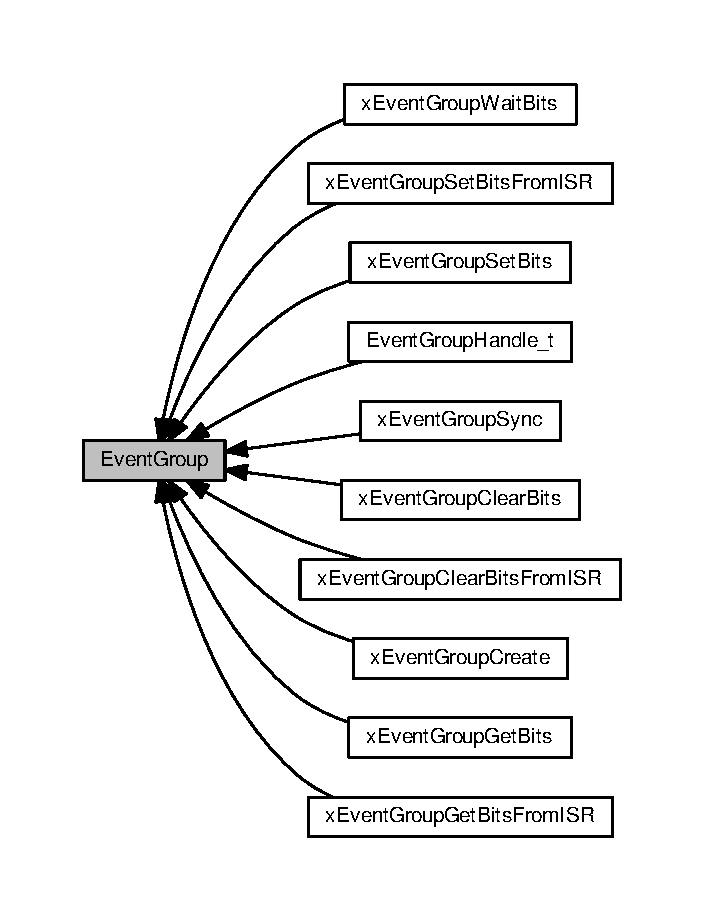
\includegraphics[width=338pt]{group___event_group}
\end{center}
\end{figure}
\subsection*{Modules}
\begin{DoxyCompactItemize}
\item 
\hyperlink{group___event_group_handle__t}{Event\+Group\+Handle\+\_\+t}
\item 
\hyperlink{group__x_event_group_create}{x\+Event\+Group\+Create}
\item 
\hyperlink{group__x_event_group_wait_bits}{x\+Event\+Group\+Wait\+Bits}
\item 
\hyperlink{group__x_event_group_clear_bits}{x\+Event\+Group\+Clear\+Bits}
\item 
\hyperlink{group__x_event_group_clear_bits_from_i_s_r}{x\+Event\+Group\+Clear\+Bits\+From\+I\+SR}
\item 
\hyperlink{group__x_event_group_set_bits}{x\+Event\+Group\+Set\+Bits}
\item 
\hyperlink{group__x_event_group_set_bits_from_i_s_r}{x\+Event\+Group\+Set\+Bits\+From\+I\+SR}
\item 
\hyperlink{group__x_event_group_sync}{x\+Event\+Group\+Sync}
\item 
\hyperlink{group__x_event_group_get_bits}{x\+Event\+Group\+Get\+Bits}
\item 
\hyperlink{group__x_event_group_get_bits_from_i_s_r}{x\+Event\+Group\+Get\+Bits\+From\+I\+SR}
\end{DoxyCompactItemize}


\subsection{Detailed Description}
An event group is a collection of bits to which an application can assign a meaning. For example, an application may create an event group to convey the status of various C\+AN bus related events in which bit 0 might mean \char`\"{}\+A C\+A\+N
message has been received and is ready for processing\char`\"{}, bit 1 might mean "The application has queued a message that is ready for sending onto the C\+AN network\char`\"{}, and bit 2 might mean \char`\"{}It is time to send a S\+Y\+NC message onto the C\+AN network" etc. A task can then test the bit values to see which events are active, and optionally enter the Blocked state to wait for a specified bit or a group of specified bits to be active. To continue the C\+AN bus example, a C\+AN controlling task can enter the Blocked state (and therefore not consume any processing time) until either bit 0, bit 1 or bit 2 are active, at which time the bit that was actually active would inform the task which action it had to take (process a received message, send a message, or send a S\+Y\+NC).

The event groups implementation contains intelligence to avoid race conditions that would otherwise occur were an application to use a simple variable for the same purpose. This is particularly important with respect to when a bit within an event group is to be cleared, and when bits have to be set and then tested atomically -\/ as is the case where event groups are used to create a synchronisation point between multiple tasks (a \textquotesingle{}rendezvous\textquotesingle{}). 
\hypertarget{group___event_group_handle__t}{}\section{Event\+Group\+Handle\+\_\+t}
\label{group___event_group_handle__t}\index{Event\+Group\+Handle\+\_\+t@{Event\+Group\+Handle\+\_\+t}}
Collaboration diagram for Event\+Group\+Handle\+\_\+t\+:\nopagebreak
\begin{figure}[H]
\begin{center}
\leavevmode
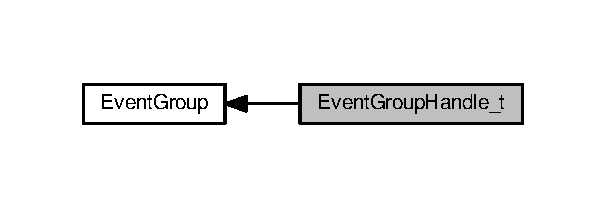
\includegraphics[width=291pt]{group___event_group_handle__t}
\end{center}
\end{figure}
\hyperlink{event__groups_8h}{event\+\_\+groups.\+h}

Type by which event groups are referenced. For example, a call to x\+Event\+Group\+Create() returns an Event\+Group\+Handle\+\_\+t variable that can then be used as a parameter to other event group functions. 
\hypertarget{group__x_event_group_create}{}\section{x\+Event\+Group\+Create}
\label{group__x_event_group_create}\index{x\+Event\+Group\+Create@{x\+Event\+Group\+Create}}
Collaboration diagram for x\+Event\+Group\+Create\+:\nopagebreak
\begin{figure}[H]
\begin{center}
\leavevmode
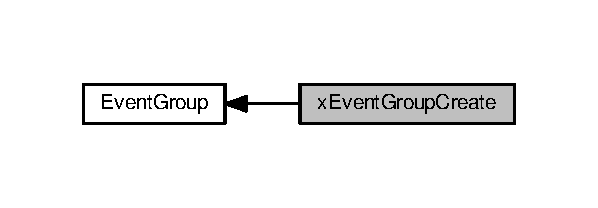
\includegraphics[width=287pt]{group__x_event_group_create}
\end{center}
\end{figure}
\hyperlink{event__groups_8h}{event\+\_\+groups.\+h} 
\begin{DoxyPre}
EventGroupHandle\_t xEventGroupCreate( void );
\end{DoxyPre}


Create a new event group.

Internally, within the Free\+R\+T\+OS implementation, event groups use a \mbox{[}small\mbox{]} block of memory, in which the event group\textquotesingle{}s structure is stored. If an event groups is created using x\+Event\+Gropu\+Create() then the required memory is automatically dynamically allocated inside the x\+Event\+Group\+Create() function. (see \href{http://www.freertos.org/a00111.html}{\tt http\+://www.\+freertos.\+org/a00111.\+html}). If an event group is created using x\+Event\+Gropu\+Create\+Static() then the application writer must instead provide the memory that will get used by the event group. x\+Event\+Group\+Create\+Static() therefore allows an event group to be created without using any dynamic memory allocation.

Although event groups are not related to ticks, for internal implementation reasons the number of bits available for use in an event group is dependent on the config\+U\+S\+E\+\_\+16\+\_\+\+B\+I\+T\+\_\+\+T\+I\+C\+KS setting in \hyperlink{_free_r_t_o_s_config_8h}{Free\+R\+T\+O\+S\+Config.\+h}. If config\+U\+S\+E\+\_\+16\+\_\+\+B\+I\+T\+\_\+\+T\+I\+C\+KS is 1 then each event group contains 8 usable bits (bit 0 to bit 7). If config\+U\+S\+E\+\_\+16\+\_\+\+B\+I\+T\+\_\+\+T\+I\+C\+KS is set to 0 then each event group has 24 usable bits (bit 0 to bit 23). The Event\+Bits\+\_\+t type is used to store event bits within an event group.

\begin{DoxyReturn}{Returns}
If the event group was created then a handle to the event group is returned. If there was insufficient Free\+R\+T\+OS heap available to create the event group then N\+U\+LL is returned. See \href{http://www.freertos.org/a00111.html}{\tt http\+://www.\+freertos.\+org/a00111.\+html}
\end{DoxyReturn}
Example usage\+: 
\begin{DoxyPre}
   // Declare a variable to hold the created event group.
   EventGroupHandle\_t xCreatedEventGroup;\end{DoxyPre}



\begin{DoxyPre}   // Attempt to create the event group.
   xCreatedEventGroup = xEventGroupCreate();\end{DoxyPre}



\begin{DoxyPre}   // Was the event group created successfully?
   if( xCreatedEventGroup == NULL )
   \{
    // The event group was not created because there was insufficient
    // FreeRTOS heap available.
   \}
   else
   \{
    // The event group was created.
   \}
  \end{DoxyPre}
 
\hypertarget{group__x_event_group_wait_bits}{}\section{x\+Event\+Group\+Wait\+Bits}
\label{group__x_event_group_wait_bits}\index{x\+Event\+Group\+Wait\+Bits@{x\+Event\+Group\+Wait\+Bits}}
Collaboration diagram for x\+Event\+Group\+Wait\+Bits\+:\nopagebreak
\begin{figure}[H]
\begin{center}
\leavevmode
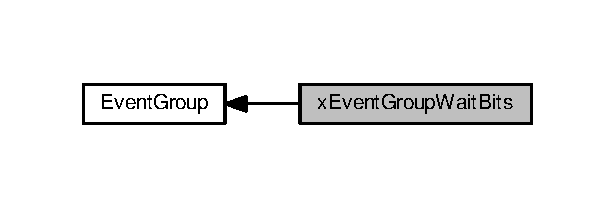
\includegraphics[width=295pt]{group__x_event_group_wait_bits}
\end{center}
\end{figure}
\hyperlink{event__groups_8h}{event\+\_\+groups.\+h} 
\begin{DoxyPre}
EventGroupHandle\_t xEventGroupCreateStatic( EventGroupHandle\_t * pxEventGroupBuffer );
\end{DoxyPre}


Create a new event group.

Internally, within the Free\+R\+T\+OS implementation, event groups use a \mbox{[}small\mbox{]} block of memory, in which the event group\textquotesingle{}s structure is stored. If an event groups is created using x\+Event\+Gropu\+Create() then the required memory is automatically dynamically allocated inside the x\+Event\+Group\+Create() function. (see \href{http://www.freertos.org/a00111.html}{\tt http\+://www.\+freertos.\+org/a00111.\+html}). If an event group is created using x\+Event\+Gropu\+Create\+Static() then the application writer must instead provide the memory that will get used by the event group. x\+Event\+Group\+Create\+Static() therefore allows an event group to be created without using any dynamic memory allocation.

Although event groups are not related to ticks, for internal implementation reasons the number of bits available for use in an event group is dependent on the config\+U\+S\+E\+\_\+16\+\_\+\+B\+I\+T\+\_\+\+T\+I\+C\+KS setting in \hyperlink{_free_r_t_o_s_config_8h}{Free\+R\+T\+O\+S\+Config.\+h}. If config\+U\+S\+E\+\_\+16\+\_\+\+B\+I\+T\+\_\+\+T\+I\+C\+KS is 1 then each event group contains 8 usable bits (bit 0 to bit 7). If config\+U\+S\+E\+\_\+16\+\_\+\+B\+I\+T\+\_\+\+T\+I\+C\+KS is set to 0 then each event group has 24 usable bits (bit 0 to bit 23). The Event\+Bits\+\_\+t type is used to store event bits within an event group.


\begin{DoxyParams}{Parameters}
{\em px\+Event\+Group\+Buffer} & px\+Event\+Group\+Buffer must point to a variable of type Static\+Event\+Group\+\_\+t, which will be then be used to hold the event group\textquotesingle{}s data structures, removing the need for the memory to be allocated dynamically.\\
\hline
\end{DoxyParams}
\begin{DoxyReturn}{Returns}
If the event group was created then a handle to the event group is returned. If px\+Event\+Group\+Buffer was N\+U\+LL then N\+U\+LL is returned.
\end{DoxyReturn}
Example usage\+: 
\begin{DoxyPre}
   // StaticEventGroup\_t is a publicly accessible structure that has the same
   // size and alignment requirements as the real event group structure.  It is
   // provided as a mechanism for applications to know the size of the event
   // group (which is dependent on the architecture and configuration file
   // settings) without breaking the strict data hiding policy by exposing the
   // real event group internals.  This StaticEventGroup\_t variable is passed
   // into the xSemaphoreCreateEventGroupStatic() function and is used to store
   // the event group's data structures
   StaticEventGroup\_t xEventGroupBuffer;\end{DoxyPre}



\begin{DoxyPre}   // Create the event group without dynamically allocating any memory.
   xEventGroup = xEventGroupCreateStatic( &xEventGroupBuffer );
  \end{DoxyPre}
 \hyperlink{event__groups_8h}{event\+\_\+groups.\+h} 
\begin{DoxyPre}
   EventBits\_t xEventGroupWaitBits(     EventGroupHandle\_t xEventGroup,
                                    const EventBits\_t uxBitsToWaitFor,
                                    const BaseType\_t xClearOnExit,
                                    const BaseType\_t xWaitForAllBits,
                                    const TickType\_t xTicksToWait );
\end{DoxyPre}


\mbox{[}Potentially\mbox{]} block to wait for one or more bits to be set within a previously created event group.

This function cannot be called from an interrupt.


\begin{DoxyParams}{Parameters}
{\em x\+Event\+Group} & The event group in which the bits are being tested. The event group must have previously been created using a call to x\+Event\+Group\+Create().\\
\hline
{\em ux\+Bits\+To\+Wait\+For} & A bitwise value that indicates the bit or bits to test inside the event group. For example, to wait for bit 0 and/or bit 2 set ux\+Bits\+To\+Wait\+For to 0x05. To wait for bits 0 and/or bit 1 and/or bit 2 set ux\+Bits\+To\+Wait\+For to 0x07. Etc.\\
\hline
{\em x\+Clear\+On\+Exit} & If x\+Clear\+On\+Exit is set to pd\+T\+R\+UE then any bits within ux\+Bits\+To\+Wait\+For that are set within the event group will be cleared before \hyperlink{event__groups_8h_aab9d5b405bc57b7624dcabe9a9a503db}{x\+Event\+Group\+Wait\+Bits()} returns if the wait condition was met (if the function returns for a reason other than a timeout). If x\+Clear\+On\+Exit is set to pd\+F\+A\+L\+SE then the bits set in the event group are not altered when the call to \hyperlink{event__groups_8h_aab9d5b405bc57b7624dcabe9a9a503db}{x\+Event\+Group\+Wait\+Bits()} returns.\\
\hline
{\em x\+Wait\+For\+All\+Bits} & If x\+Wait\+For\+All\+Bits is set to pd\+T\+R\+UE then \hyperlink{event__groups_8h_aab9d5b405bc57b7624dcabe9a9a503db}{x\+Event\+Group\+Wait\+Bits()} will return when either all the bits in ux\+Bits\+To\+Wait\+For are set or the specified block time expires. If x\+Wait\+For\+All\+Bits is set to pd\+F\+A\+L\+SE then \hyperlink{event__groups_8h_aab9d5b405bc57b7624dcabe9a9a503db}{x\+Event\+Group\+Wait\+Bits()} will return when any one of the bits set in ux\+Bits\+To\+Wait\+For is set or the specified block time expires. The block time is specified by the x\+Ticks\+To\+Wait parameter.\\
\hline
{\em x\+Ticks\+To\+Wait} & The maximum amount of time (specified in \textquotesingle{}ticks\textquotesingle{}) to wait for one/all (depending on the x\+Wait\+For\+All\+Bits value) of the bits specified by ux\+Bits\+To\+Wait\+For to become set.\\
\hline
\end{DoxyParams}
\begin{DoxyReturn}{Returns}
The value of the event group at the time either the bits being waited for became set, or the block time expired. Test the return value to know which bits were set. If \hyperlink{event__groups_8h_aab9d5b405bc57b7624dcabe9a9a503db}{x\+Event\+Group\+Wait\+Bits()} returned because its timeout expired then not all the bits being waited for will be set. If \hyperlink{event__groups_8h_aab9d5b405bc57b7624dcabe9a9a503db}{x\+Event\+Group\+Wait\+Bits()} returned because the bits it was waiting for were set then the returned value is the event group value before any bits were automatically cleared in the case that x\+Clear\+On\+Exit parameter was set to pd\+T\+R\+UE.
\end{DoxyReturn}
Example usage\+: 
\begin{DoxyPre}
  #define BIT\_0 ( 1 << 0 )
  #define BIT\_4 ( 1 << 4 )\end{DoxyPre}



\begin{DoxyPre}  void aFunction( EventGroupHandle\_t xEventGroup )
  \{
  EventBits\_t uxBits;
  const TickType\_t xTicksToWait = 100 / portTICK\_PERIOD\_MS;\end{DoxyPre}



\begin{DoxyPre}    // Wait a maximum of 100ms for either bit 0 or bit 4 to be set within
    // the event group.  Clear the bits before exiting.
    uxBits = xEventGroupWaitBits(
                xEventGroup,    // The event group being tested.
                BIT\_0 | BIT\_4,  // The bits within the event group to wait for.
                pdTRUE,         // BIT\_0 and BIT\_4 should be cleared before returning.
                pdFALSE,        // Don't wait for both bits, either bit will do.
                xTicksToWait ); // Wait a maximum of 100ms for either bit to be set.\end{DoxyPre}



\begin{DoxyPre}    if( ( uxBits \& ( BIT\_0 | BIT\_4 ) ) == ( BIT\_0 | BIT\_4 ) )
    \{
        // \hyperlink{event__groups_8h_aab9d5b405bc57b7624dcabe9a9a503db}{xEventGroupWaitBits()} returned because both bits were set.
    \}
    else if( ( uxBits \& BIT\_0 ) != 0 )
    \{
        // \hyperlink{event__groups_8h_aab9d5b405bc57b7624dcabe9a9a503db}{xEventGroupWaitBits()} returned because just BIT\_0 was set.
    \}
    else if( ( uxBits \& BIT\_4 ) != 0 )
    \{
        // \hyperlink{event__groups_8h_aab9d5b405bc57b7624dcabe9a9a503db}{xEventGroupWaitBits()} returned because just BIT\_4 was set.
    \}
    else
    \{
        // \hyperlink{event__groups_8h_aab9d5b405bc57b7624dcabe9a9a503db}{xEventGroupWaitBits()} returned because xTicksToWait ticks passed
        // without either BIT\_0 or BIT\_4 becoming set.
    \}
  \}
  \end{DoxyPre}
 
\hypertarget{group__x_event_group_clear_bits}{}\section{x\+Event\+Group\+Clear\+Bits}
\label{group__x_event_group_clear_bits}\index{x\+Event\+Group\+Clear\+Bits@{x\+Event\+Group\+Clear\+Bits}}
Collaboration diagram for x\+Event\+Group\+Clear\+Bits\+:\nopagebreak
\begin{figure}[H]
\begin{center}
\leavevmode
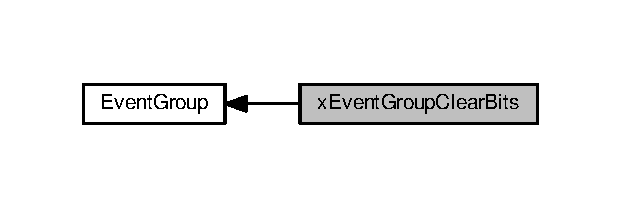
\includegraphics[width=298pt]{group__x_event_group_clear_bits}
\end{center}
\end{figure}
\hyperlink{event__groups_8h}{event\+\_\+groups.\+h} 
\begin{DoxyPre}
   EventBits\_t \hyperlink{event__groups_8h_a0fb72cfdd4f0d5f86d955fc3af448f2a}{xEventGroupClearBits( EventGroupHandle\_t xEventGroup, const EventBits\_t uxBitsToClear )};
\end{DoxyPre}


Clear bits within an event group. This function cannot be called from an interrupt.


\begin{DoxyParams}{Parameters}
{\em x\+Event\+Group} & The event group in which the bits are to be cleared.\\
\hline
{\em ux\+Bits\+To\+Clear} & A bitwise value that indicates the bit or bits to clear in the event group. For example, to clear bit 3 only, set ux\+Bits\+To\+Clear to 0x08. To clear bit 3 and bit 0 set ux\+Bits\+To\+Clear to 0x09.\\
\hline
\end{DoxyParams}
\begin{DoxyReturn}{Returns}
The value of the event group before the specified bits were cleared.
\end{DoxyReturn}
Example usage\+: 
\begin{DoxyPre}
  #define BIT\_0 ( 1 << 0 )
  #define BIT\_4 ( 1 << 4 )\end{DoxyPre}



\begin{DoxyPre}  void aFunction( EventGroupHandle\_t xEventGroup )
  \{
  EventBits\_t uxBits;\end{DoxyPre}



\begin{DoxyPre}    // Clear bit 0 and bit 4 in xEventGroup.
    uxBits = xEventGroupClearBits(
                            xEventGroup,    // The event group being updated.
                            BIT\_0 | BIT\_4 );// The bits being cleared.\end{DoxyPre}



\begin{DoxyPre}    if( ( uxBits \& ( BIT\_0 | BIT\_4 ) ) == ( BIT\_0 | BIT\_4 ) )
    \{
        // Both bit 0 and bit 4 were set before \hyperlink{event__groups_8h_a0fb72cfdd4f0d5f86d955fc3af448f2a}{xEventGroupClearBits()} was
        // called.  Both will now be clear (not set).
    \}
    else if( ( uxBits \& BIT\_0 ) != 0 )
    \{
        // Bit 0 was set before \hyperlink{event__groups_8h_a0fb72cfdd4f0d5f86d955fc3af448f2a}{xEventGroupClearBits()} was called.  It will
        // now be clear.
    \}
    else if( ( uxBits \& BIT\_4 ) != 0 )
    \{
        // Bit 4 was set before \hyperlink{event__groups_8h_a0fb72cfdd4f0d5f86d955fc3af448f2a}{xEventGroupClearBits()} was called.  It will
        // now be clear.
    \}
    else
    \{
        // Neither bit 0 nor bit 4 were set in the first place.
    \}
  \}
  \end{DoxyPre}
 
\hypertarget{group__x_event_group_clear_bits_from_i_s_r}{}\section{x\+Event\+Group\+Clear\+Bits\+From\+I\+SR}
\label{group__x_event_group_clear_bits_from_i_s_r}\index{x\+Event\+Group\+Clear\+Bits\+From\+I\+SR@{x\+Event\+Group\+Clear\+Bits\+From\+I\+SR}}
Collaboration diagram for x\+Event\+Group\+Clear\+Bits\+From\+I\+SR\+:\nopagebreak
\begin{figure}[H]
\begin{center}
\leavevmode
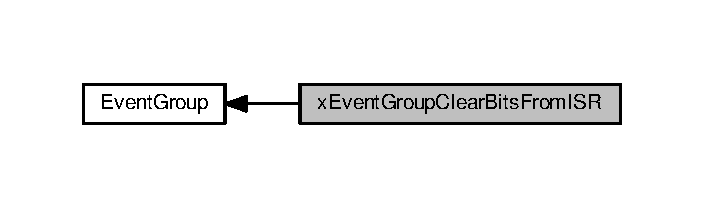
\includegraphics[width=338pt]{group__x_event_group_clear_bits_from_i_s_r}
\end{center}
\end{figure}
\hyperlink{event__groups_8h}{event\+\_\+groups.\+h} 
\begin{DoxyPre}
   BaseType\_t \hyperlink{event__groups_8h_a3d7de214a697f33fe7b914e26a93f33a}{xEventGroupClearBitsFromISR( EventGroupHandle\_t xEventGroup, const EventBits\_t uxBitsToSet )};
\end{DoxyPre}


A version of \hyperlink{event__groups_8h_a0fb72cfdd4f0d5f86d955fc3af448f2a}{x\+Event\+Group\+Clear\+Bits()} that can be called from an interrupt.

Setting bits in an event group is not a deterministic operation because there are an unknown number of tasks that may be waiting for the bit or bits being set. Free\+R\+T\+OS does not allow nondeterministic operations to be performed while interrupts are disabled, so protects event groups that are accessed from tasks by suspending the scheduler rather than disabling interrupts. As a result event groups cannot be accessed directly from an interrupt service routine. Therefore \hyperlink{event__groups_8h_a3d7de214a697f33fe7b914e26a93f33a}{x\+Event\+Group\+Clear\+Bits\+From\+I\+S\+R()} sends a message to the timer task to have the clear operation performed in the context of the timer task.


\begin{DoxyParams}{Parameters}
{\em x\+Event\+Group} & The event group in which the bits are to be cleared.\\
\hline
{\em ux\+Bits\+To\+Clear} & A bitwise value that indicates the bit or bits to clear. For example, to clear bit 3 only, set ux\+Bits\+To\+Clear to 0x08. To clear bit 3 and bit 0 set ux\+Bits\+To\+Clear to 0x09.\\
\hline
\end{DoxyParams}
\begin{DoxyReturn}{Returns}
If the request to execute the function was posted successfully then pd\+P\+A\+SS is returned, otherwise pd\+F\+A\+L\+SE is returned. pd\+F\+A\+L\+SE will be returned if the timer service queue was full.
\end{DoxyReturn}
Example usage\+: 
\begin{DoxyPre}
  #define BIT\_0 ( 1 << 0 )
  #define BIT\_4 ( 1 << 4 )\end{DoxyPre}



\begin{DoxyPre}  // An event group which it is assumed has already been created by a call to
  // xEventGroupCreate().
  EventGroupHandle\_t xEventGroup;\end{DoxyPre}



\begin{DoxyPre}  void anInterruptHandler( void )
  \{
    // Clear bit 0 and bit 4 in xEventGroup.
    xResult = xEventGroupClearBitsFromISR(
                        xEventGroup,     // The event group being updated.
                        BIT\_0 | BIT\_4 ); // The bits being set.\end{DoxyPre}



\begin{DoxyPre}    if( xResult == pdPASS )
    \{
        // The message was posted successfully.
    \}
 \}
  \end{DoxyPre}
 
\hypertarget{group__x_event_group_set_bits}{}\section{x\+Event\+Group\+Set\+Bits}
\label{group__x_event_group_set_bits}\index{x\+Event\+Group\+Set\+Bits@{x\+Event\+Group\+Set\+Bits}}
Collaboration diagram for x\+Event\+Group\+Set\+Bits\+:\nopagebreak
\begin{figure}[H]
\begin{center}
\leavevmode
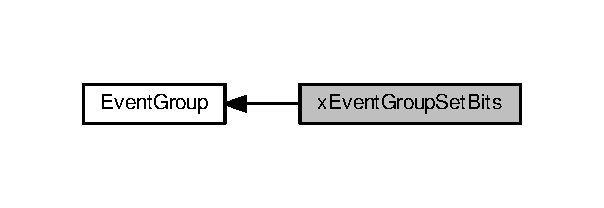
\includegraphics[width=290pt]{group__x_event_group_set_bits}
\end{center}
\end{figure}
\hyperlink{event__groups_8h}{event\+\_\+groups.\+h} 
\begin{DoxyPre}
   EventBits\_t \hyperlink{event__groups_8h_a02d7b3bb55f7e11d9c47116266c5fb2e}{xEventGroupSetBits( EventGroupHandle\_t xEventGroup, const EventBits\_t uxBitsToSet )};
\end{DoxyPre}


Set bits within an event group. This function cannot be called from an interrupt. \hyperlink{event__groups_8h_a62b68278abac6358369ae8e390988a02}{x\+Event\+Group\+Set\+Bits\+From\+I\+S\+R()} is a version that can be called from an interrupt.

Setting bits in an event group will automatically unblock tasks that are blocked waiting for the bits.


\begin{DoxyParams}{Parameters}
{\em x\+Event\+Group} & The event group in which the bits are to be set.\\
\hline
{\em ux\+Bits\+To\+Set} & A bitwise value that indicates the bit or bits to set. For example, to set bit 3 only, set ux\+Bits\+To\+Set to 0x08. To set bit 3 and bit 0 set ux\+Bits\+To\+Set to 0x09.\\
\hline
\end{DoxyParams}
\begin{DoxyReturn}{Returns}
The value of the event group at the time the call to \hyperlink{event__groups_8h_a02d7b3bb55f7e11d9c47116266c5fb2e}{x\+Event\+Group\+Set\+Bits()} returns. There are two reasons why the returned value might have the bits specified by the ux\+Bits\+To\+Set parameter cleared. First, if setting a bit results in a task that was waiting for the bit leaving the blocked state then it is possible the bit will be cleared automatically (see the x\+Clear\+Bit\+On\+Exit parameter of \hyperlink{event__groups_8h_aab9d5b405bc57b7624dcabe9a9a503db}{x\+Event\+Group\+Wait\+Bits()}). Second, any unblocked (or otherwise Ready state) task that has a priority above that of the task that called \hyperlink{event__groups_8h_a02d7b3bb55f7e11d9c47116266c5fb2e}{x\+Event\+Group\+Set\+Bits()} will execute and may change the event group value before the call to \hyperlink{event__groups_8h_a02d7b3bb55f7e11d9c47116266c5fb2e}{x\+Event\+Group\+Set\+Bits()} returns.
\end{DoxyReturn}
Example usage\+: 
\begin{DoxyPre}
  #define BIT\_0 ( 1 << 0 )
  #define BIT\_4 ( 1 << 4 )\end{DoxyPre}



\begin{DoxyPre}  void aFunction( EventGroupHandle\_t xEventGroup )
  \{
  EventBits\_t uxBits;\end{DoxyPre}



\begin{DoxyPre}    // Set bit 0 and bit 4 in xEventGroup.
    uxBits = xEventGroupSetBits(
                        xEventGroup,    // The event group being updated.
                        BIT\_0 | BIT\_4 );// The bits being set.\end{DoxyPre}



\begin{DoxyPre}    if( ( uxBits \& ( BIT\_0 | BIT\_4 ) ) == ( BIT\_0 | BIT\_4 ) )
    \{
        // Both bit 0 and bit 4 remained set when the function returned.
    \}
    else if( ( uxBits \& BIT\_0 ) != 0 )
    \{
        // Bit 0 remained set when the function returned, but bit 4 was
        // cleared.  It might be that bit 4 was cleared automatically as a
        // task that was waiting for bit 4 was removed from the Blocked
        // state.
    \}
    else if( ( uxBits \& BIT\_4 ) != 0 )
    \{
        // Bit 4 remained set when the function returned, but bit 0 was
        // cleared.  It might be that bit 0 was cleared automatically as a
        // task that was waiting for bit 0 was removed from the Blocked
        // state.
    \}
    else
    \{
        // Neither bit 0 nor bit 4 remained set.  It might be that a task
        // was waiting for both of the bits to be set, and the bits were
        // cleared as the task left the Blocked state.
    \}
  \}
  \end{DoxyPre}
 
\hypertarget{group__x_event_group_set_bits_from_i_s_r}{}\section{x\+Event\+Group\+Set\+Bits\+From\+I\+SR}
\label{group__x_event_group_set_bits_from_i_s_r}\index{x\+Event\+Group\+Set\+Bits\+From\+I\+SR@{x\+Event\+Group\+Set\+Bits\+From\+I\+SR}}
Collaboration diagram for x\+Event\+Group\+Set\+Bits\+From\+I\+SR\+:\nopagebreak
\begin{figure}[H]
\begin{center}
\leavevmode
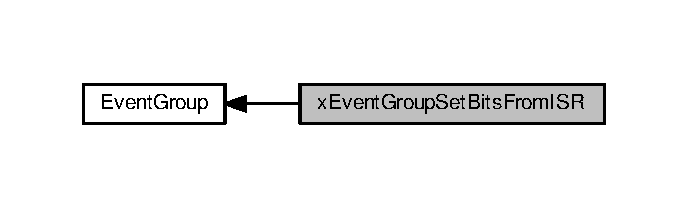
\includegraphics[width=330pt]{group__x_event_group_set_bits_from_i_s_r}
\end{center}
\end{figure}
\hyperlink{event__groups_8h}{event\+\_\+groups.\+h} 
\begin{DoxyPre}
   BaseType\_t \hyperlink{event__groups_8h_a62b68278abac6358369ae8e390988a02}{xEventGroupSetBitsFromISR( EventGroupHandle\_t xEventGroup, const EventBits\_t uxBitsToSet, BaseType\_t *pxHigherPriorityTaskWoken )};
\end{DoxyPre}


A version of \hyperlink{event__groups_8h_a02d7b3bb55f7e11d9c47116266c5fb2e}{x\+Event\+Group\+Set\+Bits()} that can be called from an interrupt.

Setting bits in an event group is not a deterministic operation because there are an unknown number of tasks that may be waiting for the bit or bits being set. Free\+R\+T\+OS does not allow nondeterministic operations to be performed in interrupts or from critical sections. Therefore \hyperlink{event__groups_8h_a62b68278abac6358369ae8e390988a02}{x\+Event\+Group\+Set\+Bits\+From\+I\+S\+R()} sends a message to the timer task to have the set operation performed in the context of the timer task -\/ where a scheduler lock is used in place of a critical section.


\begin{DoxyParams}{Parameters}
{\em x\+Event\+Group} & The event group in which the bits are to be set.\\
\hline
{\em ux\+Bits\+To\+Set} & A bitwise value that indicates the bit or bits to set. For example, to set bit 3 only, set ux\+Bits\+To\+Set to 0x08. To set bit 3 and bit 0 set ux\+Bits\+To\+Set to 0x09.\\
\hline
{\em px\+Higher\+Priority\+Task\+Woken} & As mentioned above, calling this function will result in a message being sent to the timer daemon task. If the priority of the timer daemon task is higher than the priority of the currently running task (the task the interrupt interrupted) then $\ast$px\+Higher\+Priority\+Task\+Woken will be set to pd\+T\+R\+UE by \hyperlink{event__groups_8h_a62b68278abac6358369ae8e390988a02}{x\+Event\+Group\+Set\+Bits\+From\+I\+S\+R()}, indicating that a context switch should be requested before the interrupt exits. For that reason $\ast$px\+Higher\+Priority\+Task\+Woken must be initialised to pd\+F\+A\+L\+SE. See the example code below.\\
\hline
\end{DoxyParams}
\begin{DoxyReturn}{Returns}
If the request to execute the function was posted successfully then pd\+P\+A\+SS is returned, otherwise pd\+F\+A\+L\+SE is returned. pd\+F\+A\+L\+SE will be returned if the timer service queue was full.
\end{DoxyReturn}
Example usage\+: 
\begin{DoxyPre}
  #define BIT\_0 ( 1 << 0 )
  #define BIT\_4 ( 1 << 4 )\end{DoxyPre}



\begin{DoxyPre}  // An event group which it is assumed has already been created by a call to
  // xEventGroupCreate().
  EventGroupHandle\_t xEventGroup;\end{DoxyPre}



\begin{DoxyPre}  void anInterruptHandler( void )
  \{
  BaseType\_t xHigherPriorityTaskWoken, xResult;\end{DoxyPre}



\begin{DoxyPre}    // xHigherPriorityTaskWoken must be initialised to pdFALSE.
    xHigherPriorityTaskWoken = pdFALSE;\end{DoxyPre}



\begin{DoxyPre}    // Set bit 0 and bit 4 in xEventGroup.
    xResult = xEventGroupSetBitsFromISR(
                        xEventGroup,    // The event group being updated.
                        BIT\_0 | BIT\_4   // The bits being set.
                        \&xHigherPriorityTaskWoken );\end{DoxyPre}



\begin{DoxyPre}    // Was the message posted successfully?
    if( xResult == pdPASS )
    \{
        // If xHigherPriorityTaskWoken is now set to pdTRUE then a context
        // switch should be requested.  The macro used is port specific and
        // will be either \hyperlink{portmacro_8h_aac6850c66595efdc02a8bbb95fb4648e}{portYIELD\_FROM\_ISR()} or \hyperlink{portmacro_8h_a63b994040c62c9685490a71c87a13d8a}{portEND\_SWITCHING\_ISR()} -
        // refer to the documentation page for the port being used.
        \hyperlink{portmacro_8h_aac6850c66595efdc02a8bbb95fb4648e}{portYIELD\_FROM\_ISR( xHigherPriorityTaskWoken )};
    \}
 \}
  \end{DoxyPre}
 
\hypertarget{group__x_event_group_sync}{}\section{x\+Event\+Group\+Sync}
\label{group__x_event_group_sync}\index{x\+Event\+Group\+Sync@{x\+Event\+Group\+Sync}}
Collaboration diagram for x\+Event\+Group\+Sync\+:\nopagebreak
\begin{figure}[H]
\begin{center}
\leavevmode
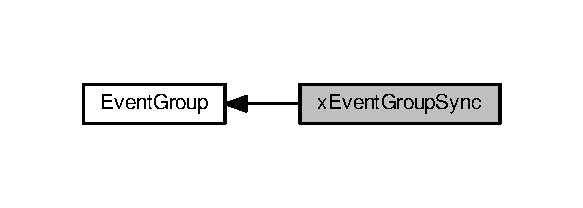
\includegraphics[width=280pt]{group__x_event_group_sync}
\end{center}
\end{figure}
\hyperlink{event__groups_8h}{event\+\_\+groups.\+h} 
\begin{DoxyPre}
   EventBits\_t xEventGroupSync( EventGroupHandle\_t xEventGroup,
                                const EventBits\_t uxBitsToSet,
                                const EventBits\_t uxBitsToWaitFor,
                                TickType\_t xTicksToWait );
\end{DoxyPre}


Atomically set bits within an event group, then wait for a combination of bits to be set within the same event group. This functionality is typically used to synchronise multiple tasks, where each task has to wait for the other tasks to reach a synchronisation point before proceeding.

This function cannot be used from an interrupt.

The function will return before its block time expires if the bits specified by the ux\+Bits\+To\+Wait parameter are set, or become set within that time. In this case all the bits specified by ux\+Bits\+To\+Wait will be automatically cleared before the function returns.


\begin{DoxyParams}{Parameters}
{\em x\+Event\+Group} & The event group in which the bits are being tested. The event group must have previously been created using a call to x\+Event\+Group\+Create().\\
\hline
{\em ux\+Bits\+To\+Set} & The bits to set in the event group before determining if, and possibly waiting for, all the bits specified by the ux\+Bits\+To\+Wait parameter are set.\\
\hline
{\em ux\+Bits\+To\+Wait\+For} & A bitwise value that indicates the bit or bits to test inside the event group. For example, to wait for bit 0 and bit 2 set ux\+Bits\+To\+Wait\+For to 0x05. To wait for bits 0 and bit 1 and bit 2 set ux\+Bits\+To\+Wait\+For to 0x07. Etc.\\
\hline
{\em x\+Ticks\+To\+Wait} & The maximum amount of time (specified in \textquotesingle{}ticks\textquotesingle{}) to wait for all of the bits specified by ux\+Bits\+To\+Wait\+For to become set.\\
\hline
\end{DoxyParams}
\begin{DoxyReturn}{Returns}
The value of the event group at the time either the bits being waited for became set, or the block time expired. Test the return value to know which bits were set. If \hyperlink{event__groups_8h_a869511456b86426f52e2eec898bff341}{x\+Event\+Group\+Sync()} returned because its timeout expired then not all the bits being waited for will be set. If \hyperlink{event__groups_8h_a869511456b86426f52e2eec898bff341}{x\+Event\+Group\+Sync()} returned because all the bits it was waiting for were set then the returned value is the event group value before any bits were automatically cleared.
\end{DoxyReturn}
Example usage\+: 
\begin{DoxyPre}
// Bits used by the three tasks.
#define TASK\_0\_BIT      ( 1 << 0 )
#define TASK\_1\_BIT      ( 1 << 1 )
#define TASK\_2\_BIT      ( 1 << 2 )\end{DoxyPre}



\begin{DoxyPre}#define ALL\_SYNC\_BITS ( TASK\_0\_BIT | TASK\_1\_BIT | TASK\_2\_BIT )\end{DoxyPre}



\begin{DoxyPre}// Use an event group to synchronise three tasks.  It is assumed this event
// group has already been created elsewhere.
EventGroupHandle\_t xEventBits;\end{DoxyPre}



\begin{DoxyPre}void vTask0( void *pvParameters )
\{
EventBits\_t uxReturn;
TickType\_t xTicksToWait = 100 / portTICK\_PERIOD\_MS;
\begin{DoxyVerb}for( ;; )
{
// Perform task functionality here.

// Set bit 0 in the event flag to note this task has reached the
// sync point.  The other two tasks will set the other two bits defined
// by ALL_SYNC_BITS.  All three tasks have reached the synchronisation
// point when all the ALL_SYNC_BITS are set.  Wait a maximum of 100ms
// for this to happen.
uxReturn = xEventGroupSync( xEventBits, TASK_0_BIT, ALL_SYNC_BITS, xTicksToWait );

if( ( uxReturn & ALL_SYNC_BITS ) == ALL_SYNC_BITS )
{
    // All three tasks reached the synchronisation point before the call
    // to xEventGroupSync() timed out.
}
\end{DoxyVerb}

   \}
\}\end{DoxyPre}



\begin{DoxyPre}void vTask1( void *pvParameters )
\{
    for( ;; )
    \{
    // Perform task functionality here.\end{DoxyPre}



\begin{DoxyPre}    // Set bit 1 in the event flag to note this task has reached the
    // synchronisation point.  The other two tasks will set the other two
    // bits defined by ALL\_SYNC\_BITS.  All three tasks have reached the
    // synchronisation point when all the ALL\_SYNC\_BITS are set.  Wait
    // indefinitely for this to happen.
    xEventGroupSync( xEventBits, TASK\_1\_BIT, ALL\_SYNC\_BITS, portMAX\_DELAY );\end{DoxyPre}



\begin{DoxyPre}    // \hyperlink{event__groups_8h_a869511456b86426f52e2eec898bff341}{xEventGroupSync()} was called with an indefinite block time, so
    // this task will only reach here if the syncrhonisation was made by all
    // three tasks, so there is no need to test the return value.
    \}
\}\end{DoxyPre}



\begin{DoxyPre}void vTask2( void *pvParameters )
\{
    for( ;; )
    \{
    // Perform task functionality here.\end{DoxyPre}



\begin{DoxyPre}    // Set bit 2 in the event flag to note this task has reached the
    // synchronisation point.  The other two tasks will set the other two
    // bits defined by ALL\_SYNC\_BITS.  All three tasks have reached the
    // synchronisation point when all the ALL\_SYNC\_BITS are set.  Wait
    // indefinitely for this to happen.
    xEventGroupSync( xEventBits, TASK\_2\_BIT, ALL\_SYNC\_BITS, portMAX\_DELAY );\end{DoxyPre}



\begin{DoxyPre}    // \hyperlink{event__groups_8h_a869511456b86426f52e2eec898bff341}{xEventGroupSync()} was called with an indefinite block time, so
    // this task will only reach here if the syncrhonisation was made by all
    // three tasks, so there is no need to test the return value.
   \}
\}\end{DoxyPre}



\begin{DoxyPre}\end{DoxyPre}
 
\hypertarget{group__x_event_group_get_bits}{}\section{x\+Event\+Group\+Get\+Bits}
\label{group__x_event_group_get_bits}\index{x\+Event\+Group\+Get\+Bits@{x\+Event\+Group\+Get\+Bits}}
Collaboration diagram for x\+Event\+Group\+Get\+Bits\+:\nopagebreak
\begin{figure}[H]
\begin{center}
\leavevmode
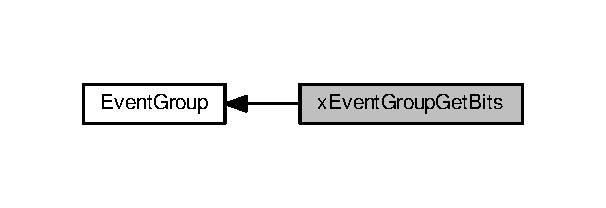
\includegraphics[width=291pt]{group__x_event_group_get_bits}
\end{center}
\end{figure}
\hyperlink{event__groups_8h}{event\+\_\+groups.\+h} 
\begin{DoxyPre}
   EventBits\_t \hyperlink{event__groups_8h_a0ae86f092fb07ccb475ae938f9a12584}{xEventGroupGetBits( EventGroupHandle\_t xEventGroup )};
\end{DoxyPre}


Returns the current value of the bits in an event group. This function cannot be used from an interrupt.


\begin{DoxyParams}{Parameters}
{\em x\+Event\+Group} & The event group being queried.\\
\hline
\end{DoxyParams}
\begin{DoxyReturn}{Returns}
The event group bits at the time \hyperlink{event__groups_8h_a0ae86f092fb07ccb475ae938f9a12584}{x\+Event\+Group\+Get\+Bits()} was called. 
\end{DoxyReturn}

\hypertarget{group__x_event_group_get_bits_from_i_s_r}{}\section{x\+Event\+Group\+Get\+Bits\+From\+I\+SR}
\label{group__x_event_group_get_bits_from_i_s_r}\index{x\+Event\+Group\+Get\+Bits\+From\+I\+SR@{x\+Event\+Group\+Get\+Bits\+From\+I\+SR}}
Collaboration diagram for x\+Event\+Group\+Get\+Bits\+From\+I\+SR\+:\nopagebreak
\begin{figure}[H]
\begin{center}
\leavevmode
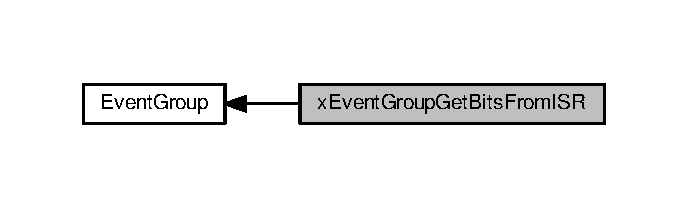
\includegraphics[width=330pt]{group__x_event_group_get_bits_from_i_s_r}
\end{center}
\end{figure}
\hyperlink{event__groups_8h}{event\+\_\+groups.\+h} 
\begin{DoxyPre}
   EventBits\_t \hyperlink{event__groups_8h_a95822db4357d0b77c35aed0c7427eca0}{xEventGroupGetBitsFromISR( EventGroupHandle\_t xEventGroup )};
\end{DoxyPre}


A version of \hyperlink{event__groups_8h_a0ae86f092fb07ccb475ae938f9a12584}{x\+Event\+Group\+Get\+Bits()} that can be called from an I\+SR.


\begin{DoxyParams}{Parameters}
{\em x\+Event\+Group} & The event group being queried.\\
\hline
\end{DoxyParams}
\begin{DoxyReturn}{Returns}
The event group bits at the time \hyperlink{event__groups_8h_a95822db4357d0b77c35aed0c7427eca0}{x\+Event\+Group\+Get\+Bits\+From\+I\+S\+R()} was called. 
\end{DoxyReturn}

\hypertarget{group__x_queue_create}{}\section{x\+Queue\+Create}
\label{group__x_queue_create}\index{x\+Queue\+Create@{x\+Queue\+Create}}
queue. h 
\begin{DoxyPre}
QueueHandle\_t xQueueCreate(
                          UBaseType\_t uxQueueLength,
                          UBaseType\_t uxItemSize
                      );
  \end{DoxyPre}


Creates a new queue instance, and returns a handle by which the new queue can be referenced.

Internally, within the Free\+R\+T\+OS implementation, queues use two blocks of memory. The first block is used to hold the queue\textquotesingle{}s data structures. The second block is used to hold items placed into the queue. If a queue is created using x\+Queue\+Create() then both blocks of memory are automatically dynamically allocated inside the x\+Queue\+Create() function. (see \href{http://www.freertos.org/a00111.html}{\tt http\+://www.\+freertos.\+org/a00111.\+html}). If a queue is created using x\+Queue\+Create\+Static() then the application writer must provide the memory that will get used by the queue. x\+Queue\+Create\+Static() therefore allows a queue to be created without using any dynamic memory allocation.

\href{http://www.FreeRTOS.org/Embedded-RTOS-Queues.html}{\tt http\+://www.\+Free\+R\+T\+O\+S.\+org/\+Embedded-\/\+R\+T\+O\+S-\/\+Queues.\+html}


\begin{DoxyParams}{Parameters}
{\em ux\+Queue\+Length} & The maximum number of items that the queue can contain.\\
\hline
{\em ux\+Item\+Size} & The number of bytes each item in the queue will require. Items are queued by copy, not by reference, so this is the number of bytes that will be copied for each posted item. Each item on the queue must be the same size.\\
\hline
\end{DoxyParams}
\begin{DoxyReturn}{Returns}
If the queue is successfully create then a handle to the newly created queue is returned. If the queue cannot be created then 0 is returned.
\end{DoxyReturn}
Example usage\+: 
\begin{DoxyPre}
struct AMessage
\{
   char ucMessageID;
   char ucData[ 20 ];
\};\end{DoxyPre}



\begin{DoxyPre}void vATask( void *pvParameters )
\{
QueueHandle\_t xQueue1, xQueue2;\end{DoxyPre}



\begin{DoxyPre}   // Create a queue capable of containing 10 uint32\_t values.
   xQueue1 = xQueueCreate( 10, sizeof( uint32\_t ) );
   if( xQueue1 == 0 )
   \{
    // Queue was not created and must not be used.
   \}\end{DoxyPre}



\begin{DoxyPre}   // Create a queue capable of containing 10 pointers to AMessage structures.
   // These should be passed by pointer as they contain a lot of data.
   xQueue2 = xQueueCreate( 10, sizeof( struct AMessage * ) );
   if( xQueue2 == 0 )
   \{
    // Queue was not created and must not be used.
   \}\end{DoxyPre}



\begin{DoxyPre}   // ... Rest of task code.
\}
\end{DoxyPre}
 
\hypertarget{group__x_queue_create_static}{}\section{x\+Queue\+Create\+Static}
\label{group__x_queue_create_static}\index{x\+Queue\+Create\+Static@{x\+Queue\+Create\+Static}}
queue. h 
\begin{DoxyPre}
QueueHandle\_t xQueueCreateStatic(
                          UBaseType\_t uxQueueLength,
                          UBaseType\_t uxItemSize,
                          uint8\_t *pucQueueStorageBuffer,
                          StaticQueue\_t *pxQueueBuffer
                      );
  \end{DoxyPre}


Creates a new queue instance, and returns a handle by which the new queue can be referenced.

Internally, within the Free\+R\+T\+OS implementation, queues use two blocks of memory. The first block is used to hold the queue\textquotesingle{}s data structures. The second block is used to hold items placed into the queue. If a queue is created using x\+Queue\+Create() then both blocks of memory are automatically dynamically allocated inside the x\+Queue\+Create() function. (see \href{http://www.freertos.org/a00111.html}{\tt http\+://www.\+freertos.\+org/a00111.\+html}). If a queue is created using x\+Queue\+Create\+Static() then the application writer must provide the memory that will get used by the queue. x\+Queue\+Create\+Static() therefore allows a queue to be created without using any dynamic memory allocation.

\href{http://www.FreeRTOS.org/Embedded-RTOS-Queues.html}{\tt http\+://www.\+Free\+R\+T\+O\+S.\+org/\+Embedded-\/\+R\+T\+O\+S-\/\+Queues.\+html}


\begin{DoxyParams}{Parameters}
{\em ux\+Queue\+Length} & The maximum number of items that the queue can contain.\\
\hline
{\em ux\+Item\+Size} & The number of bytes each item in the queue will require. Items are queued by copy, not by reference, so this is the number of bytes that will be copied for each posted item. Each item on the queue must be the same size.\\
\hline
{\em puc\+Queue\+Storage\+Buffer} & If ux\+Item\+Size is not zero then puc\+Queue\+Storage\+Buffer must point to a uint8\+\_\+t array that is at least large enough to hold the maximum number of items that can be in the queue at any one time -\/ which is ( ux\+Queue\+Length $\ast$ ux\+Items\+Size ) bytes. If ux\+Item\+Size is zero then puc\+Queue\+Storage\+Buffer can be N\+U\+LL.\\
\hline
{\em px\+Queue\+Buffer} & Must point to a variable of type Static\+Queue\+\_\+t, which will be used to hold the queue\textquotesingle{}s data structure.\\
\hline
\end{DoxyParams}
\begin{DoxyReturn}{Returns}
If the queue is created then a handle to the created queue is returned. If px\+Queue\+Buffer is N\+U\+LL then N\+U\+LL is returned.
\end{DoxyReturn}
Example usage\+: 
\begin{DoxyPre}
struct AMessage
\{
   char ucMessageID;
   char ucData[ 20 ];
\};\end{DoxyPre}



\begin{DoxyPre}#define QUEUE\_LENGTH 10
#define ITEM\_SIZE sizeof( uint32\_t )\end{DoxyPre}



\begin{DoxyPre}// xQueueBuffer will hold the queue structure.
StaticQueue\_t xQueueBuffer;\end{DoxyPre}



\begin{DoxyPre}// ucQueueStorage will hold the items posted to the queue.  Must be at least
// [(queue length) * ( queue item size)] bytes long.
uint8\_t ucQueueStorage[ QUEUE\_LENGTH * ITEM\_SIZE ];\end{DoxyPre}



\begin{DoxyPre}void vATask( void *pvParameters )
\{
QueueHandle\_t xQueue1;\end{DoxyPre}



\begin{DoxyPre}   // Create a queue capable of containing 10 uint32\_t values.
   xQueue1 = xQueueCreate( QUEUE\_LENGTH, // The number of items the queue can hold.
                        ITEM\_SIZE     // The size of each item in the queue
                        \&( ucQueueStorage[ 0 ] ), // The buffer that will hold the items in the queue.
                        \&xQueueBuffer ); // The buffer that will hold the queue structure.\end{DoxyPre}



\begin{DoxyPre}   // The queue is guaranteed to be created successfully as no dynamic memory
   // allocation is used.  Therefore xQueue1 is now a handle to a valid queue.\end{DoxyPre}



\begin{DoxyPre}   // ... Rest of task code.
\}
\end{DoxyPre}
 
\hypertarget{group__x_queue_send}{}\section{x\+Queue\+Send}
\label{group__x_queue_send}\index{x\+Queue\+Send@{x\+Queue\+Send}}
queue. h 
\begin{DoxyPre}
BaseType\_t xQueueSendToToFront(
                               QueueHandle\_t    xQueue,
                               const void       *pvItemToQueue,
                               TickType\_t       xTicksToWait
                           );
  \end{DoxyPre}


This is a macro that calls \hyperlink{queue_8h_a7ce86d1026e0c3055a523935bf53c0b3}{x\+Queue\+Generic\+Send()}.

Post an item to the front of a queue. The item is queued by copy, not by reference. This function must not be called from an interrupt service routine. See x\+Queue\+Send\+From\+I\+SR () for an alternative which may be used in an I\+SR.


\begin{DoxyParams}{Parameters}
{\em x\+Queue} & The handle to the queue on which the item is to be posted.\\
\hline
{\em pv\+Item\+To\+Queue} & A pointer to the item that is to be placed on the queue. The size of the items the queue will hold was defined when the queue was created, so this many bytes will be copied from pv\+Item\+To\+Queue into the queue storage area.\\
\hline
{\em x\+Ticks\+To\+Wait} & The maximum amount of time the task should block waiting for space to become available on the queue, should it already be full. The call will return immediately if this is set to 0 and the queue is full. The time is defined in tick periods so the constant port\+T\+I\+C\+K\+\_\+\+P\+E\+R\+I\+O\+D\+\_\+\+MS should be used to convert to real time if this is required.\\
\hline
\end{DoxyParams}
\begin{DoxyReturn}{Returns}
pd\+T\+R\+UE if the item was successfully posted, otherwise err\+Q\+U\+E\+U\+E\+\_\+\+F\+U\+LL.
\end{DoxyReturn}
Example usage\+: 
\begin{DoxyPre}
struct AMessage
\{
   char ucMessageID;
   char ucData[ 20 ];
\} xMessage;\end{DoxyPre}



\begin{DoxyPre}uint32\_t ulVar = 10UL;\end{DoxyPre}



\begin{DoxyPre}void vATask( void *pvParameters )
\{
QueueHandle\_t xQueue1, xQueue2;
struct AMessage *pxMessage;\end{DoxyPre}



\begin{DoxyPre}   // Create a queue capable of containing 10 uint32\_t values.
   xQueue1 = xQueueCreate( 10, sizeof( uint32\_t ) );\end{DoxyPre}



\begin{DoxyPre}   // Create a queue capable of containing 10 pointers to AMessage structures.
   // These should be passed by pointer as they contain a lot of data.
   xQueue2 = xQueueCreate( 10, sizeof( struct AMessage * ) );\end{DoxyPre}



\begin{DoxyPre}   // ...\end{DoxyPre}



\begin{DoxyPre}   if( xQueue1 != 0 )
   \{
    // Send an uint32\_t.  Wait for 10 ticks for space to become
    // available if necessary.
    if( xQueueSendToFront( xQueue1, ( void * ) \&ulVar, ( TickType\_t ) 10 ) != pdPASS )
    \{
        // Failed to post the message, even after 10 ticks.
    \}
   \}\end{DoxyPre}



\begin{DoxyPre}   if( xQueue2 != 0 )
   \{
    // Send a pointer to a struct AMessage object.  Don't block if the
    // queue is already full.
    pxMessage = \& xMessage;
    xQueueSendToFront( xQueue2, ( void * ) \&pxMessage, ( TickType\_t ) 0 );
   \}\end{DoxyPre}



\begin{DoxyPre}   // ... Rest of task code.
\}
\end{DoxyPre}


queue. h 
\begin{DoxyPre}
BaseType\_t xQueueSendToBack(
                               QueueHandle\_t    xQueue,
                               const void       *pvItemToQueue,
                               TickType\_t       xTicksToWait
                           );
  \end{DoxyPre}


This is a macro that calls \hyperlink{queue_8h_a7ce86d1026e0c3055a523935bf53c0b3}{x\+Queue\+Generic\+Send()}.

Post an item to the back of a queue. The item is queued by copy, not by reference. This function must not be called from an interrupt service routine. See x\+Queue\+Send\+From\+I\+SR () for an alternative which may be used in an I\+SR.


\begin{DoxyParams}{Parameters}
{\em x\+Queue} & The handle to the queue on which the item is to be posted.\\
\hline
{\em pv\+Item\+To\+Queue} & A pointer to the item that is to be placed on the queue. The size of the items the queue will hold was defined when the queue was created, so this many bytes will be copied from pv\+Item\+To\+Queue into the queue storage area.\\
\hline
{\em x\+Ticks\+To\+Wait} & The maximum amount of time the task should block waiting for space to become available on the queue, should it already be full. The call will return immediately if this is set to 0 and the queue is full. The time is defined in tick periods so the constant port\+T\+I\+C\+K\+\_\+\+P\+E\+R\+I\+O\+D\+\_\+\+MS should be used to convert to real time if this is required.\\
\hline
\end{DoxyParams}
\begin{DoxyReturn}{Returns}
pd\+T\+R\+UE if the item was successfully posted, otherwise err\+Q\+U\+E\+U\+E\+\_\+\+F\+U\+LL.
\end{DoxyReturn}
Example usage\+: 
\begin{DoxyPre}
struct AMessage
\{
   char ucMessageID;
   char ucData[ 20 ];
\} xMessage;\end{DoxyPre}



\begin{DoxyPre}uint32\_t ulVar = 10UL;\end{DoxyPre}



\begin{DoxyPre}void vATask( void *pvParameters )
\{
QueueHandle\_t xQueue1, xQueue2;
struct AMessage *pxMessage;\end{DoxyPre}



\begin{DoxyPre}   // Create a queue capable of containing 10 uint32\_t values.
   xQueue1 = xQueueCreate( 10, sizeof( uint32\_t ) );\end{DoxyPre}



\begin{DoxyPre}   // Create a queue capable of containing 10 pointers to AMessage structures.
   // These should be passed by pointer as they contain a lot of data.
   xQueue2 = xQueueCreate( 10, sizeof( struct AMessage * ) );\end{DoxyPre}



\begin{DoxyPre}   // ...\end{DoxyPre}



\begin{DoxyPre}   if( xQueue1 != 0 )
   \{
    // Send an uint32\_t.  Wait for 10 ticks for space to become
    // available if necessary.
    if( xQueueSendToBack( xQueue1, ( void * ) \&ulVar, ( TickType\_t ) 10 ) != pdPASS )
    \{
        // Failed to post the message, even after 10 ticks.
    \}
   \}\end{DoxyPre}



\begin{DoxyPre}   if( xQueue2 != 0 )
   \{
    // Send a pointer to a struct AMessage object.  Don't block if the
    // queue is already full.
    pxMessage = \& xMessage;
    xQueueSendToBack( xQueue2, ( void * ) \&pxMessage, ( TickType\_t ) 0 );
   \}\end{DoxyPre}



\begin{DoxyPre}   // ... Rest of task code.
\}
\end{DoxyPre}


queue. h 
\begin{DoxyPre}
BaseType\_t xQueueSend(
                          QueueHandle\_t xQueue,
                          const void * pvItemToQueue,
                          TickType\_t xTicksToWait
                     );
  \end{DoxyPre}


This is a macro that calls \hyperlink{queue_8h_a7ce86d1026e0c3055a523935bf53c0b3}{x\+Queue\+Generic\+Send()}. It is included for backward compatibility with versions of Free\+R\+T\+O\+S.\+org that did not include the \hyperlink{queue_8h_aa612fcc2b1ceee0200f34b942e300b41}{x\+Queue\+Send\+To\+Front()} and \hyperlink{queue_8h_a81d24a2c1199d58efb76fbee15853112}{x\+Queue\+Send\+To\+Back()} macros. It is equivalent to \hyperlink{queue_8h_a81d24a2c1199d58efb76fbee15853112}{x\+Queue\+Send\+To\+Back()}.

Post an item on a queue. The item is queued by copy, not by reference. This function must not be called from an interrupt service routine. See x\+Queue\+Send\+From\+I\+SR () for an alternative which may be used in an I\+SR.


\begin{DoxyParams}{Parameters}
{\em x\+Queue} & The handle to the queue on which the item is to be posted.\\
\hline
{\em pv\+Item\+To\+Queue} & A pointer to the item that is to be placed on the queue. The size of the items the queue will hold was defined when the queue was created, so this many bytes will be copied from pv\+Item\+To\+Queue into the queue storage area.\\
\hline
{\em x\+Ticks\+To\+Wait} & The maximum amount of time the task should block waiting for space to become available on the queue, should it already be full. The call will return immediately if this is set to 0 and the queue is full. The time is defined in tick periods so the constant port\+T\+I\+C\+K\+\_\+\+P\+E\+R\+I\+O\+D\+\_\+\+MS should be used to convert to real time if this is required.\\
\hline
\end{DoxyParams}
\begin{DoxyReturn}{Returns}
pd\+T\+R\+UE if the item was successfully posted, otherwise err\+Q\+U\+E\+U\+E\+\_\+\+F\+U\+LL.
\end{DoxyReturn}
Example usage\+: 
\begin{DoxyPre}
struct AMessage
\{
   char ucMessageID;
   char ucData[ 20 ];
\} xMessage;\end{DoxyPre}



\begin{DoxyPre}uint32\_t ulVar = 10UL;\end{DoxyPre}



\begin{DoxyPre}void vATask( void *pvParameters )
\{
QueueHandle\_t xQueue1, xQueue2;
struct AMessage *pxMessage;\end{DoxyPre}



\begin{DoxyPre}   // Create a queue capable of containing 10 uint32\_t values.
   xQueue1 = xQueueCreate( 10, sizeof( uint32\_t ) );\end{DoxyPre}



\begin{DoxyPre}   // Create a queue capable of containing 10 pointers to AMessage structures.
   // These should be passed by pointer as they contain a lot of data.
   xQueue2 = xQueueCreate( 10, sizeof( struct AMessage * ) );\end{DoxyPre}



\begin{DoxyPre}   // ...\end{DoxyPre}



\begin{DoxyPre}   if( xQueue1 != 0 )
   \{
    // Send an uint32\_t.  Wait for 10 ticks for space to become
    // available if necessary.
    if( xQueueSend( xQueue1, ( void * ) \&ulVar, ( TickType\_t ) 10 ) != pdPASS )
    \{
        // Failed to post the message, even after 10 ticks.
    \}
   \}\end{DoxyPre}



\begin{DoxyPre}   if( xQueue2 != 0 )
   \{
    // Send a pointer to a struct AMessage object.  Don't block if the
    // queue is already full.
    pxMessage = \& xMessage;
    xQueueSend( xQueue2, ( void * ) \&pxMessage, ( TickType\_t ) 0 );
   \}\end{DoxyPre}



\begin{DoxyPre}   // ... Rest of task code.
\}
\end{DoxyPre}


queue. h 
\begin{DoxyPre}
BaseType\_t xQueueGenericSend(
                                QueueHandle\_t xQueue,
                                const void * pvItemToQueue,
                                TickType\_t xTicksToWait
                                BaseType\_t xCopyPosition
                            );
  \end{DoxyPre}


It is preferred that the macros \hyperlink{queue_8h_af7eb49d3249351176992950d9185abe9}{x\+Queue\+Send()}, \hyperlink{queue_8h_aa612fcc2b1ceee0200f34b942e300b41}{x\+Queue\+Send\+To\+Front()} and \hyperlink{queue_8h_a81d24a2c1199d58efb76fbee15853112}{x\+Queue\+Send\+To\+Back()} are used in place of calling this function directly.

Post an item on a queue. The item is queued by copy, not by reference. This function must not be called from an interrupt service routine. See x\+Queue\+Send\+From\+I\+SR () for an alternative which may be used in an I\+SR.


\begin{DoxyParams}{Parameters}
{\em x\+Queue} & The handle to the queue on which the item is to be posted.\\
\hline
{\em pv\+Item\+To\+Queue} & A pointer to the item that is to be placed on the queue. The size of the items the queue will hold was defined when the queue was created, so this many bytes will be copied from pv\+Item\+To\+Queue into the queue storage area.\\
\hline
{\em x\+Ticks\+To\+Wait} & The maximum amount of time the task should block waiting for space to become available on the queue, should it already be full. The call will return immediately if this is set to 0 and the queue is full. The time is defined in tick periods so the constant port\+T\+I\+C\+K\+\_\+\+P\+E\+R\+I\+O\+D\+\_\+\+MS should be used to convert to real time if this is required.\\
\hline
{\em x\+Copy\+Position} & Can take the value queue\+S\+E\+N\+D\+\_\+\+T\+O\+\_\+\+B\+A\+CK to place the item at the back of the queue, or queue\+S\+E\+N\+D\+\_\+\+T\+O\+\_\+\+F\+R\+O\+NT to place the item at the front of the queue (for high priority messages).\\
\hline
\end{DoxyParams}
\begin{DoxyReturn}{Returns}
pd\+T\+R\+UE if the item was successfully posted, otherwise err\+Q\+U\+E\+U\+E\+\_\+\+F\+U\+LL.
\end{DoxyReturn}
Example usage\+: 
\begin{DoxyPre}
struct AMessage
\{
   char ucMessageID;
   char ucData[ 20 ];
\} xMessage;\end{DoxyPre}



\begin{DoxyPre}uint32\_t ulVar = 10UL;\end{DoxyPre}



\begin{DoxyPre}void vATask( void *pvParameters )
\{
QueueHandle\_t xQueue1, xQueue2;
struct AMessage *pxMessage;\end{DoxyPre}



\begin{DoxyPre}   // Create a queue capable of containing 10 uint32\_t values.
   xQueue1 = xQueueCreate( 10, sizeof( uint32\_t ) );\end{DoxyPre}



\begin{DoxyPre}   // Create a queue capable of containing 10 pointers to AMessage structures.
   // These should be passed by pointer as they contain a lot of data.
   xQueue2 = xQueueCreate( 10, sizeof( struct AMessage * ) );\end{DoxyPre}



\begin{DoxyPre}   // ...\end{DoxyPre}



\begin{DoxyPre}   if( xQueue1 != 0 )
   \{
    // Send an uint32\_t.  Wait for 10 ticks for space to become
    // available if necessary.
    if( xQueueGenericSend( xQueue1, ( void * ) \&ulVar, ( TickType\_t ) 10, queueSEND\_TO\_BACK ) != pdPASS )
    \{
        // Failed to post the message, even after 10 ticks.
    \}
   \}\end{DoxyPre}



\begin{DoxyPre}   if( xQueue2 != 0 )
   \{
    // Send a pointer to a struct AMessage object.  Don't block if the
    // queue is already full.
    pxMessage = \& xMessage;
    xQueueGenericSend( xQueue2, ( void * ) \&pxMessage, ( TickType\_t ) 0, queueSEND\_TO\_BACK );
   \}\end{DoxyPre}



\begin{DoxyPre}   // ... Rest of task code.
\}
\end{DoxyPre}
 
\hypertarget{group__x_queue_overwrite}{}\section{x\+Queue\+Overwrite}
\label{group__x_queue_overwrite}\index{x\+Queue\+Overwrite@{x\+Queue\+Overwrite}}
queue. h 
\begin{DoxyPre}
 BaseType\_t xQueueOverwrite(
                              QueueHandle\_t xQueue,
                              const void * pvItemToQueue
                         );
   \end{DoxyPre}


Only for use with queues that have a length of one -\/ so the queue is either empty or full.

Post an item on a queue. If the queue is already full then overwrite the value held in the queue. The item is queued by copy, not by reference.

This function must not be called from an interrupt service routine. See x\+Queue\+Overwrite\+From\+I\+SR () for an alternative which may be used in an I\+SR.


\begin{DoxyParams}{Parameters}
{\em x\+Queue} & The handle of the queue to which the data is being sent.\\
\hline
{\em pv\+Item\+To\+Queue} & A pointer to the item that is to be placed on the queue. The size of the items the queue will hold was defined when the queue was created, so this many bytes will be copied from pv\+Item\+To\+Queue into the queue storage area.\\
\hline
\end{DoxyParams}
\begin{DoxyReturn}{Returns}
\hyperlink{queue_8h_a8e9ced123b5a0e37a36d3bbdb2e56b4e}{x\+Queue\+Overwrite()} is a macro that calls \hyperlink{queue_8h_a7ce86d1026e0c3055a523935bf53c0b3}{x\+Queue\+Generic\+Send()}, and therefore has the same return values as \hyperlink{queue_8h_aa612fcc2b1ceee0200f34b942e300b41}{x\+Queue\+Send\+To\+Front()}. However, pd\+P\+A\+SS is the only value that can be returned because \hyperlink{queue_8h_a8e9ced123b5a0e37a36d3bbdb2e56b4e}{x\+Queue\+Overwrite()} will write to the queue even when the queue is already full.
\end{DoxyReturn}
Example usage\+: 
\begin{DoxyPre}\end{DoxyPre}



\begin{DoxyPre} void vFunction( void *pvParameters )
 \{
 QueueHandle\_t xQueue;
 uint32\_t ulVarToSend, ulValReceived;\end{DoxyPre}



\begin{DoxyPre}    // Create a queue to hold one uint32\_t value.  It is strongly
    // recommended {\itshape not} to use \hyperlink{queue_8h_a8e9ced123b5a0e37a36d3bbdb2e56b4e}{xQueueOverwrite()} on queues that can
    // contain more than one value, and doing so will trigger an assertion
    // if \hyperlink{_free_r_t_o_s_8h_a228c70cd48927d6ab730ed1a6dfbe35f}{configASSERT()} is defined.
    xQueue = xQueueCreate( 1, sizeof( uint32\_t ) );\end{DoxyPre}



\begin{DoxyPre}    // Write the value 10 to the queue using \hyperlink{queue_8h_a8e9ced123b5a0e37a36d3bbdb2e56b4e}{xQueueOverwrite()}.
    ulVarToSend = 10;
    \hyperlink{queue_8h_a8e9ced123b5a0e37a36d3bbdb2e56b4e}{xQueueOverwrite( xQueue, &ulVarToSend )};\end{DoxyPre}



\begin{DoxyPre}    // Peeking the queue should now return 10, but leave the value 10 in
    // the queue.  A block time of zero is used as it is known that the
    // queue holds a value.
    ulValReceived = 0;
    \hyperlink{queue_8h_a2df70733bb875477cd9614c5b3446257}{xQueuePeek( xQueue, &ulValReceived, 0 )};\end{DoxyPre}



\begin{DoxyPre}    if( ulValReceived != 10 )
    \{
        // Error unless the item was removed by a different task.
    \}\end{DoxyPre}



\begin{DoxyPre}    // The queue is still full.  Use \hyperlink{queue_8h_a8e9ced123b5a0e37a36d3bbdb2e56b4e}{xQueueOverwrite()} to overwrite the
    // value held in the queue with 100.
    ulVarToSend = 100;
    \hyperlink{queue_8h_a8e9ced123b5a0e37a36d3bbdb2e56b4e}{xQueueOverwrite( xQueue, &ulVarToSend )};\end{DoxyPre}



\begin{DoxyPre}    // This time read from the queue, leaving the queue empty once more.
    // A block time of 0 is used again.
    \hyperlink{queue_8h_af1549eac0e7f05694a59a0b967c80be3}{xQueueReceive( xQueue, &ulValReceived, 0 )};\end{DoxyPre}



\begin{DoxyPre}    // The value read should be the last value written, even though the
    // queue was already full when the value was written.
    if( ulValReceived != 100 )
    \{
        // Error!
    \}\end{DoxyPre}



\begin{DoxyPre}    // ...
\}
 \end{DoxyPre}
 
\hypertarget{group__x_queue_receive}{}\section{x\+Queue\+Receive}
\label{group__x_queue_receive}\index{x\+Queue\+Receive@{x\+Queue\+Receive}}
queue. h 
\begin{DoxyPre}
BaseType\_t xQueuePeek(
                         QueueHandle\_t xQueue,
                         void *pvBuffer,
                         TickType\_t xTicksToWait
                     );\end{DoxyPre}


This is a macro that calls the \hyperlink{queue_8h_a6a0c9135edf180d270ac0ffb17ec21b4}{x\+Queue\+Generic\+Receive()} function.

Receive an item from a queue without removing the item from the queue. The item is received by copy so a buffer of adequate size must be provided. The number of bytes copied into the buffer was defined when the queue was created.

Successfully received items remain on the queue so will be returned again by the next call, or a call to \hyperlink{queue_8h_af1549eac0e7f05694a59a0b967c80be3}{x\+Queue\+Receive()}.

This macro must not be used in an interrupt service routine. See \hyperlink{queue_8h_ac402adf98be1fb8ca0345f30dc11a9dc}{x\+Queue\+Peek\+From\+I\+S\+R()} for an alternative that can be called from an interrupt service routine.


\begin{DoxyParams}{Parameters}
{\em x\+Queue} & The handle to the queue from which the item is to be received.\\
\hline
{\em pv\+Buffer} & Pointer to the buffer into which the received item will be copied.\\
\hline
{\em x\+Ticks\+To\+Wait} & The maximum amount of time the task should block waiting for an item to receive should the queue be empty at the time of the call. The time is defined in tick periods so the constant port\+T\+I\+C\+K\+\_\+\+P\+E\+R\+I\+O\+D\+\_\+\+MS should be used to convert to real time if this is required. \hyperlink{queue_8h_a2df70733bb875477cd9614c5b3446257}{x\+Queue\+Peek()} will return immediately if x\+Ticks\+To\+Wait is 0 and the queue is empty.\\
\hline
\end{DoxyParams}
\begin{DoxyReturn}{Returns}
pd\+T\+R\+UE if an item was successfully received from the queue, otherwise pd\+F\+A\+L\+SE.
\end{DoxyReturn}
Example usage\+: 
\begin{DoxyPre}
struct AMessage
\{
   char ucMessageID;
   char ucData[ 20 ];
\} xMessage;\end{DoxyPre}



\begin{DoxyPre}QueueHandle\_t xQueue;\end{DoxyPre}



\begin{DoxyPre}// Task to create a queue and post a value.
void vATask( void *pvParameters )
\{
struct AMessage *pxMessage;\end{DoxyPre}



\begin{DoxyPre}   // Create a queue capable of containing 10 pointers to AMessage structures.
   // These should be passed by pointer as they contain a lot of data.
   xQueue = xQueueCreate( 10, sizeof( struct AMessage * ) );
   if( xQueue == 0 )
   \{
    // Failed to create the queue.
   \}\end{DoxyPre}



\begin{DoxyPre}   // ...\end{DoxyPre}



\begin{DoxyPre}   // Send a pointer to a struct AMessage object.  Don't block if the
   // queue is already full.
   pxMessage = \& xMessage;
   xQueueSend( xQueue, ( void * ) \&pxMessage, ( TickType\_t ) 0 );\end{DoxyPre}



\begin{DoxyPre}   // ... Rest of task code.
\}\end{DoxyPre}



\begin{DoxyPre}// Task to peek the data from the queue.
void vADifferentTask( void *pvParameters )
\{
struct AMessage *pxRxedMessage;\end{DoxyPre}



\begin{DoxyPre}   if( xQueue != 0 )
   \{
    // Peek a message on the created queue.  Block for 10 ticks if a
    // message is not immediately available.
    if( xQueuePeek( xQueue, \&( pxRxedMessage ), ( TickType\_t ) 10 ) )
    \{
        // pcRxedMessage now points to the struct AMessage variable posted
        // by vATask, but the item still remains on the queue.
    \}
   \}\end{DoxyPre}



\begin{DoxyPre}   // ... Rest of task code.
\}
\end{DoxyPre}


queue. h 
\begin{DoxyPre}
BaseType\_t xQueueReceive(
                             QueueHandle\_t xQueue,
                             void *pvBuffer,
                             TickType\_t xTicksToWait
                        );\end{DoxyPre}


This is a macro that calls the \hyperlink{queue_8h_a6a0c9135edf180d270ac0ffb17ec21b4}{x\+Queue\+Generic\+Receive()} function.

Receive an item from a queue. The item is received by copy so a buffer of adequate size must be provided. The number of bytes copied into the buffer was defined when the queue was created.

Successfully received items are removed from the queue.

This function must not be used in an interrupt service routine. See x\+Queue\+Receive\+From\+I\+SR for an alternative that can.


\begin{DoxyParams}{Parameters}
{\em x\+Queue} & The handle to the queue from which the item is to be received.\\
\hline
{\em pv\+Buffer} & Pointer to the buffer into which the received item will be copied.\\
\hline
{\em x\+Ticks\+To\+Wait} & The maximum amount of time the task should block waiting for an item to receive should the queue be empty at the time of the call. \hyperlink{queue_8h_af1549eac0e7f05694a59a0b967c80be3}{x\+Queue\+Receive()} will return immediately if x\+Ticks\+To\+Wait is zero and the queue is empty. The time is defined in tick periods so the constant port\+T\+I\+C\+K\+\_\+\+P\+E\+R\+I\+O\+D\+\_\+\+MS should be used to convert to real time if this is required.\\
\hline
\end{DoxyParams}
\begin{DoxyReturn}{Returns}
pd\+T\+R\+UE if an item was successfully received from the queue, otherwise pd\+F\+A\+L\+SE.
\end{DoxyReturn}
Example usage\+: 
\begin{DoxyPre}
struct AMessage
\{
   char ucMessageID;
   char ucData[ 20 ];
\} xMessage;\end{DoxyPre}



\begin{DoxyPre}QueueHandle\_t xQueue;\end{DoxyPre}



\begin{DoxyPre}// Task to create a queue and post a value.
void vATask( void *pvParameters )
\{
struct AMessage *pxMessage;\end{DoxyPre}



\begin{DoxyPre}   // Create a queue capable of containing 10 pointers to AMessage structures.
   // These should be passed by pointer as they contain a lot of data.
   xQueue = xQueueCreate( 10, sizeof( struct AMessage * ) );
   if( xQueue == 0 )
   \{
    // Failed to create the queue.
   \}\end{DoxyPre}



\begin{DoxyPre}   // ...\end{DoxyPre}



\begin{DoxyPre}   // Send a pointer to a struct AMessage object.  Don't block if the
   // queue is already full.
   pxMessage = \& xMessage;
   xQueueSend( xQueue, ( void * ) \&pxMessage, ( TickType\_t ) 0 );\end{DoxyPre}



\begin{DoxyPre}   // ... Rest of task code.
\}\end{DoxyPre}



\begin{DoxyPre}// Task to receive from the queue.
void vADifferentTask( void *pvParameters )
\{
struct AMessage *pxRxedMessage;\end{DoxyPre}



\begin{DoxyPre}   if( xQueue != 0 )
   \{
    // Receive a message on the created queue.  Block for 10 ticks if a
    // message is not immediately available.
    if( xQueueReceive( xQueue, \&( pxRxedMessage ), ( TickType\_t ) 10 ) )
    \{
        // pcRxedMessage now points to the struct AMessage variable posted
        // by vATask.
    \}
   \}\end{DoxyPre}



\begin{DoxyPre}   // ... Rest of task code.
\}
\end{DoxyPre}


queue. h 
\begin{DoxyPre}
BaseType\_t xQueueGenericReceive(
                                   QueueHandle\_t    xQueue,
                                   void *pvBuffer,
                                   TickType\_t   xTicksToWait
                                   BaseType\_t   xJustPeek
                                );\end{DoxyPre}


It is preferred that the macro \hyperlink{queue_8h_af1549eac0e7f05694a59a0b967c80be3}{x\+Queue\+Receive()} be used rather than calling this function directly.

Receive an item from a queue. The item is received by copy so a buffer of adequate size must be provided. The number of bytes copied into the buffer was defined when the queue was created.

This function must not be used in an interrupt service routine. See x\+Queue\+Receive\+From\+I\+SR for an alternative that can.


\begin{DoxyParams}{Parameters}
{\em x\+Queue} & The handle to the queue from which the item is to be received.\\
\hline
{\em pv\+Buffer} & Pointer to the buffer into which the received item will be copied.\\
\hline
{\em x\+Ticks\+To\+Wait} & The maximum amount of time the task should block waiting for an item to receive should the queue be empty at the time of the call. The time is defined in tick periods so the constant port\+T\+I\+C\+K\+\_\+\+P\+E\+R\+I\+O\+D\+\_\+\+MS should be used to convert to real time if this is required. \hyperlink{queue_8h_a6a0c9135edf180d270ac0ffb17ec21b4}{x\+Queue\+Generic\+Receive()} will return immediately if the queue is empty and x\+Ticks\+To\+Wait is 0.\\
\hline
{\em x\+Just\+Peek} & When set to true, the item received from the queue is not actually removed from the queue -\/ meaning a subsequent call to \hyperlink{queue_8h_af1549eac0e7f05694a59a0b967c80be3}{x\+Queue\+Receive()} will return the same item. When set to false, the item being received from the queue is also removed from the queue.\\
\hline
\end{DoxyParams}
\begin{DoxyReturn}{Returns}
pd\+T\+R\+UE if an item was successfully received from the queue, otherwise pd\+F\+A\+L\+SE.
\end{DoxyReturn}
Example usage\+: 
\begin{DoxyPre}
struct AMessage
\{
   char ucMessageID;
   char ucData[ 20 ];
\} xMessage;\end{DoxyPre}



\begin{DoxyPre}QueueHandle\_t xQueue;\end{DoxyPre}



\begin{DoxyPre}// Task to create a queue and post a value.
void vATask( void *pvParameters )
\{
struct AMessage *pxMessage;\end{DoxyPre}



\begin{DoxyPre}   // Create a queue capable of containing 10 pointers to AMessage structures.
   // These should be passed by pointer as they contain a lot of data.
   xQueue = xQueueCreate( 10, sizeof( struct AMessage * ) );
   if( xQueue == 0 )
   \{
    // Failed to create the queue.
   \}\end{DoxyPre}



\begin{DoxyPre}   // ...\end{DoxyPre}



\begin{DoxyPre}   // Send a pointer to a struct AMessage object.  Don't block if the
   // queue is already full.
   pxMessage = \& xMessage;
   xQueueSend( xQueue, ( void * ) \&pxMessage, ( TickType\_t ) 0 );\end{DoxyPre}



\begin{DoxyPre}   // ... Rest of task code.
\}\end{DoxyPre}



\begin{DoxyPre}// Task to receive from the queue.
void vADifferentTask( void *pvParameters )
\{
struct AMessage *pxRxedMessage;\end{DoxyPre}



\begin{DoxyPre}   if( xQueue != 0 )
   \{
    // Receive a message on the created queue.  Block for 10 ticks if a
    // message is not immediately available.
    if( xQueueGenericReceive( xQueue, \&( pxRxedMessage ), ( TickType\_t ) 10 ) )
    \{
        // pcRxedMessage now points to the struct AMessage variable posted
        // by vATask.
    \}
   \}\end{DoxyPre}



\begin{DoxyPre}   // ... Rest of task code.
\}
\end{DoxyPre}
 
\hypertarget{group__x_queue_peek_from_i_s_r}{}\section{x\+Queue\+Peek\+From\+I\+SR}
\label{group__x_queue_peek_from_i_s_r}\index{x\+Queue\+Peek\+From\+I\+SR@{x\+Queue\+Peek\+From\+I\+SR}}
queue. h 
\begin{DoxyPre}
BaseType\_t xQueuePeekFromISR(
                                QueueHandle\_t xQueue,
                                void *pvBuffer,
                            );\end{DoxyPre}


A version of \hyperlink{queue_8h_a2df70733bb875477cd9614c5b3446257}{x\+Queue\+Peek()} that can be called from an interrupt service routine (I\+SR).

Receive an item from a queue without removing the item from the queue. The item is received by copy so a buffer of adequate size must be provided. The number of bytes copied into the buffer was defined when the queue was created.

Successfully received items remain on the queue so will be returned again by the next call, or a call to \hyperlink{queue_8h_af1549eac0e7f05694a59a0b967c80be3}{x\+Queue\+Receive()}.


\begin{DoxyParams}{Parameters}
{\em x\+Queue} & The handle to the queue from which the item is to be received.\\
\hline
{\em pv\+Buffer} & Pointer to the buffer into which the received item will be copied.\\
\hline
\end{DoxyParams}
\begin{DoxyReturn}{Returns}
pd\+T\+R\+UE if an item was successfully received from the queue, otherwise pd\+F\+A\+L\+SE. 
\end{DoxyReturn}

\hypertarget{group__ux_queue_messages_waiting}{}\section{ux\+Queue\+Messages\+Waiting}
\label{group__ux_queue_messages_waiting}\index{ux\+Queue\+Messages\+Waiting@{ux\+Queue\+Messages\+Waiting}}
queue. h 
\begin{DoxyPre}UBaseType\_t \hyperlink{queue_8h_add7ee0701ba35904d190811b9e5a4eda}{uxQueueMessagesWaiting( const QueueHandle\_t xQueue )};\end{DoxyPre}


Return the number of messages stored in a queue.


\begin{DoxyParams}{Parameters}
{\em x\+Queue} & A handle to the queue being queried.\\
\hline
\end{DoxyParams}
\begin{DoxyReturn}{Returns}
The number of messages available in the queue.
\end{DoxyReturn}
queue. h 
\begin{DoxyPre}UBaseType\_t \hyperlink{queue_8h_aae75791e91707c1e0bb31d761921531c}{uxQueueSpacesAvailable( const QueueHandle\_t xQueue )};\end{DoxyPre}


Return the number of free spaces available in a queue. This is equal to the number of items that can be sent to the queue before the queue becomes full if no items are removed.


\begin{DoxyParams}{Parameters}
{\em x\+Queue} & A handle to the queue being queried.\\
\hline
\end{DoxyParams}
\begin{DoxyReturn}{Returns}
The number of spaces available in the queue. 
\end{DoxyReturn}

\hypertarget{group__v_queue_delete}{}\section{v\+Queue\+Delete}
\label{group__v_queue_delete}\index{v\+Queue\+Delete@{v\+Queue\+Delete}}
queue. h 
\begin{DoxyPre}void \hyperlink{queue_8h_a707cbcfe3aed6b877b6aa6d9d75a3f22}{vQueueDelete( QueueHandle\_t xQueue )};\end{DoxyPre}


Delete a queue -\/ freeing all the memory allocated for storing of items placed on the queue.


\begin{DoxyParams}{Parameters}
{\em x\+Queue} & A handle to the queue to be deleted. \\
\hline
\end{DoxyParams}

\hypertarget{group__x_queue_send_from_i_s_r}{}\section{x\+Queue\+Send\+From\+I\+SR}
\label{group__x_queue_send_from_i_s_r}\index{x\+Queue\+Send\+From\+I\+SR@{x\+Queue\+Send\+From\+I\+SR}}
queue. h 
\begin{DoxyPre}
BaseType\_t xQueueSendToFrontFromISR(
                                     QueueHandle\_t xQueue,
                                     const void *pvItemToQueue,
                                     BaseType\_t *pxHigherPriorityTaskWoken
                                  );
\end{DoxyPre}


This is a macro that calls \hyperlink{queue_8h_a263711eb0124112e828a18fd4b8ab29d}{x\+Queue\+Generic\+Send\+From\+I\+S\+R()}.

Post an item to the front of a queue. It is safe to use this macro from within an interrupt service routine.

Items are queued by copy not reference so it is preferable to only queue small items, especially when called from an I\+SR. In most cases it would be preferable to store a pointer to the item being queued.


\begin{DoxyParams}{Parameters}
{\em x\+Queue} & The handle to the queue on which the item is to be posted.\\
\hline
{\em pv\+Item\+To\+Queue} & A pointer to the item that is to be placed on the queue. The size of the items the queue will hold was defined when the queue was created, so this many bytes will be copied from pv\+Item\+To\+Queue into the queue storage area.\\
\hline
{\em px\+Higher\+Priority\+Task\+Woken} & \hyperlink{queue_8h_af03b83396462affe9e28302660e7b9c6}{x\+Queue\+Send\+To\+Front\+From\+I\+S\+R()} will set $\ast$px\+Higher\+Priority\+Task\+Woken to pd\+T\+R\+UE if sending to the queue caused a task to unblock, and the unblocked task has a priority higher than the currently running task. If x\+Queue\+Send\+To\+From\+From\+I\+S\+R() sets this value to pd\+T\+R\+UE then a context switch should be requested before the interrupt is exited.\\
\hline
\end{DoxyParams}
\begin{DoxyReturn}{Returns}
pd\+T\+R\+UE if the data was successfully sent to the queue, otherwise err\+Q\+U\+E\+U\+E\+\_\+\+F\+U\+LL.
\end{DoxyReturn}
Example usage for buffered IO (where the I\+SR can obtain more than one value per call)\+: 
\begin{DoxyPre}
void vBufferISR( void )
\{
char cIn;
BaseType\_t xHigherPrioritTaskWoken;\end{DoxyPre}



\begin{DoxyPre}   // We have not woken a task at the start of the ISR.
   xHigherPriorityTaskWoken = pdFALSE;\end{DoxyPre}



\begin{DoxyPre}   // Loop until the buffer is empty.
   do
   \{
    // Obtain a byte from the buffer.
    cIn = portINPUT\_BYTE( RX\_REGISTER\_ADDRESS );\end{DoxyPre}



\begin{DoxyPre}    // Post the byte.
    \hyperlink{queue_8h_af03b83396462affe9e28302660e7b9c6}{xQueueSendToFrontFromISR( xRxQueue, &cIn, &xHigherPriorityTaskWoken )};\end{DoxyPre}



\begin{DoxyPre}   \} while( portINPUT\_BYTE( BUFFER\_COUNT ) );\end{DoxyPre}



\begin{DoxyPre}   // Now the buffer is empty we can switch context if necessary.
   if( xHigherPriorityTaskWoken )
   \{
    taskYIELD ();
   \}
\}
\end{DoxyPre}


queue. h 
\begin{DoxyPre}
BaseType\_t xQueueSendToBackFromISR(
                                     QueueHandle\_t xQueue,
                                     const void *pvItemToQueue,
                                     BaseType\_t *pxHigherPriorityTaskWoken
                                  );
\end{DoxyPre}


This is a macro that calls \hyperlink{queue_8h_a263711eb0124112e828a18fd4b8ab29d}{x\+Queue\+Generic\+Send\+From\+I\+S\+R()}.

Post an item to the back of a queue. It is safe to use this macro from within an interrupt service routine.

Items are queued by copy not reference so it is preferable to only queue small items, especially when called from an I\+SR. In most cases it would be preferable to store a pointer to the item being queued.


\begin{DoxyParams}{Parameters}
{\em x\+Queue} & The handle to the queue on which the item is to be posted.\\
\hline
{\em pv\+Item\+To\+Queue} & A pointer to the item that is to be placed on the queue. The size of the items the queue will hold was defined when the queue was created, so this many bytes will be copied from pv\+Item\+To\+Queue into the queue storage area.\\
\hline
{\em px\+Higher\+Priority\+Task\+Woken} & \hyperlink{queue_8h_a51e9f73417b11441a181cdc4f33a68e9}{x\+Queue\+Send\+To\+Back\+From\+I\+S\+R()} will set $\ast$px\+Higher\+Priority\+Task\+Woken to pd\+T\+R\+UE if sending to the queue caused a task to unblock, and the unblocked task has a priority higher than the currently running task. If \hyperlink{queue_8h_a51e9f73417b11441a181cdc4f33a68e9}{x\+Queue\+Send\+To\+Back\+From\+I\+S\+R()} sets this value to pd\+T\+R\+UE then a context switch should be requested before the interrupt is exited.\\
\hline
\end{DoxyParams}
\begin{DoxyReturn}{Returns}
pd\+T\+R\+UE if the data was successfully sent to the queue, otherwise err\+Q\+U\+E\+U\+E\+\_\+\+F\+U\+LL.
\end{DoxyReturn}
Example usage for buffered IO (where the I\+SR can obtain more than one value per call)\+: 
\begin{DoxyPre}
void vBufferISR( void )
\{
char cIn;
BaseType\_t xHigherPriorityTaskWoken;\end{DoxyPre}



\begin{DoxyPre}   // We have not woken a task at the start of the ISR.
   xHigherPriorityTaskWoken = pdFALSE;\end{DoxyPre}



\begin{DoxyPre}   // Loop until the buffer is empty.
   do
   \{
    // Obtain a byte from the buffer.
    cIn = portINPUT\_BYTE( RX\_REGISTER\_ADDRESS );\end{DoxyPre}



\begin{DoxyPre}    // Post the byte.
    \hyperlink{queue_8h_a51e9f73417b11441a181cdc4f33a68e9}{xQueueSendToBackFromISR( xRxQueue, &cIn, &xHigherPriorityTaskWoken )};\end{DoxyPre}



\begin{DoxyPre}   \} while( portINPUT\_BYTE( BUFFER\_COUNT ) );\end{DoxyPre}



\begin{DoxyPre}   // Now the buffer is empty we can switch context if necessary.
   if( xHigherPriorityTaskWoken )
   \{
    taskYIELD ();
   \}
\}
\end{DoxyPre}


queue. h 
\begin{DoxyPre}
BaseType\_t xQueueSendFromISR(
                                 QueueHandle\_t xQueue,
                                 const void *pvItemToQueue,
                                 BaseType\_t *pxHigherPriorityTaskWoken
                            );
\end{DoxyPre}


This is a macro that calls \hyperlink{queue_8h_a263711eb0124112e828a18fd4b8ab29d}{x\+Queue\+Generic\+Send\+From\+I\+S\+R()}. It is included for backward compatibility with versions of Free\+R\+T\+O\+S.\+org that did not include the \hyperlink{queue_8h_a51e9f73417b11441a181cdc4f33a68e9}{x\+Queue\+Send\+To\+Back\+From\+I\+S\+R()} and \hyperlink{queue_8h_af03b83396462affe9e28302660e7b9c6}{x\+Queue\+Send\+To\+Front\+From\+I\+S\+R()} macros.

Post an item to the back of a queue. It is safe to use this function from within an interrupt service routine.

Items are queued by copy not reference so it is preferable to only queue small items, especially when called from an I\+SR. In most cases it would be preferable to store a pointer to the item being queued.


\begin{DoxyParams}{Parameters}
{\em x\+Queue} & The handle to the queue on which the item is to be posted.\\
\hline
{\em pv\+Item\+To\+Queue} & A pointer to the item that is to be placed on the queue. The size of the items the queue will hold was defined when the queue was created, so this many bytes will be copied from pv\+Item\+To\+Queue into the queue storage area.\\
\hline
{\em px\+Higher\+Priority\+Task\+Woken} & \hyperlink{queue_8h_a21d5919ed26c21d121df4a4debeb643c}{x\+Queue\+Send\+From\+I\+S\+R()} will set $\ast$px\+Higher\+Priority\+Task\+Woken to pd\+T\+R\+UE if sending to the queue caused a task to unblock, and the unblocked task has a priority higher than the currently running task. If \hyperlink{queue_8h_a21d5919ed26c21d121df4a4debeb643c}{x\+Queue\+Send\+From\+I\+S\+R()} sets this value to pd\+T\+R\+UE then a context switch should be requested before the interrupt is exited.\\
\hline
\end{DoxyParams}
\begin{DoxyReturn}{Returns}
pd\+T\+R\+UE if the data was successfully sent to the queue, otherwise err\+Q\+U\+E\+U\+E\+\_\+\+F\+U\+LL.
\end{DoxyReturn}
Example usage for buffered IO (where the I\+SR can obtain more than one value per call)\+: 
\begin{DoxyPre}
void vBufferISR( void )
\{
char cIn;
BaseType\_t xHigherPriorityTaskWoken;\end{DoxyPre}



\begin{DoxyPre}   // We have not woken a task at the start of the ISR.
   xHigherPriorityTaskWoken = pdFALSE;\end{DoxyPre}



\begin{DoxyPre}   // Loop until the buffer is empty.
   do
   \{
    // Obtain a byte from the buffer.
    cIn = portINPUT\_BYTE( RX\_REGISTER\_ADDRESS );\end{DoxyPre}



\begin{DoxyPre}    // Post the byte.
    \hyperlink{queue_8h_a21d5919ed26c21d121df4a4debeb643c}{xQueueSendFromISR( xRxQueue, &cIn, &xHigherPriorityTaskWoken )};\end{DoxyPre}



\begin{DoxyPre}   \} while( portINPUT\_BYTE( BUFFER\_COUNT ) );\end{DoxyPre}



\begin{DoxyPre}   // Now the buffer is empty we can switch context if necessary.
   if( xHigherPriorityTaskWoken )
   \{
    // Actual macro used here is port specific.
    portYIELD\_FROM\_ISR ();
   \}
\}
\end{DoxyPre}


queue. h 
\begin{DoxyPre}
BaseType\_t xQueueGenericSendFromISR(
                                       QueueHandle\_t        xQueue,
                                       const    void    *pvItemToQueue,
                                       BaseType\_t   *pxHigherPriorityTaskWoken,
                                       BaseType\_t   xCopyPosition
                                   );
\end{DoxyPre}


It is preferred that the macros \hyperlink{queue_8h_a21d5919ed26c21d121df4a4debeb643c}{x\+Queue\+Send\+From\+I\+S\+R()}, \hyperlink{queue_8h_af03b83396462affe9e28302660e7b9c6}{x\+Queue\+Send\+To\+Front\+From\+I\+S\+R()} and \hyperlink{queue_8h_a51e9f73417b11441a181cdc4f33a68e9}{x\+Queue\+Send\+To\+Back\+From\+I\+S\+R()} be used in place of calling this function directly. \hyperlink{queue_8h_ad14ae1174c2772cffc9e0c2c45dc55a6}{x\+Queue\+Give\+From\+I\+S\+R()} is an equivalent for use by semaphores that don\textquotesingle{}t actually copy any data.

Post an item on a queue. It is safe to use this function from within an interrupt service routine.

Items are queued by copy not reference so it is preferable to only queue small items, especially when called from an I\+SR. In most cases it would be preferable to store a pointer to the item being queued.


\begin{DoxyParams}{Parameters}
{\em x\+Queue} & The handle to the queue on which the item is to be posted.\\
\hline
{\em pv\+Item\+To\+Queue} & A pointer to the item that is to be placed on the queue. The size of the items the queue will hold was defined when the queue was created, so this many bytes will be copied from pv\+Item\+To\+Queue into the queue storage area.\\
\hline
{\em px\+Higher\+Priority\+Task\+Woken} & \hyperlink{queue_8h_a263711eb0124112e828a18fd4b8ab29d}{x\+Queue\+Generic\+Send\+From\+I\+S\+R()} will set $\ast$px\+Higher\+Priority\+Task\+Woken to pd\+T\+R\+UE if sending to the queue caused a task to unblock, and the unblocked task has a priority higher than the currently running task. If \hyperlink{queue_8h_a263711eb0124112e828a18fd4b8ab29d}{x\+Queue\+Generic\+Send\+From\+I\+S\+R()} sets this value to pd\+T\+R\+UE then a context switch should be requested before the interrupt is exited.\\
\hline
{\em x\+Copy\+Position} & Can take the value queue\+S\+E\+N\+D\+\_\+\+T\+O\+\_\+\+B\+A\+CK to place the item at the back of the queue, or queue\+S\+E\+N\+D\+\_\+\+T\+O\+\_\+\+F\+R\+O\+NT to place the item at the front of the queue (for high priority messages).\\
\hline
\end{DoxyParams}
\begin{DoxyReturn}{Returns}
pd\+T\+R\+UE if the data was successfully sent to the queue, otherwise err\+Q\+U\+E\+U\+E\+\_\+\+F\+U\+LL.
\end{DoxyReturn}
Example usage for buffered IO (where the I\+SR can obtain more than one value per call)\+: 
\begin{DoxyPre}
void vBufferISR( void )
\{
char cIn;
BaseType\_t xHigherPriorityTaskWokenByPost;\end{DoxyPre}



\begin{DoxyPre}   // We have not woken a task at the start of the ISR.
   xHigherPriorityTaskWokenByPost = pdFALSE;\end{DoxyPre}



\begin{DoxyPre}   // Loop until the buffer is empty.
   do
   \{
    // Obtain a byte from the buffer.
    cIn = portINPUT\_BYTE( RX\_REGISTER\_ADDRESS );\end{DoxyPre}



\begin{DoxyPre}    // Post each byte.
    xQueueGenericSendFromISR( xRxQueue, &cIn, &xHigherPriorityTaskWokenByPost, queueSEND\_TO\_BACK );\end{DoxyPre}



\begin{DoxyPre}   \} while( portINPUT\_BYTE( BUFFER\_COUNT ) );\end{DoxyPre}



\begin{DoxyPre}   // Now the buffer is empty we can switch context if necessary.  Note that the
   // name of the yield function required is port specific.
   if( xHigherPriorityTaskWokenByPost )
   \{
    taskYIELD\_YIELD\_FROM\_ISR();
   \}
\}
\end{DoxyPre}
 
\hypertarget{group__x_queue_overwrite_from_i_s_r}{}\section{x\+Queue\+Overwrite\+From\+I\+SR}
\label{group__x_queue_overwrite_from_i_s_r}\index{x\+Queue\+Overwrite\+From\+I\+SR@{x\+Queue\+Overwrite\+From\+I\+SR}}
queue. h 
\begin{DoxyPre}
 BaseType\_t xQueueOverwriteFromISR(
                              QueueHandle\_t xQueue,
                              const void * pvItemToQueue,
                              BaseType\_t *pxHigherPriorityTaskWoken
                         );
   \end{DoxyPre}


A version of \hyperlink{queue_8h_a8e9ced123b5a0e37a36d3bbdb2e56b4e}{x\+Queue\+Overwrite()} that can be used in an interrupt service routine (I\+SR).

Only for use with queues that can hold a single item -\/ so the queue is either empty or full.

Post an item on a queue. If the queue is already full then overwrite the value held in the queue. The item is queued by copy, not by reference.


\begin{DoxyParams}{Parameters}
{\em x\+Queue} & The handle to the queue on which the item is to be posted.\\
\hline
{\em pv\+Item\+To\+Queue} & A pointer to the item that is to be placed on the queue. The size of the items the queue will hold was defined when the queue was created, so this many bytes will be copied from pv\+Item\+To\+Queue into the queue storage area.\\
\hline
{\em px\+Higher\+Priority\+Task\+Woken} & \hyperlink{queue_8h_abdcd6a86ef82034d002193e79cfd3ce8}{x\+Queue\+Overwrite\+From\+I\+S\+R()} will set $\ast$px\+Higher\+Priority\+Task\+Woken to pd\+T\+R\+UE if sending to the queue caused a task to unblock, and the unblocked task has a priority higher than the currently running task. If \hyperlink{queue_8h_abdcd6a86ef82034d002193e79cfd3ce8}{x\+Queue\+Overwrite\+From\+I\+S\+R()} sets this value to pd\+T\+R\+UE then a context switch should be requested before the interrupt is exited.\\
\hline
\end{DoxyParams}
\begin{DoxyReturn}{Returns}
\hyperlink{queue_8h_abdcd6a86ef82034d002193e79cfd3ce8}{x\+Queue\+Overwrite\+From\+I\+S\+R()} is a macro that calls \hyperlink{queue_8h_a263711eb0124112e828a18fd4b8ab29d}{x\+Queue\+Generic\+Send\+From\+I\+S\+R()}, and therefore has the same return values as \hyperlink{queue_8h_af03b83396462affe9e28302660e7b9c6}{x\+Queue\+Send\+To\+Front\+From\+I\+S\+R()}. However, pd\+P\+A\+SS is the only value that can be returned because \hyperlink{queue_8h_abdcd6a86ef82034d002193e79cfd3ce8}{x\+Queue\+Overwrite\+From\+I\+S\+R()} will write to the queue even when the queue is already full.
\end{DoxyReturn}
Example usage\+: 
\begin{DoxyPre}\end{DoxyPre}



\begin{DoxyPre} QueueHandle\_t xQueue;\end{DoxyPre}



\begin{DoxyPre} void vFunction( void <em>pvParameters )
 \{
    // Create a queue to hold one uint32\_t value.  It is strongly
    // recommended *not to use \hyperlink{queue_8h_abdcd6a86ef82034d002193e79cfd3ce8}{xQueueOverwriteFromISR()} on queues that can
    // contain more than one value, and doing so will trigger an assertion
    // if \hyperlink{_free_r_t_o_s_8h_a228c70cd48927d6ab730ed1a6dfbe35f}{configASSERT()} is defined.
    xQueue = xQueueCreate( 1, sizeof( uint32\_t ) );
\}\end{DoxyPre}



\begin{DoxyPre}void vAnInterruptHandler( void )
\{
// xHigherPriorityTaskWoken must be set to pdFALSE before it is used.
BaseType\_t xHigherPriorityTaskWoken = pdFALSE;
uint32\_t ulVarToSend, ulValReceived;
\begin{DoxyVerb}// Write the value 10 to the queue using xQueueOverwriteFromISR().
ulVarToSend = 10;
xQueueOverwriteFromISR( xQueue, &ulVarToSend, &xHigherPriorityTaskWoken );

// The queue is full, but calling xQueueOverwriteFromISR() again will still
// pass because the value held in the queue will be overwritten with the
// new value.
ulVarToSend = 100;
xQueueOverwriteFromISR( xQueue, &ulVarToSend, &xHigherPriorityTaskWoken );

// Reading from the queue will now return 100.

// ...

if( xHigherPrioritytaskWoken == pdTRUE )
{
    // Writing to the queue caused a task to unblock and the unblocked task
    // has a priority higher than or equal to the priority of the currently
    // executing task (the task this interrupt interrupted).  Perform a context
    // switch so this interrupt returns directly to the unblocked task.
    portYIELD_FROM_ISR(); // or portEND_SWITCHING_ISR() depending on the port.
}
\end{DoxyVerb}

\}
 \end{DoxyPre}
 
\hypertarget{group__x_queue_receive_from_i_s_r}{}\section{x\+Queue\+Receive\+From\+I\+SR}
\label{group__x_queue_receive_from_i_s_r}\index{x\+Queue\+Receive\+From\+I\+SR@{x\+Queue\+Receive\+From\+I\+SR}}
queue. h 
\begin{DoxyPre}
BaseType\_t xQueueReceiveFromISR(
                                   QueueHandle\_t    xQueue,
                                   void *pvBuffer,
                                   BaseType\_t *pxTaskWoken
                               );
  \end{DoxyPre}


Receive an item from a queue. It is safe to use this function from within an interrupt service routine.


\begin{DoxyParams}{Parameters}
{\em x\+Queue} & The handle to the queue from which the item is to be received.\\
\hline
{\em pv\+Buffer} & Pointer to the buffer into which the received item will be copied.\\
\hline
{\em px\+Task\+Woken} & A task may be blocked waiting for space to become available on the queue. If x\+Queue\+Receive\+From\+I\+SR causes such a task to unblock $\ast$px\+Task\+Woken will get set to pd\+T\+R\+UE, otherwise $\ast$px\+Task\+Woken will remain unchanged.\\
\hline
\end{DoxyParams}
\begin{DoxyReturn}{Returns}
pd\+T\+R\+UE if an item was successfully received from the queue, otherwise pd\+F\+A\+L\+SE.
\end{DoxyReturn}
Example usage\+: 
\begin{DoxyPre}\end{DoxyPre}



\begin{DoxyPre}QueueHandle\_t xQueue;\end{DoxyPre}



\begin{DoxyPre}// Function to create a queue and post some values.
void vAFunction( void *pvParameters )
\{
char cValueToPost;
const TickType\_t xTicksToWait = ( TickType\_t )0xff;\end{DoxyPre}



\begin{DoxyPre}   // Create a queue capable of containing 10 characters.
   xQueue = xQueueCreate( 10, sizeof( char ) );
   if( xQueue == 0 )
   \{
    // Failed to create the queue.
   \}\end{DoxyPre}



\begin{DoxyPre}   // ...\end{DoxyPre}



\begin{DoxyPre}   // Post some characters that will be used within an ISR.  If the queue
   // is full then this task will block for xTicksToWait ticks.
   cValueToPost = 'a';
   \hyperlink{queue_8h_af7eb49d3249351176992950d9185abe9}{xQueueSend( xQueue, ( void * ) &cValueToPost, xTicksToWait )};
   cValueToPost = 'b';
   \hyperlink{queue_8h_af7eb49d3249351176992950d9185abe9}{xQueueSend( xQueue, ( void * ) &cValueToPost, xTicksToWait )};\end{DoxyPre}



\begin{DoxyPre}   // ... keep posting characters ... this task may block when the queue
   // becomes full.\end{DoxyPre}



\begin{DoxyPre}   cValueToPost = 'c';
   \hyperlink{queue_8h_af7eb49d3249351176992950d9185abe9}{xQueueSend( xQueue, ( void * ) &cValueToPost, xTicksToWait )};
\}\end{DoxyPre}



\begin{DoxyPre}// ISR that outputs all the characters received on the queue.
void vISR\_Routine( void )
\{
BaseType\_t xTaskWokenByReceive = pdFALSE;
char cRxedChar;\end{DoxyPre}



\begin{DoxyPre}   while( xQueueReceiveFromISR( xQueue, ( void * ) &cRxedChar, &xTaskWokenByReceive) )
   \{
    // A character was received.  Output the character now.
    vOutputCharacter( cRxedChar );\end{DoxyPre}



\begin{DoxyPre}    // If removing the character from the queue woke the task that was
    // posting onto the queue cTaskWokenByReceive will have been set to
    // pdTRUE.  No matter how many times this loop iterates only one
    // task will be woken.
   \}\end{DoxyPre}



\begin{DoxyPre}   if( cTaskWokenByPost != ( char ) pdFALSE;
   \{
    taskYIELD ();
   \}
\}
\end{DoxyPre}
 
\hypertarget{group__v_semaphore_create_binary}{}\section{v\+Semaphore\+Create\+Binary}
\label{group__v_semaphore_create_binary}\index{v\+Semaphore\+Create\+Binary@{v\+Semaphore\+Create\+Binary}}
semphr. h 
\begin{DoxyPre}vSemaphoreCreateBinary( SemaphoreHandle\_t xSemaphore )\end{DoxyPre}


In many usage scenarios it is faster and more memory efficient to use a direct to task notification in place of a binary semaphore! \href{http://www.freertos.org/RTOS-task-notifications.html}{\tt http\+://www.\+freertos.\+org/\+R\+T\+O\+S-\/task-\/notifications.\+html}

This old v\+Semaphore\+Create\+Binary() macro is now deprecated in favour of the x\+Semaphore\+Create\+Binary() function. Note that binary semaphores created using the v\+Semaphore\+Create\+Binary() macro are created in a state such that the first call to \textquotesingle{}take\textquotesingle{} the semaphore would pass, whereas binary semaphores created using x\+Semaphore\+Create\+Binary() are created in a state such that the the semaphore must first be \textquotesingle{}given\textquotesingle{} before it can be \textquotesingle{}taken\textquotesingle{}.

{\itshape Macro} that implements a semaphore by using the existing queue mechanism. The queue length is 1 as this is a binary semaphore. The data size is 0 as we don\textquotesingle{}t want to actually store any data -\/ we just want to know if the queue is empty or full.

This type of semaphore can be used for pure synchronisation between tasks or between an interrupt and a task. The semaphore need not be given back once obtained, so one task/interrupt can continuously \textquotesingle{}give\textquotesingle{} the semaphore while another continuously \textquotesingle{}takes\textquotesingle{} the semaphore. For this reason this type of semaphore does not use a priority inheritance mechanism. For an alternative that does use priority inheritance see x\+Semaphore\+Create\+Mutex().


\begin{DoxyParams}{Parameters}
{\em x\+Semaphore} & Handle to the created semaphore. Should be of type Semaphore\+Handle\+\_\+t.\\
\hline
\end{DoxyParams}
Example usage\+: 
\begin{DoxyPre}
SemaphoreHandle\_t xSemaphore = NULL;\end{DoxyPre}



\begin{DoxyPre}void vATask( void * pvParameters )
\{
   // Semaphore cannot be used before a call to vSemaphoreCreateBinary ().
   // This is a macro so pass the variable in directly.
   vSemaphoreCreateBinary( xSemaphore );\end{DoxyPre}



\begin{DoxyPre}   if( xSemaphore != NULL )
   \{
       // The semaphore was created successfully.
       // The semaphore can now be used.
   \}
\}
\end{DoxyPre}
 
\hypertarget{group__x_semaphore_create_binary}{}\section{x\+Semaphore\+Create\+Binary}
\label{group__x_semaphore_create_binary}\index{x\+Semaphore\+Create\+Binary@{x\+Semaphore\+Create\+Binary}}
semphr. h 
\begin{DoxyPre}SemaphoreHandle\_t xSemaphoreCreateBinary( void )\end{DoxyPre}


Creates a new binary semaphore instance, and returns a handle by which the new semaphore can be referenced.

In many usage scenarios it is faster and more memory efficient to use a direct to task notification in place of a binary semaphore! \href{http://www.freertos.org/RTOS-task-notifications.html}{\tt http\+://www.\+freertos.\+org/\+R\+T\+O\+S-\/task-\/notifications.\+html}

Internally, within the Free\+R\+T\+OS implementation, binary semaphores use a block of memory, in which the semaphore structure is stored. If a binary semaphore is created using x\+Semaphore\+Create\+Binary() then the required memory is automatically dynamically allocated inside the x\+Semaphore\+Create\+Binary() function. (see \href{http://www.freertos.org/a00111.html}{\tt http\+://www.\+freertos.\+org/a00111.\+html}). If a binary semaphore is created using x\+Semaphore\+Create\+Binary\+Static() then the application writer must provide the memory. x\+Semaphore\+Create\+Binary\+Static() therefore allows a binary semaphore to be created without using any dynamic memory allocation.

The old v\+Semaphore\+Create\+Binary() macro is now deprecated in favour of this x\+Semaphore\+Create\+Binary() function. Note that binary semaphores created using the v\+Semaphore\+Create\+Binary() macro are created in a state such that the first call to \textquotesingle{}take\textquotesingle{} the semaphore would pass, whereas binary semaphores created using x\+Semaphore\+Create\+Binary() are created in a state such that the the semaphore must first be \textquotesingle{}given\textquotesingle{} before it can be \textquotesingle{}taken\textquotesingle{}.

This type of semaphore can be used for pure synchronisation between tasks or between an interrupt and a task. The semaphore need not be given back once obtained, so one task/interrupt can continuously \textquotesingle{}give\textquotesingle{} the semaphore while another continuously \textquotesingle{}takes\textquotesingle{} the semaphore. For this reason this type of semaphore does not use a priority inheritance mechanism. For an alternative that does use priority inheritance see x\+Semaphore\+Create\+Mutex().

\begin{DoxyReturn}{Returns}
Handle to the created semaphore, or N\+U\+LL if the memory required to hold the semaphore\textquotesingle{}s data structures could not be allocated.
\end{DoxyReturn}
Example usage\+: 
\begin{DoxyPre}
SemaphoreHandle\_t xSemaphore = NULL;\end{DoxyPre}



\begin{DoxyPre}void vATask( void * pvParameters )
\{
   // Semaphore cannot be used before a call to xSemaphoreCreateBinary().
   // This is a macro so pass the variable in directly.
   xSemaphore = xSemaphoreCreateBinary();\end{DoxyPre}



\begin{DoxyPre}   if( xSemaphore != NULL )
   \{
       // The semaphore was created successfully.
       // The semaphore can now be used.
   \}
\}
\end{DoxyPre}
 
\hypertarget{group__x_semaphore_create_binary_static}{}\section{x\+Semaphore\+Create\+Binary\+Static}
\label{group__x_semaphore_create_binary_static}\index{x\+Semaphore\+Create\+Binary\+Static@{x\+Semaphore\+Create\+Binary\+Static}}
semphr. h 
\begin{DoxyPre}SemaphoreHandle\_t xSemaphoreCreateBinaryStatic( StaticSemaphore\_t *pxSemaphoreBuffer )\end{DoxyPre}


Creates a new binary semaphore instance, and returns a handle by which the new semaphore can be referenced.

N\+O\+TE\+: In many usage scenarios it is faster and more memory efficient to use a direct to task notification in place of a binary semaphore! \href{http://www.freertos.org/RTOS-task-notifications.html}{\tt http\+://www.\+freertos.\+org/\+R\+T\+O\+S-\/task-\/notifications.\+html}

Internally, within the Free\+R\+T\+OS implementation, binary semaphores use a block of memory, in which the semaphore structure is stored. If a binary semaphore is created using x\+Semaphore\+Create\+Binary() then the required memory is automatically dynamically allocated inside the x\+Semaphore\+Create\+Binary() function. (see \href{http://www.freertos.org/a00111.html}{\tt http\+://www.\+freertos.\+org/a00111.\+html}). If a binary semaphore is created using x\+Semaphore\+Create\+Binary\+Static() then the application writer must provide the memory. x\+Semaphore\+Create\+Binary\+Static() therefore allows a binary semaphore to be created without using any dynamic memory allocation.

This type of semaphore can be used for pure synchronisation between tasks or between an interrupt and a task. The semaphore need not be given back once obtained, so one task/interrupt can continuously \textquotesingle{}give\textquotesingle{} the semaphore while another continuously \textquotesingle{}takes\textquotesingle{} the semaphore. For this reason this type of semaphore does not use a priority inheritance mechanism. For an alternative that does use priority inheritance see x\+Semaphore\+Create\+Mutex().


\begin{DoxyParams}{Parameters}
{\em px\+Semaphore\+Buffer} & Must point to a variable of type Static\+Semaphore\+\_\+t, which will then be used to hold the semaphore\textquotesingle{}s data structure, removing the need for the memory to be allocated dynamically.\\
\hline
\end{DoxyParams}
\begin{DoxyReturn}{Returns}
If the semaphore is created then a handle to the created semaphore is returned. If px\+Semaphore\+Buffer is N\+U\+LL then N\+U\+LL is returned.
\end{DoxyReturn}
Example usage\+: 
\begin{DoxyPre}
SemaphoreHandle\_t xSemaphore = NULL;
StaticSemaphore\_t xSemaphoreBuffer;\end{DoxyPre}



\begin{DoxyPre}void vATask( void * pvParameters )
\{
   // Semaphore cannot be used before a call to xSemaphoreCreateBinary().
   // The semaphore's data structures will be placed in the xSemaphoreBuffer
   // variable, the address of which is passed into the function.  The
   // function's parameter is not NULL, so the function will not attempt any
   // dynamic memory allocation, and therefore the function will not return
   // return NULL.
   xSemaphore = xSemaphoreCreateBinary( &xSemaphoreBuffer );\end{DoxyPre}



\begin{DoxyPre}   // Rest of task code goes here.
\}
\end{DoxyPre}
 
\hypertarget{group__x_semaphore_take}{}\section{x\+Semaphore\+Take}
\label{group__x_semaphore_take}\index{x\+Semaphore\+Take@{x\+Semaphore\+Take}}
semphr. h 
\begin{DoxyPre}xSemaphoreTake(
                    SemaphoreHandle\_t xSemaphore,
                    TickType\_t xBlockTime
                )\end{DoxyPre}


{\itshape Macro} to obtain a semaphore. The semaphore must have previously been created with a call to x\+Semaphore\+Create\+Binary(), x\+Semaphore\+Create\+Mutex() or x\+Semaphore\+Create\+Counting().


\begin{DoxyParams}{Parameters}
{\em x\+Semaphore} & A handle to the semaphore being taken -\/ obtained when the semaphore was created.\\
\hline
{\em x\+Block\+Time} & The time in ticks to wait for the semaphore to become available. The macro port\+T\+I\+C\+K\+\_\+\+P\+E\+R\+I\+O\+D\+\_\+\+MS can be used to convert this to a real time. A block time of zero can be used to poll the semaphore. A block time of port\+M\+A\+X\+\_\+\+D\+E\+L\+AY can be used to block indefinitely (provided I\+N\+C\+L\+U\+D\+E\+\_\+v\+Task\+Suspend is set to 1 in \hyperlink{_free_r_t_o_s_config_8h}{Free\+R\+T\+O\+S\+Config.\+h}).\\
\hline
\end{DoxyParams}
\begin{DoxyReturn}{Returns}
pd\+T\+R\+UE if the semaphore was obtained. pd\+F\+A\+L\+SE if x\+Block\+Time expired without the semaphore becoming available.
\end{DoxyReturn}
Example usage\+: 
\begin{DoxyPre}
SemaphoreHandle\_t xSemaphore = NULL;\end{DoxyPre}



\begin{DoxyPre}// A task that creates a semaphore.
void vATask( void * pvParameters )
\{
   // Create the semaphore to guard a shared resource.
   xSemaphore = xSemaphoreCreateBinary();
\}\end{DoxyPre}



\begin{DoxyPre}// A task that uses the semaphore.
void vAnotherTask( void * pvParameters )
\{
   // ... Do other things.\end{DoxyPre}



\begin{DoxyPre}   if( xSemaphore != NULL )
   \{
       // See if we can obtain the semaphore.  If the semaphore is not available
       // wait 10 ticks to see if it becomes free.
       if( \hyperlink{semphr_8h_af116e436d2a5ae5bd72dbade2b5ea930}{xSemaphoreTake( xSemaphore, ( TickType\_t ) 10 )} == pdTRUE )
       \{
           // We were able to obtain the semaphore and can now access the
           // shared resource.\end{DoxyPre}



\begin{DoxyPre}           // ...\end{DoxyPre}



\begin{DoxyPre}           // We have finished accessing the shared resource.  Release the
           // semaphore.
           \hyperlink{semphr_8h_aae55761cabfa9bf85c8f4430f78c0953}{xSemaphoreGive( xSemaphore )};
       \}
       else
       \{
           // We could not obtain the semaphore and can therefore not access
           // the shared resource safely.
       \}
   \}
\}
\end{DoxyPre}
 
\hypertarget{group__x_semaphore_take_recursive}{}\section{x\+Semaphore\+Take\+Recursive}
\label{group__x_semaphore_take_recursive}\index{x\+Semaphore\+Take\+Recursive@{x\+Semaphore\+Take\+Recursive}}
semphr. h x\+Semaphore\+Take\+Recursive( Semaphore\+Handle\+\_\+t x\+Mutex, Tick\+Type\+\_\+t x\+Block\+Time )

{\itshape Macro} to recursively obtain, or \textquotesingle{}take\textquotesingle{}, a mutex type semaphore. The mutex must have previously been created using a call to x\+Semaphore\+Create\+Recursive\+Mutex();

config\+U\+S\+E\+\_\+\+R\+E\+C\+U\+R\+S\+I\+V\+E\+\_\+\+M\+U\+T\+E\+X\+ES must be set to 1 in \hyperlink{_free_r_t_o_s_config_8h}{Free\+R\+T\+O\+S\+Config.\+h} for this macro to be available.

This macro must not be used on mutexes created using x\+Semaphore\+Create\+Mutex().

A mutex used recursively can be \textquotesingle{}taken\textquotesingle{} repeatedly by the owner. The mutex doesn\textquotesingle{}t become available again until the owner has called x\+Semaphore\+Give\+Recursive() for each successful \textquotesingle{}take\textquotesingle{} request. For example, if a task successfully \textquotesingle{}takes\textquotesingle{} the same mutex 5 times then the mutex will not be available to any other task until it has also \textquotesingle{}given\textquotesingle{} the mutex back exactly five times.


\begin{DoxyParams}{Parameters}
{\em x\+Mutex} & A handle to the mutex being obtained. This is the handle returned by x\+Semaphore\+Create\+Recursive\+Mutex();\\
\hline
{\em x\+Block\+Time} & The time in ticks to wait for the semaphore to become available. The macro port\+T\+I\+C\+K\+\_\+\+P\+E\+R\+I\+O\+D\+\_\+\+MS can be used to convert this to a real time. A block time of zero can be used to poll the semaphore. If the task already owns the semaphore then x\+Semaphore\+Take\+Recursive() will return immediately no matter what the value of x\+Block\+Time.\\
\hline
\end{DoxyParams}
\begin{DoxyReturn}{Returns}
pd\+T\+R\+UE if the semaphore was obtained. pd\+F\+A\+L\+SE if x\+Block\+Time expired without the semaphore becoming available.
\end{DoxyReturn}
Example usage\+: 
\begin{DoxyPre}
SemaphoreHandle\_t xMutex = NULL;\end{DoxyPre}



\begin{DoxyPre}// A task that creates a mutex.
void vATask( void * pvParameters )
\{
   // Create the mutex to guard a shared resource.
   xMutex = xSemaphoreCreateRecursiveMutex();
\}\end{DoxyPre}



\begin{DoxyPre}// A task that uses the mutex.
void vAnotherTask( void * pvParameters )
\{
   // ... Do other things.\end{DoxyPre}



\begin{DoxyPre}   if( xMutex != NULL )
   \{
       // See if we can obtain the mutex.  If the mutex is not available
       // wait 10 ticks to see if it becomes free.
       if( xSemaphoreTakeRecursive( xSemaphore, ( TickType\_t ) 10 ) == pdTRUE )
       \{
           // We were able to obtain the mutex and can now access the
           // shared resource.\end{DoxyPre}



\begin{DoxyPre}           // ...
           // For some reason due to the nature of the code further calls to
        // xSemaphoreTakeRecursive() are made on the same mutex.  In real
        // code these would not be just sequential calls as this would make
        // no sense.  Instead the calls are likely to be buried inside
        // a more complex call structure.
           xSemaphoreTakeRecursive( xMutex, ( TickType\_t ) 10 );
           xSemaphoreTakeRecursive( xMutex, ( TickType\_t ) 10 );\end{DoxyPre}



\begin{DoxyPre}           // The mutex has now been 'taken' three times, so will not be
        // available to another task until it has also been given back
        // three times.  Again it is unlikely that real code would have
        // these calls sequentially, but instead buried in a more complex
        // call structure.  This is just for illustrative purposes.
           xSemaphoreGiveRecursive( xMutex );
        xSemaphoreGiveRecursive( xMutex );
        xSemaphoreGiveRecursive( xMutex );\end{DoxyPre}



\begin{DoxyPre}        // Now the mutex can be taken by other tasks.
       \}
       else
       \{
           // We could not obtain the mutex and can therefore not access
           // the shared resource safely.
       \}
   \}
\}
\end{DoxyPre}
 
\hypertarget{group__x_semaphore_give}{}\section{x\+Semaphore\+Give}
\label{group__x_semaphore_give}\index{x\+Semaphore\+Give@{x\+Semaphore\+Give}}
semphr. h 
\begin{DoxyPre}\hyperlink{semphr_8h_aae55761cabfa9bf85c8f4430f78c0953}{xSemaphoreGive( SemaphoreHandle\_t xSemaphore )}\end{DoxyPre}


{\itshape Macro} to release a semaphore. The semaphore must have previously been created with a call to x\+Semaphore\+Create\+Binary(), x\+Semaphore\+Create\+Mutex() or x\+Semaphore\+Create\+Counting(). and obtained using s\+Semaphore\+Take().

This macro must not be used from an I\+SR. See x\+Semaphore\+Give\+From\+I\+SR () for an alternative which can be used from an I\+SR.

This macro must also not be used on semaphores created using x\+Semaphore\+Create\+Recursive\+Mutex().


\begin{DoxyParams}{Parameters}
{\em x\+Semaphore} & A handle to the semaphore being released. This is the handle returned when the semaphore was created.\\
\hline
\end{DoxyParams}
\begin{DoxyReturn}{Returns}
pd\+T\+R\+UE if the semaphore was released. pd\+F\+A\+L\+SE if an error occurred. Semaphores are implemented using queues. An error can occur if there is no space on the queue to post a message -\/ indicating that the semaphore was not first obtained correctly.
\end{DoxyReturn}
Example usage\+: 
\begin{DoxyPre}
SemaphoreHandle\_t xSemaphore = NULL;\end{DoxyPre}



\begin{DoxyPre}void vATask( void * pvParameters )
\{
   // Create the semaphore to guard a shared resource.
   xSemaphore = vSemaphoreCreateBinary();\end{DoxyPre}



\begin{DoxyPre}   if( xSemaphore != NULL )
   \{
       if( \hyperlink{semphr_8h_aae55761cabfa9bf85c8f4430f78c0953}{xSemaphoreGive( xSemaphore )} != pdTRUE )
       \{
           // We would expect this call to fail because we cannot give
           // a semaphore without first "taking" it!
       \}\end{DoxyPre}



\begin{DoxyPre}       // Obtain the semaphore - don't block if the semaphore is not
       // immediately available.
       if( \hyperlink{semphr_8h_af116e436d2a5ae5bd72dbade2b5ea930}{xSemaphoreTake( xSemaphore, ( TickType\_t ) 0 )} )
       \{
           // We now have the semaphore and can access the shared resource.\end{DoxyPre}



\begin{DoxyPre}           // ...\end{DoxyPre}



\begin{DoxyPre}           // We have finished accessing the shared resource so can free the
           // semaphore.
           if( \hyperlink{semphr_8h_aae55761cabfa9bf85c8f4430f78c0953}{xSemaphoreGive( xSemaphore )} != pdTRUE )
           \{
               // We would not expect this call to fail because we must have
               // obtained the semaphore to get here.
           \}
       \}
   \}
\}
\end{DoxyPre}
 
\hypertarget{group__x_semaphore_give_recursive}{}\section{x\+Semaphore\+Give\+Recursive}
\label{group__x_semaphore_give_recursive}\index{x\+Semaphore\+Give\+Recursive@{x\+Semaphore\+Give\+Recursive}}
semphr. h 
\begin{DoxyPre}xSemaphoreGiveRecursive( SemaphoreHandle\_t xMutex )\end{DoxyPre}


{\itshape Macro} to recursively release, or \textquotesingle{}give\textquotesingle{}, a mutex type semaphore. The mutex must have previously been created using a call to x\+Semaphore\+Create\+Recursive\+Mutex();

config\+U\+S\+E\+\_\+\+R\+E\+C\+U\+R\+S\+I\+V\+E\+\_\+\+M\+U\+T\+E\+X\+ES must be set to 1 in \hyperlink{_free_r_t_o_s_config_8h}{Free\+R\+T\+O\+S\+Config.\+h} for this macro to be available.

This macro must not be used on mutexes created using x\+Semaphore\+Create\+Mutex().

A mutex used recursively can be \textquotesingle{}taken\textquotesingle{} repeatedly by the owner. The mutex doesn\textquotesingle{}t become available again until the owner has called x\+Semaphore\+Give\+Recursive() for each successful \textquotesingle{}take\textquotesingle{} request. For example, if a task successfully \textquotesingle{}takes\textquotesingle{} the same mutex 5 times then the mutex will not be available to any other task until it has also \textquotesingle{}given\textquotesingle{} the mutex back exactly five times.


\begin{DoxyParams}{Parameters}
{\em x\+Mutex} & A handle to the mutex being released, or \textquotesingle{}given\textquotesingle{}. This is the handle returned by x\+Semaphore\+Create\+Mutex();\\
\hline
\end{DoxyParams}
\begin{DoxyReturn}{Returns}
pd\+T\+R\+UE if the semaphore was given.
\end{DoxyReturn}
Example usage\+: 
\begin{DoxyPre}
SemaphoreHandle\_t xMutex = NULL;\end{DoxyPre}



\begin{DoxyPre}// A task that creates a mutex.
void vATask( void * pvParameters )
\{
   // Create the mutex to guard a shared resource.
   xMutex = xSemaphoreCreateRecursiveMutex();
\}\end{DoxyPre}



\begin{DoxyPre}// A task that uses the mutex.
void vAnotherTask( void * pvParameters )
\{
   // ... Do other things.\end{DoxyPre}



\begin{DoxyPre}   if( xMutex != NULL )
   \{
       // See if we can obtain the mutex.  If the mutex is not available
       // wait 10 ticks to see if it becomes free.
       if( xSemaphoreTakeRecursive( xMutex, ( TickType\_t ) 10 ) == pdTRUE )
       \{
           // We were able to obtain the mutex and can now access the
           // shared resource.\end{DoxyPre}



\begin{DoxyPre}           // ...
           // For some reason due to the nature of the code further calls to
        // xSemaphoreTakeRecursive() are made on the same mutex.  In real
        // code these would not be just sequential calls as this would make
        // no sense.  Instead the calls are likely to be buried inside
        // a more complex call structure.
           xSemaphoreTakeRecursive( xMutex, ( TickType\_t ) 10 );
           xSemaphoreTakeRecursive( xMutex, ( TickType\_t ) 10 );\end{DoxyPre}



\begin{DoxyPre}           // The mutex has now been 'taken' three times, so will not be
        // available to another task until it has also been given back
        // three times.  Again it is unlikely that real code would have
        // these calls sequentially, it would be more likely that the calls
        // to xSemaphoreGiveRecursive() would be called as a call stack
        // unwound.  This is just for demonstrative purposes.
           xSemaphoreGiveRecursive( xMutex );
        xSemaphoreGiveRecursive( xMutex );
        xSemaphoreGiveRecursive( xMutex );\end{DoxyPre}



\begin{DoxyPre}        // Now the mutex can be taken by other tasks.
       \}
       else
       \{
           // We could not obtain the mutex and can therefore not access
           // the shared resource safely.
       \}
   \}
\}
\end{DoxyPre}
 
\hypertarget{group__x_semaphore_give_from_i_s_r}{}\section{x\+Semaphore\+Give\+From\+I\+SR}
\label{group__x_semaphore_give_from_i_s_r}\index{x\+Semaphore\+Give\+From\+I\+SR@{x\+Semaphore\+Give\+From\+I\+SR}}
semphr. h 
\begin{DoxyPre}
xSemaphoreGiveFromISR(
                         SemaphoreHandle\_t xSemaphore,
                         BaseType\_t *pxHigherPriorityTaskWoken
                     )\end{DoxyPre}


{\itshape Macro} to release a semaphore. The semaphore must have previously been created with a call to x\+Semaphore\+Create\+Binary() or x\+Semaphore\+Create\+Counting().

Mutex type semaphores (those created using a call to x\+Semaphore\+Create\+Mutex()) must not be used with this macro.

This macro can be used from an I\+SR.


\begin{DoxyParams}{Parameters}
{\em x\+Semaphore} & A handle to the semaphore being released. This is the handle returned when the semaphore was created.\\
\hline
{\em px\+Higher\+Priority\+Task\+Woken} & \hyperlink{semphr_8h_a68aa43df8b2a0dbe17d05fad74670ef0}{x\+Semaphore\+Give\+From\+I\+S\+R()} will set $\ast$px\+Higher\+Priority\+Task\+Woken to pd\+T\+R\+UE if giving the semaphore caused a task to unblock, and the unblocked task has a priority higher than the currently running task. If \hyperlink{semphr_8h_a68aa43df8b2a0dbe17d05fad74670ef0}{x\+Semaphore\+Give\+From\+I\+S\+R()} sets this value to pd\+T\+R\+UE then a context switch should be requested before the interrupt is exited.\\
\hline
\end{DoxyParams}
\begin{DoxyReturn}{Returns}
pd\+T\+R\+UE if the semaphore was successfully given, otherwise err\+Q\+U\+E\+U\+E\+\_\+\+F\+U\+LL.
\end{DoxyReturn}
Example usage\+: 
\begin{DoxyPre}
\#define LONG\_TIME 0xffff
\#define TICKS\_TO\_WAIT  10
SemaphoreHandle\_t xSemaphore = NULL;\end{DoxyPre}



\begin{DoxyPre}// Repetitive task.
void vATask( void * pvParameters )
\{
   for( ;; )
   \{
       // We want this task to run every 10 ticks of a timer.  The semaphore
       // was created before this task was started.\end{DoxyPre}



\begin{DoxyPre}       // Block waiting for the semaphore to become available.
       if( \hyperlink{semphr_8h_af116e436d2a5ae5bd72dbade2b5ea930}{xSemaphoreTake( xSemaphore, LONG\_TIME )} == pdTRUE )
       \{
           // It is time to execute.\end{DoxyPre}



\begin{DoxyPre}           // ...\end{DoxyPre}



\begin{DoxyPre}           // We have finished our task.  Return to the top of the loop where
           // we will block on the semaphore until it is time to execute
           // again.  Note when using the semaphore for synchronisation with an
        // ISR in this manner there is no need to 'give' the semaphore back.
       \}
   \}
\}\end{DoxyPre}



\begin{DoxyPre}// Timer ISR
void vTimerISR( void * pvParameters )
\{
static uint8\_t ucLocalTickCount = 0;
static BaseType\_t xHigherPriorityTaskWoken;\end{DoxyPre}



\begin{DoxyPre}   // A timer tick has occurred.\end{DoxyPre}



\begin{DoxyPre}   // ... Do other time functions.\end{DoxyPre}



\begin{DoxyPre}   // Is it time for vATask () to run?
   xHigherPriorityTaskWoken = pdFALSE;
   ucLocalTickCount++;
   if( ucLocalTickCount >= TICKS\_TO\_WAIT )
   \{
       // Unblock the task by releasing the semaphore.
       \hyperlink{semphr_8h_a68aa43df8b2a0dbe17d05fad74670ef0}{xSemaphoreGiveFromISR( xSemaphore, &xHigherPriorityTaskWoken )};\end{DoxyPre}



\begin{DoxyPre}       // Reset the count so we release the semaphore again in 10 ticks time.
       ucLocalTickCount = 0;
   \}\end{DoxyPre}



\begin{DoxyPre}   if( xHigherPriorityTaskWoken != pdFALSE )
   \{
       // We can force a context switch here.  Context switching from an
       // ISR uses port specific syntax.  Check the demo task for your port
       // to find the syntax required.
   \}
\}
\end{DoxyPre}
 
\hypertarget{group__x_semaphore_create_mutex}{}\section{x\+Semaphore\+Create\+Mutex}
\label{group__x_semaphore_create_mutex}\index{x\+Semaphore\+Create\+Mutex@{x\+Semaphore\+Create\+Mutex}}
semphr. h 
\begin{DoxyPre}SemaphoreHandle\_t xSemaphoreCreateMutex( void )\end{DoxyPre}


Creates a new mutex type semaphore instance, and returns a handle by which the new mutex can be referenced.

Internally, within the Free\+R\+T\+OS implementation, mutex semaphores use a block of memory, in which the mutex structure is stored. If a mutex is created using x\+Semaphore\+Create\+Mutex() then the required memory is automatically dynamically allocated inside the x\+Semaphore\+Create\+Mutex() function. (see \href{http://www.freertos.org/a00111.html}{\tt http\+://www.\+freertos.\+org/a00111.\+html}). If a mutex is created using x\+Semaphore\+Create\+Mutex\+Static() then the application writer must provided the memory. x\+Semaphore\+Create\+Mutex\+Static() therefore allows a mutex to be created without using any dynamic memory allocation.

Mutexes created using this function can be accessed using the \hyperlink{semphr_8h_af116e436d2a5ae5bd72dbade2b5ea930}{x\+Semaphore\+Take()} and \hyperlink{semphr_8h_aae55761cabfa9bf85c8f4430f78c0953}{x\+Semaphore\+Give()} macros. The x\+Semaphore\+Take\+Recursive() and x\+Semaphore\+Give\+Recursive() macros must not be used.

This type of semaphore uses a priority inheritance mechanism so a task \textquotesingle{}taking\textquotesingle{} a semaphore M\+U\+ST A\+L\+W\+A\+YS \textquotesingle{}give\textquotesingle{} the semaphore back once the semaphore it is no longer required.

Mutex type semaphores cannot be used from within interrupt service routines.

See x\+Semaphore\+Create\+Binary() for an alternative implementation that can be used for pure synchronisation (where one task or interrupt always \textquotesingle{}gives\textquotesingle{} the semaphore and another always \textquotesingle{}takes\textquotesingle{} the semaphore) and from within interrupt service routines.

\begin{DoxyReturn}{Returns}
If the mutex was successfully created then a handle to the created semaphore is returned. If there was not enough heap to allocate the mutex data structures then N\+U\+LL is returned.
\end{DoxyReturn}
Example usage\+: 
\begin{DoxyPre}
SemaphoreHandle\_t xSemaphore;\end{DoxyPre}



\begin{DoxyPre}void vATask( void * pvParameters )
\{
   // Semaphore cannot be used before a call to xSemaphoreCreateMutex().
   // This is a macro so pass the variable in directly.
   xSemaphore = xSemaphoreCreateMutex();\end{DoxyPre}



\begin{DoxyPre}   if( xSemaphore != NULL )
   \{
       // The semaphore was created successfully.
       // The semaphore can now be used.
   \}
\}
\end{DoxyPre}
 
\hypertarget{group__x_semaphore_create_mutex_static}{}\section{x\+Semaphore\+Create\+Mutex\+Static}
\label{group__x_semaphore_create_mutex_static}\index{x\+Semaphore\+Create\+Mutex\+Static@{x\+Semaphore\+Create\+Mutex\+Static}}
semphr. h 
\begin{DoxyPre}SemaphoreHandle\_t xSemaphoreCreateMutexStatic( StaticSemaphore\_t *pxMutexBuffer )\end{DoxyPre}


Creates a new mutex type semaphore instance, and returns a handle by which the new mutex can be referenced.

Internally, within the Free\+R\+T\+OS implementation, mutex semaphores use a block of memory, in which the mutex structure is stored. If a mutex is created using x\+Semaphore\+Create\+Mutex() then the required memory is automatically dynamically allocated inside the x\+Semaphore\+Create\+Mutex() function. (see \href{http://www.freertos.org/a00111.html}{\tt http\+://www.\+freertos.\+org/a00111.\+html}). If a mutex is created using x\+Semaphore\+Create\+Mutex\+Static() then the application writer must provided the memory. x\+Semaphore\+Create\+Mutex\+Static() therefore allows a mutex to be created without using any dynamic memory allocation.

Mutexes created using this function can be accessed using the \hyperlink{semphr_8h_af116e436d2a5ae5bd72dbade2b5ea930}{x\+Semaphore\+Take()} and \hyperlink{semphr_8h_aae55761cabfa9bf85c8f4430f78c0953}{x\+Semaphore\+Give()} macros. The x\+Semaphore\+Take\+Recursive() and x\+Semaphore\+Give\+Recursive() macros must not be used.

This type of semaphore uses a priority inheritance mechanism so a task \textquotesingle{}taking\textquotesingle{} a semaphore M\+U\+ST A\+L\+W\+A\+YS \textquotesingle{}give\textquotesingle{} the semaphore back once the semaphore it is no longer required.

Mutex type semaphores cannot be used from within interrupt service routines.

See x\+Semaphore\+Create\+Binary() for an alternative implementation that can be used for pure synchronisation (where one task or interrupt always \textquotesingle{}gives\textquotesingle{} the semaphore and another always \textquotesingle{}takes\textquotesingle{} the semaphore) and from within interrupt service routines.


\begin{DoxyParams}{Parameters}
{\em px\+Mutex\+Buffer} & Must point to a variable of type Static\+Semaphore\+\_\+t, which will be used to hold the mutex\textquotesingle{}s data structure, removing the need for the memory to be allocated dynamically.\\
\hline
\end{DoxyParams}
\begin{DoxyReturn}{Returns}
If the mutex was successfully created then a handle to the created mutex is returned. If px\+Mutex\+Buffer was N\+U\+LL then N\+U\+LL is returned.
\end{DoxyReturn}
Example usage\+: 
\begin{DoxyPre}
SemaphoreHandle\_t xSemaphore;
StaticSemaphore\_t xMutexBuffer;\end{DoxyPre}



\begin{DoxyPre}void vATask( void * pvParameters )
\{
   // A mutex cannot be used before it has been created.  xMutexBuffer is
   // into xSemaphoreCreateMutexStatic() so no dynamic memory allocation is
   // attempted.
   xSemaphore = xSemaphoreCreateMutexStatic( &xMutexBuffer );\end{DoxyPre}



\begin{DoxyPre}   // As no dynamic memory allocation was performed, xSemaphore cannot be NULL,
   // so there is no need to check it.
\}
\end{DoxyPre}
 
\hypertarget{group__x_semaphore_create_recursive_mutex}{}\section{x\+Semaphore\+Create\+Recursive\+Mutex}
\label{group__x_semaphore_create_recursive_mutex}\index{x\+Semaphore\+Create\+Recursive\+Mutex@{x\+Semaphore\+Create\+Recursive\+Mutex}}
semphr. h 
\begin{DoxyPre}SemaphoreHandle\_t xSemaphoreCreateRecursiveMutex( void )\end{DoxyPre}


Creates a new recursive mutex type semaphore instance, and returns a handle by which the new recursive mutex can be referenced.

Internally, within the Free\+R\+T\+OS implementation, recursive mutexs use a block of memory, in which the mutex structure is stored. If a recursive mutex is created using x\+Semaphore\+Create\+Recursive\+Mutex() then the required memory is automatically dynamically allocated inside the x\+Semaphore\+Create\+Recursive\+Mutex() function. (see \href{http://www.freertos.org/a00111.html}{\tt http\+://www.\+freertos.\+org/a00111.\+html}). If a recursive mutex is created using x\+Semaphore\+Create\+Recursive\+Mutex\+Static() then the application writer must provide the memory that will get used by the mutex. x\+Semaphore\+Create\+Recursive\+Mutex\+Static() therefore allows a recursive mutex to be created without using any dynamic memory allocation.

Mutexes created using this macro can be accessed using the x\+Semaphore\+Take\+Recursive() and x\+Semaphore\+Give\+Recursive() macros. The \hyperlink{semphr_8h_af116e436d2a5ae5bd72dbade2b5ea930}{x\+Semaphore\+Take()} and \hyperlink{semphr_8h_aae55761cabfa9bf85c8f4430f78c0953}{x\+Semaphore\+Give()} macros must not be used.

A mutex used recursively can be \textquotesingle{}taken\textquotesingle{} repeatedly by the owner. The mutex doesn\textquotesingle{}t become available again until the owner has called x\+Semaphore\+Give\+Recursive() for each successful \textquotesingle{}take\textquotesingle{} request. For example, if a task successfully \textquotesingle{}takes\textquotesingle{} the same mutex 5 times then the mutex will not be available to any other task until it has also \textquotesingle{}given\textquotesingle{} the mutex back exactly five times.

This type of semaphore uses a priority inheritance mechanism so a task \textquotesingle{}taking\textquotesingle{} a semaphore M\+U\+ST A\+L\+W\+A\+YS \textquotesingle{}give\textquotesingle{} the semaphore back once the semaphore it is no longer required.

Mutex type semaphores cannot be used from within interrupt service routines.

See x\+Semaphore\+Create\+Binary() for an alternative implementation that can be used for pure synchronisation (where one task or interrupt always \textquotesingle{}gives\textquotesingle{} the semaphore and another always \textquotesingle{}takes\textquotesingle{} the semaphore) and from within interrupt service routines.

\begin{DoxyReturn}{Returns}
x\+Semaphore Handle to the created mutex semaphore. Should be of type Semaphore\+Handle\+\_\+t.
\end{DoxyReturn}
Example usage\+: 
\begin{DoxyPre}
SemaphoreHandle\_t xSemaphore;\end{DoxyPre}



\begin{DoxyPre}void vATask( void * pvParameters )
\{
   // Semaphore cannot be used before a call to xSemaphoreCreateMutex().
   // This is a macro so pass the variable in directly.
   xSemaphore = xSemaphoreCreateRecursiveMutex();\end{DoxyPre}



\begin{DoxyPre}   if( xSemaphore != NULL )
   \{
       // The semaphore was created successfully.
       // The semaphore can now be used.
   \}
\}
\end{DoxyPre}
 
\hypertarget{group__x_semaphore_create_recursive_mutex_static}{}\section{x\+Semaphore\+Create\+Recursive\+Mutex\+Static}
\label{group__x_semaphore_create_recursive_mutex_static}\index{x\+Semaphore\+Create\+Recursive\+Mutex\+Static@{x\+Semaphore\+Create\+Recursive\+Mutex\+Static}}
semphr. h 
\begin{DoxyPre}SemaphoreHandle\_t xSemaphoreCreateRecursiveMutexStatic( StaticSemaphore\_t *pxMutexBuffer )\end{DoxyPre}


Creates a new recursive mutex type semaphore instance, and returns a handle by which the new recursive mutex can be referenced.

Internally, within the Free\+R\+T\+OS implementation, recursive mutexs use a block of memory, in which the mutex structure is stored. If a recursive mutex is created using x\+Semaphore\+Create\+Recursive\+Mutex() then the required memory is automatically dynamically allocated inside the x\+Semaphore\+Create\+Recursive\+Mutex() function. (see \href{http://www.freertos.org/a00111.html}{\tt http\+://www.\+freertos.\+org/a00111.\+html}). If a recursive mutex is created using x\+Semaphore\+Create\+Recursive\+Mutex\+Static() then the application writer must provide the memory that will get used by the mutex. x\+Semaphore\+Create\+Recursive\+Mutex\+Static() therefore allows a recursive mutex to be created without using any dynamic memory allocation.

Mutexes created using this macro can be accessed using the x\+Semaphore\+Take\+Recursive() and x\+Semaphore\+Give\+Recursive() macros. The \hyperlink{semphr_8h_af116e436d2a5ae5bd72dbade2b5ea930}{x\+Semaphore\+Take()} and \hyperlink{semphr_8h_aae55761cabfa9bf85c8f4430f78c0953}{x\+Semaphore\+Give()} macros must not be used.

A mutex used recursively can be \textquotesingle{}taken\textquotesingle{} repeatedly by the owner. The mutex doesn\textquotesingle{}t become available again until the owner has called x\+Semaphore\+Give\+Recursive() for each successful \textquotesingle{}take\textquotesingle{} request. For example, if a task successfully \textquotesingle{}takes\textquotesingle{} the same mutex 5 times then the mutex will not be available to any other task until it has also \textquotesingle{}given\textquotesingle{} the mutex back exactly five times.

This type of semaphore uses a priority inheritance mechanism so a task \textquotesingle{}taking\textquotesingle{} a semaphore M\+U\+ST A\+L\+W\+A\+YS \textquotesingle{}give\textquotesingle{} the semaphore back once the semaphore it is no longer required.

Mutex type semaphores cannot be used from within interrupt service routines.

See x\+Semaphore\+Create\+Binary() for an alternative implementation that can be used for pure synchronisation (where one task or interrupt always \textquotesingle{}gives\textquotesingle{} the semaphore and another always \textquotesingle{}takes\textquotesingle{} the semaphore) and from within interrupt service routines.


\begin{DoxyParams}{Parameters}
{\em px\+Mutex\+Buffer} & Must point to a variable of type Static\+Semaphore\+\_\+t, which will then be used to hold the recursive mutex\textquotesingle{}s data structure, removing the need for the memory to be allocated dynamically.\\
\hline
\end{DoxyParams}
\begin{DoxyReturn}{Returns}
If the recursive mutex was successfully created then a handle to the created recursive mutex is returned. If px\+Mutex\+Buffer was N\+U\+LL then N\+U\+LL is returned.
\end{DoxyReturn}
Example usage\+: 
\begin{DoxyPre}
SemaphoreHandle\_t xSemaphore;
StaticSemaphore\_t xMutexBuffer;\end{DoxyPre}



\begin{DoxyPre}void vATask( void * pvParameters )
\{
   // A recursive semaphore cannot be used before it is created.  Here a
   // recursive mutex is created using xSemaphoreCreateRecursiveMutexStatic().
   // The address of xMutexBuffer is passed into the function, and will hold
   // the mutexes data structures - so no dynamic memory allocation will be
   // attempted.
   xSemaphore = xSemaphoreCreateRecursiveMutexStatic( &xMutexBuffer );\end{DoxyPre}



\begin{DoxyPre}   // As no dynamic memory allocation was performed, xSemaphore cannot be NULL,
   // so there is no need to check it.
\}
\end{DoxyPre}
 
\hypertarget{group__x_semaphore_create_counting}{}\section{x\+Semaphore\+Create\+Counting}
\label{group__x_semaphore_create_counting}\index{x\+Semaphore\+Create\+Counting@{x\+Semaphore\+Create\+Counting}}
semphr. h 
\begin{DoxyPre}SemaphoreHandle\_t xSemaphoreCreateCounting( UBaseType\_t uxMaxCount, UBaseType\_t uxInitialCount )\end{DoxyPre}


Creates a new counting semaphore instance, and returns a handle by which the new counting semaphore can be referenced.

In many usage scenarios it is faster and more memory efficient to use a direct to task notification in place of a counting semaphore! \href{http://www.freertos.org/RTOS-task-notifications.html}{\tt http\+://www.\+freertos.\+org/\+R\+T\+O\+S-\/task-\/notifications.\+html}

Internally, within the Free\+R\+T\+OS implementation, counting semaphores use a block of memory, in which the counting semaphore structure is stored. If a counting semaphore is created using x\+Semaphore\+Create\+Counting() then the required memory is automatically dynamically allocated inside the x\+Semaphore\+Create\+Counting() function. (see \href{http://www.freertos.org/a00111.html}{\tt http\+://www.\+freertos.\+org/a00111.\+html}). If a counting semaphore is created using x\+Semaphore\+Create\+Counting\+Static() then the application writer can instead optionally provide the memory that will get used by the counting semaphore. x\+Semaphore\+Create\+Counting\+Static() therefore allows a counting semaphore to be created without using any dynamic memory allocation.

Counting semaphores are typically used for two things\+:

1) Counting events.

In this usage scenario an event handler will \textquotesingle{}give\textquotesingle{} a semaphore each time an event occurs (incrementing the semaphore count value), and a handler task will \textquotesingle{}take\textquotesingle{} a semaphore each time it processes an event (decrementing the semaphore count value). The count value is therefore the difference between the number of events that have occurred and the number that have been processed. In this case it is desirable for the initial count value to be zero.

2) Resource management.

In this usage scenario the count value indicates the number of resources available. To obtain control of a resource a task must first obtain a semaphore -\/ decrementing the semaphore count value. When the count value reaches zero there are no free resources. When a task finishes with the resource it \textquotesingle{}gives\textquotesingle{} the semaphore back -\/ incrementing the semaphore count value. In this case it is desirable for the initial count value to be equal to the maximum count value, indicating that all resources are free.


\begin{DoxyParams}{Parameters}
{\em ux\+Max\+Count} & The maximum count value that can be reached. When the semaphore reaches this value it can no longer be \textquotesingle{}given\textquotesingle{}.\\
\hline
{\em ux\+Initial\+Count} & The count value assigned to the semaphore when it is created.\\
\hline
\end{DoxyParams}
\begin{DoxyReturn}{Returns}
Handle to the created semaphore. Null if the semaphore could not be created.
\end{DoxyReturn}
Example usage\+: 
\begin{DoxyPre}
SemaphoreHandle\_t xSemaphore;\end{DoxyPre}



\begin{DoxyPre}void vATask( void * pvParameters )
\{
SemaphoreHandle\_t xSemaphore = NULL;\end{DoxyPre}



\begin{DoxyPre}   // Semaphore cannot be used before a call to xSemaphoreCreateCounting().
   // The max value to which the semaphore can count should be 10, and the
   // initial value assigned to the count should be 0.
   xSemaphore = xSemaphoreCreateCounting( 10, 0 );\end{DoxyPre}



\begin{DoxyPre}   if( xSemaphore != NULL )
   \{
       // The semaphore was created successfully.
       // The semaphore can now be used.
   \}
\}
\end{DoxyPre}
 
\hypertarget{group__x_semaphore_create_counting_static}{}\section{x\+Semaphore\+Create\+Counting\+Static}
\label{group__x_semaphore_create_counting_static}\index{x\+Semaphore\+Create\+Counting\+Static@{x\+Semaphore\+Create\+Counting\+Static}}
semphr. h 
\begin{DoxyPre}SemaphoreHandle\_t xSemaphoreCreateCountingStatic( UBaseType\_t uxMaxCount, UBaseType\_t uxInitialCount, StaticSemaphore\_t *pxSemaphoreBuffer )\end{DoxyPre}


Creates a new counting semaphore instance, and returns a handle by which the new counting semaphore can be referenced.

In many usage scenarios it is faster and more memory efficient to use a direct to task notification in place of a counting semaphore! \href{http://www.freertos.org/RTOS-task-notifications.html}{\tt http\+://www.\+freertos.\+org/\+R\+T\+O\+S-\/task-\/notifications.\+html}

Internally, within the Free\+R\+T\+OS implementation, counting semaphores use a block of memory, in which the counting semaphore structure is stored. If a counting semaphore is created using x\+Semaphore\+Create\+Counting() then the required memory is automatically dynamically allocated inside the x\+Semaphore\+Create\+Counting() function. (see \href{http://www.freertos.org/a00111.html}{\tt http\+://www.\+freertos.\+org/a00111.\+html}). If a counting semaphore is created using x\+Semaphore\+Create\+Counting\+Static() then the application writer must provide the memory. x\+Semaphore\+Create\+Counting\+Static() therefore allows a counting semaphore to be created without using any dynamic memory allocation.

Counting semaphores are typically used for two things\+:

1) Counting events.

In this usage scenario an event handler will \textquotesingle{}give\textquotesingle{} a semaphore each time an event occurs (incrementing the semaphore count value), and a handler task will \textquotesingle{}take\textquotesingle{} a semaphore each time it processes an event (decrementing the semaphore count value). The count value is therefore the difference between the number of events that have occurred and the number that have been processed. In this case it is desirable for the initial count value to be zero.

2) Resource management.

In this usage scenario the count value indicates the number of resources available. To obtain control of a resource a task must first obtain a semaphore -\/ decrementing the semaphore count value. When the count value reaches zero there are no free resources. When a task finishes with the resource it \textquotesingle{}gives\textquotesingle{} the semaphore back -\/ incrementing the semaphore count value. In this case it is desirable for the initial count value to be equal to the maximum count value, indicating that all resources are free.


\begin{DoxyParams}{Parameters}
{\em ux\+Max\+Count} & The maximum count value that can be reached. When the semaphore reaches this value it can no longer be \textquotesingle{}given\textquotesingle{}.\\
\hline
{\em ux\+Initial\+Count} & The count value assigned to the semaphore when it is created.\\
\hline
{\em px\+Semaphore\+Buffer} & Must point to a variable of type Static\+Semaphore\+\_\+t, which will then be used to hold the semaphore\textquotesingle{}s data structure, removing the need for the memory to be allocated dynamically.\\
\hline
\end{DoxyParams}
\begin{DoxyReturn}{Returns}
If the counting semaphore was successfully created then a handle to the created counting semaphore is returned. If px\+Semaphore\+Buffer was N\+U\+LL then N\+U\+LL is returned.
\end{DoxyReturn}
Example usage\+: 
\begin{DoxyPre}
SemaphoreHandle\_t xSemaphore;
StaticSemaphore\_t xSemaphoreBuffer;\end{DoxyPre}



\begin{DoxyPre}void vATask( void * pvParameters )
\{
SemaphoreHandle\_t xSemaphore = NULL;\end{DoxyPre}



\begin{DoxyPre}   // Counting semaphore cannot be used before they have been created.  Create
   // a counting semaphore using xSemaphoreCreateCountingStatic().  The max
   // value to which the semaphore can count is 10, and the initial value
   // assigned to the count will be 0.  The address of xSemaphoreBuffer is
   // passed in and will be used to hold the semaphore structure, so no dynamic
   // memory allocation will be used.
   xSemaphore = xSemaphoreCreateCounting( 10, 0, &xSemaphoreBuffer );\end{DoxyPre}



\begin{DoxyPre}   // No memory allocation was attempted so xSemaphore cannot be NULL, so there
   // is no need to check its value.
\}
\end{DoxyPre}
 
\hypertarget{group__v_semaphore_delete}{}\section{v\+Semaphore\+Delete}
\label{group__v_semaphore_delete}\index{v\+Semaphore\+Delete@{v\+Semaphore\+Delete}}
semphr. h 
\begin{DoxyPre}void \hyperlink{semphr_8h_acd7d0eda0923d7caeeaaee9202c43eab}{vSemaphoreDelete( SemaphoreHandle\_t xSemaphore )};\end{DoxyPre}


Delete a semaphore. This function must be used with care. For example, do not delete a mutex type semaphore if the mutex is held by a task.


\begin{DoxyParams}{Parameters}
{\em x\+Semaphore} & A handle to the semaphore to be deleted. \\
\hline
\end{DoxyParams}

\hypertarget{group___task_handle__t}{}\section{Task\+Handle\+\_\+t}
\label{group___task_handle__t}\index{Task\+Handle\+\_\+t@{Task\+Handle\+\_\+t}}
task. h

Type by which tasks are referenced. For example, a call to x\+Task\+Create returns (via a pointer parameter) an Task\+Handle\+\_\+t variable that can then be used as a parameter to v\+Task\+Delete to delete the task. 
\hypertarget{group__task_y_i_e_l_d}{}\section{task\+Y\+I\+E\+LD}
\label{group__task_y_i_e_l_d}\index{task\+Y\+I\+E\+LD@{task\+Y\+I\+E\+LD}}
task. h

Macro for forcing a context switch. 
\hypertarget{group__task_e_n_t_e_r___c_r_i_t_i_c_a_l}{}\section{task\+E\+N\+T\+E\+R\+\_\+\+C\+R\+I\+T\+I\+C\+AL}
\label{group__task_e_n_t_e_r___c_r_i_t_i_c_a_l}\index{task\+E\+N\+T\+E\+R\+\_\+\+C\+R\+I\+T\+I\+C\+AL@{task\+E\+N\+T\+E\+R\+\_\+\+C\+R\+I\+T\+I\+C\+AL}}
task. h

Macro to mark the start of a critical code region. Preemptive context switches cannot occur when in a critical region.

N\+O\+TE\+: This may alter the stack (depending on the portable implementation) so must be used with care! 
\hypertarget{group__task_e_x_i_t___c_r_i_t_i_c_a_l}{}\section{task\+E\+X\+I\+T\+\_\+\+C\+R\+I\+T\+I\+C\+AL}
\label{group__task_e_x_i_t___c_r_i_t_i_c_a_l}\index{task\+E\+X\+I\+T\+\_\+\+C\+R\+I\+T\+I\+C\+AL@{task\+E\+X\+I\+T\+\_\+\+C\+R\+I\+T\+I\+C\+AL}}
task. h

Macro to mark the end of a critical code region. Preemptive context switches cannot occur when in a critical region.

N\+O\+TE\+: This may alter the stack (depending on the portable implementation) so must be used with care! 
\hypertarget{group__task_d_i_s_a_b_l_e___i_n_t_e_r_r_u_p_t_s}{}\section{task\+D\+I\+S\+A\+B\+L\+E\+\_\+\+I\+N\+T\+E\+R\+R\+U\+P\+TS}
\label{group__task_d_i_s_a_b_l_e___i_n_t_e_r_r_u_p_t_s}\index{task\+D\+I\+S\+A\+B\+L\+E\+\_\+\+I\+N\+T\+E\+R\+R\+U\+P\+TS@{task\+D\+I\+S\+A\+B\+L\+E\+\_\+\+I\+N\+T\+E\+R\+R\+U\+P\+TS}}
task. h

Macro to disable all maskable interrupts. 
\hypertarget{group__task_e_n_a_b_l_e___i_n_t_e_r_r_u_p_t_s}{}\section{task\+E\+N\+A\+B\+L\+E\+\_\+\+I\+N\+T\+E\+R\+R\+U\+P\+TS}
\label{group__task_e_n_a_b_l_e___i_n_t_e_r_r_u_p_t_s}\index{task\+E\+N\+A\+B\+L\+E\+\_\+\+I\+N\+T\+E\+R\+R\+U\+P\+TS@{task\+E\+N\+A\+B\+L\+E\+\_\+\+I\+N\+T\+E\+R\+R\+U\+P\+TS}}
task. h

Macro to enable microcontroller interrupts. 
\hypertarget{group__x_task_create}{}\section{x\+Task\+Create}
\label{group__x_task_create}\index{x\+Task\+Create@{x\+Task\+Create}}
task. h 
\begin{DoxyPre}
BaseType\_t xTaskCreate(
                          TaskFunction\_t pvTaskCode,
                          const char * const pcName,
                          uint16\_t usStackDepth,
                          void *pvParameters,
                          UBaseType\_t uxPriority,
                          TaskHandle\_t *pvCreatedTask
                      );\end{DoxyPre}


Create a new task and add it to the list of tasks that are ready to run.

Internally, within the Free\+R\+T\+OS implementation, tasks use two blocks of memory. The first block is used to hold the task\textquotesingle{}s data structures. The second block is used by the task as its stack. If a task is created using x\+Task\+Create() then both blocks of memory are automatically dynamically allocated inside the x\+Task\+Create() function. (see \href{http://www.freertos.org/a00111.html}{\tt http\+://www.\+freertos.\+org/a00111.\+html}). If a task is created using x\+Task\+Create\+Static() then the application writer must provide the required memory. x\+Task\+Create\+Static() therefore allows a task to be created without using any dynamic memory allocation.

See x\+Task\+Create\+Static() for a version that does not use any dynamic memory allocation.

x\+Task\+Create() can only be used to create a task that has unrestricted access to the entire microcontroller memory map. Systems that include M\+PU support can alternatively create an M\+PU constrained task using x\+Task\+Create\+Restricted().


\begin{DoxyParams}{Parameters}
{\em pv\+Task\+Code} & Pointer to the task entry function. Tasks must be implemented to never return (i.\+e. continuous loop).\\
\hline
{\em pc\+Name} & A descriptive name for the task. This is mainly used to facilitate debugging. Max length defined by config\+M\+A\+X\+\_\+\+T\+A\+S\+K\+\_\+\+N\+A\+M\+E\+\_\+\+L\+EN -\/ default is 16.\\
\hline
{\em us\+Stack\+Depth} & The size of the task stack specified as the number of variables the stack can hold -\/ not the number of bytes. For example, if the stack is 16 bits wide and us\+Stack\+Depth is defined as 100, 200 bytes will be allocated for stack storage.\\
\hline
{\em pv\+Parameters} & Pointer that will be used as the parameter for the task being created.\\
\hline
{\em ux\+Priority} & The priority at which the task should run. Systems that include M\+PU support can optionally create tasks in a privileged (system) mode by setting bit port\+P\+R\+I\+V\+I\+L\+E\+G\+E\+\_\+\+B\+IT of the priority parameter. For example, to create a privileged task at priority 2 the ux\+Priority parameter should be set to ( 2 $\vert$ port\+P\+R\+I\+V\+I\+L\+E\+G\+E\+\_\+\+B\+IT ).\\
\hline
{\em pv\+Created\+Task} & Used to pass back a handle by which the created task can be referenced.\\
\hline
\end{DoxyParams}
\begin{DoxyReturn}{Returns}
pd\+P\+A\+SS if the task was successfully created and added to a ready list, otherwise an error code defined in the file \hyperlink{projdefs_8h}{projdefs.\+h}
\end{DoxyReturn}
Example usage\+: 
\begin{DoxyPre}
// Task to be created.
void vTaskCode( void * pvParameters )
\{
    for( ;; )
    \{
     // Task code goes here.
    \}
\}\end{DoxyPre}



\begin{DoxyPre}// Function that creates a task.
void vOtherFunction( void )
\{
static uint8\_t ucParameterToPass;
TaskHandle\_t xHandle = NULL;
\begin{DoxyVerb}// Create the task, storing the handle.  Note that the passed parameter ucParameterToPass
// must exist for the lifetime of the task, so in this case is declared static.  If it was just an
// an automatic stack variable it might no longer exist, or at least have been corrupted, by the time
// the new task attempts to access it.
xTaskCreate( vTaskCode, "NAME", STACK_SIZE, &ucParameterToPass, tskIDLE_PRIORITY, &xHandle );
configASSERT( xHandle );

// Use the handle to delete the task.
if( xHandle != NULL )
{
    vTaskDelete( xHandle );
}
\end{DoxyVerb}

\}
  \end{DoxyPre}
 
\hypertarget{group__x_task_create_static}{}\section{x\+Task\+Create\+Static}
\label{group__x_task_create_static}\index{x\+Task\+Create\+Static@{x\+Task\+Create\+Static}}
task. h 
\begin{DoxyPre}
TaskHandle\_t xTaskCreateStatic( TaskFunction\_t pvTaskCode,
                             const char * const pcName,
                             uint32\_t ulStackDepth,
                             void *pvParameters,
                             UBaseType\_t uxPriority,
                             StackType\_t *pxStackBuffer,
                             StaticTask\_t *pxTaskBuffer );\end{DoxyPre}


Create a new task and add it to the list of tasks that are ready to run.

Internally, within the Free\+R\+T\+OS implementation, tasks use two blocks of memory. The first block is used to hold the task\textquotesingle{}s data structures. The second block is used by the task as its stack. If a task is created using x\+Task\+Create() then both blocks of memory are automatically dynamically allocated inside the x\+Task\+Create() function. (see \href{http://www.freertos.org/a00111.html}{\tt http\+://www.\+freertos.\+org/a00111.\+html}). If a task is created using x\+Task\+Create\+Static() then the application writer must provide the required memory. x\+Task\+Create\+Static() therefore allows a task to be created without using any dynamic memory allocation.


\begin{DoxyParams}{Parameters}
{\em pv\+Task\+Code} & Pointer to the task entry function. Tasks must be implemented to never return (i.\+e. continuous loop).\\
\hline
{\em pc\+Name} & A descriptive name for the task. This is mainly used to facilitate debugging. The maximum length of the string is defined by config\+M\+A\+X\+\_\+\+T\+A\+S\+K\+\_\+\+N\+A\+M\+E\+\_\+\+L\+EN in \hyperlink{_free_r_t_o_s_config_8h}{Free\+R\+T\+O\+S\+Config.\+h}.\\
\hline
{\em ul\+Stack\+Depth} & The size of the task stack specified as the number of variables the stack can hold -\/ not the number of bytes. For example, if the stack is 32-\/bits wide and ul\+Stack\+Depth is defined as 100 then 400 bytes will be allocated for stack storage.\\
\hline
{\em pv\+Parameters} & Pointer that will be used as the parameter for the task being created.\\
\hline
{\em ux\+Priority} & The priority at which the task will run.\\
\hline
{\em px\+Stack\+Buffer} & Must point to a Stack\+Type\+\_\+t array that has at least ul\+Stack\+Depth indexes -\/ the array will then be used as the task\textquotesingle{}s stack, removing the need for the stack to be allocated dynamically.\\
\hline
{\em px\+Task\+Buffer} & Must point to a variable of type Static\+Task\+\_\+t, which will then be used to hold the task\textquotesingle{}s data structures, removing the need for the memory to be allocated dynamically.\\
\hline
\end{DoxyParams}
\begin{DoxyReturn}{Returns}
If neither px\+Stack\+Buffer or px\+Task\+Buffer are N\+U\+LL, then the task will be created and pd\+P\+A\+SS is returned. If either px\+Stack\+Buffer or px\+Task\+Buffer are N\+U\+LL then the task will not be created and err\+C\+O\+U\+L\+D\+\_\+\+N\+O\+T\+\_\+\+A\+L\+L\+O\+C\+A\+T\+E\+\_\+\+R\+E\+Q\+U\+I\+R\+E\+D\+\_\+\+M\+E\+M\+O\+RY is returned.
\end{DoxyReturn}
Example usage\+: 
\begin{DoxyPre}\end{DoxyPre}



\begin{DoxyPre}   // Dimensions the buffer that the task being created will use as its stack.
   // NOTE:  This is the number of words the stack will hold, not the number of
   // bytes.  For example, if each stack item is 32-bits, and this is set to 100,
   // then 400 bytes (100 * 32-bits) will be allocated.
   #define STACK\_SIZE 200\end{DoxyPre}



\begin{DoxyPre}   // Structure that will hold the TCB of the task being created.
   StaticTask\_t xTaskBuffer;\end{DoxyPre}



\begin{DoxyPre}   // Buffer that the task being created will use as its stack.  Note this is
   // an array of StackType\_t variables.  The size of StackType\_t is dependent on
   // the RTOS port.
   StackType\_t xStack[ STACK\_SIZE ];\end{DoxyPre}



\begin{DoxyPre}   // Function that implements the task being created.
   void vTaskCode( void * pvParameters )
   \{
       // The parameter value is expected to be 1 as 1 is passed in the
       // pvParameters value in the call to xTaskCreateStatic().
       configASSERT( ( uint32\_t ) pvParameters == 1UL );\end{DoxyPre}



\begin{DoxyPre}       for( ;; )
       \{
           // Task code goes here.
       \}
   \}\end{DoxyPre}



\begin{DoxyPre}   // Function that creates a task.
   void vOtherFunction( void )
   \{
       TaskHandle\_t xHandle = NULL;\end{DoxyPre}



\begin{DoxyPre}       // Create the task without using any dynamic memory allocation.
       xHandle = xTaskCreateStatic(
                     vTaskCode,       // Function that implements the task.
                     "NAME",          // Text name for the task.
                     STACK\_SIZE,      // Stack size in words, not bytes.
                     ( void * ) 1,    // Parameter passed into the task.
                     tskIDLE\_PRIORITY,// Priority at which the task is created.
                     xStack,          // Array to use as the task's stack.
                     \&xTaskBuffer );  // Variable to hold the task's data structure.\end{DoxyPre}



\begin{DoxyPre}       // puxStackBuffer and pxTaskBuffer were not NULL, so the task will have
       // been created, and xHandle will be the task's handle.  Use the handle
       // to suspend the task.
       vTaskSuspend( xHandle );
   \}
  \end{DoxyPre}
 
\hypertarget{group__x_task_create_restricted}{}\section{x\+Task\+Create\+Restricted}
\label{group__x_task_create_restricted}\index{x\+Task\+Create\+Restricted@{x\+Task\+Create\+Restricted}}
task. h 
\begin{DoxyPre}
 BaseType\_t xTaskCreateRestricted( TaskParameters\_t *pxTaskDefinition, TaskHandle\_t *pxCreatedTask );\end{DoxyPre}


x\+Task\+Create\+Restricted() should only be used in systems that include an M\+PU implementation.

Create a new task and add it to the list of tasks that are ready to run. The function parameters define the memory regions and associated access permissions allocated to the task.


\begin{DoxyParams}{Parameters}
{\em px\+Task\+Definition} & Pointer to a structure that contains a member for each of the normal x\+Task\+Create() parameters (see the x\+Task\+Create() A\+PI documentation) plus an optional stack buffer and the memory region definitions.\\
\hline
{\em px\+Created\+Task} & Used to pass back a handle by which the created task can be referenced.\\
\hline
\end{DoxyParams}
\begin{DoxyReturn}{Returns}
pd\+P\+A\+SS if the task was successfully created and added to a ready list, otherwise an error code defined in the file \hyperlink{projdefs_8h}{projdefs.\+h}
\end{DoxyReturn}
Example usage\+: 
\begin{DoxyPre}
// Create an TaskParameters\_t structure that defines the task to be created.
static const TaskParameters\_t xCheckTaskParameters =
\{
    vATask,     // pvTaskCode - the function that implements the task.
    "ATask",    // pcName - just a text name for the task to assist debugging.
    100,        // usStackDepth - the stack size DEFINED IN WORDS.
    NULL,       // pvParameters - passed into the task function as the function parameters.
    ( 1UL | portPRIVILEGE\_BIT ),// uxPriority - task priority, set the portPRIVILEGE\_BIT if the task should run in a privileged state.
    cStackBuffer,// puxStackBuffer - the buffer to be used as the task stack.\end{DoxyPre}



\begin{DoxyPre}    // xRegions - Allocate up to three separate memory regions for access by
    // the task, with appropriate access permissions.  Different processors have
    // different memory alignment requirements - refer to the FreeRTOS documentation
    // for full information.
    \{
        // Base address                 Length  Parameters
        \{ cReadWriteArray,              32,     portMPU\_REGION\_READ\_WRITE \},
        \{ cReadOnlyArray,               32,     portMPU\_REGION\_READ\_ONLY \},
        \{ cPrivilegedOnlyAccessArray,   128,    portMPU\_REGION\_PRIVILEGED\_READ\_WRITE \}
    \}
\};\end{DoxyPre}



\begin{DoxyPre}int \hyperlink{main_8c_a840291bc02cba5474a4cb46a9b9566fe}{main( void )}
\{
TaskHandle\_t xHandle;
\begin{DoxyVerb}// Create a task from the const structure defined above.  The task handle
// is requested (the second parameter is not NULL) but in this case just for
// demonstration purposes as its not actually used.
xTaskCreateRestricted( &xRegTest1Parameters, &xHandle );

// Start the scheduler.
vTaskStartScheduler();

// Will only get here if there was insufficient memory to create the idle
// and/or timer task.
for( ;; );
\end{DoxyVerb}

\}
   \end{DoxyPre}


task. h 
\begin{DoxyPre}
 void \hyperlink{task_8h_ad889595baff9faf9efe02f3696825409}{vTaskAllocateMPURegions( TaskHandle\_t xTask, const MemoryRegion\_t * const pxRegions )};\end{DoxyPre}


Memory regions are assigned to a restricted task when the task is created by a call to x\+Task\+Create\+Restricted(). These regions can be redefined using \hyperlink{task_8h_ad889595baff9faf9efe02f3696825409}{v\+Task\+Allocate\+M\+P\+U\+Regions()}.


\begin{DoxyParams}{Parameters}
{\em x\+Task} & The handle of the task being updated.\\
\hline
{\em x\+Regions} & A pointer to an Memory\+Region\+\_\+t structure that contains the new memory region definitions.\\
\hline
\end{DoxyParams}
Example usage\+: 
\begin{DoxyPre}
// Define an array of MemoryRegion\_t structures that configures an MPU region
// allowing read/write access for 1024 bytes starting at the beginning of the
// ucOneKByte array.  The other two of the maximum 3 definable regions are
// unused so set to zero.
static const MemoryRegion\_t xAltRegions[ portNUM\_CONFIGURABLE\_REGIONS ] =
\{
    // Base address     Length      Parameters
    \{ ucOneKByte,       1024,       portMPU\_REGION\_READ\_WRITE \},
    \{ 0,                0,          0 \},
    \{ 0,                0,          0 \}
\};\end{DoxyPre}



\begin{DoxyPre}void vATask( void *pvParameters )
\{
    // This task was created such that it has access to certain regions of
    // memory as defined by the MPU configuration.  At some point it is
    // desired that these MPU regions are replaced with that defined in the
    // xAltRegions const struct above.  Use a call to \hyperlink{task_8h_ad889595baff9faf9efe02f3696825409}{vTaskAllocateMPURegions()}
    // for this purpose.  NULL is used as the task handle to indicate that this
    // function should modify the MPU regions of the calling task.
    vTaskAllocateMPURegions( NULL, xAltRegions );\end{DoxyPre}



\begin{DoxyPre}    // Now the task can continue its function, but from this point on can only
    // access its stack and the ucOneKByte array (unless any other statically
    // defined or shared regions have been declared elsewhere).
\}
   \end{DoxyPre}
 
\hypertarget{group__v_task_delete}{}\section{v\+Task\+Delete}
\label{group__v_task_delete}\index{v\+Task\+Delete@{v\+Task\+Delete}}
task. h 
\begin{DoxyPre}void \hyperlink{task_8h_a27ff4ebce26565bef136bda84201ff80}{vTaskDelete( TaskHandle\_t xTask )};\end{DoxyPre}


I\+N\+C\+L\+U\+D\+E\+\_\+v\+Task\+Delete must be defined as 1 for this function to be available. See the configuration section for more information.

Remove a task from the R\+T\+OS real time kernel\textquotesingle{}s management. The task being deleted will be removed from all ready, blocked, suspended and event lists.

N\+O\+TE\+: The idle task is responsible for freeing the kernel allocated memory from tasks that have been deleted. It is therefore important that the idle task is not starved of microcontroller processing time if your application makes any calls to v\+Task\+Delete (). Memory allocated by the task code is not automatically freed, and should be freed before the task is deleted.

See the demo application file death.\+c for sample code that utilises v\+Task\+Delete ().


\begin{DoxyParams}{Parameters}
{\em x\+Task} & The handle of the task to be deleted. Passing N\+U\+LL will cause the calling task to be deleted.\\
\hline
\end{DoxyParams}
Example usage\+: 
\begin{DoxyPre}
void vOtherFunction( void )
\{
TaskHandle\_t xHandle;
\begin{DoxyVerb}// Create the task, storing the handle.
xTaskCreate( vTaskCode, "NAME", STACK_SIZE, NULL, tskIDLE_PRIORITY, &xHandle );

// Use the handle to delete the task.
vTaskDelete( xHandle );
\end{DoxyVerb}

\}
  \end{DoxyPre}
 
\hypertarget{group__v_task_delay}{}\section{v\+Task\+Delay}
\label{group__v_task_delay}\index{v\+Task\+Delay@{v\+Task\+Delay}}
task. h 
\begin{DoxyPre}void \hyperlink{task_8h_aa154068cecd7f31446a7a84af44ab1a3}{vTaskDelay( const TickType\_t xTicksToDelay )};\end{DoxyPre}


Delay a task for a given number of ticks. The actual time that the task remains blocked depends on the tick rate. The constant port\+T\+I\+C\+K\+\_\+\+P\+E\+R\+I\+O\+D\+\_\+\+MS can be used to calculate real time from the tick rate -\/ with the resolution of one tick period.

I\+N\+C\+L\+U\+D\+E\+\_\+v\+Task\+Delay must be defined as 1 for this function to be available. See the configuration section for more information.

\hyperlink{task_8h_aa154068cecd7f31446a7a84af44ab1a3}{v\+Task\+Delay()} specifies a time at which the task wishes to unblock relative to the time at which \hyperlink{task_8h_aa154068cecd7f31446a7a84af44ab1a3}{v\+Task\+Delay()} is called. For example, specifying a block period of 100 ticks will cause the task to unblock 100 ticks after \hyperlink{task_8h_aa154068cecd7f31446a7a84af44ab1a3}{v\+Task\+Delay()} is called. \hyperlink{task_8h_aa154068cecd7f31446a7a84af44ab1a3}{v\+Task\+Delay()} does not therefore provide a good method of controlling the frequency of a periodic task as the path taken through the code, as well as other task and interrupt activity, will effect the frequency at which \hyperlink{task_8h_aa154068cecd7f31446a7a84af44ab1a3}{v\+Task\+Delay()} gets called and therefore the time at which the task next executes. See \hyperlink{task_8h_a067da3e949e248096ec6c01f9cb75a47}{v\+Task\+Delay\+Until()} for an alternative A\+PI function designed to facilitate fixed frequency execution. It does this by specifying an absolute time (rather than a relative time) at which the calling task should unblock.


\begin{DoxyParams}{Parameters}
{\em x\+Ticks\+To\+Delay} & The amount of time, in tick periods, that the calling task should block.\\
\hline
\end{DoxyParams}
Example usage\+:

void v\+Task\+Function( void $\ast$ pv\+Parameters ) \{ Block for 500ms. const Tick\+Type\+\_\+t x\+Delay = 500 / port\+T\+I\+C\+K\+\_\+\+P\+E\+R\+I\+O\+D\+\_\+\+MS; \begin{DoxyVerb}for( ;; )
{
\end{DoxyVerb}
 Simply toggle the L\+ED every 500ms, blocking between each toggle. v\+Toggle\+L\+E\+D(); v\+Task\+Delay( x\+Delay ); \} \} 
\hypertarget{group__v_task_delay_until}{}\section{v\+Task\+Delay\+Until}
\label{group__v_task_delay_until}\index{v\+Task\+Delay\+Until@{v\+Task\+Delay\+Until}}
task. h 
\begin{DoxyPre}void \hyperlink{task_8h_a067da3e949e248096ec6c01f9cb75a47}{vTaskDelayUntil( TickType\_t *pxPreviousWakeTime, const TickType\_t xTimeIncrement )};\end{DoxyPre}


I\+N\+C\+L\+U\+D\+E\+\_\+v\+Task\+Delay\+Until must be defined as 1 for this function to be available. See the configuration section for more information.

Delay a task until a specified time. This function can be used by periodic tasks to ensure a constant execution frequency.

This function differs from v\+Task\+Delay () in one important aspect\+: v\+Task\+Delay () will cause a task to block for the specified number of ticks from the time v\+Task\+Delay () is called. It is therefore difficult to use v\+Task\+Delay () by itself to generate a fixed execution frequency as the time between a task starting to execute and that task calling v\+Task\+Delay () may not be fixed \mbox{[}the task may take a different path though the code between calls, or may get interrupted or preempted a different number of times each time it executes\mbox{]}.

Whereas v\+Task\+Delay () specifies a wake time relative to the time at which the function is called, v\+Task\+Delay\+Until () specifies the absolute (exact) time at which it wishes to unblock.

The constant port\+T\+I\+C\+K\+\_\+\+P\+E\+R\+I\+O\+D\+\_\+\+MS can be used to calculate real time from the tick rate -\/ with the resolution of one tick period.


\begin{DoxyParams}{Parameters}
{\em px\+Previous\+Wake\+Time} & Pointer to a variable that holds the time at which the task was last unblocked. The variable must be initialised with the current time prior to its first use (see the example below). Following this the variable is automatically updated within v\+Task\+Delay\+Until ().\\
\hline
{\em x\+Time\+Increment} & The cycle time period. The task will be unblocked at time $\ast$px\+Previous\+Wake\+Time + x\+Time\+Increment. Calling v\+Task\+Delay\+Until with the same x\+Time\+Increment parameter value will cause the task to execute with a fixed interface period.\\
\hline
\end{DoxyParams}
Example usage\+: 
\begin{DoxyPre}
// Perform an action every 10 ticks.
void vTaskFunction( void * pvParameters )
\{
TickType\_t xLastWakeTime;
const TickType\_t xFrequency = 10;
\begin{DoxyVerb}// Initialise the xLastWakeTime variable with the current time.
xLastWakeTime = xTaskGetTickCount ();
for( ;; )
{
 // Wait for the next cycle.
 vTaskDelayUntil( &xLastWakeTime, xFrequency );

 // Perform action here.
}
\end{DoxyVerb}

\}
  \end{DoxyPre}
 
\hypertarget{group__x_task_abort_delay}{}\section{x\+Task\+Abort\+Delay}
\label{group__x_task_abort_delay}\index{x\+Task\+Abort\+Delay@{x\+Task\+Abort\+Delay}}
task. h 
\begin{DoxyPre}BaseType\_t \hyperlink{task_8h_afefe333df0492c8411c0094badd25185}{xTaskAbortDelay( TaskHandle\_t xTask )};\end{DoxyPre}


I\+N\+C\+L\+U\+D\+E\+\_\+x\+Task\+Abort\+Delay must be defined as 1 in \hyperlink{_free_r_t_o_s_config_8h}{Free\+R\+T\+O\+S\+Config.\+h} for this function to be available.

A task will enter the Blocked state when it is waiting for an event. The event it is waiting for can be a temporal event (waiting for a time), such as when \hyperlink{task_8h_aa154068cecd7f31446a7a84af44ab1a3}{v\+Task\+Delay()} is called, or an event on an object, such as when \hyperlink{queue_8h_af1549eac0e7f05694a59a0b967c80be3}{x\+Queue\+Receive()} or \hyperlink{task_8h_a66540bef602522a01a519f776e4c07d8}{ul\+Task\+Notify\+Take()} is called. If the handle of a task that is in the Blocked state is used in a call to \hyperlink{task_8h_afefe333df0492c8411c0094badd25185}{x\+Task\+Abort\+Delay()} then the task will leave the Blocked state, and return from whichever function call placed the task into the Blocked state.


\begin{DoxyParams}{Parameters}
{\em x\+Task} & The handle of the task to remove from the Blocked state.\\
\hline
\end{DoxyParams}
\begin{DoxyReturn}{Returns}
If the task referenced by x\+Task was not in the Blocked state then pd\+F\+A\+IL is returned. Otherwise pd\+P\+A\+SS is returned. 
\end{DoxyReturn}

\hypertarget{group__ux_task_priority_get}{}\section{ux\+Task\+Priority\+Get}
\label{group__ux_task_priority_get}\index{ux\+Task\+Priority\+Get@{ux\+Task\+Priority\+Get}}
task. h 
\begin{DoxyPre}UBaseType\_t \hyperlink{task_8h_a3edc3f1a0adc8403f42529bce4ae3446}{uxTaskPriorityGet( TaskHandle\_t xTask )};\end{DoxyPre}


I\+N\+C\+L\+U\+D\+E\+\_\+ux\+Task\+Priority\+Get must be defined as 1 for this function to be available. See the configuration section for more information.

Obtain the priority of any task.


\begin{DoxyParams}{Parameters}
{\em x\+Task} & Handle of the task to be queried. Passing a N\+U\+LL handle results in the priority of the calling task being returned.\\
\hline
\end{DoxyParams}
\begin{DoxyReturn}{Returns}
The priority of x\+Task.
\end{DoxyReturn}
Example usage\+: 
\begin{DoxyPre}
void vAFunction( void )
\{
TaskHandle\_t xHandle;
\begin{DoxyVerb}// Create a task, storing the handle.
xTaskCreate( vTaskCode, "NAME", STACK_SIZE, NULL, tskIDLE_PRIORITY, &xHandle );

// ...

// Use the handle to obtain the priority of the created task.
// It was created with tskIDLE_PRIORITY, but may have changed
// it itself.
if( uxTaskPriorityGet( xHandle ) != tskIDLE_PRIORITY )
{
 // The task has changed it's priority.
}

// ...

// Is our priority higher than the created task?
if( uxTaskPriorityGet( xHandle ) < uxTaskPriorityGet( NULL ) )
{
 // Our priority (obtained using NULL handle) is higher.
}
\end{DoxyVerb}

\}
  \end{DoxyPre}
 
\hypertarget{group__v_task_get_info}{}\section{v\+Task\+Get\+Info}
\label{group__v_task_get_info}\index{v\+Task\+Get\+Info@{v\+Task\+Get\+Info}}
task. h 
\begin{DoxyPre}void \hyperlink{task_8h_ac08c26d037d0dc685740eec9b2028715}{vTaskGetInfo( TaskHandle\_t xTask, TaskStatus\_t *pxTaskStatus, BaseType\_t xGetFreeStackSpace, eTaskState eState )};\end{DoxyPre}


config\+U\+S\+E\+\_\+\+T\+R\+A\+C\+E\+\_\+\+F\+A\+C\+I\+L\+I\+TY must be defined as 1 for this function to be available. See the configuration section for more information.

Populates a Task\+Status\+\_\+t structure with information about a task.


\begin{DoxyParams}{Parameters}
{\em x\+Task} & Handle of the task being queried. If x\+Task is N\+U\+LL then information will be returned about the calling task.\\
\hline
{\em px\+Task\+Status} & A pointer to the Task\+Status\+\_\+t structure that will be filled with information about the task referenced by the handle passed using the x\+Task parameter.\\
\hline
\end{DoxyParams}
The Task\+Status\+\_\+t structure contains a member to report the stack high water mark of the task being queried. Calculating the stack high water mark takes a relatively long time, and can make the system temporarily unresponsive -\/ so the x\+Get\+Free\+Stack\+Space parameter is provided to allow the high water mark checking to be skipped. The high watermark value will only be written to the Task\+Status\+\_\+t structure if x\+Get\+Free\+Stack\+Space is not set to pd\+F\+A\+L\+SE;


\begin{DoxyParams}{Parameters}
{\em e\+State} & The Task\+Status\+\_\+t structure contains a member to report the state of the task being queried. Obtaining the task state is not as fast as a simple assignment -\/ so the e\+State parameter is provided to allow the state information to be omitted from the Task\+Status\+\_\+t structure. To obtain state information then set e\+State to e\+Invalid -\/ otherwise the value passed in e\+State will be reported as the task state in the Task\+Status\+\_\+t structure.\\
\hline
\end{DoxyParams}
Example usage\+: 
\begin{DoxyPre}
void vAFunction( void )
\{
TaskHandle\_t xHandle;
TaskStatus\_t xTaskDetails;\end{DoxyPre}



\begin{DoxyPre}   // Obtain the handle of a task from its name.
   xHandle = xTaskGetHandle( "Task\_Name" );\end{DoxyPre}



\begin{DoxyPre}   // Check the handle is not NULL.
   \hyperlink{_free_r_t_o_s_config_8h_a228c70cd48927d6ab730ed1a6dfbe35f}{configASSERT( xHandle )};\end{DoxyPre}



\begin{DoxyPre}   // Use the handle to obtain further information about the task.
   vTaskGetInfo( xHandle,
                 \&xTaskDetails,
                 pdTRUE, // Include the high water mark in xTaskDetails.
                 eInvalid ); // Include the task state in xTaskDetails.
\}
  \end{DoxyPre}
 
\hypertarget{group__v_task_priority_set}{}\section{v\+Task\+Priority\+Set}
\label{group__v_task_priority_set}\index{v\+Task\+Priority\+Set@{v\+Task\+Priority\+Set}}
task. h 
\begin{DoxyPre}void \hyperlink{task_8h_a1ee31be76e326e0644dbd6ac40a787b6}{vTaskPrioritySet( TaskHandle\_t xTask, UBaseType\_t uxNewPriority )};\end{DoxyPre}


I\+N\+C\+L\+U\+D\+E\+\_\+v\+Task\+Priority\+Set must be defined as 1 for this function to be available. See the configuration section for more information.

Set the priority of any task.

A context switch will occur before the function returns if the priority being set is higher than the currently executing task.


\begin{DoxyParams}{Parameters}
{\em x\+Task} & Handle to the task for which the priority is being set. Passing a N\+U\+LL handle results in the priority of the calling task being set.\\
\hline
{\em ux\+New\+Priority} & The priority to which the task will be set.\\
\hline
\end{DoxyParams}
Example usage\+: 
\begin{DoxyPre}
void vAFunction( void )
\{
TaskHandle\_t xHandle;
\begin{DoxyVerb}// Create a task, storing the handle.
xTaskCreate( vTaskCode, "NAME", STACK_SIZE, NULL, tskIDLE_PRIORITY, &xHandle );

// ...

// Use the handle to raise the priority of the created task.
vTaskPrioritySet( xHandle, tskIDLE_PRIORITY + 1 );

// ...

// Use a NULL handle to raise our priority to the same value.
vTaskPrioritySet( NULL, tskIDLE_PRIORITY + 1 );
\end{DoxyVerb}

\}
  \end{DoxyPre}
 
\hypertarget{group__v_task_suspend}{}\section{v\+Task\+Suspend}
\label{group__v_task_suspend}\index{v\+Task\+Suspend@{v\+Task\+Suspend}}
task. h 
\begin{DoxyPre}void \hyperlink{task_8h_a84d4e660b04630be2939d91b3c2412f8}{vTaskSuspend( TaskHandle\_t xTaskToSuspend )};\end{DoxyPre}


I\+N\+C\+L\+U\+D\+E\+\_\+v\+Task\+Suspend must be defined as 1 for this function to be available. See the configuration section for more information.

Suspend any task. When suspended a task will never get any microcontroller processing time, no matter what its priority.

Calls to v\+Task\+Suspend are not accumulative -\/ i.\+e. calling v\+Task\+Suspend () twice on the same task still only requires one call to v\+Task\+Resume () to ready the suspended task.


\begin{DoxyParams}{Parameters}
{\em x\+Task\+To\+Suspend} & Handle to the task being suspended. Passing a N\+U\+LL handle will cause the calling task to be suspended.\\
\hline
\end{DoxyParams}
Example usage\+: 
\begin{DoxyPre}
void vAFunction( void )
\{
TaskHandle\_t xHandle;
\begin{DoxyVerb}// Create a task, storing the handle.
xTaskCreate( vTaskCode, "NAME", STACK_SIZE, NULL, tskIDLE_PRIORITY, &xHandle );

// ...

// Use the handle to suspend the created task.
vTaskSuspend( xHandle );

// ...

// The created task will not run during this period, unless
// another task calls vTaskResume( xHandle ).

//...


// Suspend ourselves.
vTaskSuspend( NULL );

// We cannot get here unless another task calls vTaskResume
// with our handle as the parameter.
\end{DoxyVerb}

\}
  \end{DoxyPre}
 
\hypertarget{group__v_task_resume}{}\section{v\+Task\+Resume}
\label{group__v_task_resume}\index{v\+Task\+Resume@{v\+Task\+Resume}}
task. h 
\begin{DoxyPre}void \hyperlink{task_8h_a84a1584f29fb7736a1aa72ad5b3e9b44}{vTaskResume( TaskHandle\_t xTaskToResume )};\end{DoxyPre}


I\+N\+C\+L\+U\+D\+E\+\_\+v\+Task\+Suspend must be defined as 1 for this function to be available. See the configuration section for more information.

Resumes a suspended task.

A task that has been suspended by one or more calls to v\+Task\+Suspend () will be made available for running again by a single call to v\+Task\+Resume ().


\begin{DoxyParams}{Parameters}
{\em x\+Task\+To\+Resume} & Handle to the task being readied.\\
\hline
\end{DoxyParams}
Example usage\+: 
\begin{DoxyPre}
void vAFunction( void )
\{
TaskHandle\_t xHandle;
\begin{DoxyVerb}// Create a task, storing the handle.
xTaskCreate( vTaskCode, "NAME", STACK_SIZE, NULL, tskIDLE_PRIORITY, &xHandle );

// ...

// Use the handle to suspend the created task.
vTaskSuspend( xHandle );

// ...

// The created task will not run during this period, unless
// another task calls vTaskResume( xHandle ).

//...


// Resume the suspended task ourselves.
vTaskResume( xHandle );

// The created task will once again get microcontroller processing
// time in accordance with its priority within the system.
\end{DoxyVerb}

\}
  \end{DoxyPre}
 
\hypertarget{group__v_task_resume_from_i_s_r}{}\section{v\+Task\+Resume\+From\+I\+SR}
\label{group__v_task_resume_from_i_s_r}\index{v\+Task\+Resume\+From\+I\+SR@{v\+Task\+Resume\+From\+I\+SR}}
task. h 
\begin{DoxyPre}void \hyperlink{task_8h_aefbfd37c0661c3062fafd7334bff9aed}{xTaskResumeFromISR( TaskHandle\_t xTaskToResume )};\end{DoxyPre}


I\+N\+C\+L\+U\+D\+E\+\_\+x\+Task\+Resume\+From\+I\+SR must be defined as 1 for this function to be available. See the configuration section for more information.

An implementation of \hyperlink{task_8h_a84a1584f29fb7736a1aa72ad5b3e9b44}{v\+Task\+Resume()} that can be called from within an I\+SR.

A task that has been suspended by one or more calls to v\+Task\+Suspend () will be made available for running again by a single call to x\+Task\+Resume\+From\+I\+SR ().

\hyperlink{task_8h_aefbfd37c0661c3062fafd7334bff9aed}{x\+Task\+Resume\+From\+I\+S\+R()} should not be used to synchronise a task with an interrupt if there is a chance that the interrupt could arrive prior to the task being suspended -\/ as this can lead to interrupts being missed. Use of a semaphore as a synchronisation mechanism would avoid this eventuality.


\begin{DoxyParams}{Parameters}
{\em x\+Task\+To\+Resume} & Handle to the task being readied.\\
\hline
\end{DoxyParams}
\begin{DoxyReturn}{Returns}
pd\+T\+R\+UE if resuming the task should result in a context switch, otherwise pd\+F\+A\+L\+SE. This is used by the I\+SR to determine if a context switch may be required following the I\+SR. 
\end{DoxyReturn}

\hypertarget{group__v_task_start_scheduler}{}\section{v\+Task\+Start\+Scheduler}
\label{group__v_task_start_scheduler}\index{v\+Task\+Start\+Scheduler@{v\+Task\+Start\+Scheduler}}
task. h 
\begin{DoxyPre}void \hyperlink{task_8h_aaf9dca1065c60abdeb309d56ab7293cb}{vTaskStartScheduler( void )};\end{DoxyPre}


Starts the real time kernel tick processing. After calling the kernel has control over which tasks are executed and when.

See the demo application file \hyperlink{main_8c}{main.\+c} for an example of creating tasks and starting the kernel.

Example usage\+: 
\begin{DoxyPre}
void vAFunction( void )
\{
    // Create at least one task before starting the kernel.
    xTaskCreate( vTaskCode, "NAME", STACK\_SIZE, NULL, tskIDLE\_PRIORITY, NULL );\end{DoxyPre}



\begin{DoxyPre}    // Start the real time kernel with preemption.
    vTaskStartScheduler ();\end{DoxyPre}



\begin{DoxyPre}    // Will not get here unless a task calls vTaskEndScheduler ()
\}
  \end{DoxyPre}
 
\hypertarget{group__v_task_end_scheduler}{}\section{v\+Task\+End\+Scheduler}
\label{group__v_task_end_scheduler}\index{v\+Task\+End\+Scheduler@{v\+Task\+End\+Scheduler}}
task. h 
\begin{DoxyPre}void \hyperlink{task_8h_a1651e13c7ccd6273f53a62425ec79a15}{vTaskEndScheduler( void )};\end{DoxyPre}


N\+O\+TE\+: At the time of writing only the x86 real mode port, which runs on a PC in place of D\+OS, implements this function.

Stops the real time kernel tick. All created tasks will be automatically deleted and multitasking (either preemptive or cooperative) will stop. Execution then resumes from the point where v\+Task\+Start\+Scheduler () was called, as if v\+Task\+Start\+Scheduler () had just returned.

See the demo application file main. c in the demo/\+PC directory for an example that uses v\+Task\+End\+Scheduler ().

v\+Task\+End\+Scheduler () requires an exit function to be defined within the portable layer (see v\+Port\+End\+Scheduler () in port. c for the PC port). This performs hardware specific operations such as stopping the kernel tick.

v\+Task\+End\+Scheduler () will cause all of the resources allocated by the kernel to be freed -\/ but will not free resources allocated by application tasks.

Example usage\+: 
\begin{DoxyPre}
void vTaskCode( void * pvParameters )
\{
    for( ;; )
    \{
     // Task code goes here.\end{DoxyPre}



\begin{DoxyPre}     // At some point we want to end the real time kernel processing
     // so call ...
     vTaskEndScheduler ();
    \}
\}\end{DoxyPre}



\begin{DoxyPre}void vAFunction( void )
\{
    // Create at least one task before starting the kernel.
    xTaskCreate( vTaskCode, "NAME", STACK\_SIZE, NULL, tskIDLE\_PRIORITY, NULL );\end{DoxyPre}



\begin{DoxyPre}    // Start the real time kernel with preemption.
    vTaskStartScheduler ();\end{DoxyPre}



\begin{DoxyPre}    // Will only get here when the vTaskCode () task has called
    // vTaskEndScheduler ().  When we get here we are back to single task
    // execution.
\}
  \end{DoxyPre}
 
\hypertarget{group__v_task_suspend_all}{}\section{v\+Task\+Suspend\+All}
\label{group__v_task_suspend_all}\index{v\+Task\+Suspend\+All@{v\+Task\+Suspend\+All}}
task. h 
\begin{DoxyPre}void \hyperlink{task_8h_a366b302eba79d10b5ee2a3756f0fcc43}{vTaskSuspendAll( void )};\end{DoxyPre}


Suspends the scheduler without disabling interrupts. Context switches will not occur while the scheduler is suspended.

After calling v\+Task\+Suspend\+All () the calling task will continue to execute without risk of being swapped out until a call to x\+Task\+Resume\+All () has been made.

A\+PI functions that have the potential to cause a context switch (for example, \hyperlink{task_8h_a067da3e949e248096ec6c01f9cb75a47}{v\+Task\+Delay\+Until()}, \hyperlink{queue_8h_af7eb49d3249351176992950d9185abe9}{x\+Queue\+Send()}, etc.) must not be called while the scheduler is suspended.

Example usage\+: 
\begin{DoxyPre}
void vTask1( void * pvParameters )
\{
    for( ;; )
    \{
     // Task code goes here.\end{DoxyPre}



\begin{DoxyPre}     // ...\end{DoxyPre}



\begin{DoxyPre}     // At some point the task wants to perform a long operation during
     // which it does not want to get swapped out.  It cannot use
     // taskENTER\_CRITICAL ()/taskEXIT\_CRITICAL () as the length of the
     // operation may cause interrupts to be missed - including the
     // ticks.\end{DoxyPre}



\begin{DoxyPre}     // Prevent the real time kernel swapping out the task.
     vTaskSuspendAll ();\end{DoxyPre}



\begin{DoxyPre}     // Perform the operation here.  There is no need to use critical
     // sections as we have all the microcontroller processing time.
     // During this time interrupts will still operate and the kernel
     // tick count will be maintained.\end{DoxyPre}



\begin{DoxyPre}     // ...\end{DoxyPre}



\begin{DoxyPre}     // The operation is complete.  Restart the kernel.
     xTaskResumeAll ();
    \}
\}
  \end{DoxyPre}
 
\hypertarget{group__x_task_resume_all}{}\section{x\+Task\+Resume\+All}
\label{group__x_task_resume_all}\index{x\+Task\+Resume\+All@{x\+Task\+Resume\+All}}
task. h 
\begin{DoxyPre}BaseType\_t \hyperlink{task_8h_a003f8ae6d649225abd030cc76e1c7d0e}{xTaskResumeAll( void )};\end{DoxyPre}


Resumes scheduler activity after it was suspended by a call to \hyperlink{task_8h_a366b302eba79d10b5ee2a3756f0fcc43}{v\+Task\+Suspend\+All()}.

\hyperlink{task_8h_a003f8ae6d649225abd030cc76e1c7d0e}{x\+Task\+Resume\+All()} only resumes the scheduler. It does not unsuspend tasks that were previously suspended by a call to \hyperlink{task_8h_a84d4e660b04630be2939d91b3c2412f8}{v\+Task\+Suspend()}.

\begin{DoxyReturn}{Returns}
If resuming the scheduler caused a context switch then pd\+T\+R\+UE is returned, otherwise pd\+F\+A\+L\+SE is returned.
\end{DoxyReturn}
Example usage\+: 
\begin{DoxyPre}
void vTask1( void * pvParameters )
\{
    for( ;; )
    \{
     // Task code goes here.\end{DoxyPre}



\begin{DoxyPre}     // ...\end{DoxyPre}



\begin{DoxyPre}     // At some point the task wants to perform a long operation during
     // which it does not want to get swapped out.  It cannot use
     // taskENTER\_CRITICAL ()/taskEXIT\_CRITICAL () as the length of the
     // operation may cause interrupts to be missed - including the
     // ticks.\end{DoxyPre}



\begin{DoxyPre}     // Prevent the real time kernel swapping out the task.
     vTaskSuspendAll ();\end{DoxyPre}



\begin{DoxyPre}     // Perform the operation here.  There is no need to use critical
     // sections as we have all the microcontroller processing time.
     // During this time interrupts will still operate and the real
     // time kernel tick count will be maintained.\end{DoxyPre}



\begin{DoxyPre}     // ...\end{DoxyPre}



\begin{DoxyPre}     // The operation is complete.  Restart the kernel.  We want to force
     // a context switch - but there is no point if resuming the scheduler
     // caused a context switch already.
     if( !xTaskResumeAll () )
     \{
          taskYIELD ();
     \}
    \}
\}
  \end{DoxyPre}
 
\hypertarget{group__x_task_get_tick_count}{}\section{x\+Task\+Get\+Tick\+Count}
\label{group__x_task_get_tick_count}\index{x\+Task\+Get\+Tick\+Count@{x\+Task\+Get\+Tick\+Count}}
task. h 
\begin{DoxyPre}TickType\_t \hyperlink{task_8h_a753ecfe23e7386066ecccad5d16422f7}{xTaskGetTickCount( void )};\end{DoxyPre}


\begin{DoxyReturn}{Returns}
The count of ticks since v\+Task\+Start\+Scheduler was called. 
\end{DoxyReturn}

\hypertarget{group__x_task_get_tick_count_from_i_s_r}{}\section{x\+Task\+Get\+Tick\+Count\+From\+I\+SR}
\label{group__x_task_get_tick_count_from_i_s_r}\index{x\+Task\+Get\+Tick\+Count\+From\+I\+SR@{x\+Task\+Get\+Tick\+Count\+From\+I\+SR}}
task. h 
\begin{DoxyPre}TickType\_t \hyperlink{task_8h_a092be3fd5752625303c307620be523ff}{xTaskGetTickCountFromISR( void )};\end{DoxyPre}


\begin{DoxyReturn}{Returns}
The count of ticks since v\+Task\+Start\+Scheduler was called.
\end{DoxyReturn}
This is a version of \hyperlink{task_8h_a753ecfe23e7386066ecccad5d16422f7}{x\+Task\+Get\+Tick\+Count()} that is safe to be called from an I\+SR -\/ provided that Tick\+Type\+\_\+t is the natural word size of the microcontroller being used or interrupt nesting is either not supported or not being used. 
\hypertarget{group__ux_task_get_number_of_tasks}{}\section{ux\+Task\+Get\+Number\+Of\+Tasks}
\label{group__ux_task_get_number_of_tasks}\index{ux\+Task\+Get\+Number\+Of\+Tasks@{ux\+Task\+Get\+Number\+Of\+Tasks}}
task. h 
\begin{DoxyPre}uint16\_t \hyperlink{task_8h_a70a89a0f07c7db5d695707d1f6f44a4a}{uxTaskGetNumberOfTasks( void )};\end{DoxyPre}


\begin{DoxyReturn}{Returns}
The number of tasks that the real time kernel is currently managing. This includes all ready, blocked and suspended tasks. A task that has been deleted but not yet freed by the idle task will also be included in the count. 
\end{DoxyReturn}

\hypertarget{group__pc_task_get_name}{}\section{pc\+Task\+Get\+Name}
\label{group__pc_task_get_name}\index{pc\+Task\+Get\+Name@{pc\+Task\+Get\+Name}}
task. h 
\begin{DoxyPre}char *pcTaskGetName( TaskHandle\_t xTaskToQuery );\end{DoxyPre}


\begin{DoxyReturn}{Returns}
The text (human readable) name of the task referenced by the handle x\+Task\+To\+Query. A task can query its own name by either passing in its own handle, or by setting x\+Task\+To\+Query to N\+U\+LL. 
\end{DoxyReturn}

\hypertarget{group__pc_task_get_handle}{}\section{pc\+Task\+Get\+Handle}
\label{group__pc_task_get_handle}\index{pc\+Task\+Get\+Handle@{pc\+Task\+Get\+Handle}}
task. h 
\begin{DoxyPre}TaskHandle\_t \hyperlink{task_8h_a45b3b1cd0227269609499beeeb8c5c26}{xTaskGetHandle( const char *pcNameToQuery )};\end{DoxyPre}


N\+O\+TE\+: This function takes a relatively long time to complete and should be used sparingly.

\begin{DoxyReturn}{Returns}
The handle of the task that has the human readable name pc\+Name\+To\+Query. N\+U\+LL is returned if no matching name is found. I\+N\+C\+L\+U\+D\+E\+\_\+x\+Task\+Get\+Handle must be set to 1 in \hyperlink{_free_r_t_o_s_config_8h}{Free\+R\+T\+O\+S\+Config.\+h} for pc\+Task\+Get\+Handle() to be available. 
\end{DoxyReturn}

\hypertarget{group__v_task_list}{}\section{v\+Task\+List}
\label{group__v_task_list}\index{v\+Task\+List@{v\+Task\+List}}
task. h 
\begin{DoxyPre}void \hyperlink{task_8h_ab87abc717f34ddced76802d12588a93d}{vTaskList( char *pcWriteBuffer )};\end{DoxyPre}


config\+U\+S\+E\+\_\+\+T\+R\+A\+C\+E\+\_\+\+F\+A\+C\+I\+L\+I\+TY and config\+U\+S\+E\+\_\+\+S\+T\+A\+T\+S\+\_\+\+F\+O\+R\+M\+A\+T\+T\+I\+N\+G\+\_\+\+F\+U\+N\+C\+T\+I\+O\+NS must both be defined as 1 for this function to be available. See the configuration section of the Free\+R\+T\+O\+S.\+org website for more information.

N\+O\+TE 1\+: This function will disable interrupts for its duration. It is not intended for normal application runtime use but as a debug aid.

Lists all the current tasks, along with their current state and stack usage high water mark.

Tasks are reported as blocked (\textquotesingle{}B\textquotesingle{}), ready (\textquotesingle{}R\textquotesingle{}), deleted (\textquotesingle{}D\textquotesingle{}) or suspended (\textquotesingle{}S\textquotesingle{}).

P\+L\+E\+A\+SE N\+O\+TE\+:

This function is provided for convenience only, and is used by many of the demo applications. Do not consider it to be part of the scheduler.

\hyperlink{task_8h_ab87abc717f34ddced76802d12588a93d}{v\+Task\+List()} calls \hyperlink{task_8h_aa4603f3de3d809e9beb18d10fbac005d}{ux\+Task\+Get\+System\+State()}, then formats part of the \hyperlink{task_8h_aa4603f3de3d809e9beb18d10fbac005d}{ux\+Task\+Get\+System\+State()} output into a human readable table that displays task names, states and stack usage.

\hyperlink{task_8h_ab87abc717f34ddced76802d12588a93d}{v\+Task\+List()} has a dependency on the sprintf() C library function that might bloat the code size, use a lot of stack, and provide different results on different platforms. An alternative, tiny, third party, and limited functionality implementation of sprintf() is provided in many of the Free\+R\+T\+O\+S/\+Demo sub-\/directories in a file called printf-\/stdarg.\+c (note printf-\/stdarg.\+c does not provide a full snprintf() implementation!).

It is recommended that production systems call \hyperlink{task_8h_aa4603f3de3d809e9beb18d10fbac005d}{ux\+Task\+Get\+System\+State()} directly to get access to raw stats data, rather than indirectly through a call to \hyperlink{task_8h_ab87abc717f34ddced76802d12588a93d}{v\+Task\+List()}.


\begin{DoxyParams}{Parameters}
{\em pc\+Write\+Buffer} & A buffer into which the above mentioned details will be written, in A\+S\+C\+II form. This buffer is assumed to be large enough to contain the generated report. Approximately 40 bytes per task should be sufficient. \\
\hline
\end{DoxyParams}

\hypertarget{group__v_task_get_run_time_stats}{}\section{v\+Task\+Get\+Run\+Time\+Stats}
\label{group__v_task_get_run_time_stats}\index{v\+Task\+Get\+Run\+Time\+Stats@{v\+Task\+Get\+Run\+Time\+Stats}}
task. h 
\begin{DoxyPre}void \hyperlink{task_8h_a52da9b427041a48dc9f6802e10f151d4}{vTaskGetRunTimeStats( char *pcWriteBuffer )};\end{DoxyPre}


config\+G\+E\+N\+E\+R\+A\+T\+E\+\_\+\+R\+U\+N\+\_\+\+T\+I\+M\+E\+\_\+\+S\+T\+A\+TS and config\+U\+S\+E\+\_\+\+S\+T\+A\+T\+S\+\_\+\+F\+O\+R\+M\+A\+T\+T\+I\+N\+G\+\_\+\+F\+U\+N\+C\+T\+I\+O\+NS must both be defined as 1 for this function to be available. The application must also then provide definitions for \hyperlink{_free_r_t_o_s_8h_a727939bcdb98501e0eba0ec8a1841e1b}{port\+C\+O\+N\+F\+I\+G\+U\+R\+E\+\_\+\+T\+I\+M\+E\+R\+\_\+\+F\+O\+R\+\_\+\+R\+U\+N\+\_\+\+T\+I\+M\+E\+\_\+\+S\+T\+A\+T\+S()} and port\+G\+E\+T\+\_\+\+R\+U\+N\+\_\+\+T\+I\+M\+E\+\_\+\+C\+O\+U\+N\+T\+E\+R\+\_\+\+V\+A\+L\+U\+E() to configure a peripheral timer/counter and return the timers current count value respectively. The counter should be at least 10 times the frequency of the tick count.

N\+O\+TE 1\+: This function will disable interrupts for its duration. It is not intended for normal application runtime use but as a debug aid.

Setting config\+G\+E\+N\+E\+R\+A\+T\+E\+\_\+\+R\+U\+N\+\_\+\+T\+I\+M\+E\+\_\+\+S\+T\+A\+TS to 1 will result in a total accumulated execution time being stored for each task. The resolution of the accumulated time value depends on the frequency of the timer configured by the \hyperlink{_free_r_t_o_s_8h_a727939bcdb98501e0eba0ec8a1841e1b}{port\+C\+O\+N\+F\+I\+G\+U\+R\+E\+\_\+\+T\+I\+M\+E\+R\+\_\+\+F\+O\+R\+\_\+\+R\+U\+N\+\_\+\+T\+I\+M\+E\+\_\+\+S\+T\+A\+T\+S()} macro. Calling \hyperlink{task_8h_a52da9b427041a48dc9f6802e10f151d4}{v\+Task\+Get\+Run\+Time\+Stats()} writes the total execution time of each task into a buffer, both as an absolute count value and as a percentage of the total system execution time.

N\+O\+TE 2\+:

This function is provided for convenience only, and is used by many of the demo applications. Do not consider it to be part of the scheduler.

\hyperlink{task_8h_a52da9b427041a48dc9f6802e10f151d4}{v\+Task\+Get\+Run\+Time\+Stats()} calls \hyperlink{task_8h_aa4603f3de3d809e9beb18d10fbac005d}{ux\+Task\+Get\+System\+State()}, then formats part of the \hyperlink{task_8h_aa4603f3de3d809e9beb18d10fbac005d}{ux\+Task\+Get\+System\+State()} output into a human readable table that displays the amount of time each task has spent in the Running state in both absolute and percentage terms.

\hyperlink{task_8h_a52da9b427041a48dc9f6802e10f151d4}{v\+Task\+Get\+Run\+Time\+Stats()} has a dependency on the sprintf() C library function that might bloat the code size, use a lot of stack, and provide different results on different platforms. An alternative, tiny, third party, and limited functionality implementation of sprintf() is provided in many of the Free\+R\+T\+O\+S/\+Demo sub-\/directories in a file called printf-\/stdarg.\+c (note printf-\/stdarg.\+c does not provide a full snprintf() implementation!).

It is recommended that production systems call \hyperlink{task_8h_aa4603f3de3d809e9beb18d10fbac005d}{ux\+Task\+Get\+System\+State()} directly to get access to raw stats data, rather than indirectly through a call to \hyperlink{task_8h_a52da9b427041a48dc9f6802e10f151d4}{v\+Task\+Get\+Run\+Time\+Stats()}.


\begin{DoxyParams}{Parameters}
{\em pc\+Write\+Buffer} & A buffer into which the execution times will be written, in A\+S\+C\+II form. This buffer is assumed to be large enough to contain the generated report. Approximately 40 bytes per task should be sufficient. \\
\hline
\end{DoxyParams}

\hypertarget{group__x_task_notify}{}\section{x\+Task\+Notify}
\label{group__x_task_notify}\index{x\+Task\+Notify@{x\+Task\+Notify}}
task. h 
\begin{DoxyPre}BaseType\_t \hyperlink{task_8h_a0d2d54fb8a64011dfbb54983e4ed06bd}{xTaskNotify( TaskHandle\_t xTaskToNotify, uint32\_t ulValue, eNotifyAction eAction )};\end{DoxyPre}


config\+U\+S\+E\+\_\+\+T\+A\+S\+K\+\_\+\+N\+O\+T\+I\+F\+I\+C\+A\+T\+I\+O\+NS must be undefined or defined as 1 for this function to be available.

When config\+U\+S\+E\+\_\+\+T\+A\+S\+K\+\_\+\+N\+O\+T\+I\+F\+I\+C\+A\+T\+I\+O\+NS is set to one each task has its own private \char`\"{}notification value\char`\"{}, which is a 32-\/bit unsigned integer (uint32\+\_\+t).

Events can be sent to a task using an intermediary object. Examples of such objects are queues, semaphores, mutexes and event groups. Task notifications are a method of sending an event directly to a task without the need for such an intermediary object.

A notification sent to a task can optionally perform an action, such as update, overwrite or increment the task\textquotesingle{}s notification value. In that way task notifications can be used to send data to a task, or be used as light weight and fast binary or counting semaphores.

A notification sent to a task will remain pending until it is cleared by the task calling \hyperlink{task_8h_a0475fcda9718f403521c270a7270ff93}{x\+Task\+Notify\+Wait()} or \hyperlink{task_8h_a66540bef602522a01a519f776e4c07d8}{ul\+Task\+Notify\+Take()}. If the task was already in the Blocked state to wait for a notification when the notification arrives then the task will automatically be removed from the Blocked state (unblocked) and the notification cleared.

A task can use \hyperlink{task_8h_a0475fcda9718f403521c270a7270ff93}{x\+Task\+Notify\+Wait()} to \mbox{[}optionally\mbox{]} block to wait for a notification to be pending, or \hyperlink{task_8h_a66540bef602522a01a519f776e4c07d8}{ul\+Task\+Notify\+Take()} to \mbox{[}optionally\mbox{]} block to wait for its notification value to have a non-\/zero value. The task does not consume any C\+PU time while it is in the Blocked state.

See \href{http://www.FreeRTOS.org/RTOS-task-notifications.html}{\tt http\+://www.\+Free\+R\+T\+O\+S.\+org/\+R\+T\+O\+S-\/task-\/notifications.\+html} for details.


\begin{DoxyParams}{Parameters}
{\em x\+Task\+To\+Notify} & The handle of the task being notified. The handle to a task can be returned from the x\+Task\+Create() A\+PI function used to create the task, and the handle of the currently running task can be obtained by calling \hyperlink{task_8h_a85a0f9c9f817b18686efbf8f37c72dfc}{x\+Task\+Get\+Current\+Task\+Handle()}.\\
\hline
{\em ul\+Value} & Data that can be sent with the notification. How the data is used depends on the value of the e\+Action parameter.\\
\hline
{\em e\+Action} & Specifies how the notification updates the task\textquotesingle{}s notification value, if at all. Valid values for e\+Action are as follows\+:\\
\hline
\end{DoxyParams}
e\+Set\+Bits -\/ The task\textquotesingle{}s notification value is bitwise O\+Red with ul\+Value. x\+Task\+Nofify() always returns pd\+P\+A\+SS in this case.

e\+Increment -\/ The task\textquotesingle{}s notification value is incremented. ul\+Value is not used and \hyperlink{task_8h_a0d2d54fb8a64011dfbb54983e4ed06bd}{x\+Task\+Notify()} always returns pd\+P\+A\+SS in this case.

e\+Set\+Value\+With\+Overwrite -\/ The task\textquotesingle{}s notification value is set to the value of ul\+Value, even if the task being notified had not yet processed the previous notification (the task already had a notification pending). \hyperlink{task_8h_a0d2d54fb8a64011dfbb54983e4ed06bd}{x\+Task\+Notify()} always returns pd\+P\+A\+SS in this case.

e\+Set\+Value\+Without\+Overwrite -\/ If the task being notified did not already have a notification pending then the task\textquotesingle{}s notification value is set to ul\+Value and \hyperlink{task_8h_a0d2d54fb8a64011dfbb54983e4ed06bd}{x\+Task\+Notify()} will return pd\+P\+A\+SS. If the task being notified already had a notification pending then no action is performed and pd\+F\+A\+IL is returned.

e\+No\+Action -\/ The task receives a notification without its notification value being updated. ul\+Value is not used and \hyperlink{task_8h_a0d2d54fb8a64011dfbb54983e4ed06bd}{x\+Task\+Notify()} always returns pd\+P\+A\+SS in this case.

pul\+Previous\+Notification\+Value -\/ Can be used to pass out the subject task\textquotesingle{}s notification value before any bits are modified by the notify function.

\begin{DoxyReturn}{Returns}
Dependent on the value of e\+Action. See the description of the e\+Action parameter.
\end{DoxyReturn}
task. h 
\begin{DoxyPre}BaseType\_t \hyperlink{task_8h_a1ed9129068b96a909356bd0369c5ecb0}{xTaskNotifyFromISR( TaskHandle\_t xTaskToNotify, uint32\_t ulValue, eNotifyAction eAction, BaseType\_t *pxHigherPriorityTaskWoken )};\end{DoxyPre}


config\+U\+S\+E\+\_\+\+T\+A\+S\+K\+\_\+\+N\+O\+T\+I\+F\+I\+C\+A\+T\+I\+O\+NS must be undefined or defined as 1 for this function to be available.

When config\+U\+S\+E\+\_\+\+T\+A\+S\+K\+\_\+\+N\+O\+T\+I\+F\+I\+C\+A\+T\+I\+O\+NS is set to one each task has its own private \char`\"{}notification value\char`\"{}, which is a 32-\/bit unsigned integer (uint32\+\_\+t).

A version of \hyperlink{task_8h_a0d2d54fb8a64011dfbb54983e4ed06bd}{x\+Task\+Notify()} that can be used from an interrupt service routine (I\+SR).

Events can be sent to a task using an intermediary object. Examples of such objects are queues, semaphores, mutexes and event groups. Task notifications are a method of sending an event directly to a task without the need for such an intermediary object.

A notification sent to a task can optionally perform an action, such as update, overwrite or increment the task\textquotesingle{}s notification value. In that way task notifications can be used to send data to a task, or be used as light weight and fast binary or counting semaphores.

A notification sent to a task will remain pending until it is cleared by the task calling \hyperlink{task_8h_a0475fcda9718f403521c270a7270ff93}{x\+Task\+Notify\+Wait()} or \hyperlink{task_8h_a66540bef602522a01a519f776e4c07d8}{ul\+Task\+Notify\+Take()}. If the task was already in the Blocked state to wait for a notification when the notification arrives then the task will automatically be removed from the Blocked state (unblocked) and the notification cleared.

A task can use \hyperlink{task_8h_a0475fcda9718f403521c270a7270ff93}{x\+Task\+Notify\+Wait()} to \mbox{[}optionally\mbox{]} block to wait for a notification to be pending, or \hyperlink{task_8h_a66540bef602522a01a519f776e4c07d8}{ul\+Task\+Notify\+Take()} to \mbox{[}optionally\mbox{]} block to wait for its notification value to have a non-\/zero value. The task does not consume any C\+PU time while it is in the Blocked state.

See \href{http://www.FreeRTOS.org/RTOS-task-notifications.html}{\tt http\+://www.\+Free\+R\+T\+O\+S.\+org/\+R\+T\+O\+S-\/task-\/notifications.\+html} for details.


\begin{DoxyParams}{Parameters}
{\em x\+Task\+To\+Notify} & The handle of the task being notified. The handle to a task can be returned from the x\+Task\+Create() A\+PI function used to create the task, and the handle of the currently running task can be obtained by calling \hyperlink{task_8h_a85a0f9c9f817b18686efbf8f37c72dfc}{x\+Task\+Get\+Current\+Task\+Handle()}.\\
\hline
{\em ul\+Value} & Data that can be sent with the notification. How the data is used depends on the value of the e\+Action parameter.\\
\hline
{\em e\+Action} & Specifies how the notification updates the task\textquotesingle{}s notification value, if at all. Valid values for e\+Action are as follows\+:\\
\hline
\end{DoxyParams}
e\+Set\+Bits -\/ The task\textquotesingle{}s notification value is bitwise O\+Red with ul\+Value. x\+Task\+Nofify() always returns pd\+P\+A\+SS in this case.

e\+Increment -\/ The task\textquotesingle{}s notification value is incremented. ul\+Value is not used and \hyperlink{task_8h_a0d2d54fb8a64011dfbb54983e4ed06bd}{x\+Task\+Notify()} always returns pd\+P\+A\+SS in this case.

e\+Set\+Value\+With\+Overwrite -\/ The task\textquotesingle{}s notification value is set to the value of ul\+Value, even if the task being notified had not yet processed the previous notification (the task already had a notification pending). \hyperlink{task_8h_a0d2d54fb8a64011dfbb54983e4ed06bd}{x\+Task\+Notify()} always returns pd\+P\+A\+SS in this case.

e\+Set\+Value\+Without\+Overwrite -\/ If the task being notified did not already have a notification pending then the task\textquotesingle{}s notification value is set to ul\+Value and \hyperlink{task_8h_a0d2d54fb8a64011dfbb54983e4ed06bd}{x\+Task\+Notify()} will return pd\+P\+A\+SS. If the task being notified already had a notification pending then no action is performed and pd\+F\+A\+IL is returned.

e\+No\+Action -\/ The task receives a notification without its notification value being updated. ul\+Value is not used and \hyperlink{task_8h_a0d2d54fb8a64011dfbb54983e4ed06bd}{x\+Task\+Notify()} always returns pd\+P\+A\+SS in this case.


\begin{DoxyParams}{Parameters}
{\em px\+Higher\+Priority\+Task\+Woken} & \hyperlink{task_8h_a1ed9129068b96a909356bd0369c5ecb0}{x\+Task\+Notify\+From\+I\+S\+R()} will set $\ast$px\+Higher\+Priority\+Task\+Woken to pd\+T\+R\+UE if sending the notification caused the task to which the notification was sent to leave the Blocked state, and the unblocked task has a priority higher than the currently running task. If \hyperlink{task_8h_a1ed9129068b96a909356bd0369c5ecb0}{x\+Task\+Notify\+From\+I\+S\+R()} sets this value to pd\+T\+R\+UE then a context switch should be requested before the interrupt is exited. How a context switch is requested from an I\+SR is dependent on the port -\/ see the documentation page for the port in use.\\
\hline
\end{DoxyParams}
\begin{DoxyReturn}{Returns}
Dependent on the value of e\+Action. See the description of the e\+Action parameter. 
\end{DoxyReturn}

\hypertarget{group__x_task_notify_wait}{}\section{x\+Task\+Notify\+Wait}
\label{group__x_task_notify_wait}\index{x\+Task\+Notify\+Wait@{x\+Task\+Notify\+Wait}}
task. h 
\begin{DoxyPre}BaseType\_t \hyperlink{task_8h_a0475fcda9718f403521c270a7270ff93}{xTaskNotifyWait( uint32\_t ulBitsToClearOnEntry, uint32\_t ulBitsToClearOnExit, uint32\_t *pulNotificationValue, TickType\_t xTicksToWait )};\end{DoxyPre}


config\+U\+S\+E\+\_\+\+T\+A\+S\+K\+\_\+\+N\+O\+T\+I\+F\+I\+C\+A\+T\+I\+O\+NS must be undefined or defined as 1 for this function to be available.

When config\+U\+S\+E\+\_\+\+T\+A\+S\+K\+\_\+\+N\+O\+T\+I\+F\+I\+C\+A\+T\+I\+O\+NS is set to one each task has its own private \char`\"{}notification value\char`\"{}, which is a 32-\/bit unsigned integer (uint32\+\_\+t).

Events can be sent to a task using an intermediary object. Examples of such objects are queues, semaphores, mutexes and event groups. Task notifications are a method of sending an event directly to a task without the need for such an intermediary object.

A notification sent to a task can optionally perform an action, such as update, overwrite or increment the task\textquotesingle{}s notification value. In that way task notifications can be used to send data to a task, or be used as light weight and fast binary or counting semaphores.

A notification sent to a task will remain pending until it is cleared by the task calling \hyperlink{task_8h_a0475fcda9718f403521c270a7270ff93}{x\+Task\+Notify\+Wait()} or \hyperlink{task_8h_a66540bef602522a01a519f776e4c07d8}{ul\+Task\+Notify\+Take()}. If the task was already in the Blocked state to wait for a notification when the notification arrives then the task will automatically be removed from the Blocked state (unblocked) and the notification cleared.

A task can use \hyperlink{task_8h_a0475fcda9718f403521c270a7270ff93}{x\+Task\+Notify\+Wait()} to \mbox{[}optionally\mbox{]} block to wait for a notification to be pending, or \hyperlink{task_8h_a66540bef602522a01a519f776e4c07d8}{ul\+Task\+Notify\+Take()} to \mbox{[}optionally\mbox{]} block to wait for its notification value to have a non-\/zero value. The task does not consume any C\+PU time while it is in the Blocked state.

See \href{http://www.FreeRTOS.org/RTOS-task-notifications.html}{\tt http\+://www.\+Free\+R\+T\+O\+S.\+org/\+R\+T\+O\+S-\/task-\/notifications.\+html} for details.


\begin{DoxyParams}{Parameters}
{\em ul\+Bits\+To\+Clear\+On\+Entry} & Bits that are set in ul\+Bits\+To\+Clear\+On\+Entry value will be cleared in the calling task\textquotesingle{}s notification value before the task checks to see if any notifications are pending, and optionally blocks if no notifications are pending. Setting ul\+Bits\+To\+Clear\+On\+Entry to U\+L\+O\+N\+G\+\_\+\+M\+AX (if limits.\+h is included) or 0xffffffff\+UL (if limits.\+h is not included) will have the effect of resetting the task\textquotesingle{}s notification value to 0. Setting ul\+Bits\+To\+Clear\+On\+Entry to 0 will leave the task\textquotesingle{}s notification value unchanged.\\
\hline
{\em ul\+Bits\+To\+Clear\+On\+Exit} & If a notification is pending or received before the calling task exits the \hyperlink{task_8h_a0475fcda9718f403521c270a7270ff93}{x\+Task\+Notify\+Wait()} function then the task\textquotesingle{}s notification value (see the \hyperlink{task_8h_a0d2d54fb8a64011dfbb54983e4ed06bd}{x\+Task\+Notify()} A\+PI function) is passed out using the pul\+Notification\+Value parameter. Then any bits that are set in ul\+Bits\+To\+Clear\+On\+Exit will be cleared in the task\textquotesingle{}s notification value (note $\ast$pul\+Notification\+Value is set before any bits are cleared). Setting ul\+Bits\+To\+Clear\+On\+Exit to U\+L\+O\+N\+G\+\_\+\+M\+AX (if limits.\+h is included) or 0xffffffff\+UL (if limits.\+h is not included) will have the effect of resetting the task\textquotesingle{}s notification value to 0 before the function exits. Setting ul\+Bits\+To\+Clear\+On\+Exit to 0 will leave the task\textquotesingle{}s notification value unchanged when the function exits (in which case the value passed out in pul\+Notification\+Value will match the task\textquotesingle{}s notification value).\\
\hline
{\em pul\+Notification\+Value} & Used to pass the task\textquotesingle{}s notification value out of the function. Note the value passed out will not be effected by the clearing of any bits caused by ul\+Bits\+To\+Clear\+On\+Exit being non-\/zero.\\
\hline
{\em x\+Ticks\+To\+Wait} & The maximum amount of time that the task should wait in the Blocked state for a notification to be received, should a notification not already be pending when \hyperlink{task_8h_a0475fcda9718f403521c270a7270ff93}{x\+Task\+Notify\+Wait()} was called. The task will not consume any processing time while it is in the Blocked state. This is specified in kernel ticks, the macro pd\+M\+S\+\_\+\+T\+O\+\_\+\+T\+I\+C\+S\+K( value\+\_\+in\+\_\+ms ) can be used to convert a time specified in milliseconds to a time specified in ticks.\\
\hline
\end{DoxyParams}
\begin{DoxyReturn}{Returns}
If a notification was received (including notifications that were already pending when x\+Task\+Notify\+Wait was called) then pd\+P\+A\+SS is returned. Otherwise pd\+F\+A\+IL is returned.
\end{DoxyReturn}
task. h 
\begin{DoxyPre}void \hyperlink{task_8h_a4a4bcf98ad282a596e13f3f30582a11b}{vTaskNotifyGiveFromISR( TaskHandle\_t xTaskHandle, BaseType\_t *pxHigherPriorityTaskWoken )};\end{DoxyPre}



\begin{DoxyPre}configUSE\_TASK\_NOTIFICATIONS must be undefined or defined as 1 for this macro
to be available.\end{DoxyPre}



\begin{DoxyPre}When configUSE\_TASK\_NOTIFICATIONS is set to one each task has its own private
"notification value", which is a 32-bit unsigned integer (uint32\_t).\end{DoxyPre}



\begin{DoxyPre}A version of \hyperlink{task_8h_ac60cbd05577a3e4f3c3587dd9b213930}{xTaskNotifyGive()} that can be called from an interrupt service
routine (ISR).\end{DoxyPre}



\begin{DoxyPre}Events can be sent to a task using an intermediary object.  Examples of such
objects are queues, semaphores, mutexes and event groups.  Task notifications
are a method of sending an event directly to a task without the need for such
an intermediary object.\end{DoxyPre}



\begin{DoxyPre}A notification sent to a task can optionally perform an action, such as
update, overwrite or increment the task's notification value.  In that way
task notifications can be used to send data to a task, or be used as light
weight and fast binary or counting semaphores.\end{DoxyPre}



\begin{DoxyPre}\hyperlink{task_8h_a4a4bcf98ad282a596e13f3f30582a11b}{vTaskNotifyGiveFromISR()} is intended for use when task notifications are
used as light weight and faster binary or counting semaphore equivalents.
Actual FreeRTOS semaphores are given from an ISR using the
\hyperlink{semphr_8h_a68aa43df8b2a0dbe17d05fad74670ef0}{xSemaphoreGiveFromISR()} API function, the equivalent action that instead uses
a task notification is \hyperlink{task_8h_a4a4bcf98ad282a596e13f3f30582a11b}{vTaskNotifyGiveFromISR()}.\end{DoxyPre}



\begin{DoxyPre}When task notifications are being used as a binary or counting semaphore
equivalent then the task being notified should wait for the notification
using the ulTaskNotificationTake() API function rather than the
\hyperlink{task_8h_a0475fcda9718f403521c270a7270ff93}{xTaskNotifyWait()} API function.\end{DoxyPre}



\begin{DoxyPre}See \href{http://www.FreeRTOS.org/RTOS-task-notifications.html}{\tt http://www.FreeRTOS.org/RTOS-task-notifications.html} for more details.\end{DoxyPre}



\begin{DoxyPre}
\begin{DoxyParams}{Parameters}
{\em xTaskToNotify} & The handle of the task being notified.  The handle to a
task can be returned from the xTaskCreate() API function used to create the
task, and the handle of the currently running task can be obtained by calling
\hyperlink{task_8h_a85a0f9c9f817b18686efbf8f37c72dfc}{xTaskGetCurrentTaskHandle()}.\\
\hline
{\em pxHigherPriorityTaskWoken} & \hyperlink{task_8h_a4a4bcf98ad282a596e13f3f30582a11b}{vTaskNotifyGiveFromISR()} will set
*pxHigherPriorityTaskWoken to pdTRUE if sending the notification caused the
task to which the notification was sent to leave the Blocked state, and the
unblocked task has a priority higher than the currently running task.  If
\hyperlink{task_8h_a4a4bcf98ad282a596e13f3f30582a11b}{vTaskNotifyGiveFromISR()} sets this value to pdTRUE then a context switch
should be requested before the interrupt is exited.  How a context switch is
requested from an ISR is dependent on the port - see the documentation page
for the port in use.
\\
\hline
\end{DoxyParams}
\end{DoxyPre}

\hypertarget{group__x_task_notify_give}{}\section{x\+Task\+Notify\+Give}
\label{group__x_task_notify_give}\index{x\+Task\+Notify\+Give@{x\+Task\+Notify\+Give}}
task. h 
\begin{DoxyPre}BaseType\_t \hyperlink{task_8h_ac60cbd05577a3e4f3c3587dd9b213930}{xTaskNotifyGive( TaskHandle\_t xTaskToNotify )};\end{DoxyPre}


config\+U\+S\+E\+\_\+\+T\+A\+S\+K\+\_\+\+N\+O\+T\+I\+F\+I\+C\+A\+T\+I\+O\+NS must be undefined or defined as 1 for this macro to be available.

When config\+U\+S\+E\+\_\+\+T\+A\+S\+K\+\_\+\+N\+O\+T\+I\+F\+I\+C\+A\+T\+I\+O\+NS is set to one each task has its own private \char`\"{}notification value\char`\"{}, which is a 32-\/bit unsigned integer (uint32\+\_\+t).

Events can be sent to a task using an intermediary object. Examples of such objects are queues, semaphores, mutexes and event groups. Task notifications are a method of sending an event directly to a task without the need for such an intermediary object.

A notification sent to a task can optionally perform an action, such as update, overwrite or increment the task\textquotesingle{}s notification value. In that way task notifications can be used to send data to a task, or be used as light weight and fast binary or counting semaphores.

\hyperlink{task_8h_ac60cbd05577a3e4f3c3587dd9b213930}{x\+Task\+Notify\+Give()} is a helper macro intended for use when task notifications are used as light weight and faster binary or counting semaphore equivalents. Actual Free\+R\+T\+OS semaphores are given using the \hyperlink{semphr_8h_aae55761cabfa9bf85c8f4430f78c0953}{x\+Semaphore\+Give()} A\+PI function, the equivalent action that instead uses a task notification is \hyperlink{task_8h_ac60cbd05577a3e4f3c3587dd9b213930}{x\+Task\+Notify\+Give()}.

When task notifications are being used as a binary or counting semaphore equivalent then the task being notified should wait for the notification using the ul\+Task\+Notification\+Take() A\+PI function rather than the \hyperlink{task_8h_a0475fcda9718f403521c270a7270ff93}{x\+Task\+Notify\+Wait()} A\+PI function.

See \href{http://www.FreeRTOS.org/RTOS-task-notifications.html}{\tt http\+://www.\+Free\+R\+T\+O\+S.\+org/\+R\+T\+O\+S-\/task-\/notifications.\+html} for more details.


\begin{DoxyParams}{Parameters}
{\em x\+Task\+To\+Notify} & The handle of the task being notified. The handle to a task can be returned from the x\+Task\+Create() A\+PI function used to create the task, and the handle of the currently running task can be obtained by calling \hyperlink{task_8h_a85a0f9c9f817b18686efbf8f37c72dfc}{x\+Task\+Get\+Current\+Task\+Handle()}.\\
\hline
\end{DoxyParams}
\begin{DoxyReturn}{Returns}
\hyperlink{task_8h_ac60cbd05577a3e4f3c3587dd9b213930}{x\+Task\+Notify\+Give()} is a macro that calls \hyperlink{task_8h_a0d2d54fb8a64011dfbb54983e4ed06bd}{x\+Task\+Notify()} with the e\+Action parameter set to e\+Increment -\/ so pd\+P\+A\+SS is always returned. 
\end{DoxyReturn}

\hypertarget{group__ul_task_notify_take}{}\section{ul\+Task\+Notify\+Take}
\label{group__ul_task_notify_take}\index{ul\+Task\+Notify\+Take@{ul\+Task\+Notify\+Take}}
task. h 
\begin{DoxyPre}uint32\_t \hyperlink{task_8h_a66540bef602522a01a519f776e4c07d8}{ulTaskNotifyTake( BaseType\_t xClearCountOnExit, TickType\_t xTicksToWait )};\end{DoxyPre}


config\+U\+S\+E\+\_\+\+T\+A\+S\+K\+\_\+\+N\+O\+T\+I\+F\+I\+C\+A\+T\+I\+O\+NS must be undefined or defined as 1 for this function to be available.

When config\+U\+S\+E\+\_\+\+T\+A\+S\+K\+\_\+\+N\+O\+T\+I\+F\+I\+C\+A\+T\+I\+O\+NS is set to one each task has its own private \char`\"{}notification value\char`\"{}, which is a 32-\/bit unsigned integer (uint32\+\_\+t).

Events can be sent to a task using an intermediary object. Examples of such objects are queues, semaphores, mutexes and event groups. Task notifications are a method of sending an event directly to a task without the need for such an intermediary object.

A notification sent to a task can optionally perform an action, such as update, overwrite or increment the task\textquotesingle{}s notification value. In that way task notifications can be used to send data to a task, or be used as light weight and fast binary or counting semaphores.

\hyperlink{task_8h_a66540bef602522a01a519f776e4c07d8}{ul\+Task\+Notify\+Take()} is intended for use when a task notification is used as a faster and lighter weight binary or counting semaphore alternative. Actual Free\+R\+T\+OS semaphores are taken using the \hyperlink{semphr_8h_af116e436d2a5ae5bd72dbade2b5ea930}{x\+Semaphore\+Take()} A\+PI function, the equivalent action that instead uses a task notification is \hyperlink{task_8h_a66540bef602522a01a519f776e4c07d8}{ul\+Task\+Notify\+Take()}.

When a task is using its notification value as a binary or counting semaphore other tasks should send notifications to it using the \hyperlink{task_8h_ac60cbd05577a3e4f3c3587dd9b213930}{x\+Task\+Notify\+Give()} macro, or \hyperlink{task_8h_a0d2d54fb8a64011dfbb54983e4ed06bd}{x\+Task\+Notify()} function with the e\+Action parameter set to e\+Increment.

\hyperlink{task_8h_a66540bef602522a01a519f776e4c07d8}{ul\+Task\+Notify\+Take()} can either clear the task\textquotesingle{}s notification value to zero on exit, in which case the notification value acts like a binary semaphore, or decrement the task\textquotesingle{}s notification value on exit, in which case the notification value acts like a counting semaphore.

A task can use \hyperlink{task_8h_a66540bef602522a01a519f776e4c07d8}{ul\+Task\+Notify\+Take()} to \mbox{[}optionally\mbox{]} block to wait for a the task\textquotesingle{}s notification value to be non-\/zero. The task does not consume any C\+PU time while it is in the Blocked state.

Where as \hyperlink{task_8h_a0475fcda9718f403521c270a7270ff93}{x\+Task\+Notify\+Wait()} will return when a notification is pending, \hyperlink{task_8h_a66540bef602522a01a519f776e4c07d8}{ul\+Task\+Notify\+Take()} will return when the task\textquotesingle{}s notification value is not zero.

See \href{http://www.FreeRTOS.org/RTOS-task-notifications.html}{\tt http\+://www.\+Free\+R\+T\+O\+S.\+org/\+R\+T\+O\+S-\/task-\/notifications.\+html} for details.


\begin{DoxyParams}{Parameters}
{\em x\+Clear\+Count\+On\+Exit} & if x\+Clear\+Count\+On\+Exit is pd\+F\+A\+L\+SE then the task\textquotesingle{}s notification value is decremented when the function exits. In this way the notification value acts like a counting semaphore. If x\+Clear\+Count\+On\+Exit is not pd\+F\+A\+L\+SE then the task\textquotesingle{}s notification value is cleared to zero when the function exits. In this way the notification value acts like a binary semaphore.\\
\hline
{\em x\+Ticks\+To\+Wait} & The maximum amount of time that the task should wait in the Blocked state for the task\textquotesingle{}s notification value to be greater than zero, should the count not already be greater than zero when \hyperlink{task_8h_a66540bef602522a01a519f776e4c07d8}{ul\+Task\+Notify\+Take()} was called. The task will not consume any processing time while it is in the Blocked state. This is specified in kernel ticks, the macro pd\+M\+S\+\_\+\+T\+O\+\_\+\+T\+I\+C\+S\+K( value\+\_\+in\+\_\+ms ) can be used to convert a time specified in milliseconds to a time specified in ticks.\\
\hline
\end{DoxyParams}
\begin{DoxyReturn}{Returns}
The task\textquotesingle{}s notification count before it is either cleared to zero or decremented (see the x\+Clear\+Count\+On\+Exit parameter). 
\end{DoxyReturn}

\hypertarget{group__x_task_notify_state_clear}{}\section{x\+Task\+Notify\+State\+Clear}
\label{group__x_task_notify_state_clear}\index{x\+Task\+Notify\+State\+Clear@{x\+Task\+Notify\+State\+Clear}}
task. h 
\begin{DoxyPre}BaseType\_t \hyperlink{task_8h_a4cb6c908a9d2d733e9d519d7dc27bb34}{xTaskNotifyStateClear( TaskHandle\_t xTask )};\end{DoxyPre}


If the notification state of the task referenced by the handle x\+Task is e\+Notified, then set the task\textquotesingle{}s notification state to e\+Not\+Waiting\+Notification. The task\textquotesingle{}s notification value is not altered. Set x\+Task to N\+U\+LL to clear the notification state of the calling task.

\begin{DoxyReturn}{Returns}
pd\+T\+R\+UE if the task\textquotesingle{}s notification state was set to e\+Not\+Waiting\+Notification, otherwise pd\+F\+A\+L\+SE. 
\end{DoxyReturn}

\hypertarget{group___d_e_f_i_n_e_l_p_l_i_n_k}{}\section{Declaraciones de la placa T\+I\+N\+O\+C\+\_\+\+L\+P\+C\+L\+I\+NK}
\label{group___d_e_f_i_n_e_l_p_l_i_n_k}\index{Declaraciones de la placa T\+I\+N\+O\+C\+\_\+\+L\+P\+C\+L\+I\+NK@{Declaraciones de la placa T\+I\+N\+O\+C\+\_\+\+L\+P\+C\+L\+I\+NK}}


Constantes asignadas a los pines de la placa.  


Collaboration diagram for Declaraciones de la placa T\+I\+N\+O\+C\+\_\+\+L\+P\+C\+L\+I\+NK\+:\nopagebreak
\begin{figure}[H]
\begin{center}
\leavevmode
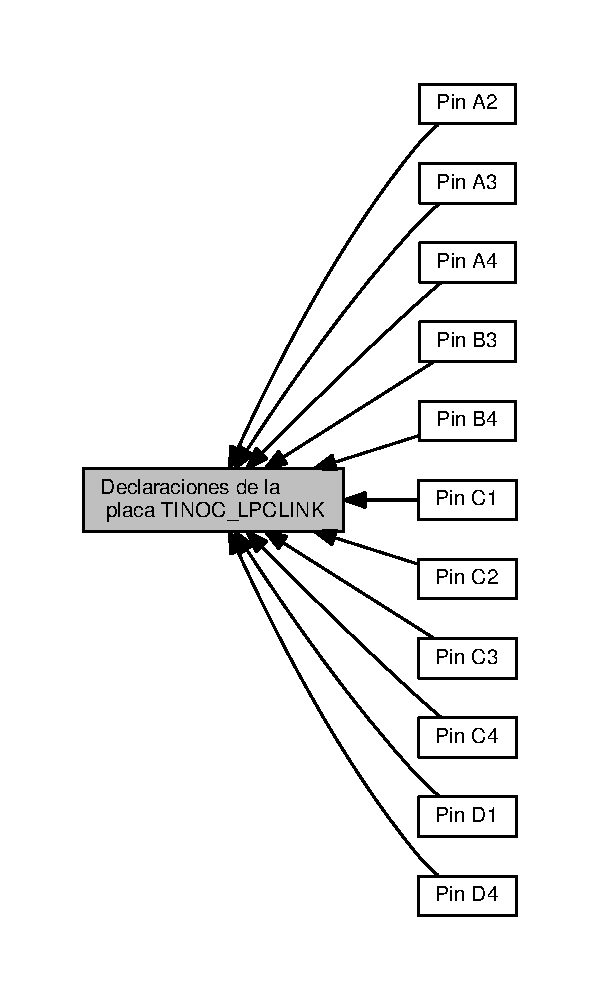
\includegraphics[width=288pt]{group___d_e_f_i_n_e_l_p_l_i_n_k}
\end{center}
\end{figure}
\subsection*{Modules}
\begin{DoxyCompactItemize}
\item 
\hyperlink{group___p_i_n_c1}{Pin C1}
\item 
\hyperlink{group___p_i_n_a2}{Pin A2}
\item 
\hyperlink{group___p_i_n_a3}{Pin A3}
\item 
\hyperlink{group___p_i_n_a4}{Pin A4}
\item 
\hyperlink{group___p_i_n_b4}{Pin B4}
\item 
\hyperlink{group___p_i_n_b3}{Pin B3}
\item 
\hyperlink{group___p_i_n_c4}{Pin C4}
\item 
\hyperlink{group___p_i_n_c3}{Pin C3}
\item 
\hyperlink{group___p_i_n_d4}{Pin D4}
\item 
\hyperlink{group___p_i_n_c2}{Pin C2}
\item 
\hyperlink{group___p_i_n_d1}{Pin D1}
\end{DoxyCompactItemize}


\subsection{Detailed Description}
Constantes asignadas a los pines de la placa. 


\hypertarget{group___p_i_n_c1}{}\section{Pin C1}
\label{group___p_i_n_c1}\index{Pin C1@{Pin C1}}
Collaboration diagram for Pin C1\+:\nopagebreak
\begin{figure}[H]
\begin{center}
\leavevmode
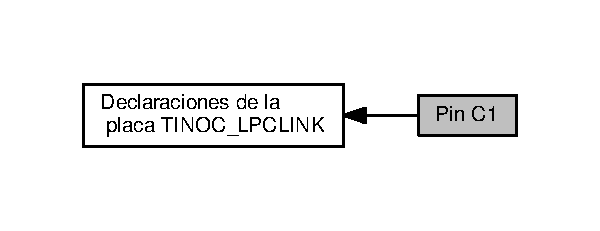
\includegraphics[width=288pt]{group___p_i_n_c1}
\end{center}
\end{figure}
\subsection*{Macros}
\begin{DoxyCompactItemize}
\item 
\#define \hyperlink{group___p_i_n_c1_gac6a22e60c760c46ea90fb0ebe728baa1}{L\+P\+C1102\+\_\+\+C1\+\_\+\+B\+IT}~( 1\+U\+L $<$$<$ 0\+U\+L )
\begin{DoxyCompactList}\small\item\em Defino el bit del puerto ocupado por C1. \end{DoxyCompactList}\item 
\#define \hyperlink{group___p_i_n_c1_ga858dd06436643c005fd1f54e54091e82}{L\+P\+C1102\+\_\+\+C1\+\_\+\+P\+O\+RT}~( 0 )
\begin{DoxyCompactList}\small\item\em Defino el port del puerto ocupado por C1. \end{DoxyCompactList}\item 
\#define \hyperlink{group___p_i_n_c1_gae77ae547e9f51dd166db043d9c2ab9ea}{L\+P\+C1102\+\_\+\+C1\+\_\+\+G\+P\+IO}~L\+P\+C\+\_\+\+G\+P\+I\+O0
\begin{DoxyCompactList}\small\item\em Defino el registro G\+P\+IO ocupado por C1. \end{DoxyCompactList}\end{DoxyCompactItemize}


\subsection{Detailed Description}


\subsection{Macro Definition Documentation}
\index{Pin C1@{Pin C1}!L\+P\+C1102\+\_\+\+C1\+\_\+\+B\+IT@{L\+P\+C1102\+\_\+\+C1\+\_\+\+B\+IT}}
\index{L\+P\+C1102\+\_\+\+C1\+\_\+\+B\+IT@{L\+P\+C1102\+\_\+\+C1\+\_\+\+B\+IT}!Pin C1@{Pin C1}}
\subsubsection[{\texorpdfstring{L\+P\+C1102\+\_\+\+C1\+\_\+\+B\+IT}{LPC1102_C1_BIT}}]{\setlength{\rightskip}{0pt plus 5cm}\#define L\+P\+C1102\+\_\+\+C1\+\_\+\+B\+IT~( 1\+U\+L $<$$<$ 0\+U\+L )}\hypertarget{group___p_i_n_c1_gac6a22e60c760c46ea90fb0ebe728baa1}{}\label{group___p_i_n_c1_gac6a22e60c760c46ea90fb0ebe728baa1}


Defino el bit del puerto ocupado por C1. 



Definition at line 28 of file tinoc\+\_\+lpclink.\+h.

\index{Pin C1@{Pin C1}!L\+P\+C1102\+\_\+\+C1\+\_\+\+G\+P\+IO@{L\+P\+C1102\+\_\+\+C1\+\_\+\+G\+P\+IO}}
\index{L\+P\+C1102\+\_\+\+C1\+\_\+\+G\+P\+IO@{L\+P\+C1102\+\_\+\+C1\+\_\+\+G\+P\+IO}!Pin C1@{Pin C1}}
\subsubsection[{\texorpdfstring{L\+P\+C1102\+\_\+\+C1\+\_\+\+G\+P\+IO}{LPC1102_C1_GPIO}}]{\setlength{\rightskip}{0pt plus 5cm}\#define L\+P\+C1102\+\_\+\+C1\+\_\+\+G\+P\+IO~L\+P\+C\+\_\+\+G\+P\+I\+O0}\hypertarget{group___p_i_n_c1_gae77ae547e9f51dd166db043d9c2ab9ea}{}\label{group___p_i_n_c1_gae77ae547e9f51dd166db043d9c2ab9ea}


Defino el registro G\+P\+IO ocupado por C1. 



Definition at line 32 of file tinoc\+\_\+lpclink.\+h.

\index{Pin C1@{Pin C1}!L\+P\+C1102\+\_\+\+C1\+\_\+\+P\+O\+RT@{L\+P\+C1102\+\_\+\+C1\+\_\+\+P\+O\+RT}}
\index{L\+P\+C1102\+\_\+\+C1\+\_\+\+P\+O\+RT@{L\+P\+C1102\+\_\+\+C1\+\_\+\+P\+O\+RT}!Pin C1@{Pin C1}}
\subsubsection[{\texorpdfstring{L\+P\+C1102\+\_\+\+C1\+\_\+\+P\+O\+RT}{LPC1102_C1_PORT}}]{\setlength{\rightskip}{0pt plus 5cm}\#define L\+P\+C1102\+\_\+\+C1\+\_\+\+P\+O\+RT~( 0 )}\hypertarget{group___p_i_n_c1_ga858dd06436643c005fd1f54e54091e82}{}\label{group___p_i_n_c1_ga858dd06436643c005fd1f54e54091e82}


Defino el port del puerto ocupado por C1. 



Definition at line 30 of file tinoc\+\_\+lpclink.\+h.


\hypertarget{group___p_i_n_a2}{}\section{Pin A2}
\label{group___p_i_n_a2}\index{Pin A2@{Pin A2}}
Collaboration diagram for Pin A2\+:\nopagebreak
\begin{figure}[H]
\begin{center}
\leavevmode
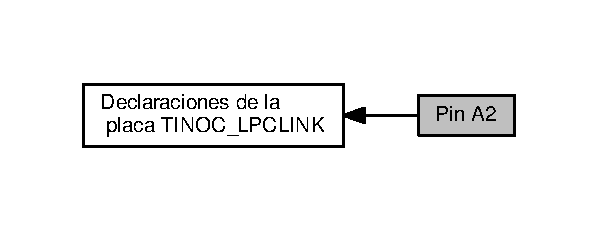
\includegraphics[width=287pt]{group___p_i_n_a2}
\end{center}
\end{figure}
\subsection*{Macros}
\begin{DoxyCompactItemize}
\item 
\#define \hyperlink{group___p_i_n_a2_ga468d2953fb3f21789957ee47f63e7c63}{L\+P\+C1102\+\_\+\+A2\+\_\+\+B\+IT}~( 1\+U\+L $<$$<$ 8\+U\+L )
\begin{DoxyCompactList}\small\item\em Defino el port y bit del puerto ocupado por A2. \end{DoxyCompactList}\item 
\#define \hyperlink{group___p_i_n_a2_gaab2a521ccd24403022ea360f4ba721bc}{L\+P\+C1102\+\_\+\+A2\+\_\+\+P\+O\+RT}~( 0 )
\begin{DoxyCompactList}\small\item\em Defino el port del puerto ocupado por A2. \end{DoxyCompactList}\item 
\#define \hyperlink{group___p_i_n_a2_ga0d6606e66c7be93dff6911f06846baea}{L\+P\+C1102\+\_\+\+A2\+\_\+\+G\+P\+IO}~L\+P\+C\+\_\+\+G\+P\+I\+O0
\begin{DoxyCompactList}\small\item\em Defino el registro G\+P\+IO ocupado por A2. \end{DoxyCompactList}\end{DoxyCompactItemize}


\subsection{Detailed Description}


\subsection{Macro Definition Documentation}
\index{Pin A2@{Pin A2}!L\+P\+C1102\+\_\+\+A2\+\_\+\+B\+IT@{L\+P\+C1102\+\_\+\+A2\+\_\+\+B\+IT}}
\index{L\+P\+C1102\+\_\+\+A2\+\_\+\+B\+IT@{L\+P\+C1102\+\_\+\+A2\+\_\+\+B\+IT}!Pin A2@{Pin A2}}
\subsubsection[{\texorpdfstring{L\+P\+C1102\+\_\+\+A2\+\_\+\+B\+IT}{LPC1102_A2_BIT}}]{\setlength{\rightskip}{0pt plus 5cm}\#define L\+P\+C1102\+\_\+\+A2\+\_\+\+B\+IT~( 1\+U\+L $<$$<$ 8\+U\+L )}\hypertarget{group___p_i_n_a2_ga468d2953fb3f21789957ee47f63e7c63}{}\label{group___p_i_n_a2_ga468d2953fb3f21789957ee47f63e7c63}


Defino el port y bit del puerto ocupado por A2. 



Definition at line 44 of file tinoc\+\_\+lpclink.\+h.

\index{Pin A2@{Pin A2}!L\+P\+C1102\+\_\+\+A2\+\_\+\+G\+P\+IO@{L\+P\+C1102\+\_\+\+A2\+\_\+\+G\+P\+IO}}
\index{L\+P\+C1102\+\_\+\+A2\+\_\+\+G\+P\+IO@{L\+P\+C1102\+\_\+\+A2\+\_\+\+G\+P\+IO}!Pin A2@{Pin A2}}
\subsubsection[{\texorpdfstring{L\+P\+C1102\+\_\+\+A2\+\_\+\+G\+P\+IO}{LPC1102_A2_GPIO}}]{\setlength{\rightskip}{0pt plus 5cm}\#define L\+P\+C1102\+\_\+\+A2\+\_\+\+G\+P\+IO~L\+P\+C\+\_\+\+G\+P\+I\+O0}\hypertarget{group___p_i_n_a2_ga0d6606e66c7be93dff6911f06846baea}{}\label{group___p_i_n_a2_ga0d6606e66c7be93dff6911f06846baea}


Defino el registro G\+P\+IO ocupado por A2. 



Definition at line 48 of file tinoc\+\_\+lpclink.\+h.

\index{Pin A2@{Pin A2}!L\+P\+C1102\+\_\+\+A2\+\_\+\+P\+O\+RT@{L\+P\+C1102\+\_\+\+A2\+\_\+\+P\+O\+RT}}
\index{L\+P\+C1102\+\_\+\+A2\+\_\+\+P\+O\+RT@{L\+P\+C1102\+\_\+\+A2\+\_\+\+P\+O\+RT}!Pin A2@{Pin A2}}
\subsubsection[{\texorpdfstring{L\+P\+C1102\+\_\+\+A2\+\_\+\+P\+O\+RT}{LPC1102_A2_PORT}}]{\setlength{\rightskip}{0pt plus 5cm}\#define L\+P\+C1102\+\_\+\+A2\+\_\+\+P\+O\+RT~( 0 )}\hypertarget{group___p_i_n_a2_gaab2a521ccd24403022ea360f4ba721bc}{}\label{group___p_i_n_a2_gaab2a521ccd24403022ea360f4ba721bc}


Defino el port del puerto ocupado por A2. 



Definition at line 46 of file tinoc\+\_\+lpclink.\+h.


\hypertarget{group___p_i_n_a3}{}\section{Pin A3}
\label{group___p_i_n_a3}\index{Pin A3@{Pin A3}}
Collaboration diagram for Pin A3\+:\nopagebreak
\begin{figure}[H]
\begin{center}
\leavevmode
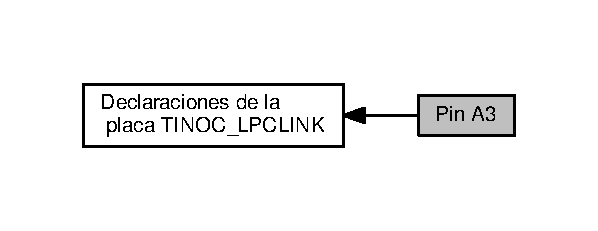
\includegraphics[width=287pt]{group___p_i_n_a3}
\end{center}
\end{figure}
\subsection*{Macros}
\begin{DoxyCompactItemize}
\item 
\#define \hyperlink{group___p_i_n_a3_ga42cf8ceb71f191c96859d8cbc3850b45}{L\+P\+C1102\+\_\+\+A3\+\_\+\+B\+IT}~( 1\+U\+L $<$$<$ 9\+U\+L )
\begin{DoxyCompactList}\small\item\em Defino el port y bit del puerto ocupado por A3. \end{DoxyCompactList}\item 
\#define \hyperlink{group___p_i_n_a3_ga5078bdf03502964ece28e1594df9a997}{L\+P\+C1102\+\_\+\+A3\+\_\+\+P\+O\+RT}~( 0 )
\begin{DoxyCompactList}\small\item\em Defino el port del puerto ocupado por A3. \end{DoxyCompactList}\item 
\#define \hyperlink{group___p_i_n_a3_ga10234a1267cbec06f769ec87765df961}{L\+P\+C1102\+\_\+\+A3\+\_\+\+G\+P\+IO}~L\+P\+C\+\_\+\+G\+P\+I\+O0
\begin{DoxyCompactList}\small\item\em Defino el registro G\+P\+IO ocupado por A3. \end{DoxyCompactList}\end{DoxyCompactItemize}


\subsection{Detailed Description}


\subsection{Macro Definition Documentation}
\index{Pin A3@{Pin A3}!L\+P\+C1102\+\_\+\+A3\+\_\+\+B\+IT@{L\+P\+C1102\+\_\+\+A3\+\_\+\+B\+IT}}
\index{L\+P\+C1102\+\_\+\+A3\+\_\+\+B\+IT@{L\+P\+C1102\+\_\+\+A3\+\_\+\+B\+IT}!Pin A3@{Pin A3}}
\subsubsection[{\texorpdfstring{L\+P\+C1102\+\_\+\+A3\+\_\+\+B\+IT}{LPC1102_A3_BIT}}]{\setlength{\rightskip}{0pt plus 5cm}\#define L\+P\+C1102\+\_\+\+A3\+\_\+\+B\+IT~( 1\+U\+L $<$$<$ 9\+U\+L )}\hypertarget{group___p_i_n_a3_ga42cf8ceb71f191c96859d8cbc3850b45}{}\label{group___p_i_n_a3_ga42cf8ceb71f191c96859d8cbc3850b45}


Defino el port y bit del puerto ocupado por A3. 



Definition at line 61 of file tinoc\+\_\+lpclink.\+h.

\index{Pin A3@{Pin A3}!L\+P\+C1102\+\_\+\+A3\+\_\+\+G\+P\+IO@{L\+P\+C1102\+\_\+\+A3\+\_\+\+G\+P\+IO}}
\index{L\+P\+C1102\+\_\+\+A3\+\_\+\+G\+P\+IO@{L\+P\+C1102\+\_\+\+A3\+\_\+\+G\+P\+IO}!Pin A3@{Pin A3}}
\subsubsection[{\texorpdfstring{L\+P\+C1102\+\_\+\+A3\+\_\+\+G\+P\+IO}{LPC1102_A3_GPIO}}]{\setlength{\rightskip}{0pt plus 5cm}\#define L\+P\+C1102\+\_\+\+A3\+\_\+\+G\+P\+IO~L\+P\+C\+\_\+\+G\+P\+I\+O0}\hypertarget{group___p_i_n_a3_ga10234a1267cbec06f769ec87765df961}{}\label{group___p_i_n_a3_ga10234a1267cbec06f769ec87765df961}


Defino el registro G\+P\+IO ocupado por A3. 



Definition at line 65 of file tinoc\+\_\+lpclink.\+h.

\index{Pin A3@{Pin A3}!L\+P\+C1102\+\_\+\+A3\+\_\+\+P\+O\+RT@{L\+P\+C1102\+\_\+\+A3\+\_\+\+P\+O\+RT}}
\index{L\+P\+C1102\+\_\+\+A3\+\_\+\+P\+O\+RT@{L\+P\+C1102\+\_\+\+A3\+\_\+\+P\+O\+RT}!Pin A3@{Pin A3}}
\subsubsection[{\texorpdfstring{L\+P\+C1102\+\_\+\+A3\+\_\+\+P\+O\+RT}{LPC1102_A3_PORT}}]{\setlength{\rightskip}{0pt plus 5cm}\#define L\+P\+C1102\+\_\+\+A3\+\_\+\+P\+O\+RT~( 0 )}\hypertarget{group___p_i_n_a3_ga5078bdf03502964ece28e1594df9a997}{}\label{group___p_i_n_a3_ga5078bdf03502964ece28e1594df9a997}


Defino el port del puerto ocupado por A3. 



Definition at line 63 of file tinoc\+\_\+lpclink.\+h.


\hypertarget{group___p_i_n_a4}{}\section{Pin A4}
\label{group___p_i_n_a4}\index{Pin A4@{Pin A4}}
Collaboration diagram for Pin A4\+:\nopagebreak
\begin{figure}[H]
\begin{center}
\leavevmode
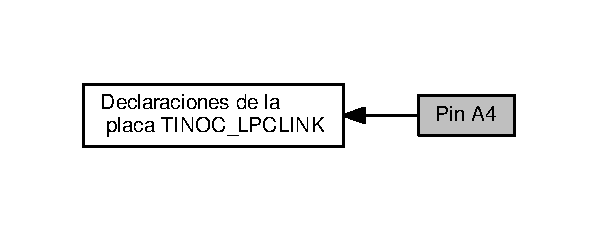
\includegraphics[width=287pt]{group___p_i_n_a4}
\end{center}
\end{figure}
\subsection*{Macros}
\begin{DoxyCompactItemize}
\item 
\#define \hyperlink{group___p_i_n_a4_ga23798f2c62b59f2710bbea33952bfcc8}{L\+P\+C1102\+\_\+\+A4\+\_\+\+B\+IT}~( 1\+U\+L $<$$<$ 10\+U\+L )
\begin{DoxyCompactList}\small\item\em Defino el port y bit del puerto ocupado por A4. \end{DoxyCompactList}\item 
\#define \hyperlink{group___p_i_n_a4_ga03e8289e4ef7c73d23799d95329c4d81}{L\+P\+C1102\+\_\+\+A4\+\_\+\+P\+O\+RT}~( 0 )
\begin{DoxyCompactList}\small\item\em Defino el port del puerto ocupado por A4. \end{DoxyCompactList}\item 
\#define \hyperlink{group___p_i_n_a4_ga958d137c3a737689f2158ceae5f0c7b1}{L\+P\+C1102\+\_\+\+A4\+\_\+\+G\+P\+IO}~L\+P\+C\+\_\+\+G\+P\+I\+O0
\begin{DoxyCompactList}\small\item\em Defino el registro G\+P\+IO ocupado por A4. \end{DoxyCompactList}\end{DoxyCompactItemize}


\subsection{Detailed Description}


\subsection{Macro Definition Documentation}
\index{Pin A4@{Pin A4}!L\+P\+C1102\+\_\+\+A4\+\_\+\+B\+IT@{L\+P\+C1102\+\_\+\+A4\+\_\+\+B\+IT}}
\index{L\+P\+C1102\+\_\+\+A4\+\_\+\+B\+IT@{L\+P\+C1102\+\_\+\+A4\+\_\+\+B\+IT}!Pin A4@{Pin A4}}
\subsubsection[{\texorpdfstring{L\+P\+C1102\+\_\+\+A4\+\_\+\+B\+IT}{LPC1102_A4_BIT}}]{\setlength{\rightskip}{0pt plus 5cm}\#define L\+P\+C1102\+\_\+\+A4\+\_\+\+B\+IT~( 1\+U\+L $<$$<$ 10\+U\+L )}\hypertarget{group___p_i_n_a4_ga23798f2c62b59f2710bbea33952bfcc8}{}\label{group___p_i_n_a4_ga23798f2c62b59f2710bbea33952bfcc8}


Defino el port y bit del puerto ocupado por A4. 



Definition at line 79 of file tinoc\+\_\+lpclink.\+h.

\index{Pin A4@{Pin A4}!L\+P\+C1102\+\_\+\+A4\+\_\+\+G\+P\+IO@{L\+P\+C1102\+\_\+\+A4\+\_\+\+G\+P\+IO}}
\index{L\+P\+C1102\+\_\+\+A4\+\_\+\+G\+P\+IO@{L\+P\+C1102\+\_\+\+A4\+\_\+\+G\+P\+IO}!Pin A4@{Pin A4}}
\subsubsection[{\texorpdfstring{L\+P\+C1102\+\_\+\+A4\+\_\+\+G\+P\+IO}{LPC1102_A4_GPIO}}]{\setlength{\rightskip}{0pt plus 5cm}\#define L\+P\+C1102\+\_\+\+A4\+\_\+\+G\+P\+IO~L\+P\+C\+\_\+\+G\+P\+I\+O0}\hypertarget{group___p_i_n_a4_ga958d137c3a737689f2158ceae5f0c7b1}{}\label{group___p_i_n_a4_ga958d137c3a737689f2158ceae5f0c7b1}


Defino el registro G\+P\+IO ocupado por A4. 



Definition at line 83 of file tinoc\+\_\+lpclink.\+h.

\index{Pin A4@{Pin A4}!L\+P\+C1102\+\_\+\+A4\+\_\+\+P\+O\+RT@{L\+P\+C1102\+\_\+\+A4\+\_\+\+P\+O\+RT}}
\index{L\+P\+C1102\+\_\+\+A4\+\_\+\+P\+O\+RT@{L\+P\+C1102\+\_\+\+A4\+\_\+\+P\+O\+RT}!Pin A4@{Pin A4}}
\subsubsection[{\texorpdfstring{L\+P\+C1102\+\_\+\+A4\+\_\+\+P\+O\+RT}{LPC1102_A4_PORT}}]{\setlength{\rightskip}{0pt plus 5cm}\#define L\+P\+C1102\+\_\+\+A4\+\_\+\+P\+O\+RT~( 0 )}\hypertarget{group___p_i_n_a4_ga03e8289e4ef7c73d23799d95329c4d81}{}\label{group___p_i_n_a4_ga03e8289e4ef7c73d23799d95329c4d81}


Defino el port del puerto ocupado por A4. 



Definition at line 81 of file tinoc\+\_\+lpclink.\+h.


\hypertarget{group___p_i_n_b4}{}\section{Pin B4}
\label{group___p_i_n_b4}\index{Pin B4@{Pin B4}}
Collaboration diagram for Pin B4\+:\nopagebreak
\begin{figure}[H]
\begin{center}
\leavevmode
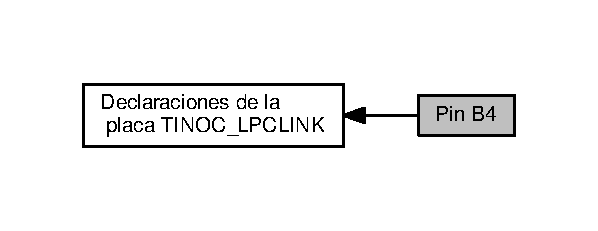
\includegraphics[width=287pt]{group___p_i_n_b4}
\end{center}
\end{figure}
\subsection*{Macros}
\begin{DoxyCompactItemize}
\item 
\#define \hyperlink{group___p_i_n_b4_gabd8ff8e5626973a20825ed09a23f6c6e}{L\+P\+C1102\+\_\+\+B4\+\_\+\+B\+IT}~( 1\+U\+L $<$$<$ 11\+U\+L )
\begin{DoxyCompactList}\small\item\em Defino el port y bit del puerto ocupado por B4. \end{DoxyCompactList}\item 
\#define \hyperlink{group___p_i_n_b4_gaa66d572d746828aa3a56c00b2388aa61}{L\+P\+C1102\+\_\+\+B4\+\_\+\+P\+O\+RT}~( 0 )
\begin{DoxyCompactList}\small\item\em Defino el port del puerto ocupado por B4. \end{DoxyCompactList}\item 
\#define \hyperlink{group___p_i_n_b4_gacbcccf71d8c04a772bba72aeca46284a}{L\+P\+C1102\+\_\+\+B4\+\_\+\+G\+P\+IO}~L\+P\+C\+\_\+\+G\+P\+I\+O0
\begin{DoxyCompactList}\small\item\em Defino el registro G\+P\+IO ocupado por B4. \end{DoxyCompactList}\end{DoxyCompactItemize}


\subsection{Detailed Description}


\subsection{Macro Definition Documentation}
\index{Pin B4@{Pin B4}!L\+P\+C1102\+\_\+\+B4\+\_\+\+B\+IT@{L\+P\+C1102\+\_\+\+B4\+\_\+\+B\+IT}}
\index{L\+P\+C1102\+\_\+\+B4\+\_\+\+B\+IT@{L\+P\+C1102\+\_\+\+B4\+\_\+\+B\+IT}!Pin B4@{Pin B4}}
\subsubsection[{\texorpdfstring{L\+P\+C1102\+\_\+\+B4\+\_\+\+B\+IT}{LPC1102_B4_BIT}}]{\setlength{\rightskip}{0pt plus 5cm}\#define L\+P\+C1102\+\_\+\+B4\+\_\+\+B\+IT~( 1\+U\+L $<$$<$ 11\+U\+L )}\hypertarget{group___p_i_n_b4_gabd8ff8e5626973a20825ed09a23f6c6e}{}\label{group___p_i_n_b4_gabd8ff8e5626973a20825ed09a23f6c6e}


Defino el port y bit del puerto ocupado por B4. 



Definition at line 95 of file tinoc\+\_\+lpclink.\+h.

\index{Pin B4@{Pin B4}!L\+P\+C1102\+\_\+\+B4\+\_\+\+G\+P\+IO@{L\+P\+C1102\+\_\+\+B4\+\_\+\+G\+P\+IO}}
\index{L\+P\+C1102\+\_\+\+B4\+\_\+\+G\+P\+IO@{L\+P\+C1102\+\_\+\+B4\+\_\+\+G\+P\+IO}!Pin B4@{Pin B4}}
\subsubsection[{\texorpdfstring{L\+P\+C1102\+\_\+\+B4\+\_\+\+G\+P\+IO}{LPC1102_B4_GPIO}}]{\setlength{\rightskip}{0pt plus 5cm}\#define L\+P\+C1102\+\_\+\+B4\+\_\+\+G\+P\+IO~L\+P\+C\+\_\+\+G\+P\+I\+O0}\hypertarget{group___p_i_n_b4_gacbcccf71d8c04a772bba72aeca46284a}{}\label{group___p_i_n_b4_gacbcccf71d8c04a772bba72aeca46284a}


Defino el registro G\+P\+IO ocupado por B4. 



Definition at line 99 of file tinoc\+\_\+lpclink.\+h.

\index{Pin B4@{Pin B4}!L\+P\+C1102\+\_\+\+B4\+\_\+\+P\+O\+RT@{L\+P\+C1102\+\_\+\+B4\+\_\+\+P\+O\+RT}}
\index{L\+P\+C1102\+\_\+\+B4\+\_\+\+P\+O\+RT@{L\+P\+C1102\+\_\+\+B4\+\_\+\+P\+O\+RT}!Pin B4@{Pin B4}}
\subsubsection[{\texorpdfstring{L\+P\+C1102\+\_\+\+B4\+\_\+\+P\+O\+RT}{LPC1102_B4_PORT}}]{\setlength{\rightskip}{0pt plus 5cm}\#define L\+P\+C1102\+\_\+\+B4\+\_\+\+P\+O\+RT~( 0 )}\hypertarget{group___p_i_n_b4_gaa66d572d746828aa3a56c00b2388aa61}{}\label{group___p_i_n_b4_gaa66d572d746828aa3a56c00b2388aa61}


Defino el port del puerto ocupado por B4. 



Definition at line 97 of file tinoc\+\_\+lpclink.\+h.


\hypertarget{group___p_i_n_b3}{}\section{Pin B3}
\label{group___p_i_n_b3}\index{Pin B3@{Pin B3}}
Collaboration diagram for Pin B3\+:\nopagebreak
\begin{figure}[H]
\begin{center}
\leavevmode
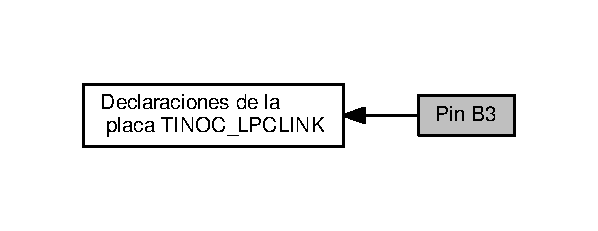
\includegraphics[width=287pt]{group___p_i_n_b3}
\end{center}
\end{figure}
\subsection*{Macros}
\begin{DoxyCompactItemize}
\item 
\#define \hyperlink{group___p_i_n_b3_ga39bcaf57d33e1054d42f18cdb09ee3f3}{L\+P\+C1102\+\_\+\+B3\+\_\+\+B\+IT}~( 1\+U\+L $<$$<$ 0\+U\+L )
\begin{DoxyCompactList}\small\item\em Defino el port y bit del puerto ocupado por B3. \end{DoxyCompactList}\item 
\#define \hyperlink{group___p_i_n_b3_ga2d2cd4b200ff348a009d8893cbeefaf8}{L\+P\+C1102\+\_\+\+B3\+\_\+\+P\+O\+RT}~( 1 )
\begin{DoxyCompactList}\small\item\em Defino el port del puerto ocupado por B3. \end{DoxyCompactList}\item 
\#define \hyperlink{group___p_i_n_b3_gab894d5a6e82d3bb1548150fa1f903c84}{L\+P\+C1102\+\_\+\+B3\+\_\+\+G\+P\+IO}~L\+P\+C\+\_\+\+G\+P\+I\+O1
\begin{DoxyCompactList}\small\item\em Defino el registro G\+P\+IO ocupado por B3. \end{DoxyCompactList}\end{DoxyCompactItemize}


\subsection{Detailed Description}


\subsection{Macro Definition Documentation}
\index{Pin B3@{Pin B3}!L\+P\+C1102\+\_\+\+B3\+\_\+\+B\+IT@{L\+P\+C1102\+\_\+\+B3\+\_\+\+B\+IT}}
\index{L\+P\+C1102\+\_\+\+B3\+\_\+\+B\+IT@{L\+P\+C1102\+\_\+\+B3\+\_\+\+B\+IT}!Pin B3@{Pin B3}}
\subsubsection[{\texorpdfstring{L\+P\+C1102\+\_\+\+B3\+\_\+\+B\+IT}{LPC1102_B3_BIT}}]{\setlength{\rightskip}{0pt plus 5cm}\#define L\+P\+C1102\+\_\+\+B3\+\_\+\+B\+IT~( 1\+U\+L $<$$<$ 0\+U\+L )}\hypertarget{group___p_i_n_b3_ga39bcaf57d33e1054d42f18cdb09ee3f3}{}\label{group___p_i_n_b3_ga39bcaf57d33e1054d42f18cdb09ee3f3}


Defino el port y bit del puerto ocupado por B3. 



Definition at line 112 of file tinoc\+\_\+lpclink.\+h.

\index{Pin B3@{Pin B3}!L\+P\+C1102\+\_\+\+B3\+\_\+\+G\+P\+IO@{L\+P\+C1102\+\_\+\+B3\+\_\+\+G\+P\+IO}}
\index{L\+P\+C1102\+\_\+\+B3\+\_\+\+G\+P\+IO@{L\+P\+C1102\+\_\+\+B3\+\_\+\+G\+P\+IO}!Pin B3@{Pin B3}}
\subsubsection[{\texorpdfstring{L\+P\+C1102\+\_\+\+B3\+\_\+\+G\+P\+IO}{LPC1102_B3_GPIO}}]{\setlength{\rightskip}{0pt plus 5cm}\#define L\+P\+C1102\+\_\+\+B3\+\_\+\+G\+P\+IO~L\+P\+C\+\_\+\+G\+P\+I\+O1}\hypertarget{group___p_i_n_b3_gab894d5a6e82d3bb1548150fa1f903c84}{}\label{group___p_i_n_b3_gab894d5a6e82d3bb1548150fa1f903c84}


Defino el registro G\+P\+IO ocupado por B3. 



Definition at line 116 of file tinoc\+\_\+lpclink.\+h.

\index{Pin B3@{Pin B3}!L\+P\+C1102\+\_\+\+B3\+\_\+\+P\+O\+RT@{L\+P\+C1102\+\_\+\+B3\+\_\+\+P\+O\+RT}}
\index{L\+P\+C1102\+\_\+\+B3\+\_\+\+P\+O\+RT@{L\+P\+C1102\+\_\+\+B3\+\_\+\+P\+O\+RT}!Pin B3@{Pin B3}}
\subsubsection[{\texorpdfstring{L\+P\+C1102\+\_\+\+B3\+\_\+\+P\+O\+RT}{LPC1102_B3_PORT}}]{\setlength{\rightskip}{0pt plus 5cm}\#define L\+P\+C1102\+\_\+\+B3\+\_\+\+P\+O\+RT~( 1 )}\hypertarget{group___p_i_n_b3_ga2d2cd4b200ff348a009d8893cbeefaf8}{}\label{group___p_i_n_b3_ga2d2cd4b200ff348a009d8893cbeefaf8}


Defino el port del puerto ocupado por B3. 



Definition at line 114 of file tinoc\+\_\+lpclink.\+h.


\hypertarget{group___p_i_n_c4}{}\section{Pin C4}
\label{group___p_i_n_c4}\index{Pin C4@{Pin C4}}
Collaboration diagram for Pin C4\+:\nopagebreak
\begin{figure}[H]
\begin{center}
\leavevmode
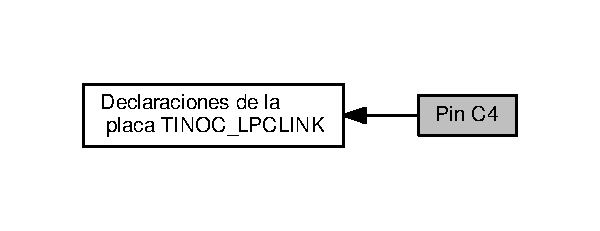
\includegraphics[width=288pt]{group___p_i_n_c4}
\end{center}
\end{figure}
\subsection*{Macros}
\begin{DoxyCompactItemize}
\item 
\#define \hyperlink{group___p_i_n_c4_ga6634a8d3b9fbbf4a90aa74fe9173de32}{L\+P\+C1102\+\_\+\+C4\+\_\+\+B\+IT}~( 1\+U\+L $<$$<$ 1\+U\+L )
\begin{DoxyCompactList}\small\item\em Defino el port y bit del puerto ocupado por C4. \end{DoxyCompactList}\item 
\#define \hyperlink{group___p_i_n_c4_gacd93f24da1e5789ee014bc52402d0bb5}{L\+P\+C1102\+\_\+\+C4\+\_\+\+P\+O\+RT}~( 1 )
\begin{DoxyCompactList}\small\item\em Defino el port del puerto ocupado por C4. \end{DoxyCompactList}\item 
\#define \hyperlink{group___p_i_n_c4_gad0c89c3a531c5e51f42bd3bcadd0c214}{L\+P\+C1102\+\_\+\+C4\+\_\+\+G\+P\+IO}~L\+P\+C\+\_\+\+G\+P\+I\+O1
\begin{DoxyCompactList}\small\item\em Defino el registro G\+P\+IO ocupado por C4. \end{DoxyCompactList}\end{DoxyCompactItemize}


\subsection{Detailed Description}


\subsection{Macro Definition Documentation}
\index{Pin C4@{Pin C4}!L\+P\+C1102\+\_\+\+C4\+\_\+\+B\+IT@{L\+P\+C1102\+\_\+\+C4\+\_\+\+B\+IT}}
\index{L\+P\+C1102\+\_\+\+C4\+\_\+\+B\+IT@{L\+P\+C1102\+\_\+\+C4\+\_\+\+B\+IT}!Pin C4@{Pin C4}}
\subsubsection[{\texorpdfstring{L\+P\+C1102\+\_\+\+C4\+\_\+\+B\+IT}{LPC1102_C4_BIT}}]{\setlength{\rightskip}{0pt plus 5cm}\#define L\+P\+C1102\+\_\+\+C4\+\_\+\+B\+IT~( 1\+U\+L $<$$<$ 1\+U\+L )}\hypertarget{group___p_i_n_c4_ga6634a8d3b9fbbf4a90aa74fe9173de32}{}\label{group___p_i_n_c4_ga6634a8d3b9fbbf4a90aa74fe9173de32}


Defino el port y bit del puerto ocupado por C4. 



Definition at line 128 of file tinoc\+\_\+lpclink.\+h.

\index{Pin C4@{Pin C4}!L\+P\+C1102\+\_\+\+C4\+\_\+\+G\+P\+IO@{L\+P\+C1102\+\_\+\+C4\+\_\+\+G\+P\+IO}}
\index{L\+P\+C1102\+\_\+\+C4\+\_\+\+G\+P\+IO@{L\+P\+C1102\+\_\+\+C4\+\_\+\+G\+P\+IO}!Pin C4@{Pin C4}}
\subsubsection[{\texorpdfstring{L\+P\+C1102\+\_\+\+C4\+\_\+\+G\+P\+IO}{LPC1102_C4_GPIO}}]{\setlength{\rightskip}{0pt plus 5cm}\#define L\+P\+C1102\+\_\+\+C4\+\_\+\+G\+P\+IO~L\+P\+C\+\_\+\+G\+P\+I\+O1}\hypertarget{group___p_i_n_c4_gad0c89c3a531c5e51f42bd3bcadd0c214}{}\label{group___p_i_n_c4_gad0c89c3a531c5e51f42bd3bcadd0c214}


Defino el registro G\+P\+IO ocupado por C4. 



Definition at line 132 of file tinoc\+\_\+lpclink.\+h.

\index{Pin C4@{Pin C4}!L\+P\+C1102\+\_\+\+C4\+\_\+\+P\+O\+RT@{L\+P\+C1102\+\_\+\+C4\+\_\+\+P\+O\+RT}}
\index{L\+P\+C1102\+\_\+\+C4\+\_\+\+P\+O\+RT@{L\+P\+C1102\+\_\+\+C4\+\_\+\+P\+O\+RT}!Pin C4@{Pin C4}}
\subsubsection[{\texorpdfstring{L\+P\+C1102\+\_\+\+C4\+\_\+\+P\+O\+RT}{LPC1102_C4_PORT}}]{\setlength{\rightskip}{0pt plus 5cm}\#define L\+P\+C1102\+\_\+\+C4\+\_\+\+P\+O\+RT~( 1 )}\hypertarget{group___p_i_n_c4_gacd93f24da1e5789ee014bc52402d0bb5}{}\label{group___p_i_n_c4_gacd93f24da1e5789ee014bc52402d0bb5}


Defino el port del puerto ocupado por C4. 



Definition at line 130 of file tinoc\+\_\+lpclink.\+h.


\hypertarget{group___p_i_n_c3}{}\section{Pin C3}
\label{group___p_i_n_c3}\index{Pin C3@{Pin C3}}
Collaboration diagram for Pin C3\+:\nopagebreak
\begin{figure}[H]
\begin{center}
\leavevmode
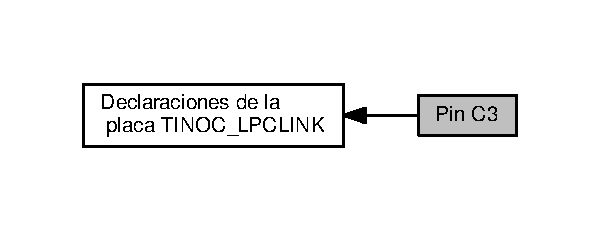
\includegraphics[width=288pt]{group___p_i_n_c3}
\end{center}
\end{figure}
\subsection*{Macros}
\begin{DoxyCompactItemize}
\item 
\#define \hyperlink{group___p_i_n_c3_ga9d9663e63d678743aeb834bbff7c7aed}{L\+P\+C1102\+\_\+\+C3\+\_\+\+B\+IT}~( 1\+U\+L $<$$<$ 2\+U\+L )
\begin{DoxyCompactList}\small\item\em Defino el port y bit del puerto ocupado por C3. \end{DoxyCompactList}\item 
\#define \hyperlink{group___p_i_n_c3_ga7a5850ce0680199eef3742f80e5e8c85}{L\+P\+C1102\+\_\+\+C3\+\_\+\+P\+O\+RT}~( 1 )
\begin{DoxyCompactList}\small\item\em Defino el port del puerto ocupado por C3. \end{DoxyCompactList}\item 
\#define \hyperlink{group___p_i_n_c3_gaee995322210bd5ce83ebe39b13dbd6bf}{L\+P\+C1102\+\_\+\+C3\+\_\+\+G\+P\+IO}~L\+P\+C\+\_\+\+G\+P\+I\+O1
\begin{DoxyCompactList}\small\item\em Defino el registro G\+P\+IO ocupado por C3. \end{DoxyCompactList}\end{DoxyCompactItemize}


\subsection{Detailed Description}


\subsection{Macro Definition Documentation}
\index{Pin C3@{Pin C3}!L\+P\+C1102\+\_\+\+C3\+\_\+\+B\+IT@{L\+P\+C1102\+\_\+\+C3\+\_\+\+B\+IT}}
\index{L\+P\+C1102\+\_\+\+C3\+\_\+\+B\+IT@{L\+P\+C1102\+\_\+\+C3\+\_\+\+B\+IT}!Pin C3@{Pin C3}}
\subsubsection[{\texorpdfstring{L\+P\+C1102\+\_\+\+C3\+\_\+\+B\+IT}{LPC1102_C3_BIT}}]{\setlength{\rightskip}{0pt plus 5cm}\#define L\+P\+C1102\+\_\+\+C3\+\_\+\+B\+IT~( 1\+U\+L $<$$<$ 2\+U\+L )}\hypertarget{group___p_i_n_c3_ga9d9663e63d678743aeb834bbff7c7aed}{}\label{group___p_i_n_c3_ga9d9663e63d678743aeb834bbff7c7aed}


Defino el port y bit del puerto ocupado por C3. 



Definition at line 144 of file tinoc\+\_\+lpclink.\+h.

\index{Pin C3@{Pin C3}!L\+P\+C1102\+\_\+\+C3\+\_\+\+G\+P\+IO@{L\+P\+C1102\+\_\+\+C3\+\_\+\+G\+P\+IO}}
\index{L\+P\+C1102\+\_\+\+C3\+\_\+\+G\+P\+IO@{L\+P\+C1102\+\_\+\+C3\+\_\+\+G\+P\+IO}!Pin C3@{Pin C3}}
\subsubsection[{\texorpdfstring{L\+P\+C1102\+\_\+\+C3\+\_\+\+G\+P\+IO}{LPC1102_C3_GPIO}}]{\setlength{\rightskip}{0pt plus 5cm}\#define L\+P\+C1102\+\_\+\+C3\+\_\+\+G\+P\+IO~L\+P\+C\+\_\+\+G\+P\+I\+O1}\hypertarget{group___p_i_n_c3_gaee995322210bd5ce83ebe39b13dbd6bf}{}\label{group___p_i_n_c3_gaee995322210bd5ce83ebe39b13dbd6bf}


Defino el registro G\+P\+IO ocupado por C3. 



Definition at line 148 of file tinoc\+\_\+lpclink.\+h.

\index{Pin C3@{Pin C3}!L\+P\+C1102\+\_\+\+C3\+\_\+\+P\+O\+RT@{L\+P\+C1102\+\_\+\+C3\+\_\+\+P\+O\+RT}}
\index{L\+P\+C1102\+\_\+\+C3\+\_\+\+P\+O\+RT@{L\+P\+C1102\+\_\+\+C3\+\_\+\+P\+O\+RT}!Pin C3@{Pin C3}}
\subsubsection[{\texorpdfstring{L\+P\+C1102\+\_\+\+C3\+\_\+\+P\+O\+RT}{LPC1102_C3_PORT}}]{\setlength{\rightskip}{0pt plus 5cm}\#define L\+P\+C1102\+\_\+\+C3\+\_\+\+P\+O\+RT~( 1 )}\hypertarget{group___p_i_n_c3_ga7a5850ce0680199eef3742f80e5e8c85}{}\label{group___p_i_n_c3_ga7a5850ce0680199eef3742f80e5e8c85}


Defino el port del puerto ocupado por C3. 



Definition at line 146 of file tinoc\+\_\+lpclink.\+h.


\hypertarget{group___p_i_n_d4}{}\section{Pin D4}
\label{group___p_i_n_d4}\index{Pin D4@{Pin D4}}
Collaboration diagram for Pin D4\+:\nopagebreak
\begin{figure}[H]
\begin{center}
\leavevmode
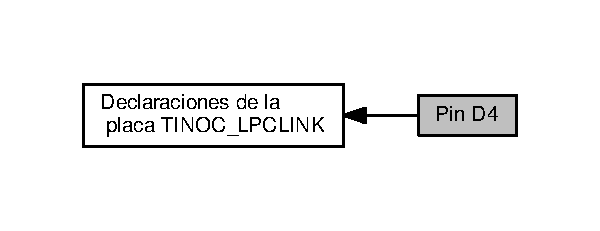
\includegraphics[width=288pt]{group___p_i_n_d4}
\end{center}
\end{figure}
\subsection*{Macros}
\begin{DoxyCompactItemize}
\item 
\#define \hyperlink{group___p_i_n_d4_ga9654c36aa00f501fb2cec682f6aa84c4}{L\+P\+C1102\+\_\+\+D4\+\_\+\+B\+IT}~( 1\+U\+L $<$$<$ 3\+U\+L )
\begin{DoxyCompactList}\small\item\em Defino el port y bit del puerto ocupado por D4. \end{DoxyCompactList}\item 
\#define \hyperlink{group___p_i_n_d4_ga58a788705aa9b7850deb5fa19cfd856c}{L\+P\+C1102\+\_\+\+D4\+\_\+\+P\+O\+RT}~( 1 )
\begin{DoxyCompactList}\small\item\em Defino el port del puerto ocupado por D4. \end{DoxyCompactList}\item 
\#define \hyperlink{group___p_i_n_d4_ga6ca2b1173d8c6e4ca72a10d780fdfd80}{L\+P\+C1102\+\_\+\+D4\+\_\+\+G\+P\+IO}~L\+P\+C\+\_\+\+G\+P\+I\+O1
\begin{DoxyCompactList}\small\item\em Defino el registro G\+P\+IO ocupado por D4. \end{DoxyCompactList}\end{DoxyCompactItemize}


\subsection{Detailed Description}


\subsection{Macro Definition Documentation}
\index{Pin D4@{Pin D4}!L\+P\+C1102\+\_\+\+D4\+\_\+\+B\+IT@{L\+P\+C1102\+\_\+\+D4\+\_\+\+B\+IT}}
\index{L\+P\+C1102\+\_\+\+D4\+\_\+\+B\+IT@{L\+P\+C1102\+\_\+\+D4\+\_\+\+B\+IT}!Pin D4@{Pin D4}}
\subsubsection[{\texorpdfstring{L\+P\+C1102\+\_\+\+D4\+\_\+\+B\+IT}{LPC1102_D4_BIT}}]{\setlength{\rightskip}{0pt plus 5cm}\#define L\+P\+C1102\+\_\+\+D4\+\_\+\+B\+IT~( 1\+U\+L $<$$<$ 3\+U\+L )}\hypertarget{group___p_i_n_d4_ga9654c36aa00f501fb2cec682f6aa84c4}{}\label{group___p_i_n_d4_ga9654c36aa00f501fb2cec682f6aa84c4}


Defino el port y bit del puerto ocupado por D4. 



Definition at line 160 of file tinoc\+\_\+lpclink.\+h.

\index{Pin D4@{Pin D4}!L\+P\+C1102\+\_\+\+D4\+\_\+\+G\+P\+IO@{L\+P\+C1102\+\_\+\+D4\+\_\+\+G\+P\+IO}}
\index{L\+P\+C1102\+\_\+\+D4\+\_\+\+G\+P\+IO@{L\+P\+C1102\+\_\+\+D4\+\_\+\+G\+P\+IO}!Pin D4@{Pin D4}}
\subsubsection[{\texorpdfstring{L\+P\+C1102\+\_\+\+D4\+\_\+\+G\+P\+IO}{LPC1102_D4_GPIO}}]{\setlength{\rightskip}{0pt plus 5cm}\#define L\+P\+C1102\+\_\+\+D4\+\_\+\+G\+P\+IO~L\+P\+C\+\_\+\+G\+P\+I\+O1}\hypertarget{group___p_i_n_d4_ga6ca2b1173d8c6e4ca72a10d780fdfd80}{}\label{group___p_i_n_d4_ga6ca2b1173d8c6e4ca72a10d780fdfd80}


Defino el registro G\+P\+IO ocupado por D4. 



Definition at line 164 of file tinoc\+\_\+lpclink.\+h.

\index{Pin D4@{Pin D4}!L\+P\+C1102\+\_\+\+D4\+\_\+\+P\+O\+RT@{L\+P\+C1102\+\_\+\+D4\+\_\+\+P\+O\+RT}}
\index{L\+P\+C1102\+\_\+\+D4\+\_\+\+P\+O\+RT@{L\+P\+C1102\+\_\+\+D4\+\_\+\+P\+O\+RT}!Pin D4@{Pin D4}}
\subsubsection[{\texorpdfstring{L\+P\+C1102\+\_\+\+D4\+\_\+\+P\+O\+RT}{LPC1102_D4_PORT}}]{\setlength{\rightskip}{0pt plus 5cm}\#define L\+P\+C1102\+\_\+\+D4\+\_\+\+P\+O\+RT~( 1 )}\hypertarget{group___p_i_n_d4_ga58a788705aa9b7850deb5fa19cfd856c}{}\label{group___p_i_n_d4_ga58a788705aa9b7850deb5fa19cfd856c}


Defino el port del puerto ocupado por D4. 



Definition at line 162 of file tinoc\+\_\+lpclink.\+h.


\hypertarget{group___p_i_n_c2}{}\section{Pin C2}
\label{group___p_i_n_c2}\index{Pin C2@{Pin C2}}
Collaboration diagram for Pin C2\+:\nopagebreak
\begin{figure}[H]
\begin{center}
\leavevmode
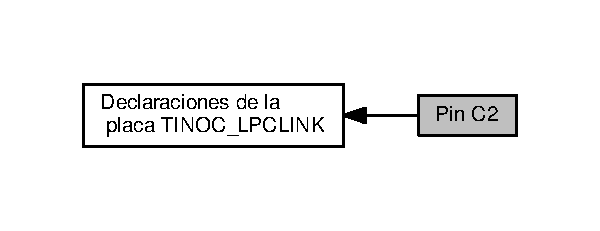
\includegraphics[width=288pt]{group___p_i_n_c2}
\end{center}
\end{figure}
\subsection*{Macros}
\begin{DoxyCompactItemize}
\item 
\#define \hyperlink{group___p_i_n_c2_gabce4949f6b4b70f2239eb55ac429559b}{L\+P\+C1102\+\_\+\+C2\+\_\+\+B\+IT}~( 1\+U\+L $<$$<$ 6\+U\+L )
\begin{DoxyCompactList}\small\item\em Defino el port y bit del puerto ocupado por C2. \end{DoxyCompactList}\item 
\#define \hyperlink{group___p_i_n_c2_ga50df256c7cdc2b746d468ab4ce10df85}{L\+P\+C1102\+\_\+\+C2\+\_\+\+P\+O\+RT}~( 1 )
\begin{DoxyCompactList}\small\item\em Defino el port del puerto ocupado por C2. \end{DoxyCompactList}\item 
\#define \hyperlink{group___p_i_n_c2_ga88c5ae9982021d59bd43dc9b9b22d1b9}{L\+P\+C1102\+\_\+\+C2\+\_\+\+G\+P\+IO}~L\+P\+C\+\_\+\+G\+P\+I\+O1
\begin{DoxyCompactList}\small\item\em Defino el registro G\+P\+IO ocupado por C2. \end{DoxyCompactList}\end{DoxyCompactItemize}


\subsection{Detailed Description}


\subsection{Macro Definition Documentation}
\index{Pin C2@{Pin C2}!L\+P\+C1102\+\_\+\+C2\+\_\+\+B\+IT@{L\+P\+C1102\+\_\+\+C2\+\_\+\+B\+IT}}
\index{L\+P\+C1102\+\_\+\+C2\+\_\+\+B\+IT@{L\+P\+C1102\+\_\+\+C2\+\_\+\+B\+IT}!Pin C2@{Pin C2}}
\subsubsection[{\texorpdfstring{L\+P\+C1102\+\_\+\+C2\+\_\+\+B\+IT}{LPC1102_C2_BIT}}]{\setlength{\rightskip}{0pt plus 5cm}\#define L\+P\+C1102\+\_\+\+C2\+\_\+\+B\+IT~( 1\+U\+L $<$$<$ 6\+U\+L )}\hypertarget{group___p_i_n_c2_gabce4949f6b4b70f2239eb55ac429559b}{}\label{group___p_i_n_c2_gabce4949f6b4b70f2239eb55ac429559b}


Defino el port y bit del puerto ocupado por C2. 



Definition at line 176 of file tinoc\+\_\+lpclink.\+h.

\index{Pin C2@{Pin C2}!L\+P\+C1102\+\_\+\+C2\+\_\+\+G\+P\+IO@{L\+P\+C1102\+\_\+\+C2\+\_\+\+G\+P\+IO}}
\index{L\+P\+C1102\+\_\+\+C2\+\_\+\+G\+P\+IO@{L\+P\+C1102\+\_\+\+C2\+\_\+\+G\+P\+IO}!Pin C2@{Pin C2}}
\subsubsection[{\texorpdfstring{L\+P\+C1102\+\_\+\+C2\+\_\+\+G\+P\+IO}{LPC1102_C2_GPIO}}]{\setlength{\rightskip}{0pt plus 5cm}\#define L\+P\+C1102\+\_\+\+C2\+\_\+\+G\+P\+IO~L\+P\+C\+\_\+\+G\+P\+I\+O1}\hypertarget{group___p_i_n_c2_ga88c5ae9982021d59bd43dc9b9b22d1b9}{}\label{group___p_i_n_c2_ga88c5ae9982021d59bd43dc9b9b22d1b9}


Defino el registro G\+P\+IO ocupado por C2. 



Definition at line 180 of file tinoc\+\_\+lpclink.\+h.

\index{Pin C2@{Pin C2}!L\+P\+C1102\+\_\+\+C2\+\_\+\+P\+O\+RT@{L\+P\+C1102\+\_\+\+C2\+\_\+\+P\+O\+RT}}
\index{L\+P\+C1102\+\_\+\+C2\+\_\+\+P\+O\+RT@{L\+P\+C1102\+\_\+\+C2\+\_\+\+P\+O\+RT}!Pin C2@{Pin C2}}
\subsubsection[{\texorpdfstring{L\+P\+C1102\+\_\+\+C2\+\_\+\+P\+O\+RT}{LPC1102_C2_PORT}}]{\setlength{\rightskip}{0pt plus 5cm}\#define L\+P\+C1102\+\_\+\+C2\+\_\+\+P\+O\+RT~( 1 )}\hypertarget{group___p_i_n_c2_ga50df256c7cdc2b746d468ab4ce10df85}{}\label{group___p_i_n_c2_ga50df256c7cdc2b746d468ab4ce10df85}


Defino el port del puerto ocupado por C2. 



Definition at line 178 of file tinoc\+\_\+lpclink.\+h.


\hypertarget{group___p_i_n_d1}{}\section{Pin D1}
\label{group___p_i_n_d1}\index{Pin D1@{Pin D1}}
Collaboration diagram for Pin D1\+:\nopagebreak
\begin{figure}[H]
\begin{center}
\leavevmode
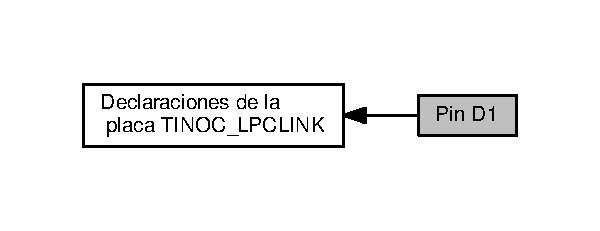
\includegraphics[width=288pt]{group___p_i_n_d1}
\end{center}
\end{figure}
\subsection*{Macros}
\begin{DoxyCompactItemize}
\item 
\#define \hyperlink{group___p_i_n_d1_ga6ae9457c4b1f79250abe5f2960e3a8ee}{L\+P\+C1102\+\_\+\+D1\+\_\+\+B\+IT}~( 1\+U\+L $<$$<$ 7\+U\+L )
\begin{DoxyCompactList}\small\item\em Defino bit del puerto ocupado por D1. \end{DoxyCompactList}\item 
\#define \hyperlink{group___p_i_n_d1_gafc2bbd3830383d98ab56a04c3cd3df20}{L\+P\+C1102\+\_\+\+D1\+\_\+\+P\+O\+RT}~( 1 )
\begin{DoxyCompactList}\small\item\em Defino el port del puerto ocupado por D1. \end{DoxyCompactList}\item 
\#define \hyperlink{group___p_i_n_d1_ga74109f9dcb7ca9657b785faae9d1d142}{L\+P\+C1102\+\_\+\+D1\+\_\+\+G\+P\+IO}~L\+P\+C\+\_\+\+G\+P\+I\+O1
\begin{DoxyCompactList}\small\item\em Defino el registro G\+P\+IO ocupado por D1. \end{DoxyCompactList}\end{DoxyCompactItemize}


\subsection{Detailed Description}


\subsection{Macro Definition Documentation}
\index{Pin D1@{Pin D1}!L\+P\+C1102\+\_\+\+D1\+\_\+\+B\+IT@{L\+P\+C1102\+\_\+\+D1\+\_\+\+B\+IT}}
\index{L\+P\+C1102\+\_\+\+D1\+\_\+\+B\+IT@{L\+P\+C1102\+\_\+\+D1\+\_\+\+B\+IT}!Pin D1@{Pin D1}}
\subsubsection[{\texorpdfstring{L\+P\+C1102\+\_\+\+D1\+\_\+\+B\+IT}{LPC1102_D1_BIT}}]{\setlength{\rightskip}{0pt plus 5cm}\#define L\+P\+C1102\+\_\+\+D1\+\_\+\+B\+IT~( 1\+U\+L $<$$<$ 7\+U\+L )}\hypertarget{group___p_i_n_d1_ga6ae9457c4b1f79250abe5f2960e3a8ee}{}\label{group___p_i_n_d1_ga6ae9457c4b1f79250abe5f2960e3a8ee}


Defino bit del puerto ocupado por D1. 



Definition at line 192 of file tinoc\+\_\+lpclink.\+h.

\index{Pin D1@{Pin D1}!L\+P\+C1102\+\_\+\+D1\+\_\+\+G\+P\+IO@{L\+P\+C1102\+\_\+\+D1\+\_\+\+G\+P\+IO}}
\index{L\+P\+C1102\+\_\+\+D1\+\_\+\+G\+P\+IO@{L\+P\+C1102\+\_\+\+D1\+\_\+\+G\+P\+IO}!Pin D1@{Pin D1}}
\subsubsection[{\texorpdfstring{L\+P\+C1102\+\_\+\+D1\+\_\+\+G\+P\+IO}{LPC1102_D1_GPIO}}]{\setlength{\rightskip}{0pt plus 5cm}\#define L\+P\+C1102\+\_\+\+D1\+\_\+\+G\+P\+IO~L\+P\+C\+\_\+\+G\+P\+I\+O1}\hypertarget{group___p_i_n_d1_ga74109f9dcb7ca9657b785faae9d1d142}{}\label{group___p_i_n_d1_ga74109f9dcb7ca9657b785faae9d1d142}


Defino el registro G\+P\+IO ocupado por D1. 



Definition at line 196 of file tinoc\+\_\+lpclink.\+h.

\index{Pin D1@{Pin D1}!L\+P\+C1102\+\_\+\+D1\+\_\+\+P\+O\+RT@{L\+P\+C1102\+\_\+\+D1\+\_\+\+P\+O\+RT}}
\index{L\+P\+C1102\+\_\+\+D1\+\_\+\+P\+O\+RT@{L\+P\+C1102\+\_\+\+D1\+\_\+\+P\+O\+RT}!Pin D1@{Pin D1}}
\subsubsection[{\texorpdfstring{L\+P\+C1102\+\_\+\+D1\+\_\+\+P\+O\+RT}{LPC1102_D1_PORT}}]{\setlength{\rightskip}{0pt plus 5cm}\#define L\+P\+C1102\+\_\+\+D1\+\_\+\+P\+O\+RT~( 1 )}\hypertarget{group___p_i_n_d1_gafc2bbd3830383d98ab56a04c3cd3df20}{}\label{group___p_i_n_d1_gafc2bbd3830383d98ab56a04c3cd3df20}


Defino el port del puerto ocupado por D1. 



Definition at line 194 of file tinoc\+\_\+lpclink.\+h.


\hypertarget{group___d_e_f_i_n_e_s_l_e_d}{}\section{Definiciones del hardware asociado a los leds.}
\label{group___d_e_f_i_n_e_s_l_e_d}\index{Definiciones del hardware asociado a los leds.@{Definiciones del hardware asociado a los leds.}}


Asociacion de cada L\+ED a pines físicos del M\+CU.  


\subsection*{Macros}
\begin{DoxyCompactItemize}
\item 
\#define \hyperlink{group___d_e_f_i_n_e_s_l_e_d_gaa57bd810e922011351ef20f129cc5411}{L\+E\+D1\+\_\+\+I\+O\+C\+ON}~L\+P\+C\+\_\+\+I\+O\+C\+O\+N\+\_\+\+B4
\begin{DoxyCompactList}\small\item\em Registro I\+O\+C\+ON asociado al L\+E\+D1. \end{DoxyCompactList}\item 
\#define \hyperlink{group___d_e_f_i_n_e_s_l_e_d_ga1787581366e41db5124ae46f50f6dd3b}{L\+E\+D1\+\_\+\+I\+O\+C\+O\+N\+\_\+\+F\+U\+NC}~L\+P\+C\+\_\+\+I\+O\+C\+O\+N\+\_\+\+B4\+\_\+\+F\+U\+N\+C\+\_\+\+P\+I\+O0\+\_\+11
\begin{DoxyCompactList}\small\item\em Función asociada al registro I\+O\+C\+ON. \end{DoxyCompactList}\item 
\#define \hyperlink{group___d_e_f_i_n_e_s_l_e_d_gae2a3615be3480b85cf17a93fdbfb7b7a}{L\+E\+D1\+\_\+\+D\+I\+R\+\_\+\+B\+IT}~( 11\+U\+L )
\begin{DoxyCompactList}\small\item\em Bit asociado al L\+E\+D1. \end{DoxyCompactList}\item 
\#define \hyperlink{group___d_e_f_i_n_e_s_l_e_d_gadac6e35960c534a36409c952d014cb37}{L\+E\+D1\+\_\+\+D\+I\+R\+\_\+\+M\+AS}~( 0x01 $<$$<$ L\+E\+D1\+\_\+\+D\+I\+R\+\_\+\+B\+I\+T )
\begin{DoxyCompactList}\small\item\em Dirección del bit L\+E\+D1. \end{DoxyCompactList}\item 
\#define \hyperlink{group___d_e_f_i_n_e_s_l_e_d_ga365ced0f8a8418c3c8fba173644c7c30}{L\+E\+D1\+\_\+\+D\+I\+R\+\_\+\+R\+EG}~L\+P\+C\+\_\+\+G\+P\+I\+O0-\/$>$D\+IR
\begin{DoxyCompactList}\small\item\em Registro de dirección. \end{DoxyCompactList}\item 
\#define \hyperlink{group___d_e_f_i_n_e_s_l_e_d_ga767d451fb47c4bbbcfbeff51b3d51a7b}{L\+E\+D1\+\_\+\+M\+A\+S\+\_\+\+R\+EG}~L\+P\+C\+\_\+\+G\+P\+I\+O0-\/$>$M\+A\+S\+K\+E\+D\+\_\+\+A\+C\+C\+E\+SS
\begin{DoxyCompactList}\small\item\em Registro I\+O\+C\+ON asociado al L\+E\+D1. \end{DoxyCompactList}\end{DoxyCompactItemize}


\subsection{Detailed Description}
Asociacion de cada L\+ED a pines físicos del M\+CU. 



\subsection{Macro Definition Documentation}
\index{Definiciones del hardware asociado a los leds.@{Definiciones del hardware asociado a los leds.}!L\+E\+D1\+\_\+\+D\+I\+R\+\_\+\+B\+IT@{L\+E\+D1\+\_\+\+D\+I\+R\+\_\+\+B\+IT}}
\index{L\+E\+D1\+\_\+\+D\+I\+R\+\_\+\+B\+IT@{L\+E\+D1\+\_\+\+D\+I\+R\+\_\+\+B\+IT}!Definiciones del hardware asociado a los leds.@{Definiciones del hardware asociado a los leds.}}
\subsubsection[{\texorpdfstring{L\+E\+D1\+\_\+\+D\+I\+R\+\_\+\+B\+IT}{LED1_DIR_BIT}}]{\setlength{\rightskip}{0pt plus 5cm}\#define L\+E\+D1\+\_\+\+D\+I\+R\+\_\+\+B\+IT~( 11\+U\+L )}\hypertarget{group___d_e_f_i_n_e_s_l_e_d_gae2a3615be3480b85cf17a93fdbfb7b7a}{}\label{group___d_e_f_i_n_e_s_l_e_d_gae2a3615be3480b85cf17a93fdbfb7b7a}


Bit asociado al L\+E\+D1. 



Definition at line 37 of file leds.\+h.

\index{Definiciones del hardware asociado a los leds.@{Definiciones del hardware asociado a los leds.}!L\+E\+D1\+\_\+\+D\+I\+R\+\_\+\+M\+AS@{L\+E\+D1\+\_\+\+D\+I\+R\+\_\+\+M\+AS}}
\index{L\+E\+D1\+\_\+\+D\+I\+R\+\_\+\+M\+AS@{L\+E\+D1\+\_\+\+D\+I\+R\+\_\+\+M\+AS}!Definiciones del hardware asociado a los leds.@{Definiciones del hardware asociado a los leds.}}
\subsubsection[{\texorpdfstring{L\+E\+D1\+\_\+\+D\+I\+R\+\_\+\+M\+AS}{LED1_DIR_MAS}}]{\setlength{\rightskip}{0pt plus 5cm}\#define L\+E\+D1\+\_\+\+D\+I\+R\+\_\+\+M\+AS~( 0x01 $<$$<$ L\+E\+D1\+\_\+\+D\+I\+R\+\_\+\+B\+I\+T )}\hypertarget{group___d_e_f_i_n_e_s_l_e_d_gadac6e35960c534a36409c952d014cb37}{}\label{group___d_e_f_i_n_e_s_l_e_d_gadac6e35960c534a36409c952d014cb37}


Dirección del bit L\+E\+D1. 



Definition at line 39 of file leds.\+h.

\index{Definiciones del hardware asociado a los leds.@{Definiciones del hardware asociado a los leds.}!L\+E\+D1\+\_\+\+D\+I\+R\+\_\+\+R\+EG@{L\+E\+D1\+\_\+\+D\+I\+R\+\_\+\+R\+EG}}
\index{L\+E\+D1\+\_\+\+D\+I\+R\+\_\+\+R\+EG@{L\+E\+D1\+\_\+\+D\+I\+R\+\_\+\+R\+EG}!Definiciones del hardware asociado a los leds.@{Definiciones del hardware asociado a los leds.}}
\subsubsection[{\texorpdfstring{L\+E\+D1\+\_\+\+D\+I\+R\+\_\+\+R\+EG}{LED1_DIR_REG}}]{\setlength{\rightskip}{0pt plus 5cm}\#define L\+E\+D1\+\_\+\+D\+I\+R\+\_\+\+R\+EG~L\+P\+C\+\_\+\+G\+P\+I\+O0-\/$>$D\+IR}\hypertarget{group___d_e_f_i_n_e_s_l_e_d_ga365ced0f8a8418c3c8fba173644c7c30}{}\label{group___d_e_f_i_n_e_s_l_e_d_ga365ced0f8a8418c3c8fba173644c7c30}


Registro de dirección. 



Definition at line 41 of file leds.\+h.

\index{Definiciones del hardware asociado a los leds.@{Definiciones del hardware asociado a los leds.}!L\+E\+D1\+\_\+\+I\+O\+C\+ON@{L\+E\+D1\+\_\+\+I\+O\+C\+ON}}
\index{L\+E\+D1\+\_\+\+I\+O\+C\+ON@{L\+E\+D1\+\_\+\+I\+O\+C\+ON}!Definiciones del hardware asociado a los leds.@{Definiciones del hardware asociado a los leds.}}
\subsubsection[{\texorpdfstring{L\+E\+D1\+\_\+\+I\+O\+C\+ON}{LED1_IOCON}}]{\setlength{\rightskip}{0pt plus 5cm}\#define L\+E\+D1\+\_\+\+I\+O\+C\+ON~L\+P\+C\+\_\+\+I\+O\+C\+O\+N\+\_\+\+B4}\hypertarget{group___d_e_f_i_n_e_s_l_e_d_gaa57bd810e922011351ef20f129cc5411}{}\label{group___d_e_f_i_n_e_s_l_e_d_gaa57bd810e922011351ef20f129cc5411}


Registro I\+O\+C\+ON asociado al L\+E\+D1. 



Definition at line 32 of file leds.\+h.

\index{Definiciones del hardware asociado a los leds.@{Definiciones del hardware asociado a los leds.}!L\+E\+D1\+\_\+\+I\+O\+C\+O\+N\+\_\+\+F\+U\+NC@{L\+E\+D1\+\_\+\+I\+O\+C\+O\+N\+\_\+\+F\+U\+NC}}
\index{L\+E\+D1\+\_\+\+I\+O\+C\+O\+N\+\_\+\+F\+U\+NC@{L\+E\+D1\+\_\+\+I\+O\+C\+O\+N\+\_\+\+F\+U\+NC}!Definiciones del hardware asociado a los leds.@{Definiciones del hardware asociado a los leds.}}
\subsubsection[{\texorpdfstring{L\+E\+D1\+\_\+\+I\+O\+C\+O\+N\+\_\+\+F\+U\+NC}{LED1_IOCON_FUNC}}]{\setlength{\rightskip}{0pt plus 5cm}\#define L\+E\+D1\+\_\+\+I\+O\+C\+O\+N\+\_\+\+F\+U\+NC~L\+P\+C\+\_\+\+I\+O\+C\+O\+N\+\_\+\+B4\+\_\+\+F\+U\+N\+C\+\_\+\+P\+I\+O0\+\_\+11}\hypertarget{group___d_e_f_i_n_e_s_l_e_d_ga1787581366e41db5124ae46f50f6dd3b}{}\label{group___d_e_f_i_n_e_s_l_e_d_ga1787581366e41db5124ae46f50f6dd3b}


Función asociada al registro I\+O\+C\+ON. 



Definition at line 34 of file leds.\+h.

\index{Definiciones del hardware asociado a los leds.@{Definiciones del hardware asociado a los leds.}!L\+E\+D1\+\_\+\+M\+A\+S\+\_\+\+R\+EG@{L\+E\+D1\+\_\+\+M\+A\+S\+\_\+\+R\+EG}}
\index{L\+E\+D1\+\_\+\+M\+A\+S\+\_\+\+R\+EG@{L\+E\+D1\+\_\+\+M\+A\+S\+\_\+\+R\+EG}!Definiciones del hardware asociado a los leds.@{Definiciones del hardware asociado a los leds.}}
\subsubsection[{\texorpdfstring{L\+E\+D1\+\_\+\+M\+A\+S\+\_\+\+R\+EG}{LED1_MAS_REG}}]{\setlength{\rightskip}{0pt plus 5cm}\#define L\+E\+D1\+\_\+\+M\+A\+S\+\_\+\+R\+EG~L\+P\+C\+\_\+\+G\+P\+I\+O0-\/$>$M\+A\+S\+K\+E\+D\+\_\+\+A\+C\+C\+E\+SS}\hypertarget{group___d_e_f_i_n_e_s_l_e_d_ga767d451fb47c4bbbcfbeff51b3d51a7b}{}\label{group___d_e_f_i_n_e_s_l_e_d_ga767d451fb47c4bbbcfbeff51b3d51a7b}


Registro I\+O\+C\+ON asociado al L\+E\+D1. 



Definition at line 43 of file leds.\+h.


\hypertarget{group___p_r_i_o_r_i_d_a_d_t_a_r_e_a_s}{}\section{Declaracion de constantes de prioridades}
\label{group___p_r_i_o_r_i_d_a_d_t_a_r_e_a_s}\index{Declaracion de constantes de prioridades@{Declaracion de constantes de prioridades}}


Prioridad asignada a cada tarea.  


\subsection*{Macros}
\begin{DoxyCompactItemize}
\item 
\#define \hyperlink{group___p_r_i_o_r_i_d_a_d_t_a_r_e_a_s_gaeb7652a6bef59d6b2b760ed0258a13b3}{P\+R\+I\+O\+R\+I\+D\+A\+D\+\_\+\+T\+A\+R\+E\+A\+\_\+\+D\+E\+L\+AY}~( \hyperlink{task_8h_a94ed0b9b3b4e8ccc859c322f18583e67}{tsk\+I\+D\+L\+E\+\_\+\+P\+R\+I\+O\+R\+I\+TY} + 2 )
\item 
\#define \hyperlink{group___p_r_i_o_r_i_d_a_d_t_a_r_e_a_s_gad37dbb83921f102e5d414ee65e79c4fe}{P\+R\+I\+O\+R\+I\+D\+A\+D\+\_\+\+T\+A\+R\+E\+A\+\_\+\+P\+A\+R\+P\+A\+D\+E\+AR}~( \hyperlink{task_8h_a94ed0b9b3b4e8ccc859c322f18583e67}{tsk\+I\+D\+L\+E\+\_\+\+P\+R\+I\+O\+R\+I\+TY} + 1 )
\end{DoxyCompactItemize}


\subsection{Detailed Description}
Prioridad asignada a cada tarea. 



\subsection{Macro Definition Documentation}
\index{Declaracion de constantes de prioridades@{Declaracion de constantes de prioridades}!P\+R\+I\+O\+R\+I\+D\+A\+D\+\_\+\+T\+A\+R\+E\+A\+\_\+\+D\+E\+L\+AY@{P\+R\+I\+O\+R\+I\+D\+A\+D\+\_\+\+T\+A\+R\+E\+A\+\_\+\+D\+E\+L\+AY}}
\index{P\+R\+I\+O\+R\+I\+D\+A\+D\+\_\+\+T\+A\+R\+E\+A\+\_\+\+D\+E\+L\+AY@{P\+R\+I\+O\+R\+I\+D\+A\+D\+\_\+\+T\+A\+R\+E\+A\+\_\+\+D\+E\+L\+AY}!Declaracion de constantes de prioridades@{Declaracion de constantes de prioridades}}
\subsubsection[{\texorpdfstring{P\+R\+I\+O\+R\+I\+D\+A\+D\+\_\+\+T\+A\+R\+E\+A\+\_\+\+D\+E\+L\+AY}{PRIORIDAD_TAREA_DELAY}}]{\setlength{\rightskip}{0pt plus 5cm}\#define P\+R\+I\+O\+R\+I\+D\+A\+D\+\_\+\+T\+A\+R\+E\+A\+\_\+\+D\+E\+L\+AY~( {\bf tsk\+I\+D\+L\+E\+\_\+\+P\+R\+I\+O\+R\+I\+TY} + 2 )}\hypertarget{group___p_r_i_o_r_i_d_a_d_t_a_r_e_a_s_gaeb7652a6bef59d6b2b760ed0258a13b3}{}\label{group___p_r_i_o_r_i_d_a_d_t_a_r_e_a_s_gaeb7652a6bef59d6b2b760ed0258a13b3}


Definition at line 56 of file leds.\+h.

\index{Declaracion de constantes de prioridades@{Declaracion de constantes de prioridades}!P\+R\+I\+O\+R\+I\+D\+A\+D\+\_\+\+T\+A\+R\+E\+A\+\_\+\+P\+A\+R\+P\+A\+D\+E\+AR@{P\+R\+I\+O\+R\+I\+D\+A\+D\+\_\+\+T\+A\+R\+E\+A\+\_\+\+P\+A\+R\+P\+A\+D\+E\+AR}}
\index{P\+R\+I\+O\+R\+I\+D\+A\+D\+\_\+\+T\+A\+R\+E\+A\+\_\+\+P\+A\+R\+P\+A\+D\+E\+AR@{P\+R\+I\+O\+R\+I\+D\+A\+D\+\_\+\+T\+A\+R\+E\+A\+\_\+\+P\+A\+R\+P\+A\+D\+E\+AR}!Declaracion de constantes de prioridades@{Declaracion de constantes de prioridades}}
\subsubsection[{\texorpdfstring{P\+R\+I\+O\+R\+I\+D\+A\+D\+\_\+\+T\+A\+R\+E\+A\+\_\+\+P\+A\+R\+P\+A\+D\+E\+AR}{PRIORIDAD_TAREA_PARPADEAR}}]{\setlength{\rightskip}{0pt plus 5cm}\#define P\+R\+I\+O\+R\+I\+D\+A\+D\+\_\+\+T\+A\+R\+E\+A\+\_\+\+P\+A\+R\+P\+A\+D\+E\+AR~( {\bf tsk\+I\+D\+L\+E\+\_\+\+P\+R\+I\+O\+R\+I\+TY} + 1 )}\hypertarget{group___p_r_i_o_r_i_d_a_d_t_a_r_e_a_s_gad37dbb83921f102e5d414ee65e79c4fe}{}\label{group___p_r_i_o_r_i_d_a_d_t_a_r_e_a_s_gad37dbb83921f102e5d414ee65e79c4fe}


Definition at line 58 of file leds.\+h.


\hypertarget{group___h_o_o_k_f_u_n_c_t_i_o_n_s}{}\section{Funciones \char`\"{}\+Hook\char`\"{} del Free\+R\+T\+OS}
\label{group___h_o_o_k_f_u_n_c_t_i_o_n_s}\index{Funciones \char`\"{}\+Hook\char`\"{} del Free\+R\+T\+OS@{Funciones ""Hook"" del Free\+R\+T\+OS}}


Funciones handler de eventos de excepcion.  


\subsection*{Functions}
\begin{DoxyCompactItemize}
\item 
void \hyperlink{group___h_o_o_k_f_u_n_c_t_i_o_n_s_gab7e5c95cf72a3f819bc4462a7fb62ca3}{v\+Application\+Malloc\+Failed\+Hook} (void)
\begin{DoxyCompactList}\small\item\em \hyperlink{group___h_o_o_k_f_u_n_c_t_i_o_n_s_gab7e5c95cf72a3f819bc4462a7fb62ca3}{v\+Application\+Malloc\+Failed\+Hook()} will only be called if \end{DoxyCompactList}\item 
void \hyperlink{group___h_o_o_k_f_u_n_c_t_i_o_n_s_ga97fd430f36f8b065226e2bff9bad1de5}{v\+Application\+Idle\+Hook} (void)
\begin{DoxyCompactList}\small\item\em \hyperlink{group___h_o_o_k_f_u_n_c_t_i_o_n_s_ga97fd430f36f8b065226e2bff9bad1de5}{v\+Application\+Idle\+Hook()} will only be called if config\+U\+S\+E\+\_\+\+I\+D\+L\+E\+\_\+\+H\+O\+OK is set \end{DoxyCompactList}\item 
void \hyperlink{group___h_o_o_k_f_u_n_c_t_i_o_n_s_ga306672a74bdd13ce210c05fca3385c59}{v\+Application\+Stack\+Overflow\+Hook} (\hyperlink{task_8h_ae95f44d4cfeb4a599c6cc258d241cb6b}{Task\+Handle\+\_\+t} px\+Task, char $\ast$pc\+Task\+Name)
\begin{DoxyCompactList}\small\item\em Run time stack overflow checking is performed if. \end{DoxyCompactList}\item 
void \hyperlink{group___h_o_o_k_f_u_n_c_t_i_o_n_s_ga9ca051aa77e17583aa5a85d5de5c199a}{v\+Application\+Tick\+Hook} (void)
\begin{DoxyCompactList}\small\item\em This function will be called by each tick interrupt if config\+U\+S\+E\+\_\+\+T\+I\+C\+K\+\_\+\+H\+O\+OK is set to 1 in \hyperlink{_free_r_t_o_s_config_8h}{Free\+R\+T\+O\+S\+Config.\+h}. User code can be added here, but the tick hook is called from an interrupt context, so code must not attempt to block, and only the interrupt safe Free\+R\+T\+OS A\+PI functions can be used (those that end in From\+I\+S\+R()). Manually check the last few bytes of the interrupt stack to check they have not been overwritten. Note -\/ the task stacks are automatically checked for overflow if config\+C\+H\+E\+C\+K\+\_\+\+F\+O\+R\+\_\+\+S\+T\+A\+C\+K\+\_\+\+O\+V\+E\+R\+F\+L\+OW is set to 1 or 2 in Free\+R\+T\+O\+S\+Conifg.\+h, but the interrupt stack is not. \end{DoxyCompactList}\end{DoxyCompactItemize}


\subsection{Detailed Description}
Funciones handler de eventos de excepcion. 



\subsection{Function Documentation}
\index{Funciones \char`\"{}\+Hook\char`\"{} del Free\+R\+T\+OS@{Funciones ""Hook"" del Free\+R\+T\+OS}!v\+Application\+Idle\+Hook@{v\+Application\+Idle\+Hook}}
\index{v\+Application\+Idle\+Hook@{v\+Application\+Idle\+Hook}!Funciones \char`\"{}\+Hook\char`\"{} del Free\+R\+T\+OS@{Funciones ""Hook"" del Free\+R\+T\+OS}}
\subsubsection[{\texorpdfstring{v\+Application\+Idle\+Hook(void)}{vApplicationIdleHook(void)}}]{\setlength{\rightskip}{0pt plus 5cm}void v\+Application\+Idle\+Hook (
\begin{DoxyParamCaption}
\item[{void}]{}
\end{DoxyParamCaption}
)}\hypertarget{group___h_o_o_k_f_u_n_c_t_i_o_n_s_ga97fd430f36f8b065226e2bff9bad1de5}{}\label{group___h_o_o_k_f_u_n_c_t_i_o_n_s_ga97fd430f36f8b065226e2bff9bad1de5}


\hyperlink{group___h_o_o_k_f_u_n_c_t_i_o_n_s_ga97fd430f36f8b065226e2bff9bad1de5}{v\+Application\+Idle\+Hook()} will only be called if config\+U\+S\+E\+\_\+\+I\+D\+L\+E\+\_\+\+H\+O\+OK is set 

void \hyperlink{group___h_o_o_k_f_u_n_c_t_i_o_n_s_ga97fd430f36f8b065226e2bff9bad1de5}{v\+Application\+Idle\+Hook( void )} to 1 in \hyperlink{_free_r_t_o_s_config_8h}{Free\+R\+T\+O\+S\+Config.\+h}. It will be called on each iteration of the idle task. It is essential that code added to this hook function never attempts to block in any way (for example, call \hyperlink{queue_8h_af1549eac0e7f05694a59a0b967c80be3}{x\+Queue\+Receive()} with a block time specified, or call \hyperlink{task_8h_aa154068cecd7f31446a7a84af44ab1a3}{v\+Task\+Delay()}). If the application makes use of the \hyperlink{task_8h_a27ff4ebce26565bef136bda84201ff80}{v\+Task\+Delete()} A\+PI function (as this demo application does) then it is also important that \hyperlink{group___h_o_o_k_f_u_n_c_t_i_o_n_s_ga97fd430f36f8b065226e2bff9bad1de5}{v\+Application\+Idle\+Hook()} is permitted to return to its calling function, because it is the responsibility of the idle task to clean up memory allocated by the kernel to any task that has since been deleted. \begin{DoxyAuthor}{Author}
N\+XP 
\end{DoxyAuthor}


Definition at line 306 of file main.\+c.

\index{Funciones \char`\"{}\+Hook\char`\"{} del Free\+R\+T\+OS@{Funciones ""Hook"" del Free\+R\+T\+OS}!v\+Application\+Malloc\+Failed\+Hook@{v\+Application\+Malloc\+Failed\+Hook}}
\index{v\+Application\+Malloc\+Failed\+Hook@{v\+Application\+Malloc\+Failed\+Hook}!Funciones \char`\"{}\+Hook\char`\"{} del Free\+R\+T\+OS@{Funciones ""Hook"" del Free\+R\+T\+OS}}
\subsubsection[{\texorpdfstring{v\+Application\+Malloc\+Failed\+Hook(void)}{vApplicationMallocFailedHook(void)}}]{\setlength{\rightskip}{0pt plus 5cm}void v\+Application\+Malloc\+Failed\+Hook (
\begin{DoxyParamCaption}
\item[{void}]{}
\end{DoxyParamCaption}
)}\hypertarget{group___h_o_o_k_f_u_n_c_t_i_o_n_s_gab7e5c95cf72a3f819bc4462a7fb62ca3}{}\label{group___h_o_o_k_f_u_n_c_t_i_o_n_s_gab7e5c95cf72a3f819bc4462a7fb62ca3}


\hyperlink{group___h_o_o_k_f_u_n_c_t_i_o_n_s_gab7e5c95cf72a3f819bc4462a7fb62ca3}{v\+Application\+Malloc\+Failed\+Hook()} will only be called if 

void \hyperlink{group___h_o_o_k_f_u_n_c_t_i_o_n_s_gab7e5c95cf72a3f819bc4462a7fb62ca3}{v\+Application\+Malloc\+Failed\+Hook( void )} config\+U\+S\+E\+\_\+\+M\+A\+L\+L\+O\+C\+\_\+\+F\+A\+I\+L\+E\+D\+\_\+\+H\+O\+OK is set to 1 in \hyperlink{_free_r_t_o_s_config_8h}{Free\+R\+T\+O\+S\+Config.\+h}. It is a hook function that will get called if a call to \hyperlink{portable_8h_a237d63f90b28e0950bd86f76815cd6e3}{pv\+Port\+Malloc()} fails. \hyperlink{portable_8h_a237d63f90b28e0950bd86f76815cd6e3}{pv\+Port\+Malloc()} is called internally by the kernel whenever a task, queue, timer or semaphore is created. It is also called by various parts of the demo application. If \hyperlink{heap__1_8c}{heap\+\_\+1.\+c} or heap\+\_\+2.\+c are used, then the size of the heap available to \hyperlink{portable_8h_a237d63f90b28e0950bd86f76815cd6e3}{pv\+Port\+Malloc()} is defined by config\+T\+O\+T\+A\+L\+\_\+\+H\+E\+A\+P\+\_\+\+S\+I\+ZE in \hyperlink{_free_r_t_o_s_config_8h}{Free\+R\+T\+O\+S\+Config.\+h}, and the \hyperlink{portable_8h_a8f72fbee5c25c956bda528299ce6dd02}{x\+Port\+Get\+Free\+Heap\+Size()} A\+PI function can be used to query the size of free heap space that remains (although it does not provide information on how the remaining heap might be fragmented). memory, etc. are configured before \hyperlink{main_8c_a840291bc02cba5474a4cb46a9b9566fe}{main()} is called. \begin{DoxyAuthor}{Author}
N\+XP 
\end{DoxyAuthor}


Definition at line 284 of file main.\+c.

\index{Funciones \char`\"{}\+Hook\char`\"{} del Free\+R\+T\+OS@{Funciones ""Hook"" del Free\+R\+T\+OS}!v\+Application\+Stack\+Overflow\+Hook@{v\+Application\+Stack\+Overflow\+Hook}}
\index{v\+Application\+Stack\+Overflow\+Hook@{v\+Application\+Stack\+Overflow\+Hook}!Funciones \char`\"{}\+Hook\char`\"{} del Free\+R\+T\+OS@{Funciones ""Hook"" del Free\+R\+T\+OS}}
\subsubsection[{\texorpdfstring{v\+Application\+Stack\+Overflow\+Hook(\+Task\+Handle\+\_\+t px\+Task, char $\ast$pc\+Task\+Name)}{vApplicationStackOverflowHook(TaskHandle_t pxTask, char *pcTaskName)}}]{\setlength{\rightskip}{0pt plus 5cm}void v\+Application\+Stack\+Overflow\+Hook (
\begin{DoxyParamCaption}
\item[{{\bf Task\+Handle\+\_\+t}}]{px\+Task, }
\item[{char $\ast$}]{pc\+Task\+Name}
\end{DoxyParamCaption}
)}\hypertarget{group___h_o_o_k_f_u_n_c_t_i_o_n_s_ga306672a74bdd13ce210c05fca3385c59}{}\label{group___h_o_o_k_f_u_n_c_t_i_o_n_s_ga306672a74bdd13ce210c05fca3385c59}


Run time stack overflow checking is performed if. 

void \hyperlink{group___h_o_o_k_f_u_n_c_t_i_o_n_s_ga306672a74bdd13ce210c05fca3385c59}{v\+Application\+Stack\+Overflow\+Hook( Task\+Handle\+\_\+t px\+Task, char $\ast$pc\+Task\+Name )} config\+C\+H\+E\+C\+K\+\_\+\+F\+O\+R\+\_\+\+S\+T\+A\+C\+K\+\_\+\+O\+V\+E\+R\+F\+L\+OW is defined to 1 or 2. This hook function is called if a stack overflow is detected. \begin{DoxyAuthor}{Author}
N\+XP 
\end{DoxyAuthor}


Definition at line 321 of file main.\+c.

\index{Funciones \char`\"{}\+Hook\char`\"{} del Free\+R\+T\+OS@{Funciones ""Hook"" del Free\+R\+T\+OS}!v\+Application\+Tick\+Hook@{v\+Application\+Tick\+Hook}}
\index{v\+Application\+Tick\+Hook@{v\+Application\+Tick\+Hook}!Funciones \char`\"{}\+Hook\char`\"{} del Free\+R\+T\+OS@{Funciones ""Hook"" del Free\+R\+T\+OS}}
\subsubsection[{\texorpdfstring{v\+Application\+Tick\+Hook(void)}{vApplicationTickHook(void)}}]{\setlength{\rightskip}{0pt plus 5cm}void v\+Application\+Tick\+Hook (
\begin{DoxyParamCaption}
\item[{void}]{}
\end{DoxyParamCaption}
)}\hypertarget{group___h_o_o_k_f_u_n_c_t_i_o_n_s_ga9ca051aa77e17583aa5a85d5de5c199a}{}\label{group___h_o_o_k_f_u_n_c_t_i_o_n_s_ga9ca051aa77e17583aa5a85d5de5c199a}


This function will be called by each tick interrupt if config\+U\+S\+E\+\_\+\+T\+I\+C\+K\+\_\+\+H\+O\+OK is set to 1 in \hyperlink{_free_r_t_o_s_config_8h}{Free\+R\+T\+O\+S\+Config.\+h}. User code can be added here, but the tick hook is called from an interrupt context, so code must not attempt to block, and only the interrupt safe Free\+R\+T\+OS A\+PI functions can be used (those that end in From\+I\+S\+R()). Manually check the last few bytes of the interrupt stack to check they have not been overwritten. Note -\/ the task stacks are automatically checked for overflow if config\+C\+H\+E\+C\+K\+\_\+\+F\+O\+R\+\_\+\+S\+T\+A\+C\+K\+\_\+\+O\+V\+E\+R\+F\+L\+OW is set to 1 or 2 in Free\+R\+T\+O\+S\+Conifg.\+h, but the interrupt stack is not. 

v\+Application\+Tick\+Hook

\begin{DoxyAuthor}{Author}
N\+XP 
\end{DoxyAuthor}


Definition at line 351 of file main.\+c.


\hypertarget{group___d_e_f_i_n_e_s_u_a_r_t}{}\section{Definiciones asociadas al manejo de la U\+A\+RT}
\label{group___d_e_f_i_n_e_s_u_a_r_t}\index{Definiciones asociadas al manejo de la U\+A\+RT@{Definiciones asociadas al manejo de la U\+A\+RT}}


Definiciones de constantes de registros y funciones de la U\+A\+RT.  


Collaboration diagram for Definiciones asociadas al manejo de la U\+A\+RT\+:\nopagebreak
\begin{figure}[H]
\begin{center}
\leavevmode
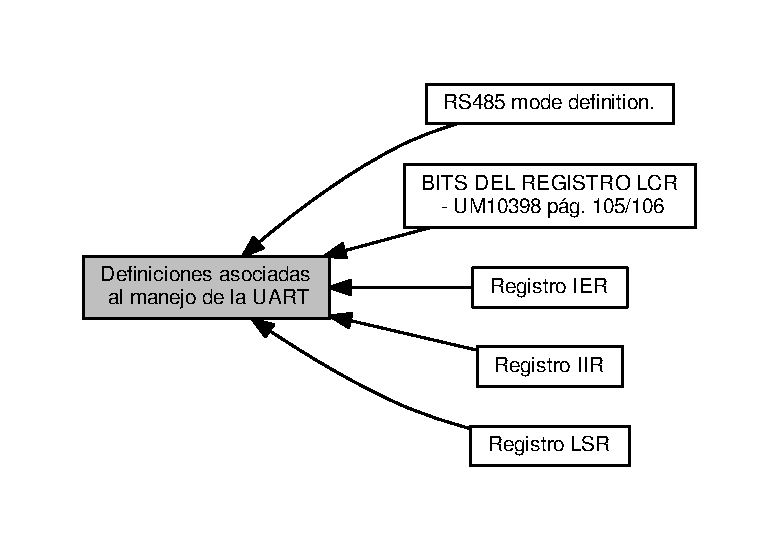
\includegraphics[width=350pt]{group___d_e_f_i_n_e_s_u_a_r_t}
\end{center}
\end{figure}
\subsection*{Modules}
\begin{DoxyCompactItemize}
\item 
\hyperlink{group___r_e_g_i_s_t_r_o___i_e_r}{Registro I\+ER}
\begin{DoxyCompactList}\small\item\em Definiciones asociadas al registro Interrupt Enable Register (U0\+I\+ER)~\newline
 Descripciones copiada directamente del manual U\+M10398 pag. 202. \end{DoxyCompactList}\item 
\hyperlink{group___r_e_g_i_s_t_r_o___i_i_r}{Registro I\+IR}
\begin{DoxyCompactList}\small\item\em Definiciones asociadas al registro Interrupt Enable Register (U0\+I\+ER)~\newline
 Descripciones copiada directamente del manual U\+M10398 pag. 203. \end{DoxyCompactList}\item 
\hyperlink{group___r_e_g_i_s_t_r_o___l_s_r}{Registro L\+SR}
\begin{DoxyCompactList}\small\item\em Definiciones asociadas al registro Line Status Register (U0\+L\+SR)~\newline
 Descripciones copiada directamente del manual U\+M10398 pag. 210~\newline
 The U0\+L\+SR is a Read Only register that provides status information on the U\+A\+RT TX and RX blocks.~\newline
. \end{DoxyCompactList}\item 
\hyperlink{group___r_s485_m_o_d_e}{R\+S485 mode definition.}
\begin{DoxyCompactList}\small\item\em The U0\+R\+S485\+C\+T\+RL register controls the configuration of the U\+A\+RT in R\+S-\/485/\+E\+I\+A-\/485 mode. \end{DoxyCompactList}\item 
\hyperlink{group___l_c_r_b_i_t_s}{B\+I\+T\+S D\+E\+L R\+E\+G\+I\+S\+T\+R\+O L\+C\+R -\/ U\+M10398 pág. 105/106}
\begin{DoxyCompactList}\small\item\em The U0\+L\+CR determines the format of the data character that is to be transmitted or received. \end{DoxyCompactList}\end{DoxyCompactItemize}
\subsection*{Macros}
\begin{DoxyCompactItemize}
\item 
\#define \hyperlink{group___d_e_f_i_n_e_s_u_a_r_t_ga8557658113e8a497db405dac37ca0c71}{T\+X\+\_\+\+I\+N\+T\+E\+R\+R\+U\+PT}~1
\begin{DoxyCompactList}\small\item\em 0 if TX uses polling, 1 interrupt driven. \end{DoxyCompactList}\item 
\#define \hyperlink{group___d_e_f_i_n_e_s_u_a_r_t_gaeca034f67218340ecb2261a22c2f3dcd}{B\+U\+F\+S\+I\+ZE}~0x40
\begin{DoxyCompactList}\small\item\em Tamaño del buffer de almacenamiento intermedio. \end{DoxyCompactList}\item 
\#define \hyperlink{group___d_e_f_i_n_e_s_u_a_r_t_ga3ba6411298b98763494970e394042bed}{B\+A\+U\+D\+\_\+\+R\+A\+T\+E\+\_\+\+D\+E\+F\+A\+U\+LT}~9600
\begin{DoxyCompactList}\small\item\em D\+E\+F\+I\+N\+I\+C\+I\+O\+N\+ES P\+OR D\+E\+F\+A\+U\+LT. \end{DoxyCompactList}\item 
\#define \hyperlink{group___d_e_f_i_n_e_s_u_a_r_t_gad4455691936f92fdd6c37566fc58ba1f}{B\+A\+U\+D\+\_\+\+R\+A\+TE}~\hyperlink{group___d_e_f_i_n_e_s_u_a_r_t_ga3ba6411298b98763494970e394042bed}{B\+A\+U\+D\+\_\+\+R\+A\+T\+E\+\_\+\+D\+E\+F\+A\+U\+LT}
\begin{DoxyCompactList}\small\item\em Velocidad de transmisión U\+A\+RT. \end{DoxyCompactList}\item 
\#define \hyperlink{group___d_e_f_i_n_e_s_u_a_r_t_ga15fcd73e7add5fb7be07914dcf174eda}{\+\_\+\+R\+S485\+\_\+\+U\+S\+A\+R\+\_\+\+R\+T\+S\+\_\+\+D\+IR}
\item 
\#define \hyperlink{group___d_e_f_i_n_e_s_u_a_r_t_ga7d503384123e41cba57ad7b306df19d8}{R\+T\+S\+\_\+\+P\+O\+RT}~1
\begin{DoxyCompactList}\small\item\em P1.\+5/neg(R\+TS)/\+C\+T32\+B0\+\_\+\+C\+A\+P0 U\+M10398 pág. 79. \end{DoxyCompactList}\item 
\#define \hyperlink{group___d_e_f_i_n_e_s_u_a_r_t_ga4a2c9474c826c040eb2f4d36fdf98509}{R\+T\+S\+\_\+\+P\+IN}~5
\begin{DoxyCompactList}\small\item\em P1.\+5/neg(R\+TS)/\+C\+T32\+B0\+\_\+\+C\+A\+P0 U\+M10398 pág. 79. \end{DoxyCompactList}\item 
\#define \hyperlink{group___d_e_f_i_n_e_s_u_a_r_t_gac83cc62ddf027024055e8b2ddbfb14d8}{R\+S485\+\_\+\+D\+I\+R\+\_\+\+P\+O\+RT}~\hyperlink{group___d_e_f_i_n_e_s_u_a_r_t_ga7d503384123e41cba57ad7b306df19d8}{R\+T\+S\+\_\+\+P\+O\+RT}
\begin{DoxyCompactList}\small\item\em puerto utilizado para manejo de dirección del puerto R\+S485 \end{DoxyCompactList}\item 
\#define \hyperlink{group___d_e_f_i_n_e_s_u_a_r_t_ga0c3dd11efc19d493e0776ae590a342fd}{R\+S485\+\_\+\+D\+I\+R\+\_\+\+P\+IN}~\hyperlink{group___d_e_f_i_n_e_s_u_a_r_t_ga4a2c9474c826c040eb2f4d36fdf98509}{R\+T\+S\+\_\+\+P\+IN}
\begin{DoxyCompactList}\small\item\em pin utilizado para manejo de dirección del puerto R\+S485 \end{DoxyCompactList}\item 
\#define \hyperlink{group___d_e_f_i_n_e_s_u_a_r_t_ga6a815f4456be0ae15fd74ff2172d2d4e}{R\+S485\+\_\+\+D\+E\+F\+I\+N\+I\+R\+\_\+\+P\+IN}()~\hyperlink{gpio_8h_a376642dd36001cc5eb409f9c83152e60}{G\+P\+I\+O\+Set\+Dir}( \hyperlink{group___d_e_f_i_n_e_s_u_a_r_t_gac83cc62ddf027024055e8b2ddbfb14d8}{R\+S485\+\_\+\+D\+I\+R\+\_\+\+P\+O\+RT}, \hyperlink{group___d_e_f_i_n_e_s_u_a_r_t_ga0c3dd11efc19d493e0776ae590a342fd}{R\+S485\+\_\+\+D\+I\+R\+\_\+\+P\+IN}, 1 )
\begin{DoxyCompactList}\small\item\em Inicializo pin de salida para direccionar R\+S485. \end{DoxyCompactList}\item 
\#define \hyperlink{group___d_e_f_i_n_e_s_u_a_r_t_gad21e8ee2f3bf01827e41e73325765c8a}{R\+S485\+\_\+\+H\+A\+B\+I\+L\+I\+T\+A\+R\+\_\+\+TX}()~\hyperlink{gpio_8h_a6e2440fb6429a69f1338b51a4cab2921}{G\+P\+I\+O\+Set\+Value}(\hyperlink{group___d_e_f_i_n_e_s_u_a_r_t_gac83cc62ddf027024055e8b2ddbfb14d8}{R\+S485\+\_\+\+D\+I\+R\+\_\+\+P\+O\+RT}, \hyperlink{group___d_e_f_i_n_e_s_u_a_r_t_ga0c3dd11efc19d493e0776ae590a342fd}{R\+S485\+\_\+\+D\+I\+R\+\_\+\+P\+IN}, 1)
\begin{DoxyCompactList}\small\item\em Seteo el pin en bajo para habilitar la recepción. \end{DoxyCompactList}\item 
\#define \hyperlink{group___d_e_f_i_n_e_s_u_a_r_t_ga32978f6a50d8f84d883b95c39df21da2}{R\+S485\+\_\+\+H\+A\+B\+I\+L\+I\+T\+A\+R\+\_\+\+RX}()~\hyperlink{gpio_8h_a6e2440fb6429a69f1338b51a4cab2921}{G\+P\+I\+O\+Set\+Value}(\hyperlink{group___d_e_f_i_n_e_s_u_a_r_t_gac83cc62ddf027024055e8b2ddbfb14d8}{R\+S485\+\_\+\+D\+I\+R\+\_\+\+P\+O\+RT}, \hyperlink{group___d_e_f_i_n_e_s_u_a_r_t_ga0c3dd11efc19d493e0776ae590a342fd}{R\+S485\+\_\+\+D\+I\+R\+\_\+\+P\+IN}, 0)
\begin{DoxyCompactList}\small\item\em Seteo el pin en bajo para habilitar la recepción. \end{DoxyCompactList}\item 
\#define \hyperlink{group___d_e_f_i_n_e_s_u_a_r_t_gad3c62ebbc4b69ec10a8e68be7f85fb1e}{receive\+Q\+U\+E\+U\+E\+\_\+\+L\+E\+N\+G\+TH}~( 10 )
\end{DoxyCompactItemize}


\subsection{Detailed Description}
Definiciones de constantes de registros y funciones de la U\+A\+RT. 

\begin{DoxyAuthor}{Author}
Ing. Roux, Federico G. (\href{mailto:froux@citedef.gob.ar}{\tt froux@citedef.\+gob.\+ar}) 
\end{DoxyAuthor}


\subsection{Macro Definition Documentation}
\index{Definiciones asociadas al manejo de la U\+A\+RT@{Definiciones asociadas al manejo de la U\+A\+RT}!\+\_\+\+R\+S485\+\_\+\+U\+S\+A\+R\+\_\+\+R\+T\+S\+\_\+\+D\+IR@{\+\_\+\+R\+S485\+\_\+\+U\+S\+A\+R\+\_\+\+R\+T\+S\+\_\+\+D\+IR}}
\index{\+\_\+\+R\+S485\+\_\+\+U\+S\+A\+R\+\_\+\+R\+T\+S\+\_\+\+D\+IR@{\+\_\+\+R\+S485\+\_\+\+U\+S\+A\+R\+\_\+\+R\+T\+S\+\_\+\+D\+IR}!Definiciones asociadas al manejo de la U\+A\+RT@{Definiciones asociadas al manejo de la U\+A\+RT}}
\subsubsection[{\texorpdfstring{\+\_\+\+R\+S485\+\_\+\+U\+S\+A\+R\+\_\+\+R\+T\+S\+\_\+\+D\+IR}{_RS485_USAR_RTS_DIR}}]{\setlength{\rightskip}{0pt plus 5cm}\#define \+\_\+\+R\+S485\+\_\+\+U\+S\+A\+R\+\_\+\+R\+T\+S\+\_\+\+D\+IR}\hypertarget{group___d_e_f_i_n_e_s_u_a_r_t_ga15fcd73e7add5fb7be07914dcf174eda}{}\label{group___d_e_f_i_n_e_s_u_a_r_t_ga15fcd73e7add5fb7be07914dcf174eda}


Definition at line 352 of file uart.\+h.

\index{Definiciones asociadas al manejo de la U\+A\+RT@{Definiciones asociadas al manejo de la U\+A\+RT}!B\+A\+U\+D\+\_\+\+R\+A\+TE@{B\+A\+U\+D\+\_\+\+R\+A\+TE}}
\index{B\+A\+U\+D\+\_\+\+R\+A\+TE@{B\+A\+U\+D\+\_\+\+R\+A\+TE}!Definiciones asociadas al manejo de la U\+A\+RT@{Definiciones asociadas al manejo de la U\+A\+RT}}
\subsubsection[{\texorpdfstring{B\+A\+U\+D\+\_\+\+R\+A\+TE}{BAUD_RATE}}]{\setlength{\rightskip}{0pt plus 5cm}\#define B\+A\+U\+D\+\_\+\+R\+A\+TE~{\bf B\+A\+U\+D\+\_\+\+R\+A\+T\+E\+\_\+\+D\+E\+F\+A\+U\+LT}}\hypertarget{group___d_e_f_i_n_e_s_u_a_r_t_gad4455691936f92fdd6c37566fc58ba1f}{}\label{group___d_e_f_i_n_e_s_u_a_r_t_gad4455691936f92fdd6c37566fc58ba1f}


Velocidad de transmisión U\+A\+RT. 



Definition at line 348 of file uart.\+h.

\index{Definiciones asociadas al manejo de la U\+A\+RT@{Definiciones asociadas al manejo de la U\+A\+RT}!B\+A\+U\+D\+\_\+\+R\+A\+T\+E\+\_\+\+D\+E\+F\+A\+U\+LT@{B\+A\+U\+D\+\_\+\+R\+A\+T\+E\+\_\+\+D\+E\+F\+A\+U\+LT}}
\index{B\+A\+U\+D\+\_\+\+R\+A\+T\+E\+\_\+\+D\+E\+F\+A\+U\+LT@{B\+A\+U\+D\+\_\+\+R\+A\+T\+E\+\_\+\+D\+E\+F\+A\+U\+LT}!Definiciones asociadas al manejo de la U\+A\+RT@{Definiciones asociadas al manejo de la U\+A\+RT}}
\subsubsection[{\texorpdfstring{B\+A\+U\+D\+\_\+\+R\+A\+T\+E\+\_\+\+D\+E\+F\+A\+U\+LT}{BAUD_RATE_DEFAULT}}]{\setlength{\rightskip}{0pt plus 5cm}\#define B\+A\+U\+D\+\_\+\+R\+A\+T\+E\+\_\+\+D\+E\+F\+A\+U\+LT~9600}\hypertarget{group___d_e_f_i_n_e_s_u_a_r_t_ga3ba6411298b98763494970e394042bed}{}\label{group___d_e_f_i_n_e_s_u_a_r_t_ga3ba6411298b98763494970e394042bed}


D\+E\+F\+I\+N\+I\+C\+I\+O\+N\+ES P\+OR D\+E\+F\+A\+U\+LT. 



Definition at line 344 of file uart.\+h.

\index{Definiciones asociadas al manejo de la U\+A\+RT@{Definiciones asociadas al manejo de la U\+A\+RT}!B\+U\+F\+S\+I\+ZE@{B\+U\+F\+S\+I\+ZE}}
\index{B\+U\+F\+S\+I\+ZE@{B\+U\+F\+S\+I\+ZE}!Definiciones asociadas al manejo de la U\+A\+RT@{Definiciones asociadas al manejo de la U\+A\+RT}}
\subsubsection[{\texorpdfstring{B\+U\+F\+S\+I\+ZE}{BUFSIZE}}]{\setlength{\rightskip}{0pt plus 5cm}\#define B\+U\+F\+S\+I\+ZE~0x40}\hypertarget{group___d_e_f_i_n_e_s_u_a_r_t_gaeca034f67218340ecb2261a22c2f3dcd}{}\label{group___d_e_f_i_n_e_s_u_a_r_t_gaeca034f67218340ecb2261a22c2f3dcd}


Tamaño del buffer de almacenamiento intermedio. 



Definition at line 244 of file uart.\+h.

\index{Definiciones asociadas al manejo de la U\+A\+RT@{Definiciones asociadas al manejo de la U\+A\+RT}!receive\+Q\+U\+E\+U\+E\+\_\+\+L\+E\+N\+G\+TH@{receive\+Q\+U\+E\+U\+E\+\_\+\+L\+E\+N\+G\+TH}}
\index{receive\+Q\+U\+E\+U\+E\+\_\+\+L\+E\+N\+G\+TH@{receive\+Q\+U\+E\+U\+E\+\_\+\+L\+E\+N\+G\+TH}!Definiciones asociadas al manejo de la U\+A\+RT@{Definiciones asociadas al manejo de la U\+A\+RT}}
\subsubsection[{\texorpdfstring{receive\+Q\+U\+E\+U\+E\+\_\+\+L\+E\+N\+G\+TH}{receiveQUEUE_LENGTH}}]{\setlength{\rightskip}{0pt plus 5cm}\#define receive\+Q\+U\+E\+U\+E\+\_\+\+L\+E\+N\+G\+TH~( 10 )}\hypertarget{group___d_e_f_i_n_e_s_u_a_r_t_gad3c62ebbc4b69ec10a8e68be7f85fb1e}{}\label{group___d_e_f_i_n_e_s_u_a_r_t_gad3c62ebbc4b69ec10a8e68be7f85fb1e}


Definition at line 380 of file uart.\+h.

\index{Definiciones asociadas al manejo de la U\+A\+RT@{Definiciones asociadas al manejo de la U\+A\+RT}!R\+S485\+\_\+\+D\+E\+F\+I\+N\+I\+R\+\_\+\+P\+IN@{R\+S485\+\_\+\+D\+E\+F\+I\+N\+I\+R\+\_\+\+P\+IN}}
\index{R\+S485\+\_\+\+D\+E\+F\+I\+N\+I\+R\+\_\+\+P\+IN@{R\+S485\+\_\+\+D\+E\+F\+I\+N\+I\+R\+\_\+\+P\+IN}!Definiciones asociadas al manejo de la U\+A\+RT@{Definiciones asociadas al manejo de la U\+A\+RT}}
\subsubsection[{\texorpdfstring{R\+S485\+\_\+\+D\+E\+F\+I\+N\+I\+R\+\_\+\+P\+IN}{RS485_DEFINIR_PIN}}]{\setlength{\rightskip}{0pt plus 5cm}\#define R\+S485\+\_\+\+D\+E\+F\+I\+N\+I\+R\+\_\+\+P\+IN(
\begin{DoxyParamCaption}
{}
\end{DoxyParamCaption}
)~{\bf G\+P\+I\+O\+Set\+Dir}( {\bf R\+S485\+\_\+\+D\+I\+R\+\_\+\+P\+O\+RT}, {\bf R\+S485\+\_\+\+D\+I\+R\+\_\+\+P\+IN}, 1 )}\hypertarget{group___d_e_f_i_n_e_s_u_a_r_t_ga6a815f4456be0ae15fd74ff2172d2d4e}{}\label{group___d_e_f_i_n_e_s_u_a_r_t_ga6a815f4456be0ae15fd74ff2172d2d4e}


Inicializo pin de salida para direccionar R\+S485. 



Definition at line 374 of file uart.\+h.

\index{Definiciones asociadas al manejo de la U\+A\+RT@{Definiciones asociadas al manejo de la U\+A\+RT}!R\+S485\+\_\+\+D\+I\+R\+\_\+\+P\+IN@{R\+S485\+\_\+\+D\+I\+R\+\_\+\+P\+IN}}
\index{R\+S485\+\_\+\+D\+I\+R\+\_\+\+P\+IN@{R\+S485\+\_\+\+D\+I\+R\+\_\+\+P\+IN}!Definiciones asociadas al manejo de la U\+A\+RT@{Definiciones asociadas al manejo de la U\+A\+RT}}
\subsubsection[{\texorpdfstring{R\+S485\+\_\+\+D\+I\+R\+\_\+\+P\+IN}{RS485_DIR_PIN}}]{\setlength{\rightskip}{0pt plus 5cm}\#define R\+S485\+\_\+\+D\+I\+R\+\_\+\+P\+IN~{\bf R\+T\+S\+\_\+\+P\+IN}}\hypertarget{group___d_e_f_i_n_e_s_u_a_r_t_ga0c3dd11efc19d493e0776ae590a342fd}{}\label{group___d_e_f_i_n_e_s_u_a_r_t_ga0c3dd11efc19d493e0776ae590a342fd}


pin utilizado para manejo de dirección del puerto R\+S485 



Definition at line 371 of file uart.\+h.

\index{Definiciones asociadas al manejo de la U\+A\+RT@{Definiciones asociadas al manejo de la U\+A\+RT}!R\+S485\+\_\+\+D\+I\+R\+\_\+\+P\+O\+RT@{R\+S485\+\_\+\+D\+I\+R\+\_\+\+P\+O\+RT}}
\index{R\+S485\+\_\+\+D\+I\+R\+\_\+\+P\+O\+RT@{R\+S485\+\_\+\+D\+I\+R\+\_\+\+P\+O\+RT}!Definiciones asociadas al manejo de la U\+A\+RT@{Definiciones asociadas al manejo de la U\+A\+RT}}
\subsubsection[{\texorpdfstring{R\+S485\+\_\+\+D\+I\+R\+\_\+\+P\+O\+RT}{RS485_DIR_PORT}}]{\setlength{\rightskip}{0pt plus 5cm}\#define R\+S485\+\_\+\+D\+I\+R\+\_\+\+P\+O\+RT~{\bf R\+T\+S\+\_\+\+P\+O\+RT}}\hypertarget{group___d_e_f_i_n_e_s_u_a_r_t_gac83cc62ddf027024055e8b2ddbfb14d8}{}\label{group___d_e_f_i_n_e_s_u_a_r_t_gac83cc62ddf027024055e8b2ddbfb14d8}


puerto utilizado para manejo de dirección del puerto R\+S485 



Definition at line 369 of file uart.\+h.

\index{Definiciones asociadas al manejo de la U\+A\+RT@{Definiciones asociadas al manejo de la U\+A\+RT}!R\+S485\+\_\+\+H\+A\+B\+I\+L\+I\+T\+A\+R\+\_\+\+RX@{R\+S485\+\_\+\+H\+A\+B\+I\+L\+I\+T\+A\+R\+\_\+\+RX}}
\index{R\+S485\+\_\+\+H\+A\+B\+I\+L\+I\+T\+A\+R\+\_\+\+RX@{R\+S485\+\_\+\+H\+A\+B\+I\+L\+I\+T\+A\+R\+\_\+\+RX}!Definiciones asociadas al manejo de la U\+A\+RT@{Definiciones asociadas al manejo de la U\+A\+RT}}
\subsubsection[{\texorpdfstring{R\+S485\+\_\+\+H\+A\+B\+I\+L\+I\+T\+A\+R\+\_\+\+RX}{RS485_HABILITAR_RX}}]{\setlength{\rightskip}{0pt plus 5cm}\#define R\+S485\+\_\+\+H\+A\+B\+I\+L\+I\+T\+A\+R\+\_\+\+RX(
\begin{DoxyParamCaption}
{}
\end{DoxyParamCaption}
)~{\bf G\+P\+I\+O\+Set\+Value}({\bf R\+S485\+\_\+\+D\+I\+R\+\_\+\+P\+O\+RT}, {\bf R\+S485\+\_\+\+D\+I\+R\+\_\+\+P\+IN}, 0)}\hypertarget{group___d_e_f_i_n_e_s_u_a_r_t_ga32978f6a50d8f84d883b95c39df21da2}{}\label{group___d_e_f_i_n_e_s_u_a_r_t_ga32978f6a50d8f84d883b95c39df21da2}


Seteo el pin en bajo para habilitar la recepción. 



Definition at line 378 of file uart.\+h.

\index{Definiciones asociadas al manejo de la U\+A\+RT@{Definiciones asociadas al manejo de la U\+A\+RT}!R\+S485\+\_\+\+H\+A\+B\+I\+L\+I\+T\+A\+R\+\_\+\+TX@{R\+S485\+\_\+\+H\+A\+B\+I\+L\+I\+T\+A\+R\+\_\+\+TX}}
\index{R\+S485\+\_\+\+H\+A\+B\+I\+L\+I\+T\+A\+R\+\_\+\+TX@{R\+S485\+\_\+\+H\+A\+B\+I\+L\+I\+T\+A\+R\+\_\+\+TX}!Definiciones asociadas al manejo de la U\+A\+RT@{Definiciones asociadas al manejo de la U\+A\+RT}}
\subsubsection[{\texorpdfstring{R\+S485\+\_\+\+H\+A\+B\+I\+L\+I\+T\+A\+R\+\_\+\+TX}{RS485_HABILITAR_TX}}]{\setlength{\rightskip}{0pt plus 5cm}\#define R\+S485\+\_\+\+H\+A\+B\+I\+L\+I\+T\+A\+R\+\_\+\+TX(
\begin{DoxyParamCaption}
{}
\end{DoxyParamCaption}
)~{\bf G\+P\+I\+O\+Set\+Value}({\bf R\+S485\+\_\+\+D\+I\+R\+\_\+\+P\+O\+RT}, {\bf R\+S485\+\_\+\+D\+I\+R\+\_\+\+P\+IN}, 1)}\hypertarget{group___d_e_f_i_n_e_s_u_a_r_t_gad21e8ee2f3bf01827e41e73325765c8a}{}\label{group___d_e_f_i_n_e_s_u_a_r_t_gad21e8ee2f3bf01827e41e73325765c8a}


Seteo el pin en bajo para habilitar la recepción. 



Definition at line 376 of file uart.\+h.

\index{Definiciones asociadas al manejo de la U\+A\+RT@{Definiciones asociadas al manejo de la U\+A\+RT}!R\+T\+S\+\_\+\+P\+IN@{R\+T\+S\+\_\+\+P\+IN}}
\index{R\+T\+S\+\_\+\+P\+IN@{R\+T\+S\+\_\+\+P\+IN}!Definiciones asociadas al manejo de la U\+A\+RT@{Definiciones asociadas al manejo de la U\+A\+RT}}
\subsubsection[{\texorpdfstring{R\+T\+S\+\_\+\+P\+IN}{RTS_PIN}}]{\setlength{\rightskip}{0pt plus 5cm}\#define R\+T\+S\+\_\+\+P\+IN~5}\hypertarget{group___d_e_f_i_n_e_s_u_a_r_t_ga4a2c9474c826c040eb2f4d36fdf98509}{}\label{group___d_e_f_i_n_e_s_u_a_r_t_ga4a2c9474c826c040eb2f4d36fdf98509}


P1.\+5/neg(R\+TS)/\+C\+T32\+B0\+\_\+\+C\+A\+P0 U\+M10398 pág. 79. 



Definition at line 357 of file uart.\+h.

\index{Definiciones asociadas al manejo de la U\+A\+RT@{Definiciones asociadas al manejo de la U\+A\+RT}!R\+T\+S\+\_\+\+P\+O\+RT@{R\+T\+S\+\_\+\+P\+O\+RT}}
\index{R\+T\+S\+\_\+\+P\+O\+RT@{R\+T\+S\+\_\+\+P\+O\+RT}!Definiciones asociadas al manejo de la U\+A\+RT@{Definiciones asociadas al manejo de la U\+A\+RT}}
\subsubsection[{\texorpdfstring{R\+T\+S\+\_\+\+P\+O\+RT}{RTS_PORT}}]{\setlength{\rightskip}{0pt plus 5cm}\#define R\+T\+S\+\_\+\+P\+O\+RT~1}\hypertarget{group___d_e_f_i_n_e_s_u_a_r_t_ga7d503384123e41cba57ad7b306df19d8}{}\label{group___d_e_f_i_n_e_s_u_a_r_t_ga7d503384123e41cba57ad7b306df19d8}


P1.\+5/neg(R\+TS)/\+C\+T32\+B0\+\_\+\+C\+A\+P0 U\+M10398 pág. 79. 



Definition at line 355 of file uart.\+h.

\index{Definiciones asociadas al manejo de la U\+A\+RT@{Definiciones asociadas al manejo de la U\+A\+RT}!T\+X\+\_\+\+I\+N\+T\+E\+R\+R\+U\+PT@{T\+X\+\_\+\+I\+N\+T\+E\+R\+R\+U\+PT}}
\index{T\+X\+\_\+\+I\+N\+T\+E\+R\+R\+U\+PT@{T\+X\+\_\+\+I\+N\+T\+E\+R\+R\+U\+PT}!Definiciones asociadas al manejo de la U\+A\+RT@{Definiciones asociadas al manejo de la U\+A\+RT}}
\subsubsection[{\texorpdfstring{T\+X\+\_\+\+I\+N\+T\+E\+R\+R\+U\+PT}{TX_INTERRUPT}}]{\setlength{\rightskip}{0pt plus 5cm}\#define T\+X\+\_\+\+I\+N\+T\+E\+R\+R\+U\+PT~1}\hypertarget{group___d_e_f_i_n_e_s_u_a_r_t_ga8557658113e8a497db405dac37ca0c71}{}\label{group___d_e_f_i_n_e_s_u_a_r_t_ga8557658113e8a497db405dac37ca0c71}


0 if TX uses polling, 1 interrupt driven. 



Definition at line 32 of file uart.\+h.


\hypertarget{group___r_e_g_i_s_t_r_o___i_e_r}{}\section{Registro I\+ER}
\label{group___r_e_g_i_s_t_r_o___i_e_r}\index{Registro I\+ER@{Registro I\+ER}}


Definiciones asociadas al registro Interrupt Enable Register (U0\+I\+ER)~\newline
 Descripciones copiada directamente del manual U\+M10398 pag. 202.  


Collaboration diagram for Registro I\+ER\+:\nopagebreak
\begin{figure}[H]
\begin{center}
\leavevmode
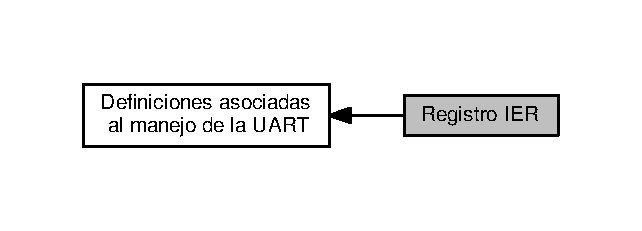
\includegraphics[width=308pt]{group___r_e_g_i_s_t_r_o___i_e_r}
\end{center}
\end{figure}
\subsection*{Macros}
\begin{DoxyCompactItemize}
\item 
\#define \hyperlink{group___r_e_g_i_s_t_r_o___i_e_r_ga6f8e43123ccd9f9be70e2e4e761fd8bf}{I\+E\+R\+\_\+\+R\+BR}~(0x01 $<$$<$ 0)
\begin{DoxyCompactList}\small\item\em R\+BR Interrupt Enable. Enables the Receive Data Available interrupt for U\+A\+RT. It also controls the Character Receive Time-\/out inturrupt. Reset Value \+: 0~\newline
 0 \+: Disable the R\+DA interrupt~\newline
 1 \+: Enable the R\+DA interrupt~\newline
. \end{DoxyCompactList}\item 
\#define \hyperlink{group___r_e_g_i_s_t_r_o___i_e_r_ga22682c3d4571d7a79ed0ca2bc88a15a6}{I\+E\+R\+\_\+\+T\+H\+RE}~(0x01 $<$$<$ 1)
\begin{DoxyCompactList}\small\item\em T\+H\+RE Interrupt Enable. Enables the T\+H\+RE interrupt for U\+A\+RT. The status of this interrupt can be read from U0\+L\+SR\mbox{[}5\mbox{]}.~\newline
 0 Disable the T\+H\+RE interrupt.~\newline
 1 Enable the T\+H\+RE interrupt.~\newline
. \end{DoxyCompactList}\item 
\#define \hyperlink{group___r_e_g_i_s_t_r_o___i_e_r_gaec947c63128590c8f615862ee9c2c953}{I\+E\+R\+\_\+\+R\+LS}~(0x01 $<$$<$ 2)
\begin{DoxyCompactList}\small\item\em RX Line Interrupt Enable. Enables the U\+A\+RT RX line status interrupts. The status of this interrupt can be read from U0\+L\+SR\mbox{[}4\+:1\mbox{]}.~\newline
 0 Disable the RX line status interrupts.~\newline
 1 Enable the RX line status interrupts.~\newline
. \end{DoxyCompactList}\end{DoxyCompactItemize}


\subsection{Detailed Description}
Definiciones asociadas al registro Interrupt Enable Register (U0\+I\+ER)~\newline
 Descripciones copiada directamente del manual U\+M10398 pag. 202. 

U\+A\+RT R\+LS interrupt (U0\+I\+IR\mbox{[}3\+:1\mbox{]} = 011) is the highest priority interrupt and is set whenever any one of four error conditions occur on the U\+A\+RT RX input\+: overrun error (OE), parity error (PE), framing error (FE) and break interrupt (BI). The U\+A\+RT Rx error condition that set the interrupt can be observed via U0\+L\+SR\mbox{[}4\+:1\mbox{]}. The interrupt is cleared upon a U0\+L\+SR read.~\newline
 U\+A\+RT R\+DA interrupt (U0\+I\+IR\mbox{[}3\+:1\mbox{]} = 010) shares the second level priority with the C\+TI interrupt (U0\+I\+IR\mbox{[}3\+:1\mbox{]} = 110). The R\+DA is activated when the U\+A\+RT Rx F\+I\+FO reaches the trigger level defined in U0\+F\+C\+R7\+:6 and is reset when the U\+A\+RT Rx F\+I\+FO depth falls below the trigger level. When the R\+DA interrupt goes active, the C\+PU can read a block of data defined by the trigger level.~\newline
 C\+TI interrupt (U0\+I\+IR\mbox{[}3\+:1\mbox{]} = 110) is a second level interrupt and is set when the U\+A\+RT Rx F\+I\+FO contains at least one character and no U\+A\+RT Rx F\+I\+FO activity has occurred in 3.\+5 to 4.\+5 character times. Any U\+A\+RT Rx F\+I\+FO activity (read or write of U\+A\+RT R\+SR) will clear the interrupt. This interrupt is intended to flush the U\+A\+RT R\+BR after a message has been received that is not a multiple of the trigger level size. For example, if a peripheral wished to send a 105 character message and the trigger level was 10 characters, the C\+PU would receive 10 R\+DA interrupts resulting in the transfer of 100 characters and 1 to 5 C\+TI interrupts (depending on the service routine) resulting in the transfer of the remaining 5 characters. ~\newline
~\newline
~\newline
 V\+ER T\+A\+B\+LA DE P\+R\+I\+O\+R\+I\+D\+A\+D\+ES P\+A\+G\+I\+NA 204 U\+M10398 

\subsection{Macro Definition Documentation}
\index{Registro I\+ER@{Registro I\+ER}!I\+E\+R\+\_\+\+R\+BR@{I\+E\+R\+\_\+\+R\+BR}}
\index{I\+E\+R\+\_\+\+R\+BR@{I\+E\+R\+\_\+\+R\+BR}!Registro I\+ER@{Registro I\+ER}}
\subsubsection[{\texorpdfstring{I\+E\+R\+\_\+\+R\+BR}{IER_RBR}}]{\setlength{\rightskip}{0pt plus 5cm}\#define I\+E\+R\+\_\+\+R\+BR~(0x01 $<$$<$ 0)}\hypertarget{group___r_e_g_i_s_t_r_o___i_e_r_ga6f8e43123ccd9f9be70e2e4e761fd8bf}{}\label{group___r_e_g_i_s_t_r_o___i_e_r_ga6f8e43123ccd9f9be70e2e4e761fd8bf}


R\+BR Interrupt Enable. Enables the Receive Data Available interrupt for U\+A\+RT. It also controls the Character Receive Time-\/out inturrupt. Reset Value \+: 0~\newline
 0 \+: Disable the R\+DA interrupt~\newline
 1 \+: Enable the R\+DA interrupt~\newline
. 



Definition at line 70 of file uart.\+h.

\index{Registro I\+ER@{Registro I\+ER}!I\+E\+R\+\_\+\+R\+LS@{I\+E\+R\+\_\+\+R\+LS}}
\index{I\+E\+R\+\_\+\+R\+LS@{I\+E\+R\+\_\+\+R\+LS}!Registro I\+ER@{Registro I\+ER}}
\subsubsection[{\texorpdfstring{I\+E\+R\+\_\+\+R\+LS}{IER_RLS}}]{\setlength{\rightskip}{0pt plus 5cm}\#define I\+E\+R\+\_\+\+R\+LS~(0x01 $<$$<$ 2)}\hypertarget{group___r_e_g_i_s_t_r_o___i_e_r_gaec947c63128590c8f615862ee9c2c953}{}\label{group___r_e_g_i_s_t_r_o___i_e_r_gaec947c63128590c8f615862ee9c2c953}


RX Line Interrupt Enable. Enables the U\+A\+RT RX line status interrupts. The status of this interrupt can be read from U0\+L\+SR\mbox{[}4\+:1\mbox{]}.~\newline
 0 Disable the RX line status interrupts.~\newline
 1 Enable the RX line status interrupts.~\newline
. 



Definition at line 86 of file uart.\+h.

\index{Registro I\+ER@{Registro I\+ER}!I\+E\+R\+\_\+\+T\+H\+RE@{I\+E\+R\+\_\+\+T\+H\+RE}}
\index{I\+E\+R\+\_\+\+T\+H\+RE@{I\+E\+R\+\_\+\+T\+H\+RE}!Registro I\+ER@{Registro I\+ER}}
\subsubsection[{\texorpdfstring{I\+E\+R\+\_\+\+T\+H\+RE}{IER_THRE}}]{\setlength{\rightskip}{0pt plus 5cm}\#define I\+E\+R\+\_\+\+T\+H\+RE~(0x01 $<$$<$ 1)}\hypertarget{group___r_e_g_i_s_t_r_o___i_e_r_ga22682c3d4571d7a79ed0ca2bc88a15a6}{}\label{group___r_e_g_i_s_t_r_o___i_e_r_ga22682c3d4571d7a79ed0ca2bc88a15a6}


T\+H\+RE Interrupt Enable. Enables the T\+H\+RE interrupt for U\+A\+RT. The status of this interrupt can be read from U0\+L\+SR\mbox{[}5\mbox{]}.~\newline
 0 Disable the T\+H\+RE interrupt.~\newline
 1 Enable the T\+H\+RE interrupt.~\newline
. 



Definition at line 78 of file uart.\+h.


\hypertarget{group___r_e_g_i_s_t_r_o___i_i_r}{}\section{Registro I\+IR}
\label{group___r_e_g_i_s_t_r_o___i_i_r}\index{Registro I\+IR@{Registro I\+IR}}


Definiciones asociadas al registro Interrupt Enable Register (U0\+I\+ER)~\newline
 Descripciones copiada directamente del manual U\+M10398 pag. 203.  


Collaboration diagram for Registro I\+IR\+:\nopagebreak
\begin{figure}[H]
\begin{center}
\leavevmode
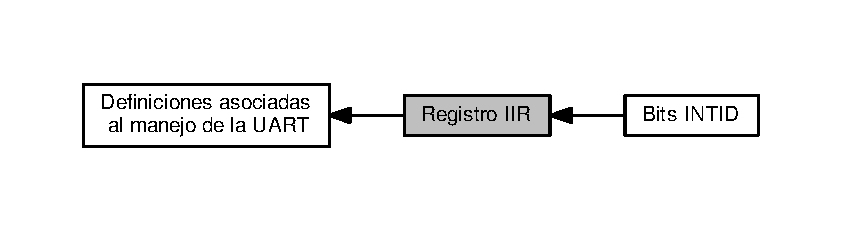
\includegraphics[width=350pt]{group___r_e_g_i_s_t_r_o___i_i_r}
\end{center}
\end{figure}
\subsection*{Modules}
\begin{DoxyCompactItemize}
\item 
\hyperlink{group___i_n_t_i_d}{Bits I\+N\+T\+ID}
\begin{DoxyCompactList}\small\item\em Interrupt identification.~\newline
 {\bfseries  U0\+I\+ER\mbox{[}3\+:1\mbox{]} } identifies an interrupt 0 corresponding to the U\+A\+RT Rx F\+I\+FO. All other combinations of U0\+I\+ER\mbox{[}3\+:1\mbox{]} not listed below are reserved (100,101,111). \end{DoxyCompactList}\end{DoxyCompactItemize}
\subsection*{Macros}
\begin{DoxyCompactItemize}
\item 
\#define \hyperlink{group___r_e_g_i_s_t_r_o___i_i_r_gaceec69c2af58ca0d5bc80828b2a58964}{I\+I\+R\+\_\+\+P\+E\+ND}~(0x01 $<$$<$ 0)
\begin{DoxyCompactList}\small\item\em Interrupt status. Note that U0\+I\+IR\mbox{[}0\mbox{]} is active low. The pending interrupt can be determined by evaluating U0\+I\+IR\mbox{[}3\+:1\mbox{]}.~\newline
 0 At least one interrupt is pending. ~\newline
 1 No interrupt is pending. ~\newline
. \end{DoxyCompactList}\end{DoxyCompactItemize}


\subsection{Detailed Description}
Definiciones asociadas al registro Interrupt Enable Register (U0\+I\+ER)~\newline
 Descripciones copiada directamente del manual U\+M10398 pag. 203. 



\subsection{Macro Definition Documentation}
\index{Registro I\+IR@{Registro I\+IR}!I\+I\+R\+\_\+\+P\+E\+ND@{I\+I\+R\+\_\+\+P\+E\+ND}}
\index{I\+I\+R\+\_\+\+P\+E\+ND@{I\+I\+R\+\_\+\+P\+E\+ND}!Registro I\+IR@{Registro I\+IR}}
\subsubsection[{\texorpdfstring{I\+I\+R\+\_\+\+P\+E\+ND}{IIR_PEND}}]{\setlength{\rightskip}{0pt plus 5cm}\#define I\+I\+R\+\_\+\+P\+E\+ND~(0x01 $<$$<$ 0)}\hypertarget{group___r_e_g_i_s_t_r_o___i_i_r_gaceec69c2af58ca0d5bc80828b2a58964}{}\label{group___r_e_g_i_s_t_r_o___i_i_r_gaceec69c2af58ca0d5bc80828b2a58964}


Interrupt status. Note that U0\+I\+IR\mbox{[}0\mbox{]} is active low. The pending interrupt can be determined by evaluating U0\+I\+IR\mbox{[}3\+:1\mbox{]}.~\newline
 0 At least one interrupt is pending. ~\newline
 1 No interrupt is pending. ~\newline
. 



Definition at line 107 of file uart.\+h.


\hypertarget{group___i_n_t_i_d}{}\section{Bits I\+N\+T\+ID}
\label{group___i_n_t_i_d}\index{Bits I\+N\+T\+ID@{Bits I\+N\+T\+ID}}


Interrupt identification.~\newline
 {\bfseries  U0\+I\+ER\mbox{[}3\+:1\mbox{]} } identifies an interrupt 0 corresponding to the U\+A\+RT Rx F\+I\+FO. All other combinations of U0\+I\+ER\mbox{[}3\+:1\mbox{]} not listed below are reserved (100,101,111).  


Collaboration diagram for Bits I\+N\+T\+ID\+:\nopagebreak
\begin{figure}[H]
\begin{center}
\leavevmode
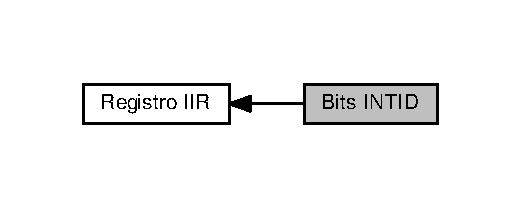
\includegraphics[width=250pt]{group___i_n_t_i_d}
\end{center}
\end{figure}
\subsection*{Macros}
\begin{DoxyCompactItemize}
\item 
\#define \hyperlink{group___i_n_t_i_d_ga03db7def835d2e60f1cc7470bdf35b08}{I\+I\+R\+\_\+\+R\+LS}~0x03
\begin{DoxyCompactList}\small\item\em 1 -\/ Receive Line Status (R\+LS). \end{DoxyCompactList}\item 
\#define \hyperlink{group___i_n_t_i_d_ga80925dd3aa4708e148a9d63088b4758d}{I\+I\+R\+\_\+\+R\+DA}~0x02
\begin{DoxyCompactList}\small\item\em 2a -\/ Receive Data Available (R\+DA). \end{DoxyCompactList}\item 
\#define \hyperlink{group___i_n_t_i_d_ga4842d23857b5599cf59365f23a46722f}{I\+I\+R\+\_\+\+C\+TI}~0x06
\begin{DoxyCompactList}\small\item\em 2b -\/ Character Time-\/out Indicator (C\+TI). \end{DoxyCompactList}\item 
\#define \hyperlink{group___i_n_t_i_d_gafbff8bd626a8fce1f6082d355000c2b2}{I\+I\+R\+\_\+\+T\+H\+RE}~0x01
\begin{DoxyCompactList}\small\item\em 3 -\/ T\+H\+RE Interrupt. \end{DoxyCompactList}\end{DoxyCompactItemize}


\subsection{Detailed Description}
Interrupt identification.~\newline
 {\bfseries  U0\+I\+ER\mbox{[}3\+:1\mbox{]} } identifies an interrupt 0 corresponding to the U\+A\+RT Rx F\+I\+FO. All other combinations of U0\+I\+ER\mbox{[}3\+:1\mbox{]} not listed below are reserved (100,101,111). 



\subsection{Macro Definition Documentation}
\index{Bits I\+N\+T\+ID@{Bits I\+N\+T\+ID}!I\+I\+R\+\_\+\+C\+TI@{I\+I\+R\+\_\+\+C\+TI}}
\index{I\+I\+R\+\_\+\+C\+TI@{I\+I\+R\+\_\+\+C\+TI}!Bits I\+N\+T\+ID@{Bits I\+N\+T\+ID}}
\subsubsection[{\texorpdfstring{I\+I\+R\+\_\+\+C\+TI}{IIR_CTI}}]{\setlength{\rightskip}{0pt plus 5cm}\#define I\+I\+R\+\_\+\+C\+TI~0x06}\hypertarget{group___i_n_t_i_d_ga4842d23857b5599cf59365f23a46722f}{}\label{group___i_n_t_i_d_ga4842d23857b5599cf59365f23a46722f}


2b -\/ Character Time-\/out Indicator (C\+TI). 



Definition at line 122 of file uart.\+h.

\index{Bits I\+N\+T\+ID@{Bits I\+N\+T\+ID}!I\+I\+R\+\_\+\+R\+DA@{I\+I\+R\+\_\+\+R\+DA}}
\index{I\+I\+R\+\_\+\+R\+DA@{I\+I\+R\+\_\+\+R\+DA}!Bits I\+N\+T\+ID@{Bits I\+N\+T\+ID}}
\subsubsection[{\texorpdfstring{I\+I\+R\+\_\+\+R\+DA}{IIR_RDA}}]{\setlength{\rightskip}{0pt plus 5cm}\#define I\+I\+R\+\_\+\+R\+DA~0x02}\hypertarget{group___i_n_t_i_d_ga80925dd3aa4708e148a9d63088b4758d}{}\label{group___i_n_t_i_d_ga80925dd3aa4708e148a9d63088b4758d}


2a -\/ Receive Data Available (R\+DA). 



Definition at line 120 of file uart.\+h.

\index{Bits I\+N\+T\+ID@{Bits I\+N\+T\+ID}!I\+I\+R\+\_\+\+R\+LS@{I\+I\+R\+\_\+\+R\+LS}}
\index{I\+I\+R\+\_\+\+R\+LS@{I\+I\+R\+\_\+\+R\+LS}!Bits I\+N\+T\+ID@{Bits I\+N\+T\+ID}}
\subsubsection[{\texorpdfstring{I\+I\+R\+\_\+\+R\+LS}{IIR_RLS}}]{\setlength{\rightskip}{0pt plus 5cm}\#define I\+I\+R\+\_\+\+R\+LS~0x03}\hypertarget{group___i_n_t_i_d_ga03db7def835d2e60f1cc7470bdf35b08}{}\label{group___i_n_t_i_d_ga03db7def835d2e60f1cc7470bdf35b08}


1 -\/ Receive Line Status (R\+LS). 



Definition at line 118 of file uart.\+h.

\index{Bits I\+N\+T\+ID@{Bits I\+N\+T\+ID}!I\+I\+R\+\_\+\+T\+H\+RE@{I\+I\+R\+\_\+\+T\+H\+RE}}
\index{I\+I\+R\+\_\+\+T\+H\+RE@{I\+I\+R\+\_\+\+T\+H\+RE}!Bits I\+N\+T\+ID@{Bits I\+N\+T\+ID}}
\subsubsection[{\texorpdfstring{I\+I\+R\+\_\+\+T\+H\+RE}{IIR_THRE}}]{\setlength{\rightskip}{0pt plus 5cm}\#define I\+I\+R\+\_\+\+T\+H\+RE~0x01}\hypertarget{group___i_n_t_i_d_gafbff8bd626a8fce1f6082d355000c2b2}{}\label{group___i_n_t_i_d_gafbff8bd626a8fce1f6082d355000c2b2}


3 -\/ T\+H\+RE Interrupt. 



Definition at line 124 of file uart.\+h.


\hypertarget{group___r_e_g_i_s_t_r_o___l_s_r}{}\section{Registro L\+SR}
\label{group___r_e_g_i_s_t_r_o___l_s_r}\index{Registro L\+SR@{Registro L\+SR}}


Definiciones asociadas al registro Line Status Register (U0\+L\+SR)~\newline
 Descripciones copiada directamente del manual U\+M10398 pag. 210~\newline
 The U0\+L\+SR is a Read Only register that provides status information on the U\+A\+RT TX and RX blocks.~\newline
.  


Collaboration diagram for Registro L\+SR\+:\nopagebreak
\begin{figure}[H]
\begin{center}
\leavevmode
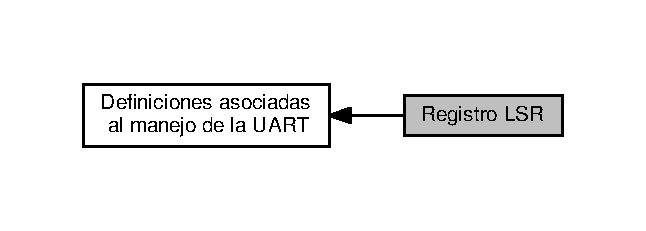
\includegraphics[width=310pt]{group___r_e_g_i_s_t_r_o___l_s_r}
\end{center}
\end{figure}
\subsection*{Macros}
\begin{DoxyCompactItemize}
\item 
\#define \hyperlink{group___r_e_g_i_s_t_r_o___l_s_r_ga9e3adac29ef2f5d2cf60c4cebe971de9}{L\+S\+R\+\_\+\+R\+DR}~0x01
\begin{DoxyCompactList}\small\item\em Receiver Data Ready. U0\+L\+SR\mbox{[}0\mbox{]} is set when the U0\+R\+BR holds 0 an unread character and is cleared when the U\+A\+RT R\+BR F\+I\+FO is empty.~\newline
 0 U0\+R\+BR is empty.~\newline
 1 U0\+R\+BR contains valid data.~\newline
. \end{DoxyCompactList}\item 
\#define \hyperlink{group___r_e_g_i_s_t_r_o___l_s_r_gae844dd49bb0e0770bcf46ad5bfe20973}{L\+S\+R\+\_\+\+OE}~0x02
\begin{DoxyCompactList}\small\item\em Overrun Error. The overrun error condition is set as soon as it 0 occurs. A U0\+L\+SR read clears U0\+L\+SR\mbox{[}1\mbox{]}. U0\+L\+SR\mbox{[}1\mbox{]} is set when U\+A\+RT R\+SR has a new character assembled and the U\+A\+RT R\+BR F\+I\+FO is full. In this case, the U\+A\+RT R\+BR F\+I\+FO will not be overwritten and the character in the U\+A\+RT R\+SR will be lost.~\newline
 0 Overrun error status is inactive.~\newline
 1 Overrun error status is active.~\newline
. \end{DoxyCompactList}\item 
\#define \hyperlink{group___r_e_g_i_s_t_r_o___l_s_r_ga0ee28cdbc0917173f06cc39527452a8f}{L\+S\+R\+\_\+\+PE}~0x04
\begin{DoxyCompactList}\small\item\em Parity Error. When the parity bit of a received character is in the wrong state, a parity error occurs. A U0\+L\+SR read clears U0\+L\+SR\mbox{[}2\mbox{]}. Time of parity error detection is dependent on U0\+F\+CR\mbox{[}0\mbox{]}.~\newline
 0 Parity error status is inactive.~\newline
 1 Parity error status is active.~\newline
. \end{DoxyCompactList}\item 
\#define \hyperlink{group___r_e_g_i_s_t_r_o___l_s_r_gae3f9ccc88c615d1257ad400cf27af7eb}{L\+S\+R\+\_\+\+FE}~0x08
\begin{DoxyCompactList}\small\item\em Framing Error. When the stop bit of a received character is a 0 logic 0, a framing error occurs. A U0\+L\+SR read clears U0\+L\+SR\mbox{[}3\mbox{]}. The time of the framing error detection is dependent on U0\+F\+C\+R0. Upon detection of a framing error, the RX will attempt to re-\/synchronize to the data and assume that the bad stop bit is actually an early start bit. However, it cannot be assumed that the next received byte will be correct even if there is no Framing Error. Note\+: A framing error is associated with the character at the top of the U\+A\+RT R\+BR F\+I\+FO.~\newline
. \end{DoxyCompactList}\item 
\#define \hyperlink{group___r_e_g_i_s_t_r_o___l_s_r_ga0fa2f414cac085b768774f2881321b60}{L\+S\+R\+\_\+\+BI}~0x10
\begin{DoxyCompactList}\small\item\em Break Interrupt. When R\+X\+D1 is held in the spacing state (all zeros) for one full character transmission (start, data, parity, stop), a break interrupt occurs. Once the break condition has been detected, the receiver goes idle until R\+X\+D1 goes to marking state (all ones). A U0\+L\+SR read clears this status bit. The time of break detection is dependent on U0\+F\+CR\mbox{[}0\mbox{]}.~\newline
 0 Note\+: The break interrupt is associated with the character at the top of the U\+A\+RT R\+BR F\+I\+FO.~\newline
. \end{DoxyCompactList}\item 
\#define \hyperlink{group___r_e_g_i_s_t_r_o___l_s_r_ga8c1a828f5fe296a9c1668cf3e72c00c1}{L\+S\+R\+\_\+\+T\+H\+RE}~0x20
\begin{DoxyCompactList}\small\item\em Transmitter Holding Register Empty. T\+H\+RE is set immediately 1 upon detection of an empty U\+A\+RT T\+HR and is cleared on a U0\+T\+HR write.~\newline
. \end{DoxyCompactList}\item 
\#define \hyperlink{group___r_e_g_i_s_t_r_o___l_s_r_ga7dfceb10f5c20011b9410e2efb39163d}{L\+S\+R\+\_\+\+T\+E\+MT}~0x40
\begin{DoxyCompactList}\small\item\em Transmitter Empty. T\+E\+MT is set when both U0\+T\+HR and U0\+T\+SR are empty; T\+E\+MT is cleared when either the U0\+T\+SR or the U0\+T\+HR contain valid data. This bit is updated as soon as 50 \% of the first stop bit has been transmitted or a byte has been written into the T\+HR.~\newline
. \end{DoxyCompactList}\item 
\#define \hyperlink{group___r_e_g_i_s_t_r_o___l_s_r_gad481ff8993ac05c71d4ca3b611833df0}{L\+S\+R\+\_\+\+R\+X\+FE}~0x80
\begin{DoxyCompactList}\small\item\em Error in RX F\+I\+FO. U0\+L\+SR\mbox{[}7\mbox{]} is set when a character with a RX 0 error such as framing error, parity error or break interrupt, is loaded into the U0\+R\+BR. This bit is cleared when the U0\+L\+SR register is read and there are no subsequent errors in the U\+A\+RT F\+I\+FO.~\newline
. \end{DoxyCompactList}\end{DoxyCompactItemize}


\subsection{Detailed Description}
Definiciones asociadas al registro Line Status Register (U0\+L\+SR)~\newline
 Descripciones copiada directamente del manual U\+M10398 pag. 210~\newline
 The U0\+L\+SR is a Read Only register that provides status information on the U\+A\+RT TX and RX blocks.~\newline
. 



\subsection{Macro Definition Documentation}
\index{Registro L\+SR@{Registro L\+SR}!L\+S\+R\+\_\+\+BI@{L\+S\+R\+\_\+\+BI}}
\index{L\+S\+R\+\_\+\+BI@{L\+S\+R\+\_\+\+BI}!Registro L\+SR@{Registro L\+SR}}
\subsubsection[{\texorpdfstring{L\+S\+R\+\_\+\+BI}{LSR_BI}}]{\setlength{\rightskip}{0pt plus 5cm}\#define L\+S\+R\+\_\+\+BI~0x10}\hypertarget{group___r_e_g_i_s_t_r_o___l_s_r_ga0fa2f414cac085b768774f2881321b60}{}\label{group___r_e_g_i_s_t_r_o___l_s_r_ga0fa2f414cac085b768774f2881321b60}


Break Interrupt. When R\+X\+D1 is held in the spacing state (all zeros) for one full character transmission (start, data, parity, stop), a break interrupt occurs. Once the break condition has been detected, the receiver goes idle until R\+X\+D1 goes to marking state (all ones). A U0\+L\+SR read clears this status bit. The time of break detection is dependent on U0\+F\+CR\mbox{[}0\mbox{]}.~\newline
 0 Note\+: The break interrupt is associated with the character at the top of the U\+A\+RT R\+BR F\+I\+FO.~\newline
. 

0 Break interrupt status is inactive.~\newline
 1 Break interrupt status is active.~\newline


Definition at line 204 of file uart.\+h.

\index{Registro L\+SR@{Registro L\+SR}!L\+S\+R\+\_\+\+FE@{L\+S\+R\+\_\+\+FE}}
\index{L\+S\+R\+\_\+\+FE@{L\+S\+R\+\_\+\+FE}!Registro L\+SR@{Registro L\+SR}}
\subsubsection[{\texorpdfstring{L\+S\+R\+\_\+\+FE}{LSR_FE}}]{\setlength{\rightskip}{0pt plus 5cm}\#define L\+S\+R\+\_\+\+FE~0x08}\hypertarget{group___r_e_g_i_s_t_r_o___l_s_r_gae3f9ccc88c615d1257ad400cf27af7eb}{}\label{group___r_e_g_i_s_t_r_o___l_s_r_gae3f9ccc88c615d1257ad400cf27af7eb}


Framing Error. When the stop bit of a received character is a 0 logic 0, a framing error occurs. A U0\+L\+SR read clears U0\+L\+SR\mbox{[}3\mbox{]}. The time of the framing error detection is dependent on U0\+F\+C\+R0. Upon detection of a framing error, the RX will attempt to re-\/synchronize to the data and assume that the bad stop bit is actually an early start bit. However, it cannot be assumed that the next received byte will be correct even if there is no Framing Error. Note\+: A framing error is associated with the character at the top of the U\+A\+RT R\+BR F\+I\+FO.~\newline
. 

0 Framing error status is inactive.~\newline
 1 Framing error status is active.~\newline


Definition at line 188 of file uart.\+h.

\index{Registro L\+SR@{Registro L\+SR}!L\+S\+R\+\_\+\+OE@{L\+S\+R\+\_\+\+OE}}
\index{L\+S\+R\+\_\+\+OE@{L\+S\+R\+\_\+\+OE}!Registro L\+SR@{Registro L\+SR}}
\subsubsection[{\texorpdfstring{L\+S\+R\+\_\+\+OE}{LSR_OE}}]{\setlength{\rightskip}{0pt plus 5cm}\#define L\+S\+R\+\_\+\+OE~0x02}\hypertarget{group___r_e_g_i_s_t_r_o___l_s_r_gae844dd49bb0e0770bcf46ad5bfe20973}{}\label{group___r_e_g_i_s_t_r_o___l_s_r_gae844dd49bb0e0770bcf46ad5bfe20973}


Overrun Error. The overrun error condition is set as soon as it 0 occurs. A U0\+L\+SR read clears U0\+L\+SR\mbox{[}1\mbox{]}. U0\+L\+SR\mbox{[}1\mbox{]} is set when U\+A\+RT R\+SR has a new character assembled and the U\+A\+RT R\+BR F\+I\+FO is full. In this case, the U\+A\+RT R\+BR F\+I\+FO will not be overwritten and the character in the U\+A\+RT R\+SR will be lost.~\newline
 0 Overrun error status is inactive.~\newline
 1 Overrun error status is active.~\newline
. 



Definition at line 162 of file uart.\+h.

\index{Registro L\+SR@{Registro L\+SR}!L\+S\+R\+\_\+\+PE@{L\+S\+R\+\_\+\+PE}}
\index{L\+S\+R\+\_\+\+PE@{L\+S\+R\+\_\+\+PE}!Registro L\+SR@{Registro L\+SR}}
\subsubsection[{\texorpdfstring{L\+S\+R\+\_\+\+PE}{LSR_PE}}]{\setlength{\rightskip}{0pt plus 5cm}\#define L\+S\+R\+\_\+\+PE~0x04}\hypertarget{group___r_e_g_i_s_t_r_o___l_s_r_ga0ee28cdbc0917173f06cc39527452a8f}{}\label{group___r_e_g_i_s_t_r_o___l_s_r_ga0ee28cdbc0917173f06cc39527452a8f}


Parity Error. When the parity bit of a received character is in the wrong state, a parity error occurs. A U0\+L\+SR read clears U0\+L\+SR\mbox{[}2\mbox{]}. Time of parity error detection is dependent on U0\+F\+CR\mbox{[}0\mbox{]}.~\newline
 0 Parity error status is inactive.~\newline
 1 Parity error status is active.~\newline
. 



Definition at line 171 of file uart.\+h.

\index{Registro L\+SR@{Registro L\+SR}!L\+S\+R\+\_\+\+R\+DR@{L\+S\+R\+\_\+\+R\+DR}}
\index{L\+S\+R\+\_\+\+R\+DR@{L\+S\+R\+\_\+\+R\+DR}!Registro L\+SR@{Registro L\+SR}}
\subsubsection[{\texorpdfstring{L\+S\+R\+\_\+\+R\+DR}{LSR_RDR}}]{\setlength{\rightskip}{0pt plus 5cm}\#define L\+S\+R\+\_\+\+R\+DR~0x01}\hypertarget{group___r_e_g_i_s_t_r_o___l_s_r_ga9e3adac29ef2f5d2cf60c4cebe971de9}{}\label{group___r_e_g_i_s_t_r_o___l_s_r_ga9e3adac29ef2f5d2cf60c4cebe971de9}


Receiver Data Ready. U0\+L\+SR\mbox{[}0\mbox{]} is set when the U0\+R\+BR holds 0 an unread character and is cleared when the U\+A\+RT R\+BR F\+I\+FO is empty.~\newline
 0 U0\+R\+BR is empty.~\newline
 1 U0\+R\+BR contains valid data.~\newline
. 



Definition at line 152 of file uart.\+h.

\index{Registro L\+SR@{Registro L\+SR}!L\+S\+R\+\_\+\+R\+X\+FE@{L\+S\+R\+\_\+\+R\+X\+FE}}
\index{L\+S\+R\+\_\+\+R\+X\+FE@{L\+S\+R\+\_\+\+R\+X\+FE}!Registro L\+SR@{Registro L\+SR}}
\subsubsection[{\texorpdfstring{L\+S\+R\+\_\+\+R\+X\+FE}{LSR_RXFE}}]{\setlength{\rightskip}{0pt plus 5cm}\#define L\+S\+R\+\_\+\+R\+X\+FE~0x80}\hypertarget{group___r_e_g_i_s_t_r_o___l_s_r_gad481ff8993ac05c71d4ca3b611833df0}{}\label{group___r_e_g_i_s_t_r_o___l_s_r_gad481ff8993ac05c71d4ca3b611833df0}


Error in RX F\+I\+FO. U0\+L\+SR\mbox{[}7\mbox{]} is set when a character with a RX 0 error such as framing error, parity error or break interrupt, is loaded into the U0\+R\+BR. This bit is cleared when the U0\+L\+SR register is read and there are no subsequent errors in the U\+A\+RT F\+I\+FO.~\newline
. 

0 U0\+R\+BR contains no U\+A\+RT RX errors or U0\+F\+CR\mbox{[}0\mbox{]}=0.~\newline
 1 U\+A\+RT R\+BR contains at least one U\+A\+RT RX error.~\newline


Definition at line 237 of file uart.\+h.

\index{Registro L\+SR@{Registro L\+SR}!L\+S\+R\+\_\+\+T\+E\+MT@{L\+S\+R\+\_\+\+T\+E\+MT}}
\index{L\+S\+R\+\_\+\+T\+E\+MT@{L\+S\+R\+\_\+\+T\+E\+MT}!Registro L\+SR@{Registro L\+SR}}
\subsubsection[{\texorpdfstring{L\+S\+R\+\_\+\+T\+E\+MT}{LSR_TEMT}}]{\setlength{\rightskip}{0pt plus 5cm}\#define L\+S\+R\+\_\+\+T\+E\+MT~0x40}\hypertarget{group___r_e_g_i_s_t_r_o___l_s_r_ga7dfceb10f5c20011b9410e2efb39163d}{}\label{group___r_e_g_i_s_t_r_o___l_s_r_ga7dfceb10f5c20011b9410e2efb39163d}


Transmitter Empty. T\+E\+MT is set when both U0\+T\+HR and U0\+T\+SR are empty; T\+E\+MT is cleared when either the U0\+T\+SR or the U0\+T\+HR contain valid data. This bit is updated as soon as 50 \% of the first stop bit has been transmitted or a byte has been written into the T\+HR.~\newline
. 

0 U0\+T\+HR and/or the U0\+T\+SR contains valid data.~\newline
 1 U0\+T\+HR and the U0\+T\+SR are empty.~\newline


Definition at line 225 of file uart.\+h.

\index{Registro L\+SR@{Registro L\+SR}!L\+S\+R\+\_\+\+T\+H\+RE@{L\+S\+R\+\_\+\+T\+H\+RE}}
\index{L\+S\+R\+\_\+\+T\+H\+RE@{L\+S\+R\+\_\+\+T\+H\+RE}!Registro L\+SR@{Registro L\+SR}}
\subsubsection[{\texorpdfstring{L\+S\+R\+\_\+\+T\+H\+RE}{LSR_THRE}}]{\setlength{\rightskip}{0pt plus 5cm}\#define L\+S\+R\+\_\+\+T\+H\+RE~0x20}\hypertarget{group___r_e_g_i_s_t_r_o___l_s_r_ga8c1a828f5fe296a9c1668cf3e72c00c1}{}\label{group___r_e_g_i_s_t_r_o___l_s_r_ga8c1a828f5fe296a9c1668cf3e72c00c1}


Transmitter Holding Register Empty. T\+H\+RE is set immediately 1 upon detection of an empty U\+A\+RT T\+HR and is cleared on a U0\+T\+HR write.~\newline
. 

0 U0\+T\+HR contains valid data.~\newline
 1 U0\+T\+HR is empty.~\newline


Definition at line 213 of file uart.\+h.


\hypertarget{group___r_s485_m_o_d_e}{}\section{R\+S485 mode definition.}
\label{group___r_s485_m_o_d_e}\index{R\+S485 mode definition.@{R\+S485 mode definition.}}


The U0\+R\+S485\+C\+T\+RL register controls the configuration of the U\+A\+RT in R\+S-\/485/\+E\+I\+A-\/485 mode.  


Collaboration diagram for R\+S485 mode definition.\+:\nopagebreak
\begin{figure}[H]
\begin{center}
\leavevmode
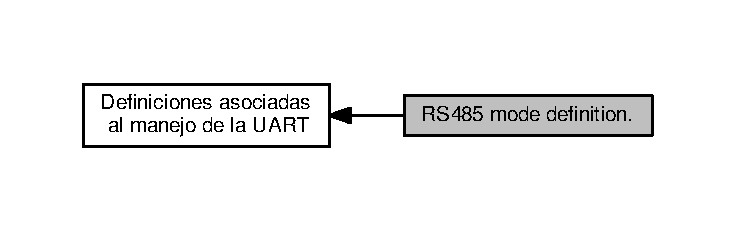
\includegraphics[width=350pt]{group___r_s485_m_o_d_e}
\end{center}
\end{figure}
\subsection*{Macros}
\begin{DoxyCompactItemize}
\item 
\#define \hyperlink{group___r_s485_m_o_d_e_ga124bdfe48f8f5794d2ce15f7de7120ff}{R\+S485\+\_\+\+N\+M\+M\+EN}~(0x1 $<$$<$ 0)
\begin{DoxyCompactList}\small\item\em Habilita el modo multipunto. Se envían las direcciones al bus con error de paridad para generar una I\+RQ de la U\+A\+RT. \end{DoxyCompactList}\item 
\#define \hyperlink{group___r_s485_m_o_d_e_ga6dd71ac874eee782a027c667162d2401}{R\+S485\+\_\+\+R\+X\+D\+IS}~(0x1 $<$$<$ 1)
\begin{DoxyCompactList}\small\item\em Habilita la recepción de datos. \end{DoxyCompactList}\item 
\#define \hyperlink{group___r_s485_m_o_d_e_ga1b63fc40ac9dea74f6a3822c7e45a0b1}{R\+S485\+\_\+\+A\+A\+D\+EN}~(0x1 $<$$<$ 2)
\begin{DoxyCompactList}\small\item\em Deteccion automática de dirección (A\+AD) habilitada. \end{DoxyCompactList}\item 
\#define \hyperlink{group___r_s485_m_o_d_e_gaab560420636565a39ce5ddc3539438b3}{R\+S485\+\_\+\+S\+EL}~(0x1 $<$$<$ 3)
\begin{DoxyCompactList}\small\item\em Determina el pin de direccion -\/$>$ 0 \+: R\+TS negado P1.\+5 (J21) // 1 \+: D\+TR negado P3.\+0 (J25) \end{DoxyCompactList}\item 
\#define \hyperlink{group___r_s485_m_o_d_e_gad273c8e4d740c13bd42b605f01c7602a}{R\+S485\+\_\+\+D\+C\+T\+RL}~(0x1 $<$$<$ 4)
\begin{DoxyCompactList}\small\item\em Habilita el control automático de dirección. \end{DoxyCompactList}\item 
\#define \hyperlink{group___r_s485_m_o_d_e_ga4067a15fda5fce2f25e4e722067d41d7}{R\+S485\+\_\+\+O\+I\+NV}~(0x1 $<$$<$ 5)
\begin{DoxyCompactList}\small\item\em 0 \+: El pin de control se pone en 0 cuando se esta por transmitir. Se pone en 1 al terminar la transmision 1 \+: El pin de control se pone en 1 cuando se esta por transmitir. Se pone en 0 al terminar la transmision \end{DoxyCompactList}\end{DoxyCompactItemize}


\subsection{Detailed Description}
The U0\+R\+S485\+C\+T\+RL register controls the configuration of the U\+A\+RT in R\+S-\/485/\+E\+I\+A-\/485 mode. 



\subsection{Macro Definition Documentation}
\index{R\+S485 mode definition.@{R\+S485 mode definition.}!R\+S485\+\_\+\+A\+A\+D\+EN@{R\+S485\+\_\+\+A\+A\+D\+EN}}
\index{R\+S485\+\_\+\+A\+A\+D\+EN@{R\+S485\+\_\+\+A\+A\+D\+EN}!R\+S485 mode definition.@{R\+S485 mode definition.}}
\subsubsection[{\texorpdfstring{R\+S485\+\_\+\+A\+A\+D\+EN}{RS485_AADEN}}]{\setlength{\rightskip}{0pt plus 5cm}\#define R\+S485\+\_\+\+A\+A\+D\+EN~(0x1 $<$$<$ 2)}\hypertarget{group___r_s485_m_o_d_e_ga1b63fc40ac9dea74f6a3822c7e45a0b1}{}\label{group___r_s485_m_o_d_e_ga1b63fc40ac9dea74f6a3822c7e45a0b1}


Deteccion automática de dirección (A\+AD) habilitada. 



Definition at line 260 of file uart.\+h.

\index{R\+S485 mode definition.@{R\+S485 mode definition.}!R\+S485\+\_\+\+D\+C\+T\+RL@{R\+S485\+\_\+\+D\+C\+T\+RL}}
\index{R\+S485\+\_\+\+D\+C\+T\+RL@{R\+S485\+\_\+\+D\+C\+T\+RL}!R\+S485 mode definition.@{R\+S485 mode definition.}}
\subsubsection[{\texorpdfstring{R\+S485\+\_\+\+D\+C\+T\+RL}{RS485_DCTRL}}]{\setlength{\rightskip}{0pt plus 5cm}\#define R\+S485\+\_\+\+D\+C\+T\+RL~(0x1 $<$$<$ 4)}\hypertarget{group___r_s485_m_o_d_e_gad273c8e4d740c13bd42b605f01c7602a}{}\label{group___r_s485_m_o_d_e_gad273c8e4d740c13bd42b605f01c7602a}


Habilita el control automático de dirección. 



Definition at line 264 of file uart.\+h.

\index{R\+S485 mode definition.@{R\+S485 mode definition.}!R\+S485\+\_\+\+N\+M\+M\+EN@{R\+S485\+\_\+\+N\+M\+M\+EN}}
\index{R\+S485\+\_\+\+N\+M\+M\+EN@{R\+S485\+\_\+\+N\+M\+M\+EN}!R\+S485 mode definition.@{R\+S485 mode definition.}}
\subsubsection[{\texorpdfstring{R\+S485\+\_\+\+N\+M\+M\+EN}{RS485_NMMEN}}]{\setlength{\rightskip}{0pt plus 5cm}\#define R\+S485\+\_\+\+N\+M\+M\+EN~(0x1 $<$$<$ 0)}\hypertarget{group___r_s485_m_o_d_e_ga124bdfe48f8f5794d2ce15f7de7120ff}{}\label{group___r_s485_m_o_d_e_ga124bdfe48f8f5794d2ce15f7de7120ff}


Habilita el modo multipunto. Se envían las direcciones al bus con error de paridad para generar una I\+RQ de la U\+A\+RT. 



Definition at line 256 of file uart.\+h.

\index{R\+S485 mode definition.@{R\+S485 mode definition.}!R\+S485\+\_\+\+O\+I\+NV@{R\+S485\+\_\+\+O\+I\+NV}}
\index{R\+S485\+\_\+\+O\+I\+NV@{R\+S485\+\_\+\+O\+I\+NV}!R\+S485 mode definition.@{R\+S485 mode definition.}}
\subsubsection[{\texorpdfstring{R\+S485\+\_\+\+O\+I\+NV}{RS485_OINV}}]{\setlength{\rightskip}{0pt plus 5cm}\#define R\+S485\+\_\+\+O\+I\+NV~(0x1 $<$$<$ 5)}\hypertarget{group___r_s485_m_o_d_e_ga4067a15fda5fce2f25e4e722067d41d7}{}\label{group___r_s485_m_o_d_e_ga4067a15fda5fce2f25e4e722067d41d7}


0 \+: El pin de control se pone en 0 cuando se esta por transmitir. Se pone en 1 al terminar la transmision 1 \+: El pin de control se pone en 1 cuando se esta por transmitir. Se pone en 0 al terminar la transmision 



Definition at line 268 of file uart.\+h.

\index{R\+S485 mode definition.@{R\+S485 mode definition.}!R\+S485\+\_\+\+R\+X\+D\+IS@{R\+S485\+\_\+\+R\+X\+D\+IS}}
\index{R\+S485\+\_\+\+R\+X\+D\+IS@{R\+S485\+\_\+\+R\+X\+D\+IS}!R\+S485 mode definition.@{R\+S485 mode definition.}}
\subsubsection[{\texorpdfstring{R\+S485\+\_\+\+R\+X\+D\+IS}{RS485_RXDIS}}]{\setlength{\rightskip}{0pt plus 5cm}\#define R\+S485\+\_\+\+R\+X\+D\+IS~(0x1 $<$$<$ 1)}\hypertarget{group___r_s485_m_o_d_e_ga6dd71ac874eee782a027c667162d2401}{}\label{group___r_s485_m_o_d_e_ga6dd71ac874eee782a027c667162d2401}


Habilita la recepción de datos. 



Definition at line 258 of file uart.\+h.

\index{R\+S485 mode definition.@{R\+S485 mode definition.}!R\+S485\+\_\+\+S\+EL@{R\+S485\+\_\+\+S\+EL}}
\index{R\+S485\+\_\+\+S\+EL@{R\+S485\+\_\+\+S\+EL}!R\+S485 mode definition.@{R\+S485 mode definition.}}
\subsubsection[{\texorpdfstring{R\+S485\+\_\+\+S\+EL}{RS485_SEL}}]{\setlength{\rightskip}{0pt plus 5cm}\#define R\+S485\+\_\+\+S\+EL~(0x1 $<$$<$ 3)}\hypertarget{group___r_s485_m_o_d_e_gaab560420636565a39ce5ddc3539438b3}{}\label{group___r_s485_m_o_d_e_gaab560420636565a39ce5ddc3539438b3}


Determina el pin de direccion -\/$>$ 0 \+: R\+TS negado P1.\+5 (J21) // 1 \+: D\+TR negado P3.\+0 (J25) 



Definition at line 262 of file uart.\+h.


\hypertarget{group___l_c_r_b_i_t_s}{}\section{B\+I\+TS D\+EL R\+E\+G\+I\+S\+T\+RO L\+CR -\/ U\+M10398 pág. 105/106}
\label{group___l_c_r_b_i_t_s}\index{B\+I\+T\+S D\+E\+L R\+E\+G\+I\+S\+T\+R\+O L\+C\+R -\/ U\+M10398 pág. 105/106@{B\+I\+T\+S D\+E\+L R\+E\+G\+I\+S\+T\+R\+O L\+C\+R -\/ U\+M10398 pág. 105/106}}


The U0\+L\+CR determines the format of the data character that is to be transmitted or received.  


Collaboration diagram for B\+I\+TS D\+EL R\+E\+G\+I\+S\+T\+RO L\+CR -\/ U\+M10398 pág. 105/106\+:\nopagebreak
\begin{figure}[H]
\begin{center}
\leavevmode
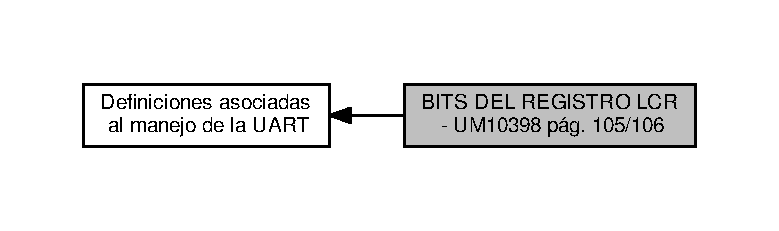
\includegraphics[width=350pt]{group___l_c_r_b_i_t_s}
\end{center}
\end{figure}
\subsection*{Macros}
\begin{DoxyCompactItemize}
\item 
\#define \hyperlink{group___l_c_r_b_i_t_s_ga81ce767ec824bfc681ba09c07f5fa7f8}{U0\+L\+C\+R\+\_\+\+W\+O\+R\+D\+\_\+\+L\+E\+N\+G\+T\+H\+\_\+\+S\+E\+L\+E\+C\+T\+\_\+5\+B\+IT}~(0x00 $<$$<$ 0)
\begin{DoxyCompactList}\small\item\em Largo de la palabra transmitida \+: 5 bits. \end{DoxyCompactList}\item 
\#define \hyperlink{group___l_c_r_b_i_t_s_ga22fa185de67e4fe6f1ee0f6c33d350f6}{U0\+L\+C\+R\+\_\+\+W\+O\+R\+D\+\_\+\+L\+E\+N\+G\+T\+H\+\_\+\+S\+E\+L\+E\+C\+T\+\_\+6\+B\+IT}~(0x01 $<$$<$ 0)
\begin{DoxyCompactList}\small\item\em Largo de la palabra transmitida \+: 6 bits. \end{DoxyCompactList}\item 
\#define \hyperlink{group___l_c_r_b_i_t_s_ga2f83575d55d06ad71aa8e0acaa8c7c05}{U0\+L\+C\+R\+\_\+\+W\+O\+R\+D\+\_\+\+L\+E\+N\+G\+T\+H\+\_\+\+S\+E\+L\+E\+C\+T\+\_\+7\+B\+IT}~(0x02 $<$$<$ 0)
\begin{DoxyCompactList}\small\item\em Largo de la palabra transmitida \+: 7 bits. \end{DoxyCompactList}\item 
\#define \hyperlink{group___l_c_r_b_i_t_s_gaec263e29a2f840e2a99c3aab0b244cf1}{U0\+L\+C\+R\+\_\+\+W\+O\+R\+D\+\_\+\+L\+E\+N\+G\+T\+H\+\_\+\+S\+E\+L\+E\+C\+T\+\_\+8\+B\+IT}~(0x03 $<$$<$ 0)
\begin{DoxyCompactList}\small\item\em Largo de la palabra transmitida \+: 8 bits. \end{DoxyCompactList}\item 
\#define \hyperlink{group___l_c_r_b_i_t_s_gadb93dcea13ecddc341bf08bcbcfd5710}{U0\+L\+C\+R\+\_\+\+S\+T\+O\+P\+\_\+\+B\+I\+T\+\_\+\+S\+E\+L\+E\+C\+T\+\_\+1\+B\+IT}~(0x00 $<$$<$ 2)
\begin{DoxyCompactList}\small\item\em Selecciono 1 bits de stop. Es un cero por default. \end{DoxyCompactList}\item 
\#define \hyperlink{group___l_c_r_b_i_t_s_ga2759f7645aa800c7685a05c10d0117aa}{U0\+L\+C\+R\+\_\+\+S\+T\+O\+P\+\_\+\+B\+I\+T\+\_\+\+S\+E\+L\+E\+C\+T\+\_\+2\+B\+IT}~(0x01 $<$$<$ 2)
\begin{DoxyCompactList}\small\item\em Selecciono 2 bits de stop. Sino queda un bit. \end{DoxyCompactList}\item 
\#define \hyperlink{group___l_c_r_b_i_t_s_ga7e31bc47be1ba3671357efd929e2b733}{U0\+L\+C\+R\+\_\+\+P\+A\+R\+I\+T\+Y\+\_\+\+E\+N\+A\+B\+LE}~(0x01 $<$$<$ 3)
\begin{DoxyCompactList}\small\item\em Habilita la generacion y chequeo paridad. \end{DoxyCompactList}\item 
\#define \hyperlink{group___l_c_r_b_i_t_s_ga216d11e84d54db2b62eba03dbd40a740}{U0\+L\+C\+R\+\_\+\+P\+A\+R\+I\+T\+Y\+\_\+\+S\+E\+L\+E\+C\+T\+\_\+\+O\+DD}~(0x00 $<$$<$ 4)
\begin{DoxyCompactList}\small\item\em Paridad par. \end{DoxyCompactList}\item 
\#define \hyperlink{group___l_c_r_b_i_t_s_ga01cafa504c142a81109a3a5105ba8ed5}{U0\+L\+C\+R\+\_\+\+P\+A\+R\+I\+T\+Y\+\_\+\+S\+E\+L\+E\+C\+T\+\_\+\+E\+V\+EN}~(0x01 $<$$<$ 4)
\begin{DoxyCompactList}\small\item\em Paridad impar. \end{DoxyCompactList}\item 
\#define \hyperlink{group___l_c_r_b_i_t_s_ga11f193765cc61579da49734fb03f45ae}{U0\+L\+C\+R\+\_\+\+P\+A\+R\+I\+T\+Y\+\_\+\+S\+E\+L\+E\+C\+T\+\_\+1\+S\+T\+I\+CK}~(0x02 $<$$<$ 4)
\begin{DoxyCompactList}\small\item\em Paridad 1 forzado. \end{DoxyCompactList}\item 
\#define \hyperlink{group___l_c_r_b_i_t_s_gac59a010ca333a7dab781e89bc467b3c8}{U0\+L\+C\+R\+\_\+\+P\+A\+R\+I\+T\+Y\+\_\+\+S\+E\+L\+E\+C\+T\+\_\+0\+S\+T\+I\+CK}~(0x03 $<$$<$ 4)
\begin{DoxyCompactList}\small\item\em Paridad 0 forzado. \end{DoxyCompactList}\item 
\#define \hyperlink{group___l_c_r_b_i_t_s_ga4f480d22c82a1322076a77e69c79924a}{U0\+L\+C\+R\+\_\+\+B\+R\+E\+A\+K\+\_\+\+C\+O\+N\+T\+R\+OL}~(0x01 $<$$<$ 6)
\begin{DoxyCompactList}\small\item\em Habilita Break Transmission \+: T\+XD se fuerza a cero cuando este bit se encuentra en uno. \end{DoxyCompactList}\item 
\#define \hyperlink{group___l_c_r_b_i_t_s_ga7b13c20c8707623317b4b8d452291193}{U0\+L\+C\+R\+\_\+\+D\+L\+AB}~(0x01 $<$$<$ 7)
\begin{DoxyCompactList}\small\item\em Habilita el acceso a Divisor Latches. \end{DoxyCompactList}\item 
\#define \hyperlink{group___l_c_r_b_i_t_s_ga63421105f318c07c617f31b8690d235d}{U0\+F\+C\+R\+\_\+\+F\+I\+F\+O\+\_\+\+E\+N\+A\+B\+LE}~(0x01 $<$$<$ 0)
\begin{DoxyCompactList}\small\item\em Habilita las F\+I\+FO de Tx y Rx. Al modificar este bit se limpian las F\+I\+FO. Habilita el acceso de los bits U0\+F\+CR\mbox{[}7\+:1\mbox{]}. \end{DoxyCompactList}\item 
\#define \hyperlink{group___l_c_r_b_i_t_s_ga240a3e574e516161ecce09cfdf83c5c8}{U0\+F\+C\+R\+\_\+\+R\+X\+\_\+\+F\+I\+F\+O\+\_\+\+R\+E\+S\+ET}~(0x01 $<$$<$ 1)
\begin{DoxyCompactList}\small\item\em Limpia todos los bits de la fifo Rx. \end{DoxyCompactList}\item 
\#define \hyperlink{group___l_c_r_b_i_t_s_ga6d547993f119687d90a053c8266b4e93}{U0\+F\+C\+R\+\_\+\+T\+X\+\_\+\+F\+I\+F\+O\+\_\+\+R\+E\+S\+ET}~(0x01 $<$$<$ 2)
\begin{DoxyCompactList}\small\item\em Limpia todos los bits de la fifo Tx. \end{DoxyCompactList}\item 
\#define \hyperlink{group___l_c_r_b_i_t_s_ga464b2e23a47585bf3710a5d71cf03e39}{U0\+F\+C\+R\+\_\+\+R\+X\+\_\+\+T\+R\+I\+G\+G\+E\+R\+\_\+\+L\+E\+V\+E\+L\+\_\+1}~(0x00 $<$$<$ 6)
\begin{DoxyCompactList}\small\item\em Trigger Level 0 \+: 1 caracter. \end{DoxyCompactList}\item 
\#define \hyperlink{group___l_c_r_b_i_t_s_ga3678812db1dc70d302edaa1ed75fc6de}{U0\+F\+C\+R\+\_\+\+R\+X\+\_\+\+T\+R\+I\+G\+G\+E\+R\+\_\+\+L\+E\+V\+E\+L\+\_\+2}~(0x01 $<$$<$ 6)
\begin{DoxyCompactList}\small\item\em Trigger Level 1 \+: 4 caracter. \end{DoxyCompactList}\item 
\#define \hyperlink{group___l_c_r_b_i_t_s_ga662bff8ef52bde6238fc6a2d90dc387f}{U0\+F\+C\+R\+\_\+\+R\+X\+\_\+\+T\+R\+I\+G\+G\+E\+R\+\_\+\+L\+E\+V\+E\+L\+\_\+3}~(0x02 $<$$<$ 6)
\begin{DoxyCompactList}\small\item\em Trigger Level 2 \+: 8 caracter. \end{DoxyCompactList}\item 
\#define \hyperlink{group___l_c_r_b_i_t_s_ga83db7cf080f263b776a48e29f46504d0}{U0\+F\+C\+R\+\_\+\+R\+X\+\_\+\+T\+R\+I\+G\+G\+E\+R\+\_\+\+L\+E\+V\+E\+L\+\_\+4}~(0x03 $<$$<$ 6)
\begin{DoxyCompactList}\small\item\em Trigger Level 3 \+: 16 caracter. \end{DoxyCompactList}\end{DoxyCompactItemize}


\subsection{Detailed Description}
The U0\+L\+CR determines the format of the data character that is to be transmitted or received. 

The U0\+F\+CR controls the operation of the U\+A\+RT RX and TX F\+I\+F\+Os.

\subsection{Macro Definition Documentation}
\index{B\+I\+T\+S D\+E\+L R\+E\+G\+I\+S\+T\+R\+O L\+C\+R -\/ U\+M10398 pág. 105/106@{B\+I\+T\+S D\+E\+L R\+E\+G\+I\+S\+T\+R\+O L\+C\+R -\/ U\+M10398 pág. 105/106}!U0\+F\+C\+R\+\_\+\+F\+I\+F\+O\+\_\+\+E\+N\+A\+B\+LE@{U0\+F\+C\+R\+\_\+\+F\+I\+F\+O\+\_\+\+E\+N\+A\+B\+LE}}
\index{U0\+F\+C\+R\+\_\+\+F\+I\+F\+O\+\_\+\+E\+N\+A\+B\+LE@{U0\+F\+C\+R\+\_\+\+F\+I\+F\+O\+\_\+\+E\+N\+A\+B\+LE}!B\+I\+T\+S D\+E\+L R\+E\+G\+I\+S\+T\+R\+O L\+C\+R -\/ U\+M10398 pág. 105/106@{B\+I\+T\+S D\+E\+L R\+E\+G\+I\+S\+T\+R\+O L\+C\+R -\/ U\+M10398 pág. 105/106}}
\subsubsection[{\texorpdfstring{U0\+F\+C\+R\+\_\+\+F\+I\+F\+O\+\_\+\+E\+N\+A\+B\+LE}{U0FCR_FIFO_ENABLE}}]{\setlength{\rightskip}{0pt plus 5cm}\#define U0\+F\+C\+R\+\_\+\+F\+I\+F\+O\+\_\+\+E\+N\+A\+B\+LE~(0x01 $<$$<$ 0)}\hypertarget{group___l_c_r_b_i_t_s_ga63421105f318c07c617f31b8690d235d}{}\label{group___l_c_r_b_i_t_s_ga63421105f318c07c617f31b8690d235d}


Habilita las F\+I\+FO de Tx y Rx. Al modificar este bit se limpian las F\+I\+FO. Habilita el acceso de los bits U0\+F\+CR\mbox{[}7\+:1\mbox{]}. 



Definition at line 324 of file uart.\+h.

\index{B\+I\+T\+S D\+E\+L R\+E\+G\+I\+S\+T\+R\+O L\+C\+R -\/ U\+M10398 pág. 105/106@{B\+I\+T\+S D\+E\+L R\+E\+G\+I\+S\+T\+R\+O L\+C\+R -\/ U\+M10398 pág. 105/106}!U0\+F\+C\+R\+\_\+\+R\+X\+\_\+\+F\+I\+F\+O\+\_\+\+R\+E\+S\+ET@{U0\+F\+C\+R\+\_\+\+R\+X\+\_\+\+F\+I\+F\+O\+\_\+\+R\+E\+S\+ET}}
\index{U0\+F\+C\+R\+\_\+\+R\+X\+\_\+\+F\+I\+F\+O\+\_\+\+R\+E\+S\+ET@{U0\+F\+C\+R\+\_\+\+R\+X\+\_\+\+F\+I\+F\+O\+\_\+\+R\+E\+S\+ET}!B\+I\+T\+S D\+E\+L R\+E\+G\+I\+S\+T\+R\+O L\+C\+R -\/ U\+M10398 pág. 105/106@{B\+I\+T\+S D\+E\+L R\+E\+G\+I\+S\+T\+R\+O L\+C\+R -\/ U\+M10398 pág. 105/106}}
\subsubsection[{\texorpdfstring{U0\+F\+C\+R\+\_\+\+R\+X\+\_\+\+F\+I\+F\+O\+\_\+\+R\+E\+S\+ET}{U0FCR_RX_FIFO_RESET}}]{\setlength{\rightskip}{0pt plus 5cm}\#define U0\+F\+C\+R\+\_\+\+R\+X\+\_\+\+F\+I\+F\+O\+\_\+\+R\+E\+S\+ET~(0x01 $<$$<$ 1)}\hypertarget{group___l_c_r_b_i_t_s_ga240a3e574e516161ecce09cfdf83c5c8}{}\label{group___l_c_r_b_i_t_s_ga240a3e574e516161ecce09cfdf83c5c8}


Limpia todos los bits de la fifo Rx. 



Definition at line 326 of file uart.\+h.

\index{B\+I\+T\+S D\+E\+L R\+E\+G\+I\+S\+T\+R\+O L\+C\+R -\/ U\+M10398 pág. 105/106@{B\+I\+T\+S D\+E\+L R\+E\+G\+I\+S\+T\+R\+O L\+C\+R -\/ U\+M10398 pág. 105/106}!U0\+F\+C\+R\+\_\+\+R\+X\+\_\+\+T\+R\+I\+G\+G\+E\+R\+\_\+\+L\+E\+V\+E\+L\+\_\+1@{U0\+F\+C\+R\+\_\+\+R\+X\+\_\+\+T\+R\+I\+G\+G\+E\+R\+\_\+\+L\+E\+V\+E\+L\+\_\+1}}
\index{U0\+F\+C\+R\+\_\+\+R\+X\+\_\+\+T\+R\+I\+G\+G\+E\+R\+\_\+\+L\+E\+V\+E\+L\+\_\+1@{U0\+F\+C\+R\+\_\+\+R\+X\+\_\+\+T\+R\+I\+G\+G\+E\+R\+\_\+\+L\+E\+V\+E\+L\+\_\+1}!B\+I\+T\+S D\+E\+L R\+E\+G\+I\+S\+T\+R\+O L\+C\+R -\/ U\+M10398 pág. 105/106@{B\+I\+T\+S D\+E\+L R\+E\+G\+I\+S\+T\+R\+O L\+C\+R -\/ U\+M10398 pág. 105/106}}
\subsubsection[{\texorpdfstring{U0\+F\+C\+R\+\_\+\+R\+X\+\_\+\+T\+R\+I\+G\+G\+E\+R\+\_\+\+L\+E\+V\+E\+L\+\_\+1}{U0FCR_RX_TRIGGER_LEVEL_1}}]{\setlength{\rightskip}{0pt plus 5cm}\#define U0\+F\+C\+R\+\_\+\+R\+X\+\_\+\+T\+R\+I\+G\+G\+E\+R\+\_\+\+L\+E\+V\+E\+L\+\_\+1~(0x00 $<$$<$ 6)}\hypertarget{group___l_c_r_b_i_t_s_ga464b2e23a47585bf3710a5d71cf03e39}{}\label{group___l_c_r_b_i_t_s_ga464b2e23a47585bf3710a5d71cf03e39}


Trigger Level 0 \+: 1 caracter. 



Definition at line 331 of file uart.\+h.

\index{B\+I\+T\+S D\+E\+L R\+E\+G\+I\+S\+T\+R\+O L\+C\+R -\/ U\+M10398 pág. 105/106@{B\+I\+T\+S D\+E\+L R\+E\+G\+I\+S\+T\+R\+O L\+C\+R -\/ U\+M10398 pág. 105/106}!U0\+F\+C\+R\+\_\+\+R\+X\+\_\+\+T\+R\+I\+G\+G\+E\+R\+\_\+\+L\+E\+V\+E\+L\+\_\+2@{U0\+F\+C\+R\+\_\+\+R\+X\+\_\+\+T\+R\+I\+G\+G\+E\+R\+\_\+\+L\+E\+V\+E\+L\+\_\+2}}
\index{U0\+F\+C\+R\+\_\+\+R\+X\+\_\+\+T\+R\+I\+G\+G\+E\+R\+\_\+\+L\+E\+V\+E\+L\+\_\+2@{U0\+F\+C\+R\+\_\+\+R\+X\+\_\+\+T\+R\+I\+G\+G\+E\+R\+\_\+\+L\+E\+V\+E\+L\+\_\+2}!B\+I\+T\+S D\+E\+L R\+E\+G\+I\+S\+T\+R\+O L\+C\+R -\/ U\+M10398 pág. 105/106@{B\+I\+T\+S D\+E\+L R\+E\+G\+I\+S\+T\+R\+O L\+C\+R -\/ U\+M10398 pág. 105/106}}
\subsubsection[{\texorpdfstring{U0\+F\+C\+R\+\_\+\+R\+X\+\_\+\+T\+R\+I\+G\+G\+E\+R\+\_\+\+L\+E\+V\+E\+L\+\_\+2}{U0FCR_RX_TRIGGER_LEVEL_2}}]{\setlength{\rightskip}{0pt plus 5cm}\#define U0\+F\+C\+R\+\_\+\+R\+X\+\_\+\+T\+R\+I\+G\+G\+E\+R\+\_\+\+L\+E\+V\+E\+L\+\_\+2~(0x01 $<$$<$ 6)}\hypertarget{group___l_c_r_b_i_t_s_ga3678812db1dc70d302edaa1ed75fc6de}{}\label{group___l_c_r_b_i_t_s_ga3678812db1dc70d302edaa1ed75fc6de}


Trigger Level 1 \+: 4 caracter. 



Definition at line 333 of file uart.\+h.

\index{B\+I\+T\+S D\+E\+L R\+E\+G\+I\+S\+T\+R\+O L\+C\+R -\/ U\+M10398 pág. 105/106@{B\+I\+T\+S D\+E\+L R\+E\+G\+I\+S\+T\+R\+O L\+C\+R -\/ U\+M10398 pág. 105/106}!U0\+F\+C\+R\+\_\+\+R\+X\+\_\+\+T\+R\+I\+G\+G\+E\+R\+\_\+\+L\+E\+V\+E\+L\+\_\+3@{U0\+F\+C\+R\+\_\+\+R\+X\+\_\+\+T\+R\+I\+G\+G\+E\+R\+\_\+\+L\+E\+V\+E\+L\+\_\+3}}
\index{U0\+F\+C\+R\+\_\+\+R\+X\+\_\+\+T\+R\+I\+G\+G\+E\+R\+\_\+\+L\+E\+V\+E\+L\+\_\+3@{U0\+F\+C\+R\+\_\+\+R\+X\+\_\+\+T\+R\+I\+G\+G\+E\+R\+\_\+\+L\+E\+V\+E\+L\+\_\+3}!B\+I\+T\+S D\+E\+L R\+E\+G\+I\+S\+T\+R\+O L\+C\+R -\/ U\+M10398 pág. 105/106@{B\+I\+T\+S D\+E\+L R\+E\+G\+I\+S\+T\+R\+O L\+C\+R -\/ U\+M10398 pág. 105/106}}
\subsubsection[{\texorpdfstring{U0\+F\+C\+R\+\_\+\+R\+X\+\_\+\+T\+R\+I\+G\+G\+E\+R\+\_\+\+L\+E\+V\+E\+L\+\_\+3}{U0FCR_RX_TRIGGER_LEVEL_3}}]{\setlength{\rightskip}{0pt plus 5cm}\#define U0\+F\+C\+R\+\_\+\+R\+X\+\_\+\+T\+R\+I\+G\+G\+E\+R\+\_\+\+L\+E\+V\+E\+L\+\_\+3~(0x02 $<$$<$ 6)}\hypertarget{group___l_c_r_b_i_t_s_ga662bff8ef52bde6238fc6a2d90dc387f}{}\label{group___l_c_r_b_i_t_s_ga662bff8ef52bde6238fc6a2d90dc387f}


Trigger Level 2 \+: 8 caracter. 



Definition at line 335 of file uart.\+h.

\index{B\+I\+T\+S D\+E\+L R\+E\+G\+I\+S\+T\+R\+O L\+C\+R -\/ U\+M10398 pág. 105/106@{B\+I\+T\+S D\+E\+L R\+E\+G\+I\+S\+T\+R\+O L\+C\+R -\/ U\+M10398 pág. 105/106}!U0\+F\+C\+R\+\_\+\+R\+X\+\_\+\+T\+R\+I\+G\+G\+E\+R\+\_\+\+L\+E\+V\+E\+L\+\_\+4@{U0\+F\+C\+R\+\_\+\+R\+X\+\_\+\+T\+R\+I\+G\+G\+E\+R\+\_\+\+L\+E\+V\+E\+L\+\_\+4}}
\index{U0\+F\+C\+R\+\_\+\+R\+X\+\_\+\+T\+R\+I\+G\+G\+E\+R\+\_\+\+L\+E\+V\+E\+L\+\_\+4@{U0\+F\+C\+R\+\_\+\+R\+X\+\_\+\+T\+R\+I\+G\+G\+E\+R\+\_\+\+L\+E\+V\+E\+L\+\_\+4}!B\+I\+T\+S D\+E\+L R\+E\+G\+I\+S\+T\+R\+O L\+C\+R -\/ U\+M10398 pág. 105/106@{B\+I\+T\+S D\+E\+L R\+E\+G\+I\+S\+T\+R\+O L\+C\+R -\/ U\+M10398 pág. 105/106}}
\subsubsection[{\texorpdfstring{U0\+F\+C\+R\+\_\+\+R\+X\+\_\+\+T\+R\+I\+G\+G\+E\+R\+\_\+\+L\+E\+V\+E\+L\+\_\+4}{U0FCR_RX_TRIGGER_LEVEL_4}}]{\setlength{\rightskip}{0pt plus 5cm}\#define U0\+F\+C\+R\+\_\+\+R\+X\+\_\+\+T\+R\+I\+G\+G\+E\+R\+\_\+\+L\+E\+V\+E\+L\+\_\+4~(0x03 $<$$<$ 6)}\hypertarget{group___l_c_r_b_i_t_s_ga83db7cf080f263b776a48e29f46504d0}{}\label{group___l_c_r_b_i_t_s_ga83db7cf080f263b776a48e29f46504d0}


Trigger Level 3 \+: 16 caracter. 



Definition at line 337 of file uart.\+h.

\index{B\+I\+T\+S D\+E\+L R\+E\+G\+I\+S\+T\+R\+O L\+C\+R -\/ U\+M10398 pág. 105/106@{B\+I\+T\+S D\+E\+L R\+E\+G\+I\+S\+T\+R\+O L\+C\+R -\/ U\+M10398 pág. 105/106}!U0\+F\+C\+R\+\_\+\+T\+X\+\_\+\+F\+I\+F\+O\+\_\+\+R\+E\+S\+ET@{U0\+F\+C\+R\+\_\+\+T\+X\+\_\+\+F\+I\+F\+O\+\_\+\+R\+E\+S\+ET}}
\index{U0\+F\+C\+R\+\_\+\+T\+X\+\_\+\+F\+I\+F\+O\+\_\+\+R\+E\+S\+ET@{U0\+F\+C\+R\+\_\+\+T\+X\+\_\+\+F\+I\+F\+O\+\_\+\+R\+E\+S\+ET}!B\+I\+T\+S D\+E\+L R\+E\+G\+I\+S\+T\+R\+O L\+C\+R -\/ U\+M10398 pág. 105/106@{B\+I\+T\+S D\+E\+L R\+E\+G\+I\+S\+T\+R\+O L\+C\+R -\/ U\+M10398 pág. 105/106}}
\subsubsection[{\texorpdfstring{U0\+F\+C\+R\+\_\+\+T\+X\+\_\+\+F\+I\+F\+O\+\_\+\+R\+E\+S\+ET}{U0FCR_TX_FIFO_RESET}}]{\setlength{\rightskip}{0pt plus 5cm}\#define U0\+F\+C\+R\+\_\+\+T\+X\+\_\+\+F\+I\+F\+O\+\_\+\+R\+E\+S\+ET~(0x01 $<$$<$ 2)}\hypertarget{group___l_c_r_b_i_t_s_ga6d547993f119687d90a053c8266b4e93}{}\label{group___l_c_r_b_i_t_s_ga6d547993f119687d90a053c8266b4e93}


Limpia todos los bits de la fifo Tx. 



Definition at line 328 of file uart.\+h.

\index{B\+I\+T\+S D\+E\+L R\+E\+G\+I\+S\+T\+R\+O L\+C\+R -\/ U\+M10398 pág. 105/106@{B\+I\+T\+S D\+E\+L R\+E\+G\+I\+S\+T\+R\+O L\+C\+R -\/ U\+M10398 pág. 105/106}!U0\+L\+C\+R\+\_\+\+B\+R\+E\+A\+K\+\_\+\+C\+O\+N\+T\+R\+OL@{U0\+L\+C\+R\+\_\+\+B\+R\+E\+A\+K\+\_\+\+C\+O\+N\+T\+R\+OL}}
\index{U0\+L\+C\+R\+\_\+\+B\+R\+E\+A\+K\+\_\+\+C\+O\+N\+T\+R\+OL@{U0\+L\+C\+R\+\_\+\+B\+R\+E\+A\+K\+\_\+\+C\+O\+N\+T\+R\+OL}!B\+I\+T\+S D\+E\+L R\+E\+G\+I\+S\+T\+R\+O L\+C\+R -\/ U\+M10398 pág. 105/106@{B\+I\+T\+S D\+E\+L R\+E\+G\+I\+S\+T\+R\+O L\+C\+R -\/ U\+M10398 pág. 105/106}}
\subsubsection[{\texorpdfstring{U0\+L\+C\+R\+\_\+\+B\+R\+E\+A\+K\+\_\+\+C\+O\+N\+T\+R\+OL}{U0LCR_BREAK_CONTROL}}]{\setlength{\rightskip}{0pt plus 5cm}\#define U0\+L\+C\+R\+\_\+\+B\+R\+E\+A\+K\+\_\+\+C\+O\+N\+T\+R\+OL~(0x01 $<$$<$ 6)}\hypertarget{group___l_c_r_b_i_t_s_ga4f480d22c82a1322076a77e69c79924a}{}\label{group___l_c_r_b_i_t_s_ga4f480d22c82a1322076a77e69c79924a}


Habilita Break Transmission \+: T\+XD se fuerza a cero cuando este bit se encuentra en uno. 



Definition at line 307 of file uart.\+h.

\index{B\+I\+T\+S D\+E\+L R\+E\+G\+I\+S\+T\+R\+O L\+C\+R -\/ U\+M10398 pág. 105/106@{B\+I\+T\+S D\+E\+L R\+E\+G\+I\+S\+T\+R\+O L\+C\+R -\/ U\+M10398 pág. 105/106}!U0\+L\+C\+R\+\_\+\+D\+L\+AB@{U0\+L\+C\+R\+\_\+\+D\+L\+AB}}
\index{U0\+L\+C\+R\+\_\+\+D\+L\+AB@{U0\+L\+C\+R\+\_\+\+D\+L\+AB}!B\+I\+T\+S D\+E\+L R\+E\+G\+I\+S\+T\+R\+O L\+C\+R -\/ U\+M10398 pág. 105/106@{B\+I\+T\+S D\+E\+L R\+E\+G\+I\+S\+T\+R\+O L\+C\+R -\/ U\+M10398 pág. 105/106}}
\subsubsection[{\texorpdfstring{U0\+L\+C\+R\+\_\+\+D\+L\+AB}{U0LCR_DLAB}}]{\setlength{\rightskip}{0pt plus 5cm}\#define U0\+L\+C\+R\+\_\+\+D\+L\+AB~(0x01 $<$$<$ 7)}\hypertarget{group___l_c_r_b_i_t_s_ga7b13c20c8707623317b4b8d452291193}{}\label{group___l_c_r_b_i_t_s_ga7b13c20c8707623317b4b8d452291193}


Habilita el acceso a Divisor Latches. 



Definition at line 309 of file uart.\+h.

\index{B\+I\+T\+S D\+E\+L R\+E\+G\+I\+S\+T\+R\+O L\+C\+R -\/ U\+M10398 pág. 105/106@{B\+I\+T\+S D\+E\+L R\+E\+G\+I\+S\+T\+R\+O L\+C\+R -\/ U\+M10398 pág. 105/106}!U0\+L\+C\+R\+\_\+\+P\+A\+R\+I\+T\+Y\+\_\+\+E\+N\+A\+B\+LE@{U0\+L\+C\+R\+\_\+\+P\+A\+R\+I\+T\+Y\+\_\+\+E\+N\+A\+B\+LE}}
\index{U0\+L\+C\+R\+\_\+\+P\+A\+R\+I\+T\+Y\+\_\+\+E\+N\+A\+B\+LE@{U0\+L\+C\+R\+\_\+\+P\+A\+R\+I\+T\+Y\+\_\+\+E\+N\+A\+B\+LE}!B\+I\+T\+S D\+E\+L R\+E\+G\+I\+S\+T\+R\+O L\+C\+R -\/ U\+M10398 pág. 105/106@{B\+I\+T\+S D\+E\+L R\+E\+G\+I\+S\+T\+R\+O L\+C\+R -\/ U\+M10398 pág. 105/106}}
\subsubsection[{\texorpdfstring{U0\+L\+C\+R\+\_\+\+P\+A\+R\+I\+T\+Y\+\_\+\+E\+N\+A\+B\+LE}{U0LCR_PARITY_ENABLE}}]{\setlength{\rightskip}{0pt plus 5cm}\#define U0\+L\+C\+R\+\_\+\+P\+A\+R\+I\+T\+Y\+\_\+\+E\+N\+A\+B\+LE~(0x01 $<$$<$ 3)}\hypertarget{group___l_c_r_b_i_t_s_ga7e31bc47be1ba3671357efd929e2b733}{}\label{group___l_c_r_b_i_t_s_ga7e31bc47be1ba3671357efd929e2b733}


Habilita la generacion y chequeo paridad. 



Definition at line 295 of file uart.\+h.

\index{B\+I\+T\+S D\+E\+L R\+E\+G\+I\+S\+T\+R\+O L\+C\+R -\/ U\+M10398 pág. 105/106@{B\+I\+T\+S D\+E\+L R\+E\+G\+I\+S\+T\+R\+O L\+C\+R -\/ U\+M10398 pág. 105/106}!U0\+L\+C\+R\+\_\+\+P\+A\+R\+I\+T\+Y\+\_\+\+S\+E\+L\+E\+C\+T\+\_\+0\+S\+T\+I\+CK@{U0\+L\+C\+R\+\_\+\+P\+A\+R\+I\+T\+Y\+\_\+\+S\+E\+L\+E\+C\+T\+\_\+0\+S\+T\+I\+CK}}
\index{U0\+L\+C\+R\+\_\+\+P\+A\+R\+I\+T\+Y\+\_\+\+S\+E\+L\+E\+C\+T\+\_\+0\+S\+T\+I\+CK@{U0\+L\+C\+R\+\_\+\+P\+A\+R\+I\+T\+Y\+\_\+\+S\+E\+L\+E\+C\+T\+\_\+0\+S\+T\+I\+CK}!B\+I\+T\+S D\+E\+L R\+E\+G\+I\+S\+T\+R\+O L\+C\+R -\/ U\+M10398 pág. 105/106@{B\+I\+T\+S D\+E\+L R\+E\+G\+I\+S\+T\+R\+O L\+C\+R -\/ U\+M10398 pág. 105/106}}
\subsubsection[{\texorpdfstring{U0\+L\+C\+R\+\_\+\+P\+A\+R\+I\+T\+Y\+\_\+\+S\+E\+L\+E\+C\+T\+\_\+0\+S\+T\+I\+CK}{U0LCR_PARITY_SELECT_0STICK}}]{\setlength{\rightskip}{0pt plus 5cm}\#define U0\+L\+C\+R\+\_\+\+P\+A\+R\+I\+T\+Y\+\_\+\+S\+E\+L\+E\+C\+T\+\_\+0\+S\+T\+I\+CK~(0x03 $<$$<$ 4)}\hypertarget{group___l_c_r_b_i_t_s_gac59a010ca333a7dab781e89bc467b3c8}{}\label{group___l_c_r_b_i_t_s_gac59a010ca333a7dab781e89bc467b3c8}


Paridad 0 forzado. 



Definition at line 304 of file uart.\+h.

\index{B\+I\+T\+S D\+E\+L R\+E\+G\+I\+S\+T\+R\+O L\+C\+R -\/ U\+M10398 pág. 105/106@{B\+I\+T\+S D\+E\+L R\+E\+G\+I\+S\+T\+R\+O L\+C\+R -\/ U\+M10398 pág. 105/106}!U0\+L\+C\+R\+\_\+\+P\+A\+R\+I\+T\+Y\+\_\+\+S\+E\+L\+E\+C\+T\+\_\+1\+S\+T\+I\+CK@{U0\+L\+C\+R\+\_\+\+P\+A\+R\+I\+T\+Y\+\_\+\+S\+E\+L\+E\+C\+T\+\_\+1\+S\+T\+I\+CK}}
\index{U0\+L\+C\+R\+\_\+\+P\+A\+R\+I\+T\+Y\+\_\+\+S\+E\+L\+E\+C\+T\+\_\+1\+S\+T\+I\+CK@{U0\+L\+C\+R\+\_\+\+P\+A\+R\+I\+T\+Y\+\_\+\+S\+E\+L\+E\+C\+T\+\_\+1\+S\+T\+I\+CK}!B\+I\+T\+S D\+E\+L R\+E\+G\+I\+S\+T\+R\+O L\+C\+R -\/ U\+M10398 pág. 105/106@{B\+I\+T\+S D\+E\+L R\+E\+G\+I\+S\+T\+R\+O L\+C\+R -\/ U\+M10398 pág. 105/106}}
\subsubsection[{\texorpdfstring{U0\+L\+C\+R\+\_\+\+P\+A\+R\+I\+T\+Y\+\_\+\+S\+E\+L\+E\+C\+T\+\_\+1\+S\+T\+I\+CK}{U0LCR_PARITY_SELECT_1STICK}}]{\setlength{\rightskip}{0pt plus 5cm}\#define U0\+L\+C\+R\+\_\+\+P\+A\+R\+I\+T\+Y\+\_\+\+S\+E\+L\+E\+C\+T\+\_\+1\+S\+T\+I\+CK~(0x02 $<$$<$ 4)}\hypertarget{group___l_c_r_b_i_t_s_ga11f193765cc61579da49734fb03f45ae}{}\label{group___l_c_r_b_i_t_s_ga11f193765cc61579da49734fb03f45ae}


Paridad 1 forzado. 



Definition at line 302 of file uart.\+h.

\index{B\+I\+T\+S D\+E\+L R\+E\+G\+I\+S\+T\+R\+O L\+C\+R -\/ U\+M10398 pág. 105/106@{B\+I\+T\+S D\+E\+L R\+E\+G\+I\+S\+T\+R\+O L\+C\+R -\/ U\+M10398 pág. 105/106}!U0\+L\+C\+R\+\_\+\+P\+A\+R\+I\+T\+Y\+\_\+\+S\+E\+L\+E\+C\+T\+\_\+\+E\+V\+EN@{U0\+L\+C\+R\+\_\+\+P\+A\+R\+I\+T\+Y\+\_\+\+S\+E\+L\+E\+C\+T\+\_\+\+E\+V\+EN}}
\index{U0\+L\+C\+R\+\_\+\+P\+A\+R\+I\+T\+Y\+\_\+\+S\+E\+L\+E\+C\+T\+\_\+\+E\+V\+EN@{U0\+L\+C\+R\+\_\+\+P\+A\+R\+I\+T\+Y\+\_\+\+S\+E\+L\+E\+C\+T\+\_\+\+E\+V\+EN}!B\+I\+T\+S D\+E\+L R\+E\+G\+I\+S\+T\+R\+O L\+C\+R -\/ U\+M10398 pág. 105/106@{B\+I\+T\+S D\+E\+L R\+E\+G\+I\+S\+T\+R\+O L\+C\+R -\/ U\+M10398 pág. 105/106}}
\subsubsection[{\texorpdfstring{U0\+L\+C\+R\+\_\+\+P\+A\+R\+I\+T\+Y\+\_\+\+S\+E\+L\+E\+C\+T\+\_\+\+E\+V\+EN}{U0LCR_PARITY_SELECT_EVEN}}]{\setlength{\rightskip}{0pt plus 5cm}\#define U0\+L\+C\+R\+\_\+\+P\+A\+R\+I\+T\+Y\+\_\+\+S\+E\+L\+E\+C\+T\+\_\+\+E\+V\+EN~(0x01 $<$$<$ 4)}\hypertarget{group___l_c_r_b_i_t_s_ga01cafa504c142a81109a3a5105ba8ed5}{}\label{group___l_c_r_b_i_t_s_ga01cafa504c142a81109a3a5105ba8ed5}


Paridad impar. 



Definition at line 300 of file uart.\+h.

\index{B\+I\+T\+S D\+E\+L R\+E\+G\+I\+S\+T\+R\+O L\+C\+R -\/ U\+M10398 pág. 105/106@{B\+I\+T\+S D\+E\+L R\+E\+G\+I\+S\+T\+R\+O L\+C\+R -\/ U\+M10398 pág. 105/106}!U0\+L\+C\+R\+\_\+\+P\+A\+R\+I\+T\+Y\+\_\+\+S\+E\+L\+E\+C\+T\+\_\+\+O\+DD@{U0\+L\+C\+R\+\_\+\+P\+A\+R\+I\+T\+Y\+\_\+\+S\+E\+L\+E\+C\+T\+\_\+\+O\+DD}}
\index{U0\+L\+C\+R\+\_\+\+P\+A\+R\+I\+T\+Y\+\_\+\+S\+E\+L\+E\+C\+T\+\_\+\+O\+DD@{U0\+L\+C\+R\+\_\+\+P\+A\+R\+I\+T\+Y\+\_\+\+S\+E\+L\+E\+C\+T\+\_\+\+O\+DD}!B\+I\+T\+S D\+E\+L R\+E\+G\+I\+S\+T\+R\+O L\+C\+R -\/ U\+M10398 pág. 105/106@{B\+I\+T\+S D\+E\+L R\+E\+G\+I\+S\+T\+R\+O L\+C\+R -\/ U\+M10398 pág. 105/106}}
\subsubsection[{\texorpdfstring{U0\+L\+C\+R\+\_\+\+P\+A\+R\+I\+T\+Y\+\_\+\+S\+E\+L\+E\+C\+T\+\_\+\+O\+DD}{U0LCR_PARITY_SELECT_ODD}}]{\setlength{\rightskip}{0pt plus 5cm}\#define U0\+L\+C\+R\+\_\+\+P\+A\+R\+I\+T\+Y\+\_\+\+S\+E\+L\+E\+C\+T\+\_\+\+O\+DD~(0x00 $<$$<$ 4)}\hypertarget{group___l_c_r_b_i_t_s_ga216d11e84d54db2b62eba03dbd40a740}{}\label{group___l_c_r_b_i_t_s_ga216d11e84d54db2b62eba03dbd40a740}


Paridad par. 



Definition at line 298 of file uart.\+h.

\index{B\+I\+T\+S D\+E\+L R\+E\+G\+I\+S\+T\+R\+O L\+C\+R -\/ U\+M10398 pág. 105/106@{B\+I\+T\+S D\+E\+L R\+E\+G\+I\+S\+T\+R\+O L\+C\+R -\/ U\+M10398 pág. 105/106}!U0\+L\+C\+R\+\_\+\+S\+T\+O\+P\+\_\+\+B\+I\+T\+\_\+\+S\+E\+L\+E\+C\+T\+\_\+1\+B\+IT@{U0\+L\+C\+R\+\_\+\+S\+T\+O\+P\+\_\+\+B\+I\+T\+\_\+\+S\+E\+L\+E\+C\+T\+\_\+1\+B\+IT}}
\index{U0\+L\+C\+R\+\_\+\+S\+T\+O\+P\+\_\+\+B\+I\+T\+\_\+\+S\+E\+L\+E\+C\+T\+\_\+1\+B\+IT@{U0\+L\+C\+R\+\_\+\+S\+T\+O\+P\+\_\+\+B\+I\+T\+\_\+\+S\+E\+L\+E\+C\+T\+\_\+1\+B\+IT}!B\+I\+T\+S D\+E\+L R\+E\+G\+I\+S\+T\+R\+O L\+C\+R -\/ U\+M10398 pág. 105/106@{B\+I\+T\+S D\+E\+L R\+E\+G\+I\+S\+T\+R\+O L\+C\+R -\/ U\+M10398 pág. 105/106}}
\subsubsection[{\texorpdfstring{U0\+L\+C\+R\+\_\+\+S\+T\+O\+P\+\_\+\+B\+I\+T\+\_\+\+S\+E\+L\+E\+C\+T\+\_\+1\+B\+IT}{U0LCR_STOP_BIT_SELECT_1BIT}}]{\setlength{\rightskip}{0pt plus 5cm}\#define U0\+L\+C\+R\+\_\+\+S\+T\+O\+P\+\_\+\+B\+I\+T\+\_\+\+S\+E\+L\+E\+C\+T\+\_\+1\+B\+IT~(0x00 $<$$<$ 2)}\hypertarget{group___l_c_r_b_i_t_s_gadb93dcea13ecddc341bf08bcbcfd5710}{}\label{group___l_c_r_b_i_t_s_gadb93dcea13ecddc341bf08bcbcfd5710}


Selecciono 1 bits de stop. Es un cero por default. 



Definition at line 291 of file uart.\+h.

\index{B\+I\+T\+S D\+E\+L R\+E\+G\+I\+S\+T\+R\+O L\+C\+R -\/ U\+M10398 pág. 105/106@{B\+I\+T\+S D\+E\+L R\+E\+G\+I\+S\+T\+R\+O L\+C\+R -\/ U\+M10398 pág. 105/106}!U0\+L\+C\+R\+\_\+\+S\+T\+O\+P\+\_\+\+B\+I\+T\+\_\+\+S\+E\+L\+E\+C\+T\+\_\+2\+B\+IT@{U0\+L\+C\+R\+\_\+\+S\+T\+O\+P\+\_\+\+B\+I\+T\+\_\+\+S\+E\+L\+E\+C\+T\+\_\+2\+B\+IT}}
\index{U0\+L\+C\+R\+\_\+\+S\+T\+O\+P\+\_\+\+B\+I\+T\+\_\+\+S\+E\+L\+E\+C\+T\+\_\+2\+B\+IT@{U0\+L\+C\+R\+\_\+\+S\+T\+O\+P\+\_\+\+B\+I\+T\+\_\+\+S\+E\+L\+E\+C\+T\+\_\+2\+B\+IT}!B\+I\+T\+S D\+E\+L R\+E\+G\+I\+S\+T\+R\+O L\+C\+R -\/ U\+M10398 pág. 105/106@{B\+I\+T\+S D\+E\+L R\+E\+G\+I\+S\+T\+R\+O L\+C\+R -\/ U\+M10398 pág. 105/106}}
\subsubsection[{\texorpdfstring{U0\+L\+C\+R\+\_\+\+S\+T\+O\+P\+\_\+\+B\+I\+T\+\_\+\+S\+E\+L\+E\+C\+T\+\_\+2\+B\+IT}{U0LCR_STOP_BIT_SELECT_2BIT}}]{\setlength{\rightskip}{0pt plus 5cm}\#define U0\+L\+C\+R\+\_\+\+S\+T\+O\+P\+\_\+\+B\+I\+T\+\_\+\+S\+E\+L\+E\+C\+T\+\_\+2\+B\+IT~(0x01 $<$$<$ 2)}\hypertarget{group___l_c_r_b_i_t_s_ga2759f7645aa800c7685a05c10d0117aa}{}\label{group___l_c_r_b_i_t_s_ga2759f7645aa800c7685a05c10d0117aa}


Selecciono 2 bits de stop. Sino queda un bit. 



Definition at line 293 of file uart.\+h.

\index{B\+I\+T\+S D\+E\+L R\+E\+G\+I\+S\+T\+R\+O L\+C\+R -\/ U\+M10398 pág. 105/106@{B\+I\+T\+S D\+E\+L R\+E\+G\+I\+S\+T\+R\+O L\+C\+R -\/ U\+M10398 pág. 105/106}!U0\+L\+C\+R\+\_\+\+W\+O\+R\+D\+\_\+\+L\+E\+N\+G\+T\+H\+\_\+\+S\+E\+L\+E\+C\+T\+\_\+5\+B\+IT@{U0\+L\+C\+R\+\_\+\+W\+O\+R\+D\+\_\+\+L\+E\+N\+G\+T\+H\+\_\+\+S\+E\+L\+E\+C\+T\+\_\+5\+B\+IT}}
\index{U0\+L\+C\+R\+\_\+\+W\+O\+R\+D\+\_\+\+L\+E\+N\+G\+T\+H\+\_\+\+S\+E\+L\+E\+C\+T\+\_\+5\+B\+IT@{U0\+L\+C\+R\+\_\+\+W\+O\+R\+D\+\_\+\+L\+E\+N\+G\+T\+H\+\_\+\+S\+E\+L\+E\+C\+T\+\_\+5\+B\+IT}!B\+I\+T\+S D\+E\+L R\+E\+G\+I\+S\+T\+R\+O L\+C\+R -\/ U\+M10398 pág. 105/106@{B\+I\+T\+S D\+E\+L R\+E\+G\+I\+S\+T\+R\+O L\+C\+R -\/ U\+M10398 pág. 105/106}}
\subsubsection[{\texorpdfstring{U0\+L\+C\+R\+\_\+\+W\+O\+R\+D\+\_\+\+L\+E\+N\+G\+T\+H\+\_\+\+S\+E\+L\+E\+C\+T\+\_\+5\+B\+IT}{U0LCR_WORD_LENGTH_SELECT_5BIT}}]{\setlength{\rightskip}{0pt plus 5cm}\#define U0\+L\+C\+R\+\_\+\+W\+O\+R\+D\+\_\+\+L\+E\+N\+G\+T\+H\+\_\+\+S\+E\+L\+E\+C\+T\+\_\+5\+B\+IT~(0x00 $<$$<$ 0)}\hypertarget{group___l_c_r_b_i_t_s_ga81ce767ec824bfc681ba09c07f5fa7f8}{}\label{group___l_c_r_b_i_t_s_ga81ce767ec824bfc681ba09c07f5fa7f8}


Largo de la palabra transmitida \+: 5 bits. 



Definition at line 282 of file uart.\+h.

\index{B\+I\+T\+S D\+E\+L R\+E\+G\+I\+S\+T\+R\+O L\+C\+R -\/ U\+M10398 pág. 105/106@{B\+I\+T\+S D\+E\+L R\+E\+G\+I\+S\+T\+R\+O L\+C\+R -\/ U\+M10398 pág. 105/106}!U0\+L\+C\+R\+\_\+\+W\+O\+R\+D\+\_\+\+L\+E\+N\+G\+T\+H\+\_\+\+S\+E\+L\+E\+C\+T\+\_\+6\+B\+IT@{U0\+L\+C\+R\+\_\+\+W\+O\+R\+D\+\_\+\+L\+E\+N\+G\+T\+H\+\_\+\+S\+E\+L\+E\+C\+T\+\_\+6\+B\+IT}}
\index{U0\+L\+C\+R\+\_\+\+W\+O\+R\+D\+\_\+\+L\+E\+N\+G\+T\+H\+\_\+\+S\+E\+L\+E\+C\+T\+\_\+6\+B\+IT@{U0\+L\+C\+R\+\_\+\+W\+O\+R\+D\+\_\+\+L\+E\+N\+G\+T\+H\+\_\+\+S\+E\+L\+E\+C\+T\+\_\+6\+B\+IT}!B\+I\+T\+S D\+E\+L R\+E\+G\+I\+S\+T\+R\+O L\+C\+R -\/ U\+M10398 pág. 105/106@{B\+I\+T\+S D\+E\+L R\+E\+G\+I\+S\+T\+R\+O L\+C\+R -\/ U\+M10398 pág. 105/106}}
\subsubsection[{\texorpdfstring{U0\+L\+C\+R\+\_\+\+W\+O\+R\+D\+\_\+\+L\+E\+N\+G\+T\+H\+\_\+\+S\+E\+L\+E\+C\+T\+\_\+6\+B\+IT}{U0LCR_WORD_LENGTH_SELECT_6BIT}}]{\setlength{\rightskip}{0pt plus 5cm}\#define U0\+L\+C\+R\+\_\+\+W\+O\+R\+D\+\_\+\+L\+E\+N\+G\+T\+H\+\_\+\+S\+E\+L\+E\+C\+T\+\_\+6\+B\+IT~(0x01 $<$$<$ 0)}\hypertarget{group___l_c_r_b_i_t_s_ga22fa185de67e4fe6f1ee0f6c33d350f6}{}\label{group___l_c_r_b_i_t_s_ga22fa185de67e4fe6f1ee0f6c33d350f6}


Largo de la palabra transmitida \+: 6 bits. 



Definition at line 284 of file uart.\+h.

\index{B\+I\+T\+S D\+E\+L R\+E\+G\+I\+S\+T\+R\+O L\+C\+R -\/ U\+M10398 pág. 105/106@{B\+I\+T\+S D\+E\+L R\+E\+G\+I\+S\+T\+R\+O L\+C\+R -\/ U\+M10398 pág. 105/106}!U0\+L\+C\+R\+\_\+\+W\+O\+R\+D\+\_\+\+L\+E\+N\+G\+T\+H\+\_\+\+S\+E\+L\+E\+C\+T\+\_\+7\+B\+IT@{U0\+L\+C\+R\+\_\+\+W\+O\+R\+D\+\_\+\+L\+E\+N\+G\+T\+H\+\_\+\+S\+E\+L\+E\+C\+T\+\_\+7\+B\+IT}}
\index{U0\+L\+C\+R\+\_\+\+W\+O\+R\+D\+\_\+\+L\+E\+N\+G\+T\+H\+\_\+\+S\+E\+L\+E\+C\+T\+\_\+7\+B\+IT@{U0\+L\+C\+R\+\_\+\+W\+O\+R\+D\+\_\+\+L\+E\+N\+G\+T\+H\+\_\+\+S\+E\+L\+E\+C\+T\+\_\+7\+B\+IT}!B\+I\+T\+S D\+E\+L R\+E\+G\+I\+S\+T\+R\+O L\+C\+R -\/ U\+M10398 pág. 105/106@{B\+I\+T\+S D\+E\+L R\+E\+G\+I\+S\+T\+R\+O L\+C\+R -\/ U\+M10398 pág. 105/106}}
\subsubsection[{\texorpdfstring{U0\+L\+C\+R\+\_\+\+W\+O\+R\+D\+\_\+\+L\+E\+N\+G\+T\+H\+\_\+\+S\+E\+L\+E\+C\+T\+\_\+7\+B\+IT}{U0LCR_WORD_LENGTH_SELECT_7BIT}}]{\setlength{\rightskip}{0pt plus 5cm}\#define U0\+L\+C\+R\+\_\+\+W\+O\+R\+D\+\_\+\+L\+E\+N\+G\+T\+H\+\_\+\+S\+E\+L\+E\+C\+T\+\_\+7\+B\+IT~(0x02 $<$$<$ 0)}\hypertarget{group___l_c_r_b_i_t_s_ga2f83575d55d06ad71aa8e0acaa8c7c05}{}\label{group___l_c_r_b_i_t_s_ga2f83575d55d06ad71aa8e0acaa8c7c05}


Largo de la palabra transmitida \+: 7 bits. 



Definition at line 286 of file uart.\+h.

\index{B\+I\+T\+S D\+E\+L R\+E\+G\+I\+S\+T\+R\+O L\+C\+R -\/ U\+M10398 pág. 105/106@{B\+I\+T\+S D\+E\+L R\+E\+G\+I\+S\+T\+R\+O L\+C\+R -\/ U\+M10398 pág. 105/106}!U0\+L\+C\+R\+\_\+\+W\+O\+R\+D\+\_\+\+L\+E\+N\+G\+T\+H\+\_\+\+S\+E\+L\+E\+C\+T\+\_\+8\+B\+IT@{U0\+L\+C\+R\+\_\+\+W\+O\+R\+D\+\_\+\+L\+E\+N\+G\+T\+H\+\_\+\+S\+E\+L\+E\+C\+T\+\_\+8\+B\+IT}}
\index{U0\+L\+C\+R\+\_\+\+W\+O\+R\+D\+\_\+\+L\+E\+N\+G\+T\+H\+\_\+\+S\+E\+L\+E\+C\+T\+\_\+8\+B\+IT@{U0\+L\+C\+R\+\_\+\+W\+O\+R\+D\+\_\+\+L\+E\+N\+G\+T\+H\+\_\+\+S\+E\+L\+E\+C\+T\+\_\+8\+B\+IT}!B\+I\+T\+S D\+E\+L R\+E\+G\+I\+S\+T\+R\+O L\+C\+R -\/ U\+M10398 pág. 105/106@{B\+I\+T\+S D\+E\+L R\+E\+G\+I\+S\+T\+R\+O L\+C\+R -\/ U\+M10398 pág. 105/106}}
\subsubsection[{\texorpdfstring{U0\+L\+C\+R\+\_\+\+W\+O\+R\+D\+\_\+\+L\+E\+N\+G\+T\+H\+\_\+\+S\+E\+L\+E\+C\+T\+\_\+8\+B\+IT}{U0LCR_WORD_LENGTH_SELECT_8BIT}}]{\setlength{\rightskip}{0pt plus 5cm}\#define U0\+L\+C\+R\+\_\+\+W\+O\+R\+D\+\_\+\+L\+E\+N\+G\+T\+H\+\_\+\+S\+E\+L\+E\+C\+T\+\_\+8\+B\+IT~(0x03 $<$$<$ 0)}\hypertarget{group___l_c_r_b_i_t_s_gaec263e29a2f840e2a99c3aab0b244cf1}{}\label{group___l_c_r_b_i_t_s_gaec263e29a2f840e2a99c3aab0b244cf1}


Largo de la palabra transmitida \+: 8 bits. 



Definition at line 288 of file uart.\+h.


\chapter{Class Documentation}
\hypertarget{structcor_co_routine_control_block}{}\section{cor\+Co\+Routine\+Control\+Block Struct Reference}
\label{structcor_co_routine_control_block}\index{cor\+Co\+Routine\+Control\+Block@{cor\+Co\+Routine\+Control\+Block}}


{\ttfamily \#include $<$croutine.\+h$>$}



Collaboration diagram for cor\+Co\+Routine\+Control\+Block\+:\nopagebreak
\begin{figure}[H]
\begin{center}
\leavevmode
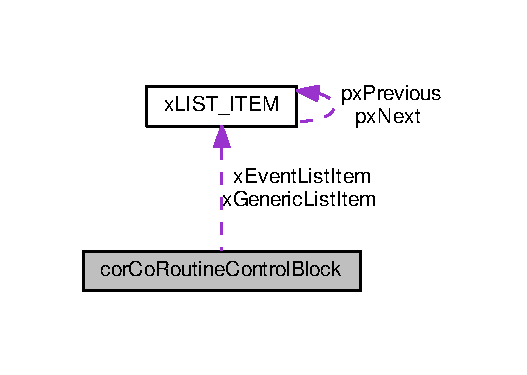
\includegraphics[width=253pt]{structcor_co_routine_control_block__coll__graph}
\end{center}
\end{figure}
\subsection*{Public Attributes}
\begin{DoxyCompactItemize}
\item 
\hyperlink{croutine_8h_a397a7505718dd366d8411ce324c49758}{cr\+C\+O\+R\+O\+U\+T\+I\+N\+E\+\_\+\+C\+O\+DE} \hyperlink{structcor_co_routine_control_block_acc98c7364cd88e8e034a5f9bba113832}{px\+Co\+Routine\+Function}
\item 
\hyperlink{list_8h_a1a62d469392f9bfe2443e7efab9c8398}{List\+Item\+\_\+t} \hyperlink{structcor_co_routine_control_block_aa2900494db8782eeb8ef12d482501406}{x\+Generic\+List\+Item}
\item 
\hyperlink{list_8h_a1a62d469392f9bfe2443e7efab9c8398}{List\+Item\+\_\+t} \hyperlink{structcor_co_routine_control_block_a105d316da0069f766acc3b210afed1b9}{x\+Event\+List\+Item}
\item 
\hyperlink{portmacro_8h_a646f89d4298e4f5afd522202b11cb2e6}{U\+Base\+Type\+\_\+t} \hyperlink{structcor_co_routine_control_block_a752101a5d41b5caa7fd5149436613c8f}{ux\+Priority}
\item 
\hyperlink{portmacro_8h_a646f89d4298e4f5afd522202b11cb2e6}{U\+Base\+Type\+\_\+t} \hyperlink{structcor_co_routine_control_block_a6c185cd2145f562fb570bea9b158fc81}{ux\+Index}
\item 
uint16\+\_\+t \hyperlink{structcor_co_routine_control_block_aa0d702ff5a23c61598fe13e5a78fb1dc}{ux\+State}
\end{DoxyCompactItemize}


\subsection{Detailed Description}


Definition at line 91 of file croutine.\+h.



\subsection{Member Data Documentation}
\index{cor\+Co\+Routine\+Control\+Block@{cor\+Co\+Routine\+Control\+Block}!px\+Co\+Routine\+Function@{px\+Co\+Routine\+Function}}
\index{px\+Co\+Routine\+Function@{px\+Co\+Routine\+Function}!cor\+Co\+Routine\+Control\+Block@{cor\+Co\+Routine\+Control\+Block}}
\subsubsection[{\texorpdfstring{px\+Co\+Routine\+Function}{pxCoRoutineFunction}}]{\setlength{\rightskip}{0pt plus 5cm}{\bf cr\+C\+O\+R\+O\+U\+T\+I\+N\+E\+\_\+\+C\+O\+DE} cor\+Co\+Routine\+Control\+Block\+::px\+Co\+Routine\+Function}\hypertarget{structcor_co_routine_control_block_acc98c7364cd88e8e034a5f9bba113832}{}\label{structcor_co_routine_control_block_acc98c7364cd88e8e034a5f9bba113832}


Definition at line 93 of file croutine.\+h.

\index{cor\+Co\+Routine\+Control\+Block@{cor\+Co\+Routine\+Control\+Block}!ux\+Index@{ux\+Index}}
\index{ux\+Index@{ux\+Index}!cor\+Co\+Routine\+Control\+Block@{cor\+Co\+Routine\+Control\+Block}}
\subsubsection[{\texorpdfstring{ux\+Index}{uxIndex}}]{\setlength{\rightskip}{0pt plus 5cm}{\bf U\+Base\+Type\+\_\+t} cor\+Co\+Routine\+Control\+Block\+::ux\+Index}\hypertarget{structcor_co_routine_control_block_a6c185cd2145f562fb570bea9b158fc81}{}\label{structcor_co_routine_control_block_a6c185cd2145f562fb570bea9b158fc81}


Definition at line 97 of file croutine.\+h.

\index{cor\+Co\+Routine\+Control\+Block@{cor\+Co\+Routine\+Control\+Block}!ux\+Priority@{ux\+Priority}}
\index{ux\+Priority@{ux\+Priority}!cor\+Co\+Routine\+Control\+Block@{cor\+Co\+Routine\+Control\+Block}}
\subsubsection[{\texorpdfstring{ux\+Priority}{uxPriority}}]{\setlength{\rightskip}{0pt plus 5cm}{\bf U\+Base\+Type\+\_\+t} cor\+Co\+Routine\+Control\+Block\+::ux\+Priority}\hypertarget{structcor_co_routine_control_block_a752101a5d41b5caa7fd5149436613c8f}{}\label{structcor_co_routine_control_block_a752101a5d41b5caa7fd5149436613c8f}


Definition at line 96 of file croutine.\+h.

\index{cor\+Co\+Routine\+Control\+Block@{cor\+Co\+Routine\+Control\+Block}!ux\+State@{ux\+State}}
\index{ux\+State@{ux\+State}!cor\+Co\+Routine\+Control\+Block@{cor\+Co\+Routine\+Control\+Block}}
\subsubsection[{\texorpdfstring{ux\+State}{uxState}}]{\setlength{\rightskip}{0pt plus 5cm}uint16\+\_\+t cor\+Co\+Routine\+Control\+Block\+::ux\+State}\hypertarget{structcor_co_routine_control_block_aa0d702ff5a23c61598fe13e5a78fb1dc}{}\label{structcor_co_routine_control_block_aa0d702ff5a23c61598fe13e5a78fb1dc}


Definition at line 98 of file croutine.\+h.

\index{cor\+Co\+Routine\+Control\+Block@{cor\+Co\+Routine\+Control\+Block}!x\+Event\+List\+Item@{x\+Event\+List\+Item}}
\index{x\+Event\+List\+Item@{x\+Event\+List\+Item}!cor\+Co\+Routine\+Control\+Block@{cor\+Co\+Routine\+Control\+Block}}
\subsubsection[{\texorpdfstring{x\+Event\+List\+Item}{xEventListItem}}]{\setlength{\rightskip}{0pt plus 5cm}{\bf List\+Item\+\_\+t} cor\+Co\+Routine\+Control\+Block\+::x\+Event\+List\+Item}\hypertarget{structcor_co_routine_control_block_a105d316da0069f766acc3b210afed1b9}{}\label{structcor_co_routine_control_block_a105d316da0069f766acc3b210afed1b9}


Definition at line 95 of file croutine.\+h.

\index{cor\+Co\+Routine\+Control\+Block@{cor\+Co\+Routine\+Control\+Block}!x\+Generic\+List\+Item@{x\+Generic\+List\+Item}}
\index{x\+Generic\+List\+Item@{x\+Generic\+List\+Item}!cor\+Co\+Routine\+Control\+Block@{cor\+Co\+Routine\+Control\+Block}}
\subsubsection[{\texorpdfstring{x\+Generic\+List\+Item}{xGenericListItem}}]{\setlength{\rightskip}{0pt plus 5cm}{\bf List\+Item\+\_\+t} cor\+Co\+Routine\+Control\+Block\+::x\+Generic\+List\+Item}\hypertarget{structcor_co_routine_control_block_aa2900494db8782eeb8ef12d482501406}{}\label{structcor_co_routine_control_block_aa2900494db8782eeb8ef12d482501406}


Definition at line 94 of file croutine.\+h.



The documentation for this struct was generated from the following file\+:\begin{DoxyCompactItemize}
\item 
/home/telemetria/git/workspaces/tinoc2\+\_\+firmware\+\_\+freertos/\+R\+T\+O\+S\+Demo/\+Source/\+Free\+R\+T\+O\+S\+\_\+\+Source/include/\hyperlink{croutine_8h}{croutine.\+h}\end{DoxyCompactItemize}

\hypertarget{struct_c_o_u_n_t___s_e_m___s_t_r_u_c_t}{}\section{C\+O\+U\+N\+T\+\_\+\+S\+E\+M\+\_\+\+S\+T\+R\+U\+CT Struct Reference}
\label{struct_c_o_u_n_t___s_e_m___s_t_r_u_c_t}\index{C\+O\+U\+N\+T\+\_\+\+S\+E\+M\+\_\+\+S\+T\+R\+U\+CT@{C\+O\+U\+N\+T\+\_\+\+S\+E\+M\+\_\+\+S\+T\+R\+U\+CT}}
\subsection*{Public Attributes}
\begin{DoxyCompactItemize}
\item 
\hyperlink{semphr_8h_ad88c6df4a04beedeac782918c8a332f5}{Semaphore\+Handle\+\_\+t} \hyperlink{struct_c_o_u_n_t___s_e_m___s_t_r_u_c_t_aafa3f894de13cc6a6c197790ca8d13e9}{x\+Semaphore}
\item 
\hyperlink{portmacro_8h_a646f89d4298e4f5afd522202b11cb2e6}{U\+Base\+Type\+\_\+t} \hyperlink{struct_c_o_u_n_t___s_e_m___s_t_r_u_c_t_a097f632892268e332a764d22416c7fca}{ux\+Expected\+Start\+Count}
\item 
\hyperlink{portmacro_8h_a646f89d4298e4f5afd522202b11cb2e6}{U\+Base\+Type\+\_\+t} \hyperlink{struct_c_o_u_n_t___s_e_m___s_t_r_u_c_t_a833a25b7177bc8bc7d04d2685459213e}{ux\+Loop\+Counter}
\end{DoxyCompactItemize}


\subsection{Detailed Description}


Definition at line 129 of file countsem.\+c.



\subsection{Member Data Documentation}
\index{C\+O\+U\+N\+T\+\_\+\+S\+E\+M\+\_\+\+S\+T\+R\+U\+CT@{C\+O\+U\+N\+T\+\_\+\+S\+E\+M\+\_\+\+S\+T\+R\+U\+CT}!ux\+Expected\+Start\+Count@{ux\+Expected\+Start\+Count}}
\index{ux\+Expected\+Start\+Count@{ux\+Expected\+Start\+Count}!C\+O\+U\+N\+T\+\_\+\+S\+E\+M\+\_\+\+S\+T\+R\+U\+CT@{C\+O\+U\+N\+T\+\_\+\+S\+E\+M\+\_\+\+S\+T\+R\+U\+CT}}
\subsubsection[{\texorpdfstring{ux\+Expected\+Start\+Count}{uxExpectedStartCount}}]{\setlength{\rightskip}{0pt plus 5cm}{\bf U\+Base\+Type\+\_\+t} C\+O\+U\+N\+T\+\_\+\+S\+E\+M\+\_\+\+S\+T\+R\+U\+C\+T\+::ux\+Expected\+Start\+Count}\hypertarget{struct_c_o_u_n_t___s_e_m___s_t_r_u_c_t_a097f632892268e332a764d22416c7fca}{}\label{struct_c_o_u_n_t___s_e_m___s_t_r_u_c_t_a097f632892268e332a764d22416c7fca}


Definition at line 137 of file countsem.\+c.

\index{C\+O\+U\+N\+T\+\_\+\+S\+E\+M\+\_\+\+S\+T\+R\+U\+CT@{C\+O\+U\+N\+T\+\_\+\+S\+E\+M\+\_\+\+S\+T\+R\+U\+CT}!ux\+Loop\+Counter@{ux\+Loop\+Counter}}
\index{ux\+Loop\+Counter@{ux\+Loop\+Counter}!C\+O\+U\+N\+T\+\_\+\+S\+E\+M\+\_\+\+S\+T\+R\+U\+CT@{C\+O\+U\+N\+T\+\_\+\+S\+E\+M\+\_\+\+S\+T\+R\+U\+CT}}
\subsubsection[{\texorpdfstring{ux\+Loop\+Counter}{uxLoopCounter}}]{\setlength{\rightskip}{0pt plus 5cm}{\bf U\+Base\+Type\+\_\+t} C\+O\+U\+N\+T\+\_\+\+S\+E\+M\+\_\+\+S\+T\+R\+U\+C\+T\+::ux\+Loop\+Counter}\hypertarget{struct_c_o_u_n_t___s_e_m___s_t_r_u_c_t_a833a25b7177bc8bc7d04d2685459213e}{}\label{struct_c_o_u_n_t___s_e_m___s_t_r_u_c_t_a833a25b7177bc8bc7d04d2685459213e}


Definition at line 141 of file countsem.\+c.

\index{C\+O\+U\+N\+T\+\_\+\+S\+E\+M\+\_\+\+S\+T\+R\+U\+CT@{C\+O\+U\+N\+T\+\_\+\+S\+E\+M\+\_\+\+S\+T\+R\+U\+CT}!x\+Semaphore@{x\+Semaphore}}
\index{x\+Semaphore@{x\+Semaphore}!C\+O\+U\+N\+T\+\_\+\+S\+E\+M\+\_\+\+S\+T\+R\+U\+CT@{C\+O\+U\+N\+T\+\_\+\+S\+E\+M\+\_\+\+S\+T\+R\+U\+CT}}
\subsubsection[{\texorpdfstring{x\+Semaphore}{xSemaphore}}]{\setlength{\rightskip}{0pt plus 5cm}{\bf Semaphore\+Handle\+\_\+t} C\+O\+U\+N\+T\+\_\+\+S\+E\+M\+\_\+\+S\+T\+R\+U\+C\+T\+::x\+Semaphore}\hypertarget{struct_c_o_u_n_t___s_e_m___s_t_r_u_c_t_aafa3f894de13cc6a6c197790ca8d13e9}{}\label{struct_c_o_u_n_t___s_e_m___s_t_r_u_c_t_aafa3f894de13cc6a6c197790ca8d13e9}


Definition at line 132 of file countsem.\+c.



The documentation for this struct was generated from the following file\+:\begin{DoxyCompactItemize}
\item 
/home/telemetria/git/workspaces/tinoc2\+\_\+firmware\+\_\+freertos/\+R\+T\+O\+S\+Demo/\+Source/\+Common\+\_\+\+Demo\+\_\+\+Tasks/\hyperlink{countsem_8c}{countsem.\+c}\end{DoxyCompactItemize}

\hypertarget{struct_heap_region}{}\section{Heap\+Region Struct Reference}
\label{struct_heap_region}\index{Heap\+Region@{Heap\+Region}}


{\ttfamily \#include $<$portable.\+h$>$}

\subsection*{Public Attributes}
\begin{DoxyCompactItemize}
\item 
uint8\+\_\+t $\ast$ \hyperlink{struct_heap_region_aab323508c34642ebfb884a68441d97fc}{puc\+Start\+Address}
\item 
size\+\_\+t \hyperlink{struct_heap_region_a5933b0fd422e70a92ceef839b89a757f}{x\+Size\+In\+Bytes}
\end{DoxyCompactItemize}


\subsection{Detailed Description}


Definition at line 148 of file portable.\+h.



\subsection{Member Data Documentation}
\index{Heap\+Region@{Heap\+Region}!puc\+Start\+Address@{puc\+Start\+Address}}
\index{puc\+Start\+Address@{puc\+Start\+Address}!Heap\+Region@{Heap\+Region}}
\subsubsection[{\texorpdfstring{puc\+Start\+Address}{pucStartAddress}}]{\setlength{\rightskip}{0pt plus 5cm}uint8\+\_\+t$\ast$ Heap\+Region\+::puc\+Start\+Address}\hypertarget{struct_heap_region_aab323508c34642ebfb884a68441d97fc}{}\label{struct_heap_region_aab323508c34642ebfb884a68441d97fc}


Definition at line 150 of file portable.\+h.

\index{Heap\+Region@{Heap\+Region}!x\+Size\+In\+Bytes@{x\+Size\+In\+Bytes}}
\index{x\+Size\+In\+Bytes@{x\+Size\+In\+Bytes}!Heap\+Region@{Heap\+Region}}
\subsubsection[{\texorpdfstring{x\+Size\+In\+Bytes}{xSizeInBytes}}]{\setlength{\rightskip}{0pt plus 5cm}size\+\_\+t Heap\+Region\+::x\+Size\+In\+Bytes}\hypertarget{struct_heap_region_a5933b0fd422e70a92ceef839b89a757f}{}\label{struct_heap_region_a5933b0fd422e70a92ceef839b89a757f}


Definition at line 151 of file portable.\+h.



The documentation for this struct was generated from the following file\+:\begin{DoxyCompactItemize}
\item 
/home/telemetria/git/workspaces/tinoc2\+\_\+firmware\+\_\+freertos/\+R\+T\+O\+S\+Demo/\+Source/\+Free\+R\+T\+O\+S\+\_\+\+Source/include/\hyperlink{portable_8h}{portable.\+h}\end{DoxyCompactItemize}

\hypertarget{struct_queue_definition}{}\section{Queue\+Definition Struct Reference}
\label{struct_queue_definition}\index{Queue\+Definition@{Queue\+Definition}}


Collaboration diagram for Queue\+Definition\+:\nopagebreak
\begin{figure}[H]
\begin{center}
\leavevmode
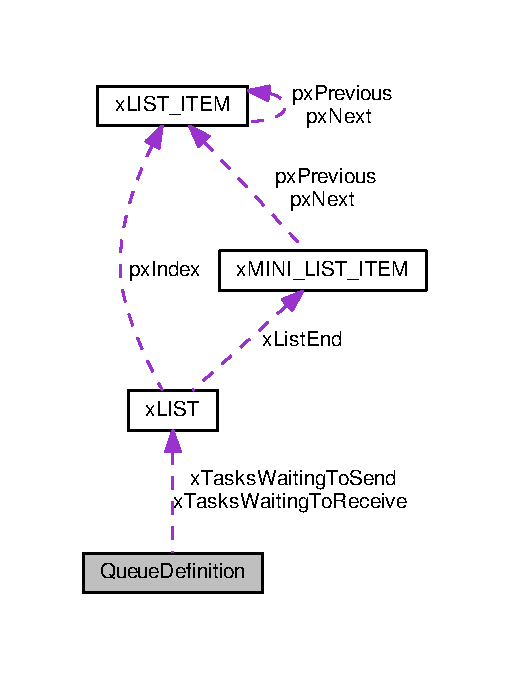
\includegraphics[width=245pt]{struct_queue_definition__coll__graph}
\end{center}
\end{figure}
\subsection*{Public Attributes}
\begin{DoxyCompactItemize}
\item 
int8\+\_\+t $\ast$ \hyperlink{struct_queue_definition_a487dc7e43b380c58212cba72bc33e0ed}{pc\+Head}
\item 
int8\+\_\+t $\ast$ \hyperlink{struct_queue_definition_a189dc1b16fc2152dd9441ea1a117b0ce}{pc\+Tail}
\item 
int8\+\_\+t $\ast$ \hyperlink{struct_queue_definition_abdf13cc013c8488848cee3fce4f0fed3}{pc\+Write\+To}
\item 
\begin{tabbing}
xx\=xx\=xx\=xx\=xx\=xx\=xx\=xx\=xx\=\kill
union \{\\
\>int8\_t $\ast$ \hyperlink{struct_queue_definition_a970cf73ab9c7382b581bc310b1d947d5}{pcReadFrom}\\
\>\hyperlink{portmacro_8h_a646f89d4298e4f5afd522202b11cb2e6}{UBaseType\_t} \hyperlink{struct_queue_definition_a2cf88e286477f6f89fe1009d722dc4cf}{uxRecursiveCallCount}\\
\} \hyperlink{struct_queue_definition_a3a2be4f333e88fd5bc1ddb7ae8441e28}{u}\\

\end{tabbing}\item 
\hyperlink{list_8h_afd590ef6400071b4d63d65ef90bea7f4}{List\+\_\+t} \hyperlink{struct_queue_definition_aaab135c4345cb0393d6ff3cd5164c7b2}{x\+Tasks\+Waiting\+To\+Send}
\item 
\hyperlink{list_8h_afd590ef6400071b4d63d65ef90bea7f4}{List\+\_\+t} \hyperlink{struct_queue_definition_af6d61526f77beee659cd604a0c473359}{x\+Tasks\+Waiting\+To\+Receive}
\item 
volatile \hyperlink{portmacro_8h_a646f89d4298e4f5afd522202b11cb2e6}{U\+Base\+Type\+\_\+t} \hyperlink{struct_queue_definition_a12b07a40152d0f21488ca06d362d13d1}{ux\+Messages\+Waiting}
\item 
\hyperlink{portmacro_8h_a646f89d4298e4f5afd522202b11cb2e6}{U\+Base\+Type\+\_\+t} \hyperlink{struct_queue_definition_ae80d17a812c669d4d41265b7f693988c}{ux\+Length}
\item 
\hyperlink{portmacro_8h_a646f89d4298e4f5afd522202b11cb2e6}{U\+Base\+Type\+\_\+t} \hyperlink{struct_queue_definition_a81bb7d3826909244baa9debf5a55abb0}{ux\+Item\+Size}
\item 
volatile int8\+\_\+t \hyperlink{struct_queue_definition_ac750a3f75a6e174adbc697e473a0dd13}{c\+Rx\+Lock}
\item 
volatile int8\+\_\+t \hyperlink{struct_queue_definition_a24ac3f0707f098da2a22244d843fcf82}{c\+Tx\+Lock}
\end{DoxyCompactItemize}


\subsection{Detailed Description}


Definition at line 130 of file queue.\+c.



\subsection{Member Data Documentation}
\index{Queue\+Definition@{Queue\+Definition}!c\+Rx\+Lock@{c\+Rx\+Lock}}
\index{c\+Rx\+Lock@{c\+Rx\+Lock}!Queue\+Definition@{Queue\+Definition}}
\subsubsection[{\texorpdfstring{c\+Rx\+Lock}{cRxLock}}]{\setlength{\rightskip}{0pt plus 5cm}volatile int8\+\_\+t Queue\+Definition\+::c\+Rx\+Lock}\hypertarget{struct_queue_definition_ac750a3f75a6e174adbc697e473a0dd13}{}\label{struct_queue_definition_ac750a3f75a6e174adbc697e473a0dd13}


Definition at line 149 of file queue.\+c.

\index{Queue\+Definition@{Queue\+Definition}!c\+Tx\+Lock@{c\+Tx\+Lock}}
\index{c\+Tx\+Lock@{c\+Tx\+Lock}!Queue\+Definition@{Queue\+Definition}}
\subsubsection[{\texorpdfstring{c\+Tx\+Lock}{cTxLock}}]{\setlength{\rightskip}{0pt plus 5cm}volatile int8\+\_\+t Queue\+Definition\+::c\+Tx\+Lock}\hypertarget{struct_queue_definition_a24ac3f0707f098da2a22244d843fcf82}{}\label{struct_queue_definition_a24ac3f0707f098da2a22244d843fcf82}


Definition at line 150 of file queue.\+c.

\index{Queue\+Definition@{Queue\+Definition}!pc\+Head@{pc\+Head}}
\index{pc\+Head@{pc\+Head}!Queue\+Definition@{Queue\+Definition}}
\subsubsection[{\texorpdfstring{pc\+Head}{pcHead}}]{\setlength{\rightskip}{0pt plus 5cm}int8\+\_\+t$\ast$ Queue\+Definition\+::pc\+Head}\hypertarget{struct_queue_definition_a487dc7e43b380c58212cba72bc33e0ed}{}\label{struct_queue_definition_a487dc7e43b380c58212cba72bc33e0ed}


Definition at line 132 of file queue.\+c.

\index{Queue\+Definition@{Queue\+Definition}!pc\+Read\+From@{pc\+Read\+From}}
\index{pc\+Read\+From@{pc\+Read\+From}!Queue\+Definition@{Queue\+Definition}}
\subsubsection[{\texorpdfstring{pc\+Read\+From}{pcReadFrom}}]{\setlength{\rightskip}{0pt plus 5cm}int8\+\_\+t$\ast$ Queue\+Definition\+::pc\+Read\+From}\hypertarget{struct_queue_definition_a970cf73ab9c7382b581bc310b1d947d5}{}\label{struct_queue_definition_a970cf73ab9c7382b581bc310b1d947d5}


Definition at line 138 of file queue.\+c.

\index{Queue\+Definition@{Queue\+Definition}!pc\+Tail@{pc\+Tail}}
\index{pc\+Tail@{pc\+Tail}!Queue\+Definition@{Queue\+Definition}}
\subsubsection[{\texorpdfstring{pc\+Tail}{pcTail}}]{\setlength{\rightskip}{0pt plus 5cm}int8\+\_\+t$\ast$ Queue\+Definition\+::pc\+Tail}\hypertarget{struct_queue_definition_a189dc1b16fc2152dd9441ea1a117b0ce}{}\label{struct_queue_definition_a189dc1b16fc2152dd9441ea1a117b0ce}


Definition at line 133 of file queue.\+c.

\index{Queue\+Definition@{Queue\+Definition}!pc\+Write\+To@{pc\+Write\+To}}
\index{pc\+Write\+To@{pc\+Write\+To}!Queue\+Definition@{Queue\+Definition}}
\subsubsection[{\texorpdfstring{pc\+Write\+To}{pcWriteTo}}]{\setlength{\rightskip}{0pt plus 5cm}int8\+\_\+t$\ast$ Queue\+Definition\+::pc\+Write\+To}\hypertarget{struct_queue_definition_abdf13cc013c8488848cee3fce4f0fed3}{}\label{struct_queue_definition_abdf13cc013c8488848cee3fce4f0fed3}


Definition at line 134 of file queue.\+c.

\index{Queue\+Definition@{Queue\+Definition}!u@{u}}
\index{u@{u}!Queue\+Definition@{Queue\+Definition}}
\subsubsection[{\texorpdfstring{u}{u}}]{\setlength{\rightskip}{0pt plus 5cm}union \{ ... \}   Queue\+Definition\+::u}\hypertarget{struct_queue_definition_a3a2be4f333e88fd5bc1ddb7ae8441e28}{}\label{struct_queue_definition_a3a2be4f333e88fd5bc1ddb7ae8441e28}
\index{Queue\+Definition@{Queue\+Definition}!ux\+Item\+Size@{ux\+Item\+Size}}
\index{ux\+Item\+Size@{ux\+Item\+Size}!Queue\+Definition@{Queue\+Definition}}
\subsubsection[{\texorpdfstring{ux\+Item\+Size}{uxItemSize}}]{\setlength{\rightskip}{0pt plus 5cm}{\bf U\+Base\+Type\+\_\+t} Queue\+Definition\+::ux\+Item\+Size}\hypertarget{struct_queue_definition_a81bb7d3826909244baa9debf5a55abb0}{}\label{struct_queue_definition_a81bb7d3826909244baa9debf5a55abb0}


Definition at line 147 of file queue.\+c.

\index{Queue\+Definition@{Queue\+Definition}!ux\+Length@{ux\+Length}}
\index{ux\+Length@{ux\+Length}!Queue\+Definition@{Queue\+Definition}}
\subsubsection[{\texorpdfstring{ux\+Length}{uxLength}}]{\setlength{\rightskip}{0pt plus 5cm}{\bf U\+Base\+Type\+\_\+t} Queue\+Definition\+::ux\+Length}\hypertarget{struct_queue_definition_ae80d17a812c669d4d41265b7f693988c}{}\label{struct_queue_definition_ae80d17a812c669d4d41265b7f693988c}


Definition at line 146 of file queue.\+c.

\index{Queue\+Definition@{Queue\+Definition}!ux\+Messages\+Waiting@{ux\+Messages\+Waiting}}
\index{ux\+Messages\+Waiting@{ux\+Messages\+Waiting}!Queue\+Definition@{Queue\+Definition}}
\subsubsection[{\texorpdfstring{ux\+Messages\+Waiting}{uxMessagesWaiting}}]{\setlength{\rightskip}{0pt plus 5cm}volatile {\bf U\+Base\+Type\+\_\+t} Queue\+Definition\+::ux\+Messages\+Waiting}\hypertarget{struct_queue_definition_a12b07a40152d0f21488ca06d362d13d1}{}\label{struct_queue_definition_a12b07a40152d0f21488ca06d362d13d1}


Definition at line 145 of file queue.\+c.

\index{Queue\+Definition@{Queue\+Definition}!ux\+Recursive\+Call\+Count@{ux\+Recursive\+Call\+Count}}
\index{ux\+Recursive\+Call\+Count@{ux\+Recursive\+Call\+Count}!Queue\+Definition@{Queue\+Definition}}
\subsubsection[{\texorpdfstring{ux\+Recursive\+Call\+Count}{uxRecursiveCallCount}}]{\setlength{\rightskip}{0pt plus 5cm}{\bf U\+Base\+Type\+\_\+t} Queue\+Definition\+::ux\+Recursive\+Call\+Count}\hypertarget{struct_queue_definition_a2cf88e286477f6f89fe1009d722dc4cf}{}\label{struct_queue_definition_a2cf88e286477f6f89fe1009d722dc4cf}


Definition at line 139 of file queue.\+c.

\index{Queue\+Definition@{Queue\+Definition}!x\+Tasks\+Waiting\+To\+Receive@{x\+Tasks\+Waiting\+To\+Receive}}
\index{x\+Tasks\+Waiting\+To\+Receive@{x\+Tasks\+Waiting\+To\+Receive}!Queue\+Definition@{Queue\+Definition}}
\subsubsection[{\texorpdfstring{x\+Tasks\+Waiting\+To\+Receive}{xTasksWaitingToReceive}}]{\setlength{\rightskip}{0pt plus 5cm}{\bf List\+\_\+t} Queue\+Definition\+::x\+Tasks\+Waiting\+To\+Receive}\hypertarget{struct_queue_definition_af6d61526f77beee659cd604a0c473359}{}\label{struct_queue_definition_af6d61526f77beee659cd604a0c473359}


Definition at line 143 of file queue.\+c.

\index{Queue\+Definition@{Queue\+Definition}!x\+Tasks\+Waiting\+To\+Send@{x\+Tasks\+Waiting\+To\+Send}}
\index{x\+Tasks\+Waiting\+To\+Send@{x\+Tasks\+Waiting\+To\+Send}!Queue\+Definition@{Queue\+Definition}}
\subsubsection[{\texorpdfstring{x\+Tasks\+Waiting\+To\+Send}{xTasksWaitingToSend}}]{\setlength{\rightskip}{0pt plus 5cm}{\bf List\+\_\+t} Queue\+Definition\+::x\+Tasks\+Waiting\+To\+Send}\hypertarget{struct_queue_definition_aaab135c4345cb0393d6ff3cd5164c7b2}{}\label{struct_queue_definition_aaab135c4345cb0393d6ff3cd5164c7b2}


Definition at line 142 of file queue.\+c.



The documentation for this struct was generated from the following file\+:\begin{DoxyCompactItemize}
\item 
/home/telemetria/git/workspaces/tinoc2\+\_\+firmware\+\_\+freertos/\+R\+T\+O\+S\+Demo/\+Source/\+Free\+R\+T\+O\+S\+\_\+\+Source/\hyperlink{queue_8c}{queue.\+c}\end{DoxyCompactItemize}

\hypertarget{structt__cola}{}\section{t\+\_\+cola Struct Reference}
\label{structt__cola}\index{t\+\_\+cola@{t\+\_\+cola}}


{\ttfamily \#include $<$colas.\+h$>$}

\subsection*{Public Attributes}
\begin{DoxyCompactItemize}
\item 
uint8\+\_\+t \hyperlink{structt__cola_a036c41abaec1f17327ac2c8c797e131b}{buffer} \mbox{[}\hyperlink{colas_8h_ac71c7234de240e3781fe2467040fb3b0}{B\+U\+F\+F\+E\+R\+\_\+N}\mbox{]}
\begin{DoxyCompactList}\small\item\em Buffer de la cola. \end{DoxyCompactList}\item 
uint8\+\_\+t \hyperlink{structt__cola_ad3a0ddb896e8181a52ca74637016f1c7}{ini}
\item 
uint8\+\_\+t \hyperlink{structt__cola_a7a826546e1b03d5efc5ce211cc867008}{fin}
\item 
\hyperlink{colas_8h_adcf7b87b5431386461b2c790e786729a}{t\+\_\+estado\+\_\+buffer} \hyperlink{structt__cola_ad0292a1aa7a79b98d63083ed0d732df6}{estado\+\_\+buffer}
\item 
uint8\+\_\+t \hyperlink{structt__cola_ab28a0c32685544a21076d390d2d9f800}{datos\+\_\+nuevos}
\end{DoxyCompactItemize}


\subsection{Detailed Description}


Definition at line 47 of file colas.\+h.



\subsection{Member Data Documentation}
\index{t\+\_\+cola@{t\+\_\+cola}!buffer@{buffer}}
\index{buffer@{buffer}!t\+\_\+cola@{t\+\_\+cola}}
\subsubsection[{\texorpdfstring{buffer}{buffer}}]{\setlength{\rightskip}{0pt plus 5cm}uint8\+\_\+t t\+\_\+cola\+::buffer\mbox{[}{\bf B\+U\+F\+F\+E\+R\+\_\+N}\mbox{]}}\hypertarget{structt__cola_a036c41abaec1f17327ac2c8c797e131b}{}\label{structt__cola_a036c41abaec1f17327ac2c8c797e131b}


Buffer de la cola. 



Definition at line 50 of file colas.\+h.

\index{t\+\_\+cola@{t\+\_\+cola}!datos\+\_\+nuevos@{datos\+\_\+nuevos}}
\index{datos\+\_\+nuevos@{datos\+\_\+nuevos}!t\+\_\+cola@{t\+\_\+cola}}
\subsubsection[{\texorpdfstring{datos\+\_\+nuevos}{datos_nuevos}}]{\setlength{\rightskip}{0pt plus 5cm}uint8\+\_\+t t\+\_\+cola\+::datos\+\_\+nuevos}\hypertarget{structt__cola_ab28a0c32685544a21076d390d2d9f800}{}\label{structt__cola_ab28a0c32685544a21076d390d2d9f800}


Definition at line 53 of file colas.\+h.

\index{t\+\_\+cola@{t\+\_\+cola}!estado\+\_\+buffer@{estado\+\_\+buffer}}
\index{estado\+\_\+buffer@{estado\+\_\+buffer}!t\+\_\+cola@{t\+\_\+cola}}
\subsubsection[{\texorpdfstring{estado\+\_\+buffer}{estado_buffer}}]{\setlength{\rightskip}{0pt plus 5cm}{\bf t\+\_\+estado\+\_\+buffer} t\+\_\+cola\+::estado\+\_\+buffer}\hypertarget{structt__cola_ad0292a1aa7a79b98d63083ed0d732df6}{}\label{structt__cola_ad0292a1aa7a79b98d63083ed0d732df6}


Definition at line 52 of file colas.\+h.

\index{t\+\_\+cola@{t\+\_\+cola}!fin@{fin}}
\index{fin@{fin}!t\+\_\+cola@{t\+\_\+cola}}
\subsubsection[{\texorpdfstring{fin}{fin}}]{\setlength{\rightskip}{0pt plus 5cm}uint8\+\_\+t t\+\_\+cola\+::fin}\hypertarget{structt__cola_a7a826546e1b03d5efc5ce211cc867008}{}\label{structt__cola_a7a826546e1b03d5efc5ce211cc867008}


Definition at line 51 of file colas.\+h.

\index{t\+\_\+cola@{t\+\_\+cola}!ini@{ini}}
\index{ini@{ini}!t\+\_\+cola@{t\+\_\+cola}}
\subsubsection[{\texorpdfstring{ini}{ini}}]{\setlength{\rightskip}{0pt plus 5cm}uint8\+\_\+t t\+\_\+cola\+::ini}\hypertarget{structt__cola_ad3a0ddb896e8181a52ca74637016f1c7}{}\label{structt__cola_ad3a0ddb896e8181a52ca74637016f1c7}


Definition at line 51 of file colas.\+h.



The documentation for this struct was generated from the following file\+:\begin{DoxyCompactItemize}
\item 
/home/telemetria/git/workspaces/tinoc2\+\_\+firmware\+\_\+freertos/\+R\+T\+O\+S\+Demo/\+Source/\+U\+A\+R\+T/\hyperlink{colas_8h}{colas.\+h}\end{DoxyCompactItemize}

\hypertarget{structtsk_task_control_block}{}\section{tsk\+Task\+Control\+Block Struct Reference}
\label{structtsk_task_control_block}\index{tsk\+Task\+Control\+Block@{tsk\+Task\+Control\+Block}}


Collaboration diagram for tsk\+Task\+Control\+Block\+:\nopagebreak
\begin{figure}[H]
\begin{center}
\leavevmode
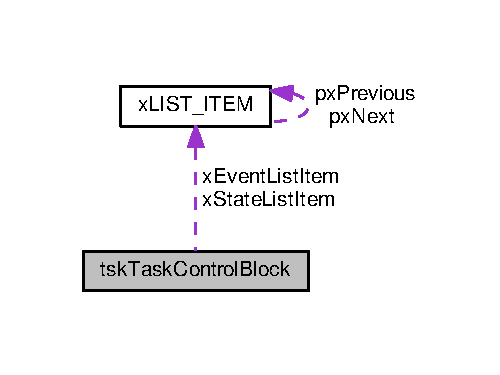
\includegraphics[width=240pt]{structtsk_task_control_block__coll__graph}
\end{center}
\end{figure}
\subsection*{Public Attributes}
\begin{DoxyCompactItemize}
\item 
volatile \hyperlink{portmacro_8h_a84e9a8ba132feed0b2401c1f4e2ac63c}{Stack\+Type\+\_\+t} $\ast$ \hyperlink{structtsk_task_control_block_a429a186c7f8e34aba1eef5e12d215b90}{px\+Top\+Of\+Stack}
\item 
\hyperlink{list_8h_a1a62d469392f9bfe2443e7efab9c8398}{List\+Item\+\_\+t} \hyperlink{structtsk_task_control_block_a16e0d20425d53ac78537e1fdb8834cf6}{x\+State\+List\+Item}
\item 
\hyperlink{list_8h_a1a62d469392f9bfe2443e7efab9c8398}{List\+Item\+\_\+t} \hyperlink{structtsk_task_control_block_a1a1612b6081a13683808284d93a9b28f}{x\+Event\+List\+Item}
\item 
\hyperlink{portmacro_8h_a646f89d4298e4f5afd522202b11cb2e6}{U\+Base\+Type\+\_\+t} \hyperlink{structtsk_task_control_block_a79187811e3d2a15595942e3b44237d85}{ux\+Priority}
\item 
\hyperlink{portmacro_8h_a84e9a8ba132feed0b2401c1f4e2ac63c}{Stack\+Type\+\_\+t} $\ast$ \hyperlink{structtsk_task_control_block_a9a0d71a9f95dd0609f9911d9efd79134}{px\+Stack}
\item 
char \hyperlink{structtsk_task_control_block_a67d61291794f38afb5be5132078bc24f}{pc\+Task\+Name} \mbox{[}\hyperlink{_free_r_t_o_s_config_8h_ac388dc4041aab6997348828eb27fc1a8}{config\+M\+A\+X\+\_\+\+T\+A\+S\+K\+\_\+\+N\+A\+M\+E\+\_\+\+L\+EN}\mbox{]}
\end{DoxyCompactItemize}


\subsection{Detailed Description}


Definition at line 293 of file tasks.\+c.



\subsection{Member Data Documentation}
\index{tsk\+Task\+Control\+Block@{tsk\+Task\+Control\+Block}!pc\+Task\+Name@{pc\+Task\+Name}}
\index{pc\+Task\+Name@{pc\+Task\+Name}!tsk\+Task\+Control\+Block@{tsk\+Task\+Control\+Block}}
\subsubsection[{\texorpdfstring{pc\+Task\+Name}{pcTaskName}}]{\setlength{\rightskip}{0pt plus 5cm}char tsk\+Task\+Control\+Block\+::pc\+Task\+Name\mbox{[}{\bf config\+M\+A\+X\+\_\+\+T\+A\+S\+K\+\_\+\+N\+A\+M\+E\+\_\+\+L\+EN}\mbox{]}}\hypertarget{structtsk_task_control_block_a67d61291794f38afb5be5132078bc24f}{}\label{structtsk_task_control_block_a67d61291794f38afb5be5132078bc24f}


Definition at line 305 of file tasks.\+c.

\index{tsk\+Task\+Control\+Block@{tsk\+Task\+Control\+Block}!px\+Stack@{px\+Stack}}
\index{px\+Stack@{px\+Stack}!tsk\+Task\+Control\+Block@{tsk\+Task\+Control\+Block}}
\subsubsection[{\texorpdfstring{px\+Stack}{pxStack}}]{\setlength{\rightskip}{0pt plus 5cm}{\bf Stack\+Type\+\_\+t}$\ast$ tsk\+Task\+Control\+Block\+::px\+Stack}\hypertarget{structtsk_task_control_block_a9a0d71a9f95dd0609f9911d9efd79134}{}\label{structtsk_task_control_block_a9a0d71a9f95dd0609f9911d9efd79134}


Definition at line 304 of file tasks.\+c.

\index{tsk\+Task\+Control\+Block@{tsk\+Task\+Control\+Block}!px\+Top\+Of\+Stack@{px\+Top\+Of\+Stack}}
\index{px\+Top\+Of\+Stack@{px\+Top\+Of\+Stack}!tsk\+Task\+Control\+Block@{tsk\+Task\+Control\+Block}}
\subsubsection[{\texorpdfstring{px\+Top\+Of\+Stack}{pxTopOfStack}}]{\setlength{\rightskip}{0pt plus 5cm}volatile {\bf Stack\+Type\+\_\+t}$\ast$ tsk\+Task\+Control\+Block\+::px\+Top\+Of\+Stack}\hypertarget{structtsk_task_control_block_a429a186c7f8e34aba1eef5e12d215b90}{}\label{structtsk_task_control_block_a429a186c7f8e34aba1eef5e12d215b90}


Definition at line 295 of file tasks.\+c.

\index{tsk\+Task\+Control\+Block@{tsk\+Task\+Control\+Block}!ux\+Priority@{ux\+Priority}}
\index{ux\+Priority@{ux\+Priority}!tsk\+Task\+Control\+Block@{tsk\+Task\+Control\+Block}}
\subsubsection[{\texorpdfstring{ux\+Priority}{uxPriority}}]{\setlength{\rightskip}{0pt plus 5cm}{\bf U\+Base\+Type\+\_\+t} tsk\+Task\+Control\+Block\+::ux\+Priority}\hypertarget{structtsk_task_control_block_a79187811e3d2a15595942e3b44237d85}{}\label{structtsk_task_control_block_a79187811e3d2a15595942e3b44237d85}


Definition at line 303 of file tasks.\+c.

\index{tsk\+Task\+Control\+Block@{tsk\+Task\+Control\+Block}!x\+Event\+List\+Item@{x\+Event\+List\+Item}}
\index{x\+Event\+List\+Item@{x\+Event\+List\+Item}!tsk\+Task\+Control\+Block@{tsk\+Task\+Control\+Block}}
\subsubsection[{\texorpdfstring{x\+Event\+List\+Item}{xEventListItem}}]{\setlength{\rightskip}{0pt plus 5cm}{\bf List\+Item\+\_\+t} tsk\+Task\+Control\+Block\+::x\+Event\+List\+Item}\hypertarget{structtsk_task_control_block_a1a1612b6081a13683808284d93a9b28f}{}\label{structtsk_task_control_block_a1a1612b6081a13683808284d93a9b28f}


Definition at line 302 of file tasks.\+c.

\index{tsk\+Task\+Control\+Block@{tsk\+Task\+Control\+Block}!x\+State\+List\+Item@{x\+State\+List\+Item}}
\index{x\+State\+List\+Item@{x\+State\+List\+Item}!tsk\+Task\+Control\+Block@{tsk\+Task\+Control\+Block}}
\subsubsection[{\texorpdfstring{x\+State\+List\+Item}{xStateListItem}}]{\setlength{\rightskip}{0pt plus 5cm}{\bf List\+Item\+\_\+t} tsk\+Task\+Control\+Block\+::x\+State\+List\+Item}\hypertarget{structtsk_task_control_block_a16e0d20425d53ac78537e1fdb8834cf6}{}\label{structtsk_task_control_block_a16e0d20425d53ac78537e1fdb8834cf6}


Definition at line 301 of file tasks.\+c.



The documentation for this struct was generated from the following file\+:\begin{DoxyCompactItemize}
\item 
/home/telemetria/git/workspaces/tinoc2\+\_\+firmware\+\_\+freertos/\+R\+T\+O\+S\+Demo/\+Source/\+Free\+R\+T\+O\+S\+\_\+\+Source/\hyperlink{tasks_8c}{tasks.\+c}\end{DoxyCompactItemize}

\hypertarget{structx_l_i_s_t}{}\section{x\+L\+I\+ST Struct Reference}
\label{structx_l_i_s_t}\index{x\+L\+I\+ST@{x\+L\+I\+ST}}


{\ttfamily \#include $<$list.\+h$>$}



Collaboration diagram for x\+L\+I\+ST\+:\nopagebreak
\begin{figure}[H]
\begin{center}
\leavevmode
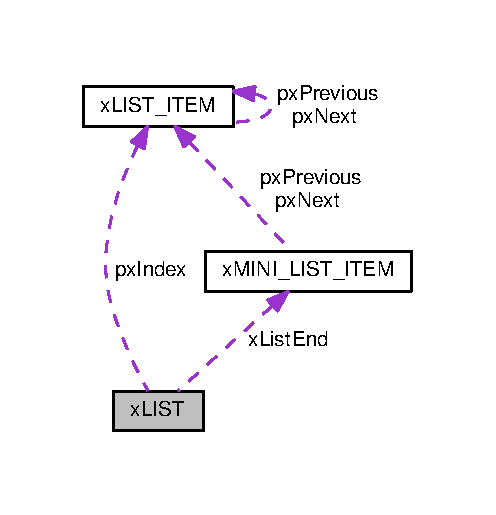
\includegraphics[width=238pt]{structx_l_i_s_t__coll__graph}
\end{center}
\end{figure}
\subsection*{Public Attributes}
\begin{DoxyCompactItemize}
\item 
\hyperlink{list_8h_a3a52b5a4f70d3a07e37a5814a23ba880}{list\+F\+I\+R\+S\+T\+\_\+\+L\+I\+S\+T\+\_\+\+I\+N\+T\+E\+G\+R\+I\+T\+Y\+\_\+\+C\+H\+E\+C\+K\+\_\+\+V\+A\+L\+UE} \hyperlink{list_8h_a2d5de557c5561c8980d1bf51d87d8cba}{config\+L\+I\+S\+T\+\_\+\+V\+O\+L\+A\+T\+I\+LE} \hyperlink{portmacro_8h_a646f89d4298e4f5afd522202b11cb2e6}{U\+Base\+Type\+\_\+t} \hyperlink{structx_l_i_s_t_aa5cb7cdc699e1252af0441e46e427a03}{ux\+Number\+Of\+Items}
\item 
\hyperlink{list_8h_a1a62d469392f9bfe2443e7efab9c8398}{List\+Item\+\_\+t} $\ast$\hyperlink{list_8h_a2d5de557c5561c8980d1bf51d87d8cba}{config\+L\+I\+S\+T\+\_\+\+V\+O\+L\+A\+T\+I\+LE} \hyperlink{structx_l_i_s_t_a7bf64d87701493b4c8c5c977682500d7}{px\+Index}
\item 
\hyperlink{list_8h_a542a8d55e98bc407593979e61f83cd02}{Mini\+List\+Item\+\_\+t} \hyperlink{structx_l_i_s_t_a49ad62fa153126e27e273811167b336a}{x\+List\+End}
\end{DoxyCompactItemize}


\subsection{Detailed Description}


Definition at line 205 of file list.\+h.



\subsection{Member Data Documentation}
\index{x\+L\+I\+ST@{x\+L\+I\+ST}!px\+Index@{px\+Index}}
\index{px\+Index@{px\+Index}!x\+L\+I\+ST@{x\+L\+I\+ST}}
\subsubsection[{\texorpdfstring{px\+Index}{pxIndex}}]{\setlength{\rightskip}{0pt plus 5cm}{\bf List\+Item\+\_\+t}$\ast$ {\bf config\+L\+I\+S\+T\+\_\+\+V\+O\+L\+A\+T\+I\+LE} x\+L\+I\+S\+T\+::px\+Index}\hypertarget{structx_l_i_s_t_a7bf64d87701493b4c8c5c977682500d7}{}\label{structx_l_i_s_t_a7bf64d87701493b4c8c5c977682500d7}


Definition at line 209 of file list.\+h.

\index{x\+L\+I\+ST@{x\+L\+I\+ST}!ux\+Number\+Of\+Items@{ux\+Number\+Of\+Items}}
\index{ux\+Number\+Of\+Items@{ux\+Number\+Of\+Items}!x\+L\+I\+ST@{x\+L\+I\+ST}}
\subsubsection[{\texorpdfstring{ux\+Number\+Of\+Items}{uxNumberOfItems}}]{\setlength{\rightskip}{0pt plus 5cm}{\bf list\+F\+I\+R\+S\+T\+\_\+\+L\+I\+S\+T\+\_\+\+I\+N\+T\+E\+G\+R\+I\+T\+Y\+\_\+\+C\+H\+E\+C\+K\+\_\+\+V\+A\+L\+UE} {\bf config\+L\+I\+S\+T\+\_\+\+V\+O\+L\+A\+T\+I\+LE} {\bf U\+Base\+Type\+\_\+t} x\+L\+I\+S\+T\+::ux\+Number\+Of\+Items}\hypertarget{structx_l_i_s_t_aa5cb7cdc699e1252af0441e46e427a03}{}\label{structx_l_i_s_t_aa5cb7cdc699e1252af0441e46e427a03}


Definition at line 208 of file list.\+h.

\index{x\+L\+I\+ST@{x\+L\+I\+ST}!x\+List\+End@{x\+List\+End}}
\index{x\+List\+End@{x\+List\+End}!x\+L\+I\+ST@{x\+L\+I\+ST}}
\subsubsection[{\texorpdfstring{x\+List\+End}{xListEnd}}]{\setlength{\rightskip}{0pt plus 5cm}{\bf Mini\+List\+Item\+\_\+t} x\+L\+I\+S\+T\+::x\+List\+End}\hypertarget{structx_l_i_s_t_a49ad62fa153126e27e273811167b336a}{}\label{structx_l_i_s_t_a49ad62fa153126e27e273811167b336a}


Definition at line 210 of file list.\+h.



The documentation for this struct was generated from the following file\+:\begin{DoxyCompactItemize}
\item 
/home/telemetria/git/workspaces/tinoc2\+\_\+firmware\+\_\+freertos/\+R\+T\+O\+S\+Demo/\+Source/\+Free\+R\+T\+O\+S\+\_\+\+Source/include/\hyperlink{list_8h}{list.\+h}\end{DoxyCompactItemize}

\hypertarget{structx_l_i_s_t___i_t_e_m}{}\section{x\+L\+I\+S\+T\+\_\+\+I\+T\+EM Struct Reference}
\label{structx_l_i_s_t___i_t_e_m}\index{x\+L\+I\+S\+T\+\_\+\+I\+T\+EM@{x\+L\+I\+S\+T\+\_\+\+I\+T\+EM}}


{\ttfamily \#include $<$list.\+h$>$}



Collaboration diagram for x\+L\+I\+S\+T\+\_\+\+I\+T\+EM\+:\nopagebreak
\begin{figure}[H]
\begin{center}
\leavevmode
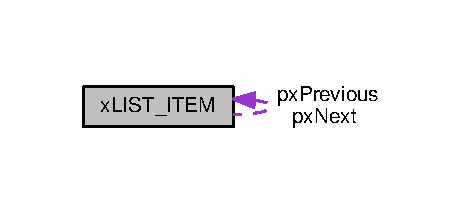
\includegraphics[width=222pt]{structx_l_i_s_t___i_t_e_m__coll__graph}
\end{center}
\end{figure}
\subsection*{Public Attributes}
\begin{DoxyCompactItemize}
\item 
\hyperlink{list_8h_a3611bd5d5d87cb26ac1dc7a4852b94a0}{list\+F\+I\+R\+S\+T\+\_\+\+L\+I\+S\+T\+\_\+\+I\+T\+E\+M\+\_\+\+I\+N\+T\+E\+G\+R\+I\+T\+Y\+\_\+\+C\+H\+E\+C\+K\+\_\+\+V\+A\+L\+UE} \hyperlink{list_8h_a2d5de557c5561c8980d1bf51d87d8cba}{config\+L\+I\+S\+T\+\_\+\+V\+O\+L\+A\+T\+I\+LE} \hyperlink{portmacro_8h_aa69c48c6e902ce54f70886e6573c92a9}{Tick\+Type\+\_\+t} \hyperlink{structx_l_i_s_t___i_t_e_m_a9b1f26de79f9da1403ca3ebc7a2e653a}{x\+Item\+Value}
\item 
struct \hyperlink{structx_l_i_s_t___i_t_e_m}{x\+L\+I\+S\+T\+\_\+\+I\+T\+EM} $\ast$\hyperlink{list_8h_a2d5de557c5561c8980d1bf51d87d8cba}{config\+L\+I\+S\+T\+\_\+\+V\+O\+L\+A\+T\+I\+LE} \hyperlink{structx_l_i_s_t___i_t_e_m_a03713c4ee953ef5ca6adbec883720c60}{px\+Next}
\item 
struct \hyperlink{structx_l_i_s_t___i_t_e_m}{x\+L\+I\+S\+T\+\_\+\+I\+T\+EM} $\ast$\hyperlink{list_8h_a2d5de557c5561c8980d1bf51d87d8cba}{config\+L\+I\+S\+T\+\_\+\+V\+O\+L\+A\+T\+I\+LE} \hyperlink{structx_l_i_s_t___i_t_e_m_ae8e553eae41010a8e41c66d76c94110b}{px\+Previous}
\item 
void $\ast$ \hyperlink{structx_l_i_s_t___i_t_e_m_aeb3110b50fe0dbce826d929b27b5ddb1}{pv\+Owner}
\item 
void $\ast$\hyperlink{list_8h_a2d5de557c5561c8980d1bf51d87d8cba}{config\+L\+I\+S\+T\+\_\+\+V\+O\+L\+A\+T\+I\+LE} \hyperlink{structx_l_i_s_t___i_t_e_m_a341462d06236aa07eaf1a864e4b59951}{pv\+Container}
\end{DoxyCompactItemize}


\subsection{Detailed Description}


Definition at line 181 of file list.\+h.



\subsection{Member Data Documentation}
\index{x\+L\+I\+S\+T\+\_\+\+I\+T\+EM@{x\+L\+I\+S\+T\+\_\+\+I\+T\+EM}!pv\+Container@{pv\+Container}}
\index{pv\+Container@{pv\+Container}!x\+L\+I\+S\+T\+\_\+\+I\+T\+EM@{x\+L\+I\+S\+T\+\_\+\+I\+T\+EM}}
\subsubsection[{\texorpdfstring{pv\+Container}{pvContainer}}]{\setlength{\rightskip}{0pt plus 5cm}void$\ast$ {\bf config\+L\+I\+S\+T\+\_\+\+V\+O\+L\+A\+T\+I\+LE} x\+L\+I\+S\+T\+\_\+\+I\+T\+E\+M\+::pv\+Container}\hypertarget{structx_l_i_s_t___i_t_e_m_a341462d06236aa07eaf1a864e4b59951}{}\label{structx_l_i_s_t___i_t_e_m_a341462d06236aa07eaf1a864e4b59951}


Definition at line 188 of file list.\+h.

\index{x\+L\+I\+S\+T\+\_\+\+I\+T\+EM@{x\+L\+I\+S\+T\+\_\+\+I\+T\+EM}!pv\+Owner@{pv\+Owner}}
\index{pv\+Owner@{pv\+Owner}!x\+L\+I\+S\+T\+\_\+\+I\+T\+EM@{x\+L\+I\+S\+T\+\_\+\+I\+T\+EM}}
\subsubsection[{\texorpdfstring{pv\+Owner}{pvOwner}}]{\setlength{\rightskip}{0pt plus 5cm}void$\ast$ x\+L\+I\+S\+T\+\_\+\+I\+T\+E\+M\+::pv\+Owner}\hypertarget{structx_l_i_s_t___i_t_e_m_aeb3110b50fe0dbce826d929b27b5ddb1}{}\label{structx_l_i_s_t___i_t_e_m_aeb3110b50fe0dbce826d929b27b5ddb1}


Definition at line 187 of file list.\+h.

\index{x\+L\+I\+S\+T\+\_\+\+I\+T\+EM@{x\+L\+I\+S\+T\+\_\+\+I\+T\+EM}!px\+Next@{px\+Next}}
\index{px\+Next@{px\+Next}!x\+L\+I\+S\+T\+\_\+\+I\+T\+EM@{x\+L\+I\+S\+T\+\_\+\+I\+T\+EM}}
\subsubsection[{\texorpdfstring{px\+Next}{pxNext}}]{\setlength{\rightskip}{0pt plus 5cm}struct {\bf x\+L\+I\+S\+T\+\_\+\+I\+T\+EM}$\ast$ {\bf config\+L\+I\+S\+T\+\_\+\+V\+O\+L\+A\+T\+I\+LE} x\+L\+I\+S\+T\+\_\+\+I\+T\+E\+M\+::px\+Next}\hypertarget{structx_l_i_s_t___i_t_e_m_a03713c4ee953ef5ca6adbec883720c60}{}\label{structx_l_i_s_t___i_t_e_m_a03713c4ee953ef5ca6adbec883720c60}


Definition at line 185 of file list.\+h.

\index{x\+L\+I\+S\+T\+\_\+\+I\+T\+EM@{x\+L\+I\+S\+T\+\_\+\+I\+T\+EM}!px\+Previous@{px\+Previous}}
\index{px\+Previous@{px\+Previous}!x\+L\+I\+S\+T\+\_\+\+I\+T\+EM@{x\+L\+I\+S\+T\+\_\+\+I\+T\+EM}}
\subsubsection[{\texorpdfstring{px\+Previous}{pxPrevious}}]{\setlength{\rightskip}{0pt plus 5cm}struct {\bf x\+L\+I\+S\+T\+\_\+\+I\+T\+EM}$\ast$ {\bf config\+L\+I\+S\+T\+\_\+\+V\+O\+L\+A\+T\+I\+LE} x\+L\+I\+S\+T\+\_\+\+I\+T\+E\+M\+::px\+Previous}\hypertarget{structx_l_i_s_t___i_t_e_m_ae8e553eae41010a8e41c66d76c94110b}{}\label{structx_l_i_s_t___i_t_e_m_ae8e553eae41010a8e41c66d76c94110b}


Definition at line 186 of file list.\+h.

\index{x\+L\+I\+S\+T\+\_\+\+I\+T\+EM@{x\+L\+I\+S\+T\+\_\+\+I\+T\+EM}!x\+Item\+Value@{x\+Item\+Value}}
\index{x\+Item\+Value@{x\+Item\+Value}!x\+L\+I\+S\+T\+\_\+\+I\+T\+EM@{x\+L\+I\+S\+T\+\_\+\+I\+T\+EM}}
\subsubsection[{\texorpdfstring{x\+Item\+Value}{xItemValue}}]{\setlength{\rightskip}{0pt plus 5cm}{\bf list\+F\+I\+R\+S\+T\+\_\+\+L\+I\+S\+T\+\_\+\+I\+T\+E\+M\+\_\+\+I\+N\+T\+E\+G\+R\+I\+T\+Y\+\_\+\+C\+H\+E\+C\+K\+\_\+\+V\+A\+L\+UE} {\bf config\+L\+I\+S\+T\+\_\+\+V\+O\+L\+A\+T\+I\+LE} {\bf Tick\+Type\+\_\+t} x\+L\+I\+S\+T\+\_\+\+I\+T\+E\+M\+::x\+Item\+Value}\hypertarget{structx_l_i_s_t___i_t_e_m_a9b1f26de79f9da1403ca3ebc7a2e653a}{}\label{structx_l_i_s_t___i_t_e_m_a9b1f26de79f9da1403ca3ebc7a2e653a}


Definition at line 184 of file list.\+h.



The documentation for this struct was generated from the following file\+:\begin{DoxyCompactItemize}
\item 
/home/telemetria/git/workspaces/tinoc2\+\_\+firmware\+\_\+freertos/\+R\+T\+O\+S\+Demo/\+Source/\+Free\+R\+T\+O\+S\+\_\+\+Source/include/\hyperlink{list_8h}{list.\+h}\end{DoxyCompactItemize}

\hypertarget{structx_m_e_m_o_r_y___r_e_g_i_o_n}{}\section{x\+M\+E\+M\+O\+R\+Y\+\_\+\+R\+E\+G\+I\+ON Struct Reference}
\label{structx_m_e_m_o_r_y___r_e_g_i_o_n}\index{x\+M\+E\+M\+O\+R\+Y\+\_\+\+R\+E\+G\+I\+ON@{x\+M\+E\+M\+O\+R\+Y\+\_\+\+R\+E\+G\+I\+ON}}


{\ttfamily \#include $<$task.\+h$>$}

\subsection*{Public Attributes}
\begin{DoxyCompactItemize}
\item 
void $\ast$ \hyperlink{structx_m_e_m_o_r_y___r_e_g_i_o_n_a228036bbfdbc38f170e45deadb166172}{pv\+Base\+Address}
\item 
uint32\+\_\+t \hyperlink{structx_m_e_m_o_r_y___r_e_g_i_o_n_a97e59578d3c4c46270d33e7206258a65}{ul\+Length\+In\+Bytes}
\item 
uint32\+\_\+t \hyperlink{structx_m_e_m_o_r_y___r_e_g_i_o_n_a6ba180553e9a318f23acc5f4664934e3}{ul\+Parameters}
\end{DoxyCompactItemize}


\subsection{Detailed Description}


Definition at line 144 of file task.\+h.



\subsection{Member Data Documentation}
\index{x\+M\+E\+M\+O\+R\+Y\+\_\+\+R\+E\+G\+I\+ON@{x\+M\+E\+M\+O\+R\+Y\+\_\+\+R\+E\+G\+I\+ON}!pv\+Base\+Address@{pv\+Base\+Address}}
\index{pv\+Base\+Address@{pv\+Base\+Address}!x\+M\+E\+M\+O\+R\+Y\+\_\+\+R\+E\+G\+I\+ON@{x\+M\+E\+M\+O\+R\+Y\+\_\+\+R\+E\+G\+I\+ON}}
\subsubsection[{\texorpdfstring{pv\+Base\+Address}{pvBaseAddress}}]{\setlength{\rightskip}{0pt plus 5cm}void$\ast$ x\+M\+E\+M\+O\+R\+Y\+\_\+\+R\+E\+G\+I\+O\+N\+::pv\+Base\+Address}\hypertarget{structx_m_e_m_o_r_y___r_e_g_i_o_n_a228036bbfdbc38f170e45deadb166172}{}\label{structx_m_e_m_o_r_y___r_e_g_i_o_n_a228036bbfdbc38f170e45deadb166172}


Definition at line 146 of file task.\+h.

\index{x\+M\+E\+M\+O\+R\+Y\+\_\+\+R\+E\+G\+I\+ON@{x\+M\+E\+M\+O\+R\+Y\+\_\+\+R\+E\+G\+I\+ON}!ul\+Length\+In\+Bytes@{ul\+Length\+In\+Bytes}}
\index{ul\+Length\+In\+Bytes@{ul\+Length\+In\+Bytes}!x\+M\+E\+M\+O\+R\+Y\+\_\+\+R\+E\+G\+I\+ON@{x\+M\+E\+M\+O\+R\+Y\+\_\+\+R\+E\+G\+I\+ON}}
\subsubsection[{\texorpdfstring{ul\+Length\+In\+Bytes}{ulLengthInBytes}}]{\setlength{\rightskip}{0pt plus 5cm}uint32\+\_\+t x\+M\+E\+M\+O\+R\+Y\+\_\+\+R\+E\+G\+I\+O\+N\+::ul\+Length\+In\+Bytes}\hypertarget{structx_m_e_m_o_r_y___r_e_g_i_o_n_a97e59578d3c4c46270d33e7206258a65}{}\label{structx_m_e_m_o_r_y___r_e_g_i_o_n_a97e59578d3c4c46270d33e7206258a65}


Definition at line 147 of file task.\+h.

\index{x\+M\+E\+M\+O\+R\+Y\+\_\+\+R\+E\+G\+I\+ON@{x\+M\+E\+M\+O\+R\+Y\+\_\+\+R\+E\+G\+I\+ON}!ul\+Parameters@{ul\+Parameters}}
\index{ul\+Parameters@{ul\+Parameters}!x\+M\+E\+M\+O\+R\+Y\+\_\+\+R\+E\+G\+I\+ON@{x\+M\+E\+M\+O\+R\+Y\+\_\+\+R\+E\+G\+I\+ON}}
\subsubsection[{\texorpdfstring{ul\+Parameters}{ulParameters}}]{\setlength{\rightskip}{0pt plus 5cm}uint32\+\_\+t x\+M\+E\+M\+O\+R\+Y\+\_\+\+R\+E\+G\+I\+O\+N\+::ul\+Parameters}\hypertarget{structx_m_e_m_o_r_y___r_e_g_i_o_n_a6ba180553e9a318f23acc5f4664934e3}{}\label{structx_m_e_m_o_r_y___r_e_g_i_o_n_a6ba180553e9a318f23acc5f4664934e3}


Definition at line 148 of file task.\+h.



The documentation for this struct was generated from the following file\+:\begin{DoxyCompactItemize}
\item 
/home/telemetria/git/workspaces/tinoc2\+\_\+firmware\+\_\+freertos/\+R\+T\+O\+S\+Demo/\+Source/\+Free\+R\+T\+O\+S\+\_\+\+Source/include/\hyperlink{task_8h}{task.\+h}\end{DoxyCompactItemize}

\hypertarget{structx_m_i_n_i___l_i_s_t___i_t_e_m}{}\section{x\+M\+I\+N\+I\+\_\+\+L\+I\+S\+T\+\_\+\+I\+T\+EM Struct Reference}
\label{structx_m_i_n_i___l_i_s_t___i_t_e_m}\index{x\+M\+I\+N\+I\+\_\+\+L\+I\+S\+T\+\_\+\+I\+T\+EM@{x\+M\+I\+N\+I\+\_\+\+L\+I\+S\+T\+\_\+\+I\+T\+EM}}


{\ttfamily \#include $<$list.\+h$>$}



Collaboration diagram for x\+M\+I\+N\+I\+\_\+\+L\+I\+S\+T\+\_\+\+I\+T\+EM\+:\nopagebreak
\begin{figure}[H]
\begin{center}
\leavevmode
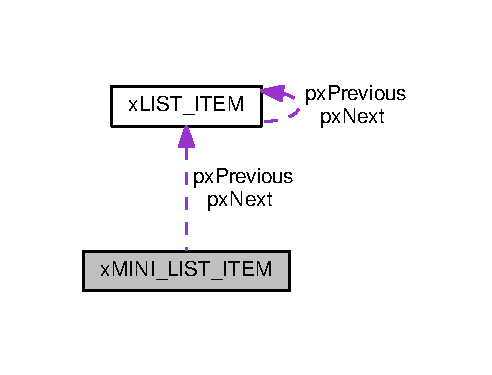
\includegraphics[width=236pt]{structx_m_i_n_i___l_i_s_t___i_t_e_m__coll__graph}
\end{center}
\end{figure}
\subsection*{Public Attributes}
\begin{DoxyCompactItemize}
\item 
\hyperlink{list_8h_a3611bd5d5d87cb26ac1dc7a4852b94a0}{list\+F\+I\+R\+S\+T\+\_\+\+L\+I\+S\+T\+\_\+\+I\+T\+E\+M\+\_\+\+I\+N\+T\+E\+G\+R\+I\+T\+Y\+\_\+\+C\+H\+E\+C\+K\+\_\+\+V\+A\+L\+UE} \hyperlink{list_8h_a2d5de557c5561c8980d1bf51d87d8cba}{config\+L\+I\+S\+T\+\_\+\+V\+O\+L\+A\+T\+I\+LE} \hyperlink{portmacro_8h_aa69c48c6e902ce54f70886e6573c92a9}{Tick\+Type\+\_\+t} \hyperlink{structx_m_i_n_i___l_i_s_t___i_t_e_m_aae79c54ac1efa30959e68604cc23b29e}{x\+Item\+Value}
\item 
struct \hyperlink{structx_l_i_s_t___i_t_e_m}{x\+L\+I\+S\+T\+\_\+\+I\+T\+EM} $\ast$\hyperlink{list_8h_a2d5de557c5561c8980d1bf51d87d8cba}{config\+L\+I\+S\+T\+\_\+\+V\+O\+L\+A\+T\+I\+LE} \hyperlink{structx_m_i_n_i___l_i_s_t___i_t_e_m_aa7ae770b0f10daeb9ac76c6f7dd5608e}{px\+Next}
\item 
struct \hyperlink{structx_l_i_s_t___i_t_e_m}{x\+L\+I\+S\+T\+\_\+\+I\+T\+EM} $\ast$\hyperlink{list_8h_a2d5de557c5561c8980d1bf51d87d8cba}{config\+L\+I\+S\+T\+\_\+\+V\+O\+L\+A\+T\+I\+LE} \hyperlink{structx_m_i_n_i___l_i_s_t___i_t_e_m_a732c666bb97560eb1b094a2c411269ab}{px\+Previous}
\end{DoxyCompactItemize}


\subsection{Detailed Description}


Definition at line 193 of file list.\+h.



\subsection{Member Data Documentation}
\index{x\+M\+I\+N\+I\+\_\+\+L\+I\+S\+T\+\_\+\+I\+T\+EM@{x\+M\+I\+N\+I\+\_\+\+L\+I\+S\+T\+\_\+\+I\+T\+EM}!px\+Next@{px\+Next}}
\index{px\+Next@{px\+Next}!x\+M\+I\+N\+I\+\_\+\+L\+I\+S\+T\+\_\+\+I\+T\+EM@{x\+M\+I\+N\+I\+\_\+\+L\+I\+S\+T\+\_\+\+I\+T\+EM}}
\subsubsection[{\texorpdfstring{px\+Next}{pxNext}}]{\setlength{\rightskip}{0pt plus 5cm}struct {\bf x\+L\+I\+S\+T\+\_\+\+I\+T\+EM}$\ast$ {\bf config\+L\+I\+S\+T\+\_\+\+V\+O\+L\+A\+T\+I\+LE} x\+M\+I\+N\+I\+\_\+\+L\+I\+S\+T\+\_\+\+I\+T\+E\+M\+::px\+Next}\hypertarget{structx_m_i_n_i___l_i_s_t___i_t_e_m_aa7ae770b0f10daeb9ac76c6f7dd5608e}{}\label{structx_m_i_n_i___l_i_s_t___i_t_e_m_aa7ae770b0f10daeb9ac76c6f7dd5608e}


Definition at line 197 of file list.\+h.

\index{x\+M\+I\+N\+I\+\_\+\+L\+I\+S\+T\+\_\+\+I\+T\+EM@{x\+M\+I\+N\+I\+\_\+\+L\+I\+S\+T\+\_\+\+I\+T\+EM}!px\+Previous@{px\+Previous}}
\index{px\+Previous@{px\+Previous}!x\+M\+I\+N\+I\+\_\+\+L\+I\+S\+T\+\_\+\+I\+T\+EM@{x\+M\+I\+N\+I\+\_\+\+L\+I\+S\+T\+\_\+\+I\+T\+EM}}
\subsubsection[{\texorpdfstring{px\+Previous}{pxPrevious}}]{\setlength{\rightskip}{0pt plus 5cm}struct {\bf x\+L\+I\+S\+T\+\_\+\+I\+T\+EM}$\ast$ {\bf config\+L\+I\+S\+T\+\_\+\+V\+O\+L\+A\+T\+I\+LE} x\+M\+I\+N\+I\+\_\+\+L\+I\+S\+T\+\_\+\+I\+T\+E\+M\+::px\+Previous}\hypertarget{structx_m_i_n_i___l_i_s_t___i_t_e_m_a732c666bb97560eb1b094a2c411269ab}{}\label{structx_m_i_n_i___l_i_s_t___i_t_e_m_a732c666bb97560eb1b094a2c411269ab}


Definition at line 198 of file list.\+h.

\index{x\+M\+I\+N\+I\+\_\+\+L\+I\+S\+T\+\_\+\+I\+T\+EM@{x\+M\+I\+N\+I\+\_\+\+L\+I\+S\+T\+\_\+\+I\+T\+EM}!x\+Item\+Value@{x\+Item\+Value}}
\index{x\+Item\+Value@{x\+Item\+Value}!x\+M\+I\+N\+I\+\_\+\+L\+I\+S\+T\+\_\+\+I\+T\+EM@{x\+M\+I\+N\+I\+\_\+\+L\+I\+S\+T\+\_\+\+I\+T\+EM}}
\subsubsection[{\texorpdfstring{x\+Item\+Value}{xItemValue}}]{\setlength{\rightskip}{0pt plus 5cm}{\bf list\+F\+I\+R\+S\+T\+\_\+\+L\+I\+S\+T\+\_\+\+I\+T\+E\+M\+\_\+\+I\+N\+T\+E\+G\+R\+I\+T\+Y\+\_\+\+C\+H\+E\+C\+K\+\_\+\+V\+A\+L\+UE} {\bf config\+L\+I\+S\+T\+\_\+\+V\+O\+L\+A\+T\+I\+LE} {\bf Tick\+Type\+\_\+t} x\+M\+I\+N\+I\+\_\+\+L\+I\+S\+T\+\_\+\+I\+T\+E\+M\+::x\+Item\+Value}\hypertarget{structx_m_i_n_i___l_i_s_t___i_t_e_m_aae79c54ac1efa30959e68604cc23b29e}{}\label{structx_m_i_n_i___l_i_s_t___i_t_e_m_aae79c54ac1efa30959e68604cc23b29e}


Definition at line 196 of file list.\+h.



The documentation for this struct was generated from the following file\+:\begin{DoxyCompactItemize}
\item 
/home/telemetria/git/workspaces/tinoc2\+\_\+firmware\+\_\+freertos/\+R\+T\+O\+S\+Demo/\+Source/\+Free\+R\+T\+O\+S\+\_\+\+Source/include/\hyperlink{list_8h}{list.\+h}\end{DoxyCompactItemize}

\hypertarget{structx_s_t_a_t_i_c___e_v_e_n_t___g_r_o_u_p}{}\section{x\+S\+T\+A\+T\+I\+C\+\_\+\+E\+V\+E\+N\+T\+\_\+\+G\+R\+O\+UP Struct Reference}
\label{structx_s_t_a_t_i_c___e_v_e_n_t___g_r_o_u_p}\index{x\+S\+T\+A\+T\+I\+C\+\_\+\+E\+V\+E\+N\+T\+\_\+\+G\+R\+O\+UP@{x\+S\+T\+A\+T\+I\+C\+\_\+\+E\+V\+E\+N\+T\+\_\+\+G\+R\+O\+UP}}


{\ttfamily \#include $<$Free\+R\+T\+O\+S.\+h$>$}



Collaboration diagram for x\+S\+T\+A\+T\+I\+C\+\_\+\+E\+V\+E\+N\+T\+\_\+\+G\+R\+O\+UP\+:\nopagebreak
\begin{figure}[H]
\begin{center}
\leavevmode
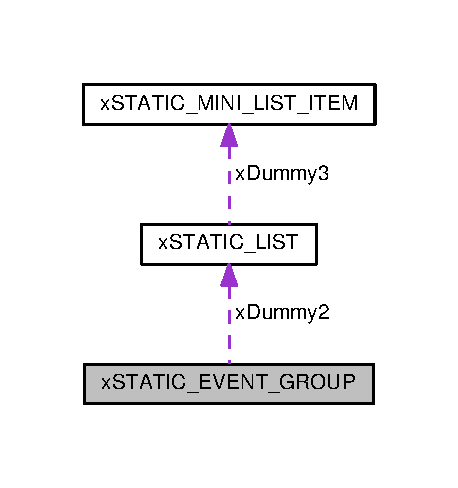
\includegraphics[width=220pt]{structx_s_t_a_t_i_c___e_v_e_n_t___g_r_o_u_p__coll__graph}
\end{center}
\end{figure}
\subsection*{Public Attributes}
\begin{DoxyCompactItemize}
\item 
\hyperlink{portmacro_8h_aa69c48c6e902ce54f70886e6573c92a9}{Tick\+Type\+\_\+t} \hyperlink{structx_s_t_a_t_i_c___e_v_e_n_t___g_r_o_u_p_a4ed0094f715dd8f79a354f42fd973fc6}{x\+Dummy1}
\item 
\hyperlink{_free_r_t_o_s_8h_a9735ad9101a2bd25f83a62089a4acee6}{Static\+List\+\_\+t} \hyperlink{structx_s_t_a_t_i_c___e_v_e_n_t___g_r_o_u_p_a17d070c972ecd0151d7505a539653551}{x\+Dummy2}
\end{DoxyCompactItemize}


\subsection{Detailed Description}


Definition at line 1012 of file Free\+R\+T\+O\+S.\+h.



\subsection{Member Data Documentation}
\index{x\+S\+T\+A\+T\+I\+C\+\_\+\+E\+V\+E\+N\+T\+\_\+\+G\+R\+O\+UP@{x\+S\+T\+A\+T\+I\+C\+\_\+\+E\+V\+E\+N\+T\+\_\+\+G\+R\+O\+UP}!x\+Dummy1@{x\+Dummy1}}
\index{x\+Dummy1@{x\+Dummy1}!x\+S\+T\+A\+T\+I\+C\+\_\+\+E\+V\+E\+N\+T\+\_\+\+G\+R\+O\+UP@{x\+S\+T\+A\+T\+I\+C\+\_\+\+E\+V\+E\+N\+T\+\_\+\+G\+R\+O\+UP}}
\subsubsection[{\texorpdfstring{x\+Dummy1}{xDummy1}}]{\setlength{\rightskip}{0pt plus 5cm}{\bf Tick\+Type\+\_\+t} x\+S\+T\+A\+T\+I\+C\+\_\+\+E\+V\+E\+N\+T\+\_\+\+G\+R\+O\+U\+P\+::x\+Dummy1}\hypertarget{structx_s_t_a_t_i_c___e_v_e_n_t___g_r_o_u_p_a4ed0094f715dd8f79a354f42fd973fc6}{}\label{structx_s_t_a_t_i_c___e_v_e_n_t___g_r_o_u_p_a4ed0094f715dd8f79a354f42fd973fc6}


Definition at line 1014 of file Free\+R\+T\+O\+S.\+h.

\index{x\+S\+T\+A\+T\+I\+C\+\_\+\+E\+V\+E\+N\+T\+\_\+\+G\+R\+O\+UP@{x\+S\+T\+A\+T\+I\+C\+\_\+\+E\+V\+E\+N\+T\+\_\+\+G\+R\+O\+UP}!x\+Dummy2@{x\+Dummy2}}
\index{x\+Dummy2@{x\+Dummy2}!x\+S\+T\+A\+T\+I\+C\+\_\+\+E\+V\+E\+N\+T\+\_\+\+G\+R\+O\+UP@{x\+S\+T\+A\+T\+I\+C\+\_\+\+E\+V\+E\+N\+T\+\_\+\+G\+R\+O\+UP}}
\subsubsection[{\texorpdfstring{x\+Dummy2}{xDummy2}}]{\setlength{\rightskip}{0pt plus 5cm}{\bf Static\+List\+\_\+t} x\+S\+T\+A\+T\+I\+C\+\_\+\+E\+V\+E\+N\+T\+\_\+\+G\+R\+O\+U\+P\+::x\+Dummy2}\hypertarget{structx_s_t_a_t_i_c___e_v_e_n_t___g_r_o_u_p_a17d070c972ecd0151d7505a539653551}{}\label{structx_s_t_a_t_i_c___e_v_e_n_t___g_r_o_u_p_a17d070c972ecd0151d7505a539653551}


Definition at line 1015 of file Free\+R\+T\+O\+S.\+h.



The documentation for this struct was generated from the following file\+:\begin{DoxyCompactItemize}
\item 
/home/telemetria/git/workspaces/tinoc2\+\_\+firmware\+\_\+freertos/\+R\+T\+O\+S\+Demo/\+Source/\+Free\+R\+T\+O\+S\+\_\+\+Source/include/\hyperlink{_free_r_t_o_s_8h}{Free\+R\+T\+O\+S.\+h}\end{DoxyCompactItemize}

\hypertarget{structx_s_t_a_t_i_c___l_i_s_t}{}\section{x\+S\+T\+A\+T\+I\+C\+\_\+\+L\+I\+ST Struct Reference}
\label{structx_s_t_a_t_i_c___l_i_s_t}\index{x\+S\+T\+A\+T\+I\+C\+\_\+\+L\+I\+ST@{x\+S\+T\+A\+T\+I\+C\+\_\+\+L\+I\+ST}}


{\ttfamily \#include $<$Free\+R\+T\+O\+S.\+h$>$}



Collaboration diagram for x\+S\+T\+A\+T\+I\+C\+\_\+\+L\+I\+ST\+:\nopagebreak
\begin{figure}[H]
\begin{center}
\leavevmode
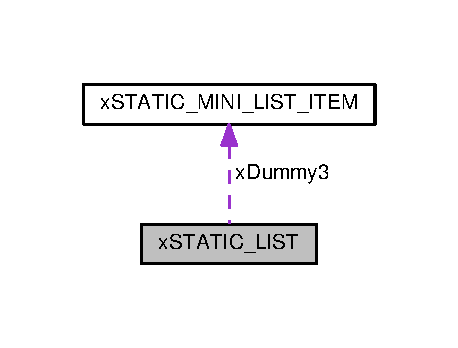
\includegraphics[width=220pt]{structx_s_t_a_t_i_c___l_i_s_t__coll__graph}
\end{center}
\end{figure}
\subsection*{Public Attributes}
\begin{DoxyCompactItemize}
\item 
\hyperlink{portmacro_8h_a646f89d4298e4f5afd522202b11cb2e6}{U\+Base\+Type\+\_\+t} \hyperlink{structx_s_t_a_t_i_c___l_i_s_t_a6d7f720dc21e3a676b885b72a945fea7}{ux\+Dummy1}
\item 
void $\ast$ \hyperlink{structx_s_t_a_t_i_c___l_i_s_t_a681e588716be5f49fe8e9eb73e8f280e}{pv\+Dummy2}
\item 
\hyperlink{_free_r_t_o_s_8h_a9097f48f4dfa56e8e01d9179462c7994}{Static\+Mini\+List\+Item\+\_\+t} \hyperlink{structx_s_t_a_t_i_c___l_i_s_t_a232545ebb5629617e0ee6ba286e37788}{x\+Dummy3}
\end{DoxyCompactItemize}


\subsection{Detailed Description}


Definition at line 890 of file Free\+R\+T\+O\+S.\+h.



\subsection{Member Data Documentation}
\index{x\+S\+T\+A\+T\+I\+C\+\_\+\+L\+I\+ST@{x\+S\+T\+A\+T\+I\+C\+\_\+\+L\+I\+ST}!pv\+Dummy2@{pv\+Dummy2}}
\index{pv\+Dummy2@{pv\+Dummy2}!x\+S\+T\+A\+T\+I\+C\+\_\+\+L\+I\+ST@{x\+S\+T\+A\+T\+I\+C\+\_\+\+L\+I\+ST}}
\subsubsection[{\texorpdfstring{pv\+Dummy2}{pvDummy2}}]{\setlength{\rightskip}{0pt plus 5cm}void$\ast$ x\+S\+T\+A\+T\+I\+C\+\_\+\+L\+I\+S\+T\+::pv\+Dummy2}\hypertarget{structx_s_t_a_t_i_c___l_i_s_t_a681e588716be5f49fe8e9eb73e8f280e}{}\label{structx_s_t_a_t_i_c___l_i_s_t_a681e588716be5f49fe8e9eb73e8f280e}


Definition at line 893 of file Free\+R\+T\+O\+S.\+h.

\index{x\+S\+T\+A\+T\+I\+C\+\_\+\+L\+I\+ST@{x\+S\+T\+A\+T\+I\+C\+\_\+\+L\+I\+ST}!ux\+Dummy1@{ux\+Dummy1}}
\index{ux\+Dummy1@{ux\+Dummy1}!x\+S\+T\+A\+T\+I\+C\+\_\+\+L\+I\+ST@{x\+S\+T\+A\+T\+I\+C\+\_\+\+L\+I\+ST}}
\subsubsection[{\texorpdfstring{ux\+Dummy1}{uxDummy1}}]{\setlength{\rightskip}{0pt plus 5cm}{\bf U\+Base\+Type\+\_\+t} x\+S\+T\+A\+T\+I\+C\+\_\+\+L\+I\+S\+T\+::ux\+Dummy1}\hypertarget{structx_s_t_a_t_i_c___l_i_s_t_a6d7f720dc21e3a676b885b72a945fea7}{}\label{structx_s_t_a_t_i_c___l_i_s_t_a6d7f720dc21e3a676b885b72a945fea7}


Definition at line 892 of file Free\+R\+T\+O\+S.\+h.

\index{x\+S\+T\+A\+T\+I\+C\+\_\+\+L\+I\+ST@{x\+S\+T\+A\+T\+I\+C\+\_\+\+L\+I\+ST}!x\+Dummy3@{x\+Dummy3}}
\index{x\+Dummy3@{x\+Dummy3}!x\+S\+T\+A\+T\+I\+C\+\_\+\+L\+I\+ST@{x\+S\+T\+A\+T\+I\+C\+\_\+\+L\+I\+ST}}
\subsubsection[{\texorpdfstring{x\+Dummy3}{xDummy3}}]{\setlength{\rightskip}{0pt plus 5cm}{\bf Static\+Mini\+List\+Item\+\_\+t} x\+S\+T\+A\+T\+I\+C\+\_\+\+L\+I\+S\+T\+::x\+Dummy3}\hypertarget{structx_s_t_a_t_i_c___l_i_s_t_a232545ebb5629617e0ee6ba286e37788}{}\label{structx_s_t_a_t_i_c___l_i_s_t_a232545ebb5629617e0ee6ba286e37788}


Definition at line 894 of file Free\+R\+T\+O\+S.\+h.



The documentation for this struct was generated from the following file\+:\begin{DoxyCompactItemize}
\item 
/home/telemetria/git/workspaces/tinoc2\+\_\+firmware\+\_\+freertos/\+R\+T\+O\+S\+Demo/\+Source/\+Free\+R\+T\+O\+S\+\_\+\+Source/include/\hyperlink{_free_r_t_o_s_8h}{Free\+R\+T\+O\+S.\+h}\end{DoxyCompactItemize}

\hypertarget{structx_s_t_a_t_i_c___l_i_s_t___i_t_e_m}{}\section{x\+S\+T\+A\+T\+I\+C\+\_\+\+L\+I\+S\+T\+\_\+\+I\+T\+EM Struct Reference}
\label{structx_s_t_a_t_i_c___l_i_s_t___i_t_e_m}\index{x\+S\+T\+A\+T\+I\+C\+\_\+\+L\+I\+S\+T\+\_\+\+I\+T\+EM@{x\+S\+T\+A\+T\+I\+C\+\_\+\+L\+I\+S\+T\+\_\+\+I\+T\+EM}}


{\ttfamily \#include $<$Free\+R\+T\+O\+S.\+h$>$}

\subsection*{Public Attributes}
\begin{DoxyCompactItemize}
\item 
\hyperlink{portmacro_8h_aa69c48c6e902ce54f70886e6573c92a9}{Tick\+Type\+\_\+t} \hyperlink{structx_s_t_a_t_i_c___l_i_s_t___i_t_e_m_abdb8e415f1bcfbba19fbf57d8d4e9438}{x\+Dummy1}
\item 
void $\ast$ \hyperlink{structx_s_t_a_t_i_c___l_i_s_t___i_t_e_m_a53c6cb2b8094f991254635d04c9be55b}{pv\+Dummy2} \mbox{[}4\mbox{]}
\end{DoxyCompactItemize}


\subsection{Detailed Description}


Definition at line 874 of file Free\+R\+T\+O\+S.\+h.



\subsection{Member Data Documentation}
\index{x\+S\+T\+A\+T\+I\+C\+\_\+\+L\+I\+S\+T\+\_\+\+I\+T\+EM@{x\+S\+T\+A\+T\+I\+C\+\_\+\+L\+I\+S\+T\+\_\+\+I\+T\+EM}!pv\+Dummy2@{pv\+Dummy2}}
\index{pv\+Dummy2@{pv\+Dummy2}!x\+S\+T\+A\+T\+I\+C\+\_\+\+L\+I\+S\+T\+\_\+\+I\+T\+EM@{x\+S\+T\+A\+T\+I\+C\+\_\+\+L\+I\+S\+T\+\_\+\+I\+T\+EM}}
\subsubsection[{\texorpdfstring{pv\+Dummy2}{pvDummy2}}]{\setlength{\rightskip}{0pt plus 5cm}void$\ast$ x\+S\+T\+A\+T\+I\+C\+\_\+\+L\+I\+S\+T\+\_\+\+I\+T\+E\+M\+::pv\+Dummy2\mbox{[}4\mbox{]}}\hypertarget{structx_s_t_a_t_i_c___l_i_s_t___i_t_e_m_a53c6cb2b8094f991254635d04c9be55b}{}\label{structx_s_t_a_t_i_c___l_i_s_t___i_t_e_m_a53c6cb2b8094f991254635d04c9be55b}


Definition at line 877 of file Free\+R\+T\+O\+S.\+h.

\index{x\+S\+T\+A\+T\+I\+C\+\_\+\+L\+I\+S\+T\+\_\+\+I\+T\+EM@{x\+S\+T\+A\+T\+I\+C\+\_\+\+L\+I\+S\+T\+\_\+\+I\+T\+EM}!x\+Dummy1@{x\+Dummy1}}
\index{x\+Dummy1@{x\+Dummy1}!x\+S\+T\+A\+T\+I\+C\+\_\+\+L\+I\+S\+T\+\_\+\+I\+T\+EM@{x\+S\+T\+A\+T\+I\+C\+\_\+\+L\+I\+S\+T\+\_\+\+I\+T\+EM}}
\subsubsection[{\texorpdfstring{x\+Dummy1}{xDummy1}}]{\setlength{\rightskip}{0pt plus 5cm}{\bf Tick\+Type\+\_\+t} x\+S\+T\+A\+T\+I\+C\+\_\+\+L\+I\+S\+T\+\_\+\+I\+T\+E\+M\+::x\+Dummy1}\hypertarget{structx_s_t_a_t_i_c___l_i_s_t___i_t_e_m_abdb8e415f1bcfbba19fbf57d8d4e9438}{}\label{structx_s_t_a_t_i_c___l_i_s_t___i_t_e_m_abdb8e415f1bcfbba19fbf57d8d4e9438}


Definition at line 876 of file Free\+R\+T\+O\+S.\+h.



The documentation for this struct was generated from the following file\+:\begin{DoxyCompactItemize}
\item 
/home/telemetria/git/workspaces/tinoc2\+\_\+firmware\+\_\+freertos/\+R\+T\+O\+S\+Demo/\+Source/\+Free\+R\+T\+O\+S\+\_\+\+Source/include/\hyperlink{_free_r_t_o_s_8h}{Free\+R\+T\+O\+S.\+h}\end{DoxyCompactItemize}

\hypertarget{structx_s_t_a_t_i_c___m_i_n_i___l_i_s_t___i_t_e_m}{}\section{x\+S\+T\+A\+T\+I\+C\+\_\+\+M\+I\+N\+I\+\_\+\+L\+I\+S\+T\+\_\+\+I\+T\+EM Struct Reference}
\label{structx_s_t_a_t_i_c___m_i_n_i___l_i_s_t___i_t_e_m}\index{x\+S\+T\+A\+T\+I\+C\+\_\+\+M\+I\+N\+I\+\_\+\+L\+I\+S\+T\+\_\+\+I\+T\+EM@{x\+S\+T\+A\+T\+I\+C\+\_\+\+M\+I\+N\+I\+\_\+\+L\+I\+S\+T\+\_\+\+I\+T\+EM}}


{\ttfamily \#include $<$Free\+R\+T\+O\+S.\+h$>$}

\subsection*{Public Attributes}
\begin{DoxyCompactItemize}
\item 
\hyperlink{portmacro_8h_aa69c48c6e902ce54f70886e6573c92a9}{Tick\+Type\+\_\+t} \hyperlink{structx_s_t_a_t_i_c___m_i_n_i___l_i_s_t___i_t_e_m_a43efd282907e8243bca29338d55dbefa}{x\+Dummy1}
\item 
void $\ast$ \hyperlink{structx_s_t_a_t_i_c___m_i_n_i___l_i_s_t___i_t_e_m_a384ac285efb6edf346f260bdc09ccac6}{pv\+Dummy2} \mbox{[}2\mbox{]}
\end{DoxyCompactItemize}


\subsection{Detailed Description}


Definition at line 882 of file Free\+R\+T\+O\+S.\+h.



\subsection{Member Data Documentation}
\index{x\+S\+T\+A\+T\+I\+C\+\_\+\+M\+I\+N\+I\+\_\+\+L\+I\+S\+T\+\_\+\+I\+T\+EM@{x\+S\+T\+A\+T\+I\+C\+\_\+\+M\+I\+N\+I\+\_\+\+L\+I\+S\+T\+\_\+\+I\+T\+EM}!pv\+Dummy2@{pv\+Dummy2}}
\index{pv\+Dummy2@{pv\+Dummy2}!x\+S\+T\+A\+T\+I\+C\+\_\+\+M\+I\+N\+I\+\_\+\+L\+I\+S\+T\+\_\+\+I\+T\+EM@{x\+S\+T\+A\+T\+I\+C\+\_\+\+M\+I\+N\+I\+\_\+\+L\+I\+S\+T\+\_\+\+I\+T\+EM}}
\subsubsection[{\texorpdfstring{pv\+Dummy2}{pvDummy2}}]{\setlength{\rightskip}{0pt plus 5cm}void$\ast$ x\+S\+T\+A\+T\+I\+C\+\_\+\+M\+I\+N\+I\+\_\+\+L\+I\+S\+T\+\_\+\+I\+T\+E\+M\+::pv\+Dummy2\mbox{[}2\mbox{]}}\hypertarget{structx_s_t_a_t_i_c___m_i_n_i___l_i_s_t___i_t_e_m_a384ac285efb6edf346f260bdc09ccac6}{}\label{structx_s_t_a_t_i_c___m_i_n_i___l_i_s_t___i_t_e_m_a384ac285efb6edf346f260bdc09ccac6}


Definition at line 885 of file Free\+R\+T\+O\+S.\+h.

\index{x\+S\+T\+A\+T\+I\+C\+\_\+\+M\+I\+N\+I\+\_\+\+L\+I\+S\+T\+\_\+\+I\+T\+EM@{x\+S\+T\+A\+T\+I\+C\+\_\+\+M\+I\+N\+I\+\_\+\+L\+I\+S\+T\+\_\+\+I\+T\+EM}!x\+Dummy1@{x\+Dummy1}}
\index{x\+Dummy1@{x\+Dummy1}!x\+S\+T\+A\+T\+I\+C\+\_\+\+M\+I\+N\+I\+\_\+\+L\+I\+S\+T\+\_\+\+I\+T\+EM@{x\+S\+T\+A\+T\+I\+C\+\_\+\+M\+I\+N\+I\+\_\+\+L\+I\+S\+T\+\_\+\+I\+T\+EM}}
\subsubsection[{\texorpdfstring{x\+Dummy1}{xDummy1}}]{\setlength{\rightskip}{0pt plus 5cm}{\bf Tick\+Type\+\_\+t} x\+S\+T\+A\+T\+I\+C\+\_\+\+M\+I\+N\+I\+\_\+\+L\+I\+S\+T\+\_\+\+I\+T\+E\+M\+::x\+Dummy1}\hypertarget{structx_s_t_a_t_i_c___m_i_n_i___l_i_s_t___i_t_e_m_a43efd282907e8243bca29338d55dbefa}{}\label{structx_s_t_a_t_i_c___m_i_n_i___l_i_s_t___i_t_e_m_a43efd282907e8243bca29338d55dbefa}


Definition at line 884 of file Free\+R\+T\+O\+S.\+h.



The documentation for this struct was generated from the following file\+:\begin{DoxyCompactItemize}
\item 
/home/telemetria/git/workspaces/tinoc2\+\_\+firmware\+\_\+freertos/\+R\+T\+O\+S\+Demo/\+Source/\+Free\+R\+T\+O\+S\+\_\+\+Source/include/\hyperlink{_free_r_t_o_s_8h}{Free\+R\+T\+O\+S.\+h}\end{DoxyCompactItemize}

\hypertarget{structx_s_t_a_t_i_c___q_u_e_u_e}{}\section{x\+S\+T\+A\+T\+I\+C\+\_\+\+Q\+U\+E\+UE Struct Reference}
\label{structx_s_t_a_t_i_c___q_u_e_u_e}\index{x\+S\+T\+A\+T\+I\+C\+\_\+\+Q\+U\+E\+UE@{x\+S\+T\+A\+T\+I\+C\+\_\+\+Q\+U\+E\+UE}}


{\ttfamily \#include $<$Free\+R\+T\+O\+S.\+h$>$}



Collaboration diagram for x\+S\+T\+A\+T\+I\+C\+\_\+\+Q\+U\+E\+UE\+:\nopagebreak
\begin{figure}[H]
\begin{center}
\leavevmode
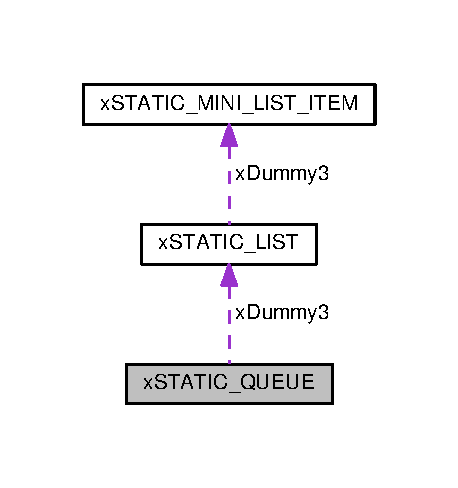
\includegraphics[width=220pt]{structx_s_t_a_t_i_c___q_u_e_u_e__coll__graph}
\end{center}
\end{figure}
\subsection*{Public Attributes}
\begin{DoxyCompactItemize}
\item 
void $\ast$ \hyperlink{structx_s_t_a_t_i_c___q_u_e_u_e_aacf22a66a8d723648995692ec77ee416}{pv\+Dummy1} \mbox{[}3\mbox{]}
\item 
\begin{tabbing}
xx\=xx\=xx\=xx\=xx\=xx\=xx\=xx\=xx\=\kill
union \{\\
\>void $\ast$ \hyperlink{structx_s_t_a_t_i_c___q_u_e_u_e_adb72a02b22a558f6fad381d65af5ac68}{pvDummy2}\\
\>\hyperlink{portmacro_8h_a646f89d4298e4f5afd522202b11cb2e6}{UBaseType\_t} \hyperlink{structx_s_t_a_t_i_c___q_u_e_u_e_ab4e6a2a0bb59ba54d05927e99afd553f}{uxDummy2}\\
\} \hyperlink{structx_s_t_a_t_i_c___q_u_e_u_e_a8a896145a0d9376a7e2713afdd782c41}{u}\\

\end{tabbing}\item 
\hyperlink{_free_r_t_o_s_8h_a9735ad9101a2bd25f83a62089a4acee6}{Static\+List\+\_\+t} \hyperlink{structx_s_t_a_t_i_c___q_u_e_u_e_add0de93e08b632124122850bcd543597}{x\+Dummy3} \mbox{[}2\mbox{]}
\item 
\hyperlink{portmacro_8h_a646f89d4298e4f5afd522202b11cb2e6}{U\+Base\+Type\+\_\+t} \hyperlink{structx_s_t_a_t_i_c___q_u_e_u_e_a502854697731754ce445f6503d14b127}{ux\+Dummy4} \mbox{[}3\mbox{]}
\item 
uint8\+\_\+t \hyperlink{structx_s_t_a_t_i_c___q_u_e_u_e_a541c5044376603540cc3c9cabcbdc5e6}{uc\+Dummy5} \mbox{[}2\mbox{]}
\end{DoxyCompactItemize}


\subsection{Detailed Description}


Definition at line 968 of file Free\+R\+T\+O\+S.\+h.



\subsection{Member Data Documentation}
\index{x\+S\+T\+A\+T\+I\+C\+\_\+\+Q\+U\+E\+UE@{x\+S\+T\+A\+T\+I\+C\+\_\+\+Q\+U\+E\+UE}!pv\+Dummy1@{pv\+Dummy1}}
\index{pv\+Dummy1@{pv\+Dummy1}!x\+S\+T\+A\+T\+I\+C\+\_\+\+Q\+U\+E\+UE@{x\+S\+T\+A\+T\+I\+C\+\_\+\+Q\+U\+E\+UE}}
\subsubsection[{\texorpdfstring{pv\+Dummy1}{pvDummy1}}]{\setlength{\rightskip}{0pt plus 5cm}void$\ast$ x\+S\+T\+A\+T\+I\+C\+\_\+\+Q\+U\+E\+U\+E\+::pv\+Dummy1\mbox{[}3\mbox{]}}\hypertarget{structx_s_t_a_t_i_c___q_u_e_u_e_aacf22a66a8d723648995692ec77ee416}{}\label{structx_s_t_a_t_i_c___q_u_e_u_e_aacf22a66a8d723648995692ec77ee416}


Definition at line 970 of file Free\+R\+T\+O\+S.\+h.

\index{x\+S\+T\+A\+T\+I\+C\+\_\+\+Q\+U\+E\+UE@{x\+S\+T\+A\+T\+I\+C\+\_\+\+Q\+U\+E\+UE}!pv\+Dummy2@{pv\+Dummy2}}
\index{pv\+Dummy2@{pv\+Dummy2}!x\+S\+T\+A\+T\+I\+C\+\_\+\+Q\+U\+E\+UE@{x\+S\+T\+A\+T\+I\+C\+\_\+\+Q\+U\+E\+UE}}
\subsubsection[{\texorpdfstring{pv\+Dummy2}{pvDummy2}}]{\setlength{\rightskip}{0pt plus 5cm}void$\ast$ x\+S\+T\+A\+T\+I\+C\+\_\+\+Q\+U\+E\+U\+E\+::pv\+Dummy2}\hypertarget{structx_s_t_a_t_i_c___q_u_e_u_e_adb72a02b22a558f6fad381d65af5ac68}{}\label{structx_s_t_a_t_i_c___q_u_e_u_e_adb72a02b22a558f6fad381d65af5ac68}


Definition at line 974 of file Free\+R\+T\+O\+S.\+h.

\index{x\+S\+T\+A\+T\+I\+C\+\_\+\+Q\+U\+E\+UE@{x\+S\+T\+A\+T\+I\+C\+\_\+\+Q\+U\+E\+UE}!u@{u}}
\index{u@{u}!x\+S\+T\+A\+T\+I\+C\+\_\+\+Q\+U\+E\+UE@{x\+S\+T\+A\+T\+I\+C\+\_\+\+Q\+U\+E\+UE}}
\subsubsection[{\texorpdfstring{u}{u}}]{\setlength{\rightskip}{0pt plus 5cm}union \{ ... \}   x\+S\+T\+A\+T\+I\+C\+\_\+\+Q\+U\+E\+U\+E\+::u}\hypertarget{structx_s_t_a_t_i_c___q_u_e_u_e_a8a896145a0d9376a7e2713afdd782c41}{}\label{structx_s_t_a_t_i_c___q_u_e_u_e_a8a896145a0d9376a7e2713afdd782c41}
\index{x\+S\+T\+A\+T\+I\+C\+\_\+\+Q\+U\+E\+UE@{x\+S\+T\+A\+T\+I\+C\+\_\+\+Q\+U\+E\+UE}!uc\+Dummy5@{uc\+Dummy5}}
\index{uc\+Dummy5@{uc\+Dummy5}!x\+S\+T\+A\+T\+I\+C\+\_\+\+Q\+U\+E\+UE@{x\+S\+T\+A\+T\+I\+C\+\_\+\+Q\+U\+E\+UE}}
\subsubsection[{\texorpdfstring{uc\+Dummy5}{ucDummy5}}]{\setlength{\rightskip}{0pt plus 5cm}uint8\+\_\+t x\+S\+T\+A\+T\+I\+C\+\_\+\+Q\+U\+E\+U\+E\+::uc\+Dummy5\mbox{[}2\mbox{]}}\hypertarget{structx_s_t_a_t_i_c___q_u_e_u_e_a541c5044376603540cc3c9cabcbdc5e6}{}\label{structx_s_t_a_t_i_c___q_u_e_u_e_a541c5044376603540cc3c9cabcbdc5e6}


Definition at line 980 of file Free\+R\+T\+O\+S.\+h.

\index{x\+S\+T\+A\+T\+I\+C\+\_\+\+Q\+U\+E\+UE@{x\+S\+T\+A\+T\+I\+C\+\_\+\+Q\+U\+E\+UE}!ux\+Dummy2@{ux\+Dummy2}}
\index{ux\+Dummy2@{ux\+Dummy2}!x\+S\+T\+A\+T\+I\+C\+\_\+\+Q\+U\+E\+UE@{x\+S\+T\+A\+T\+I\+C\+\_\+\+Q\+U\+E\+UE}}
\subsubsection[{\texorpdfstring{ux\+Dummy2}{uxDummy2}}]{\setlength{\rightskip}{0pt plus 5cm}{\bf U\+Base\+Type\+\_\+t} x\+S\+T\+A\+T\+I\+C\+\_\+\+Q\+U\+E\+U\+E\+::ux\+Dummy2}\hypertarget{structx_s_t_a_t_i_c___q_u_e_u_e_ab4e6a2a0bb59ba54d05927e99afd553f}{}\label{structx_s_t_a_t_i_c___q_u_e_u_e_ab4e6a2a0bb59ba54d05927e99afd553f}


Definition at line 975 of file Free\+R\+T\+O\+S.\+h.

\index{x\+S\+T\+A\+T\+I\+C\+\_\+\+Q\+U\+E\+UE@{x\+S\+T\+A\+T\+I\+C\+\_\+\+Q\+U\+E\+UE}!ux\+Dummy4@{ux\+Dummy4}}
\index{ux\+Dummy4@{ux\+Dummy4}!x\+S\+T\+A\+T\+I\+C\+\_\+\+Q\+U\+E\+UE@{x\+S\+T\+A\+T\+I\+C\+\_\+\+Q\+U\+E\+UE}}
\subsubsection[{\texorpdfstring{ux\+Dummy4}{uxDummy4}}]{\setlength{\rightskip}{0pt plus 5cm}{\bf U\+Base\+Type\+\_\+t} x\+S\+T\+A\+T\+I\+C\+\_\+\+Q\+U\+E\+U\+E\+::ux\+Dummy4\mbox{[}3\mbox{]}}\hypertarget{structx_s_t_a_t_i_c___q_u_e_u_e_a502854697731754ce445f6503d14b127}{}\label{structx_s_t_a_t_i_c___q_u_e_u_e_a502854697731754ce445f6503d14b127}


Definition at line 979 of file Free\+R\+T\+O\+S.\+h.

\index{x\+S\+T\+A\+T\+I\+C\+\_\+\+Q\+U\+E\+UE@{x\+S\+T\+A\+T\+I\+C\+\_\+\+Q\+U\+E\+UE}!x\+Dummy3@{x\+Dummy3}}
\index{x\+Dummy3@{x\+Dummy3}!x\+S\+T\+A\+T\+I\+C\+\_\+\+Q\+U\+E\+UE@{x\+S\+T\+A\+T\+I\+C\+\_\+\+Q\+U\+E\+UE}}
\subsubsection[{\texorpdfstring{x\+Dummy3}{xDummy3}}]{\setlength{\rightskip}{0pt plus 5cm}{\bf Static\+List\+\_\+t} x\+S\+T\+A\+T\+I\+C\+\_\+\+Q\+U\+E\+U\+E\+::x\+Dummy3\mbox{[}2\mbox{]}}\hypertarget{structx_s_t_a_t_i_c___q_u_e_u_e_add0de93e08b632124122850bcd543597}{}\label{structx_s_t_a_t_i_c___q_u_e_u_e_add0de93e08b632124122850bcd543597}


Definition at line 978 of file Free\+R\+T\+O\+S.\+h.



The documentation for this struct was generated from the following file\+:\begin{DoxyCompactItemize}
\item 
/home/telemetria/git/workspaces/tinoc2\+\_\+firmware\+\_\+freertos/\+R\+T\+O\+S\+Demo/\+Source/\+Free\+R\+T\+O\+S\+\_\+\+Source/include/\hyperlink{_free_r_t_o_s_8h}{Free\+R\+T\+O\+S.\+h}\end{DoxyCompactItemize}

\hypertarget{structx_s_t_a_t_i_c___t_c_b}{}\section{x\+S\+T\+A\+T\+I\+C\+\_\+\+T\+CB Struct Reference}
\label{structx_s_t_a_t_i_c___t_c_b}\index{x\+S\+T\+A\+T\+I\+C\+\_\+\+T\+CB@{x\+S\+T\+A\+T\+I\+C\+\_\+\+T\+CB}}


{\ttfamily \#include $<$Free\+R\+T\+O\+S.\+h$>$}



Collaboration diagram for x\+S\+T\+A\+T\+I\+C\+\_\+\+T\+CB\+:\nopagebreak
\begin{figure}[H]
\begin{center}
\leavevmode
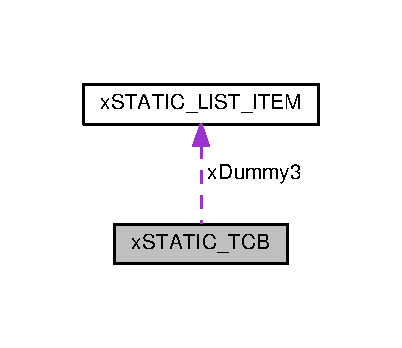
\includegraphics[width=193pt]{structx_s_t_a_t_i_c___t_c_b__coll__graph}
\end{center}
\end{figure}
\subsection*{Public Attributes}
\begin{DoxyCompactItemize}
\item 
void $\ast$ \hyperlink{structx_s_t_a_t_i_c___t_c_b_a2f66b620fdeb13f8969f27e1bbb4d1d1}{px\+Dummy1}
\item 
\hyperlink{_free_r_t_o_s_8h_a1d31bc0472385a87424518da484d9e09}{Static\+List\+Item\+\_\+t} \hyperlink{structx_s_t_a_t_i_c___t_c_b_a7f182aa8f5003494f63d975dabcb3ec1}{x\+Dummy3} \mbox{[}2\mbox{]}
\item 
\hyperlink{portmacro_8h_a646f89d4298e4f5afd522202b11cb2e6}{U\+Base\+Type\+\_\+t} \hyperlink{structx_s_t_a_t_i_c___t_c_b_ab950bb498901ef7291e49086e5a2efd0}{ux\+Dummy5}
\item 
void $\ast$ \hyperlink{structx_s_t_a_t_i_c___t_c_b_a416495e152e5caef64994f72329c60b0}{px\+Dummy6}
\item 
uint8\+\_\+t \hyperlink{structx_s_t_a_t_i_c___t_c_b_a308771ccd6723cad777695d84a0a2a30}{uc\+Dummy7} \mbox{[}\hyperlink{_free_r_t_o_s_config_8h_ac388dc4041aab6997348828eb27fc1a8}{config\+M\+A\+X\+\_\+\+T\+A\+S\+K\+\_\+\+N\+A\+M\+E\+\_\+\+L\+EN}\mbox{]}
\item 
uint32\+\_\+t \hyperlink{structx_s_t_a_t_i_c___t_c_b_ade6781276f913dcd592ee0f6cce76c7e}{ul\+Dummy18}
\item 
uint8\+\_\+t \hyperlink{structx_s_t_a_t_i_c___t_c_b_aa98151056a161f180013ae36dae0d17b}{uc\+Dummy19}
\end{DoxyCompactItemize}


\subsection{Detailed Description}


Definition at line 910 of file Free\+R\+T\+O\+S.\+h.



\subsection{Member Data Documentation}
\index{x\+S\+T\+A\+T\+I\+C\+\_\+\+T\+CB@{x\+S\+T\+A\+T\+I\+C\+\_\+\+T\+CB}!px\+Dummy1@{px\+Dummy1}}
\index{px\+Dummy1@{px\+Dummy1}!x\+S\+T\+A\+T\+I\+C\+\_\+\+T\+CB@{x\+S\+T\+A\+T\+I\+C\+\_\+\+T\+CB}}
\subsubsection[{\texorpdfstring{px\+Dummy1}{pxDummy1}}]{\setlength{\rightskip}{0pt plus 5cm}void$\ast$ x\+S\+T\+A\+T\+I\+C\+\_\+\+T\+C\+B\+::px\+Dummy1}\hypertarget{structx_s_t_a_t_i_c___t_c_b_a2f66b620fdeb13f8969f27e1bbb4d1d1}{}\label{structx_s_t_a_t_i_c___t_c_b_a2f66b620fdeb13f8969f27e1bbb4d1d1}


Definition at line 912 of file Free\+R\+T\+O\+S.\+h.

\index{x\+S\+T\+A\+T\+I\+C\+\_\+\+T\+CB@{x\+S\+T\+A\+T\+I\+C\+\_\+\+T\+CB}!px\+Dummy6@{px\+Dummy6}}
\index{px\+Dummy6@{px\+Dummy6}!x\+S\+T\+A\+T\+I\+C\+\_\+\+T\+CB@{x\+S\+T\+A\+T\+I\+C\+\_\+\+T\+CB}}
\subsubsection[{\texorpdfstring{px\+Dummy6}{pxDummy6}}]{\setlength{\rightskip}{0pt plus 5cm}void$\ast$ x\+S\+T\+A\+T\+I\+C\+\_\+\+T\+C\+B\+::px\+Dummy6}\hypertarget{structx_s_t_a_t_i_c___t_c_b_a416495e152e5caef64994f72329c60b0}{}\label{structx_s_t_a_t_i_c___t_c_b_a416495e152e5caef64994f72329c60b0}


Definition at line 918 of file Free\+R\+T\+O\+S.\+h.

\index{x\+S\+T\+A\+T\+I\+C\+\_\+\+T\+CB@{x\+S\+T\+A\+T\+I\+C\+\_\+\+T\+CB}!uc\+Dummy19@{uc\+Dummy19}}
\index{uc\+Dummy19@{uc\+Dummy19}!x\+S\+T\+A\+T\+I\+C\+\_\+\+T\+CB@{x\+S\+T\+A\+T\+I\+C\+\_\+\+T\+CB}}
\subsubsection[{\texorpdfstring{uc\+Dummy19}{ucDummy19}}]{\setlength{\rightskip}{0pt plus 5cm}uint8\+\_\+t x\+S\+T\+A\+T\+I\+C\+\_\+\+T\+C\+B\+::uc\+Dummy19}\hypertarget{structx_s_t_a_t_i_c___t_c_b_aa98151056a161f180013ae36dae0d17b}{}\label{structx_s_t_a_t_i_c___t_c_b_aa98151056a161f180013ae36dae0d17b}


Definition at line 946 of file Free\+R\+T\+O\+S.\+h.

\index{x\+S\+T\+A\+T\+I\+C\+\_\+\+T\+CB@{x\+S\+T\+A\+T\+I\+C\+\_\+\+T\+CB}!uc\+Dummy7@{uc\+Dummy7}}
\index{uc\+Dummy7@{uc\+Dummy7}!x\+S\+T\+A\+T\+I\+C\+\_\+\+T\+CB@{x\+S\+T\+A\+T\+I\+C\+\_\+\+T\+CB}}
\subsubsection[{\texorpdfstring{uc\+Dummy7}{ucDummy7}}]{\setlength{\rightskip}{0pt plus 5cm}uint8\+\_\+t x\+S\+T\+A\+T\+I\+C\+\_\+\+T\+C\+B\+::uc\+Dummy7\mbox{[}{\bf config\+M\+A\+X\+\_\+\+T\+A\+S\+K\+\_\+\+N\+A\+M\+E\+\_\+\+L\+EN}\mbox{]}}\hypertarget{structx_s_t_a_t_i_c___t_c_b_a308771ccd6723cad777695d84a0a2a30}{}\label{structx_s_t_a_t_i_c___t_c_b_a308771ccd6723cad777695d84a0a2a30}


Definition at line 919 of file Free\+R\+T\+O\+S.\+h.

\index{x\+S\+T\+A\+T\+I\+C\+\_\+\+T\+CB@{x\+S\+T\+A\+T\+I\+C\+\_\+\+T\+CB}!ul\+Dummy18@{ul\+Dummy18}}
\index{ul\+Dummy18@{ul\+Dummy18}!x\+S\+T\+A\+T\+I\+C\+\_\+\+T\+CB@{x\+S\+T\+A\+T\+I\+C\+\_\+\+T\+CB}}
\subsubsection[{\texorpdfstring{ul\+Dummy18}{ulDummy18}}]{\setlength{\rightskip}{0pt plus 5cm}uint32\+\_\+t x\+S\+T\+A\+T\+I\+C\+\_\+\+T\+C\+B\+::ul\+Dummy18}\hypertarget{structx_s_t_a_t_i_c___t_c_b_ade6781276f913dcd592ee0f6cce76c7e}{}\label{structx_s_t_a_t_i_c___t_c_b_ade6781276f913dcd592ee0f6cce76c7e}


Definition at line 945 of file Free\+R\+T\+O\+S.\+h.

\index{x\+S\+T\+A\+T\+I\+C\+\_\+\+T\+CB@{x\+S\+T\+A\+T\+I\+C\+\_\+\+T\+CB}!ux\+Dummy5@{ux\+Dummy5}}
\index{ux\+Dummy5@{ux\+Dummy5}!x\+S\+T\+A\+T\+I\+C\+\_\+\+T\+CB@{x\+S\+T\+A\+T\+I\+C\+\_\+\+T\+CB}}
\subsubsection[{\texorpdfstring{ux\+Dummy5}{uxDummy5}}]{\setlength{\rightskip}{0pt plus 5cm}{\bf U\+Base\+Type\+\_\+t} x\+S\+T\+A\+T\+I\+C\+\_\+\+T\+C\+B\+::ux\+Dummy5}\hypertarget{structx_s_t_a_t_i_c___t_c_b_ab950bb498901ef7291e49086e5a2efd0}{}\label{structx_s_t_a_t_i_c___t_c_b_ab950bb498901ef7291e49086e5a2efd0}


Definition at line 917 of file Free\+R\+T\+O\+S.\+h.

\index{x\+S\+T\+A\+T\+I\+C\+\_\+\+T\+CB@{x\+S\+T\+A\+T\+I\+C\+\_\+\+T\+CB}!x\+Dummy3@{x\+Dummy3}}
\index{x\+Dummy3@{x\+Dummy3}!x\+S\+T\+A\+T\+I\+C\+\_\+\+T\+CB@{x\+S\+T\+A\+T\+I\+C\+\_\+\+T\+CB}}
\subsubsection[{\texorpdfstring{x\+Dummy3}{xDummy3}}]{\setlength{\rightskip}{0pt plus 5cm}{\bf Static\+List\+Item\+\_\+t} x\+S\+T\+A\+T\+I\+C\+\_\+\+T\+C\+B\+::x\+Dummy3\mbox{[}2\mbox{]}}\hypertarget{structx_s_t_a_t_i_c___t_c_b_a7f182aa8f5003494f63d975dabcb3ec1}{}\label{structx_s_t_a_t_i_c___t_c_b_a7f182aa8f5003494f63d975dabcb3ec1}


Definition at line 916 of file Free\+R\+T\+O\+S.\+h.



The documentation for this struct was generated from the following file\+:\begin{DoxyCompactItemize}
\item 
/home/telemetria/git/workspaces/tinoc2\+\_\+firmware\+\_\+freertos/\+R\+T\+O\+S\+Demo/\+Source/\+Free\+R\+T\+O\+S\+\_\+\+Source/include/\hyperlink{_free_r_t_o_s_8h}{Free\+R\+T\+O\+S.\+h}\end{DoxyCompactItemize}

\hypertarget{structx_s_t_a_t_i_c___t_i_m_e_r}{}\section{x\+S\+T\+A\+T\+I\+C\+\_\+\+T\+I\+M\+ER Struct Reference}
\label{structx_s_t_a_t_i_c___t_i_m_e_r}\index{x\+S\+T\+A\+T\+I\+C\+\_\+\+T\+I\+M\+ER@{x\+S\+T\+A\+T\+I\+C\+\_\+\+T\+I\+M\+ER}}


{\ttfamily \#include $<$Free\+R\+T\+O\+S.\+h$>$}



Collaboration diagram for x\+S\+T\+A\+T\+I\+C\+\_\+\+T\+I\+M\+ER\+:\nopagebreak
\begin{figure}[H]
\begin{center}
\leavevmode
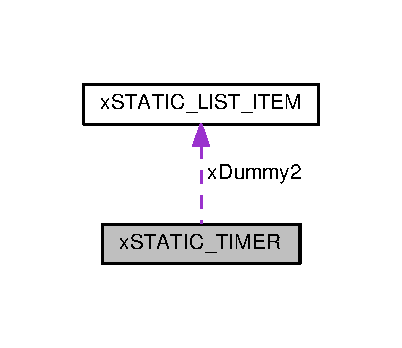
\includegraphics[width=193pt]{structx_s_t_a_t_i_c___t_i_m_e_r__coll__graph}
\end{center}
\end{figure}
\subsection*{Public Attributes}
\begin{DoxyCompactItemize}
\item 
void $\ast$ \hyperlink{structx_s_t_a_t_i_c___t_i_m_e_r_a040499298faced6032f84f3a33c785fd}{pv\+Dummy1}
\item 
\hyperlink{_free_r_t_o_s_8h_a1d31bc0472385a87424518da484d9e09}{Static\+List\+Item\+\_\+t} \hyperlink{structx_s_t_a_t_i_c___t_i_m_e_r_a622e2e596e5829c9197bb44b9009474f}{x\+Dummy2}
\item 
\hyperlink{portmacro_8h_aa69c48c6e902ce54f70886e6573c92a9}{Tick\+Type\+\_\+t} \hyperlink{structx_s_t_a_t_i_c___t_i_m_e_r_a60d582d1d0b5b9b15e8050d5ae29bc30}{x\+Dummy3}
\item 
\hyperlink{portmacro_8h_a646f89d4298e4f5afd522202b11cb2e6}{U\+Base\+Type\+\_\+t} \hyperlink{structx_s_t_a_t_i_c___t_i_m_e_r_abe61bde25ac09934004caa0222f4831b}{ux\+Dummy4}
\item 
void $\ast$ \hyperlink{structx_s_t_a_t_i_c___t_i_m_e_r_a9410b4450349079b65e2c25605913cbf}{pv\+Dummy5} \mbox{[}2\mbox{]}
\end{DoxyCompactItemize}


\subsection{Detailed Description}


Definition at line 1041 of file Free\+R\+T\+O\+S.\+h.



\subsection{Member Data Documentation}
\index{x\+S\+T\+A\+T\+I\+C\+\_\+\+T\+I\+M\+ER@{x\+S\+T\+A\+T\+I\+C\+\_\+\+T\+I\+M\+ER}!pv\+Dummy1@{pv\+Dummy1}}
\index{pv\+Dummy1@{pv\+Dummy1}!x\+S\+T\+A\+T\+I\+C\+\_\+\+T\+I\+M\+ER@{x\+S\+T\+A\+T\+I\+C\+\_\+\+T\+I\+M\+ER}}
\subsubsection[{\texorpdfstring{pv\+Dummy1}{pvDummy1}}]{\setlength{\rightskip}{0pt plus 5cm}void$\ast$ x\+S\+T\+A\+T\+I\+C\+\_\+\+T\+I\+M\+E\+R\+::pv\+Dummy1}\hypertarget{structx_s_t_a_t_i_c___t_i_m_e_r_a040499298faced6032f84f3a33c785fd}{}\label{structx_s_t_a_t_i_c___t_i_m_e_r_a040499298faced6032f84f3a33c785fd}


Definition at line 1043 of file Free\+R\+T\+O\+S.\+h.

\index{x\+S\+T\+A\+T\+I\+C\+\_\+\+T\+I\+M\+ER@{x\+S\+T\+A\+T\+I\+C\+\_\+\+T\+I\+M\+ER}!pv\+Dummy5@{pv\+Dummy5}}
\index{pv\+Dummy5@{pv\+Dummy5}!x\+S\+T\+A\+T\+I\+C\+\_\+\+T\+I\+M\+ER@{x\+S\+T\+A\+T\+I\+C\+\_\+\+T\+I\+M\+ER}}
\subsubsection[{\texorpdfstring{pv\+Dummy5}{pvDummy5}}]{\setlength{\rightskip}{0pt plus 5cm}void$\ast$ x\+S\+T\+A\+T\+I\+C\+\_\+\+T\+I\+M\+E\+R\+::pv\+Dummy5\mbox{[}2\mbox{]}}\hypertarget{structx_s_t_a_t_i_c___t_i_m_e_r_a9410b4450349079b65e2c25605913cbf}{}\label{structx_s_t_a_t_i_c___t_i_m_e_r_a9410b4450349079b65e2c25605913cbf}


Definition at line 1047 of file Free\+R\+T\+O\+S.\+h.

\index{x\+S\+T\+A\+T\+I\+C\+\_\+\+T\+I\+M\+ER@{x\+S\+T\+A\+T\+I\+C\+\_\+\+T\+I\+M\+ER}!ux\+Dummy4@{ux\+Dummy4}}
\index{ux\+Dummy4@{ux\+Dummy4}!x\+S\+T\+A\+T\+I\+C\+\_\+\+T\+I\+M\+ER@{x\+S\+T\+A\+T\+I\+C\+\_\+\+T\+I\+M\+ER}}
\subsubsection[{\texorpdfstring{ux\+Dummy4}{uxDummy4}}]{\setlength{\rightskip}{0pt plus 5cm}{\bf U\+Base\+Type\+\_\+t} x\+S\+T\+A\+T\+I\+C\+\_\+\+T\+I\+M\+E\+R\+::ux\+Dummy4}\hypertarget{structx_s_t_a_t_i_c___t_i_m_e_r_abe61bde25ac09934004caa0222f4831b}{}\label{structx_s_t_a_t_i_c___t_i_m_e_r_abe61bde25ac09934004caa0222f4831b}


Definition at line 1046 of file Free\+R\+T\+O\+S.\+h.

\index{x\+S\+T\+A\+T\+I\+C\+\_\+\+T\+I\+M\+ER@{x\+S\+T\+A\+T\+I\+C\+\_\+\+T\+I\+M\+ER}!x\+Dummy2@{x\+Dummy2}}
\index{x\+Dummy2@{x\+Dummy2}!x\+S\+T\+A\+T\+I\+C\+\_\+\+T\+I\+M\+ER@{x\+S\+T\+A\+T\+I\+C\+\_\+\+T\+I\+M\+ER}}
\subsubsection[{\texorpdfstring{x\+Dummy2}{xDummy2}}]{\setlength{\rightskip}{0pt plus 5cm}{\bf Static\+List\+Item\+\_\+t} x\+S\+T\+A\+T\+I\+C\+\_\+\+T\+I\+M\+E\+R\+::x\+Dummy2}\hypertarget{structx_s_t_a_t_i_c___t_i_m_e_r_a622e2e596e5829c9197bb44b9009474f}{}\label{structx_s_t_a_t_i_c___t_i_m_e_r_a622e2e596e5829c9197bb44b9009474f}


Definition at line 1044 of file Free\+R\+T\+O\+S.\+h.

\index{x\+S\+T\+A\+T\+I\+C\+\_\+\+T\+I\+M\+ER@{x\+S\+T\+A\+T\+I\+C\+\_\+\+T\+I\+M\+ER}!x\+Dummy3@{x\+Dummy3}}
\index{x\+Dummy3@{x\+Dummy3}!x\+S\+T\+A\+T\+I\+C\+\_\+\+T\+I\+M\+ER@{x\+S\+T\+A\+T\+I\+C\+\_\+\+T\+I\+M\+ER}}
\subsubsection[{\texorpdfstring{x\+Dummy3}{xDummy3}}]{\setlength{\rightskip}{0pt plus 5cm}{\bf Tick\+Type\+\_\+t} x\+S\+T\+A\+T\+I\+C\+\_\+\+T\+I\+M\+E\+R\+::x\+Dummy3}\hypertarget{structx_s_t_a_t_i_c___t_i_m_e_r_a60d582d1d0b5b9b15e8050d5ae29bc30}{}\label{structx_s_t_a_t_i_c___t_i_m_e_r_a60d582d1d0b5b9b15e8050d5ae29bc30}


Definition at line 1045 of file Free\+R\+T\+O\+S.\+h.



The documentation for this struct was generated from the following file\+:\begin{DoxyCompactItemize}
\item 
/home/telemetria/git/workspaces/tinoc2\+\_\+firmware\+\_\+freertos/\+R\+T\+O\+S\+Demo/\+Source/\+Free\+R\+T\+O\+S\+\_\+\+Source/include/\hyperlink{_free_r_t_o_s_8h}{Free\+R\+T\+O\+S.\+h}\end{DoxyCompactItemize}

\hypertarget{structx_t_a_s_k___p_a_r_a_m_e_t_e_r_s}{}\section{x\+T\+A\+S\+K\+\_\+\+P\+A\+R\+A\+M\+E\+T\+E\+RS Struct Reference}
\label{structx_t_a_s_k___p_a_r_a_m_e_t_e_r_s}\index{x\+T\+A\+S\+K\+\_\+\+P\+A\+R\+A\+M\+E\+T\+E\+RS@{x\+T\+A\+S\+K\+\_\+\+P\+A\+R\+A\+M\+E\+T\+E\+RS}}


{\ttfamily \#include $<$task.\+h$>$}



Collaboration diagram for x\+T\+A\+S\+K\+\_\+\+P\+A\+R\+A\+M\+E\+T\+E\+RS\+:\nopagebreak
\begin{figure}[H]
\begin{center}
\leavevmode
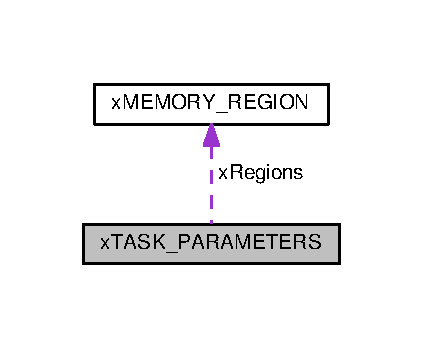
\includegraphics[width=203pt]{structx_t_a_s_k___p_a_r_a_m_e_t_e_r_s__coll__graph}
\end{center}
\end{figure}
\subsection*{Public Attributes}
\begin{DoxyCompactItemize}
\item 
\hyperlink{projdefs_8h_a9b32502ff92c255c686dacde53c1cba0}{Task\+Function\+\_\+t} \hyperlink{structx_t_a_s_k___p_a_r_a_m_e_t_e_r_s_a7527993402054565cda38251c8922880}{pv\+Task\+Code}
\item 
const char $\ast$const \hyperlink{structx_t_a_s_k___p_a_r_a_m_e_t_e_r_s_a7b3e5583acf9de8bacac572a42246459}{pc\+Name}
\item 
uint16\+\_\+t \hyperlink{structx_t_a_s_k___p_a_r_a_m_e_t_e_r_s_aa07bfb2214d78ba7a30592fa7b75af18}{us\+Stack\+Depth}
\item 
void $\ast$ \hyperlink{structx_t_a_s_k___p_a_r_a_m_e_t_e_r_s_accbb9f4de75b5b5be750198b52390c7f}{pv\+Parameters}
\item 
\hyperlink{portmacro_8h_a646f89d4298e4f5afd522202b11cb2e6}{U\+Base\+Type\+\_\+t} \hyperlink{structx_t_a_s_k___p_a_r_a_m_e_t_e_r_s_aa1aff14035db645e2bdcc85b3cdc9bab}{ux\+Priority}
\item 
\hyperlink{portmacro_8h_a84e9a8ba132feed0b2401c1f4e2ac63c}{Stack\+Type\+\_\+t} $\ast$ \hyperlink{structx_t_a_s_k___p_a_r_a_m_e_t_e_r_s_a946c525d3765369780538f9bc3f3586d}{pux\+Stack\+Buffer}
\item 
\hyperlink{task_8h_af609504de4d78ff6f71477ae47c66e51}{Memory\+Region\+\_\+t} \hyperlink{structx_t_a_s_k___p_a_r_a_m_e_t_e_r_s_ae8b97c6b7a344bf09b066b0844844d66}{x\+Regions} \mbox{[}\hyperlink{portable_8h_aca7e1a8a568a38b74cc9db10c8efebda}{port\+N\+U\+M\+\_\+\+C\+O\+N\+F\+I\+G\+U\+R\+A\+B\+L\+E\+\_\+\+R\+E\+G\+I\+O\+NS}\mbox{]}
\end{DoxyCompactItemize}


\subsection{Detailed Description}


Definition at line 154 of file task.\+h.



\subsection{Member Data Documentation}
\index{x\+T\+A\+S\+K\+\_\+\+P\+A\+R\+A\+M\+E\+T\+E\+RS@{x\+T\+A\+S\+K\+\_\+\+P\+A\+R\+A\+M\+E\+T\+E\+RS}!pc\+Name@{pc\+Name}}
\index{pc\+Name@{pc\+Name}!x\+T\+A\+S\+K\+\_\+\+P\+A\+R\+A\+M\+E\+T\+E\+RS@{x\+T\+A\+S\+K\+\_\+\+P\+A\+R\+A\+M\+E\+T\+E\+RS}}
\subsubsection[{\texorpdfstring{pc\+Name}{pcName}}]{\setlength{\rightskip}{0pt plus 5cm}const char$\ast$ const x\+T\+A\+S\+K\+\_\+\+P\+A\+R\+A\+M\+E\+T\+E\+R\+S\+::pc\+Name}\hypertarget{structx_t_a_s_k___p_a_r_a_m_e_t_e_r_s_a7b3e5583acf9de8bacac572a42246459}{}\label{structx_t_a_s_k___p_a_r_a_m_e_t_e_r_s_a7b3e5583acf9de8bacac572a42246459}


Definition at line 157 of file task.\+h.

\index{x\+T\+A\+S\+K\+\_\+\+P\+A\+R\+A\+M\+E\+T\+E\+RS@{x\+T\+A\+S\+K\+\_\+\+P\+A\+R\+A\+M\+E\+T\+E\+RS}!pux\+Stack\+Buffer@{pux\+Stack\+Buffer}}
\index{pux\+Stack\+Buffer@{pux\+Stack\+Buffer}!x\+T\+A\+S\+K\+\_\+\+P\+A\+R\+A\+M\+E\+T\+E\+RS@{x\+T\+A\+S\+K\+\_\+\+P\+A\+R\+A\+M\+E\+T\+E\+RS}}
\subsubsection[{\texorpdfstring{pux\+Stack\+Buffer}{puxStackBuffer}}]{\setlength{\rightskip}{0pt plus 5cm}{\bf Stack\+Type\+\_\+t}$\ast$ x\+T\+A\+S\+K\+\_\+\+P\+A\+R\+A\+M\+E\+T\+E\+R\+S\+::pux\+Stack\+Buffer}\hypertarget{structx_t_a_s_k___p_a_r_a_m_e_t_e_r_s_a946c525d3765369780538f9bc3f3586d}{}\label{structx_t_a_s_k___p_a_r_a_m_e_t_e_r_s_a946c525d3765369780538f9bc3f3586d}


Definition at line 161 of file task.\+h.

\index{x\+T\+A\+S\+K\+\_\+\+P\+A\+R\+A\+M\+E\+T\+E\+RS@{x\+T\+A\+S\+K\+\_\+\+P\+A\+R\+A\+M\+E\+T\+E\+RS}!pv\+Parameters@{pv\+Parameters}}
\index{pv\+Parameters@{pv\+Parameters}!x\+T\+A\+S\+K\+\_\+\+P\+A\+R\+A\+M\+E\+T\+E\+RS@{x\+T\+A\+S\+K\+\_\+\+P\+A\+R\+A\+M\+E\+T\+E\+RS}}
\subsubsection[{\texorpdfstring{pv\+Parameters}{pvParameters}}]{\setlength{\rightskip}{0pt plus 5cm}void$\ast$ x\+T\+A\+S\+K\+\_\+\+P\+A\+R\+A\+M\+E\+T\+E\+R\+S\+::pv\+Parameters}\hypertarget{structx_t_a_s_k___p_a_r_a_m_e_t_e_r_s_accbb9f4de75b5b5be750198b52390c7f}{}\label{structx_t_a_s_k___p_a_r_a_m_e_t_e_r_s_accbb9f4de75b5b5be750198b52390c7f}


Definition at line 159 of file task.\+h.

\index{x\+T\+A\+S\+K\+\_\+\+P\+A\+R\+A\+M\+E\+T\+E\+RS@{x\+T\+A\+S\+K\+\_\+\+P\+A\+R\+A\+M\+E\+T\+E\+RS}!pv\+Task\+Code@{pv\+Task\+Code}}
\index{pv\+Task\+Code@{pv\+Task\+Code}!x\+T\+A\+S\+K\+\_\+\+P\+A\+R\+A\+M\+E\+T\+E\+RS@{x\+T\+A\+S\+K\+\_\+\+P\+A\+R\+A\+M\+E\+T\+E\+RS}}
\subsubsection[{\texorpdfstring{pv\+Task\+Code}{pvTaskCode}}]{\setlength{\rightskip}{0pt plus 5cm}{\bf Task\+Function\+\_\+t} x\+T\+A\+S\+K\+\_\+\+P\+A\+R\+A\+M\+E\+T\+E\+R\+S\+::pv\+Task\+Code}\hypertarget{structx_t_a_s_k___p_a_r_a_m_e_t_e_r_s_a7527993402054565cda38251c8922880}{}\label{structx_t_a_s_k___p_a_r_a_m_e_t_e_r_s_a7527993402054565cda38251c8922880}


Definition at line 156 of file task.\+h.

\index{x\+T\+A\+S\+K\+\_\+\+P\+A\+R\+A\+M\+E\+T\+E\+RS@{x\+T\+A\+S\+K\+\_\+\+P\+A\+R\+A\+M\+E\+T\+E\+RS}!us\+Stack\+Depth@{us\+Stack\+Depth}}
\index{us\+Stack\+Depth@{us\+Stack\+Depth}!x\+T\+A\+S\+K\+\_\+\+P\+A\+R\+A\+M\+E\+T\+E\+RS@{x\+T\+A\+S\+K\+\_\+\+P\+A\+R\+A\+M\+E\+T\+E\+RS}}
\subsubsection[{\texorpdfstring{us\+Stack\+Depth}{usStackDepth}}]{\setlength{\rightskip}{0pt plus 5cm}uint16\+\_\+t x\+T\+A\+S\+K\+\_\+\+P\+A\+R\+A\+M\+E\+T\+E\+R\+S\+::us\+Stack\+Depth}\hypertarget{structx_t_a_s_k___p_a_r_a_m_e_t_e_r_s_aa07bfb2214d78ba7a30592fa7b75af18}{}\label{structx_t_a_s_k___p_a_r_a_m_e_t_e_r_s_aa07bfb2214d78ba7a30592fa7b75af18}


Definition at line 158 of file task.\+h.

\index{x\+T\+A\+S\+K\+\_\+\+P\+A\+R\+A\+M\+E\+T\+E\+RS@{x\+T\+A\+S\+K\+\_\+\+P\+A\+R\+A\+M\+E\+T\+E\+RS}!ux\+Priority@{ux\+Priority}}
\index{ux\+Priority@{ux\+Priority}!x\+T\+A\+S\+K\+\_\+\+P\+A\+R\+A\+M\+E\+T\+E\+RS@{x\+T\+A\+S\+K\+\_\+\+P\+A\+R\+A\+M\+E\+T\+E\+RS}}
\subsubsection[{\texorpdfstring{ux\+Priority}{uxPriority}}]{\setlength{\rightskip}{0pt plus 5cm}{\bf U\+Base\+Type\+\_\+t} x\+T\+A\+S\+K\+\_\+\+P\+A\+R\+A\+M\+E\+T\+E\+R\+S\+::ux\+Priority}\hypertarget{structx_t_a_s_k___p_a_r_a_m_e_t_e_r_s_aa1aff14035db645e2bdcc85b3cdc9bab}{}\label{structx_t_a_s_k___p_a_r_a_m_e_t_e_r_s_aa1aff14035db645e2bdcc85b3cdc9bab}


Definition at line 160 of file task.\+h.

\index{x\+T\+A\+S\+K\+\_\+\+P\+A\+R\+A\+M\+E\+T\+E\+RS@{x\+T\+A\+S\+K\+\_\+\+P\+A\+R\+A\+M\+E\+T\+E\+RS}!x\+Regions@{x\+Regions}}
\index{x\+Regions@{x\+Regions}!x\+T\+A\+S\+K\+\_\+\+P\+A\+R\+A\+M\+E\+T\+E\+RS@{x\+T\+A\+S\+K\+\_\+\+P\+A\+R\+A\+M\+E\+T\+E\+RS}}
\subsubsection[{\texorpdfstring{x\+Regions}{xRegions}}]{\setlength{\rightskip}{0pt plus 5cm}{\bf Memory\+Region\+\_\+t} x\+T\+A\+S\+K\+\_\+\+P\+A\+R\+A\+M\+E\+T\+E\+R\+S\+::x\+Regions\mbox{[}{\bf port\+N\+U\+M\+\_\+\+C\+O\+N\+F\+I\+G\+U\+R\+A\+B\+L\+E\+\_\+\+R\+E\+G\+I\+O\+NS}\mbox{]}}\hypertarget{structx_t_a_s_k___p_a_r_a_m_e_t_e_r_s_ae8b97c6b7a344bf09b066b0844844d66}{}\label{structx_t_a_s_k___p_a_r_a_m_e_t_e_r_s_ae8b97c6b7a344bf09b066b0844844d66}


Definition at line 162 of file task.\+h.



The documentation for this struct was generated from the following file\+:\begin{DoxyCompactItemize}
\item 
/home/telemetria/git/workspaces/tinoc2\+\_\+firmware\+\_\+freertos/\+R\+T\+O\+S\+Demo/\+Source/\+Free\+R\+T\+O\+S\+\_\+\+Source/include/\hyperlink{task_8h}{task.\+h}\end{DoxyCompactItemize}

\hypertarget{structx_t_a_s_k___s_t_a_t_u_s}{}\section{x\+T\+A\+S\+K\+\_\+\+S\+T\+A\+T\+US Struct Reference}
\label{structx_t_a_s_k___s_t_a_t_u_s}\index{x\+T\+A\+S\+K\+\_\+\+S\+T\+A\+T\+US@{x\+T\+A\+S\+K\+\_\+\+S\+T\+A\+T\+US}}


{\ttfamily \#include $<$task.\+h$>$}

\subsection*{Public Attributes}
\begin{DoxyCompactItemize}
\item 
\hyperlink{task_8h_ae95f44d4cfeb4a599c6cc258d241cb6b}{Task\+Handle\+\_\+t} \hyperlink{structx_t_a_s_k___s_t_a_t_u_s_ac57f825f365c3c64bba827285fe3c2a0}{x\+Handle}
\item 
const char $\ast$ \hyperlink{structx_t_a_s_k___s_t_a_t_u_s_ad272663e2560bd9ea088384a39ba6192}{pc\+Task\+Name}
\item 
\hyperlink{portmacro_8h_a646f89d4298e4f5afd522202b11cb2e6}{U\+Base\+Type\+\_\+t} \hyperlink{structx_t_a_s_k___s_t_a_t_u_s_acd44468ba37270b04f83d0833c098057}{x\+Task\+Number}
\item 
\hyperlink{task_8h_a1749369458e2282a22e862a619a3892c}{e\+Task\+State} \hyperlink{structx_t_a_s_k___s_t_a_t_u_s_a727e904e3afe49472b0fc6a4e96439cb}{e\+Current\+State}
\item 
\hyperlink{portmacro_8h_a646f89d4298e4f5afd522202b11cb2e6}{U\+Base\+Type\+\_\+t} \hyperlink{structx_t_a_s_k___s_t_a_t_u_s_a39df647234fc0d6de5852042a2741a94}{ux\+Current\+Priority}
\item 
\hyperlink{portmacro_8h_a646f89d4298e4f5afd522202b11cb2e6}{U\+Base\+Type\+\_\+t} \hyperlink{structx_t_a_s_k___s_t_a_t_u_s_a692f4c8957b7270f1579cdee63ff287e}{ux\+Base\+Priority}
\item 
uint32\+\_\+t \hyperlink{structx_t_a_s_k___s_t_a_t_u_s_a92ab83f4f376c255dedf8e06a78261f7}{ul\+Run\+Time\+Counter}
\item 
\hyperlink{portmacro_8h_a84e9a8ba132feed0b2401c1f4e2ac63c}{Stack\+Type\+\_\+t} $\ast$ \hyperlink{structx_t_a_s_k___s_t_a_t_u_s_a0ee59674d2cc57d3a5a29c777d5452ed}{px\+Stack\+Base}
\item 
uint16\+\_\+t \hyperlink{structx_t_a_s_k___s_t_a_t_u_s_a284892acd41bff7c319295687a95af6b}{us\+Stack\+High\+Water\+Mark}
\end{DoxyCompactItemize}


\subsection{Detailed Description}


Definition at line 167 of file task.\+h.



\subsection{Member Data Documentation}
\index{x\+T\+A\+S\+K\+\_\+\+S\+T\+A\+T\+US@{x\+T\+A\+S\+K\+\_\+\+S\+T\+A\+T\+US}!e\+Current\+State@{e\+Current\+State}}
\index{e\+Current\+State@{e\+Current\+State}!x\+T\+A\+S\+K\+\_\+\+S\+T\+A\+T\+US@{x\+T\+A\+S\+K\+\_\+\+S\+T\+A\+T\+US}}
\subsubsection[{\texorpdfstring{e\+Current\+State}{eCurrentState}}]{\setlength{\rightskip}{0pt plus 5cm}{\bf e\+Task\+State} x\+T\+A\+S\+K\+\_\+\+S\+T\+A\+T\+U\+S\+::e\+Current\+State}\hypertarget{structx_t_a_s_k___s_t_a_t_u_s_a727e904e3afe49472b0fc6a4e96439cb}{}\label{structx_t_a_s_k___s_t_a_t_u_s_a727e904e3afe49472b0fc6a4e96439cb}


Definition at line 172 of file task.\+h.

\index{x\+T\+A\+S\+K\+\_\+\+S\+T\+A\+T\+US@{x\+T\+A\+S\+K\+\_\+\+S\+T\+A\+T\+US}!pc\+Task\+Name@{pc\+Task\+Name}}
\index{pc\+Task\+Name@{pc\+Task\+Name}!x\+T\+A\+S\+K\+\_\+\+S\+T\+A\+T\+US@{x\+T\+A\+S\+K\+\_\+\+S\+T\+A\+T\+US}}
\subsubsection[{\texorpdfstring{pc\+Task\+Name}{pcTaskName}}]{\setlength{\rightskip}{0pt plus 5cm}const char$\ast$ x\+T\+A\+S\+K\+\_\+\+S\+T\+A\+T\+U\+S\+::pc\+Task\+Name}\hypertarget{structx_t_a_s_k___s_t_a_t_u_s_ad272663e2560bd9ea088384a39ba6192}{}\label{structx_t_a_s_k___s_t_a_t_u_s_ad272663e2560bd9ea088384a39ba6192}


Definition at line 170 of file task.\+h.

\index{x\+T\+A\+S\+K\+\_\+\+S\+T\+A\+T\+US@{x\+T\+A\+S\+K\+\_\+\+S\+T\+A\+T\+US}!px\+Stack\+Base@{px\+Stack\+Base}}
\index{px\+Stack\+Base@{px\+Stack\+Base}!x\+T\+A\+S\+K\+\_\+\+S\+T\+A\+T\+US@{x\+T\+A\+S\+K\+\_\+\+S\+T\+A\+T\+US}}
\subsubsection[{\texorpdfstring{px\+Stack\+Base}{pxStackBase}}]{\setlength{\rightskip}{0pt plus 5cm}{\bf Stack\+Type\+\_\+t}$\ast$ x\+T\+A\+S\+K\+\_\+\+S\+T\+A\+T\+U\+S\+::px\+Stack\+Base}\hypertarget{structx_t_a_s_k___s_t_a_t_u_s_a0ee59674d2cc57d3a5a29c777d5452ed}{}\label{structx_t_a_s_k___s_t_a_t_u_s_a0ee59674d2cc57d3a5a29c777d5452ed}


Definition at line 176 of file task.\+h.

\index{x\+T\+A\+S\+K\+\_\+\+S\+T\+A\+T\+US@{x\+T\+A\+S\+K\+\_\+\+S\+T\+A\+T\+US}!ul\+Run\+Time\+Counter@{ul\+Run\+Time\+Counter}}
\index{ul\+Run\+Time\+Counter@{ul\+Run\+Time\+Counter}!x\+T\+A\+S\+K\+\_\+\+S\+T\+A\+T\+US@{x\+T\+A\+S\+K\+\_\+\+S\+T\+A\+T\+US}}
\subsubsection[{\texorpdfstring{ul\+Run\+Time\+Counter}{ulRunTimeCounter}}]{\setlength{\rightskip}{0pt plus 5cm}uint32\+\_\+t x\+T\+A\+S\+K\+\_\+\+S\+T\+A\+T\+U\+S\+::ul\+Run\+Time\+Counter}\hypertarget{structx_t_a_s_k___s_t_a_t_u_s_a92ab83f4f376c255dedf8e06a78261f7}{}\label{structx_t_a_s_k___s_t_a_t_u_s_a92ab83f4f376c255dedf8e06a78261f7}


Definition at line 175 of file task.\+h.

\index{x\+T\+A\+S\+K\+\_\+\+S\+T\+A\+T\+US@{x\+T\+A\+S\+K\+\_\+\+S\+T\+A\+T\+US}!us\+Stack\+High\+Water\+Mark@{us\+Stack\+High\+Water\+Mark}}
\index{us\+Stack\+High\+Water\+Mark@{us\+Stack\+High\+Water\+Mark}!x\+T\+A\+S\+K\+\_\+\+S\+T\+A\+T\+US@{x\+T\+A\+S\+K\+\_\+\+S\+T\+A\+T\+US}}
\subsubsection[{\texorpdfstring{us\+Stack\+High\+Water\+Mark}{usStackHighWaterMark}}]{\setlength{\rightskip}{0pt plus 5cm}uint16\+\_\+t x\+T\+A\+S\+K\+\_\+\+S\+T\+A\+T\+U\+S\+::us\+Stack\+High\+Water\+Mark}\hypertarget{structx_t_a_s_k___s_t_a_t_u_s_a284892acd41bff7c319295687a95af6b}{}\label{structx_t_a_s_k___s_t_a_t_u_s_a284892acd41bff7c319295687a95af6b}


Definition at line 177 of file task.\+h.

\index{x\+T\+A\+S\+K\+\_\+\+S\+T\+A\+T\+US@{x\+T\+A\+S\+K\+\_\+\+S\+T\+A\+T\+US}!ux\+Base\+Priority@{ux\+Base\+Priority}}
\index{ux\+Base\+Priority@{ux\+Base\+Priority}!x\+T\+A\+S\+K\+\_\+\+S\+T\+A\+T\+US@{x\+T\+A\+S\+K\+\_\+\+S\+T\+A\+T\+US}}
\subsubsection[{\texorpdfstring{ux\+Base\+Priority}{uxBasePriority}}]{\setlength{\rightskip}{0pt plus 5cm}{\bf U\+Base\+Type\+\_\+t} x\+T\+A\+S\+K\+\_\+\+S\+T\+A\+T\+U\+S\+::ux\+Base\+Priority}\hypertarget{structx_t_a_s_k___s_t_a_t_u_s_a692f4c8957b7270f1579cdee63ff287e}{}\label{structx_t_a_s_k___s_t_a_t_u_s_a692f4c8957b7270f1579cdee63ff287e}


Definition at line 174 of file task.\+h.

\index{x\+T\+A\+S\+K\+\_\+\+S\+T\+A\+T\+US@{x\+T\+A\+S\+K\+\_\+\+S\+T\+A\+T\+US}!ux\+Current\+Priority@{ux\+Current\+Priority}}
\index{ux\+Current\+Priority@{ux\+Current\+Priority}!x\+T\+A\+S\+K\+\_\+\+S\+T\+A\+T\+US@{x\+T\+A\+S\+K\+\_\+\+S\+T\+A\+T\+US}}
\subsubsection[{\texorpdfstring{ux\+Current\+Priority}{uxCurrentPriority}}]{\setlength{\rightskip}{0pt plus 5cm}{\bf U\+Base\+Type\+\_\+t} x\+T\+A\+S\+K\+\_\+\+S\+T\+A\+T\+U\+S\+::ux\+Current\+Priority}\hypertarget{structx_t_a_s_k___s_t_a_t_u_s_a39df647234fc0d6de5852042a2741a94}{}\label{structx_t_a_s_k___s_t_a_t_u_s_a39df647234fc0d6de5852042a2741a94}


Definition at line 173 of file task.\+h.

\index{x\+T\+A\+S\+K\+\_\+\+S\+T\+A\+T\+US@{x\+T\+A\+S\+K\+\_\+\+S\+T\+A\+T\+US}!x\+Handle@{x\+Handle}}
\index{x\+Handle@{x\+Handle}!x\+T\+A\+S\+K\+\_\+\+S\+T\+A\+T\+US@{x\+T\+A\+S\+K\+\_\+\+S\+T\+A\+T\+US}}
\subsubsection[{\texorpdfstring{x\+Handle}{xHandle}}]{\setlength{\rightskip}{0pt plus 5cm}{\bf Task\+Handle\+\_\+t} x\+T\+A\+S\+K\+\_\+\+S\+T\+A\+T\+U\+S\+::x\+Handle}\hypertarget{structx_t_a_s_k___s_t_a_t_u_s_ac57f825f365c3c64bba827285fe3c2a0}{}\label{structx_t_a_s_k___s_t_a_t_u_s_ac57f825f365c3c64bba827285fe3c2a0}


Definition at line 169 of file task.\+h.

\index{x\+T\+A\+S\+K\+\_\+\+S\+T\+A\+T\+US@{x\+T\+A\+S\+K\+\_\+\+S\+T\+A\+T\+US}!x\+Task\+Number@{x\+Task\+Number}}
\index{x\+Task\+Number@{x\+Task\+Number}!x\+T\+A\+S\+K\+\_\+\+S\+T\+A\+T\+US@{x\+T\+A\+S\+K\+\_\+\+S\+T\+A\+T\+US}}
\subsubsection[{\texorpdfstring{x\+Task\+Number}{xTaskNumber}}]{\setlength{\rightskip}{0pt plus 5cm}{\bf U\+Base\+Type\+\_\+t} x\+T\+A\+S\+K\+\_\+\+S\+T\+A\+T\+U\+S\+::x\+Task\+Number}\hypertarget{structx_t_a_s_k___s_t_a_t_u_s_acd44468ba37270b04f83d0833c098057}{}\label{structx_t_a_s_k___s_t_a_t_u_s_acd44468ba37270b04f83d0833c098057}


Definition at line 171 of file task.\+h.



The documentation for this struct was generated from the following file\+:\begin{DoxyCompactItemize}
\item 
/home/telemetria/git/workspaces/tinoc2\+\_\+firmware\+\_\+freertos/\+R\+T\+O\+S\+Demo/\+Source/\+Free\+R\+T\+O\+S\+\_\+\+Source/include/\hyperlink{task_8h}{task.\+h}\end{DoxyCompactItemize}

\hypertarget{structx_t_i_m_e___o_u_t}{}\section{x\+T\+I\+M\+E\+\_\+\+O\+UT Struct Reference}
\label{structx_t_i_m_e___o_u_t}\index{x\+T\+I\+M\+E\+\_\+\+O\+UT@{x\+T\+I\+M\+E\+\_\+\+O\+UT}}


{\ttfamily \#include $<$task.\+h$>$}

\subsection*{Public Attributes}
\begin{DoxyCompactItemize}
\item 
\hyperlink{portmacro_8h_a46fb21e00ae0729d7515c0fbf2269796}{Base\+Type\+\_\+t} \hyperlink{structx_t_i_m_e___o_u_t_a9289c6f97096a9b3e3fc705d0bc5a160}{x\+Overflow\+Count}
\item 
\hyperlink{portmacro_8h_aa69c48c6e902ce54f70886e6573c92a9}{Tick\+Type\+\_\+t} \hyperlink{structx_t_i_m_e___o_u_t_a3464939ca050f7bcc6ffe0d8d3766337}{x\+Time\+On\+Entering}
\end{DoxyCompactItemize}


\subsection{Detailed Description}


Definition at line 135 of file task.\+h.



\subsection{Member Data Documentation}
\index{x\+T\+I\+M\+E\+\_\+\+O\+UT@{x\+T\+I\+M\+E\+\_\+\+O\+UT}!x\+Overflow\+Count@{x\+Overflow\+Count}}
\index{x\+Overflow\+Count@{x\+Overflow\+Count}!x\+T\+I\+M\+E\+\_\+\+O\+UT@{x\+T\+I\+M\+E\+\_\+\+O\+UT}}
\subsubsection[{\texorpdfstring{x\+Overflow\+Count}{xOverflowCount}}]{\setlength{\rightskip}{0pt plus 5cm}{\bf Base\+Type\+\_\+t} x\+T\+I\+M\+E\+\_\+\+O\+U\+T\+::x\+Overflow\+Count}\hypertarget{structx_t_i_m_e___o_u_t_a9289c6f97096a9b3e3fc705d0bc5a160}{}\label{structx_t_i_m_e___o_u_t_a9289c6f97096a9b3e3fc705d0bc5a160}


Definition at line 137 of file task.\+h.

\index{x\+T\+I\+M\+E\+\_\+\+O\+UT@{x\+T\+I\+M\+E\+\_\+\+O\+UT}!x\+Time\+On\+Entering@{x\+Time\+On\+Entering}}
\index{x\+Time\+On\+Entering@{x\+Time\+On\+Entering}!x\+T\+I\+M\+E\+\_\+\+O\+UT@{x\+T\+I\+M\+E\+\_\+\+O\+UT}}
\subsubsection[{\texorpdfstring{x\+Time\+On\+Entering}{xTimeOnEntering}}]{\setlength{\rightskip}{0pt plus 5cm}{\bf Tick\+Type\+\_\+t} x\+T\+I\+M\+E\+\_\+\+O\+U\+T\+::x\+Time\+On\+Entering}\hypertarget{structx_t_i_m_e___o_u_t_a3464939ca050f7bcc6ffe0d8d3766337}{}\label{structx_t_i_m_e___o_u_t_a3464939ca050f7bcc6ffe0d8d3766337}


Definition at line 138 of file task.\+h.



The documentation for this struct was generated from the following file\+:\begin{DoxyCompactItemize}
\item 
/home/telemetria/git/workspaces/tinoc2\+\_\+firmware\+\_\+freertos/\+R\+T\+O\+S\+Demo/\+Source/\+Free\+R\+T\+O\+S\+\_\+\+Source/include/\hyperlink{task_8h}{task.\+h}\end{DoxyCompactItemize}

\chapter{File Documentation}
\hypertarget{blocktim_8c}{}\section{/home/telemetria/git/workspaces/tinoc2\+\_\+firmware\+\_\+freertos/\+R\+T\+O\+S\+Demo/\+Source/\+Common\+\_\+\+Demo\+\_\+\+Tasks/blocktim.c File Reference}
\label{blocktim_8c}\index{/home/telemetria/git/workspaces/tinoc2\+\_\+firmware\+\_\+freertos/\+R\+T\+O\+S\+Demo/\+Source/\+Common\+\_\+\+Demo\+\_\+\+Tasks/blocktim.\+c@{/home/telemetria/git/workspaces/tinoc2\+\_\+firmware\+\_\+freertos/\+R\+T\+O\+S\+Demo/\+Source/\+Common\+\_\+\+Demo\+\_\+\+Tasks/blocktim.\+c}}
{\ttfamily \#include \char`\"{}Free\+R\+T\+O\+S.\+h\char`\"{}}\\*
{\ttfamily \#include \char`\"{}task.\+h\char`\"{}}\\*
{\ttfamily \#include \char`\"{}queue.\+h\char`\"{}}\\*
{\ttfamily \#include \char`\"{}blocktim.\+h\char`\"{}}\\*
Include dependency graph for blocktim.\+c\+:
\nopagebreak
\begin{figure}[H]
\begin{center}
\leavevmode
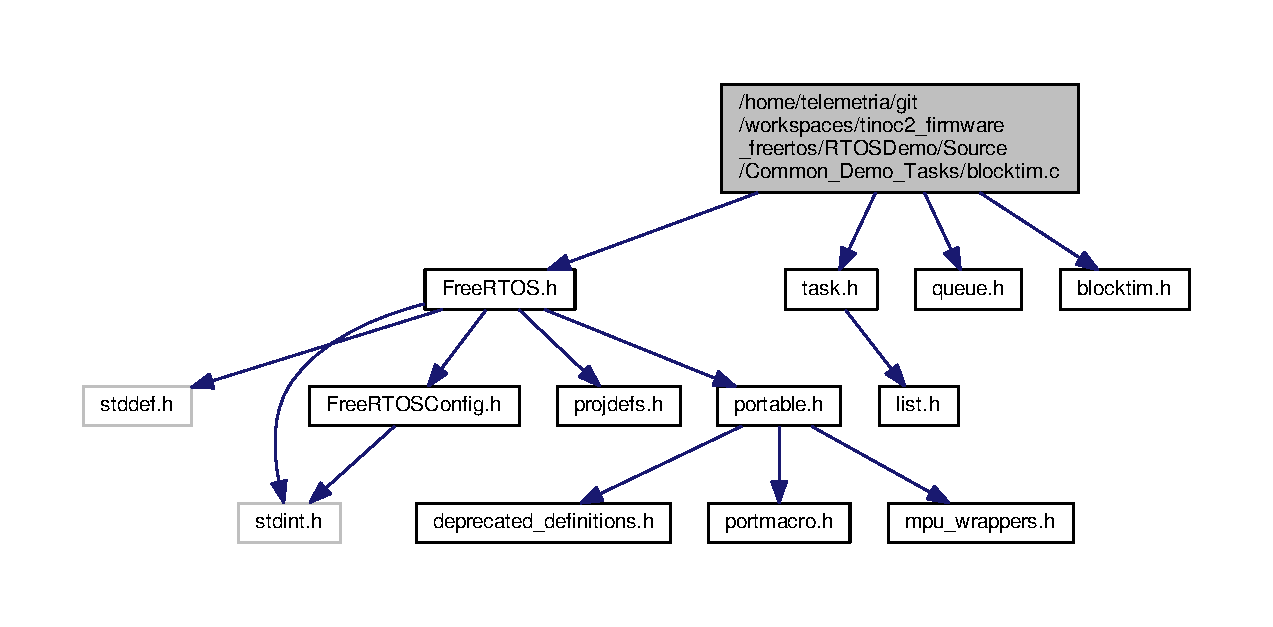
\includegraphics[width=350pt]{blocktim_8c__incl}
\end{center}
\end{figure}
\subsection*{Macros}
\begin{DoxyCompactItemize}
\item 
\#define \hyperlink{blocktim_8c_a141b4eabe1bc4e302efbc0747aaeefb3}{bkt\+P\+R\+I\+M\+A\+R\+Y\+\_\+\+P\+R\+I\+O\+R\+I\+TY}~( \hyperlink{_free_r_t_o_s_config_8h_a9a78f5ac61e6cb172dadf2a51f11db38}{config\+M\+A\+X\+\_\+\+P\+R\+I\+O\+R\+I\+T\+I\+ES} -\/ 3 )
\item 
\#define \hyperlink{blocktim_8c_a6620b6ba905c9de0a51b79672f4ea2ca}{bkt\+S\+E\+C\+O\+N\+D\+A\+R\+Y\+\_\+\+P\+R\+I\+O\+R\+I\+TY}~( \hyperlink{_free_r_t_o_s_config_8h_a9a78f5ac61e6cb172dadf2a51f11db38}{config\+M\+A\+X\+\_\+\+P\+R\+I\+O\+R\+I\+T\+I\+ES} -\/ 4 )
\item 
\#define \hyperlink{blocktim_8c_a3274df45a8be2cf211aea1d48025f071}{bkt\+Q\+U\+E\+U\+E\+\_\+\+L\+E\+N\+G\+TH}~( 5 )
\item 
\#define \hyperlink{blocktim_8c_aef5793343e5bba1e8055d61cdd255285}{bkt\+S\+H\+O\+R\+T\+\_\+\+W\+A\+IT}~\hyperlink{projdefs_8h_a353d0f62b82a402cb3db63706c81ec3f}{pd\+M\+S\+\_\+\+T\+O\+\_\+\+T\+I\+C\+KS}( ( \hyperlink{portmacro_8h_aa69c48c6e902ce54f70886e6573c92a9}{Tick\+Type\+\_\+t} ) 20 )
\item 
\#define \hyperlink{blocktim_8c_a31c09013f5ddf5a0667559a024d14a31}{bkt\+P\+R\+I\+M\+A\+R\+Y\+\_\+\+B\+L\+O\+C\+K\+\_\+\+T\+I\+ME}~( 10 )
\item 
\#define \hyperlink{blocktim_8c_a58ac1b1446b077d8bbb50531519e8808}{bkt\+A\+L\+L\+O\+W\+A\+B\+L\+E\+\_\+\+M\+A\+R\+G\+IN}~( 15 )
\item 
\#define \hyperlink{blocktim_8c_ac335943ddd482d15914cda41a4134ba1}{bkt\+T\+I\+M\+E\+\_\+\+T\+O\+\_\+\+B\+L\+O\+CK}~( 175 )
\item 
\#define \hyperlink{blocktim_8c_a5c6fdccf6ea138c2a09d200ea1431233}{bkt\+D\+O\+N\+T\+\_\+\+B\+L\+O\+CK}~( ( \hyperlink{portmacro_8h_aa69c48c6e902ce54f70886e6573c92a9}{Tick\+Type\+\_\+t} ) 0 )
\item 
\#define \hyperlink{blocktim_8c_ab8d6ee6a31954d35f5065538040f22be}{bkt\+R\+U\+N\+\_\+\+I\+N\+D\+I\+C\+A\+T\+OR}~( ( \hyperlink{portmacro_8h_a646f89d4298e4f5afd522202b11cb2e6}{U\+Base\+Type\+\_\+t} ) 0x55 )
\item 
\#define \hyperlink{blocktim_8c_a05c75ff9029ba3f0ab5bde9196f1e873}{config\+T\+I\+M\+E\+R\+\_\+\+T\+A\+S\+K\+\_\+\+P\+R\+I\+O\+R\+I\+TY}~( \hyperlink{_free_r_t_o_s_config_8h_a9a78f5ac61e6cb172dadf2a51f11db38}{config\+M\+A\+X\+\_\+\+P\+R\+I\+O\+R\+I\+T\+I\+ES} -\/ 1 )
\end{DoxyCompactItemize}
\subsection*{Functions}
\begin{DoxyCompactItemize}
\item 
static void \hyperlink{blocktim_8c_a2d16e8ca11170673dbcb90fd222d2b68}{v\+Primary\+Block\+Time\+Test\+Task} (void $\ast$pv\+Parameters)
\item 
static void \hyperlink{blocktim_8c_a4d6fcd2ddb4ec8a0aec94e8d7ebad08f}{v\+Secondary\+Block\+Time\+Test\+Task} (void $\ast$pv\+Parameters)
\item 
static void \hyperlink{blocktim_8c_aeeb5eca5aa3a749ab69b6426a78369fb}{prv\+Basic\+Delay\+Tests} (void)
\item 
void \hyperlink{blocktim_8c_a7e292a5580d071b0ed41ffa6c72a3918}{v\+Create\+Block\+Time\+Tasks} (void)
\item 
\hyperlink{portmacro_8h_a46fb21e00ae0729d7515c0fbf2269796}{Base\+Type\+\_\+t} \hyperlink{blocktim_8c_a224728c508501d2868005b78fb7dd0fc}{x\+Are\+Block\+Time\+Test\+Tasks\+Still\+Running} (void)
\end{DoxyCompactItemize}
\subsection*{Variables}
\begin{DoxyCompactItemize}
\item 
static \hyperlink{queue_8h_aaf19d499892a4ce1409326ece00f5264}{Queue\+Handle\+\_\+t} \hyperlink{blocktim_8c_ab50f695ae5f879d1ad7fff65e5dc2e7e}{x\+Test\+Queue}
\item 
static \hyperlink{task_8h_ae95f44d4cfeb4a599c6cc258d241cb6b}{Task\+Handle\+\_\+t} \hyperlink{blocktim_8c_ad86b70779c856daf9b5616511311b162}{x\+Secondary}
\item 
static volatile \hyperlink{portmacro_8h_a46fb21e00ae0729d7515c0fbf2269796}{Base\+Type\+\_\+t} \hyperlink{blocktim_8c_a87c82db51c7380bf462ae0fbd5612895}{x\+Primary\+Cycles} = 0
\item 
static volatile \hyperlink{portmacro_8h_a46fb21e00ae0729d7515c0fbf2269796}{Base\+Type\+\_\+t} \hyperlink{blocktim_8c_a0a7b8b4fcbe7aaea7f90272d1da0c92b}{x\+Secondary\+Cycles} = 0
\item 
static volatile \hyperlink{portmacro_8h_a46fb21e00ae0729d7515c0fbf2269796}{Base\+Type\+\_\+t} \hyperlink{blocktim_8c_a7d608f051774754fa525a0b7481cec3a}{x\+Error\+Occurred} = \hyperlink{projdefs_8h_aa56260e937e7e203026707e5ba944273}{pd\+F\+A\+L\+SE}
\item 
static volatile \hyperlink{portmacro_8h_a646f89d4298e4f5afd522202b11cb2e6}{U\+Base\+Type\+\_\+t} \hyperlink{blocktim_8c_ab463c5e1f292e47cd689b9f153fcb068}{x\+Run\+Indicator}
\end{DoxyCompactItemize}


\subsection{Macro Definition Documentation}
\index{blocktim.\+c@{blocktim.\+c}!bkt\+A\+L\+L\+O\+W\+A\+B\+L\+E\+\_\+\+M\+A\+R\+G\+IN@{bkt\+A\+L\+L\+O\+W\+A\+B\+L\+E\+\_\+\+M\+A\+R\+G\+IN}}
\index{bkt\+A\+L\+L\+O\+W\+A\+B\+L\+E\+\_\+\+M\+A\+R\+G\+IN@{bkt\+A\+L\+L\+O\+W\+A\+B\+L\+E\+\_\+\+M\+A\+R\+G\+IN}!blocktim.\+c@{blocktim.\+c}}
\subsubsection[{\texorpdfstring{bkt\+A\+L\+L\+O\+W\+A\+B\+L\+E\+\_\+\+M\+A\+R\+G\+IN}{bktALLOWABLE_MARGIN}}]{\setlength{\rightskip}{0pt plus 5cm}\#define bkt\+A\+L\+L\+O\+W\+A\+B\+L\+E\+\_\+\+M\+A\+R\+G\+IN~( 15 )}\hypertarget{blocktim_8c_a58ac1b1446b077d8bbb50531519e8808}{}\label{blocktim_8c_a58ac1b1446b077d8bbb50531519e8808}


Definition at line 97 of file blocktim.\+c.

\index{blocktim.\+c@{blocktim.\+c}!bkt\+D\+O\+N\+T\+\_\+\+B\+L\+O\+CK@{bkt\+D\+O\+N\+T\+\_\+\+B\+L\+O\+CK}}
\index{bkt\+D\+O\+N\+T\+\_\+\+B\+L\+O\+CK@{bkt\+D\+O\+N\+T\+\_\+\+B\+L\+O\+CK}!blocktim.\+c@{blocktim.\+c}}
\subsubsection[{\texorpdfstring{bkt\+D\+O\+N\+T\+\_\+\+B\+L\+O\+CK}{bktDONT_BLOCK}}]{\setlength{\rightskip}{0pt plus 5cm}\#define bkt\+D\+O\+N\+T\+\_\+\+B\+L\+O\+CK~( ( {\bf Tick\+Type\+\_\+t} ) 0 )}\hypertarget{blocktim_8c_a5c6fdccf6ea138c2a09d200ea1431233}{}\label{blocktim_8c_a5c6fdccf6ea138c2a09d200ea1431233}


Definition at line 99 of file blocktim.\+c.

\index{blocktim.\+c@{blocktim.\+c}!bkt\+P\+R\+I\+M\+A\+R\+Y\+\_\+\+B\+L\+O\+C\+K\+\_\+\+T\+I\+ME@{bkt\+P\+R\+I\+M\+A\+R\+Y\+\_\+\+B\+L\+O\+C\+K\+\_\+\+T\+I\+ME}}
\index{bkt\+P\+R\+I\+M\+A\+R\+Y\+\_\+\+B\+L\+O\+C\+K\+\_\+\+T\+I\+ME@{bkt\+P\+R\+I\+M\+A\+R\+Y\+\_\+\+B\+L\+O\+C\+K\+\_\+\+T\+I\+ME}!blocktim.\+c@{blocktim.\+c}}
\subsubsection[{\texorpdfstring{bkt\+P\+R\+I\+M\+A\+R\+Y\+\_\+\+B\+L\+O\+C\+K\+\_\+\+T\+I\+ME}{bktPRIMARY_BLOCK_TIME}}]{\setlength{\rightskip}{0pt plus 5cm}\#define bkt\+P\+R\+I\+M\+A\+R\+Y\+\_\+\+B\+L\+O\+C\+K\+\_\+\+T\+I\+ME~( 10 )}\hypertarget{blocktim_8c_a31c09013f5ddf5a0667559a024d14a31}{}\label{blocktim_8c_a31c09013f5ddf5a0667559a024d14a31}


Definition at line 96 of file blocktim.\+c.

\index{blocktim.\+c@{blocktim.\+c}!bkt\+P\+R\+I\+M\+A\+R\+Y\+\_\+\+P\+R\+I\+O\+R\+I\+TY@{bkt\+P\+R\+I\+M\+A\+R\+Y\+\_\+\+P\+R\+I\+O\+R\+I\+TY}}
\index{bkt\+P\+R\+I\+M\+A\+R\+Y\+\_\+\+P\+R\+I\+O\+R\+I\+TY@{bkt\+P\+R\+I\+M\+A\+R\+Y\+\_\+\+P\+R\+I\+O\+R\+I\+TY}!blocktim.\+c@{blocktim.\+c}}
\subsubsection[{\texorpdfstring{bkt\+P\+R\+I\+M\+A\+R\+Y\+\_\+\+P\+R\+I\+O\+R\+I\+TY}{bktPRIMARY_PRIORITY}}]{\setlength{\rightskip}{0pt plus 5cm}\#define bkt\+P\+R\+I\+M\+A\+R\+Y\+\_\+\+P\+R\+I\+O\+R\+I\+TY~( {\bf config\+M\+A\+X\+\_\+\+P\+R\+I\+O\+R\+I\+T\+I\+ES} -\/ 3 )}\hypertarget{blocktim_8c_a141b4eabe1bc4e302efbc0747aaeefb3}{}\label{blocktim_8c_a141b4eabe1bc4e302efbc0747aaeefb3}


Definition at line 86 of file blocktim.\+c.

\index{blocktim.\+c@{blocktim.\+c}!bkt\+Q\+U\+E\+U\+E\+\_\+\+L\+E\+N\+G\+TH@{bkt\+Q\+U\+E\+U\+E\+\_\+\+L\+E\+N\+G\+TH}}
\index{bkt\+Q\+U\+E\+U\+E\+\_\+\+L\+E\+N\+G\+TH@{bkt\+Q\+U\+E\+U\+E\+\_\+\+L\+E\+N\+G\+TH}!blocktim.\+c@{blocktim.\+c}}
\subsubsection[{\texorpdfstring{bkt\+Q\+U\+E\+U\+E\+\_\+\+L\+E\+N\+G\+TH}{bktQUEUE_LENGTH}}]{\setlength{\rightskip}{0pt plus 5cm}\#define bkt\+Q\+U\+E\+U\+E\+\_\+\+L\+E\+N\+G\+TH~( 5 )}\hypertarget{blocktim_8c_a3274df45a8be2cf211aea1d48025f071}{}\label{blocktim_8c_a3274df45a8be2cf211aea1d48025f071}


Definition at line 94 of file blocktim.\+c.

\index{blocktim.\+c@{blocktim.\+c}!bkt\+R\+U\+N\+\_\+\+I\+N\+D\+I\+C\+A\+T\+OR@{bkt\+R\+U\+N\+\_\+\+I\+N\+D\+I\+C\+A\+T\+OR}}
\index{bkt\+R\+U\+N\+\_\+\+I\+N\+D\+I\+C\+A\+T\+OR@{bkt\+R\+U\+N\+\_\+\+I\+N\+D\+I\+C\+A\+T\+OR}!blocktim.\+c@{blocktim.\+c}}
\subsubsection[{\texorpdfstring{bkt\+R\+U\+N\+\_\+\+I\+N\+D\+I\+C\+A\+T\+OR}{bktRUN_INDICATOR}}]{\setlength{\rightskip}{0pt plus 5cm}\#define bkt\+R\+U\+N\+\_\+\+I\+N\+D\+I\+C\+A\+T\+OR~( ( {\bf U\+Base\+Type\+\_\+t} ) 0x55 )}\hypertarget{blocktim_8c_ab8d6ee6a31954d35f5065538040f22be}{}\label{blocktim_8c_ab8d6ee6a31954d35f5065538040f22be}


Definition at line 100 of file blocktim.\+c.

\index{blocktim.\+c@{blocktim.\+c}!bkt\+S\+E\+C\+O\+N\+D\+A\+R\+Y\+\_\+\+P\+R\+I\+O\+R\+I\+TY@{bkt\+S\+E\+C\+O\+N\+D\+A\+R\+Y\+\_\+\+P\+R\+I\+O\+R\+I\+TY}}
\index{bkt\+S\+E\+C\+O\+N\+D\+A\+R\+Y\+\_\+\+P\+R\+I\+O\+R\+I\+TY@{bkt\+S\+E\+C\+O\+N\+D\+A\+R\+Y\+\_\+\+P\+R\+I\+O\+R\+I\+TY}!blocktim.\+c@{blocktim.\+c}}
\subsubsection[{\texorpdfstring{bkt\+S\+E\+C\+O\+N\+D\+A\+R\+Y\+\_\+\+P\+R\+I\+O\+R\+I\+TY}{bktSECONDARY_PRIORITY}}]{\setlength{\rightskip}{0pt plus 5cm}\#define bkt\+S\+E\+C\+O\+N\+D\+A\+R\+Y\+\_\+\+P\+R\+I\+O\+R\+I\+TY~( {\bf config\+M\+A\+X\+\_\+\+P\+R\+I\+O\+R\+I\+T\+I\+ES} -\/ 4 )}\hypertarget{blocktim_8c_a6620b6ba905c9de0a51b79672f4ea2ca}{}\label{blocktim_8c_a6620b6ba905c9de0a51b79672f4ea2ca}


Definition at line 90 of file blocktim.\+c.

\index{blocktim.\+c@{blocktim.\+c}!bkt\+S\+H\+O\+R\+T\+\_\+\+W\+A\+IT@{bkt\+S\+H\+O\+R\+T\+\_\+\+W\+A\+IT}}
\index{bkt\+S\+H\+O\+R\+T\+\_\+\+W\+A\+IT@{bkt\+S\+H\+O\+R\+T\+\_\+\+W\+A\+IT}!blocktim.\+c@{blocktim.\+c}}
\subsubsection[{\texorpdfstring{bkt\+S\+H\+O\+R\+T\+\_\+\+W\+A\+IT}{bktSHORT_WAIT}}]{\setlength{\rightskip}{0pt plus 5cm}\#define bkt\+S\+H\+O\+R\+T\+\_\+\+W\+A\+IT~{\bf pd\+M\+S\+\_\+\+T\+O\+\_\+\+T\+I\+C\+KS}( ( {\bf Tick\+Type\+\_\+t} ) 20 )}\hypertarget{blocktim_8c_aef5793343e5bba1e8055d61cdd255285}{}\label{blocktim_8c_aef5793343e5bba1e8055d61cdd255285}


Definition at line 95 of file blocktim.\+c.

\index{blocktim.\+c@{blocktim.\+c}!bkt\+T\+I\+M\+E\+\_\+\+T\+O\+\_\+\+B\+L\+O\+CK@{bkt\+T\+I\+M\+E\+\_\+\+T\+O\+\_\+\+B\+L\+O\+CK}}
\index{bkt\+T\+I\+M\+E\+\_\+\+T\+O\+\_\+\+B\+L\+O\+CK@{bkt\+T\+I\+M\+E\+\_\+\+T\+O\+\_\+\+B\+L\+O\+CK}!blocktim.\+c@{blocktim.\+c}}
\subsubsection[{\texorpdfstring{bkt\+T\+I\+M\+E\+\_\+\+T\+O\+\_\+\+B\+L\+O\+CK}{bktTIME_TO_BLOCK}}]{\setlength{\rightskip}{0pt plus 5cm}\#define bkt\+T\+I\+M\+E\+\_\+\+T\+O\+\_\+\+B\+L\+O\+CK~( 175 )}\hypertarget{blocktim_8c_ac335943ddd482d15914cda41a4134ba1}{}\label{blocktim_8c_ac335943ddd482d15914cda41a4134ba1}


Definition at line 98 of file blocktim.\+c.

\index{blocktim.\+c@{blocktim.\+c}!config\+T\+I\+M\+E\+R\+\_\+\+T\+A\+S\+K\+\_\+\+P\+R\+I\+O\+R\+I\+TY@{config\+T\+I\+M\+E\+R\+\_\+\+T\+A\+S\+K\+\_\+\+P\+R\+I\+O\+R\+I\+TY}}
\index{config\+T\+I\+M\+E\+R\+\_\+\+T\+A\+S\+K\+\_\+\+P\+R\+I\+O\+R\+I\+TY@{config\+T\+I\+M\+E\+R\+\_\+\+T\+A\+S\+K\+\_\+\+P\+R\+I\+O\+R\+I\+TY}!blocktim.\+c@{blocktim.\+c}}
\subsubsection[{\texorpdfstring{config\+T\+I\+M\+E\+R\+\_\+\+T\+A\+S\+K\+\_\+\+P\+R\+I\+O\+R\+I\+TY}{configTIMER_TASK_PRIORITY}}]{\setlength{\rightskip}{0pt plus 5cm}\#define config\+T\+I\+M\+E\+R\+\_\+\+T\+A\+S\+K\+\_\+\+P\+R\+I\+O\+R\+I\+TY~( {\bf config\+M\+A\+X\+\_\+\+P\+R\+I\+O\+R\+I\+T\+I\+ES} -\/ 1 )}\hypertarget{blocktim_8c_a05c75ff9029ba3f0ab5bde9196f1e873}{}\label{blocktim_8c_a05c75ff9029ba3f0ab5bde9196f1e873}


Definition at line 105 of file blocktim.\+c.



\subsection{Function Documentation}
\index{blocktim.\+c@{blocktim.\+c}!prv\+Basic\+Delay\+Tests@{prv\+Basic\+Delay\+Tests}}
\index{prv\+Basic\+Delay\+Tests@{prv\+Basic\+Delay\+Tests}!blocktim.\+c@{blocktim.\+c}}
\subsubsection[{\texorpdfstring{prv\+Basic\+Delay\+Tests(void)}{prvBasicDelayTests(void)}}]{\setlength{\rightskip}{0pt plus 5cm}static void prv\+Basic\+Delay\+Tests (
\begin{DoxyParamCaption}
\item[{void}]{}
\end{DoxyParamCaption}
)\hspace{0.3cm}{\ttfamily [static]}}\hypertarget{blocktim_8c_aeeb5eca5aa3a749ab69b6426a78369fb}{}\label{blocktim_8c_aeeb5eca5aa3a749ab69b6426a78369fb}


Definition at line 510 of file blocktim.\+c.

\index{blocktim.\+c@{blocktim.\+c}!v\+Create\+Block\+Time\+Tasks@{v\+Create\+Block\+Time\+Tasks}}
\index{v\+Create\+Block\+Time\+Tasks@{v\+Create\+Block\+Time\+Tasks}!blocktim.\+c@{blocktim.\+c}}
\subsubsection[{\texorpdfstring{v\+Create\+Block\+Time\+Tasks(void)}{vCreateBlockTimeTasks(void)}}]{\setlength{\rightskip}{0pt plus 5cm}void v\+Create\+Block\+Time\+Tasks (
\begin{DoxyParamCaption}
\item[{void}]{}
\end{DoxyParamCaption}
)}\hypertarget{blocktim_8c_a7e292a5580d071b0ed41ffa6c72a3918}{}\label{blocktim_8c_a7e292a5580d071b0ed41ffa6c72a3918}


Definition at line 140 of file blocktim.\+c.

\index{blocktim.\+c@{blocktim.\+c}!v\+Primary\+Block\+Time\+Test\+Task@{v\+Primary\+Block\+Time\+Test\+Task}}
\index{v\+Primary\+Block\+Time\+Test\+Task@{v\+Primary\+Block\+Time\+Test\+Task}!blocktim.\+c@{blocktim.\+c}}
\subsubsection[{\texorpdfstring{v\+Primary\+Block\+Time\+Test\+Task(void $\ast$pv\+Parameters)}{vPrimaryBlockTimeTestTask(void *pvParameters)}}]{\setlength{\rightskip}{0pt plus 5cm}static void v\+Primary\+Block\+Time\+Test\+Task (
\begin{DoxyParamCaption}
\item[{void $\ast$}]{pv\+Parameters}
\end{DoxyParamCaption}
)\hspace{0.3cm}{\ttfamily [static]}}\hypertarget{blocktim_8c_a2d16e8ca11170673dbcb90fd222d2b68}{}\label{blocktim_8c_a2d16e8ca11170673dbcb90fd222d2b68}


Definition at line 162 of file blocktim.\+c.

\index{blocktim.\+c@{blocktim.\+c}!v\+Secondary\+Block\+Time\+Test\+Task@{v\+Secondary\+Block\+Time\+Test\+Task}}
\index{v\+Secondary\+Block\+Time\+Test\+Task@{v\+Secondary\+Block\+Time\+Test\+Task}!blocktim.\+c@{blocktim.\+c}}
\subsubsection[{\texorpdfstring{v\+Secondary\+Block\+Time\+Test\+Task(void $\ast$pv\+Parameters)}{vSecondaryBlockTimeTestTask(void *pvParameters)}}]{\setlength{\rightskip}{0pt plus 5cm}static void v\+Secondary\+Block\+Time\+Test\+Task (
\begin{DoxyParamCaption}
\item[{void $\ast$}]{pv\+Parameters}
\end{DoxyParamCaption}
)\hspace{0.3cm}{\ttfamily [static]}}\hypertarget{blocktim_8c_a4d6fcd2ddb4ec8a0aec94e8d7ebad08f}{}\label{blocktim_8c_a4d6fcd2ddb4ec8a0aec94e8d7ebad08f}


Definition at line 420 of file blocktim.\+c.

\index{blocktim.\+c@{blocktim.\+c}!x\+Are\+Block\+Time\+Test\+Tasks\+Still\+Running@{x\+Are\+Block\+Time\+Test\+Tasks\+Still\+Running}}
\index{x\+Are\+Block\+Time\+Test\+Tasks\+Still\+Running@{x\+Are\+Block\+Time\+Test\+Tasks\+Still\+Running}!blocktim.\+c@{blocktim.\+c}}
\subsubsection[{\texorpdfstring{x\+Are\+Block\+Time\+Test\+Tasks\+Still\+Running(void)}{xAreBlockTimeTestTasksStillRunning(void)}}]{\setlength{\rightskip}{0pt plus 5cm}{\bf Base\+Type\+\_\+t} x\+Are\+Block\+Time\+Test\+Tasks\+Still\+Running (
\begin{DoxyParamCaption}
\item[{void}]{}
\end{DoxyParamCaption}
)}\hypertarget{blocktim_8c_a224728c508501d2868005b78fb7dd0fc}{}\label{blocktim_8c_a224728c508501d2868005b78fb7dd0fc}


Definition at line 556 of file blocktim.\+c.



\subsection{Variable Documentation}
\index{blocktim.\+c@{blocktim.\+c}!x\+Error\+Occurred@{x\+Error\+Occurred}}
\index{x\+Error\+Occurred@{x\+Error\+Occurred}!blocktim.\+c@{blocktim.\+c}}
\subsubsection[{\texorpdfstring{x\+Error\+Occurred}{xErrorOccurred}}]{\setlength{\rightskip}{0pt plus 5cm}volatile {\bf Base\+Type\+\_\+t} x\+Error\+Occurred = {\bf pd\+F\+A\+L\+SE}\hspace{0.3cm}{\ttfamily [static]}}\hypertarget{blocktim_8c_a7d608f051774754fa525a0b7481cec3a}{}\label{blocktim_8c_a7d608f051774754fa525a0b7481cec3a}


Definition at line 132 of file blocktim.\+c.

\index{blocktim.\+c@{blocktim.\+c}!x\+Primary\+Cycles@{x\+Primary\+Cycles}}
\index{x\+Primary\+Cycles@{x\+Primary\+Cycles}!blocktim.\+c@{blocktim.\+c}}
\subsubsection[{\texorpdfstring{x\+Primary\+Cycles}{xPrimaryCycles}}]{\setlength{\rightskip}{0pt plus 5cm}volatile {\bf Base\+Type\+\_\+t} x\+Primary\+Cycles = 0\hspace{0.3cm}{\ttfamily [static]}}\hypertarget{blocktim_8c_a87c82db51c7380bf462ae0fbd5612895}{}\label{blocktim_8c_a87c82db51c7380bf462ae0fbd5612895}


Definition at line 131 of file blocktim.\+c.

\index{blocktim.\+c@{blocktim.\+c}!x\+Run\+Indicator@{x\+Run\+Indicator}}
\index{x\+Run\+Indicator@{x\+Run\+Indicator}!blocktim.\+c@{blocktim.\+c}}
\subsubsection[{\texorpdfstring{x\+Run\+Indicator}{xRunIndicator}}]{\setlength{\rightskip}{0pt plus 5cm}volatile {\bf U\+Base\+Type\+\_\+t} x\+Run\+Indicator\hspace{0.3cm}{\ttfamily [static]}}\hypertarget{blocktim_8c_ab463c5e1f292e47cd689b9f153fcb068}{}\label{blocktim_8c_ab463c5e1f292e47cd689b9f153fcb068}


Definition at line 136 of file blocktim.\+c.

\index{blocktim.\+c@{blocktim.\+c}!x\+Secondary@{x\+Secondary}}
\index{x\+Secondary@{x\+Secondary}!blocktim.\+c@{blocktim.\+c}}
\subsubsection[{\texorpdfstring{x\+Secondary}{xSecondary}}]{\setlength{\rightskip}{0pt plus 5cm}{\bf Task\+Handle\+\_\+t} x\+Secondary\hspace{0.3cm}{\ttfamily [static]}}\hypertarget{blocktim_8c_ad86b70779c856daf9b5616511311b162}{}\label{blocktim_8c_ad86b70779c856daf9b5616511311b162}


Definition at line 128 of file blocktim.\+c.

\index{blocktim.\+c@{blocktim.\+c}!x\+Secondary\+Cycles@{x\+Secondary\+Cycles}}
\index{x\+Secondary\+Cycles@{x\+Secondary\+Cycles}!blocktim.\+c@{blocktim.\+c}}
\subsubsection[{\texorpdfstring{x\+Secondary\+Cycles}{xSecondaryCycles}}]{\setlength{\rightskip}{0pt plus 5cm}volatile {\bf Base\+Type\+\_\+t} x\+Secondary\+Cycles = 0\hspace{0.3cm}{\ttfamily [static]}}\hypertarget{blocktim_8c_a0a7b8b4fcbe7aaea7f90272d1da0c92b}{}\label{blocktim_8c_a0a7b8b4fcbe7aaea7f90272d1da0c92b}


Definition at line 131 of file blocktim.\+c.

\index{blocktim.\+c@{blocktim.\+c}!x\+Test\+Queue@{x\+Test\+Queue}}
\index{x\+Test\+Queue@{x\+Test\+Queue}!blocktim.\+c@{blocktim.\+c}}
\subsubsection[{\texorpdfstring{x\+Test\+Queue}{xTestQueue}}]{\setlength{\rightskip}{0pt plus 5cm}{\bf Queue\+Handle\+\_\+t} x\+Test\+Queue\hspace{0.3cm}{\ttfamily [static]}}\hypertarget{blocktim_8c_ab50f695ae5f879d1ad7fff65e5dc2e7e}{}\label{blocktim_8c_ab50f695ae5f879d1ad7fff65e5dc2e7e}


Definition at line 124 of file blocktim.\+c.


\hypertarget{countsem_8c}{}\section{/home/telemetria/git/workspaces/tinoc2\+\_\+firmware\+\_\+freertos/\+R\+T\+O\+S\+Demo/\+Source/\+Common\+\_\+\+Demo\+\_\+\+Tasks/countsem.c File Reference}
\label{countsem_8c}\index{/home/telemetria/git/workspaces/tinoc2\+\_\+firmware\+\_\+freertos/\+R\+T\+O\+S\+Demo/\+Source/\+Common\+\_\+\+Demo\+\_\+\+Tasks/countsem.\+c@{/home/telemetria/git/workspaces/tinoc2\+\_\+firmware\+\_\+freertos/\+R\+T\+O\+S\+Demo/\+Source/\+Common\+\_\+\+Demo\+\_\+\+Tasks/countsem.\+c}}
{\ttfamily \#include \char`\"{}Free\+R\+T\+O\+S.\+h\char`\"{}}\\*
{\ttfamily \#include \char`\"{}task.\+h\char`\"{}}\\*
{\ttfamily \#include \char`\"{}semphr.\+h\char`\"{}}\\*
{\ttfamily \#include \char`\"{}countsem.\+h\char`\"{}}\\*
Include dependency graph for countsem.\+c\+:
\nopagebreak
\begin{figure}[H]
\begin{center}
\leavevmode
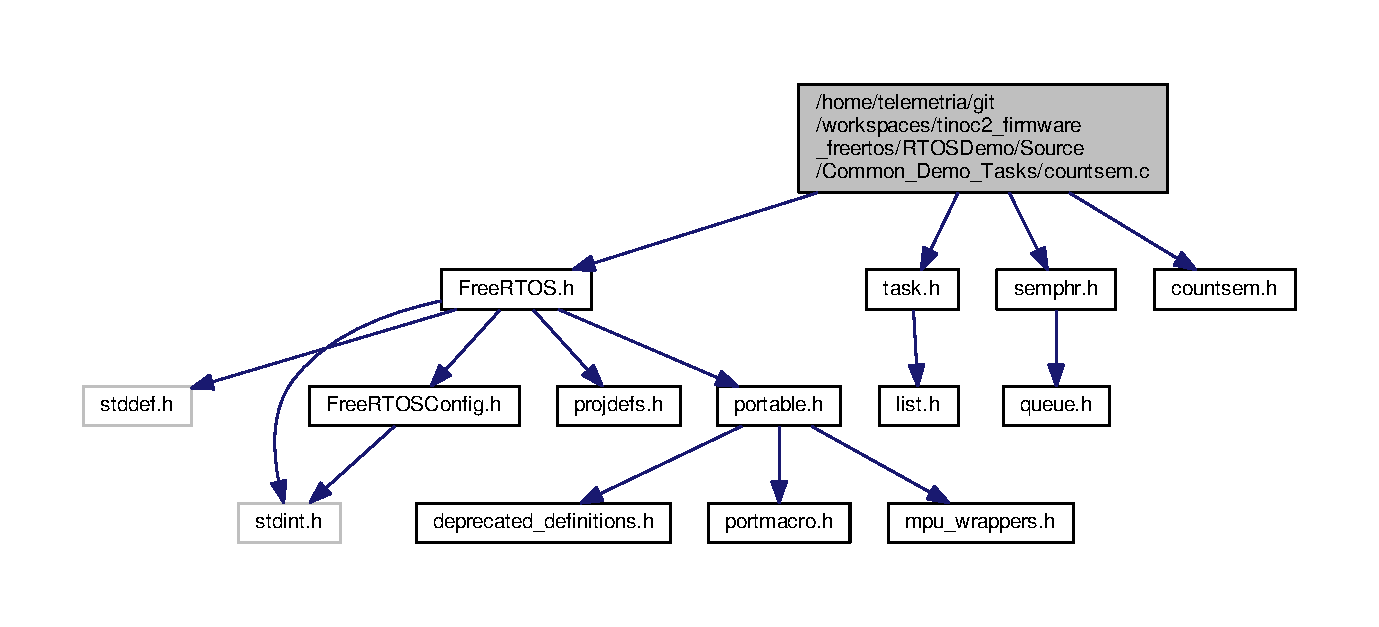
\includegraphics[width=350pt]{countsem_8c__incl}
\end{center}
\end{figure}
\subsection*{Classes}
\begin{DoxyCompactItemize}
\item 
struct \hyperlink{struct_c_o_u_n_t___s_e_m___s_t_r_u_c_t}{C\+O\+U\+N\+T\+\_\+\+S\+E\+M\+\_\+\+S\+T\+R\+U\+CT}
\end{DoxyCompactItemize}
\subsection*{Macros}
\begin{DoxyCompactItemize}
\item 
\#define \hyperlink{countsem_8c_adb434b09fb08107d0d33eddc954354f2}{count\+M\+A\+X\+\_\+\+C\+O\+U\+N\+T\+\_\+\+V\+A\+L\+UE}~( 200 )
\item 
\#define \hyperlink{countsem_8c_a65ac95e3d4f738fe0c979f264b8f2619}{count\+S\+T\+A\+R\+T\+\_\+\+A\+T\+\_\+\+M\+A\+X\+\_\+\+C\+O\+U\+NT}~( 0xaa )
\item 
\#define \hyperlink{countsem_8c_a7ea24e7d87fb8b296c3a2dd56c9c0012}{count\+S\+T\+A\+R\+T\+\_\+\+A\+T\+\_\+\+Z\+E\+RO}~( 0x55 )
\item 
\#define \hyperlink{countsem_8c_ab9bfa6a43c8e9294c9d32ebcdf61cd2e}{count\+N\+U\+M\+\_\+\+T\+E\+S\+T\+\_\+\+T\+A\+S\+KS}~( 2 )
\item 
\#define \hyperlink{countsem_8c_ae08a06fbabdb17bbd8c6d233e3f62fed}{count\+D\+O\+N\+T\+\_\+\+B\+L\+O\+CK}~( 0 )
\end{DoxyCompactItemize}
\subsection*{Typedefs}
\begin{DoxyCompactItemize}
\item 
typedef struct \hyperlink{struct_c_o_u_n_t___s_e_m___s_t_r_u_c_t}{C\+O\+U\+N\+T\+\_\+\+S\+E\+M\+\_\+\+S\+T\+R\+U\+CT} \hyperlink{countsem_8c_a7f65577ed4e66933d30c25feabc67cad}{x\+Count\+Sem\+Struct}
\end{DoxyCompactItemize}
\subsection*{Functions}
\begin{DoxyCompactItemize}
\item 
static void \hyperlink{countsem_8c_a3da2754eaeb8a4fe4945205f5ffde1b0}{prv\+Counting\+Semaphore\+Task} (void $\ast$pv\+Parameters)
\item 
static void \hyperlink{countsem_8c_a3d2925e545128b333176abfab2f89f42}{prv\+Increment\+Semaphore\+Count} (\hyperlink{semphr_8h_ad88c6df4a04beedeac782918c8a332f5}{Semaphore\+Handle\+\_\+t} x\+Semaphore, \hyperlink{portmacro_8h_a646f89d4298e4f5afd522202b11cb2e6}{U\+Base\+Type\+\_\+t} $\ast$pux\+Loop\+Counter)
\item 
static void \hyperlink{countsem_8c_a645f6f7dc2d20ef236aa2424d452da12}{prv\+Decrement\+Semaphore\+Count} (\hyperlink{semphr_8h_ad88c6df4a04beedeac782918c8a332f5}{Semaphore\+Handle\+\_\+t} x\+Semaphore, \hyperlink{portmacro_8h_a646f89d4298e4f5afd522202b11cb2e6}{U\+Base\+Type\+\_\+t} $\ast$pux\+Loop\+Counter)
\item 
void \hyperlink{countsem_8c_adb60a296dc9bf8a446919c81c1e1464d}{v\+Start\+Counting\+Semaphore\+Tasks} (void)
\item 
\hyperlink{portmacro_8h_a46fb21e00ae0729d7515c0fbf2269796}{Base\+Type\+\_\+t} \hyperlink{countsem_8c_acae097664a39290ace0006daa491c90d}{x\+Are\+Counting\+Semaphore\+Tasks\+Still\+Running} (void)
\end{DoxyCompactItemize}
\subsection*{Variables}
\begin{DoxyCompactItemize}
\item 
static volatile \hyperlink{portmacro_8h_a46fb21e00ae0729d7515c0fbf2269796}{Base\+Type\+\_\+t} \hyperlink{countsem_8c_ad88ee9dbbe7072eb80ec2240b542ad4b}{x\+Error\+Detected} = \hyperlink{projdefs_8h_aa56260e937e7e203026707e5ba944273}{pd\+F\+A\+L\+SE}
\item 
static volatile \hyperlink{countsem_8c_a7f65577ed4e66933d30c25feabc67cad}{x\+Count\+Sem\+Struct} \hyperlink{countsem_8c_a02646df01bbe5d073526ab4ed0174fa7}{x\+Parameters} \mbox{[}\hyperlink{countsem_8c_ab9bfa6a43c8e9294c9d32ebcdf61cd2e}{count\+N\+U\+M\+\_\+\+T\+E\+S\+T\+\_\+\+T\+A\+S\+KS}\mbox{]}
\end{DoxyCompactItemize}


\subsection{Macro Definition Documentation}
\index{countsem.\+c@{countsem.\+c}!count\+D\+O\+N\+T\+\_\+\+B\+L\+O\+CK@{count\+D\+O\+N\+T\+\_\+\+B\+L\+O\+CK}}
\index{count\+D\+O\+N\+T\+\_\+\+B\+L\+O\+CK@{count\+D\+O\+N\+T\+\_\+\+B\+L\+O\+CK}!countsem.\+c@{countsem.\+c}}
\subsubsection[{\texorpdfstring{count\+D\+O\+N\+T\+\_\+\+B\+L\+O\+CK}{countDONT_BLOCK}}]{\setlength{\rightskip}{0pt plus 5cm}\#define count\+D\+O\+N\+T\+\_\+\+B\+L\+O\+CK~( 0 )}\hypertarget{countsem_8c_ae08a06fbabdb17bbd8c6d233e3f62fed}{}\label{countsem_8c_ae08a06fbabdb17bbd8c6d233e3f62fed}


Definition at line 96 of file countsem.\+c.

\index{countsem.\+c@{countsem.\+c}!count\+M\+A\+X\+\_\+\+C\+O\+U\+N\+T\+\_\+\+V\+A\+L\+UE@{count\+M\+A\+X\+\_\+\+C\+O\+U\+N\+T\+\_\+\+V\+A\+L\+UE}}
\index{count\+M\+A\+X\+\_\+\+C\+O\+U\+N\+T\+\_\+\+V\+A\+L\+UE@{count\+M\+A\+X\+\_\+\+C\+O\+U\+N\+T\+\_\+\+V\+A\+L\+UE}!countsem.\+c@{countsem.\+c}}
\subsubsection[{\texorpdfstring{count\+M\+A\+X\+\_\+\+C\+O\+U\+N\+T\+\_\+\+V\+A\+L\+UE}{countMAX_COUNT_VALUE}}]{\setlength{\rightskip}{0pt plus 5cm}\#define count\+M\+A\+X\+\_\+\+C\+O\+U\+N\+T\+\_\+\+V\+A\+L\+UE~( 200 )}\hypertarget{countsem_8c_adb434b09fb08107d0d33eddc954354f2}{}\label{countsem_8c_adb434b09fb08107d0d33eddc954354f2}


Definition at line 84 of file countsem.\+c.

\index{countsem.\+c@{countsem.\+c}!count\+N\+U\+M\+\_\+\+T\+E\+S\+T\+\_\+\+T\+A\+S\+KS@{count\+N\+U\+M\+\_\+\+T\+E\+S\+T\+\_\+\+T\+A\+S\+KS}}
\index{count\+N\+U\+M\+\_\+\+T\+E\+S\+T\+\_\+\+T\+A\+S\+KS@{count\+N\+U\+M\+\_\+\+T\+E\+S\+T\+\_\+\+T\+A\+S\+KS}!countsem.\+c@{countsem.\+c}}
\subsubsection[{\texorpdfstring{count\+N\+U\+M\+\_\+\+T\+E\+S\+T\+\_\+\+T\+A\+S\+KS}{countNUM_TEST_TASKS}}]{\setlength{\rightskip}{0pt plus 5cm}\#define count\+N\+U\+M\+\_\+\+T\+E\+S\+T\+\_\+\+T\+A\+S\+KS~( 2 )}\hypertarget{countsem_8c_ab9bfa6a43c8e9294c9d32ebcdf61cd2e}{}\label{countsem_8c_ab9bfa6a43c8e9294c9d32ebcdf61cd2e}


Definition at line 95 of file countsem.\+c.

\index{countsem.\+c@{countsem.\+c}!count\+S\+T\+A\+R\+T\+\_\+\+A\+T\+\_\+\+M\+A\+X\+\_\+\+C\+O\+U\+NT@{count\+S\+T\+A\+R\+T\+\_\+\+A\+T\+\_\+\+M\+A\+X\+\_\+\+C\+O\+U\+NT}}
\index{count\+S\+T\+A\+R\+T\+\_\+\+A\+T\+\_\+\+M\+A\+X\+\_\+\+C\+O\+U\+NT@{count\+S\+T\+A\+R\+T\+\_\+\+A\+T\+\_\+\+M\+A\+X\+\_\+\+C\+O\+U\+NT}!countsem.\+c@{countsem.\+c}}
\subsubsection[{\texorpdfstring{count\+S\+T\+A\+R\+T\+\_\+\+A\+T\+\_\+\+M\+A\+X\+\_\+\+C\+O\+U\+NT}{countSTART_AT_MAX_COUNT}}]{\setlength{\rightskip}{0pt plus 5cm}\#define count\+S\+T\+A\+R\+T\+\_\+\+A\+T\+\_\+\+M\+A\+X\+\_\+\+C\+O\+U\+NT~( 0xaa )}\hypertarget{countsem_8c_a65ac95e3d4f738fe0c979f264b8f2619}{}\label{countsem_8c_a65ac95e3d4f738fe0c979f264b8f2619}


Definition at line 90 of file countsem.\+c.

\index{countsem.\+c@{countsem.\+c}!count\+S\+T\+A\+R\+T\+\_\+\+A\+T\+\_\+\+Z\+E\+RO@{count\+S\+T\+A\+R\+T\+\_\+\+A\+T\+\_\+\+Z\+E\+RO}}
\index{count\+S\+T\+A\+R\+T\+\_\+\+A\+T\+\_\+\+Z\+E\+RO@{count\+S\+T\+A\+R\+T\+\_\+\+A\+T\+\_\+\+Z\+E\+RO}!countsem.\+c@{countsem.\+c}}
\subsubsection[{\texorpdfstring{count\+S\+T\+A\+R\+T\+\_\+\+A\+T\+\_\+\+Z\+E\+RO}{countSTART_AT_ZERO}}]{\setlength{\rightskip}{0pt plus 5cm}\#define count\+S\+T\+A\+R\+T\+\_\+\+A\+T\+\_\+\+Z\+E\+RO~( 0x55 )}\hypertarget{countsem_8c_a7ea24e7d87fb8b296c3a2dd56c9c0012}{}\label{countsem_8c_a7ea24e7d87fb8b296c3a2dd56c9c0012}


Definition at line 91 of file countsem.\+c.



\subsection{Typedef Documentation}
\index{countsem.\+c@{countsem.\+c}!x\+Count\+Sem\+Struct@{x\+Count\+Sem\+Struct}}
\index{x\+Count\+Sem\+Struct@{x\+Count\+Sem\+Struct}!countsem.\+c@{countsem.\+c}}
\subsubsection[{\texorpdfstring{x\+Count\+Sem\+Struct}{xCountSemStruct}}]{\setlength{\rightskip}{0pt plus 5cm}typedef struct {\bf C\+O\+U\+N\+T\+\_\+\+S\+E\+M\+\_\+\+S\+T\+R\+U\+CT}  {\bf x\+Count\+Sem\+Struct}}\hypertarget{countsem_8c_a7f65577ed4e66933d30c25feabc67cad}{}\label{countsem_8c_a7f65577ed4e66933d30c25feabc67cad}


\subsection{Function Documentation}
\index{countsem.\+c@{countsem.\+c}!prv\+Counting\+Semaphore\+Task@{prv\+Counting\+Semaphore\+Task}}
\index{prv\+Counting\+Semaphore\+Task@{prv\+Counting\+Semaphore\+Task}!countsem.\+c@{countsem.\+c}}
\subsubsection[{\texorpdfstring{prv\+Counting\+Semaphore\+Task(void $\ast$pv\+Parameters)}{prvCountingSemaphoreTask(void *pvParameters)}}]{\setlength{\rightskip}{0pt plus 5cm}static void prv\+Counting\+Semaphore\+Task (
\begin{DoxyParamCaption}
\item[{void $\ast$}]{pv\+Parameters}
\end{DoxyParamCaption}
)\hspace{0.3cm}{\ttfamily [static]}}\hypertarget{countsem_8c_a3da2754eaeb8a4fe4945205f5ffde1b0}{}\label{countsem_8c_a3da2754eaeb8a4fe4945205f5ffde1b0}


Definition at line 258 of file countsem.\+c.

\index{countsem.\+c@{countsem.\+c}!prv\+Decrement\+Semaphore\+Count@{prv\+Decrement\+Semaphore\+Count}}
\index{prv\+Decrement\+Semaphore\+Count@{prv\+Decrement\+Semaphore\+Count}!countsem.\+c@{countsem.\+c}}
\subsubsection[{\texorpdfstring{prv\+Decrement\+Semaphore\+Count(\+Semaphore\+Handle\+\_\+t x\+Semaphore, U\+Base\+Type\+\_\+t $\ast$pux\+Loop\+Counter)}{prvDecrementSemaphoreCount(SemaphoreHandle_t xSemaphore, UBaseType_t *puxLoopCounter)}}]{\setlength{\rightskip}{0pt plus 5cm}static void prv\+Decrement\+Semaphore\+Count (
\begin{DoxyParamCaption}
\item[{{\bf Semaphore\+Handle\+\_\+t}}]{x\+Semaphore, }
\item[{{\bf U\+Base\+Type\+\_\+t} $\ast$}]{pux\+Loop\+Counter}
\end{DoxyParamCaption}
)\hspace{0.3cm}{\ttfamily [static]}}\hypertarget{countsem_8c_a645f6f7dc2d20ef236aa2424d452da12}{}\label{countsem_8c_a645f6f7dc2d20ef236aa2424d452da12}


Definition at line 181 of file countsem.\+c.

\index{countsem.\+c@{countsem.\+c}!prv\+Increment\+Semaphore\+Count@{prv\+Increment\+Semaphore\+Count}}
\index{prv\+Increment\+Semaphore\+Count@{prv\+Increment\+Semaphore\+Count}!countsem.\+c@{countsem.\+c}}
\subsubsection[{\texorpdfstring{prv\+Increment\+Semaphore\+Count(\+Semaphore\+Handle\+\_\+t x\+Semaphore, U\+Base\+Type\+\_\+t $\ast$pux\+Loop\+Counter)}{prvIncrementSemaphoreCount(SemaphoreHandle_t xSemaphore, UBaseType_t *puxLoopCounter)}}]{\setlength{\rightskip}{0pt plus 5cm}static void prv\+Increment\+Semaphore\+Count (
\begin{DoxyParamCaption}
\item[{{\bf Semaphore\+Handle\+\_\+t}}]{x\+Semaphore, }
\item[{{\bf U\+Base\+Type\+\_\+t} $\ast$}]{pux\+Loop\+Counter}
\end{DoxyParamCaption}
)\hspace{0.3cm}{\ttfamily [static]}}\hypertarget{countsem_8c_a3d2925e545128b333176abfab2f89f42}{}\label{countsem_8c_a3d2925e545128b333176abfab2f89f42}


Definition at line 220 of file countsem.\+c.

\index{countsem.\+c@{countsem.\+c}!v\+Start\+Counting\+Semaphore\+Tasks@{v\+Start\+Counting\+Semaphore\+Tasks}}
\index{v\+Start\+Counting\+Semaphore\+Tasks@{v\+Start\+Counting\+Semaphore\+Tasks}!countsem.\+c@{countsem.\+c}}
\subsubsection[{\texorpdfstring{v\+Start\+Counting\+Semaphore\+Tasks(void)}{vStartCountingSemaphoreTasks(void)}}]{\setlength{\rightskip}{0pt plus 5cm}void v\+Start\+Counting\+Semaphore\+Tasks (
\begin{DoxyParamCaption}
\item[{void}]{}
\end{DoxyParamCaption}
)}\hypertarget{countsem_8c_adb60a296dc9bf8a446919c81c1e1464d}{}\label{countsem_8c_adb60a296dc9bf8a446919c81c1e1464d}


Definition at line 149 of file countsem.\+c.

\index{countsem.\+c@{countsem.\+c}!x\+Are\+Counting\+Semaphore\+Tasks\+Still\+Running@{x\+Are\+Counting\+Semaphore\+Tasks\+Still\+Running}}
\index{x\+Are\+Counting\+Semaphore\+Tasks\+Still\+Running@{x\+Are\+Counting\+Semaphore\+Tasks\+Still\+Running}!countsem.\+c@{countsem.\+c}}
\subsubsection[{\texorpdfstring{x\+Are\+Counting\+Semaphore\+Tasks\+Still\+Running(void)}{xAreCountingSemaphoreTasksStillRunning(void)}}]{\setlength{\rightskip}{0pt plus 5cm}{\bf Base\+Type\+\_\+t} x\+Are\+Counting\+Semaphore\+Tasks\+Still\+Running (
\begin{DoxyParamCaption}
\item[{void}]{}
\end{DoxyParamCaption}
)}\hypertarget{countsem_8c_acae097664a39290ace0006daa491c90d}{}\label{countsem_8c_acae097664a39290ace0006daa491c90d}


Definition at line 296 of file countsem.\+c.



\subsection{Variable Documentation}
\index{countsem.\+c@{countsem.\+c}!x\+Error\+Detected@{x\+Error\+Detected}}
\index{x\+Error\+Detected@{x\+Error\+Detected}!countsem.\+c@{countsem.\+c}}
\subsubsection[{\texorpdfstring{x\+Error\+Detected}{xErrorDetected}}]{\setlength{\rightskip}{0pt plus 5cm}volatile {\bf Base\+Type\+\_\+t} x\+Error\+Detected = {\bf pd\+F\+A\+L\+SE}\hspace{0.3cm}{\ttfamily [static]}}\hypertarget{countsem_8c_ad88ee9dbbe7072eb80ec2240b542ad4b}{}\label{countsem_8c_ad88ee9dbbe7072eb80ec2240b542ad4b}


Definition at line 102 of file countsem.\+c.

\index{countsem.\+c@{countsem.\+c}!x\+Parameters@{x\+Parameters}}
\index{x\+Parameters@{x\+Parameters}!countsem.\+c@{countsem.\+c}}
\subsubsection[{\texorpdfstring{x\+Parameters}{xParameters}}]{\setlength{\rightskip}{0pt plus 5cm}volatile {\bf x\+Count\+Sem\+Struct} x\+Parameters\mbox{[}{\bf count\+N\+U\+M\+\_\+\+T\+E\+S\+T\+\_\+\+T\+A\+S\+KS}\mbox{]}\hspace{0.3cm}{\ttfamily [static]}}\hypertarget{countsem_8c_a02646df01bbe5d073526ab4ed0174fa7}{}\label{countsem_8c_a02646df01bbe5d073526ab4ed0174fa7}


Definition at line 145 of file countsem.\+c.


\hypertarget{blocktim_8h}{}\section{/home/telemetria/git/workspaces/tinoc2\+\_\+firmware\+\_\+freertos/\+R\+T\+O\+S\+Demo/\+Source/\+Common\+\_\+\+Demo\+\_\+\+Tasks/include/blocktim.h File Reference}
\label{blocktim_8h}\index{/home/telemetria/git/workspaces/tinoc2\+\_\+firmware\+\_\+freertos/\+R\+T\+O\+S\+Demo/\+Source/\+Common\+\_\+\+Demo\+\_\+\+Tasks/include/blocktim.\+h@{/home/telemetria/git/workspaces/tinoc2\+\_\+firmware\+\_\+freertos/\+R\+T\+O\+S\+Demo/\+Source/\+Common\+\_\+\+Demo\+\_\+\+Tasks/include/blocktim.\+h}}
This graph shows which files directly or indirectly include this file\+:
\nopagebreak
\begin{figure}[H]
\begin{center}
\leavevmode
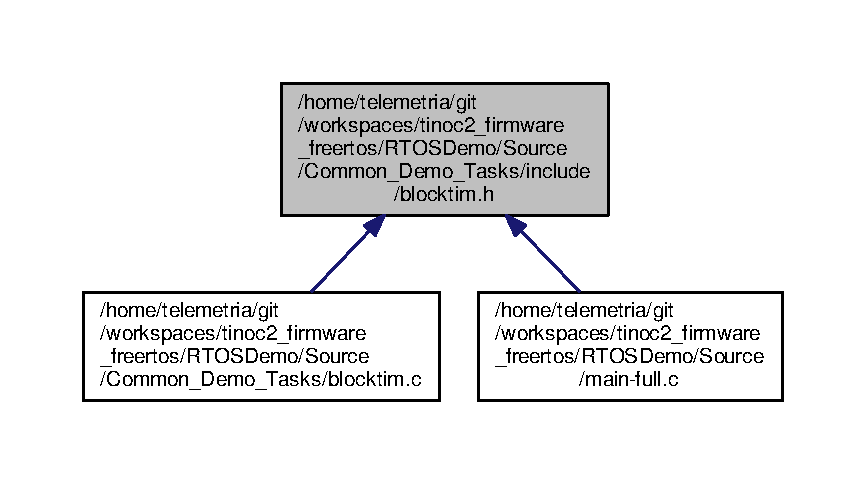
\includegraphics[width=350pt]{blocktim_8h__dep__incl}
\end{center}
\end{figure}
\subsection*{Functions}
\begin{DoxyCompactItemize}
\item 
void \hyperlink{blocktim_8h_a7e292a5580d071b0ed41ffa6c72a3918}{v\+Create\+Block\+Time\+Tasks} (void)
\item 
\hyperlink{portmacro_8h_a46fb21e00ae0729d7515c0fbf2269796}{Base\+Type\+\_\+t} \hyperlink{blocktim_8h_a224728c508501d2868005b78fb7dd0fc}{x\+Are\+Block\+Time\+Test\+Tasks\+Still\+Running} (void)
\end{DoxyCompactItemize}


\subsection{Function Documentation}
\index{blocktim.\+h@{blocktim.\+h}!v\+Create\+Block\+Time\+Tasks@{v\+Create\+Block\+Time\+Tasks}}
\index{v\+Create\+Block\+Time\+Tasks@{v\+Create\+Block\+Time\+Tasks}!blocktim.\+h@{blocktim.\+h}}
\subsubsection[{\texorpdfstring{v\+Create\+Block\+Time\+Tasks(void)}{vCreateBlockTimeTasks(void)}}]{\setlength{\rightskip}{0pt plus 5cm}void v\+Create\+Block\+Time\+Tasks (
\begin{DoxyParamCaption}
\item[{void}]{}
\end{DoxyParamCaption}
)}\hypertarget{blocktim_8h_a7e292a5580d071b0ed41ffa6c72a3918}{}\label{blocktim_8h_a7e292a5580d071b0ed41ffa6c72a3918}


Definition at line 140 of file blocktim.\+c.

\index{blocktim.\+h@{blocktim.\+h}!x\+Are\+Block\+Time\+Test\+Tasks\+Still\+Running@{x\+Are\+Block\+Time\+Test\+Tasks\+Still\+Running}}
\index{x\+Are\+Block\+Time\+Test\+Tasks\+Still\+Running@{x\+Are\+Block\+Time\+Test\+Tasks\+Still\+Running}!blocktim.\+h@{blocktim.\+h}}
\subsubsection[{\texorpdfstring{x\+Are\+Block\+Time\+Test\+Tasks\+Still\+Running(void)}{xAreBlockTimeTestTasksStillRunning(void)}}]{\setlength{\rightskip}{0pt plus 5cm}{\bf Base\+Type\+\_\+t} x\+Are\+Block\+Time\+Test\+Tasks\+Still\+Running (
\begin{DoxyParamCaption}
\item[{void}]{}
\end{DoxyParamCaption}
)}\hypertarget{blocktim_8h_a224728c508501d2868005b78fb7dd0fc}{}\label{blocktim_8h_a224728c508501d2868005b78fb7dd0fc}


Definition at line 556 of file blocktim.\+c.


\hypertarget{countsem_8h}{}\section{/home/telemetria/git/workspaces/tinoc2\+\_\+firmware\+\_\+freertos/\+R\+T\+O\+S\+Demo/\+Source/\+Common\+\_\+\+Demo\+\_\+\+Tasks/include/countsem.h File Reference}
\label{countsem_8h}\index{/home/telemetria/git/workspaces/tinoc2\+\_\+firmware\+\_\+freertos/\+R\+T\+O\+S\+Demo/\+Source/\+Common\+\_\+\+Demo\+\_\+\+Tasks/include/countsem.\+h@{/home/telemetria/git/workspaces/tinoc2\+\_\+firmware\+\_\+freertos/\+R\+T\+O\+S\+Demo/\+Source/\+Common\+\_\+\+Demo\+\_\+\+Tasks/include/countsem.\+h}}
This graph shows which files directly or indirectly include this file\+:
\nopagebreak
\begin{figure}[H]
\begin{center}
\leavevmode
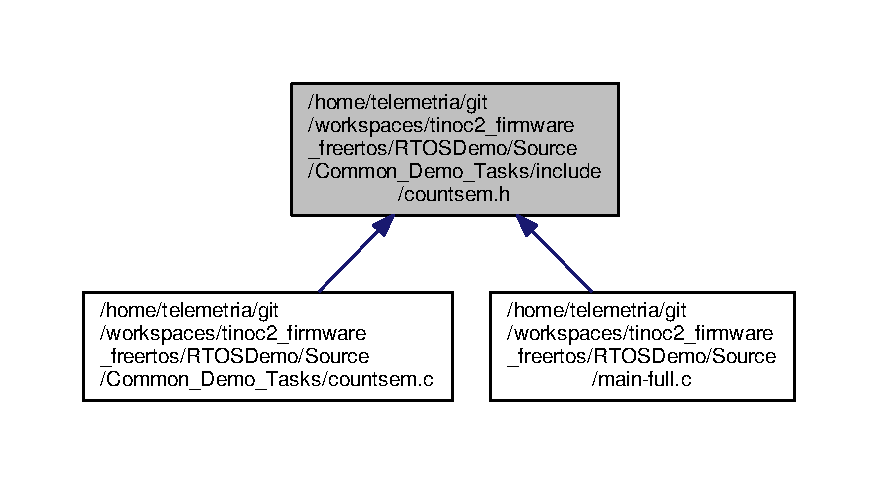
\includegraphics[width=350pt]{countsem_8h__dep__incl}
\end{center}
\end{figure}
\subsection*{Functions}
\begin{DoxyCompactItemize}
\item 
void \hyperlink{countsem_8h_adb60a296dc9bf8a446919c81c1e1464d}{v\+Start\+Counting\+Semaphore\+Tasks} (void)
\item 
\hyperlink{portmacro_8h_a46fb21e00ae0729d7515c0fbf2269796}{Base\+Type\+\_\+t} \hyperlink{countsem_8h_acae097664a39290ace0006daa491c90d}{x\+Are\+Counting\+Semaphore\+Tasks\+Still\+Running} (void)
\end{DoxyCompactItemize}


\subsection{Function Documentation}
\index{countsem.\+h@{countsem.\+h}!v\+Start\+Counting\+Semaphore\+Tasks@{v\+Start\+Counting\+Semaphore\+Tasks}}
\index{v\+Start\+Counting\+Semaphore\+Tasks@{v\+Start\+Counting\+Semaphore\+Tasks}!countsem.\+h@{countsem.\+h}}
\subsubsection[{\texorpdfstring{v\+Start\+Counting\+Semaphore\+Tasks(void)}{vStartCountingSemaphoreTasks(void)}}]{\setlength{\rightskip}{0pt plus 5cm}void v\+Start\+Counting\+Semaphore\+Tasks (
\begin{DoxyParamCaption}
\item[{void}]{}
\end{DoxyParamCaption}
)}\hypertarget{countsem_8h_adb60a296dc9bf8a446919c81c1e1464d}{}\label{countsem_8h_adb60a296dc9bf8a446919c81c1e1464d}


Definition at line 149 of file countsem.\+c.

\index{countsem.\+h@{countsem.\+h}!x\+Are\+Counting\+Semaphore\+Tasks\+Still\+Running@{x\+Are\+Counting\+Semaphore\+Tasks\+Still\+Running}}
\index{x\+Are\+Counting\+Semaphore\+Tasks\+Still\+Running@{x\+Are\+Counting\+Semaphore\+Tasks\+Still\+Running}!countsem.\+h@{countsem.\+h}}
\subsubsection[{\texorpdfstring{x\+Are\+Counting\+Semaphore\+Tasks\+Still\+Running(void)}{xAreCountingSemaphoreTasksStillRunning(void)}}]{\setlength{\rightskip}{0pt plus 5cm}{\bf Base\+Type\+\_\+t} x\+Are\+Counting\+Semaphore\+Tasks\+Still\+Running (
\begin{DoxyParamCaption}
\item[{void}]{}
\end{DoxyParamCaption}
)}\hypertarget{countsem_8h_acae097664a39290ace0006daa491c90d}{}\label{countsem_8h_acae097664a39290ace0006daa491c90d}


Definition at line 296 of file countsem.\+c.


\hypertarget{_int_queue_8h}{}\section{/home/telemetria/git/workspaces/tinoc2\+\_\+firmware\+\_\+freertos/\+R\+T\+O\+S\+Demo/\+Source/\+Common\+\_\+\+Demo\+\_\+\+Tasks/include/\+Int\+Queue.h File Reference}
\label{_int_queue_8h}\index{/home/telemetria/git/workspaces/tinoc2\+\_\+firmware\+\_\+freertos/\+R\+T\+O\+S\+Demo/\+Source/\+Common\+\_\+\+Demo\+\_\+\+Tasks/include/\+Int\+Queue.\+h@{/home/telemetria/git/workspaces/tinoc2\+\_\+firmware\+\_\+freertos/\+R\+T\+O\+S\+Demo/\+Source/\+Common\+\_\+\+Demo\+\_\+\+Tasks/include/\+Int\+Queue.\+h}}
This graph shows which files directly or indirectly include this file\+:
\nopagebreak
\begin{figure}[H]
\begin{center}
\leavevmode
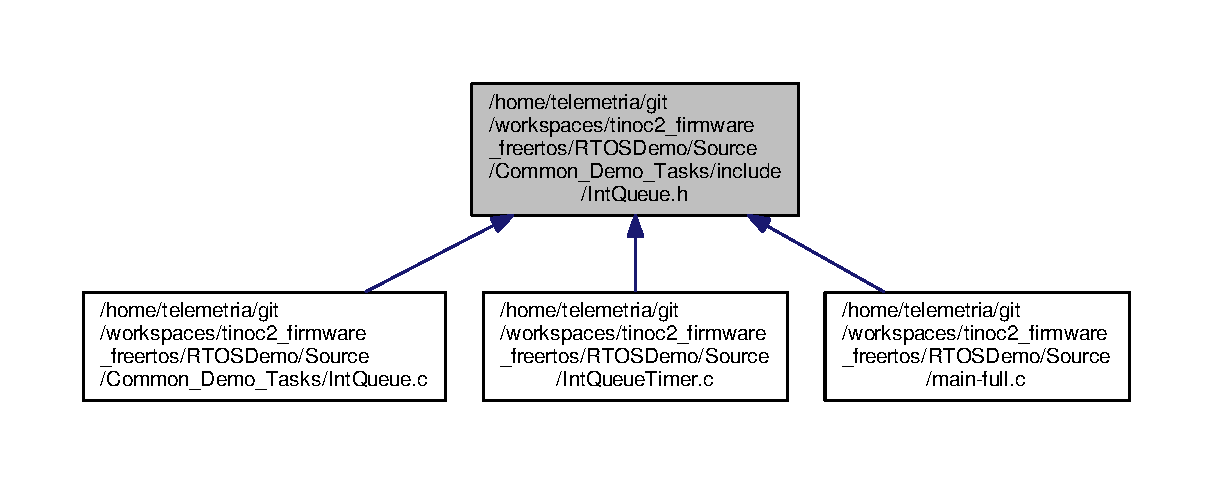
\includegraphics[width=350pt]{_int_queue_8h__dep__incl}
\end{center}
\end{figure}
\subsection*{Functions}
\begin{DoxyCompactItemize}
\item 
void \hyperlink{_int_queue_8h_a84be47a1ad79670ba1df976f3359c2f9}{v\+Start\+Interrupt\+Queue\+Tasks} (void)
\item 
\hyperlink{portmacro_8h_a46fb21e00ae0729d7515c0fbf2269796}{Base\+Type\+\_\+t} \hyperlink{_int_queue_8h_af5e2032677b21989bedf79921e3379d1}{x\+Are\+Int\+Queue\+Tasks\+Still\+Running} (void)
\item 
\hyperlink{portmacro_8h_a46fb21e00ae0729d7515c0fbf2269796}{Base\+Type\+\_\+t} \hyperlink{_int_queue_8h_a8d36998e4845da81d1a43d6c42c00527}{x\+First\+Timer\+Handler} (void)
\item 
\hyperlink{portmacro_8h_a46fb21e00ae0729d7515c0fbf2269796}{Base\+Type\+\_\+t} \hyperlink{_int_queue_8h_a3b5271af0625fcc70fa0ab05b3aa4ab7}{x\+Second\+Timer\+Handler} (void)
\end{DoxyCompactItemize}


\subsection{Function Documentation}
\index{Int\+Queue.\+h@{Int\+Queue.\+h}!v\+Start\+Interrupt\+Queue\+Tasks@{v\+Start\+Interrupt\+Queue\+Tasks}}
\index{v\+Start\+Interrupt\+Queue\+Tasks@{v\+Start\+Interrupt\+Queue\+Tasks}!Int\+Queue.\+h@{Int\+Queue.\+h}}
\subsubsection[{\texorpdfstring{v\+Start\+Interrupt\+Queue\+Tasks(void)}{vStartInterruptQueueTasks(void)}}]{\setlength{\rightskip}{0pt plus 5cm}void v\+Start\+Interrupt\+Queue\+Tasks (
\begin{DoxyParamCaption}
\item[{void}]{}
\end{DoxyParamCaption}
)}\hypertarget{_int_queue_8h_a84be47a1ad79670ba1df976f3359c2f9}{}\label{_int_queue_8h_a84be47a1ad79670ba1df976f3359c2f9}


Definition at line 239 of file Int\+Queue.\+c.

\index{Int\+Queue.\+h@{Int\+Queue.\+h}!x\+Are\+Int\+Queue\+Tasks\+Still\+Running@{x\+Are\+Int\+Queue\+Tasks\+Still\+Running}}
\index{x\+Are\+Int\+Queue\+Tasks\+Still\+Running@{x\+Are\+Int\+Queue\+Tasks\+Still\+Running}!Int\+Queue.\+h@{Int\+Queue.\+h}}
\subsubsection[{\texorpdfstring{x\+Are\+Int\+Queue\+Tasks\+Still\+Running(void)}{xAreIntQueueTasksStillRunning(void)}}]{\setlength{\rightskip}{0pt plus 5cm}{\bf Base\+Type\+\_\+t} x\+Are\+Int\+Queue\+Tasks\+Still\+Running (
\begin{DoxyParamCaption}
\item[{void}]{}
\end{DoxyParamCaption}
)}\hypertarget{_int_queue_8h_af5e2032677b21989bedf79921e3379d1}{}\label{_int_queue_8h_af5e2032677b21989bedf79921e3379d1}


Definition at line 728 of file Int\+Queue.\+c.

\index{Int\+Queue.\+h@{Int\+Queue.\+h}!x\+First\+Timer\+Handler@{x\+First\+Timer\+Handler}}
\index{x\+First\+Timer\+Handler@{x\+First\+Timer\+Handler}!Int\+Queue.\+h@{Int\+Queue.\+h}}
\subsubsection[{\texorpdfstring{x\+First\+Timer\+Handler(void)}{xFirstTimerHandler(void)}}]{\setlength{\rightskip}{0pt plus 5cm}{\bf Base\+Type\+\_\+t} x\+First\+Timer\+Handler (
\begin{DoxyParamCaption}
\item[{void}]{}
\end{DoxyParamCaption}
)}\hypertarget{_int_queue_8h_a8d36998e4845da81d1a43d6c42c00527}{}\label{_int_queue_8h_a8d36998e4845da81d1a43d6c42c00527}


Definition at line 668 of file Int\+Queue.\+c.

\index{Int\+Queue.\+h@{Int\+Queue.\+h}!x\+Second\+Timer\+Handler@{x\+Second\+Timer\+Handler}}
\index{x\+Second\+Timer\+Handler@{x\+Second\+Timer\+Handler}!Int\+Queue.\+h@{Int\+Queue.\+h}}
\subsubsection[{\texorpdfstring{x\+Second\+Timer\+Handler(void)}{xSecondTimerHandler(void)}}]{\setlength{\rightskip}{0pt plus 5cm}{\bf Base\+Type\+\_\+t} x\+Second\+Timer\+Handler (
\begin{DoxyParamCaption}
\item[{void}]{}
\end{DoxyParamCaption}
)}\hypertarget{_int_queue_8h_a3b5271af0625fcc70fa0ab05b3aa4ab7}{}\label{_int_queue_8h_a3b5271af0625fcc70fa0ab05b3aa4ab7}


Definition at line 696 of file Int\+Queue.\+c.


\hypertarget{recmutex_8h}{}\section{/home/telemetria/git/workspaces/tinoc2\+\_\+firmware\+\_\+freertos/\+R\+T\+O\+S\+Demo/\+Source/\+Common\+\_\+\+Demo\+\_\+\+Tasks/include/recmutex.h File Reference}
\label{recmutex_8h}\index{/home/telemetria/git/workspaces/tinoc2\+\_\+firmware\+\_\+freertos/\+R\+T\+O\+S\+Demo/\+Source/\+Common\+\_\+\+Demo\+\_\+\+Tasks/include/recmutex.\+h@{/home/telemetria/git/workspaces/tinoc2\+\_\+firmware\+\_\+freertos/\+R\+T\+O\+S\+Demo/\+Source/\+Common\+\_\+\+Demo\+\_\+\+Tasks/include/recmutex.\+h}}
This graph shows which files directly or indirectly include this file\+:
\nopagebreak
\begin{figure}[H]
\begin{center}
\leavevmode
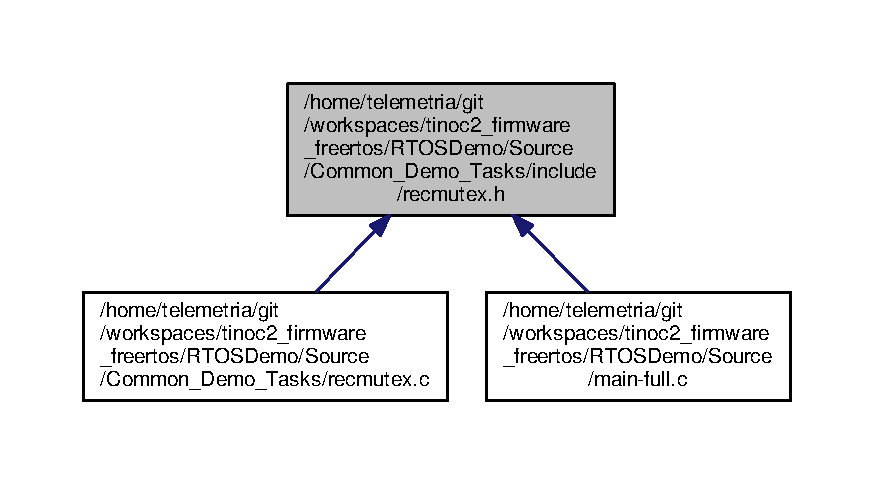
\includegraphics[width=350pt]{recmutex_8h__dep__incl}
\end{center}
\end{figure}
\subsection*{Functions}
\begin{DoxyCompactItemize}
\item 
void \hyperlink{recmutex_8h_a082ecd71608d32fd21722f1c516ab2b1}{v\+Start\+Recursive\+Mutex\+Tasks} (void)
\item 
\hyperlink{portmacro_8h_a46fb21e00ae0729d7515c0fbf2269796}{Base\+Type\+\_\+t} \hyperlink{recmutex_8h_a00c8dfcc41fab534ed6d5707e19083ab}{x\+Are\+Recursive\+Mutex\+Tasks\+Still\+Running} (void)
\end{DoxyCompactItemize}


\subsection{Function Documentation}
\index{recmutex.\+h@{recmutex.\+h}!v\+Start\+Recursive\+Mutex\+Tasks@{v\+Start\+Recursive\+Mutex\+Tasks}}
\index{v\+Start\+Recursive\+Mutex\+Tasks@{v\+Start\+Recursive\+Mutex\+Tasks}!recmutex.\+h@{recmutex.\+h}}
\subsubsection[{\texorpdfstring{v\+Start\+Recursive\+Mutex\+Tasks(void)}{vStartRecursiveMutexTasks(void)}}]{\setlength{\rightskip}{0pt plus 5cm}void v\+Start\+Recursive\+Mutex\+Tasks (
\begin{DoxyParamCaption}
\item[{void}]{}
\end{DoxyParamCaption}
)}\hypertarget{recmutex_8h_a082ecd71608d32fd21722f1c516ab2b1}{}\label{recmutex_8h_a082ecd71608d32fd21722f1c516ab2b1}


Definition at line 148 of file recmutex.\+c.

\index{recmutex.\+h@{recmutex.\+h}!x\+Are\+Recursive\+Mutex\+Tasks\+Still\+Running@{x\+Are\+Recursive\+Mutex\+Tasks\+Still\+Running}}
\index{x\+Are\+Recursive\+Mutex\+Tasks\+Still\+Running@{x\+Are\+Recursive\+Mutex\+Tasks\+Still\+Running}!recmutex.\+h@{recmutex.\+h}}
\subsubsection[{\texorpdfstring{x\+Are\+Recursive\+Mutex\+Tasks\+Still\+Running(void)}{xAreRecursiveMutexTasksStillRunning(void)}}]{\setlength{\rightskip}{0pt plus 5cm}{\bf Base\+Type\+\_\+t} x\+Are\+Recursive\+Mutex\+Tasks\+Still\+Running (
\begin{DoxyParamCaption}
\item[{void}]{}
\end{DoxyParamCaption}
)}\hypertarget{recmutex_8h_a00c8dfcc41fab534ed6d5707e19083ab}{}\label{recmutex_8h_a00c8dfcc41fab534ed6d5707e19083ab}


Definition at line 405 of file recmutex.\+c.


\hypertarget{_int_queue_8c}{}\section{/home/telemetria/git/workspaces/tinoc2\+\_\+firmware\+\_\+freertos/\+R\+T\+O\+S\+Demo/\+Source/\+Common\+\_\+\+Demo\+\_\+\+Tasks/\+Int\+Queue.c File Reference}
\label{_int_queue_8c}\index{/home/telemetria/git/workspaces/tinoc2\+\_\+firmware\+\_\+freertos/\+R\+T\+O\+S\+Demo/\+Source/\+Common\+\_\+\+Demo\+\_\+\+Tasks/\+Int\+Queue.\+c@{/home/telemetria/git/workspaces/tinoc2\+\_\+firmware\+\_\+freertos/\+R\+T\+O\+S\+Demo/\+Source/\+Common\+\_\+\+Demo\+\_\+\+Tasks/\+Int\+Queue.\+c}}
{\ttfamily \#include $<$string.\+h$>$}\\*
{\ttfamily \#include \char`\"{}Free\+R\+T\+O\+S.\+h\char`\"{}}\\*
{\ttfamily \#include \char`\"{}queue.\+h\char`\"{}}\\*
{\ttfamily \#include \char`\"{}task.\+h\char`\"{}}\\*
{\ttfamily \#include \char`\"{}Int\+Queue.\+h\char`\"{}}\\*
{\ttfamily \#include \char`\"{}Int\+Queue\+Timer.\+h\char`\"{}}\\*
Include dependency graph for Int\+Queue.\+c\+:
\nopagebreak
\begin{figure}[H]
\begin{center}
\leavevmode
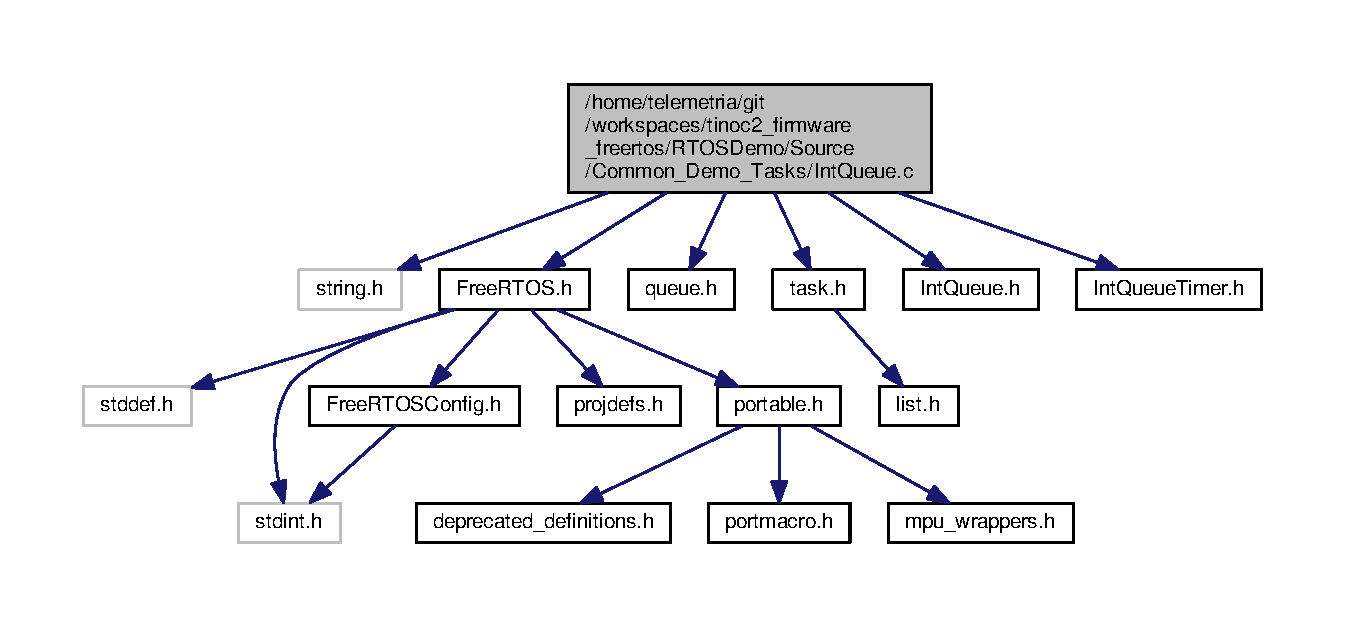
\includegraphics[width=350pt]{_int_queue_8c__incl}
\end{center}
\end{figure}
\subsection*{Macros}
\begin{DoxyCompactItemize}
\item 
\#define \hyperlink{_int_queue_8c_a6af3839a7da1a8d849039210b37f349e}{intq\+H\+I\+G\+H\+E\+R\+\_\+\+P\+R\+I\+O\+R\+I\+TY}~( \hyperlink{_free_r_t_o_s_config_8h_a9a78f5ac61e6cb172dadf2a51f11db38}{config\+M\+A\+X\+\_\+\+P\+R\+I\+O\+R\+I\+T\+I\+ES} -\/ 2 )
\item 
\#define \hyperlink{_int_queue_8c_a2627ea252ffa05b30990e49b981d3fb5}{intq\+L\+O\+W\+E\+R\+\_\+\+P\+R\+I\+O\+R\+I\+TY}~( \hyperlink{task_8h_a94ed0b9b3b4e8ccc859c322f18583e67}{tsk\+I\+D\+L\+E\+\_\+\+P\+R\+I\+O\+R\+I\+TY} )
\item 
\#define \hyperlink{_int_queue_8c_a9cc2d5d0cf4267d51442cd29da466d8c}{intq\+N\+U\+M\+\_\+\+V\+A\+L\+U\+E\+S\+\_\+\+T\+O\+\_\+\+L\+OG}~( 200 )
\item 
\#define \hyperlink{_int_queue_8c_afc04f25936cd7b39686938dc9e0706ff}{intq\+S\+H\+O\+R\+T\+\_\+\+D\+E\+L\+AY}~( 140 )
\item 
\#define \hyperlink{_int_queue_8c_a3c7ded133ee4f077b113e8f4e1911358}{intq\+V\+A\+L\+U\+E\+\_\+\+O\+V\+E\+R\+R\+UN}~( 50 )
\item 
\#define \hyperlink{_int_queue_8c_aa51a8f76a81854a21871ddc7923ceb3f}{intq\+O\+N\+E\+\_\+\+T\+I\+C\+K\+\_\+\+D\+E\+L\+AY}~( 1 )
\item 
\#define \hyperlink{_int_queue_8c_a7693bb7173910577d01e3f980dbf9ab1}{intq\+H\+I\+G\+H\+\_\+\+P\+R\+I\+O\+R\+I\+T\+Y\+\_\+\+T\+A\+S\+K1}~( ( \hyperlink{portmacro_8h_a646f89d4298e4f5afd522202b11cb2e6}{U\+Base\+Type\+\_\+t} ) 1 )
\item 
\#define \hyperlink{_int_queue_8c_a74ffd4110bd446a1cdb13cd9eee40e42}{intq\+H\+I\+G\+H\+\_\+\+P\+R\+I\+O\+R\+I\+T\+Y\+\_\+\+T\+A\+S\+K2}~( ( \hyperlink{portmacro_8h_a646f89d4298e4f5afd522202b11cb2e6}{U\+Base\+Type\+\_\+t} ) 2 )
\item 
\#define \hyperlink{_int_queue_8c_aaaf120a7be3f80b7609552a925d7804a}{intq\+L\+O\+W\+\_\+\+P\+R\+I\+O\+R\+I\+T\+Y\+\_\+\+T\+A\+SK}~( ( \hyperlink{portmacro_8h_a646f89d4298e4f5afd522202b11cb2e6}{U\+Base\+Type\+\_\+t} ) 3 )
\item 
\#define \hyperlink{_int_queue_8c_a20af9370beda829d38f4407cad1f6ce9}{intq\+F\+I\+R\+S\+T\+\_\+\+I\+N\+T\+E\+R\+R\+U\+PT}~( ( \hyperlink{portmacro_8h_a646f89d4298e4f5afd522202b11cb2e6}{U\+Base\+Type\+\_\+t} ) 4 )
\item 
\#define \hyperlink{_int_queue_8c_a77a0c87e8a0937310c6e9e529b151593}{intq\+S\+E\+C\+O\+N\+D\+\_\+\+I\+N\+T\+E\+R\+R\+U\+PT}~( ( \hyperlink{portmacro_8h_a646f89d4298e4f5afd522202b11cb2e6}{U\+Base\+Type\+\_\+t} ) 5 )
\item 
\#define \hyperlink{_int_queue_8c_adbbd09274a2525eba435ee2b03995f30}{intq\+Q\+U\+E\+U\+E\+\_\+\+L\+E\+N\+G\+TH}~( ( \hyperlink{portmacro_8h_a646f89d4298e4f5afd522202b11cb2e6}{U\+Base\+Type\+\_\+t} ) 10 )
\item 
\#define \hyperlink{_int_queue_8c_aae7b8a8d1fcc6415a731279f47a82ed7}{intq\+M\+I\+N\+\_\+\+A\+C\+C\+E\+P\+T\+A\+B\+L\+E\+\_\+\+T\+A\+S\+K\+\_\+\+C\+O\+U\+NT}~( 5 )
\item 
\#define \hyperlink{_int_queue_8c_a85236af1f0d44ac98728308a005fddcd}{timer\+N\+O\+R\+M\+A\+L\+L\+Y\+\_\+\+E\+M\+P\+T\+Y\+\_\+\+TX}()
\item 
\#define \hyperlink{_int_queue_8c_aa1f41e1ce37e0a282ac8e75a34863aac}{timer\+N\+O\+R\+M\+A\+L\+L\+Y\+\_\+\+F\+U\+L\+L\+\_\+\+TX}()
\item 
\#define \hyperlink{_int_queue_8c_aca16f9804292a4df41fac1008f5b3a8f}{timer\+N\+O\+R\+M\+A\+L\+L\+Y\+\_\+\+E\+M\+P\+T\+Y\+\_\+\+RX}()
\item 
\#define \hyperlink{_int_queue_8c_a5bde778eadfa406ac6c457019e3ab040}{timer\+N\+O\+R\+M\+A\+L\+L\+Y\+\_\+\+F\+U\+L\+L\+\_\+\+RX}()
\end{DoxyCompactItemize}
\subsection*{Functions}
\begin{DoxyCompactItemize}
\item 
static void \hyperlink{_int_queue_8c_a58d3ad6c5c87ddb30ed7d5ef8c32ee1e}{prv\+Lower\+Priority\+Normally\+Empty\+Task} (void $\ast$pv\+Parameters)
\item 
static void \hyperlink{_int_queue_8c_aa6aa65a19aa692855fd49a75722059bb}{prv\+Lower\+Priority\+Normally\+Full\+Task} (void $\ast$pv\+Parameters)
\item 
static void \hyperlink{_int_queue_8c_a1bbae63a5e2f8182b782a1f4f6a0c3d7}{prv\+Higher\+Priority\+Normally\+Empty\+Task} (void $\ast$pv\+Parameters)
\item 
static void \hyperlink{_int_queue_8c_a2a76b9ba119f55edcec9ed8208487572}{prv1st\+Higher\+Priority\+Normally\+Full\+Task} (void $\ast$pv\+Parameters)
\item 
static void \hyperlink{_int_queue_8c_aaad57f74ca166c10dfd26c45c2389d84}{prv2nd\+Higher\+Priority\+Normally\+Full\+Task} (void $\ast$pv\+Parameters)
\item 
static void \hyperlink{_int_queue_8c_a83ab696dde926ff0a5a701ed6a56005b}{prv\+Record\+Value\+\_\+\+Normally\+Empty} (\hyperlink{portmacro_8h_a646f89d4298e4f5afd522202b11cb2e6}{U\+Base\+Type\+\_\+t} ux\+Value, \hyperlink{portmacro_8h_a646f89d4298e4f5afd522202b11cb2e6}{U\+Base\+Type\+\_\+t} ux\+Source)
\item 
static void \hyperlink{_int_queue_8c_ae0708efd04b9f02c15a2bbb94264adab}{prv\+Record\+Value\+\_\+\+Normally\+Full} (\hyperlink{portmacro_8h_a646f89d4298e4f5afd522202b11cb2e6}{U\+Base\+Type\+\_\+t} ux\+Value, \hyperlink{portmacro_8h_a646f89d4298e4f5afd522202b11cb2e6}{U\+Base\+Type\+\_\+t} ux\+Source)
\item 
static void \hyperlink{_int_queue_8c_a05f375e6ea737ab45eee158ccb1a9c1d}{prv\+Queue\+Access\+Log\+Error} (\hyperlink{portmacro_8h_a646f89d4298e4f5afd522202b11cb2e6}{U\+Base\+Type\+\_\+t} ux\+Line)
\item 
void \hyperlink{_int_queue_8c_a84be47a1ad79670ba1df976f3359c2f9}{v\+Start\+Interrupt\+Queue\+Tasks} (void)
\item 
\hyperlink{portmacro_8h_a46fb21e00ae0729d7515c0fbf2269796}{Base\+Type\+\_\+t} \hyperlink{_int_queue_8c_a8d36998e4845da81d1a43d6c42c00527}{x\+First\+Timer\+Handler} (void)
\item 
\hyperlink{portmacro_8h_a46fb21e00ae0729d7515c0fbf2269796}{Base\+Type\+\_\+t} \hyperlink{_int_queue_8c_a3b5271af0625fcc70fa0ab05b3aa4ab7}{x\+Second\+Timer\+Handler} (void)
\item 
\hyperlink{portmacro_8h_a46fb21e00ae0729d7515c0fbf2269796}{Base\+Type\+\_\+t} \hyperlink{_int_queue_8c_af5e2032677b21989bedf79921e3379d1}{x\+Are\+Int\+Queue\+Tasks\+Still\+Running} (void)
\end{DoxyCompactItemize}
\subsection*{Variables}
\begin{DoxyCompactItemize}
\item 
static \hyperlink{queue_8h_aaf19d499892a4ce1409326ece00f5264}{Queue\+Handle\+\_\+t} \hyperlink{_int_queue_8c_a15676b5ef44b3cdd08f44d6a8dd1f1dc}{x\+Normally\+Empty\+Queue}
\item 
static \hyperlink{queue_8h_aaf19d499892a4ce1409326ece00f5264}{Queue\+Handle\+\_\+t} \hyperlink{_int_queue_8c_a0ebfd9346cfa0cf65759ec5026c97003}{x\+Normally\+Full\+Queue}
\item 
static volatile \hyperlink{portmacro_8h_a646f89d4298e4f5afd522202b11cb2e6}{U\+Base\+Type\+\_\+t} \hyperlink{_int_queue_8c_a3d5464d4ff74cb163bebd3ca5ce58d1a}{ux\+High\+Priority\+Loops1} = 0
\item 
static volatile \hyperlink{portmacro_8h_a646f89d4298e4f5afd522202b11cb2e6}{U\+Base\+Type\+\_\+t} \hyperlink{_int_queue_8c_aaa5d0777a5cb300bc417a185172c726f}{ux\+High\+Priority\+Loops2} = 0
\item 
static volatile \hyperlink{portmacro_8h_a646f89d4298e4f5afd522202b11cb2e6}{U\+Base\+Type\+\_\+t} \hyperlink{_int_queue_8c_af07501eaa5f89f05698aee315c476d31}{ux\+Low\+Priority\+Loops1} = 0
\item 
static volatile \hyperlink{portmacro_8h_a646f89d4298e4f5afd522202b11cb2e6}{U\+Base\+Type\+\_\+t} \hyperlink{_int_queue_8c_aac89477c692b8b0aef1fab32a27df315}{ux\+Low\+Priority\+Loops2} = 0
\item 
static \hyperlink{portmacro_8h_a46fb21e00ae0729d7515c0fbf2269796}{Base\+Type\+\_\+t} \hyperlink{_int_queue_8c_a98f15414dddf7bd58ba8362549c93ff7}{x\+Error\+Status} = \hyperlink{projdefs_8h_a07848d3078849bd32353c69d30a479b3}{pd\+P\+A\+SS}
\item 
static volatile \hyperlink{portmacro_8h_a646f89d4298e4f5afd522202b11cb2e6}{U\+Base\+Type\+\_\+t} \hyperlink{_int_queue_8c_a91d0ad6354654bc34a9a284f993c0809}{x\+Error\+Line} = ( \hyperlink{portmacro_8h_a646f89d4298e4f5afd522202b11cb2e6}{U\+Base\+Type\+\_\+t} ) 0
\item 
static \hyperlink{portmacro_8h_a46fb21e00ae0729d7515c0fbf2269796}{Base\+Type\+\_\+t} \hyperlink{_int_queue_8c_a1cce25cbf1aa2dc337322e5d328306e0}{x\+Was\+Suspended} = \hyperlink{projdefs_8h_aa56260e937e7e203026707e5ba944273}{pd\+F\+A\+L\+SE}
\item 
static volatile \hyperlink{portmacro_8h_a646f89d4298e4f5afd522202b11cb2e6}{U\+Base\+Type\+\_\+t} \hyperlink{_int_queue_8c_ab7c89b53015fe60897e0e2837542ea0a}{ux\+Value\+For\+Normally\+Empty\+Queue} = 0
\item 
static volatile \hyperlink{portmacro_8h_a646f89d4298e4f5afd522202b11cb2e6}{U\+Base\+Type\+\_\+t} \hyperlink{_int_queue_8c_ac0156b72a9329c33113e2cab0938292e}{ux\+Value\+For\+Normally\+Full\+Queue} = 0
\item 
\hyperlink{task_8h_ae95f44d4cfeb4a599c6cc258d241cb6b}{Task\+Handle\+\_\+t} \hyperlink{_int_queue_8c_abd4744cd64354335703d4b88fe475cce}{x\+High\+Priority\+Normally\+Empty\+Task1}
\item 
\hyperlink{task_8h_ae95f44d4cfeb4a599c6cc258d241cb6b}{Task\+Handle\+\_\+t} \hyperlink{_int_queue_8c_a96b7e0f1160b5ba6e9ea2b6c58cc501d}{x\+High\+Priority\+Normally\+Empty\+Task2}
\item 
\hyperlink{task_8h_ae95f44d4cfeb4a599c6cc258d241cb6b}{Task\+Handle\+\_\+t} \hyperlink{_int_queue_8c_a35639674bbc284faa76dd772811451e0}{x\+High\+Priority\+Normally\+Full\+Task1}
\item 
\hyperlink{task_8h_ae95f44d4cfeb4a599c6cc258d241cb6b}{Task\+Handle\+\_\+t} \hyperlink{_int_queue_8c_aa93f6fd7f6b23cee3afca18aa5811876}{x\+High\+Priority\+Normally\+Full\+Task2}
\item 
static uint8\+\_\+t \hyperlink{_int_queue_8c_a77e41883280e04c0c2af8c3724abc8a9}{uc\+Normally\+Empty\+Received\+Values} \mbox{[}\hyperlink{_int_queue_8c_a9cc2d5d0cf4267d51442cd29da466d8c}{intq\+N\+U\+M\+\_\+\+V\+A\+L\+U\+E\+S\+\_\+\+T\+O\+\_\+\+L\+OG}\mbox{]} = \{ 0 \}
\item 
static uint8\+\_\+t \hyperlink{_int_queue_8c_ae3074e58bb7818a07790c6f665236f09}{uc\+Normally\+Full\+Received\+Values} \mbox{[}\hyperlink{_int_queue_8c_a9cc2d5d0cf4267d51442cd29da466d8c}{intq\+N\+U\+M\+\_\+\+V\+A\+L\+U\+E\+S\+\_\+\+T\+O\+\_\+\+L\+OG}\mbox{]} = \{ 0 \}
\end{DoxyCompactItemize}


\subsection{Macro Definition Documentation}
\index{Int\+Queue.\+c@{Int\+Queue.\+c}!intq\+F\+I\+R\+S\+T\+\_\+\+I\+N\+T\+E\+R\+R\+U\+PT@{intq\+F\+I\+R\+S\+T\+\_\+\+I\+N\+T\+E\+R\+R\+U\+PT}}
\index{intq\+F\+I\+R\+S\+T\+\_\+\+I\+N\+T\+E\+R\+R\+U\+PT@{intq\+F\+I\+R\+S\+T\+\_\+\+I\+N\+T\+E\+R\+R\+U\+PT}!Int\+Queue.\+c@{Int\+Queue.\+c}}
\subsubsection[{\texorpdfstring{intq\+F\+I\+R\+S\+T\+\_\+\+I\+N\+T\+E\+R\+R\+U\+PT}{intqFIRST_INTERRUPT}}]{\setlength{\rightskip}{0pt plus 5cm}\#define intq\+F\+I\+R\+S\+T\+\_\+\+I\+N\+T\+E\+R\+R\+U\+PT~( ( {\bf U\+Base\+Type\+\_\+t} ) 4 )}\hypertarget{_int_queue_8c_a20af9370beda829d38f4407cad1f6ce9}{}\label{_int_queue_8c_a20af9370beda829d38f4407cad1f6ce9}


Definition at line 129 of file Int\+Queue.\+c.

\index{Int\+Queue.\+c@{Int\+Queue.\+c}!intq\+H\+I\+G\+H\+\_\+\+P\+R\+I\+O\+R\+I\+T\+Y\+\_\+\+T\+A\+S\+K1@{intq\+H\+I\+G\+H\+\_\+\+P\+R\+I\+O\+R\+I\+T\+Y\+\_\+\+T\+A\+S\+K1}}
\index{intq\+H\+I\+G\+H\+\_\+\+P\+R\+I\+O\+R\+I\+T\+Y\+\_\+\+T\+A\+S\+K1@{intq\+H\+I\+G\+H\+\_\+\+P\+R\+I\+O\+R\+I\+T\+Y\+\_\+\+T\+A\+S\+K1}!Int\+Queue.\+c@{Int\+Queue.\+c}}
\subsubsection[{\texorpdfstring{intq\+H\+I\+G\+H\+\_\+\+P\+R\+I\+O\+R\+I\+T\+Y\+\_\+\+T\+A\+S\+K1}{intqHIGH_PRIORITY_TASK1}}]{\setlength{\rightskip}{0pt plus 5cm}\#define intq\+H\+I\+G\+H\+\_\+\+P\+R\+I\+O\+R\+I\+T\+Y\+\_\+\+T\+A\+S\+K1~( ( {\bf U\+Base\+Type\+\_\+t} ) 1 )}\hypertarget{_int_queue_8c_a7693bb7173910577d01e3f980dbf9ab1}{}\label{_int_queue_8c_a7693bb7173910577d01e3f980dbf9ab1}


Definition at line 126 of file Int\+Queue.\+c.

\index{Int\+Queue.\+c@{Int\+Queue.\+c}!intq\+H\+I\+G\+H\+\_\+\+P\+R\+I\+O\+R\+I\+T\+Y\+\_\+\+T\+A\+S\+K2@{intq\+H\+I\+G\+H\+\_\+\+P\+R\+I\+O\+R\+I\+T\+Y\+\_\+\+T\+A\+S\+K2}}
\index{intq\+H\+I\+G\+H\+\_\+\+P\+R\+I\+O\+R\+I\+T\+Y\+\_\+\+T\+A\+S\+K2@{intq\+H\+I\+G\+H\+\_\+\+P\+R\+I\+O\+R\+I\+T\+Y\+\_\+\+T\+A\+S\+K2}!Int\+Queue.\+c@{Int\+Queue.\+c}}
\subsubsection[{\texorpdfstring{intq\+H\+I\+G\+H\+\_\+\+P\+R\+I\+O\+R\+I\+T\+Y\+\_\+\+T\+A\+S\+K2}{intqHIGH_PRIORITY_TASK2}}]{\setlength{\rightskip}{0pt plus 5cm}\#define intq\+H\+I\+G\+H\+\_\+\+P\+R\+I\+O\+R\+I\+T\+Y\+\_\+\+T\+A\+S\+K2~( ( {\bf U\+Base\+Type\+\_\+t} ) 2 )}\hypertarget{_int_queue_8c_a74ffd4110bd446a1cdb13cd9eee40e42}{}\label{_int_queue_8c_a74ffd4110bd446a1cdb13cd9eee40e42}


Definition at line 127 of file Int\+Queue.\+c.

\index{Int\+Queue.\+c@{Int\+Queue.\+c}!intq\+H\+I\+G\+H\+E\+R\+\_\+\+P\+R\+I\+O\+R\+I\+TY@{intq\+H\+I\+G\+H\+E\+R\+\_\+\+P\+R\+I\+O\+R\+I\+TY}}
\index{intq\+H\+I\+G\+H\+E\+R\+\_\+\+P\+R\+I\+O\+R\+I\+TY@{intq\+H\+I\+G\+H\+E\+R\+\_\+\+P\+R\+I\+O\+R\+I\+TY}!Int\+Queue.\+c@{Int\+Queue.\+c}}
\subsubsection[{\texorpdfstring{intq\+H\+I\+G\+H\+E\+R\+\_\+\+P\+R\+I\+O\+R\+I\+TY}{intqHIGHER_PRIORITY}}]{\setlength{\rightskip}{0pt plus 5cm}\#define intq\+H\+I\+G\+H\+E\+R\+\_\+\+P\+R\+I\+O\+R\+I\+TY~( {\bf config\+M\+A\+X\+\_\+\+P\+R\+I\+O\+R\+I\+T\+I\+ES} -\/ 2 )}\hypertarget{_int_queue_8c_a6af3839a7da1a8d849039210b37f349e}{}\label{_int_queue_8c_a6af3839a7da1a8d849039210b37f349e}


Definition at line 103 of file Int\+Queue.\+c.

\index{Int\+Queue.\+c@{Int\+Queue.\+c}!intq\+L\+O\+W\+\_\+\+P\+R\+I\+O\+R\+I\+T\+Y\+\_\+\+T\+A\+SK@{intq\+L\+O\+W\+\_\+\+P\+R\+I\+O\+R\+I\+T\+Y\+\_\+\+T\+A\+SK}}
\index{intq\+L\+O\+W\+\_\+\+P\+R\+I\+O\+R\+I\+T\+Y\+\_\+\+T\+A\+SK@{intq\+L\+O\+W\+\_\+\+P\+R\+I\+O\+R\+I\+T\+Y\+\_\+\+T\+A\+SK}!Int\+Queue.\+c@{Int\+Queue.\+c}}
\subsubsection[{\texorpdfstring{intq\+L\+O\+W\+\_\+\+P\+R\+I\+O\+R\+I\+T\+Y\+\_\+\+T\+A\+SK}{intqLOW_PRIORITY_TASK}}]{\setlength{\rightskip}{0pt plus 5cm}\#define intq\+L\+O\+W\+\_\+\+P\+R\+I\+O\+R\+I\+T\+Y\+\_\+\+T\+A\+SK~( ( {\bf U\+Base\+Type\+\_\+t} ) 3 )}\hypertarget{_int_queue_8c_aaaf120a7be3f80b7609552a925d7804a}{}\label{_int_queue_8c_aaaf120a7be3f80b7609552a925d7804a}


Definition at line 128 of file Int\+Queue.\+c.

\index{Int\+Queue.\+c@{Int\+Queue.\+c}!intq\+L\+O\+W\+E\+R\+\_\+\+P\+R\+I\+O\+R\+I\+TY@{intq\+L\+O\+W\+E\+R\+\_\+\+P\+R\+I\+O\+R\+I\+TY}}
\index{intq\+L\+O\+W\+E\+R\+\_\+\+P\+R\+I\+O\+R\+I\+TY@{intq\+L\+O\+W\+E\+R\+\_\+\+P\+R\+I\+O\+R\+I\+TY}!Int\+Queue.\+c@{Int\+Queue.\+c}}
\subsubsection[{\texorpdfstring{intq\+L\+O\+W\+E\+R\+\_\+\+P\+R\+I\+O\+R\+I\+TY}{intqLOWER_PRIORITY}}]{\setlength{\rightskip}{0pt plus 5cm}\#define intq\+L\+O\+W\+E\+R\+\_\+\+P\+R\+I\+O\+R\+I\+TY~( {\bf tsk\+I\+D\+L\+E\+\_\+\+P\+R\+I\+O\+R\+I\+TY} )}\hypertarget{_int_queue_8c_a2627ea252ffa05b30990e49b981d3fb5}{}\label{_int_queue_8c_a2627ea252ffa05b30990e49b981d3fb5}


Definition at line 105 of file Int\+Queue.\+c.

\index{Int\+Queue.\+c@{Int\+Queue.\+c}!intq\+M\+I\+N\+\_\+\+A\+C\+C\+E\+P\+T\+A\+B\+L\+E\+\_\+\+T\+A\+S\+K\+\_\+\+C\+O\+U\+NT@{intq\+M\+I\+N\+\_\+\+A\+C\+C\+E\+P\+T\+A\+B\+L\+E\+\_\+\+T\+A\+S\+K\+\_\+\+C\+O\+U\+NT}}
\index{intq\+M\+I\+N\+\_\+\+A\+C\+C\+E\+P\+T\+A\+B\+L\+E\+\_\+\+T\+A\+S\+K\+\_\+\+C\+O\+U\+NT@{intq\+M\+I\+N\+\_\+\+A\+C\+C\+E\+P\+T\+A\+B\+L\+E\+\_\+\+T\+A\+S\+K\+\_\+\+C\+O\+U\+NT}!Int\+Queue.\+c@{Int\+Queue.\+c}}
\subsubsection[{\texorpdfstring{intq\+M\+I\+N\+\_\+\+A\+C\+C\+E\+P\+T\+A\+B\+L\+E\+\_\+\+T\+A\+S\+K\+\_\+\+C\+O\+U\+NT}{intqMIN_ACCEPTABLE_TASK_COUNT}}]{\setlength{\rightskip}{0pt plus 5cm}\#define intq\+M\+I\+N\+\_\+\+A\+C\+C\+E\+P\+T\+A\+B\+L\+E\+\_\+\+T\+A\+S\+K\+\_\+\+C\+O\+U\+NT~( 5 )}\hypertarget{_int_queue_8c_aae7b8a8d1fcc6415a731279f47a82ed7}{}\label{_int_queue_8c_aae7b8a8d1fcc6415a731279f47a82ed7}


Definition at line 135 of file Int\+Queue.\+c.

\index{Int\+Queue.\+c@{Int\+Queue.\+c}!intq\+N\+U\+M\+\_\+\+V\+A\+L\+U\+E\+S\+\_\+\+T\+O\+\_\+\+L\+OG@{intq\+N\+U\+M\+\_\+\+V\+A\+L\+U\+E\+S\+\_\+\+T\+O\+\_\+\+L\+OG}}
\index{intq\+N\+U\+M\+\_\+\+V\+A\+L\+U\+E\+S\+\_\+\+T\+O\+\_\+\+L\+OG@{intq\+N\+U\+M\+\_\+\+V\+A\+L\+U\+E\+S\+\_\+\+T\+O\+\_\+\+L\+OG}!Int\+Queue.\+c@{Int\+Queue.\+c}}
\subsubsection[{\texorpdfstring{intq\+N\+U\+M\+\_\+\+V\+A\+L\+U\+E\+S\+\_\+\+T\+O\+\_\+\+L\+OG}{intqNUM_VALUES_TO_LOG}}]{\setlength{\rightskip}{0pt plus 5cm}\#define intq\+N\+U\+M\+\_\+\+V\+A\+L\+U\+E\+S\+\_\+\+T\+O\+\_\+\+L\+OG~( 200 )}\hypertarget{_int_queue_8c_a9cc2d5d0cf4267d51442cd29da466d8c}{}\label{_int_queue_8c_a9cc2d5d0cf4267d51442cd29da466d8c}


Definition at line 109 of file Int\+Queue.\+c.

\index{Int\+Queue.\+c@{Int\+Queue.\+c}!intq\+O\+N\+E\+\_\+\+T\+I\+C\+K\+\_\+\+D\+E\+L\+AY@{intq\+O\+N\+E\+\_\+\+T\+I\+C\+K\+\_\+\+D\+E\+L\+AY}}
\index{intq\+O\+N\+E\+\_\+\+T\+I\+C\+K\+\_\+\+D\+E\+L\+AY@{intq\+O\+N\+E\+\_\+\+T\+I\+C\+K\+\_\+\+D\+E\+L\+AY}!Int\+Queue.\+c@{Int\+Queue.\+c}}
\subsubsection[{\texorpdfstring{intq\+O\+N\+E\+\_\+\+T\+I\+C\+K\+\_\+\+D\+E\+L\+AY}{intqONE_TICK_DELAY}}]{\setlength{\rightskip}{0pt plus 5cm}\#define intq\+O\+N\+E\+\_\+\+T\+I\+C\+K\+\_\+\+D\+E\+L\+AY~( 1 )}\hypertarget{_int_queue_8c_aa51a8f76a81854a21871ddc7923ceb3f}{}\label{_int_queue_8c_aa51a8f76a81854a21871ddc7923ceb3f}


Definition at line 121 of file Int\+Queue.\+c.

\index{Int\+Queue.\+c@{Int\+Queue.\+c}!intq\+Q\+U\+E\+U\+E\+\_\+\+L\+E\+N\+G\+TH@{intq\+Q\+U\+E\+U\+E\+\_\+\+L\+E\+N\+G\+TH}}
\index{intq\+Q\+U\+E\+U\+E\+\_\+\+L\+E\+N\+G\+TH@{intq\+Q\+U\+E\+U\+E\+\_\+\+L\+E\+N\+G\+TH}!Int\+Queue.\+c@{Int\+Queue.\+c}}
\subsubsection[{\texorpdfstring{intq\+Q\+U\+E\+U\+E\+\_\+\+L\+E\+N\+G\+TH}{intqQUEUE_LENGTH}}]{\setlength{\rightskip}{0pt plus 5cm}\#define intq\+Q\+U\+E\+U\+E\+\_\+\+L\+E\+N\+G\+TH~( ( {\bf U\+Base\+Type\+\_\+t} ) 10 )}\hypertarget{_int_queue_8c_adbbd09274a2525eba435ee2b03995f30}{}\label{_int_queue_8c_adbbd09274a2525eba435ee2b03995f30}


Definition at line 131 of file Int\+Queue.\+c.

\index{Int\+Queue.\+c@{Int\+Queue.\+c}!intq\+S\+E\+C\+O\+N\+D\+\_\+\+I\+N\+T\+E\+R\+R\+U\+PT@{intq\+S\+E\+C\+O\+N\+D\+\_\+\+I\+N\+T\+E\+R\+R\+U\+PT}}
\index{intq\+S\+E\+C\+O\+N\+D\+\_\+\+I\+N\+T\+E\+R\+R\+U\+PT@{intq\+S\+E\+C\+O\+N\+D\+\_\+\+I\+N\+T\+E\+R\+R\+U\+PT}!Int\+Queue.\+c@{Int\+Queue.\+c}}
\subsubsection[{\texorpdfstring{intq\+S\+E\+C\+O\+N\+D\+\_\+\+I\+N\+T\+E\+R\+R\+U\+PT}{intqSECOND_INTERRUPT}}]{\setlength{\rightskip}{0pt plus 5cm}\#define intq\+S\+E\+C\+O\+N\+D\+\_\+\+I\+N\+T\+E\+R\+R\+U\+PT~( ( {\bf U\+Base\+Type\+\_\+t} ) 5 )}\hypertarget{_int_queue_8c_a77a0c87e8a0937310c6e9e529b151593}{}\label{_int_queue_8c_a77a0c87e8a0937310c6e9e529b151593}


Definition at line 130 of file Int\+Queue.\+c.

\index{Int\+Queue.\+c@{Int\+Queue.\+c}!intq\+S\+H\+O\+R\+T\+\_\+\+D\+E\+L\+AY@{intq\+S\+H\+O\+R\+T\+\_\+\+D\+E\+L\+AY}}
\index{intq\+S\+H\+O\+R\+T\+\_\+\+D\+E\+L\+AY@{intq\+S\+H\+O\+R\+T\+\_\+\+D\+E\+L\+AY}!Int\+Queue.\+c@{Int\+Queue.\+c}}
\subsubsection[{\texorpdfstring{intq\+S\+H\+O\+R\+T\+\_\+\+D\+E\+L\+AY}{intqSHORT_DELAY}}]{\setlength{\rightskip}{0pt plus 5cm}\#define intq\+S\+H\+O\+R\+T\+\_\+\+D\+E\+L\+AY~( 140 )}\hypertarget{_int_queue_8c_afc04f25936cd7b39686938dc9e0706ff}{}\label{_int_queue_8c_afc04f25936cd7b39686938dc9e0706ff}


Definition at line 110 of file Int\+Queue.\+c.

\index{Int\+Queue.\+c@{Int\+Queue.\+c}!intq\+V\+A\+L\+U\+E\+\_\+\+O\+V\+E\+R\+R\+UN@{intq\+V\+A\+L\+U\+E\+\_\+\+O\+V\+E\+R\+R\+UN}}
\index{intq\+V\+A\+L\+U\+E\+\_\+\+O\+V\+E\+R\+R\+UN@{intq\+V\+A\+L\+U\+E\+\_\+\+O\+V\+E\+R\+R\+UN}!Int\+Queue.\+c@{Int\+Queue.\+c}}
\subsubsection[{\texorpdfstring{intq\+V\+A\+L\+U\+E\+\_\+\+O\+V\+E\+R\+R\+UN}{intqVALUE_OVERRUN}}]{\setlength{\rightskip}{0pt plus 5cm}\#define intq\+V\+A\+L\+U\+E\+\_\+\+O\+V\+E\+R\+R\+UN~( 50 )}\hypertarget{_int_queue_8c_a3c7ded133ee4f077b113e8f4e1911358}{}\label{_int_queue_8c_a3c7ded133ee4f077b113e8f4e1911358}


Definition at line 117 of file Int\+Queue.\+c.

\index{Int\+Queue.\+c@{Int\+Queue.\+c}!timer\+N\+O\+R\+M\+A\+L\+L\+Y\+\_\+\+E\+M\+P\+T\+Y\+\_\+\+RX@{timer\+N\+O\+R\+M\+A\+L\+L\+Y\+\_\+\+E\+M\+P\+T\+Y\+\_\+\+RX}}
\index{timer\+N\+O\+R\+M\+A\+L\+L\+Y\+\_\+\+E\+M\+P\+T\+Y\+\_\+\+RX@{timer\+N\+O\+R\+M\+A\+L\+L\+Y\+\_\+\+E\+M\+P\+T\+Y\+\_\+\+RX}!Int\+Queue.\+c@{Int\+Queue.\+c}}
\subsubsection[{\texorpdfstring{timer\+N\+O\+R\+M\+A\+L\+L\+Y\+\_\+\+E\+M\+P\+T\+Y\+\_\+\+RX}{timerNORMALLY_EMPTY_RX}}]{\setlength{\rightskip}{0pt plus 5cm}\#define timer\+N\+O\+R\+M\+A\+L\+L\+Y\+\_\+\+E\+M\+P\+T\+Y\+\_\+\+RX(
\begin{DoxyParamCaption}
{}
\end{DoxyParamCaption}
)}\hypertarget{_int_queue_8c_aca16f9804292a4df41fac1008f5b3a8f}{}\label{_int_queue_8c_aca16f9804292a4df41fac1008f5b3a8f}
{\bfseries Value\+:}
\begin{DoxyCode}
\textcolor{keywordflow}{if}( \hyperlink{queue_8h_acdf528f5c91131ae2f31c669cfd65758}{xQueueReceiveFromISR}( \hyperlink{_int_queue_8c_a15676b5ef44b3cdd08f44d6a8dd1f1dc}{xNormallyEmptyQueue}, &uxRxedValue, &
      xHigherPriorityTaskWoken ) != \hyperlink{projdefs_8h_a07848d3078849bd32353c69d30a479b3}{pdPASS} )   \(\backslash\)
    \{                                                                                                       
      \hyperlink{_int_queue_8c_a05f375e6ea737ab45eee158ccb1a9c1d}{\(\backslash\)}
\hyperlink{_int_queue_8c_a05f375e6ea737ab45eee158ccb1a9c1d}{        prvQueueAccessLogError}( \_\_LINE\_\_ );                                                                 
      \(\backslash\)
    \}                                                                                                       
      \(\backslash\)
    else                                                                                                    
      \(\backslash\)
    \{                                                                                                       
      \hyperlink{_int_queue_8c_a83ab696dde926ff0a5a701ed6a56005b}{\(\backslash\)}
\hyperlink{_int_queue_8c_a83ab696dde926ff0a5a701ed6a56005b}{        prvRecordValue\_NormallyEmpty}( uxRxedValue, 
      \hyperlink{_int_queue_8c_a77a0c87e8a0937310c6e9e529b151593}{intqSECOND\_INTERRUPT} );                                 \(\backslash\)
    \}
\end{DoxyCode}


Definition at line 173 of file Int\+Queue.\+c.

\index{Int\+Queue.\+c@{Int\+Queue.\+c}!timer\+N\+O\+R\+M\+A\+L\+L\+Y\+\_\+\+E\+M\+P\+T\+Y\+\_\+\+TX@{timer\+N\+O\+R\+M\+A\+L\+L\+Y\+\_\+\+E\+M\+P\+T\+Y\+\_\+\+TX}}
\index{timer\+N\+O\+R\+M\+A\+L\+L\+Y\+\_\+\+E\+M\+P\+T\+Y\+\_\+\+TX@{timer\+N\+O\+R\+M\+A\+L\+L\+Y\+\_\+\+E\+M\+P\+T\+Y\+\_\+\+TX}!Int\+Queue.\+c@{Int\+Queue.\+c}}
\subsubsection[{\texorpdfstring{timer\+N\+O\+R\+M\+A\+L\+L\+Y\+\_\+\+E\+M\+P\+T\+Y\+\_\+\+TX}{timerNORMALLY_EMPTY_TX}}]{\setlength{\rightskip}{0pt plus 5cm}\#define timer\+N\+O\+R\+M\+A\+L\+L\+Y\+\_\+\+E\+M\+P\+T\+Y\+\_\+\+TX(
\begin{DoxyParamCaption}
{}
\end{DoxyParamCaption}
)}\hypertarget{_int_queue_8c_a85236af1f0d44ac98728308a005fddcd}{}\label{_int_queue_8c_a85236af1f0d44ac98728308a005fddcd}
{\bfseries Value\+:}
\begin{DoxyCode}
\textcolor{keywordflow}{if}( \hyperlink{queue_8h_a81319b3aa562733957c5a12a088516d3}{xQueueIsQueueFullFromISR}( \hyperlink{_int_queue_8c_a15676b5ef44b3cdd08f44d6a8dd1f1dc}{xNormallyEmptyQueue} ) != 
      \hyperlink{projdefs_8h_af268cf937960eb029256bd9c4d949fbe}{pdTRUE} )                                                          \(\backslash\)
    \{                                                                                                                       
      \hyperlink{portmacro_8h_a646f89d4298e4f5afd522202b11cb2e6}{\(\backslash\)}
\hyperlink{portmacro_8h_a646f89d4298e4f5afd522202b11cb2e6}{    UBaseType\_t} uxSavedInterruptStatus;                                                                                     
      \(\backslash\)
        uxSavedInterruptStatus = \hyperlink{_free_r_t_o_s_8h_a31b4260dbc1823ba80b578f86eb15a98}{portSET\_INTERRUPT\_MASK\_FROM\_ISR}();                                                          
      \(\backslash\)
        \{                                                                                                                   
      \hyperlink{_int_queue_8c_ab7c89b53015fe60897e0e2837542ea0a}{\(\backslash\)}
\hyperlink{_int_queue_8c_ab7c89b53015fe60897e0e2837542ea0a}{            uxValueForNormallyEmptyQueue}++;                                                                                  
      \(\backslash\)
            if( \hyperlink{queue_8h_a21d5919ed26c21d121df4a4debeb643c}{xQueueSendFromISR}( \hyperlink{_int_queue_8c_a15676b5ef44b3cdd08f44d6a8dd1f1dc}{xNormallyEmptyQueue}, ( \textcolor{keywordtype}{void} * ) &
      \hyperlink{_int_queue_8c_ab7c89b53015fe60897e0e2837542ea0a}{uxValueForNormallyEmptyQueue}, &xHigherPriorityTaskWoken ) != 
      \hyperlink{projdefs_8h_a07848d3078849bd32353c69d30a479b3}{pdPASS} ) \(\backslash\)
            \{                                                                                                               
      \hyperlink{_int_queue_8c_ab7c89b53015fe60897e0e2837542ea0a}{\(\backslash\)}
\hyperlink{_int_queue_8c_ab7c89b53015fe60897e0e2837542ea0a}{                uxValueForNormallyEmptyQueue}--;                                                                             
      \(\backslash\)
            \}                                                                                                               
      \(\backslash\)
        \}                                                                                                                   
      \hyperlink{_free_r_t_o_s_8h_a2661e2c5a4e4afe5bef2ebe9872e28b3}{\(\backslash\)}
\hyperlink{_free_r_t_o_s_8h_a2661e2c5a4e4afe5bef2ebe9872e28b3}{        portCLEAR\_INTERRUPT\_MASK\_FROM\_ISR}( uxSavedInterruptStatus );                                                     
      \(\backslash\)
    \}                                                                                                                       
      \(\backslash\)
\end{DoxyCode}


Definition at line 139 of file Int\+Queue.\+c.

\index{Int\+Queue.\+c@{Int\+Queue.\+c}!timer\+N\+O\+R\+M\+A\+L\+L\+Y\+\_\+\+F\+U\+L\+L\+\_\+\+RX@{timer\+N\+O\+R\+M\+A\+L\+L\+Y\+\_\+\+F\+U\+L\+L\+\_\+\+RX}}
\index{timer\+N\+O\+R\+M\+A\+L\+L\+Y\+\_\+\+F\+U\+L\+L\+\_\+\+RX@{timer\+N\+O\+R\+M\+A\+L\+L\+Y\+\_\+\+F\+U\+L\+L\+\_\+\+RX}!Int\+Queue.\+c@{Int\+Queue.\+c}}
\subsubsection[{\texorpdfstring{timer\+N\+O\+R\+M\+A\+L\+L\+Y\+\_\+\+F\+U\+L\+L\+\_\+\+RX}{timerNORMALLY_FULL_RX}}]{\setlength{\rightskip}{0pt plus 5cm}\#define timer\+N\+O\+R\+M\+A\+L\+L\+Y\+\_\+\+F\+U\+L\+L\+\_\+\+RX(
\begin{DoxyParamCaption}
{}
\end{DoxyParamCaption}
)}\hypertarget{_int_queue_8c_a5bde778eadfa406ac6c457019e3ab040}{}\label{_int_queue_8c_a5bde778eadfa406ac6c457019e3ab040}
{\bfseries Value\+:}
\begin{DoxyCode}
\textcolor{keywordflow}{if}( \hyperlink{queue_8h_acdf528f5c91131ae2f31c669cfd65758}{xQueueReceiveFromISR}( \hyperlink{_int_queue_8c_a0ebfd9346cfa0cf65759ec5026c97003}{xNormallyFullQueue}, &uxRxedValue, &
      xHigherPriorityTaskWoken ) == \hyperlink{projdefs_8h_a07848d3078849bd32353c69d30a479b3}{pdPASS} )     \(\backslash\)
    \{                                                                                                       
      \hyperlink{_int_queue_8c_ae0708efd04b9f02c15a2bbb94264adab}{\(\backslash\)}
\hyperlink{_int_queue_8c_ae0708efd04b9f02c15a2bbb94264adab}{        prvRecordValue\_NormallyFull}( uxRxedValue, 
      \hyperlink{_int_queue_8c_a77a0c87e8a0937310c6e9e529b151593}{intqSECOND\_INTERRUPT} );                                 \(\backslash\)
    \}                                                                                                       
      \(\backslash\)
\end{DoxyCode}


Definition at line 185 of file Int\+Queue.\+c.

\index{Int\+Queue.\+c@{Int\+Queue.\+c}!timer\+N\+O\+R\+M\+A\+L\+L\+Y\+\_\+\+F\+U\+L\+L\+\_\+\+TX@{timer\+N\+O\+R\+M\+A\+L\+L\+Y\+\_\+\+F\+U\+L\+L\+\_\+\+TX}}
\index{timer\+N\+O\+R\+M\+A\+L\+L\+Y\+\_\+\+F\+U\+L\+L\+\_\+\+TX@{timer\+N\+O\+R\+M\+A\+L\+L\+Y\+\_\+\+F\+U\+L\+L\+\_\+\+TX}!Int\+Queue.\+c@{Int\+Queue.\+c}}
\subsubsection[{\texorpdfstring{timer\+N\+O\+R\+M\+A\+L\+L\+Y\+\_\+\+F\+U\+L\+L\+\_\+\+TX}{timerNORMALLY_FULL_TX}}]{\setlength{\rightskip}{0pt plus 5cm}\#define timer\+N\+O\+R\+M\+A\+L\+L\+Y\+\_\+\+F\+U\+L\+L\+\_\+\+TX(
\begin{DoxyParamCaption}
{}
\end{DoxyParamCaption}
)}\hypertarget{_int_queue_8c_aa1f41e1ce37e0a282ac8e75a34863aac}{}\label{_int_queue_8c_aa1f41e1ce37e0a282ac8e75a34863aac}
{\bfseries Value\+:}
\begin{DoxyCode}
\textcolor{keywordflow}{if}( \hyperlink{queue_8h_a81319b3aa562733957c5a12a088516d3}{xQueueIsQueueFullFromISR}( \hyperlink{_int_queue_8c_a0ebfd9346cfa0cf65759ec5026c97003}{xNormallyFullQueue} ) != 
      \hyperlink{projdefs_8h_af268cf937960eb029256bd9c4d949fbe}{pdTRUE} )                                                          \(\backslash\)
    \{                                                                                                                       
      \hyperlink{portmacro_8h_a646f89d4298e4f5afd522202b11cb2e6}{\(\backslash\)}
\hyperlink{portmacro_8h_a646f89d4298e4f5afd522202b11cb2e6}{    UBaseType\_t} uxSavedInterruptStatus;                                                                                     
      \(\backslash\)
        uxSavedInterruptStatus = \hyperlink{_free_r_t_o_s_8h_a31b4260dbc1823ba80b578f86eb15a98}{portSET\_INTERRUPT\_MASK\_FROM\_ISR}();                                                          
      \(\backslash\)
        \{                                                                                                                   
      \hyperlink{_int_queue_8c_ac0156b72a9329c33113e2cab0938292e}{\(\backslash\)}
\hyperlink{_int_queue_8c_ac0156b72a9329c33113e2cab0938292e}{            uxValueForNormallyFullQueue}++;                                                                                    
      \(\backslash\)
            if( \hyperlink{queue_8h_a21d5919ed26c21d121df4a4debeb643c}{xQueueSendFromISR}( \hyperlink{_int_queue_8c_a0ebfd9346cfa0cf65759ec5026c97003}{xNormallyFullQueue}, ( \textcolor{keywordtype}{void} * ) &
      \hyperlink{_int_queue_8c_ac0156b72a9329c33113e2cab0938292e}{uxValueForNormallyFullQueue}, &xHigherPriorityTaskWoken ) != 
      \hyperlink{projdefs_8h_a07848d3078849bd32353c69d30a479b3}{pdPASS} ) \(\backslash\)
            \{                                                                                                               
      \hyperlink{_int_queue_8c_ac0156b72a9329c33113e2cab0938292e}{\(\backslash\)}
\hyperlink{_int_queue_8c_ac0156b72a9329c33113e2cab0938292e}{                uxValueForNormallyFullQueue}--;                                                                               
      \(\backslash\)
            \}                                                                                                               
      \(\backslash\)
        \}                                                                                                                   
      \hyperlink{_free_r_t_o_s_8h_a2661e2c5a4e4afe5bef2ebe9872e28b3}{\(\backslash\)}
\hyperlink{_free_r_t_o_s_8h_a2661e2c5a4e4afe5bef2ebe9872e28b3}{        portCLEAR\_INTERRUPT\_MASK\_FROM\_ISR}( uxSavedInterruptStatus );                                                     
      \(\backslash\)
    \}                                                                                                                       
      \(\backslash\)
\end{DoxyCode}


Definition at line 156 of file Int\+Queue.\+c.



\subsection{Function Documentation}
\index{Int\+Queue.\+c@{Int\+Queue.\+c}!prv1st\+Higher\+Priority\+Normally\+Full\+Task@{prv1st\+Higher\+Priority\+Normally\+Full\+Task}}
\index{prv1st\+Higher\+Priority\+Normally\+Full\+Task@{prv1st\+Higher\+Priority\+Normally\+Full\+Task}!Int\+Queue.\+c@{Int\+Queue.\+c}}
\subsubsection[{\texorpdfstring{prv1st\+Higher\+Priority\+Normally\+Full\+Task(void $\ast$pv\+Parameters)}{prv1stHigherPriorityNormallyFullTask(void *pvParameters)}}]{\setlength{\rightskip}{0pt plus 5cm}static void prv1st\+Higher\+Priority\+Normally\+Full\+Task (
\begin{DoxyParamCaption}
\item[{void $\ast$}]{pv\+Parameters}
\end{DoxyParamCaption}
)\hspace{0.3cm}{\ttfamily [static]}}\hypertarget{_int_queue_8c_a2a76b9ba119f55edcec9ed8208487572}{}\label{_int_queue_8c_a2a76b9ba119f55edcec9ed8208487572}


Definition at line 478 of file Int\+Queue.\+c.

\index{Int\+Queue.\+c@{Int\+Queue.\+c}!prv2nd\+Higher\+Priority\+Normally\+Full\+Task@{prv2nd\+Higher\+Priority\+Normally\+Full\+Task}}
\index{prv2nd\+Higher\+Priority\+Normally\+Full\+Task@{prv2nd\+Higher\+Priority\+Normally\+Full\+Task}!Int\+Queue.\+c@{Int\+Queue.\+c}}
\subsubsection[{\texorpdfstring{prv2nd\+Higher\+Priority\+Normally\+Full\+Task(void $\ast$pv\+Parameters)}{prv2ndHigherPriorityNormallyFullTask(void *pvParameters)}}]{\setlength{\rightskip}{0pt plus 5cm}static void prv2nd\+Higher\+Priority\+Normally\+Full\+Task (
\begin{DoxyParamCaption}
\item[{void $\ast$}]{pv\+Parameters}
\end{DoxyParamCaption}
)\hspace{0.3cm}{\ttfamily [static]}}\hypertarget{_int_queue_8c_aaad57f74ca166c10dfd26c45c2389d84}{}\label{_int_queue_8c_aaad57f74ca166c10dfd26c45c2389d84}


Definition at line 581 of file Int\+Queue.\+c.

\index{Int\+Queue.\+c@{Int\+Queue.\+c}!prv\+Higher\+Priority\+Normally\+Empty\+Task@{prv\+Higher\+Priority\+Normally\+Empty\+Task}}
\index{prv\+Higher\+Priority\+Normally\+Empty\+Task@{prv\+Higher\+Priority\+Normally\+Empty\+Task}!Int\+Queue.\+c@{Int\+Queue.\+c}}
\subsubsection[{\texorpdfstring{prv\+Higher\+Priority\+Normally\+Empty\+Task(void $\ast$pv\+Parameters)}{prvHigherPriorityNormallyEmptyTask(void *pvParameters)}}]{\setlength{\rightskip}{0pt plus 5cm}static void prv\+Higher\+Priority\+Normally\+Empty\+Task (
\begin{DoxyParamCaption}
\item[{void $\ast$}]{pv\+Parameters}
\end{DoxyParamCaption}
)\hspace{0.3cm}{\ttfamily [static]}}\hypertarget{_int_queue_8c_a1bbae63a5e2f8182b782a1f4f6a0c3d7}{}\label{_int_queue_8c_a1bbae63a5e2f8182b782a1f4f6a0c3d7}


Definition at line 307 of file Int\+Queue.\+c.

\index{Int\+Queue.\+c@{Int\+Queue.\+c}!prv\+Lower\+Priority\+Normally\+Empty\+Task@{prv\+Lower\+Priority\+Normally\+Empty\+Task}}
\index{prv\+Lower\+Priority\+Normally\+Empty\+Task@{prv\+Lower\+Priority\+Normally\+Empty\+Task}!Int\+Queue.\+c@{Int\+Queue.\+c}}
\subsubsection[{\texorpdfstring{prv\+Lower\+Priority\+Normally\+Empty\+Task(void $\ast$pv\+Parameters)}{prvLowerPriorityNormallyEmptyTask(void *pvParameters)}}]{\setlength{\rightskip}{0pt plus 5cm}static void prv\+Lower\+Priority\+Normally\+Empty\+Task (
\begin{DoxyParamCaption}
\item[{void $\ast$}]{pv\+Parameters}
\end{DoxyParamCaption}
)\hspace{0.3cm}{\ttfamily [static]}}\hypertarget{_int_queue_8c_a58d3ad6c5c87ddb30ed7d5ef8c32ee1e}{}\label{_int_queue_8c_a58d3ad6c5c87ddb30ed7d5ef8c32ee1e}


Definition at line 430 of file Int\+Queue.\+c.

\index{Int\+Queue.\+c@{Int\+Queue.\+c}!prv\+Lower\+Priority\+Normally\+Full\+Task@{prv\+Lower\+Priority\+Normally\+Full\+Task}}
\index{prv\+Lower\+Priority\+Normally\+Full\+Task@{prv\+Lower\+Priority\+Normally\+Full\+Task}!Int\+Queue.\+c@{Int\+Queue.\+c}}
\subsubsection[{\texorpdfstring{prv\+Lower\+Priority\+Normally\+Full\+Task(void $\ast$pv\+Parameters)}{prvLowerPriorityNormallyFullTask(void *pvParameters)}}]{\setlength{\rightskip}{0pt plus 5cm}static void prv\+Lower\+Priority\+Normally\+Full\+Task (
\begin{DoxyParamCaption}
\item[{void $\ast$}]{pv\+Parameters}
\end{DoxyParamCaption}
)\hspace{0.3cm}{\ttfamily [static]}}\hypertarget{_int_queue_8c_aa6aa65a19aa692855fd49a75722059bb}{}\label{_int_queue_8c_aa6aa65a19aa692855fd49a75722059bb}


Definition at line 627 of file Int\+Queue.\+c.

\index{Int\+Queue.\+c@{Int\+Queue.\+c}!prv\+Queue\+Access\+Log\+Error@{prv\+Queue\+Access\+Log\+Error}}
\index{prv\+Queue\+Access\+Log\+Error@{prv\+Queue\+Access\+Log\+Error}!Int\+Queue.\+c@{Int\+Queue.\+c}}
\subsubsection[{\texorpdfstring{prv\+Queue\+Access\+Log\+Error(\+U\+Base\+Type\+\_\+t ux\+Line)}{prvQueueAccessLogError(UBaseType_t uxLine)}}]{\setlength{\rightskip}{0pt plus 5cm}static void prv\+Queue\+Access\+Log\+Error (
\begin{DoxyParamCaption}
\item[{{\bf U\+Base\+Type\+\_\+t}}]{ux\+Line}
\end{DoxyParamCaption}
)\hspace{0.3cm}{\ttfamily [static]}}\hypertarget{_int_queue_8c_a05f375e6ea737ab45eee158ccb1a9c1d}{}\label{_int_queue_8c_a05f375e6ea737ab45eee158ccb1a9c1d}


Definition at line 299 of file Int\+Queue.\+c.

\index{Int\+Queue.\+c@{Int\+Queue.\+c}!prv\+Record\+Value\+\_\+\+Normally\+Empty@{prv\+Record\+Value\+\_\+\+Normally\+Empty}}
\index{prv\+Record\+Value\+\_\+\+Normally\+Empty@{prv\+Record\+Value\+\_\+\+Normally\+Empty}!Int\+Queue.\+c@{Int\+Queue.\+c}}
\subsubsection[{\texorpdfstring{prv\+Record\+Value\+\_\+\+Normally\+Empty(\+U\+Base\+Type\+\_\+t ux\+Value, U\+Base\+Type\+\_\+t ux\+Source)}{prvRecordValue_NormallyEmpty(UBaseType_t uxValue, UBaseType_t uxSource)}}]{\setlength{\rightskip}{0pt plus 5cm}static void prv\+Record\+Value\+\_\+\+Normally\+Empty (
\begin{DoxyParamCaption}
\item[{{\bf U\+Base\+Type\+\_\+t}}]{ux\+Value, }
\item[{{\bf U\+Base\+Type\+\_\+t}}]{ux\+Source}
\end{DoxyParamCaption}
)\hspace{0.3cm}{\ttfamily [static]}}\hypertarget{_int_queue_8c_a83ab696dde926ff0a5a701ed6a56005b}{}\label{_int_queue_8c_a83ab696dde926ff0a5a701ed6a56005b}


Definition at line 282 of file Int\+Queue.\+c.

\index{Int\+Queue.\+c@{Int\+Queue.\+c}!prv\+Record\+Value\+\_\+\+Normally\+Full@{prv\+Record\+Value\+\_\+\+Normally\+Full}}
\index{prv\+Record\+Value\+\_\+\+Normally\+Full@{prv\+Record\+Value\+\_\+\+Normally\+Full}!Int\+Queue.\+c@{Int\+Queue.\+c}}
\subsubsection[{\texorpdfstring{prv\+Record\+Value\+\_\+\+Normally\+Full(\+U\+Base\+Type\+\_\+t ux\+Value, U\+Base\+Type\+\_\+t ux\+Source)}{prvRecordValue_NormallyFull(UBaseType_t uxValue, UBaseType_t uxSource)}}]{\setlength{\rightskip}{0pt plus 5cm}static void prv\+Record\+Value\+\_\+\+Normally\+Full (
\begin{DoxyParamCaption}
\item[{{\bf U\+Base\+Type\+\_\+t}}]{ux\+Value, }
\item[{{\bf U\+Base\+Type\+\_\+t}}]{ux\+Source}
\end{DoxyParamCaption}
)\hspace{0.3cm}{\ttfamily [static]}}\hypertarget{_int_queue_8c_ae0708efd04b9f02c15a2bbb94264adab}{}\label{_int_queue_8c_ae0708efd04b9f02c15a2bbb94264adab}


Definition at line 265 of file Int\+Queue.\+c.

\index{Int\+Queue.\+c@{Int\+Queue.\+c}!v\+Start\+Interrupt\+Queue\+Tasks@{v\+Start\+Interrupt\+Queue\+Tasks}}
\index{v\+Start\+Interrupt\+Queue\+Tasks@{v\+Start\+Interrupt\+Queue\+Tasks}!Int\+Queue.\+c@{Int\+Queue.\+c}}
\subsubsection[{\texorpdfstring{v\+Start\+Interrupt\+Queue\+Tasks(void)}{vStartInterruptQueueTasks(void)}}]{\setlength{\rightskip}{0pt plus 5cm}void v\+Start\+Interrupt\+Queue\+Tasks (
\begin{DoxyParamCaption}
\item[{void}]{}
\end{DoxyParamCaption}
)}\hypertarget{_int_queue_8c_a84be47a1ad79670ba1df976f3359c2f9}{}\label{_int_queue_8c_a84be47a1ad79670ba1df976f3359c2f9}


Definition at line 239 of file Int\+Queue.\+c.

\index{Int\+Queue.\+c@{Int\+Queue.\+c}!x\+Are\+Int\+Queue\+Tasks\+Still\+Running@{x\+Are\+Int\+Queue\+Tasks\+Still\+Running}}
\index{x\+Are\+Int\+Queue\+Tasks\+Still\+Running@{x\+Are\+Int\+Queue\+Tasks\+Still\+Running}!Int\+Queue.\+c@{Int\+Queue.\+c}}
\subsubsection[{\texorpdfstring{x\+Are\+Int\+Queue\+Tasks\+Still\+Running(void)}{xAreIntQueueTasksStillRunning(void)}}]{\setlength{\rightskip}{0pt plus 5cm}{\bf Base\+Type\+\_\+t} x\+Are\+Int\+Queue\+Tasks\+Still\+Running (
\begin{DoxyParamCaption}
\item[{void}]{}
\end{DoxyParamCaption}
)}\hypertarget{_int_queue_8c_af5e2032677b21989bedf79921e3379d1}{}\label{_int_queue_8c_af5e2032677b21989bedf79921e3379d1}


Definition at line 728 of file Int\+Queue.\+c.

\index{Int\+Queue.\+c@{Int\+Queue.\+c}!x\+First\+Timer\+Handler@{x\+First\+Timer\+Handler}}
\index{x\+First\+Timer\+Handler@{x\+First\+Timer\+Handler}!Int\+Queue.\+c@{Int\+Queue.\+c}}
\subsubsection[{\texorpdfstring{x\+First\+Timer\+Handler(void)}{xFirstTimerHandler(void)}}]{\setlength{\rightskip}{0pt plus 5cm}{\bf Base\+Type\+\_\+t} x\+First\+Timer\+Handler (
\begin{DoxyParamCaption}
\item[{void}]{}
\end{DoxyParamCaption}
)}\hypertarget{_int_queue_8c_a8d36998e4845da81d1a43d6c42c00527}{}\label{_int_queue_8c_a8d36998e4845da81d1a43d6c42c00527}


Definition at line 668 of file Int\+Queue.\+c.

\index{Int\+Queue.\+c@{Int\+Queue.\+c}!x\+Second\+Timer\+Handler@{x\+Second\+Timer\+Handler}}
\index{x\+Second\+Timer\+Handler@{x\+Second\+Timer\+Handler}!Int\+Queue.\+c@{Int\+Queue.\+c}}
\subsubsection[{\texorpdfstring{x\+Second\+Timer\+Handler(void)}{xSecondTimerHandler(void)}}]{\setlength{\rightskip}{0pt plus 5cm}{\bf Base\+Type\+\_\+t} x\+Second\+Timer\+Handler (
\begin{DoxyParamCaption}
\item[{void}]{}
\end{DoxyParamCaption}
)}\hypertarget{_int_queue_8c_a3b5271af0625fcc70fa0ab05b3aa4ab7}{}\label{_int_queue_8c_a3b5271af0625fcc70fa0ab05b3aa4ab7}


Definition at line 696 of file Int\+Queue.\+c.



\subsection{Variable Documentation}
\index{Int\+Queue.\+c@{Int\+Queue.\+c}!uc\+Normally\+Empty\+Received\+Values@{uc\+Normally\+Empty\+Received\+Values}}
\index{uc\+Normally\+Empty\+Received\+Values@{uc\+Normally\+Empty\+Received\+Values}!Int\+Queue.\+c@{Int\+Queue.\+c}}
\subsubsection[{\texorpdfstring{uc\+Normally\+Empty\+Received\+Values}{ucNormallyEmptyReceivedValues}}]{\setlength{\rightskip}{0pt plus 5cm}uint8\+\_\+t uc\+Normally\+Empty\+Received\+Values\mbox{[}{\bf intq\+N\+U\+M\+\_\+\+V\+A\+L\+U\+E\+S\+\_\+\+T\+O\+\_\+\+L\+OG}\mbox{]} = \{ 0 \}\hspace{0.3cm}{\ttfamily [static]}}\hypertarget{_int_queue_8c_a77e41883280e04c0c2af8c3724abc8a9}{}\label{_int_queue_8c_a77e41883280e04c0c2af8c3724abc8a9}


Definition at line 219 of file Int\+Queue.\+c.

\index{Int\+Queue.\+c@{Int\+Queue.\+c}!uc\+Normally\+Full\+Received\+Values@{uc\+Normally\+Full\+Received\+Values}}
\index{uc\+Normally\+Full\+Received\+Values@{uc\+Normally\+Full\+Received\+Values}!Int\+Queue.\+c@{Int\+Queue.\+c}}
\subsubsection[{\texorpdfstring{uc\+Normally\+Full\+Received\+Values}{ucNormallyFullReceivedValues}}]{\setlength{\rightskip}{0pt plus 5cm}uint8\+\_\+t uc\+Normally\+Full\+Received\+Values\mbox{[}{\bf intq\+N\+U\+M\+\_\+\+V\+A\+L\+U\+E\+S\+\_\+\+T\+O\+\_\+\+L\+OG}\mbox{]} = \{ 0 \}\hspace{0.3cm}{\ttfamily [static]}}\hypertarget{_int_queue_8c_ae3074e58bb7818a07790c6f665236f09}{}\label{_int_queue_8c_ae3074e58bb7818a07790c6f665236f09}


Definition at line 220 of file Int\+Queue.\+c.

\index{Int\+Queue.\+c@{Int\+Queue.\+c}!ux\+High\+Priority\+Loops1@{ux\+High\+Priority\+Loops1}}
\index{ux\+High\+Priority\+Loops1@{ux\+High\+Priority\+Loops1}!Int\+Queue.\+c@{Int\+Queue.\+c}}
\subsubsection[{\texorpdfstring{ux\+High\+Priority\+Loops1}{uxHighPriorityLoops1}}]{\setlength{\rightskip}{0pt plus 5cm}volatile {\bf U\+Base\+Type\+\_\+t} ux\+High\+Priority\+Loops1 = 0\hspace{0.3cm}{\ttfamily [static]}}\hypertarget{_int_queue_8c_a3d5464d4ff74cb163bebd3ca5ce58d1a}{}\label{_int_queue_8c_a3d5464d4ff74cb163bebd3ca5ce58d1a}


Definition at line 198 of file Int\+Queue.\+c.

\index{Int\+Queue.\+c@{Int\+Queue.\+c}!ux\+High\+Priority\+Loops2@{ux\+High\+Priority\+Loops2}}
\index{ux\+High\+Priority\+Loops2@{ux\+High\+Priority\+Loops2}!Int\+Queue.\+c@{Int\+Queue.\+c}}
\subsubsection[{\texorpdfstring{ux\+High\+Priority\+Loops2}{uxHighPriorityLoops2}}]{\setlength{\rightskip}{0pt plus 5cm}volatile {\bf U\+Base\+Type\+\_\+t} ux\+High\+Priority\+Loops2 = 0\hspace{0.3cm}{\ttfamily [static]}}\hypertarget{_int_queue_8c_aaa5d0777a5cb300bc417a185172c726f}{}\label{_int_queue_8c_aaa5d0777a5cb300bc417a185172c726f}


Definition at line 198 of file Int\+Queue.\+c.

\index{Int\+Queue.\+c@{Int\+Queue.\+c}!ux\+Low\+Priority\+Loops1@{ux\+Low\+Priority\+Loops1}}
\index{ux\+Low\+Priority\+Loops1@{ux\+Low\+Priority\+Loops1}!Int\+Queue.\+c@{Int\+Queue.\+c}}
\subsubsection[{\texorpdfstring{ux\+Low\+Priority\+Loops1}{uxLowPriorityLoops1}}]{\setlength{\rightskip}{0pt plus 5cm}volatile {\bf U\+Base\+Type\+\_\+t} ux\+Low\+Priority\+Loops1 = 0\hspace{0.3cm}{\ttfamily [static]}}\hypertarget{_int_queue_8c_af07501eaa5f89f05698aee315c476d31}{}\label{_int_queue_8c_af07501eaa5f89f05698aee315c476d31}


Definition at line 198 of file Int\+Queue.\+c.

\index{Int\+Queue.\+c@{Int\+Queue.\+c}!ux\+Low\+Priority\+Loops2@{ux\+Low\+Priority\+Loops2}}
\index{ux\+Low\+Priority\+Loops2@{ux\+Low\+Priority\+Loops2}!Int\+Queue.\+c@{Int\+Queue.\+c}}
\subsubsection[{\texorpdfstring{ux\+Low\+Priority\+Loops2}{uxLowPriorityLoops2}}]{\setlength{\rightskip}{0pt plus 5cm}volatile {\bf U\+Base\+Type\+\_\+t} ux\+Low\+Priority\+Loops2 = 0\hspace{0.3cm}{\ttfamily [static]}}\hypertarget{_int_queue_8c_aac89477c692b8b0aef1fab32a27df315}{}\label{_int_queue_8c_aac89477c692b8b0aef1fab32a27df315}


Definition at line 198 of file Int\+Queue.\+c.

\index{Int\+Queue.\+c@{Int\+Queue.\+c}!ux\+Value\+For\+Normally\+Empty\+Queue@{ux\+Value\+For\+Normally\+Empty\+Queue}}
\index{ux\+Value\+For\+Normally\+Empty\+Queue@{ux\+Value\+For\+Normally\+Empty\+Queue}!Int\+Queue.\+c@{Int\+Queue.\+c}}
\subsubsection[{\texorpdfstring{ux\+Value\+For\+Normally\+Empty\+Queue}{uxValueForNormallyEmptyQueue}}]{\setlength{\rightskip}{0pt plus 5cm}volatile {\bf U\+Base\+Type\+\_\+t} ux\+Value\+For\+Normally\+Empty\+Queue = 0\hspace{0.3cm}{\ttfamily [static]}}\hypertarget{_int_queue_8c_ab7c89b53015fe60897e0e2837542ea0a}{}\label{_int_queue_8c_ab7c89b53015fe60897e0e2837542ea0a}


Definition at line 210 of file Int\+Queue.\+c.

\index{Int\+Queue.\+c@{Int\+Queue.\+c}!ux\+Value\+For\+Normally\+Full\+Queue@{ux\+Value\+For\+Normally\+Full\+Queue}}
\index{ux\+Value\+For\+Normally\+Full\+Queue@{ux\+Value\+For\+Normally\+Full\+Queue}!Int\+Queue.\+c@{Int\+Queue.\+c}}
\subsubsection[{\texorpdfstring{ux\+Value\+For\+Normally\+Full\+Queue}{uxValueForNormallyFullQueue}}]{\setlength{\rightskip}{0pt plus 5cm}volatile {\bf U\+Base\+Type\+\_\+t} ux\+Value\+For\+Normally\+Full\+Queue = 0\hspace{0.3cm}{\ttfamily [static]}}\hypertarget{_int_queue_8c_ac0156b72a9329c33113e2cab0938292e}{}\label{_int_queue_8c_ac0156b72a9329c33113e2cab0938292e}


Definition at line 210 of file Int\+Queue.\+c.

\index{Int\+Queue.\+c@{Int\+Queue.\+c}!x\+Error\+Line@{x\+Error\+Line}}
\index{x\+Error\+Line@{x\+Error\+Line}!Int\+Queue.\+c@{Int\+Queue.\+c}}
\subsubsection[{\texorpdfstring{x\+Error\+Line}{xErrorLine}}]{\setlength{\rightskip}{0pt plus 5cm}volatile {\bf U\+Base\+Type\+\_\+t} x\+Error\+Line = ( {\bf U\+Base\+Type\+\_\+t} ) 0\hspace{0.3cm}{\ttfamily [static]}}\hypertarget{_int_queue_8c_a91d0ad6354654bc34a9a284f993c0809}{}\label{_int_queue_8c_a91d0ad6354654bc34a9a284f993c0809}


Definition at line 203 of file Int\+Queue.\+c.

\index{Int\+Queue.\+c@{Int\+Queue.\+c}!x\+Error\+Status@{x\+Error\+Status}}
\index{x\+Error\+Status@{x\+Error\+Status}!Int\+Queue.\+c@{Int\+Queue.\+c}}
\subsubsection[{\texorpdfstring{x\+Error\+Status}{xErrorStatus}}]{\setlength{\rightskip}{0pt plus 5cm}{\bf Base\+Type\+\_\+t} x\+Error\+Status = {\bf pd\+P\+A\+SS}\hspace{0.3cm}{\ttfamily [static]}}\hypertarget{_int_queue_8c_a98f15414dddf7bd58ba8362549c93ff7}{}\label{_int_queue_8c_a98f15414dddf7bd58ba8362549c93ff7}


Definition at line 202 of file Int\+Queue.\+c.

\index{Int\+Queue.\+c@{Int\+Queue.\+c}!x\+High\+Priority\+Normally\+Empty\+Task1@{x\+High\+Priority\+Normally\+Empty\+Task1}}
\index{x\+High\+Priority\+Normally\+Empty\+Task1@{x\+High\+Priority\+Normally\+Empty\+Task1}!Int\+Queue.\+c@{Int\+Queue.\+c}}
\subsubsection[{\texorpdfstring{x\+High\+Priority\+Normally\+Empty\+Task1}{xHighPriorityNormallyEmptyTask1}}]{\setlength{\rightskip}{0pt plus 5cm}{\bf Task\+Handle\+\_\+t} x\+High\+Priority\+Normally\+Empty\+Task1}\hypertarget{_int_queue_8c_abd4744cd64354335703d4b88fe475cce}{}\label{_int_queue_8c_abd4744cd64354335703d4b88fe475cce}


Definition at line 213 of file Int\+Queue.\+c.

\index{Int\+Queue.\+c@{Int\+Queue.\+c}!x\+High\+Priority\+Normally\+Empty\+Task2@{x\+High\+Priority\+Normally\+Empty\+Task2}}
\index{x\+High\+Priority\+Normally\+Empty\+Task2@{x\+High\+Priority\+Normally\+Empty\+Task2}!Int\+Queue.\+c@{Int\+Queue.\+c}}
\subsubsection[{\texorpdfstring{x\+High\+Priority\+Normally\+Empty\+Task2}{xHighPriorityNormallyEmptyTask2}}]{\setlength{\rightskip}{0pt plus 5cm}{\bf Task\+Handle\+\_\+t} x\+High\+Priority\+Normally\+Empty\+Task2}\hypertarget{_int_queue_8c_a96b7e0f1160b5ba6e9ea2b6c58cc501d}{}\label{_int_queue_8c_a96b7e0f1160b5ba6e9ea2b6c58cc501d}


Definition at line 213 of file Int\+Queue.\+c.

\index{Int\+Queue.\+c@{Int\+Queue.\+c}!x\+High\+Priority\+Normally\+Full\+Task1@{x\+High\+Priority\+Normally\+Full\+Task1}}
\index{x\+High\+Priority\+Normally\+Full\+Task1@{x\+High\+Priority\+Normally\+Full\+Task1}!Int\+Queue.\+c@{Int\+Queue.\+c}}
\subsubsection[{\texorpdfstring{x\+High\+Priority\+Normally\+Full\+Task1}{xHighPriorityNormallyFullTask1}}]{\setlength{\rightskip}{0pt plus 5cm}{\bf Task\+Handle\+\_\+t} x\+High\+Priority\+Normally\+Full\+Task1}\hypertarget{_int_queue_8c_a35639674bbc284faa76dd772811451e0}{}\label{_int_queue_8c_a35639674bbc284faa76dd772811451e0}


Definition at line 213 of file Int\+Queue.\+c.

\index{Int\+Queue.\+c@{Int\+Queue.\+c}!x\+High\+Priority\+Normally\+Full\+Task2@{x\+High\+Priority\+Normally\+Full\+Task2}}
\index{x\+High\+Priority\+Normally\+Full\+Task2@{x\+High\+Priority\+Normally\+Full\+Task2}!Int\+Queue.\+c@{Int\+Queue.\+c}}
\subsubsection[{\texorpdfstring{x\+High\+Priority\+Normally\+Full\+Task2}{xHighPriorityNormallyFullTask2}}]{\setlength{\rightskip}{0pt plus 5cm}{\bf Task\+Handle\+\_\+t} x\+High\+Priority\+Normally\+Full\+Task2}\hypertarget{_int_queue_8c_aa93f6fd7f6b23cee3afca18aa5811876}{}\label{_int_queue_8c_aa93f6fd7f6b23cee3afca18aa5811876}


Definition at line 213 of file Int\+Queue.\+c.

\index{Int\+Queue.\+c@{Int\+Queue.\+c}!x\+Normally\+Empty\+Queue@{x\+Normally\+Empty\+Queue}}
\index{x\+Normally\+Empty\+Queue@{x\+Normally\+Empty\+Queue}!Int\+Queue.\+c@{Int\+Queue.\+c}}
\subsubsection[{\texorpdfstring{x\+Normally\+Empty\+Queue}{xNormallyEmptyQueue}}]{\setlength{\rightskip}{0pt plus 5cm}{\bf Queue\+Handle\+\_\+t} x\+Normally\+Empty\+Queue\hspace{0.3cm}{\ttfamily [static]}}\hypertarget{_int_queue_8c_a15676b5ef44b3cdd08f44d6a8dd1f1dc}{}\label{_int_queue_8c_a15676b5ef44b3cdd08f44d6a8dd1f1dc}


Definition at line 195 of file Int\+Queue.\+c.

\index{Int\+Queue.\+c@{Int\+Queue.\+c}!x\+Normally\+Full\+Queue@{x\+Normally\+Full\+Queue}}
\index{x\+Normally\+Full\+Queue@{x\+Normally\+Full\+Queue}!Int\+Queue.\+c@{Int\+Queue.\+c}}
\subsubsection[{\texorpdfstring{x\+Normally\+Full\+Queue}{xNormallyFullQueue}}]{\setlength{\rightskip}{0pt plus 5cm}{\bf Queue\+Handle\+\_\+t} x\+Normally\+Full\+Queue\hspace{0.3cm}{\ttfamily [static]}}\hypertarget{_int_queue_8c_a0ebfd9346cfa0cf65759ec5026c97003}{}\label{_int_queue_8c_a0ebfd9346cfa0cf65759ec5026c97003}


Definition at line 195 of file Int\+Queue.\+c.

\index{Int\+Queue.\+c@{Int\+Queue.\+c}!x\+Was\+Suspended@{x\+Was\+Suspended}}
\index{x\+Was\+Suspended@{x\+Was\+Suspended}!Int\+Queue.\+c@{Int\+Queue.\+c}}
\subsubsection[{\texorpdfstring{x\+Was\+Suspended}{xWasSuspended}}]{\setlength{\rightskip}{0pt plus 5cm}{\bf Base\+Type\+\_\+t} x\+Was\+Suspended = {\bf pd\+F\+A\+L\+SE}\hspace{0.3cm}{\ttfamily [static]}}\hypertarget{_int_queue_8c_a1cce25cbf1aa2dc337322e5d328306e0}{}\label{_int_queue_8c_a1cce25cbf1aa2dc337322e5d328306e0}


Definition at line 206 of file Int\+Queue.\+c.


\hypertarget{recmutex_8c}{}\section{/home/telemetria/git/workspaces/tinoc2\+\_\+firmware\+\_\+freertos/\+R\+T\+O\+S\+Demo/\+Source/\+Common\+\_\+\+Demo\+\_\+\+Tasks/recmutex.c File Reference}
\label{recmutex_8c}\index{/home/telemetria/git/workspaces/tinoc2\+\_\+firmware\+\_\+freertos/\+R\+T\+O\+S\+Demo/\+Source/\+Common\+\_\+\+Demo\+\_\+\+Tasks/recmutex.\+c@{/home/telemetria/git/workspaces/tinoc2\+\_\+firmware\+\_\+freertos/\+R\+T\+O\+S\+Demo/\+Source/\+Common\+\_\+\+Demo\+\_\+\+Tasks/recmutex.\+c}}
{\ttfamily \#include \char`\"{}Free\+R\+T\+O\+S.\+h\char`\"{}}\\*
{\ttfamily \#include \char`\"{}task.\+h\char`\"{}}\\*
{\ttfamily \#include \char`\"{}semphr.\+h\char`\"{}}\\*
{\ttfamily \#include \char`\"{}recmutex.\+h\char`\"{}}\\*
Include dependency graph for recmutex.\+c\+:
\nopagebreak
\begin{figure}[H]
\begin{center}
\leavevmode
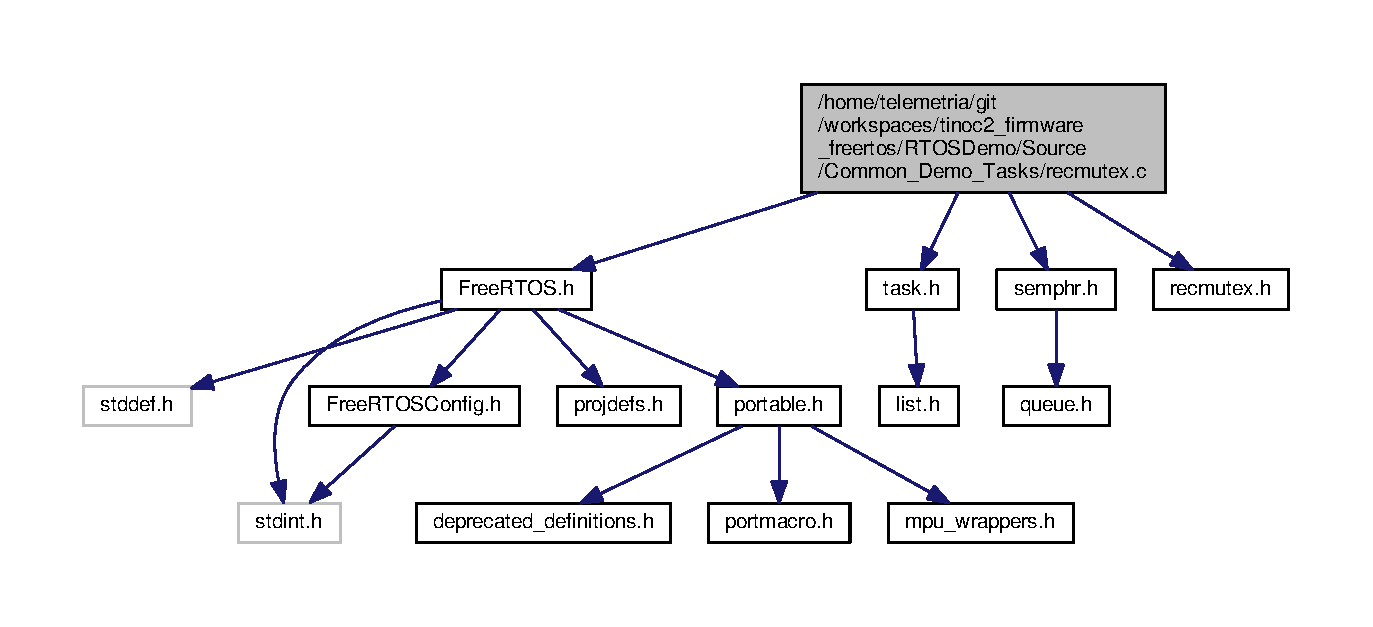
\includegraphics[width=350pt]{recmutex_8c__incl}
\end{center}
\end{figure}
\subsection*{Macros}
\begin{DoxyCompactItemize}
\item 
\#define \hyperlink{recmutex_8c_af99c9e3e4f49c0121d23c72349d56200}{recmu\+C\+O\+N\+T\+R\+O\+L\+L\+I\+N\+G\+\_\+\+T\+A\+S\+K\+\_\+\+P\+R\+I\+O\+R\+I\+TY}~( \hyperlink{task_8h_a94ed0b9b3b4e8ccc859c322f18583e67}{tsk\+I\+D\+L\+E\+\_\+\+P\+R\+I\+O\+R\+I\+TY} + 2 )
\item 
\#define \hyperlink{recmutex_8c_a5c8ccbdda8a0fc4dffd41d9c98000910}{recmu\+B\+L\+O\+C\+K\+I\+N\+G\+\_\+\+T\+A\+S\+K\+\_\+\+P\+R\+I\+O\+R\+I\+TY}~( \hyperlink{task_8h_a94ed0b9b3b4e8ccc859c322f18583e67}{tsk\+I\+D\+L\+E\+\_\+\+P\+R\+I\+O\+R\+I\+TY} + 1 )
\item 
\#define \hyperlink{recmutex_8c_ac752203198c53014c6bfc5cf121e9b80}{recmu\+P\+O\+L\+L\+I\+N\+G\+\_\+\+T\+A\+S\+K\+\_\+\+P\+R\+I\+O\+R\+I\+TY}~( \hyperlink{task_8h_a94ed0b9b3b4e8ccc859c322f18583e67}{tsk\+I\+D\+L\+E\+\_\+\+P\+R\+I\+O\+R\+I\+TY} + 0 )
\item 
\#define \hyperlink{recmutex_8c_a70a15f418f3caa45e043a6227164472c}{recmu\+M\+A\+X\+\_\+\+C\+O\+U\+NT}~( 10 )
\item 
\#define \hyperlink{recmutex_8c_ac0ec9d55855d6fc85e51e4583480e6be}{recmu\+S\+H\+O\+R\+T\+\_\+\+D\+E\+L\+AY}~( \hyperlink{projdefs_8h_a353d0f62b82a402cb3db63706c81ec3f}{pd\+M\+S\+\_\+\+T\+O\+\_\+\+T\+I\+C\+KS}( 20 ) )
\item 
\#define \hyperlink{recmutex_8c_ab8c55eaefbd120c8ca836224e4544d9c}{recmu\+N\+O\+\_\+\+D\+E\+L\+AY}~( ( \hyperlink{portmacro_8h_aa69c48c6e902ce54f70886e6573c92a9}{Tick\+Type\+\_\+t} ) 0 )
\item 
\#define \hyperlink{recmutex_8c_aec3f6c1fc5f5e04e2cf114564568374b}{recmu15ms\+\_\+\+D\+E\+L\+AY}~( \hyperlink{projdefs_8h_a353d0f62b82a402cb3db63706c81ec3f}{pd\+M\+S\+\_\+\+T\+O\+\_\+\+T\+I\+C\+KS}( 15 ) )
\end{DoxyCompactItemize}
\subsection*{Functions}
\begin{DoxyCompactItemize}
\item 
static void \hyperlink{recmutex_8c_a8d3ae703deb4830ad176c30c78c9b6f4}{prv\+Recursive\+Mutex\+Controlling\+Task} (void $\ast$pv\+Parameters)
\item 
static void \hyperlink{recmutex_8c_a515935526e4ef35eea800ae587ee53e2}{prv\+Recursive\+Mutex\+Blocking\+Task} (void $\ast$pv\+Parameters)
\item 
static void \hyperlink{recmutex_8c_a26e0ad848a0f7ae027abd41b3546192e}{prv\+Recursive\+Mutex\+Polling\+Task} (void $\ast$pv\+Parameters)
\item 
void \hyperlink{recmutex_8c_a082ecd71608d32fd21722f1c516ab2b1}{v\+Start\+Recursive\+Mutex\+Tasks} (void)
\item 
\hyperlink{portmacro_8h_a46fb21e00ae0729d7515c0fbf2269796}{Base\+Type\+\_\+t} \hyperlink{recmutex_8c_a00c8dfcc41fab534ed6d5707e19083ab}{x\+Are\+Recursive\+Mutex\+Tasks\+Still\+Running} (void)
\end{DoxyCompactItemize}
\subsection*{Variables}
\begin{DoxyCompactItemize}
\item 
static \hyperlink{semphr_8h_ad88c6df4a04beedeac782918c8a332f5}{Semaphore\+Handle\+\_\+t} \hyperlink{recmutex_8c_ae146f0f510d7944fd0e8ffd727b32f24}{x\+Mutex}
\item 
static volatile \hyperlink{portmacro_8h_a46fb21e00ae0729d7515c0fbf2269796}{Base\+Type\+\_\+t} \hyperlink{recmutex_8c_a7d608f051774754fa525a0b7481cec3a}{x\+Error\+Occurred} = \hyperlink{projdefs_8h_aa56260e937e7e203026707e5ba944273}{pd\+F\+A\+L\+SE}
\item 
static volatile \hyperlink{portmacro_8h_a46fb21e00ae0729d7515c0fbf2269796}{Base\+Type\+\_\+t} \hyperlink{recmutex_8c_af00926a8ca0127faa191f28926a87796}{x\+Controlling\+Is\+Suspended} = \hyperlink{projdefs_8h_aa56260e937e7e203026707e5ba944273}{pd\+F\+A\+L\+SE}
\item 
static volatile \hyperlink{portmacro_8h_a46fb21e00ae0729d7515c0fbf2269796}{Base\+Type\+\_\+t} \hyperlink{recmutex_8c_a92817de7a5f431666631de5c105f42b1}{x\+Blocking\+Is\+Suspended} = \hyperlink{projdefs_8h_aa56260e937e7e203026707e5ba944273}{pd\+F\+A\+L\+SE}
\item 
static volatile \hyperlink{portmacro_8h_a646f89d4298e4f5afd522202b11cb2e6}{U\+Base\+Type\+\_\+t} \hyperlink{recmutex_8c_a4451ae53a242236c983b5be292fb9c0e}{ux\+Controlling\+Cycles} = 0
\item 
static volatile \hyperlink{portmacro_8h_a646f89d4298e4f5afd522202b11cb2e6}{U\+Base\+Type\+\_\+t} \hyperlink{recmutex_8c_a884b5a24a069d68d1da5ecd50f97566c}{ux\+Blocking\+Cycles} = 0
\item 
static volatile \hyperlink{portmacro_8h_a646f89d4298e4f5afd522202b11cb2e6}{U\+Base\+Type\+\_\+t} \hyperlink{recmutex_8c_a9b14f3833255286ab7d5d66f2a8d24ce}{ux\+Polling\+Cycles} = 0
\item 
static \hyperlink{task_8h_ae95f44d4cfeb4a599c6cc258d241cb6b}{Task\+Handle\+\_\+t} \hyperlink{recmutex_8c_aaa9a1f8bd549a1a25578d170990e69fd}{x\+Controlling\+Task\+Handle}
\item 
static \hyperlink{task_8h_ae95f44d4cfeb4a599c6cc258d241cb6b}{Task\+Handle\+\_\+t} \hyperlink{recmutex_8c_aeccee32bae7c12e8a06a3ad3236032d6}{x\+Blocking\+Task\+Handle}
\end{DoxyCompactItemize}


\subsection{Macro Definition Documentation}
\index{recmutex.\+c@{recmutex.\+c}!recmu15ms\+\_\+\+D\+E\+L\+AY@{recmu15ms\+\_\+\+D\+E\+L\+AY}}
\index{recmu15ms\+\_\+\+D\+E\+L\+AY@{recmu15ms\+\_\+\+D\+E\+L\+AY}!recmutex.\+c@{recmutex.\+c}}
\subsubsection[{\texorpdfstring{recmu15ms\+\_\+\+D\+E\+L\+AY}{recmu15ms_DELAY}}]{\setlength{\rightskip}{0pt plus 5cm}\#define recmu15ms\+\_\+\+D\+E\+L\+AY~( {\bf pd\+M\+S\+\_\+\+T\+O\+\_\+\+T\+I\+C\+KS}( 15 ) )}\hypertarget{recmutex_8c_aec3f6c1fc5f5e04e2cf114564568374b}{}\label{recmutex_8c_aec3f6c1fc5f5e04e2cf114564568374b}


Definition at line 128 of file recmutex.\+c.

\index{recmutex.\+c@{recmutex.\+c}!recmu\+B\+L\+O\+C\+K\+I\+N\+G\+\_\+\+T\+A\+S\+K\+\_\+\+P\+R\+I\+O\+R\+I\+TY@{recmu\+B\+L\+O\+C\+K\+I\+N\+G\+\_\+\+T\+A\+S\+K\+\_\+\+P\+R\+I\+O\+R\+I\+TY}}
\index{recmu\+B\+L\+O\+C\+K\+I\+N\+G\+\_\+\+T\+A\+S\+K\+\_\+\+P\+R\+I\+O\+R\+I\+TY@{recmu\+B\+L\+O\+C\+K\+I\+N\+G\+\_\+\+T\+A\+S\+K\+\_\+\+P\+R\+I\+O\+R\+I\+TY}!recmutex.\+c@{recmutex.\+c}}
\subsubsection[{\texorpdfstring{recmu\+B\+L\+O\+C\+K\+I\+N\+G\+\_\+\+T\+A\+S\+K\+\_\+\+P\+R\+I\+O\+R\+I\+TY}{recmuBLOCKING_TASK_PRIORITY}}]{\setlength{\rightskip}{0pt plus 5cm}\#define recmu\+B\+L\+O\+C\+K\+I\+N\+G\+\_\+\+T\+A\+S\+K\+\_\+\+P\+R\+I\+O\+R\+I\+TY~( {\bf tsk\+I\+D\+L\+E\+\_\+\+P\+R\+I\+O\+R\+I\+TY} + 1 )}\hypertarget{recmutex_8c_a5c8ccbdda8a0fc4dffd41d9c98000910}{}\label{recmutex_8c_a5c8ccbdda8a0fc4dffd41d9c98000910}


Definition at line 119 of file recmutex.\+c.

\index{recmutex.\+c@{recmutex.\+c}!recmu\+C\+O\+N\+T\+R\+O\+L\+L\+I\+N\+G\+\_\+\+T\+A\+S\+K\+\_\+\+P\+R\+I\+O\+R\+I\+TY@{recmu\+C\+O\+N\+T\+R\+O\+L\+L\+I\+N\+G\+\_\+\+T\+A\+S\+K\+\_\+\+P\+R\+I\+O\+R\+I\+TY}}
\index{recmu\+C\+O\+N\+T\+R\+O\+L\+L\+I\+N\+G\+\_\+\+T\+A\+S\+K\+\_\+\+P\+R\+I\+O\+R\+I\+TY@{recmu\+C\+O\+N\+T\+R\+O\+L\+L\+I\+N\+G\+\_\+\+T\+A\+S\+K\+\_\+\+P\+R\+I\+O\+R\+I\+TY}!recmutex.\+c@{recmutex.\+c}}
\subsubsection[{\texorpdfstring{recmu\+C\+O\+N\+T\+R\+O\+L\+L\+I\+N\+G\+\_\+\+T\+A\+S\+K\+\_\+\+P\+R\+I\+O\+R\+I\+TY}{recmuCONTROLLING_TASK_PRIORITY}}]{\setlength{\rightskip}{0pt plus 5cm}\#define recmu\+C\+O\+N\+T\+R\+O\+L\+L\+I\+N\+G\+\_\+\+T\+A\+S\+K\+\_\+\+P\+R\+I\+O\+R\+I\+TY~( {\bf tsk\+I\+D\+L\+E\+\_\+\+P\+R\+I\+O\+R\+I\+TY} + 2 )}\hypertarget{recmutex_8c_af99c9e3e4f49c0121d23c72349d56200}{}\label{recmutex_8c_af99c9e3e4f49c0121d23c72349d56200}


Definition at line 117 of file recmutex.\+c.

\index{recmutex.\+c@{recmutex.\+c}!recmu\+M\+A\+X\+\_\+\+C\+O\+U\+NT@{recmu\+M\+A\+X\+\_\+\+C\+O\+U\+NT}}
\index{recmu\+M\+A\+X\+\_\+\+C\+O\+U\+NT@{recmu\+M\+A\+X\+\_\+\+C\+O\+U\+NT}!recmutex.\+c@{recmutex.\+c}}
\subsubsection[{\texorpdfstring{recmu\+M\+A\+X\+\_\+\+C\+O\+U\+NT}{recmuMAX_COUNT}}]{\setlength{\rightskip}{0pt plus 5cm}\#define recmu\+M\+A\+X\+\_\+\+C\+O\+U\+NT~( 10 )}\hypertarget{recmutex_8c_a70a15f418f3caa45e043a6227164472c}{}\label{recmutex_8c_a70a15f418f3caa45e043a6227164472c}


Definition at line 123 of file recmutex.\+c.

\index{recmutex.\+c@{recmutex.\+c}!recmu\+N\+O\+\_\+\+D\+E\+L\+AY@{recmu\+N\+O\+\_\+\+D\+E\+L\+AY}}
\index{recmu\+N\+O\+\_\+\+D\+E\+L\+AY@{recmu\+N\+O\+\_\+\+D\+E\+L\+AY}!recmutex.\+c@{recmutex.\+c}}
\subsubsection[{\texorpdfstring{recmu\+N\+O\+\_\+\+D\+E\+L\+AY}{recmuNO_DELAY}}]{\setlength{\rightskip}{0pt plus 5cm}\#define recmu\+N\+O\+\_\+\+D\+E\+L\+AY~( ( {\bf Tick\+Type\+\_\+t} ) 0 )}\hypertarget{recmutex_8c_ab8c55eaefbd120c8ca836224e4544d9c}{}\label{recmutex_8c_ab8c55eaefbd120c8ca836224e4544d9c}


Definition at line 127 of file recmutex.\+c.

\index{recmutex.\+c@{recmutex.\+c}!recmu\+P\+O\+L\+L\+I\+N\+G\+\_\+\+T\+A\+S\+K\+\_\+\+P\+R\+I\+O\+R\+I\+TY@{recmu\+P\+O\+L\+L\+I\+N\+G\+\_\+\+T\+A\+S\+K\+\_\+\+P\+R\+I\+O\+R\+I\+TY}}
\index{recmu\+P\+O\+L\+L\+I\+N\+G\+\_\+\+T\+A\+S\+K\+\_\+\+P\+R\+I\+O\+R\+I\+TY@{recmu\+P\+O\+L\+L\+I\+N\+G\+\_\+\+T\+A\+S\+K\+\_\+\+P\+R\+I\+O\+R\+I\+TY}!recmutex.\+c@{recmutex.\+c}}
\subsubsection[{\texorpdfstring{recmu\+P\+O\+L\+L\+I\+N\+G\+\_\+\+T\+A\+S\+K\+\_\+\+P\+R\+I\+O\+R\+I\+TY}{recmuPOLLING_TASK_PRIORITY}}]{\setlength{\rightskip}{0pt plus 5cm}\#define recmu\+P\+O\+L\+L\+I\+N\+G\+\_\+\+T\+A\+S\+K\+\_\+\+P\+R\+I\+O\+R\+I\+TY~( {\bf tsk\+I\+D\+L\+E\+\_\+\+P\+R\+I\+O\+R\+I\+TY} + 0 )}\hypertarget{recmutex_8c_ac752203198c53014c6bfc5cf121e9b80}{}\label{recmutex_8c_ac752203198c53014c6bfc5cf121e9b80}


Definition at line 120 of file recmutex.\+c.

\index{recmutex.\+c@{recmutex.\+c}!recmu\+S\+H\+O\+R\+T\+\_\+\+D\+E\+L\+AY@{recmu\+S\+H\+O\+R\+T\+\_\+\+D\+E\+L\+AY}}
\index{recmu\+S\+H\+O\+R\+T\+\_\+\+D\+E\+L\+AY@{recmu\+S\+H\+O\+R\+T\+\_\+\+D\+E\+L\+AY}!recmutex.\+c@{recmutex.\+c}}
\subsubsection[{\texorpdfstring{recmu\+S\+H\+O\+R\+T\+\_\+\+D\+E\+L\+AY}{recmuSHORT_DELAY}}]{\setlength{\rightskip}{0pt plus 5cm}\#define recmu\+S\+H\+O\+R\+T\+\_\+\+D\+E\+L\+AY~( {\bf pd\+M\+S\+\_\+\+T\+O\+\_\+\+T\+I\+C\+KS}( 20 ) )}\hypertarget{recmutex_8c_ac0ec9d55855d6fc85e51e4583480e6be}{}\label{recmutex_8c_ac0ec9d55855d6fc85e51e4583480e6be}


Definition at line 126 of file recmutex.\+c.



\subsection{Function Documentation}
\index{recmutex.\+c@{recmutex.\+c}!prv\+Recursive\+Mutex\+Blocking\+Task@{prv\+Recursive\+Mutex\+Blocking\+Task}}
\index{prv\+Recursive\+Mutex\+Blocking\+Task@{prv\+Recursive\+Mutex\+Blocking\+Task}!recmutex.\+c@{recmutex.\+c}}
\subsubsection[{\texorpdfstring{prv\+Recursive\+Mutex\+Blocking\+Task(void $\ast$pv\+Parameters)}{prvRecursiveMutexBlockingTask(void *pvParameters)}}]{\setlength{\rightskip}{0pt plus 5cm}static void prv\+Recursive\+Mutex\+Blocking\+Task (
\begin{DoxyParamCaption}
\item[{void $\ast$}]{pv\+Parameters}
\end{DoxyParamCaption}
)\hspace{0.3cm}{\ttfamily [static]}}\hypertarget{recmutex_8c_a515935526e4ef35eea800ae587ee53e2}{}\label{recmutex_8c_a515935526e4ef35eea800ae587ee53e2}


Definition at line 254 of file recmutex.\+c.

\index{recmutex.\+c@{recmutex.\+c}!prv\+Recursive\+Mutex\+Controlling\+Task@{prv\+Recursive\+Mutex\+Controlling\+Task}}
\index{prv\+Recursive\+Mutex\+Controlling\+Task@{prv\+Recursive\+Mutex\+Controlling\+Task}!recmutex.\+c@{recmutex.\+c}}
\subsubsection[{\texorpdfstring{prv\+Recursive\+Mutex\+Controlling\+Task(void $\ast$pv\+Parameters)}{prvRecursiveMutexControllingTask(void *pvParameters)}}]{\setlength{\rightskip}{0pt plus 5cm}static void prv\+Recursive\+Mutex\+Controlling\+Task (
\begin{DoxyParamCaption}
\item[{void $\ast$}]{pv\+Parameters}
\end{DoxyParamCaption}
)\hspace{0.3cm}{\ttfamily [static]}}\hypertarget{recmutex_8c_a8d3ae703deb4830ad176c30c78c9b6f4}{}\label{recmutex_8c_a8d3ae703deb4830ad176c30c78c9b6f4}


Definition at line 171 of file recmutex.\+c.

\index{recmutex.\+c@{recmutex.\+c}!prv\+Recursive\+Mutex\+Polling\+Task@{prv\+Recursive\+Mutex\+Polling\+Task}}
\index{prv\+Recursive\+Mutex\+Polling\+Task@{prv\+Recursive\+Mutex\+Polling\+Task}!recmutex.\+c@{recmutex.\+c}}
\subsubsection[{\texorpdfstring{prv\+Recursive\+Mutex\+Polling\+Task(void $\ast$pv\+Parameters)}{prvRecursiveMutexPollingTask(void *pvParameters)}}]{\setlength{\rightskip}{0pt plus 5cm}static void prv\+Recursive\+Mutex\+Polling\+Task (
\begin{DoxyParamCaption}
\item[{void $\ast$}]{pv\+Parameters}
\end{DoxyParamCaption}
)\hspace{0.3cm}{\ttfamily [static]}}\hypertarget{recmutex_8c_a26e0ad848a0f7ae027abd41b3546192e}{}\label{recmutex_8c_a26e0ad848a0f7ae027abd41b3546192e}


Definition at line 310 of file recmutex.\+c.

\index{recmutex.\+c@{recmutex.\+c}!v\+Start\+Recursive\+Mutex\+Tasks@{v\+Start\+Recursive\+Mutex\+Tasks}}
\index{v\+Start\+Recursive\+Mutex\+Tasks@{v\+Start\+Recursive\+Mutex\+Tasks}!recmutex.\+c@{recmutex.\+c}}
\subsubsection[{\texorpdfstring{v\+Start\+Recursive\+Mutex\+Tasks(void)}{vStartRecursiveMutexTasks(void)}}]{\setlength{\rightskip}{0pt plus 5cm}void v\+Start\+Recursive\+Mutex\+Tasks (
\begin{DoxyParamCaption}
\item[{void}]{}
\end{DoxyParamCaption}
)}\hypertarget{recmutex_8c_a082ecd71608d32fd21722f1c516ab2b1}{}\label{recmutex_8c_a082ecd71608d32fd21722f1c516ab2b1}


Definition at line 148 of file recmutex.\+c.

\index{recmutex.\+c@{recmutex.\+c}!x\+Are\+Recursive\+Mutex\+Tasks\+Still\+Running@{x\+Are\+Recursive\+Mutex\+Tasks\+Still\+Running}}
\index{x\+Are\+Recursive\+Mutex\+Tasks\+Still\+Running@{x\+Are\+Recursive\+Mutex\+Tasks\+Still\+Running}!recmutex.\+c@{recmutex.\+c}}
\subsubsection[{\texorpdfstring{x\+Are\+Recursive\+Mutex\+Tasks\+Still\+Running(void)}{xAreRecursiveMutexTasksStillRunning(void)}}]{\setlength{\rightskip}{0pt plus 5cm}{\bf Base\+Type\+\_\+t} x\+Are\+Recursive\+Mutex\+Tasks\+Still\+Running (
\begin{DoxyParamCaption}
\item[{void}]{}
\end{DoxyParamCaption}
)}\hypertarget{recmutex_8c_a00c8dfcc41fab534ed6d5707e19083ab}{}\label{recmutex_8c_a00c8dfcc41fab534ed6d5707e19083ab}


Definition at line 405 of file recmutex.\+c.



\subsection{Variable Documentation}
\index{recmutex.\+c@{recmutex.\+c}!ux\+Blocking\+Cycles@{ux\+Blocking\+Cycles}}
\index{ux\+Blocking\+Cycles@{ux\+Blocking\+Cycles}!recmutex.\+c@{recmutex.\+c}}
\subsubsection[{\texorpdfstring{ux\+Blocking\+Cycles}{uxBlockingCycles}}]{\setlength{\rightskip}{0pt plus 5cm}volatile {\bf U\+Base\+Type\+\_\+t} ux\+Blocking\+Cycles = 0\hspace{0.3cm}{\ttfamily [static]}}\hypertarget{recmutex_8c_a884b5a24a069d68d1da5ecd50f97566c}{}\label{recmutex_8c_a884b5a24a069d68d1da5ecd50f97566c}


Definition at line 140 of file recmutex.\+c.

\index{recmutex.\+c@{recmutex.\+c}!ux\+Controlling\+Cycles@{ux\+Controlling\+Cycles}}
\index{ux\+Controlling\+Cycles@{ux\+Controlling\+Cycles}!recmutex.\+c@{recmutex.\+c}}
\subsubsection[{\texorpdfstring{ux\+Controlling\+Cycles}{uxControllingCycles}}]{\setlength{\rightskip}{0pt plus 5cm}volatile {\bf U\+Base\+Type\+\_\+t} ux\+Controlling\+Cycles = 0\hspace{0.3cm}{\ttfamily [static]}}\hypertarget{recmutex_8c_a4451ae53a242236c983b5be292fb9c0e}{}\label{recmutex_8c_a4451ae53a242236c983b5be292fb9c0e}


Definition at line 140 of file recmutex.\+c.

\index{recmutex.\+c@{recmutex.\+c}!ux\+Polling\+Cycles@{ux\+Polling\+Cycles}}
\index{ux\+Polling\+Cycles@{ux\+Polling\+Cycles}!recmutex.\+c@{recmutex.\+c}}
\subsubsection[{\texorpdfstring{ux\+Polling\+Cycles}{uxPollingCycles}}]{\setlength{\rightskip}{0pt plus 5cm}volatile {\bf U\+Base\+Type\+\_\+t} ux\+Polling\+Cycles = 0\hspace{0.3cm}{\ttfamily [static]}}\hypertarget{recmutex_8c_a9b14f3833255286ab7d5d66f2a8d24ce}{}\label{recmutex_8c_a9b14f3833255286ab7d5d66f2a8d24ce}


Definition at line 140 of file recmutex.\+c.

\index{recmutex.\+c@{recmutex.\+c}!x\+Blocking\+Is\+Suspended@{x\+Blocking\+Is\+Suspended}}
\index{x\+Blocking\+Is\+Suspended@{x\+Blocking\+Is\+Suspended}!recmutex.\+c@{recmutex.\+c}}
\subsubsection[{\texorpdfstring{x\+Blocking\+Is\+Suspended}{xBlockingIsSuspended}}]{\setlength{\rightskip}{0pt plus 5cm}volatile {\bf Base\+Type\+\_\+t} x\+Blocking\+Is\+Suspended = {\bf pd\+F\+A\+L\+SE}\hspace{0.3cm}{\ttfamily [static]}}\hypertarget{recmutex_8c_a92817de7a5f431666631de5c105f42b1}{}\label{recmutex_8c_a92817de7a5f431666631de5c105f42b1}


Definition at line 139 of file recmutex.\+c.

\index{recmutex.\+c@{recmutex.\+c}!x\+Blocking\+Task\+Handle@{x\+Blocking\+Task\+Handle}}
\index{x\+Blocking\+Task\+Handle@{x\+Blocking\+Task\+Handle}!recmutex.\+c@{recmutex.\+c}}
\subsubsection[{\texorpdfstring{x\+Blocking\+Task\+Handle}{xBlockingTaskHandle}}]{\setlength{\rightskip}{0pt plus 5cm}{\bf Task\+Handle\+\_\+t} x\+Blocking\+Task\+Handle\hspace{0.3cm}{\ttfamily [static]}}\hypertarget{recmutex_8c_aeccee32bae7c12e8a06a3ad3236032d6}{}\label{recmutex_8c_aeccee32bae7c12e8a06a3ad3236032d6}


Definition at line 144 of file recmutex.\+c.

\index{recmutex.\+c@{recmutex.\+c}!x\+Controlling\+Is\+Suspended@{x\+Controlling\+Is\+Suspended}}
\index{x\+Controlling\+Is\+Suspended@{x\+Controlling\+Is\+Suspended}!recmutex.\+c@{recmutex.\+c}}
\subsubsection[{\texorpdfstring{x\+Controlling\+Is\+Suspended}{xControllingIsSuspended}}]{\setlength{\rightskip}{0pt plus 5cm}volatile {\bf Base\+Type\+\_\+t} x\+Controlling\+Is\+Suspended = {\bf pd\+F\+A\+L\+SE}\hspace{0.3cm}{\ttfamily [static]}}\hypertarget{recmutex_8c_af00926a8ca0127faa191f28926a87796}{}\label{recmutex_8c_af00926a8ca0127faa191f28926a87796}


Definition at line 139 of file recmutex.\+c.

\index{recmutex.\+c@{recmutex.\+c}!x\+Controlling\+Task\+Handle@{x\+Controlling\+Task\+Handle}}
\index{x\+Controlling\+Task\+Handle@{x\+Controlling\+Task\+Handle}!recmutex.\+c@{recmutex.\+c}}
\subsubsection[{\texorpdfstring{x\+Controlling\+Task\+Handle}{xControllingTaskHandle}}]{\setlength{\rightskip}{0pt plus 5cm}{\bf Task\+Handle\+\_\+t} x\+Controlling\+Task\+Handle\hspace{0.3cm}{\ttfamily [static]}}\hypertarget{recmutex_8c_aaa9a1f8bd549a1a25578d170990e69fd}{}\label{recmutex_8c_aaa9a1f8bd549a1a25578d170990e69fd}


Definition at line 144 of file recmutex.\+c.

\index{recmutex.\+c@{recmutex.\+c}!x\+Error\+Occurred@{x\+Error\+Occurred}}
\index{x\+Error\+Occurred@{x\+Error\+Occurred}!recmutex.\+c@{recmutex.\+c}}
\subsubsection[{\texorpdfstring{x\+Error\+Occurred}{xErrorOccurred}}]{\setlength{\rightskip}{0pt plus 5cm}volatile {\bf Base\+Type\+\_\+t} x\+Error\+Occurred = {\bf pd\+F\+A\+L\+SE}\hspace{0.3cm}{\ttfamily [static]}}\hypertarget{recmutex_8c_a7d608f051774754fa525a0b7481cec3a}{}\label{recmutex_8c_a7d608f051774754fa525a0b7481cec3a}


Definition at line 139 of file recmutex.\+c.

\index{recmutex.\+c@{recmutex.\+c}!x\+Mutex@{x\+Mutex}}
\index{x\+Mutex@{x\+Mutex}!recmutex.\+c@{recmutex.\+c}}
\subsubsection[{\texorpdfstring{x\+Mutex}{xMutex}}]{\setlength{\rightskip}{0pt plus 5cm}{\bf Semaphore\+Handle\+\_\+t} x\+Mutex\hspace{0.3cm}{\ttfamily [static]}}\hypertarget{recmutex_8c_ae146f0f510d7944fd0e8ffd727b32f24}{}\label{recmutex_8c_ae146f0f510d7944fd0e8ffd727b32f24}


Definition at line 136 of file recmutex.\+c.


\hypertarget{cr__startup__lpc11_8c}{}\section{/home/telemetria/git/workspaces/tinoc2\+\_\+firmware\+\_\+freertos/\+R\+T\+O\+S\+Demo/\+Source/cr\+\_\+startup\+\_\+lpc11.c File Reference}
\label{cr__startup__lpc11_8c}\index{/home/telemetria/git/workspaces/tinoc2\+\_\+firmware\+\_\+freertos/\+R\+T\+O\+S\+Demo/\+Source/cr\+\_\+startup\+\_\+lpc11.\+c@{/home/telemetria/git/workspaces/tinoc2\+\_\+firmware\+\_\+freertos/\+R\+T\+O\+S\+Demo/\+Source/cr\+\_\+startup\+\_\+lpc11.\+c}}
\subsection*{Macros}
\begin{DoxyCompactItemize}
\item 
\#define \hyperlink{cr__startup__lpc11_8c_ad1480e9557edcc543498ca259cee6c7d}{W\+E\+AK}~\hyperlink{cr__startup__lpc11_8c_adce420b900676fa0caed5a713cac82fb}{\+\_\+\+\_\+attribute\+\_\+\+\_\+} ((weak))
\item 
\#define \hyperlink{cr__startup__lpc11_8c_a0bcadbfb9fcd175b07b4d0463e54397f}{A\+L\+I\+AS}(f)~\hyperlink{cr__startup__lpc11_8c_adce420b900676fa0caed5a713cac82fb}{\+\_\+\+\_\+attribute\+\_\+\+\_\+} ((weak, alias (\#f)))
\end{DoxyCompactItemize}
\subsection*{Functions}
\begin{DoxyCompactItemize}
\item 
void \hyperlink{cr__startup__lpc11_8c_a516ff8924be921fa3a1bb7754b1f5734}{Reset\+I\+SR} (void)
\item 
\hyperlink{cr__startup__lpc11_8c_ad1480e9557edcc543498ca259cee6c7d}{W\+E\+AK} void \hyperlink{cr__startup__lpc11_8c_ae5eb40c717803d8eae9630d1f7237fd7}{N\+M\+I\+\_\+\+Handler} (void)
\item 
\hyperlink{cr__startup__lpc11_8c_ad1480e9557edcc543498ca259cee6c7d}{W\+E\+AK} void \hyperlink{cr__startup__lpc11_8c_abf5d8b089d5aceaf6a281f9bb81ac731}{Hard\+Fault\+\_\+\+Handler} (void)
\item 
\hyperlink{cr__startup__lpc11_8c_ad1480e9557edcc543498ca259cee6c7d}{W\+E\+AK} void \hyperlink{cr__startup__lpc11_8c_a577b830fb6c5b70e18748693cc057c85}{S\+V\+Call\+\_\+\+Handler} (void)
\item 
\hyperlink{cr__startup__lpc11_8c_ad1480e9557edcc543498ca259cee6c7d}{W\+E\+AK} void \hyperlink{cr__startup__lpc11_8c_a24fd4a50e601121b29d900129e4602db}{Pend\+S\+V\+\_\+\+Handler} (void)
\item 
\hyperlink{cr__startup__lpc11_8c_ad1480e9557edcc543498ca259cee6c7d}{W\+E\+AK} void \hyperlink{cr__startup__lpc11_8c_ab80f32111a0725c9f4cdfb9d6c9b7f82}{Sys\+Tick\+\_\+\+Handler} (void)
\item 
\hyperlink{cr__startup__lpc11_8c_ad1480e9557edcc543498ca259cee6c7d}{W\+E\+AK} void \hyperlink{cr__startup__lpc11_8c_abf37bc77b79673bf5babd3ac42291616}{Int\+Default\+Handler} (void)
\item 
void \hyperlink{cr__startup__lpc11_8c_a052da4fb18ef06d91b58d3c786e44fea}{C\+A\+N\+\_\+\+I\+R\+Q\+Handler} (void S\+S\+P1\+\_\+\+I\+R\+Q\+Handler() \hyperlink{cr__startup__lpc11_8c_a0bcadbfb9fcd175b07b4d0463e54397f}{A\+L\+I\+AS}(\hyperlink{cr__startup__lpc11_8c_abf37bc77b79673bf5babd3ac42291616}{Int\+Default\+Handler}) void)
\item 
\hyperlink{cr__startup__lpc11_8c_adce420b900676fa0caed5a713cac82fb}{\+\_\+\+\_\+attribute\+\_\+\+\_\+} ((section(\char`\"{}.after\+\_\+vectors\char`\"{})))
\item 
void \hyperlink{cr__startup__lpc11_8c_aa1e20137f74d718e0cfad0fa134b2543}{pop\+\_\+registers\+\_\+from\+\_\+fault\+\_\+stack} (unsigned int $\ast$hardfault\+\_\+args)
\end{DoxyCompactItemize}
\subsection*{Variables}
\begin{DoxyCompactItemize}
\item 
unsigned int \hyperlink{cr__startup__lpc11_8c_aa8f8f3229652f39c672fdb9309f96247}{\+\_\+\+\_\+data\+\_\+section\+\_\+table}
\item 
unsigned int \hyperlink{cr__startup__lpc11_8c_a09092262b7b68d7b89c9dcea506c5388}{\+\_\+\+\_\+data\+\_\+section\+\_\+table\+\_\+end}
\item 
unsigned int \hyperlink{cr__startup__lpc11_8c_a5876e5d2bb28455dd6e109ceb6a328d8}{\+\_\+\+\_\+bss\+\_\+section\+\_\+table}
\item 
unsigned int \hyperlink{cr__startup__lpc11_8c_a6365f813efb5c531f6eb7f031e28e6c1}{\+\_\+\+\_\+bss\+\_\+section\+\_\+table\+\_\+end}
\end{DoxyCompactItemize}


\subsection{Macro Definition Documentation}
\index{cr\+\_\+startup\+\_\+lpc11.\+c@{cr\+\_\+startup\+\_\+lpc11.\+c}!A\+L\+I\+AS@{A\+L\+I\+AS}}
\index{A\+L\+I\+AS@{A\+L\+I\+AS}!cr\+\_\+startup\+\_\+lpc11.\+c@{cr\+\_\+startup\+\_\+lpc11.\+c}}
\subsubsection[{\texorpdfstring{A\+L\+I\+AS}{ALIAS}}]{\setlength{\rightskip}{0pt plus 5cm}\#define A\+L\+I\+AS(
\begin{DoxyParamCaption}
\item[{}]{f}
\end{DoxyParamCaption}
)~{\bf \+\_\+\+\_\+attribute\+\_\+\+\_\+} ((weak, alias (\#f)))}\hypertarget{cr__startup__lpc11_8c_a0bcadbfb9fcd175b07b4d0463e54397f}{}\label{cr__startup__lpc11_8c_a0bcadbfb9fcd175b07b4d0463e54397f}


Definition at line 46 of file cr\+\_\+startup\+\_\+lpc11.\+c.

\index{cr\+\_\+startup\+\_\+lpc11.\+c@{cr\+\_\+startup\+\_\+lpc11.\+c}!W\+E\+AK@{W\+E\+AK}}
\index{W\+E\+AK@{W\+E\+AK}!cr\+\_\+startup\+\_\+lpc11.\+c@{cr\+\_\+startup\+\_\+lpc11.\+c}}
\subsubsection[{\texorpdfstring{W\+E\+AK}{WEAK}}]{\setlength{\rightskip}{0pt plus 5cm}\#define W\+E\+AK~{\bf \+\_\+\+\_\+attribute\+\_\+\+\_\+} ((weak))}\hypertarget{cr__startup__lpc11_8c_ad1480e9557edcc543498ca259cee6c7d}{}\label{cr__startup__lpc11_8c_ad1480e9557edcc543498ca259cee6c7d}


Definition at line 45 of file cr\+\_\+startup\+\_\+lpc11.\+c.



\subsection{Function Documentation}
\index{cr\+\_\+startup\+\_\+lpc11.\+c@{cr\+\_\+startup\+\_\+lpc11.\+c}!\+\_\+\+\_\+attribute\+\_\+\+\_\+@{\+\_\+\+\_\+attribute\+\_\+\+\_\+}}
\index{\+\_\+\+\_\+attribute\+\_\+\+\_\+@{\+\_\+\+\_\+attribute\+\_\+\+\_\+}!cr\+\_\+startup\+\_\+lpc11.\+c@{cr\+\_\+startup\+\_\+lpc11.\+c}}
\subsubsection[{\texorpdfstring{\+\_\+\+\_\+attribute\+\_\+\+\_\+((section("".\+after\+\_\+vectors"")))}{__attribute__((section(".after_vectors")))}}]{\setlength{\rightskip}{0pt plus 5cm}\+\_\+\+\_\+attribute\+\_\+\+\_\+ (
\begin{DoxyParamCaption}
\item[{(section(\char`\"{}.after\+\_\+vectors\char`\"{}))}]{}
\end{DoxyParamCaption}
)}\hypertarget{cr__startup__lpc11_8c_adce420b900676fa0caed5a713cac82fb}{}\label{cr__startup__lpc11_8c_adce420b900676fa0caed5a713cac82fb}


Definition at line 200 of file cr\+\_\+startup\+\_\+lpc11.\+c.

\index{cr\+\_\+startup\+\_\+lpc11.\+c@{cr\+\_\+startup\+\_\+lpc11.\+c}!C\+A\+N\+\_\+\+I\+R\+Q\+Handler@{C\+A\+N\+\_\+\+I\+R\+Q\+Handler}}
\index{C\+A\+N\+\_\+\+I\+R\+Q\+Handler@{C\+A\+N\+\_\+\+I\+R\+Q\+Handler}!cr\+\_\+startup\+\_\+lpc11.\+c@{cr\+\_\+startup\+\_\+lpc11.\+c}}
\subsubsection[{\texorpdfstring{C\+A\+N\+\_\+\+I\+R\+Q\+Handler(void S\+S\+P1\+\_\+\+I\+R\+Q\+Handler() A\+L\+I\+A\+S(\+Int\+Default\+Handler) void)}{CAN_IRQHandler(void SSP1_IRQHandler() ALIAS(IntDefaultHandler) void)}}]{\setlength{\rightskip}{0pt plus 5cm}void C\+A\+N\+\_\+\+I\+R\+Q\+Handler (
\begin{DoxyParamCaption}
\item[{void S\+S\+P1\+\_\+\+I\+R\+Q\+Handler () {\bf A\+L\+I\+AS}({\bf Int\+Default\+Handler})}]{void}
\end{DoxyParamCaption}
)}\hypertarget{cr__startup__lpc11_8c_a052da4fb18ef06d91b58d3c786e44fea}{}\label{cr__startup__lpc11_8c_a052da4fb18ef06d91b58d3c786e44fea}


Definition at line 82 of file cr\+\_\+startup\+\_\+lpc11.\+c.

\index{cr\+\_\+startup\+\_\+lpc11.\+c@{cr\+\_\+startup\+\_\+lpc11.\+c}!Hard\+Fault\+\_\+\+Handler@{Hard\+Fault\+\_\+\+Handler}}
\index{Hard\+Fault\+\_\+\+Handler@{Hard\+Fault\+\_\+\+Handler}!cr\+\_\+startup\+\_\+lpc11.\+c@{cr\+\_\+startup\+\_\+lpc11.\+c}}
\subsubsection[{\texorpdfstring{Hard\+Fault\+\_\+\+Handler(void)}{HardFault_Handler(void)}}]{\setlength{\rightskip}{0pt plus 5cm}{\bf W\+E\+AK} void Hard\+Fault\+\_\+\+Handler (
\begin{DoxyParamCaption}
\item[{void}]{}
\end{DoxyParamCaption}
)}\hypertarget{cr__startup__lpc11_8c_abf5d8b089d5aceaf6a281f9bb81ac731}{}\label{cr__startup__lpc11_8c_abf5d8b089d5aceaf6a281f9bb81ac731}
\index{cr\+\_\+startup\+\_\+lpc11.\+c@{cr\+\_\+startup\+\_\+lpc11.\+c}!Int\+Default\+Handler@{Int\+Default\+Handler}}
\index{Int\+Default\+Handler@{Int\+Default\+Handler}!cr\+\_\+startup\+\_\+lpc11.\+c@{cr\+\_\+startup\+\_\+lpc11.\+c}}
\subsubsection[{\texorpdfstring{Int\+Default\+Handler(void)}{IntDefaultHandler(void)}}]{\setlength{\rightskip}{0pt plus 5cm}{\bf W\+E\+AK} void Int\+Default\+Handler (
\begin{DoxyParamCaption}
\item[{void}]{}
\end{DoxyParamCaption}
)}\hypertarget{cr__startup__lpc11_8c_abf37bc77b79673bf5babd3ac42291616}{}\label{cr__startup__lpc11_8c_abf37bc77b79673bf5babd3ac42291616}
\index{cr\+\_\+startup\+\_\+lpc11.\+c@{cr\+\_\+startup\+\_\+lpc11.\+c}!N\+M\+I\+\_\+\+Handler@{N\+M\+I\+\_\+\+Handler}}
\index{N\+M\+I\+\_\+\+Handler@{N\+M\+I\+\_\+\+Handler}!cr\+\_\+startup\+\_\+lpc11.\+c@{cr\+\_\+startup\+\_\+lpc11.\+c}}
\subsubsection[{\texorpdfstring{N\+M\+I\+\_\+\+Handler(void)}{NMI_Handler(void)}}]{\setlength{\rightskip}{0pt plus 5cm}{\bf W\+E\+AK} void N\+M\+I\+\_\+\+Handler (
\begin{DoxyParamCaption}
\item[{void}]{}
\end{DoxyParamCaption}
)}\hypertarget{cr__startup__lpc11_8c_ae5eb40c717803d8eae9630d1f7237fd7}{}\label{cr__startup__lpc11_8c_ae5eb40c717803d8eae9630d1f7237fd7}
\index{cr\+\_\+startup\+\_\+lpc11.\+c@{cr\+\_\+startup\+\_\+lpc11.\+c}!Pend\+S\+V\+\_\+\+Handler@{Pend\+S\+V\+\_\+\+Handler}}
\index{Pend\+S\+V\+\_\+\+Handler@{Pend\+S\+V\+\_\+\+Handler}!cr\+\_\+startup\+\_\+lpc11.\+c@{cr\+\_\+startup\+\_\+lpc11.\+c}}
\subsubsection[{\texorpdfstring{Pend\+S\+V\+\_\+\+Handler(void)}{PendSV_Handler(void)}}]{\setlength{\rightskip}{0pt plus 5cm}{\bf W\+E\+AK} void Pend\+S\+V\+\_\+\+Handler (
\begin{DoxyParamCaption}
\item[{void}]{}
\end{DoxyParamCaption}
)}\hypertarget{cr__startup__lpc11_8c_a24fd4a50e601121b29d900129e4602db}{}\label{cr__startup__lpc11_8c_a24fd4a50e601121b29d900129e4602db}
\index{cr\+\_\+startup\+\_\+lpc11.\+c@{cr\+\_\+startup\+\_\+lpc11.\+c}!pop\+\_\+registers\+\_\+from\+\_\+fault\+\_\+stack@{pop\+\_\+registers\+\_\+from\+\_\+fault\+\_\+stack}}
\index{pop\+\_\+registers\+\_\+from\+\_\+fault\+\_\+stack@{pop\+\_\+registers\+\_\+from\+\_\+fault\+\_\+stack}!cr\+\_\+startup\+\_\+lpc11.\+c@{cr\+\_\+startup\+\_\+lpc11.\+c}}
\subsubsection[{\texorpdfstring{pop\+\_\+registers\+\_\+from\+\_\+fault\+\_\+stack(unsigned int $\ast$hardfault\+\_\+args)}{pop_registers_from_fault_stack(unsigned int *hardfault_args)}}]{\setlength{\rightskip}{0pt plus 5cm}void pop\+\_\+registers\+\_\+from\+\_\+fault\+\_\+stack (
\begin{DoxyParamCaption}
\item[{unsigned int $\ast$}]{hardfault\+\_\+args}
\end{DoxyParamCaption}
)}\hypertarget{cr__startup__lpc11_8c_aa1e20137f74d718e0cfad0fa134b2543}{}\label{cr__startup__lpc11_8c_aa1e20137f74d718e0cfad0fa134b2543}


Definition at line 339 of file cr\+\_\+startup\+\_\+lpc11.\+c.

\index{cr\+\_\+startup\+\_\+lpc11.\+c@{cr\+\_\+startup\+\_\+lpc11.\+c}!Reset\+I\+SR@{Reset\+I\+SR}}
\index{Reset\+I\+SR@{Reset\+I\+SR}!cr\+\_\+startup\+\_\+lpc11.\+c@{cr\+\_\+startup\+\_\+lpc11.\+c}}
\subsubsection[{\texorpdfstring{Reset\+I\+S\+R(void)}{ResetISR(void)}}]{\setlength{\rightskip}{0pt plus 5cm}void Reset\+I\+SR (
\begin{DoxyParamCaption}
\item[{void}]{}
\end{DoxyParamCaption}
)}\hypertarget{cr__startup__lpc11_8c_a516ff8924be921fa3a1bb7754b1f5734}{}\label{cr__startup__lpc11_8c_a516ff8924be921fa3a1bb7754b1f5734}
\index{cr\+\_\+startup\+\_\+lpc11.\+c@{cr\+\_\+startup\+\_\+lpc11.\+c}!S\+V\+Call\+\_\+\+Handler@{S\+V\+Call\+\_\+\+Handler}}
\index{S\+V\+Call\+\_\+\+Handler@{S\+V\+Call\+\_\+\+Handler}!cr\+\_\+startup\+\_\+lpc11.\+c@{cr\+\_\+startup\+\_\+lpc11.\+c}}
\subsubsection[{\texorpdfstring{S\+V\+Call\+\_\+\+Handler(void)}{SVCall_Handler(void)}}]{\setlength{\rightskip}{0pt plus 5cm}{\bf W\+E\+AK} void S\+V\+Call\+\_\+\+Handler (
\begin{DoxyParamCaption}
\item[{void}]{}
\end{DoxyParamCaption}
)}\hypertarget{cr__startup__lpc11_8c_a577b830fb6c5b70e18748693cc057c85}{}\label{cr__startup__lpc11_8c_a577b830fb6c5b70e18748693cc057c85}
\index{cr\+\_\+startup\+\_\+lpc11.\+c@{cr\+\_\+startup\+\_\+lpc11.\+c}!Sys\+Tick\+\_\+\+Handler@{Sys\+Tick\+\_\+\+Handler}}
\index{Sys\+Tick\+\_\+\+Handler@{Sys\+Tick\+\_\+\+Handler}!cr\+\_\+startup\+\_\+lpc11.\+c@{cr\+\_\+startup\+\_\+lpc11.\+c}}
\subsubsection[{\texorpdfstring{Sys\+Tick\+\_\+\+Handler(void)}{SysTick_Handler(void)}}]{\setlength{\rightskip}{0pt plus 5cm}{\bf W\+E\+AK} void Sys\+Tick\+\_\+\+Handler (
\begin{DoxyParamCaption}
\item[{void}]{}
\end{DoxyParamCaption}
)}\hypertarget{cr__startup__lpc11_8c_ab80f32111a0725c9f4cdfb9d6c9b7f82}{}\label{cr__startup__lpc11_8c_ab80f32111a0725c9f4cdfb9d6c9b7f82}


\subsection{Variable Documentation}
\index{cr\+\_\+startup\+\_\+lpc11.\+c@{cr\+\_\+startup\+\_\+lpc11.\+c}!\+\_\+\+\_\+bss\+\_\+section\+\_\+table@{\+\_\+\+\_\+bss\+\_\+section\+\_\+table}}
\index{\+\_\+\+\_\+bss\+\_\+section\+\_\+table@{\+\_\+\+\_\+bss\+\_\+section\+\_\+table}!cr\+\_\+startup\+\_\+lpc11.\+c@{cr\+\_\+startup\+\_\+lpc11.\+c}}
\subsubsection[{\texorpdfstring{\+\_\+\+\_\+bss\+\_\+section\+\_\+table}{__bss_section_table}}]{\setlength{\rightskip}{0pt plus 5cm}unsigned int \+\_\+\+\_\+bss\+\_\+section\+\_\+table}\hypertarget{cr__startup__lpc11_8c_a5876e5d2bb28455dd6e109ceb6a328d8}{}\label{cr__startup__lpc11_8c_a5876e5d2bb28455dd6e109ceb6a328d8}
\index{cr\+\_\+startup\+\_\+lpc11.\+c@{cr\+\_\+startup\+\_\+lpc11.\+c}!\+\_\+\+\_\+bss\+\_\+section\+\_\+table\+\_\+end@{\+\_\+\+\_\+bss\+\_\+section\+\_\+table\+\_\+end}}
\index{\+\_\+\+\_\+bss\+\_\+section\+\_\+table\+\_\+end@{\+\_\+\+\_\+bss\+\_\+section\+\_\+table\+\_\+end}!cr\+\_\+startup\+\_\+lpc11.\+c@{cr\+\_\+startup\+\_\+lpc11.\+c}}
\subsubsection[{\texorpdfstring{\+\_\+\+\_\+bss\+\_\+section\+\_\+table\+\_\+end}{__bss_section_table_end}}]{\setlength{\rightskip}{0pt plus 5cm}unsigned int \+\_\+\+\_\+bss\+\_\+section\+\_\+table\+\_\+end}\hypertarget{cr__startup__lpc11_8c_a6365f813efb5c531f6eb7f031e28e6c1}{}\label{cr__startup__lpc11_8c_a6365f813efb5c531f6eb7f031e28e6c1}
\index{cr\+\_\+startup\+\_\+lpc11.\+c@{cr\+\_\+startup\+\_\+lpc11.\+c}!\+\_\+\+\_\+data\+\_\+section\+\_\+table@{\+\_\+\+\_\+data\+\_\+section\+\_\+table}}
\index{\+\_\+\+\_\+data\+\_\+section\+\_\+table@{\+\_\+\+\_\+data\+\_\+section\+\_\+table}!cr\+\_\+startup\+\_\+lpc11.\+c@{cr\+\_\+startup\+\_\+lpc11.\+c}}
\subsubsection[{\texorpdfstring{\+\_\+\+\_\+data\+\_\+section\+\_\+table}{__data_section_table}}]{\setlength{\rightskip}{0pt plus 5cm}unsigned int \+\_\+\+\_\+data\+\_\+section\+\_\+table}\hypertarget{cr__startup__lpc11_8c_aa8f8f3229652f39c672fdb9309f96247}{}\label{cr__startup__lpc11_8c_aa8f8f3229652f39c672fdb9309f96247}
\index{cr\+\_\+startup\+\_\+lpc11.\+c@{cr\+\_\+startup\+\_\+lpc11.\+c}!\+\_\+\+\_\+data\+\_\+section\+\_\+table\+\_\+end@{\+\_\+\+\_\+data\+\_\+section\+\_\+table\+\_\+end}}
\index{\+\_\+\+\_\+data\+\_\+section\+\_\+table\+\_\+end@{\+\_\+\+\_\+data\+\_\+section\+\_\+table\+\_\+end}!cr\+\_\+startup\+\_\+lpc11.\+c@{cr\+\_\+startup\+\_\+lpc11.\+c}}
\subsubsection[{\texorpdfstring{\+\_\+\+\_\+data\+\_\+section\+\_\+table\+\_\+end}{__data_section_table_end}}]{\setlength{\rightskip}{0pt plus 5cm}unsigned int \+\_\+\+\_\+data\+\_\+section\+\_\+table\+\_\+end}\hypertarget{cr__startup__lpc11_8c_a09092262b7b68d7b89c9dcea506c5388}{}\label{cr__startup__lpc11_8c_a09092262b7b68d7b89c9dcea506c5388}

\hypertarget{flash_8c}{}\section{/home/telemetria/git/workspaces/tinoc2\+\_\+firmware\+\_\+freertos/\+R\+T\+O\+S\+Demo/\+Source/flash/flash.c File Reference}
\label{flash_8c}\index{/home/telemetria/git/workspaces/tinoc2\+\_\+firmware\+\_\+freertos/\+R\+T\+O\+S\+Demo/\+Source/flash/flash.\+c@{/home/telemetria/git/workspaces/tinoc2\+\_\+firmware\+\_\+freertos/\+R\+T\+O\+S\+Demo/\+Source/flash/flash.\+c}}


Funciones de manejo de memoria flash.  




\subsection{Detailed Description}
Funciones de manejo de memoria flash. 

\begin{DoxyDate}{Date}
Mar 5, 2018 
\end{DoxyDate}
\begin{DoxyAuthor}{Author}
Roux, Federico G. (\href{mailto:froux@citedef.gob.ar}{\tt froux@citedef.\+gob.\+ar}) 
\end{DoxyAuthor}

\hypertarget{flash_8h}{}\section{/home/telemetria/git/workspaces/tinoc2\+\_\+firmware\+\_\+freertos/\+R\+T\+O\+S\+Demo/\+Source/flash/flash.h File Reference}
\label{flash_8h}\index{/home/telemetria/git/workspaces/tinoc2\+\_\+firmware\+\_\+freertos/\+R\+T\+O\+S\+Demo/\+Source/flash/flash.\+h@{/home/telemetria/git/workspaces/tinoc2\+\_\+firmware\+\_\+freertos/\+R\+T\+O\+S\+Demo/\+Source/flash/flash.\+h}}


Header de \hyperlink{flash_8c}{flash.\+c}.  


This graph shows which files directly or indirectly include this file\+:
\nopagebreak
\begin{figure}[H]
\begin{center}
\leavevmode
\includegraphics[width=226pt]{flash_8h__dep__incl}
\end{center}
\end{figure}
\subsection*{Macros}
\begin{DoxyCompactItemize}
\item 
\#define \hyperlink{group___i_a_p_ga381a9caf5bf2ed4a883cddaf17eef87d}{I\+A\+P\+\_\+\+L\+O\+C\+A\+T\+I\+ON}~0x1\+F\+F\+F1\+F\+F1
\begin{DoxyCompactList}\small\item\em Dirección de memoria de punto de entrada de la función I\+AP. El código de esta región está en modo Thumb, así que al entrar a esta función, el programa entrará en modo Thumb U\+M10429 pag. 173. \end{DoxyCompactList}\item 
\#define \hyperlink{group___i_a_p_ga13eaec047c94fd8622da485175eee25f}{I\+A\+P\+\_\+\+C\+O\+M\+\_\+\+R\+E\+I\+N\+V\+O\+K\+E\+\_\+\+I\+SP}~57
\begin{DoxyCompactList}\small\item\em Numero de comando para invocar I\+SP. \end{DoxyCompactList}\end{DoxyCompactItemize}
\subsection*{Typedefs}
\begin{DoxyCompactItemize}
\item 
typedef void($\ast$ \hyperlink{group___i_a_p_ga2874bcf0af02828d8bf944fd740ac986}{I\+AP}) (uint32\+\_\+t\mbox{[}$\,$\mbox{]}, uint32\+\_\+t\mbox{[}$\,$\mbox{]})
\begin{DoxyCompactList}\small\item\em definicion de tipo de dato\+: puntero a función para ingresar comandos I\+AP. \end{DoxyCompactList}\end{DoxyCompactItemize}


\subsection{Detailed Description}
Header de \hyperlink{flash_8c}{flash.\+c}. 

\begin{DoxyDate}{Date}
Mar 5, 2018 
\end{DoxyDate}
\begin{DoxyAuthor}{Author}
Roux, Federico G. (\href{mailto:froux@citedef.gob.ar}{\tt froux@citedef.\+gob.\+ar}) 
\end{DoxyAuthor}

\hypertarget{croutine_8h}{}\section{/home/telemetria/git/workspaces/tinoc2\+\_\+firmware\+\_\+freertos/\+R\+T\+O\+S\+Demo/\+Source/\+Free\+R\+T\+O\+S\+\_\+\+Source/include/croutine.h File Reference}
\label{croutine_8h}\index{/home/telemetria/git/workspaces/tinoc2\+\_\+firmware\+\_\+freertos/\+R\+T\+O\+S\+Demo/\+Source/\+Free\+R\+T\+O\+S\+\_\+\+Source/include/croutine.\+h@{/home/telemetria/git/workspaces/tinoc2\+\_\+firmware\+\_\+freertos/\+R\+T\+O\+S\+Demo/\+Source/\+Free\+R\+T\+O\+S\+\_\+\+Source/include/croutine.\+h}}
{\ttfamily \#include \char`\"{}list.\+h\char`\"{}}\\*
Include dependency graph for croutine.\+h\+:
\nopagebreak
\begin{figure}[H]
\begin{center}
\leavevmode
\includegraphics[width=262pt]{croutine_8h__incl}
\end{center}
\end{figure}
\subsection*{Classes}
\begin{DoxyCompactItemize}
\item 
struct \hyperlink{structcor_co_routine_control_block}{cor\+Co\+Routine\+Control\+Block}
\end{DoxyCompactItemize}
\subsection*{Macros}
\begin{DoxyCompactItemize}
\item 
\#define \hyperlink{croutine_8h_a19a57a201a325e8af1207ed68c4aedde}{cr\+S\+T\+A\+RT}(px\+C\+R\+CB)~switch( ( ( \hyperlink{croutine_8h_a4d7cfb67be3465d9caeadd21c19e4401}{C\+R\+C\+B\+\_\+t} $\ast$ )( px\+C\+R\+CB ) )-\/$>$ux\+State ) \{ case 0\+:
\item 
\#define \hyperlink{croutine_8h_ae6038cc976689b50000475ebfc4e2f23}{cr\+E\+ND}()~\}
\item 
\#define \hyperlink{croutine_8h_aa8ec8c0192674b896b04df1f82d679f7}{cr\+S\+E\+T\+\_\+\+S\+T\+A\+T\+E0}(x\+Handle)~( ( \hyperlink{croutine_8h_a4d7cfb67be3465d9caeadd21c19e4401}{C\+R\+C\+B\+\_\+t} $\ast$ )( x\+Handle ) )-\/$>$ux\+State = (\+\_\+\+\_\+\+L\+I\+N\+E\+\_\+\+\_\+ $\ast$ 2); return; case (\+\_\+\+\_\+\+L\+I\+N\+E\+\_\+\+\_\+ $\ast$ 2)\+:
\item 
\#define \hyperlink{croutine_8h_a345ffc731dc40152bfb1162453ecc1f7}{cr\+S\+E\+T\+\_\+\+S\+T\+A\+T\+E1}(x\+Handle)~( ( \hyperlink{croutine_8h_a4d7cfb67be3465d9caeadd21c19e4401}{C\+R\+C\+B\+\_\+t} $\ast$ )( x\+Handle ) )-\/$>$ux\+State = ((\+\_\+\+\_\+\+L\+I\+N\+E\+\_\+\+\_\+ $\ast$ 2)+1); return; case ((\+\_\+\+\_\+\+L\+I\+N\+E\+\_\+\+\_\+ $\ast$ 2)+1)\+:
\item 
\#define \hyperlink{croutine_8h_a05a06feb11028f2d1d440ea335f562ba}{cr\+D\+E\+L\+AY}(x\+Handle,  x\+Ticks\+To\+Delay)
\item 
\#define \hyperlink{croutine_8h_a26af3d36f22a04168eebdf5b08465d6e}{cr\+Q\+U\+E\+U\+E\+\_\+\+S\+E\+ND}(x\+Handle,  px\+Queue,  pv\+Item\+To\+Queue,  x\+Ticks\+To\+Wait,  px\+Result)
\item 
\#define \hyperlink{croutine_8h_a586d57fd9a3e2aa5ae66484ed3be36c9}{cr\+Q\+U\+E\+U\+E\+\_\+\+R\+E\+C\+E\+I\+VE}(x\+Handle,  px\+Queue,  pv\+Buffer,  x\+Ticks\+To\+Wait,  px\+Result)
\item 
\#define \hyperlink{croutine_8h_ac8eb0a81c5cf69de7e4edd73ce44a3be}{cr\+Q\+U\+E\+U\+E\+\_\+\+S\+E\+N\+D\+\_\+\+F\+R\+O\+M\+\_\+\+I\+SR}(px\+Queue,  pv\+Item\+To\+Queue,  x\+Co\+Routine\+Previously\+Woken)~\hyperlink{queue_8h_a80af2aff3f472600a12dea0642fa8b27}{x\+Queue\+C\+R\+Send\+From\+I\+SR}( ( px\+Queue ), ( pv\+Item\+To\+Queue ), ( x\+Co\+Routine\+Previously\+Woken ) )
\item 
\#define \hyperlink{croutine_8h_a9c0fa977ca69adbddb4811affa2a71f7}{cr\+Q\+U\+E\+U\+E\+\_\+\+R\+E\+C\+E\+I\+V\+E\+\_\+\+F\+R\+O\+M\+\_\+\+I\+SR}(px\+Queue,  pv\+Buffer,  px\+Co\+Routine\+Woken)~\hyperlink{queue_8h_ad66b08c1d6a17efa8985605bf182b997}{x\+Queue\+C\+R\+Receive\+From\+I\+SR}( ( px\+Queue ), ( pv\+Buffer ), ( px\+Co\+Routine\+Woken ) )
\end{DoxyCompactItemize}
\subsection*{Typedefs}
\begin{DoxyCompactItemize}
\item 
typedef void $\ast$ \hyperlink{croutine_8h_a33b9d058688c92258155b5756d9936dd}{Co\+Routine\+Handle\+\_\+t}
\item 
typedef void($\ast$ \hyperlink{croutine_8h_a397a7505718dd366d8411ce324c49758}{cr\+C\+O\+R\+O\+U\+T\+I\+N\+E\+\_\+\+C\+O\+DE}) (\hyperlink{croutine_8h_a33b9d058688c92258155b5756d9936dd}{Co\+Routine\+Handle\+\_\+t}, \hyperlink{portmacro_8h_a646f89d4298e4f5afd522202b11cb2e6}{U\+Base\+Type\+\_\+t})
\item 
typedef struct \hyperlink{structcor_co_routine_control_block}{cor\+Co\+Routine\+Control\+Block} \hyperlink{croutine_8h_a4d7cfb67be3465d9caeadd21c19e4401}{C\+R\+C\+B\+\_\+t}
\end{DoxyCompactItemize}
\subsection*{Functions}
\begin{DoxyCompactItemize}
\item 
\hyperlink{portmacro_8h_a46fb21e00ae0729d7515c0fbf2269796}{Base\+Type\+\_\+t} \hyperlink{croutine_8h_ae0e03637a3d2c134e9b52006f353d8c0}{x\+Co\+Routine\+Create} (\hyperlink{croutine_8h_a397a7505718dd366d8411ce324c49758}{cr\+C\+O\+R\+O\+U\+T\+I\+N\+E\+\_\+\+C\+O\+DE} px\+Co\+Routine\+Code, \hyperlink{portmacro_8h_a646f89d4298e4f5afd522202b11cb2e6}{U\+Base\+Type\+\_\+t} ux\+Priority, \hyperlink{portmacro_8h_a646f89d4298e4f5afd522202b11cb2e6}{U\+Base\+Type\+\_\+t} ux\+Index)
\item 
void \hyperlink{croutine_8h_a5333c649a2c063006ca3cd7a3b5b9240}{v\+Co\+Routine\+Schedule} (void)
\item 
void \hyperlink{croutine_8h_a6b5b1c5857d38b79c96636754208e32d}{v\+Co\+Routine\+Add\+To\+Delayed\+List} (\hyperlink{portmacro_8h_aa69c48c6e902ce54f70886e6573c92a9}{Tick\+Type\+\_\+t} x\+Ticks\+To\+Delay, \hyperlink{list_8h_afd590ef6400071b4d63d65ef90bea7f4}{List\+\_\+t} $\ast$px\+Event\+List)
\item 
\hyperlink{portmacro_8h_a46fb21e00ae0729d7515c0fbf2269796}{Base\+Type\+\_\+t} \hyperlink{croutine_8h_af2a96db518b18f5a7e1cd2fdf3c82873}{x\+Co\+Routine\+Remove\+From\+Event\+List} (const \hyperlink{list_8h_afd590ef6400071b4d63d65ef90bea7f4}{List\+\_\+t} $\ast$px\+Event\+List)
\end{DoxyCompactItemize}


\subsection{Macro Definition Documentation}
\index{croutine.\+h@{croutine.\+h}!cr\+D\+E\+L\+AY@{cr\+D\+E\+L\+AY}}
\index{cr\+D\+E\+L\+AY@{cr\+D\+E\+L\+AY}!croutine.\+h@{croutine.\+h}}
\subsubsection[{\texorpdfstring{cr\+D\+E\+L\+AY}{crDELAY}}]{\setlength{\rightskip}{0pt plus 5cm}\#define cr\+D\+E\+L\+AY(
\begin{DoxyParamCaption}
\item[{}]{x\+Handle, }
\item[{}]{x\+Ticks\+To\+Delay}
\end{DoxyParamCaption}
)}\hypertarget{croutine_8h_a05a06feb11028f2d1d440ea335f562ba}{}\label{croutine_8h_a05a06feb11028f2d1d440ea335f562ba}
{\bfseries Value\+:}
\begin{DoxyCode}
\textcolor{keywordflow}{if}( ( xTicksToDelay ) > 0 )                                                         \(\backslash\)
    \{                                                                                   
      \hyperlink{croutine_8h_a6b5b1c5857d38b79c96636754208e32d}{\(\backslash\)}
\hyperlink{croutine_8h_a6b5b1c5857d38b79c96636754208e32d}{        vCoRoutineAddToDelayedList}( ( xTicksToDelay ), NULL );                          
      \(\backslash\)
    \}                                                                                   
      \hyperlink{croutine_8h_aa8ec8c0192674b896b04df1f82d679f7}{\(\backslash\)}
\hyperlink{croutine_8h_aa8ec8c0192674b896b04df1f82d679f7}{    crSET\_STATE0}( ( xHandle ) );
\end{DoxyCode}


Definition at line 332 of file croutine.\+h.

\index{croutine.\+h@{croutine.\+h}!cr\+E\+ND@{cr\+E\+ND}}
\index{cr\+E\+ND@{cr\+E\+ND}!croutine.\+h@{croutine.\+h}}
\subsubsection[{\texorpdfstring{cr\+E\+ND}{crEND}}]{\setlength{\rightskip}{0pt plus 5cm}\#define cr\+E\+ND(
\begin{DoxyParamCaption}
{}
\end{DoxyParamCaption}
)~\}}\hypertarget{croutine_8h_ae6038cc976689b50000475ebfc4e2f23}{}\label{croutine_8h_ae6038cc976689b50000475ebfc4e2f23}


Definition at line 277 of file croutine.\+h.

\index{croutine.\+h@{croutine.\+h}!cr\+Q\+U\+E\+U\+E\+\_\+\+R\+E\+C\+E\+I\+VE@{cr\+Q\+U\+E\+U\+E\+\_\+\+R\+E\+C\+E\+I\+VE}}
\index{cr\+Q\+U\+E\+U\+E\+\_\+\+R\+E\+C\+E\+I\+VE@{cr\+Q\+U\+E\+U\+E\+\_\+\+R\+E\+C\+E\+I\+VE}!croutine.\+h@{croutine.\+h}}
\subsubsection[{\texorpdfstring{cr\+Q\+U\+E\+U\+E\+\_\+\+R\+E\+C\+E\+I\+VE}{crQUEUE_RECEIVE}}]{\setlength{\rightskip}{0pt plus 5cm}\#define cr\+Q\+U\+E\+U\+E\+\_\+\+R\+E\+C\+E\+I\+VE(
\begin{DoxyParamCaption}
\item[{}]{x\+Handle, }
\item[{}]{px\+Queue, }
\item[{}]{pv\+Buffer, }
\item[{}]{x\+Ticks\+To\+Wait, }
\item[{}]{px\+Result}
\end{DoxyParamCaption}
)}\hypertarget{croutine_8h_a586d57fd9a3e2aa5ae66484ed3be36c9}{}\label{croutine_8h_a586d57fd9a3e2aa5ae66484ed3be36c9}
{\bfseries Value\+:}
\begin{DoxyCode}
\{                                                                                       \(\backslash\)
    *( pxResult ) = \hyperlink{queue_8h_a88a02b37c486c38b8c4112e16dfed099}{xQueueCRReceive}( ( pxQueue) , ( pvBuffer ), ( xTicksToWait ) );      \(\backslash\)
    if( *( pxResult ) == \hyperlink{projdefs_8h_a4a7ca54ee5527cd7a14830956e05ea55}{errQUEUE\_BLOCKED} )                                             \(\backslash\)
    \{                                                                                   
      \hyperlink{croutine_8h_aa8ec8c0192674b896b04df1f82d679f7}{\(\backslash\)}
\hyperlink{croutine_8h_aa8ec8c0192674b896b04df1f82d679f7}{        crSET\_STATE0}( ( xHandle ) );                                                  \(\backslash\)
        *( pxResult ) = \hyperlink{queue_8h_a88a02b37c486c38b8c4112e16dfed099}{xQueueCRReceive}( ( pxQueue) , ( pvBuffer ), 0 );             \(\backslash\)
    \}                                                                                   \(\backslash\)
    if( *( pxResult ) == \hyperlink{projdefs_8h_a3b2e2afaa2851576dfc2779a7fea59b4}{errQUEUE\_YIELD} )                                             \(\backslash\)
    \{                                                                                   
      \hyperlink{croutine_8h_a345ffc731dc40152bfb1162453ecc1f7}{\(\backslash\)}
\hyperlink{croutine_8h_a345ffc731dc40152bfb1162453ecc1f7}{        crSET\_STATE1}( ( xHandle ) );                                                  \(\backslash\)
        *( pxResult ) = \hyperlink{projdefs_8h_a07848d3078849bd32353c69d30a479b3}{pdPASS};                                                           \(\backslash\)
    \}                                                                                   \(\backslash\)
\}
\end{DoxyCode}


Definition at line 514 of file croutine.\+h.

\index{croutine.\+h@{croutine.\+h}!cr\+Q\+U\+E\+U\+E\+\_\+\+R\+E\+C\+E\+I\+V\+E\+\_\+\+F\+R\+O\+M\+\_\+\+I\+SR@{cr\+Q\+U\+E\+U\+E\+\_\+\+R\+E\+C\+E\+I\+V\+E\+\_\+\+F\+R\+O\+M\+\_\+\+I\+SR}}
\index{cr\+Q\+U\+E\+U\+E\+\_\+\+R\+E\+C\+E\+I\+V\+E\+\_\+\+F\+R\+O\+M\+\_\+\+I\+SR@{cr\+Q\+U\+E\+U\+E\+\_\+\+R\+E\+C\+E\+I\+V\+E\+\_\+\+F\+R\+O\+M\+\_\+\+I\+SR}!croutine.\+h@{croutine.\+h}}
\subsubsection[{\texorpdfstring{cr\+Q\+U\+E\+U\+E\+\_\+\+R\+E\+C\+E\+I\+V\+E\+\_\+\+F\+R\+O\+M\+\_\+\+I\+SR}{crQUEUE_RECEIVE_FROM_ISR}}]{\setlength{\rightskip}{0pt plus 5cm}\#define cr\+Q\+U\+E\+U\+E\+\_\+\+R\+E\+C\+E\+I\+V\+E\+\_\+\+F\+R\+O\+M\+\_\+\+I\+SR(
\begin{DoxyParamCaption}
\item[{}]{px\+Queue, }
\item[{}]{pv\+Buffer, }
\item[{}]{px\+Co\+Routine\+Woken}
\end{DoxyParamCaption}
)~{\bf x\+Queue\+C\+R\+Receive\+From\+I\+SR}( ( px\+Queue ), ( pv\+Buffer ), ( px\+Co\+Routine\+Woken ) )}\hypertarget{croutine_8h_a9c0fa977ca69adbddb4811affa2a71f7}{}\label{croutine_8h_a9c0fa977ca69adbddb4811affa2a71f7}


Definition at line 736 of file croutine.\+h.

\index{croutine.\+h@{croutine.\+h}!cr\+Q\+U\+E\+U\+E\+\_\+\+S\+E\+ND@{cr\+Q\+U\+E\+U\+E\+\_\+\+S\+E\+ND}}
\index{cr\+Q\+U\+E\+U\+E\+\_\+\+S\+E\+ND@{cr\+Q\+U\+E\+U\+E\+\_\+\+S\+E\+ND}!croutine.\+h@{croutine.\+h}}
\subsubsection[{\texorpdfstring{cr\+Q\+U\+E\+U\+E\+\_\+\+S\+E\+ND}{crQUEUE_SEND}}]{\setlength{\rightskip}{0pt plus 5cm}\#define cr\+Q\+U\+E\+U\+E\+\_\+\+S\+E\+ND(
\begin{DoxyParamCaption}
\item[{}]{x\+Handle, }
\item[{}]{px\+Queue, }
\item[{}]{pv\+Item\+To\+Queue, }
\item[{}]{x\+Ticks\+To\+Wait, }
\item[{}]{px\+Result}
\end{DoxyParamCaption}
)}\hypertarget{croutine_8h_a26af3d36f22a04168eebdf5b08465d6e}{}\label{croutine_8h_a26af3d36f22a04168eebdf5b08465d6e}
{\bfseries Value\+:}
\begin{DoxyCode}
\{                                                                                       \(\backslash\)
    *( pxResult ) = \hyperlink{queue_8h_abb5d7bd9b62f2b642104fde73c1c666b}{xQueueCRSend}( ( pxQueue) , ( pvItemToQueue) , ( xTicksToWait ) );   \(\backslash\)
    if( *( pxResult ) == \hyperlink{projdefs_8h_a4a7ca54ee5527cd7a14830956e05ea55}{errQUEUE\_BLOCKED} )                                             \(\backslash\)
    \{                                                                                   
      \hyperlink{croutine_8h_aa8ec8c0192674b896b04df1f82d679f7}{\(\backslash\)}
\hyperlink{croutine_8h_aa8ec8c0192674b896b04df1f82d679f7}{        crSET\_STATE0}( ( xHandle ) );                                                  \(\backslash\)
        *pxResult = \hyperlink{queue_8h_abb5d7bd9b62f2b642104fde73c1c666b}{xQueueCRSend}( ( pxQueue ), ( pvItemToQueue ), 0 );                  \(\backslash\)
    \}                                                                                   \(\backslash\)
    if( *pxResult == \hyperlink{projdefs_8h_a3b2e2afaa2851576dfc2779a7fea59b4}{errQUEUE\_YIELD} )                                                 \(\backslash\)
    \{                                                                                   
      \hyperlink{croutine_8h_a345ffc731dc40152bfb1162453ecc1f7}{\(\backslash\)}
\hyperlink{croutine_8h_a345ffc731dc40152bfb1162453ecc1f7}{        crSET\_STATE1}( ( xHandle ) );                                                  \(\backslash\)
        *pxResult = \hyperlink{projdefs_8h_a07848d3078849bd32353c69d30a479b3}{pdPASS};                                                               \(\backslash\)
    \}                                                                                   \(\backslash\)
\}
\end{DoxyCode}


Definition at line 422 of file croutine.\+h.

\index{croutine.\+h@{croutine.\+h}!cr\+Q\+U\+E\+U\+E\+\_\+\+S\+E\+N\+D\+\_\+\+F\+R\+O\+M\+\_\+\+I\+SR@{cr\+Q\+U\+E\+U\+E\+\_\+\+S\+E\+N\+D\+\_\+\+F\+R\+O\+M\+\_\+\+I\+SR}}
\index{cr\+Q\+U\+E\+U\+E\+\_\+\+S\+E\+N\+D\+\_\+\+F\+R\+O\+M\+\_\+\+I\+SR@{cr\+Q\+U\+E\+U\+E\+\_\+\+S\+E\+N\+D\+\_\+\+F\+R\+O\+M\+\_\+\+I\+SR}!croutine.\+h@{croutine.\+h}}
\subsubsection[{\texorpdfstring{cr\+Q\+U\+E\+U\+E\+\_\+\+S\+E\+N\+D\+\_\+\+F\+R\+O\+M\+\_\+\+I\+SR}{crQUEUE_SEND_FROM_ISR}}]{\setlength{\rightskip}{0pt plus 5cm}\#define cr\+Q\+U\+E\+U\+E\+\_\+\+S\+E\+N\+D\+\_\+\+F\+R\+O\+M\+\_\+\+I\+SR(
\begin{DoxyParamCaption}
\item[{}]{px\+Queue, }
\item[{}]{pv\+Item\+To\+Queue, }
\item[{}]{x\+Co\+Routine\+Previously\+Woken}
\end{DoxyParamCaption}
)~{\bf x\+Queue\+C\+R\+Send\+From\+I\+SR}( ( px\+Queue ), ( pv\+Item\+To\+Queue ), ( x\+Co\+Routine\+Previously\+Woken ) )}\hypertarget{croutine_8h_ac8eb0a81c5cf69de7e4edd73ce44a3be}{}\label{croutine_8h_ac8eb0a81c5cf69de7e4edd73ce44a3be}


Definition at line 623 of file croutine.\+h.

\index{croutine.\+h@{croutine.\+h}!cr\+S\+E\+T\+\_\+\+S\+T\+A\+T\+E0@{cr\+S\+E\+T\+\_\+\+S\+T\+A\+T\+E0}}
\index{cr\+S\+E\+T\+\_\+\+S\+T\+A\+T\+E0@{cr\+S\+E\+T\+\_\+\+S\+T\+A\+T\+E0}!croutine.\+h@{croutine.\+h}}
\subsubsection[{\texorpdfstring{cr\+S\+E\+T\+\_\+\+S\+T\+A\+T\+E0}{crSET_STATE0}}]{\setlength{\rightskip}{0pt plus 5cm}\#define cr\+S\+E\+T\+\_\+\+S\+T\+A\+T\+E0(
\begin{DoxyParamCaption}
\item[{}]{x\+Handle}
\end{DoxyParamCaption}
)~( ( {\bf C\+R\+C\+B\+\_\+t} $\ast$ )( x\+Handle ) )-\/$>$ux\+State = (\+\_\+\+\_\+\+L\+I\+N\+E\+\_\+\+\_\+ $\ast$ 2); return; case (\+\_\+\+\_\+\+L\+I\+N\+E\+\_\+\+\_\+ $\ast$ 2)\+:}\hypertarget{croutine_8h_aa8ec8c0192674b896b04df1f82d679f7}{}\label{croutine_8h_aa8ec8c0192674b896b04df1f82d679f7}


Definition at line 283 of file croutine.\+h.

\index{croutine.\+h@{croutine.\+h}!cr\+S\+E\+T\+\_\+\+S\+T\+A\+T\+E1@{cr\+S\+E\+T\+\_\+\+S\+T\+A\+T\+E1}}
\index{cr\+S\+E\+T\+\_\+\+S\+T\+A\+T\+E1@{cr\+S\+E\+T\+\_\+\+S\+T\+A\+T\+E1}!croutine.\+h@{croutine.\+h}}
\subsubsection[{\texorpdfstring{cr\+S\+E\+T\+\_\+\+S\+T\+A\+T\+E1}{crSET_STATE1}}]{\setlength{\rightskip}{0pt plus 5cm}\#define cr\+S\+E\+T\+\_\+\+S\+T\+A\+T\+E1(
\begin{DoxyParamCaption}
\item[{}]{x\+Handle}
\end{DoxyParamCaption}
)~( ( {\bf C\+R\+C\+B\+\_\+t} $\ast$ )( x\+Handle ) )-\/$>$ux\+State = ((\+\_\+\+\_\+\+L\+I\+N\+E\+\_\+\+\_\+ $\ast$ 2)+1); return; case ((\+\_\+\+\_\+\+L\+I\+N\+E\+\_\+\+\_\+ $\ast$ 2)+1)\+:}\hypertarget{croutine_8h_a345ffc731dc40152bfb1162453ecc1f7}{}\label{croutine_8h_a345ffc731dc40152bfb1162453ecc1f7}


Definition at line 284 of file croutine.\+h.

\index{croutine.\+h@{croutine.\+h}!cr\+S\+T\+A\+RT@{cr\+S\+T\+A\+RT}}
\index{cr\+S\+T\+A\+RT@{cr\+S\+T\+A\+RT}!croutine.\+h@{croutine.\+h}}
\subsubsection[{\texorpdfstring{cr\+S\+T\+A\+RT}{crSTART}}]{\setlength{\rightskip}{0pt plus 5cm}\#define cr\+S\+T\+A\+RT(
\begin{DoxyParamCaption}
\item[{}]{px\+C\+R\+CB}
\end{DoxyParamCaption}
)~switch( ( ( {\bf C\+R\+C\+B\+\_\+t} $\ast$ )( px\+C\+R\+CB ) )-\/$>$ux\+State ) \{ case 0\+:}\hypertarget{croutine_8h_a19a57a201a325e8af1207ed68c4aedde}{}\label{croutine_8h_a19a57a201a325e8af1207ed68c4aedde}


Definition at line 246 of file croutine.\+h.



\subsection{Typedef Documentation}
\index{croutine.\+h@{croutine.\+h}!Co\+Routine\+Handle\+\_\+t@{Co\+Routine\+Handle\+\_\+t}}
\index{Co\+Routine\+Handle\+\_\+t@{Co\+Routine\+Handle\+\_\+t}!croutine.\+h@{croutine.\+h}}
\subsubsection[{\texorpdfstring{Co\+Routine\+Handle\+\_\+t}{CoRoutineHandle_t}}]{\setlength{\rightskip}{0pt plus 5cm}typedef void$\ast$ {\bf Co\+Routine\+Handle\+\_\+t}}\hypertarget{croutine_8h_a33b9d058688c92258155b5756d9936dd}{}\label{croutine_8h_a33b9d058688c92258155b5756d9936dd}


Definition at line 86 of file croutine.\+h.

\index{croutine.\+h@{croutine.\+h}!C\+R\+C\+B\+\_\+t@{C\+R\+C\+B\+\_\+t}}
\index{C\+R\+C\+B\+\_\+t@{C\+R\+C\+B\+\_\+t}!croutine.\+h@{croutine.\+h}}
\subsubsection[{\texorpdfstring{C\+R\+C\+B\+\_\+t}{CRCB_t}}]{\setlength{\rightskip}{0pt plus 5cm}typedef struct {\bf cor\+Co\+Routine\+Control\+Block}  {\bf C\+R\+C\+B\+\_\+t}}\hypertarget{croutine_8h_a4d7cfb67be3465d9caeadd21c19e4401}{}\label{croutine_8h_a4d7cfb67be3465d9caeadd21c19e4401}
\index{croutine.\+h@{croutine.\+h}!cr\+C\+O\+R\+O\+U\+T\+I\+N\+E\+\_\+\+C\+O\+DE@{cr\+C\+O\+R\+O\+U\+T\+I\+N\+E\+\_\+\+C\+O\+DE}}
\index{cr\+C\+O\+R\+O\+U\+T\+I\+N\+E\+\_\+\+C\+O\+DE@{cr\+C\+O\+R\+O\+U\+T\+I\+N\+E\+\_\+\+C\+O\+DE}!croutine.\+h@{croutine.\+h}}
\subsubsection[{\texorpdfstring{cr\+C\+O\+R\+O\+U\+T\+I\+N\+E\+\_\+\+C\+O\+DE}{crCOROUTINE_CODE}}]{\setlength{\rightskip}{0pt plus 5cm}typedef void($\ast$ cr\+C\+O\+R\+O\+U\+T\+I\+N\+E\+\_\+\+C\+O\+DE) ({\bf Co\+Routine\+Handle\+\_\+t}, {\bf U\+Base\+Type\+\_\+t})}\hypertarget{croutine_8h_a397a7505718dd366d8411ce324c49758}{}\label{croutine_8h_a397a7505718dd366d8411ce324c49758}


Definition at line 89 of file croutine.\+h.



\subsection{Function Documentation}
\index{croutine.\+h@{croutine.\+h}!v\+Co\+Routine\+Add\+To\+Delayed\+List@{v\+Co\+Routine\+Add\+To\+Delayed\+List}}
\index{v\+Co\+Routine\+Add\+To\+Delayed\+List@{v\+Co\+Routine\+Add\+To\+Delayed\+List}!croutine.\+h@{croutine.\+h}}
\subsubsection[{\texorpdfstring{v\+Co\+Routine\+Add\+To\+Delayed\+List(\+Tick\+Type\+\_\+t x\+Ticks\+To\+Delay, List\+\_\+t $\ast$px\+Event\+List)}{vCoRoutineAddToDelayedList(TickType_t xTicksToDelay, List_t *pxEventList)}}]{\setlength{\rightskip}{0pt plus 5cm}void v\+Co\+Routine\+Add\+To\+Delayed\+List (
\begin{DoxyParamCaption}
\item[{{\bf Tick\+Type\+\_\+t}}]{x\+Ticks\+To\+Delay, }
\item[{{\bf List\+\_\+t} $\ast$}]{px\+Event\+List}
\end{DoxyParamCaption}
)}\hypertarget{croutine_8h_a6b5b1c5857d38b79c96636754208e32d}{}\label{croutine_8h_a6b5b1c5857d38b79c96636754208e32d}
\index{croutine.\+h@{croutine.\+h}!v\+Co\+Routine\+Schedule@{v\+Co\+Routine\+Schedule}}
\index{v\+Co\+Routine\+Schedule@{v\+Co\+Routine\+Schedule}!croutine.\+h@{croutine.\+h}}
\subsubsection[{\texorpdfstring{v\+Co\+Routine\+Schedule(void)}{vCoRoutineSchedule(void)}}]{\setlength{\rightskip}{0pt plus 5cm}void v\+Co\+Routine\+Schedule (
\begin{DoxyParamCaption}
\item[{void}]{}
\end{DoxyParamCaption}
)}\hypertarget{croutine_8h_a5333c649a2c063006ca3cd7a3b5b9240}{}\label{croutine_8h_a5333c649a2c063006ca3cd7a3b5b9240}
\index{croutine.\+h@{croutine.\+h}!x\+Co\+Routine\+Create@{x\+Co\+Routine\+Create}}
\index{x\+Co\+Routine\+Create@{x\+Co\+Routine\+Create}!croutine.\+h@{croutine.\+h}}
\subsubsection[{\texorpdfstring{x\+Co\+Routine\+Create(cr\+C\+O\+R\+O\+U\+T\+I\+N\+E\+\_\+\+C\+O\+D\+E px\+Co\+Routine\+Code, U\+Base\+Type\+\_\+t ux\+Priority, U\+Base\+Type\+\_\+t ux\+Index)}{xCoRoutineCreate(crCOROUTINE_CODE pxCoRoutineCode, UBaseType_t uxPriority, UBaseType_t uxIndex)}}]{\setlength{\rightskip}{0pt plus 5cm}{\bf Base\+Type\+\_\+t} x\+Co\+Routine\+Create (
\begin{DoxyParamCaption}
\item[{{\bf cr\+C\+O\+R\+O\+U\+T\+I\+N\+E\+\_\+\+C\+O\+DE}}]{px\+Co\+Routine\+Code, }
\item[{{\bf U\+Base\+Type\+\_\+t}}]{ux\+Priority, }
\item[{{\bf U\+Base\+Type\+\_\+t}}]{ux\+Index}
\end{DoxyParamCaption}
)}\hypertarget{croutine_8h_ae0e03637a3d2c134e9b52006f353d8c0}{}\label{croutine_8h_ae0e03637a3d2c134e9b52006f353d8c0}
\index{croutine.\+h@{croutine.\+h}!x\+Co\+Routine\+Remove\+From\+Event\+List@{x\+Co\+Routine\+Remove\+From\+Event\+List}}
\index{x\+Co\+Routine\+Remove\+From\+Event\+List@{x\+Co\+Routine\+Remove\+From\+Event\+List}!croutine.\+h@{croutine.\+h}}
\subsubsection[{\texorpdfstring{x\+Co\+Routine\+Remove\+From\+Event\+List(const List\+\_\+t $\ast$px\+Event\+List)}{xCoRoutineRemoveFromEventList(const List_t *pxEventList)}}]{\setlength{\rightskip}{0pt plus 5cm}{\bf Base\+Type\+\_\+t} x\+Co\+Routine\+Remove\+From\+Event\+List (
\begin{DoxyParamCaption}
\item[{const {\bf List\+\_\+t} $\ast$}]{px\+Event\+List}
\end{DoxyParamCaption}
)}\hypertarget{croutine_8h_af2a96db518b18f5a7e1cd2fdf3c82873}{}\label{croutine_8h_af2a96db518b18f5a7e1cd2fdf3c82873}

\hypertarget{deprecated__definitions_8h}{}\section{/home/telemetria/git/workspaces/tinoc2\+\_\+firmware\+\_\+freertos/\+R\+T\+O\+S\+Demo/\+Source/\+Free\+R\+T\+O\+S\+\_\+\+Source/include/deprecated\+\_\+definitions.h File Reference}
\label{deprecated__definitions_8h}\index{/home/telemetria/git/workspaces/tinoc2\+\_\+firmware\+\_\+freertos/\+R\+T\+O\+S\+Demo/\+Source/\+Free\+R\+T\+O\+S\+\_\+\+Source/include/deprecated\+\_\+definitions.\+h@{/home/telemetria/git/workspaces/tinoc2\+\_\+firmware\+\_\+freertos/\+R\+T\+O\+S\+Demo/\+Source/\+Free\+R\+T\+O\+S\+\_\+\+Source/include/deprecated\+\_\+definitions.\+h}}
This graph shows which files directly or indirectly include this file\+:
\nopagebreak
\begin{figure}[H]
\begin{center}
\leavevmode
\includegraphics[width=350pt]{deprecated__definitions_8h__dep__incl}
\end{center}
\end{figure}

\hypertarget{event__groups_8h}{}\section{/home/telemetria/git/workspaces/tinoc2\+\_\+firmware\+\_\+freertos/\+R\+T\+O\+S\+Demo/\+Source/\+Free\+R\+T\+O\+S\+\_\+\+Source/include/event\+\_\+groups.h File Reference}
\label{event__groups_8h}\index{/home/telemetria/git/workspaces/tinoc2\+\_\+firmware\+\_\+freertos/\+R\+T\+O\+S\+Demo/\+Source/\+Free\+R\+T\+O\+S\+\_\+\+Source/include/event\+\_\+groups.\+h@{/home/telemetria/git/workspaces/tinoc2\+\_\+firmware\+\_\+freertos/\+R\+T\+O\+S\+Demo/\+Source/\+Free\+R\+T\+O\+S\+\_\+\+Source/include/event\+\_\+groups.\+h}}
{\ttfamily \#include \char`\"{}timers.\+h\char`\"{}}\\*
Include dependency graph for event\+\_\+groups.\+h\+:
\nopagebreak
\begin{figure}[H]
\begin{center}
\leavevmode
\includegraphics[width=244pt]{event__groups_8h__incl}
\end{center}
\end{figure}
\subsection*{Macros}
\begin{DoxyCompactItemize}
\item 
\#define \hyperlink{event__groups_8h_a3d7de214a697f33fe7b914e26a93f33a}{x\+Event\+Group\+Clear\+Bits\+From\+I\+SR}(x\+Event\+Group,  ux\+Bits\+To\+Clear)~\hyperlink{timers_8h_ae0d9338933037e6feebe6437763fa299}{x\+Timer\+Pend\+Function\+Call\+From\+I\+SR}( \hyperlink{event__groups_8h_a9187a137998183178320167de254cce9}{v\+Event\+Group\+Clear\+Bits\+Callback}, ( void $\ast$ ) x\+Event\+Group, ( uint32\+\_\+t ) ux\+Bits\+To\+Clear, N\+U\+LL )
\item 
\#define \hyperlink{event__groups_8h_a62b68278abac6358369ae8e390988a02}{x\+Event\+Group\+Set\+Bits\+From\+I\+SR}(x\+Event\+Group,  ux\+Bits\+To\+Set,  px\+Higher\+Priority\+Task\+Woken)~\hyperlink{timers_8h_ae0d9338933037e6feebe6437763fa299}{x\+Timer\+Pend\+Function\+Call\+From\+I\+SR}( \hyperlink{event__groups_8h_abe76a301815525eb5e03f331e5e51ae3}{v\+Event\+Group\+Set\+Bits\+Callback}, ( void $\ast$ ) x\+Event\+Group, ( uint32\+\_\+t ) ux\+Bits\+To\+Set, px\+Higher\+Priority\+Task\+Woken )
\item 
\#define \hyperlink{event__groups_8h_a0ae86f092fb07ccb475ae938f9a12584}{x\+Event\+Group\+Get\+Bits}(x\+Event\+Group)~\hyperlink{event__groups_8h_a0fb72cfdd4f0d5f86d955fc3af448f2a}{x\+Event\+Group\+Clear\+Bits}( x\+Event\+Group, 0 )
\end{DoxyCompactItemize}
\subsection*{Typedefs}
\begin{DoxyCompactItemize}
\item 
typedef void $\ast$ \hyperlink{event__groups_8h_a5119294106541c4eca46e8742fdb4e85}{Event\+Group\+Handle\+\_\+t}
\item 
typedef \hyperlink{portmacro_8h_aa69c48c6e902ce54f70886e6573c92a9}{Tick\+Type\+\_\+t} \hyperlink{event__groups_8h_ab2f21b93db0b2a0ab64d7a81ff32ac2e}{Event\+Bits\+\_\+t}
\end{DoxyCompactItemize}
\subsection*{Functions}
\begin{DoxyCompactItemize}
\item 
\hyperlink{event__groups_8h_ab2f21b93db0b2a0ab64d7a81ff32ac2e}{Event\+Bits\+\_\+t} \hyperlink{event__groups_8h_aab9d5b405bc57b7624dcabe9a9a503db}{x\+Event\+Group\+Wait\+Bits} (\hyperlink{event__groups_8h_a5119294106541c4eca46e8742fdb4e85}{Event\+Group\+Handle\+\_\+t} x\+Event\+Group, const \hyperlink{event__groups_8h_ab2f21b93db0b2a0ab64d7a81ff32ac2e}{Event\+Bits\+\_\+t} ux\+Bits\+To\+Wait\+For, const \hyperlink{portmacro_8h_a46fb21e00ae0729d7515c0fbf2269796}{Base\+Type\+\_\+t} x\+Clear\+On\+Exit, const \hyperlink{portmacro_8h_a46fb21e00ae0729d7515c0fbf2269796}{Base\+Type\+\_\+t} x\+Wait\+For\+All\+Bits, \hyperlink{portmacro_8h_aa69c48c6e902ce54f70886e6573c92a9}{Tick\+Type\+\_\+t} x\+Ticks\+To\+Wait) \hyperlink{mpu__wrappers_8h_a4785c4f4a8c04b835139dcc2a6682078}{P\+R\+I\+V\+I\+L\+E\+G\+E\+D\+\_\+\+F\+U\+N\+C\+T\+I\+ON}
\item 
\hyperlink{event__groups_8h_ab2f21b93db0b2a0ab64d7a81ff32ac2e}{Event\+Bits\+\_\+t} \hyperlink{event__groups_8h_a0fb72cfdd4f0d5f86d955fc3af448f2a}{x\+Event\+Group\+Clear\+Bits} (\hyperlink{event__groups_8h_a5119294106541c4eca46e8742fdb4e85}{Event\+Group\+Handle\+\_\+t} x\+Event\+Group, const \hyperlink{event__groups_8h_ab2f21b93db0b2a0ab64d7a81ff32ac2e}{Event\+Bits\+\_\+t} ux\+Bits\+To\+Clear) \hyperlink{mpu__wrappers_8h_a4785c4f4a8c04b835139dcc2a6682078}{P\+R\+I\+V\+I\+L\+E\+G\+E\+D\+\_\+\+F\+U\+N\+C\+T\+I\+ON}
\item 
\hyperlink{event__groups_8h_ab2f21b93db0b2a0ab64d7a81ff32ac2e}{Event\+Bits\+\_\+t} \hyperlink{event__groups_8h_a02d7b3bb55f7e11d9c47116266c5fb2e}{x\+Event\+Group\+Set\+Bits} (\hyperlink{event__groups_8h_a5119294106541c4eca46e8742fdb4e85}{Event\+Group\+Handle\+\_\+t} x\+Event\+Group, const \hyperlink{event__groups_8h_ab2f21b93db0b2a0ab64d7a81ff32ac2e}{Event\+Bits\+\_\+t} ux\+Bits\+To\+Set) \hyperlink{mpu__wrappers_8h_a4785c4f4a8c04b835139dcc2a6682078}{P\+R\+I\+V\+I\+L\+E\+G\+E\+D\+\_\+\+F\+U\+N\+C\+T\+I\+ON}
\item 
\hyperlink{event__groups_8h_ab2f21b93db0b2a0ab64d7a81ff32ac2e}{Event\+Bits\+\_\+t} \hyperlink{event__groups_8h_a869511456b86426f52e2eec898bff341}{x\+Event\+Group\+Sync} (\hyperlink{event__groups_8h_a5119294106541c4eca46e8742fdb4e85}{Event\+Group\+Handle\+\_\+t} x\+Event\+Group, const \hyperlink{event__groups_8h_ab2f21b93db0b2a0ab64d7a81ff32ac2e}{Event\+Bits\+\_\+t} ux\+Bits\+To\+Set, const \hyperlink{event__groups_8h_ab2f21b93db0b2a0ab64d7a81ff32ac2e}{Event\+Bits\+\_\+t} ux\+Bits\+To\+Wait\+For, \hyperlink{portmacro_8h_aa69c48c6e902ce54f70886e6573c92a9}{Tick\+Type\+\_\+t} x\+Ticks\+To\+Wait) \hyperlink{mpu__wrappers_8h_a4785c4f4a8c04b835139dcc2a6682078}{P\+R\+I\+V\+I\+L\+E\+G\+E\+D\+\_\+\+F\+U\+N\+C\+T\+I\+ON}
\item 
\hyperlink{event__groups_8h_ab2f21b93db0b2a0ab64d7a81ff32ac2e}{Event\+Bits\+\_\+t} \hyperlink{event__groups_8h_a95822db4357d0b77c35aed0c7427eca0}{x\+Event\+Group\+Get\+Bits\+From\+I\+SR} (\hyperlink{event__groups_8h_a5119294106541c4eca46e8742fdb4e85}{Event\+Group\+Handle\+\_\+t} x\+Event\+Group) \hyperlink{mpu__wrappers_8h_a4785c4f4a8c04b835139dcc2a6682078}{P\+R\+I\+V\+I\+L\+E\+G\+E\+D\+\_\+\+F\+U\+N\+C\+T\+I\+ON}
\item 
void \hyperlink{event__groups_8h_a50cb52d1c81b063fd8d94f5293dcfea9}{v\+Event\+Group\+Delete} (\hyperlink{event__groups_8h_a5119294106541c4eca46e8742fdb4e85}{Event\+Group\+Handle\+\_\+t} x\+Event\+Group) \hyperlink{mpu__wrappers_8h_a4785c4f4a8c04b835139dcc2a6682078}{P\+R\+I\+V\+I\+L\+E\+G\+E\+D\+\_\+\+F\+U\+N\+C\+T\+I\+ON}
\item 
void \hyperlink{event__groups_8h_abe76a301815525eb5e03f331e5e51ae3}{v\+Event\+Group\+Set\+Bits\+Callback} (void $\ast$pv\+Event\+Group, const uint32\+\_\+t ul\+Bits\+To\+Set) \hyperlink{mpu__wrappers_8h_a4785c4f4a8c04b835139dcc2a6682078}{P\+R\+I\+V\+I\+L\+E\+G\+E\+D\+\_\+\+F\+U\+N\+C\+T\+I\+ON}
\item 
void \hyperlink{event__groups_8h_a9187a137998183178320167de254cce9}{v\+Event\+Group\+Clear\+Bits\+Callback} (void $\ast$pv\+Event\+Group, const uint32\+\_\+t ul\+Bits\+To\+Clear) \hyperlink{mpu__wrappers_8h_a4785c4f4a8c04b835139dcc2a6682078}{P\+R\+I\+V\+I\+L\+E\+G\+E\+D\+\_\+\+F\+U\+N\+C\+T\+I\+ON}
\end{DoxyCompactItemize}


\subsection{Macro Definition Documentation}
\index{event\+\_\+groups.\+h@{event\+\_\+groups.\+h}!x\+Event\+Group\+Clear\+Bits\+From\+I\+SR@{x\+Event\+Group\+Clear\+Bits\+From\+I\+SR}}
\index{x\+Event\+Group\+Clear\+Bits\+From\+I\+SR@{x\+Event\+Group\+Clear\+Bits\+From\+I\+SR}!event\+\_\+groups.\+h@{event\+\_\+groups.\+h}}
\subsubsection[{\texorpdfstring{x\+Event\+Group\+Clear\+Bits\+From\+I\+SR}{xEventGroupClearBitsFromISR}}]{\setlength{\rightskip}{0pt plus 5cm}\#define x\+Event\+Group\+Clear\+Bits\+From\+I\+SR(
\begin{DoxyParamCaption}
\item[{}]{x\+Event\+Group, }
\item[{}]{ux\+Bits\+To\+Clear}
\end{DoxyParamCaption}
)~{\bf x\+Timer\+Pend\+Function\+Call\+From\+I\+SR}( {\bf v\+Event\+Group\+Clear\+Bits\+Callback}, ( void $\ast$ ) x\+Event\+Group, ( uint32\+\_\+t ) ux\+Bits\+To\+Clear, N\+U\+LL )}\hypertarget{event__groups_8h_a3d7de214a697f33fe7b914e26a93f33a}{}\label{event__groups_8h_a3d7de214a697f33fe7b914e26a93f33a}


Definition at line 451 of file event\+\_\+groups.\+h.

\index{event\+\_\+groups.\+h@{event\+\_\+groups.\+h}!x\+Event\+Group\+Get\+Bits@{x\+Event\+Group\+Get\+Bits}}
\index{x\+Event\+Group\+Get\+Bits@{x\+Event\+Group\+Get\+Bits}!event\+\_\+groups.\+h@{event\+\_\+groups.\+h}}
\subsubsection[{\texorpdfstring{x\+Event\+Group\+Get\+Bits}{xEventGroupGetBits}}]{\setlength{\rightskip}{0pt plus 5cm}\#define x\+Event\+Group\+Get\+Bits(
\begin{DoxyParamCaption}
\item[{}]{x\+Event\+Group}
\end{DoxyParamCaption}
)~{\bf x\+Event\+Group\+Clear\+Bits}( x\+Event\+Group, 0 )}\hypertarget{event__groups_8h_a0ae86f092fb07ccb475ae938f9a12584}{}\label{event__groups_8h_a0ae86f092fb07ccb475ae938f9a12584}


Definition at line 749 of file event\+\_\+groups.\+h.

\index{event\+\_\+groups.\+h@{event\+\_\+groups.\+h}!x\+Event\+Group\+Set\+Bits\+From\+I\+SR@{x\+Event\+Group\+Set\+Bits\+From\+I\+SR}}
\index{x\+Event\+Group\+Set\+Bits\+From\+I\+SR@{x\+Event\+Group\+Set\+Bits\+From\+I\+SR}!event\+\_\+groups.\+h@{event\+\_\+groups.\+h}}
\subsubsection[{\texorpdfstring{x\+Event\+Group\+Set\+Bits\+From\+I\+SR}{xEventGroupSetBitsFromISR}}]{\setlength{\rightskip}{0pt plus 5cm}\#define x\+Event\+Group\+Set\+Bits\+From\+I\+SR(
\begin{DoxyParamCaption}
\item[{}]{x\+Event\+Group, }
\item[{}]{ux\+Bits\+To\+Set, }
\item[{}]{px\+Higher\+Priority\+Task\+Woken}
\end{DoxyParamCaption}
)~{\bf x\+Timer\+Pend\+Function\+Call\+From\+I\+SR}( {\bf v\+Event\+Group\+Set\+Bits\+Callback}, ( void $\ast$ ) x\+Event\+Group, ( uint32\+\_\+t ) ux\+Bits\+To\+Set, px\+Higher\+Priority\+Task\+Woken )}\hypertarget{event__groups_8h_a62b68278abac6358369ae8e390988a02}{}\label{event__groups_8h_a62b68278abac6358369ae8e390988a02}


Definition at line 603 of file event\+\_\+groups.\+h.



\subsection{Typedef Documentation}
\index{event\+\_\+groups.\+h@{event\+\_\+groups.\+h}!Event\+Bits\+\_\+t@{Event\+Bits\+\_\+t}}
\index{Event\+Bits\+\_\+t@{Event\+Bits\+\_\+t}!event\+\_\+groups.\+h@{event\+\_\+groups.\+h}}
\subsubsection[{\texorpdfstring{Event\+Bits\+\_\+t}{EventBits_t}}]{\setlength{\rightskip}{0pt plus 5cm}typedef {\bf Tick\+Type\+\_\+t} {\bf Event\+Bits\+\_\+t}}\hypertarget{event__groups_8h_ab2f21b93db0b2a0ab64d7a81ff32ac2e}{}\label{event__groups_8h_ab2f21b93db0b2a0ab64d7a81ff32ac2e}


Definition at line 133 of file event\+\_\+groups.\+h.

\index{event\+\_\+groups.\+h@{event\+\_\+groups.\+h}!Event\+Group\+Handle\+\_\+t@{Event\+Group\+Handle\+\_\+t}}
\index{Event\+Group\+Handle\+\_\+t@{Event\+Group\+Handle\+\_\+t}!event\+\_\+groups.\+h@{event\+\_\+groups.\+h}}
\subsubsection[{\texorpdfstring{Event\+Group\+Handle\+\_\+t}{EventGroupHandle_t}}]{\setlength{\rightskip}{0pt plus 5cm}typedef void$\ast$ {\bf Event\+Group\+Handle\+\_\+t}}\hypertarget{event__groups_8h_a5119294106541c4eca46e8742fdb4e85}{}\label{event__groups_8h_a5119294106541c4eca46e8742fdb4e85}


Definition at line 123 of file event\+\_\+groups.\+h.



\subsection{Function Documentation}
\index{event\+\_\+groups.\+h@{event\+\_\+groups.\+h}!v\+Event\+Group\+Clear\+Bits\+Callback@{v\+Event\+Group\+Clear\+Bits\+Callback}}
\index{v\+Event\+Group\+Clear\+Bits\+Callback@{v\+Event\+Group\+Clear\+Bits\+Callback}!event\+\_\+groups.\+h@{event\+\_\+groups.\+h}}
\subsubsection[{\texorpdfstring{v\+Event\+Group\+Clear\+Bits\+Callback(void $\ast$pv\+Event\+Group, const uint32\+\_\+t ul\+Bits\+To\+Clear) P\+R\+I\+V\+I\+L\+E\+G\+E\+D\+\_\+\+F\+U\+N\+C\+T\+I\+ON}{vEventGroupClearBitsCallback(void *pvEventGroup, const uint32_t ulBitsToClear) PRIVILEGED_FUNCTION}}]{\setlength{\rightskip}{0pt plus 5cm}void v\+Event\+Group\+Clear\+Bits\+Callback (
\begin{DoxyParamCaption}
\item[{void $\ast$}]{pv\+Event\+Group, }
\item[{const uint32\+\_\+t}]{ul\+Bits\+To\+Clear}
\end{DoxyParamCaption}
)}\hypertarget{event__groups_8h_a9187a137998183178320167de254cce9}{}\label{event__groups_8h_a9187a137998183178320167de254cce9}
\index{event\+\_\+groups.\+h@{event\+\_\+groups.\+h}!v\+Event\+Group\+Delete@{v\+Event\+Group\+Delete}}
\index{v\+Event\+Group\+Delete@{v\+Event\+Group\+Delete}!event\+\_\+groups.\+h@{event\+\_\+groups.\+h}}
\subsubsection[{\texorpdfstring{v\+Event\+Group\+Delete(\+Event\+Group\+Handle\+\_\+t x\+Event\+Group) P\+R\+I\+V\+I\+L\+E\+G\+E\+D\+\_\+\+F\+U\+N\+C\+T\+I\+ON}{vEventGroupDelete(EventGroupHandle_t xEventGroup) PRIVILEGED_FUNCTION}}]{\setlength{\rightskip}{0pt plus 5cm}void v\+Event\+Group\+Delete (
\begin{DoxyParamCaption}
\item[{{\bf Event\+Group\+Handle\+\_\+t}}]{x\+Event\+Group}
\end{DoxyParamCaption}
)}\hypertarget{event__groups_8h_a50cb52d1c81b063fd8d94f5293dcfea9}{}\label{event__groups_8h_a50cb52d1c81b063fd8d94f5293dcfea9}
\hyperlink{event__groups_8h}{event\+\_\+groups.\+h} 
\begin{DoxyPre}
   void xEventGroupDelete( EventGroupHandle\_t xEventGroup );
\end{DoxyPre}


Delete an event group that was previously created by a call to x\+Event\+Group\+Create(). Tasks that are blocked on the event group will be unblocked and obtain 0 as the event group\textquotesingle{}s value.


\begin{DoxyParams}{Parameters}
{\em x\+Event\+Group} & The event group being deleted. \\
\hline
\end{DoxyParams}
\index{event\+\_\+groups.\+h@{event\+\_\+groups.\+h}!v\+Event\+Group\+Set\+Bits\+Callback@{v\+Event\+Group\+Set\+Bits\+Callback}}
\index{v\+Event\+Group\+Set\+Bits\+Callback@{v\+Event\+Group\+Set\+Bits\+Callback}!event\+\_\+groups.\+h@{event\+\_\+groups.\+h}}
\subsubsection[{\texorpdfstring{v\+Event\+Group\+Set\+Bits\+Callback(void $\ast$pv\+Event\+Group, const uint32\+\_\+t ul\+Bits\+To\+Set) P\+R\+I\+V\+I\+L\+E\+G\+E\+D\+\_\+\+F\+U\+N\+C\+T\+I\+ON}{vEventGroupSetBitsCallback(void *pvEventGroup, const uint32_t ulBitsToSet) PRIVILEGED_FUNCTION}}]{\setlength{\rightskip}{0pt plus 5cm}void v\+Event\+Group\+Set\+Bits\+Callback (
\begin{DoxyParamCaption}
\item[{void $\ast$}]{pv\+Event\+Group, }
\item[{const uint32\+\_\+t}]{ul\+Bits\+To\+Set}
\end{DoxyParamCaption}
)}\hypertarget{event__groups_8h_abe76a301815525eb5e03f331e5e51ae3}{}\label{event__groups_8h_abe76a301815525eb5e03f331e5e51ae3}
\index{event\+\_\+groups.\+h@{event\+\_\+groups.\+h}!x\+Event\+Group\+Clear\+Bits@{x\+Event\+Group\+Clear\+Bits}}
\index{x\+Event\+Group\+Clear\+Bits@{x\+Event\+Group\+Clear\+Bits}!event\+\_\+groups.\+h@{event\+\_\+groups.\+h}}
\subsubsection[{\texorpdfstring{x\+Event\+Group\+Clear\+Bits(\+Event\+Group\+Handle\+\_\+t x\+Event\+Group, const Event\+Bits\+\_\+t ux\+Bits\+To\+Clear) P\+R\+I\+V\+I\+L\+E\+G\+E\+D\+\_\+\+F\+U\+N\+C\+T\+I\+ON}{xEventGroupClearBits(EventGroupHandle_t xEventGroup, const EventBits_t uxBitsToClear) PRIVILEGED_FUNCTION}}]{\setlength{\rightskip}{0pt plus 5cm}{\bf Event\+Bits\+\_\+t} x\+Event\+Group\+Clear\+Bits (
\begin{DoxyParamCaption}
\item[{{\bf Event\+Group\+Handle\+\_\+t}}]{x\+Event\+Group, }
\item[{const {\bf Event\+Bits\+\_\+t}}]{ux\+Bits\+To\+Clear}
\end{DoxyParamCaption}
)}\hypertarget{event__groups_8h_a0fb72cfdd4f0d5f86d955fc3af448f2a}{}\label{event__groups_8h_a0fb72cfdd4f0d5f86d955fc3af448f2a}
\index{event\+\_\+groups.\+h@{event\+\_\+groups.\+h}!x\+Event\+Group\+Get\+Bits\+From\+I\+SR@{x\+Event\+Group\+Get\+Bits\+From\+I\+SR}}
\index{x\+Event\+Group\+Get\+Bits\+From\+I\+SR@{x\+Event\+Group\+Get\+Bits\+From\+I\+SR}!event\+\_\+groups.\+h@{event\+\_\+groups.\+h}}
\subsubsection[{\texorpdfstring{x\+Event\+Group\+Get\+Bits\+From\+I\+S\+R(\+Event\+Group\+Handle\+\_\+t x\+Event\+Group) P\+R\+I\+V\+I\+L\+E\+G\+E\+D\+\_\+\+F\+U\+N\+C\+T\+I\+ON}{xEventGroupGetBitsFromISR(EventGroupHandle_t xEventGroup) PRIVILEGED_FUNCTION}}]{\setlength{\rightskip}{0pt plus 5cm}{\bf Event\+Bits\+\_\+t} x\+Event\+Group\+Get\+Bits\+From\+I\+SR (
\begin{DoxyParamCaption}
\item[{{\bf Event\+Group\+Handle\+\_\+t}}]{x\+Event\+Group}
\end{DoxyParamCaption}
)}\hypertarget{event__groups_8h_a95822db4357d0b77c35aed0c7427eca0}{}\label{event__groups_8h_a95822db4357d0b77c35aed0c7427eca0}
\index{event\+\_\+groups.\+h@{event\+\_\+groups.\+h}!x\+Event\+Group\+Set\+Bits@{x\+Event\+Group\+Set\+Bits}}
\index{x\+Event\+Group\+Set\+Bits@{x\+Event\+Group\+Set\+Bits}!event\+\_\+groups.\+h@{event\+\_\+groups.\+h}}
\subsubsection[{\texorpdfstring{x\+Event\+Group\+Set\+Bits(\+Event\+Group\+Handle\+\_\+t x\+Event\+Group, const Event\+Bits\+\_\+t ux\+Bits\+To\+Set) P\+R\+I\+V\+I\+L\+E\+G\+E\+D\+\_\+\+F\+U\+N\+C\+T\+I\+ON}{xEventGroupSetBits(EventGroupHandle_t xEventGroup, const EventBits_t uxBitsToSet) PRIVILEGED_FUNCTION}}]{\setlength{\rightskip}{0pt plus 5cm}{\bf Event\+Bits\+\_\+t} x\+Event\+Group\+Set\+Bits (
\begin{DoxyParamCaption}
\item[{{\bf Event\+Group\+Handle\+\_\+t}}]{x\+Event\+Group, }
\item[{const {\bf Event\+Bits\+\_\+t}}]{ux\+Bits\+To\+Set}
\end{DoxyParamCaption}
)}\hypertarget{event__groups_8h_a02d7b3bb55f7e11d9c47116266c5fb2e}{}\label{event__groups_8h_a02d7b3bb55f7e11d9c47116266c5fb2e}
\index{event\+\_\+groups.\+h@{event\+\_\+groups.\+h}!x\+Event\+Group\+Sync@{x\+Event\+Group\+Sync}}
\index{x\+Event\+Group\+Sync@{x\+Event\+Group\+Sync}!event\+\_\+groups.\+h@{event\+\_\+groups.\+h}}
\subsubsection[{\texorpdfstring{x\+Event\+Group\+Sync(\+Event\+Group\+Handle\+\_\+t x\+Event\+Group, const Event\+Bits\+\_\+t ux\+Bits\+To\+Set, const Event\+Bits\+\_\+t ux\+Bits\+To\+Wait\+For, Tick\+Type\+\_\+t x\+Ticks\+To\+Wait) P\+R\+I\+V\+I\+L\+E\+G\+E\+D\+\_\+\+F\+U\+N\+C\+T\+I\+ON}{xEventGroupSync(EventGroupHandle_t xEventGroup, const EventBits_t uxBitsToSet, const EventBits_t uxBitsToWaitFor, TickType_t xTicksToWait) PRIVILEGED_FUNCTION}}]{\setlength{\rightskip}{0pt plus 5cm}{\bf Event\+Bits\+\_\+t} x\+Event\+Group\+Sync (
\begin{DoxyParamCaption}
\item[{{\bf Event\+Group\+Handle\+\_\+t}}]{x\+Event\+Group, }
\item[{const {\bf Event\+Bits\+\_\+t}}]{ux\+Bits\+To\+Set, }
\item[{const {\bf Event\+Bits\+\_\+t}}]{ux\+Bits\+To\+Wait\+For, }
\item[{{\bf Tick\+Type\+\_\+t}}]{x\+Ticks\+To\+Wait}
\end{DoxyParamCaption}
)}\hypertarget{event__groups_8h_a869511456b86426f52e2eec898bff341}{}\label{event__groups_8h_a869511456b86426f52e2eec898bff341}
\index{event\+\_\+groups.\+h@{event\+\_\+groups.\+h}!x\+Event\+Group\+Wait\+Bits@{x\+Event\+Group\+Wait\+Bits}}
\index{x\+Event\+Group\+Wait\+Bits@{x\+Event\+Group\+Wait\+Bits}!event\+\_\+groups.\+h@{event\+\_\+groups.\+h}}
\subsubsection[{\texorpdfstring{x\+Event\+Group\+Wait\+Bits(\+Event\+Group\+Handle\+\_\+t x\+Event\+Group, const Event\+Bits\+\_\+t ux\+Bits\+To\+Wait\+For, const Base\+Type\+\_\+t x\+Clear\+On\+Exit, const Base\+Type\+\_\+t x\+Wait\+For\+All\+Bits, Tick\+Type\+\_\+t x\+Ticks\+To\+Wait) P\+R\+I\+V\+I\+L\+E\+G\+E\+D\+\_\+\+F\+U\+N\+C\+T\+I\+ON}{xEventGroupWaitBits(EventGroupHandle_t xEventGroup, const EventBits_t uxBitsToWaitFor, const BaseType_t xClearOnExit, const BaseType_t xWaitForAllBits, TickType_t xTicksToWait) PRIVILEGED_FUNCTION}}]{\setlength{\rightskip}{0pt plus 5cm}{\bf Event\+Bits\+\_\+t} x\+Event\+Group\+Wait\+Bits (
\begin{DoxyParamCaption}
\item[{{\bf Event\+Group\+Handle\+\_\+t}}]{x\+Event\+Group, }
\item[{const {\bf Event\+Bits\+\_\+t}}]{ux\+Bits\+To\+Wait\+For, }
\item[{const {\bf Base\+Type\+\_\+t}}]{x\+Clear\+On\+Exit, }
\item[{const {\bf Base\+Type\+\_\+t}}]{x\+Wait\+For\+All\+Bits, }
\item[{{\bf Tick\+Type\+\_\+t}}]{x\+Ticks\+To\+Wait}
\end{DoxyParamCaption}
)}\hypertarget{event__groups_8h_aab9d5b405bc57b7624dcabe9a9a503db}{}\label{event__groups_8h_aab9d5b405bc57b7624dcabe9a9a503db}

\hypertarget{_free_r_t_o_s_8h}{}\section{/home/telemetria/git/workspaces/tinoc2\+\_\+firmware\+\_\+freertos/\+R\+T\+O\+S\+Demo/\+Source/\+Free\+R\+T\+O\+S\+\_\+\+Source/include/\+Free\+R\+T\+OS.h File Reference}
\label{_free_r_t_o_s_8h}\index{/home/telemetria/git/workspaces/tinoc2\+\_\+firmware\+\_\+freertos/\+R\+T\+O\+S\+Demo/\+Source/\+Free\+R\+T\+O\+S\+\_\+\+Source/include/\+Free\+R\+T\+O\+S.\+h@{/home/telemetria/git/workspaces/tinoc2\+\_\+firmware\+\_\+freertos/\+R\+T\+O\+S\+Demo/\+Source/\+Free\+R\+T\+O\+S\+\_\+\+Source/include/\+Free\+R\+T\+O\+S.\+h}}
{\ttfamily \#include $<$stddef.\+h$>$}\\*
{\ttfamily \#include $<$stdint.\+h$>$}\\*
{\ttfamily \#include \char`\"{}Free\+R\+T\+O\+S\+Config.\+h\char`\"{}}\\*
{\ttfamily \#include \char`\"{}projdefs.\+h\char`\"{}}\\*
{\ttfamily \#include \char`\"{}portable.\+h\char`\"{}}\\*
Include dependency graph for Free\+R\+T\+O\+S.\+h\+:
\nopagebreak
\begin{figure}[H]
\begin{center}
\leavevmode
\includegraphics[width=350pt]{_free_r_t_o_s_8h__incl}
\end{center}
\end{figure}
This graph shows which files directly or indirectly include this file\+:
\nopagebreak
\begin{figure}[H]
\begin{center}
\leavevmode
\includegraphics[width=350pt]{_free_r_t_o_s_8h__dep__incl}
\end{center}
\end{figure}
\subsection*{Classes}
\begin{DoxyCompactItemize}
\item 
struct \hyperlink{structx_s_t_a_t_i_c___l_i_s_t___i_t_e_m}{x\+S\+T\+A\+T\+I\+C\+\_\+\+L\+I\+S\+T\+\_\+\+I\+T\+EM}
\item 
struct \hyperlink{structx_s_t_a_t_i_c___m_i_n_i___l_i_s_t___i_t_e_m}{x\+S\+T\+A\+T\+I\+C\+\_\+\+M\+I\+N\+I\+\_\+\+L\+I\+S\+T\+\_\+\+I\+T\+EM}
\item 
struct \hyperlink{structx_s_t_a_t_i_c___l_i_s_t}{x\+S\+T\+A\+T\+I\+C\+\_\+\+L\+I\+ST}
\item 
struct \hyperlink{structx_s_t_a_t_i_c___t_c_b}{x\+S\+T\+A\+T\+I\+C\+\_\+\+T\+CB}
\item 
struct \hyperlink{structx_s_t_a_t_i_c___q_u_e_u_e}{x\+S\+T\+A\+T\+I\+C\+\_\+\+Q\+U\+E\+UE}
\item 
struct \hyperlink{structx_s_t_a_t_i_c___e_v_e_n_t___g_r_o_u_p}{x\+S\+T\+A\+T\+I\+C\+\_\+\+E\+V\+E\+N\+T\+\_\+\+G\+R\+O\+UP}
\item 
struct \hyperlink{structx_s_t_a_t_i_c___t_i_m_e_r}{x\+S\+T\+A\+T\+I\+C\+\_\+\+T\+I\+M\+ER}
\end{DoxyCompactItemize}
\subsection*{Macros}
\begin{DoxyCompactItemize}
\item 
\#define \hyperlink{_free_r_t_o_s_8h_acf3616a8cbe15687f6000cefcca84bbd}{config\+U\+S\+E\+\_\+\+N\+E\+W\+L\+I\+B\+\_\+\+R\+E\+E\+N\+T\+R\+A\+NT}~0
\item 
\#define \hyperlink{_free_r_t_o_s_8h_a57990715eb06402474b8b47e1d562616}{config\+U\+S\+E\+\_\+\+C\+O\+\_\+\+R\+O\+U\+T\+I\+N\+ES}~0
\item 
\#define \hyperlink{_free_r_t_o_s_8h_ad6858ac8aaf726007fd19752956ef1bd}{I\+N\+C\+L\+U\+D\+E\+\_\+v\+Task\+Priority\+Set}~0
\item 
\#define \hyperlink{_free_r_t_o_s_8h_a1279eb797355460aeeec06aa524e91df}{I\+N\+C\+L\+U\+D\+E\+\_\+ux\+Task\+Priority\+Get}~0
\item 
\#define \hyperlink{_free_r_t_o_s_8h_a5ae1434fdf995108dc749ff9329f53bd}{I\+N\+C\+L\+U\+D\+E\+\_\+v\+Task\+Delete}~0
\item 
\#define \hyperlink{_free_r_t_o_s_8h_aef8fbb97819ad3d962f334ac298206d1}{I\+N\+C\+L\+U\+D\+E\+\_\+v\+Task\+Suspend}~0
\item 
\#define \hyperlink{_free_r_t_o_s_8h_ae8459bfd5b428319bb10de9f504a53aa}{I\+N\+C\+L\+U\+D\+E\+\_\+v\+Task\+Delay\+Until}~0
\item 
\#define \hyperlink{_free_r_t_o_s_8h_a24361a6eb816a965f1ee4e2e08e364f8}{I\+N\+C\+L\+U\+D\+E\+\_\+v\+Task\+Delay}~0
\item 
\#define \hyperlink{_free_r_t_o_s_8h_ae8811def4dd6983011fed9ef8686f18f}{I\+N\+C\+L\+U\+D\+E\+\_\+x\+Task\+Get\+Idle\+Task\+Handle}~0
\item 
\#define \hyperlink{_free_r_t_o_s_8h_ac54efb28edcc1d3b9d0844005ea20674}{I\+N\+C\+L\+U\+D\+E\+\_\+x\+Task\+Abort\+Delay}~0
\item 
\#define \hyperlink{_free_r_t_o_s_8h_a4e2902143b6abf777065c15940321911}{I\+N\+C\+L\+U\+D\+E\+\_\+x\+Queue\+Get\+Mutex\+Holder}~0
\item 
\#define \hyperlink{_free_r_t_o_s_8h_ad221128595137414579be33cf8e446d8}{I\+N\+C\+L\+U\+D\+E\+\_\+x\+Semaphore\+Get\+Mutex\+Holder}~\hyperlink{_free_r_t_o_s_8h_a4e2902143b6abf777065c15940321911}{I\+N\+C\+L\+U\+D\+E\+\_\+x\+Queue\+Get\+Mutex\+Holder}
\item 
\#define \hyperlink{_free_r_t_o_s_8h_a33733d2bbe005751ec3a417e5ac373bf}{I\+N\+C\+L\+U\+D\+E\+\_\+x\+Task\+Get\+Handle}~0
\item 
\#define \hyperlink{_free_r_t_o_s_8h_a23c7b4b41fe9b575cf2329c7cbe78b86}{I\+N\+C\+L\+U\+D\+E\+\_\+ux\+Task\+Get\+Stack\+High\+Water\+Mark}~0
\item 
\#define \hyperlink{_free_r_t_o_s_8h_a4fd1d67d54044ac86e8ffc890180f9f6}{I\+N\+C\+L\+U\+D\+E\+\_\+e\+Task\+Get\+State}~0
\item 
\#define \hyperlink{_free_r_t_o_s_8h_a85e3dae9f3daa26f24e679cb6793811e}{I\+N\+C\+L\+U\+D\+E\+\_\+x\+Task\+Resume\+From\+I\+SR}~1
\item 
\#define \hyperlink{_free_r_t_o_s_8h_a4b4336acd61a8e513ca2376be84326b5}{I\+N\+C\+L\+U\+D\+E\+\_\+x\+Timer\+Pend\+Function\+Call}~0
\item 
\#define \hyperlink{_free_r_t_o_s_8h_a9ed60ede556830584e6bfd4a3ab4f9de}{I\+N\+C\+L\+U\+D\+E\+\_\+x\+Task\+Get\+Scheduler\+State}~0
\item 
\#define \hyperlink{_free_r_t_o_s_8h_ac96b6a6e70667f266db4278be71cbd78}{I\+N\+C\+L\+U\+D\+E\+\_\+x\+Task\+Get\+Current\+Task\+Handle}~0
\item 
\#define \hyperlink{_free_r_t_o_s_8h_a0415288d8efe664e0b05a7b53fbfaa33}{config\+U\+S\+E\+\_\+\+D\+A\+E\+M\+O\+N\+\_\+\+T\+A\+S\+K\+\_\+\+S\+T\+A\+R\+T\+U\+P\+\_\+\+H\+O\+OK}~0
\item 
\#define \hyperlink{_free_r_t_o_s_8h_a2eb2a0baf886a7adab15b5735029434b}{config\+U\+S\+E\+\_\+\+A\+P\+P\+L\+I\+C\+A\+T\+I\+O\+N\+\_\+\+T\+A\+S\+K\+\_\+\+T\+AG}~0
\item 
\#define \hyperlink{_free_r_t_o_s_8h_a8d32b5f74e55dfd12c5aa3415e16d75e}{config\+N\+U\+M\+\_\+\+T\+H\+R\+E\+A\+D\+\_\+\+L\+O\+C\+A\+L\+\_\+\+S\+T\+O\+R\+A\+G\+E\+\_\+\+P\+O\+I\+N\+T\+E\+RS}~0
\item 
\#define \hyperlink{_free_r_t_o_s_8h_a9fe02d866cb1c4fbaa0c3de79f53d42d}{config\+U\+S\+E\+\_\+\+R\+E\+C\+U\+R\+S\+I\+V\+E\+\_\+\+M\+U\+T\+E\+X\+ES}~0
\item 
\#define \hyperlink{_free_r_t_o_s_8h_a543bf3c79008974cc1d36bab51d94fbf}{config\+U\+S\+E\+\_\+\+M\+U\+T\+E\+X\+ES}~0
\item 
\#define \hyperlink{_free_r_t_o_s_8h_ac342ae309b0c53828d2ecad3e6de355b}{config\+U\+S\+E\+\_\+\+T\+I\+M\+E\+RS}~0
\item 
\#define \hyperlink{_free_r_t_o_s_8h_a55778995203c57369d2fbfb10224943d}{config\+U\+S\+E\+\_\+\+C\+O\+U\+N\+T\+I\+N\+G\+\_\+\+S\+E\+M\+A\+P\+H\+O\+R\+ES}~0
\item 
\#define \hyperlink{_free_r_t_o_s_8h_aefc70099423a764e4ae37a5c46ab6457}{config\+U\+S\+E\+\_\+\+A\+L\+T\+E\+R\+N\+A\+T\+I\+V\+E\+\_\+\+A\+PI}~0
\item 
\#define \hyperlink{_free_r_t_o_s_8h_a4088d4f41bae06c9e871b918888ce7e6}{port\+C\+R\+I\+T\+I\+C\+A\+L\+\_\+\+N\+E\+S\+T\+I\+N\+G\+\_\+\+I\+N\+\_\+\+T\+CB}~0
\item 
\#define \hyperlink{_free_r_t_o_s_8h_ac388dc4041aab6997348828eb27fc1a8}{config\+M\+A\+X\+\_\+\+T\+A\+S\+K\+\_\+\+N\+A\+M\+E\+\_\+\+L\+EN}~16
\item 
\#define \hyperlink{_free_r_t_o_s_8h_ad6a5061a742fee450ac455e4ad0f4b6c}{config\+I\+D\+L\+E\+\_\+\+S\+H\+O\+U\+L\+D\+\_\+\+Y\+I\+E\+LD}~1
\item 
\#define \hyperlink{_free_r_t_o_s_8h_a228c70cd48927d6ab730ed1a6dfbe35f}{config\+A\+S\+S\+E\+RT}(x)
\item 
\#define \hyperlink{_free_r_t_o_s_8h_a7c1502a6fbffa00b3e2350e86e8bff06}{config\+A\+S\+S\+E\+R\+T\+\_\+\+D\+E\+F\+I\+N\+ED}~0
\item 
\#define \hyperlink{_free_r_t_o_s_8h_a31b4260dbc1823ba80b578f86eb15a98}{port\+S\+E\+T\+\_\+\+I\+N\+T\+E\+R\+R\+U\+P\+T\+\_\+\+M\+A\+S\+K\+\_\+\+F\+R\+O\+M\+\_\+\+I\+SR}()~0
\item 
\#define \hyperlink{_free_r_t_o_s_8h_a2661e2c5a4e4afe5bef2ebe9872e28b3}{port\+C\+L\+E\+A\+R\+\_\+\+I\+N\+T\+E\+R\+R\+U\+P\+T\+\_\+\+M\+A\+S\+K\+\_\+\+F\+R\+O\+M\+\_\+\+I\+SR}(ux\+Saved\+Status\+Value)~( void ) ux\+Saved\+Status\+Value
\item 
\#define \hyperlink{_free_r_t_o_s_8h_a3c506bf351102047fb5a75491287fe69}{port\+C\+L\+E\+A\+N\+\_\+\+U\+P\+\_\+\+T\+CB}(px\+T\+CB)~( void ) px\+T\+CB
\item 
\#define \hyperlink{_free_r_t_o_s_8h_a712f8cbd5ce7b049ef6a92dbb0da0215}{port\+P\+R\+E\+\_\+\+T\+A\+S\+K\+\_\+\+D\+E\+L\+E\+T\+E\+\_\+\+H\+O\+OK}(pv\+Task\+To\+Delete,  px\+Yield\+Pending)
\item 
\#define \hyperlink{_free_r_t_o_s_8h_aca0e7403a160318f5c216fc40c95e294}{port\+S\+E\+T\+U\+P\+\_\+\+T\+CB}(px\+T\+CB)~( void ) px\+T\+CB
\item 
\#define \hyperlink{_free_r_t_o_s_8h_aa4b5138c4e42a180f0abd4f2455f90fb}{config\+Q\+U\+E\+U\+E\+\_\+\+R\+E\+G\+I\+S\+T\+R\+Y\+\_\+\+S\+I\+ZE}~0U
\item 
\#define \hyperlink{_free_r_t_o_s_8h_a3e103eedd5088f5f30bc55e55820a9e3}{v\+Queue\+Add\+To\+Registry}(\hyperlink{leds_8h_aa78b6121b7586233293fb6cba5e19206}{x\+Queue},  pc\+Name)
\item 
\#define \hyperlink{_free_r_t_o_s_8h_af007b655ee91c919bad9cd2798195899}{v\+Queue\+Unregister\+Queue}(\hyperlink{leds_8h_aa78b6121b7586233293fb6cba5e19206}{x\+Queue})
\item 
\#define \hyperlink{_free_r_t_o_s_8h_ae9c520a136753cfb579e5caac11077a6}{pc\+Queue\+Get\+Name}(\hyperlink{leds_8h_aa78b6121b7586233293fb6cba5e19206}{x\+Queue})
\item 
\#define \hyperlink{_free_r_t_o_s_8h_a53bae25f223b7156dce0fc6e6b1b2295}{port\+P\+O\+I\+N\+T\+E\+R\+\_\+\+S\+I\+Z\+E\+\_\+\+T\+Y\+PE}~uint32\+\_\+t
\item 
\#define \hyperlink{_free_r_t_o_s_8h_ac0d88fb803a85b6afd2a2c20de0ddcd0}{trace\+S\+T\+A\+RT}()
\item 
\#define \hyperlink{_free_r_t_o_s_8h_aeb2fb62c3f25ec4d8e7a02f267f7e508}{trace\+E\+ND}()
\item 
\#define \hyperlink{_free_r_t_o_s_8h_a2f813fe80d3519a396a9f2bb7cc7e820}{trace\+T\+A\+S\+K\+\_\+\+S\+W\+I\+T\+C\+H\+E\+D\+\_\+\+IN}()
\item 
\#define \hyperlink{_free_r_t_o_s_8h_a74e013fe2bad2c2d7db71f4b17bad698}{trace\+I\+N\+C\+R\+E\+A\+S\+E\+\_\+\+T\+I\+C\+K\+\_\+\+C\+O\+U\+NT}(x)
\item 
\#define \hyperlink{_free_r_t_o_s_8h_acc1364ea0a06d6395232d57708e4987c}{trace\+L\+O\+W\+\_\+\+P\+O\+W\+E\+R\+\_\+\+I\+D\+L\+E\+\_\+\+B\+E\+G\+IN}()
\item 
\#define \hyperlink{_free_r_t_o_s_8h_aa5471ee0f56cb504d9aaba9cb3b7750e}{trace\+L\+O\+W\+\_\+\+P\+O\+W\+E\+R\+\_\+\+I\+D\+L\+E\+\_\+\+E\+ND}()
\item 
\#define \hyperlink{_free_r_t_o_s_8h_a4b94b0d35e9a4ad783af7be32cabbdaa}{trace\+T\+A\+S\+K\+\_\+\+S\+W\+I\+T\+C\+H\+E\+D\+\_\+\+O\+UT}()
\item 
\#define \hyperlink{_free_r_t_o_s_8h_a4149bb2def17cb85a356c17fa6331c79}{trace\+T\+A\+S\+K\+\_\+\+P\+R\+I\+O\+R\+I\+T\+Y\+\_\+\+I\+N\+H\+E\+R\+IT}(px\+T\+C\+B\+Of\+Mutex\+Holder,  ux\+Inherited\+Priority)
\item 
\#define \hyperlink{_free_r_t_o_s_8h_aeef741f693914ccacb456313d613c810}{trace\+T\+A\+S\+K\+\_\+\+P\+R\+I\+O\+R\+I\+T\+Y\+\_\+\+D\+I\+S\+I\+N\+H\+E\+R\+IT}(px\+T\+C\+B\+Of\+Mutex\+Holder,  ux\+Original\+Priority)
\item 
\#define \hyperlink{_free_r_t_o_s_8h_a657997eddb8c89bef7157e74bac003e2}{trace\+B\+L\+O\+C\+K\+I\+N\+G\+\_\+\+O\+N\+\_\+\+Q\+U\+E\+U\+E\+\_\+\+R\+E\+C\+E\+I\+VE}(px\+Queue)
\item 
\#define \hyperlink{_free_r_t_o_s_8h_a9484f4523e4bec2ab2dc233f2556c3c5}{trace\+B\+L\+O\+C\+K\+I\+N\+G\+\_\+\+O\+N\+\_\+\+Q\+U\+E\+U\+E\+\_\+\+S\+E\+ND}(px\+Queue)
\item 
\#define \hyperlink{_free_r_t_o_s_8h_a847511ee433494b1e32c90602c967ae7}{config\+C\+H\+E\+C\+K\+\_\+\+F\+O\+R\+\_\+\+S\+T\+A\+C\+K\+\_\+\+O\+V\+E\+R\+F\+L\+OW}~0
\item 
\#define \hyperlink{_free_r_t_o_s_8h_a8c5050de556ff7e7cdbc7de55f46709d}{trace\+M\+O\+V\+E\+D\+\_\+\+T\+A\+S\+K\+\_\+\+T\+O\+\_\+\+R\+E\+A\+D\+Y\+\_\+\+S\+T\+A\+TE}(px\+T\+CB)
\item 
\#define \hyperlink{_free_r_t_o_s_8h_a8d70c64cfe141df1bbe25b624405ec37}{trace\+P\+O\+S\+T\+\_\+\+M\+O\+V\+E\+D\+\_\+\+T\+A\+S\+K\+\_\+\+T\+O\+\_\+\+R\+E\+A\+D\+Y\+\_\+\+S\+T\+A\+TE}(px\+T\+CB)
\item 
\#define \hyperlink{_free_r_t_o_s_8h_a62dcc27e040063ec72e174c985740f96}{trace\+Q\+U\+E\+U\+E\+\_\+\+C\+R\+E\+A\+TE}(px\+New\+Queue)
\item 
\#define \hyperlink{_free_r_t_o_s_8h_a3a0d6a2e556a9bb303cbcb2a23700118}{trace\+Q\+U\+E\+U\+E\+\_\+\+C\+R\+E\+A\+T\+E\+\_\+\+F\+A\+I\+L\+ED}(uc\+Queue\+Type)
\item 
\#define \hyperlink{_free_r_t_o_s_8h_a2eff67edaee170b33b549966d8b99b47}{trace\+C\+R\+E\+A\+T\+E\+\_\+\+M\+U\+T\+EX}(px\+New\+Queue)
\item 
\#define \hyperlink{_free_r_t_o_s_8h_aa01e89d6df9ac9c4506f8918cc809ddf}{trace\+C\+R\+E\+A\+T\+E\+\_\+\+M\+U\+T\+E\+X\+\_\+\+F\+A\+I\+L\+ED}()
\item 
\#define \hyperlink{_free_r_t_o_s_8h_aa42efc6b6938c6f2a5f04c7367f59b22}{trace\+G\+I\+V\+E\+\_\+\+M\+U\+T\+E\+X\+\_\+\+R\+E\+C\+U\+R\+S\+I\+VE}(px\+Mutex)
\item 
\#define \hyperlink{_free_r_t_o_s_8h_a6b41ab1bbdaa0eb7f8e790602ed21077}{trace\+G\+I\+V\+E\+\_\+\+M\+U\+T\+E\+X\+\_\+\+R\+E\+C\+U\+R\+S\+I\+V\+E\+\_\+\+F\+A\+I\+L\+ED}(px\+Mutex)
\item 
\#define \hyperlink{_free_r_t_o_s_8h_a088b831fdffacf61abf9c7312a2386ad}{trace\+T\+A\+K\+E\+\_\+\+M\+U\+T\+E\+X\+\_\+\+R\+E\+C\+U\+R\+S\+I\+VE}(px\+Mutex)
\item 
\#define \hyperlink{_free_r_t_o_s_8h_ad2d983d63b7d1c3d9208b14d3b76df53}{trace\+T\+A\+K\+E\+\_\+\+M\+U\+T\+E\+X\+\_\+\+R\+E\+C\+U\+R\+S\+I\+V\+E\+\_\+\+F\+A\+I\+L\+ED}(px\+Mutex)
\item 
\#define \hyperlink{_free_r_t_o_s_8h_a3803714a43519a6bfc93dadfa255bf14}{trace\+C\+R\+E\+A\+T\+E\+\_\+\+C\+O\+U\+N\+T\+I\+N\+G\+\_\+\+S\+E\+M\+A\+P\+H\+O\+RE}()
\item 
\#define \hyperlink{_free_r_t_o_s_8h_a656fccb9717146cc4036ff8701eeb67e}{trace\+C\+R\+E\+A\+T\+E\+\_\+\+C\+O\+U\+N\+T\+I\+N\+G\+\_\+\+S\+E\+M\+A\+P\+H\+O\+R\+E\+\_\+\+F\+A\+I\+L\+ED}()
\item 
\#define \hyperlink{_free_r_t_o_s_8h_a5cfc9dd899c89966172cb329740f551a}{trace\+Q\+U\+E\+U\+E\+\_\+\+S\+E\+ND}(px\+Queue)
\item 
\#define \hyperlink{_free_r_t_o_s_8h_ab4896b8d7e443200918a6e4a7f64585d}{trace\+Q\+U\+E\+U\+E\+\_\+\+S\+E\+N\+D\+\_\+\+F\+A\+I\+L\+ED}(px\+Queue)
\item 
\#define \hyperlink{_free_r_t_o_s_8h_a82b39aa722910a5e43793e882ded0faf}{trace\+Q\+U\+E\+U\+E\+\_\+\+R\+E\+C\+E\+I\+VE}(px\+Queue)
\item 
\#define \hyperlink{_free_r_t_o_s_8h_acd24b909ecdd18ed844cdede3027e534}{trace\+Q\+U\+E\+U\+E\+\_\+\+P\+E\+EK}(px\+Queue)
\item 
\#define \hyperlink{_free_r_t_o_s_8h_a3e2a14b61c26f9690deb26d76cc801ee}{trace\+Q\+U\+E\+U\+E\+\_\+\+P\+E\+E\+K\+\_\+\+F\+R\+O\+M\+\_\+\+I\+SR}(px\+Queue)
\item 
\#define \hyperlink{_free_r_t_o_s_8h_a0dbf5969c9d984920177a19d5b402e4e}{trace\+Q\+U\+E\+U\+E\+\_\+\+R\+E\+C\+E\+I\+V\+E\+\_\+\+F\+A\+I\+L\+ED}(px\+Queue)
\item 
\#define \hyperlink{_free_r_t_o_s_8h_a590bfae4dcb6be8a4b3daadf09a1b587}{trace\+Q\+U\+E\+U\+E\+\_\+\+S\+E\+N\+D\+\_\+\+F\+R\+O\+M\+\_\+\+I\+SR}(px\+Queue)
\item 
\#define \hyperlink{_free_r_t_o_s_8h_a71fa002ce8a199d38e697d94c613649f}{trace\+Q\+U\+E\+U\+E\+\_\+\+S\+E\+N\+D\+\_\+\+F\+R\+O\+M\+\_\+\+I\+S\+R\+\_\+\+F\+A\+I\+L\+ED}(px\+Queue)
\item 
\#define \hyperlink{_free_r_t_o_s_8h_ace59eac86a08f533c19edf91594961c6}{trace\+Q\+U\+E\+U\+E\+\_\+\+R\+E\+C\+E\+I\+V\+E\+\_\+\+F\+R\+O\+M\+\_\+\+I\+SR}(px\+Queue)
\item 
\#define \hyperlink{_free_r_t_o_s_8h_a1f1f4a1fea93a33050fa6c27c30752d5}{trace\+Q\+U\+E\+U\+E\+\_\+\+R\+E\+C\+E\+I\+V\+E\+\_\+\+F\+R\+O\+M\+\_\+\+I\+S\+R\+\_\+\+F\+A\+I\+L\+ED}(px\+Queue)
\item 
\#define \hyperlink{_free_r_t_o_s_8h_a72ea0f09cc6a38363f2b5217aab27fd3}{trace\+Q\+U\+E\+U\+E\+\_\+\+P\+E\+E\+K\+\_\+\+F\+R\+O\+M\+\_\+\+I\+S\+R\+\_\+\+F\+A\+I\+L\+ED}(px\+Queue)
\item 
\#define \hyperlink{_free_r_t_o_s_8h_aae8ebd9c82ecd564953a37bb26a5a1e5}{trace\+Q\+U\+E\+U\+E\+\_\+\+D\+E\+L\+E\+TE}(px\+Queue)
\item 
\#define \hyperlink{_free_r_t_o_s_8h_a453dc678632734505187c453da598172}{trace\+T\+A\+S\+K\+\_\+\+C\+R\+E\+A\+TE}(px\+New\+T\+CB)
\item 
\#define \hyperlink{_free_r_t_o_s_8h_a82a6a366facc1fb8b0209bfe2e5ce546}{trace\+T\+A\+S\+K\+\_\+\+C\+R\+E\+A\+T\+E\+\_\+\+F\+A\+I\+L\+ED}()
\item 
\#define \hyperlink{_free_r_t_o_s_8h_af3f9bb780241cc663247908a22defa65}{trace\+T\+A\+S\+K\+\_\+\+D\+E\+L\+E\+TE}(px\+Task\+To\+Delete)
\item 
\#define \hyperlink{_free_r_t_o_s_8h_ac7bba9e806376061522f5cb2eef261c4}{trace\+T\+A\+S\+K\+\_\+\+D\+E\+L\+A\+Y\+\_\+\+U\+N\+T\+IL}(x)
\item 
\#define \hyperlink{_free_r_t_o_s_8h_adb0c71969f4eed7a92f0f398dffb443d}{trace\+T\+A\+S\+K\+\_\+\+D\+E\+L\+AY}()
\item 
\#define \hyperlink{_free_r_t_o_s_8h_acec813ac5f0628aa108bede0cd8c329d}{trace\+T\+A\+S\+K\+\_\+\+P\+R\+I\+O\+R\+I\+T\+Y\+\_\+\+S\+ET}(px\+Task,  ux\+New\+Priority)
\item 
\#define \hyperlink{_free_r_t_o_s_8h_ac48891d4d553ea9acbc660d2ebd2ffd7}{trace\+T\+A\+S\+K\+\_\+\+S\+U\+S\+P\+E\+ND}(px\+Task\+To\+Suspend)
\item 
\#define \hyperlink{_free_r_t_o_s_8h_a4f21b0c170fa8675ee2dbf70141695a2}{trace\+T\+A\+S\+K\+\_\+\+R\+E\+S\+U\+ME}(px\+Task\+To\+Resume)
\item 
\#define \hyperlink{_free_r_t_o_s_8h_a7b4afafa82e9c80d0dc43cc22108d248}{trace\+T\+A\+S\+K\+\_\+\+R\+E\+S\+U\+M\+E\+\_\+\+F\+R\+O\+M\+\_\+\+I\+SR}(px\+Task\+To\+Resume)
\item 
\#define \hyperlink{_free_r_t_o_s_8h_aeea8ada76999a73fd5ffcacd267d336d}{trace\+T\+A\+S\+K\+\_\+\+I\+N\+C\+R\+E\+M\+E\+N\+T\+\_\+\+T\+I\+CK}(\hyperlink{tasks_8c_a98b55fbbd701ac74b2b6ab1ffc8d5a65}{x\+Tick\+Count})
\item 
\#define \hyperlink{_free_r_t_o_s_8h_a21b54dae77c227db92f56131cae6de81}{trace\+T\+I\+M\+E\+R\+\_\+\+C\+R\+E\+A\+TE}(px\+New\+Timer)
\item 
\#define \hyperlink{_free_r_t_o_s_8h_a9b508233fb4bebee72529af4f4413cf6}{trace\+T\+I\+M\+E\+R\+\_\+\+C\+R\+E\+A\+T\+E\+\_\+\+F\+A\+I\+L\+ED}()
\item 
\#define \hyperlink{_free_r_t_o_s_8h_aa5e8cd9587c262fdf914b56c286c47b8}{trace\+T\+I\+M\+E\+R\+\_\+\+C\+O\+M\+M\+A\+N\+D\+\_\+\+S\+E\+ND}(x\+Timer,  x\+Message\+ID,  x\+Message\+Value\+Value,  x\+Return)
\item 
\#define \hyperlink{_free_r_t_o_s_8h_a71329ddad88950ea45b32d5adcb1b2f3}{trace\+T\+I\+M\+E\+R\+\_\+\+E\+X\+P\+I\+R\+ED}(px\+Timer)
\item 
\#define \hyperlink{_free_r_t_o_s_8h_a6c6d5767fb1746077b62e5da5a28db63}{trace\+T\+I\+M\+E\+R\+\_\+\+C\+O\+M\+M\+A\+N\+D\+\_\+\+R\+E\+C\+E\+I\+V\+ED}(px\+Timer,  x\+Message\+ID,  x\+Message\+Value)
\item 
\#define \hyperlink{_free_r_t_o_s_8h_af326afe922ffa6da245c98dc227a3293}{trace\+M\+A\+L\+L\+OC}(pv\+Address,  ui\+Size)
\item 
\#define \hyperlink{_free_r_t_o_s_8h_a941bb09090b5788f0c27d9690118eed2}{trace\+F\+R\+EE}(pv\+Address,  ui\+Size)
\item 
\#define \hyperlink{_free_r_t_o_s_8h_a0100fcbcc03e3c2f0cd7bc7071f9ab70}{trace\+E\+V\+E\+N\+T\+\_\+\+G\+R\+O\+U\+P\+\_\+\+C\+R\+E\+A\+TE}(x\+Event\+Group)
\item 
\#define \hyperlink{_free_r_t_o_s_8h_ac6f6ea04ddbf43f62f1b0285622d4474}{trace\+E\+V\+E\+N\+T\+\_\+\+G\+R\+O\+U\+P\+\_\+\+C\+R\+E\+A\+T\+E\+\_\+\+F\+A\+I\+L\+ED}()
\item 
\#define \hyperlink{_free_r_t_o_s_8h_a898ead658f344a0475a9f2ed3bf8f407}{trace\+E\+V\+E\+N\+T\+\_\+\+G\+R\+O\+U\+P\+\_\+\+S\+Y\+N\+C\+\_\+\+B\+L\+O\+CK}(x\+Event\+Group,  ux\+Bits\+To\+Set,  ux\+Bits\+To\+Wait\+For)
\item 
\#define \hyperlink{_free_r_t_o_s_8h_af0cb50e5a1402163cd29e638c6140a2e}{trace\+E\+V\+E\+N\+T\+\_\+\+G\+R\+O\+U\+P\+\_\+\+S\+Y\+N\+C\+\_\+\+E\+ND}(x\+Event\+Group,  ux\+Bits\+To\+Set,  ux\+Bits\+To\+Wait\+For,  x\+Timeout\+Occurred)~( void ) x\+Timeout\+Occurred
\item 
\#define \hyperlink{_free_r_t_o_s_8h_aeb8953a9be153986d0e830acdf60445a}{trace\+E\+V\+E\+N\+T\+\_\+\+G\+R\+O\+U\+P\+\_\+\+W\+A\+I\+T\+\_\+\+B\+I\+T\+S\+\_\+\+B\+L\+O\+CK}(x\+Event\+Group,  ux\+Bits\+To\+Wait\+For)
\item 
\#define \hyperlink{_free_r_t_o_s_8h_ad7a6b7684053a41690cac487ccf4d927}{trace\+E\+V\+E\+N\+T\+\_\+\+G\+R\+O\+U\+P\+\_\+\+W\+A\+I\+T\+\_\+\+B\+I\+T\+S\+\_\+\+E\+ND}(x\+Event\+Group,  ux\+Bits\+To\+Wait\+For,  x\+Timeout\+Occurred)~( void ) x\+Timeout\+Occurred
\item 
\#define \hyperlink{_free_r_t_o_s_8h_ad929200fa50e5a1ae2c5894ffeea2ef6}{trace\+E\+V\+E\+N\+T\+\_\+\+G\+R\+O\+U\+P\+\_\+\+C\+L\+E\+A\+R\+\_\+\+B\+I\+TS}(x\+Event\+Group,  ux\+Bits\+To\+Clear)
\item 
\#define \hyperlink{_free_r_t_o_s_8h_a9facfdc883aa503d2891c27c5c136d84}{trace\+E\+V\+E\+N\+T\+\_\+\+G\+R\+O\+U\+P\+\_\+\+C\+L\+E\+A\+R\+\_\+\+B\+I\+T\+S\+\_\+\+F\+R\+O\+M\+\_\+\+I\+SR}(x\+Event\+Group,  ux\+Bits\+To\+Clear)
\item 
\#define \hyperlink{_free_r_t_o_s_8h_a56eb08eb12a36c99a32729a518d5b3fd}{trace\+E\+V\+E\+N\+T\+\_\+\+G\+R\+O\+U\+P\+\_\+\+S\+E\+T\+\_\+\+B\+I\+TS}(x\+Event\+Group,  ux\+Bits\+To\+Set)
\item 
\#define \hyperlink{_free_r_t_o_s_8h_ae11a37557005c2660326e9874d5d3155}{trace\+E\+V\+E\+N\+T\+\_\+\+G\+R\+O\+U\+P\+\_\+\+S\+E\+T\+\_\+\+B\+I\+T\+S\+\_\+\+F\+R\+O\+M\+\_\+\+I\+SR}(x\+Event\+Group,  ux\+Bits\+To\+Set)
\item 
\#define \hyperlink{_free_r_t_o_s_8h_abf48364a72dd38af47bf7203c06ee832}{trace\+E\+V\+E\+N\+T\+\_\+\+G\+R\+O\+U\+P\+\_\+\+D\+E\+L\+E\+TE}(x\+Event\+Group)
\item 
\#define \hyperlink{_free_r_t_o_s_8h_ab9c72706acbdbcec75ffb2cdaca45b24}{trace\+P\+E\+N\+D\+\_\+\+F\+U\+N\+C\+\_\+\+C\+A\+LL}(x\+Function\+To\+Pend,  pv\+Parameter1,  ul\+Parameter2,  ret)
\item 
\#define \hyperlink{_free_r_t_o_s_8h_a9b864660c6d826e802d9e3f94548cd7f}{trace\+P\+E\+N\+D\+\_\+\+F\+U\+N\+C\+\_\+\+C\+A\+L\+L\+\_\+\+F\+R\+O\+M\+\_\+\+I\+SR}(x\+Function\+To\+Pend,  pv\+Parameter1,  ul\+Parameter2,  ret)
\item 
\#define \hyperlink{_free_r_t_o_s_8h_a2f326b01ad82a3ab14cc9fc4b3abd6b8}{trace\+Q\+U\+E\+U\+E\+\_\+\+R\+E\+G\+I\+S\+T\+R\+Y\+\_\+\+A\+DD}(\hyperlink{leds_8h_aa78b6121b7586233293fb6cba5e19206}{x\+Queue},  pc\+Queue\+Name)
\item 
\#define \hyperlink{_free_r_t_o_s_8h_af6c636f9baf2eb594ffb0b6689d1b729}{trace\+T\+A\+S\+K\+\_\+\+N\+O\+T\+I\+F\+Y\+\_\+\+T\+A\+K\+E\+\_\+\+B\+L\+O\+CK}()
\item 
\#define \hyperlink{_free_r_t_o_s_8h_ab60d0210392d54bc0539de67c8bb3bf6}{trace\+T\+A\+S\+K\+\_\+\+N\+O\+T\+I\+F\+Y\+\_\+\+T\+A\+KE}()
\item 
\#define \hyperlink{_free_r_t_o_s_8h_a42d4b4f2c5bac89d617c27902606019c}{trace\+T\+A\+S\+K\+\_\+\+N\+O\+T\+I\+F\+Y\+\_\+\+W\+A\+I\+T\+\_\+\+B\+L\+O\+CK}()
\item 
\#define \hyperlink{_free_r_t_o_s_8h_a32ea7a3f22b7ef8b2ddc7b98848b8446}{trace\+T\+A\+S\+K\+\_\+\+N\+O\+T\+I\+F\+Y\+\_\+\+W\+A\+IT}()
\item 
\#define \hyperlink{_free_r_t_o_s_8h_a0047b9beb807b3c8b31d485532f7b077}{trace\+T\+A\+S\+K\+\_\+\+N\+O\+T\+I\+FY}()
\item 
\#define \hyperlink{_free_r_t_o_s_8h_aad4d3ae692f3500f4644070fe971b646}{trace\+T\+A\+S\+K\+\_\+\+N\+O\+T\+I\+F\+Y\+\_\+\+F\+R\+O\+M\+\_\+\+I\+SR}()
\item 
\#define \hyperlink{_free_r_t_o_s_8h_a99d95526db9937c96ba110f46bb59ee5}{trace\+T\+A\+S\+K\+\_\+\+N\+O\+T\+I\+F\+Y\+\_\+\+G\+I\+V\+E\+\_\+\+F\+R\+O\+M\+\_\+\+I\+SR}()
\item 
\#define \hyperlink{_free_r_t_o_s_8h_ad8081822f3ebc7c917b63bd7bdd7bc58}{config\+G\+E\+N\+E\+R\+A\+T\+E\+\_\+\+R\+U\+N\+\_\+\+T\+I\+M\+E\+\_\+\+S\+T\+A\+TS}~0
\item 
\#define \hyperlink{_free_r_t_o_s_8h_a727939bcdb98501e0eba0ec8a1841e1b}{port\+C\+O\+N\+F\+I\+G\+U\+R\+E\+\_\+\+T\+I\+M\+E\+R\+\_\+\+F\+O\+R\+\_\+\+R\+U\+N\+\_\+\+T\+I\+M\+E\+\_\+\+S\+T\+A\+TS}()
\item 
\#define \hyperlink{_free_r_t_o_s_8h_abdf48e7c9cf513f083aa9cbed0dd7cd7}{config\+U\+S\+E\+\_\+\+M\+A\+L\+L\+O\+C\+\_\+\+F\+A\+I\+L\+E\+D\+\_\+\+H\+O\+OK}~0
\item 
\#define \hyperlink{_free_r_t_o_s_8h_a27b7e11718b2ec5b5217e60f3b9e8aec}{port\+P\+R\+I\+V\+I\+L\+E\+G\+E\+\_\+\+B\+IT}~( ( \hyperlink{portmacro_8h_a646f89d4298e4f5afd522202b11cb2e6}{U\+Base\+Type\+\_\+t} ) 0x00 )
\item 
\#define \hyperlink{_free_r_t_o_s_8h_af4484fc07631a16e45ac5f29a3f0556e}{port\+Y\+I\+E\+L\+D\+\_\+\+W\+I\+T\+H\+I\+N\+\_\+\+A\+PI}~\hyperlink{portmacro_8h_ae1ff06193615f5130b5a97dc9e708fc7}{port\+Y\+I\+E\+LD}
\item 
\#define \hyperlink{_free_r_t_o_s_8h_a1dcf4bd9c1ad4fe16a71391dd95cf585}{port\+S\+U\+P\+P\+R\+E\+S\+S\+\_\+\+T\+I\+C\+K\+S\+\_\+\+A\+N\+D\+\_\+\+S\+L\+E\+EP}(x\+Expected\+Idle\+Time)
\item 
\#define \hyperlink{_free_r_t_o_s_8h_aff3d7f6e5b38283f5214880d8086bb57}{config\+E\+X\+P\+E\+C\+T\+E\+D\+\_\+\+I\+D\+L\+E\+\_\+\+T\+I\+M\+E\+\_\+\+B\+E\+F\+O\+R\+E\+\_\+\+S\+L\+E\+EP}~2
\item 
\#define \hyperlink{_free_r_t_o_s_8h_aa19d69387b32a94d79ea52bb2c6f2649}{config\+U\+S\+E\+\_\+\+T\+I\+C\+K\+L\+E\+S\+S\+\_\+\+I\+D\+LE}~0
\item 
\#define \hyperlink{_free_r_t_o_s_8h_a986fc0c49fdf4945edd7fb6701e04978}{config\+P\+R\+E\+\_\+\+S\+L\+E\+E\+P\+\_\+\+P\+R\+O\+C\+E\+S\+S\+I\+NG}(x)
\item 
\#define \hyperlink{_free_r_t_o_s_8h_a55f848c10319c953bfcc456fc724cee1}{config\+P\+O\+S\+T\+\_\+\+S\+L\+E\+E\+P\+\_\+\+P\+R\+O\+C\+E\+S\+S\+I\+NG}(x)
\item 
\#define \hyperlink{_free_r_t_o_s_8h_a7bfbcca89aaa971f59fe9233772cc33d}{config\+U\+S\+E\+\_\+\+Q\+U\+E\+U\+E\+\_\+\+S\+E\+TS}~0
\item 
\#define \hyperlink{_free_r_t_o_s_8h_ad39396f0acc31310827fbbaf28623d58}{port\+T\+A\+S\+K\+\_\+\+U\+S\+E\+S\+\_\+\+F\+L\+O\+A\+T\+I\+N\+G\+\_\+\+P\+O\+I\+NT}()
\item 
\#define \hyperlink{_free_r_t_o_s_8h_a493c5763eb7a39bd80779a1c58de0d82}{config\+U\+S\+E\+\_\+\+T\+I\+M\+E\+\_\+\+S\+L\+I\+C\+I\+NG}~1
\item 
\#define \hyperlink{_free_r_t_o_s_8h_a7990cb1664418797a8aad3917b665116}{config\+I\+N\+C\+L\+U\+D\+E\+\_\+\+A\+P\+P\+L\+I\+C\+A\+T\+I\+O\+N\+\_\+\+D\+E\+F\+I\+N\+E\+D\+\_\+\+P\+R\+I\+V\+I\+L\+E\+G\+E\+D\+\_\+\+F\+U\+N\+C\+T\+I\+O\+NS}~0
\item 
\#define \hyperlink{_free_r_t_o_s_8h_a5b7fae1e2f6d4fe42104ed8d28a0569d}{config\+U\+S\+E\+\_\+\+S\+T\+A\+T\+S\+\_\+\+F\+O\+R\+M\+A\+T\+T\+I\+N\+G\+\_\+\+F\+U\+N\+C\+T\+I\+O\+NS}~0
\item 
\#define \hyperlink{_free_r_t_o_s_8h_a10f75d20c71c4289f96d1b89cb6c62e2}{port\+A\+S\+S\+E\+R\+T\+\_\+\+I\+F\+\_\+\+I\+N\+T\+E\+R\+R\+U\+P\+T\+\_\+\+P\+R\+I\+O\+R\+I\+T\+Y\+\_\+\+I\+N\+V\+A\+L\+ID}()
\item 
\#define \hyperlink{_free_r_t_o_s_8h_a27f5ee137dc9f125681a31f0b0a4b3be}{config\+U\+S\+E\+\_\+\+T\+R\+A\+C\+E\+\_\+\+F\+A\+C\+I\+L\+I\+TY}~0
\item 
\#define \hyperlink{_free_r_t_o_s_8h_ac77e2af1a6b0d38fbab36cf2aa96f1a8}{mt\+C\+O\+V\+E\+R\+A\+G\+E\+\_\+\+T\+E\+S\+T\+\_\+\+M\+A\+R\+K\+ER}()
\item 
\#define \hyperlink{_free_r_t_o_s_8h_a2ddaee9013b02cfbfe2773ec4257375c}{mt\+C\+O\+V\+E\+R\+A\+G\+E\+\_\+\+T\+E\+S\+T\+\_\+\+D\+E\+L\+AY}()
\item 
\#define \hyperlink{_free_r_t_o_s_8h_a24a48f166f347e5201a72efcc73d0202}{port\+A\+S\+S\+E\+R\+T\+\_\+\+I\+F\+\_\+\+I\+N\+\_\+\+I\+SR}()
\item 
\#define \hyperlink{_free_r_t_o_s_8h_aebb8c3a87d591f60f974772be0ee798d}{config\+U\+S\+E\+\_\+\+P\+O\+R\+T\+\_\+\+O\+P\+T\+I\+M\+I\+S\+E\+D\+\_\+\+T\+A\+S\+K\+\_\+\+S\+E\+L\+E\+C\+T\+I\+ON}~0
\item 
\#define \hyperlink{_free_r_t_o_s_8h_ae1a85802d42764830d47abe43a3d9a5e}{config\+A\+P\+P\+L\+I\+C\+A\+T\+I\+O\+N\+\_\+\+A\+L\+L\+O\+C\+A\+T\+E\+D\+\_\+\+H\+E\+AP}~0
\item 
\#define \hyperlink{_free_r_t_o_s_8h_aca14daeac974218ce2497f12d614fb6b}{config\+U\+S\+E\+\_\+\+T\+A\+S\+K\+\_\+\+N\+O\+T\+I\+F\+I\+C\+A\+T\+I\+O\+NS}~1
\item 
\#define \hyperlink{_free_r_t_o_s_8h_a62e53bc6d3fa5c4bf4e65ab2752930f3}{port\+T\+I\+C\+K\+\_\+\+T\+Y\+P\+E\+\_\+\+I\+S\+\_\+\+A\+T\+O\+M\+IC}~0
\item 
\#define \hyperlink{_free_r_t_o_s_8h_a1d6797a53b62d501b095f964036a7ac4}{config\+S\+U\+P\+P\+O\+R\+T\+\_\+\+S\+T\+A\+T\+I\+C\+\_\+\+A\+L\+L\+O\+C\+A\+T\+I\+ON}~0
\item 
\#define \hyperlink{_free_r_t_o_s_8h_afa3f8d6510699d972c9af08fa41f66dc}{config\+S\+U\+P\+P\+O\+R\+T\+\_\+\+D\+Y\+N\+A\+M\+I\+C\+\_\+\+A\+L\+L\+O\+C\+A\+T\+I\+ON}~1
\item 
\#define \hyperlink{_free_r_t_o_s_8h_a5ada85b405891061cad280c1e35213ee}{port\+T\+I\+C\+K\+\_\+\+T\+Y\+P\+E\+\_\+\+E\+N\+T\+E\+R\+\_\+\+C\+R\+I\+T\+I\+C\+AL}()~\hyperlink{portmacro_8h_a8a09321ad004019f3c8d0f2e4d7224c7}{port\+E\+N\+T\+E\+R\+\_\+\+C\+R\+I\+T\+I\+C\+AL}()
\item 
\#define \hyperlink{_free_r_t_o_s_8h_a3a24fff82b123ddc7cf8195a466733dd}{port\+T\+I\+C\+K\+\_\+\+T\+Y\+P\+E\+\_\+\+E\+X\+I\+T\+\_\+\+C\+R\+I\+T\+I\+C\+AL}()~\hyperlink{portmacro_8h_a529358e6147881dd881c890ade21c9bd}{port\+E\+X\+I\+T\+\_\+\+C\+R\+I\+T\+I\+C\+AL}()
\item 
\#define \hyperlink{_free_r_t_o_s_8h_a7b53d0f5d4ae09f599f92fb5cd546e6b}{port\+T\+I\+C\+K\+\_\+\+T\+Y\+P\+E\+\_\+\+S\+E\+T\+\_\+\+I\+N\+T\+E\+R\+R\+U\+P\+T\+\_\+\+M\+A\+S\+K\+\_\+\+F\+R\+O\+M\+\_\+\+I\+SR}()~\hyperlink{portmacro_8h_a31b4260dbc1823ba80b578f86eb15a98}{port\+S\+E\+T\+\_\+\+I\+N\+T\+E\+R\+R\+U\+P\+T\+\_\+\+M\+A\+S\+K\+\_\+\+F\+R\+O\+M\+\_\+\+I\+SR}()
\item 
\#define \hyperlink{_free_r_t_o_s_8h_a506f401396abd44a8dbe31edac713f8b}{port\+T\+I\+C\+K\+\_\+\+T\+Y\+P\+E\+\_\+\+C\+L\+E\+A\+R\+\_\+\+I\+N\+T\+E\+R\+R\+U\+P\+T\+\_\+\+M\+A\+S\+K\+\_\+\+F\+R\+O\+M\+\_\+\+I\+SR}(x)~\hyperlink{portmacro_8h_a79d65a5d0f6f9133a0739832e9d8367e}{port\+C\+L\+E\+A\+R\+\_\+\+I\+N\+T\+E\+R\+R\+U\+P\+T\+\_\+\+M\+A\+S\+K\+\_\+\+F\+R\+O\+M\+\_\+\+I\+SR}( ( x ) )
\item 
\#define \hyperlink{_free_r_t_o_s_8h_a815d63f3e973f88335f639b03786e37f}{config\+E\+N\+A\+B\+L\+E\+\_\+\+B\+A\+C\+K\+W\+A\+R\+D\+\_\+\+C\+O\+M\+P\+A\+T\+I\+B\+I\+L\+I\+TY}~1
\item 
\#define \hyperlink{_free_r_t_o_s_8h_ad1bc0e8a3c68c90d6711ec4a9ac1a516}{e\+Task\+State\+Get}~\hyperlink{task_8h_a954df77397d616484edb7c58c7760b10}{e\+Task\+Get\+State}
\item 
\#define \hyperlink{_free_r_t_o_s_8h_a324d7087026e1e9dfe6b7567d5bf63c8}{port\+Tick\+Type}~\hyperlink{portmacro_8h_aa69c48c6e902ce54f70886e6573c92a9}{Tick\+Type\+\_\+t}
\item 
\#define \hyperlink{_free_r_t_o_s_8h_af7cd8f53b62f0c497b442b504c30f2ec}{x\+Task\+Handle}~\hyperlink{task_8h_ae95f44d4cfeb4a599c6cc258d241cb6b}{Task\+Handle\+\_\+t}
\item 
\#define \hyperlink{_free_r_t_o_s_8h_a2b4ea2af4cc24db3cbd458722e96fa2f}{x\+Queue\+Handle}~\hyperlink{queue_8h_aaf19d499892a4ce1409326ece00f5264}{Queue\+Handle\+\_\+t}
\item 
\#define \hyperlink{_free_r_t_o_s_8h_a520d8cf032327581ece00e5bd8e03a75}{x\+Semaphore\+Handle}~\hyperlink{semphr_8h_ad88c6df4a04beedeac782918c8a332f5}{Semaphore\+Handle\+\_\+t}
\item 
\#define \hyperlink{_free_r_t_o_s_8h_ab8d6acee206b02a6a4cf4e63d035b3fd}{x\+Queue\+Set\+Handle}~\hyperlink{queue_8h_a32a86d604e1706d72a5a4c62d8262f56}{Queue\+Set\+Handle\+\_\+t}
\item 
\#define \hyperlink{_free_r_t_o_s_8h_a009d2d6ce8ab8635eaf9f3e507866f6c}{x\+Queue\+Set\+Member\+Handle}~\hyperlink{queue_8h_a6c19a940d8fe07d338928ecea68b1776}{Queue\+Set\+Member\+Handle\+\_\+t}
\item 
\#define \hyperlink{_free_r_t_o_s_8h_a819785230f5d9368aec050ac661d12e0}{x\+Time\+Out\+Type}~\hyperlink{task_8h_a5e1a80e591c8c42e2d21a29d70256ea2}{Time\+Out\+\_\+t}
\item 
\#define \hyperlink{_free_r_t_o_s_8h_a5971b85d409766aa17def6cc275c15cd}{x\+Memory\+Region}~\hyperlink{task_8h_af609504de4d78ff6f71477ae47c66e51}{Memory\+Region\+\_\+t}
\item 
\#define \hyperlink{_free_r_t_o_s_8h_aba476594b7c76708495313b143d7edde}{x\+Task\+Parameters}~\hyperlink{task_8h_aab31598a83ebd71dfce65f58add35676}{Task\+Parameters\+\_\+t}
\item 
\#define \hyperlink{_free_r_t_o_s_8h_a86ae1e476b7df91b0b58f7cc0f1ce7ea}{x\+Task\+Status\+Type}~\hyperlink{task_8h_a34f88ef69814fb27d554e666e9868a9c}{Task\+Status\+\_\+t}
\item 
\#define \hyperlink{_free_r_t_o_s_8h_a9fa57c444af781c3b6286f5cc9e4982d}{x\+Timer\+Handle}~\hyperlink{timers_8h_aae4bf1dce696ab615d5fd073606fd3cb}{Timer\+Handle\+\_\+t}
\item 
\#define \hyperlink{_free_r_t_o_s_8h_ac6d7ef270d5c85eb91906683157ffc13}{x\+Co\+Routine\+Handle}~\hyperlink{croutine_8h_a33b9d058688c92258155b5756d9936dd}{Co\+Routine\+Handle\+\_\+t}
\item 
\#define \hyperlink{_free_r_t_o_s_8h_ac53ab0d2f78148433574898386aeb5f4}{pd\+T\+A\+S\+K\+\_\+\+H\+O\+O\+K\+\_\+\+C\+O\+DE}~\hyperlink{task_8h_af984026250bf8fece2e0068874d4661d}{Task\+Hook\+Function\+\_\+t}
\item 
\#define \hyperlink{_free_r_t_o_s_8h_a8689cad2afb0c5f65d866e2c356378bf}{port\+T\+I\+C\+K\+\_\+\+R\+A\+T\+E\+\_\+\+MS}~\hyperlink{portmacro_8h_a554d9322ce7f698a86a22b21234bd8cd}{port\+T\+I\+C\+K\+\_\+\+P\+E\+R\+I\+O\+D\+\_\+\+MS}
\item 
\#define \hyperlink{_free_r_t_o_s_8h_a626c65afa49005d067495a6cdaace885}{pc\+Task\+Get\+Task\+Name}~\hyperlink{tasks_8c_a2ee63040e19e7c0cd7dbd070b8e1bca5}{pc\+Task\+Get\+Name}
\item 
\#define \hyperlink{_free_r_t_o_s_8h_a870358d5faa01a5290705b073de220ca}{pc\+Timer\+Get\+Timer\+Name}~\hyperlink{timers_8h_a43c9186d441d03fc6f97b542f853bd1a}{pc\+Timer\+Get\+Name}
\item 
\#define \hyperlink{_free_r_t_o_s_8h_a8363e9859059888726caa268e1816e54}{pc\+Queue\+Get\+Queue\+Name}~\hyperlink{_free_r_t_o_s_8h_ae9c520a136753cfb579e5caac11077a6}{pc\+Queue\+Get\+Name}
\item 
\#define \hyperlink{_free_r_t_o_s_8h_af91a84ee7fcd1c03bba33c0c86c9a493}{v\+Task\+Get\+Task\+Info}~\hyperlink{task_8h_ac08c26d037d0dc685740eec9b2028715}{v\+Task\+Get\+Info}
\item 
\#define \hyperlink{_free_r_t_o_s_8h_a0da0e4db75906783854965b3cb9db214}{tmr\+T\+I\+M\+E\+R\+\_\+\+C\+A\+L\+L\+B\+A\+CK}~\hyperlink{timers_8h_a5cf6d1f61ccd4871022ed8ad454c6027}{Timer\+Callback\+Function\+\_\+t}
\item 
\#define \hyperlink{_free_r_t_o_s_8h_a74cee96c96792dab96bdc57ba9007b24}{pd\+T\+A\+S\+K\+\_\+\+C\+O\+DE}~\hyperlink{projdefs_8h_a9b32502ff92c255c686dacde53c1cba0}{Task\+Function\+\_\+t}
\item 
\#define \hyperlink{_free_r_t_o_s_8h_a62b284ca8496de2faf0157e6c8be94b6}{x\+List\+Item}~\hyperlink{list_8h_a1a62d469392f9bfe2443e7efab9c8398}{List\+Item\+\_\+t}
\item 
\#define \hyperlink{_free_r_t_o_s_8h_a990e46a268202dae9f09ca56c35cc17c}{x\+List}~\hyperlink{list_8h_afd590ef6400071b4d63d65ef90bea7f4}{List\+\_\+t}
\item 
\#define \hyperlink{_free_r_t_o_s_8h_aec0ba4af7bdd0e0acba26902a496de6c}{config\+U\+S\+E\+\_\+\+T\+A\+S\+K\+\_\+\+F\+P\+U\+\_\+\+S\+U\+P\+P\+O\+RT}~1
\end{DoxyCompactItemize}
\subsection*{Typedefs}
\begin{DoxyCompactItemize}
\item 
typedef struct \hyperlink{structx_s_t_a_t_i_c___l_i_s_t___i_t_e_m}{x\+S\+T\+A\+T\+I\+C\+\_\+\+L\+I\+S\+T\+\_\+\+I\+T\+EM} \hyperlink{_free_r_t_o_s_8h_a1d31bc0472385a87424518da484d9e09}{Static\+List\+Item\+\_\+t}
\item 
typedef struct \hyperlink{structx_s_t_a_t_i_c___m_i_n_i___l_i_s_t___i_t_e_m}{x\+S\+T\+A\+T\+I\+C\+\_\+\+M\+I\+N\+I\+\_\+\+L\+I\+S\+T\+\_\+\+I\+T\+EM} \hyperlink{_free_r_t_o_s_8h_a9097f48f4dfa56e8e01d9179462c7994}{Static\+Mini\+List\+Item\+\_\+t}
\item 
typedef struct \hyperlink{structx_s_t_a_t_i_c___l_i_s_t}{x\+S\+T\+A\+T\+I\+C\+\_\+\+L\+I\+ST} \hyperlink{_free_r_t_o_s_8h_a9735ad9101a2bd25f83a62089a4acee6}{Static\+List\+\_\+t}
\item 
typedef struct \hyperlink{structx_s_t_a_t_i_c___t_c_b}{x\+S\+T\+A\+T\+I\+C\+\_\+\+T\+CB} \hyperlink{_free_r_t_o_s_8h_a1af40d1b7ab8cb328bac2d92d7378c38}{Static\+Task\+\_\+t}
\item 
typedef struct \hyperlink{structx_s_t_a_t_i_c___q_u_e_u_e}{x\+S\+T\+A\+T\+I\+C\+\_\+\+Q\+U\+E\+UE} \hyperlink{_free_r_t_o_s_8h_a9deecb4f17c68b05469a3019cc674bac}{Static\+Queue\+\_\+t}
\item 
typedef \hyperlink{_free_r_t_o_s_8h_a9deecb4f17c68b05469a3019cc674bac}{Static\+Queue\+\_\+t} \hyperlink{_free_r_t_o_s_8h_a5899eefbfd03bc6eb83c9accffc8975e}{Static\+Semaphore\+\_\+t}
\item 
typedef struct \hyperlink{structx_s_t_a_t_i_c___e_v_e_n_t___g_r_o_u_p}{x\+S\+T\+A\+T\+I\+C\+\_\+\+E\+V\+E\+N\+T\+\_\+\+G\+R\+O\+UP} \hyperlink{_free_r_t_o_s_8h_a4299b2d274d971e7861eb11e4a688a01}{Static\+Event\+Group\+\_\+t}
\item 
typedef struct \hyperlink{structx_s_t_a_t_i_c___t_i_m_e_r}{x\+S\+T\+A\+T\+I\+C\+\_\+\+T\+I\+M\+ER} \hyperlink{_free_r_t_o_s_8h_af99691595ea45dc3fb803cc004cb6bb9}{Static\+Timer\+\_\+t}
\end{DoxyCompactItemize}


\subsection{Macro Definition Documentation}
\index{Free\+R\+T\+O\+S.\+h@{Free\+R\+T\+O\+S.\+h}!config\+A\+P\+P\+L\+I\+C\+A\+T\+I\+O\+N\+\_\+\+A\+L\+L\+O\+C\+A\+T\+E\+D\+\_\+\+H\+E\+AP@{config\+A\+P\+P\+L\+I\+C\+A\+T\+I\+O\+N\+\_\+\+A\+L\+L\+O\+C\+A\+T\+E\+D\+\_\+\+H\+E\+AP}}
\index{config\+A\+P\+P\+L\+I\+C\+A\+T\+I\+O\+N\+\_\+\+A\+L\+L\+O\+C\+A\+T\+E\+D\+\_\+\+H\+E\+AP@{config\+A\+P\+P\+L\+I\+C\+A\+T\+I\+O\+N\+\_\+\+A\+L\+L\+O\+C\+A\+T\+E\+D\+\_\+\+H\+E\+AP}!Free\+R\+T\+O\+S.\+h@{Free\+R\+T\+O\+S.\+h}}
\subsubsection[{\texorpdfstring{config\+A\+P\+P\+L\+I\+C\+A\+T\+I\+O\+N\+\_\+\+A\+L\+L\+O\+C\+A\+T\+E\+D\+\_\+\+H\+E\+AP}{configAPPLICATION_ALLOCATED_HEAP}}]{\setlength{\rightskip}{0pt plus 5cm}\#define config\+A\+P\+P\+L\+I\+C\+A\+T\+I\+O\+N\+\_\+\+A\+L\+L\+O\+C\+A\+T\+E\+D\+\_\+\+H\+E\+AP~0}\hypertarget{_free_r_t_o_s_8h_ae1a85802d42764830d47abe43a3d9a5e}{}\label{_free_r_t_o_s_8h_ae1a85802d42764830d47abe43a3d9a5e}


Definition at line 764 of file Free\+R\+T\+O\+S.\+h.

\index{Free\+R\+T\+O\+S.\+h@{Free\+R\+T\+O\+S.\+h}!config\+A\+S\+S\+E\+RT@{config\+A\+S\+S\+E\+RT}}
\index{config\+A\+S\+S\+E\+RT@{config\+A\+S\+S\+E\+RT}!Free\+R\+T\+O\+S.\+h@{Free\+R\+T\+O\+S.\+h}}
\subsubsection[{\texorpdfstring{config\+A\+S\+S\+E\+RT}{configASSERT}}]{\setlength{\rightskip}{0pt plus 5cm}\#define config\+A\+S\+S\+E\+RT(
\begin{DoxyParamCaption}
\item[{}]{x}
\end{DoxyParamCaption}
)}\hypertarget{_free_r_t_o_s_8h_a228c70cd48927d6ab730ed1a6dfbe35f}{}\label{_free_r_t_o_s_8h_a228c70cd48927d6ab730ed1a6dfbe35f}


Definition at line 276 of file Free\+R\+T\+O\+S.\+h.

\index{Free\+R\+T\+O\+S.\+h@{Free\+R\+T\+O\+S.\+h}!config\+A\+S\+S\+E\+R\+T\+\_\+\+D\+E\+F\+I\+N\+ED@{config\+A\+S\+S\+E\+R\+T\+\_\+\+D\+E\+F\+I\+N\+ED}}
\index{config\+A\+S\+S\+E\+R\+T\+\_\+\+D\+E\+F\+I\+N\+ED@{config\+A\+S\+S\+E\+R\+T\+\_\+\+D\+E\+F\+I\+N\+ED}!Free\+R\+T\+O\+S.\+h@{Free\+R\+T\+O\+S.\+h}}
\subsubsection[{\texorpdfstring{config\+A\+S\+S\+E\+R\+T\+\_\+\+D\+E\+F\+I\+N\+ED}{configASSERT_DEFINED}}]{\setlength{\rightskip}{0pt plus 5cm}\#define config\+A\+S\+S\+E\+R\+T\+\_\+\+D\+E\+F\+I\+N\+ED~0}\hypertarget{_free_r_t_o_s_8h_a7c1502a6fbffa00b3e2350e86e8bff06}{}\label{_free_r_t_o_s_8h_a7c1502a6fbffa00b3e2350e86e8bff06}


Definition at line 277 of file Free\+R\+T\+O\+S.\+h.

\index{Free\+R\+T\+O\+S.\+h@{Free\+R\+T\+O\+S.\+h}!config\+C\+H\+E\+C\+K\+\_\+\+F\+O\+R\+\_\+\+S\+T\+A\+C\+K\+\_\+\+O\+V\+E\+R\+F\+L\+OW@{config\+C\+H\+E\+C\+K\+\_\+\+F\+O\+R\+\_\+\+S\+T\+A\+C\+K\+\_\+\+O\+V\+E\+R\+F\+L\+OW}}
\index{config\+C\+H\+E\+C\+K\+\_\+\+F\+O\+R\+\_\+\+S\+T\+A\+C\+K\+\_\+\+O\+V\+E\+R\+F\+L\+OW@{config\+C\+H\+E\+C\+K\+\_\+\+F\+O\+R\+\_\+\+S\+T\+A\+C\+K\+\_\+\+O\+V\+E\+R\+F\+L\+OW}!Free\+R\+T\+O\+S.\+h@{Free\+R\+T\+O\+S.\+h}}
\subsubsection[{\texorpdfstring{config\+C\+H\+E\+C\+K\+\_\+\+F\+O\+R\+\_\+\+S\+T\+A\+C\+K\+\_\+\+O\+V\+E\+R\+F\+L\+OW}{configCHECK_FOR_STACK_OVERFLOW}}]{\setlength{\rightskip}{0pt plus 5cm}\#define config\+C\+H\+E\+C\+K\+\_\+\+F\+O\+R\+\_\+\+S\+T\+A\+C\+K\+\_\+\+O\+V\+E\+R\+F\+L\+OW~0}\hypertarget{_free_r_t_o_s_8h_a847511ee433494b1e32c90602c967ae7}{}\label{_free_r_t_o_s_8h_a847511ee433494b1e32c90602c967ae7}


Definition at line 408 of file Free\+R\+T\+O\+S.\+h.

\index{Free\+R\+T\+O\+S.\+h@{Free\+R\+T\+O\+S.\+h}!config\+E\+N\+A\+B\+L\+E\+\_\+\+B\+A\+C\+K\+W\+A\+R\+D\+\_\+\+C\+O\+M\+P\+A\+T\+I\+B\+I\+L\+I\+TY@{config\+E\+N\+A\+B\+L\+E\+\_\+\+B\+A\+C\+K\+W\+A\+R\+D\+\_\+\+C\+O\+M\+P\+A\+T\+I\+B\+I\+L\+I\+TY}}
\index{config\+E\+N\+A\+B\+L\+E\+\_\+\+B\+A\+C\+K\+W\+A\+R\+D\+\_\+\+C\+O\+M\+P\+A\+T\+I\+B\+I\+L\+I\+TY@{config\+E\+N\+A\+B\+L\+E\+\_\+\+B\+A\+C\+K\+W\+A\+R\+D\+\_\+\+C\+O\+M\+P\+A\+T\+I\+B\+I\+L\+I\+TY}!Free\+R\+T\+O\+S.\+h@{Free\+R\+T\+O\+S.\+h}}
\subsubsection[{\texorpdfstring{config\+E\+N\+A\+B\+L\+E\+\_\+\+B\+A\+C\+K\+W\+A\+R\+D\+\_\+\+C\+O\+M\+P\+A\+T\+I\+B\+I\+L\+I\+TY}{configENABLE_BACKWARD_COMPATIBILITY}}]{\setlength{\rightskip}{0pt plus 5cm}\#define config\+E\+N\+A\+B\+L\+E\+\_\+\+B\+A\+C\+K\+W\+A\+R\+D\+\_\+\+C\+O\+M\+P\+A\+T\+I\+B\+I\+L\+I\+TY~1}\hypertarget{_free_r_t_o_s_8h_a815d63f3e973f88335f639b03786e37f}{}\label{_free_r_t_o_s_8h_a815d63f3e973f88335f639b03786e37f}


Definition at line 820 of file Free\+R\+T\+O\+S.\+h.

\index{Free\+R\+T\+O\+S.\+h@{Free\+R\+T\+O\+S.\+h}!config\+E\+X\+P\+E\+C\+T\+E\+D\+\_\+\+I\+D\+L\+E\+\_\+\+T\+I\+M\+E\+\_\+\+B\+E\+F\+O\+R\+E\+\_\+\+S\+L\+E\+EP@{config\+E\+X\+P\+E\+C\+T\+E\+D\+\_\+\+I\+D\+L\+E\+\_\+\+T\+I\+M\+E\+\_\+\+B\+E\+F\+O\+R\+E\+\_\+\+S\+L\+E\+EP}}
\index{config\+E\+X\+P\+E\+C\+T\+E\+D\+\_\+\+I\+D\+L\+E\+\_\+\+T\+I\+M\+E\+\_\+\+B\+E\+F\+O\+R\+E\+\_\+\+S\+L\+E\+EP@{config\+E\+X\+P\+E\+C\+T\+E\+D\+\_\+\+I\+D\+L\+E\+\_\+\+T\+I\+M\+E\+\_\+\+B\+E\+F\+O\+R\+E\+\_\+\+S\+L\+E\+EP}!Free\+R\+T\+O\+S.\+h@{Free\+R\+T\+O\+S.\+h}}
\subsubsection[{\texorpdfstring{config\+E\+X\+P\+E\+C\+T\+E\+D\+\_\+\+I\+D\+L\+E\+\_\+\+T\+I\+M\+E\+\_\+\+B\+E\+F\+O\+R\+E\+\_\+\+S\+L\+E\+EP}{configEXPECTED_IDLE_TIME_BEFORE_SLEEP}}]{\setlength{\rightskip}{0pt plus 5cm}\#define config\+E\+X\+P\+E\+C\+T\+E\+D\+\_\+\+I\+D\+L\+E\+\_\+\+T\+I\+M\+E\+\_\+\+B\+E\+F\+O\+R\+E\+\_\+\+S\+L\+E\+EP~2}\hypertarget{_free_r_t_o_s_8h_aff3d7f6e5b38283f5214880d8086bb57}{}\label{_free_r_t_o_s_8h_aff3d7f6e5b38283f5214880d8086bb57}


Definition at line 700 of file Free\+R\+T\+O\+S.\+h.

\index{Free\+R\+T\+O\+S.\+h@{Free\+R\+T\+O\+S.\+h}!config\+G\+E\+N\+E\+R\+A\+T\+E\+\_\+\+R\+U\+N\+\_\+\+T\+I\+M\+E\+\_\+\+S\+T\+A\+TS@{config\+G\+E\+N\+E\+R\+A\+T\+E\+\_\+\+R\+U\+N\+\_\+\+T\+I\+M\+E\+\_\+\+S\+T\+A\+TS}}
\index{config\+G\+E\+N\+E\+R\+A\+T\+E\+\_\+\+R\+U\+N\+\_\+\+T\+I\+M\+E\+\_\+\+S\+T\+A\+TS@{config\+G\+E\+N\+E\+R\+A\+T\+E\+\_\+\+R\+U\+N\+\_\+\+T\+I\+M\+E\+\_\+\+S\+T\+A\+TS}!Free\+R\+T\+O\+S.\+h@{Free\+R\+T\+O\+S.\+h}}
\subsubsection[{\texorpdfstring{config\+G\+E\+N\+E\+R\+A\+T\+E\+\_\+\+R\+U\+N\+\_\+\+T\+I\+M\+E\+\_\+\+S\+T\+A\+TS}{configGENERATE_RUN_TIME_STATS}}]{\setlength{\rightskip}{0pt plus 5cm}\#define config\+G\+E\+N\+E\+R\+A\+T\+E\+\_\+\+R\+U\+N\+\_\+\+T\+I\+M\+E\+\_\+\+S\+T\+A\+TS~0}\hypertarget{_free_r_t_o_s_8h_ad8081822f3ebc7c917b63bd7bdd7bc58}{}\label{_free_r_t_o_s_8h_ad8081822f3ebc7c917b63bd7bdd7bc58}


Definition at line 662 of file Free\+R\+T\+O\+S.\+h.

\index{Free\+R\+T\+O\+S.\+h@{Free\+R\+T\+O\+S.\+h}!config\+I\+D\+L\+E\+\_\+\+S\+H\+O\+U\+L\+D\+\_\+\+Y\+I\+E\+LD@{config\+I\+D\+L\+E\+\_\+\+S\+H\+O\+U\+L\+D\+\_\+\+Y\+I\+E\+LD}}
\index{config\+I\+D\+L\+E\+\_\+\+S\+H\+O\+U\+L\+D\+\_\+\+Y\+I\+E\+LD@{config\+I\+D\+L\+E\+\_\+\+S\+H\+O\+U\+L\+D\+\_\+\+Y\+I\+E\+LD}!Free\+R\+T\+O\+S.\+h@{Free\+R\+T\+O\+S.\+h}}
\subsubsection[{\texorpdfstring{config\+I\+D\+L\+E\+\_\+\+S\+H\+O\+U\+L\+D\+\_\+\+Y\+I\+E\+LD}{configIDLE_SHOULD_YIELD}}]{\setlength{\rightskip}{0pt plus 5cm}\#define config\+I\+D\+L\+E\+\_\+\+S\+H\+O\+U\+L\+D\+\_\+\+Y\+I\+E\+LD~1}\hypertarget{_free_r_t_o_s_8h_ad6a5061a742fee450ac455e4ad0f4b6c}{}\label{_free_r_t_o_s_8h_ad6a5061a742fee450ac455e4ad0f4b6c}


Definition at line 268 of file Free\+R\+T\+O\+S.\+h.

\index{Free\+R\+T\+O\+S.\+h@{Free\+R\+T\+O\+S.\+h}!config\+I\+N\+C\+L\+U\+D\+E\+\_\+\+A\+P\+P\+L\+I\+C\+A\+T\+I\+O\+N\+\_\+\+D\+E\+F\+I\+N\+E\+D\+\_\+\+P\+R\+I\+V\+I\+L\+E\+G\+E\+D\+\_\+\+F\+U\+N\+C\+T\+I\+O\+NS@{config\+I\+N\+C\+L\+U\+D\+E\+\_\+\+A\+P\+P\+L\+I\+C\+A\+T\+I\+O\+N\+\_\+\+D\+E\+F\+I\+N\+E\+D\+\_\+\+P\+R\+I\+V\+I\+L\+E\+G\+E\+D\+\_\+\+F\+U\+N\+C\+T\+I\+O\+NS}}
\index{config\+I\+N\+C\+L\+U\+D\+E\+\_\+\+A\+P\+P\+L\+I\+C\+A\+T\+I\+O\+N\+\_\+\+D\+E\+F\+I\+N\+E\+D\+\_\+\+P\+R\+I\+V\+I\+L\+E\+G\+E\+D\+\_\+\+F\+U\+N\+C\+T\+I\+O\+NS@{config\+I\+N\+C\+L\+U\+D\+E\+\_\+\+A\+P\+P\+L\+I\+C\+A\+T\+I\+O\+N\+\_\+\+D\+E\+F\+I\+N\+E\+D\+\_\+\+P\+R\+I\+V\+I\+L\+E\+G\+E\+D\+\_\+\+F\+U\+N\+C\+T\+I\+O\+NS}!Free\+R\+T\+O\+S.\+h@{Free\+R\+T\+O\+S.\+h}}
\subsubsection[{\texorpdfstring{config\+I\+N\+C\+L\+U\+D\+E\+\_\+\+A\+P\+P\+L\+I\+C\+A\+T\+I\+O\+N\+\_\+\+D\+E\+F\+I\+N\+E\+D\+\_\+\+P\+R\+I\+V\+I\+L\+E\+G\+E\+D\+\_\+\+F\+U\+N\+C\+T\+I\+O\+NS}{configINCLUDE_APPLICATION_DEFINED_PRIVILEGED_FUNCTIONS}}]{\setlength{\rightskip}{0pt plus 5cm}\#define config\+I\+N\+C\+L\+U\+D\+E\+\_\+\+A\+P\+P\+L\+I\+C\+A\+T\+I\+O\+N\+\_\+\+D\+E\+F\+I\+N\+E\+D\+\_\+\+P\+R\+I\+V\+I\+L\+E\+G\+E\+D\+\_\+\+F\+U\+N\+C\+T\+I\+O\+NS~0}\hypertarget{_free_r_t_o_s_8h_a7990cb1664418797a8aad3917b665116}{}\label{_free_r_t_o_s_8h_a7990cb1664418797a8aad3917b665116}


Definition at line 732 of file Free\+R\+T\+O\+S.\+h.

\index{Free\+R\+T\+O\+S.\+h@{Free\+R\+T\+O\+S.\+h}!config\+M\+A\+X\+\_\+\+T\+A\+S\+K\+\_\+\+N\+A\+M\+E\+\_\+\+L\+EN@{config\+M\+A\+X\+\_\+\+T\+A\+S\+K\+\_\+\+N\+A\+M\+E\+\_\+\+L\+EN}}
\index{config\+M\+A\+X\+\_\+\+T\+A\+S\+K\+\_\+\+N\+A\+M\+E\+\_\+\+L\+EN@{config\+M\+A\+X\+\_\+\+T\+A\+S\+K\+\_\+\+N\+A\+M\+E\+\_\+\+L\+EN}!Free\+R\+T\+O\+S.\+h@{Free\+R\+T\+O\+S.\+h}}
\subsubsection[{\texorpdfstring{config\+M\+A\+X\+\_\+\+T\+A\+S\+K\+\_\+\+N\+A\+M\+E\+\_\+\+L\+EN}{configMAX_TASK_NAME_LEN}}]{\setlength{\rightskip}{0pt plus 5cm}\#define config\+M\+A\+X\+\_\+\+T\+A\+S\+K\+\_\+\+N\+A\+M\+E\+\_\+\+L\+EN~16}\hypertarget{_free_r_t_o_s_8h_ac388dc4041aab6997348828eb27fc1a8}{}\label{_free_r_t_o_s_8h_ac388dc4041aab6997348828eb27fc1a8}


Definition at line 264 of file Free\+R\+T\+O\+S.\+h.

\index{Free\+R\+T\+O\+S.\+h@{Free\+R\+T\+O\+S.\+h}!config\+N\+U\+M\+\_\+\+T\+H\+R\+E\+A\+D\+\_\+\+L\+O\+C\+A\+L\+\_\+\+S\+T\+O\+R\+A\+G\+E\+\_\+\+P\+O\+I\+N\+T\+E\+RS@{config\+N\+U\+M\+\_\+\+T\+H\+R\+E\+A\+D\+\_\+\+L\+O\+C\+A\+L\+\_\+\+S\+T\+O\+R\+A\+G\+E\+\_\+\+P\+O\+I\+N\+T\+E\+RS}}
\index{config\+N\+U\+M\+\_\+\+T\+H\+R\+E\+A\+D\+\_\+\+L\+O\+C\+A\+L\+\_\+\+S\+T\+O\+R\+A\+G\+E\+\_\+\+P\+O\+I\+N\+T\+E\+RS@{config\+N\+U\+M\+\_\+\+T\+H\+R\+E\+A\+D\+\_\+\+L\+O\+C\+A\+L\+\_\+\+S\+T\+O\+R\+A\+G\+E\+\_\+\+P\+O\+I\+N\+T\+E\+RS}!Free\+R\+T\+O\+S.\+h@{Free\+R\+T\+O\+S.\+h}}
\subsubsection[{\texorpdfstring{config\+N\+U\+M\+\_\+\+T\+H\+R\+E\+A\+D\+\_\+\+L\+O\+C\+A\+L\+\_\+\+S\+T\+O\+R\+A\+G\+E\+\_\+\+P\+O\+I\+N\+T\+E\+RS}{configNUM_THREAD_LOCAL_STORAGE_POINTERS}}]{\setlength{\rightskip}{0pt plus 5cm}\#define config\+N\+U\+M\+\_\+\+T\+H\+R\+E\+A\+D\+\_\+\+L\+O\+C\+A\+L\+\_\+\+S\+T\+O\+R\+A\+G\+E\+\_\+\+P\+O\+I\+N\+T\+E\+RS~0}\hypertarget{_free_r_t_o_s_8h_a8d32b5f74e55dfd12c5aa3415e16d75e}{}\label{_free_r_t_o_s_8h_a8d32b5f74e55dfd12c5aa3415e16d75e}


Definition at line 236 of file Free\+R\+T\+O\+S.\+h.

\index{Free\+R\+T\+O\+S.\+h@{Free\+R\+T\+O\+S.\+h}!config\+P\+O\+S\+T\+\_\+\+S\+L\+E\+E\+P\+\_\+\+P\+R\+O\+C\+E\+S\+S\+I\+NG@{config\+P\+O\+S\+T\+\_\+\+S\+L\+E\+E\+P\+\_\+\+P\+R\+O\+C\+E\+S\+S\+I\+NG}}
\index{config\+P\+O\+S\+T\+\_\+\+S\+L\+E\+E\+P\+\_\+\+P\+R\+O\+C\+E\+S\+S\+I\+NG@{config\+P\+O\+S\+T\+\_\+\+S\+L\+E\+E\+P\+\_\+\+P\+R\+O\+C\+E\+S\+S\+I\+NG}!Free\+R\+T\+O\+S.\+h@{Free\+R\+T\+O\+S.\+h}}
\subsubsection[{\texorpdfstring{config\+P\+O\+S\+T\+\_\+\+S\+L\+E\+E\+P\+\_\+\+P\+R\+O\+C\+E\+S\+S\+I\+NG}{configPOST_SLEEP_PROCESSING}}]{\setlength{\rightskip}{0pt plus 5cm}\#define config\+P\+O\+S\+T\+\_\+\+S\+L\+E\+E\+P\+\_\+\+P\+R\+O\+C\+E\+S\+S\+I\+NG(
\begin{DoxyParamCaption}
\item[{}]{x}
\end{DoxyParamCaption}
)}\hypertarget{_free_r_t_o_s_8h_a55f848c10319c953bfcc456fc724cee1}{}\label{_free_r_t_o_s_8h_a55f848c10319c953bfcc456fc724cee1}


Definition at line 716 of file Free\+R\+T\+O\+S.\+h.

\index{Free\+R\+T\+O\+S.\+h@{Free\+R\+T\+O\+S.\+h}!config\+P\+R\+E\+\_\+\+S\+L\+E\+E\+P\+\_\+\+P\+R\+O\+C\+E\+S\+S\+I\+NG@{config\+P\+R\+E\+\_\+\+S\+L\+E\+E\+P\+\_\+\+P\+R\+O\+C\+E\+S\+S\+I\+NG}}
\index{config\+P\+R\+E\+\_\+\+S\+L\+E\+E\+P\+\_\+\+P\+R\+O\+C\+E\+S\+S\+I\+NG@{config\+P\+R\+E\+\_\+\+S\+L\+E\+E\+P\+\_\+\+P\+R\+O\+C\+E\+S\+S\+I\+NG}!Free\+R\+T\+O\+S.\+h@{Free\+R\+T\+O\+S.\+h}}
\subsubsection[{\texorpdfstring{config\+P\+R\+E\+\_\+\+S\+L\+E\+E\+P\+\_\+\+P\+R\+O\+C\+E\+S\+S\+I\+NG}{configPRE_SLEEP_PROCESSING}}]{\setlength{\rightskip}{0pt plus 5cm}\#define config\+P\+R\+E\+\_\+\+S\+L\+E\+E\+P\+\_\+\+P\+R\+O\+C\+E\+S\+S\+I\+NG(
\begin{DoxyParamCaption}
\item[{}]{x}
\end{DoxyParamCaption}
)}\hypertarget{_free_r_t_o_s_8h_a986fc0c49fdf4945edd7fb6701e04978}{}\label{_free_r_t_o_s_8h_a986fc0c49fdf4945edd7fb6701e04978}


Definition at line 712 of file Free\+R\+T\+O\+S.\+h.

\index{Free\+R\+T\+O\+S.\+h@{Free\+R\+T\+O\+S.\+h}!config\+Q\+U\+E\+U\+E\+\_\+\+R\+E\+G\+I\+S\+T\+R\+Y\+\_\+\+S\+I\+ZE@{config\+Q\+U\+E\+U\+E\+\_\+\+R\+E\+G\+I\+S\+T\+R\+Y\+\_\+\+S\+I\+ZE}}
\index{config\+Q\+U\+E\+U\+E\+\_\+\+R\+E\+G\+I\+S\+T\+R\+Y\+\_\+\+S\+I\+ZE@{config\+Q\+U\+E\+U\+E\+\_\+\+R\+E\+G\+I\+S\+T\+R\+Y\+\_\+\+S\+I\+ZE}!Free\+R\+T\+O\+S.\+h@{Free\+R\+T\+O\+S.\+h}}
\subsubsection[{\texorpdfstring{config\+Q\+U\+E\+U\+E\+\_\+\+R\+E\+G\+I\+S\+T\+R\+Y\+\_\+\+S\+I\+ZE}{configQUEUE_REGISTRY_SIZE}}]{\setlength{\rightskip}{0pt plus 5cm}\#define config\+Q\+U\+E\+U\+E\+\_\+\+R\+E\+G\+I\+S\+T\+R\+Y\+\_\+\+S\+I\+ZE~0U}\hypertarget{_free_r_t_o_s_8h_aa4b5138c4e42a180f0abd4f2455f90fb}{}\label{_free_r_t_o_s_8h_aa4b5138c4e42a180f0abd4f2455f90fb}


Definition at line 320 of file Free\+R\+T\+O\+S.\+h.

\index{Free\+R\+T\+O\+S.\+h@{Free\+R\+T\+O\+S.\+h}!config\+S\+U\+P\+P\+O\+R\+T\+\_\+\+D\+Y\+N\+A\+M\+I\+C\+\_\+\+A\+L\+L\+O\+C\+A\+T\+I\+ON@{config\+S\+U\+P\+P\+O\+R\+T\+\_\+\+D\+Y\+N\+A\+M\+I\+C\+\_\+\+A\+L\+L\+O\+C\+A\+T\+I\+ON}}
\index{config\+S\+U\+P\+P\+O\+R\+T\+\_\+\+D\+Y\+N\+A\+M\+I\+C\+\_\+\+A\+L\+L\+O\+C\+A\+T\+I\+ON@{config\+S\+U\+P\+P\+O\+R\+T\+\_\+\+D\+Y\+N\+A\+M\+I\+C\+\_\+\+A\+L\+L\+O\+C\+A\+T\+I\+ON}!Free\+R\+T\+O\+S.\+h@{Free\+R\+T\+O\+S.\+h}}
\subsubsection[{\texorpdfstring{config\+S\+U\+P\+P\+O\+R\+T\+\_\+\+D\+Y\+N\+A\+M\+I\+C\+\_\+\+A\+L\+L\+O\+C\+A\+T\+I\+ON}{configSUPPORT_DYNAMIC_ALLOCATION}}]{\setlength{\rightskip}{0pt plus 5cm}\#define config\+S\+U\+P\+P\+O\+R\+T\+\_\+\+D\+Y\+N\+A\+M\+I\+C\+\_\+\+A\+L\+L\+O\+C\+A\+T\+I\+ON~1}\hypertarget{_free_r_t_o_s_8h_afa3f8d6510699d972c9af08fa41f66dc}{}\label{_free_r_t_o_s_8h_afa3f8d6510699d972c9af08fa41f66dc}


Definition at line 782 of file Free\+R\+T\+O\+S.\+h.

\index{Free\+R\+T\+O\+S.\+h@{Free\+R\+T\+O\+S.\+h}!config\+S\+U\+P\+P\+O\+R\+T\+\_\+\+S\+T\+A\+T\+I\+C\+\_\+\+A\+L\+L\+O\+C\+A\+T\+I\+ON@{config\+S\+U\+P\+P\+O\+R\+T\+\_\+\+S\+T\+A\+T\+I\+C\+\_\+\+A\+L\+L\+O\+C\+A\+T\+I\+ON}}
\index{config\+S\+U\+P\+P\+O\+R\+T\+\_\+\+S\+T\+A\+T\+I\+C\+\_\+\+A\+L\+L\+O\+C\+A\+T\+I\+ON@{config\+S\+U\+P\+P\+O\+R\+T\+\_\+\+S\+T\+A\+T\+I\+C\+\_\+\+A\+L\+L\+O\+C\+A\+T\+I\+ON}!Free\+R\+T\+O\+S.\+h@{Free\+R\+T\+O\+S.\+h}}
\subsubsection[{\texorpdfstring{config\+S\+U\+P\+P\+O\+R\+T\+\_\+\+S\+T\+A\+T\+I\+C\+\_\+\+A\+L\+L\+O\+C\+A\+T\+I\+ON}{configSUPPORT_STATIC_ALLOCATION}}]{\setlength{\rightskip}{0pt plus 5cm}\#define config\+S\+U\+P\+P\+O\+R\+T\+\_\+\+S\+T\+A\+T\+I\+C\+\_\+\+A\+L\+L\+O\+C\+A\+T\+I\+ON~0}\hypertarget{_free_r_t_o_s_8h_a1d6797a53b62d501b095f964036a7ac4}{}\label{_free_r_t_o_s_8h_a1d6797a53b62d501b095f964036a7ac4}


Definition at line 777 of file Free\+R\+T\+O\+S.\+h.

\index{Free\+R\+T\+O\+S.\+h@{Free\+R\+T\+O\+S.\+h}!config\+U\+S\+E\+\_\+\+A\+L\+T\+E\+R\+N\+A\+T\+I\+V\+E\+\_\+\+A\+PI@{config\+U\+S\+E\+\_\+\+A\+L\+T\+E\+R\+N\+A\+T\+I\+V\+E\+\_\+\+A\+PI}}
\index{config\+U\+S\+E\+\_\+\+A\+L\+T\+E\+R\+N\+A\+T\+I\+V\+E\+\_\+\+A\+PI@{config\+U\+S\+E\+\_\+\+A\+L\+T\+E\+R\+N\+A\+T\+I\+V\+E\+\_\+\+A\+PI}!Free\+R\+T\+O\+S.\+h@{Free\+R\+T\+O\+S.\+h}}
\subsubsection[{\texorpdfstring{config\+U\+S\+E\+\_\+\+A\+L\+T\+E\+R\+N\+A\+T\+I\+V\+E\+\_\+\+A\+PI}{configUSE_ALTERNATIVE_API}}]{\setlength{\rightskip}{0pt plus 5cm}\#define config\+U\+S\+E\+\_\+\+A\+L\+T\+E\+R\+N\+A\+T\+I\+V\+E\+\_\+\+A\+PI~0}\hypertarget{_free_r_t_o_s_8h_aefc70099423a764e4ae37a5c46ab6457}{}\label{_free_r_t_o_s_8h_aefc70099423a764e4ae37a5c46ab6457}


Definition at line 256 of file Free\+R\+T\+O\+S.\+h.

\index{Free\+R\+T\+O\+S.\+h@{Free\+R\+T\+O\+S.\+h}!config\+U\+S\+E\+\_\+\+A\+P\+P\+L\+I\+C\+A\+T\+I\+O\+N\+\_\+\+T\+A\+S\+K\+\_\+\+T\+AG@{config\+U\+S\+E\+\_\+\+A\+P\+P\+L\+I\+C\+A\+T\+I\+O\+N\+\_\+\+T\+A\+S\+K\+\_\+\+T\+AG}}
\index{config\+U\+S\+E\+\_\+\+A\+P\+P\+L\+I\+C\+A\+T\+I\+O\+N\+\_\+\+T\+A\+S\+K\+\_\+\+T\+AG@{config\+U\+S\+E\+\_\+\+A\+P\+P\+L\+I\+C\+A\+T\+I\+O\+N\+\_\+\+T\+A\+S\+K\+\_\+\+T\+AG}!Free\+R\+T\+O\+S.\+h@{Free\+R\+T\+O\+S.\+h}}
\subsubsection[{\texorpdfstring{config\+U\+S\+E\+\_\+\+A\+P\+P\+L\+I\+C\+A\+T\+I\+O\+N\+\_\+\+T\+A\+S\+K\+\_\+\+T\+AG}{configUSE_APPLICATION_TASK_TAG}}]{\setlength{\rightskip}{0pt plus 5cm}\#define config\+U\+S\+E\+\_\+\+A\+P\+P\+L\+I\+C\+A\+T\+I\+O\+N\+\_\+\+T\+A\+S\+K\+\_\+\+T\+AG~0}\hypertarget{_free_r_t_o_s_8h_a2eb2a0baf886a7adab15b5735029434b}{}\label{_free_r_t_o_s_8h_a2eb2a0baf886a7adab15b5735029434b}


Definition at line 232 of file Free\+R\+T\+O\+S.\+h.

\index{Free\+R\+T\+O\+S.\+h@{Free\+R\+T\+O\+S.\+h}!config\+U\+S\+E\+\_\+\+C\+O\+\_\+\+R\+O\+U\+T\+I\+N\+ES@{config\+U\+S\+E\+\_\+\+C\+O\+\_\+\+R\+O\+U\+T\+I\+N\+ES}}
\index{config\+U\+S\+E\+\_\+\+C\+O\+\_\+\+R\+O\+U\+T\+I\+N\+ES@{config\+U\+S\+E\+\_\+\+C\+O\+\_\+\+R\+O\+U\+T\+I\+N\+ES}!Free\+R\+T\+O\+S.\+h@{Free\+R\+T\+O\+S.\+h}}
\subsubsection[{\texorpdfstring{config\+U\+S\+E\+\_\+\+C\+O\+\_\+\+R\+O\+U\+T\+I\+N\+ES}{configUSE_CO_ROUTINES}}]{\setlength{\rightskip}{0pt plus 5cm}\#define config\+U\+S\+E\+\_\+\+C\+O\+\_\+\+R\+O\+U\+T\+I\+N\+ES~0}\hypertarget{_free_r_t_o_s_8h_a57990715eb06402474b8b47e1d562616}{}\label{_free_r_t_o_s_8h_a57990715eb06402474b8b47e1d562616}


Definition at line 150 of file Free\+R\+T\+O\+S.\+h.

\index{Free\+R\+T\+O\+S.\+h@{Free\+R\+T\+O\+S.\+h}!config\+U\+S\+E\+\_\+\+C\+O\+U\+N\+T\+I\+N\+G\+\_\+\+S\+E\+M\+A\+P\+H\+O\+R\+ES@{config\+U\+S\+E\+\_\+\+C\+O\+U\+N\+T\+I\+N\+G\+\_\+\+S\+E\+M\+A\+P\+H\+O\+R\+ES}}
\index{config\+U\+S\+E\+\_\+\+C\+O\+U\+N\+T\+I\+N\+G\+\_\+\+S\+E\+M\+A\+P\+H\+O\+R\+ES@{config\+U\+S\+E\+\_\+\+C\+O\+U\+N\+T\+I\+N\+G\+\_\+\+S\+E\+M\+A\+P\+H\+O\+R\+ES}!Free\+R\+T\+O\+S.\+h@{Free\+R\+T\+O\+S.\+h}}
\subsubsection[{\texorpdfstring{config\+U\+S\+E\+\_\+\+C\+O\+U\+N\+T\+I\+N\+G\+\_\+\+S\+E\+M\+A\+P\+H\+O\+R\+ES}{configUSE_COUNTING_SEMAPHORES}}]{\setlength{\rightskip}{0pt plus 5cm}\#define config\+U\+S\+E\+\_\+\+C\+O\+U\+N\+T\+I\+N\+G\+\_\+\+S\+E\+M\+A\+P\+H\+O\+R\+ES~0}\hypertarget{_free_r_t_o_s_8h_a55778995203c57369d2fbfb10224943d}{}\label{_free_r_t_o_s_8h_a55778995203c57369d2fbfb10224943d}


Definition at line 252 of file Free\+R\+T\+O\+S.\+h.

\index{Free\+R\+T\+O\+S.\+h@{Free\+R\+T\+O\+S.\+h}!config\+U\+S\+E\+\_\+\+D\+A\+E\+M\+O\+N\+\_\+\+T\+A\+S\+K\+\_\+\+S\+T\+A\+R\+T\+U\+P\+\_\+\+H\+O\+OK@{config\+U\+S\+E\+\_\+\+D\+A\+E\+M\+O\+N\+\_\+\+T\+A\+S\+K\+\_\+\+S\+T\+A\+R\+T\+U\+P\+\_\+\+H\+O\+OK}}
\index{config\+U\+S\+E\+\_\+\+D\+A\+E\+M\+O\+N\+\_\+\+T\+A\+S\+K\+\_\+\+S\+T\+A\+R\+T\+U\+P\+\_\+\+H\+O\+OK@{config\+U\+S\+E\+\_\+\+D\+A\+E\+M\+O\+N\+\_\+\+T\+A\+S\+K\+\_\+\+S\+T\+A\+R\+T\+U\+P\+\_\+\+H\+O\+OK}!Free\+R\+T\+O\+S.\+h@{Free\+R\+T\+O\+S.\+h}}
\subsubsection[{\texorpdfstring{config\+U\+S\+E\+\_\+\+D\+A\+E\+M\+O\+N\+\_\+\+T\+A\+S\+K\+\_\+\+S\+T\+A\+R\+T\+U\+P\+\_\+\+H\+O\+OK}{configUSE_DAEMON_TASK_STARTUP_HOOK}}]{\setlength{\rightskip}{0pt plus 5cm}\#define config\+U\+S\+E\+\_\+\+D\+A\+E\+M\+O\+N\+\_\+\+T\+A\+S\+K\+\_\+\+S\+T\+A\+R\+T\+U\+P\+\_\+\+H\+O\+OK~0}\hypertarget{_free_r_t_o_s_8h_a0415288d8efe664e0b05a7b53fbfaa33}{}\label{_free_r_t_o_s_8h_a0415288d8efe664e0b05a7b53fbfaa33}


Definition at line 228 of file Free\+R\+T\+O\+S.\+h.

\index{Free\+R\+T\+O\+S.\+h@{Free\+R\+T\+O\+S.\+h}!config\+U\+S\+E\+\_\+\+M\+A\+L\+L\+O\+C\+\_\+\+F\+A\+I\+L\+E\+D\+\_\+\+H\+O\+OK@{config\+U\+S\+E\+\_\+\+M\+A\+L\+L\+O\+C\+\_\+\+F\+A\+I\+L\+E\+D\+\_\+\+H\+O\+OK}}
\index{config\+U\+S\+E\+\_\+\+M\+A\+L\+L\+O\+C\+\_\+\+F\+A\+I\+L\+E\+D\+\_\+\+H\+O\+OK@{config\+U\+S\+E\+\_\+\+M\+A\+L\+L\+O\+C\+\_\+\+F\+A\+I\+L\+E\+D\+\_\+\+H\+O\+OK}!Free\+R\+T\+O\+S.\+h@{Free\+R\+T\+O\+S.\+h}}
\subsubsection[{\texorpdfstring{config\+U\+S\+E\+\_\+\+M\+A\+L\+L\+O\+C\+\_\+\+F\+A\+I\+L\+E\+D\+\_\+\+H\+O\+OK}{configUSE_MALLOC_FAILED_HOOK}}]{\setlength{\rightskip}{0pt plus 5cm}\#define config\+U\+S\+E\+\_\+\+M\+A\+L\+L\+O\+C\+\_\+\+F\+A\+I\+L\+E\+D\+\_\+\+H\+O\+OK~0}\hypertarget{_free_r_t_o_s_8h_abdf48e7c9cf513f083aa9cbed0dd7cd7}{}\label{_free_r_t_o_s_8h_abdf48e7c9cf513f083aa9cbed0dd7cd7}


Definition at line 684 of file Free\+R\+T\+O\+S.\+h.

\index{Free\+R\+T\+O\+S.\+h@{Free\+R\+T\+O\+S.\+h}!config\+U\+S\+E\+\_\+\+M\+U\+T\+E\+X\+ES@{config\+U\+S\+E\+\_\+\+M\+U\+T\+E\+X\+ES}}
\index{config\+U\+S\+E\+\_\+\+M\+U\+T\+E\+X\+ES@{config\+U\+S\+E\+\_\+\+M\+U\+T\+E\+X\+ES}!Free\+R\+T\+O\+S.\+h@{Free\+R\+T\+O\+S.\+h}}
\subsubsection[{\texorpdfstring{config\+U\+S\+E\+\_\+\+M\+U\+T\+E\+X\+ES}{configUSE_MUTEXES}}]{\setlength{\rightskip}{0pt plus 5cm}\#define config\+U\+S\+E\+\_\+\+M\+U\+T\+E\+X\+ES~0}\hypertarget{_free_r_t_o_s_8h_a543bf3c79008974cc1d36bab51d94fbf}{}\label{_free_r_t_o_s_8h_a543bf3c79008974cc1d36bab51d94fbf}


Definition at line 244 of file Free\+R\+T\+O\+S.\+h.

\index{Free\+R\+T\+O\+S.\+h@{Free\+R\+T\+O\+S.\+h}!config\+U\+S\+E\+\_\+\+N\+E\+W\+L\+I\+B\+\_\+\+R\+E\+E\+N\+T\+R\+A\+NT@{config\+U\+S\+E\+\_\+\+N\+E\+W\+L\+I\+B\+\_\+\+R\+E\+E\+N\+T\+R\+A\+NT}}
\index{config\+U\+S\+E\+\_\+\+N\+E\+W\+L\+I\+B\+\_\+\+R\+E\+E\+N\+T\+R\+A\+NT@{config\+U\+S\+E\+\_\+\+N\+E\+W\+L\+I\+B\+\_\+\+R\+E\+E\+N\+T\+R\+A\+NT}!Free\+R\+T\+O\+S.\+h@{Free\+R\+T\+O\+S.\+h}}
\subsubsection[{\texorpdfstring{config\+U\+S\+E\+\_\+\+N\+E\+W\+L\+I\+B\+\_\+\+R\+E\+E\+N\+T\+R\+A\+NT}{configUSE_NEWLIB_REENTRANT}}]{\setlength{\rightskip}{0pt plus 5cm}\#define config\+U\+S\+E\+\_\+\+N\+E\+W\+L\+I\+B\+\_\+\+R\+E\+E\+N\+T\+R\+A\+NT~0}\hypertarget{_free_r_t_o_s_8h_acf3616a8cbe15687f6000cefcca84bbd}{}\label{_free_r_t_o_s_8h_acf3616a8cbe15687f6000cefcca84bbd}


Definition at line 108 of file Free\+R\+T\+O\+S.\+h.

\index{Free\+R\+T\+O\+S.\+h@{Free\+R\+T\+O\+S.\+h}!config\+U\+S\+E\+\_\+\+P\+O\+R\+T\+\_\+\+O\+P\+T\+I\+M\+I\+S\+E\+D\+\_\+\+T\+A\+S\+K\+\_\+\+S\+E\+L\+E\+C\+T\+I\+ON@{config\+U\+S\+E\+\_\+\+P\+O\+R\+T\+\_\+\+O\+P\+T\+I\+M\+I\+S\+E\+D\+\_\+\+T\+A\+S\+K\+\_\+\+S\+E\+L\+E\+C\+T\+I\+ON}}
\index{config\+U\+S\+E\+\_\+\+P\+O\+R\+T\+\_\+\+O\+P\+T\+I\+M\+I\+S\+E\+D\+\_\+\+T\+A\+S\+K\+\_\+\+S\+E\+L\+E\+C\+T\+I\+ON@{config\+U\+S\+E\+\_\+\+P\+O\+R\+T\+\_\+\+O\+P\+T\+I\+M\+I\+S\+E\+D\+\_\+\+T\+A\+S\+K\+\_\+\+S\+E\+L\+E\+C\+T\+I\+ON}!Free\+R\+T\+O\+S.\+h@{Free\+R\+T\+O\+S.\+h}}
\subsubsection[{\texorpdfstring{config\+U\+S\+E\+\_\+\+P\+O\+R\+T\+\_\+\+O\+P\+T\+I\+M\+I\+S\+E\+D\+\_\+\+T\+A\+S\+K\+\_\+\+S\+E\+L\+E\+C\+T\+I\+ON}{configUSE_PORT_OPTIMISED_TASK_SELECTION}}]{\setlength{\rightskip}{0pt plus 5cm}\#define config\+U\+S\+E\+\_\+\+P\+O\+R\+T\+\_\+\+O\+P\+T\+I\+M\+I\+S\+E\+D\+\_\+\+T\+A\+S\+K\+\_\+\+S\+E\+L\+E\+C\+T\+I\+ON~0}\hypertarget{_free_r_t_o_s_8h_aebb8c3a87d591f60f974772be0ee798d}{}\label{_free_r_t_o_s_8h_aebb8c3a87d591f60f974772be0ee798d}


Definition at line 760 of file Free\+R\+T\+O\+S.\+h.

\index{Free\+R\+T\+O\+S.\+h@{Free\+R\+T\+O\+S.\+h}!config\+U\+S\+E\+\_\+\+Q\+U\+E\+U\+E\+\_\+\+S\+E\+TS@{config\+U\+S\+E\+\_\+\+Q\+U\+E\+U\+E\+\_\+\+S\+E\+TS}}
\index{config\+U\+S\+E\+\_\+\+Q\+U\+E\+U\+E\+\_\+\+S\+E\+TS@{config\+U\+S\+E\+\_\+\+Q\+U\+E\+U\+E\+\_\+\+S\+E\+TS}!Free\+R\+T\+O\+S.\+h@{Free\+R\+T\+O\+S.\+h}}
\subsubsection[{\texorpdfstring{config\+U\+S\+E\+\_\+\+Q\+U\+E\+U\+E\+\_\+\+S\+E\+TS}{configUSE_QUEUE_SETS}}]{\setlength{\rightskip}{0pt plus 5cm}\#define config\+U\+S\+E\+\_\+\+Q\+U\+E\+U\+E\+\_\+\+S\+E\+TS~0}\hypertarget{_free_r_t_o_s_8h_a7bfbcca89aaa971f59fe9233772cc33d}{}\label{_free_r_t_o_s_8h_a7bfbcca89aaa971f59fe9233772cc33d}


Definition at line 720 of file Free\+R\+T\+O\+S.\+h.

\index{Free\+R\+T\+O\+S.\+h@{Free\+R\+T\+O\+S.\+h}!config\+U\+S\+E\+\_\+\+R\+E\+C\+U\+R\+S\+I\+V\+E\+\_\+\+M\+U\+T\+E\+X\+ES@{config\+U\+S\+E\+\_\+\+R\+E\+C\+U\+R\+S\+I\+V\+E\+\_\+\+M\+U\+T\+E\+X\+ES}}
\index{config\+U\+S\+E\+\_\+\+R\+E\+C\+U\+R\+S\+I\+V\+E\+\_\+\+M\+U\+T\+E\+X\+ES@{config\+U\+S\+E\+\_\+\+R\+E\+C\+U\+R\+S\+I\+V\+E\+\_\+\+M\+U\+T\+E\+X\+ES}!Free\+R\+T\+O\+S.\+h@{Free\+R\+T\+O\+S.\+h}}
\subsubsection[{\texorpdfstring{config\+U\+S\+E\+\_\+\+R\+E\+C\+U\+R\+S\+I\+V\+E\+\_\+\+M\+U\+T\+E\+X\+ES}{configUSE_RECURSIVE_MUTEXES}}]{\setlength{\rightskip}{0pt plus 5cm}\#define config\+U\+S\+E\+\_\+\+R\+E\+C\+U\+R\+S\+I\+V\+E\+\_\+\+M\+U\+T\+E\+X\+ES~0}\hypertarget{_free_r_t_o_s_8h_a9fe02d866cb1c4fbaa0c3de79f53d42d}{}\label{_free_r_t_o_s_8h_a9fe02d866cb1c4fbaa0c3de79f53d42d}


Definition at line 240 of file Free\+R\+T\+O\+S.\+h.

\index{Free\+R\+T\+O\+S.\+h@{Free\+R\+T\+O\+S.\+h}!config\+U\+S\+E\+\_\+\+S\+T\+A\+T\+S\+\_\+\+F\+O\+R\+M\+A\+T\+T\+I\+N\+G\+\_\+\+F\+U\+N\+C\+T\+I\+O\+NS@{config\+U\+S\+E\+\_\+\+S\+T\+A\+T\+S\+\_\+\+F\+O\+R\+M\+A\+T\+T\+I\+N\+G\+\_\+\+F\+U\+N\+C\+T\+I\+O\+NS}}
\index{config\+U\+S\+E\+\_\+\+S\+T\+A\+T\+S\+\_\+\+F\+O\+R\+M\+A\+T\+T\+I\+N\+G\+\_\+\+F\+U\+N\+C\+T\+I\+O\+NS@{config\+U\+S\+E\+\_\+\+S\+T\+A\+T\+S\+\_\+\+F\+O\+R\+M\+A\+T\+T\+I\+N\+G\+\_\+\+F\+U\+N\+C\+T\+I\+O\+NS}!Free\+R\+T\+O\+S.\+h@{Free\+R\+T\+O\+S.\+h}}
\subsubsection[{\texorpdfstring{config\+U\+S\+E\+\_\+\+S\+T\+A\+T\+S\+\_\+\+F\+O\+R\+M\+A\+T\+T\+I\+N\+G\+\_\+\+F\+U\+N\+C\+T\+I\+O\+NS}{configUSE_STATS_FORMATTING_FUNCTIONS}}]{\setlength{\rightskip}{0pt plus 5cm}\#define config\+U\+S\+E\+\_\+\+S\+T\+A\+T\+S\+\_\+\+F\+O\+R\+M\+A\+T\+T\+I\+N\+G\+\_\+\+F\+U\+N\+C\+T\+I\+O\+NS~0}\hypertarget{_free_r_t_o_s_8h_a5b7fae1e2f6d4fe42104ed8d28a0569d}{}\label{_free_r_t_o_s_8h_a5b7fae1e2f6d4fe42104ed8d28a0569d}


Definition at line 736 of file Free\+R\+T\+O\+S.\+h.

\index{Free\+R\+T\+O\+S.\+h@{Free\+R\+T\+O\+S.\+h}!config\+U\+S\+E\+\_\+\+T\+A\+S\+K\+\_\+\+F\+P\+U\+\_\+\+S\+U\+P\+P\+O\+RT@{config\+U\+S\+E\+\_\+\+T\+A\+S\+K\+\_\+\+F\+P\+U\+\_\+\+S\+U\+P\+P\+O\+RT}}
\index{config\+U\+S\+E\+\_\+\+T\+A\+S\+K\+\_\+\+F\+P\+U\+\_\+\+S\+U\+P\+P\+O\+RT@{config\+U\+S\+E\+\_\+\+T\+A\+S\+K\+\_\+\+F\+P\+U\+\_\+\+S\+U\+P\+P\+O\+RT}!Free\+R\+T\+O\+S.\+h@{Free\+R\+T\+O\+S.\+h}}
\subsubsection[{\texorpdfstring{config\+U\+S\+E\+\_\+\+T\+A\+S\+K\+\_\+\+F\+P\+U\+\_\+\+S\+U\+P\+P\+O\+RT}{configUSE_TASK_FPU_SUPPORT}}]{\setlength{\rightskip}{0pt plus 5cm}\#define config\+U\+S\+E\+\_\+\+T\+A\+S\+K\+\_\+\+F\+P\+U\+\_\+\+S\+U\+P\+P\+O\+RT~1}\hypertarget{_free_r_t_o_s_8h_aec0ba4af7bdd0e0acba26902a496de6c}{}\label{_free_r_t_o_s_8h_aec0ba4af7bdd0e0acba26902a496de6c}


Definition at line 861 of file Free\+R\+T\+O\+S.\+h.

\index{Free\+R\+T\+O\+S.\+h@{Free\+R\+T\+O\+S.\+h}!config\+U\+S\+E\+\_\+\+T\+A\+S\+K\+\_\+\+N\+O\+T\+I\+F\+I\+C\+A\+T\+I\+O\+NS@{config\+U\+S\+E\+\_\+\+T\+A\+S\+K\+\_\+\+N\+O\+T\+I\+F\+I\+C\+A\+T\+I\+O\+NS}}
\index{config\+U\+S\+E\+\_\+\+T\+A\+S\+K\+\_\+\+N\+O\+T\+I\+F\+I\+C\+A\+T\+I\+O\+NS@{config\+U\+S\+E\+\_\+\+T\+A\+S\+K\+\_\+\+N\+O\+T\+I\+F\+I\+C\+A\+T\+I\+O\+NS}!Free\+R\+T\+O\+S.\+h@{Free\+R\+T\+O\+S.\+h}}
\subsubsection[{\texorpdfstring{config\+U\+S\+E\+\_\+\+T\+A\+S\+K\+\_\+\+N\+O\+T\+I\+F\+I\+C\+A\+T\+I\+O\+NS}{configUSE_TASK_NOTIFICATIONS}}]{\setlength{\rightskip}{0pt plus 5cm}\#define config\+U\+S\+E\+\_\+\+T\+A\+S\+K\+\_\+\+N\+O\+T\+I\+F\+I\+C\+A\+T\+I\+O\+NS~1}\hypertarget{_free_r_t_o_s_8h_aca14daeac974218ce2497f12d614fb6b}{}\label{_free_r_t_o_s_8h_aca14daeac974218ce2497f12d614fb6b}


Definition at line 768 of file Free\+R\+T\+O\+S.\+h.

\index{Free\+R\+T\+O\+S.\+h@{Free\+R\+T\+O\+S.\+h}!config\+U\+S\+E\+\_\+\+T\+I\+C\+K\+L\+E\+S\+S\+\_\+\+I\+D\+LE@{config\+U\+S\+E\+\_\+\+T\+I\+C\+K\+L\+E\+S\+S\+\_\+\+I\+D\+LE}}
\index{config\+U\+S\+E\+\_\+\+T\+I\+C\+K\+L\+E\+S\+S\+\_\+\+I\+D\+LE@{config\+U\+S\+E\+\_\+\+T\+I\+C\+K\+L\+E\+S\+S\+\_\+\+I\+D\+LE}!Free\+R\+T\+O\+S.\+h@{Free\+R\+T\+O\+S.\+h}}
\subsubsection[{\texorpdfstring{config\+U\+S\+E\+\_\+\+T\+I\+C\+K\+L\+E\+S\+S\+\_\+\+I\+D\+LE}{configUSE_TICKLESS_IDLE}}]{\setlength{\rightskip}{0pt plus 5cm}\#define config\+U\+S\+E\+\_\+\+T\+I\+C\+K\+L\+E\+S\+S\+\_\+\+I\+D\+LE~0}\hypertarget{_free_r_t_o_s_8h_aa19d69387b32a94d79ea52bb2c6f2649}{}\label{_free_r_t_o_s_8h_aa19d69387b32a94d79ea52bb2c6f2649}


Definition at line 708 of file Free\+R\+T\+O\+S.\+h.

\index{Free\+R\+T\+O\+S.\+h@{Free\+R\+T\+O\+S.\+h}!config\+U\+S\+E\+\_\+\+T\+I\+M\+E\+\_\+\+S\+L\+I\+C\+I\+NG@{config\+U\+S\+E\+\_\+\+T\+I\+M\+E\+\_\+\+S\+L\+I\+C\+I\+NG}}
\index{config\+U\+S\+E\+\_\+\+T\+I\+M\+E\+\_\+\+S\+L\+I\+C\+I\+NG@{config\+U\+S\+E\+\_\+\+T\+I\+M\+E\+\_\+\+S\+L\+I\+C\+I\+NG}!Free\+R\+T\+O\+S.\+h@{Free\+R\+T\+O\+S.\+h}}
\subsubsection[{\texorpdfstring{config\+U\+S\+E\+\_\+\+T\+I\+M\+E\+\_\+\+S\+L\+I\+C\+I\+NG}{configUSE_TIME_SLICING}}]{\setlength{\rightskip}{0pt plus 5cm}\#define config\+U\+S\+E\+\_\+\+T\+I\+M\+E\+\_\+\+S\+L\+I\+C\+I\+NG~1}\hypertarget{_free_r_t_o_s_8h_a493c5763eb7a39bd80779a1c58de0d82}{}\label{_free_r_t_o_s_8h_a493c5763eb7a39bd80779a1c58de0d82}


Definition at line 728 of file Free\+R\+T\+O\+S.\+h.

\index{Free\+R\+T\+O\+S.\+h@{Free\+R\+T\+O\+S.\+h}!config\+U\+S\+E\+\_\+\+T\+I\+M\+E\+RS@{config\+U\+S\+E\+\_\+\+T\+I\+M\+E\+RS}}
\index{config\+U\+S\+E\+\_\+\+T\+I\+M\+E\+RS@{config\+U\+S\+E\+\_\+\+T\+I\+M\+E\+RS}!Free\+R\+T\+O\+S.\+h@{Free\+R\+T\+O\+S.\+h}}
\subsubsection[{\texorpdfstring{config\+U\+S\+E\+\_\+\+T\+I\+M\+E\+RS}{configUSE_TIMERS}}]{\setlength{\rightskip}{0pt plus 5cm}\#define config\+U\+S\+E\+\_\+\+T\+I\+M\+E\+RS~0}\hypertarget{_free_r_t_o_s_8h_ac342ae309b0c53828d2ecad3e6de355b}{}\label{_free_r_t_o_s_8h_ac342ae309b0c53828d2ecad3e6de355b}


Definition at line 248 of file Free\+R\+T\+O\+S.\+h.

\index{Free\+R\+T\+O\+S.\+h@{Free\+R\+T\+O\+S.\+h}!config\+U\+S\+E\+\_\+\+T\+R\+A\+C\+E\+\_\+\+F\+A\+C\+I\+L\+I\+TY@{config\+U\+S\+E\+\_\+\+T\+R\+A\+C\+E\+\_\+\+F\+A\+C\+I\+L\+I\+TY}}
\index{config\+U\+S\+E\+\_\+\+T\+R\+A\+C\+E\+\_\+\+F\+A\+C\+I\+L\+I\+TY@{config\+U\+S\+E\+\_\+\+T\+R\+A\+C\+E\+\_\+\+F\+A\+C\+I\+L\+I\+TY}!Free\+R\+T\+O\+S.\+h@{Free\+R\+T\+O\+S.\+h}}
\subsubsection[{\texorpdfstring{config\+U\+S\+E\+\_\+\+T\+R\+A\+C\+E\+\_\+\+F\+A\+C\+I\+L\+I\+TY}{configUSE_TRACE_FACILITY}}]{\setlength{\rightskip}{0pt plus 5cm}\#define config\+U\+S\+E\+\_\+\+T\+R\+A\+C\+E\+\_\+\+F\+A\+C\+I\+L\+I\+TY~0}\hypertarget{_free_r_t_o_s_8h_a27f5ee137dc9f125681a31f0b0a4b3be}{}\label{_free_r_t_o_s_8h_a27f5ee137dc9f125681a31f0b0a4b3be}


Definition at line 744 of file Free\+R\+T\+O\+S.\+h.

\index{Free\+R\+T\+O\+S.\+h@{Free\+R\+T\+O\+S.\+h}!e\+Task\+State\+Get@{e\+Task\+State\+Get}}
\index{e\+Task\+State\+Get@{e\+Task\+State\+Get}!Free\+R\+T\+O\+S.\+h@{Free\+R\+T\+O\+S.\+h}}
\subsubsection[{\texorpdfstring{e\+Task\+State\+Get}{eTaskStateGet}}]{\setlength{\rightskip}{0pt plus 5cm}\#define e\+Task\+State\+Get~{\bf e\+Task\+Get\+State}}\hypertarget{_free_r_t_o_s_8h_ad1bc0e8a3c68c90d6711ec4a9ac1a516}{}\label{_free_r_t_o_s_8h_ad1bc0e8a3c68c90d6711ec4a9ac1a516}


Definition at line 824 of file Free\+R\+T\+O\+S.\+h.

\index{Free\+R\+T\+O\+S.\+h@{Free\+R\+T\+O\+S.\+h}!I\+N\+C\+L\+U\+D\+E\+\_\+e\+Task\+Get\+State@{I\+N\+C\+L\+U\+D\+E\+\_\+e\+Task\+Get\+State}}
\index{I\+N\+C\+L\+U\+D\+E\+\_\+e\+Task\+Get\+State@{I\+N\+C\+L\+U\+D\+E\+\_\+e\+Task\+Get\+State}!Free\+R\+T\+O\+S.\+h@{Free\+R\+T\+O\+S.\+h}}
\subsubsection[{\texorpdfstring{I\+N\+C\+L\+U\+D\+E\+\_\+e\+Task\+Get\+State}{INCLUDE_eTaskGetState}}]{\setlength{\rightskip}{0pt plus 5cm}\#define I\+N\+C\+L\+U\+D\+E\+\_\+e\+Task\+Get\+State~0}\hypertarget{_free_r_t_o_s_8h_a4fd1d67d54044ac86e8ffc890180f9f6}{}\label{_free_r_t_o_s_8h_a4fd1d67d54044ac86e8ffc890180f9f6}


Definition at line 202 of file Free\+R\+T\+O\+S.\+h.

\index{Free\+R\+T\+O\+S.\+h@{Free\+R\+T\+O\+S.\+h}!I\+N\+C\+L\+U\+D\+E\+\_\+ux\+Task\+Get\+Stack\+High\+Water\+Mark@{I\+N\+C\+L\+U\+D\+E\+\_\+ux\+Task\+Get\+Stack\+High\+Water\+Mark}}
\index{I\+N\+C\+L\+U\+D\+E\+\_\+ux\+Task\+Get\+Stack\+High\+Water\+Mark@{I\+N\+C\+L\+U\+D\+E\+\_\+ux\+Task\+Get\+Stack\+High\+Water\+Mark}!Free\+R\+T\+O\+S.\+h@{Free\+R\+T\+O\+S.\+h}}
\subsubsection[{\texorpdfstring{I\+N\+C\+L\+U\+D\+E\+\_\+ux\+Task\+Get\+Stack\+High\+Water\+Mark}{INCLUDE_uxTaskGetStackHighWaterMark}}]{\setlength{\rightskip}{0pt plus 5cm}\#define I\+N\+C\+L\+U\+D\+E\+\_\+ux\+Task\+Get\+Stack\+High\+Water\+Mark~0}\hypertarget{_free_r_t_o_s_8h_a23c7b4b41fe9b575cf2329c7cbe78b86}{}\label{_free_r_t_o_s_8h_a23c7b4b41fe9b575cf2329c7cbe78b86}


Definition at line 198 of file Free\+R\+T\+O\+S.\+h.

\index{Free\+R\+T\+O\+S.\+h@{Free\+R\+T\+O\+S.\+h}!I\+N\+C\+L\+U\+D\+E\+\_\+ux\+Task\+Priority\+Get@{I\+N\+C\+L\+U\+D\+E\+\_\+ux\+Task\+Priority\+Get}}
\index{I\+N\+C\+L\+U\+D\+E\+\_\+ux\+Task\+Priority\+Get@{I\+N\+C\+L\+U\+D\+E\+\_\+ux\+Task\+Priority\+Get}!Free\+R\+T\+O\+S.\+h@{Free\+R\+T\+O\+S.\+h}}
\subsubsection[{\texorpdfstring{I\+N\+C\+L\+U\+D\+E\+\_\+ux\+Task\+Priority\+Get}{INCLUDE_uxTaskPriorityGet}}]{\setlength{\rightskip}{0pt plus 5cm}\#define I\+N\+C\+L\+U\+D\+E\+\_\+ux\+Task\+Priority\+Get~0}\hypertarget{_free_r_t_o_s_8h_a1279eb797355460aeeec06aa524e91df}{}\label{_free_r_t_o_s_8h_a1279eb797355460aeeec06aa524e91df}


Definition at line 158 of file Free\+R\+T\+O\+S.\+h.

\index{Free\+R\+T\+O\+S.\+h@{Free\+R\+T\+O\+S.\+h}!I\+N\+C\+L\+U\+D\+E\+\_\+v\+Task\+Delay@{I\+N\+C\+L\+U\+D\+E\+\_\+v\+Task\+Delay}}
\index{I\+N\+C\+L\+U\+D\+E\+\_\+v\+Task\+Delay@{I\+N\+C\+L\+U\+D\+E\+\_\+v\+Task\+Delay}!Free\+R\+T\+O\+S.\+h@{Free\+R\+T\+O\+S.\+h}}
\subsubsection[{\texorpdfstring{I\+N\+C\+L\+U\+D\+E\+\_\+v\+Task\+Delay}{INCLUDE_vTaskDelay}}]{\setlength{\rightskip}{0pt plus 5cm}\#define I\+N\+C\+L\+U\+D\+E\+\_\+v\+Task\+Delay~0}\hypertarget{_free_r_t_o_s_8h_a24361a6eb816a965f1ee4e2e08e364f8}{}\label{_free_r_t_o_s_8h_a24361a6eb816a965f1ee4e2e08e364f8}


Definition at line 174 of file Free\+R\+T\+O\+S.\+h.

\index{Free\+R\+T\+O\+S.\+h@{Free\+R\+T\+O\+S.\+h}!I\+N\+C\+L\+U\+D\+E\+\_\+v\+Task\+Delay\+Until@{I\+N\+C\+L\+U\+D\+E\+\_\+v\+Task\+Delay\+Until}}
\index{I\+N\+C\+L\+U\+D\+E\+\_\+v\+Task\+Delay\+Until@{I\+N\+C\+L\+U\+D\+E\+\_\+v\+Task\+Delay\+Until}!Free\+R\+T\+O\+S.\+h@{Free\+R\+T\+O\+S.\+h}}
\subsubsection[{\texorpdfstring{I\+N\+C\+L\+U\+D\+E\+\_\+v\+Task\+Delay\+Until}{INCLUDE_vTaskDelayUntil}}]{\setlength{\rightskip}{0pt plus 5cm}\#define I\+N\+C\+L\+U\+D\+E\+\_\+v\+Task\+Delay\+Until~0}\hypertarget{_free_r_t_o_s_8h_ae8459bfd5b428319bb10de9f504a53aa}{}\label{_free_r_t_o_s_8h_ae8459bfd5b428319bb10de9f504a53aa}


Definition at line 170 of file Free\+R\+T\+O\+S.\+h.

\index{Free\+R\+T\+O\+S.\+h@{Free\+R\+T\+O\+S.\+h}!I\+N\+C\+L\+U\+D\+E\+\_\+v\+Task\+Delete@{I\+N\+C\+L\+U\+D\+E\+\_\+v\+Task\+Delete}}
\index{I\+N\+C\+L\+U\+D\+E\+\_\+v\+Task\+Delete@{I\+N\+C\+L\+U\+D\+E\+\_\+v\+Task\+Delete}!Free\+R\+T\+O\+S.\+h@{Free\+R\+T\+O\+S.\+h}}
\subsubsection[{\texorpdfstring{I\+N\+C\+L\+U\+D\+E\+\_\+v\+Task\+Delete}{INCLUDE_vTaskDelete}}]{\setlength{\rightskip}{0pt plus 5cm}\#define I\+N\+C\+L\+U\+D\+E\+\_\+v\+Task\+Delete~0}\hypertarget{_free_r_t_o_s_8h_a5ae1434fdf995108dc749ff9329f53bd}{}\label{_free_r_t_o_s_8h_a5ae1434fdf995108dc749ff9329f53bd}


Definition at line 162 of file Free\+R\+T\+O\+S.\+h.

\index{Free\+R\+T\+O\+S.\+h@{Free\+R\+T\+O\+S.\+h}!I\+N\+C\+L\+U\+D\+E\+\_\+v\+Task\+Priority\+Set@{I\+N\+C\+L\+U\+D\+E\+\_\+v\+Task\+Priority\+Set}}
\index{I\+N\+C\+L\+U\+D\+E\+\_\+v\+Task\+Priority\+Set@{I\+N\+C\+L\+U\+D\+E\+\_\+v\+Task\+Priority\+Set}!Free\+R\+T\+O\+S.\+h@{Free\+R\+T\+O\+S.\+h}}
\subsubsection[{\texorpdfstring{I\+N\+C\+L\+U\+D\+E\+\_\+v\+Task\+Priority\+Set}{INCLUDE_vTaskPrioritySet}}]{\setlength{\rightskip}{0pt plus 5cm}\#define I\+N\+C\+L\+U\+D\+E\+\_\+v\+Task\+Priority\+Set~0}\hypertarget{_free_r_t_o_s_8h_ad6858ac8aaf726007fd19752956ef1bd}{}\label{_free_r_t_o_s_8h_ad6858ac8aaf726007fd19752956ef1bd}


Definition at line 154 of file Free\+R\+T\+O\+S.\+h.

\index{Free\+R\+T\+O\+S.\+h@{Free\+R\+T\+O\+S.\+h}!I\+N\+C\+L\+U\+D\+E\+\_\+v\+Task\+Suspend@{I\+N\+C\+L\+U\+D\+E\+\_\+v\+Task\+Suspend}}
\index{I\+N\+C\+L\+U\+D\+E\+\_\+v\+Task\+Suspend@{I\+N\+C\+L\+U\+D\+E\+\_\+v\+Task\+Suspend}!Free\+R\+T\+O\+S.\+h@{Free\+R\+T\+O\+S.\+h}}
\subsubsection[{\texorpdfstring{I\+N\+C\+L\+U\+D\+E\+\_\+v\+Task\+Suspend}{INCLUDE_vTaskSuspend}}]{\setlength{\rightskip}{0pt plus 5cm}\#define I\+N\+C\+L\+U\+D\+E\+\_\+v\+Task\+Suspend~0}\hypertarget{_free_r_t_o_s_8h_aef8fbb97819ad3d962f334ac298206d1}{}\label{_free_r_t_o_s_8h_aef8fbb97819ad3d962f334ac298206d1}


Definition at line 166 of file Free\+R\+T\+O\+S.\+h.

\index{Free\+R\+T\+O\+S.\+h@{Free\+R\+T\+O\+S.\+h}!I\+N\+C\+L\+U\+D\+E\+\_\+x\+Queue\+Get\+Mutex\+Holder@{I\+N\+C\+L\+U\+D\+E\+\_\+x\+Queue\+Get\+Mutex\+Holder}}
\index{I\+N\+C\+L\+U\+D\+E\+\_\+x\+Queue\+Get\+Mutex\+Holder@{I\+N\+C\+L\+U\+D\+E\+\_\+x\+Queue\+Get\+Mutex\+Holder}!Free\+R\+T\+O\+S.\+h@{Free\+R\+T\+O\+S.\+h}}
\subsubsection[{\texorpdfstring{I\+N\+C\+L\+U\+D\+E\+\_\+x\+Queue\+Get\+Mutex\+Holder}{INCLUDE_xQueueGetMutexHolder}}]{\setlength{\rightskip}{0pt plus 5cm}\#define I\+N\+C\+L\+U\+D\+E\+\_\+x\+Queue\+Get\+Mutex\+Holder~0}\hypertarget{_free_r_t_o_s_8h_a4e2902143b6abf777065c15940321911}{}\label{_free_r_t_o_s_8h_a4e2902143b6abf777065c15940321911}


Definition at line 186 of file Free\+R\+T\+O\+S.\+h.

\index{Free\+R\+T\+O\+S.\+h@{Free\+R\+T\+O\+S.\+h}!I\+N\+C\+L\+U\+D\+E\+\_\+x\+Semaphore\+Get\+Mutex\+Holder@{I\+N\+C\+L\+U\+D\+E\+\_\+x\+Semaphore\+Get\+Mutex\+Holder}}
\index{I\+N\+C\+L\+U\+D\+E\+\_\+x\+Semaphore\+Get\+Mutex\+Holder@{I\+N\+C\+L\+U\+D\+E\+\_\+x\+Semaphore\+Get\+Mutex\+Holder}!Free\+R\+T\+O\+S.\+h@{Free\+R\+T\+O\+S.\+h}}
\subsubsection[{\texorpdfstring{I\+N\+C\+L\+U\+D\+E\+\_\+x\+Semaphore\+Get\+Mutex\+Holder}{INCLUDE_xSemaphoreGetMutexHolder}}]{\setlength{\rightskip}{0pt plus 5cm}\#define I\+N\+C\+L\+U\+D\+E\+\_\+x\+Semaphore\+Get\+Mutex\+Holder~{\bf I\+N\+C\+L\+U\+D\+E\+\_\+x\+Queue\+Get\+Mutex\+Holder}}\hypertarget{_free_r_t_o_s_8h_ad221128595137414579be33cf8e446d8}{}\label{_free_r_t_o_s_8h_ad221128595137414579be33cf8e446d8}


Definition at line 190 of file Free\+R\+T\+O\+S.\+h.

\index{Free\+R\+T\+O\+S.\+h@{Free\+R\+T\+O\+S.\+h}!I\+N\+C\+L\+U\+D\+E\+\_\+x\+Task\+Abort\+Delay@{I\+N\+C\+L\+U\+D\+E\+\_\+x\+Task\+Abort\+Delay}}
\index{I\+N\+C\+L\+U\+D\+E\+\_\+x\+Task\+Abort\+Delay@{I\+N\+C\+L\+U\+D\+E\+\_\+x\+Task\+Abort\+Delay}!Free\+R\+T\+O\+S.\+h@{Free\+R\+T\+O\+S.\+h}}
\subsubsection[{\texorpdfstring{I\+N\+C\+L\+U\+D\+E\+\_\+x\+Task\+Abort\+Delay}{INCLUDE_xTaskAbortDelay}}]{\setlength{\rightskip}{0pt plus 5cm}\#define I\+N\+C\+L\+U\+D\+E\+\_\+x\+Task\+Abort\+Delay~0}\hypertarget{_free_r_t_o_s_8h_ac54efb28edcc1d3b9d0844005ea20674}{}\label{_free_r_t_o_s_8h_ac54efb28edcc1d3b9d0844005ea20674}


Definition at line 182 of file Free\+R\+T\+O\+S.\+h.

\index{Free\+R\+T\+O\+S.\+h@{Free\+R\+T\+O\+S.\+h}!I\+N\+C\+L\+U\+D\+E\+\_\+x\+Task\+Get\+Current\+Task\+Handle@{I\+N\+C\+L\+U\+D\+E\+\_\+x\+Task\+Get\+Current\+Task\+Handle}}
\index{I\+N\+C\+L\+U\+D\+E\+\_\+x\+Task\+Get\+Current\+Task\+Handle@{I\+N\+C\+L\+U\+D\+E\+\_\+x\+Task\+Get\+Current\+Task\+Handle}!Free\+R\+T\+O\+S.\+h@{Free\+R\+T\+O\+S.\+h}}
\subsubsection[{\texorpdfstring{I\+N\+C\+L\+U\+D\+E\+\_\+x\+Task\+Get\+Current\+Task\+Handle}{INCLUDE_xTaskGetCurrentTaskHandle}}]{\setlength{\rightskip}{0pt plus 5cm}\#define I\+N\+C\+L\+U\+D\+E\+\_\+x\+Task\+Get\+Current\+Task\+Handle~0}\hypertarget{_free_r_t_o_s_8h_ac96b6a6e70667f266db4278be71cbd78}{}\label{_free_r_t_o_s_8h_ac96b6a6e70667f266db4278be71cbd78}


Definition at line 218 of file Free\+R\+T\+O\+S.\+h.

\index{Free\+R\+T\+O\+S.\+h@{Free\+R\+T\+O\+S.\+h}!I\+N\+C\+L\+U\+D\+E\+\_\+x\+Task\+Get\+Handle@{I\+N\+C\+L\+U\+D\+E\+\_\+x\+Task\+Get\+Handle}}
\index{I\+N\+C\+L\+U\+D\+E\+\_\+x\+Task\+Get\+Handle@{I\+N\+C\+L\+U\+D\+E\+\_\+x\+Task\+Get\+Handle}!Free\+R\+T\+O\+S.\+h@{Free\+R\+T\+O\+S.\+h}}
\subsubsection[{\texorpdfstring{I\+N\+C\+L\+U\+D\+E\+\_\+x\+Task\+Get\+Handle}{INCLUDE_xTaskGetHandle}}]{\setlength{\rightskip}{0pt plus 5cm}\#define I\+N\+C\+L\+U\+D\+E\+\_\+x\+Task\+Get\+Handle~0}\hypertarget{_free_r_t_o_s_8h_a33733d2bbe005751ec3a417e5ac373bf}{}\label{_free_r_t_o_s_8h_a33733d2bbe005751ec3a417e5ac373bf}


Definition at line 194 of file Free\+R\+T\+O\+S.\+h.

\index{Free\+R\+T\+O\+S.\+h@{Free\+R\+T\+O\+S.\+h}!I\+N\+C\+L\+U\+D\+E\+\_\+x\+Task\+Get\+Idle\+Task\+Handle@{I\+N\+C\+L\+U\+D\+E\+\_\+x\+Task\+Get\+Idle\+Task\+Handle}}
\index{I\+N\+C\+L\+U\+D\+E\+\_\+x\+Task\+Get\+Idle\+Task\+Handle@{I\+N\+C\+L\+U\+D\+E\+\_\+x\+Task\+Get\+Idle\+Task\+Handle}!Free\+R\+T\+O\+S.\+h@{Free\+R\+T\+O\+S.\+h}}
\subsubsection[{\texorpdfstring{I\+N\+C\+L\+U\+D\+E\+\_\+x\+Task\+Get\+Idle\+Task\+Handle}{INCLUDE_xTaskGetIdleTaskHandle}}]{\setlength{\rightskip}{0pt plus 5cm}\#define I\+N\+C\+L\+U\+D\+E\+\_\+x\+Task\+Get\+Idle\+Task\+Handle~0}\hypertarget{_free_r_t_o_s_8h_ae8811def4dd6983011fed9ef8686f18f}{}\label{_free_r_t_o_s_8h_ae8811def4dd6983011fed9ef8686f18f}


Definition at line 178 of file Free\+R\+T\+O\+S.\+h.

\index{Free\+R\+T\+O\+S.\+h@{Free\+R\+T\+O\+S.\+h}!I\+N\+C\+L\+U\+D\+E\+\_\+x\+Task\+Get\+Scheduler\+State@{I\+N\+C\+L\+U\+D\+E\+\_\+x\+Task\+Get\+Scheduler\+State}}
\index{I\+N\+C\+L\+U\+D\+E\+\_\+x\+Task\+Get\+Scheduler\+State@{I\+N\+C\+L\+U\+D\+E\+\_\+x\+Task\+Get\+Scheduler\+State}!Free\+R\+T\+O\+S.\+h@{Free\+R\+T\+O\+S.\+h}}
\subsubsection[{\texorpdfstring{I\+N\+C\+L\+U\+D\+E\+\_\+x\+Task\+Get\+Scheduler\+State}{INCLUDE_xTaskGetSchedulerState}}]{\setlength{\rightskip}{0pt plus 5cm}\#define I\+N\+C\+L\+U\+D\+E\+\_\+x\+Task\+Get\+Scheduler\+State~0}\hypertarget{_free_r_t_o_s_8h_a9ed60ede556830584e6bfd4a3ab4f9de}{}\label{_free_r_t_o_s_8h_a9ed60ede556830584e6bfd4a3ab4f9de}


Definition at line 214 of file Free\+R\+T\+O\+S.\+h.

\index{Free\+R\+T\+O\+S.\+h@{Free\+R\+T\+O\+S.\+h}!I\+N\+C\+L\+U\+D\+E\+\_\+x\+Task\+Resume\+From\+I\+SR@{I\+N\+C\+L\+U\+D\+E\+\_\+x\+Task\+Resume\+From\+I\+SR}}
\index{I\+N\+C\+L\+U\+D\+E\+\_\+x\+Task\+Resume\+From\+I\+SR@{I\+N\+C\+L\+U\+D\+E\+\_\+x\+Task\+Resume\+From\+I\+SR}!Free\+R\+T\+O\+S.\+h@{Free\+R\+T\+O\+S.\+h}}
\subsubsection[{\texorpdfstring{I\+N\+C\+L\+U\+D\+E\+\_\+x\+Task\+Resume\+From\+I\+SR}{INCLUDE_xTaskResumeFromISR}}]{\setlength{\rightskip}{0pt plus 5cm}\#define I\+N\+C\+L\+U\+D\+E\+\_\+x\+Task\+Resume\+From\+I\+SR~1}\hypertarget{_free_r_t_o_s_8h_a85e3dae9f3daa26f24e679cb6793811e}{}\label{_free_r_t_o_s_8h_a85e3dae9f3daa26f24e679cb6793811e}


Definition at line 206 of file Free\+R\+T\+O\+S.\+h.

\index{Free\+R\+T\+O\+S.\+h@{Free\+R\+T\+O\+S.\+h}!I\+N\+C\+L\+U\+D\+E\+\_\+x\+Timer\+Pend\+Function\+Call@{I\+N\+C\+L\+U\+D\+E\+\_\+x\+Timer\+Pend\+Function\+Call}}
\index{I\+N\+C\+L\+U\+D\+E\+\_\+x\+Timer\+Pend\+Function\+Call@{I\+N\+C\+L\+U\+D\+E\+\_\+x\+Timer\+Pend\+Function\+Call}!Free\+R\+T\+O\+S.\+h@{Free\+R\+T\+O\+S.\+h}}
\subsubsection[{\texorpdfstring{I\+N\+C\+L\+U\+D\+E\+\_\+x\+Timer\+Pend\+Function\+Call}{INCLUDE_xTimerPendFunctionCall}}]{\setlength{\rightskip}{0pt plus 5cm}\#define I\+N\+C\+L\+U\+D\+E\+\_\+x\+Timer\+Pend\+Function\+Call~0}\hypertarget{_free_r_t_o_s_8h_a4b4336acd61a8e513ca2376be84326b5}{}\label{_free_r_t_o_s_8h_a4b4336acd61a8e513ca2376be84326b5}


Definition at line 210 of file Free\+R\+T\+O\+S.\+h.

\index{Free\+R\+T\+O\+S.\+h@{Free\+R\+T\+O\+S.\+h}!mt\+C\+O\+V\+E\+R\+A\+G\+E\+\_\+\+T\+E\+S\+T\+\_\+\+D\+E\+L\+AY@{mt\+C\+O\+V\+E\+R\+A\+G\+E\+\_\+\+T\+E\+S\+T\+\_\+\+D\+E\+L\+AY}}
\index{mt\+C\+O\+V\+E\+R\+A\+G\+E\+\_\+\+T\+E\+S\+T\+\_\+\+D\+E\+L\+AY@{mt\+C\+O\+V\+E\+R\+A\+G\+E\+\_\+\+T\+E\+S\+T\+\_\+\+D\+E\+L\+AY}!Free\+R\+T\+O\+S.\+h@{Free\+R\+T\+O\+S.\+h}}
\subsubsection[{\texorpdfstring{mt\+C\+O\+V\+E\+R\+A\+G\+E\+\_\+\+T\+E\+S\+T\+\_\+\+D\+E\+L\+AY}{mtCOVERAGE_TEST_DELAY}}]{\setlength{\rightskip}{0pt plus 5cm}\#define mt\+C\+O\+V\+E\+R\+A\+G\+E\+\_\+\+T\+E\+S\+T\+\_\+\+D\+E\+L\+AY(
\begin{DoxyParamCaption}
{}
\end{DoxyParamCaption}
)}\hypertarget{_free_r_t_o_s_8h_a2ddaee9013b02cfbfe2773ec4257375c}{}\label{_free_r_t_o_s_8h_a2ddaee9013b02cfbfe2773ec4257375c}


Definition at line 752 of file Free\+R\+T\+O\+S.\+h.

\index{Free\+R\+T\+O\+S.\+h@{Free\+R\+T\+O\+S.\+h}!mt\+C\+O\+V\+E\+R\+A\+G\+E\+\_\+\+T\+E\+S\+T\+\_\+\+M\+A\+R\+K\+ER@{mt\+C\+O\+V\+E\+R\+A\+G\+E\+\_\+\+T\+E\+S\+T\+\_\+\+M\+A\+R\+K\+ER}}
\index{mt\+C\+O\+V\+E\+R\+A\+G\+E\+\_\+\+T\+E\+S\+T\+\_\+\+M\+A\+R\+K\+ER@{mt\+C\+O\+V\+E\+R\+A\+G\+E\+\_\+\+T\+E\+S\+T\+\_\+\+M\+A\+R\+K\+ER}!Free\+R\+T\+O\+S.\+h@{Free\+R\+T\+O\+S.\+h}}
\subsubsection[{\texorpdfstring{mt\+C\+O\+V\+E\+R\+A\+G\+E\+\_\+\+T\+E\+S\+T\+\_\+\+M\+A\+R\+K\+ER}{mtCOVERAGE_TEST_MARKER}}]{\setlength{\rightskip}{0pt plus 5cm}\#define mt\+C\+O\+V\+E\+R\+A\+G\+E\+\_\+\+T\+E\+S\+T\+\_\+\+M\+A\+R\+K\+ER(
\begin{DoxyParamCaption}
{}
\end{DoxyParamCaption}
)}\hypertarget{_free_r_t_o_s_8h_ac77e2af1a6b0d38fbab36cf2aa96f1a8}{}\label{_free_r_t_o_s_8h_ac77e2af1a6b0d38fbab36cf2aa96f1a8}


Definition at line 748 of file Free\+R\+T\+O\+S.\+h.

\index{Free\+R\+T\+O\+S.\+h@{Free\+R\+T\+O\+S.\+h}!pc\+Queue\+Get\+Name@{pc\+Queue\+Get\+Name}}
\index{pc\+Queue\+Get\+Name@{pc\+Queue\+Get\+Name}!Free\+R\+T\+O\+S.\+h@{Free\+R\+T\+O\+S.\+h}}
\subsubsection[{\texorpdfstring{pc\+Queue\+Get\+Name}{pcQueueGetName}}]{\setlength{\rightskip}{0pt plus 5cm}\#define pc\+Queue\+Get\+Name(
\begin{DoxyParamCaption}
\item[{}]{{\bf x\+Queue}}
\end{DoxyParamCaption}
)}\hypertarget{_free_r_t_o_s_8h_ae9c520a136753cfb579e5caac11077a6}{}\label{_free_r_t_o_s_8h_ae9c520a136753cfb579e5caac11077a6}


Definition at line 326 of file Free\+R\+T\+O\+S.\+h.

\index{Free\+R\+T\+O\+S.\+h@{Free\+R\+T\+O\+S.\+h}!pc\+Queue\+Get\+Queue\+Name@{pc\+Queue\+Get\+Queue\+Name}}
\index{pc\+Queue\+Get\+Queue\+Name@{pc\+Queue\+Get\+Queue\+Name}!Free\+R\+T\+O\+S.\+h@{Free\+R\+T\+O\+S.\+h}}
\subsubsection[{\texorpdfstring{pc\+Queue\+Get\+Queue\+Name}{pcQueueGetQueueName}}]{\setlength{\rightskip}{0pt plus 5cm}\#define pc\+Queue\+Get\+Queue\+Name~{\bf pc\+Queue\+Get\+Name}}\hypertarget{_free_r_t_o_s_8h_a8363e9859059888726caa268e1816e54}{}\label{_free_r_t_o_s_8h_a8363e9859059888726caa268e1816e54}


Definition at line 841 of file Free\+R\+T\+O\+S.\+h.

\index{Free\+R\+T\+O\+S.\+h@{Free\+R\+T\+O\+S.\+h}!pc\+Task\+Get\+Task\+Name@{pc\+Task\+Get\+Task\+Name}}
\index{pc\+Task\+Get\+Task\+Name@{pc\+Task\+Get\+Task\+Name}!Free\+R\+T\+O\+S.\+h@{Free\+R\+T\+O\+S.\+h}}
\subsubsection[{\texorpdfstring{pc\+Task\+Get\+Task\+Name}{pcTaskGetTaskName}}]{\setlength{\rightskip}{0pt plus 5cm}\#define pc\+Task\+Get\+Task\+Name~{\bf pc\+Task\+Get\+Name}}\hypertarget{_free_r_t_o_s_8h_a626c65afa49005d067495a6cdaace885}{}\label{_free_r_t_o_s_8h_a626c65afa49005d067495a6cdaace885}


Definition at line 839 of file Free\+R\+T\+O\+S.\+h.

\index{Free\+R\+T\+O\+S.\+h@{Free\+R\+T\+O\+S.\+h}!pc\+Timer\+Get\+Timer\+Name@{pc\+Timer\+Get\+Timer\+Name}}
\index{pc\+Timer\+Get\+Timer\+Name@{pc\+Timer\+Get\+Timer\+Name}!Free\+R\+T\+O\+S.\+h@{Free\+R\+T\+O\+S.\+h}}
\subsubsection[{\texorpdfstring{pc\+Timer\+Get\+Timer\+Name}{pcTimerGetTimerName}}]{\setlength{\rightskip}{0pt plus 5cm}\#define pc\+Timer\+Get\+Timer\+Name~{\bf pc\+Timer\+Get\+Name}}\hypertarget{_free_r_t_o_s_8h_a870358d5faa01a5290705b073de220ca}{}\label{_free_r_t_o_s_8h_a870358d5faa01a5290705b073de220ca}


Definition at line 840 of file Free\+R\+T\+O\+S.\+h.

\index{Free\+R\+T\+O\+S.\+h@{Free\+R\+T\+O\+S.\+h}!pd\+T\+A\+S\+K\+\_\+\+C\+O\+DE@{pd\+T\+A\+S\+K\+\_\+\+C\+O\+DE}}
\index{pd\+T\+A\+S\+K\+\_\+\+C\+O\+DE@{pd\+T\+A\+S\+K\+\_\+\+C\+O\+DE}!Free\+R\+T\+O\+S.\+h@{Free\+R\+T\+O\+S.\+h}}
\subsubsection[{\texorpdfstring{pd\+T\+A\+S\+K\+\_\+\+C\+O\+DE}{pdTASK_CODE}}]{\setlength{\rightskip}{0pt plus 5cm}\#define pd\+T\+A\+S\+K\+\_\+\+C\+O\+DE~{\bf Task\+Function\+\_\+t}}\hypertarget{_free_r_t_o_s_8h_a74cee96c96792dab96bdc57ba9007b24}{}\label{_free_r_t_o_s_8h_a74cee96c96792dab96bdc57ba9007b24}


Definition at line 847 of file Free\+R\+T\+O\+S.\+h.

\index{Free\+R\+T\+O\+S.\+h@{Free\+R\+T\+O\+S.\+h}!pd\+T\+A\+S\+K\+\_\+\+H\+O\+O\+K\+\_\+\+C\+O\+DE@{pd\+T\+A\+S\+K\+\_\+\+H\+O\+O\+K\+\_\+\+C\+O\+DE}}
\index{pd\+T\+A\+S\+K\+\_\+\+H\+O\+O\+K\+\_\+\+C\+O\+DE@{pd\+T\+A\+S\+K\+\_\+\+H\+O\+O\+K\+\_\+\+C\+O\+DE}!Free\+R\+T\+O\+S.\+h@{Free\+R\+T\+O\+S.\+h}}
\subsubsection[{\texorpdfstring{pd\+T\+A\+S\+K\+\_\+\+H\+O\+O\+K\+\_\+\+C\+O\+DE}{pdTASK_HOOK_CODE}}]{\setlength{\rightskip}{0pt plus 5cm}\#define pd\+T\+A\+S\+K\+\_\+\+H\+O\+O\+K\+\_\+\+C\+O\+DE~{\bf Task\+Hook\+Function\+\_\+t}}\hypertarget{_free_r_t_o_s_8h_ac53ab0d2f78148433574898386aeb5f4}{}\label{_free_r_t_o_s_8h_ac53ab0d2f78148433574898386aeb5f4}


Definition at line 837 of file Free\+R\+T\+O\+S.\+h.

\index{Free\+R\+T\+O\+S.\+h@{Free\+R\+T\+O\+S.\+h}!port\+A\+S\+S\+E\+R\+T\+\_\+\+I\+F\+\_\+\+I\+N\+\_\+\+I\+SR@{port\+A\+S\+S\+E\+R\+T\+\_\+\+I\+F\+\_\+\+I\+N\+\_\+\+I\+SR}}
\index{port\+A\+S\+S\+E\+R\+T\+\_\+\+I\+F\+\_\+\+I\+N\+\_\+\+I\+SR@{port\+A\+S\+S\+E\+R\+T\+\_\+\+I\+F\+\_\+\+I\+N\+\_\+\+I\+SR}!Free\+R\+T\+O\+S.\+h@{Free\+R\+T\+O\+S.\+h}}
\subsubsection[{\texorpdfstring{port\+A\+S\+S\+E\+R\+T\+\_\+\+I\+F\+\_\+\+I\+N\+\_\+\+I\+SR}{portASSERT_IF_IN_ISR}}]{\setlength{\rightskip}{0pt plus 5cm}\#define port\+A\+S\+S\+E\+R\+T\+\_\+\+I\+F\+\_\+\+I\+N\+\_\+\+I\+SR(
\begin{DoxyParamCaption}
{}
\end{DoxyParamCaption}
)}\hypertarget{_free_r_t_o_s_8h_a24a48f166f347e5201a72efcc73d0202}{}\label{_free_r_t_o_s_8h_a24a48f166f347e5201a72efcc73d0202}


Definition at line 756 of file Free\+R\+T\+O\+S.\+h.

\index{Free\+R\+T\+O\+S.\+h@{Free\+R\+T\+O\+S.\+h}!port\+A\+S\+S\+E\+R\+T\+\_\+\+I\+F\+\_\+\+I\+N\+T\+E\+R\+R\+U\+P\+T\+\_\+\+P\+R\+I\+O\+R\+I\+T\+Y\+\_\+\+I\+N\+V\+A\+L\+ID@{port\+A\+S\+S\+E\+R\+T\+\_\+\+I\+F\+\_\+\+I\+N\+T\+E\+R\+R\+U\+P\+T\+\_\+\+P\+R\+I\+O\+R\+I\+T\+Y\+\_\+\+I\+N\+V\+A\+L\+ID}}
\index{port\+A\+S\+S\+E\+R\+T\+\_\+\+I\+F\+\_\+\+I\+N\+T\+E\+R\+R\+U\+P\+T\+\_\+\+P\+R\+I\+O\+R\+I\+T\+Y\+\_\+\+I\+N\+V\+A\+L\+ID@{port\+A\+S\+S\+E\+R\+T\+\_\+\+I\+F\+\_\+\+I\+N\+T\+E\+R\+R\+U\+P\+T\+\_\+\+P\+R\+I\+O\+R\+I\+T\+Y\+\_\+\+I\+N\+V\+A\+L\+ID}!Free\+R\+T\+O\+S.\+h@{Free\+R\+T\+O\+S.\+h}}
\subsubsection[{\texorpdfstring{port\+A\+S\+S\+E\+R\+T\+\_\+\+I\+F\+\_\+\+I\+N\+T\+E\+R\+R\+U\+P\+T\+\_\+\+P\+R\+I\+O\+R\+I\+T\+Y\+\_\+\+I\+N\+V\+A\+L\+ID}{portASSERT_IF_INTERRUPT_PRIORITY_INVALID}}]{\setlength{\rightskip}{0pt plus 5cm}\#define port\+A\+S\+S\+E\+R\+T\+\_\+\+I\+F\+\_\+\+I\+N\+T\+E\+R\+R\+U\+P\+T\+\_\+\+P\+R\+I\+O\+R\+I\+T\+Y\+\_\+\+I\+N\+V\+A\+L\+ID(
\begin{DoxyParamCaption}
{}
\end{DoxyParamCaption}
)}\hypertarget{_free_r_t_o_s_8h_a10f75d20c71c4289f96d1b89cb6c62e2}{}\label{_free_r_t_o_s_8h_a10f75d20c71c4289f96d1b89cb6c62e2}


Definition at line 740 of file Free\+R\+T\+O\+S.\+h.

\index{Free\+R\+T\+O\+S.\+h@{Free\+R\+T\+O\+S.\+h}!port\+C\+L\+E\+A\+N\+\_\+\+U\+P\+\_\+\+T\+CB@{port\+C\+L\+E\+A\+N\+\_\+\+U\+P\+\_\+\+T\+CB}}
\index{port\+C\+L\+E\+A\+N\+\_\+\+U\+P\+\_\+\+T\+CB@{port\+C\+L\+E\+A\+N\+\_\+\+U\+P\+\_\+\+T\+CB}!Free\+R\+T\+O\+S.\+h@{Free\+R\+T\+O\+S.\+h}}
\subsubsection[{\texorpdfstring{port\+C\+L\+E\+A\+N\+\_\+\+U\+P\+\_\+\+T\+CB}{portCLEAN_UP_TCB}}]{\setlength{\rightskip}{0pt plus 5cm}\#define port\+C\+L\+E\+A\+N\+\_\+\+U\+P\+\_\+\+T\+CB(
\begin{DoxyParamCaption}
\item[{}]{px\+T\+CB}
\end{DoxyParamCaption}
)~( void ) px\+T\+CB}\hypertarget{_free_r_t_o_s_8h_a3c506bf351102047fb5a75491287fe69}{}\label{_free_r_t_o_s_8h_a3c506bf351102047fb5a75491287fe69}


Definition at line 308 of file Free\+R\+T\+O\+S.\+h.

\index{Free\+R\+T\+O\+S.\+h@{Free\+R\+T\+O\+S.\+h}!port\+C\+L\+E\+A\+R\+\_\+\+I\+N\+T\+E\+R\+R\+U\+P\+T\+\_\+\+M\+A\+S\+K\+\_\+\+F\+R\+O\+M\+\_\+\+I\+SR@{port\+C\+L\+E\+A\+R\+\_\+\+I\+N\+T\+E\+R\+R\+U\+P\+T\+\_\+\+M\+A\+S\+K\+\_\+\+F\+R\+O\+M\+\_\+\+I\+SR}}
\index{port\+C\+L\+E\+A\+R\+\_\+\+I\+N\+T\+E\+R\+R\+U\+P\+T\+\_\+\+M\+A\+S\+K\+\_\+\+F\+R\+O\+M\+\_\+\+I\+SR@{port\+C\+L\+E\+A\+R\+\_\+\+I\+N\+T\+E\+R\+R\+U\+P\+T\+\_\+\+M\+A\+S\+K\+\_\+\+F\+R\+O\+M\+\_\+\+I\+SR}!Free\+R\+T\+O\+S.\+h@{Free\+R\+T\+O\+S.\+h}}
\subsubsection[{\texorpdfstring{port\+C\+L\+E\+A\+R\+\_\+\+I\+N\+T\+E\+R\+R\+U\+P\+T\+\_\+\+M\+A\+S\+K\+\_\+\+F\+R\+O\+M\+\_\+\+I\+SR}{portCLEAR_INTERRUPT_MASK_FROM_ISR}}]{\setlength{\rightskip}{0pt plus 5cm}\#define port\+C\+L\+E\+A\+R\+\_\+\+I\+N\+T\+E\+R\+R\+U\+P\+T\+\_\+\+M\+A\+S\+K\+\_\+\+F\+R\+O\+M\+\_\+\+I\+SR(
\begin{DoxyParamCaption}
\item[{}]{ux\+Saved\+Status\+Value}
\end{DoxyParamCaption}
)~( void ) ux\+Saved\+Status\+Value}\hypertarget{_free_r_t_o_s_8h_a2661e2c5a4e4afe5bef2ebe9872e28b3}{}\label{_free_r_t_o_s_8h_a2661e2c5a4e4afe5bef2ebe9872e28b3}


Definition at line 304 of file Free\+R\+T\+O\+S.\+h.

\index{Free\+R\+T\+O\+S.\+h@{Free\+R\+T\+O\+S.\+h}!port\+C\+O\+N\+F\+I\+G\+U\+R\+E\+\_\+\+T\+I\+M\+E\+R\+\_\+\+F\+O\+R\+\_\+\+R\+U\+N\+\_\+\+T\+I\+M\+E\+\_\+\+S\+T\+A\+TS@{port\+C\+O\+N\+F\+I\+G\+U\+R\+E\+\_\+\+T\+I\+M\+E\+R\+\_\+\+F\+O\+R\+\_\+\+R\+U\+N\+\_\+\+T\+I\+M\+E\+\_\+\+S\+T\+A\+TS}}
\index{port\+C\+O\+N\+F\+I\+G\+U\+R\+E\+\_\+\+T\+I\+M\+E\+R\+\_\+\+F\+O\+R\+\_\+\+R\+U\+N\+\_\+\+T\+I\+M\+E\+\_\+\+S\+T\+A\+TS@{port\+C\+O\+N\+F\+I\+G\+U\+R\+E\+\_\+\+T\+I\+M\+E\+R\+\_\+\+F\+O\+R\+\_\+\+R\+U\+N\+\_\+\+T\+I\+M\+E\+\_\+\+S\+T\+A\+TS}!Free\+R\+T\+O\+S.\+h@{Free\+R\+T\+O\+S.\+h}}
\subsubsection[{\texorpdfstring{port\+C\+O\+N\+F\+I\+G\+U\+R\+E\+\_\+\+T\+I\+M\+E\+R\+\_\+\+F\+O\+R\+\_\+\+R\+U\+N\+\_\+\+T\+I\+M\+E\+\_\+\+S\+T\+A\+TS}{portCONFIGURE_TIMER_FOR_RUN_TIME_STATS}}]{\setlength{\rightskip}{0pt plus 5cm}\#define port\+C\+O\+N\+F\+I\+G\+U\+R\+E\+\_\+\+T\+I\+M\+E\+R\+\_\+\+F\+O\+R\+\_\+\+R\+U\+N\+\_\+\+T\+I\+M\+E\+\_\+\+S\+T\+A\+TS(
\begin{DoxyParamCaption}
{}
\end{DoxyParamCaption}
)}\hypertarget{_free_r_t_o_s_8h_a727939bcdb98501e0eba0ec8a1841e1b}{}\label{_free_r_t_o_s_8h_a727939bcdb98501e0eba0ec8a1841e1b}


Definition at line 680 of file Free\+R\+T\+O\+S.\+h.

\index{Free\+R\+T\+O\+S.\+h@{Free\+R\+T\+O\+S.\+h}!port\+C\+R\+I\+T\+I\+C\+A\+L\+\_\+\+N\+E\+S\+T\+I\+N\+G\+\_\+\+I\+N\+\_\+\+T\+CB@{port\+C\+R\+I\+T\+I\+C\+A\+L\+\_\+\+N\+E\+S\+T\+I\+N\+G\+\_\+\+I\+N\+\_\+\+T\+CB}}
\index{port\+C\+R\+I\+T\+I\+C\+A\+L\+\_\+\+N\+E\+S\+T\+I\+N\+G\+\_\+\+I\+N\+\_\+\+T\+CB@{port\+C\+R\+I\+T\+I\+C\+A\+L\+\_\+\+N\+E\+S\+T\+I\+N\+G\+\_\+\+I\+N\+\_\+\+T\+CB}!Free\+R\+T\+O\+S.\+h@{Free\+R\+T\+O\+S.\+h}}
\subsubsection[{\texorpdfstring{port\+C\+R\+I\+T\+I\+C\+A\+L\+\_\+\+N\+E\+S\+T\+I\+N\+G\+\_\+\+I\+N\+\_\+\+T\+CB}{portCRITICAL_NESTING_IN_TCB}}]{\setlength{\rightskip}{0pt plus 5cm}\#define port\+C\+R\+I\+T\+I\+C\+A\+L\+\_\+\+N\+E\+S\+T\+I\+N\+G\+\_\+\+I\+N\+\_\+\+T\+CB~0}\hypertarget{_free_r_t_o_s_8h_a4088d4f41bae06c9e871b918888ce7e6}{}\label{_free_r_t_o_s_8h_a4088d4f41bae06c9e871b918888ce7e6}


Definition at line 260 of file Free\+R\+T\+O\+S.\+h.

\index{Free\+R\+T\+O\+S.\+h@{Free\+R\+T\+O\+S.\+h}!port\+P\+O\+I\+N\+T\+E\+R\+\_\+\+S\+I\+Z\+E\+\_\+\+T\+Y\+PE@{port\+P\+O\+I\+N\+T\+E\+R\+\_\+\+S\+I\+Z\+E\+\_\+\+T\+Y\+PE}}
\index{port\+P\+O\+I\+N\+T\+E\+R\+\_\+\+S\+I\+Z\+E\+\_\+\+T\+Y\+PE@{port\+P\+O\+I\+N\+T\+E\+R\+\_\+\+S\+I\+Z\+E\+\_\+\+T\+Y\+PE}!Free\+R\+T\+O\+S.\+h@{Free\+R\+T\+O\+S.\+h}}
\subsubsection[{\texorpdfstring{port\+P\+O\+I\+N\+T\+E\+R\+\_\+\+S\+I\+Z\+E\+\_\+\+T\+Y\+PE}{portPOINTER_SIZE_TYPE}}]{\setlength{\rightskip}{0pt plus 5cm}\#define port\+P\+O\+I\+N\+T\+E\+R\+\_\+\+S\+I\+Z\+E\+\_\+\+T\+Y\+PE~uint32\+\_\+t}\hypertarget{_free_r_t_o_s_8h_a53bae25f223b7156dce0fc6e6b1b2295}{}\label{_free_r_t_o_s_8h_a53bae25f223b7156dce0fc6e6b1b2295}


Definition at line 330 of file Free\+R\+T\+O\+S.\+h.

\index{Free\+R\+T\+O\+S.\+h@{Free\+R\+T\+O\+S.\+h}!port\+P\+R\+E\+\_\+\+T\+A\+S\+K\+\_\+\+D\+E\+L\+E\+T\+E\+\_\+\+H\+O\+OK@{port\+P\+R\+E\+\_\+\+T\+A\+S\+K\+\_\+\+D\+E\+L\+E\+T\+E\+\_\+\+H\+O\+OK}}
\index{port\+P\+R\+E\+\_\+\+T\+A\+S\+K\+\_\+\+D\+E\+L\+E\+T\+E\+\_\+\+H\+O\+OK@{port\+P\+R\+E\+\_\+\+T\+A\+S\+K\+\_\+\+D\+E\+L\+E\+T\+E\+\_\+\+H\+O\+OK}!Free\+R\+T\+O\+S.\+h@{Free\+R\+T\+O\+S.\+h}}
\subsubsection[{\texorpdfstring{port\+P\+R\+E\+\_\+\+T\+A\+S\+K\+\_\+\+D\+E\+L\+E\+T\+E\+\_\+\+H\+O\+OK}{portPRE_TASK_DELETE_HOOK}}]{\setlength{\rightskip}{0pt plus 5cm}\#define port\+P\+R\+E\+\_\+\+T\+A\+S\+K\+\_\+\+D\+E\+L\+E\+T\+E\+\_\+\+H\+O\+OK(
\begin{DoxyParamCaption}
\item[{}]{pv\+Task\+To\+Delete, }
\item[{}]{px\+Yield\+Pending}
\end{DoxyParamCaption}
)}\hypertarget{_free_r_t_o_s_8h_a712f8cbd5ce7b049ef6a92dbb0da0215}{}\label{_free_r_t_o_s_8h_a712f8cbd5ce7b049ef6a92dbb0da0215}


Definition at line 312 of file Free\+R\+T\+O\+S.\+h.

\index{Free\+R\+T\+O\+S.\+h@{Free\+R\+T\+O\+S.\+h}!port\+P\+R\+I\+V\+I\+L\+E\+G\+E\+\_\+\+B\+IT@{port\+P\+R\+I\+V\+I\+L\+E\+G\+E\+\_\+\+B\+IT}}
\index{port\+P\+R\+I\+V\+I\+L\+E\+G\+E\+\_\+\+B\+IT@{port\+P\+R\+I\+V\+I\+L\+E\+G\+E\+\_\+\+B\+IT}!Free\+R\+T\+O\+S.\+h@{Free\+R\+T\+O\+S.\+h}}
\subsubsection[{\texorpdfstring{port\+P\+R\+I\+V\+I\+L\+E\+G\+E\+\_\+\+B\+IT}{portPRIVILEGE_BIT}}]{\setlength{\rightskip}{0pt plus 5cm}\#define port\+P\+R\+I\+V\+I\+L\+E\+G\+E\+\_\+\+B\+IT~( ( {\bf U\+Base\+Type\+\_\+t} ) 0x00 )}\hypertarget{_free_r_t_o_s_8h_a27b7e11718b2ec5b5217e60f3b9e8aec}{}\label{_free_r_t_o_s_8h_a27b7e11718b2ec5b5217e60f3b9e8aec}


Definition at line 688 of file Free\+R\+T\+O\+S.\+h.

\index{Free\+R\+T\+O\+S.\+h@{Free\+R\+T\+O\+S.\+h}!port\+S\+E\+T\+\_\+\+I\+N\+T\+E\+R\+R\+U\+P\+T\+\_\+\+M\+A\+S\+K\+\_\+\+F\+R\+O\+M\+\_\+\+I\+SR@{port\+S\+E\+T\+\_\+\+I\+N\+T\+E\+R\+R\+U\+P\+T\+\_\+\+M\+A\+S\+K\+\_\+\+F\+R\+O\+M\+\_\+\+I\+SR}}
\index{port\+S\+E\+T\+\_\+\+I\+N\+T\+E\+R\+R\+U\+P\+T\+\_\+\+M\+A\+S\+K\+\_\+\+F\+R\+O\+M\+\_\+\+I\+SR@{port\+S\+E\+T\+\_\+\+I\+N\+T\+E\+R\+R\+U\+P\+T\+\_\+\+M\+A\+S\+K\+\_\+\+F\+R\+O\+M\+\_\+\+I\+SR}!Free\+R\+T\+O\+S.\+h@{Free\+R\+T\+O\+S.\+h}}
\subsubsection[{\texorpdfstring{port\+S\+E\+T\+\_\+\+I\+N\+T\+E\+R\+R\+U\+P\+T\+\_\+\+M\+A\+S\+K\+\_\+\+F\+R\+O\+M\+\_\+\+I\+SR}{portSET_INTERRUPT_MASK_FROM_ISR}}]{\setlength{\rightskip}{0pt plus 5cm}\#define port\+S\+E\+T\+\_\+\+I\+N\+T\+E\+R\+R\+U\+P\+T\+\_\+\+M\+A\+S\+K\+\_\+\+F\+R\+O\+M\+\_\+\+I\+SR(
\begin{DoxyParamCaption}
{}
\end{DoxyParamCaption}
)~0}\hypertarget{_free_r_t_o_s_8h_a31b4260dbc1823ba80b578f86eb15a98}{}\label{_free_r_t_o_s_8h_a31b4260dbc1823ba80b578f86eb15a98}


Definition at line 300 of file Free\+R\+T\+O\+S.\+h.

\index{Free\+R\+T\+O\+S.\+h@{Free\+R\+T\+O\+S.\+h}!port\+S\+E\+T\+U\+P\+\_\+\+T\+CB@{port\+S\+E\+T\+U\+P\+\_\+\+T\+CB}}
\index{port\+S\+E\+T\+U\+P\+\_\+\+T\+CB@{port\+S\+E\+T\+U\+P\+\_\+\+T\+CB}!Free\+R\+T\+O\+S.\+h@{Free\+R\+T\+O\+S.\+h}}
\subsubsection[{\texorpdfstring{port\+S\+E\+T\+U\+P\+\_\+\+T\+CB}{portSETUP_TCB}}]{\setlength{\rightskip}{0pt plus 5cm}\#define port\+S\+E\+T\+U\+P\+\_\+\+T\+CB(
\begin{DoxyParamCaption}
\item[{}]{px\+T\+CB}
\end{DoxyParamCaption}
)~( void ) px\+T\+CB}\hypertarget{_free_r_t_o_s_8h_aca0e7403a160318f5c216fc40c95e294}{}\label{_free_r_t_o_s_8h_aca0e7403a160318f5c216fc40c95e294}


Definition at line 316 of file Free\+R\+T\+O\+S.\+h.

\index{Free\+R\+T\+O\+S.\+h@{Free\+R\+T\+O\+S.\+h}!port\+S\+U\+P\+P\+R\+E\+S\+S\+\_\+\+T\+I\+C\+K\+S\+\_\+\+A\+N\+D\+\_\+\+S\+L\+E\+EP@{port\+S\+U\+P\+P\+R\+E\+S\+S\+\_\+\+T\+I\+C\+K\+S\+\_\+\+A\+N\+D\+\_\+\+S\+L\+E\+EP}}
\index{port\+S\+U\+P\+P\+R\+E\+S\+S\+\_\+\+T\+I\+C\+K\+S\+\_\+\+A\+N\+D\+\_\+\+S\+L\+E\+EP@{port\+S\+U\+P\+P\+R\+E\+S\+S\+\_\+\+T\+I\+C\+K\+S\+\_\+\+A\+N\+D\+\_\+\+S\+L\+E\+EP}!Free\+R\+T\+O\+S.\+h@{Free\+R\+T\+O\+S.\+h}}
\subsubsection[{\texorpdfstring{port\+S\+U\+P\+P\+R\+E\+S\+S\+\_\+\+T\+I\+C\+K\+S\+\_\+\+A\+N\+D\+\_\+\+S\+L\+E\+EP}{portSUPPRESS_TICKS_AND_SLEEP}}]{\setlength{\rightskip}{0pt plus 5cm}\#define port\+S\+U\+P\+P\+R\+E\+S\+S\+\_\+\+T\+I\+C\+K\+S\+\_\+\+A\+N\+D\+\_\+\+S\+L\+E\+EP(
\begin{DoxyParamCaption}
\item[{}]{x\+Expected\+Idle\+Time}
\end{DoxyParamCaption}
)}\hypertarget{_free_r_t_o_s_8h_a1dcf4bd9c1ad4fe16a71391dd95cf585}{}\label{_free_r_t_o_s_8h_a1dcf4bd9c1ad4fe16a71391dd95cf585}


Definition at line 696 of file Free\+R\+T\+O\+S.\+h.

\index{Free\+R\+T\+O\+S.\+h@{Free\+R\+T\+O\+S.\+h}!port\+T\+A\+S\+K\+\_\+\+U\+S\+E\+S\+\_\+\+F\+L\+O\+A\+T\+I\+N\+G\+\_\+\+P\+O\+I\+NT@{port\+T\+A\+S\+K\+\_\+\+U\+S\+E\+S\+\_\+\+F\+L\+O\+A\+T\+I\+N\+G\+\_\+\+P\+O\+I\+NT}}
\index{port\+T\+A\+S\+K\+\_\+\+U\+S\+E\+S\+\_\+\+F\+L\+O\+A\+T\+I\+N\+G\+\_\+\+P\+O\+I\+NT@{port\+T\+A\+S\+K\+\_\+\+U\+S\+E\+S\+\_\+\+F\+L\+O\+A\+T\+I\+N\+G\+\_\+\+P\+O\+I\+NT}!Free\+R\+T\+O\+S.\+h@{Free\+R\+T\+O\+S.\+h}}
\subsubsection[{\texorpdfstring{port\+T\+A\+S\+K\+\_\+\+U\+S\+E\+S\+\_\+\+F\+L\+O\+A\+T\+I\+N\+G\+\_\+\+P\+O\+I\+NT}{portTASK_USES_FLOATING_POINT}}]{\setlength{\rightskip}{0pt plus 5cm}\#define port\+T\+A\+S\+K\+\_\+\+U\+S\+E\+S\+\_\+\+F\+L\+O\+A\+T\+I\+N\+G\+\_\+\+P\+O\+I\+NT(
\begin{DoxyParamCaption}
{}
\end{DoxyParamCaption}
)}\hypertarget{_free_r_t_o_s_8h_ad39396f0acc31310827fbbaf28623d58}{}\label{_free_r_t_o_s_8h_ad39396f0acc31310827fbbaf28623d58}


Definition at line 724 of file Free\+R\+T\+O\+S.\+h.

\index{Free\+R\+T\+O\+S.\+h@{Free\+R\+T\+O\+S.\+h}!port\+T\+I\+C\+K\+\_\+\+R\+A\+T\+E\+\_\+\+MS@{port\+T\+I\+C\+K\+\_\+\+R\+A\+T\+E\+\_\+\+MS}}
\index{port\+T\+I\+C\+K\+\_\+\+R\+A\+T\+E\+\_\+\+MS@{port\+T\+I\+C\+K\+\_\+\+R\+A\+T\+E\+\_\+\+MS}!Free\+R\+T\+O\+S.\+h@{Free\+R\+T\+O\+S.\+h}}
\subsubsection[{\texorpdfstring{port\+T\+I\+C\+K\+\_\+\+R\+A\+T\+E\+\_\+\+MS}{portTICK_RATE_MS}}]{\setlength{\rightskip}{0pt plus 5cm}\#define port\+T\+I\+C\+K\+\_\+\+R\+A\+T\+E\+\_\+\+MS~{\bf port\+T\+I\+C\+K\+\_\+\+P\+E\+R\+I\+O\+D\+\_\+\+MS}}\hypertarget{_free_r_t_o_s_8h_a8689cad2afb0c5f65d866e2c356378bf}{}\label{_free_r_t_o_s_8h_a8689cad2afb0c5f65d866e2c356378bf}


Definition at line 838 of file Free\+R\+T\+O\+S.\+h.

\index{Free\+R\+T\+O\+S.\+h@{Free\+R\+T\+O\+S.\+h}!port\+T\+I\+C\+K\+\_\+\+T\+Y\+P\+E\+\_\+\+C\+L\+E\+A\+R\+\_\+\+I\+N\+T\+E\+R\+R\+U\+P\+T\+\_\+\+M\+A\+S\+K\+\_\+\+F\+R\+O\+M\+\_\+\+I\+SR@{port\+T\+I\+C\+K\+\_\+\+T\+Y\+P\+E\+\_\+\+C\+L\+E\+A\+R\+\_\+\+I\+N\+T\+E\+R\+R\+U\+P\+T\+\_\+\+M\+A\+S\+K\+\_\+\+F\+R\+O\+M\+\_\+\+I\+SR}}
\index{port\+T\+I\+C\+K\+\_\+\+T\+Y\+P\+E\+\_\+\+C\+L\+E\+A\+R\+\_\+\+I\+N\+T\+E\+R\+R\+U\+P\+T\+\_\+\+M\+A\+S\+K\+\_\+\+F\+R\+O\+M\+\_\+\+I\+SR@{port\+T\+I\+C\+K\+\_\+\+T\+Y\+P\+E\+\_\+\+C\+L\+E\+A\+R\+\_\+\+I\+N\+T\+E\+R\+R\+U\+P\+T\+\_\+\+M\+A\+S\+K\+\_\+\+F\+R\+O\+M\+\_\+\+I\+SR}!Free\+R\+T\+O\+S.\+h@{Free\+R\+T\+O\+S.\+h}}
\subsubsection[{\texorpdfstring{port\+T\+I\+C\+K\+\_\+\+T\+Y\+P\+E\+\_\+\+C\+L\+E\+A\+R\+\_\+\+I\+N\+T\+E\+R\+R\+U\+P\+T\+\_\+\+M\+A\+S\+K\+\_\+\+F\+R\+O\+M\+\_\+\+I\+SR}{portTICK_TYPE_CLEAR_INTERRUPT_MASK_FROM_ISR}}]{\setlength{\rightskip}{0pt plus 5cm}\#define port\+T\+I\+C\+K\+\_\+\+T\+Y\+P\+E\+\_\+\+C\+L\+E\+A\+R\+\_\+\+I\+N\+T\+E\+R\+R\+U\+P\+T\+\_\+\+M\+A\+S\+K\+\_\+\+F\+R\+O\+M\+\_\+\+I\+SR(
\begin{DoxyParamCaption}
\item[{}]{x}
\end{DoxyParamCaption}
)~{\bf port\+C\+L\+E\+A\+R\+\_\+\+I\+N\+T\+E\+R\+R\+U\+P\+T\+\_\+\+M\+A\+S\+K\+\_\+\+F\+R\+O\+M\+\_\+\+I\+SR}( ( x ) )}\hypertarget{_free_r_t_o_s_8h_a506f401396abd44a8dbe31edac713f8b}{}\label{_free_r_t_o_s_8h_a506f401396abd44a8dbe31edac713f8b}


Definition at line 807 of file Free\+R\+T\+O\+S.\+h.

\index{Free\+R\+T\+O\+S.\+h@{Free\+R\+T\+O\+S.\+h}!port\+T\+I\+C\+K\+\_\+\+T\+Y\+P\+E\+\_\+\+E\+N\+T\+E\+R\+\_\+\+C\+R\+I\+T\+I\+C\+AL@{port\+T\+I\+C\+K\+\_\+\+T\+Y\+P\+E\+\_\+\+E\+N\+T\+E\+R\+\_\+\+C\+R\+I\+T\+I\+C\+AL}}
\index{port\+T\+I\+C\+K\+\_\+\+T\+Y\+P\+E\+\_\+\+E\+N\+T\+E\+R\+\_\+\+C\+R\+I\+T\+I\+C\+AL@{port\+T\+I\+C\+K\+\_\+\+T\+Y\+P\+E\+\_\+\+E\+N\+T\+E\+R\+\_\+\+C\+R\+I\+T\+I\+C\+AL}!Free\+R\+T\+O\+S.\+h@{Free\+R\+T\+O\+S.\+h}}
\subsubsection[{\texorpdfstring{port\+T\+I\+C\+K\+\_\+\+T\+Y\+P\+E\+\_\+\+E\+N\+T\+E\+R\+\_\+\+C\+R\+I\+T\+I\+C\+AL}{portTICK_TYPE_ENTER_CRITICAL}}]{\setlength{\rightskip}{0pt plus 5cm}\#define port\+T\+I\+C\+K\+\_\+\+T\+Y\+P\+E\+\_\+\+E\+N\+T\+E\+R\+\_\+\+C\+R\+I\+T\+I\+C\+AL(
\begin{DoxyParamCaption}
{}
\end{DoxyParamCaption}
)~{\bf port\+E\+N\+T\+E\+R\+\_\+\+C\+R\+I\+T\+I\+C\+AL}()}\hypertarget{_free_r_t_o_s_8h_a5ada85b405891061cad280c1e35213ee}{}\label{_free_r_t_o_s_8h_a5ada85b405891061cad280c1e35213ee}


Definition at line 804 of file Free\+R\+T\+O\+S.\+h.

\index{Free\+R\+T\+O\+S.\+h@{Free\+R\+T\+O\+S.\+h}!port\+T\+I\+C\+K\+\_\+\+T\+Y\+P\+E\+\_\+\+E\+X\+I\+T\+\_\+\+C\+R\+I\+T\+I\+C\+AL@{port\+T\+I\+C\+K\+\_\+\+T\+Y\+P\+E\+\_\+\+E\+X\+I\+T\+\_\+\+C\+R\+I\+T\+I\+C\+AL}}
\index{port\+T\+I\+C\+K\+\_\+\+T\+Y\+P\+E\+\_\+\+E\+X\+I\+T\+\_\+\+C\+R\+I\+T\+I\+C\+AL@{port\+T\+I\+C\+K\+\_\+\+T\+Y\+P\+E\+\_\+\+E\+X\+I\+T\+\_\+\+C\+R\+I\+T\+I\+C\+AL}!Free\+R\+T\+O\+S.\+h@{Free\+R\+T\+O\+S.\+h}}
\subsubsection[{\texorpdfstring{port\+T\+I\+C\+K\+\_\+\+T\+Y\+P\+E\+\_\+\+E\+X\+I\+T\+\_\+\+C\+R\+I\+T\+I\+C\+AL}{portTICK_TYPE_EXIT_CRITICAL}}]{\setlength{\rightskip}{0pt plus 5cm}\#define port\+T\+I\+C\+K\+\_\+\+T\+Y\+P\+E\+\_\+\+E\+X\+I\+T\+\_\+\+C\+R\+I\+T\+I\+C\+AL(
\begin{DoxyParamCaption}
{}
\end{DoxyParamCaption}
)~{\bf port\+E\+X\+I\+T\+\_\+\+C\+R\+I\+T\+I\+C\+AL}()}\hypertarget{_free_r_t_o_s_8h_a3a24fff82b123ddc7cf8195a466733dd}{}\label{_free_r_t_o_s_8h_a3a24fff82b123ddc7cf8195a466733dd}


Definition at line 805 of file Free\+R\+T\+O\+S.\+h.

\index{Free\+R\+T\+O\+S.\+h@{Free\+R\+T\+O\+S.\+h}!port\+T\+I\+C\+K\+\_\+\+T\+Y\+P\+E\+\_\+\+I\+S\+\_\+\+A\+T\+O\+M\+IC@{port\+T\+I\+C\+K\+\_\+\+T\+Y\+P\+E\+\_\+\+I\+S\+\_\+\+A\+T\+O\+M\+IC}}
\index{port\+T\+I\+C\+K\+\_\+\+T\+Y\+P\+E\+\_\+\+I\+S\+\_\+\+A\+T\+O\+M\+IC@{port\+T\+I\+C\+K\+\_\+\+T\+Y\+P\+E\+\_\+\+I\+S\+\_\+\+A\+T\+O\+M\+IC}!Free\+R\+T\+O\+S.\+h@{Free\+R\+T\+O\+S.\+h}}
\subsubsection[{\texorpdfstring{port\+T\+I\+C\+K\+\_\+\+T\+Y\+P\+E\+\_\+\+I\+S\+\_\+\+A\+T\+O\+M\+IC}{portTICK_TYPE_IS_ATOMIC}}]{\setlength{\rightskip}{0pt plus 5cm}\#define port\+T\+I\+C\+K\+\_\+\+T\+Y\+P\+E\+\_\+\+I\+S\+\_\+\+A\+T\+O\+M\+IC~0}\hypertarget{_free_r_t_o_s_8h_a62e53bc6d3fa5c4bf4e65ab2752930f3}{}\label{_free_r_t_o_s_8h_a62e53bc6d3fa5c4bf4e65ab2752930f3}


Definition at line 772 of file Free\+R\+T\+O\+S.\+h.

\index{Free\+R\+T\+O\+S.\+h@{Free\+R\+T\+O\+S.\+h}!port\+T\+I\+C\+K\+\_\+\+T\+Y\+P\+E\+\_\+\+S\+E\+T\+\_\+\+I\+N\+T\+E\+R\+R\+U\+P\+T\+\_\+\+M\+A\+S\+K\+\_\+\+F\+R\+O\+M\+\_\+\+I\+SR@{port\+T\+I\+C\+K\+\_\+\+T\+Y\+P\+E\+\_\+\+S\+E\+T\+\_\+\+I\+N\+T\+E\+R\+R\+U\+P\+T\+\_\+\+M\+A\+S\+K\+\_\+\+F\+R\+O\+M\+\_\+\+I\+SR}}
\index{port\+T\+I\+C\+K\+\_\+\+T\+Y\+P\+E\+\_\+\+S\+E\+T\+\_\+\+I\+N\+T\+E\+R\+R\+U\+P\+T\+\_\+\+M\+A\+S\+K\+\_\+\+F\+R\+O\+M\+\_\+\+I\+SR@{port\+T\+I\+C\+K\+\_\+\+T\+Y\+P\+E\+\_\+\+S\+E\+T\+\_\+\+I\+N\+T\+E\+R\+R\+U\+P\+T\+\_\+\+M\+A\+S\+K\+\_\+\+F\+R\+O\+M\+\_\+\+I\+SR}!Free\+R\+T\+O\+S.\+h@{Free\+R\+T\+O\+S.\+h}}
\subsubsection[{\texorpdfstring{port\+T\+I\+C\+K\+\_\+\+T\+Y\+P\+E\+\_\+\+S\+E\+T\+\_\+\+I\+N\+T\+E\+R\+R\+U\+P\+T\+\_\+\+M\+A\+S\+K\+\_\+\+F\+R\+O\+M\+\_\+\+I\+SR}{portTICK_TYPE_SET_INTERRUPT_MASK_FROM_ISR}}]{\setlength{\rightskip}{0pt plus 5cm}\#define port\+T\+I\+C\+K\+\_\+\+T\+Y\+P\+E\+\_\+\+S\+E\+T\+\_\+\+I\+N\+T\+E\+R\+R\+U\+P\+T\+\_\+\+M\+A\+S\+K\+\_\+\+F\+R\+O\+M\+\_\+\+I\+SR(
\begin{DoxyParamCaption}
{}
\end{DoxyParamCaption}
)~{\bf port\+S\+E\+T\+\_\+\+I\+N\+T\+E\+R\+R\+U\+P\+T\+\_\+\+M\+A\+S\+K\+\_\+\+F\+R\+O\+M\+\_\+\+I\+SR}()}\hypertarget{_free_r_t_o_s_8h_a7b53d0f5d4ae09f599f92fb5cd546e6b}{}\label{_free_r_t_o_s_8h_a7b53d0f5d4ae09f599f92fb5cd546e6b}


Definition at line 806 of file Free\+R\+T\+O\+S.\+h.

\index{Free\+R\+T\+O\+S.\+h@{Free\+R\+T\+O\+S.\+h}!port\+Tick\+Type@{port\+Tick\+Type}}
\index{port\+Tick\+Type@{port\+Tick\+Type}!Free\+R\+T\+O\+S.\+h@{Free\+R\+T\+O\+S.\+h}}
\subsubsection[{\texorpdfstring{port\+Tick\+Type}{portTickType}}]{\setlength{\rightskip}{0pt plus 5cm}\#define port\+Tick\+Type~{\bf Tick\+Type\+\_\+t}}\hypertarget{_free_r_t_o_s_8h_a324d7087026e1e9dfe6b7567d5bf63c8}{}\label{_free_r_t_o_s_8h_a324d7087026e1e9dfe6b7567d5bf63c8}


Definition at line 825 of file Free\+R\+T\+O\+S.\+h.

\index{Free\+R\+T\+O\+S.\+h@{Free\+R\+T\+O\+S.\+h}!port\+Y\+I\+E\+L\+D\+\_\+\+W\+I\+T\+H\+I\+N\+\_\+\+A\+PI@{port\+Y\+I\+E\+L\+D\+\_\+\+W\+I\+T\+H\+I\+N\+\_\+\+A\+PI}}
\index{port\+Y\+I\+E\+L\+D\+\_\+\+W\+I\+T\+H\+I\+N\+\_\+\+A\+PI@{port\+Y\+I\+E\+L\+D\+\_\+\+W\+I\+T\+H\+I\+N\+\_\+\+A\+PI}!Free\+R\+T\+O\+S.\+h@{Free\+R\+T\+O\+S.\+h}}
\subsubsection[{\texorpdfstring{port\+Y\+I\+E\+L\+D\+\_\+\+W\+I\+T\+H\+I\+N\+\_\+\+A\+PI}{portYIELD_WITHIN_API}}]{\setlength{\rightskip}{0pt plus 5cm}\#define port\+Y\+I\+E\+L\+D\+\_\+\+W\+I\+T\+H\+I\+N\+\_\+\+A\+PI~{\bf port\+Y\+I\+E\+LD}}\hypertarget{_free_r_t_o_s_8h_af4484fc07631a16e45ac5f29a3f0556e}{}\label{_free_r_t_o_s_8h_af4484fc07631a16e45ac5f29a3f0556e}


Definition at line 692 of file Free\+R\+T\+O\+S.\+h.

\index{Free\+R\+T\+O\+S.\+h@{Free\+R\+T\+O\+S.\+h}!tmr\+T\+I\+M\+E\+R\+\_\+\+C\+A\+L\+L\+B\+A\+CK@{tmr\+T\+I\+M\+E\+R\+\_\+\+C\+A\+L\+L\+B\+A\+CK}}
\index{tmr\+T\+I\+M\+E\+R\+\_\+\+C\+A\+L\+L\+B\+A\+CK@{tmr\+T\+I\+M\+E\+R\+\_\+\+C\+A\+L\+L\+B\+A\+CK}!Free\+R\+T\+O\+S.\+h@{Free\+R\+T\+O\+S.\+h}}
\subsubsection[{\texorpdfstring{tmr\+T\+I\+M\+E\+R\+\_\+\+C\+A\+L\+L\+B\+A\+CK}{tmrTIMER_CALLBACK}}]{\setlength{\rightskip}{0pt plus 5cm}\#define tmr\+T\+I\+M\+E\+R\+\_\+\+C\+A\+L\+L\+B\+A\+CK~{\bf Timer\+Callback\+Function\+\_\+t}}\hypertarget{_free_r_t_o_s_8h_a0da0e4db75906783854965b3cb9db214}{}\label{_free_r_t_o_s_8h_a0da0e4db75906783854965b3cb9db214}


Definition at line 846 of file Free\+R\+T\+O\+S.\+h.

\index{Free\+R\+T\+O\+S.\+h@{Free\+R\+T\+O\+S.\+h}!trace\+B\+L\+O\+C\+K\+I\+N\+G\+\_\+\+O\+N\+\_\+\+Q\+U\+E\+U\+E\+\_\+\+R\+E\+C\+E\+I\+VE@{trace\+B\+L\+O\+C\+K\+I\+N\+G\+\_\+\+O\+N\+\_\+\+Q\+U\+E\+U\+E\+\_\+\+R\+E\+C\+E\+I\+VE}}
\index{trace\+B\+L\+O\+C\+K\+I\+N\+G\+\_\+\+O\+N\+\_\+\+Q\+U\+E\+U\+E\+\_\+\+R\+E\+C\+E\+I\+VE@{trace\+B\+L\+O\+C\+K\+I\+N\+G\+\_\+\+O\+N\+\_\+\+Q\+U\+E\+U\+E\+\_\+\+R\+E\+C\+E\+I\+VE}!Free\+R\+T\+O\+S.\+h@{Free\+R\+T\+O\+S.\+h}}
\subsubsection[{\texorpdfstring{trace\+B\+L\+O\+C\+K\+I\+N\+G\+\_\+\+O\+N\+\_\+\+Q\+U\+E\+U\+E\+\_\+\+R\+E\+C\+E\+I\+VE}{traceBLOCKING_ON_QUEUE_RECEIVE}}]{\setlength{\rightskip}{0pt plus 5cm}\#define trace\+B\+L\+O\+C\+K\+I\+N\+G\+\_\+\+O\+N\+\_\+\+Q\+U\+E\+U\+E\+\_\+\+R\+E\+C\+E\+I\+VE(
\begin{DoxyParamCaption}
\item[{}]{px\+Queue}
\end{DoxyParamCaption}
)}\hypertarget{_free_r_t_o_s_8h_a657997eddb8c89bef7157e74bac003e2}{}\label{_free_r_t_o_s_8h_a657997eddb8c89bef7157e74bac003e2}


Definition at line 396 of file Free\+R\+T\+O\+S.\+h.

\index{Free\+R\+T\+O\+S.\+h@{Free\+R\+T\+O\+S.\+h}!trace\+B\+L\+O\+C\+K\+I\+N\+G\+\_\+\+O\+N\+\_\+\+Q\+U\+E\+U\+E\+\_\+\+S\+E\+ND@{trace\+B\+L\+O\+C\+K\+I\+N\+G\+\_\+\+O\+N\+\_\+\+Q\+U\+E\+U\+E\+\_\+\+S\+E\+ND}}
\index{trace\+B\+L\+O\+C\+K\+I\+N\+G\+\_\+\+O\+N\+\_\+\+Q\+U\+E\+U\+E\+\_\+\+S\+E\+ND@{trace\+B\+L\+O\+C\+K\+I\+N\+G\+\_\+\+O\+N\+\_\+\+Q\+U\+E\+U\+E\+\_\+\+S\+E\+ND}!Free\+R\+T\+O\+S.\+h@{Free\+R\+T\+O\+S.\+h}}
\subsubsection[{\texorpdfstring{trace\+B\+L\+O\+C\+K\+I\+N\+G\+\_\+\+O\+N\+\_\+\+Q\+U\+E\+U\+E\+\_\+\+S\+E\+ND}{traceBLOCKING_ON_QUEUE_SEND}}]{\setlength{\rightskip}{0pt plus 5cm}\#define trace\+B\+L\+O\+C\+K\+I\+N\+G\+\_\+\+O\+N\+\_\+\+Q\+U\+E\+U\+E\+\_\+\+S\+E\+ND(
\begin{DoxyParamCaption}
\item[{}]{px\+Queue}
\end{DoxyParamCaption}
)}\hypertarget{_free_r_t_o_s_8h_a9484f4523e4bec2ab2dc233f2556c3c5}{}\label{_free_r_t_o_s_8h_a9484f4523e4bec2ab2dc233f2556c3c5}


Definition at line 404 of file Free\+R\+T\+O\+S.\+h.

\index{Free\+R\+T\+O\+S.\+h@{Free\+R\+T\+O\+S.\+h}!trace\+C\+R\+E\+A\+T\+E\+\_\+\+C\+O\+U\+N\+T\+I\+N\+G\+\_\+\+S\+E\+M\+A\+P\+H\+O\+RE@{trace\+C\+R\+E\+A\+T\+E\+\_\+\+C\+O\+U\+N\+T\+I\+N\+G\+\_\+\+S\+E\+M\+A\+P\+H\+O\+RE}}
\index{trace\+C\+R\+E\+A\+T\+E\+\_\+\+C\+O\+U\+N\+T\+I\+N\+G\+\_\+\+S\+E\+M\+A\+P\+H\+O\+RE@{trace\+C\+R\+E\+A\+T\+E\+\_\+\+C\+O\+U\+N\+T\+I\+N\+G\+\_\+\+S\+E\+M\+A\+P\+H\+O\+RE}!Free\+R\+T\+O\+S.\+h@{Free\+R\+T\+O\+S.\+h}}
\subsubsection[{\texorpdfstring{trace\+C\+R\+E\+A\+T\+E\+\_\+\+C\+O\+U\+N\+T\+I\+N\+G\+\_\+\+S\+E\+M\+A\+P\+H\+O\+RE}{traceCREATE_COUNTING_SEMAPHORE}}]{\setlength{\rightskip}{0pt plus 5cm}\#define trace\+C\+R\+E\+A\+T\+E\+\_\+\+C\+O\+U\+N\+T\+I\+N\+G\+\_\+\+S\+E\+M\+A\+P\+H\+O\+RE(
\begin{DoxyParamCaption}
{}
\end{DoxyParamCaption}
)}\hypertarget{_free_r_t_o_s_8h_a3803714a43519a6bfc93dadfa255bf14}{}\label{_free_r_t_o_s_8h_a3803714a43519a6bfc93dadfa255bf14}


Definition at line 454 of file Free\+R\+T\+O\+S.\+h.

\index{Free\+R\+T\+O\+S.\+h@{Free\+R\+T\+O\+S.\+h}!trace\+C\+R\+E\+A\+T\+E\+\_\+\+C\+O\+U\+N\+T\+I\+N\+G\+\_\+\+S\+E\+M\+A\+P\+H\+O\+R\+E\+\_\+\+F\+A\+I\+L\+ED@{trace\+C\+R\+E\+A\+T\+E\+\_\+\+C\+O\+U\+N\+T\+I\+N\+G\+\_\+\+S\+E\+M\+A\+P\+H\+O\+R\+E\+\_\+\+F\+A\+I\+L\+ED}}
\index{trace\+C\+R\+E\+A\+T\+E\+\_\+\+C\+O\+U\+N\+T\+I\+N\+G\+\_\+\+S\+E\+M\+A\+P\+H\+O\+R\+E\+\_\+\+F\+A\+I\+L\+ED@{trace\+C\+R\+E\+A\+T\+E\+\_\+\+C\+O\+U\+N\+T\+I\+N\+G\+\_\+\+S\+E\+M\+A\+P\+H\+O\+R\+E\+\_\+\+F\+A\+I\+L\+ED}!Free\+R\+T\+O\+S.\+h@{Free\+R\+T\+O\+S.\+h}}
\subsubsection[{\texorpdfstring{trace\+C\+R\+E\+A\+T\+E\+\_\+\+C\+O\+U\+N\+T\+I\+N\+G\+\_\+\+S\+E\+M\+A\+P\+H\+O\+R\+E\+\_\+\+F\+A\+I\+L\+ED}{traceCREATE_COUNTING_SEMAPHORE_FAILED}}]{\setlength{\rightskip}{0pt plus 5cm}\#define trace\+C\+R\+E\+A\+T\+E\+\_\+\+C\+O\+U\+N\+T\+I\+N\+G\+\_\+\+S\+E\+M\+A\+P\+H\+O\+R\+E\+\_\+\+F\+A\+I\+L\+ED(
\begin{DoxyParamCaption}
{}
\end{DoxyParamCaption}
)}\hypertarget{_free_r_t_o_s_8h_a656fccb9717146cc4036ff8701eeb67e}{}\label{_free_r_t_o_s_8h_a656fccb9717146cc4036ff8701eeb67e}


Definition at line 458 of file Free\+R\+T\+O\+S.\+h.

\index{Free\+R\+T\+O\+S.\+h@{Free\+R\+T\+O\+S.\+h}!trace\+C\+R\+E\+A\+T\+E\+\_\+\+M\+U\+T\+EX@{trace\+C\+R\+E\+A\+T\+E\+\_\+\+M\+U\+T\+EX}}
\index{trace\+C\+R\+E\+A\+T\+E\+\_\+\+M\+U\+T\+EX@{trace\+C\+R\+E\+A\+T\+E\+\_\+\+M\+U\+T\+EX}!Free\+R\+T\+O\+S.\+h@{Free\+R\+T\+O\+S.\+h}}
\subsubsection[{\texorpdfstring{trace\+C\+R\+E\+A\+T\+E\+\_\+\+M\+U\+T\+EX}{traceCREATE_MUTEX}}]{\setlength{\rightskip}{0pt plus 5cm}\#define trace\+C\+R\+E\+A\+T\+E\+\_\+\+M\+U\+T\+EX(
\begin{DoxyParamCaption}
\item[{}]{px\+New\+Queue}
\end{DoxyParamCaption}
)}\hypertarget{_free_r_t_o_s_8h_a2eff67edaee170b33b549966d8b99b47}{}\label{_free_r_t_o_s_8h_a2eff67edaee170b33b549966d8b99b47}


Definition at line 430 of file Free\+R\+T\+O\+S.\+h.

\index{Free\+R\+T\+O\+S.\+h@{Free\+R\+T\+O\+S.\+h}!trace\+C\+R\+E\+A\+T\+E\+\_\+\+M\+U\+T\+E\+X\+\_\+\+F\+A\+I\+L\+ED@{trace\+C\+R\+E\+A\+T\+E\+\_\+\+M\+U\+T\+E\+X\+\_\+\+F\+A\+I\+L\+ED}}
\index{trace\+C\+R\+E\+A\+T\+E\+\_\+\+M\+U\+T\+E\+X\+\_\+\+F\+A\+I\+L\+ED@{trace\+C\+R\+E\+A\+T\+E\+\_\+\+M\+U\+T\+E\+X\+\_\+\+F\+A\+I\+L\+ED}!Free\+R\+T\+O\+S.\+h@{Free\+R\+T\+O\+S.\+h}}
\subsubsection[{\texorpdfstring{trace\+C\+R\+E\+A\+T\+E\+\_\+\+M\+U\+T\+E\+X\+\_\+\+F\+A\+I\+L\+ED}{traceCREATE_MUTEX_FAILED}}]{\setlength{\rightskip}{0pt plus 5cm}\#define trace\+C\+R\+E\+A\+T\+E\+\_\+\+M\+U\+T\+E\+X\+\_\+\+F\+A\+I\+L\+ED(
\begin{DoxyParamCaption}
{}
\end{DoxyParamCaption}
)}\hypertarget{_free_r_t_o_s_8h_aa01e89d6df9ac9c4506f8918cc809ddf}{}\label{_free_r_t_o_s_8h_aa01e89d6df9ac9c4506f8918cc809ddf}


Definition at line 434 of file Free\+R\+T\+O\+S.\+h.

\index{Free\+R\+T\+O\+S.\+h@{Free\+R\+T\+O\+S.\+h}!trace\+E\+ND@{trace\+E\+ND}}
\index{trace\+E\+ND@{trace\+E\+ND}!Free\+R\+T\+O\+S.\+h@{Free\+R\+T\+O\+S.\+h}}
\subsubsection[{\texorpdfstring{trace\+E\+ND}{traceEND}}]{\setlength{\rightskip}{0pt plus 5cm}\#define trace\+E\+ND(
\begin{DoxyParamCaption}
{}
\end{DoxyParamCaption}
)}\hypertarget{_free_r_t_o_s_8h_aeb2fb62c3f25ec4d8e7a02f267f7e508}{}\label{_free_r_t_o_s_8h_aeb2fb62c3f25ec4d8e7a02f267f7e508}


Definition at line 343 of file Free\+R\+T\+O\+S.\+h.

\index{Free\+R\+T\+O\+S.\+h@{Free\+R\+T\+O\+S.\+h}!trace\+E\+V\+E\+N\+T\+\_\+\+G\+R\+O\+U\+P\+\_\+\+C\+L\+E\+A\+R\+\_\+\+B\+I\+TS@{trace\+E\+V\+E\+N\+T\+\_\+\+G\+R\+O\+U\+P\+\_\+\+C\+L\+E\+A\+R\+\_\+\+B\+I\+TS}}
\index{trace\+E\+V\+E\+N\+T\+\_\+\+G\+R\+O\+U\+P\+\_\+\+C\+L\+E\+A\+R\+\_\+\+B\+I\+TS@{trace\+E\+V\+E\+N\+T\+\_\+\+G\+R\+O\+U\+P\+\_\+\+C\+L\+E\+A\+R\+\_\+\+B\+I\+TS}!Free\+R\+T\+O\+S.\+h@{Free\+R\+T\+O\+S.\+h}}
\subsubsection[{\texorpdfstring{trace\+E\+V\+E\+N\+T\+\_\+\+G\+R\+O\+U\+P\+\_\+\+C\+L\+E\+A\+R\+\_\+\+B\+I\+TS}{traceEVENT_GROUP_CLEAR_BITS}}]{\setlength{\rightskip}{0pt plus 5cm}\#define trace\+E\+V\+E\+N\+T\+\_\+\+G\+R\+O\+U\+P\+\_\+\+C\+L\+E\+A\+R\+\_\+\+B\+I\+TS(
\begin{DoxyParamCaption}
\item[{}]{x\+Event\+Group, }
\item[{}]{ux\+Bits\+To\+Clear}
\end{DoxyParamCaption}
)}\hypertarget{_free_r_t_o_s_8h_ad929200fa50e5a1ae2c5894ffeea2ef6}{}\label{_free_r_t_o_s_8h_ad929200fa50e5a1ae2c5894ffeea2ef6}


Definition at line 602 of file Free\+R\+T\+O\+S.\+h.

\index{Free\+R\+T\+O\+S.\+h@{Free\+R\+T\+O\+S.\+h}!trace\+E\+V\+E\+N\+T\+\_\+\+G\+R\+O\+U\+P\+\_\+\+C\+L\+E\+A\+R\+\_\+\+B\+I\+T\+S\+\_\+\+F\+R\+O\+M\+\_\+\+I\+SR@{trace\+E\+V\+E\+N\+T\+\_\+\+G\+R\+O\+U\+P\+\_\+\+C\+L\+E\+A\+R\+\_\+\+B\+I\+T\+S\+\_\+\+F\+R\+O\+M\+\_\+\+I\+SR}}
\index{trace\+E\+V\+E\+N\+T\+\_\+\+G\+R\+O\+U\+P\+\_\+\+C\+L\+E\+A\+R\+\_\+\+B\+I\+T\+S\+\_\+\+F\+R\+O\+M\+\_\+\+I\+SR@{trace\+E\+V\+E\+N\+T\+\_\+\+G\+R\+O\+U\+P\+\_\+\+C\+L\+E\+A\+R\+\_\+\+B\+I\+T\+S\+\_\+\+F\+R\+O\+M\+\_\+\+I\+SR}!Free\+R\+T\+O\+S.\+h@{Free\+R\+T\+O\+S.\+h}}
\subsubsection[{\texorpdfstring{trace\+E\+V\+E\+N\+T\+\_\+\+G\+R\+O\+U\+P\+\_\+\+C\+L\+E\+A\+R\+\_\+\+B\+I\+T\+S\+\_\+\+F\+R\+O\+M\+\_\+\+I\+SR}{traceEVENT_GROUP_CLEAR_BITS_FROM_ISR}}]{\setlength{\rightskip}{0pt plus 5cm}\#define trace\+E\+V\+E\+N\+T\+\_\+\+G\+R\+O\+U\+P\+\_\+\+C\+L\+E\+A\+R\+\_\+\+B\+I\+T\+S\+\_\+\+F\+R\+O\+M\+\_\+\+I\+SR(
\begin{DoxyParamCaption}
\item[{}]{x\+Event\+Group, }
\item[{}]{ux\+Bits\+To\+Clear}
\end{DoxyParamCaption}
)}\hypertarget{_free_r_t_o_s_8h_a9facfdc883aa503d2891c27c5c136d84}{}\label{_free_r_t_o_s_8h_a9facfdc883aa503d2891c27c5c136d84}


Definition at line 606 of file Free\+R\+T\+O\+S.\+h.

\index{Free\+R\+T\+O\+S.\+h@{Free\+R\+T\+O\+S.\+h}!trace\+E\+V\+E\+N\+T\+\_\+\+G\+R\+O\+U\+P\+\_\+\+C\+R\+E\+A\+TE@{trace\+E\+V\+E\+N\+T\+\_\+\+G\+R\+O\+U\+P\+\_\+\+C\+R\+E\+A\+TE}}
\index{trace\+E\+V\+E\+N\+T\+\_\+\+G\+R\+O\+U\+P\+\_\+\+C\+R\+E\+A\+TE@{trace\+E\+V\+E\+N\+T\+\_\+\+G\+R\+O\+U\+P\+\_\+\+C\+R\+E\+A\+TE}!Free\+R\+T\+O\+S.\+h@{Free\+R\+T\+O\+S.\+h}}
\subsubsection[{\texorpdfstring{trace\+E\+V\+E\+N\+T\+\_\+\+G\+R\+O\+U\+P\+\_\+\+C\+R\+E\+A\+TE}{traceEVENT_GROUP_CREATE}}]{\setlength{\rightskip}{0pt plus 5cm}\#define trace\+E\+V\+E\+N\+T\+\_\+\+G\+R\+O\+U\+P\+\_\+\+C\+R\+E\+A\+TE(
\begin{DoxyParamCaption}
\item[{}]{x\+Event\+Group}
\end{DoxyParamCaption}
)}\hypertarget{_free_r_t_o_s_8h_a0100fcbcc03e3c2f0cd7bc7071f9ab70}{}\label{_free_r_t_o_s_8h_a0100fcbcc03e3c2f0cd7bc7071f9ab70}


Definition at line 578 of file Free\+R\+T\+O\+S.\+h.

\index{Free\+R\+T\+O\+S.\+h@{Free\+R\+T\+O\+S.\+h}!trace\+E\+V\+E\+N\+T\+\_\+\+G\+R\+O\+U\+P\+\_\+\+C\+R\+E\+A\+T\+E\+\_\+\+F\+A\+I\+L\+ED@{trace\+E\+V\+E\+N\+T\+\_\+\+G\+R\+O\+U\+P\+\_\+\+C\+R\+E\+A\+T\+E\+\_\+\+F\+A\+I\+L\+ED}}
\index{trace\+E\+V\+E\+N\+T\+\_\+\+G\+R\+O\+U\+P\+\_\+\+C\+R\+E\+A\+T\+E\+\_\+\+F\+A\+I\+L\+ED@{trace\+E\+V\+E\+N\+T\+\_\+\+G\+R\+O\+U\+P\+\_\+\+C\+R\+E\+A\+T\+E\+\_\+\+F\+A\+I\+L\+ED}!Free\+R\+T\+O\+S.\+h@{Free\+R\+T\+O\+S.\+h}}
\subsubsection[{\texorpdfstring{trace\+E\+V\+E\+N\+T\+\_\+\+G\+R\+O\+U\+P\+\_\+\+C\+R\+E\+A\+T\+E\+\_\+\+F\+A\+I\+L\+ED}{traceEVENT_GROUP_CREATE_FAILED}}]{\setlength{\rightskip}{0pt plus 5cm}\#define trace\+E\+V\+E\+N\+T\+\_\+\+G\+R\+O\+U\+P\+\_\+\+C\+R\+E\+A\+T\+E\+\_\+\+F\+A\+I\+L\+ED(
\begin{DoxyParamCaption}
{}
\end{DoxyParamCaption}
)}\hypertarget{_free_r_t_o_s_8h_ac6f6ea04ddbf43f62f1b0285622d4474}{}\label{_free_r_t_o_s_8h_ac6f6ea04ddbf43f62f1b0285622d4474}


Definition at line 582 of file Free\+R\+T\+O\+S.\+h.

\index{Free\+R\+T\+O\+S.\+h@{Free\+R\+T\+O\+S.\+h}!trace\+E\+V\+E\+N\+T\+\_\+\+G\+R\+O\+U\+P\+\_\+\+D\+E\+L\+E\+TE@{trace\+E\+V\+E\+N\+T\+\_\+\+G\+R\+O\+U\+P\+\_\+\+D\+E\+L\+E\+TE}}
\index{trace\+E\+V\+E\+N\+T\+\_\+\+G\+R\+O\+U\+P\+\_\+\+D\+E\+L\+E\+TE@{trace\+E\+V\+E\+N\+T\+\_\+\+G\+R\+O\+U\+P\+\_\+\+D\+E\+L\+E\+TE}!Free\+R\+T\+O\+S.\+h@{Free\+R\+T\+O\+S.\+h}}
\subsubsection[{\texorpdfstring{trace\+E\+V\+E\+N\+T\+\_\+\+G\+R\+O\+U\+P\+\_\+\+D\+E\+L\+E\+TE}{traceEVENT_GROUP_DELETE}}]{\setlength{\rightskip}{0pt plus 5cm}\#define trace\+E\+V\+E\+N\+T\+\_\+\+G\+R\+O\+U\+P\+\_\+\+D\+E\+L\+E\+TE(
\begin{DoxyParamCaption}
\item[{}]{x\+Event\+Group}
\end{DoxyParamCaption}
)}\hypertarget{_free_r_t_o_s_8h_abf48364a72dd38af47bf7203c06ee832}{}\label{_free_r_t_o_s_8h_abf48364a72dd38af47bf7203c06ee832}


Definition at line 618 of file Free\+R\+T\+O\+S.\+h.

\index{Free\+R\+T\+O\+S.\+h@{Free\+R\+T\+O\+S.\+h}!trace\+E\+V\+E\+N\+T\+\_\+\+G\+R\+O\+U\+P\+\_\+\+S\+E\+T\+\_\+\+B\+I\+TS@{trace\+E\+V\+E\+N\+T\+\_\+\+G\+R\+O\+U\+P\+\_\+\+S\+E\+T\+\_\+\+B\+I\+TS}}
\index{trace\+E\+V\+E\+N\+T\+\_\+\+G\+R\+O\+U\+P\+\_\+\+S\+E\+T\+\_\+\+B\+I\+TS@{trace\+E\+V\+E\+N\+T\+\_\+\+G\+R\+O\+U\+P\+\_\+\+S\+E\+T\+\_\+\+B\+I\+TS}!Free\+R\+T\+O\+S.\+h@{Free\+R\+T\+O\+S.\+h}}
\subsubsection[{\texorpdfstring{trace\+E\+V\+E\+N\+T\+\_\+\+G\+R\+O\+U\+P\+\_\+\+S\+E\+T\+\_\+\+B\+I\+TS}{traceEVENT_GROUP_SET_BITS}}]{\setlength{\rightskip}{0pt plus 5cm}\#define trace\+E\+V\+E\+N\+T\+\_\+\+G\+R\+O\+U\+P\+\_\+\+S\+E\+T\+\_\+\+B\+I\+TS(
\begin{DoxyParamCaption}
\item[{}]{x\+Event\+Group, }
\item[{}]{ux\+Bits\+To\+Set}
\end{DoxyParamCaption}
)}\hypertarget{_free_r_t_o_s_8h_a56eb08eb12a36c99a32729a518d5b3fd}{}\label{_free_r_t_o_s_8h_a56eb08eb12a36c99a32729a518d5b3fd}


Definition at line 610 of file Free\+R\+T\+O\+S.\+h.

\index{Free\+R\+T\+O\+S.\+h@{Free\+R\+T\+O\+S.\+h}!trace\+E\+V\+E\+N\+T\+\_\+\+G\+R\+O\+U\+P\+\_\+\+S\+E\+T\+\_\+\+B\+I\+T\+S\+\_\+\+F\+R\+O\+M\+\_\+\+I\+SR@{trace\+E\+V\+E\+N\+T\+\_\+\+G\+R\+O\+U\+P\+\_\+\+S\+E\+T\+\_\+\+B\+I\+T\+S\+\_\+\+F\+R\+O\+M\+\_\+\+I\+SR}}
\index{trace\+E\+V\+E\+N\+T\+\_\+\+G\+R\+O\+U\+P\+\_\+\+S\+E\+T\+\_\+\+B\+I\+T\+S\+\_\+\+F\+R\+O\+M\+\_\+\+I\+SR@{trace\+E\+V\+E\+N\+T\+\_\+\+G\+R\+O\+U\+P\+\_\+\+S\+E\+T\+\_\+\+B\+I\+T\+S\+\_\+\+F\+R\+O\+M\+\_\+\+I\+SR}!Free\+R\+T\+O\+S.\+h@{Free\+R\+T\+O\+S.\+h}}
\subsubsection[{\texorpdfstring{trace\+E\+V\+E\+N\+T\+\_\+\+G\+R\+O\+U\+P\+\_\+\+S\+E\+T\+\_\+\+B\+I\+T\+S\+\_\+\+F\+R\+O\+M\+\_\+\+I\+SR}{traceEVENT_GROUP_SET_BITS_FROM_ISR}}]{\setlength{\rightskip}{0pt plus 5cm}\#define trace\+E\+V\+E\+N\+T\+\_\+\+G\+R\+O\+U\+P\+\_\+\+S\+E\+T\+\_\+\+B\+I\+T\+S\+\_\+\+F\+R\+O\+M\+\_\+\+I\+SR(
\begin{DoxyParamCaption}
\item[{}]{x\+Event\+Group, }
\item[{}]{ux\+Bits\+To\+Set}
\end{DoxyParamCaption}
)}\hypertarget{_free_r_t_o_s_8h_ae11a37557005c2660326e9874d5d3155}{}\label{_free_r_t_o_s_8h_ae11a37557005c2660326e9874d5d3155}


Definition at line 614 of file Free\+R\+T\+O\+S.\+h.

\index{Free\+R\+T\+O\+S.\+h@{Free\+R\+T\+O\+S.\+h}!trace\+E\+V\+E\+N\+T\+\_\+\+G\+R\+O\+U\+P\+\_\+\+S\+Y\+N\+C\+\_\+\+B\+L\+O\+CK@{trace\+E\+V\+E\+N\+T\+\_\+\+G\+R\+O\+U\+P\+\_\+\+S\+Y\+N\+C\+\_\+\+B\+L\+O\+CK}}
\index{trace\+E\+V\+E\+N\+T\+\_\+\+G\+R\+O\+U\+P\+\_\+\+S\+Y\+N\+C\+\_\+\+B\+L\+O\+CK@{trace\+E\+V\+E\+N\+T\+\_\+\+G\+R\+O\+U\+P\+\_\+\+S\+Y\+N\+C\+\_\+\+B\+L\+O\+CK}!Free\+R\+T\+O\+S.\+h@{Free\+R\+T\+O\+S.\+h}}
\subsubsection[{\texorpdfstring{trace\+E\+V\+E\+N\+T\+\_\+\+G\+R\+O\+U\+P\+\_\+\+S\+Y\+N\+C\+\_\+\+B\+L\+O\+CK}{traceEVENT_GROUP_SYNC_BLOCK}}]{\setlength{\rightskip}{0pt plus 5cm}\#define trace\+E\+V\+E\+N\+T\+\_\+\+G\+R\+O\+U\+P\+\_\+\+S\+Y\+N\+C\+\_\+\+B\+L\+O\+CK(
\begin{DoxyParamCaption}
\item[{}]{x\+Event\+Group, }
\item[{}]{ux\+Bits\+To\+Set, }
\item[{}]{ux\+Bits\+To\+Wait\+For}
\end{DoxyParamCaption}
)}\hypertarget{_free_r_t_o_s_8h_a898ead658f344a0475a9f2ed3bf8f407}{}\label{_free_r_t_o_s_8h_a898ead658f344a0475a9f2ed3bf8f407}


Definition at line 586 of file Free\+R\+T\+O\+S.\+h.

\index{Free\+R\+T\+O\+S.\+h@{Free\+R\+T\+O\+S.\+h}!trace\+E\+V\+E\+N\+T\+\_\+\+G\+R\+O\+U\+P\+\_\+\+S\+Y\+N\+C\+\_\+\+E\+ND@{trace\+E\+V\+E\+N\+T\+\_\+\+G\+R\+O\+U\+P\+\_\+\+S\+Y\+N\+C\+\_\+\+E\+ND}}
\index{trace\+E\+V\+E\+N\+T\+\_\+\+G\+R\+O\+U\+P\+\_\+\+S\+Y\+N\+C\+\_\+\+E\+ND@{trace\+E\+V\+E\+N\+T\+\_\+\+G\+R\+O\+U\+P\+\_\+\+S\+Y\+N\+C\+\_\+\+E\+ND}!Free\+R\+T\+O\+S.\+h@{Free\+R\+T\+O\+S.\+h}}
\subsubsection[{\texorpdfstring{trace\+E\+V\+E\+N\+T\+\_\+\+G\+R\+O\+U\+P\+\_\+\+S\+Y\+N\+C\+\_\+\+E\+ND}{traceEVENT_GROUP_SYNC_END}}]{\setlength{\rightskip}{0pt plus 5cm}\#define trace\+E\+V\+E\+N\+T\+\_\+\+G\+R\+O\+U\+P\+\_\+\+S\+Y\+N\+C\+\_\+\+E\+ND(
\begin{DoxyParamCaption}
\item[{}]{x\+Event\+Group, }
\item[{}]{ux\+Bits\+To\+Set, }
\item[{}]{ux\+Bits\+To\+Wait\+For, }
\item[{}]{x\+Timeout\+Occurred}
\end{DoxyParamCaption}
)~( void ) x\+Timeout\+Occurred}\hypertarget{_free_r_t_o_s_8h_af0cb50e5a1402163cd29e638c6140a2e}{}\label{_free_r_t_o_s_8h_af0cb50e5a1402163cd29e638c6140a2e}


Definition at line 590 of file Free\+R\+T\+O\+S.\+h.

\index{Free\+R\+T\+O\+S.\+h@{Free\+R\+T\+O\+S.\+h}!trace\+E\+V\+E\+N\+T\+\_\+\+G\+R\+O\+U\+P\+\_\+\+W\+A\+I\+T\+\_\+\+B\+I\+T\+S\+\_\+\+B\+L\+O\+CK@{trace\+E\+V\+E\+N\+T\+\_\+\+G\+R\+O\+U\+P\+\_\+\+W\+A\+I\+T\+\_\+\+B\+I\+T\+S\+\_\+\+B\+L\+O\+CK}}
\index{trace\+E\+V\+E\+N\+T\+\_\+\+G\+R\+O\+U\+P\+\_\+\+W\+A\+I\+T\+\_\+\+B\+I\+T\+S\+\_\+\+B\+L\+O\+CK@{trace\+E\+V\+E\+N\+T\+\_\+\+G\+R\+O\+U\+P\+\_\+\+W\+A\+I\+T\+\_\+\+B\+I\+T\+S\+\_\+\+B\+L\+O\+CK}!Free\+R\+T\+O\+S.\+h@{Free\+R\+T\+O\+S.\+h}}
\subsubsection[{\texorpdfstring{trace\+E\+V\+E\+N\+T\+\_\+\+G\+R\+O\+U\+P\+\_\+\+W\+A\+I\+T\+\_\+\+B\+I\+T\+S\+\_\+\+B\+L\+O\+CK}{traceEVENT_GROUP_WAIT_BITS_BLOCK}}]{\setlength{\rightskip}{0pt plus 5cm}\#define trace\+E\+V\+E\+N\+T\+\_\+\+G\+R\+O\+U\+P\+\_\+\+W\+A\+I\+T\+\_\+\+B\+I\+T\+S\+\_\+\+B\+L\+O\+CK(
\begin{DoxyParamCaption}
\item[{}]{x\+Event\+Group, }
\item[{}]{ux\+Bits\+To\+Wait\+For}
\end{DoxyParamCaption}
)}\hypertarget{_free_r_t_o_s_8h_aeb8953a9be153986d0e830acdf60445a}{}\label{_free_r_t_o_s_8h_aeb8953a9be153986d0e830acdf60445a}


Definition at line 594 of file Free\+R\+T\+O\+S.\+h.

\index{Free\+R\+T\+O\+S.\+h@{Free\+R\+T\+O\+S.\+h}!trace\+E\+V\+E\+N\+T\+\_\+\+G\+R\+O\+U\+P\+\_\+\+W\+A\+I\+T\+\_\+\+B\+I\+T\+S\+\_\+\+E\+ND@{trace\+E\+V\+E\+N\+T\+\_\+\+G\+R\+O\+U\+P\+\_\+\+W\+A\+I\+T\+\_\+\+B\+I\+T\+S\+\_\+\+E\+ND}}
\index{trace\+E\+V\+E\+N\+T\+\_\+\+G\+R\+O\+U\+P\+\_\+\+W\+A\+I\+T\+\_\+\+B\+I\+T\+S\+\_\+\+E\+ND@{trace\+E\+V\+E\+N\+T\+\_\+\+G\+R\+O\+U\+P\+\_\+\+W\+A\+I\+T\+\_\+\+B\+I\+T\+S\+\_\+\+E\+ND}!Free\+R\+T\+O\+S.\+h@{Free\+R\+T\+O\+S.\+h}}
\subsubsection[{\texorpdfstring{trace\+E\+V\+E\+N\+T\+\_\+\+G\+R\+O\+U\+P\+\_\+\+W\+A\+I\+T\+\_\+\+B\+I\+T\+S\+\_\+\+E\+ND}{traceEVENT_GROUP_WAIT_BITS_END}}]{\setlength{\rightskip}{0pt plus 5cm}\#define trace\+E\+V\+E\+N\+T\+\_\+\+G\+R\+O\+U\+P\+\_\+\+W\+A\+I\+T\+\_\+\+B\+I\+T\+S\+\_\+\+E\+ND(
\begin{DoxyParamCaption}
\item[{}]{x\+Event\+Group, }
\item[{}]{ux\+Bits\+To\+Wait\+For, }
\item[{}]{x\+Timeout\+Occurred}
\end{DoxyParamCaption}
)~( void ) x\+Timeout\+Occurred}\hypertarget{_free_r_t_o_s_8h_ad7a6b7684053a41690cac487ccf4d927}{}\label{_free_r_t_o_s_8h_ad7a6b7684053a41690cac487ccf4d927}


Definition at line 598 of file Free\+R\+T\+O\+S.\+h.

\index{Free\+R\+T\+O\+S.\+h@{Free\+R\+T\+O\+S.\+h}!trace\+F\+R\+EE@{trace\+F\+R\+EE}}
\index{trace\+F\+R\+EE@{trace\+F\+R\+EE}!Free\+R\+T\+O\+S.\+h@{Free\+R\+T\+O\+S.\+h}}
\subsubsection[{\texorpdfstring{trace\+F\+R\+EE}{traceFREE}}]{\setlength{\rightskip}{0pt plus 5cm}\#define trace\+F\+R\+EE(
\begin{DoxyParamCaption}
\item[{}]{pv\+Address, }
\item[{}]{ui\+Size}
\end{DoxyParamCaption}
)}\hypertarget{_free_r_t_o_s_8h_a941bb09090b5788f0c27d9690118eed2}{}\label{_free_r_t_o_s_8h_a941bb09090b5788f0c27d9690118eed2}


Definition at line 574 of file Free\+R\+T\+O\+S.\+h.

\index{Free\+R\+T\+O\+S.\+h@{Free\+R\+T\+O\+S.\+h}!trace\+G\+I\+V\+E\+\_\+\+M\+U\+T\+E\+X\+\_\+\+R\+E\+C\+U\+R\+S\+I\+VE@{trace\+G\+I\+V\+E\+\_\+\+M\+U\+T\+E\+X\+\_\+\+R\+E\+C\+U\+R\+S\+I\+VE}}
\index{trace\+G\+I\+V\+E\+\_\+\+M\+U\+T\+E\+X\+\_\+\+R\+E\+C\+U\+R\+S\+I\+VE@{trace\+G\+I\+V\+E\+\_\+\+M\+U\+T\+E\+X\+\_\+\+R\+E\+C\+U\+R\+S\+I\+VE}!Free\+R\+T\+O\+S.\+h@{Free\+R\+T\+O\+S.\+h}}
\subsubsection[{\texorpdfstring{trace\+G\+I\+V\+E\+\_\+\+M\+U\+T\+E\+X\+\_\+\+R\+E\+C\+U\+R\+S\+I\+VE}{traceGIVE_MUTEX_RECURSIVE}}]{\setlength{\rightskip}{0pt plus 5cm}\#define trace\+G\+I\+V\+E\+\_\+\+M\+U\+T\+E\+X\+\_\+\+R\+E\+C\+U\+R\+S\+I\+VE(
\begin{DoxyParamCaption}
\item[{}]{px\+Mutex}
\end{DoxyParamCaption}
)}\hypertarget{_free_r_t_o_s_8h_aa42efc6b6938c6f2a5f04c7367f59b22}{}\label{_free_r_t_o_s_8h_aa42efc6b6938c6f2a5f04c7367f59b22}


Definition at line 438 of file Free\+R\+T\+O\+S.\+h.

\index{Free\+R\+T\+O\+S.\+h@{Free\+R\+T\+O\+S.\+h}!trace\+G\+I\+V\+E\+\_\+\+M\+U\+T\+E\+X\+\_\+\+R\+E\+C\+U\+R\+S\+I\+V\+E\+\_\+\+F\+A\+I\+L\+ED@{trace\+G\+I\+V\+E\+\_\+\+M\+U\+T\+E\+X\+\_\+\+R\+E\+C\+U\+R\+S\+I\+V\+E\+\_\+\+F\+A\+I\+L\+ED}}
\index{trace\+G\+I\+V\+E\+\_\+\+M\+U\+T\+E\+X\+\_\+\+R\+E\+C\+U\+R\+S\+I\+V\+E\+\_\+\+F\+A\+I\+L\+ED@{trace\+G\+I\+V\+E\+\_\+\+M\+U\+T\+E\+X\+\_\+\+R\+E\+C\+U\+R\+S\+I\+V\+E\+\_\+\+F\+A\+I\+L\+ED}!Free\+R\+T\+O\+S.\+h@{Free\+R\+T\+O\+S.\+h}}
\subsubsection[{\texorpdfstring{trace\+G\+I\+V\+E\+\_\+\+M\+U\+T\+E\+X\+\_\+\+R\+E\+C\+U\+R\+S\+I\+V\+E\+\_\+\+F\+A\+I\+L\+ED}{traceGIVE_MUTEX_RECURSIVE_FAILED}}]{\setlength{\rightskip}{0pt plus 5cm}\#define trace\+G\+I\+V\+E\+\_\+\+M\+U\+T\+E\+X\+\_\+\+R\+E\+C\+U\+R\+S\+I\+V\+E\+\_\+\+F\+A\+I\+L\+ED(
\begin{DoxyParamCaption}
\item[{}]{px\+Mutex}
\end{DoxyParamCaption}
)}\hypertarget{_free_r_t_o_s_8h_a6b41ab1bbdaa0eb7f8e790602ed21077}{}\label{_free_r_t_o_s_8h_a6b41ab1bbdaa0eb7f8e790602ed21077}


Definition at line 442 of file Free\+R\+T\+O\+S.\+h.

\index{Free\+R\+T\+O\+S.\+h@{Free\+R\+T\+O\+S.\+h}!trace\+I\+N\+C\+R\+E\+A\+S\+E\+\_\+\+T\+I\+C\+K\+\_\+\+C\+O\+U\+NT@{trace\+I\+N\+C\+R\+E\+A\+S\+E\+\_\+\+T\+I\+C\+K\+\_\+\+C\+O\+U\+NT}}
\index{trace\+I\+N\+C\+R\+E\+A\+S\+E\+\_\+\+T\+I\+C\+K\+\_\+\+C\+O\+U\+NT@{trace\+I\+N\+C\+R\+E\+A\+S\+E\+\_\+\+T\+I\+C\+K\+\_\+\+C\+O\+U\+NT}!Free\+R\+T\+O\+S.\+h@{Free\+R\+T\+O\+S.\+h}}
\subsubsection[{\texorpdfstring{trace\+I\+N\+C\+R\+E\+A\+S\+E\+\_\+\+T\+I\+C\+K\+\_\+\+C\+O\+U\+NT}{traceINCREASE_TICK_COUNT}}]{\setlength{\rightskip}{0pt plus 5cm}\#define trace\+I\+N\+C\+R\+E\+A\+S\+E\+\_\+\+T\+I\+C\+K\+\_\+\+C\+O\+U\+NT(
\begin{DoxyParamCaption}
\item[{}]{x}
\end{DoxyParamCaption}
)}\hypertarget{_free_r_t_o_s_8h_a74e013fe2bad2c2d7db71f4b17bad698}{}\label{_free_r_t_o_s_8h_a74e013fe2bad2c2d7db71f4b17bad698}


Definition at line 355 of file Free\+R\+T\+O\+S.\+h.

\index{Free\+R\+T\+O\+S.\+h@{Free\+R\+T\+O\+S.\+h}!trace\+L\+O\+W\+\_\+\+P\+O\+W\+E\+R\+\_\+\+I\+D\+L\+E\+\_\+\+B\+E\+G\+IN@{trace\+L\+O\+W\+\_\+\+P\+O\+W\+E\+R\+\_\+\+I\+D\+L\+E\+\_\+\+B\+E\+G\+IN}}
\index{trace\+L\+O\+W\+\_\+\+P\+O\+W\+E\+R\+\_\+\+I\+D\+L\+E\+\_\+\+B\+E\+G\+IN@{trace\+L\+O\+W\+\_\+\+P\+O\+W\+E\+R\+\_\+\+I\+D\+L\+E\+\_\+\+B\+E\+G\+IN}!Free\+R\+T\+O\+S.\+h@{Free\+R\+T\+O\+S.\+h}}
\subsubsection[{\texorpdfstring{trace\+L\+O\+W\+\_\+\+P\+O\+W\+E\+R\+\_\+\+I\+D\+L\+E\+\_\+\+B\+E\+G\+IN}{traceLOW_POWER_IDLE_BEGIN}}]{\setlength{\rightskip}{0pt plus 5cm}\#define trace\+L\+O\+W\+\_\+\+P\+O\+W\+E\+R\+\_\+\+I\+D\+L\+E\+\_\+\+B\+E\+G\+IN(
\begin{DoxyParamCaption}
{}
\end{DoxyParamCaption}
)}\hypertarget{_free_r_t_o_s_8h_acc1364ea0a06d6395232d57708e4987c}{}\label{_free_r_t_o_s_8h_acc1364ea0a06d6395232d57708e4987c}


Definition at line 360 of file Free\+R\+T\+O\+S.\+h.

\index{Free\+R\+T\+O\+S.\+h@{Free\+R\+T\+O\+S.\+h}!trace\+L\+O\+W\+\_\+\+P\+O\+W\+E\+R\+\_\+\+I\+D\+L\+E\+\_\+\+E\+ND@{trace\+L\+O\+W\+\_\+\+P\+O\+W\+E\+R\+\_\+\+I\+D\+L\+E\+\_\+\+E\+ND}}
\index{trace\+L\+O\+W\+\_\+\+P\+O\+W\+E\+R\+\_\+\+I\+D\+L\+E\+\_\+\+E\+ND@{trace\+L\+O\+W\+\_\+\+P\+O\+W\+E\+R\+\_\+\+I\+D\+L\+E\+\_\+\+E\+ND}!Free\+R\+T\+O\+S.\+h@{Free\+R\+T\+O\+S.\+h}}
\subsubsection[{\texorpdfstring{trace\+L\+O\+W\+\_\+\+P\+O\+W\+E\+R\+\_\+\+I\+D\+L\+E\+\_\+\+E\+ND}{traceLOW_POWER_IDLE_END}}]{\setlength{\rightskip}{0pt plus 5cm}\#define trace\+L\+O\+W\+\_\+\+P\+O\+W\+E\+R\+\_\+\+I\+D\+L\+E\+\_\+\+E\+ND(
\begin{DoxyParamCaption}
{}
\end{DoxyParamCaption}
)}\hypertarget{_free_r_t_o_s_8h_aa5471ee0f56cb504d9aaba9cb3b7750e}{}\label{_free_r_t_o_s_8h_aa5471ee0f56cb504d9aaba9cb3b7750e}


Definition at line 365 of file Free\+R\+T\+O\+S.\+h.

\index{Free\+R\+T\+O\+S.\+h@{Free\+R\+T\+O\+S.\+h}!trace\+M\+A\+L\+L\+OC@{trace\+M\+A\+L\+L\+OC}}
\index{trace\+M\+A\+L\+L\+OC@{trace\+M\+A\+L\+L\+OC}!Free\+R\+T\+O\+S.\+h@{Free\+R\+T\+O\+S.\+h}}
\subsubsection[{\texorpdfstring{trace\+M\+A\+L\+L\+OC}{traceMALLOC}}]{\setlength{\rightskip}{0pt plus 5cm}\#define trace\+M\+A\+L\+L\+OC(
\begin{DoxyParamCaption}
\item[{}]{pv\+Address, }
\item[{}]{ui\+Size}
\end{DoxyParamCaption}
)}\hypertarget{_free_r_t_o_s_8h_af326afe922ffa6da245c98dc227a3293}{}\label{_free_r_t_o_s_8h_af326afe922ffa6da245c98dc227a3293}


Definition at line 570 of file Free\+R\+T\+O\+S.\+h.

\index{Free\+R\+T\+O\+S.\+h@{Free\+R\+T\+O\+S.\+h}!trace\+M\+O\+V\+E\+D\+\_\+\+T\+A\+S\+K\+\_\+\+T\+O\+\_\+\+R\+E\+A\+D\+Y\+\_\+\+S\+T\+A\+TE@{trace\+M\+O\+V\+E\+D\+\_\+\+T\+A\+S\+K\+\_\+\+T\+O\+\_\+\+R\+E\+A\+D\+Y\+\_\+\+S\+T\+A\+TE}}
\index{trace\+M\+O\+V\+E\+D\+\_\+\+T\+A\+S\+K\+\_\+\+T\+O\+\_\+\+R\+E\+A\+D\+Y\+\_\+\+S\+T\+A\+TE@{trace\+M\+O\+V\+E\+D\+\_\+\+T\+A\+S\+K\+\_\+\+T\+O\+\_\+\+R\+E\+A\+D\+Y\+\_\+\+S\+T\+A\+TE}!Free\+R\+T\+O\+S.\+h@{Free\+R\+T\+O\+S.\+h}}
\subsubsection[{\texorpdfstring{trace\+M\+O\+V\+E\+D\+\_\+\+T\+A\+S\+K\+\_\+\+T\+O\+\_\+\+R\+E\+A\+D\+Y\+\_\+\+S\+T\+A\+TE}{traceMOVED_TASK_TO_READY_STATE}}]{\setlength{\rightskip}{0pt plus 5cm}\#define trace\+M\+O\+V\+E\+D\+\_\+\+T\+A\+S\+K\+\_\+\+T\+O\+\_\+\+R\+E\+A\+D\+Y\+\_\+\+S\+T\+A\+TE(
\begin{DoxyParamCaption}
\item[{}]{px\+T\+CB}
\end{DoxyParamCaption}
)}\hypertarget{_free_r_t_o_s_8h_a8c5050de556ff7e7cdbc7de55f46709d}{}\label{_free_r_t_o_s_8h_a8c5050de556ff7e7cdbc7de55f46709d}


Definition at line 414 of file Free\+R\+T\+O\+S.\+h.

\index{Free\+R\+T\+O\+S.\+h@{Free\+R\+T\+O\+S.\+h}!trace\+P\+E\+N\+D\+\_\+\+F\+U\+N\+C\+\_\+\+C\+A\+LL@{trace\+P\+E\+N\+D\+\_\+\+F\+U\+N\+C\+\_\+\+C\+A\+LL}}
\index{trace\+P\+E\+N\+D\+\_\+\+F\+U\+N\+C\+\_\+\+C\+A\+LL@{trace\+P\+E\+N\+D\+\_\+\+F\+U\+N\+C\+\_\+\+C\+A\+LL}!Free\+R\+T\+O\+S.\+h@{Free\+R\+T\+O\+S.\+h}}
\subsubsection[{\texorpdfstring{trace\+P\+E\+N\+D\+\_\+\+F\+U\+N\+C\+\_\+\+C\+A\+LL}{tracePEND_FUNC_CALL}}]{\setlength{\rightskip}{0pt plus 5cm}\#define trace\+P\+E\+N\+D\+\_\+\+F\+U\+N\+C\+\_\+\+C\+A\+LL(
\begin{DoxyParamCaption}
\item[{}]{x\+Function\+To\+Pend, }
\item[{}]{pv\+Parameter1, }
\item[{}]{ul\+Parameter2, }
\item[{}]{ret}
\end{DoxyParamCaption}
)}\hypertarget{_free_r_t_o_s_8h_ab9c72706acbdbcec75ffb2cdaca45b24}{}\label{_free_r_t_o_s_8h_ab9c72706acbdbcec75ffb2cdaca45b24}


Definition at line 622 of file Free\+R\+T\+O\+S.\+h.

\index{Free\+R\+T\+O\+S.\+h@{Free\+R\+T\+O\+S.\+h}!trace\+P\+E\+N\+D\+\_\+\+F\+U\+N\+C\+\_\+\+C\+A\+L\+L\+\_\+\+F\+R\+O\+M\+\_\+\+I\+SR@{trace\+P\+E\+N\+D\+\_\+\+F\+U\+N\+C\+\_\+\+C\+A\+L\+L\+\_\+\+F\+R\+O\+M\+\_\+\+I\+SR}}
\index{trace\+P\+E\+N\+D\+\_\+\+F\+U\+N\+C\+\_\+\+C\+A\+L\+L\+\_\+\+F\+R\+O\+M\+\_\+\+I\+SR@{trace\+P\+E\+N\+D\+\_\+\+F\+U\+N\+C\+\_\+\+C\+A\+L\+L\+\_\+\+F\+R\+O\+M\+\_\+\+I\+SR}!Free\+R\+T\+O\+S.\+h@{Free\+R\+T\+O\+S.\+h}}
\subsubsection[{\texorpdfstring{trace\+P\+E\+N\+D\+\_\+\+F\+U\+N\+C\+\_\+\+C\+A\+L\+L\+\_\+\+F\+R\+O\+M\+\_\+\+I\+SR}{tracePEND_FUNC_CALL_FROM_ISR}}]{\setlength{\rightskip}{0pt plus 5cm}\#define trace\+P\+E\+N\+D\+\_\+\+F\+U\+N\+C\+\_\+\+C\+A\+L\+L\+\_\+\+F\+R\+O\+M\+\_\+\+I\+SR(
\begin{DoxyParamCaption}
\item[{}]{x\+Function\+To\+Pend, }
\item[{}]{pv\+Parameter1, }
\item[{}]{ul\+Parameter2, }
\item[{}]{ret}
\end{DoxyParamCaption}
)}\hypertarget{_free_r_t_o_s_8h_a9b864660c6d826e802d9e3f94548cd7f}{}\label{_free_r_t_o_s_8h_a9b864660c6d826e802d9e3f94548cd7f}


Definition at line 626 of file Free\+R\+T\+O\+S.\+h.

\index{Free\+R\+T\+O\+S.\+h@{Free\+R\+T\+O\+S.\+h}!trace\+P\+O\+S\+T\+\_\+\+M\+O\+V\+E\+D\+\_\+\+T\+A\+S\+K\+\_\+\+T\+O\+\_\+\+R\+E\+A\+D\+Y\+\_\+\+S\+T\+A\+TE@{trace\+P\+O\+S\+T\+\_\+\+M\+O\+V\+E\+D\+\_\+\+T\+A\+S\+K\+\_\+\+T\+O\+\_\+\+R\+E\+A\+D\+Y\+\_\+\+S\+T\+A\+TE}}
\index{trace\+P\+O\+S\+T\+\_\+\+M\+O\+V\+E\+D\+\_\+\+T\+A\+S\+K\+\_\+\+T\+O\+\_\+\+R\+E\+A\+D\+Y\+\_\+\+S\+T\+A\+TE@{trace\+P\+O\+S\+T\+\_\+\+M\+O\+V\+E\+D\+\_\+\+T\+A\+S\+K\+\_\+\+T\+O\+\_\+\+R\+E\+A\+D\+Y\+\_\+\+S\+T\+A\+TE}!Free\+R\+T\+O\+S.\+h@{Free\+R\+T\+O\+S.\+h}}
\subsubsection[{\texorpdfstring{trace\+P\+O\+S\+T\+\_\+\+M\+O\+V\+E\+D\+\_\+\+T\+A\+S\+K\+\_\+\+T\+O\+\_\+\+R\+E\+A\+D\+Y\+\_\+\+S\+T\+A\+TE}{tracePOST_MOVED_TASK_TO_READY_STATE}}]{\setlength{\rightskip}{0pt plus 5cm}\#define trace\+P\+O\+S\+T\+\_\+\+M\+O\+V\+E\+D\+\_\+\+T\+A\+S\+K\+\_\+\+T\+O\+\_\+\+R\+E\+A\+D\+Y\+\_\+\+S\+T\+A\+TE(
\begin{DoxyParamCaption}
\item[{}]{px\+T\+CB}
\end{DoxyParamCaption}
)}\hypertarget{_free_r_t_o_s_8h_a8d70c64cfe141df1bbe25b624405ec37}{}\label{_free_r_t_o_s_8h_a8d70c64cfe141df1bbe25b624405ec37}


Definition at line 418 of file Free\+R\+T\+O\+S.\+h.

\index{Free\+R\+T\+O\+S.\+h@{Free\+R\+T\+O\+S.\+h}!trace\+Q\+U\+E\+U\+E\+\_\+\+C\+R\+E\+A\+TE@{trace\+Q\+U\+E\+U\+E\+\_\+\+C\+R\+E\+A\+TE}}
\index{trace\+Q\+U\+E\+U\+E\+\_\+\+C\+R\+E\+A\+TE@{trace\+Q\+U\+E\+U\+E\+\_\+\+C\+R\+E\+A\+TE}!Free\+R\+T\+O\+S.\+h@{Free\+R\+T\+O\+S.\+h}}
\subsubsection[{\texorpdfstring{trace\+Q\+U\+E\+U\+E\+\_\+\+C\+R\+E\+A\+TE}{traceQUEUE_CREATE}}]{\setlength{\rightskip}{0pt plus 5cm}\#define trace\+Q\+U\+E\+U\+E\+\_\+\+C\+R\+E\+A\+TE(
\begin{DoxyParamCaption}
\item[{}]{px\+New\+Queue}
\end{DoxyParamCaption}
)}\hypertarget{_free_r_t_o_s_8h_a62dcc27e040063ec72e174c985740f96}{}\label{_free_r_t_o_s_8h_a62dcc27e040063ec72e174c985740f96}


Definition at line 422 of file Free\+R\+T\+O\+S.\+h.

\index{Free\+R\+T\+O\+S.\+h@{Free\+R\+T\+O\+S.\+h}!trace\+Q\+U\+E\+U\+E\+\_\+\+C\+R\+E\+A\+T\+E\+\_\+\+F\+A\+I\+L\+ED@{trace\+Q\+U\+E\+U\+E\+\_\+\+C\+R\+E\+A\+T\+E\+\_\+\+F\+A\+I\+L\+ED}}
\index{trace\+Q\+U\+E\+U\+E\+\_\+\+C\+R\+E\+A\+T\+E\+\_\+\+F\+A\+I\+L\+ED@{trace\+Q\+U\+E\+U\+E\+\_\+\+C\+R\+E\+A\+T\+E\+\_\+\+F\+A\+I\+L\+ED}!Free\+R\+T\+O\+S.\+h@{Free\+R\+T\+O\+S.\+h}}
\subsubsection[{\texorpdfstring{trace\+Q\+U\+E\+U\+E\+\_\+\+C\+R\+E\+A\+T\+E\+\_\+\+F\+A\+I\+L\+ED}{traceQUEUE_CREATE_FAILED}}]{\setlength{\rightskip}{0pt plus 5cm}\#define trace\+Q\+U\+E\+U\+E\+\_\+\+C\+R\+E\+A\+T\+E\+\_\+\+F\+A\+I\+L\+ED(
\begin{DoxyParamCaption}
\item[{}]{uc\+Queue\+Type}
\end{DoxyParamCaption}
)}\hypertarget{_free_r_t_o_s_8h_a3a0d6a2e556a9bb303cbcb2a23700118}{}\label{_free_r_t_o_s_8h_a3a0d6a2e556a9bb303cbcb2a23700118}


Definition at line 426 of file Free\+R\+T\+O\+S.\+h.

\index{Free\+R\+T\+O\+S.\+h@{Free\+R\+T\+O\+S.\+h}!trace\+Q\+U\+E\+U\+E\+\_\+\+D\+E\+L\+E\+TE@{trace\+Q\+U\+E\+U\+E\+\_\+\+D\+E\+L\+E\+TE}}
\index{trace\+Q\+U\+E\+U\+E\+\_\+\+D\+E\+L\+E\+TE@{trace\+Q\+U\+E\+U\+E\+\_\+\+D\+E\+L\+E\+TE}!Free\+R\+T\+O\+S.\+h@{Free\+R\+T\+O\+S.\+h}}
\subsubsection[{\texorpdfstring{trace\+Q\+U\+E\+U\+E\+\_\+\+D\+E\+L\+E\+TE}{traceQUEUE_DELETE}}]{\setlength{\rightskip}{0pt plus 5cm}\#define trace\+Q\+U\+E\+U\+E\+\_\+\+D\+E\+L\+E\+TE(
\begin{DoxyParamCaption}
\item[{}]{px\+Queue}
\end{DoxyParamCaption}
)}\hypertarget{_free_r_t_o_s_8h_aae8ebd9c82ecd564953a37bb26a5a1e5}{}\label{_free_r_t_o_s_8h_aae8ebd9c82ecd564953a37bb26a5a1e5}


Definition at line 506 of file Free\+R\+T\+O\+S.\+h.

\index{Free\+R\+T\+O\+S.\+h@{Free\+R\+T\+O\+S.\+h}!trace\+Q\+U\+E\+U\+E\+\_\+\+P\+E\+EK@{trace\+Q\+U\+E\+U\+E\+\_\+\+P\+E\+EK}}
\index{trace\+Q\+U\+E\+U\+E\+\_\+\+P\+E\+EK@{trace\+Q\+U\+E\+U\+E\+\_\+\+P\+E\+EK}!Free\+R\+T\+O\+S.\+h@{Free\+R\+T\+O\+S.\+h}}
\subsubsection[{\texorpdfstring{trace\+Q\+U\+E\+U\+E\+\_\+\+P\+E\+EK}{traceQUEUE_PEEK}}]{\setlength{\rightskip}{0pt plus 5cm}\#define trace\+Q\+U\+E\+U\+E\+\_\+\+P\+E\+EK(
\begin{DoxyParamCaption}
\item[{}]{px\+Queue}
\end{DoxyParamCaption}
)}\hypertarget{_free_r_t_o_s_8h_acd24b909ecdd18ed844cdede3027e534}{}\label{_free_r_t_o_s_8h_acd24b909ecdd18ed844cdede3027e534}


Definition at line 474 of file Free\+R\+T\+O\+S.\+h.

\index{Free\+R\+T\+O\+S.\+h@{Free\+R\+T\+O\+S.\+h}!trace\+Q\+U\+E\+U\+E\+\_\+\+P\+E\+E\+K\+\_\+\+F\+R\+O\+M\+\_\+\+I\+SR@{trace\+Q\+U\+E\+U\+E\+\_\+\+P\+E\+E\+K\+\_\+\+F\+R\+O\+M\+\_\+\+I\+SR}}
\index{trace\+Q\+U\+E\+U\+E\+\_\+\+P\+E\+E\+K\+\_\+\+F\+R\+O\+M\+\_\+\+I\+SR@{trace\+Q\+U\+E\+U\+E\+\_\+\+P\+E\+E\+K\+\_\+\+F\+R\+O\+M\+\_\+\+I\+SR}!Free\+R\+T\+O\+S.\+h@{Free\+R\+T\+O\+S.\+h}}
\subsubsection[{\texorpdfstring{trace\+Q\+U\+E\+U\+E\+\_\+\+P\+E\+E\+K\+\_\+\+F\+R\+O\+M\+\_\+\+I\+SR}{traceQUEUE_PEEK_FROM_ISR}}]{\setlength{\rightskip}{0pt plus 5cm}\#define trace\+Q\+U\+E\+U\+E\+\_\+\+P\+E\+E\+K\+\_\+\+F\+R\+O\+M\+\_\+\+I\+SR(
\begin{DoxyParamCaption}
\item[{}]{px\+Queue}
\end{DoxyParamCaption}
)}\hypertarget{_free_r_t_o_s_8h_a3e2a14b61c26f9690deb26d76cc801ee}{}\label{_free_r_t_o_s_8h_a3e2a14b61c26f9690deb26d76cc801ee}


Definition at line 478 of file Free\+R\+T\+O\+S.\+h.

\index{Free\+R\+T\+O\+S.\+h@{Free\+R\+T\+O\+S.\+h}!trace\+Q\+U\+E\+U\+E\+\_\+\+P\+E\+E\+K\+\_\+\+F\+R\+O\+M\+\_\+\+I\+S\+R\+\_\+\+F\+A\+I\+L\+ED@{trace\+Q\+U\+E\+U\+E\+\_\+\+P\+E\+E\+K\+\_\+\+F\+R\+O\+M\+\_\+\+I\+S\+R\+\_\+\+F\+A\+I\+L\+ED}}
\index{trace\+Q\+U\+E\+U\+E\+\_\+\+P\+E\+E\+K\+\_\+\+F\+R\+O\+M\+\_\+\+I\+S\+R\+\_\+\+F\+A\+I\+L\+ED@{trace\+Q\+U\+E\+U\+E\+\_\+\+P\+E\+E\+K\+\_\+\+F\+R\+O\+M\+\_\+\+I\+S\+R\+\_\+\+F\+A\+I\+L\+ED}!Free\+R\+T\+O\+S.\+h@{Free\+R\+T\+O\+S.\+h}}
\subsubsection[{\texorpdfstring{trace\+Q\+U\+E\+U\+E\+\_\+\+P\+E\+E\+K\+\_\+\+F\+R\+O\+M\+\_\+\+I\+S\+R\+\_\+\+F\+A\+I\+L\+ED}{traceQUEUE_PEEK_FROM_ISR_FAILED}}]{\setlength{\rightskip}{0pt plus 5cm}\#define trace\+Q\+U\+E\+U\+E\+\_\+\+P\+E\+E\+K\+\_\+\+F\+R\+O\+M\+\_\+\+I\+S\+R\+\_\+\+F\+A\+I\+L\+ED(
\begin{DoxyParamCaption}
\item[{}]{px\+Queue}
\end{DoxyParamCaption}
)}\hypertarget{_free_r_t_o_s_8h_a72ea0f09cc6a38363f2b5217aab27fd3}{}\label{_free_r_t_o_s_8h_a72ea0f09cc6a38363f2b5217aab27fd3}


Definition at line 502 of file Free\+R\+T\+O\+S.\+h.

\index{Free\+R\+T\+O\+S.\+h@{Free\+R\+T\+O\+S.\+h}!trace\+Q\+U\+E\+U\+E\+\_\+\+R\+E\+C\+E\+I\+VE@{trace\+Q\+U\+E\+U\+E\+\_\+\+R\+E\+C\+E\+I\+VE}}
\index{trace\+Q\+U\+E\+U\+E\+\_\+\+R\+E\+C\+E\+I\+VE@{trace\+Q\+U\+E\+U\+E\+\_\+\+R\+E\+C\+E\+I\+VE}!Free\+R\+T\+O\+S.\+h@{Free\+R\+T\+O\+S.\+h}}
\subsubsection[{\texorpdfstring{trace\+Q\+U\+E\+U\+E\+\_\+\+R\+E\+C\+E\+I\+VE}{traceQUEUE_RECEIVE}}]{\setlength{\rightskip}{0pt plus 5cm}\#define trace\+Q\+U\+E\+U\+E\+\_\+\+R\+E\+C\+E\+I\+VE(
\begin{DoxyParamCaption}
\item[{}]{px\+Queue}
\end{DoxyParamCaption}
)}\hypertarget{_free_r_t_o_s_8h_a82b39aa722910a5e43793e882ded0faf}{}\label{_free_r_t_o_s_8h_a82b39aa722910a5e43793e882ded0faf}


Definition at line 470 of file Free\+R\+T\+O\+S.\+h.

\index{Free\+R\+T\+O\+S.\+h@{Free\+R\+T\+O\+S.\+h}!trace\+Q\+U\+E\+U\+E\+\_\+\+R\+E\+C\+E\+I\+V\+E\+\_\+\+F\+A\+I\+L\+ED@{trace\+Q\+U\+E\+U\+E\+\_\+\+R\+E\+C\+E\+I\+V\+E\+\_\+\+F\+A\+I\+L\+ED}}
\index{trace\+Q\+U\+E\+U\+E\+\_\+\+R\+E\+C\+E\+I\+V\+E\+\_\+\+F\+A\+I\+L\+ED@{trace\+Q\+U\+E\+U\+E\+\_\+\+R\+E\+C\+E\+I\+V\+E\+\_\+\+F\+A\+I\+L\+ED}!Free\+R\+T\+O\+S.\+h@{Free\+R\+T\+O\+S.\+h}}
\subsubsection[{\texorpdfstring{trace\+Q\+U\+E\+U\+E\+\_\+\+R\+E\+C\+E\+I\+V\+E\+\_\+\+F\+A\+I\+L\+ED}{traceQUEUE_RECEIVE_FAILED}}]{\setlength{\rightskip}{0pt plus 5cm}\#define trace\+Q\+U\+E\+U\+E\+\_\+\+R\+E\+C\+E\+I\+V\+E\+\_\+\+F\+A\+I\+L\+ED(
\begin{DoxyParamCaption}
\item[{}]{px\+Queue}
\end{DoxyParamCaption}
)}\hypertarget{_free_r_t_o_s_8h_a0dbf5969c9d984920177a19d5b402e4e}{}\label{_free_r_t_o_s_8h_a0dbf5969c9d984920177a19d5b402e4e}


Definition at line 482 of file Free\+R\+T\+O\+S.\+h.

\index{Free\+R\+T\+O\+S.\+h@{Free\+R\+T\+O\+S.\+h}!trace\+Q\+U\+E\+U\+E\+\_\+\+R\+E\+C\+E\+I\+V\+E\+\_\+\+F\+R\+O\+M\+\_\+\+I\+SR@{trace\+Q\+U\+E\+U\+E\+\_\+\+R\+E\+C\+E\+I\+V\+E\+\_\+\+F\+R\+O\+M\+\_\+\+I\+SR}}
\index{trace\+Q\+U\+E\+U\+E\+\_\+\+R\+E\+C\+E\+I\+V\+E\+\_\+\+F\+R\+O\+M\+\_\+\+I\+SR@{trace\+Q\+U\+E\+U\+E\+\_\+\+R\+E\+C\+E\+I\+V\+E\+\_\+\+F\+R\+O\+M\+\_\+\+I\+SR}!Free\+R\+T\+O\+S.\+h@{Free\+R\+T\+O\+S.\+h}}
\subsubsection[{\texorpdfstring{trace\+Q\+U\+E\+U\+E\+\_\+\+R\+E\+C\+E\+I\+V\+E\+\_\+\+F\+R\+O\+M\+\_\+\+I\+SR}{traceQUEUE_RECEIVE_FROM_ISR}}]{\setlength{\rightskip}{0pt plus 5cm}\#define trace\+Q\+U\+E\+U\+E\+\_\+\+R\+E\+C\+E\+I\+V\+E\+\_\+\+F\+R\+O\+M\+\_\+\+I\+SR(
\begin{DoxyParamCaption}
\item[{}]{px\+Queue}
\end{DoxyParamCaption}
)}\hypertarget{_free_r_t_o_s_8h_ace59eac86a08f533c19edf91594961c6}{}\label{_free_r_t_o_s_8h_ace59eac86a08f533c19edf91594961c6}


Definition at line 494 of file Free\+R\+T\+O\+S.\+h.

\index{Free\+R\+T\+O\+S.\+h@{Free\+R\+T\+O\+S.\+h}!trace\+Q\+U\+E\+U\+E\+\_\+\+R\+E\+C\+E\+I\+V\+E\+\_\+\+F\+R\+O\+M\+\_\+\+I\+S\+R\+\_\+\+F\+A\+I\+L\+ED@{trace\+Q\+U\+E\+U\+E\+\_\+\+R\+E\+C\+E\+I\+V\+E\+\_\+\+F\+R\+O\+M\+\_\+\+I\+S\+R\+\_\+\+F\+A\+I\+L\+ED}}
\index{trace\+Q\+U\+E\+U\+E\+\_\+\+R\+E\+C\+E\+I\+V\+E\+\_\+\+F\+R\+O\+M\+\_\+\+I\+S\+R\+\_\+\+F\+A\+I\+L\+ED@{trace\+Q\+U\+E\+U\+E\+\_\+\+R\+E\+C\+E\+I\+V\+E\+\_\+\+F\+R\+O\+M\+\_\+\+I\+S\+R\+\_\+\+F\+A\+I\+L\+ED}!Free\+R\+T\+O\+S.\+h@{Free\+R\+T\+O\+S.\+h}}
\subsubsection[{\texorpdfstring{trace\+Q\+U\+E\+U\+E\+\_\+\+R\+E\+C\+E\+I\+V\+E\+\_\+\+F\+R\+O\+M\+\_\+\+I\+S\+R\+\_\+\+F\+A\+I\+L\+ED}{traceQUEUE_RECEIVE_FROM_ISR_FAILED}}]{\setlength{\rightskip}{0pt plus 5cm}\#define trace\+Q\+U\+E\+U\+E\+\_\+\+R\+E\+C\+E\+I\+V\+E\+\_\+\+F\+R\+O\+M\+\_\+\+I\+S\+R\+\_\+\+F\+A\+I\+L\+ED(
\begin{DoxyParamCaption}
\item[{}]{px\+Queue}
\end{DoxyParamCaption}
)}\hypertarget{_free_r_t_o_s_8h_a1f1f4a1fea93a33050fa6c27c30752d5}{}\label{_free_r_t_o_s_8h_a1f1f4a1fea93a33050fa6c27c30752d5}


Definition at line 498 of file Free\+R\+T\+O\+S.\+h.

\index{Free\+R\+T\+O\+S.\+h@{Free\+R\+T\+O\+S.\+h}!trace\+Q\+U\+E\+U\+E\+\_\+\+R\+E\+G\+I\+S\+T\+R\+Y\+\_\+\+A\+DD@{trace\+Q\+U\+E\+U\+E\+\_\+\+R\+E\+G\+I\+S\+T\+R\+Y\+\_\+\+A\+DD}}
\index{trace\+Q\+U\+E\+U\+E\+\_\+\+R\+E\+G\+I\+S\+T\+R\+Y\+\_\+\+A\+DD@{trace\+Q\+U\+E\+U\+E\+\_\+\+R\+E\+G\+I\+S\+T\+R\+Y\+\_\+\+A\+DD}!Free\+R\+T\+O\+S.\+h@{Free\+R\+T\+O\+S.\+h}}
\subsubsection[{\texorpdfstring{trace\+Q\+U\+E\+U\+E\+\_\+\+R\+E\+G\+I\+S\+T\+R\+Y\+\_\+\+A\+DD}{traceQUEUE_REGISTRY_ADD}}]{\setlength{\rightskip}{0pt plus 5cm}\#define trace\+Q\+U\+E\+U\+E\+\_\+\+R\+E\+G\+I\+S\+T\+R\+Y\+\_\+\+A\+DD(
\begin{DoxyParamCaption}
\item[{}]{{\bf x\+Queue}, }
\item[{}]{pc\+Queue\+Name}
\end{DoxyParamCaption}
)}\hypertarget{_free_r_t_o_s_8h_a2f326b01ad82a3ab14cc9fc4b3abd6b8}{}\label{_free_r_t_o_s_8h_a2f326b01ad82a3ab14cc9fc4b3abd6b8}


Definition at line 630 of file Free\+R\+T\+O\+S.\+h.

\index{Free\+R\+T\+O\+S.\+h@{Free\+R\+T\+O\+S.\+h}!trace\+Q\+U\+E\+U\+E\+\_\+\+S\+E\+ND@{trace\+Q\+U\+E\+U\+E\+\_\+\+S\+E\+ND}}
\index{trace\+Q\+U\+E\+U\+E\+\_\+\+S\+E\+ND@{trace\+Q\+U\+E\+U\+E\+\_\+\+S\+E\+ND}!Free\+R\+T\+O\+S.\+h@{Free\+R\+T\+O\+S.\+h}}
\subsubsection[{\texorpdfstring{trace\+Q\+U\+E\+U\+E\+\_\+\+S\+E\+ND}{traceQUEUE_SEND}}]{\setlength{\rightskip}{0pt plus 5cm}\#define trace\+Q\+U\+E\+U\+E\+\_\+\+S\+E\+ND(
\begin{DoxyParamCaption}
\item[{}]{px\+Queue}
\end{DoxyParamCaption}
)}\hypertarget{_free_r_t_o_s_8h_a5cfc9dd899c89966172cb329740f551a}{}\label{_free_r_t_o_s_8h_a5cfc9dd899c89966172cb329740f551a}


Definition at line 462 of file Free\+R\+T\+O\+S.\+h.

\index{Free\+R\+T\+O\+S.\+h@{Free\+R\+T\+O\+S.\+h}!trace\+Q\+U\+E\+U\+E\+\_\+\+S\+E\+N\+D\+\_\+\+F\+A\+I\+L\+ED@{trace\+Q\+U\+E\+U\+E\+\_\+\+S\+E\+N\+D\+\_\+\+F\+A\+I\+L\+ED}}
\index{trace\+Q\+U\+E\+U\+E\+\_\+\+S\+E\+N\+D\+\_\+\+F\+A\+I\+L\+ED@{trace\+Q\+U\+E\+U\+E\+\_\+\+S\+E\+N\+D\+\_\+\+F\+A\+I\+L\+ED}!Free\+R\+T\+O\+S.\+h@{Free\+R\+T\+O\+S.\+h}}
\subsubsection[{\texorpdfstring{trace\+Q\+U\+E\+U\+E\+\_\+\+S\+E\+N\+D\+\_\+\+F\+A\+I\+L\+ED}{traceQUEUE_SEND_FAILED}}]{\setlength{\rightskip}{0pt plus 5cm}\#define trace\+Q\+U\+E\+U\+E\+\_\+\+S\+E\+N\+D\+\_\+\+F\+A\+I\+L\+ED(
\begin{DoxyParamCaption}
\item[{}]{px\+Queue}
\end{DoxyParamCaption}
)}\hypertarget{_free_r_t_o_s_8h_ab4896b8d7e443200918a6e4a7f64585d}{}\label{_free_r_t_o_s_8h_ab4896b8d7e443200918a6e4a7f64585d}


Definition at line 466 of file Free\+R\+T\+O\+S.\+h.

\index{Free\+R\+T\+O\+S.\+h@{Free\+R\+T\+O\+S.\+h}!trace\+Q\+U\+E\+U\+E\+\_\+\+S\+E\+N\+D\+\_\+\+F\+R\+O\+M\+\_\+\+I\+SR@{trace\+Q\+U\+E\+U\+E\+\_\+\+S\+E\+N\+D\+\_\+\+F\+R\+O\+M\+\_\+\+I\+SR}}
\index{trace\+Q\+U\+E\+U\+E\+\_\+\+S\+E\+N\+D\+\_\+\+F\+R\+O\+M\+\_\+\+I\+SR@{trace\+Q\+U\+E\+U\+E\+\_\+\+S\+E\+N\+D\+\_\+\+F\+R\+O\+M\+\_\+\+I\+SR}!Free\+R\+T\+O\+S.\+h@{Free\+R\+T\+O\+S.\+h}}
\subsubsection[{\texorpdfstring{trace\+Q\+U\+E\+U\+E\+\_\+\+S\+E\+N\+D\+\_\+\+F\+R\+O\+M\+\_\+\+I\+SR}{traceQUEUE_SEND_FROM_ISR}}]{\setlength{\rightskip}{0pt plus 5cm}\#define trace\+Q\+U\+E\+U\+E\+\_\+\+S\+E\+N\+D\+\_\+\+F\+R\+O\+M\+\_\+\+I\+SR(
\begin{DoxyParamCaption}
\item[{}]{px\+Queue}
\end{DoxyParamCaption}
)}\hypertarget{_free_r_t_o_s_8h_a590bfae4dcb6be8a4b3daadf09a1b587}{}\label{_free_r_t_o_s_8h_a590bfae4dcb6be8a4b3daadf09a1b587}


Definition at line 486 of file Free\+R\+T\+O\+S.\+h.

\index{Free\+R\+T\+O\+S.\+h@{Free\+R\+T\+O\+S.\+h}!trace\+Q\+U\+E\+U\+E\+\_\+\+S\+E\+N\+D\+\_\+\+F\+R\+O\+M\+\_\+\+I\+S\+R\+\_\+\+F\+A\+I\+L\+ED@{trace\+Q\+U\+E\+U\+E\+\_\+\+S\+E\+N\+D\+\_\+\+F\+R\+O\+M\+\_\+\+I\+S\+R\+\_\+\+F\+A\+I\+L\+ED}}
\index{trace\+Q\+U\+E\+U\+E\+\_\+\+S\+E\+N\+D\+\_\+\+F\+R\+O\+M\+\_\+\+I\+S\+R\+\_\+\+F\+A\+I\+L\+ED@{trace\+Q\+U\+E\+U\+E\+\_\+\+S\+E\+N\+D\+\_\+\+F\+R\+O\+M\+\_\+\+I\+S\+R\+\_\+\+F\+A\+I\+L\+ED}!Free\+R\+T\+O\+S.\+h@{Free\+R\+T\+O\+S.\+h}}
\subsubsection[{\texorpdfstring{trace\+Q\+U\+E\+U\+E\+\_\+\+S\+E\+N\+D\+\_\+\+F\+R\+O\+M\+\_\+\+I\+S\+R\+\_\+\+F\+A\+I\+L\+ED}{traceQUEUE_SEND_FROM_ISR_FAILED}}]{\setlength{\rightskip}{0pt plus 5cm}\#define trace\+Q\+U\+E\+U\+E\+\_\+\+S\+E\+N\+D\+\_\+\+F\+R\+O\+M\+\_\+\+I\+S\+R\+\_\+\+F\+A\+I\+L\+ED(
\begin{DoxyParamCaption}
\item[{}]{px\+Queue}
\end{DoxyParamCaption}
)}\hypertarget{_free_r_t_o_s_8h_a71fa002ce8a199d38e697d94c613649f}{}\label{_free_r_t_o_s_8h_a71fa002ce8a199d38e697d94c613649f}


Definition at line 490 of file Free\+R\+T\+O\+S.\+h.

\index{Free\+R\+T\+O\+S.\+h@{Free\+R\+T\+O\+S.\+h}!trace\+S\+T\+A\+RT@{trace\+S\+T\+A\+RT}}
\index{trace\+S\+T\+A\+RT@{trace\+S\+T\+A\+RT}!Free\+R\+T\+O\+S.\+h@{Free\+R\+T\+O\+S.\+h}}
\subsubsection[{\texorpdfstring{trace\+S\+T\+A\+RT}{traceSTART}}]{\setlength{\rightskip}{0pt plus 5cm}\#define trace\+S\+T\+A\+RT(
\begin{DoxyParamCaption}
{}
\end{DoxyParamCaption}
)}\hypertarget{_free_r_t_o_s_8h_ac0d88fb803a85b6afd2a2c20de0ddcd0}{}\label{_free_r_t_o_s_8h_ac0d88fb803a85b6afd2a2c20de0ddcd0}


Definition at line 337 of file Free\+R\+T\+O\+S.\+h.

\index{Free\+R\+T\+O\+S.\+h@{Free\+R\+T\+O\+S.\+h}!trace\+T\+A\+K\+E\+\_\+\+M\+U\+T\+E\+X\+\_\+\+R\+E\+C\+U\+R\+S\+I\+VE@{trace\+T\+A\+K\+E\+\_\+\+M\+U\+T\+E\+X\+\_\+\+R\+E\+C\+U\+R\+S\+I\+VE}}
\index{trace\+T\+A\+K\+E\+\_\+\+M\+U\+T\+E\+X\+\_\+\+R\+E\+C\+U\+R\+S\+I\+VE@{trace\+T\+A\+K\+E\+\_\+\+M\+U\+T\+E\+X\+\_\+\+R\+E\+C\+U\+R\+S\+I\+VE}!Free\+R\+T\+O\+S.\+h@{Free\+R\+T\+O\+S.\+h}}
\subsubsection[{\texorpdfstring{trace\+T\+A\+K\+E\+\_\+\+M\+U\+T\+E\+X\+\_\+\+R\+E\+C\+U\+R\+S\+I\+VE}{traceTAKE_MUTEX_RECURSIVE}}]{\setlength{\rightskip}{0pt plus 5cm}\#define trace\+T\+A\+K\+E\+\_\+\+M\+U\+T\+E\+X\+\_\+\+R\+E\+C\+U\+R\+S\+I\+VE(
\begin{DoxyParamCaption}
\item[{}]{px\+Mutex}
\end{DoxyParamCaption}
)}\hypertarget{_free_r_t_o_s_8h_a088b831fdffacf61abf9c7312a2386ad}{}\label{_free_r_t_o_s_8h_a088b831fdffacf61abf9c7312a2386ad}


Definition at line 446 of file Free\+R\+T\+O\+S.\+h.

\index{Free\+R\+T\+O\+S.\+h@{Free\+R\+T\+O\+S.\+h}!trace\+T\+A\+K\+E\+\_\+\+M\+U\+T\+E\+X\+\_\+\+R\+E\+C\+U\+R\+S\+I\+V\+E\+\_\+\+F\+A\+I\+L\+ED@{trace\+T\+A\+K\+E\+\_\+\+M\+U\+T\+E\+X\+\_\+\+R\+E\+C\+U\+R\+S\+I\+V\+E\+\_\+\+F\+A\+I\+L\+ED}}
\index{trace\+T\+A\+K\+E\+\_\+\+M\+U\+T\+E\+X\+\_\+\+R\+E\+C\+U\+R\+S\+I\+V\+E\+\_\+\+F\+A\+I\+L\+ED@{trace\+T\+A\+K\+E\+\_\+\+M\+U\+T\+E\+X\+\_\+\+R\+E\+C\+U\+R\+S\+I\+V\+E\+\_\+\+F\+A\+I\+L\+ED}!Free\+R\+T\+O\+S.\+h@{Free\+R\+T\+O\+S.\+h}}
\subsubsection[{\texorpdfstring{trace\+T\+A\+K\+E\+\_\+\+M\+U\+T\+E\+X\+\_\+\+R\+E\+C\+U\+R\+S\+I\+V\+E\+\_\+\+F\+A\+I\+L\+ED}{traceTAKE_MUTEX_RECURSIVE_FAILED}}]{\setlength{\rightskip}{0pt plus 5cm}\#define trace\+T\+A\+K\+E\+\_\+\+M\+U\+T\+E\+X\+\_\+\+R\+E\+C\+U\+R\+S\+I\+V\+E\+\_\+\+F\+A\+I\+L\+ED(
\begin{DoxyParamCaption}
\item[{}]{px\+Mutex}
\end{DoxyParamCaption}
)}\hypertarget{_free_r_t_o_s_8h_ad2d983d63b7d1c3d9208b14d3b76df53}{}\label{_free_r_t_o_s_8h_ad2d983d63b7d1c3d9208b14d3b76df53}


Definition at line 450 of file Free\+R\+T\+O\+S.\+h.

\index{Free\+R\+T\+O\+S.\+h@{Free\+R\+T\+O\+S.\+h}!trace\+T\+A\+S\+K\+\_\+\+C\+R\+E\+A\+TE@{trace\+T\+A\+S\+K\+\_\+\+C\+R\+E\+A\+TE}}
\index{trace\+T\+A\+S\+K\+\_\+\+C\+R\+E\+A\+TE@{trace\+T\+A\+S\+K\+\_\+\+C\+R\+E\+A\+TE}!Free\+R\+T\+O\+S.\+h@{Free\+R\+T\+O\+S.\+h}}
\subsubsection[{\texorpdfstring{trace\+T\+A\+S\+K\+\_\+\+C\+R\+E\+A\+TE}{traceTASK_CREATE}}]{\setlength{\rightskip}{0pt plus 5cm}\#define trace\+T\+A\+S\+K\+\_\+\+C\+R\+E\+A\+TE(
\begin{DoxyParamCaption}
\item[{}]{px\+New\+T\+CB}
\end{DoxyParamCaption}
)}\hypertarget{_free_r_t_o_s_8h_a453dc678632734505187c453da598172}{}\label{_free_r_t_o_s_8h_a453dc678632734505187c453da598172}


Definition at line 510 of file Free\+R\+T\+O\+S.\+h.

\index{Free\+R\+T\+O\+S.\+h@{Free\+R\+T\+O\+S.\+h}!trace\+T\+A\+S\+K\+\_\+\+C\+R\+E\+A\+T\+E\+\_\+\+F\+A\+I\+L\+ED@{trace\+T\+A\+S\+K\+\_\+\+C\+R\+E\+A\+T\+E\+\_\+\+F\+A\+I\+L\+ED}}
\index{trace\+T\+A\+S\+K\+\_\+\+C\+R\+E\+A\+T\+E\+\_\+\+F\+A\+I\+L\+ED@{trace\+T\+A\+S\+K\+\_\+\+C\+R\+E\+A\+T\+E\+\_\+\+F\+A\+I\+L\+ED}!Free\+R\+T\+O\+S.\+h@{Free\+R\+T\+O\+S.\+h}}
\subsubsection[{\texorpdfstring{trace\+T\+A\+S\+K\+\_\+\+C\+R\+E\+A\+T\+E\+\_\+\+F\+A\+I\+L\+ED}{traceTASK_CREATE_FAILED}}]{\setlength{\rightskip}{0pt plus 5cm}\#define trace\+T\+A\+S\+K\+\_\+\+C\+R\+E\+A\+T\+E\+\_\+\+F\+A\+I\+L\+ED(
\begin{DoxyParamCaption}
{}
\end{DoxyParamCaption}
)}\hypertarget{_free_r_t_o_s_8h_a82a6a366facc1fb8b0209bfe2e5ce546}{}\label{_free_r_t_o_s_8h_a82a6a366facc1fb8b0209bfe2e5ce546}


Definition at line 514 of file Free\+R\+T\+O\+S.\+h.

\index{Free\+R\+T\+O\+S.\+h@{Free\+R\+T\+O\+S.\+h}!trace\+T\+A\+S\+K\+\_\+\+D\+E\+L\+AY@{trace\+T\+A\+S\+K\+\_\+\+D\+E\+L\+AY}}
\index{trace\+T\+A\+S\+K\+\_\+\+D\+E\+L\+AY@{trace\+T\+A\+S\+K\+\_\+\+D\+E\+L\+AY}!Free\+R\+T\+O\+S.\+h@{Free\+R\+T\+O\+S.\+h}}
\subsubsection[{\texorpdfstring{trace\+T\+A\+S\+K\+\_\+\+D\+E\+L\+AY}{traceTASK_DELAY}}]{\setlength{\rightskip}{0pt plus 5cm}\#define trace\+T\+A\+S\+K\+\_\+\+D\+E\+L\+AY(
\begin{DoxyParamCaption}
{}
\end{DoxyParamCaption}
)}\hypertarget{_free_r_t_o_s_8h_adb0c71969f4eed7a92f0f398dffb443d}{}\label{_free_r_t_o_s_8h_adb0c71969f4eed7a92f0f398dffb443d}


Definition at line 526 of file Free\+R\+T\+O\+S.\+h.

\index{Free\+R\+T\+O\+S.\+h@{Free\+R\+T\+O\+S.\+h}!trace\+T\+A\+S\+K\+\_\+\+D\+E\+L\+A\+Y\+\_\+\+U\+N\+T\+IL@{trace\+T\+A\+S\+K\+\_\+\+D\+E\+L\+A\+Y\+\_\+\+U\+N\+T\+IL}}
\index{trace\+T\+A\+S\+K\+\_\+\+D\+E\+L\+A\+Y\+\_\+\+U\+N\+T\+IL@{trace\+T\+A\+S\+K\+\_\+\+D\+E\+L\+A\+Y\+\_\+\+U\+N\+T\+IL}!Free\+R\+T\+O\+S.\+h@{Free\+R\+T\+O\+S.\+h}}
\subsubsection[{\texorpdfstring{trace\+T\+A\+S\+K\+\_\+\+D\+E\+L\+A\+Y\+\_\+\+U\+N\+T\+IL}{traceTASK_DELAY_UNTIL}}]{\setlength{\rightskip}{0pt plus 5cm}\#define trace\+T\+A\+S\+K\+\_\+\+D\+E\+L\+A\+Y\+\_\+\+U\+N\+T\+IL(
\begin{DoxyParamCaption}
\item[{}]{x}
\end{DoxyParamCaption}
)}\hypertarget{_free_r_t_o_s_8h_ac7bba9e806376061522f5cb2eef261c4}{}\label{_free_r_t_o_s_8h_ac7bba9e806376061522f5cb2eef261c4}


Definition at line 522 of file Free\+R\+T\+O\+S.\+h.

\index{Free\+R\+T\+O\+S.\+h@{Free\+R\+T\+O\+S.\+h}!trace\+T\+A\+S\+K\+\_\+\+D\+E\+L\+E\+TE@{trace\+T\+A\+S\+K\+\_\+\+D\+E\+L\+E\+TE}}
\index{trace\+T\+A\+S\+K\+\_\+\+D\+E\+L\+E\+TE@{trace\+T\+A\+S\+K\+\_\+\+D\+E\+L\+E\+TE}!Free\+R\+T\+O\+S.\+h@{Free\+R\+T\+O\+S.\+h}}
\subsubsection[{\texorpdfstring{trace\+T\+A\+S\+K\+\_\+\+D\+E\+L\+E\+TE}{traceTASK_DELETE}}]{\setlength{\rightskip}{0pt plus 5cm}\#define trace\+T\+A\+S\+K\+\_\+\+D\+E\+L\+E\+TE(
\begin{DoxyParamCaption}
\item[{}]{px\+Task\+To\+Delete}
\end{DoxyParamCaption}
)}\hypertarget{_free_r_t_o_s_8h_af3f9bb780241cc663247908a22defa65}{}\label{_free_r_t_o_s_8h_af3f9bb780241cc663247908a22defa65}


Definition at line 518 of file Free\+R\+T\+O\+S.\+h.

\index{Free\+R\+T\+O\+S.\+h@{Free\+R\+T\+O\+S.\+h}!trace\+T\+A\+S\+K\+\_\+\+I\+N\+C\+R\+E\+M\+E\+N\+T\+\_\+\+T\+I\+CK@{trace\+T\+A\+S\+K\+\_\+\+I\+N\+C\+R\+E\+M\+E\+N\+T\+\_\+\+T\+I\+CK}}
\index{trace\+T\+A\+S\+K\+\_\+\+I\+N\+C\+R\+E\+M\+E\+N\+T\+\_\+\+T\+I\+CK@{trace\+T\+A\+S\+K\+\_\+\+I\+N\+C\+R\+E\+M\+E\+N\+T\+\_\+\+T\+I\+CK}!Free\+R\+T\+O\+S.\+h@{Free\+R\+T\+O\+S.\+h}}
\subsubsection[{\texorpdfstring{trace\+T\+A\+S\+K\+\_\+\+I\+N\+C\+R\+E\+M\+E\+N\+T\+\_\+\+T\+I\+CK}{traceTASK_INCREMENT_TICK}}]{\setlength{\rightskip}{0pt plus 5cm}\#define trace\+T\+A\+S\+K\+\_\+\+I\+N\+C\+R\+E\+M\+E\+N\+T\+\_\+\+T\+I\+CK(
\begin{DoxyParamCaption}
\item[{}]{{\bf x\+Tick\+Count}}
\end{DoxyParamCaption}
)}\hypertarget{_free_r_t_o_s_8h_aeea8ada76999a73fd5ffcacd267d336d}{}\label{_free_r_t_o_s_8h_aeea8ada76999a73fd5ffcacd267d336d}


Definition at line 546 of file Free\+R\+T\+O\+S.\+h.

\index{Free\+R\+T\+O\+S.\+h@{Free\+R\+T\+O\+S.\+h}!trace\+T\+A\+S\+K\+\_\+\+N\+O\+T\+I\+FY@{trace\+T\+A\+S\+K\+\_\+\+N\+O\+T\+I\+FY}}
\index{trace\+T\+A\+S\+K\+\_\+\+N\+O\+T\+I\+FY@{trace\+T\+A\+S\+K\+\_\+\+N\+O\+T\+I\+FY}!Free\+R\+T\+O\+S.\+h@{Free\+R\+T\+O\+S.\+h}}
\subsubsection[{\texorpdfstring{trace\+T\+A\+S\+K\+\_\+\+N\+O\+T\+I\+FY}{traceTASK_NOTIFY}}]{\setlength{\rightskip}{0pt plus 5cm}\#define trace\+T\+A\+S\+K\+\_\+\+N\+O\+T\+I\+FY(
\begin{DoxyParamCaption}
{}
\end{DoxyParamCaption}
)}\hypertarget{_free_r_t_o_s_8h_a0047b9beb807b3c8b31d485532f7b077}{}\label{_free_r_t_o_s_8h_a0047b9beb807b3c8b31d485532f7b077}


Definition at line 650 of file Free\+R\+T\+O\+S.\+h.

\index{Free\+R\+T\+O\+S.\+h@{Free\+R\+T\+O\+S.\+h}!trace\+T\+A\+S\+K\+\_\+\+N\+O\+T\+I\+F\+Y\+\_\+\+F\+R\+O\+M\+\_\+\+I\+SR@{trace\+T\+A\+S\+K\+\_\+\+N\+O\+T\+I\+F\+Y\+\_\+\+F\+R\+O\+M\+\_\+\+I\+SR}}
\index{trace\+T\+A\+S\+K\+\_\+\+N\+O\+T\+I\+F\+Y\+\_\+\+F\+R\+O\+M\+\_\+\+I\+SR@{trace\+T\+A\+S\+K\+\_\+\+N\+O\+T\+I\+F\+Y\+\_\+\+F\+R\+O\+M\+\_\+\+I\+SR}!Free\+R\+T\+O\+S.\+h@{Free\+R\+T\+O\+S.\+h}}
\subsubsection[{\texorpdfstring{trace\+T\+A\+S\+K\+\_\+\+N\+O\+T\+I\+F\+Y\+\_\+\+F\+R\+O\+M\+\_\+\+I\+SR}{traceTASK_NOTIFY_FROM_ISR}}]{\setlength{\rightskip}{0pt plus 5cm}\#define trace\+T\+A\+S\+K\+\_\+\+N\+O\+T\+I\+F\+Y\+\_\+\+F\+R\+O\+M\+\_\+\+I\+SR(
\begin{DoxyParamCaption}
{}
\end{DoxyParamCaption}
)}\hypertarget{_free_r_t_o_s_8h_aad4d3ae692f3500f4644070fe971b646}{}\label{_free_r_t_o_s_8h_aad4d3ae692f3500f4644070fe971b646}


Definition at line 654 of file Free\+R\+T\+O\+S.\+h.

\index{Free\+R\+T\+O\+S.\+h@{Free\+R\+T\+O\+S.\+h}!trace\+T\+A\+S\+K\+\_\+\+N\+O\+T\+I\+F\+Y\+\_\+\+G\+I\+V\+E\+\_\+\+F\+R\+O\+M\+\_\+\+I\+SR@{trace\+T\+A\+S\+K\+\_\+\+N\+O\+T\+I\+F\+Y\+\_\+\+G\+I\+V\+E\+\_\+\+F\+R\+O\+M\+\_\+\+I\+SR}}
\index{trace\+T\+A\+S\+K\+\_\+\+N\+O\+T\+I\+F\+Y\+\_\+\+G\+I\+V\+E\+\_\+\+F\+R\+O\+M\+\_\+\+I\+SR@{trace\+T\+A\+S\+K\+\_\+\+N\+O\+T\+I\+F\+Y\+\_\+\+G\+I\+V\+E\+\_\+\+F\+R\+O\+M\+\_\+\+I\+SR}!Free\+R\+T\+O\+S.\+h@{Free\+R\+T\+O\+S.\+h}}
\subsubsection[{\texorpdfstring{trace\+T\+A\+S\+K\+\_\+\+N\+O\+T\+I\+F\+Y\+\_\+\+G\+I\+V\+E\+\_\+\+F\+R\+O\+M\+\_\+\+I\+SR}{traceTASK_NOTIFY_GIVE_FROM_ISR}}]{\setlength{\rightskip}{0pt plus 5cm}\#define trace\+T\+A\+S\+K\+\_\+\+N\+O\+T\+I\+F\+Y\+\_\+\+G\+I\+V\+E\+\_\+\+F\+R\+O\+M\+\_\+\+I\+SR(
\begin{DoxyParamCaption}
{}
\end{DoxyParamCaption}
)}\hypertarget{_free_r_t_o_s_8h_a99d95526db9937c96ba110f46bb59ee5}{}\label{_free_r_t_o_s_8h_a99d95526db9937c96ba110f46bb59ee5}


Definition at line 658 of file Free\+R\+T\+O\+S.\+h.

\index{Free\+R\+T\+O\+S.\+h@{Free\+R\+T\+O\+S.\+h}!trace\+T\+A\+S\+K\+\_\+\+N\+O\+T\+I\+F\+Y\+\_\+\+T\+A\+KE@{trace\+T\+A\+S\+K\+\_\+\+N\+O\+T\+I\+F\+Y\+\_\+\+T\+A\+KE}}
\index{trace\+T\+A\+S\+K\+\_\+\+N\+O\+T\+I\+F\+Y\+\_\+\+T\+A\+KE@{trace\+T\+A\+S\+K\+\_\+\+N\+O\+T\+I\+F\+Y\+\_\+\+T\+A\+KE}!Free\+R\+T\+O\+S.\+h@{Free\+R\+T\+O\+S.\+h}}
\subsubsection[{\texorpdfstring{trace\+T\+A\+S\+K\+\_\+\+N\+O\+T\+I\+F\+Y\+\_\+\+T\+A\+KE}{traceTASK_NOTIFY_TAKE}}]{\setlength{\rightskip}{0pt plus 5cm}\#define trace\+T\+A\+S\+K\+\_\+\+N\+O\+T\+I\+F\+Y\+\_\+\+T\+A\+KE(
\begin{DoxyParamCaption}
{}
\end{DoxyParamCaption}
)}\hypertarget{_free_r_t_o_s_8h_ab60d0210392d54bc0539de67c8bb3bf6}{}\label{_free_r_t_o_s_8h_ab60d0210392d54bc0539de67c8bb3bf6}


Definition at line 638 of file Free\+R\+T\+O\+S.\+h.

\index{Free\+R\+T\+O\+S.\+h@{Free\+R\+T\+O\+S.\+h}!trace\+T\+A\+S\+K\+\_\+\+N\+O\+T\+I\+F\+Y\+\_\+\+T\+A\+K\+E\+\_\+\+B\+L\+O\+CK@{trace\+T\+A\+S\+K\+\_\+\+N\+O\+T\+I\+F\+Y\+\_\+\+T\+A\+K\+E\+\_\+\+B\+L\+O\+CK}}
\index{trace\+T\+A\+S\+K\+\_\+\+N\+O\+T\+I\+F\+Y\+\_\+\+T\+A\+K\+E\+\_\+\+B\+L\+O\+CK@{trace\+T\+A\+S\+K\+\_\+\+N\+O\+T\+I\+F\+Y\+\_\+\+T\+A\+K\+E\+\_\+\+B\+L\+O\+CK}!Free\+R\+T\+O\+S.\+h@{Free\+R\+T\+O\+S.\+h}}
\subsubsection[{\texorpdfstring{trace\+T\+A\+S\+K\+\_\+\+N\+O\+T\+I\+F\+Y\+\_\+\+T\+A\+K\+E\+\_\+\+B\+L\+O\+CK}{traceTASK_NOTIFY_TAKE_BLOCK}}]{\setlength{\rightskip}{0pt plus 5cm}\#define trace\+T\+A\+S\+K\+\_\+\+N\+O\+T\+I\+F\+Y\+\_\+\+T\+A\+K\+E\+\_\+\+B\+L\+O\+CK(
\begin{DoxyParamCaption}
{}
\end{DoxyParamCaption}
)}\hypertarget{_free_r_t_o_s_8h_af6c636f9baf2eb594ffb0b6689d1b729}{}\label{_free_r_t_o_s_8h_af6c636f9baf2eb594ffb0b6689d1b729}


Definition at line 634 of file Free\+R\+T\+O\+S.\+h.

\index{Free\+R\+T\+O\+S.\+h@{Free\+R\+T\+O\+S.\+h}!trace\+T\+A\+S\+K\+\_\+\+N\+O\+T\+I\+F\+Y\+\_\+\+W\+A\+IT@{trace\+T\+A\+S\+K\+\_\+\+N\+O\+T\+I\+F\+Y\+\_\+\+W\+A\+IT}}
\index{trace\+T\+A\+S\+K\+\_\+\+N\+O\+T\+I\+F\+Y\+\_\+\+W\+A\+IT@{trace\+T\+A\+S\+K\+\_\+\+N\+O\+T\+I\+F\+Y\+\_\+\+W\+A\+IT}!Free\+R\+T\+O\+S.\+h@{Free\+R\+T\+O\+S.\+h}}
\subsubsection[{\texorpdfstring{trace\+T\+A\+S\+K\+\_\+\+N\+O\+T\+I\+F\+Y\+\_\+\+W\+A\+IT}{traceTASK_NOTIFY_WAIT}}]{\setlength{\rightskip}{0pt plus 5cm}\#define trace\+T\+A\+S\+K\+\_\+\+N\+O\+T\+I\+F\+Y\+\_\+\+W\+A\+IT(
\begin{DoxyParamCaption}
{}
\end{DoxyParamCaption}
)}\hypertarget{_free_r_t_o_s_8h_a32ea7a3f22b7ef8b2ddc7b98848b8446}{}\label{_free_r_t_o_s_8h_a32ea7a3f22b7ef8b2ddc7b98848b8446}


Definition at line 646 of file Free\+R\+T\+O\+S.\+h.

\index{Free\+R\+T\+O\+S.\+h@{Free\+R\+T\+O\+S.\+h}!trace\+T\+A\+S\+K\+\_\+\+N\+O\+T\+I\+F\+Y\+\_\+\+W\+A\+I\+T\+\_\+\+B\+L\+O\+CK@{trace\+T\+A\+S\+K\+\_\+\+N\+O\+T\+I\+F\+Y\+\_\+\+W\+A\+I\+T\+\_\+\+B\+L\+O\+CK}}
\index{trace\+T\+A\+S\+K\+\_\+\+N\+O\+T\+I\+F\+Y\+\_\+\+W\+A\+I\+T\+\_\+\+B\+L\+O\+CK@{trace\+T\+A\+S\+K\+\_\+\+N\+O\+T\+I\+F\+Y\+\_\+\+W\+A\+I\+T\+\_\+\+B\+L\+O\+CK}!Free\+R\+T\+O\+S.\+h@{Free\+R\+T\+O\+S.\+h}}
\subsubsection[{\texorpdfstring{trace\+T\+A\+S\+K\+\_\+\+N\+O\+T\+I\+F\+Y\+\_\+\+W\+A\+I\+T\+\_\+\+B\+L\+O\+CK}{traceTASK_NOTIFY_WAIT_BLOCK}}]{\setlength{\rightskip}{0pt plus 5cm}\#define trace\+T\+A\+S\+K\+\_\+\+N\+O\+T\+I\+F\+Y\+\_\+\+W\+A\+I\+T\+\_\+\+B\+L\+O\+CK(
\begin{DoxyParamCaption}
{}
\end{DoxyParamCaption}
)}\hypertarget{_free_r_t_o_s_8h_a42d4b4f2c5bac89d617c27902606019c}{}\label{_free_r_t_o_s_8h_a42d4b4f2c5bac89d617c27902606019c}


Definition at line 642 of file Free\+R\+T\+O\+S.\+h.

\index{Free\+R\+T\+O\+S.\+h@{Free\+R\+T\+O\+S.\+h}!trace\+T\+A\+S\+K\+\_\+\+P\+R\+I\+O\+R\+I\+T\+Y\+\_\+\+D\+I\+S\+I\+N\+H\+E\+R\+IT@{trace\+T\+A\+S\+K\+\_\+\+P\+R\+I\+O\+R\+I\+T\+Y\+\_\+\+D\+I\+S\+I\+N\+H\+E\+R\+IT}}
\index{trace\+T\+A\+S\+K\+\_\+\+P\+R\+I\+O\+R\+I\+T\+Y\+\_\+\+D\+I\+S\+I\+N\+H\+E\+R\+IT@{trace\+T\+A\+S\+K\+\_\+\+P\+R\+I\+O\+R\+I\+T\+Y\+\_\+\+D\+I\+S\+I\+N\+H\+E\+R\+IT}!Free\+R\+T\+O\+S.\+h@{Free\+R\+T\+O\+S.\+h}}
\subsubsection[{\texorpdfstring{trace\+T\+A\+S\+K\+\_\+\+P\+R\+I\+O\+R\+I\+T\+Y\+\_\+\+D\+I\+S\+I\+N\+H\+E\+R\+IT}{traceTASK_PRIORITY_DISINHERIT}}]{\setlength{\rightskip}{0pt plus 5cm}\#define trace\+T\+A\+S\+K\+\_\+\+P\+R\+I\+O\+R\+I\+T\+Y\+\_\+\+D\+I\+S\+I\+N\+H\+E\+R\+IT(
\begin{DoxyParamCaption}
\item[{}]{px\+T\+C\+B\+Of\+Mutex\+Holder, }
\item[{}]{ux\+Original\+Priority}
\end{DoxyParamCaption}
)}\hypertarget{_free_r_t_o_s_8h_aeef741f693914ccacb456313d613c810}{}\label{_free_r_t_o_s_8h_aeef741f693914ccacb456313d613c810}


Definition at line 388 of file Free\+R\+T\+O\+S.\+h.

\index{Free\+R\+T\+O\+S.\+h@{Free\+R\+T\+O\+S.\+h}!trace\+T\+A\+S\+K\+\_\+\+P\+R\+I\+O\+R\+I\+T\+Y\+\_\+\+I\+N\+H\+E\+R\+IT@{trace\+T\+A\+S\+K\+\_\+\+P\+R\+I\+O\+R\+I\+T\+Y\+\_\+\+I\+N\+H\+E\+R\+IT}}
\index{trace\+T\+A\+S\+K\+\_\+\+P\+R\+I\+O\+R\+I\+T\+Y\+\_\+\+I\+N\+H\+E\+R\+IT@{trace\+T\+A\+S\+K\+\_\+\+P\+R\+I\+O\+R\+I\+T\+Y\+\_\+\+I\+N\+H\+E\+R\+IT}!Free\+R\+T\+O\+S.\+h@{Free\+R\+T\+O\+S.\+h}}
\subsubsection[{\texorpdfstring{trace\+T\+A\+S\+K\+\_\+\+P\+R\+I\+O\+R\+I\+T\+Y\+\_\+\+I\+N\+H\+E\+R\+IT}{traceTASK_PRIORITY_INHERIT}}]{\setlength{\rightskip}{0pt plus 5cm}\#define trace\+T\+A\+S\+K\+\_\+\+P\+R\+I\+O\+R\+I\+T\+Y\+\_\+\+I\+N\+H\+E\+R\+IT(
\begin{DoxyParamCaption}
\item[{}]{px\+T\+C\+B\+Of\+Mutex\+Holder, }
\item[{}]{ux\+Inherited\+Priority}
\end{DoxyParamCaption}
)}\hypertarget{_free_r_t_o_s_8h_a4149bb2def17cb85a356c17fa6331c79}{}\label{_free_r_t_o_s_8h_a4149bb2def17cb85a356c17fa6331c79}


Definition at line 380 of file Free\+R\+T\+O\+S.\+h.

\index{Free\+R\+T\+O\+S.\+h@{Free\+R\+T\+O\+S.\+h}!trace\+T\+A\+S\+K\+\_\+\+P\+R\+I\+O\+R\+I\+T\+Y\+\_\+\+S\+ET@{trace\+T\+A\+S\+K\+\_\+\+P\+R\+I\+O\+R\+I\+T\+Y\+\_\+\+S\+ET}}
\index{trace\+T\+A\+S\+K\+\_\+\+P\+R\+I\+O\+R\+I\+T\+Y\+\_\+\+S\+ET@{trace\+T\+A\+S\+K\+\_\+\+P\+R\+I\+O\+R\+I\+T\+Y\+\_\+\+S\+ET}!Free\+R\+T\+O\+S.\+h@{Free\+R\+T\+O\+S.\+h}}
\subsubsection[{\texorpdfstring{trace\+T\+A\+S\+K\+\_\+\+P\+R\+I\+O\+R\+I\+T\+Y\+\_\+\+S\+ET}{traceTASK_PRIORITY_SET}}]{\setlength{\rightskip}{0pt plus 5cm}\#define trace\+T\+A\+S\+K\+\_\+\+P\+R\+I\+O\+R\+I\+T\+Y\+\_\+\+S\+ET(
\begin{DoxyParamCaption}
\item[{}]{px\+Task, }
\item[{}]{ux\+New\+Priority}
\end{DoxyParamCaption}
)}\hypertarget{_free_r_t_o_s_8h_acec813ac5f0628aa108bede0cd8c329d}{}\label{_free_r_t_o_s_8h_acec813ac5f0628aa108bede0cd8c329d}


Definition at line 530 of file Free\+R\+T\+O\+S.\+h.

\index{Free\+R\+T\+O\+S.\+h@{Free\+R\+T\+O\+S.\+h}!trace\+T\+A\+S\+K\+\_\+\+R\+E\+S\+U\+ME@{trace\+T\+A\+S\+K\+\_\+\+R\+E\+S\+U\+ME}}
\index{trace\+T\+A\+S\+K\+\_\+\+R\+E\+S\+U\+ME@{trace\+T\+A\+S\+K\+\_\+\+R\+E\+S\+U\+ME}!Free\+R\+T\+O\+S.\+h@{Free\+R\+T\+O\+S.\+h}}
\subsubsection[{\texorpdfstring{trace\+T\+A\+S\+K\+\_\+\+R\+E\+S\+U\+ME}{traceTASK_RESUME}}]{\setlength{\rightskip}{0pt plus 5cm}\#define trace\+T\+A\+S\+K\+\_\+\+R\+E\+S\+U\+ME(
\begin{DoxyParamCaption}
\item[{}]{px\+Task\+To\+Resume}
\end{DoxyParamCaption}
)}\hypertarget{_free_r_t_o_s_8h_a4f21b0c170fa8675ee2dbf70141695a2}{}\label{_free_r_t_o_s_8h_a4f21b0c170fa8675ee2dbf70141695a2}


Definition at line 538 of file Free\+R\+T\+O\+S.\+h.

\index{Free\+R\+T\+O\+S.\+h@{Free\+R\+T\+O\+S.\+h}!trace\+T\+A\+S\+K\+\_\+\+R\+E\+S\+U\+M\+E\+\_\+\+F\+R\+O\+M\+\_\+\+I\+SR@{trace\+T\+A\+S\+K\+\_\+\+R\+E\+S\+U\+M\+E\+\_\+\+F\+R\+O\+M\+\_\+\+I\+SR}}
\index{trace\+T\+A\+S\+K\+\_\+\+R\+E\+S\+U\+M\+E\+\_\+\+F\+R\+O\+M\+\_\+\+I\+SR@{trace\+T\+A\+S\+K\+\_\+\+R\+E\+S\+U\+M\+E\+\_\+\+F\+R\+O\+M\+\_\+\+I\+SR}!Free\+R\+T\+O\+S.\+h@{Free\+R\+T\+O\+S.\+h}}
\subsubsection[{\texorpdfstring{trace\+T\+A\+S\+K\+\_\+\+R\+E\+S\+U\+M\+E\+\_\+\+F\+R\+O\+M\+\_\+\+I\+SR}{traceTASK_RESUME_FROM_ISR}}]{\setlength{\rightskip}{0pt plus 5cm}\#define trace\+T\+A\+S\+K\+\_\+\+R\+E\+S\+U\+M\+E\+\_\+\+F\+R\+O\+M\+\_\+\+I\+SR(
\begin{DoxyParamCaption}
\item[{}]{px\+Task\+To\+Resume}
\end{DoxyParamCaption}
)}\hypertarget{_free_r_t_o_s_8h_a7b4afafa82e9c80d0dc43cc22108d248}{}\label{_free_r_t_o_s_8h_a7b4afafa82e9c80d0dc43cc22108d248}


Definition at line 542 of file Free\+R\+T\+O\+S.\+h.

\index{Free\+R\+T\+O\+S.\+h@{Free\+R\+T\+O\+S.\+h}!trace\+T\+A\+S\+K\+\_\+\+S\+U\+S\+P\+E\+ND@{trace\+T\+A\+S\+K\+\_\+\+S\+U\+S\+P\+E\+ND}}
\index{trace\+T\+A\+S\+K\+\_\+\+S\+U\+S\+P\+E\+ND@{trace\+T\+A\+S\+K\+\_\+\+S\+U\+S\+P\+E\+ND}!Free\+R\+T\+O\+S.\+h@{Free\+R\+T\+O\+S.\+h}}
\subsubsection[{\texorpdfstring{trace\+T\+A\+S\+K\+\_\+\+S\+U\+S\+P\+E\+ND}{traceTASK_SUSPEND}}]{\setlength{\rightskip}{0pt plus 5cm}\#define trace\+T\+A\+S\+K\+\_\+\+S\+U\+S\+P\+E\+ND(
\begin{DoxyParamCaption}
\item[{}]{px\+Task\+To\+Suspend}
\end{DoxyParamCaption}
)}\hypertarget{_free_r_t_o_s_8h_ac48891d4d553ea9acbc660d2ebd2ffd7}{}\label{_free_r_t_o_s_8h_ac48891d4d553ea9acbc660d2ebd2ffd7}


Definition at line 534 of file Free\+R\+T\+O\+S.\+h.

\index{Free\+R\+T\+O\+S.\+h@{Free\+R\+T\+O\+S.\+h}!trace\+T\+A\+S\+K\+\_\+\+S\+W\+I\+T\+C\+H\+E\+D\+\_\+\+IN@{trace\+T\+A\+S\+K\+\_\+\+S\+W\+I\+T\+C\+H\+E\+D\+\_\+\+IN}}
\index{trace\+T\+A\+S\+K\+\_\+\+S\+W\+I\+T\+C\+H\+E\+D\+\_\+\+IN@{trace\+T\+A\+S\+K\+\_\+\+S\+W\+I\+T\+C\+H\+E\+D\+\_\+\+IN}!Free\+R\+T\+O\+S.\+h@{Free\+R\+T\+O\+S.\+h}}
\subsubsection[{\texorpdfstring{trace\+T\+A\+S\+K\+\_\+\+S\+W\+I\+T\+C\+H\+E\+D\+\_\+\+IN}{traceTASK_SWITCHED_IN}}]{\setlength{\rightskip}{0pt plus 5cm}\#define trace\+T\+A\+S\+K\+\_\+\+S\+W\+I\+T\+C\+H\+E\+D\+\_\+\+IN(
\begin{DoxyParamCaption}
{}
\end{DoxyParamCaption}
)}\hypertarget{_free_r_t_o_s_8h_a2f813fe80d3519a396a9f2bb7cc7e820}{}\label{_free_r_t_o_s_8h_a2f813fe80d3519a396a9f2bb7cc7e820}


Definition at line 349 of file Free\+R\+T\+O\+S.\+h.

\index{Free\+R\+T\+O\+S.\+h@{Free\+R\+T\+O\+S.\+h}!trace\+T\+A\+S\+K\+\_\+\+S\+W\+I\+T\+C\+H\+E\+D\+\_\+\+O\+UT@{trace\+T\+A\+S\+K\+\_\+\+S\+W\+I\+T\+C\+H\+E\+D\+\_\+\+O\+UT}}
\index{trace\+T\+A\+S\+K\+\_\+\+S\+W\+I\+T\+C\+H\+E\+D\+\_\+\+O\+UT@{trace\+T\+A\+S\+K\+\_\+\+S\+W\+I\+T\+C\+H\+E\+D\+\_\+\+O\+UT}!Free\+R\+T\+O\+S.\+h@{Free\+R\+T\+O\+S.\+h}}
\subsubsection[{\texorpdfstring{trace\+T\+A\+S\+K\+\_\+\+S\+W\+I\+T\+C\+H\+E\+D\+\_\+\+O\+UT}{traceTASK_SWITCHED_OUT}}]{\setlength{\rightskip}{0pt plus 5cm}\#define trace\+T\+A\+S\+K\+\_\+\+S\+W\+I\+T\+C\+H\+E\+D\+\_\+\+O\+UT(
\begin{DoxyParamCaption}
{}
\end{DoxyParamCaption}
)}\hypertarget{_free_r_t_o_s_8h_a4b94b0d35e9a4ad783af7be32cabbdaa}{}\label{_free_r_t_o_s_8h_a4b94b0d35e9a4ad783af7be32cabbdaa}


Definition at line 371 of file Free\+R\+T\+O\+S.\+h.

\index{Free\+R\+T\+O\+S.\+h@{Free\+R\+T\+O\+S.\+h}!trace\+T\+I\+M\+E\+R\+\_\+\+C\+O\+M\+M\+A\+N\+D\+\_\+\+R\+E\+C\+E\+I\+V\+ED@{trace\+T\+I\+M\+E\+R\+\_\+\+C\+O\+M\+M\+A\+N\+D\+\_\+\+R\+E\+C\+E\+I\+V\+ED}}
\index{trace\+T\+I\+M\+E\+R\+\_\+\+C\+O\+M\+M\+A\+N\+D\+\_\+\+R\+E\+C\+E\+I\+V\+ED@{trace\+T\+I\+M\+E\+R\+\_\+\+C\+O\+M\+M\+A\+N\+D\+\_\+\+R\+E\+C\+E\+I\+V\+ED}!Free\+R\+T\+O\+S.\+h@{Free\+R\+T\+O\+S.\+h}}
\subsubsection[{\texorpdfstring{trace\+T\+I\+M\+E\+R\+\_\+\+C\+O\+M\+M\+A\+N\+D\+\_\+\+R\+E\+C\+E\+I\+V\+ED}{traceTIMER_COMMAND_RECEIVED}}]{\setlength{\rightskip}{0pt plus 5cm}\#define trace\+T\+I\+M\+E\+R\+\_\+\+C\+O\+M\+M\+A\+N\+D\+\_\+\+R\+E\+C\+E\+I\+V\+ED(
\begin{DoxyParamCaption}
\item[{}]{px\+Timer, }
\item[{}]{x\+Message\+ID, }
\item[{}]{x\+Message\+Value}
\end{DoxyParamCaption}
)}\hypertarget{_free_r_t_o_s_8h_a6c6d5767fb1746077b62e5da5a28db63}{}\label{_free_r_t_o_s_8h_a6c6d5767fb1746077b62e5da5a28db63}


Definition at line 566 of file Free\+R\+T\+O\+S.\+h.

\index{Free\+R\+T\+O\+S.\+h@{Free\+R\+T\+O\+S.\+h}!trace\+T\+I\+M\+E\+R\+\_\+\+C\+O\+M\+M\+A\+N\+D\+\_\+\+S\+E\+ND@{trace\+T\+I\+M\+E\+R\+\_\+\+C\+O\+M\+M\+A\+N\+D\+\_\+\+S\+E\+ND}}
\index{trace\+T\+I\+M\+E\+R\+\_\+\+C\+O\+M\+M\+A\+N\+D\+\_\+\+S\+E\+ND@{trace\+T\+I\+M\+E\+R\+\_\+\+C\+O\+M\+M\+A\+N\+D\+\_\+\+S\+E\+ND}!Free\+R\+T\+O\+S.\+h@{Free\+R\+T\+O\+S.\+h}}
\subsubsection[{\texorpdfstring{trace\+T\+I\+M\+E\+R\+\_\+\+C\+O\+M\+M\+A\+N\+D\+\_\+\+S\+E\+ND}{traceTIMER_COMMAND_SEND}}]{\setlength{\rightskip}{0pt plus 5cm}\#define trace\+T\+I\+M\+E\+R\+\_\+\+C\+O\+M\+M\+A\+N\+D\+\_\+\+S\+E\+ND(
\begin{DoxyParamCaption}
\item[{}]{x\+Timer, }
\item[{}]{x\+Message\+ID, }
\item[{}]{x\+Message\+Value\+Value, }
\item[{}]{x\+Return}
\end{DoxyParamCaption}
)}\hypertarget{_free_r_t_o_s_8h_aa5e8cd9587c262fdf914b56c286c47b8}{}\label{_free_r_t_o_s_8h_aa5e8cd9587c262fdf914b56c286c47b8}


Definition at line 558 of file Free\+R\+T\+O\+S.\+h.

\index{Free\+R\+T\+O\+S.\+h@{Free\+R\+T\+O\+S.\+h}!trace\+T\+I\+M\+E\+R\+\_\+\+C\+R\+E\+A\+TE@{trace\+T\+I\+M\+E\+R\+\_\+\+C\+R\+E\+A\+TE}}
\index{trace\+T\+I\+M\+E\+R\+\_\+\+C\+R\+E\+A\+TE@{trace\+T\+I\+M\+E\+R\+\_\+\+C\+R\+E\+A\+TE}!Free\+R\+T\+O\+S.\+h@{Free\+R\+T\+O\+S.\+h}}
\subsubsection[{\texorpdfstring{trace\+T\+I\+M\+E\+R\+\_\+\+C\+R\+E\+A\+TE}{traceTIMER_CREATE}}]{\setlength{\rightskip}{0pt plus 5cm}\#define trace\+T\+I\+M\+E\+R\+\_\+\+C\+R\+E\+A\+TE(
\begin{DoxyParamCaption}
\item[{}]{px\+New\+Timer}
\end{DoxyParamCaption}
)}\hypertarget{_free_r_t_o_s_8h_a21b54dae77c227db92f56131cae6de81}{}\label{_free_r_t_o_s_8h_a21b54dae77c227db92f56131cae6de81}


Definition at line 550 of file Free\+R\+T\+O\+S.\+h.

\index{Free\+R\+T\+O\+S.\+h@{Free\+R\+T\+O\+S.\+h}!trace\+T\+I\+M\+E\+R\+\_\+\+C\+R\+E\+A\+T\+E\+\_\+\+F\+A\+I\+L\+ED@{trace\+T\+I\+M\+E\+R\+\_\+\+C\+R\+E\+A\+T\+E\+\_\+\+F\+A\+I\+L\+ED}}
\index{trace\+T\+I\+M\+E\+R\+\_\+\+C\+R\+E\+A\+T\+E\+\_\+\+F\+A\+I\+L\+ED@{trace\+T\+I\+M\+E\+R\+\_\+\+C\+R\+E\+A\+T\+E\+\_\+\+F\+A\+I\+L\+ED}!Free\+R\+T\+O\+S.\+h@{Free\+R\+T\+O\+S.\+h}}
\subsubsection[{\texorpdfstring{trace\+T\+I\+M\+E\+R\+\_\+\+C\+R\+E\+A\+T\+E\+\_\+\+F\+A\+I\+L\+ED}{traceTIMER_CREATE_FAILED}}]{\setlength{\rightskip}{0pt plus 5cm}\#define trace\+T\+I\+M\+E\+R\+\_\+\+C\+R\+E\+A\+T\+E\+\_\+\+F\+A\+I\+L\+ED(
\begin{DoxyParamCaption}
{}
\end{DoxyParamCaption}
)}\hypertarget{_free_r_t_o_s_8h_a9b508233fb4bebee72529af4f4413cf6}{}\label{_free_r_t_o_s_8h_a9b508233fb4bebee72529af4f4413cf6}


Definition at line 554 of file Free\+R\+T\+O\+S.\+h.

\index{Free\+R\+T\+O\+S.\+h@{Free\+R\+T\+O\+S.\+h}!trace\+T\+I\+M\+E\+R\+\_\+\+E\+X\+P\+I\+R\+ED@{trace\+T\+I\+M\+E\+R\+\_\+\+E\+X\+P\+I\+R\+ED}}
\index{trace\+T\+I\+M\+E\+R\+\_\+\+E\+X\+P\+I\+R\+ED@{trace\+T\+I\+M\+E\+R\+\_\+\+E\+X\+P\+I\+R\+ED}!Free\+R\+T\+O\+S.\+h@{Free\+R\+T\+O\+S.\+h}}
\subsubsection[{\texorpdfstring{trace\+T\+I\+M\+E\+R\+\_\+\+E\+X\+P\+I\+R\+ED}{traceTIMER_EXPIRED}}]{\setlength{\rightskip}{0pt plus 5cm}\#define trace\+T\+I\+M\+E\+R\+\_\+\+E\+X\+P\+I\+R\+ED(
\begin{DoxyParamCaption}
\item[{}]{px\+Timer}
\end{DoxyParamCaption}
)}\hypertarget{_free_r_t_o_s_8h_a71329ddad88950ea45b32d5adcb1b2f3}{}\label{_free_r_t_o_s_8h_a71329ddad88950ea45b32d5adcb1b2f3}


Definition at line 562 of file Free\+R\+T\+O\+S.\+h.

\index{Free\+R\+T\+O\+S.\+h@{Free\+R\+T\+O\+S.\+h}!v\+Queue\+Add\+To\+Registry@{v\+Queue\+Add\+To\+Registry}}
\index{v\+Queue\+Add\+To\+Registry@{v\+Queue\+Add\+To\+Registry}!Free\+R\+T\+O\+S.\+h@{Free\+R\+T\+O\+S.\+h}}
\subsubsection[{\texorpdfstring{v\+Queue\+Add\+To\+Registry}{vQueueAddToRegistry}}]{\setlength{\rightskip}{0pt plus 5cm}\#define v\+Queue\+Add\+To\+Registry(
\begin{DoxyParamCaption}
\item[{}]{{\bf x\+Queue}, }
\item[{}]{pc\+Name}
\end{DoxyParamCaption}
)}\hypertarget{_free_r_t_o_s_8h_a3e103eedd5088f5f30bc55e55820a9e3}{}\label{_free_r_t_o_s_8h_a3e103eedd5088f5f30bc55e55820a9e3}


Definition at line 324 of file Free\+R\+T\+O\+S.\+h.

\index{Free\+R\+T\+O\+S.\+h@{Free\+R\+T\+O\+S.\+h}!v\+Queue\+Unregister\+Queue@{v\+Queue\+Unregister\+Queue}}
\index{v\+Queue\+Unregister\+Queue@{v\+Queue\+Unregister\+Queue}!Free\+R\+T\+O\+S.\+h@{Free\+R\+T\+O\+S.\+h}}
\subsubsection[{\texorpdfstring{v\+Queue\+Unregister\+Queue}{vQueueUnregisterQueue}}]{\setlength{\rightskip}{0pt plus 5cm}\#define v\+Queue\+Unregister\+Queue(
\begin{DoxyParamCaption}
\item[{}]{{\bf x\+Queue}}
\end{DoxyParamCaption}
)}\hypertarget{_free_r_t_o_s_8h_af007b655ee91c919bad9cd2798195899}{}\label{_free_r_t_o_s_8h_af007b655ee91c919bad9cd2798195899}


Definition at line 325 of file Free\+R\+T\+O\+S.\+h.

\index{Free\+R\+T\+O\+S.\+h@{Free\+R\+T\+O\+S.\+h}!v\+Task\+Get\+Task\+Info@{v\+Task\+Get\+Task\+Info}}
\index{v\+Task\+Get\+Task\+Info@{v\+Task\+Get\+Task\+Info}!Free\+R\+T\+O\+S.\+h@{Free\+R\+T\+O\+S.\+h}}
\subsubsection[{\texorpdfstring{v\+Task\+Get\+Task\+Info}{vTaskGetTaskInfo}}]{\setlength{\rightskip}{0pt plus 5cm}\#define v\+Task\+Get\+Task\+Info~{\bf v\+Task\+Get\+Info}}\hypertarget{_free_r_t_o_s_8h_af91a84ee7fcd1c03bba33c0c86c9a493}{}\label{_free_r_t_o_s_8h_af91a84ee7fcd1c03bba33c0c86c9a493}


Definition at line 842 of file Free\+R\+T\+O\+S.\+h.

\index{Free\+R\+T\+O\+S.\+h@{Free\+R\+T\+O\+S.\+h}!x\+Co\+Routine\+Handle@{x\+Co\+Routine\+Handle}}
\index{x\+Co\+Routine\+Handle@{x\+Co\+Routine\+Handle}!Free\+R\+T\+O\+S.\+h@{Free\+R\+T\+O\+S.\+h}}
\subsubsection[{\texorpdfstring{x\+Co\+Routine\+Handle}{xCoRoutineHandle}}]{\setlength{\rightskip}{0pt plus 5cm}\#define x\+Co\+Routine\+Handle~{\bf Co\+Routine\+Handle\+\_\+t}}\hypertarget{_free_r_t_o_s_8h_ac6d7ef270d5c85eb91906683157ffc13}{}\label{_free_r_t_o_s_8h_ac6d7ef270d5c85eb91906683157ffc13}


Definition at line 836 of file Free\+R\+T\+O\+S.\+h.

\index{Free\+R\+T\+O\+S.\+h@{Free\+R\+T\+O\+S.\+h}!x\+List@{x\+List}}
\index{x\+List@{x\+List}!Free\+R\+T\+O\+S.\+h@{Free\+R\+T\+O\+S.\+h}}
\subsubsection[{\texorpdfstring{x\+List}{xList}}]{\setlength{\rightskip}{0pt plus 5cm}\#define x\+List~{\bf List\+\_\+t}}\hypertarget{_free_r_t_o_s_8h_a990e46a268202dae9f09ca56c35cc17c}{}\label{_free_r_t_o_s_8h_a990e46a268202dae9f09ca56c35cc17c}


Definition at line 849 of file Free\+R\+T\+O\+S.\+h.

\index{Free\+R\+T\+O\+S.\+h@{Free\+R\+T\+O\+S.\+h}!x\+List\+Item@{x\+List\+Item}}
\index{x\+List\+Item@{x\+List\+Item}!Free\+R\+T\+O\+S.\+h@{Free\+R\+T\+O\+S.\+h}}
\subsubsection[{\texorpdfstring{x\+List\+Item}{xListItem}}]{\setlength{\rightskip}{0pt plus 5cm}\#define x\+List\+Item~{\bf List\+Item\+\_\+t}}\hypertarget{_free_r_t_o_s_8h_a62b284ca8496de2faf0157e6c8be94b6}{}\label{_free_r_t_o_s_8h_a62b284ca8496de2faf0157e6c8be94b6}


Definition at line 848 of file Free\+R\+T\+O\+S.\+h.

\index{Free\+R\+T\+O\+S.\+h@{Free\+R\+T\+O\+S.\+h}!x\+Memory\+Region@{x\+Memory\+Region}}
\index{x\+Memory\+Region@{x\+Memory\+Region}!Free\+R\+T\+O\+S.\+h@{Free\+R\+T\+O\+S.\+h}}
\subsubsection[{\texorpdfstring{x\+Memory\+Region}{xMemoryRegion}}]{\setlength{\rightskip}{0pt plus 5cm}\#define x\+Memory\+Region~{\bf Memory\+Region\+\_\+t}}\hypertarget{_free_r_t_o_s_8h_a5971b85d409766aa17def6cc275c15cd}{}\label{_free_r_t_o_s_8h_a5971b85d409766aa17def6cc275c15cd}


Definition at line 832 of file Free\+R\+T\+O\+S.\+h.

\index{Free\+R\+T\+O\+S.\+h@{Free\+R\+T\+O\+S.\+h}!x\+Queue\+Handle@{x\+Queue\+Handle}}
\index{x\+Queue\+Handle@{x\+Queue\+Handle}!Free\+R\+T\+O\+S.\+h@{Free\+R\+T\+O\+S.\+h}}
\subsubsection[{\texorpdfstring{x\+Queue\+Handle}{xQueueHandle}}]{\setlength{\rightskip}{0pt plus 5cm}\#define x\+Queue\+Handle~{\bf Queue\+Handle\+\_\+t}}\hypertarget{_free_r_t_o_s_8h_a2b4ea2af4cc24db3cbd458722e96fa2f}{}\label{_free_r_t_o_s_8h_a2b4ea2af4cc24db3cbd458722e96fa2f}


Definition at line 827 of file Free\+R\+T\+O\+S.\+h.

\index{Free\+R\+T\+O\+S.\+h@{Free\+R\+T\+O\+S.\+h}!x\+Queue\+Set\+Handle@{x\+Queue\+Set\+Handle}}
\index{x\+Queue\+Set\+Handle@{x\+Queue\+Set\+Handle}!Free\+R\+T\+O\+S.\+h@{Free\+R\+T\+O\+S.\+h}}
\subsubsection[{\texorpdfstring{x\+Queue\+Set\+Handle}{xQueueSetHandle}}]{\setlength{\rightskip}{0pt plus 5cm}\#define x\+Queue\+Set\+Handle~{\bf Queue\+Set\+Handle\+\_\+t}}\hypertarget{_free_r_t_o_s_8h_ab8d6acee206b02a6a4cf4e63d035b3fd}{}\label{_free_r_t_o_s_8h_ab8d6acee206b02a6a4cf4e63d035b3fd}


Definition at line 829 of file Free\+R\+T\+O\+S.\+h.

\index{Free\+R\+T\+O\+S.\+h@{Free\+R\+T\+O\+S.\+h}!x\+Queue\+Set\+Member\+Handle@{x\+Queue\+Set\+Member\+Handle}}
\index{x\+Queue\+Set\+Member\+Handle@{x\+Queue\+Set\+Member\+Handle}!Free\+R\+T\+O\+S.\+h@{Free\+R\+T\+O\+S.\+h}}
\subsubsection[{\texorpdfstring{x\+Queue\+Set\+Member\+Handle}{xQueueSetMemberHandle}}]{\setlength{\rightskip}{0pt plus 5cm}\#define x\+Queue\+Set\+Member\+Handle~{\bf Queue\+Set\+Member\+Handle\+\_\+t}}\hypertarget{_free_r_t_o_s_8h_a009d2d6ce8ab8635eaf9f3e507866f6c}{}\label{_free_r_t_o_s_8h_a009d2d6ce8ab8635eaf9f3e507866f6c}


Definition at line 830 of file Free\+R\+T\+O\+S.\+h.

\index{Free\+R\+T\+O\+S.\+h@{Free\+R\+T\+O\+S.\+h}!x\+Semaphore\+Handle@{x\+Semaphore\+Handle}}
\index{x\+Semaphore\+Handle@{x\+Semaphore\+Handle}!Free\+R\+T\+O\+S.\+h@{Free\+R\+T\+O\+S.\+h}}
\subsubsection[{\texorpdfstring{x\+Semaphore\+Handle}{xSemaphoreHandle}}]{\setlength{\rightskip}{0pt plus 5cm}\#define x\+Semaphore\+Handle~{\bf Semaphore\+Handle\+\_\+t}}\hypertarget{_free_r_t_o_s_8h_a520d8cf032327581ece00e5bd8e03a75}{}\label{_free_r_t_o_s_8h_a520d8cf032327581ece00e5bd8e03a75}


Definition at line 828 of file Free\+R\+T\+O\+S.\+h.

\index{Free\+R\+T\+O\+S.\+h@{Free\+R\+T\+O\+S.\+h}!x\+Task\+Handle@{x\+Task\+Handle}}
\index{x\+Task\+Handle@{x\+Task\+Handle}!Free\+R\+T\+O\+S.\+h@{Free\+R\+T\+O\+S.\+h}}
\subsubsection[{\texorpdfstring{x\+Task\+Handle}{xTaskHandle}}]{\setlength{\rightskip}{0pt plus 5cm}\#define x\+Task\+Handle~{\bf Task\+Handle\+\_\+t}}\hypertarget{_free_r_t_o_s_8h_af7cd8f53b62f0c497b442b504c30f2ec}{}\label{_free_r_t_o_s_8h_af7cd8f53b62f0c497b442b504c30f2ec}


Definition at line 826 of file Free\+R\+T\+O\+S.\+h.

\index{Free\+R\+T\+O\+S.\+h@{Free\+R\+T\+O\+S.\+h}!x\+Task\+Parameters@{x\+Task\+Parameters}}
\index{x\+Task\+Parameters@{x\+Task\+Parameters}!Free\+R\+T\+O\+S.\+h@{Free\+R\+T\+O\+S.\+h}}
\subsubsection[{\texorpdfstring{x\+Task\+Parameters}{xTaskParameters}}]{\setlength{\rightskip}{0pt plus 5cm}\#define x\+Task\+Parameters~{\bf Task\+Parameters\+\_\+t}}\hypertarget{_free_r_t_o_s_8h_aba476594b7c76708495313b143d7edde}{}\label{_free_r_t_o_s_8h_aba476594b7c76708495313b143d7edde}


Definition at line 833 of file Free\+R\+T\+O\+S.\+h.

\index{Free\+R\+T\+O\+S.\+h@{Free\+R\+T\+O\+S.\+h}!x\+Task\+Status\+Type@{x\+Task\+Status\+Type}}
\index{x\+Task\+Status\+Type@{x\+Task\+Status\+Type}!Free\+R\+T\+O\+S.\+h@{Free\+R\+T\+O\+S.\+h}}
\subsubsection[{\texorpdfstring{x\+Task\+Status\+Type}{xTaskStatusType}}]{\setlength{\rightskip}{0pt plus 5cm}\#define x\+Task\+Status\+Type~{\bf Task\+Status\+\_\+t}}\hypertarget{_free_r_t_o_s_8h_a86ae1e476b7df91b0b58f7cc0f1ce7ea}{}\label{_free_r_t_o_s_8h_a86ae1e476b7df91b0b58f7cc0f1ce7ea}


Definition at line 834 of file Free\+R\+T\+O\+S.\+h.

\index{Free\+R\+T\+O\+S.\+h@{Free\+R\+T\+O\+S.\+h}!x\+Time\+Out\+Type@{x\+Time\+Out\+Type}}
\index{x\+Time\+Out\+Type@{x\+Time\+Out\+Type}!Free\+R\+T\+O\+S.\+h@{Free\+R\+T\+O\+S.\+h}}
\subsubsection[{\texorpdfstring{x\+Time\+Out\+Type}{xTimeOutType}}]{\setlength{\rightskip}{0pt plus 5cm}\#define x\+Time\+Out\+Type~{\bf Time\+Out\+\_\+t}}\hypertarget{_free_r_t_o_s_8h_a819785230f5d9368aec050ac661d12e0}{}\label{_free_r_t_o_s_8h_a819785230f5d9368aec050ac661d12e0}


Definition at line 831 of file Free\+R\+T\+O\+S.\+h.

\index{Free\+R\+T\+O\+S.\+h@{Free\+R\+T\+O\+S.\+h}!x\+Timer\+Handle@{x\+Timer\+Handle}}
\index{x\+Timer\+Handle@{x\+Timer\+Handle}!Free\+R\+T\+O\+S.\+h@{Free\+R\+T\+O\+S.\+h}}
\subsubsection[{\texorpdfstring{x\+Timer\+Handle}{xTimerHandle}}]{\setlength{\rightskip}{0pt plus 5cm}\#define x\+Timer\+Handle~{\bf Timer\+Handle\+\_\+t}}\hypertarget{_free_r_t_o_s_8h_a9fa57c444af781c3b6286f5cc9e4982d}{}\label{_free_r_t_o_s_8h_a9fa57c444af781c3b6286f5cc9e4982d}


Definition at line 835 of file Free\+R\+T\+O\+S.\+h.



\subsection{Typedef Documentation}
\index{Free\+R\+T\+O\+S.\+h@{Free\+R\+T\+O\+S.\+h}!Static\+Event\+Group\+\_\+t@{Static\+Event\+Group\+\_\+t}}
\index{Static\+Event\+Group\+\_\+t@{Static\+Event\+Group\+\_\+t}!Free\+R\+T\+O\+S.\+h@{Free\+R\+T\+O\+S.\+h}}
\subsubsection[{\texorpdfstring{Static\+Event\+Group\+\_\+t}{StaticEventGroup_t}}]{\setlength{\rightskip}{0pt plus 5cm}typedef struct {\bf x\+S\+T\+A\+T\+I\+C\+\_\+\+E\+V\+E\+N\+T\+\_\+\+G\+R\+O\+UP}  {\bf Static\+Event\+Group\+\_\+t}}\hypertarget{_free_r_t_o_s_8h_a4299b2d274d971e7861eb11e4a688a01}{}\label{_free_r_t_o_s_8h_a4299b2d274d971e7861eb11e4a688a01}
\index{Free\+R\+T\+O\+S.\+h@{Free\+R\+T\+O\+S.\+h}!Static\+List\+\_\+t@{Static\+List\+\_\+t}}
\index{Static\+List\+\_\+t@{Static\+List\+\_\+t}!Free\+R\+T\+O\+S.\+h@{Free\+R\+T\+O\+S.\+h}}
\subsubsection[{\texorpdfstring{Static\+List\+\_\+t}{StaticList_t}}]{\setlength{\rightskip}{0pt plus 5cm}typedef struct {\bf x\+S\+T\+A\+T\+I\+C\+\_\+\+L\+I\+ST}  {\bf Static\+List\+\_\+t}}\hypertarget{_free_r_t_o_s_8h_a9735ad9101a2bd25f83a62089a4acee6}{}\label{_free_r_t_o_s_8h_a9735ad9101a2bd25f83a62089a4acee6}
\index{Free\+R\+T\+O\+S.\+h@{Free\+R\+T\+O\+S.\+h}!Static\+List\+Item\+\_\+t@{Static\+List\+Item\+\_\+t}}
\index{Static\+List\+Item\+\_\+t@{Static\+List\+Item\+\_\+t}!Free\+R\+T\+O\+S.\+h@{Free\+R\+T\+O\+S.\+h}}
\subsubsection[{\texorpdfstring{Static\+List\+Item\+\_\+t}{StaticListItem_t}}]{\setlength{\rightskip}{0pt plus 5cm}typedef struct {\bf x\+S\+T\+A\+T\+I\+C\+\_\+\+L\+I\+S\+T\+\_\+\+I\+T\+EM} {\bf Static\+List\+Item\+\_\+t}}\hypertarget{_free_r_t_o_s_8h_a1d31bc0472385a87424518da484d9e09}{}\label{_free_r_t_o_s_8h_a1d31bc0472385a87424518da484d9e09}


Definition at line 879 of file Free\+R\+T\+O\+S.\+h.

\index{Free\+R\+T\+O\+S.\+h@{Free\+R\+T\+O\+S.\+h}!Static\+Mini\+List\+Item\+\_\+t@{Static\+Mini\+List\+Item\+\_\+t}}
\index{Static\+Mini\+List\+Item\+\_\+t@{Static\+Mini\+List\+Item\+\_\+t}!Free\+R\+T\+O\+S.\+h@{Free\+R\+T\+O\+S.\+h}}
\subsubsection[{\texorpdfstring{Static\+Mini\+List\+Item\+\_\+t}{StaticMiniListItem_t}}]{\setlength{\rightskip}{0pt plus 5cm}typedef struct {\bf x\+S\+T\+A\+T\+I\+C\+\_\+\+M\+I\+N\+I\+\_\+\+L\+I\+S\+T\+\_\+\+I\+T\+EM} {\bf Static\+Mini\+List\+Item\+\_\+t}}\hypertarget{_free_r_t_o_s_8h_a9097f48f4dfa56e8e01d9179462c7994}{}\label{_free_r_t_o_s_8h_a9097f48f4dfa56e8e01d9179462c7994}


Definition at line 887 of file Free\+R\+T\+O\+S.\+h.

\index{Free\+R\+T\+O\+S.\+h@{Free\+R\+T\+O\+S.\+h}!Static\+Queue\+\_\+t@{Static\+Queue\+\_\+t}}
\index{Static\+Queue\+\_\+t@{Static\+Queue\+\_\+t}!Free\+R\+T\+O\+S.\+h@{Free\+R\+T\+O\+S.\+h}}
\subsubsection[{\texorpdfstring{Static\+Queue\+\_\+t}{StaticQueue_t}}]{\setlength{\rightskip}{0pt plus 5cm}typedef struct {\bf x\+S\+T\+A\+T\+I\+C\+\_\+\+Q\+U\+E\+UE}  {\bf Static\+Queue\+\_\+t}}\hypertarget{_free_r_t_o_s_8h_a9deecb4f17c68b05469a3019cc674bac}{}\label{_free_r_t_o_s_8h_a9deecb4f17c68b05469a3019cc674bac}
\index{Free\+R\+T\+O\+S.\+h@{Free\+R\+T\+O\+S.\+h}!Static\+Semaphore\+\_\+t@{Static\+Semaphore\+\_\+t}}
\index{Static\+Semaphore\+\_\+t@{Static\+Semaphore\+\_\+t}!Free\+R\+T\+O\+S.\+h@{Free\+R\+T\+O\+S.\+h}}
\subsubsection[{\texorpdfstring{Static\+Semaphore\+\_\+t}{StaticSemaphore_t}}]{\setlength{\rightskip}{0pt plus 5cm}typedef {\bf Static\+Queue\+\_\+t} {\bf Static\+Semaphore\+\_\+t}}\hypertarget{_free_r_t_o_s_8h_a5899eefbfd03bc6eb83c9accffc8975e}{}\label{_free_r_t_o_s_8h_a5899eefbfd03bc6eb83c9accffc8975e}


Definition at line 996 of file Free\+R\+T\+O\+S.\+h.

\index{Free\+R\+T\+O\+S.\+h@{Free\+R\+T\+O\+S.\+h}!Static\+Task\+\_\+t@{Static\+Task\+\_\+t}}
\index{Static\+Task\+\_\+t@{Static\+Task\+\_\+t}!Free\+R\+T\+O\+S.\+h@{Free\+R\+T\+O\+S.\+h}}
\subsubsection[{\texorpdfstring{Static\+Task\+\_\+t}{StaticTask_t}}]{\setlength{\rightskip}{0pt plus 5cm}typedef struct {\bf x\+S\+T\+A\+T\+I\+C\+\_\+\+T\+CB}  {\bf Static\+Task\+\_\+t}}\hypertarget{_free_r_t_o_s_8h_a1af40d1b7ab8cb328bac2d92d7378c38}{}\label{_free_r_t_o_s_8h_a1af40d1b7ab8cb328bac2d92d7378c38}
\index{Free\+R\+T\+O\+S.\+h@{Free\+R\+T\+O\+S.\+h}!Static\+Timer\+\_\+t@{Static\+Timer\+\_\+t}}
\index{Static\+Timer\+\_\+t@{Static\+Timer\+\_\+t}!Free\+R\+T\+O\+S.\+h@{Free\+R\+T\+O\+S.\+h}}
\subsubsection[{\texorpdfstring{Static\+Timer\+\_\+t}{StaticTimer_t}}]{\setlength{\rightskip}{0pt plus 5cm}typedef struct {\bf x\+S\+T\+A\+T\+I\+C\+\_\+\+T\+I\+M\+ER}  {\bf Static\+Timer\+\_\+t}}\hypertarget{_free_r_t_o_s_8h_af99691595ea45dc3fb803cc004cb6bb9}{}\label{_free_r_t_o_s_8h_af99691595ea45dc3fb803cc004cb6bb9}

\hypertarget{list_8h}{}\section{/home/telemetria/git/workspaces/tinoc2\+\_\+firmware\+\_\+freertos/\+R\+T\+O\+S\+Demo/\+Source/\+Free\+R\+T\+O\+S\+\_\+\+Source/include/list.h File Reference}
\label{list_8h}\index{/home/telemetria/git/workspaces/tinoc2\+\_\+firmware\+\_\+freertos/\+R\+T\+O\+S\+Demo/\+Source/\+Free\+R\+T\+O\+S\+\_\+\+Source/include/list.\+h@{/home/telemetria/git/workspaces/tinoc2\+\_\+firmware\+\_\+freertos/\+R\+T\+O\+S\+Demo/\+Source/\+Free\+R\+T\+O\+S\+\_\+\+Source/include/list.\+h}}
This graph shows which files directly or indirectly include this file\+:
\nopagebreak
\begin{figure}[H]
\begin{center}
\leavevmode
\includegraphics[width=350pt]{list_8h__dep__incl}
\end{center}
\end{figure}
\subsection*{Classes}
\begin{DoxyCompactItemize}
\item 
struct \hyperlink{structx_l_i_s_t___i_t_e_m}{x\+L\+I\+S\+T\+\_\+\+I\+T\+EM}
\item 
struct \hyperlink{structx_m_i_n_i___l_i_s_t___i_t_e_m}{x\+M\+I\+N\+I\+\_\+\+L\+I\+S\+T\+\_\+\+I\+T\+EM}
\item 
struct \hyperlink{structx_l_i_s_t}{x\+L\+I\+ST}
\end{DoxyCompactItemize}
\subsection*{Macros}
\begin{DoxyCompactItemize}
\item 
\#define \hyperlink{list_8h_a2d5de557c5561c8980d1bf51d87d8cba}{config\+L\+I\+S\+T\+\_\+\+V\+O\+L\+A\+T\+I\+LE}
\item 
\#define \hyperlink{list_8h_a3611bd5d5d87cb26ac1dc7a4852b94a0}{list\+F\+I\+R\+S\+T\+\_\+\+L\+I\+S\+T\+\_\+\+I\+T\+E\+M\+\_\+\+I\+N\+T\+E\+G\+R\+I\+T\+Y\+\_\+\+C\+H\+E\+C\+K\+\_\+\+V\+A\+L\+UE}
\item 
\#define \hyperlink{list_8h_abf45f853974db484cd7df434bd006e98}{list\+S\+E\+C\+O\+N\+D\+\_\+\+L\+I\+S\+T\+\_\+\+I\+T\+E\+M\+\_\+\+I\+N\+T\+E\+G\+R\+I\+T\+Y\+\_\+\+C\+H\+E\+C\+K\+\_\+\+V\+A\+L\+UE}
\item 
\#define \hyperlink{list_8h_a3a52b5a4f70d3a07e37a5814a23ba880}{list\+F\+I\+R\+S\+T\+\_\+\+L\+I\+S\+T\+\_\+\+I\+N\+T\+E\+G\+R\+I\+T\+Y\+\_\+\+C\+H\+E\+C\+K\+\_\+\+V\+A\+L\+UE}
\item 
\#define \hyperlink{list_8h_a87dc70c22e3ff0eba560d6f357472634}{list\+S\+E\+C\+O\+N\+D\+\_\+\+L\+I\+S\+T\+\_\+\+I\+N\+T\+E\+G\+R\+I\+T\+Y\+\_\+\+C\+H\+E\+C\+K\+\_\+\+V\+A\+L\+UE}
\item 
\#define \hyperlink{list_8h_a0e65118e1baa7ab805cdfb37e580501d}{list\+S\+E\+T\+\_\+\+F\+I\+R\+S\+T\+\_\+\+L\+I\+S\+T\+\_\+\+I\+T\+E\+M\+\_\+\+I\+N\+T\+E\+G\+R\+I\+T\+Y\+\_\+\+C\+H\+E\+C\+K\+\_\+\+V\+A\+L\+UE}(px\+Item)
\item 
\#define \hyperlink{list_8h_ac8b9d912bdcfdb5544f373d2a94268b2}{list\+S\+E\+T\+\_\+\+S\+E\+C\+O\+N\+D\+\_\+\+L\+I\+S\+T\+\_\+\+I\+T\+E\+M\+\_\+\+I\+N\+T\+E\+G\+R\+I\+T\+Y\+\_\+\+C\+H\+E\+C\+K\+\_\+\+V\+A\+L\+UE}(px\+Item)
\item 
\#define \hyperlink{list_8h_a5d68b1187d09c64d6ee329786cb0289b}{list\+S\+E\+T\+\_\+\+L\+I\+S\+T\+\_\+\+I\+N\+T\+E\+G\+R\+I\+T\+Y\+\_\+\+C\+H\+E\+C\+K\+\_\+1\+\_\+\+V\+A\+L\+UE}(px\+List)
\item 
\#define \hyperlink{list_8h_a83b40c6e61534ef41229bd912dacab48}{list\+S\+E\+T\+\_\+\+L\+I\+S\+T\+\_\+\+I\+N\+T\+E\+G\+R\+I\+T\+Y\+\_\+\+C\+H\+E\+C\+K\+\_\+2\+\_\+\+V\+A\+L\+UE}(px\+List)
\item 
\#define \hyperlink{list_8h_a95b994725c299cdc81c74efc16210cc6}{list\+T\+E\+S\+T\+\_\+\+L\+I\+S\+T\+\_\+\+I\+T\+E\+M\+\_\+\+I\+N\+T\+E\+G\+R\+I\+TY}(px\+Item)
\item 
\#define \hyperlink{list_8h_a337d6137e0a4d37321efc5c2f31dba22}{list\+T\+E\+S\+T\+\_\+\+L\+I\+S\+T\+\_\+\+I\+N\+T\+E\+G\+R\+I\+TY}(px\+List)
\item 
\#define \hyperlink{list_8h_acc01a08e534b54fe438847ef02e5060a}{list\+S\+E\+T\+\_\+\+L\+I\+S\+T\+\_\+\+I\+T\+E\+M\+\_\+\+O\+W\+N\+ER}(px\+List\+Item,  px\+Owner)~( ( px\+List\+Item )-\/$>$pv\+Owner = ( void $\ast$ ) ( px\+Owner ) )
\item 
\#define \hyperlink{list_8h_aa9469bd061a44b4f75d30c6175f66d5c}{list\+G\+E\+T\+\_\+\+L\+I\+S\+T\+\_\+\+I\+T\+E\+M\+\_\+\+O\+W\+N\+ER}(px\+List\+Item)~( ( px\+List\+Item )-\/$>$pv\+Owner )
\item 
\#define \hyperlink{list_8h_a83e95e61652f032fdc26aa622f5e2610}{list\+S\+E\+T\+\_\+\+L\+I\+S\+T\+\_\+\+I\+T\+E\+M\+\_\+\+V\+A\+L\+UE}(px\+List\+Item,  x\+Value)~( ( px\+List\+Item )-\/$>$x\+Item\+Value = ( x\+Value ) )
\item 
\#define \hyperlink{list_8h_aa50d09950abc602741d7ebe8387f4e1a}{list\+G\+E\+T\+\_\+\+L\+I\+S\+T\+\_\+\+I\+T\+E\+M\+\_\+\+V\+A\+L\+UE}(px\+List\+Item)~( ( px\+List\+Item )-\/$>$x\+Item\+Value )
\item 
\#define \hyperlink{list_8h_a63742b27958b959ac9ab69d8e9aed241}{list\+G\+E\+T\+\_\+\+I\+T\+E\+M\+\_\+\+V\+A\+L\+U\+E\+\_\+\+O\+F\+\_\+\+H\+E\+A\+D\+\_\+\+E\+N\+T\+RY}(px\+List)~( ( ( px\+List )-\/$>$x\+List\+End ).px\+Next-\/$>$x\+Item\+Value )
\item 
\#define \hyperlink{list_8h_a987cb2766e509022c23b654907cea199}{list\+G\+E\+T\+\_\+\+H\+E\+A\+D\+\_\+\+E\+N\+T\+RY}(px\+List)~( ( ( px\+List )-\/$>$x\+List\+End ).px\+Next )
\item 
\#define \hyperlink{list_8h_aabf78d3f24ba56ac1d0bf0179438b960}{list\+G\+E\+T\+\_\+\+N\+E\+XT}(px\+List\+Item)~( ( px\+List\+Item )-\/$>$px\+Next )
\item 
\#define \hyperlink{list_8h_a96cb0919f02e5c0d8e41ded0e65197a3}{list\+G\+E\+T\+\_\+\+E\+N\+D\+\_\+\+M\+A\+R\+K\+ER}(px\+List)~( ( \hyperlink{list_8h_a1a62d469392f9bfe2443e7efab9c8398}{List\+Item\+\_\+t} const $\ast$ ) ( \&( ( px\+List )-\/$>$x\+List\+End ) ) )
\item 
\#define \hyperlink{list_8h_aaba6eb05d67ebc8026bea29193eca28f}{list\+L\+I\+S\+T\+\_\+\+I\+S\+\_\+\+E\+M\+P\+TY}(px\+List)~( ( \hyperlink{portmacro_8h_a46fb21e00ae0729d7515c0fbf2269796}{Base\+Type\+\_\+t} ) ( ( px\+List )-\/$>$ux\+Number\+Of\+Items == ( \hyperlink{portmacro_8h_a646f89d4298e4f5afd522202b11cb2e6}{U\+Base\+Type\+\_\+t} ) 0 ) )
\item 
\#define \hyperlink{list_8h_a18b4aded515bdc512017ea6e677a13bb}{list\+C\+U\+R\+R\+E\+N\+T\+\_\+\+L\+I\+S\+T\+\_\+\+L\+E\+N\+G\+TH}(px\+List)~( ( px\+List )-\/$>$ux\+Number\+Of\+Items )
\item 
\#define \hyperlink{list_8h_a275d9855e9b71652e2b8f6e2ed62aadd}{list\+G\+E\+T\+\_\+\+O\+W\+N\+E\+R\+\_\+\+O\+F\+\_\+\+N\+E\+X\+T\+\_\+\+E\+N\+T\+RY}(px\+T\+CB,  px\+List)
\item 
\#define \hyperlink{list_8h_a715561302af8cb5b74416b23ce4e999d}{list\+G\+E\+T\+\_\+\+O\+W\+N\+E\+R\+\_\+\+O\+F\+\_\+\+H\+E\+A\+D\+\_\+\+E\+N\+T\+RY}(px\+List)~( (\&( ( px\+List )-\/$>$x\+List\+End ))-\/$>$px\+Next-\/$>$pv\+Owner )
\item 
\#define \hyperlink{list_8h_a60302b468d21f8c53d13987372acb8fa}{list\+I\+S\+\_\+\+C\+O\+N\+T\+A\+I\+N\+E\+D\+\_\+\+W\+I\+T\+H\+IN}(px\+List,  px\+List\+Item)~( ( \hyperlink{portmacro_8h_a46fb21e00ae0729d7515c0fbf2269796}{Base\+Type\+\_\+t} ) ( ( px\+List\+Item )-\/$>$pv\+Container == ( void $\ast$ ) ( px\+List ) ) )
\item 
\#define \hyperlink{list_8h_a7c4dff11380cd843ed0b6a8dc065916b}{list\+L\+I\+S\+T\+\_\+\+I\+T\+E\+M\+\_\+\+C\+O\+N\+T\+A\+I\+N\+ER}(px\+List\+Item)~( ( px\+List\+Item )-\/$>$pv\+Container )
\item 
\#define \hyperlink{list_8h_a7e17f81438dd0bd705714267a611ff28}{list\+L\+I\+S\+T\+\_\+\+I\+S\+\_\+\+I\+N\+I\+T\+I\+A\+L\+I\+S\+ED}(px\+List)~( ( px\+List )-\/$>$x\+List\+End.\+x\+Item\+Value == \hyperlink{portmacro_8h_a72723ba1e4a85ca14f25c2b9e066613d}{port\+M\+A\+X\+\_\+\+D\+E\+L\+AY} )
\end{DoxyCompactItemize}
\subsection*{Typedefs}
\begin{DoxyCompactItemize}
\item 
typedef struct \hyperlink{structx_l_i_s_t___i_t_e_m}{x\+L\+I\+S\+T\+\_\+\+I\+T\+EM} \hyperlink{list_8h_a1a62d469392f9bfe2443e7efab9c8398}{List\+Item\+\_\+t}
\item 
typedef struct \hyperlink{structx_m_i_n_i___l_i_s_t___i_t_e_m}{x\+M\+I\+N\+I\+\_\+\+L\+I\+S\+T\+\_\+\+I\+T\+EM} \hyperlink{list_8h_a542a8d55e98bc407593979e61f83cd02}{Mini\+List\+Item\+\_\+t}
\item 
typedef struct \hyperlink{structx_l_i_s_t}{x\+L\+I\+ST} \hyperlink{list_8h_afd590ef6400071b4d63d65ef90bea7f4}{List\+\_\+t}
\end{DoxyCompactItemize}
\subsection*{Functions}
\begin{DoxyCompactItemize}
\item 
void \hyperlink{list_8h_adeef7734d7d6d9a3eea642a70c106919}{v\+List\+Initialise} (\hyperlink{list_8h_afd590ef6400071b4d63d65ef90bea7f4}{List\+\_\+t} $\ast$const px\+List) \hyperlink{mpu__wrappers_8h_a4785c4f4a8c04b835139dcc2a6682078}{P\+R\+I\+V\+I\+L\+E\+G\+E\+D\+\_\+\+F\+U\+N\+C\+T\+I\+ON}
\item 
void \hyperlink{list_8h_ab91611baae53be209a05d211f55f5395}{v\+List\+Initialise\+Item} (\hyperlink{list_8h_a1a62d469392f9bfe2443e7efab9c8398}{List\+Item\+\_\+t} $\ast$const px\+Item) \hyperlink{mpu__wrappers_8h_a4785c4f4a8c04b835139dcc2a6682078}{P\+R\+I\+V\+I\+L\+E\+G\+E\+D\+\_\+\+F\+U\+N\+C\+T\+I\+ON}
\item 
void \hyperlink{list_8h_aa129290da5cbda47dffb7bf877b2f02a}{v\+List\+Insert} (\hyperlink{list_8h_afd590ef6400071b4d63d65ef90bea7f4}{List\+\_\+t} $\ast$const px\+List, \hyperlink{list_8h_a1a62d469392f9bfe2443e7efab9c8398}{List\+Item\+\_\+t} $\ast$const px\+New\+List\+Item) \hyperlink{mpu__wrappers_8h_a4785c4f4a8c04b835139dcc2a6682078}{P\+R\+I\+V\+I\+L\+E\+G\+E\+D\+\_\+\+F\+U\+N\+C\+T\+I\+ON}
\item 
void \hyperlink{list_8h_a71a6a6099b3cbd8f90539aabe5c9e572}{v\+List\+Insert\+End} (\hyperlink{list_8h_afd590ef6400071b4d63d65ef90bea7f4}{List\+\_\+t} $\ast$const px\+List, \hyperlink{list_8h_a1a62d469392f9bfe2443e7efab9c8398}{List\+Item\+\_\+t} $\ast$const px\+New\+List\+Item) \hyperlink{mpu__wrappers_8h_a4785c4f4a8c04b835139dcc2a6682078}{P\+R\+I\+V\+I\+L\+E\+G\+E\+D\+\_\+\+F\+U\+N\+C\+T\+I\+ON}
\item 
\hyperlink{portmacro_8h_a646f89d4298e4f5afd522202b11cb2e6}{U\+Base\+Type\+\_\+t} \hyperlink{list_8h_a2eb1558482076fff8cafc63419c2d34a}{ux\+List\+Remove} (\hyperlink{list_8h_a1a62d469392f9bfe2443e7efab9c8398}{List\+Item\+\_\+t} $\ast$const px\+Item\+To\+Remove) \hyperlink{mpu__wrappers_8h_a4785c4f4a8c04b835139dcc2a6682078}{P\+R\+I\+V\+I\+L\+E\+G\+E\+D\+\_\+\+F\+U\+N\+C\+T\+I\+ON}
\end{DoxyCompactItemize}


\subsection{Macro Definition Documentation}
\index{list.\+h@{list.\+h}!config\+L\+I\+S\+T\+\_\+\+V\+O\+L\+A\+T\+I\+LE@{config\+L\+I\+S\+T\+\_\+\+V\+O\+L\+A\+T\+I\+LE}}
\index{config\+L\+I\+S\+T\+\_\+\+V\+O\+L\+A\+T\+I\+LE@{config\+L\+I\+S\+T\+\_\+\+V\+O\+L\+A\+T\+I\+LE}!list.\+h@{list.\+h}}
\subsubsection[{\texorpdfstring{config\+L\+I\+S\+T\+\_\+\+V\+O\+L\+A\+T\+I\+LE}{configLIST_VOLATILE}}]{\setlength{\rightskip}{0pt plus 5cm}\#define config\+L\+I\+S\+T\+\_\+\+V\+O\+L\+A\+T\+I\+LE}\hypertarget{list_8h_a2d5de557c5561c8980d1bf51d87d8cba}{}\label{list_8h_a2d5de557c5561c8980d1bf51d87d8cba}


Definition at line 134 of file list.\+h.

\index{list.\+h@{list.\+h}!list\+C\+U\+R\+R\+E\+N\+T\+\_\+\+L\+I\+S\+T\+\_\+\+L\+E\+N\+G\+TH@{list\+C\+U\+R\+R\+E\+N\+T\+\_\+\+L\+I\+S\+T\+\_\+\+L\+E\+N\+G\+TH}}
\index{list\+C\+U\+R\+R\+E\+N\+T\+\_\+\+L\+I\+S\+T\+\_\+\+L\+E\+N\+G\+TH@{list\+C\+U\+R\+R\+E\+N\+T\+\_\+\+L\+I\+S\+T\+\_\+\+L\+E\+N\+G\+TH}!list.\+h@{list.\+h}}
\subsubsection[{\texorpdfstring{list\+C\+U\+R\+R\+E\+N\+T\+\_\+\+L\+I\+S\+T\+\_\+\+L\+E\+N\+G\+TH}{listCURRENT_LIST_LENGTH}}]{\setlength{\rightskip}{0pt plus 5cm}\#define list\+C\+U\+R\+R\+E\+N\+T\+\_\+\+L\+I\+S\+T\+\_\+\+L\+E\+N\+G\+TH(
\begin{DoxyParamCaption}
\item[{}]{px\+List}
\end{DoxyParamCaption}
)~( ( px\+List )-\/$>$ux\+Number\+Of\+Items )}\hypertarget{list_8h_a18b4aded515bdc512017ea6e677a13bb}{}\label{list_8h_a18b4aded515bdc512017ea6e677a13bb}


Definition at line 296 of file list.\+h.

\index{list.\+h@{list.\+h}!list\+F\+I\+R\+S\+T\+\_\+\+L\+I\+S\+T\+\_\+\+I\+N\+T\+E\+G\+R\+I\+T\+Y\+\_\+\+C\+H\+E\+C\+K\+\_\+\+V\+A\+L\+UE@{list\+F\+I\+R\+S\+T\+\_\+\+L\+I\+S\+T\+\_\+\+I\+N\+T\+E\+G\+R\+I\+T\+Y\+\_\+\+C\+H\+E\+C\+K\+\_\+\+V\+A\+L\+UE}}
\index{list\+F\+I\+R\+S\+T\+\_\+\+L\+I\+S\+T\+\_\+\+I\+N\+T\+E\+G\+R\+I\+T\+Y\+\_\+\+C\+H\+E\+C\+K\+\_\+\+V\+A\+L\+UE@{list\+F\+I\+R\+S\+T\+\_\+\+L\+I\+S\+T\+\_\+\+I\+N\+T\+E\+G\+R\+I\+T\+Y\+\_\+\+C\+H\+E\+C\+K\+\_\+\+V\+A\+L\+UE}!list.\+h@{list.\+h}}
\subsubsection[{\texorpdfstring{list\+F\+I\+R\+S\+T\+\_\+\+L\+I\+S\+T\+\_\+\+I\+N\+T\+E\+G\+R\+I\+T\+Y\+\_\+\+C\+H\+E\+C\+K\+\_\+\+V\+A\+L\+UE}{listFIRST_LIST_INTEGRITY_CHECK_VALUE}}]{\setlength{\rightskip}{0pt plus 5cm}\#define list\+F\+I\+R\+S\+T\+\_\+\+L\+I\+S\+T\+\_\+\+I\+N\+T\+E\+G\+R\+I\+T\+Y\+\_\+\+C\+H\+E\+C\+K\+\_\+\+V\+A\+L\+UE}\hypertarget{list_8h_a3a52b5a4f70d3a07e37a5814a23ba880}{}\label{list_8h_a3a52b5a4f70d3a07e37a5814a23ba880}


Definition at line 150 of file list.\+h.

\index{list.\+h@{list.\+h}!list\+F\+I\+R\+S\+T\+\_\+\+L\+I\+S\+T\+\_\+\+I\+T\+E\+M\+\_\+\+I\+N\+T\+E\+G\+R\+I\+T\+Y\+\_\+\+C\+H\+E\+C\+K\+\_\+\+V\+A\+L\+UE@{list\+F\+I\+R\+S\+T\+\_\+\+L\+I\+S\+T\+\_\+\+I\+T\+E\+M\+\_\+\+I\+N\+T\+E\+G\+R\+I\+T\+Y\+\_\+\+C\+H\+E\+C\+K\+\_\+\+V\+A\+L\+UE}}
\index{list\+F\+I\+R\+S\+T\+\_\+\+L\+I\+S\+T\+\_\+\+I\+T\+E\+M\+\_\+\+I\+N\+T\+E\+G\+R\+I\+T\+Y\+\_\+\+C\+H\+E\+C\+K\+\_\+\+V\+A\+L\+UE@{list\+F\+I\+R\+S\+T\+\_\+\+L\+I\+S\+T\+\_\+\+I\+T\+E\+M\+\_\+\+I\+N\+T\+E\+G\+R\+I\+T\+Y\+\_\+\+C\+H\+E\+C\+K\+\_\+\+V\+A\+L\+UE}!list.\+h@{list.\+h}}
\subsubsection[{\texorpdfstring{list\+F\+I\+R\+S\+T\+\_\+\+L\+I\+S\+T\+\_\+\+I\+T\+E\+M\+\_\+\+I\+N\+T\+E\+G\+R\+I\+T\+Y\+\_\+\+C\+H\+E\+C\+K\+\_\+\+V\+A\+L\+UE}{listFIRST_LIST_ITEM_INTEGRITY_CHECK_VALUE}}]{\setlength{\rightskip}{0pt plus 5cm}\#define list\+F\+I\+R\+S\+T\+\_\+\+L\+I\+S\+T\+\_\+\+I\+T\+E\+M\+\_\+\+I\+N\+T\+E\+G\+R\+I\+T\+Y\+\_\+\+C\+H\+E\+C\+K\+\_\+\+V\+A\+L\+UE}\hypertarget{list_8h_a3611bd5d5d87cb26ac1dc7a4852b94a0}{}\label{list_8h_a3611bd5d5d87cb26ac1dc7a4852b94a0}


Definition at line 148 of file list.\+h.

\index{list.\+h@{list.\+h}!list\+G\+E\+T\+\_\+\+E\+N\+D\+\_\+\+M\+A\+R\+K\+ER@{list\+G\+E\+T\+\_\+\+E\+N\+D\+\_\+\+M\+A\+R\+K\+ER}}
\index{list\+G\+E\+T\+\_\+\+E\+N\+D\+\_\+\+M\+A\+R\+K\+ER@{list\+G\+E\+T\+\_\+\+E\+N\+D\+\_\+\+M\+A\+R\+K\+ER}!list.\+h@{list.\+h}}
\subsubsection[{\texorpdfstring{list\+G\+E\+T\+\_\+\+E\+N\+D\+\_\+\+M\+A\+R\+K\+ER}{listGET_END_MARKER}}]{\setlength{\rightskip}{0pt plus 5cm}\#define list\+G\+E\+T\+\_\+\+E\+N\+D\+\_\+\+M\+A\+R\+K\+ER(
\begin{DoxyParamCaption}
\item[{}]{px\+List}
\end{DoxyParamCaption}
)~( ( {\bf List\+Item\+\_\+t} const $\ast$ ) ( \&( ( px\+List )-\/$>$x\+List\+End ) ) )}\hypertarget{list_8h_a96cb0919f02e5c0d8e41ded0e65197a3}{}\label{list_8h_a96cb0919f02e5c0d8e41ded0e65197a3}


Definition at line 282 of file list.\+h.

\index{list.\+h@{list.\+h}!list\+G\+E\+T\+\_\+\+H\+E\+A\+D\+\_\+\+E\+N\+T\+RY@{list\+G\+E\+T\+\_\+\+H\+E\+A\+D\+\_\+\+E\+N\+T\+RY}}
\index{list\+G\+E\+T\+\_\+\+H\+E\+A\+D\+\_\+\+E\+N\+T\+RY@{list\+G\+E\+T\+\_\+\+H\+E\+A\+D\+\_\+\+E\+N\+T\+RY}!list.\+h@{list.\+h}}
\subsubsection[{\texorpdfstring{list\+G\+E\+T\+\_\+\+H\+E\+A\+D\+\_\+\+E\+N\+T\+RY}{listGET_HEAD_ENTRY}}]{\setlength{\rightskip}{0pt plus 5cm}\#define list\+G\+E\+T\+\_\+\+H\+E\+A\+D\+\_\+\+E\+N\+T\+RY(
\begin{DoxyParamCaption}
\item[{}]{px\+List}
\end{DoxyParamCaption}
)~( ( ( px\+List )-\/$>$x\+List\+End ).px\+Next )}\hypertarget{list_8h_a987cb2766e509022c23b654907cea199}{}\label{list_8h_a987cb2766e509022c23b654907cea199}


Definition at line 266 of file list.\+h.

\index{list.\+h@{list.\+h}!list\+G\+E\+T\+\_\+\+I\+T\+E\+M\+\_\+\+V\+A\+L\+U\+E\+\_\+\+O\+F\+\_\+\+H\+E\+A\+D\+\_\+\+E\+N\+T\+RY@{list\+G\+E\+T\+\_\+\+I\+T\+E\+M\+\_\+\+V\+A\+L\+U\+E\+\_\+\+O\+F\+\_\+\+H\+E\+A\+D\+\_\+\+E\+N\+T\+RY}}
\index{list\+G\+E\+T\+\_\+\+I\+T\+E\+M\+\_\+\+V\+A\+L\+U\+E\+\_\+\+O\+F\+\_\+\+H\+E\+A\+D\+\_\+\+E\+N\+T\+RY@{list\+G\+E\+T\+\_\+\+I\+T\+E\+M\+\_\+\+V\+A\+L\+U\+E\+\_\+\+O\+F\+\_\+\+H\+E\+A\+D\+\_\+\+E\+N\+T\+RY}!list.\+h@{list.\+h}}
\subsubsection[{\texorpdfstring{list\+G\+E\+T\+\_\+\+I\+T\+E\+M\+\_\+\+V\+A\+L\+U\+E\+\_\+\+O\+F\+\_\+\+H\+E\+A\+D\+\_\+\+E\+N\+T\+RY}{listGET_ITEM_VALUE_OF_HEAD_ENTRY}}]{\setlength{\rightskip}{0pt plus 5cm}\#define list\+G\+E\+T\+\_\+\+I\+T\+E\+M\+\_\+\+V\+A\+L\+U\+E\+\_\+\+O\+F\+\_\+\+H\+E\+A\+D\+\_\+\+E\+N\+T\+RY(
\begin{DoxyParamCaption}
\item[{}]{px\+List}
\end{DoxyParamCaption}
)~( ( ( px\+List )-\/$>$x\+List\+End ).px\+Next-\/$>$x\+Item\+Value )}\hypertarget{list_8h_a63742b27958b959ac9ab69d8e9aed241}{}\label{list_8h_a63742b27958b959ac9ab69d8e9aed241}


Definition at line 258 of file list.\+h.

\index{list.\+h@{list.\+h}!list\+G\+E\+T\+\_\+\+L\+I\+S\+T\+\_\+\+I\+T\+E\+M\+\_\+\+O\+W\+N\+ER@{list\+G\+E\+T\+\_\+\+L\+I\+S\+T\+\_\+\+I\+T\+E\+M\+\_\+\+O\+W\+N\+ER}}
\index{list\+G\+E\+T\+\_\+\+L\+I\+S\+T\+\_\+\+I\+T\+E\+M\+\_\+\+O\+W\+N\+ER@{list\+G\+E\+T\+\_\+\+L\+I\+S\+T\+\_\+\+I\+T\+E\+M\+\_\+\+O\+W\+N\+ER}!list.\+h@{list.\+h}}
\subsubsection[{\texorpdfstring{list\+G\+E\+T\+\_\+\+L\+I\+S\+T\+\_\+\+I\+T\+E\+M\+\_\+\+O\+W\+N\+ER}{listGET_LIST_ITEM_OWNER}}]{\setlength{\rightskip}{0pt plus 5cm}\#define list\+G\+E\+T\+\_\+\+L\+I\+S\+T\+\_\+\+I\+T\+E\+M\+\_\+\+O\+W\+N\+ER(
\begin{DoxyParamCaption}
\item[{}]{px\+List\+Item}
\end{DoxyParamCaption}
)~( ( px\+List\+Item )-\/$>$pv\+Owner )}\hypertarget{list_8h_aa9469bd061a44b4f75d30c6175f66d5c}{}\label{list_8h_aa9469bd061a44b4f75d30c6175f66d5c}


Definition at line 230 of file list.\+h.

\index{list.\+h@{list.\+h}!list\+G\+E\+T\+\_\+\+L\+I\+S\+T\+\_\+\+I\+T\+E\+M\+\_\+\+V\+A\+L\+UE@{list\+G\+E\+T\+\_\+\+L\+I\+S\+T\+\_\+\+I\+T\+E\+M\+\_\+\+V\+A\+L\+UE}}
\index{list\+G\+E\+T\+\_\+\+L\+I\+S\+T\+\_\+\+I\+T\+E\+M\+\_\+\+V\+A\+L\+UE@{list\+G\+E\+T\+\_\+\+L\+I\+S\+T\+\_\+\+I\+T\+E\+M\+\_\+\+V\+A\+L\+UE}!list.\+h@{list.\+h}}
\subsubsection[{\texorpdfstring{list\+G\+E\+T\+\_\+\+L\+I\+S\+T\+\_\+\+I\+T\+E\+M\+\_\+\+V\+A\+L\+UE}{listGET_LIST_ITEM_VALUE}}]{\setlength{\rightskip}{0pt plus 5cm}\#define list\+G\+E\+T\+\_\+\+L\+I\+S\+T\+\_\+\+I\+T\+E\+M\+\_\+\+V\+A\+L\+UE(
\begin{DoxyParamCaption}
\item[{}]{px\+List\+Item}
\end{DoxyParamCaption}
)~( ( px\+List\+Item )-\/$>$x\+Item\+Value )}\hypertarget{list_8h_aa50d09950abc602741d7ebe8387f4e1a}{}\label{list_8h_aa50d09950abc602741d7ebe8387f4e1a}


Definition at line 249 of file list.\+h.

\index{list.\+h@{list.\+h}!list\+G\+E\+T\+\_\+\+N\+E\+XT@{list\+G\+E\+T\+\_\+\+N\+E\+XT}}
\index{list\+G\+E\+T\+\_\+\+N\+E\+XT@{list\+G\+E\+T\+\_\+\+N\+E\+XT}!list.\+h@{list.\+h}}
\subsubsection[{\texorpdfstring{list\+G\+E\+T\+\_\+\+N\+E\+XT}{listGET_NEXT}}]{\setlength{\rightskip}{0pt plus 5cm}\#define list\+G\+E\+T\+\_\+\+N\+E\+XT(
\begin{DoxyParamCaption}
\item[{}]{px\+List\+Item}
\end{DoxyParamCaption}
)~( ( px\+List\+Item )-\/$>$px\+Next )}\hypertarget{list_8h_aabf78d3f24ba56ac1d0bf0179438b960}{}\label{list_8h_aabf78d3f24ba56ac1d0bf0179438b960}


Definition at line 274 of file list.\+h.

\index{list.\+h@{list.\+h}!list\+G\+E\+T\+\_\+\+O\+W\+N\+E\+R\+\_\+\+O\+F\+\_\+\+H\+E\+A\+D\+\_\+\+E\+N\+T\+RY@{list\+G\+E\+T\+\_\+\+O\+W\+N\+E\+R\+\_\+\+O\+F\+\_\+\+H\+E\+A\+D\+\_\+\+E\+N\+T\+RY}}
\index{list\+G\+E\+T\+\_\+\+O\+W\+N\+E\+R\+\_\+\+O\+F\+\_\+\+H\+E\+A\+D\+\_\+\+E\+N\+T\+RY@{list\+G\+E\+T\+\_\+\+O\+W\+N\+E\+R\+\_\+\+O\+F\+\_\+\+H\+E\+A\+D\+\_\+\+E\+N\+T\+RY}!list.\+h@{list.\+h}}
\subsubsection[{\texorpdfstring{list\+G\+E\+T\+\_\+\+O\+W\+N\+E\+R\+\_\+\+O\+F\+\_\+\+H\+E\+A\+D\+\_\+\+E\+N\+T\+RY}{listGET_OWNER_OF_HEAD_ENTRY}}]{\setlength{\rightskip}{0pt plus 5cm}\#define list\+G\+E\+T\+\_\+\+O\+W\+N\+E\+R\+\_\+\+O\+F\+\_\+\+H\+E\+A\+D\+\_\+\+E\+N\+T\+RY(
\begin{DoxyParamCaption}
\item[{}]{px\+List}
\end{DoxyParamCaption}
)~( (\&( ( px\+List )-\/$>$x\+List\+End ))-\/$>$px\+Next-\/$>$pv\+Owner )}\hypertarget{list_8h_a715561302af8cb5b74416b23ce4e999d}{}\label{list_8h_a715561302af8cb5b74416b23ce4e999d}


Definition at line 348 of file list.\+h.

\index{list.\+h@{list.\+h}!list\+G\+E\+T\+\_\+\+O\+W\+N\+E\+R\+\_\+\+O\+F\+\_\+\+N\+E\+X\+T\+\_\+\+E\+N\+T\+RY@{list\+G\+E\+T\+\_\+\+O\+W\+N\+E\+R\+\_\+\+O\+F\+\_\+\+N\+E\+X\+T\+\_\+\+E\+N\+T\+RY}}
\index{list\+G\+E\+T\+\_\+\+O\+W\+N\+E\+R\+\_\+\+O\+F\+\_\+\+N\+E\+X\+T\+\_\+\+E\+N\+T\+RY@{list\+G\+E\+T\+\_\+\+O\+W\+N\+E\+R\+\_\+\+O\+F\+\_\+\+N\+E\+X\+T\+\_\+\+E\+N\+T\+RY}!list.\+h@{list.\+h}}
\subsubsection[{\texorpdfstring{list\+G\+E\+T\+\_\+\+O\+W\+N\+E\+R\+\_\+\+O\+F\+\_\+\+N\+E\+X\+T\+\_\+\+E\+N\+T\+RY}{listGET_OWNER_OF_NEXT_ENTRY}}]{\setlength{\rightskip}{0pt plus 5cm}\#define list\+G\+E\+T\+\_\+\+O\+W\+N\+E\+R\+\_\+\+O\+F\+\_\+\+N\+E\+X\+T\+\_\+\+E\+N\+T\+RY(
\begin{DoxyParamCaption}
\item[{}]{px\+T\+CB, }
\item[{}]{px\+List}
\end{DoxyParamCaption}
)}\hypertarget{list_8h_a275d9855e9b71652e2b8f6e2ed62aadd}{}\label{list_8h_a275d9855e9b71652e2b8f6e2ed62aadd}
{\bfseries Value\+:}
\begin{DoxyCode}
\{                                                                                           
      \hyperlink{list_8h_afd590ef6400071b4d63d65ef90bea7f4}{\(\backslash\)}
\hyperlink{list_8h_afd590ef6400071b4d63d65ef90bea7f4}{List\_t} * \textcolor{keyword}{const} pxConstList = ( pxList );                                                  \(\backslash\)
    \textcolor{comment}{/* Increment the index to the next item and return the item, ensuring */}                \(\backslash\)
    \textcolor{comment}{/* we don't return the marker used at the end of the list.  */}                          \(\backslash\)
    ( pxConstList )->pxIndex = ( pxConstList )->\hyperlink{structx_l_i_s_t_a7bf64d87701493b4c8c5c977682500d7}{pxIndex}->\hyperlink{structx_l_i_s_t___i_t_e_m_a03713c4ee953ef5ca6adbec883720c60}{pxNext};                           \(\backslash\)
    if( ( \textcolor{keywordtype}{void} * ) ( pxConstList )->pxIndex == ( \textcolor{keywordtype}{void} * ) &( ( pxConstList )->xListEnd ) )  \(\backslash\)
    \{                                                                                       \(\backslash\)
        ( pxConstList )->pxIndex = ( pxConstList )->pxIndex->\hyperlink{structx_l_i_s_t___i_t_e_m_a03713c4ee953ef5ca6adbec883720c60}{pxNext};                      \(\backslash\)
    \}                                                                                       \(\backslash\)
    ( pxTCB ) = ( pxConstList )->pxIndex->\hyperlink{structx_l_i_s_t___i_t_e_m_aeb3110b50fe0dbce826d929b27b5ddb1}{pvOwner};                                           \(\backslash\)
\}
\end{DoxyCode}


Definition at line 318 of file list.\+h.

\index{list.\+h@{list.\+h}!list\+I\+S\+\_\+\+C\+O\+N\+T\+A\+I\+N\+E\+D\+\_\+\+W\+I\+T\+H\+IN@{list\+I\+S\+\_\+\+C\+O\+N\+T\+A\+I\+N\+E\+D\+\_\+\+W\+I\+T\+H\+IN}}
\index{list\+I\+S\+\_\+\+C\+O\+N\+T\+A\+I\+N\+E\+D\+\_\+\+W\+I\+T\+H\+IN@{list\+I\+S\+\_\+\+C\+O\+N\+T\+A\+I\+N\+E\+D\+\_\+\+W\+I\+T\+H\+IN}!list.\+h@{list.\+h}}
\subsubsection[{\texorpdfstring{list\+I\+S\+\_\+\+C\+O\+N\+T\+A\+I\+N\+E\+D\+\_\+\+W\+I\+T\+H\+IN}{listIS_CONTAINED_WITHIN}}]{\setlength{\rightskip}{0pt plus 5cm}\#define list\+I\+S\+\_\+\+C\+O\+N\+T\+A\+I\+N\+E\+D\+\_\+\+W\+I\+T\+H\+IN(
\begin{DoxyParamCaption}
\item[{}]{px\+List, }
\item[{}]{px\+List\+Item}
\end{DoxyParamCaption}
)~( ( {\bf Base\+Type\+\_\+t} ) ( ( px\+List\+Item )-\/$>$pv\+Container == ( void $\ast$ ) ( px\+List ) ) )}\hypertarget{list_8h_a60302b468d21f8c53d13987372acb8fa}{}\label{list_8h_a60302b468d21f8c53d13987372acb8fa}


Definition at line 359 of file list.\+h.

\index{list.\+h@{list.\+h}!list\+L\+I\+S\+T\+\_\+\+I\+S\+\_\+\+E\+M\+P\+TY@{list\+L\+I\+S\+T\+\_\+\+I\+S\+\_\+\+E\+M\+P\+TY}}
\index{list\+L\+I\+S\+T\+\_\+\+I\+S\+\_\+\+E\+M\+P\+TY@{list\+L\+I\+S\+T\+\_\+\+I\+S\+\_\+\+E\+M\+P\+TY}!list.\+h@{list.\+h}}
\subsubsection[{\texorpdfstring{list\+L\+I\+S\+T\+\_\+\+I\+S\+\_\+\+E\+M\+P\+TY}{listLIST_IS_EMPTY}}]{\setlength{\rightskip}{0pt plus 5cm}\#define list\+L\+I\+S\+T\+\_\+\+I\+S\+\_\+\+E\+M\+P\+TY(
\begin{DoxyParamCaption}
\item[{}]{px\+List}
\end{DoxyParamCaption}
)~( ( {\bf Base\+Type\+\_\+t} ) ( ( px\+List )-\/$>$ux\+Number\+Of\+Items == ( {\bf U\+Base\+Type\+\_\+t} ) 0 ) )}\hypertarget{list_8h_aaba6eb05d67ebc8026bea29193eca28f}{}\label{list_8h_aaba6eb05d67ebc8026bea29193eca28f}


Definition at line 291 of file list.\+h.

\index{list.\+h@{list.\+h}!list\+L\+I\+S\+T\+\_\+\+I\+S\+\_\+\+I\+N\+I\+T\+I\+A\+L\+I\+S\+ED@{list\+L\+I\+S\+T\+\_\+\+I\+S\+\_\+\+I\+N\+I\+T\+I\+A\+L\+I\+S\+ED}}
\index{list\+L\+I\+S\+T\+\_\+\+I\+S\+\_\+\+I\+N\+I\+T\+I\+A\+L\+I\+S\+ED@{list\+L\+I\+S\+T\+\_\+\+I\+S\+\_\+\+I\+N\+I\+T\+I\+A\+L\+I\+S\+ED}!list.\+h@{list.\+h}}
\subsubsection[{\texorpdfstring{list\+L\+I\+S\+T\+\_\+\+I\+S\+\_\+\+I\+N\+I\+T\+I\+A\+L\+I\+S\+ED}{listLIST_IS_INITIALISED}}]{\setlength{\rightskip}{0pt plus 5cm}\#define list\+L\+I\+S\+T\+\_\+\+I\+S\+\_\+\+I\+N\+I\+T\+I\+A\+L\+I\+S\+ED(
\begin{DoxyParamCaption}
\item[{}]{px\+List}
\end{DoxyParamCaption}
)~( ( px\+List )-\/$>$x\+List\+End.\+x\+Item\+Value == {\bf port\+M\+A\+X\+\_\+\+D\+E\+L\+AY} )}\hypertarget{list_8h_a7e17f81438dd0bd705714267a611ff28}{}\label{list_8h_a7e17f81438dd0bd705714267a611ff28}


Definition at line 374 of file list.\+h.

\index{list.\+h@{list.\+h}!list\+L\+I\+S\+T\+\_\+\+I\+T\+E\+M\+\_\+\+C\+O\+N\+T\+A\+I\+N\+ER@{list\+L\+I\+S\+T\+\_\+\+I\+T\+E\+M\+\_\+\+C\+O\+N\+T\+A\+I\+N\+ER}}
\index{list\+L\+I\+S\+T\+\_\+\+I\+T\+E\+M\+\_\+\+C\+O\+N\+T\+A\+I\+N\+ER@{list\+L\+I\+S\+T\+\_\+\+I\+T\+E\+M\+\_\+\+C\+O\+N\+T\+A\+I\+N\+ER}!list.\+h@{list.\+h}}
\subsubsection[{\texorpdfstring{list\+L\+I\+S\+T\+\_\+\+I\+T\+E\+M\+\_\+\+C\+O\+N\+T\+A\+I\+N\+ER}{listLIST_ITEM_CONTAINER}}]{\setlength{\rightskip}{0pt plus 5cm}\#define list\+L\+I\+S\+T\+\_\+\+I\+T\+E\+M\+\_\+\+C\+O\+N\+T\+A\+I\+N\+ER(
\begin{DoxyParamCaption}
\item[{}]{px\+List\+Item}
\end{DoxyParamCaption}
)~( ( px\+List\+Item )-\/$>$pv\+Container )}\hypertarget{list_8h_a7c4dff11380cd843ed0b6a8dc065916b}{}\label{list_8h_a7c4dff11380cd843ed0b6a8dc065916b}


Definition at line 367 of file list.\+h.

\index{list.\+h@{list.\+h}!list\+S\+E\+C\+O\+N\+D\+\_\+\+L\+I\+S\+T\+\_\+\+I\+N\+T\+E\+G\+R\+I\+T\+Y\+\_\+\+C\+H\+E\+C\+K\+\_\+\+V\+A\+L\+UE@{list\+S\+E\+C\+O\+N\+D\+\_\+\+L\+I\+S\+T\+\_\+\+I\+N\+T\+E\+G\+R\+I\+T\+Y\+\_\+\+C\+H\+E\+C\+K\+\_\+\+V\+A\+L\+UE}}
\index{list\+S\+E\+C\+O\+N\+D\+\_\+\+L\+I\+S\+T\+\_\+\+I\+N\+T\+E\+G\+R\+I\+T\+Y\+\_\+\+C\+H\+E\+C\+K\+\_\+\+V\+A\+L\+UE@{list\+S\+E\+C\+O\+N\+D\+\_\+\+L\+I\+S\+T\+\_\+\+I\+N\+T\+E\+G\+R\+I\+T\+Y\+\_\+\+C\+H\+E\+C\+K\+\_\+\+V\+A\+L\+UE}!list.\+h@{list.\+h}}
\subsubsection[{\texorpdfstring{list\+S\+E\+C\+O\+N\+D\+\_\+\+L\+I\+S\+T\+\_\+\+I\+N\+T\+E\+G\+R\+I\+T\+Y\+\_\+\+C\+H\+E\+C\+K\+\_\+\+V\+A\+L\+UE}{listSECOND_LIST_INTEGRITY_CHECK_VALUE}}]{\setlength{\rightskip}{0pt plus 5cm}\#define list\+S\+E\+C\+O\+N\+D\+\_\+\+L\+I\+S\+T\+\_\+\+I\+N\+T\+E\+G\+R\+I\+T\+Y\+\_\+\+C\+H\+E\+C\+K\+\_\+\+V\+A\+L\+UE}\hypertarget{list_8h_a87dc70c22e3ff0eba560d6f357472634}{}\label{list_8h_a87dc70c22e3ff0eba560d6f357472634}


Definition at line 151 of file list.\+h.

\index{list.\+h@{list.\+h}!list\+S\+E\+C\+O\+N\+D\+\_\+\+L\+I\+S\+T\+\_\+\+I\+T\+E\+M\+\_\+\+I\+N\+T\+E\+G\+R\+I\+T\+Y\+\_\+\+C\+H\+E\+C\+K\+\_\+\+V\+A\+L\+UE@{list\+S\+E\+C\+O\+N\+D\+\_\+\+L\+I\+S\+T\+\_\+\+I\+T\+E\+M\+\_\+\+I\+N\+T\+E\+G\+R\+I\+T\+Y\+\_\+\+C\+H\+E\+C\+K\+\_\+\+V\+A\+L\+UE}}
\index{list\+S\+E\+C\+O\+N\+D\+\_\+\+L\+I\+S\+T\+\_\+\+I\+T\+E\+M\+\_\+\+I\+N\+T\+E\+G\+R\+I\+T\+Y\+\_\+\+C\+H\+E\+C\+K\+\_\+\+V\+A\+L\+UE@{list\+S\+E\+C\+O\+N\+D\+\_\+\+L\+I\+S\+T\+\_\+\+I\+T\+E\+M\+\_\+\+I\+N\+T\+E\+G\+R\+I\+T\+Y\+\_\+\+C\+H\+E\+C\+K\+\_\+\+V\+A\+L\+UE}!list.\+h@{list.\+h}}
\subsubsection[{\texorpdfstring{list\+S\+E\+C\+O\+N\+D\+\_\+\+L\+I\+S\+T\+\_\+\+I\+T\+E\+M\+\_\+\+I\+N\+T\+E\+G\+R\+I\+T\+Y\+\_\+\+C\+H\+E\+C\+K\+\_\+\+V\+A\+L\+UE}{listSECOND_LIST_ITEM_INTEGRITY_CHECK_VALUE}}]{\setlength{\rightskip}{0pt plus 5cm}\#define list\+S\+E\+C\+O\+N\+D\+\_\+\+L\+I\+S\+T\+\_\+\+I\+T\+E\+M\+\_\+\+I\+N\+T\+E\+G\+R\+I\+T\+Y\+\_\+\+C\+H\+E\+C\+K\+\_\+\+V\+A\+L\+UE}\hypertarget{list_8h_abf45f853974db484cd7df434bd006e98}{}\label{list_8h_abf45f853974db484cd7df434bd006e98}


Definition at line 149 of file list.\+h.

\index{list.\+h@{list.\+h}!list\+S\+E\+T\+\_\+\+F\+I\+R\+S\+T\+\_\+\+L\+I\+S\+T\+\_\+\+I\+T\+E\+M\+\_\+\+I\+N\+T\+E\+G\+R\+I\+T\+Y\+\_\+\+C\+H\+E\+C\+K\+\_\+\+V\+A\+L\+UE@{list\+S\+E\+T\+\_\+\+F\+I\+R\+S\+T\+\_\+\+L\+I\+S\+T\+\_\+\+I\+T\+E\+M\+\_\+\+I\+N\+T\+E\+G\+R\+I\+T\+Y\+\_\+\+C\+H\+E\+C\+K\+\_\+\+V\+A\+L\+UE}}
\index{list\+S\+E\+T\+\_\+\+F\+I\+R\+S\+T\+\_\+\+L\+I\+S\+T\+\_\+\+I\+T\+E\+M\+\_\+\+I\+N\+T\+E\+G\+R\+I\+T\+Y\+\_\+\+C\+H\+E\+C\+K\+\_\+\+V\+A\+L\+UE@{list\+S\+E\+T\+\_\+\+F\+I\+R\+S\+T\+\_\+\+L\+I\+S\+T\+\_\+\+I\+T\+E\+M\+\_\+\+I\+N\+T\+E\+G\+R\+I\+T\+Y\+\_\+\+C\+H\+E\+C\+K\+\_\+\+V\+A\+L\+UE}!list.\+h@{list.\+h}}
\subsubsection[{\texorpdfstring{list\+S\+E\+T\+\_\+\+F\+I\+R\+S\+T\+\_\+\+L\+I\+S\+T\+\_\+\+I\+T\+E\+M\+\_\+\+I\+N\+T\+E\+G\+R\+I\+T\+Y\+\_\+\+C\+H\+E\+C\+K\+\_\+\+V\+A\+L\+UE}{listSET_FIRST_LIST_ITEM_INTEGRITY_CHECK_VALUE}}]{\setlength{\rightskip}{0pt plus 5cm}\#define list\+S\+E\+T\+\_\+\+F\+I\+R\+S\+T\+\_\+\+L\+I\+S\+T\+\_\+\+I\+T\+E\+M\+\_\+\+I\+N\+T\+E\+G\+R\+I\+T\+Y\+\_\+\+C\+H\+E\+C\+K\+\_\+\+V\+A\+L\+UE(
\begin{DoxyParamCaption}
\item[{}]{px\+Item}
\end{DoxyParamCaption}
)}\hypertarget{list_8h_a0e65118e1baa7ab805cdfb37e580501d}{}\label{list_8h_a0e65118e1baa7ab805cdfb37e580501d}


Definition at line 152 of file list.\+h.

\index{list.\+h@{list.\+h}!list\+S\+E\+T\+\_\+\+L\+I\+S\+T\+\_\+\+I\+N\+T\+E\+G\+R\+I\+T\+Y\+\_\+\+C\+H\+E\+C\+K\+\_\+1\+\_\+\+V\+A\+L\+UE@{list\+S\+E\+T\+\_\+\+L\+I\+S\+T\+\_\+\+I\+N\+T\+E\+G\+R\+I\+T\+Y\+\_\+\+C\+H\+E\+C\+K\+\_\+1\+\_\+\+V\+A\+L\+UE}}
\index{list\+S\+E\+T\+\_\+\+L\+I\+S\+T\+\_\+\+I\+N\+T\+E\+G\+R\+I\+T\+Y\+\_\+\+C\+H\+E\+C\+K\+\_\+1\+\_\+\+V\+A\+L\+UE@{list\+S\+E\+T\+\_\+\+L\+I\+S\+T\+\_\+\+I\+N\+T\+E\+G\+R\+I\+T\+Y\+\_\+\+C\+H\+E\+C\+K\+\_\+1\+\_\+\+V\+A\+L\+UE}!list.\+h@{list.\+h}}
\subsubsection[{\texorpdfstring{list\+S\+E\+T\+\_\+\+L\+I\+S\+T\+\_\+\+I\+N\+T\+E\+G\+R\+I\+T\+Y\+\_\+\+C\+H\+E\+C\+K\+\_\+1\+\_\+\+V\+A\+L\+UE}{listSET_LIST_INTEGRITY_CHECK_1_VALUE}}]{\setlength{\rightskip}{0pt plus 5cm}\#define list\+S\+E\+T\+\_\+\+L\+I\+S\+T\+\_\+\+I\+N\+T\+E\+G\+R\+I\+T\+Y\+\_\+\+C\+H\+E\+C\+K\+\_\+1\+\_\+\+V\+A\+L\+UE(
\begin{DoxyParamCaption}
\item[{}]{px\+List}
\end{DoxyParamCaption}
)}\hypertarget{list_8h_a5d68b1187d09c64d6ee329786cb0289b}{}\label{list_8h_a5d68b1187d09c64d6ee329786cb0289b}


Definition at line 154 of file list.\+h.

\index{list.\+h@{list.\+h}!list\+S\+E\+T\+\_\+\+L\+I\+S\+T\+\_\+\+I\+N\+T\+E\+G\+R\+I\+T\+Y\+\_\+\+C\+H\+E\+C\+K\+\_\+2\+\_\+\+V\+A\+L\+UE@{list\+S\+E\+T\+\_\+\+L\+I\+S\+T\+\_\+\+I\+N\+T\+E\+G\+R\+I\+T\+Y\+\_\+\+C\+H\+E\+C\+K\+\_\+2\+\_\+\+V\+A\+L\+UE}}
\index{list\+S\+E\+T\+\_\+\+L\+I\+S\+T\+\_\+\+I\+N\+T\+E\+G\+R\+I\+T\+Y\+\_\+\+C\+H\+E\+C\+K\+\_\+2\+\_\+\+V\+A\+L\+UE@{list\+S\+E\+T\+\_\+\+L\+I\+S\+T\+\_\+\+I\+N\+T\+E\+G\+R\+I\+T\+Y\+\_\+\+C\+H\+E\+C\+K\+\_\+2\+\_\+\+V\+A\+L\+UE}!list.\+h@{list.\+h}}
\subsubsection[{\texorpdfstring{list\+S\+E\+T\+\_\+\+L\+I\+S\+T\+\_\+\+I\+N\+T\+E\+G\+R\+I\+T\+Y\+\_\+\+C\+H\+E\+C\+K\+\_\+2\+\_\+\+V\+A\+L\+UE}{listSET_LIST_INTEGRITY_CHECK_2_VALUE}}]{\setlength{\rightskip}{0pt plus 5cm}\#define list\+S\+E\+T\+\_\+\+L\+I\+S\+T\+\_\+\+I\+N\+T\+E\+G\+R\+I\+T\+Y\+\_\+\+C\+H\+E\+C\+K\+\_\+2\+\_\+\+V\+A\+L\+UE(
\begin{DoxyParamCaption}
\item[{}]{px\+List}
\end{DoxyParamCaption}
)}\hypertarget{list_8h_a83b40c6e61534ef41229bd912dacab48}{}\label{list_8h_a83b40c6e61534ef41229bd912dacab48}


Definition at line 155 of file list.\+h.

\index{list.\+h@{list.\+h}!list\+S\+E\+T\+\_\+\+L\+I\+S\+T\+\_\+\+I\+T\+E\+M\+\_\+\+O\+W\+N\+ER@{list\+S\+E\+T\+\_\+\+L\+I\+S\+T\+\_\+\+I\+T\+E\+M\+\_\+\+O\+W\+N\+ER}}
\index{list\+S\+E\+T\+\_\+\+L\+I\+S\+T\+\_\+\+I\+T\+E\+M\+\_\+\+O\+W\+N\+ER@{list\+S\+E\+T\+\_\+\+L\+I\+S\+T\+\_\+\+I\+T\+E\+M\+\_\+\+O\+W\+N\+ER}!list.\+h@{list.\+h}}
\subsubsection[{\texorpdfstring{list\+S\+E\+T\+\_\+\+L\+I\+S\+T\+\_\+\+I\+T\+E\+M\+\_\+\+O\+W\+N\+ER}{listSET_LIST_ITEM_OWNER}}]{\setlength{\rightskip}{0pt plus 5cm}\#define list\+S\+E\+T\+\_\+\+L\+I\+S\+T\+\_\+\+I\+T\+E\+M\+\_\+\+O\+W\+N\+ER(
\begin{DoxyParamCaption}
\item[{}]{px\+List\+Item, }
\item[{}]{px\+Owner}
\end{DoxyParamCaption}
)~( ( px\+List\+Item )-\/$>$pv\+Owner = ( void $\ast$ ) ( px\+Owner ) )}\hypertarget{list_8h_acc01a08e534b54fe438847ef02e5060a}{}\label{list_8h_acc01a08e534b54fe438847ef02e5060a}


Definition at line 221 of file list.\+h.

\index{list.\+h@{list.\+h}!list\+S\+E\+T\+\_\+\+L\+I\+S\+T\+\_\+\+I\+T\+E\+M\+\_\+\+V\+A\+L\+UE@{list\+S\+E\+T\+\_\+\+L\+I\+S\+T\+\_\+\+I\+T\+E\+M\+\_\+\+V\+A\+L\+UE}}
\index{list\+S\+E\+T\+\_\+\+L\+I\+S\+T\+\_\+\+I\+T\+E\+M\+\_\+\+V\+A\+L\+UE@{list\+S\+E\+T\+\_\+\+L\+I\+S\+T\+\_\+\+I\+T\+E\+M\+\_\+\+V\+A\+L\+UE}!list.\+h@{list.\+h}}
\subsubsection[{\texorpdfstring{list\+S\+E\+T\+\_\+\+L\+I\+S\+T\+\_\+\+I\+T\+E\+M\+\_\+\+V\+A\+L\+UE}{listSET_LIST_ITEM_VALUE}}]{\setlength{\rightskip}{0pt plus 5cm}\#define list\+S\+E\+T\+\_\+\+L\+I\+S\+T\+\_\+\+I\+T\+E\+M\+\_\+\+V\+A\+L\+UE(
\begin{DoxyParamCaption}
\item[{}]{px\+List\+Item, }
\item[{}]{x\+Value}
\end{DoxyParamCaption}
)~( ( px\+List\+Item )-\/$>$x\+Item\+Value = ( x\+Value ) )}\hypertarget{list_8h_a83e95e61652f032fdc26aa622f5e2610}{}\label{list_8h_a83e95e61652f032fdc26aa622f5e2610}


Definition at line 239 of file list.\+h.

\index{list.\+h@{list.\+h}!list\+S\+E\+T\+\_\+\+S\+E\+C\+O\+N\+D\+\_\+\+L\+I\+S\+T\+\_\+\+I\+T\+E\+M\+\_\+\+I\+N\+T\+E\+G\+R\+I\+T\+Y\+\_\+\+C\+H\+E\+C\+K\+\_\+\+V\+A\+L\+UE@{list\+S\+E\+T\+\_\+\+S\+E\+C\+O\+N\+D\+\_\+\+L\+I\+S\+T\+\_\+\+I\+T\+E\+M\+\_\+\+I\+N\+T\+E\+G\+R\+I\+T\+Y\+\_\+\+C\+H\+E\+C\+K\+\_\+\+V\+A\+L\+UE}}
\index{list\+S\+E\+T\+\_\+\+S\+E\+C\+O\+N\+D\+\_\+\+L\+I\+S\+T\+\_\+\+I\+T\+E\+M\+\_\+\+I\+N\+T\+E\+G\+R\+I\+T\+Y\+\_\+\+C\+H\+E\+C\+K\+\_\+\+V\+A\+L\+UE@{list\+S\+E\+T\+\_\+\+S\+E\+C\+O\+N\+D\+\_\+\+L\+I\+S\+T\+\_\+\+I\+T\+E\+M\+\_\+\+I\+N\+T\+E\+G\+R\+I\+T\+Y\+\_\+\+C\+H\+E\+C\+K\+\_\+\+V\+A\+L\+UE}!list.\+h@{list.\+h}}
\subsubsection[{\texorpdfstring{list\+S\+E\+T\+\_\+\+S\+E\+C\+O\+N\+D\+\_\+\+L\+I\+S\+T\+\_\+\+I\+T\+E\+M\+\_\+\+I\+N\+T\+E\+G\+R\+I\+T\+Y\+\_\+\+C\+H\+E\+C\+K\+\_\+\+V\+A\+L\+UE}{listSET_SECOND_LIST_ITEM_INTEGRITY_CHECK_VALUE}}]{\setlength{\rightskip}{0pt plus 5cm}\#define list\+S\+E\+T\+\_\+\+S\+E\+C\+O\+N\+D\+\_\+\+L\+I\+S\+T\+\_\+\+I\+T\+E\+M\+\_\+\+I\+N\+T\+E\+G\+R\+I\+T\+Y\+\_\+\+C\+H\+E\+C\+K\+\_\+\+V\+A\+L\+UE(
\begin{DoxyParamCaption}
\item[{}]{px\+Item}
\end{DoxyParamCaption}
)}\hypertarget{list_8h_ac8b9d912bdcfdb5544f373d2a94268b2}{}\label{list_8h_ac8b9d912bdcfdb5544f373d2a94268b2}


Definition at line 153 of file list.\+h.

\index{list.\+h@{list.\+h}!list\+T\+E\+S\+T\+\_\+\+L\+I\+S\+T\+\_\+\+I\+N\+T\+E\+G\+R\+I\+TY@{list\+T\+E\+S\+T\+\_\+\+L\+I\+S\+T\+\_\+\+I\+N\+T\+E\+G\+R\+I\+TY}}
\index{list\+T\+E\+S\+T\+\_\+\+L\+I\+S\+T\+\_\+\+I\+N\+T\+E\+G\+R\+I\+TY@{list\+T\+E\+S\+T\+\_\+\+L\+I\+S\+T\+\_\+\+I\+N\+T\+E\+G\+R\+I\+TY}!list.\+h@{list.\+h}}
\subsubsection[{\texorpdfstring{list\+T\+E\+S\+T\+\_\+\+L\+I\+S\+T\+\_\+\+I\+N\+T\+E\+G\+R\+I\+TY}{listTEST_LIST_INTEGRITY}}]{\setlength{\rightskip}{0pt plus 5cm}\#define list\+T\+E\+S\+T\+\_\+\+L\+I\+S\+T\+\_\+\+I\+N\+T\+E\+G\+R\+I\+TY(
\begin{DoxyParamCaption}
\item[{}]{px\+List}
\end{DoxyParamCaption}
)}\hypertarget{list_8h_a337d6137e0a4d37321efc5c2f31dba22}{}\label{list_8h_a337d6137e0a4d37321efc5c2f31dba22}


Definition at line 157 of file list.\+h.

\index{list.\+h@{list.\+h}!list\+T\+E\+S\+T\+\_\+\+L\+I\+S\+T\+\_\+\+I\+T\+E\+M\+\_\+\+I\+N\+T\+E\+G\+R\+I\+TY@{list\+T\+E\+S\+T\+\_\+\+L\+I\+S\+T\+\_\+\+I\+T\+E\+M\+\_\+\+I\+N\+T\+E\+G\+R\+I\+TY}}
\index{list\+T\+E\+S\+T\+\_\+\+L\+I\+S\+T\+\_\+\+I\+T\+E\+M\+\_\+\+I\+N\+T\+E\+G\+R\+I\+TY@{list\+T\+E\+S\+T\+\_\+\+L\+I\+S\+T\+\_\+\+I\+T\+E\+M\+\_\+\+I\+N\+T\+E\+G\+R\+I\+TY}!list.\+h@{list.\+h}}
\subsubsection[{\texorpdfstring{list\+T\+E\+S\+T\+\_\+\+L\+I\+S\+T\+\_\+\+I\+T\+E\+M\+\_\+\+I\+N\+T\+E\+G\+R\+I\+TY}{listTEST_LIST_ITEM_INTEGRITY}}]{\setlength{\rightskip}{0pt plus 5cm}\#define list\+T\+E\+S\+T\+\_\+\+L\+I\+S\+T\+\_\+\+I\+T\+E\+M\+\_\+\+I\+N\+T\+E\+G\+R\+I\+TY(
\begin{DoxyParamCaption}
\item[{}]{px\+Item}
\end{DoxyParamCaption}
)}\hypertarget{list_8h_a95b994725c299cdc81c74efc16210cc6}{}\label{list_8h_a95b994725c299cdc81c74efc16210cc6}


Definition at line 156 of file list.\+h.



\subsection{Typedef Documentation}
\index{list.\+h@{list.\+h}!List\+\_\+t@{List\+\_\+t}}
\index{List\+\_\+t@{List\+\_\+t}!list.\+h@{list.\+h}}
\subsubsection[{\texorpdfstring{List\+\_\+t}{List_t}}]{\setlength{\rightskip}{0pt plus 5cm}typedef struct {\bf x\+L\+I\+ST}  {\bf List\+\_\+t}}\hypertarget{list_8h_afd590ef6400071b4d63d65ef90bea7f4}{}\label{list_8h_afd590ef6400071b4d63d65ef90bea7f4}
\index{list.\+h@{list.\+h}!List\+Item\+\_\+t@{List\+Item\+\_\+t}}
\index{List\+Item\+\_\+t@{List\+Item\+\_\+t}!list.\+h@{list.\+h}}
\subsubsection[{\texorpdfstring{List\+Item\+\_\+t}{ListItem_t}}]{\setlength{\rightskip}{0pt plus 5cm}typedef struct {\bf x\+L\+I\+S\+T\+\_\+\+I\+T\+EM} {\bf List\+Item\+\_\+t}}\hypertarget{list_8h_a1a62d469392f9bfe2443e7efab9c8398}{}\label{list_8h_a1a62d469392f9bfe2443e7efab9c8398}


Definition at line 191 of file list.\+h.

\index{list.\+h@{list.\+h}!Mini\+List\+Item\+\_\+t@{Mini\+List\+Item\+\_\+t}}
\index{Mini\+List\+Item\+\_\+t@{Mini\+List\+Item\+\_\+t}!list.\+h@{list.\+h}}
\subsubsection[{\texorpdfstring{Mini\+List\+Item\+\_\+t}{MiniListItem_t}}]{\setlength{\rightskip}{0pt plus 5cm}typedef struct {\bf x\+M\+I\+N\+I\+\_\+\+L\+I\+S\+T\+\_\+\+I\+T\+EM} {\bf Mini\+List\+Item\+\_\+t}}\hypertarget{list_8h_a542a8d55e98bc407593979e61f83cd02}{}\label{list_8h_a542a8d55e98bc407593979e61f83cd02}


Definition at line 200 of file list.\+h.



\subsection{Function Documentation}
\index{list.\+h@{list.\+h}!ux\+List\+Remove@{ux\+List\+Remove}}
\index{ux\+List\+Remove@{ux\+List\+Remove}!list.\+h@{list.\+h}}
\subsubsection[{\texorpdfstring{ux\+List\+Remove(\+List\+Item\+\_\+t $\ast$const px\+Item\+To\+Remove) P\+R\+I\+V\+I\+L\+E\+G\+E\+D\+\_\+\+F\+U\+N\+C\+T\+I\+ON}{uxListRemove(ListItem_t *const pxItemToRemove) PRIVILEGED_FUNCTION}}]{\setlength{\rightskip}{0pt plus 5cm}{\bf U\+Base\+Type\+\_\+t} ux\+List\+Remove (
\begin{DoxyParamCaption}
\item[{{\bf List\+Item\+\_\+t} $\ast$const}]{px\+Item\+To\+Remove}
\end{DoxyParamCaption}
)}\hypertarget{list_8h_a2eb1558482076fff8cafc63419c2d34a}{}\label{list_8h_a2eb1558482076fff8cafc63419c2d34a}


Definition at line 212 of file list.\+c.

\index{list.\+h@{list.\+h}!v\+List\+Initialise@{v\+List\+Initialise}}
\index{v\+List\+Initialise@{v\+List\+Initialise}!list.\+h@{list.\+h}}
\subsubsection[{\texorpdfstring{v\+List\+Initialise(\+List\+\_\+t $\ast$const px\+List) P\+R\+I\+V\+I\+L\+E\+G\+E\+D\+\_\+\+F\+U\+N\+C\+T\+I\+ON}{vListInitialise(List_t *const pxList) PRIVILEGED_FUNCTION}}]{\setlength{\rightskip}{0pt plus 5cm}void v\+List\+Initialise (
\begin{DoxyParamCaption}
\item[{{\bf List\+\_\+t} $\ast$const}]{px\+List}
\end{DoxyParamCaption}
)}\hypertarget{list_8h_adeef7734d7d6d9a3eea642a70c106919}{}\label{list_8h_adeef7734d7d6d9a3eea642a70c106919}


Definition at line 79 of file list.\+c.

\index{list.\+h@{list.\+h}!v\+List\+Initialise\+Item@{v\+List\+Initialise\+Item}}
\index{v\+List\+Initialise\+Item@{v\+List\+Initialise\+Item}!list.\+h@{list.\+h}}
\subsubsection[{\texorpdfstring{v\+List\+Initialise\+Item(\+List\+Item\+\_\+t $\ast$const px\+Item) P\+R\+I\+V\+I\+L\+E\+G\+E\+D\+\_\+\+F\+U\+N\+C\+T\+I\+ON}{vListInitialiseItem(ListItem_t *const pxItem) PRIVILEGED_FUNCTION}}]{\setlength{\rightskip}{0pt plus 5cm}void v\+List\+Initialise\+Item (
\begin{DoxyParamCaption}
\item[{{\bf List\+Item\+\_\+t} $\ast$const}]{px\+Item}
\end{DoxyParamCaption}
)}\hypertarget{list_8h_ab91611baae53be209a05d211f55f5395}{}\label{list_8h_ab91611baae53be209a05d211f55f5395}


Definition at line 104 of file list.\+c.

\index{list.\+h@{list.\+h}!v\+List\+Insert@{v\+List\+Insert}}
\index{v\+List\+Insert@{v\+List\+Insert}!list.\+h@{list.\+h}}
\subsubsection[{\texorpdfstring{v\+List\+Insert(\+List\+\_\+t $\ast$const px\+List, List\+Item\+\_\+t $\ast$const px\+New\+List\+Item) P\+R\+I\+V\+I\+L\+E\+G\+E\+D\+\_\+\+F\+U\+N\+C\+T\+I\+ON}{vListInsert(List_t *const pxList, ListItem_t *const pxNewListItem) PRIVILEGED_FUNCTION}}]{\setlength{\rightskip}{0pt plus 5cm}void v\+List\+Insert (
\begin{DoxyParamCaption}
\item[{{\bf List\+\_\+t} $\ast$const}]{px\+List, }
\item[{{\bf List\+Item\+\_\+t} $\ast$const}]{px\+New\+List\+Item}
\end{DoxyParamCaption}
)}\hypertarget{list_8h_aa129290da5cbda47dffb7bf877b2f02a}{}\label{list_8h_aa129290da5cbda47dffb7bf877b2f02a}


Definition at line 145 of file list.\+c.

\index{list.\+h@{list.\+h}!v\+List\+Insert\+End@{v\+List\+Insert\+End}}
\index{v\+List\+Insert\+End@{v\+List\+Insert\+End}!list.\+h@{list.\+h}}
\subsubsection[{\texorpdfstring{v\+List\+Insert\+End(\+List\+\_\+t $\ast$const px\+List, List\+Item\+\_\+t $\ast$const px\+New\+List\+Item) P\+R\+I\+V\+I\+L\+E\+G\+E\+D\+\_\+\+F\+U\+N\+C\+T\+I\+ON}{vListInsertEnd(List_t *const pxList, ListItem_t *const pxNewListItem) PRIVILEGED_FUNCTION}}]{\setlength{\rightskip}{0pt plus 5cm}void v\+List\+Insert\+End (
\begin{DoxyParamCaption}
\item[{{\bf List\+\_\+t} $\ast$const}]{px\+List, }
\item[{{\bf List\+Item\+\_\+t} $\ast$const}]{px\+New\+List\+Item}
\end{DoxyParamCaption}
)}\hypertarget{list_8h_a71a6a6099b3cbd8f90539aabe5c9e572}{}\label{list_8h_a71a6a6099b3cbd8f90539aabe5c9e572}


Definition at line 116 of file list.\+c.


\hypertarget{mpu__prototypes_8h}{}\section{/home/telemetria/git/workspaces/tinoc2\+\_\+firmware\+\_\+freertos/\+R\+T\+O\+S\+Demo/\+Source/\+Free\+R\+T\+O\+S\+\_\+\+Source/include/mpu\+\_\+prototypes.h File Reference}
\label{mpu__prototypes_8h}\index{/home/telemetria/git/workspaces/tinoc2\+\_\+firmware\+\_\+freertos/\+R\+T\+O\+S\+Demo/\+Source/\+Free\+R\+T\+O\+S\+\_\+\+Source/include/mpu\+\_\+prototypes.\+h@{/home/telemetria/git/workspaces/tinoc2\+\_\+firmware\+\_\+freertos/\+R\+T\+O\+S\+Demo/\+Source/\+Free\+R\+T\+O\+S\+\_\+\+Source/include/mpu\+\_\+prototypes.\+h}}
\subsection*{Functions}
\begin{DoxyCompactItemize}
\item 
\hyperlink{portmacro_8h_a46fb21e00ae0729d7515c0fbf2269796}{Base\+Type\+\_\+t} \hyperlink{mpu__prototypes_8h_ab398b427fef9bf74da0a35bc6d9f579f}{M\+P\+U\+\_\+x\+Task\+Create} (\hyperlink{projdefs_8h_a9b32502ff92c255c686dacde53c1cba0}{Task\+Function\+\_\+t} px\+Task\+Code, const char $\ast$const pc\+Name, const uint16\+\_\+t us\+Stack\+Depth, void $\ast$const pv\+Parameters, \hyperlink{portmacro_8h_a646f89d4298e4f5afd522202b11cb2e6}{U\+Base\+Type\+\_\+t} ux\+Priority, \hyperlink{task_8h_ae95f44d4cfeb4a599c6cc258d241cb6b}{Task\+Handle\+\_\+t} $\ast$const px\+Created\+Task)
\item 
\hyperlink{task_8h_ae95f44d4cfeb4a599c6cc258d241cb6b}{Task\+Handle\+\_\+t} \hyperlink{mpu__prototypes_8h_a0f67aaac775a1ab6c63078290788a70a}{M\+P\+U\+\_\+x\+Task\+Create\+Static} (\hyperlink{projdefs_8h_a9b32502ff92c255c686dacde53c1cba0}{Task\+Function\+\_\+t} px\+Task\+Code, const char $\ast$const pc\+Name, const uint32\+\_\+t ul\+Stack\+Depth, void $\ast$const pv\+Parameters, \hyperlink{portmacro_8h_a646f89d4298e4f5afd522202b11cb2e6}{U\+Base\+Type\+\_\+t} ux\+Priority, \hyperlink{portmacro_8h_a84e9a8ba132feed0b2401c1f4e2ac63c}{Stack\+Type\+\_\+t} $\ast$const pux\+Stack\+Buffer, \hyperlink{_free_r_t_o_s_8h_a1af40d1b7ab8cb328bac2d92d7378c38}{Static\+Task\+\_\+t} $\ast$const px\+Task\+Buffer)
\item 
\hyperlink{portmacro_8h_a46fb21e00ae0729d7515c0fbf2269796}{Base\+Type\+\_\+t} \hyperlink{mpu__prototypes_8h_a5d01951fdc30c9d8ec5769dbf7e4cb73}{M\+P\+U\+\_\+x\+Task\+Create\+Restricted} (const \hyperlink{task_8h_aab31598a83ebd71dfce65f58add35676}{Task\+Parameters\+\_\+t} $\ast$const px\+Task\+Definition, \hyperlink{task_8h_ae95f44d4cfeb4a599c6cc258d241cb6b}{Task\+Handle\+\_\+t} $\ast$px\+Created\+Task)
\item 
void \hyperlink{mpu__prototypes_8h_a30fdebf169fd619aa35345230bb75def}{M\+P\+U\+\_\+v\+Task\+Allocate\+M\+P\+U\+Regions} (\hyperlink{task_8h_ae95f44d4cfeb4a599c6cc258d241cb6b}{Task\+Handle\+\_\+t} x\+Task, const \hyperlink{task_8h_af609504de4d78ff6f71477ae47c66e51}{Memory\+Region\+\_\+t} $\ast$const px\+Regions)
\item 
void \hyperlink{mpu__prototypes_8h_ac5c3cd71060ea71050e781e143cd5003}{M\+P\+U\+\_\+v\+Task\+Delete} (\hyperlink{task_8h_ae95f44d4cfeb4a599c6cc258d241cb6b}{Task\+Handle\+\_\+t} x\+Task\+To\+Delete)
\item 
void \hyperlink{mpu__prototypes_8h_a95915885a0b1cf3c0f5fb79819014be0}{M\+P\+U\+\_\+v\+Task\+Delay} (const \hyperlink{portmacro_8h_aa69c48c6e902ce54f70886e6573c92a9}{Tick\+Type\+\_\+t} x\+Ticks\+To\+Delay)
\item 
void \hyperlink{mpu__prototypes_8h_a32dd18780d43532836f4a44cbdf96e8f}{M\+P\+U\+\_\+v\+Task\+Delay\+Until} (\hyperlink{portmacro_8h_aa69c48c6e902ce54f70886e6573c92a9}{Tick\+Type\+\_\+t} $\ast$const px\+Previous\+Wake\+Time, const \hyperlink{portmacro_8h_aa69c48c6e902ce54f70886e6573c92a9}{Tick\+Type\+\_\+t} x\+Time\+Increment)
\item 
\hyperlink{portmacro_8h_a46fb21e00ae0729d7515c0fbf2269796}{Base\+Type\+\_\+t} \hyperlink{mpu__prototypes_8h_a616921f57805fb89c714e9ea10d07285}{M\+P\+U\+\_\+x\+Task\+Abort\+Delay} (\hyperlink{task_8h_ae95f44d4cfeb4a599c6cc258d241cb6b}{Task\+Handle\+\_\+t} x\+Task)
\item 
\hyperlink{portmacro_8h_a646f89d4298e4f5afd522202b11cb2e6}{U\+Base\+Type\+\_\+t} \hyperlink{mpu__prototypes_8h_ac690d9e5e82b1c019148e91a4323f645}{M\+P\+U\+\_\+ux\+Task\+Priority\+Get} (\hyperlink{task_8h_ae95f44d4cfeb4a599c6cc258d241cb6b}{Task\+Handle\+\_\+t} x\+Task)
\item 
\hyperlink{task_8h_a1749369458e2282a22e862a619a3892c}{e\+Task\+State} \hyperlink{mpu__prototypes_8h_a20dc7dbee0601e613e42ca3daab9cd3b}{M\+P\+U\+\_\+e\+Task\+Get\+State} (\hyperlink{task_8h_ae95f44d4cfeb4a599c6cc258d241cb6b}{Task\+Handle\+\_\+t} x\+Task)
\item 
void \hyperlink{mpu__prototypes_8h_addc0cc7036810a287e2120b8675b3990}{M\+P\+U\+\_\+v\+Task\+Get\+Info} (\hyperlink{task_8h_ae95f44d4cfeb4a599c6cc258d241cb6b}{Task\+Handle\+\_\+t} x\+Task, \hyperlink{task_8h_a34f88ef69814fb27d554e666e9868a9c}{Task\+Status\+\_\+t} $\ast$px\+Task\+Status, \hyperlink{portmacro_8h_a46fb21e00ae0729d7515c0fbf2269796}{Base\+Type\+\_\+t} x\+Get\+Free\+Stack\+Space, \hyperlink{task_8h_a1749369458e2282a22e862a619a3892c}{e\+Task\+State} e\+State)
\item 
void \hyperlink{mpu__prototypes_8h_ab21b1039322e6ea18b78c71eb1792560}{M\+P\+U\+\_\+v\+Task\+Priority\+Set} (\hyperlink{task_8h_ae95f44d4cfeb4a599c6cc258d241cb6b}{Task\+Handle\+\_\+t} x\+Task, \hyperlink{portmacro_8h_a646f89d4298e4f5afd522202b11cb2e6}{U\+Base\+Type\+\_\+t} ux\+New\+Priority)
\item 
void \hyperlink{mpu__prototypes_8h_a6a0a83ecdcea32afda645ace5b789f62}{M\+P\+U\+\_\+v\+Task\+Suspend} (\hyperlink{task_8h_ae95f44d4cfeb4a599c6cc258d241cb6b}{Task\+Handle\+\_\+t} x\+Task\+To\+Suspend)
\item 
void \hyperlink{mpu__prototypes_8h_a119b81b9c3f0ecb47965be3f5755c67a}{M\+P\+U\+\_\+v\+Task\+Resume} (\hyperlink{task_8h_ae95f44d4cfeb4a599c6cc258d241cb6b}{Task\+Handle\+\_\+t} x\+Task\+To\+Resume)
\item 
void \hyperlink{mpu__prototypes_8h_af6104c07df1a22cfb6fc0aa86f3428a0}{M\+P\+U\+\_\+v\+Task\+Start\+Scheduler} (void)
\item 
void \hyperlink{mpu__prototypes_8h_a5a89966e24025e52ea10166ce2c492d4}{M\+P\+U\+\_\+v\+Task\+Suspend\+All} (void)
\item 
\hyperlink{portmacro_8h_a46fb21e00ae0729d7515c0fbf2269796}{Base\+Type\+\_\+t} \hyperlink{mpu__prototypes_8h_aa43b421a9eff441d0a850998551b17b4}{M\+P\+U\+\_\+x\+Task\+Resume\+All} (void)
\item 
\hyperlink{portmacro_8h_aa69c48c6e902ce54f70886e6573c92a9}{Tick\+Type\+\_\+t} \hyperlink{mpu__prototypes_8h_a3b24e0327b39b868b91ff031fbdab048}{M\+P\+U\+\_\+x\+Task\+Get\+Tick\+Count} (void)
\item 
\hyperlink{portmacro_8h_a646f89d4298e4f5afd522202b11cb2e6}{U\+Base\+Type\+\_\+t} \hyperlink{mpu__prototypes_8h_a46b9dfbf8afce7ac947cb5be9bf381fa}{M\+P\+U\+\_\+ux\+Task\+Get\+Number\+Of\+Tasks} (void)
\item 
char $\ast$ \hyperlink{mpu__prototypes_8h_a0a39a60680b18b8b9c650a3d38af4f7b}{M\+P\+U\+\_\+pc\+Task\+Get\+Name} (\hyperlink{task_8h_ae95f44d4cfeb4a599c6cc258d241cb6b}{Task\+Handle\+\_\+t} x\+Task\+To\+Query)
\item 
\hyperlink{task_8h_ae95f44d4cfeb4a599c6cc258d241cb6b}{Task\+Handle\+\_\+t} \hyperlink{mpu__prototypes_8h_a4307ba52bbf9ccedfef5a7de04dbc533}{M\+P\+U\+\_\+x\+Task\+Get\+Handle} (const char $\ast$pc\+Name\+To\+Query)
\item 
\hyperlink{portmacro_8h_a646f89d4298e4f5afd522202b11cb2e6}{U\+Base\+Type\+\_\+t} \hyperlink{mpu__prototypes_8h_a8632f94de0402fb5e8fd8cd7c6d2456a}{M\+P\+U\+\_\+ux\+Task\+Get\+Stack\+High\+Water\+Mark} (\hyperlink{task_8h_ae95f44d4cfeb4a599c6cc258d241cb6b}{Task\+Handle\+\_\+t} x\+Task)
\item 
void \hyperlink{mpu__prototypes_8h_a1f38208818b15e327279789254f161d9}{M\+P\+U\+\_\+v\+Task\+Set\+Application\+Task\+Tag} (\hyperlink{task_8h_ae95f44d4cfeb4a599c6cc258d241cb6b}{Task\+Handle\+\_\+t} x\+Task, \hyperlink{task_8h_af984026250bf8fece2e0068874d4661d}{Task\+Hook\+Function\+\_\+t} px\+Hook\+Function)
\item 
\hyperlink{task_8h_af984026250bf8fece2e0068874d4661d}{Task\+Hook\+Function\+\_\+t} \hyperlink{mpu__prototypes_8h_aa631ace6a21ea068ea5cac0b1f5e2e0c}{M\+P\+U\+\_\+x\+Task\+Get\+Application\+Task\+Tag} (\hyperlink{task_8h_ae95f44d4cfeb4a599c6cc258d241cb6b}{Task\+Handle\+\_\+t} x\+Task)
\item 
void \hyperlink{mpu__prototypes_8h_a29420d85742f74dfd6a4920eed2f5c02}{M\+P\+U\+\_\+v\+Task\+Set\+Thread\+Local\+Storage\+Pointer} (\hyperlink{task_8h_ae95f44d4cfeb4a599c6cc258d241cb6b}{Task\+Handle\+\_\+t} x\+Task\+To\+Set, \hyperlink{portmacro_8h_a46fb21e00ae0729d7515c0fbf2269796}{Base\+Type\+\_\+t} x\+Index, void $\ast$pv\+Value)
\item 
void $\ast$ \hyperlink{mpu__prototypes_8h_a493d731d0bb7a01e0c5846593baf6108}{M\+P\+U\+\_\+pv\+Task\+Get\+Thread\+Local\+Storage\+Pointer} (\hyperlink{task_8h_ae95f44d4cfeb4a599c6cc258d241cb6b}{Task\+Handle\+\_\+t} x\+Task\+To\+Query, \hyperlink{portmacro_8h_a46fb21e00ae0729d7515c0fbf2269796}{Base\+Type\+\_\+t} x\+Index)
\item 
\hyperlink{portmacro_8h_a46fb21e00ae0729d7515c0fbf2269796}{Base\+Type\+\_\+t} \hyperlink{mpu__prototypes_8h_a6ddd4aba7b4474f421d91315d1836c26}{M\+P\+U\+\_\+x\+Task\+Call\+Application\+Task\+Hook} (\hyperlink{task_8h_ae95f44d4cfeb4a599c6cc258d241cb6b}{Task\+Handle\+\_\+t} x\+Task, void $\ast$pv\+Parameter)
\item 
\hyperlink{task_8h_ae95f44d4cfeb4a599c6cc258d241cb6b}{Task\+Handle\+\_\+t} \hyperlink{mpu__prototypes_8h_a872eb55045bda51f2da181d2537f14f7}{M\+P\+U\+\_\+x\+Task\+Get\+Idle\+Task\+Handle} (void)
\item 
\hyperlink{portmacro_8h_a646f89d4298e4f5afd522202b11cb2e6}{U\+Base\+Type\+\_\+t} \hyperlink{mpu__prototypes_8h_af58373992a8e85406bc757845b9c2245}{M\+P\+U\+\_\+ux\+Task\+Get\+System\+State} (\hyperlink{task_8h_a34f88ef69814fb27d554e666e9868a9c}{Task\+Status\+\_\+t} $\ast$const px\+Task\+Status\+Array, const \hyperlink{portmacro_8h_a646f89d4298e4f5afd522202b11cb2e6}{U\+Base\+Type\+\_\+t} ux\+Array\+Size, uint32\+\_\+t $\ast$const pul\+Total\+Run\+Time)
\item 
void \hyperlink{mpu__prototypes_8h_a712c5589c232005635ad118bb8366648}{M\+P\+U\+\_\+v\+Task\+List} (char $\ast$pc\+Write\+Buffer)
\item 
void \hyperlink{mpu__prototypes_8h_a0d71065c02b8405fdbce29330832a842}{M\+P\+U\+\_\+v\+Task\+Get\+Run\+Time\+Stats} (char $\ast$pc\+Write\+Buffer)
\item 
\hyperlink{portmacro_8h_a46fb21e00ae0729d7515c0fbf2269796}{Base\+Type\+\_\+t} \hyperlink{mpu__prototypes_8h_a6a620523eec41f8100c281824e21afe0}{M\+P\+U\+\_\+x\+Task\+Generic\+Notify} (\hyperlink{task_8h_ae95f44d4cfeb4a599c6cc258d241cb6b}{Task\+Handle\+\_\+t} x\+Task\+To\+Notify, uint32\+\_\+t ul\+Value, \hyperlink{task_8h_ae8abc4f7da5b6880467daafbf19cd233}{e\+Notify\+Action} e\+Action, uint32\+\_\+t $\ast$pul\+Previous\+Notification\+Value)
\item 
\hyperlink{portmacro_8h_a46fb21e00ae0729d7515c0fbf2269796}{Base\+Type\+\_\+t} \hyperlink{mpu__prototypes_8h_a748678c5f1817a5fc66127b6aaff95e1}{M\+P\+U\+\_\+x\+Task\+Notify\+Wait} (uint32\+\_\+t ul\+Bits\+To\+Clear\+On\+Entry, uint32\+\_\+t ul\+Bits\+To\+Clear\+On\+Exit, uint32\+\_\+t $\ast$pul\+Notification\+Value, \hyperlink{portmacro_8h_aa69c48c6e902ce54f70886e6573c92a9}{Tick\+Type\+\_\+t} x\+Ticks\+To\+Wait)
\item 
uint32\+\_\+t \hyperlink{mpu__prototypes_8h_a3c14a8566b3662b8f97edd11ffa23965}{M\+P\+U\+\_\+ul\+Task\+Notify\+Take} (\hyperlink{portmacro_8h_a46fb21e00ae0729d7515c0fbf2269796}{Base\+Type\+\_\+t} x\+Clear\+Count\+On\+Exit, \hyperlink{portmacro_8h_aa69c48c6e902ce54f70886e6573c92a9}{Tick\+Type\+\_\+t} x\+Ticks\+To\+Wait)
\item 
\hyperlink{portmacro_8h_a46fb21e00ae0729d7515c0fbf2269796}{Base\+Type\+\_\+t} \hyperlink{mpu__prototypes_8h_ac82481381f0b1511db1fbb8f77c1386a}{M\+P\+U\+\_\+x\+Task\+Notify\+State\+Clear} (\hyperlink{task_8h_ae95f44d4cfeb4a599c6cc258d241cb6b}{Task\+Handle\+\_\+t} x\+Task)
\item 
\hyperlink{portmacro_8h_a46fb21e00ae0729d7515c0fbf2269796}{Base\+Type\+\_\+t} \hyperlink{mpu__prototypes_8h_a1da54fee74752c5f58126559133af078}{M\+P\+U\+\_\+x\+Task\+Increment\+Tick} (void)
\item 
\hyperlink{task_8h_ae95f44d4cfeb4a599c6cc258d241cb6b}{Task\+Handle\+\_\+t} \hyperlink{mpu__prototypes_8h_ad5942be9236b9389e39ce2036410f3f7}{M\+P\+U\+\_\+x\+Task\+Get\+Current\+Task\+Handle} (void)
\item 
void \hyperlink{mpu__prototypes_8h_a0c2b837c8ebc7189c2d168f26e8fc47c}{M\+P\+U\+\_\+v\+Task\+Set\+Time\+Out\+State} (\hyperlink{task_8h_a5e1a80e591c8c42e2d21a29d70256ea2}{Time\+Out\+\_\+t} $\ast$const px\+Time\+Out)
\item 
\hyperlink{portmacro_8h_a46fb21e00ae0729d7515c0fbf2269796}{Base\+Type\+\_\+t} \hyperlink{mpu__prototypes_8h_a6d0605238a63245000181fa892ec5323}{M\+P\+U\+\_\+x\+Task\+Check\+For\+Time\+Out} (\hyperlink{task_8h_a5e1a80e591c8c42e2d21a29d70256ea2}{Time\+Out\+\_\+t} $\ast$const px\+Time\+Out, \hyperlink{portmacro_8h_aa69c48c6e902ce54f70886e6573c92a9}{Tick\+Type\+\_\+t} $\ast$const px\+Ticks\+To\+Wait)
\item 
void \hyperlink{mpu__prototypes_8h_a64c52ef683f642de88d0b2122893ac0d}{M\+P\+U\+\_\+v\+Task\+Missed\+Yield} (void)
\item 
\hyperlink{portmacro_8h_a46fb21e00ae0729d7515c0fbf2269796}{Base\+Type\+\_\+t} \hyperlink{mpu__prototypes_8h_a24bdfe7b9f93ab8cee2ead25785e58e2}{M\+P\+U\+\_\+x\+Task\+Get\+Scheduler\+State} (void)
\item 
\hyperlink{portmacro_8h_a46fb21e00ae0729d7515c0fbf2269796}{Base\+Type\+\_\+t} \hyperlink{mpu__prototypes_8h_ab3eaf955e8063fc9cbdf93bee2d7549d}{M\+P\+U\+\_\+x\+Queue\+Generic\+Send} (\hyperlink{queue_8h_aaf19d499892a4ce1409326ece00f5264}{Queue\+Handle\+\_\+t} \hyperlink{leds_8h_aa78b6121b7586233293fb6cba5e19206}{x\+Queue}, const void $\ast$const pv\+Item\+To\+Queue, \hyperlink{portmacro_8h_aa69c48c6e902ce54f70886e6573c92a9}{Tick\+Type\+\_\+t} x\+Ticks\+To\+Wait, const \hyperlink{portmacro_8h_a46fb21e00ae0729d7515c0fbf2269796}{Base\+Type\+\_\+t} x\+Copy\+Position)
\item 
\hyperlink{portmacro_8h_a46fb21e00ae0729d7515c0fbf2269796}{Base\+Type\+\_\+t} \hyperlink{mpu__prototypes_8h_acc881c39284c074f48305e789b9b40c7}{M\+P\+U\+\_\+x\+Queue\+Generic\+Receive} (\hyperlink{queue_8h_aaf19d499892a4ce1409326ece00f5264}{Queue\+Handle\+\_\+t} \hyperlink{leds_8h_aa78b6121b7586233293fb6cba5e19206}{x\+Queue}, void $\ast$const pv\+Buffer, \hyperlink{portmacro_8h_aa69c48c6e902ce54f70886e6573c92a9}{Tick\+Type\+\_\+t} x\+Ticks\+To\+Wait, const \hyperlink{portmacro_8h_a46fb21e00ae0729d7515c0fbf2269796}{Base\+Type\+\_\+t} x\+Just\+Peek)
\item 
\hyperlink{portmacro_8h_a646f89d4298e4f5afd522202b11cb2e6}{U\+Base\+Type\+\_\+t} \hyperlink{mpu__prototypes_8h_a906327f4fd942b5c5fe5e196c94eb342}{M\+P\+U\+\_\+ux\+Queue\+Messages\+Waiting} (const \hyperlink{queue_8h_aaf19d499892a4ce1409326ece00f5264}{Queue\+Handle\+\_\+t} \hyperlink{leds_8h_aa78b6121b7586233293fb6cba5e19206}{x\+Queue})
\item 
\hyperlink{portmacro_8h_a646f89d4298e4f5afd522202b11cb2e6}{U\+Base\+Type\+\_\+t} \hyperlink{mpu__prototypes_8h_af423f8035d982ede94ddbdc4795af8ca}{M\+P\+U\+\_\+ux\+Queue\+Spaces\+Available} (const \hyperlink{queue_8h_aaf19d499892a4ce1409326ece00f5264}{Queue\+Handle\+\_\+t} \hyperlink{leds_8h_aa78b6121b7586233293fb6cba5e19206}{x\+Queue})
\item 
void \hyperlink{mpu__prototypes_8h_ac378aaf28d5631ab7dcb8c75840f9544}{M\+P\+U\+\_\+v\+Queue\+Delete} (\hyperlink{queue_8h_aaf19d499892a4ce1409326ece00f5264}{Queue\+Handle\+\_\+t} \hyperlink{leds_8h_aa78b6121b7586233293fb6cba5e19206}{x\+Queue})
\item 
\hyperlink{queue_8h_aaf19d499892a4ce1409326ece00f5264}{Queue\+Handle\+\_\+t} \hyperlink{mpu__prototypes_8h_ab2bdfc0de0c623a283676e862c4eaa56}{M\+P\+U\+\_\+x\+Queue\+Create\+Mutex} (const uint8\+\_\+t uc\+Queue\+Type)
\item 
\hyperlink{queue_8h_aaf19d499892a4ce1409326ece00f5264}{Queue\+Handle\+\_\+t} \hyperlink{mpu__prototypes_8h_ab65b3bf862ebe95e124c7f9a52d76d52}{M\+P\+U\+\_\+x\+Queue\+Create\+Mutex\+Static} (const uint8\+\_\+t uc\+Queue\+Type, \hyperlink{_free_r_t_o_s_8h_a9deecb4f17c68b05469a3019cc674bac}{Static\+Queue\+\_\+t} $\ast$px\+Static\+Queue)
\item 
\hyperlink{queue_8h_aaf19d499892a4ce1409326ece00f5264}{Queue\+Handle\+\_\+t} \hyperlink{mpu__prototypes_8h_ac861ca20e0d2d083580aac10a2665fda}{M\+P\+U\+\_\+x\+Queue\+Create\+Counting\+Semaphore} (const \hyperlink{portmacro_8h_a646f89d4298e4f5afd522202b11cb2e6}{U\+Base\+Type\+\_\+t} ux\+Max\+Count, const \hyperlink{portmacro_8h_a646f89d4298e4f5afd522202b11cb2e6}{U\+Base\+Type\+\_\+t} ux\+Initial\+Count)
\item 
\hyperlink{queue_8h_aaf19d499892a4ce1409326ece00f5264}{Queue\+Handle\+\_\+t} \hyperlink{mpu__prototypes_8h_a6f5e7b4e82c26dc69eaf7bbf0bfda0ee}{M\+P\+U\+\_\+x\+Queue\+Create\+Counting\+Semaphore\+Static} (const \hyperlink{portmacro_8h_a646f89d4298e4f5afd522202b11cb2e6}{U\+Base\+Type\+\_\+t} ux\+Max\+Count, const \hyperlink{portmacro_8h_a646f89d4298e4f5afd522202b11cb2e6}{U\+Base\+Type\+\_\+t} ux\+Initial\+Count, \hyperlink{_free_r_t_o_s_8h_a9deecb4f17c68b05469a3019cc674bac}{Static\+Queue\+\_\+t} $\ast$px\+Static\+Queue)
\item 
void $\ast$ \hyperlink{mpu__prototypes_8h_a7278ca1132b990192755eee24d6d2ef7}{M\+P\+U\+\_\+x\+Queue\+Get\+Mutex\+Holder} (\hyperlink{queue_8h_aaf19d499892a4ce1409326ece00f5264}{Queue\+Handle\+\_\+t} x\+Semaphore)
\item 
\hyperlink{portmacro_8h_a46fb21e00ae0729d7515c0fbf2269796}{Base\+Type\+\_\+t} \hyperlink{mpu__prototypes_8h_acbbaba99985845bf639345c6d080ad0c}{M\+P\+U\+\_\+x\+Queue\+Take\+Mutex\+Recursive} (\hyperlink{queue_8h_aaf19d499892a4ce1409326ece00f5264}{Queue\+Handle\+\_\+t} \hyperlink{recmutex_8c_ae146f0f510d7944fd0e8ffd727b32f24}{x\+Mutex}, \hyperlink{portmacro_8h_aa69c48c6e902ce54f70886e6573c92a9}{Tick\+Type\+\_\+t} x\+Ticks\+To\+Wait)
\item 
\hyperlink{portmacro_8h_a46fb21e00ae0729d7515c0fbf2269796}{Base\+Type\+\_\+t} \hyperlink{mpu__prototypes_8h_a2cc96fee798c2191231b7145740339b3}{M\+P\+U\+\_\+x\+Queue\+Give\+Mutex\+Recursive} (\hyperlink{queue_8h_aaf19d499892a4ce1409326ece00f5264}{Queue\+Handle\+\_\+t} px\+Mutex)
\item 
void \hyperlink{mpu__prototypes_8h_a19cd35387d02d0744853a10493b8af14}{M\+P\+U\+\_\+v\+Queue\+Add\+To\+Registry} (\hyperlink{queue_8h_aaf19d499892a4ce1409326ece00f5264}{Queue\+Handle\+\_\+t} \hyperlink{leds_8h_aa78b6121b7586233293fb6cba5e19206}{x\+Queue}, const char $\ast$pc\+Name)
\item 
void \hyperlink{mpu__prototypes_8h_ad8435090df83794aafdd8521693a27db}{M\+P\+U\+\_\+v\+Queue\+Unregister\+Queue} (\hyperlink{queue_8h_aaf19d499892a4ce1409326ece00f5264}{Queue\+Handle\+\_\+t} \hyperlink{leds_8h_aa78b6121b7586233293fb6cba5e19206}{x\+Queue})
\item 
const char $\ast$ \hyperlink{mpu__prototypes_8h_aca8e4e477ecdb277847016aa3582839d}{M\+P\+U\+\_\+pc\+Queue\+Get\+Name} (\hyperlink{queue_8h_aaf19d499892a4ce1409326ece00f5264}{Queue\+Handle\+\_\+t} \hyperlink{leds_8h_aa78b6121b7586233293fb6cba5e19206}{x\+Queue})
\item 
\hyperlink{queue_8h_aaf19d499892a4ce1409326ece00f5264}{Queue\+Handle\+\_\+t} \hyperlink{mpu__prototypes_8h_a9a07d6585c85945d1ffbd3c1180fe98d}{M\+P\+U\+\_\+x\+Queue\+Generic\+Create} (const \hyperlink{portmacro_8h_a646f89d4298e4f5afd522202b11cb2e6}{U\+Base\+Type\+\_\+t} ux\+Queue\+Length, const \hyperlink{portmacro_8h_a646f89d4298e4f5afd522202b11cb2e6}{U\+Base\+Type\+\_\+t} ux\+Item\+Size, const uint8\+\_\+t uc\+Queue\+Type)
\item 
\hyperlink{queue_8h_aaf19d499892a4ce1409326ece00f5264}{Queue\+Handle\+\_\+t} \hyperlink{mpu__prototypes_8h_aaf5794a4f116ec1e261a1f6ef8d033d2}{M\+P\+U\+\_\+x\+Queue\+Generic\+Create\+Static} (const \hyperlink{portmacro_8h_a646f89d4298e4f5afd522202b11cb2e6}{U\+Base\+Type\+\_\+t} ux\+Queue\+Length, const \hyperlink{portmacro_8h_a646f89d4298e4f5afd522202b11cb2e6}{U\+Base\+Type\+\_\+t} ux\+Item\+Size, uint8\+\_\+t $\ast$puc\+Queue\+Storage, \hyperlink{_free_r_t_o_s_8h_a9deecb4f17c68b05469a3019cc674bac}{Static\+Queue\+\_\+t} $\ast$px\+Static\+Queue, const uint8\+\_\+t uc\+Queue\+Type)
\item 
\hyperlink{queue_8h_a32a86d604e1706d72a5a4c62d8262f56}{Queue\+Set\+Handle\+\_\+t} \hyperlink{mpu__prototypes_8h_a41980fdfb51ca03c3d250c15c1e68573}{M\+P\+U\+\_\+x\+Queue\+Create\+Set} (const \hyperlink{portmacro_8h_a646f89d4298e4f5afd522202b11cb2e6}{U\+Base\+Type\+\_\+t} ux\+Event\+Queue\+Length)
\item 
\hyperlink{portmacro_8h_a46fb21e00ae0729d7515c0fbf2269796}{Base\+Type\+\_\+t} \hyperlink{mpu__prototypes_8h_afa8856038752af7d0461478e31eeab3c}{M\+P\+U\+\_\+x\+Queue\+Add\+To\+Set} (\hyperlink{queue_8h_a6c19a940d8fe07d338928ecea68b1776}{Queue\+Set\+Member\+Handle\+\_\+t} x\+Queue\+Or\+Semaphore, \hyperlink{queue_8h_a32a86d604e1706d72a5a4c62d8262f56}{Queue\+Set\+Handle\+\_\+t} x\+Queue\+Set)
\item 
\hyperlink{portmacro_8h_a46fb21e00ae0729d7515c0fbf2269796}{Base\+Type\+\_\+t} \hyperlink{mpu__prototypes_8h_a2ced7dfd46a607f8c0bd65a388ce74dd}{M\+P\+U\+\_\+x\+Queue\+Remove\+From\+Set} (\hyperlink{queue_8h_a6c19a940d8fe07d338928ecea68b1776}{Queue\+Set\+Member\+Handle\+\_\+t} x\+Queue\+Or\+Semaphore, \hyperlink{queue_8h_a32a86d604e1706d72a5a4c62d8262f56}{Queue\+Set\+Handle\+\_\+t} x\+Queue\+Set)
\item 
\hyperlink{queue_8h_a6c19a940d8fe07d338928ecea68b1776}{Queue\+Set\+Member\+Handle\+\_\+t} \hyperlink{mpu__prototypes_8h_aeb428230be461a4a62926c7496479707}{M\+P\+U\+\_\+x\+Queue\+Select\+From\+Set} (\hyperlink{queue_8h_a32a86d604e1706d72a5a4c62d8262f56}{Queue\+Set\+Handle\+\_\+t} x\+Queue\+Set, const \hyperlink{portmacro_8h_aa69c48c6e902ce54f70886e6573c92a9}{Tick\+Type\+\_\+t} x\+Ticks\+To\+Wait)
\item 
\hyperlink{portmacro_8h_a46fb21e00ae0729d7515c0fbf2269796}{Base\+Type\+\_\+t} \hyperlink{mpu__prototypes_8h_a1cf490bedbc095d6d2a7db5173f79ae3}{M\+P\+U\+\_\+x\+Queue\+Generic\+Reset} (\hyperlink{queue_8h_aaf19d499892a4ce1409326ece00f5264}{Queue\+Handle\+\_\+t} \hyperlink{leds_8h_aa78b6121b7586233293fb6cba5e19206}{x\+Queue}, \hyperlink{portmacro_8h_a46fb21e00ae0729d7515c0fbf2269796}{Base\+Type\+\_\+t} x\+New\+Queue)
\item 
void \hyperlink{mpu__prototypes_8h_a041af9b00240e2af28f2e4145bf0c63f}{M\+P\+U\+\_\+v\+Queue\+Set\+Queue\+Number} (\hyperlink{queue_8h_aaf19d499892a4ce1409326ece00f5264}{Queue\+Handle\+\_\+t} \hyperlink{leds_8h_aa78b6121b7586233293fb6cba5e19206}{x\+Queue}, \hyperlink{portmacro_8h_a646f89d4298e4f5afd522202b11cb2e6}{U\+Base\+Type\+\_\+t} ux\+Queue\+Number)
\item 
\hyperlink{portmacro_8h_a646f89d4298e4f5afd522202b11cb2e6}{U\+Base\+Type\+\_\+t} \hyperlink{mpu__prototypes_8h_a8e8ed44f05e3358940b13a5ea26e5f9f}{M\+P\+U\+\_\+ux\+Queue\+Get\+Queue\+Number} (\hyperlink{queue_8h_aaf19d499892a4ce1409326ece00f5264}{Queue\+Handle\+\_\+t} \hyperlink{leds_8h_aa78b6121b7586233293fb6cba5e19206}{x\+Queue})
\item 
uint8\+\_\+t \hyperlink{mpu__prototypes_8h_ab12c2307bc28f1dee15010eb57ce9be5}{M\+P\+U\+\_\+uc\+Queue\+Get\+Queue\+Type} (\hyperlink{queue_8h_aaf19d499892a4ce1409326ece00f5264}{Queue\+Handle\+\_\+t} \hyperlink{leds_8h_aa78b6121b7586233293fb6cba5e19206}{x\+Queue})
\item 
\hyperlink{timers_8h_aae4bf1dce696ab615d5fd073606fd3cb}{Timer\+Handle\+\_\+t} \hyperlink{mpu__prototypes_8h_af743e7a66d44be8b088a546f26078f8d}{M\+P\+U\+\_\+x\+Timer\+Create} (const char $\ast$const pc\+Timer\+Name, const \hyperlink{portmacro_8h_aa69c48c6e902ce54f70886e6573c92a9}{Tick\+Type\+\_\+t} x\+Timer\+Period\+In\+Ticks, const \hyperlink{portmacro_8h_a646f89d4298e4f5afd522202b11cb2e6}{U\+Base\+Type\+\_\+t} ux\+Auto\+Reload, void $\ast$const pv\+Timer\+ID, \hyperlink{timers_8h_a5cf6d1f61ccd4871022ed8ad454c6027}{Timer\+Callback\+Function\+\_\+t} px\+Callback\+Function)
\item 
\hyperlink{timers_8h_aae4bf1dce696ab615d5fd073606fd3cb}{Timer\+Handle\+\_\+t} \hyperlink{mpu__prototypes_8h_ac933854b9c3379b228e45a7325390b65}{M\+P\+U\+\_\+x\+Timer\+Create\+Static} (const char $\ast$const pc\+Timer\+Name, const \hyperlink{portmacro_8h_aa69c48c6e902ce54f70886e6573c92a9}{Tick\+Type\+\_\+t} x\+Timer\+Period\+In\+Ticks, const \hyperlink{portmacro_8h_a646f89d4298e4f5afd522202b11cb2e6}{U\+Base\+Type\+\_\+t} ux\+Auto\+Reload, void $\ast$const pv\+Timer\+ID, \hyperlink{timers_8h_a5cf6d1f61ccd4871022ed8ad454c6027}{Timer\+Callback\+Function\+\_\+t} px\+Callback\+Function, \hyperlink{_free_r_t_o_s_8h_af99691595ea45dc3fb803cc004cb6bb9}{Static\+Timer\+\_\+t} $\ast$px\+Timer\+Buffer)
\item 
void $\ast$ \hyperlink{mpu__prototypes_8h_afc86fb06b11c656504896ad5d2eb3261}{M\+P\+U\+\_\+pv\+Timer\+Get\+Timer\+ID} (const \hyperlink{timers_8h_aae4bf1dce696ab615d5fd073606fd3cb}{Timer\+Handle\+\_\+t} x\+Timer)
\item 
void \hyperlink{mpu__prototypes_8h_a9c817fe2dab1aec3fc4f7f3cd97a8591}{M\+P\+U\+\_\+v\+Timer\+Set\+Timer\+ID} (\hyperlink{timers_8h_aae4bf1dce696ab615d5fd073606fd3cb}{Timer\+Handle\+\_\+t} x\+Timer, void $\ast$pv\+New\+ID)
\item 
\hyperlink{portmacro_8h_a46fb21e00ae0729d7515c0fbf2269796}{Base\+Type\+\_\+t} \hyperlink{mpu__prototypes_8h_a3b4cacdf2f73f0dfc09f83bf5c2139ee}{M\+P\+U\+\_\+x\+Timer\+Is\+Timer\+Active} (\hyperlink{timers_8h_aae4bf1dce696ab615d5fd073606fd3cb}{Timer\+Handle\+\_\+t} x\+Timer)
\item 
\hyperlink{task_8h_ae95f44d4cfeb4a599c6cc258d241cb6b}{Task\+Handle\+\_\+t} \hyperlink{mpu__prototypes_8h_a5a703b8f85f0d326ed2b980cffd2e357}{M\+P\+U\+\_\+x\+Timer\+Get\+Timer\+Daemon\+Task\+Handle} (void)
\item 
\hyperlink{portmacro_8h_a46fb21e00ae0729d7515c0fbf2269796}{Base\+Type\+\_\+t} \hyperlink{mpu__prototypes_8h_a4322c55e979ddd6d0638944d8fe02662}{M\+P\+U\+\_\+x\+Timer\+Pend\+Function\+Call} (\hyperlink{timers_8h_af6e8e2be58df2be9f9bb808fcdc51622}{Pended\+Function\+\_\+t} x\+Function\+To\+Pend, void $\ast$pv\+Parameter1, uint32\+\_\+t ul\+Parameter2, \hyperlink{portmacro_8h_aa69c48c6e902ce54f70886e6573c92a9}{Tick\+Type\+\_\+t} x\+Ticks\+To\+Wait)
\item 
const char $\ast$ \hyperlink{mpu__prototypes_8h_a3fd5d11888b79f58de32b43b8f701d13}{M\+P\+U\+\_\+pc\+Timer\+Get\+Name} (\hyperlink{timers_8h_aae4bf1dce696ab615d5fd073606fd3cb}{Timer\+Handle\+\_\+t} x\+Timer)
\item 
\hyperlink{portmacro_8h_aa69c48c6e902ce54f70886e6573c92a9}{Tick\+Type\+\_\+t} \hyperlink{mpu__prototypes_8h_a15ec983c5422f9d9e6ee46a3b8786b69}{M\+P\+U\+\_\+x\+Timer\+Get\+Period} (\hyperlink{timers_8h_aae4bf1dce696ab615d5fd073606fd3cb}{Timer\+Handle\+\_\+t} x\+Timer)
\item 
\hyperlink{portmacro_8h_aa69c48c6e902ce54f70886e6573c92a9}{Tick\+Type\+\_\+t} \hyperlink{mpu__prototypes_8h_a9dfbc500c76677ed5cba74cf2e5fd6f6}{M\+P\+U\+\_\+x\+Timer\+Get\+Expiry\+Time} (\hyperlink{timers_8h_aae4bf1dce696ab615d5fd073606fd3cb}{Timer\+Handle\+\_\+t} x\+Timer)
\item 
\hyperlink{portmacro_8h_a46fb21e00ae0729d7515c0fbf2269796}{Base\+Type\+\_\+t} \hyperlink{mpu__prototypes_8h_aae208eb9b7fbd15cfdfdae800fd2ce97}{M\+P\+U\+\_\+x\+Timer\+Create\+Timer\+Task} (void)
\item 
\hyperlink{portmacro_8h_a46fb21e00ae0729d7515c0fbf2269796}{Base\+Type\+\_\+t} \hyperlink{mpu__prototypes_8h_adf652b34543f5cd024a61272bfc030e0}{M\+P\+U\+\_\+x\+Timer\+Generic\+Command} (\hyperlink{timers_8h_aae4bf1dce696ab615d5fd073606fd3cb}{Timer\+Handle\+\_\+t} x\+Timer, const \hyperlink{portmacro_8h_a46fb21e00ae0729d7515c0fbf2269796}{Base\+Type\+\_\+t} x\+Command\+ID, const \hyperlink{portmacro_8h_aa69c48c6e902ce54f70886e6573c92a9}{Tick\+Type\+\_\+t} x\+Optional\+Value, \hyperlink{portmacro_8h_a46fb21e00ae0729d7515c0fbf2269796}{Base\+Type\+\_\+t} $\ast$const px\+Higher\+Priority\+Task\+Woken, const \hyperlink{portmacro_8h_aa69c48c6e902ce54f70886e6573c92a9}{Tick\+Type\+\_\+t} x\+Ticks\+To\+Wait)
\item 
\hyperlink{event__groups_8h_a5119294106541c4eca46e8742fdb4e85}{Event\+Group\+Handle\+\_\+t} \hyperlink{mpu__prototypes_8h_ac0b23d7d7c1bd57739f3319f201ad8a0}{M\+P\+U\+\_\+x\+Event\+Group\+Create} (void)
\item 
\hyperlink{event__groups_8h_a5119294106541c4eca46e8742fdb4e85}{Event\+Group\+Handle\+\_\+t} \hyperlink{mpu__prototypes_8h_a66a1710b0372e0f29f191604d2df4a00}{M\+P\+U\+\_\+x\+Event\+Group\+Create\+Static} (\hyperlink{_free_r_t_o_s_8h_a4299b2d274d971e7861eb11e4a688a01}{Static\+Event\+Group\+\_\+t} $\ast$px\+Event\+Group\+Buffer)
\item 
\hyperlink{event__groups_8h_ab2f21b93db0b2a0ab64d7a81ff32ac2e}{Event\+Bits\+\_\+t} \hyperlink{mpu__prototypes_8h_a9de3688a138371bf668f3db7d246c4f6}{M\+P\+U\+\_\+x\+Event\+Group\+Wait\+Bits} (\hyperlink{event__groups_8h_a5119294106541c4eca46e8742fdb4e85}{Event\+Group\+Handle\+\_\+t} x\+Event\+Group, const \hyperlink{event__groups_8h_ab2f21b93db0b2a0ab64d7a81ff32ac2e}{Event\+Bits\+\_\+t} ux\+Bits\+To\+Wait\+For, const \hyperlink{portmacro_8h_a46fb21e00ae0729d7515c0fbf2269796}{Base\+Type\+\_\+t} x\+Clear\+On\+Exit, const \hyperlink{portmacro_8h_a46fb21e00ae0729d7515c0fbf2269796}{Base\+Type\+\_\+t} x\+Wait\+For\+All\+Bits, \hyperlink{portmacro_8h_aa69c48c6e902ce54f70886e6573c92a9}{Tick\+Type\+\_\+t} x\+Ticks\+To\+Wait)
\item 
\hyperlink{event__groups_8h_ab2f21b93db0b2a0ab64d7a81ff32ac2e}{Event\+Bits\+\_\+t} \hyperlink{mpu__prototypes_8h_ad3779b376e213e0868c55cd1f816bfb8}{M\+P\+U\+\_\+x\+Event\+Group\+Clear\+Bits} (\hyperlink{event__groups_8h_a5119294106541c4eca46e8742fdb4e85}{Event\+Group\+Handle\+\_\+t} x\+Event\+Group, const \hyperlink{event__groups_8h_ab2f21b93db0b2a0ab64d7a81ff32ac2e}{Event\+Bits\+\_\+t} ux\+Bits\+To\+Clear)
\item 
\hyperlink{event__groups_8h_ab2f21b93db0b2a0ab64d7a81ff32ac2e}{Event\+Bits\+\_\+t} \hyperlink{mpu__prototypes_8h_a0432497ecd5f8a19cc61a13cf53adaff}{M\+P\+U\+\_\+x\+Event\+Group\+Set\+Bits} (\hyperlink{event__groups_8h_a5119294106541c4eca46e8742fdb4e85}{Event\+Group\+Handle\+\_\+t} x\+Event\+Group, const \hyperlink{event__groups_8h_ab2f21b93db0b2a0ab64d7a81ff32ac2e}{Event\+Bits\+\_\+t} ux\+Bits\+To\+Set)
\item 
\hyperlink{event__groups_8h_ab2f21b93db0b2a0ab64d7a81ff32ac2e}{Event\+Bits\+\_\+t} \hyperlink{mpu__prototypes_8h_a6a226283b88af6323ec11950dfaa9c7e}{M\+P\+U\+\_\+x\+Event\+Group\+Sync} (\hyperlink{event__groups_8h_a5119294106541c4eca46e8742fdb4e85}{Event\+Group\+Handle\+\_\+t} x\+Event\+Group, const \hyperlink{event__groups_8h_ab2f21b93db0b2a0ab64d7a81ff32ac2e}{Event\+Bits\+\_\+t} ux\+Bits\+To\+Set, const \hyperlink{event__groups_8h_ab2f21b93db0b2a0ab64d7a81ff32ac2e}{Event\+Bits\+\_\+t} ux\+Bits\+To\+Wait\+For, \hyperlink{portmacro_8h_aa69c48c6e902ce54f70886e6573c92a9}{Tick\+Type\+\_\+t} x\+Ticks\+To\+Wait)
\item 
void \hyperlink{mpu__prototypes_8h_a5c58731972a24a3ef87e83179cb3a078}{M\+P\+U\+\_\+v\+Event\+Group\+Delete} (\hyperlink{event__groups_8h_a5119294106541c4eca46e8742fdb4e85}{Event\+Group\+Handle\+\_\+t} x\+Event\+Group)
\item 
\hyperlink{portmacro_8h_a646f89d4298e4f5afd522202b11cb2e6}{U\+Base\+Type\+\_\+t} \hyperlink{mpu__prototypes_8h_a161388d998200531bf46a81ba657fc1a}{M\+P\+U\+\_\+ux\+Event\+Group\+Get\+Number} (void $\ast$x\+Event\+Group)
\end{DoxyCompactItemize}


\subsection{Function Documentation}
\index{mpu\+\_\+prototypes.\+h@{mpu\+\_\+prototypes.\+h}!M\+P\+U\+\_\+e\+Task\+Get\+State@{M\+P\+U\+\_\+e\+Task\+Get\+State}}
\index{M\+P\+U\+\_\+e\+Task\+Get\+State@{M\+P\+U\+\_\+e\+Task\+Get\+State}!mpu\+\_\+prototypes.\+h@{mpu\+\_\+prototypes.\+h}}
\subsubsection[{\texorpdfstring{M\+P\+U\+\_\+e\+Task\+Get\+State(\+Task\+Handle\+\_\+t x\+Task)}{MPU_eTaskGetState(TaskHandle_t xTask)}}]{\setlength{\rightskip}{0pt plus 5cm}{\bf e\+Task\+State} M\+P\+U\+\_\+e\+Task\+Get\+State (
\begin{DoxyParamCaption}
\item[{{\bf Task\+Handle\+\_\+t}}]{x\+Task}
\end{DoxyParamCaption}
)}\hypertarget{mpu__prototypes_8h_a20dc7dbee0601e613e42ca3daab9cd3b}{}\label{mpu__prototypes_8h_a20dc7dbee0601e613e42ca3daab9cd3b}
\index{mpu\+\_\+prototypes.\+h@{mpu\+\_\+prototypes.\+h}!M\+P\+U\+\_\+pc\+Queue\+Get\+Name@{M\+P\+U\+\_\+pc\+Queue\+Get\+Name}}
\index{M\+P\+U\+\_\+pc\+Queue\+Get\+Name@{M\+P\+U\+\_\+pc\+Queue\+Get\+Name}!mpu\+\_\+prototypes.\+h@{mpu\+\_\+prototypes.\+h}}
\subsubsection[{\texorpdfstring{M\+P\+U\+\_\+pc\+Queue\+Get\+Name(\+Queue\+Handle\+\_\+t x\+Queue)}{MPU_pcQueueGetName(QueueHandle_t xQueue)}}]{\setlength{\rightskip}{0pt plus 5cm}const char$\ast$ M\+P\+U\+\_\+pc\+Queue\+Get\+Name (
\begin{DoxyParamCaption}
\item[{{\bf Queue\+Handle\+\_\+t}}]{x\+Queue}
\end{DoxyParamCaption}
)}\hypertarget{mpu__prototypes_8h_aca8e4e477ecdb277847016aa3582839d}{}\label{mpu__prototypes_8h_aca8e4e477ecdb277847016aa3582839d}
\index{mpu\+\_\+prototypes.\+h@{mpu\+\_\+prototypes.\+h}!M\+P\+U\+\_\+pc\+Task\+Get\+Name@{M\+P\+U\+\_\+pc\+Task\+Get\+Name}}
\index{M\+P\+U\+\_\+pc\+Task\+Get\+Name@{M\+P\+U\+\_\+pc\+Task\+Get\+Name}!mpu\+\_\+prototypes.\+h@{mpu\+\_\+prototypes.\+h}}
\subsubsection[{\texorpdfstring{M\+P\+U\+\_\+pc\+Task\+Get\+Name(\+Task\+Handle\+\_\+t x\+Task\+To\+Query)}{MPU_pcTaskGetName(TaskHandle_t xTaskToQuery)}}]{\setlength{\rightskip}{0pt plus 5cm}char$\ast$ M\+P\+U\+\_\+pc\+Task\+Get\+Name (
\begin{DoxyParamCaption}
\item[{{\bf Task\+Handle\+\_\+t}}]{x\+Task\+To\+Query}
\end{DoxyParamCaption}
)}\hypertarget{mpu__prototypes_8h_a0a39a60680b18b8b9c650a3d38af4f7b}{}\label{mpu__prototypes_8h_a0a39a60680b18b8b9c650a3d38af4f7b}
\index{mpu\+\_\+prototypes.\+h@{mpu\+\_\+prototypes.\+h}!M\+P\+U\+\_\+pc\+Timer\+Get\+Name@{M\+P\+U\+\_\+pc\+Timer\+Get\+Name}}
\index{M\+P\+U\+\_\+pc\+Timer\+Get\+Name@{M\+P\+U\+\_\+pc\+Timer\+Get\+Name}!mpu\+\_\+prototypes.\+h@{mpu\+\_\+prototypes.\+h}}
\subsubsection[{\texorpdfstring{M\+P\+U\+\_\+pc\+Timer\+Get\+Name(\+Timer\+Handle\+\_\+t x\+Timer)}{MPU_pcTimerGetName(TimerHandle_t xTimer)}}]{\setlength{\rightskip}{0pt plus 5cm}const char$\ast$ M\+P\+U\+\_\+pc\+Timer\+Get\+Name (
\begin{DoxyParamCaption}
\item[{{\bf Timer\+Handle\+\_\+t}}]{x\+Timer}
\end{DoxyParamCaption}
)}\hypertarget{mpu__prototypes_8h_a3fd5d11888b79f58de32b43b8f701d13}{}\label{mpu__prototypes_8h_a3fd5d11888b79f58de32b43b8f701d13}
\index{mpu\+\_\+prototypes.\+h@{mpu\+\_\+prototypes.\+h}!M\+P\+U\+\_\+pv\+Task\+Get\+Thread\+Local\+Storage\+Pointer@{M\+P\+U\+\_\+pv\+Task\+Get\+Thread\+Local\+Storage\+Pointer}}
\index{M\+P\+U\+\_\+pv\+Task\+Get\+Thread\+Local\+Storage\+Pointer@{M\+P\+U\+\_\+pv\+Task\+Get\+Thread\+Local\+Storage\+Pointer}!mpu\+\_\+prototypes.\+h@{mpu\+\_\+prototypes.\+h}}
\subsubsection[{\texorpdfstring{M\+P\+U\+\_\+pv\+Task\+Get\+Thread\+Local\+Storage\+Pointer(\+Task\+Handle\+\_\+t x\+Task\+To\+Query, Base\+Type\+\_\+t x\+Index)}{MPU_pvTaskGetThreadLocalStoragePointer(TaskHandle_t xTaskToQuery, BaseType_t xIndex)}}]{\setlength{\rightskip}{0pt plus 5cm}void$\ast$ M\+P\+U\+\_\+pv\+Task\+Get\+Thread\+Local\+Storage\+Pointer (
\begin{DoxyParamCaption}
\item[{{\bf Task\+Handle\+\_\+t}}]{x\+Task\+To\+Query, }
\item[{{\bf Base\+Type\+\_\+t}}]{x\+Index}
\end{DoxyParamCaption}
)}\hypertarget{mpu__prototypes_8h_a493d731d0bb7a01e0c5846593baf6108}{}\label{mpu__prototypes_8h_a493d731d0bb7a01e0c5846593baf6108}
\index{mpu\+\_\+prototypes.\+h@{mpu\+\_\+prototypes.\+h}!M\+P\+U\+\_\+pv\+Timer\+Get\+Timer\+ID@{M\+P\+U\+\_\+pv\+Timer\+Get\+Timer\+ID}}
\index{M\+P\+U\+\_\+pv\+Timer\+Get\+Timer\+ID@{M\+P\+U\+\_\+pv\+Timer\+Get\+Timer\+ID}!mpu\+\_\+prototypes.\+h@{mpu\+\_\+prototypes.\+h}}
\subsubsection[{\texorpdfstring{M\+P\+U\+\_\+pv\+Timer\+Get\+Timer\+I\+D(const Timer\+Handle\+\_\+t x\+Timer)}{MPU_pvTimerGetTimerID(const TimerHandle_t xTimer)}}]{\setlength{\rightskip}{0pt plus 5cm}void$\ast$ M\+P\+U\+\_\+pv\+Timer\+Get\+Timer\+ID (
\begin{DoxyParamCaption}
\item[{const {\bf Timer\+Handle\+\_\+t}}]{x\+Timer}
\end{DoxyParamCaption}
)}\hypertarget{mpu__prototypes_8h_afc86fb06b11c656504896ad5d2eb3261}{}\label{mpu__prototypes_8h_afc86fb06b11c656504896ad5d2eb3261}
\index{mpu\+\_\+prototypes.\+h@{mpu\+\_\+prototypes.\+h}!M\+P\+U\+\_\+uc\+Queue\+Get\+Queue\+Type@{M\+P\+U\+\_\+uc\+Queue\+Get\+Queue\+Type}}
\index{M\+P\+U\+\_\+uc\+Queue\+Get\+Queue\+Type@{M\+P\+U\+\_\+uc\+Queue\+Get\+Queue\+Type}!mpu\+\_\+prototypes.\+h@{mpu\+\_\+prototypes.\+h}}
\subsubsection[{\texorpdfstring{M\+P\+U\+\_\+uc\+Queue\+Get\+Queue\+Type(\+Queue\+Handle\+\_\+t x\+Queue)}{MPU_ucQueueGetQueueType(QueueHandle_t xQueue)}}]{\setlength{\rightskip}{0pt plus 5cm}uint8\+\_\+t M\+P\+U\+\_\+uc\+Queue\+Get\+Queue\+Type (
\begin{DoxyParamCaption}
\item[{{\bf Queue\+Handle\+\_\+t}}]{x\+Queue}
\end{DoxyParamCaption}
)}\hypertarget{mpu__prototypes_8h_ab12c2307bc28f1dee15010eb57ce9be5}{}\label{mpu__prototypes_8h_ab12c2307bc28f1dee15010eb57ce9be5}
\index{mpu\+\_\+prototypes.\+h@{mpu\+\_\+prototypes.\+h}!M\+P\+U\+\_\+ul\+Task\+Notify\+Take@{M\+P\+U\+\_\+ul\+Task\+Notify\+Take}}
\index{M\+P\+U\+\_\+ul\+Task\+Notify\+Take@{M\+P\+U\+\_\+ul\+Task\+Notify\+Take}!mpu\+\_\+prototypes.\+h@{mpu\+\_\+prototypes.\+h}}
\subsubsection[{\texorpdfstring{M\+P\+U\+\_\+ul\+Task\+Notify\+Take(\+Base\+Type\+\_\+t x\+Clear\+Count\+On\+Exit, Tick\+Type\+\_\+t x\+Ticks\+To\+Wait)}{MPU_ulTaskNotifyTake(BaseType_t xClearCountOnExit, TickType_t xTicksToWait)}}]{\setlength{\rightskip}{0pt plus 5cm}uint32\+\_\+t M\+P\+U\+\_\+ul\+Task\+Notify\+Take (
\begin{DoxyParamCaption}
\item[{{\bf Base\+Type\+\_\+t}}]{x\+Clear\+Count\+On\+Exit, }
\item[{{\bf Tick\+Type\+\_\+t}}]{x\+Ticks\+To\+Wait}
\end{DoxyParamCaption}
)}\hypertarget{mpu__prototypes_8h_a3c14a8566b3662b8f97edd11ffa23965}{}\label{mpu__prototypes_8h_a3c14a8566b3662b8f97edd11ffa23965}
\index{mpu\+\_\+prototypes.\+h@{mpu\+\_\+prototypes.\+h}!M\+P\+U\+\_\+ux\+Event\+Group\+Get\+Number@{M\+P\+U\+\_\+ux\+Event\+Group\+Get\+Number}}
\index{M\+P\+U\+\_\+ux\+Event\+Group\+Get\+Number@{M\+P\+U\+\_\+ux\+Event\+Group\+Get\+Number}!mpu\+\_\+prototypes.\+h@{mpu\+\_\+prototypes.\+h}}
\subsubsection[{\texorpdfstring{M\+P\+U\+\_\+ux\+Event\+Group\+Get\+Number(void $\ast$x\+Event\+Group)}{MPU_uxEventGroupGetNumber(void *xEventGroup)}}]{\setlength{\rightskip}{0pt plus 5cm}{\bf U\+Base\+Type\+\_\+t} M\+P\+U\+\_\+ux\+Event\+Group\+Get\+Number (
\begin{DoxyParamCaption}
\item[{void $\ast$}]{x\+Event\+Group}
\end{DoxyParamCaption}
)}\hypertarget{mpu__prototypes_8h_a161388d998200531bf46a81ba657fc1a}{}\label{mpu__prototypes_8h_a161388d998200531bf46a81ba657fc1a}
\index{mpu\+\_\+prototypes.\+h@{mpu\+\_\+prototypes.\+h}!M\+P\+U\+\_\+ux\+Queue\+Get\+Queue\+Number@{M\+P\+U\+\_\+ux\+Queue\+Get\+Queue\+Number}}
\index{M\+P\+U\+\_\+ux\+Queue\+Get\+Queue\+Number@{M\+P\+U\+\_\+ux\+Queue\+Get\+Queue\+Number}!mpu\+\_\+prototypes.\+h@{mpu\+\_\+prototypes.\+h}}
\subsubsection[{\texorpdfstring{M\+P\+U\+\_\+ux\+Queue\+Get\+Queue\+Number(\+Queue\+Handle\+\_\+t x\+Queue)}{MPU_uxQueueGetQueueNumber(QueueHandle_t xQueue)}}]{\setlength{\rightskip}{0pt plus 5cm}{\bf U\+Base\+Type\+\_\+t} M\+P\+U\+\_\+ux\+Queue\+Get\+Queue\+Number (
\begin{DoxyParamCaption}
\item[{{\bf Queue\+Handle\+\_\+t}}]{x\+Queue}
\end{DoxyParamCaption}
)}\hypertarget{mpu__prototypes_8h_a8e8ed44f05e3358940b13a5ea26e5f9f}{}\label{mpu__prototypes_8h_a8e8ed44f05e3358940b13a5ea26e5f9f}
\index{mpu\+\_\+prototypes.\+h@{mpu\+\_\+prototypes.\+h}!M\+P\+U\+\_\+ux\+Queue\+Messages\+Waiting@{M\+P\+U\+\_\+ux\+Queue\+Messages\+Waiting}}
\index{M\+P\+U\+\_\+ux\+Queue\+Messages\+Waiting@{M\+P\+U\+\_\+ux\+Queue\+Messages\+Waiting}!mpu\+\_\+prototypes.\+h@{mpu\+\_\+prototypes.\+h}}
\subsubsection[{\texorpdfstring{M\+P\+U\+\_\+ux\+Queue\+Messages\+Waiting(const Queue\+Handle\+\_\+t x\+Queue)}{MPU_uxQueueMessagesWaiting(const QueueHandle_t xQueue)}}]{\setlength{\rightskip}{0pt plus 5cm}{\bf U\+Base\+Type\+\_\+t} M\+P\+U\+\_\+ux\+Queue\+Messages\+Waiting (
\begin{DoxyParamCaption}
\item[{const {\bf Queue\+Handle\+\_\+t}}]{x\+Queue}
\end{DoxyParamCaption}
)}\hypertarget{mpu__prototypes_8h_a906327f4fd942b5c5fe5e196c94eb342}{}\label{mpu__prototypes_8h_a906327f4fd942b5c5fe5e196c94eb342}
\index{mpu\+\_\+prototypes.\+h@{mpu\+\_\+prototypes.\+h}!M\+P\+U\+\_\+ux\+Queue\+Spaces\+Available@{M\+P\+U\+\_\+ux\+Queue\+Spaces\+Available}}
\index{M\+P\+U\+\_\+ux\+Queue\+Spaces\+Available@{M\+P\+U\+\_\+ux\+Queue\+Spaces\+Available}!mpu\+\_\+prototypes.\+h@{mpu\+\_\+prototypes.\+h}}
\subsubsection[{\texorpdfstring{M\+P\+U\+\_\+ux\+Queue\+Spaces\+Available(const Queue\+Handle\+\_\+t x\+Queue)}{MPU_uxQueueSpacesAvailable(const QueueHandle_t xQueue)}}]{\setlength{\rightskip}{0pt plus 5cm}{\bf U\+Base\+Type\+\_\+t} M\+P\+U\+\_\+ux\+Queue\+Spaces\+Available (
\begin{DoxyParamCaption}
\item[{const {\bf Queue\+Handle\+\_\+t}}]{x\+Queue}
\end{DoxyParamCaption}
)}\hypertarget{mpu__prototypes_8h_af423f8035d982ede94ddbdc4795af8ca}{}\label{mpu__prototypes_8h_af423f8035d982ede94ddbdc4795af8ca}
\index{mpu\+\_\+prototypes.\+h@{mpu\+\_\+prototypes.\+h}!M\+P\+U\+\_\+ux\+Task\+Get\+Number\+Of\+Tasks@{M\+P\+U\+\_\+ux\+Task\+Get\+Number\+Of\+Tasks}}
\index{M\+P\+U\+\_\+ux\+Task\+Get\+Number\+Of\+Tasks@{M\+P\+U\+\_\+ux\+Task\+Get\+Number\+Of\+Tasks}!mpu\+\_\+prototypes.\+h@{mpu\+\_\+prototypes.\+h}}
\subsubsection[{\texorpdfstring{M\+P\+U\+\_\+ux\+Task\+Get\+Number\+Of\+Tasks(void)}{MPU_uxTaskGetNumberOfTasks(void)}}]{\setlength{\rightskip}{0pt plus 5cm}{\bf U\+Base\+Type\+\_\+t} M\+P\+U\+\_\+ux\+Task\+Get\+Number\+Of\+Tasks (
\begin{DoxyParamCaption}
\item[{void}]{}
\end{DoxyParamCaption}
)}\hypertarget{mpu__prototypes_8h_a46b9dfbf8afce7ac947cb5be9bf381fa}{}\label{mpu__prototypes_8h_a46b9dfbf8afce7ac947cb5be9bf381fa}
\index{mpu\+\_\+prototypes.\+h@{mpu\+\_\+prototypes.\+h}!M\+P\+U\+\_\+ux\+Task\+Get\+Stack\+High\+Water\+Mark@{M\+P\+U\+\_\+ux\+Task\+Get\+Stack\+High\+Water\+Mark}}
\index{M\+P\+U\+\_\+ux\+Task\+Get\+Stack\+High\+Water\+Mark@{M\+P\+U\+\_\+ux\+Task\+Get\+Stack\+High\+Water\+Mark}!mpu\+\_\+prototypes.\+h@{mpu\+\_\+prototypes.\+h}}
\subsubsection[{\texorpdfstring{M\+P\+U\+\_\+ux\+Task\+Get\+Stack\+High\+Water\+Mark(\+Task\+Handle\+\_\+t x\+Task)}{MPU_uxTaskGetStackHighWaterMark(TaskHandle_t xTask)}}]{\setlength{\rightskip}{0pt plus 5cm}{\bf U\+Base\+Type\+\_\+t} M\+P\+U\+\_\+ux\+Task\+Get\+Stack\+High\+Water\+Mark (
\begin{DoxyParamCaption}
\item[{{\bf Task\+Handle\+\_\+t}}]{x\+Task}
\end{DoxyParamCaption}
)}\hypertarget{mpu__prototypes_8h_a8632f94de0402fb5e8fd8cd7c6d2456a}{}\label{mpu__prototypes_8h_a8632f94de0402fb5e8fd8cd7c6d2456a}
\index{mpu\+\_\+prototypes.\+h@{mpu\+\_\+prototypes.\+h}!M\+P\+U\+\_\+ux\+Task\+Get\+System\+State@{M\+P\+U\+\_\+ux\+Task\+Get\+System\+State}}
\index{M\+P\+U\+\_\+ux\+Task\+Get\+System\+State@{M\+P\+U\+\_\+ux\+Task\+Get\+System\+State}!mpu\+\_\+prototypes.\+h@{mpu\+\_\+prototypes.\+h}}
\subsubsection[{\texorpdfstring{M\+P\+U\+\_\+ux\+Task\+Get\+System\+State(\+Task\+Status\+\_\+t $\ast$const px\+Task\+Status\+Array, const U\+Base\+Type\+\_\+t ux\+Array\+Size, uint32\+\_\+t $\ast$const pul\+Total\+Run\+Time)}{MPU_uxTaskGetSystemState(TaskStatus_t *const pxTaskStatusArray, const UBaseType_t uxArraySize, uint32_t *const pulTotalRunTime)}}]{\setlength{\rightskip}{0pt plus 5cm}{\bf U\+Base\+Type\+\_\+t} M\+P\+U\+\_\+ux\+Task\+Get\+System\+State (
\begin{DoxyParamCaption}
\item[{{\bf Task\+Status\+\_\+t} $\ast$const}]{px\+Task\+Status\+Array, }
\item[{const {\bf U\+Base\+Type\+\_\+t}}]{ux\+Array\+Size, }
\item[{uint32\+\_\+t $\ast$const}]{pul\+Total\+Run\+Time}
\end{DoxyParamCaption}
)}\hypertarget{mpu__prototypes_8h_af58373992a8e85406bc757845b9c2245}{}\label{mpu__prototypes_8h_af58373992a8e85406bc757845b9c2245}
\index{mpu\+\_\+prototypes.\+h@{mpu\+\_\+prototypes.\+h}!M\+P\+U\+\_\+ux\+Task\+Priority\+Get@{M\+P\+U\+\_\+ux\+Task\+Priority\+Get}}
\index{M\+P\+U\+\_\+ux\+Task\+Priority\+Get@{M\+P\+U\+\_\+ux\+Task\+Priority\+Get}!mpu\+\_\+prototypes.\+h@{mpu\+\_\+prototypes.\+h}}
\subsubsection[{\texorpdfstring{M\+P\+U\+\_\+ux\+Task\+Priority\+Get(\+Task\+Handle\+\_\+t x\+Task)}{MPU_uxTaskPriorityGet(TaskHandle_t xTask)}}]{\setlength{\rightskip}{0pt plus 5cm}{\bf U\+Base\+Type\+\_\+t} M\+P\+U\+\_\+ux\+Task\+Priority\+Get (
\begin{DoxyParamCaption}
\item[{{\bf Task\+Handle\+\_\+t}}]{x\+Task}
\end{DoxyParamCaption}
)}\hypertarget{mpu__prototypes_8h_ac690d9e5e82b1c019148e91a4323f645}{}\label{mpu__prototypes_8h_ac690d9e5e82b1c019148e91a4323f645}
\index{mpu\+\_\+prototypes.\+h@{mpu\+\_\+prototypes.\+h}!M\+P\+U\+\_\+v\+Event\+Group\+Delete@{M\+P\+U\+\_\+v\+Event\+Group\+Delete}}
\index{M\+P\+U\+\_\+v\+Event\+Group\+Delete@{M\+P\+U\+\_\+v\+Event\+Group\+Delete}!mpu\+\_\+prototypes.\+h@{mpu\+\_\+prototypes.\+h}}
\subsubsection[{\texorpdfstring{M\+P\+U\+\_\+v\+Event\+Group\+Delete(\+Event\+Group\+Handle\+\_\+t x\+Event\+Group)}{MPU_vEventGroupDelete(EventGroupHandle_t xEventGroup)}}]{\setlength{\rightskip}{0pt plus 5cm}void M\+P\+U\+\_\+v\+Event\+Group\+Delete (
\begin{DoxyParamCaption}
\item[{{\bf Event\+Group\+Handle\+\_\+t}}]{x\+Event\+Group}
\end{DoxyParamCaption}
)}\hypertarget{mpu__prototypes_8h_a5c58731972a24a3ef87e83179cb3a078}{}\label{mpu__prototypes_8h_a5c58731972a24a3ef87e83179cb3a078}
\index{mpu\+\_\+prototypes.\+h@{mpu\+\_\+prototypes.\+h}!M\+P\+U\+\_\+v\+Queue\+Add\+To\+Registry@{M\+P\+U\+\_\+v\+Queue\+Add\+To\+Registry}}
\index{M\+P\+U\+\_\+v\+Queue\+Add\+To\+Registry@{M\+P\+U\+\_\+v\+Queue\+Add\+To\+Registry}!mpu\+\_\+prototypes.\+h@{mpu\+\_\+prototypes.\+h}}
\subsubsection[{\texorpdfstring{M\+P\+U\+\_\+v\+Queue\+Add\+To\+Registry(\+Queue\+Handle\+\_\+t x\+Queue, const char $\ast$pc\+Name)}{MPU_vQueueAddToRegistry(QueueHandle_t xQueue, const char *pcName)}}]{\setlength{\rightskip}{0pt plus 5cm}void M\+P\+U\+\_\+v\+Queue\+Add\+To\+Registry (
\begin{DoxyParamCaption}
\item[{{\bf Queue\+Handle\+\_\+t}}]{x\+Queue, }
\item[{const char $\ast$}]{pc\+Name}
\end{DoxyParamCaption}
)}\hypertarget{mpu__prototypes_8h_a19cd35387d02d0744853a10493b8af14}{}\label{mpu__prototypes_8h_a19cd35387d02d0744853a10493b8af14}
\index{mpu\+\_\+prototypes.\+h@{mpu\+\_\+prototypes.\+h}!M\+P\+U\+\_\+v\+Queue\+Delete@{M\+P\+U\+\_\+v\+Queue\+Delete}}
\index{M\+P\+U\+\_\+v\+Queue\+Delete@{M\+P\+U\+\_\+v\+Queue\+Delete}!mpu\+\_\+prototypes.\+h@{mpu\+\_\+prototypes.\+h}}
\subsubsection[{\texorpdfstring{M\+P\+U\+\_\+v\+Queue\+Delete(\+Queue\+Handle\+\_\+t x\+Queue)}{MPU_vQueueDelete(QueueHandle_t xQueue)}}]{\setlength{\rightskip}{0pt plus 5cm}void M\+P\+U\+\_\+v\+Queue\+Delete (
\begin{DoxyParamCaption}
\item[{{\bf Queue\+Handle\+\_\+t}}]{x\+Queue}
\end{DoxyParamCaption}
)}\hypertarget{mpu__prototypes_8h_ac378aaf28d5631ab7dcb8c75840f9544}{}\label{mpu__prototypes_8h_ac378aaf28d5631ab7dcb8c75840f9544}
\index{mpu\+\_\+prototypes.\+h@{mpu\+\_\+prototypes.\+h}!M\+P\+U\+\_\+v\+Queue\+Set\+Queue\+Number@{M\+P\+U\+\_\+v\+Queue\+Set\+Queue\+Number}}
\index{M\+P\+U\+\_\+v\+Queue\+Set\+Queue\+Number@{M\+P\+U\+\_\+v\+Queue\+Set\+Queue\+Number}!mpu\+\_\+prototypes.\+h@{mpu\+\_\+prototypes.\+h}}
\subsubsection[{\texorpdfstring{M\+P\+U\+\_\+v\+Queue\+Set\+Queue\+Number(\+Queue\+Handle\+\_\+t x\+Queue, U\+Base\+Type\+\_\+t ux\+Queue\+Number)}{MPU_vQueueSetQueueNumber(QueueHandle_t xQueue, UBaseType_t uxQueueNumber)}}]{\setlength{\rightskip}{0pt plus 5cm}void M\+P\+U\+\_\+v\+Queue\+Set\+Queue\+Number (
\begin{DoxyParamCaption}
\item[{{\bf Queue\+Handle\+\_\+t}}]{x\+Queue, }
\item[{{\bf U\+Base\+Type\+\_\+t}}]{ux\+Queue\+Number}
\end{DoxyParamCaption}
)}\hypertarget{mpu__prototypes_8h_a041af9b00240e2af28f2e4145bf0c63f}{}\label{mpu__prototypes_8h_a041af9b00240e2af28f2e4145bf0c63f}
\index{mpu\+\_\+prototypes.\+h@{mpu\+\_\+prototypes.\+h}!M\+P\+U\+\_\+v\+Queue\+Unregister\+Queue@{M\+P\+U\+\_\+v\+Queue\+Unregister\+Queue}}
\index{M\+P\+U\+\_\+v\+Queue\+Unregister\+Queue@{M\+P\+U\+\_\+v\+Queue\+Unregister\+Queue}!mpu\+\_\+prototypes.\+h@{mpu\+\_\+prototypes.\+h}}
\subsubsection[{\texorpdfstring{M\+P\+U\+\_\+v\+Queue\+Unregister\+Queue(\+Queue\+Handle\+\_\+t x\+Queue)}{MPU_vQueueUnregisterQueue(QueueHandle_t xQueue)}}]{\setlength{\rightskip}{0pt plus 5cm}void M\+P\+U\+\_\+v\+Queue\+Unregister\+Queue (
\begin{DoxyParamCaption}
\item[{{\bf Queue\+Handle\+\_\+t}}]{x\+Queue}
\end{DoxyParamCaption}
)}\hypertarget{mpu__prototypes_8h_ad8435090df83794aafdd8521693a27db}{}\label{mpu__prototypes_8h_ad8435090df83794aafdd8521693a27db}
\index{mpu\+\_\+prototypes.\+h@{mpu\+\_\+prototypes.\+h}!M\+P\+U\+\_\+v\+Task\+Allocate\+M\+P\+U\+Regions@{M\+P\+U\+\_\+v\+Task\+Allocate\+M\+P\+U\+Regions}}
\index{M\+P\+U\+\_\+v\+Task\+Allocate\+M\+P\+U\+Regions@{M\+P\+U\+\_\+v\+Task\+Allocate\+M\+P\+U\+Regions}!mpu\+\_\+prototypes.\+h@{mpu\+\_\+prototypes.\+h}}
\subsubsection[{\texorpdfstring{M\+P\+U\+\_\+v\+Task\+Allocate\+M\+P\+U\+Regions(\+Task\+Handle\+\_\+t x\+Task, const Memory\+Region\+\_\+t $\ast$const px\+Regions)}{MPU_vTaskAllocateMPURegions(TaskHandle_t xTask, const MemoryRegion_t *const pxRegions)}}]{\setlength{\rightskip}{0pt plus 5cm}void M\+P\+U\+\_\+v\+Task\+Allocate\+M\+P\+U\+Regions (
\begin{DoxyParamCaption}
\item[{{\bf Task\+Handle\+\_\+t}}]{x\+Task, }
\item[{const {\bf Memory\+Region\+\_\+t} $\ast$const}]{px\+Regions}
\end{DoxyParamCaption}
)}\hypertarget{mpu__prototypes_8h_a30fdebf169fd619aa35345230bb75def}{}\label{mpu__prototypes_8h_a30fdebf169fd619aa35345230bb75def}
\index{mpu\+\_\+prototypes.\+h@{mpu\+\_\+prototypes.\+h}!M\+P\+U\+\_\+v\+Task\+Delay@{M\+P\+U\+\_\+v\+Task\+Delay}}
\index{M\+P\+U\+\_\+v\+Task\+Delay@{M\+P\+U\+\_\+v\+Task\+Delay}!mpu\+\_\+prototypes.\+h@{mpu\+\_\+prototypes.\+h}}
\subsubsection[{\texorpdfstring{M\+P\+U\+\_\+v\+Task\+Delay(const Tick\+Type\+\_\+t x\+Ticks\+To\+Delay)}{MPU_vTaskDelay(const TickType_t xTicksToDelay)}}]{\setlength{\rightskip}{0pt plus 5cm}void M\+P\+U\+\_\+v\+Task\+Delay (
\begin{DoxyParamCaption}
\item[{const {\bf Tick\+Type\+\_\+t}}]{x\+Ticks\+To\+Delay}
\end{DoxyParamCaption}
)}\hypertarget{mpu__prototypes_8h_a95915885a0b1cf3c0f5fb79819014be0}{}\label{mpu__prototypes_8h_a95915885a0b1cf3c0f5fb79819014be0}
\index{mpu\+\_\+prototypes.\+h@{mpu\+\_\+prototypes.\+h}!M\+P\+U\+\_\+v\+Task\+Delay\+Until@{M\+P\+U\+\_\+v\+Task\+Delay\+Until}}
\index{M\+P\+U\+\_\+v\+Task\+Delay\+Until@{M\+P\+U\+\_\+v\+Task\+Delay\+Until}!mpu\+\_\+prototypes.\+h@{mpu\+\_\+prototypes.\+h}}
\subsubsection[{\texorpdfstring{M\+P\+U\+\_\+v\+Task\+Delay\+Until(\+Tick\+Type\+\_\+t $\ast$const px\+Previous\+Wake\+Time, const Tick\+Type\+\_\+t x\+Time\+Increment)}{MPU_vTaskDelayUntil(TickType_t *const pxPreviousWakeTime, const TickType_t xTimeIncrement)}}]{\setlength{\rightskip}{0pt plus 5cm}void M\+P\+U\+\_\+v\+Task\+Delay\+Until (
\begin{DoxyParamCaption}
\item[{{\bf Tick\+Type\+\_\+t} $\ast$const}]{px\+Previous\+Wake\+Time, }
\item[{const {\bf Tick\+Type\+\_\+t}}]{x\+Time\+Increment}
\end{DoxyParamCaption}
)}\hypertarget{mpu__prototypes_8h_a32dd18780d43532836f4a44cbdf96e8f}{}\label{mpu__prototypes_8h_a32dd18780d43532836f4a44cbdf96e8f}
\index{mpu\+\_\+prototypes.\+h@{mpu\+\_\+prototypes.\+h}!M\+P\+U\+\_\+v\+Task\+Delete@{M\+P\+U\+\_\+v\+Task\+Delete}}
\index{M\+P\+U\+\_\+v\+Task\+Delete@{M\+P\+U\+\_\+v\+Task\+Delete}!mpu\+\_\+prototypes.\+h@{mpu\+\_\+prototypes.\+h}}
\subsubsection[{\texorpdfstring{M\+P\+U\+\_\+v\+Task\+Delete(\+Task\+Handle\+\_\+t x\+Task\+To\+Delete)}{MPU_vTaskDelete(TaskHandle_t xTaskToDelete)}}]{\setlength{\rightskip}{0pt plus 5cm}void M\+P\+U\+\_\+v\+Task\+Delete (
\begin{DoxyParamCaption}
\item[{{\bf Task\+Handle\+\_\+t}}]{x\+Task\+To\+Delete}
\end{DoxyParamCaption}
)}\hypertarget{mpu__prototypes_8h_ac5c3cd71060ea71050e781e143cd5003}{}\label{mpu__prototypes_8h_ac5c3cd71060ea71050e781e143cd5003}
\index{mpu\+\_\+prototypes.\+h@{mpu\+\_\+prototypes.\+h}!M\+P\+U\+\_\+v\+Task\+Get\+Info@{M\+P\+U\+\_\+v\+Task\+Get\+Info}}
\index{M\+P\+U\+\_\+v\+Task\+Get\+Info@{M\+P\+U\+\_\+v\+Task\+Get\+Info}!mpu\+\_\+prototypes.\+h@{mpu\+\_\+prototypes.\+h}}
\subsubsection[{\texorpdfstring{M\+P\+U\+\_\+v\+Task\+Get\+Info(\+Task\+Handle\+\_\+t x\+Task, Task\+Status\+\_\+t $\ast$px\+Task\+Status, Base\+Type\+\_\+t x\+Get\+Free\+Stack\+Space, e\+Task\+State e\+State)}{MPU_vTaskGetInfo(TaskHandle_t xTask, TaskStatus_t *pxTaskStatus, BaseType_t xGetFreeStackSpace, eTaskState eState)}}]{\setlength{\rightskip}{0pt plus 5cm}void M\+P\+U\+\_\+v\+Task\+Get\+Info (
\begin{DoxyParamCaption}
\item[{{\bf Task\+Handle\+\_\+t}}]{x\+Task, }
\item[{{\bf Task\+Status\+\_\+t} $\ast$}]{px\+Task\+Status, }
\item[{{\bf Base\+Type\+\_\+t}}]{x\+Get\+Free\+Stack\+Space, }
\item[{{\bf e\+Task\+State}}]{e\+State}
\end{DoxyParamCaption}
)}\hypertarget{mpu__prototypes_8h_addc0cc7036810a287e2120b8675b3990}{}\label{mpu__prototypes_8h_addc0cc7036810a287e2120b8675b3990}
\index{mpu\+\_\+prototypes.\+h@{mpu\+\_\+prototypes.\+h}!M\+P\+U\+\_\+v\+Task\+Get\+Run\+Time\+Stats@{M\+P\+U\+\_\+v\+Task\+Get\+Run\+Time\+Stats}}
\index{M\+P\+U\+\_\+v\+Task\+Get\+Run\+Time\+Stats@{M\+P\+U\+\_\+v\+Task\+Get\+Run\+Time\+Stats}!mpu\+\_\+prototypes.\+h@{mpu\+\_\+prototypes.\+h}}
\subsubsection[{\texorpdfstring{M\+P\+U\+\_\+v\+Task\+Get\+Run\+Time\+Stats(char $\ast$pc\+Write\+Buffer)}{MPU_vTaskGetRunTimeStats(char *pcWriteBuffer)}}]{\setlength{\rightskip}{0pt plus 5cm}void M\+P\+U\+\_\+v\+Task\+Get\+Run\+Time\+Stats (
\begin{DoxyParamCaption}
\item[{char $\ast$}]{pc\+Write\+Buffer}
\end{DoxyParamCaption}
)}\hypertarget{mpu__prototypes_8h_a0d71065c02b8405fdbce29330832a842}{}\label{mpu__prototypes_8h_a0d71065c02b8405fdbce29330832a842}
\index{mpu\+\_\+prototypes.\+h@{mpu\+\_\+prototypes.\+h}!M\+P\+U\+\_\+v\+Task\+List@{M\+P\+U\+\_\+v\+Task\+List}}
\index{M\+P\+U\+\_\+v\+Task\+List@{M\+P\+U\+\_\+v\+Task\+List}!mpu\+\_\+prototypes.\+h@{mpu\+\_\+prototypes.\+h}}
\subsubsection[{\texorpdfstring{M\+P\+U\+\_\+v\+Task\+List(char $\ast$pc\+Write\+Buffer)}{MPU_vTaskList(char *pcWriteBuffer)}}]{\setlength{\rightskip}{0pt plus 5cm}void M\+P\+U\+\_\+v\+Task\+List (
\begin{DoxyParamCaption}
\item[{char $\ast$}]{pc\+Write\+Buffer}
\end{DoxyParamCaption}
)}\hypertarget{mpu__prototypes_8h_a712c5589c232005635ad118bb8366648}{}\label{mpu__prototypes_8h_a712c5589c232005635ad118bb8366648}
\index{mpu\+\_\+prototypes.\+h@{mpu\+\_\+prototypes.\+h}!M\+P\+U\+\_\+v\+Task\+Missed\+Yield@{M\+P\+U\+\_\+v\+Task\+Missed\+Yield}}
\index{M\+P\+U\+\_\+v\+Task\+Missed\+Yield@{M\+P\+U\+\_\+v\+Task\+Missed\+Yield}!mpu\+\_\+prototypes.\+h@{mpu\+\_\+prototypes.\+h}}
\subsubsection[{\texorpdfstring{M\+P\+U\+\_\+v\+Task\+Missed\+Yield(void)}{MPU_vTaskMissedYield(void)}}]{\setlength{\rightskip}{0pt plus 5cm}void M\+P\+U\+\_\+v\+Task\+Missed\+Yield (
\begin{DoxyParamCaption}
\item[{void}]{}
\end{DoxyParamCaption}
)}\hypertarget{mpu__prototypes_8h_a64c52ef683f642de88d0b2122893ac0d}{}\label{mpu__prototypes_8h_a64c52ef683f642de88d0b2122893ac0d}
\index{mpu\+\_\+prototypes.\+h@{mpu\+\_\+prototypes.\+h}!M\+P\+U\+\_\+v\+Task\+Priority\+Set@{M\+P\+U\+\_\+v\+Task\+Priority\+Set}}
\index{M\+P\+U\+\_\+v\+Task\+Priority\+Set@{M\+P\+U\+\_\+v\+Task\+Priority\+Set}!mpu\+\_\+prototypes.\+h@{mpu\+\_\+prototypes.\+h}}
\subsubsection[{\texorpdfstring{M\+P\+U\+\_\+v\+Task\+Priority\+Set(\+Task\+Handle\+\_\+t x\+Task, U\+Base\+Type\+\_\+t ux\+New\+Priority)}{MPU_vTaskPrioritySet(TaskHandle_t xTask, UBaseType_t uxNewPriority)}}]{\setlength{\rightskip}{0pt plus 5cm}void M\+P\+U\+\_\+v\+Task\+Priority\+Set (
\begin{DoxyParamCaption}
\item[{{\bf Task\+Handle\+\_\+t}}]{x\+Task, }
\item[{{\bf U\+Base\+Type\+\_\+t}}]{ux\+New\+Priority}
\end{DoxyParamCaption}
)}\hypertarget{mpu__prototypes_8h_ab21b1039322e6ea18b78c71eb1792560}{}\label{mpu__prototypes_8h_ab21b1039322e6ea18b78c71eb1792560}
\index{mpu\+\_\+prototypes.\+h@{mpu\+\_\+prototypes.\+h}!M\+P\+U\+\_\+v\+Task\+Resume@{M\+P\+U\+\_\+v\+Task\+Resume}}
\index{M\+P\+U\+\_\+v\+Task\+Resume@{M\+P\+U\+\_\+v\+Task\+Resume}!mpu\+\_\+prototypes.\+h@{mpu\+\_\+prototypes.\+h}}
\subsubsection[{\texorpdfstring{M\+P\+U\+\_\+v\+Task\+Resume(\+Task\+Handle\+\_\+t x\+Task\+To\+Resume)}{MPU_vTaskResume(TaskHandle_t xTaskToResume)}}]{\setlength{\rightskip}{0pt plus 5cm}void M\+P\+U\+\_\+v\+Task\+Resume (
\begin{DoxyParamCaption}
\item[{{\bf Task\+Handle\+\_\+t}}]{x\+Task\+To\+Resume}
\end{DoxyParamCaption}
)}\hypertarget{mpu__prototypes_8h_a119b81b9c3f0ecb47965be3f5755c67a}{}\label{mpu__prototypes_8h_a119b81b9c3f0ecb47965be3f5755c67a}
\index{mpu\+\_\+prototypes.\+h@{mpu\+\_\+prototypes.\+h}!M\+P\+U\+\_\+v\+Task\+Set\+Application\+Task\+Tag@{M\+P\+U\+\_\+v\+Task\+Set\+Application\+Task\+Tag}}
\index{M\+P\+U\+\_\+v\+Task\+Set\+Application\+Task\+Tag@{M\+P\+U\+\_\+v\+Task\+Set\+Application\+Task\+Tag}!mpu\+\_\+prototypes.\+h@{mpu\+\_\+prototypes.\+h}}
\subsubsection[{\texorpdfstring{M\+P\+U\+\_\+v\+Task\+Set\+Application\+Task\+Tag(\+Task\+Handle\+\_\+t x\+Task, Task\+Hook\+Function\+\_\+t px\+Hook\+Function)}{MPU_vTaskSetApplicationTaskTag(TaskHandle_t xTask, TaskHookFunction_t pxHookFunction)}}]{\setlength{\rightskip}{0pt plus 5cm}void M\+P\+U\+\_\+v\+Task\+Set\+Application\+Task\+Tag (
\begin{DoxyParamCaption}
\item[{{\bf Task\+Handle\+\_\+t}}]{x\+Task, }
\item[{{\bf Task\+Hook\+Function\+\_\+t}}]{px\+Hook\+Function}
\end{DoxyParamCaption}
)}\hypertarget{mpu__prototypes_8h_a1f38208818b15e327279789254f161d9}{}\label{mpu__prototypes_8h_a1f38208818b15e327279789254f161d9}
\index{mpu\+\_\+prototypes.\+h@{mpu\+\_\+prototypes.\+h}!M\+P\+U\+\_\+v\+Task\+Set\+Thread\+Local\+Storage\+Pointer@{M\+P\+U\+\_\+v\+Task\+Set\+Thread\+Local\+Storage\+Pointer}}
\index{M\+P\+U\+\_\+v\+Task\+Set\+Thread\+Local\+Storage\+Pointer@{M\+P\+U\+\_\+v\+Task\+Set\+Thread\+Local\+Storage\+Pointer}!mpu\+\_\+prototypes.\+h@{mpu\+\_\+prototypes.\+h}}
\subsubsection[{\texorpdfstring{M\+P\+U\+\_\+v\+Task\+Set\+Thread\+Local\+Storage\+Pointer(\+Task\+Handle\+\_\+t x\+Task\+To\+Set, Base\+Type\+\_\+t x\+Index, void $\ast$pv\+Value)}{MPU_vTaskSetThreadLocalStoragePointer(TaskHandle_t xTaskToSet, BaseType_t xIndex, void *pvValue)}}]{\setlength{\rightskip}{0pt plus 5cm}void M\+P\+U\+\_\+v\+Task\+Set\+Thread\+Local\+Storage\+Pointer (
\begin{DoxyParamCaption}
\item[{{\bf Task\+Handle\+\_\+t}}]{x\+Task\+To\+Set, }
\item[{{\bf Base\+Type\+\_\+t}}]{x\+Index, }
\item[{void $\ast$}]{pv\+Value}
\end{DoxyParamCaption}
)}\hypertarget{mpu__prototypes_8h_a29420d85742f74dfd6a4920eed2f5c02}{}\label{mpu__prototypes_8h_a29420d85742f74dfd6a4920eed2f5c02}
\index{mpu\+\_\+prototypes.\+h@{mpu\+\_\+prototypes.\+h}!M\+P\+U\+\_\+v\+Task\+Set\+Time\+Out\+State@{M\+P\+U\+\_\+v\+Task\+Set\+Time\+Out\+State}}
\index{M\+P\+U\+\_\+v\+Task\+Set\+Time\+Out\+State@{M\+P\+U\+\_\+v\+Task\+Set\+Time\+Out\+State}!mpu\+\_\+prototypes.\+h@{mpu\+\_\+prototypes.\+h}}
\subsubsection[{\texorpdfstring{M\+P\+U\+\_\+v\+Task\+Set\+Time\+Out\+State(\+Time\+Out\+\_\+t $\ast$const px\+Time\+Out)}{MPU_vTaskSetTimeOutState(TimeOut_t *const pxTimeOut)}}]{\setlength{\rightskip}{0pt plus 5cm}void M\+P\+U\+\_\+v\+Task\+Set\+Time\+Out\+State (
\begin{DoxyParamCaption}
\item[{{\bf Time\+Out\+\_\+t} $\ast$const}]{px\+Time\+Out}
\end{DoxyParamCaption}
)}\hypertarget{mpu__prototypes_8h_a0c2b837c8ebc7189c2d168f26e8fc47c}{}\label{mpu__prototypes_8h_a0c2b837c8ebc7189c2d168f26e8fc47c}
\index{mpu\+\_\+prototypes.\+h@{mpu\+\_\+prototypes.\+h}!M\+P\+U\+\_\+v\+Task\+Start\+Scheduler@{M\+P\+U\+\_\+v\+Task\+Start\+Scheduler}}
\index{M\+P\+U\+\_\+v\+Task\+Start\+Scheduler@{M\+P\+U\+\_\+v\+Task\+Start\+Scheduler}!mpu\+\_\+prototypes.\+h@{mpu\+\_\+prototypes.\+h}}
\subsubsection[{\texorpdfstring{M\+P\+U\+\_\+v\+Task\+Start\+Scheduler(void)}{MPU_vTaskStartScheduler(void)}}]{\setlength{\rightskip}{0pt plus 5cm}void M\+P\+U\+\_\+v\+Task\+Start\+Scheduler (
\begin{DoxyParamCaption}
\item[{void}]{}
\end{DoxyParamCaption}
)}\hypertarget{mpu__prototypes_8h_af6104c07df1a22cfb6fc0aa86f3428a0}{}\label{mpu__prototypes_8h_af6104c07df1a22cfb6fc0aa86f3428a0}
\index{mpu\+\_\+prototypes.\+h@{mpu\+\_\+prototypes.\+h}!M\+P\+U\+\_\+v\+Task\+Suspend@{M\+P\+U\+\_\+v\+Task\+Suspend}}
\index{M\+P\+U\+\_\+v\+Task\+Suspend@{M\+P\+U\+\_\+v\+Task\+Suspend}!mpu\+\_\+prototypes.\+h@{mpu\+\_\+prototypes.\+h}}
\subsubsection[{\texorpdfstring{M\+P\+U\+\_\+v\+Task\+Suspend(\+Task\+Handle\+\_\+t x\+Task\+To\+Suspend)}{MPU_vTaskSuspend(TaskHandle_t xTaskToSuspend)}}]{\setlength{\rightskip}{0pt plus 5cm}void M\+P\+U\+\_\+v\+Task\+Suspend (
\begin{DoxyParamCaption}
\item[{{\bf Task\+Handle\+\_\+t}}]{x\+Task\+To\+Suspend}
\end{DoxyParamCaption}
)}\hypertarget{mpu__prototypes_8h_a6a0a83ecdcea32afda645ace5b789f62}{}\label{mpu__prototypes_8h_a6a0a83ecdcea32afda645ace5b789f62}
\index{mpu\+\_\+prototypes.\+h@{mpu\+\_\+prototypes.\+h}!M\+P\+U\+\_\+v\+Task\+Suspend\+All@{M\+P\+U\+\_\+v\+Task\+Suspend\+All}}
\index{M\+P\+U\+\_\+v\+Task\+Suspend\+All@{M\+P\+U\+\_\+v\+Task\+Suspend\+All}!mpu\+\_\+prototypes.\+h@{mpu\+\_\+prototypes.\+h}}
\subsubsection[{\texorpdfstring{M\+P\+U\+\_\+v\+Task\+Suspend\+All(void)}{MPU_vTaskSuspendAll(void)}}]{\setlength{\rightskip}{0pt plus 5cm}void M\+P\+U\+\_\+v\+Task\+Suspend\+All (
\begin{DoxyParamCaption}
\item[{void}]{}
\end{DoxyParamCaption}
)}\hypertarget{mpu__prototypes_8h_a5a89966e24025e52ea10166ce2c492d4}{}\label{mpu__prototypes_8h_a5a89966e24025e52ea10166ce2c492d4}
\index{mpu\+\_\+prototypes.\+h@{mpu\+\_\+prototypes.\+h}!M\+P\+U\+\_\+v\+Timer\+Set\+Timer\+ID@{M\+P\+U\+\_\+v\+Timer\+Set\+Timer\+ID}}
\index{M\+P\+U\+\_\+v\+Timer\+Set\+Timer\+ID@{M\+P\+U\+\_\+v\+Timer\+Set\+Timer\+ID}!mpu\+\_\+prototypes.\+h@{mpu\+\_\+prototypes.\+h}}
\subsubsection[{\texorpdfstring{M\+P\+U\+\_\+v\+Timer\+Set\+Timer\+I\+D(\+Timer\+Handle\+\_\+t x\+Timer, void $\ast$pv\+New\+I\+D)}{MPU_vTimerSetTimerID(TimerHandle_t xTimer, void *pvNewID)}}]{\setlength{\rightskip}{0pt plus 5cm}void M\+P\+U\+\_\+v\+Timer\+Set\+Timer\+ID (
\begin{DoxyParamCaption}
\item[{{\bf Timer\+Handle\+\_\+t}}]{x\+Timer, }
\item[{void $\ast$}]{pv\+New\+ID}
\end{DoxyParamCaption}
)}\hypertarget{mpu__prototypes_8h_a9c817fe2dab1aec3fc4f7f3cd97a8591}{}\label{mpu__prototypes_8h_a9c817fe2dab1aec3fc4f7f3cd97a8591}
\index{mpu\+\_\+prototypes.\+h@{mpu\+\_\+prototypes.\+h}!M\+P\+U\+\_\+x\+Event\+Group\+Clear\+Bits@{M\+P\+U\+\_\+x\+Event\+Group\+Clear\+Bits}}
\index{M\+P\+U\+\_\+x\+Event\+Group\+Clear\+Bits@{M\+P\+U\+\_\+x\+Event\+Group\+Clear\+Bits}!mpu\+\_\+prototypes.\+h@{mpu\+\_\+prototypes.\+h}}
\subsubsection[{\texorpdfstring{M\+P\+U\+\_\+x\+Event\+Group\+Clear\+Bits(\+Event\+Group\+Handle\+\_\+t x\+Event\+Group, const Event\+Bits\+\_\+t ux\+Bits\+To\+Clear)}{MPU_xEventGroupClearBits(EventGroupHandle_t xEventGroup, const EventBits_t uxBitsToClear)}}]{\setlength{\rightskip}{0pt plus 5cm}{\bf Event\+Bits\+\_\+t} M\+P\+U\+\_\+x\+Event\+Group\+Clear\+Bits (
\begin{DoxyParamCaption}
\item[{{\bf Event\+Group\+Handle\+\_\+t}}]{x\+Event\+Group, }
\item[{const {\bf Event\+Bits\+\_\+t}}]{ux\+Bits\+To\+Clear}
\end{DoxyParamCaption}
)}\hypertarget{mpu__prototypes_8h_ad3779b376e213e0868c55cd1f816bfb8}{}\label{mpu__prototypes_8h_ad3779b376e213e0868c55cd1f816bfb8}
\index{mpu\+\_\+prototypes.\+h@{mpu\+\_\+prototypes.\+h}!M\+P\+U\+\_\+x\+Event\+Group\+Create@{M\+P\+U\+\_\+x\+Event\+Group\+Create}}
\index{M\+P\+U\+\_\+x\+Event\+Group\+Create@{M\+P\+U\+\_\+x\+Event\+Group\+Create}!mpu\+\_\+prototypes.\+h@{mpu\+\_\+prototypes.\+h}}
\subsubsection[{\texorpdfstring{M\+P\+U\+\_\+x\+Event\+Group\+Create(void)}{MPU_xEventGroupCreate(void)}}]{\setlength{\rightskip}{0pt plus 5cm}{\bf Event\+Group\+Handle\+\_\+t} M\+P\+U\+\_\+x\+Event\+Group\+Create (
\begin{DoxyParamCaption}
\item[{void}]{}
\end{DoxyParamCaption}
)}\hypertarget{mpu__prototypes_8h_ac0b23d7d7c1bd57739f3319f201ad8a0}{}\label{mpu__prototypes_8h_ac0b23d7d7c1bd57739f3319f201ad8a0}
\index{mpu\+\_\+prototypes.\+h@{mpu\+\_\+prototypes.\+h}!M\+P\+U\+\_\+x\+Event\+Group\+Create\+Static@{M\+P\+U\+\_\+x\+Event\+Group\+Create\+Static}}
\index{M\+P\+U\+\_\+x\+Event\+Group\+Create\+Static@{M\+P\+U\+\_\+x\+Event\+Group\+Create\+Static}!mpu\+\_\+prototypes.\+h@{mpu\+\_\+prototypes.\+h}}
\subsubsection[{\texorpdfstring{M\+P\+U\+\_\+x\+Event\+Group\+Create\+Static(\+Static\+Event\+Group\+\_\+t $\ast$px\+Event\+Group\+Buffer)}{MPU_xEventGroupCreateStatic(StaticEventGroup_t *pxEventGroupBuffer)}}]{\setlength{\rightskip}{0pt plus 5cm}{\bf Event\+Group\+Handle\+\_\+t} M\+P\+U\+\_\+x\+Event\+Group\+Create\+Static (
\begin{DoxyParamCaption}
\item[{{\bf Static\+Event\+Group\+\_\+t} $\ast$}]{px\+Event\+Group\+Buffer}
\end{DoxyParamCaption}
)}\hypertarget{mpu__prototypes_8h_a66a1710b0372e0f29f191604d2df4a00}{}\label{mpu__prototypes_8h_a66a1710b0372e0f29f191604d2df4a00}
\index{mpu\+\_\+prototypes.\+h@{mpu\+\_\+prototypes.\+h}!M\+P\+U\+\_\+x\+Event\+Group\+Set\+Bits@{M\+P\+U\+\_\+x\+Event\+Group\+Set\+Bits}}
\index{M\+P\+U\+\_\+x\+Event\+Group\+Set\+Bits@{M\+P\+U\+\_\+x\+Event\+Group\+Set\+Bits}!mpu\+\_\+prototypes.\+h@{mpu\+\_\+prototypes.\+h}}
\subsubsection[{\texorpdfstring{M\+P\+U\+\_\+x\+Event\+Group\+Set\+Bits(\+Event\+Group\+Handle\+\_\+t x\+Event\+Group, const Event\+Bits\+\_\+t ux\+Bits\+To\+Set)}{MPU_xEventGroupSetBits(EventGroupHandle_t xEventGroup, const EventBits_t uxBitsToSet)}}]{\setlength{\rightskip}{0pt plus 5cm}{\bf Event\+Bits\+\_\+t} M\+P\+U\+\_\+x\+Event\+Group\+Set\+Bits (
\begin{DoxyParamCaption}
\item[{{\bf Event\+Group\+Handle\+\_\+t}}]{x\+Event\+Group, }
\item[{const {\bf Event\+Bits\+\_\+t}}]{ux\+Bits\+To\+Set}
\end{DoxyParamCaption}
)}\hypertarget{mpu__prototypes_8h_a0432497ecd5f8a19cc61a13cf53adaff}{}\label{mpu__prototypes_8h_a0432497ecd5f8a19cc61a13cf53adaff}
\index{mpu\+\_\+prototypes.\+h@{mpu\+\_\+prototypes.\+h}!M\+P\+U\+\_\+x\+Event\+Group\+Sync@{M\+P\+U\+\_\+x\+Event\+Group\+Sync}}
\index{M\+P\+U\+\_\+x\+Event\+Group\+Sync@{M\+P\+U\+\_\+x\+Event\+Group\+Sync}!mpu\+\_\+prototypes.\+h@{mpu\+\_\+prototypes.\+h}}
\subsubsection[{\texorpdfstring{M\+P\+U\+\_\+x\+Event\+Group\+Sync(\+Event\+Group\+Handle\+\_\+t x\+Event\+Group, const Event\+Bits\+\_\+t ux\+Bits\+To\+Set, const Event\+Bits\+\_\+t ux\+Bits\+To\+Wait\+For, Tick\+Type\+\_\+t x\+Ticks\+To\+Wait)}{MPU_xEventGroupSync(EventGroupHandle_t xEventGroup, const EventBits_t uxBitsToSet, const EventBits_t uxBitsToWaitFor, TickType_t xTicksToWait)}}]{\setlength{\rightskip}{0pt plus 5cm}{\bf Event\+Bits\+\_\+t} M\+P\+U\+\_\+x\+Event\+Group\+Sync (
\begin{DoxyParamCaption}
\item[{{\bf Event\+Group\+Handle\+\_\+t}}]{x\+Event\+Group, }
\item[{const {\bf Event\+Bits\+\_\+t}}]{ux\+Bits\+To\+Set, }
\item[{const {\bf Event\+Bits\+\_\+t}}]{ux\+Bits\+To\+Wait\+For, }
\item[{{\bf Tick\+Type\+\_\+t}}]{x\+Ticks\+To\+Wait}
\end{DoxyParamCaption}
)}\hypertarget{mpu__prototypes_8h_a6a226283b88af6323ec11950dfaa9c7e}{}\label{mpu__prototypes_8h_a6a226283b88af6323ec11950dfaa9c7e}
\index{mpu\+\_\+prototypes.\+h@{mpu\+\_\+prototypes.\+h}!M\+P\+U\+\_\+x\+Event\+Group\+Wait\+Bits@{M\+P\+U\+\_\+x\+Event\+Group\+Wait\+Bits}}
\index{M\+P\+U\+\_\+x\+Event\+Group\+Wait\+Bits@{M\+P\+U\+\_\+x\+Event\+Group\+Wait\+Bits}!mpu\+\_\+prototypes.\+h@{mpu\+\_\+prototypes.\+h}}
\subsubsection[{\texorpdfstring{M\+P\+U\+\_\+x\+Event\+Group\+Wait\+Bits(\+Event\+Group\+Handle\+\_\+t x\+Event\+Group, const Event\+Bits\+\_\+t ux\+Bits\+To\+Wait\+For, const Base\+Type\+\_\+t x\+Clear\+On\+Exit, const Base\+Type\+\_\+t x\+Wait\+For\+All\+Bits, Tick\+Type\+\_\+t x\+Ticks\+To\+Wait)}{MPU_xEventGroupWaitBits(EventGroupHandle_t xEventGroup, const EventBits_t uxBitsToWaitFor, const BaseType_t xClearOnExit, const BaseType_t xWaitForAllBits, TickType_t xTicksToWait)}}]{\setlength{\rightskip}{0pt plus 5cm}{\bf Event\+Bits\+\_\+t} M\+P\+U\+\_\+x\+Event\+Group\+Wait\+Bits (
\begin{DoxyParamCaption}
\item[{{\bf Event\+Group\+Handle\+\_\+t}}]{x\+Event\+Group, }
\item[{const {\bf Event\+Bits\+\_\+t}}]{ux\+Bits\+To\+Wait\+For, }
\item[{const {\bf Base\+Type\+\_\+t}}]{x\+Clear\+On\+Exit, }
\item[{const {\bf Base\+Type\+\_\+t}}]{x\+Wait\+For\+All\+Bits, }
\item[{{\bf Tick\+Type\+\_\+t}}]{x\+Ticks\+To\+Wait}
\end{DoxyParamCaption}
)}\hypertarget{mpu__prototypes_8h_a9de3688a138371bf668f3db7d246c4f6}{}\label{mpu__prototypes_8h_a9de3688a138371bf668f3db7d246c4f6}
\index{mpu\+\_\+prototypes.\+h@{mpu\+\_\+prototypes.\+h}!M\+P\+U\+\_\+x\+Queue\+Add\+To\+Set@{M\+P\+U\+\_\+x\+Queue\+Add\+To\+Set}}
\index{M\+P\+U\+\_\+x\+Queue\+Add\+To\+Set@{M\+P\+U\+\_\+x\+Queue\+Add\+To\+Set}!mpu\+\_\+prototypes.\+h@{mpu\+\_\+prototypes.\+h}}
\subsubsection[{\texorpdfstring{M\+P\+U\+\_\+x\+Queue\+Add\+To\+Set(\+Queue\+Set\+Member\+Handle\+\_\+t x\+Queue\+Or\+Semaphore, Queue\+Set\+Handle\+\_\+t x\+Queue\+Set)}{MPU_xQueueAddToSet(QueueSetMemberHandle_t xQueueOrSemaphore, QueueSetHandle_t xQueueSet)}}]{\setlength{\rightskip}{0pt plus 5cm}{\bf Base\+Type\+\_\+t} M\+P\+U\+\_\+x\+Queue\+Add\+To\+Set (
\begin{DoxyParamCaption}
\item[{{\bf Queue\+Set\+Member\+Handle\+\_\+t}}]{x\+Queue\+Or\+Semaphore, }
\item[{{\bf Queue\+Set\+Handle\+\_\+t}}]{x\+Queue\+Set}
\end{DoxyParamCaption}
)}\hypertarget{mpu__prototypes_8h_afa8856038752af7d0461478e31eeab3c}{}\label{mpu__prototypes_8h_afa8856038752af7d0461478e31eeab3c}
\index{mpu\+\_\+prototypes.\+h@{mpu\+\_\+prototypes.\+h}!M\+P\+U\+\_\+x\+Queue\+Create\+Counting\+Semaphore@{M\+P\+U\+\_\+x\+Queue\+Create\+Counting\+Semaphore}}
\index{M\+P\+U\+\_\+x\+Queue\+Create\+Counting\+Semaphore@{M\+P\+U\+\_\+x\+Queue\+Create\+Counting\+Semaphore}!mpu\+\_\+prototypes.\+h@{mpu\+\_\+prototypes.\+h}}
\subsubsection[{\texorpdfstring{M\+P\+U\+\_\+x\+Queue\+Create\+Counting\+Semaphore(const U\+Base\+Type\+\_\+t ux\+Max\+Count, const U\+Base\+Type\+\_\+t ux\+Initial\+Count)}{MPU_xQueueCreateCountingSemaphore(const UBaseType_t uxMaxCount, const UBaseType_t uxInitialCount)}}]{\setlength{\rightskip}{0pt plus 5cm}{\bf Queue\+Handle\+\_\+t} M\+P\+U\+\_\+x\+Queue\+Create\+Counting\+Semaphore (
\begin{DoxyParamCaption}
\item[{const {\bf U\+Base\+Type\+\_\+t}}]{ux\+Max\+Count, }
\item[{const {\bf U\+Base\+Type\+\_\+t}}]{ux\+Initial\+Count}
\end{DoxyParamCaption}
)}\hypertarget{mpu__prototypes_8h_ac861ca20e0d2d083580aac10a2665fda}{}\label{mpu__prototypes_8h_ac861ca20e0d2d083580aac10a2665fda}
\index{mpu\+\_\+prototypes.\+h@{mpu\+\_\+prototypes.\+h}!M\+P\+U\+\_\+x\+Queue\+Create\+Counting\+Semaphore\+Static@{M\+P\+U\+\_\+x\+Queue\+Create\+Counting\+Semaphore\+Static}}
\index{M\+P\+U\+\_\+x\+Queue\+Create\+Counting\+Semaphore\+Static@{M\+P\+U\+\_\+x\+Queue\+Create\+Counting\+Semaphore\+Static}!mpu\+\_\+prototypes.\+h@{mpu\+\_\+prototypes.\+h}}
\subsubsection[{\texorpdfstring{M\+P\+U\+\_\+x\+Queue\+Create\+Counting\+Semaphore\+Static(const U\+Base\+Type\+\_\+t ux\+Max\+Count, const U\+Base\+Type\+\_\+t ux\+Initial\+Count, Static\+Queue\+\_\+t $\ast$px\+Static\+Queue)}{MPU_xQueueCreateCountingSemaphoreStatic(const UBaseType_t uxMaxCount, const UBaseType_t uxInitialCount, StaticQueue_t *pxStaticQueue)}}]{\setlength{\rightskip}{0pt plus 5cm}{\bf Queue\+Handle\+\_\+t} M\+P\+U\+\_\+x\+Queue\+Create\+Counting\+Semaphore\+Static (
\begin{DoxyParamCaption}
\item[{const {\bf U\+Base\+Type\+\_\+t}}]{ux\+Max\+Count, }
\item[{const {\bf U\+Base\+Type\+\_\+t}}]{ux\+Initial\+Count, }
\item[{{\bf Static\+Queue\+\_\+t} $\ast$}]{px\+Static\+Queue}
\end{DoxyParamCaption}
)}\hypertarget{mpu__prototypes_8h_a6f5e7b4e82c26dc69eaf7bbf0bfda0ee}{}\label{mpu__prototypes_8h_a6f5e7b4e82c26dc69eaf7bbf0bfda0ee}
\index{mpu\+\_\+prototypes.\+h@{mpu\+\_\+prototypes.\+h}!M\+P\+U\+\_\+x\+Queue\+Create\+Mutex@{M\+P\+U\+\_\+x\+Queue\+Create\+Mutex}}
\index{M\+P\+U\+\_\+x\+Queue\+Create\+Mutex@{M\+P\+U\+\_\+x\+Queue\+Create\+Mutex}!mpu\+\_\+prototypes.\+h@{mpu\+\_\+prototypes.\+h}}
\subsubsection[{\texorpdfstring{M\+P\+U\+\_\+x\+Queue\+Create\+Mutex(const uint8\+\_\+t uc\+Queue\+Type)}{MPU_xQueueCreateMutex(const uint8_t ucQueueType)}}]{\setlength{\rightskip}{0pt plus 5cm}{\bf Queue\+Handle\+\_\+t} M\+P\+U\+\_\+x\+Queue\+Create\+Mutex (
\begin{DoxyParamCaption}
\item[{const uint8\+\_\+t}]{uc\+Queue\+Type}
\end{DoxyParamCaption}
)}\hypertarget{mpu__prototypes_8h_ab2bdfc0de0c623a283676e862c4eaa56}{}\label{mpu__prototypes_8h_ab2bdfc0de0c623a283676e862c4eaa56}
\index{mpu\+\_\+prototypes.\+h@{mpu\+\_\+prototypes.\+h}!M\+P\+U\+\_\+x\+Queue\+Create\+Mutex\+Static@{M\+P\+U\+\_\+x\+Queue\+Create\+Mutex\+Static}}
\index{M\+P\+U\+\_\+x\+Queue\+Create\+Mutex\+Static@{M\+P\+U\+\_\+x\+Queue\+Create\+Mutex\+Static}!mpu\+\_\+prototypes.\+h@{mpu\+\_\+prototypes.\+h}}
\subsubsection[{\texorpdfstring{M\+P\+U\+\_\+x\+Queue\+Create\+Mutex\+Static(const uint8\+\_\+t uc\+Queue\+Type, Static\+Queue\+\_\+t $\ast$px\+Static\+Queue)}{MPU_xQueueCreateMutexStatic(const uint8_t ucQueueType, StaticQueue_t *pxStaticQueue)}}]{\setlength{\rightskip}{0pt plus 5cm}{\bf Queue\+Handle\+\_\+t} M\+P\+U\+\_\+x\+Queue\+Create\+Mutex\+Static (
\begin{DoxyParamCaption}
\item[{const uint8\+\_\+t}]{uc\+Queue\+Type, }
\item[{{\bf Static\+Queue\+\_\+t} $\ast$}]{px\+Static\+Queue}
\end{DoxyParamCaption}
)}\hypertarget{mpu__prototypes_8h_ab65b3bf862ebe95e124c7f9a52d76d52}{}\label{mpu__prototypes_8h_ab65b3bf862ebe95e124c7f9a52d76d52}
\index{mpu\+\_\+prototypes.\+h@{mpu\+\_\+prototypes.\+h}!M\+P\+U\+\_\+x\+Queue\+Create\+Set@{M\+P\+U\+\_\+x\+Queue\+Create\+Set}}
\index{M\+P\+U\+\_\+x\+Queue\+Create\+Set@{M\+P\+U\+\_\+x\+Queue\+Create\+Set}!mpu\+\_\+prototypes.\+h@{mpu\+\_\+prototypes.\+h}}
\subsubsection[{\texorpdfstring{M\+P\+U\+\_\+x\+Queue\+Create\+Set(const U\+Base\+Type\+\_\+t ux\+Event\+Queue\+Length)}{MPU_xQueueCreateSet(const UBaseType_t uxEventQueueLength)}}]{\setlength{\rightskip}{0pt plus 5cm}{\bf Queue\+Set\+Handle\+\_\+t} M\+P\+U\+\_\+x\+Queue\+Create\+Set (
\begin{DoxyParamCaption}
\item[{const {\bf U\+Base\+Type\+\_\+t}}]{ux\+Event\+Queue\+Length}
\end{DoxyParamCaption}
)}\hypertarget{mpu__prototypes_8h_a41980fdfb51ca03c3d250c15c1e68573}{}\label{mpu__prototypes_8h_a41980fdfb51ca03c3d250c15c1e68573}
\index{mpu\+\_\+prototypes.\+h@{mpu\+\_\+prototypes.\+h}!M\+P\+U\+\_\+x\+Queue\+Generic\+Create@{M\+P\+U\+\_\+x\+Queue\+Generic\+Create}}
\index{M\+P\+U\+\_\+x\+Queue\+Generic\+Create@{M\+P\+U\+\_\+x\+Queue\+Generic\+Create}!mpu\+\_\+prototypes.\+h@{mpu\+\_\+prototypes.\+h}}
\subsubsection[{\texorpdfstring{M\+P\+U\+\_\+x\+Queue\+Generic\+Create(const U\+Base\+Type\+\_\+t ux\+Queue\+Length, const U\+Base\+Type\+\_\+t ux\+Item\+Size, const uint8\+\_\+t uc\+Queue\+Type)}{MPU_xQueueGenericCreate(const UBaseType_t uxQueueLength, const UBaseType_t uxItemSize, const uint8_t ucQueueType)}}]{\setlength{\rightskip}{0pt plus 5cm}{\bf Queue\+Handle\+\_\+t} M\+P\+U\+\_\+x\+Queue\+Generic\+Create (
\begin{DoxyParamCaption}
\item[{const {\bf U\+Base\+Type\+\_\+t}}]{ux\+Queue\+Length, }
\item[{const {\bf U\+Base\+Type\+\_\+t}}]{ux\+Item\+Size, }
\item[{const uint8\+\_\+t}]{uc\+Queue\+Type}
\end{DoxyParamCaption}
)}\hypertarget{mpu__prototypes_8h_a9a07d6585c85945d1ffbd3c1180fe98d}{}\label{mpu__prototypes_8h_a9a07d6585c85945d1ffbd3c1180fe98d}
\index{mpu\+\_\+prototypes.\+h@{mpu\+\_\+prototypes.\+h}!M\+P\+U\+\_\+x\+Queue\+Generic\+Create\+Static@{M\+P\+U\+\_\+x\+Queue\+Generic\+Create\+Static}}
\index{M\+P\+U\+\_\+x\+Queue\+Generic\+Create\+Static@{M\+P\+U\+\_\+x\+Queue\+Generic\+Create\+Static}!mpu\+\_\+prototypes.\+h@{mpu\+\_\+prototypes.\+h}}
\subsubsection[{\texorpdfstring{M\+P\+U\+\_\+x\+Queue\+Generic\+Create\+Static(const U\+Base\+Type\+\_\+t ux\+Queue\+Length, const U\+Base\+Type\+\_\+t ux\+Item\+Size, uint8\+\_\+t $\ast$puc\+Queue\+Storage, Static\+Queue\+\_\+t $\ast$px\+Static\+Queue, const uint8\+\_\+t uc\+Queue\+Type)}{MPU_xQueueGenericCreateStatic(const UBaseType_t uxQueueLength, const UBaseType_t uxItemSize, uint8_t *pucQueueStorage, StaticQueue_t *pxStaticQueue, const uint8_t ucQueueType)}}]{\setlength{\rightskip}{0pt plus 5cm}{\bf Queue\+Handle\+\_\+t} M\+P\+U\+\_\+x\+Queue\+Generic\+Create\+Static (
\begin{DoxyParamCaption}
\item[{const {\bf U\+Base\+Type\+\_\+t}}]{ux\+Queue\+Length, }
\item[{const {\bf U\+Base\+Type\+\_\+t}}]{ux\+Item\+Size, }
\item[{uint8\+\_\+t $\ast$}]{puc\+Queue\+Storage, }
\item[{{\bf Static\+Queue\+\_\+t} $\ast$}]{px\+Static\+Queue, }
\item[{const uint8\+\_\+t}]{uc\+Queue\+Type}
\end{DoxyParamCaption}
)}\hypertarget{mpu__prototypes_8h_aaf5794a4f116ec1e261a1f6ef8d033d2}{}\label{mpu__prototypes_8h_aaf5794a4f116ec1e261a1f6ef8d033d2}
\index{mpu\+\_\+prototypes.\+h@{mpu\+\_\+prototypes.\+h}!M\+P\+U\+\_\+x\+Queue\+Generic\+Receive@{M\+P\+U\+\_\+x\+Queue\+Generic\+Receive}}
\index{M\+P\+U\+\_\+x\+Queue\+Generic\+Receive@{M\+P\+U\+\_\+x\+Queue\+Generic\+Receive}!mpu\+\_\+prototypes.\+h@{mpu\+\_\+prototypes.\+h}}
\subsubsection[{\texorpdfstring{M\+P\+U\+\_\+x\+Queue\+Generic\+Receive(\+Queue\+Handle\+\_\+t x\+Queue, void $\ast$const pv\+Buffer, Tick\+Type\+\_\+t x\+Ticks\+To\+Wait, const Base\+Type\+\_\+t x\+Just\+Peek)}{MPU_xQueueGenericReceive(QueueHandle_t xQueue, void *const pvBuffer, TickType_t xTicksToWait, const BaseType_t xJustPeek)}}]{\setlength{\rightskip}{0pt plus 5cm}{\bf Base\+Type\+\_\+t} M\+P\+U\+\_\+x\+Queue\+Generic\+Receive (
\begin{DoxyParamCaption}
\item[{{\bf Queue\+Handle\+\_\+t}}]{x\+Queue, }
\item[{void $\ast$const}]{pv\+Buffer, }
\item[{{\bf Tick\+Type\+\_\+t}}]{x\+Ticks\+To\+Wait, }
\item[{const {\bf Base\+Type\+\_\+t}}]{x\+Just\+Peek}
\end{DoxyParamCaption}
)}\hypertarget{mpu__prototypes_8h_acc881c39284c074f48305e789b9b40c7}{}\label{mpu__prototypes_8h_acc881c39284c074f48305e789b9b40c7}
\index{mpu\+\_\+prototypes.\+h@{mpu\+\_\+prototypes.\+h}!M\+P\+U\+\_\+x\+Queue\+Generic\+Reset@{M\+P\+U\+\_\+x\+Queue\+Generic\+Reset}}
\index{M\+P\+U\+\_\+x\+Queue\+Generic\+Reset@{M\+P\+U\+\_\+x\+Queue\+Generic\+Reset}!mpu\+\_\+prototypes.\+h@{mpu\+\_\+prototypes.\+h}}
\subsubsection[{\texorpdfstring{M\+P\+U\+\_\+x\+Queue\+Generic\+Reset(\+Queue\+Handle\+\_\+t x\+Queue, Base\+Type\+\_\+t x\+New\+Queue)}{MPU_xQueueGenericReset(QueueHandle_t xQueue, BaseType_t xNewQueue)}}]{\setlength{\rightskip}{0pt plus 5cm}{\bf Base\+Type\+\_\+t} M\+P\+U\+\_\+x\+Queue\+Generic\+Reset (
\begin{DoxyParamCaption}
\item[{{\bf Queue\+Handle\+\_\+t}}]{x\+Queue, }
\item[{{\bf Base\+Type\+\_\+t}}]{x\+New\+Queue}
\end{DoxyParamCaption}
)}\hypertarget{mpu__prototypes_8h_a1cf490bedbc095d6d2a7db5173f79ae3}{}\label{mpu__prototypes_8h_a1cf490bedbc095d6d2a7db5173f79ae3}
\index{mpu\+\_\+prototypes.\+h@{mpu\+\_\+prototypes.\+h}!M\+P\+U\+\_\+x\+Queue\+Generic\+Send@{M\+P\+U\+\_\+x\+Queue\+Generic\+Send}}
\index{M\+P\+U\+\_\+x\+Queue\+Generic\+Send@{M\+P\+U\+\_\+x\+Queue\+Generic\+Send}!mpu\+\_\+prototypes.\+h@{mpu\+\_\+prototypes.\+h}}
\subsubsection[{\texorpdfstring{M\+P\+U\+\_\+x\+Queue\+Generic\+Send(\+Queue\+Handle\+\_\+t x\+Queue, const void $\ast$const pv\+Item\+To\+Queue, Tick\+Type\+\_\+t x\+Ticks\+To\+Wait, const Base\+Type\+\_\+t x\+Copy\+Position)}{MPU_xQueueGenericSend(QueueHandle_t xQueue, const void *const pvItemToQueue, TickType_t xTicksToWait, const BaseType_t xCopyPosition)}}]{\setlength{\rightskip}{0pt plus 5cm}{\bf Base\+Type\+\_\+t} M\+P\+U\+\_\+x\+Queue\+Generic\+Send (
\begin{DoxyParamCaption}
\item[{{\bf Queue\+Handle\+\_\+t}}]{x\+Queue, }
\item[{const void $\ast$const}]{pv\+Item\+To\+Queue, }
\item[{{\bf Tick\+Type\+\_\+t}}]{x\+Ticks\+To\+Wait, }
\item[{const {\bf Base\+Type\+\_\+t}}]{x\+Copy\+Position}
\end{DoxyParamCaption}
)}\hypertarget{mpu__prototypes_8h_ab3eaf955e8063fc9cbdf93bee2d7549d}{}\label{mpu__prototypes_8h_ab3eaf955e8063fc9cbdf93bee2d7549d}
\index{mpu\+\_\+prototypes.\+h@{mpu\+\_\+prototypes.\+h}!M\+P\+U\+\_\+x\+Queue\+Get\+Mutex\+Holder@{M\+P\+U\+\_\+x\+Queue\+Get\+Mutex\+Holder}}
\index{M\+P\+U\+\_\+x\+Queue\+Get\+Mutex\+Holder@{M\+P\+U\+\_\+x\+Queue\+Get\+Mutex\+Holder}!mpu\+\_\+prototypes.\+h@{mpu\+\_\+prototypes.\+h}}
\subsubsection[{\texorpdfstring{M\+P\+U\+\_\+x\+Queue\+Get\+Mutex\+Holder(\+Queue\+Handle\+\_\+t x\+Semaphore)}{MPU_xQueueGetMutexHolder(QueueHandle_t xSemaphore)}}]{\setlength{\rightskip}{0pt plus 5cm}void$\ast$ M\+P\+U\+\_\+x\+Queue\+Get\+Mutex\+Holder (
\begin{DoxyParamCaption}
\item[{{\bf Queue\+Handle\+\_\+t}}]{x\+Semaphore}
\end{DoxyParamCaption}
)}\hypertarget{mpu__prototypes_8h_a7278ca1132b990192755eee24d6d2ef7}{}\label{mpu__prototypes_8h_a7278ca1132b990192755eee24d6d2ef7}
\index{mpu\+\_\+prototypes.\+h@{mpu\+\_\+prototypes.\+h}!M\+P\+U\+\_\+x\+Queue\+Give\+Mutex\+Recursive@{M\+P\+U\+\_\+x\+Queue\+Give\+Mutex\+Recursive}}
\index{M\+P\+U\+\_\+x\+Queue\+Give\+Mutex\+Recursive@{M\+P\+U\+\_\+x\+Queue\+Give\+Mutex\+Recursive}!mpu\+\_\+prototypes.\+h@{mpu\+\_\+prototypes.\+h}}
\subsubsection[{\texorpdfstring{M\+P\+U\+\_\+x\+Queue\+Give\+Mutex\+Recursive(\+Queue\+Handle\+\_\+t px\+Mutex)}{MPU_xQueueGiveMutexRecursive(QueueHandle_t pxMutex)}}]{\setlength{\rightskip}{0pt plus 5cm}{\bf Base\+Type\+\_\+t} M\+P\+U\+\_\+x\+Queue\+Give\+Mutex\+Recursive (
\begin{DoxyParamCaption}
\item[{{\bf Queue\+Handle\+\_\+t}}]{px\+Mutex}
\end{DoxyParamCaption}
)}\hypertarget{mpu__prototypes_8h_a2cc96fee798c2191231b7145740339b3}{}\label{mpu__prototypes_8h_a2cc96fee798c2191231b7145740339b3}
\index{mpu\+\_\+prototypes.\+h@{mpu\+\_\+prototypes.\+h}!M\+P\+U\+\_\+x\+Queue\+Remove\+From\+Set@{M\+P\+U\+\_\+x\+Queue\+Remove\+From\+Set}}
\index{M\+P\+U\+\_\+x\+Queue\+Remove\+From\+Set@{M\+P\+U\+\_\+x\+Queue\+Remove\+From\+Set}!mpu\+\_\+prototypes.\+h@{mpu\+\_\+prototypes.\+h}}
\subsubsection[{\texorpdfstring{M\+P\+U\+\_\+x\+Queue\+Remove\+From\+Set(\+Queue\+Set\+Member\+Handle\+\_\+t x\+Queue\+Or\+Semaphore, Queue\+Set\+Handle\+\_\+t x\+Queue\+Set)}{MPU_xQueueRemoveFromSet(QueueSetMemberHandle_t xQueueOrSemaphore, QueueSetHandle_t xQueueSet)}}]{\setlength{\rightskip}{0pt plus 5cm}{\bf Base\+Type\+\_\+t} M\+P\+U\+\_\+x\+Queue\+Remove\+From\+Set (
\begin{DoxyParamCaption}
\item[{{\bf Queue\+Set\+Member\+Handle\+\_\+t}}]{x\+Queue\+Or\+Semaphore, }
\item[{{\bf Queue\+Set\+Handle\+\_\+t}}]{x\+Queue\+Set}
\end{DoxyParamCaption}
)}\hypertarget{mpu__prototypes_8h_a2ced7dfd46a607f8c0bd65a388ce74dd}{}\label{mpu__prototypes_8h_a2ced7dfd46a607f8c0bd65a388ce74dd}
\index{mpu\+\_\+prototypes.\+h@{mpu\+\_\+prototypes.\+h}!M\+P\+U\+\_\+x\+Queue\+Select\+From\+Set@{M\+P\+U\+\_\+x\+Queue\+Select\+From\+Set}}
\index{M\+P\+U\+\_\+x\+Queue\+Select\+From\+Set@{M\+P\+U\+\_\+x\+Queue\+Select\+From\+Set}!mpu\+\_\+prototypes.\+h@{mpu\+\_\+prototypes.\+h}}
\subsubsection[{\texorpdfstring{M\+P\+U\+\_\+x\+Queue\+Select\+From\+Set(\+Queue\+Set\+Handle\+\_\+t x\+Queue\+Set, const Tick\+Type\+\_\+t x\+Ticks\+To\+Wait)}{MPU_xQueueSelectFromSet(QueueSetHandle_t xQueueSet, const TickType_t xTicksToWait)}}]{\setlength{\rightskip}{0pt plus 5cm}{\bf Queue\+Set\+Member\+Handle\+\_\+t} M\+P\+U\+\_\+x\+Queue\+Select\+From\+Set (
\begin{DoxyParamCaption}
\item[{{\bf Queue\+Set\+Handle\+\_\+t}}]{x\+Queue\+Set, }
\item[{const {\bf Tick\+Type\+\_\+t}}]{x\+Ticks\+To\+Wait}
\end{DoxyParamCaption}
)}\hypertarget{mpu__prototypes_8h_aeb428230be461a4a62926c7496479707}{}\label{mpu__prototypes_8h_aeb428230be461a4a62926c7496479707}
\index{mpu\+\_\+prototypes.\+h@{mpu\+\_\+prototypes.\+h}!M\+P\+U\+\_\+x\+Queue\+Take\+Mutex\+Recursive@{M\+P\+U\+\_\+x\+Queue\+Take\+Mutex\+Recursive}}
\index{M\+P\+U\+\_\+x\+Queue\+Take\+Mutex\+Recursive@{M\+P\+U\+\_\+x\+Queue\+Take\+Mutex\+Recursive}!mpu\+\_\+prototypes.\+h@{mpu\+\_\+prototypes.\+h}}
\subsubsection[{\texorpdfstring{M\+P\+U\+\_\+x\+Queue\+Take\+Mutex\+Recursive(\+Queue\+Handle\+\_\+t x\+Mutex, Tick\+Type\+\_\+t x\+Ticks\+To\+Wait)}{MPU_xQueueTakeMutexRecursive(QueueHandle_t xMutex, TickType_t xTicksToWait)}}]{\setlength{\rightskip}{0pt plus 5cm}{\bf Base\+Type\+\_\+t} M\+P\+U\+\_\+x\+Queue\+Take\+Mutex\+Recursive (
\begin{DoxyParamCaption}
\item[{{\bf Queue\+Handle\+\_\+t}}]{x\+Mutex, }
\item[{{\bf Tick\+Type\+\_\+t}}]{x\+Ticks\+To\+Wait}
\end{DoxyParamCaption}
)}\hypertarget{mpu__prototypes_8h_acbbaba99985845bf639345c6d080ad0c}{}\label{mpu__prototypes_8h_acbbaba99985845bf639345c6d080ad0c}
\index{mpu\+\_\+prototypes.\+h@{mpu\+\_\+prototypes.\+h}!M\+P\+U\+\_\+x\+Task\+Abort\+Delay@{M\+P\+U\+\_\+x\+Task\+Abort\+Delay}}
\index{M\+P\+U\+\_\+x\+Task\+Abort\+Delay@{M\+P\+U\+\_\+x\+Task\+Abort\+Delay}!mpu\+\_\+prototypes.\+h@{mpu\+\_\+prototypes.\+h}}
\subsubsection[{\texorpdfstring{M\+P\+U\+\_\+x\+Task\+Abort\+Delay(\+Task\+Handle\+\_\+t x\+Task)}{MPU_xTaskAbortDelay(TaskHandle_t xTask)}}]{\setlength{\rightskip}{0pt plus 5cm}{\bf Base\+Type\+\_\+t} M\+P\+U\+\_\+x\+Task\+Abort\+Delay (
\begin{DoxyParamCaption}
\item[{{\bf Task\+Handle\+\_\+t}}]{x\+Task}
\end{DoxyParamCaption}
)}\hypertarget{mpu__prototypes_8h_a616921f57805fb89c714e9ea10d07285}{}\label{mpu__prototypes_8h_a616921f57805fb89c714e9ea10d07285}
\index{mpu\+\_\+prototypes.\+h@{mpu\+\_\+prototypes.\+h}!M\+P\+U\+\_\+x\+Task\+Call\+Application\+Task\+Hook@{M\+P\+U\+\_\+x\+Task\+Call\+Application\+Task\+Hook}}
\index{M\+P\+U\+\_\+x\+Task\+Call\+Application\+Task\+Hook@{M\+P\+U\+\_\+x\+Task\+Call\+Application\+Task\+Hook}!mpu\+\_\+prototypes.\+h@{mpu\+\_\+prototypes.\+h}}
\subsubsection[{\texorpdfstring{M\+P\+U\+\_\+x\+Task\+Call\+Application\+Task\+Hook(\+Task\+Handle\+\_\+t x\+Task, void $\ast$pv\+Parameter)}{MPU_xTaskCallApplicationTaskHook(TaskHandle_t xTask, void *pvParameter)}}]{\setlength{\rightskip}{0pt plus 5cm}{\bf Base\+Type\+\_\+t} M\+P\+U\+\_\+x\+Task\+Call\+Application\+Task\+Hook (
\begin{DoxyParamCaption}
\item[{{\bf Task\+Handle\+\_\+t}}]{x\+Task, }
\item[{void $\ast$}]{pv\+Parameter}
\end{DoxyParamCaption}
)}\hypertarget{mpu__prototypes_8h_a6ddd4aba7b4474f421d91315d1836c26}{}\label{mpu__prototypes_8h_a6ddd4aba7b4474f421d91315d1836c26}
\index{mpu\+\_\+prototypes.\+h@{mpu\+\_\+prototypes.\+h}!M\+P\+U\+\_\+x\+Task\+Check\+For\+Time\+Out@{M\+P\+U\+\_\+x\+Task\+Check\+For\+Time\+Out}}
\index{M\+P\+U\+\_\+x\+Task\+Check\+For\+Time\+Out@{M\+P\+U\+\_\+x\+Task\+Check\+For\+Time\+Out}!mpu\+\_\+prototypes.\+h@{mpu\+\_\+prototypes.\+h}}
\subsubsection[{\texorpdfstring{M\+P\+U\+\_\+x\+Task\+Check\+For\+Time\+Out(\+Time\+Out\+\_\+t $\ast$const px\+Time\+Out, Tick\+Type\+\_\+t $\ast$const px\+Ticks\+To\+Wait)}{MPU_xTaskCheckForTimeOut(TimeOut_t *const pxTimeOut, TickType_t *const pxTicksToWait)}}]{\setlength{\rightskip}{0pt plus 5cm}{\bf Base\+Type\+\_\+t} M\+P\+U\+\_\+x\+Task\+Check\+For\+Time\+Out (
\begin{DoxyParamCaption}
\item[{{\bf Time\+Out\+\_\+t} $\ast$const}]{px\+Time\+Out, }
\item[{{\bf Tick\+Type\+\_\+t} $\ast$const}]{px\+Ticks\+To\+Wait}
\end{DoxyParamCaption}
)}\hypertarget{mpu__prototypes_8h_a6d0605238a63245000181fa892ec5323}{}\label{mpu__prototypes_8h_a6d0605238a63245000181fa892ec5323}
\index{mpu\+\_\+prototypes.\+h@{mpu\+\_\+prototypes.\+h}!M\+P\+U\+\_\+x\+Task\+Create@{M\+P\+U\+\_\+x\+Task\+Create}}
\index{M\+P\+U\+\_\+x\+Task\+Create@{M\+P\+U\+\_\+x\+Task\+Create}!mpu\+\_\+prototypes.\+h@{mpu\+\_\+prototypes.\+h}}
\subsubsection[{\texorpdfstring{M\+P\+U\+\_\+x\+Task\+Create(\+Task\+Function\+\_\+t px\+Task\+Code, const char $\ast$const pc\+Name, const uint16\+\_\+t us\+Stack\+Depth, void $\ast$const pv\+Parameters, U\+Base\+Type\+\_\+t ux\+Priority, Task\+Handle\+\_\+t $\ast$const px\+Created\+Task)}{MPU_xTaskCreate(TaskFunction_t pxTaskCode, const char *const pcName, const uint16_t usStackDepth, void *const pvParameters, UBaseType_t uxPriority, TaskHandle_t *const pxCreatedTask)}}]{\setlength{\rightskip}{0pt plus 5cm}{\bf Base\+Type\+\_\+t} M\+P\+U\+\_\+x\+Task\+Create (
\begin{DoxyParamCaption}
\item[{{\bf Task\+Function\+\_\+t}}]{px\+Task\+Code, }
\item[{const char $\ast$const}]{pc\+Name, }
\item[{const uint16\+\_\+t}]{us\+Stack\+Depth, }
\item[{void $\ast$const}]{pv\+Parameters, }
\item[{{\bf U\+Base\+Type\+\_\+t}}]{ux\+Priority, }
\item[{{\bf Task\+Handle\+\_\+t} $\ast$const}]{px\+Created\+Task}
\end{DoxyParamCaption}
)}\hypertarget{mpu__prototypes_8h_ab398b427fef9bf74da0a35bc6d9f579f}{}\label{mpu__prototypes_8h_ab398b427fef9bf74da0a35bc6d9f579f}
\index{mpu\+\_\+prototypes.\+h@{mpu\+\_\+prototypes.\+h}!M\+P\+U\+\_\+x\+Task\+Create\+Restricted@{M\+P\+U\+\_\+x\+Task\+Create\+Restricted}}
\index{M\+P\+U\+\_\+x\+Task\+Create\+Restricted@{M\+P\+U\+\_\+x\+Task\+Create\+Restricted}!mpu\+\_\+prototypes.\+h@{mpu\+\_\+prototypes.\+h}}
\subsubsection[{\texorpdfstring{M\+P\+U\+\_\+x\+Task\+Create\+Restricted(const Task\+Parameters\+\_\+t $\ast$const px\+Task\+Definition, Task\+Handle\+\_\+t $\ast$px\+Created\+Task)}{MPU_xTaskCreateRestricted(const TaskParameters_t *const pxTaskDefinition, TaskHandle_t *pxCreatedTask)}}]{\setlength{\rightskip}{0pt plus 5cm}{\bf Base\+Type\+\_\+t} M\+P\+U\+\_\+x\+Task\+Create\+Restricted (
\begin{DoxyParamCaption}
\item[{const {\bf Task\+Parameters\+\_\+t} $\ast$const}]{px\+Task\+Definition, }
\item[{{\bf Task\+Handle\+\_\+t} $\ast$}]{px\+Created\+Task}
\end{DoxyParamCaption}
)}\hypertarget{mpu__prototypes_8h_a5d01951fdc30c9d8ec5769dbf7e4cb73}{}\label{mpu__prototypes_8h_a5d01951fdc30c9d8ec5769dbf7e4cb73}
\index{mpu\+\_\+prototypes.\+h@{mpu\+\_\+prototypes.\+h}!M\+P\+U\+\_\+x\+Task\+Create\+Static@{M\+P\+U\+\_\+x\+Task\+Create\+Static}}
\index{M\+P\+U\+\_\+x\+Task\+Create\+Static@{M\+P\+U\+\_\+x\+Task\+Create\+Static}!mpu\+\_\+prototypes.\+h@{mpu\+\_\+prototypes.\+h}}
\subsubsection[{\texorpdfstring{M\+P\+U\+\_\+x\+Task\+Create\+Static(\+Task\+Function\+\_\+t px\+Task\+Code, const char $\ast$const pc\+Name, const uint32\+\_\+t ul\+Stack\+Depth, void $\ast$const pv\+Parameters, U\+Base\+Type\+\_\+t ux\+Priority, Stack\+Type\+\_\+t $\ast$const pux\+Stack\+Buffer, Static\+Task\+\_\+t $\ast$const px\+Task\+Buffer)}{MPU_xTaskCreateStatic(TaskFunction_t pxTaskCode, const char *const pcName, const uint32_t ulStackDepth, void *const pvParameters, UBaseType_t uxPriority, StackType_t *const puxStackBuffer, StaticTask_t *const pxTaskBuffer)}}]{\setlength{\rightskip}{0pt plus 5cm}{\bf Task\+Handle\+\_\+t} M\+P\+U\+\_\+x\+Task\+Create\+Static (
\begin{DoxyParamCaption}
\item[{{\bf Task\+Function\+\_\+t}}]{px\+Task\+Code, }
\item[{const char $\ast$const}]{pc\+Name, }
\item[{const uint32\+\_\+t}]{ul\+Stack\+Depth, }
\item[{void $\ast$const}]{pv\+Parameters, }
\item[{{\bf U\+Base\+Type\+\_\+t}}]{ux\+Priority, }
\item[{{\bf Stack\+Type\+\_\+t} $\ast$const}]{pux\+Stack\+Buffer, }
\item[{{\bf Static\+Task\+\_\+t} $\ast$const}]{px\+Task\+Buffer}
\end{DoxyParamCaption}
)}\hypertarget{mpu__prototypes_8h_a0f67aaac775a1ab6c63078290788a70a}{}\label{mpu__prototypes_8h_a0f67aaac775a1ab6c63078290788a70a}
\index{mpu\+\_\+prototypes.\+h@{mpu\+\_\+prototypes.\+h}!M\+P\+U\+\_\+x\+Task\+Generic\+Notify@{M\+P\+U\+\_\+x\+Task\+Generic\+Notify}}
\index{M\+P\+U\+\_\+x\+Task\+Generic\+Notify@{M\+P\+U\+\_\+x\+Task\+Generic\+Notify}!mpu\+\_\+prototypes.\+h@{mpu\+\_\+prototypes.\+h}}
\subsubsection[{\texorpdfstring{M\+P\+U\+\_\+x\+Task\+Generic\+Notify(\+Task\+Handle\+\_\+t x\+Task\+To\+Notify, uint32\+\_\+t ul\+Value, e\+Notify\+Action e\+Action, uint32\+\_\+t $\ast$pul\+Previous\+Notification\+Value)}{MPU_xTaskGenericNotify(TaskHandle_t xTaskToNotify, uint32_t ulValue, eNotifyAction eAction, uint32_t *pulPreviousNotificationValue)}}]{\setlength{\rightskip}{0pt plus 5cm}{\bf Base\+Type\+\_\+t} M\+P\+U\+\_\+x\+Task\+Generic\+Notify (
\begin{DoxyParamCaption}
\item[{{\bf Task\+Handle\+\_\+t}}]{x\+Task\+To\+Notify, }
\item[{uint32\+\_\+t}]{ul\+Value, }
\item[{{\bf e\+Notify\+Action}}]{e\+Action, }
\item[{uint32\+\_\+t $\ast$}]{pul\+Previous\+Notification\+Value}
\end{DoxyParamCaption}
)}\hypertarget{mpu__prototypes_8h_a6a620523eec41f8100c281824e21afe0}{}\label{mpu__prototypes_8h_a6a620523eec41f8100c281824e21afe0}
\index{mpu\+\_\+prototypes.\+h@{mpu\+\_\+prototypes.\+h}!M\+P\+U\+\_\+x\+Task\+Get\+Application\+Task\+Tag@{M\+P\+U\+\_\+x\+Task\+Get\+Application\+Task\+Tag}}
\index{M\+P\+U\+\_\+x\+Task\+Get\+Application\+Task\+Tag@{M\+P\+U\+\_\+x\+Task\+Get\+Application\+Task\+Tag}!mpu\+\_\+prototypes.\+h@{mpu\+\_\+prototypes.\+h}}
\subsubsection[{\texorpdfstring{M\+P\+U\+\_\+x\+Task\+Get\+Application\+Task\+Tag(\+Task\+Handle\+\_\+t x\+Task)}{MPU_xTaskGetApplicationTaskTag(TaskHandle_t xTask)}}]{\setlength{\rightskip}{0pt plus 5cm}{\bf Task\+Hook\+Function\+\_\+t} M\+P\+U\+\_\+x\+Task\+Get\+Application\+Task\+Tag (
\begin{DoxyParamCaption}
\item[{{\bf Task\+Handle\+\_\+t}}]{x\+Task}
\end{DoxyParamCaption}
)}\hypertarget{mpu__prototypes_8h_aa631ace6a21ea068ea5cac0b1f5e2e0c}{}\label{mpu__prototypes_8h_aa631ace6a21ea068ea5cac0b1f5e2e0c}
\index{mpu\+\_\+prototypes.\+h@{mpu\+\_\+prototypes.\+h}!M\+P\+U\+\_\+x\+Task\+Get\+Current\+Task\+Handle@{M\+P\+U\+\_\+x\+Task\+Get\+Current\+Task\+Handle}}
\index{M\+P\+U\+\_\+x\+Task\+Get\+Current\+Task\+Handle@{M\+P\+U\+\_\+x\+Task\+Get\+Current\+Task\+Handle}!mpu\+\_\+prototypes.\+h@{mpu\+\_\+prototypes.\+h}}
\subsubsection[{\texorpdfstring{M\+P\+U\+\_\+x\+Task\+Get\+Current\+Task\+Handle(void)}{MPU_xTaskGetCurrentTaskHandle(void)}}]{\setlength{\rightskip}{0pt plus 5cm}{\bf Task\+Handle\+\_\+t} M\+P\+U\+\_\+x\+Task\+Get\+Current\+Task\+Handle (
\begin{DoxyParamCaption}
\item[{void}]{}
\end{DoxyParamCaption}
)}\hypertarget{mpu__prototypes_8h_ad5942be9236b9389e39ce2036410f3f7}{}\label{mpu__prototypes_8h_ad5942be9236b9389e39ce2036410f3f7}
\index{mpu\+\_\+prototypes.\+h@{mpu\+\_\+prototypes.\+h}!M\+P\+U\+\_\+x\+Task\+Get\+Handle@{M\+P\+U\+\_\+x\+Task\+Get\+Handle}}
\index{M\+P\+U\+\_\+x\+Task\+Get\+Handle@{M\+P\+U\+\_\+x\+Task\+Get\+Handle}!mpu\+\_\+prototypes.\+h@{mpu\+\_\+prototypes.\+h}}
\subsubsection[{\texorpdfstring{M\+P\+U\+\_\+x\+Task\+Get\+Handle(const char $\ast$pc\+Name\+To\+Query)}{MPU_xTaskGetHandle(const char *pcNameToQuery)}}]{\setlength{\rightskip}{0pt plus 5cm}{\bf Task\+Handle\+\_\+t} M\+P\+U\+\_\+x\+Task\+Get\+Handle (
\begin{DoxyParamCaption}
\item[{const char $\ast$}]{pc\+Name\+To\+Query}
\end{DoxyParamCaption}
)}\hypertarget{mpu__prototypes_8h_a4307ba52bbf9ccedfef5a7de04dbc533}{}\label{mpu__prototypes_8h_a4307ba52bbf9ccedfef5a7de04dbc533}
\index{mpu\+\_\+prototypes.\+h@{mpu\+\_\+prototypes.\+h}!M\+P\+U\+\_\+x\+Task\+Get\+Idle\+Task\+Handle@{M\+P\+U\+\_\+x\+Task\+Get\+Idle\+Task\+Handle}}
\index{M\+P\+U\+\_\+x\+Task\+Get\+Idle\+Task\+Handle@{M\+P\+U\+\_\+x\+Task\+Get\+Idle\+Task\+Handle}!mpu\+\_\+prototypes.\+h@{mpu\+\_\+prototypes.\+h}}
\subsubsection[{\texorpdfstring{M\+P\+U\+\_\+x\+Task\+Get\+Idle\+Task\+Handle(void)}{MPU_xTaskGetIdleTaskHandle(void)}}]{\setlength{\rightskip}{0pt plus 5cm}{\bf Task\+Handle\+\_\+t} M\+P\+U\+\_\+x\+Task\+Get\+Idle\+Task\+Handle (
\begin{DoxyParamCaption}
\item[{void}]{}
\end{DoxyParamCaption}
)}\hypertarget{mpu__prototypes_8h_a872eb55045bda51f2da181d2537f14f7}{}\label{mpu__prototypes_8h_a872eb55045bda51f2da181d2537f14f7}
\index{mpu\+\_\+prototypes.\+h@{mpu\+\_\+prototypes.\+h}!M\+P\+U\+\_\+x\+Task\+Get\+Scheduler\+State@{M\+P\+U\+\_\+x\+Task\+Get\+Scheduler\+State}}
\index{M\+P\+U\+\_\+x\+Task\+Get\+Scheduler\+State@{M\+P\+U\+\_\+x\+Task\+Get\+Scheduler\+State}!mpu\+\_\+prototypes.\+h@{mpu\+\_\+prototypes.\+h}}
\subsubsection[{\texorpdfstring{M\+P\+U\+\_\+x\+Task\+Get\+Scheduler\+State(void)}{MPU_xTaskGetSchedulerState(void)}}]{\setlength{\rightskip}{0pt plus 5cm}{\bf Base\+Type\+\_\+t} M\+P\+U\+\_\+x\+Task\+Get\+Scheduler\+State (
\begin{DoxyParamCaption}
\item[{void}]{}
\end{DoxyParamCaption}
)}\hypertarget{mpu__prototypes_8h_a24bdfe7b9f93ab8cee2ead25785e58e2}{}\label{mpu__prototypes_8h_a24bdfe7b9f93ab8cee2ead25785e58e2}
\index{mpu\+\_\+prototypes.\+h@{mpu\+\_\+prototypes.\+h}!M\+P\+U\+\_\+x\+Task\+Get\+Tick\+Count@{M\+P\+U\+\_\+x\+Task\+Get\+Tick\+Count}}
\index{M\+P\+U\+\_\+x\+Task\+Get\+Tick\+Count@{M\+P\+U\+\_\+x\+Task\+Get\+Tick\+Count}!mpu\+\_\+prototypes.\+h@{mpu\+\_\+prototypes.\+h}}
\subsubsection[{\texorpdfstring{M\+P\+U\+\_\+x\+Task\+Get\+Tick\+Count(void)}{MPU_xTaskGetTickCount(void)}}]{\setlength{\rightskip}{0pt plus 5cm}{\bf Tick\+Type\+\_\+t} M\+P\+U\+\_\+x\+Task\+Get\+Tick\+Count (
\begin{DoxyParamCaption}
\item[{void}]{}
\end{DoxyParamCaption}
)}\hypertarget{mpu__prototypes_8h_a3b24e0327b39b868b91ff031fbdab048}{}\label{mpu__prototypes_8h_a3b24e0327b39b868b91ff031fbdab048}
\index{mpu\+\_\+prototypes.\+h@{mpu\+\_\+prototypes.\+h}!M\+P\+U\+\_\+x\+Task\+Increment\+Tick@{M\+P\+U\+\_\+x\+Task\+Increment\+Tick}}
\index{M\+P\+U\+\_\+x\+Task\+Increment\+Tick@{M\+P\+U\+\_\+x\+Task\+Increment\+Tick}!mpu\+\_\+prototypes.\+h@{mpu\+\_\+prototypes.\+h}}
\subsubsection[{\texorpdfstring{M\+P\+U\+\_\+x\+Task\+Increment\+Tick(void)}{MPU_xTaskIncrementTick(void)}}]{\setlength{\rightskip}{0pt plus 5cm}{\bf Base\+Type\+\_\+t} M\+P\+U\+\_\+x\+Task\+Increment\+Tick (
\begin{DoxyParamCaption}
\item[{void}]{}
\end{DoxyParamCaption}
)}\hypertarget{mpu__prototypes_8h_a1da54fee74752c5f58126559133af078}{}\label{mpu__prototypes_8h_a1da54fee74752c5f58126559133af078}
\index{mpu\+\_\+prototypes.\+h@{mpu\+\_\+prototypes.\+h}!M\+P\+U\+\_\+x\+Task\+Notify\+State\+Clear@{M\+P\+U\+\_\+x\+Task\+Notify\+State\+Clear}}
\index{M\+P\+U\+\_\+x\+Task\+Notify\+State\+Clear@{M\+P\+U\+\_\+x\+Task\+Notify\+State\+Clear}!mpu\+\_\+prototypes.\+h@{mpu\+\_\+prototypes.\+h}}
\subsubsection[{\texorpdfstring{M\+P\+U\+\_\+x\+Task\+Notify\+State\+Clear(\+Task\+Handle\+\_\+t x\+Task)}{MPU_xTaskNotifyStateClear(TaskHandle_t xTask)}}]{\setlength{\rightskip}{0pt plus 5cm}{\bf Base\+Type\+\_\+t} M\+P\+U\+\_\+x\+Task\+Notify\+State\+Clear (
\begin{DoxyParamCaption}
\item[{{\bf Task\+Handle\+\_\+t}}]{x\+Task}
\end{DoxyParamCaption}
)}\hypertarget{mpu__prototypes_8h_ac82481381f0b1511db1fbb8f77c1386a}{}\label{mpu__prototypes_8h_ac82481381f0b1511db1fbb8f77c1386a}
\index{mpu\+\_\+prototypes.\+h@{mpu\+\_\+prototypes.\+h}!M\+P\+U\+\_\+x\+Task\+Notify\+Wait@{M\+P\+U\+\_\+x\+Task\+Notify\+Wait}}
\index{M\+P\+U\+\_\+x\+Task\+Notify\+Wait@{M\+P\+U\+\_\+x\+Task\+Notify\+Wait}!mpu\+\_\+prototypes.\+h@{mpu\+\_\+prototypes.\+h}}
\subsubsection[{\texorpdfstring{M\+P\+U\+\_\+x\+Task\+Notify\+Wait(uint32\+\_\+t ul\+Bits\+To\+Clear\+On\+Entry, uint32\+\_\+t ul\+Bits\+To\+Clear\+On\+Exit, uint32\+\_\+t $\ast$pul\+Notification\+Value, Tick\+Type\+\_\+t x\+Ticks\+To\+Wait)}{MPU_xTaskNotifyWait(uint32_t ulBitsToClearOnEntry, uint32_t ulBitsToClearOnExit, uint32_t *pulNotificationValue, TickType_t xTicksToWait)}}]{\setlength{\rightskip}{0pt plus 5cm}{\bf Base\+Type\+\_\+t} M\+P\+U\+\_\+x\+Task\+Notify\+Wait (
\begin{DoxyParamCaption}
\item[{uint32\+\_\+t}]{ul\+Bits\+To\+Clear\+On\+Entry, }
\item[{uint32\+\_\+t}]{ul\+Bits\+To\+Clear\+On\+Exit, }
\item[{uint32\+\_\+t $\ast$}]{pul\+Notification\+Value, }
\item[{{\bf Tick\+Type\+\_\+t}}]{x\+Ticks\+To\+Wait}
\end{DoxyParamCaption}
)}\hypertarget{mpu__prototypes_8h_a748678c5f1817a5fc66127b6aaff95e1}{}\label{mpu__prototypes_8h_a748678c5f1817a5fc66127b6aaff95e1}
\index{mpu\+\_\+prototypes.\+h@{mpu\+\_\+prototypes.\+h}!M\+P\+U\+\_\+x\+Task\+Resume\+All@{M\+P\+U\+\_\+x\+Task\+Resume\+All}}
\index{M\+P\+U\+\_\+x\+Task\+Resume\+All@{M\+P\+U\+\_\+x\+Task\+Resume\+All}!mpu\+\_\+prototypes.\+h@{mpu\+\_\+prototypes.\+h}}
\subsubsection[{\texorpdfstring{M\+P\+U\+\_\+x\+Task\+Resume\+All(void)}{MPU_xTaskResumeAll(void)}}]{\setlength{\rightskip}{0pt plus 5cm}{\bf Base\+Type\+\_\+t} M\+P\+U\+\_\+x\+Task\+Resume\+All (
\begin{DoxyParamCaption}
\item[{void}]{}
\end{DoxyParamCaption}
)}\hypertarget{mpu__prototypes_8h_aa43b421a9eff441d0a850998551b17b4}{}\label{mpu__prototypes_8h_aa43b421a9eff441d0a850998551b17b4}
\index{mpu\+\_\+prototypes.\+h@{mpu\+\_\+prototypes.\+h}!M\+P\+U\+\_\+x\+Timer\+Create@{M\+P\+U\+\_\+x\+Timer\+Create}}
\index{M\+P\+U\+\_\+x\+Timer\+Create@{M\+P\+U\+\_\+x\+Timer\+Create}!mpu\+\_\+prototypes.\+h@{mpu\+\_\+prototypes.\+h}}
\subsubsection[{\texorpdfstring{M\+P\+U\+\_\+x\+Timer\+Create(const char $\ast$const pc\+Timer\+Name, const Tick\+Type\+\_\+t x\+Timer\+Period\+In\+Ticks, const U\+Base\+Type\+\_\+t ux\+Auto\+Reload, void $\ast$const pv\+Timer\+I\+D, Timer\+Callback\+Function\+\_\+t px\+Callback\+Function)}{MPU_xTimerCreate(const char *const pcTimerName, const TickType_t xTimerPeriodInTicks, const UBaseType_t uxAutoReload, void *const pvTimerID, TimerCallbackFunction_t pxCallbackFunction)}}]{\setlength{\rightskip}{0pt plus 5cm}{\bf Timer\+Handle\+\_\+t} M\+P\+U\+\_\+x\+Timer\+Create (
\begin{DoxyParamCaption}
\item[{const char $\ast$const}]{pc\+Timer\+Name, }
\item[{const {\bf Tick\+Type\+\_\+t}}]{x\+Timer\+Period\+In\+Ticks, }
\item[{const {\bf U\+Base\+Type\+\_\+t}}]{ux\+Auto\+Reload, }
\item[{void $\ast$const}]{pv\+Timer\+ID, }
\item[{{\bf Timer\+Callback\+Function\+\_\+t}}]{px\+Callback\+Function}
\end{DoxyParamCaption}
)}\hypertarget{mpu__prototypes_8h_af743e7a66d44be8b088a546f26078f8d}{}\label{mpu__prototypes_8h_af743e7a66d44be8b088a546f26078f8d}
\index{mpu\+\_\+prototypes.\+h@{mpu\+\_\+prototypes.\+h}!M\+P\+U\+\_\+x\+Timer\+Create\+Static@{M\+P\+U\+\_\+x\+Timer\+Create\+Static}}
\index{M\+P\+U\+\_\+x\+Timer\+Create\+Static@{M\+P\+U\+\_\+x\+Timer\+Create\+Static}!mpu\+\_\+prototypes.\+h@{mpu\+\_\+prototypes.\+h}}
\subsubsection[{\texorpdfstring{M\+P\+U\+\_\+x\+Timer\+Create\+Static(const char $\ast$const pc\+Timer\+Name, const Tick\+Type\+\_\+t x\+Timer\+Period\+In\+Ticks, const U\+Base\+Type\+\_\+t ux\+Auto\+Reload, void $\ast$const pv\+Timer\+I\+D, Timer\+Callback\+Function\+\_\+t px\+Callback\+Function, Static\+Timer\+\_\+t $\ast$px\+Timer\+Buffer)}{MPU_xTimerCreateStatic(const char *const pcTimerName, const TickType_t xTimerPeriodInTicks, const UBaseType_t uxAutoReload, void *const pvTimerID, TimerCallbackFunction_t pxCallbackFunction, StaticTimer_t *pxTimerBuffer)}}]{\setlength{\rightskip}{0pt plus 5cm}{\bf Timer\+Handle\+\_\+t} M\+P\+U\+\_\+x\+Timer\+Create\+Static (
\begin{DoxyParamCaption}
\item[{const char $\ast$const}]{pc\+Timer\+Name, }
\item[{const {\bf Tick\+Type\+\_\+t}}]{x\+Timer\+Period\+In\+Ticks, }
\item[{const {\bf U\+Base\+Type\+\_\+t}}]{ux\+Auto\+Reload, }
\item[{void $\ast$const}]{pv\+Timer\+ID, }
\item[{{\bf Timer\+Callback\+Function\+\_\+t}}]{px\+Callback\+Function, }
\item[{{\bf Static\+Timer\+\_\+t} $\ast$}]{px\+Timer\+Buffer}
\end{DoxyParamCaption}
)}\hypertarget{mpu__prototypes_8h_ac933854b9c3379b228e45a7325390b65}{}\label{mpu__prototypes_8h_ac933854b9c3379b228e45a7325390b65}
\index{mpu\+\_\+prototypes.\+h@{mpu\+\_\+prototypes.\+h}!M\+P\+U\+\_\+x\+Timer\+Create\+Timer\+Task@{M\+P\+U\+\_\+x\+Timer\+Create\+Timer\+Task}}
\index{M\+P\+U\+\_\+x\+Timer\+Create\+Timer\+Task@{M\+P\+U\+\_\+x\+Timer\+Create\+Timer\+Task}!mpu\+\_\+prototypes.\+h@{mpu\+\_\+prototypes.\+h}}
\subsubsection[{\texorpdfstring{M\+P\+U\+\_\+x\+Timer\+Create\+Timer\+Task(void)}{MPU_xTimerCreateTimerTask(void)}}]{\setlength{\rightskip}{0pt plus 5cm}{\bf Base\+Type\+\_\+t} M\+P\+U\+\_\+x\+Timer\+Create\+Timer\+Task (
\begin{DoxyParamCaption}
\item[{void}]{}
\end{DoxyParamCaption}
)}\hypertarget{mpu__prototypes_8h_aae208eb9b7fbd15cfdfdae800fd2ce97}{}\label{mpu__prototypes_8h_aae208eb9b7fbd15cfdfdae800fd2ce97}
\index{mpu\+\_\+prototypes.\+h@{mpu\+\_\+prototypes.\+h}!M\+P\+U\+\_\+x\+Timer\+Generic\+Command@{M\+P\+U\+\_\+x\+Timer\+Generic\+Command}}
\index{M\+P\+U\+\_\+x\+Timer\+Generic\+Command@{M\+P\+U\+\_\+x\+Timer\+Generic\+Command}!mpu\+\_\+prototypes.\+h@{mpu\+\_\+prototypes.\+h}}
\subsubsection[{\texorpdfstring{M\+P\+U\+\_\+x\+Timer\+Generic\+Command(\+Timer\+Handle\+\_\+t x\+Timer, const Base\+Type\+\_\+t x\+Command\+I\+D, const Tick\+Type\+\_\+t x\+Optional\+Value, Base\+Type\+\_\+t $\ast$const px\+Higher\+Priority\+Task\+Woken, const Tick\+Type\+\_\+t x\+Ticks\+To\+Wait)}{MPU_xTimerGenericCommand(TimerHandle_t xTimer, const BaseType_t xCommandID, const TickType_t xOptionalValue, BaseType_t *const pxHigherPriorityTaskWoken, const TickType_t xTicksToWait)}}]{\setlength{\rightskip}{0pt plus 5cm}{\bf Base\+Type\+\_\+t} M\+P\+U\+\_\+x\+Timer\+Generic\+Command (
\begin{DoxyParamCaption}
\item[{{\bf Timer\+Handle\+\_\+t}}]{x\+Timer, }
\item[{const {\bf Base\+Type\+\_\+t}}]{x\+Command\+ID, }
\item[{const {\bf Tick\+Type\+\_\+t}}]{x\+Optional\+Value, }
\item[{{\bf Base\+Type\+\_\+t} $\ast$const}]{px\+Higher\+Priority\+Task\+Woken, }
\item[{const {\bf Tick\+Type\+\_\+t}}]{x\+Ticks\+To\+Wait}
\end{DoxyParamCaption}
)}\hypertarget{mpu__prototypes_8h_adf652b34543f5cd024a61272bfc030e0}{}\label{mpu__prototypes_8h_adf652b34543f5cd024a61272bfc030e0}
\index{mpu\+\_\+prototypes.\+h@{mpu\+\_\+prototypes.\+h}!M\+P\+U\+\_\+x\+Timer\+Get\+Expiry\+Time@{M\+P\+U\+\_\+x\+Timer\+Get\+Expiry\+Time}}
\index{M\+P\+U\+\_\+x\+Timer\+Get\+Expiry\+Time@{M\+P\+U\+\_\+x\+Timer\+Get\+Expiry\+Time}!mpu\+\_\+prototypes.\+h@{mpu\+\_\+prototypes.\+h}}
\subsubsection[{\texorpdfstring{M\+P\+U\+\_\+x\+Timer\+Get\+Expiry\+Time(\+Timer\+Handle\+\_\+t x\+Timer)}{MPU_xTimerGetExpiryTime(TimerHandle_t xTimer)}}]{\setlength{\rightskip}{0pt plus 5cm}{\bf Tick\+Type\+\_\+t} M\+P\+U\+\_\+x\+Timer\+Get\+Expiry\+Time (
\begin{DoxyParamCaption}
\item[{{\bf Timer\+Handle\+\_\+t}}]{x\+Timer}
\end{DoxyParamCaption}
)}\hypertarget{mpu__prototypes_8h_a9dfbc500c76677ed5cba74cf2e5fd6f6}{}\label{mpu__prototypes_8h_a9dfbc500c76677ed5cba74cf2e5fd6f6}
\index{mpu\+\_\+prototypes.\+h@{mpu\+\_\+prototypes.\+h}!M\+P\+U\+\_\+x\+Timer\+Get\+Period@{M\+P\+U\+\_\+x\+Timer\+Get\+Period}}
\index{M\+P\+U\+\_\+x\+Timer\+Get\+Period@{M\+P\+U\+\_\+x\+Timer\+Get\+Period}!mpu\+\_\+prototypes.\+h@{mpu\+\_\+prototypes.\+h}}
\subsubsection[{\texorpdfstring{M\+P\+U\+\_\+x\+Timer\+Get\+Period(\+Timer\+Handle\+\_\+t x\+Timer)}{MPU_xTimerGetPeriod(TimerHandle_t xTimer)}}]{\setlength{\rightskip}{0pt plus 5cm}{\bf Tick\+Type\+\_\+t} M\+P\+U\+\_\+x\+Timer\+Get\+Period (
\begin{DoxyParamCaption}
\item[{{\bf Timer\+Handle\+\_\+t}}]{x\+Timer}
\end{DoxyParamCaption}
)}\hypertarget{mpu__prototypes_8h_a15ec983c5422f9d9e6ee46a3b8786b69}{}\label{mpu__prototypes_8h_a15ec983c5422f9d9e6ee46a3b8786b69}
\index{mpu\+\_\+prototypes.\+h@{mpu\+\_\+prototypes.\+h}!M\+P\+U\+\_\+x\+Timer\+Get\+Timer\+Daemon\+Task\+Handle@{M\+P\+U\+\_\+x\+Timer\+Get\+Timer\+Daemon\+Task\+Handle}}
\index{M\+P\+U\+\_\+x\+Timer\+Get\+Timer\+Daemon\+Task\+Handle@{M\+P\+U\+\_\+x\+Timer\+Get\+Timer\+Daemon\+Task\+Handle}!mpu\+\_\+prototypes.\+h@{mpu\+\_\+prototypes.\+h}}
\subsubsection[{\texorpdfstring{M\+P\+U\+\_\+x\+Timer\+Get\+Timer\+Daemon\+Task\+Handle(void)}{MPU_xTimerGetTimerDaemonTaskHandle(void)}}]{\setlength{\rightskip}{0pt plus 5cm}{\bf Task\+Handle\+\_\+t} M\+P\+U\+\_\+x\+Timer\+Get\+Timer\+Daemon\+Task\+Handle (
\begin{DoxyParamCaption}
\item[{void}]{}
\end{DoxyParamCaption}
)}\hypertarget{mpu__prototypes_8h_a5a703b8f85f0d326ed2b980cffd2e357}{}\label{mpu__prototypes_8h_a5a703b8f85f0d326ed2b980cffd2e357}
\index{mpu\+\_\+prototypes.\+h@{mpu\+\_\+prototypes.\+h}!M\+P\+U\+\_\+x\+Timer\+Is\+Timer\+Active@{M\+P\+U\+\_\+x\+Timer\+Is\+Timer\+Active}}
\index{M\+P\+U\+\_\+x\+Timer\+Is\+Timer\+Active@{M\+P\+U\+\_\+x\+Timer\+Is\+Timer\+Active}!mpu\+\_\+prototypes.\+h@{mpu\+\_\+prototypes.\+h}}
\subsubsection[{\texorpdfstring{M\+P\+U\+\_\+x\+Timer\+Is\+Timer\+Active(\+Timer\+Handle\+\_\+t x\+Timer)}{MPU_xTimerIsTimerActive(TimerHandle_t xTimer)}}]{\setlength{\rightskip}{0pt plus 5cm}{\bf Base\+Type\+\_\+t} M\+P\+U\+\_\+x\+Timer\+Is\+Timer\+Active (
\begin{DoxyParamCaption}
\item[{{\bf Timer\+Handle\+\_\+t}}]{x\+Timer}
\end{DoxyParamCaption}
)}\hypertarget{mpu__prototypes_8h_a3b4cacdf2f73f0dfc09f83bf5c2139ee}{}\label{mpu__prototypes_8h_a3b4cacdf2f73f0dfc09f83bf5c2139ee}
\index{mpu\+\_\+prototypes.\+h@{mpu\+\_\+prototypes.\+h}!M\+P\+U\+\_\+x\+Timer\+Pend\+Function\+Call@{M\+P\+U\+\_\+x\+Timer\+Pend\+Function\+Call}}
\index{M\+P\+U\+\_\+x\+Timer\+Pend\+Function\+Call@{M\+P\+U\+\_\+x\+Timer\+Pend\+Function\+Call}!mpu\+\_\+prototypes.\+h@{mpu\+\_\+prototypes.\+h}}
\subsubsection[{\texorpdfstring{M\+P\+U\+\_\+x\+Timer\+Pend\+Function\+Call(\+Pended\+Function\+\_\+t x\+Function\+To\+Pend, void $\ast$pv\+Parameter1, uint32\+\_\+t ul\+Parameter2, Tick\+Type\+\_\+t x\+Ticks\+To\+Wait)}{MPU_xTimerPendFunctionCall(PendedFunction_t xFunctionToPend, void *pvParameter1, uint32_t ulParameter2, TickType_t xTicksToWait)}}]{\setlength{\rightskip}{0pt plus 5cm}{\bf Base\+Type\+\_\+t} M\+P\+U\+\_\+x\+Timer\+Pend\+Function\+Call (
\begin{DoxyParamCaption}
\item[{{\bf Pended\+Function\+\_\+t}}]{x\+Function\+To\+Pend, }
\item[{void $\ast$}]{pv\+Parameter1, }
\item[{uint32\+\_\+t}]{ul\+Parameter2, }
\item[{{\bf Tick\+Type\+\_\+t}}]{x\+Ticks\+To\+Wait}
\end{DoxyParamCaption}
)}\hypertarget{mpu__prototypes_8h_a4322c55e979ddd6d0638944d8fe02662}{}\label{mpu__prototypes_8h_a4322c55e979ddd6d0638944d8fe02662}

\hypertarget{mpu__wrappers_8h}{}\section{/home/telemetria/git/workspaces/tinoc2\+\_\+firmware\+\_\+freertos/\+R\+T\+O\+S\+Demo/\+Source/\+Free\+R\+T\+O\+S\+\_\+\+Source/include/mpu\+\_\+wrappers.h File Reference}
\label{mpu__wrappers_8h}\index{/home/telemetria/git/workspaces/tinoc2\+\_\+firmware\+\_\+freertos/\+R\+T\+O\+S\+Demo/\+Source/\+Free\+R\+T\+O\+S\+\_\+\+Source/include/mpu\+\_\+wrappers.\+h@{/home/telemetria/git/workspaces/tinoc2\+\_\+firmware\+\_\+freertos/\+R\+T\+O\+S\+Demo/\+Source/\+Free\+R\+T\+O\+S\+\_\+\+Source/include/mpu\+\_\+wrappers.\+h}}
This graph shows which files directly or indirectly include this file\+:
\nopagebreak
\begin{figure}[H]
\begin{center}
\leavevmode
\includegraphics[width=350pt]{mpu__wrappers_8h__dep__incl}
\end{center}
\end{figure}
\subsection*{Macros}
\begin{DoxyCompactItemize}
\item 
\#define \hyperlink{mpu__wrappers_8h_a4785c4f4a8c04b835139dcc2a6682078}{P\+R\+I\+V\+I\+L\+E\+G\+E\+D\+\_\+\+F\+U\+N\+C\+T\+I\+ON}
\item 
\#define \hyperlink{mpu__wrappers_8h_a56a0b54ca924c56d192d4389ba585ed5}{P\+R\+I\+V\+I\+L\+E\+G\+E\+D\+\_\+\+D\+A\+TA}
\item 
\#define \hyperlink{mpu__wrappers_8h_a63d7ba028eb2432720bb5c7d626a8d7e}{port\+U\+S\+I\+N\+G\+\_\+\+M\+P\+U\+\_\+\+W\+R\+A\+P\+P\+E\+RS}~0
\end{DoxyCompactItemize}


\subsection{Macro Definition Documentation}
\index{mpu\+\_\+wrappers.\+h@{mpu\+\_\+wrappers.\+h}!port\+U\+S\+I\+N\+G\+\_\+\+M\+P\+U\+\_\+\+W\+R\+A\+P\+P\+E\+RS@{port\+U\+S\+I\+N\+G\+\_\+\+M\+P\+U\+\_\+\+W\+R\+A\+P\+P\+E\+RS}}
\index{port\+U\+S\+I\+N\+G\+\_\+\+M\+P\+U\+\_\+\+W\+R\+A\+P\+P\+E\+RS@{port\+U\+S\+I\+N\+G\+\_\+\+M\+P\+U\+\_\+\+W\+R\+A\+P\+P\+E\+RS}!mpu\+\_\+wrappers.\+h@{mpu\+\_\+wrappers.\+h}}
\subsubsection[{\texorpdfstring{port\+U\+S\+I\+N\+G\+\_\+\+M\+P\+U\+\_\+\+W\+R\+A\+P\+P\+E\+RS}{portUSING_MPU_WRAPPERS}}]{\setlength{\rightskip}{0pt plus 5cm}\#define port\+U\+S\+I\+N\+G\+\_\+\+M\+P\+U\+\_\+\+W\+R\+A\+P\+P\+E\+RS~0}\hypertarget{mpu__wrappers_8h_a63d7ba028eb2432720bb5c7d626a8d7e}{}\label{mpu__wrappers_8h_a63d7ba028eb2432720bb5c7d626a8d7e}


Definition at line 195 of file mpu\+\_\+wrappers.\+h.

\index{mpu\+\_\+wrappers.\+h@{mpu\+\_\+wrappers.\+h}!P\+R\+I\+V\+I\+L\+E\+G\+E\+D\+\_\+\+D\+A\+TA@{P\+R\+I\+V\+I\+L\+E\+G\+E\+D\+\_\+\+D\+A\+TA}}
\index{P\+R\+I\+V\+I\+L\+E\+G\+E\+D\+\_\+\+D\+A\+TA@{P\+R\+I\+V\+I\+L\+E\+G\+E\+D\+\_\+\+D\+A\+TA}!mpu\+\_\+wrappers.\+h@{mpu\+\_\+wrappers.\+h}}
\subsubsection[{\texorpdfstring{P\+R\+I\+V\+I\+L\+E\+G\+E\+D\+\_\+\+D\+A\+TA}{PRIVILEGED_DATA}}]{\setlength{\rightskip}{0pt plus 5cm}\#define P\+R\+I\+V\+I\+L\+E\+G\+E\+D\+\_\+\+D\+A\+TA}\hypertarget{mpu__wrappers_8h_a56a0b54ca924c56d192d4389ba585ed5}{}\label{mpu__wrappers_8h_a56a0b54ca924c56d192d4389ba585ed5}


Definition at line 194 of file mpu\+\_\+wrappers.\+h.

\index{mpu\+\_\+wrappers.\+h@{mpu\+\_\+wrappers.\+h}!P\+R\+I\+V\+I\+L\+E\+G\+E\+D\+\_\+\+F\+U\+N\+C\+T\+I\+ON@{P\+R\+I\+V\+I\+L\+E\+G\+E\+D\+\_\+\+F\+U\+N\+C\+T\+I\+ON}}
\index{P\+R\+I\+V\+I\+L\+E\+G\+E\+D\+\_\+\+F\+U\+N\+C\+T\+I\+ON@{P\+R\+I\+V\+I\+L\+E\+G\+E\+D\+\_\+\+F\+U\+N\+C\+T\+I\+ON}!mpu\+\_\+wrappers.\+h@{mpu\+\_\+wrappers.\+h}}
\subsubsection[{\texorpdfstring{P\+R\+I\+V\+I\+L\+E\+G\+E\+D\+\_\+\+F\+U\+N\+C\+T\+I\+ON}{PRIVILEGED_FUNCTION}}]{\setlength{\rightskip}{0pt plus 5cm}\#define P\+R\+I\+V\+I\+L\+E\+G\+E\+D\+\_\+\+F\+U\+N\+C\+T\+I\+ON}\hypertarget{mpu__wrappers_8h_a4785c4f4a8c04b835139dcc2a6682078}{}\label{mpu__wrappers_8h_a4785c4f4a8c04b835139dcc2a6682078}


Definition at line 193 of file mpu\+\_\+wrappers.\+h.


\hypertarget{portable_8h}{}\section{/home/telemetria/git/workspaces/tinoc2\+\_\+firmware\+\_\+freertos/\+R\+T\+O\+S\+Demo/\+Source/\+Free\+R\+T\+O\+S\+\_\+\+Source/include/portable.h File Reference}
\label{portable_8h}\index{/home/telemetria/git/workspaces/tinoc2\+\_\+firmware\+\_\+freertos/\+R\+T\+O\+S\+Demo/\+Source/\+Free\+R\+T\+O\+S\+\_\+\+Source/include/portable.\+h@{/home/telemetria/git/workspaces/tinoc2\+\_\+firmware\+\_\+freertos/\+R\+T\+O\+S\+Demo/\+Source/\+Free\+R\+T\+O\+S\+\_\+\+Source/include/portable.\+h}}
{\ttfamily \#include \char`\"{}deprecated\+\_\+definitions.\+h\char`\"{}}\\*
{\ttfamily \#include \char`\"{}portmacro.\+h\char`\"{}}\\*
{\ttfamily \#include \char`\"{}mpu\+\_\+wrappers.\+h\char`\"{}}\\*
Include dependency graph for portable.\+h\+:
\nopagebreak
\begin{figure}[H]
\begin{center}
\leavevmode
\includegraphics[width=350pt]{portable_8h__incl}
\end{center}
\end{figure}
This graph shows which files directly or indirectly include this file\+:
\nopagebreak
\begin{figure}[H]
\begin{center}
\leavevmode
\includegraphics[width=350pt]{portable_8h__dep__incl}
\end{center}
\end{figure}
\subsection*{Classes}
\begin{DoxyCompactItemize}
\item 
struct \hyperlink{struct_heap_region}{Heap\+Region}
\end{DoxyCompactItemize}
\subsection*{Macros}
\begin{DoxyCompactItemize}
\item 
\#define \hyperlink{portable_8h_aca7e1a8a568a38b74cc9db10c8efebda}{port\+N\+U\+M\+\_\+\+C\+O\+N\+F\+I\+G\+U\+R\+A\+B\+L\+E\+\_\+\+R\+E\+G\+I\+O\+NS}~1
\end{DoxyCompactItemize}
\subsection*{Typedefs}
\begin{DoxyCompactItemize}
\item 
typedef struct \hyperlink{struct_heap_region}{Heap\+Region} \hyperlink{portable_8h_a2496d40e3117c2f7c473d7fb6b77654d}{Heap\+Region\+\_\+t}
\end{DoxyCompactItemize}
\subsection*{Functions}
\begin{DoxyCompactItemize}
\item 
\hyperlink{portmacro_8h_a84e9a8ba132feed0b2401c1f4e2ac63c}{Stack\+Type\+\_\+t} $\ast$ \hyperlink{portable_8h_abb736501b227deb79f234b30eaf090e3}{px\+Port\+Initialise\+Stack} (\hyperlink{portmacro_8h_a84e9a8ba132feed0b2401c1f4e2ac63c}{Stack\+Type\+\_\+t} $\ast$px\+Top\+Of\+Stack, \hyperlink{projdefs_8h_a9b32502ff92c255c686dacde53c1cba0}{Task\+Function\+\_\+t} px\+Code, void $\ast$pv\+Parameters) \hyperlink{mpu__wrappers_8h_a4785c4f4a8c04b835139dcc2a6682078}{P\+R\+I\+V\+I\+L\+E\+G\+E\+D\+\_\+\+F\+U\+N\+C\+T\+I\+ON}
\item 
void \hyperlink{portable_8h_a4f3a75726f448c4170d9d6565bdef636}{v\+Port\+Define\+Heap\+Regions} (const \hyperlink{portable_8h_a2496d40e3117c2f7c473d7fb6b77654d}{Heap\+Region\+\_\+t} $\ast$const px\+Heap\+Regions) \hyperlink{mpu__wrappers_8h_a4785c4f4a8c04b835139dcc2a6682078}{P\+R\+I\+V\+I\+L\+E\+G\+E\+D\+\_\+\+F\+U\+N\+C\+T\+I\+ON}
\item 
void $\ast$ \hyperlink{portable_8h_a237d63f90b28e0950bd86f76815cd6e3}{pv\+Port\+Malloc} (size\+\_\+t x\+Size) \hyperlink{mpu__wrappers_8h_a4785c4f4a8c04b835139dcc2a6682078}{P\+R\+I\+V\+I\+L\+E\+G\+E\+D\+\_\+\+F\+U\+N\+C\+T\+I\+ON}
\item 
void \hyperlink{portable_8h_a735cd3085bb7ba06ff8e47565bfd7016}{v\+Port\+Free} (void $\ast$pv) \hyperlink{mpu__wrappers_8h_a4785c4f4a8c04b835139dcc2a6682078}{P\+R\+I\+V\+I\+L\+E\+G\+E\+D\+\_\+\+F\+U\+N\+C\+T\+I\+ON}
\item 
void \hyperlink{portable_8h_a846b5ebdaf2b51fe707efb4a0974f676}{v\+Port\+Initialise\+Blocks} (void) \hyperlink{mpu__wrappers_8h_a4785c4f4a8c04b835139dcc2a6682078}{P\+R\+I\+V\+I\+L\+E\+G\+E\+D\+\_\+\+F\+U\+N\+C\+T\+I\+ON}
\item 
size\+\_\+t \hyperlink{portable_8h_a8f72fbee5c25c956bda528299ce6dd02}{x\+Port\+Get\+Free\+Heap\+Size} (void) \hyperlink{mpu__wrappers_8h_a4785c4f4a8c04b835139dcc2a6682078}{P\+R\+I\+V\+I\+L\+E\+G\+E\+D\+\_\+\+F\+U\+N\+C\+T\+I\+ON}
\item 
size\+\_\+t \hyperlink{portable_8h_a6195704430323f2e97ea4deab7a4eece}{x\+Port\+Get\+Minimum\+Ever\+Free\+Heap\+Size} (void) \hyperlink{mpu__wrappers_8h_a4785c4f4a8c04b835139dcc2a6682078}{P\+R\+I\+V\+I\+L\+E\+G\+E\+D\+\_\+\+F\+U\+N\+C\+T\+I\+ON}
\item 
\hyperlink{portmacro_8h_a46fb21e00ae0729d7515c0fbf2269796}{Base\+Type\+\_\+t} \hyperlink{portable_8h_a4f3b1bb7590996f2fa1e0456dda961ff}{x\+Port\+Start\+Scheduler} (void) \hyperlink{mpu__wrappers_8h_a4785c4f4a8c04b835139dcc2a6682078}{P\+R\+I\+V\+I\+L\+E\+G\+E\+D\+\_\+\+F\+U\+N\+C\+T\+I\+ON}
\item 
void \hyperlink{portable_8h_aa356b7baaa9089490321aa919542dd6c}{v\+Port\+End\+Scheduler} (void) \hyperlink{mpu__wrappers_8h_a4785c4f4a8c04b835139dcc2a6682078}{P\+R\+I\+V\+I\+L\+E\+G\+E\+D\+\_\+\+F\+U\+N\+C\+T\+I\+ON}
\end{DoxyCompactItemize}


\subsection{Macro Definition Documentation}
\index{portable.\+h@{portable.\+h}!port\+N\+U\+M\+\_\+\+C\+O\+N\+F\+I\+G\+U\+R\+A\+B\+L\+E\+\_\+\+R\+E\+G\+I\+O\+NS@{port\+N\+U\+M\+\_\+\+C\+O\+N\+F\+I\+G\+U\+R\+A\+B\+L\+E\+\_\+\+R\+E\+G\+I\+O\+NS}}
\index{port\+N\+U\+M\+\_\+\+C\+O\+N\+F\+I\+G\+U\+R\+A\+B\+L\+E\+\_\+\+R\+E\+G\+I\+O\+NS@{port\+N\+U\+M\+\_\+\+C\+O\+N\+F\+I\+G\+U\+R\+A\+B\+L\+E\+\_\+\+R\+E\+G\+I\+O\+NS}!portable.\+h@{portable.\+h}}
\subsubsection[{\texorpdfstring{port\+N\+U\+M\+\_\+\+C\+O\+N\+F\+I\+G\+U\+R\+A\+B\+L\+E\+\_\+\+R\+E\+G\+I\+O\+NS}{portNUM_CONFIGURABLE_REGIONS}}]{\setlength{\rightskip}{0pt plus 5cm}\#define port\+N\+U\+M\+\_\+\+C\+O\+N\+F\+I\+G\+U\+R\+A\+B\+L\+E\+\_\+\+R\+E\+G\+I\+O\+NS~1}\hypertarget{portable_8h_aca7e1a8a568a38b74cc9db10c8efebda}{}\label{portable_8h_aca7e1a8a568a38b74cc9db10c8efebda}


Definition at line 126 of file portable.\+h.



\subsection{Typedef Documentation}
\index{portable.\+h@{portable.\+h}!Heap\+Region\+\_\+t@{Heap\+Region\+\_\+t}}
\index{Heap\+Region\+\_\+t@{Heap\+Region\+\_\+t}!portable.\+h@{portable.\+h}}
\subsubsection[{\texorpdfstring{Heap\+Region\+\_\+t}{HeapRegion_t}}]{\setlength{\rightskip}{0pt plus 5cm}typedef struct {\bf Heap\+Region}  {\bf Heap\+Region\+\_\+t}}\hypertarget{portable_8h_a2496d40e3117c2f7c473d7fb6b77654d}{}\label{portable_8h_a2496d40e3117c2f7c473d7fb6b77654d}


\subsection{Function Documentation}
\index{portable.\+h@{portable.\+h}!pv\+Port\+Malloc@{pv\+Port\+Malloc}}
\index{pv\+Port\+Malloc@{pv\+Port\+Malloc}!portable.\+h@{portable.\+h}}
\subsubsection[{\texorpdfstring{pv\+Port\+Malloc(size\+\_\+t x\+Size) P\+R\+I\+V\+I\+L\+E\+G\+E\+D\+\_\+\+F\+U\+N\+C\+T\+I\+ON}{pvPortMalloc(size_t xSize) PRIVILEGED_FUNCTION}}]{\setlength{\rightskip}{0pt plus 5cm}void$\ast$ pv\+Port\+Malloc (
\begin{DoxyParamCaption}
\item[{size\+\_\+t}]{x\+Size}
\end{DoxyParamCaption}
)}\hypertarget{portable_8h_a237d63f90b28e0950bd86f76815cd6e3}{}\label{portable_8h_a237d63f90b28e0950bd86f76815cd6e3}


Definition at line 111 of file heap\+\_\+1.\+c.

\index{portable.\+h@{portable.\+h}!px\+Port\+Initialise\+Stack@{px\+Port\+Initialise\+Stack}}
\index{px\+Port\+Initialise\+Stack@{px\+Port\+Initialise\+Stack}!portable.\+h@{portable.\+h}}
\subsubsection[{\texorpdfstring{px\+Port\+Initialise\+Stack(\+Stack\+Type\+\_\+t $\ast$px\+Top\+Of\+Stack, Task\+Function\+\_\+t px\+Code, void $\ast$pv\+Parameters) P\+R\+I\+V\+I\+L\+E\+G\+E\+D\+\_\+\+F\+U\+N\+C\+T\+I\+ON}{pxPortInitialiseStack(StackType_t *pxTopOfStack, TaskFunction_t pxCode, void *pvParameters) PRIVILEGED_FUNCTION}}]{\setlength{\rightskip}{0pt plus 5cm}{\bf Stack\+Type\+\_\+t}$\ast$ px\+Port\+Initialise\+Stack (
\begin{DoxyParamCaption}
\item[{{\bf Stack\+Type\+\_\+t} $\ast$}]{px\+Top\+Of\+Stack, }
\item[{{\bf Task\+Function\+\_\+t}}]{px\+Code, }
\item[{void $\ast$}]{pv\+Parameters}
\end{DoxyParamCaption}
)}\hypertarget{portable_8h_abb736501b227deb79f234b30eaf090e3}{}\label{portable_8h_abb736501b227deb79f234b30eaf090e3}
\index{portable.\+h@{portable.\+h}!v\+Port\+Define\+Heap\+Regions@{v\+Port\+Define\+Heap\+Regions}}
\index{v\+Port\+Define\+Heap\+Regions@{v\+Port\+Define\+Heap\+Regions}!portable.\+h@{portable.\+h}}
\subsubsection[{\texorpdfstring{v\+Port\+Define\+Heap\+Regions(const Heap\+Region\+\_\+t $\ast$const px\+Heap\+Regions) P\+R\+I\+V\+I\+L\+E\+G\+E\+D\+\_\+\+F\+U\+N\+C\+T\+I\+ON}{vPortDefineHeapRegions(const HeapRegion_t *const pxHeapRegions) PRIVILEGED_FUNCTION}}]{\setlength{\rightskip}{0pt plus 5cm}void v\+Port\+Define\+Heap\+Regions (
\begin{DoxyParamCaption}
\item[{const {\bf Heap\+Region\+\_\+t} $\ast$const}]{px\+Heap\+Regions}
\end{DoxyParamCaption}
)}\hypertarget{portable_8h_a4f3a75726f448c4170d9d6565bdef636}{}\label{portable_8h_a4f3a75726f448c4170d9d6565bdef636}
\index{portable.\+h@{portable.\+h}!v\+Port\+End\+Scheduler@{v\+Port\+End\+Scheduler}}
\index{v\+Port\+End\+Scheduler@{v\+Port\+End\+Scheduler}!portable.\+h@{portable.\+h}}
\subsubsection[{\texorpdfstring{v\+Port\+End\+Scheduler(void) P\+R\+I\+V\+I\+L\+E\+G\+E\+D\+\_\+\+F\+U\+N\+C\+T\+I\+ON}{vPortEndScheduler(void) PRIVILEGED_FUNCTION}}]{\setlength{\rightskip}{0pt plus 5cm}void v\+Port\+End\+Scheduler (
\begin{DoxyParamCaption}
\item[{void}]{}
\end{DoxyParamCaption}
)}\hypertarget{portable_8h_aa356b7baaa9089490321aa919542dd6c}{}\label{portable_8h_aa356b7baaa9089490321aa919542dd6c}


Definition at line 230 of file port.\+c.

\index{portable.\+h@{portable.\+h}!v\+Port\+Free@{v\+Port\+Free}}
\index{v\+Port\+Free@{v\+Port\+Free}!portable.\+h@{portable.\+h}}
\subsubsection[{\texorpdfstring{v\+Port\+Free(void $\ast$pv) P\+R\+I\+V\+I\+L\+E\+G\+E\+D\+\_\+\+F\+U\+N\+C\+T\+I\+ON}{vPortFree(void *pv) PRIVILEGED_FUNCTION}}]{\setlength{\rightskip}{0pt plus 5cm}void v\+Port\+Free (
\begin{DoxyParamCaption}
\item[{void $\ast$}]{pv}
\end{DoxyParamCaption}
)}\hypertarget{portable_8h_a735cd3085bb7ba06ff8e47565bfd7016}{}\label{portable_8h_a735cd3085bb7ba06ff8e47565bfd7016}


Definition at line 163 of file heap\+\_\+1.\+c.

\index{portable.\+h@{portable.\+h}!v\+Port\+Initialise\+Blocks@{v\+Port\+Initialise\+Blocks}}
\index{v\+Port\+Initialise\+Blocks@{v\+Port\+Initialise\+Blocks}!portable.\+h@{portable.\+h}}
\subsubsection[{\texorpdfstring{v\+Port\+Initialise\+Blocks(void) P\+R\+I\+V\+I\+L\+E\+G\+E\+D\+\_\+\+F\+U\+N\+C\+T\+I\+ON}{vPortInitialiseBlocks(void) PRIVILEGED_FUNCTION}}]{\setlength{\rightskip}{0pt plus 5cm}void v\+Port\+Initialise\+Blocks (
\begin{DoxyParamCaption}
\item[{void}]{}
\end{DoxyParamCaption}
)}\hypertarget{portable_8h_a846b5ebdaf2b51fe707efb4a0974f676}{}\label{portable_8h_a846b5ebdaf2b51fe707efb4a0974f676}


Definition at line 175 of file heap\+\_\+1.\+c.

\index{portable.\+h@{portable.\+h}!x\+Port\+Get\+Free\+Heap\+Size@{x\+Port\+Get\+Free\+Heap\+Size}}
\index{x\+Port\+Get\+Free\+Heap\+Size@{x\+Port\+Get\+Free\+Heap\+Size}!portable.\+h@{portable.\+h}}
\subsubsection[{\texorpdfstring{x\+Port\+Get\+Free\+Heap\+Size(void) P\+R\+I\+V\+I\+L\+E\+G\+E\+D\+\_\+\+F\+U\+N\+C\+T\+I\+ON}{xPortGetFreeHeapSize(void) PRIVILEGED_FUNCTION}}]{\setlength{\rightskip}{0pt plus 5cm}size\+\_\+t x\+Port\+Get\+Free\+Heap\+Size (
\begin{DoxyParamCaption}
\item[{void}]{}
\end{DoxyParamCaption}
)}\hypertarget{portable_8h_a8f72fbee5c25c956bda528299ce6dd02}{}\label{portable_8h_a8f72fbee5c25c956bda528299ce6dd02}


Definition at line 182 of file heap\+\_\+1.\+c.

\index{portable.\+h@{portable.\+h}!x\+Port\+Get\+Minimum\+Ever\+Free\+Heap\+Size@{x\+Port\+Get\+Minimum\+Ever\+Free\+Heap\+Size}}
\index{x\+Port\+Get\+Minimum\+Ever\+Free\+Heap\+Size@{x\+Port\+Get\+Minimum\+Ever\+Free\+Heap\+Size}!portable.\+h@{portable.\+h}}
\subsubsection[{\texorpdfstring{x\+Port\+Get\+Minimum\+Ever\+Free\+Heap\+Size(void) P\+R\+I\+V\+I\+L\+E\+G\+E\+D\+\_\+\+F\+U\+N\+C\+T\+I\+ON}{xPortGetMinimumEverFreeHeapSize(void) PRIVILEGED_FUNCTION}}]{\setlength{\rightskip}{0pt plus 5cm}size\+\_\+t x\+Port\+Get\+Minimum\+Ever\+Free\+Heap\+Size (
\begin{DoxyParamCaption}
\item[{void}]{}
\end{DoxyParamCaption}
)}\hypertarget{portable_8h_a6195704430323f2e97ea4deab7a4eece}{}\label{portable_8h_a6195704430323f2e97ea4deab7a4eece}
\index{portable.\+h@{portable.\+h}!x\+Port\+Start\+Scheduler@{x\+Port\+Start\+Scheduler}}
\index{x\+Port\+Start\+Scheduler@{x\+Port\+Start\+Scheduler}!portable.\+h@{portable.\+h}}
\subsubsection[{\texorpdfstring{x\+Port\+Start\+Scheduler(void) P\+R\+I\+V\+I\+L\+E\+G\+E\+D\+\_\+\+F\+U\+N\+C\+T\+I\+ON}{xPortStartScheduler(void) PRIVILEGED_FUNCTION}}]{\setlength{\rightskip}{0pt plus 5cm}{\bf Base\+Type\+\_\+t} x\+Port\+Start\+Scheduler (
\begin{DoxyParamCaption}
\item[{void}]{}
\end{DoxyParamCaption}
)}\hypertarget{portable_8h_a4f3b1bb7590996f2fa1e0456dda961ff}{}\label{portable_8h_a4f3b1bb7590996f2fa1e0456dda961ff}


Definition at line 203 of file port.\+c.


\hypertarget{projdefs_8h}{}\section{/home/telemetria/git/workspaces/tinoc2\+\_\+firmware\+\_\+freertos/\+R\+T\+O\+S\+Demo/\+Source/\+Free\+R\+T\+O\+S\+\_\+\+Source/include/projdefs.h File Reference}
\label{projdefs_8h}\index{/home/telemetria/git/workspaces/tinoc2\+\_\+firmware\+\_\+freertos/\+R\+T\+O\+S\+Demo/\+Source/\+Free\+R\+T\+O\+S\+\_\+\+Source/include/projdefs.\+h@{/home/telemetria/git/workspaces/tinoc2\+\_\+firmware\+\_\+freertos/\+R\+T\+O\+S\+Demo/\+Source/\+Free\+R\+T\+O\+S\+\_\+\+Source/include/projdefs.\+h}}
This graph shows which files directly or indirectly include this file\+:
\nopagebreak
\begin{figure}[H]
\begin{center}
\leavevmode
\includegraphics[width=350pt]{projdefs_8h__dep__incl}
\end{center}
\end{figure}
\subsection*{Macros}
\begin{DoxyCompactItemize}
\item 
\#define \hyperlink{projdefs_8h_a353d0f62b82a402cb3db63706c81ec3f}{pd\+M\+S\+\_\+\+T\+O\+\_\+\+T\+I\+C\+KS}(x\+Time\+In\+Ms)~( ( \hyperlink{portmacro_8h_aa69c48c6e902ce54f70886e6573c92a9}{Tick\+Type\+\_\+t} ) ( ( ( \hyperlink{portmacro_8h_aa69c48c6e902ce54f70886e6573c92a9}{Tick\+Type\+\_\+t} ) ( x\+Time\+In\+Ms ) $\ast$ ( \hyperlink{portmacro_8h_aa69c48c6e902ce54f70886e6573c92a9}{Tick\+Type\+\_\+t} ) \hyperlink{_free_r_t_o_s_config_8h_a2f0258dd1e3b877e5bc013be54c2db6a}{config\+T\+I\+C\+K\+\_\+\+R\+A\+T\+E\+\_\+\+HZ} ) / ( \hyperlink{portmacro_8h_aa69c48c6e902ce54f70886e6573c92a9}{Tick\+Type\+\_\+t} ) 1000 ) )
\item 
\#define \hyperlink{projdefs_8h_aa56260e937e7e203026707e5ba944273}{pd\+F\+A\+L\+SE}~( ( \hyperlink{portmacro_8h_a46fb21e00ae0729d7515c0fbf2269796}{Base\+Type\+\_\+t} ) 0 )
\item 
\#define \hyperlink{projdefs_8h_af268cf937960eb029256bd9c4d949fbe}{pd\+T\+R\+UE}~( ( \hyperlink{portmacro_8h_a46fb21e00ae0729d7515c0fbf2269796}{Base\+Type\+\_\+t} ) 1 )
\item 
\#define \hyperlink{projdefs_8h_a07848d3078849bd32353c69d30a479b3}{pd\+P\+A\+SS}~( \hyperlink{projdefs_8h_af268cf937960eb029256bd9c4d949fbe}{pd\+T\+R\+UE} )
\item 
\#define \hyperlink{projdefs_8h_a99e2866c8cf4fe86db87dab62e7d6aa6}{pd\+F\+A\+IL}~( \hyperlink{projdefs_8h_aa56260e937e7e203026707e5ba944273}{pd\+F\+A\+L\+SE} )
\item 
\#define \hyperlink{projdefs_8h_a4d79b09954b1efa73ad8d87a36b4a575}{err\+Q\+U\+E\+U\+E\+\_\+\+E\+M\+P\+TY}~( ( \hyperlink{portmacro_8h_a46fb21e00ae0729d7515c0fbf2269796}{Base\+Type\+\_\+t} ) 0 )
\item 
\#define \hyperlink{projdefs_8h_ae40de11e4044a83a97d2cb5d00ce608b}{err\+Q\+U\+E\+U\+E\+\_\+\+F\+U\+LL}~( ( \hyperlink{portmacro_8h_a46fb21e00ae0729d7515c0fbf2269796}{Base\+Type\+\_\+t} ) 0 )
\item 
\#define \hyperlink{projdefs_8h_a0b024e12cbca6f5018f5f1a43818b03d}{err\+C\+O\+U\+L\+D\+\_\+\+N\+O\+T\+\_\+\+A\+L\+L\+O\+C\+A\+T\+E\+\_\+\+R\+E\+Q\+U\+I\+R\+E\+D\+\_\+\+M\+E\+M\+O\+RY}~( -\/1 )
\item 
\#define \hyperlink{projdefs_8h_a4a7ca54ee5527cd7a14830956e05ea55}{err\+Q\+U\+E\+U\+E\+\_\+\+B\+L\+O\+C\+K\+ED}~( -\/4 )
\item 
\#define \hyperlink{projdefs_8h_a3b2e2afaa2851576dfc2779a7fea59b4}{err\+Q\+U\+E\+U\+E\+\_\+\+Y\+I\+E\+LD}~( -\/5 )
\item 
\#define \hyperlink{projdefs_8h_a28e14ad7e9d0b2045897446f72558d7f}{config\+U\+S\+E\+\_\+\+L\+I\+S\+T\+\_\+\+D\+A\+T\+A\+\_\+\+I\+N\+T\+E\+G\+R\+I\+T\+Y\+\_\+\+C\+H\+E\+C\+K\+\_\+\+B\+Y\+T\+ES}~0
\item 
\#define \hyperlink{projdefs_8h_a692e23284a1eff2b98132042b0c2c99d}{pd\+I\+N\+T\+E\+G\+R\+I\+T\+Y\+\_\+\+C\+H\+E\+C\+K\+\_\+\+V\+A\+L\+UE}~0x5a5a5a5a\+UL
\item 
\#define \hyperlink{projdefs_8h_ad836dd7abef3eced71f4ce24d39debd9}{pd\+F\+R\+E\+E\+R\+T\+O\+S\+\_\+\+E\+R\+R\+N\+O\+\_\+\+N\+O\+NE}~0	/$\ast$ No errors $\ast$/
\item 
\#define \hyperlink{projdefs_8h_ada626b9e09610adf001a0d78c21ed754}{pd\+F\+R\+E\+E\+R\+T\+O\+S\+\_\+\+E\+R\+R\+N\+O\+\_\+\+E\+N\+O\+E\+NT}~2	/$\ast$ No such file or directory $\ast$/
\item 
\#define \hyperlink{projdefs_8h_a48cbefbca1a9ad5fd3f014580e294c8e}{pd\+F\+R\+E\+E\+R\+T\+O\+S\+\_\+\+E\+R\+R\+N\+O\+\_\+\+E\+I\+N\+TR}~4	/$\ast$ Interrupted system call $\ast$/
\item 
\#define \hyperlink{projdefs_8h_a7bb52f7cee93081fcd871ced9cbf86a6}{pd\+F\+R\+E\+E\+R\+T\+O\+S\+\_\+\+E\+R\+R\+N\+O\+\_\+\+E\+IO}~5	/$\ast$ I/O error $\ast$/
\item 
\#define \hyperlink{projdefs_8h_a84867230ed86089284031935cab091a5}{pd\+F\+R\+E\+E\+R\+T\+O\+S\+\_\+\+E\+R\+R\+N\+O\+\_\+\+E\+N\+X\+IO}~6	/$\ast$ No such device or address $\ast$/
\item 
\#define \hyperlink{projdefs_8h_a242052c4e8decc6757bf2d1f0f9dde41}{pd\+F\+R\+E\+E\+R\+T\+O\+S\+\_\+\+E\+R\+R\+N\+O\+\_\+\+E\+B\+A\+DF}~9	/$\ast$ Bad file number $\ast$/
\item 
\#define \hyperlink{projdefs_8h_a19316c64bd0788538b164b6241e4c49b}{pd\+F\+R\+E\+E\+R\+T\+O\+S\+\_\+\+E\+R\+R\+N\+O\+\_\+\+E\+A\+G\+A\+IN}~11	/$\ast$ No more processes $\ast$/
\item 
\#define \hyperlink{projdefs_8h_a4cbad67c49bf49adbd0c9c1917a0e5e6}{pd\+F\+R\+E\+E\+R\+T\+O\+S\+\_\+\+E\+R\+R\+N\+O\+\_\+\+E\+W\+O\+U\+L\+D\+B\+L\+O\+CK}~11	/$\ast$ Operation would block $\ast$/
\item 
\#define \hyperlink{projdefs_8h_a5efcf687f972542033358c1a24510aee}{pd\+F\+R\+E\+E\+R\+T\+O\+S\+\_\+\+E\+R\+R\+N\+O\+\_\+\+E\+N\+O\+M\+EM}~12	/$\ast$ Not enough memory $\ast$/
\item 
\#define \hyperlink{projdefs_8h_ad5b2326f6a7eb09257f78f587f43e187}{pd\+F\+R\+E\+E\+R\+T\+O\+S\+\_\+\+E\+R\+R\+N\+O\+\_\+\+E\+A\+C\+C\+ES}~13	/$\ast$ Permission denied $\ast$/
\item 
\#define \hyperlink{projdefs_8h_a1b3f9dd5c52d752b70357ed51b38c7f4}{pd\+F\+R\+E\+E\+R\+T\+O\+S\+\_\+\+E\+R\+R\+N\+O\+\_\+\+E\+F\+A\+U\+LT}~14	/$\ast$ Bad address $\ast$/
\item 
\#define \hyperlink{projdefs_8h_aa367bb36d26bc86c9346916fc7c5792c}{pd\+F\+R\+E\+E\+R\+T\+O\+S\+\_\+\+E\+R\+R\+N\+O\+\_\+\+E\+B\+U\+SY}~16	/$\ast$ Mount device busy $\ast$/
\item 
\#define \hyperlink{projdefs_8h_aaf394d4b1eedda0075836a98138e2e82}{pd\+F\+R\+E\+E\+R\+T\+O\+S\+\_\+\+E\+R\+R\+N\+O\+\_\+\+E\+E\+X\+I\+ST}~17	/$\ast$ File exists $\ast$/
\item 
\#define \hyperlink{projdefs_8h_a75aadb287c3f7089edb7f1c85319b105}{pd\+F\+R\+E\+E\+R\+T\+O\+S\+\_\+\+E\+R\+R\+N\+O\+\_\+\+E\+X\+D\+EV}~18	/$\ast$ Cross-\/device link $\ast$/
\item 
\#define \hyperlink{projdefs_8h_a0a8f4a6b857f6c64e9c2d887bbc26beb}{pd\+F\+R\+E\+E\+R\+T\+O\+S\+\_\+\+E\+R\+R\+N\+O\+\_\+\+E\+N\+O\+D\+EV}~19	/$\ast$ No such device $\ast$/
\item 
\#define \hyperlink{projdefs_8h_a664d5546ffc5cfbd7c28c02ee704030f}{pd\+F\+R\+E\+E\+R\+T\+O\+S\+\_\+\+E\+R\+R\+N\+O\+\_\+\+E\+N\+O\+T\+D\+IR}~20	/$\ast$ Not a directory $\ast$/
\item 
\#define \hyperlink{projdefs_8h_ac85e69368d9755a4e1b5121eb3a81979}{pd\+F\+R\+E\+E\+R\+T\+O\+S\+\_\+\+E\+R\+R\+N\+O\+\_\+\+E\+I\+S\+D\+IR}~21	/$\ast$ Is a directory $\ast$/
\item 
\#define \hyperlink{projdefs_8h_a684b79fd72418beaf37e423323131ca7}{pd\+F\+R\+E\+E\+R\+T\+O\+S\+\_\+\+E\+R\+R\+N\+O\+\_\+\+E\+I\+N\+V\+AL}~22	/$\ast$ Invalid argument $\ast$/
\item 
\#define \hyperlink{projdefs_8h_ada91bb26e0b830b169433aae5ce857cc}{pd\+F\+R\+E\+E\+R\+T\+O\+S\+\_\+\+E\+R\+R\+N\+O\+\_\+\+E\+N\+O\+S\+PC}~28	/$\ast$ No space left on device $\ast$/
\item 
\#define \hyperlink{projdefs_8h_a441a754724ed5708ac0d31d10e97dbec}{pd\+F\+R\+E\+E\+R\+T\+O\+S\+\_\+\+E\+R\+R\+N\+O\+\_\+\+E\+S\+P\+I\+PE}~29	/$\ast$ Illegal seek $\ast$/
\item 
\#define \hyperlink{projdefs_8h_a83094f3620b1d91ed85f98347b481c29}{pd\+F\+R\+E\+E\+R\+T\+O\+S\+\_\+\+E\+R\+R\+N\+O\+\_\+\+E\+R\+O\+FS}~30	/$\ast$ Read only file system $\ast$/
\item 
\#define \hyperlink{projdefs_8h_ab32e968fc64c5ddcd1f2b1de9debd576}{pd\+F\+R\+E\+E\+R\+T\+O\+S\+\_\+\+E\+R\+R\+N\+O\+\_\+\+E\+U\+N\+A\+T\+CH}~42	/$\ast$ Protocol driver not attached $\ast$/
\item 
\#define \hyperlink{projdefs_8h_acdf56904272b8eaec505400e0e13ca87}{pd\+F\+R\+E\+E\+R\+T\+O\+S\+\_\+\+E\+R\+R\+N\+O\+\_\+\+E\+B\+A\+DE}~50	/$\ast$ Invalid exchange $\ast$/
\item 
\#define \hyperlink{projdefs_8h_ae603b5c76827b60243bd8f12718c1a41}{pd\+F\+R\+E\+E\+R\+T\+O\+S\+\_\+\+E\+R\+R\+N\+O\+\_\+\+E\+F\+T\+Y\+PE}~79	/$\ast$ Inappropriate file type or format $\ast$/
\item 
\#define \hyperlink{projdefs_8h_a3dba13bfcdeb497752d19139ba2f463f}{pd\+F\+R\+E\+E\+R\+T\+O\+S\+\_\+\+E\+R\+R\+N\+O\+\_\+\+E\+N\+M\+F\+I\+LE}~89	/$\ast$ No more files $\ast$/
\item 
\#define \hyperlink{projdefs_8h_a01a1dbf74da4d89538fdd9d424404808}{pd\+F\+R\+E\+E\+R\+T\+O\+S\+\_\+\+E\+R\+R\+N\+O\+\_\+\+E\+N\+O\+T\+E\+M\+P\+TY}~90	/$\ast$ Directory not empty $\ast$/
\item 
\#define \hyperlink{projdefs_8h_aca50b0cb0218ab93d38e387ca7740c92}{pd\+F\+R\+E\+E\+R\+T\+O\+S\+\_\+\+E\+R\+R\+N\+O\+\_\+\+E\+N\+A\+M\+E\+T\+O\+O\+L\+O\+NG}~91	/$\ast$ File or path name too long $\ast$/
\item 
\#define \hyperlink{projdefs_8h_a583344ca8f038153e0c988559064b6b6}{pd\+F\+R\+E\+E\+R\+T\+O\+S\+\_\+\+E\+R\+R\+N\+O\+\_\+\+E\+O\+P\+N\+O\+T\+S\+U\+PP}~95	/$\ast$ Operation not supported on transport endpoint $\ast$/
\item 
\#define \hyperlink{projdefs_8h_a311c6d46f86eb3f6e029473e34a4b290}{pd\+F\+R\+E\+E\+R\+T\+O\+S\+\_\+\+E\+R\+R\+N\+O\+\_\+\+E\+N\+O\+B\+U\+FS}~105	/$\ast$ No buffer space available $\ast$/
\item 
\#define \hyperlink{projdefs_8h_a3260d6cafcdb3971622605ac4d3bf3d2}{pd\+F\+R\+E\+E\+R\+T\+O\+S\+\_\+\+E\+R\+R\+N\+O\+\_\+\+E\+N\+O\+P\+R\+O\+T\+O\+O\+PT}~109	/$\ast$ Protocol not available $\ast$/
\item 
\#define \hyperlink{projdefs_8h_a0c4f8236084d1cabcbff216e1b8fac7b}{pd\+F\+R\+E\+E\+R\+T\+O\+S\+\_\+\+E\+R\+R\+N\+O\+\_\+\+E\+A\+D\+D\+R\+I\+N\+U\+SE}~112	/$\ast$ Address already in use $\ast$/
\item 
\#define \hyperlink{projdefs_8h_addf14e54d85281da325711c219b6f0e7}{pd\+F\+R\+E\+E\+R\+T\+O\+S\+\_\+\+E\+R\+R\+N\+O\+\_\+\+E\+T\+I\+M\+E\+D\+O\+UT}~116	/$\ast$ Connection timed out $\ast$/
\item 
\#define \hyperlink{projdefs_8h_a6f713f2c3c90756396311337496a80b2}{pd\+F\+R\+E\+E\+R\+T\+O\+S\+\_\+\+E\+R\+R\+N\+O\+\_\+\+E\+I\+N\+P\+R\+O\+G\+R\+E\+SS}~119	/$\ast$ Connection already in progress $\ast$/
\item 
\#define \hyperlink{projdefs_8h_af2407a2a0cbe16241a81bf2c1b63ff24}{pd\+F\+R\+E\+E\+R\+T\+O\+S\+\_\+\+E\+R\+R\+N\+O\+\_\+\+E\+A\+L\+R\+E\+A\+DY}~120	/$\ast$ Socket already connected $\ast$/
\item 
\#define \hyperlink{projdefs_8h_a85d8fca5d9fb100e674ebd9b6b29e08d}{pd\+F\+R\+E\+E\+R\+T\+O\+S\+\_\+\+E\+R\+R\+N\+O\+\_\+\+E\+A\+D\+D\+R\+N\+O\+T\+A\+V\+A\+IL}~125	/$\ast$ Address not available $\ast$/
\item 
\#define \hyperlink{projdefs_8h_a5ebe20f940ba0710bfc993cd98895360}{pd\+F\+R\+E\+E\+R\+T\+O\+S\+\_\+\+E\+R\+R\+N\+O\+\_\+\+E\+I\+S\+C\+O\+NN}~127	/$\ast$ Socket is already connected $\ast$/
\item 
\#define \hyperlink{projdefs_8h_a2038d432f2a030e1c3ecdeb68676f920}{pd\+F\+R\+E\+E\+R\+T\+O\+S\+\_\+\+E\+R\+R\+N\+O\+\_\+\+E\+N\+O\+T\+C\+O\+NN}~128	/$\ast$ Socket is not connected $\ast$/
\item 
\#define \hyperlink{projdefs_8h_a232fc23c4f0ff1aa323b38c3cc7a25fb}{pd\+F\+R\+E\+E\+R\+T\+O\+S\+\_\+\+E\+R\+R\+N\+O\+\_\+\+E\+N\+O\+M\+E\+D\+I\+UM}~135	/$\ast$ No medium inserted $\ast$/
\item 
\#define \hyperlink{projdefs_8h_afcb862c20a4c9641dd537770e969b8b1}{pd\+F\+R\+E\+E\+R\+T\+O\+S\+\_\+\+E\+R\+R\+N\+O\+\_\+\+E\+I\+L\+S\+EQ}~138	/$\ast$ An invalid U\+TF-\/16 sequence was encountered. $\ast$/
\item 
\#define \hyperlink{projdefs_8h_a354147f9f9a35e025af5f660ff7be0bf}{pd\+F\+R\+E\+E\+R\+T\+O\+S\+\_\+\+E\+R\+R\+N\+O\+\_\+\+E\+C\+A\+N\+C\+E\+L\+ED}~140	/$\ast$ Operation canceled. $\ast$/
\item 
\#define \hyperlink{projdefs_8h_a2677d93f2de37bcd907c6967c583fd10}{pd\+F\+R\+E\+E\+R\+T\+O\+S\+\_\+\+L\+I\+T\+T\+L\+E\+\_\+\+E\+N\+D\+I\+AN}~0
\item 
\#define \hyperlink{projdefs_8h_abe2dcfba890834ec10e4d8a25dac7c59}{pd\+F\+R\+E\+E\+R\+T\+O\+S\+\_\+\+B\+I\+G\+\_\+\+E\+N\+D\+I\+AN}~1
\end{DoxyCompactItemize}
\subsection*{Typedefs}
\begin{DoxyCompactItemize}
\item 
typedef void($\ast$ \hyperlink{projdefs_8h_a9b32502ff92c255c686dacde53c1cba0}{Task\+Function\+\_\+t}) (void $\ast$)
\end{DoxyCompactItemize}


\subsection{Macro Definition Documentation}
\index{projdefs.\+h@{projdefs.\+h}!config\+U\+S\+E\+\_\+\+L\+I\+S\+T\+\_\+\+D\+A\+T\+A\+\_\+\+I\+N\+T\+E\+G\+R\+I\+T\+Y\+\_\+\+C\+H\+E\+C\+K\+\_\+\+B\+Y\+T\+ES@{config\+U\+S\+E\+\_\+\+L\+I\+S\+T\+\_\+\+D\+A\+T\+A\+\_\+\+I\+N\+T\+E\+G\+R\+I\+T\+Y\+\_\+\+C\+H\+E\+C\+K\+\_\+\+B\+Y\+T\+ES}}
\index{config\+U\+S\+E\+\_\+\+L\+I\+S\+T\+\_\+\+D\+A\+T\+A\+\_\+\+I\+N\+T\+E\+G\+R\+I\+T\+Y\+\_\+\+C\+H\+E\+C\+K\+\_\+\+B\+Y\+T\+ES@{config\+U\+S\+E\+\_\+\+L\+I\+S\+T\+\_\+\+D\+A\+T\+A\+\_\+\+I\+N\+T\+E\+G\+R\+I\+T\+Y\+\_\+\+C\+H\+E\+C\+K\+\_\+\+B\+Y\+T\+ES}!projdefs.\+h@{projdefs.\+h}}
\subsubsection[{\texorpdfstring{config\+U\+S\+E\+\_\+\+L\+I\+S\+T\+\_\+\+D\+A\+T\+A\+\_\+\+I\+N\+T\+E\+G\+R\+I\+T\+Y\+\_\+\+C\+H\+E\+C\+K\+\_\+\+B\+Y\+T\+ES}{configUSE_LIST_DATA_INTEGRITY_CHECK_BYTES}}]{\setlength{\rightskip}{0pt plus 5cm}\#define config\+U\+S\+E\+\_\+\+L\+I\+S\+T\+\_\+\+D\+A\+T\+A\+\_\+\+I\+N\+T\+E\+G\+R\+I\+T\+Y\+\_\+\+C\+H\+E\+C\+K\+\_\+\+B\+Y\+T\+ES~0}\hypertarget{projdefs_8h_a28e14ad7e9d0b2045897446f72558d7f}{}\label{projdefs_8h_a28e14ad7e9d0b2045897446f72558d7f}


Definition at line 101 of file projdefs.\+h.

\index{projdefs.\+h@{projdefs.\+h}!err\+C\+O\+U\+L\+D\+\_\+\+N\+O\+T\+\_\+\+A\+L\+L\+O\+C\+A\+T\+E\+\_\+\+R\+E\+Q\+U\+I\+R\+E\+D\+\_\+\+M\+E\+M\+O\+RY@{err\+C\+O\+U\+L\+D\+\_\+\+N\+O\+T\+\_\+\+A\+L\+L\+O\+C\+A\+T\+E\+\_\+\+R\+E\+Q\+U\+I\+R\+E\+D\+\_\+\+M\+E\+M\+O\+RY}}
\index{err\+C\+O\+U\+L\+D\+\_\+\+N\+O\+T\+\_\+\+A\+L\+L\+O\+C\+A\+T\+E\+\_\+\+R\+E\+Q\+U\+I\+R\+E\+D\+\_\+\+M\+E\+M\+O\+RY@{err\+C\+O\+U\+L\+D\+\_\+\+N\+O\+T\+\_\+\+A\+L\+L\+O\+C\+A\+T\+E\+\_\+\+R\+E\+Q\+U\+I\+R\+E\+D\+\_\+\+M\+E\+M\+O\+RY}!projdefs.\+h@{projdefs.\+h}}
\subsubsection[{\texorpdfstring{err\+C\+O\+U\+L\+D\+\_\+\+N\+O\+T\+\_\+\+A\+L\+L\+O\+C\+A\+T\+E\+\_\+\+R\+E\+Q\+U\+I\+R\+E\+D\+\_\+\+M\+E\+M\+O\+RY}{errCOULD_NOT_ALLOCATE_REQUIRED_MEMORY}}]{\setlength{\rightskip}{0pt plus 5cm}\#define err\+C\+O\+U\+L\+D\+\_\+\+N\+O\+T\+\_\+\+A\+L\+L\+O\+C\+A\+T\+E\+\_\+\+R\+E\+Q\+U\+I\+R\+E\+D\+\_\+\+M\+E\+M\+O\+RY~( -\/1 )}\hypertarget{projdefs_8h_a0b024e12cbca6f5018f5f1a43818b03d}{}\label{projdefs_8h_a0b024e12cbca6f5018f5f1a43818b03d}


Definition at line 95 of file projdefs.\+h.

\index{projdefs.\+h@{projdefs.\+h}!err\+Q\+U\+E\+U\+E\+\_\+\+B\+L\+O\+C\+K\+ED@{err\+Q\+U\+E\+U\+E\+\_\+\+B\+L\+O\+C\+K\+ED}}
\index{err\+Q\+U\+E\+U\+E\+\_\+\+B\+L\+O\+C\+K\+ED@{err\+Q\+U\+E\+U\+E\+\_\+\+B\+L\+O\+C\+K\+ED}!projdefs.\+h@{projdefs.\+h}}
\subsubsection[{\texorpdfstring{err\+Q\+U\+E\+U\+E\+\_\+\+B\+L\+O\+C\+K\+ED}{errQUEUE_BLOCKED}}]{\setlength{\rightskip}{0pt plus 5cm}\#define err\+Q\+U\+E\+U\+E\+\_\+\+B\+L\+O\+C\+K\+ED~( -\/4 )}\hypertarget{projdefs_8h_a4a7ca54ee5527cd7a14830956e05ea55}{}\label{projdefs_8h_a4a7ca54ee5527cd7a14830956e05ea55}


Definition at line 96 of file projdefs.\+h.

\index{projdefs.\+h@{projdefs.\+h}!err\+Q\+U\+E\+U\+E\+\_\+\+E\+M\+P\+TY@{err\+Q\+U\+E\+U\+E\+\_\+\+E\+M\+P\+TY}}
\index{err\+Q\+U\+E\+U\+E\+\_\+\+E\+M\+P\+TY@{err\+Q\+U\+E\+U\+E\+\_\+\+E\+M\+P\+TY}!projdefs.\+h@{projdefs.\+h}}
\subsubsection[{\texorpdfstring{err\+Q\+U\+E\+U\+E\+\_\+\+E\+M\+P\+TY}{errQUEUE_EMPTY}}]{\setlength{\rightskip}{0pt plus 5cm}\#define err\+Q\+U\+E\+U\+E\+\_\+\+E\+M\+P\+TY~( ( {\bf Base\+Type\+\_\+t} ) 0 )}\hypertarget{projdefs_8h_a4d79b09954b1efa73ad8d87a36b4a575}{}\label{projdefs_8h_a4d79b09954b1efa73ad8d87a36b4a575}


Definition at line 91 of file projdefs.\+h.

\index{projdefs.\+h@{projdefs.\+h}!err\+Q\+U\+E\+U\+E\+\_\+\+F\+U\+LL@{err\+Q\+U\+E\+U\+E\+\_\+\+F\+U\+LL}}
\index{err\+Q\+U\+E\+U\+E\+\_\+\+F\+U\+LL@{err\+Q\+U\+E\+U\+E\+\_\+\+F\+U\+LL}!projdefs.\+h@{projdefs.\+h}}
\subsubsection[{\texorpdfstring{err\+Q\+U\+E\+U\+E\+\_\+\+F\+U\+LL}{errQUEUE_FULL}}]{\setlength{\rightskip}{0pt plus 5cm}\#define err\+Q\+U\+E\+U\+E\+\_\+\+F\+U\+LL~( ( {\bf Base\+Type\+\_\+t} ) 0 )}\hypertarget{projdefs_8h_ae40de11e4044a83a97d2cb5d00ce608b}{}\label{projdefs_8h_ae40de11e4044a83a97d2cb5d00ce608b}


Definition at line 92 of file projdefs.\+h.

\index{projdefs.\+h@{projdefs.\+h}!err\+Q\+U\+E\+U\+E\+\_\+\+Y\+I\+E\+LD@{err\+Q\+U\+E\+U\+E\+\_\+\+Y\+I\+E\+LD}}
\index{err\+Q\+U\+E\+U\+E\+\_\+\+Y\+I\+E\+LD@{err\+Q\+U\+E\+U\+E\+\_\+\+Y\+I\+E\+LD}!projdefs.\+h@{projdefs.\+h}}
\subsubsection[{\texorpdfstring{err\+Q\+U\+E\+U\+E\+\_\+\+Y\+I\+E\+LD}{errQUEUE_YIELD}}]{\setlength{\rightskip}{0pt plus 5cm}\#define err\+Q\+U\+E\+U\+E\+\_\+\+Y\+I\+E\+LD~( -\/5 )}\hypertarget{projdefs_8h_a3b2e2afaa2851576dfc2779a7fea59b4}{}\label{projdefs_8h_a3b2e2afaa2851576dfc2779a7fea59b4}


Definition at line 97 of file projdefs.\+h.

\index{projdefs.\+h@{projdefs.\+h}!pd\+F\+A\+IL@{pd\+F\+A\+IL}}
\index{pd\+F\+A\+IL@{pd\+F\+A\+IL}!projdefs.\+h@{projdefs.\+h}}
\subsubsection[{\texorpdfstring{pd\+F\+A\+IL}{pdFAIL}}]{\setlength{\rightskip}{0pt plus 5cm}\#define pd\+F\+A\+IL~( {\bf pd\+F\+A\+L\+SE} )}\hypertarget{projdefs_8h_a99e2866c8cf4fe86db87dab62e7d6aa6}{}\label{projdefs_8h_a99e2866c8cf4fe86db87dab62e7d6aa6}


Definition at line 90 of file projdefs.\+h.

\index{projdefs.\+h@{projdefs.\+h}!pd\+F\+A\+L\+SE@{pd\+F\+A\+L\+SE}}
\index{pd\+F\+A\+L\+SE@{pd\+F\+A\+L\+SE}!projdefs.\+h@{projdefs.\+h}}
\subsubsection[{\texorpdfstring{pd\+F\+A\+L\+SE}{pdFALSE}}]{\setlength{\rightskip}{0pt plus 5cm}\#define pd\+F\+A\+L\+SE~( ( {\bf Base\+Type\+\_\+t} ) 0 )}\hypertarget{projdefs_8h_aa56260e937e7e203026707e5ba944273}{}\label{projdefs_8h_aa56260e937e7e203026707e5ba944273}


Definition at line 86 of file projdefs.\+h.

\index{projdefs.\+h@{projdefs.\+h}!pd\+F\+R\+E\+E\+R\+T\+O\+S\+\_\+\+B\+I\+G\+\_\+\+E\+N\+D\+I\+AN@{pd\+F\+R\+E\+E\+R\+T\+O\+S\+\_\+\+B\+I\+G\+\_\+\+E\+N\+D\+I\+AN}}
\index{pd\+F\+R\+E\+E\+R\+T\+O\+S\+\_\+\+B\+I\+G\+\_\+\+E\+N\+D\+I\+AN@{pd\+F\+R\+E\+E\+R\+T\+O\+S\+\_\+\+B\+I\+G\+\_\+\+E\+N\+D\+I\+AN}!projdefs.\+h@{projdefs.\+h}}
\subsubsection[{\texorpdfstring{pd\+F\+R\+E\+E\+R\+T\+O\+S\+\_\+\+B\+I\+G\+\_\+\+E\+N\+D\+I\+AN}{pdFREERTOS_BIG_ENDIAN}}]{\setlength{\rightskip}{0pt plus 5cm}\#define pd\+F\+R\+E\+E\+R\+T\+O\+S\+\_\+\+B\+I\+G\+\_\+\+E\+N\+D\+I\+AN~1}\hypertarget{projdefs_8h_abe2dcfba890834ec10e4d8a25dac7c59}{}\label{projdefs_8h_abe2dcfba890834ec10e4d8a25dac7c59}


Definition at line 156 of file projdefs.\+h.

\index{projdefs.\+h@{projdefs.\+h}!pd\+F\+R\+E\+E\+R\+T\+O\+S\+\_\+\+E\+R\+R\+N\+O\+\_\+\+E\+A\+C\+C\+ES@{pd\+F\+R\+E\+E\+R\+T\+O\+S\+\_\+\+E\+R\+R\+N\+O\+\_\+\+E\+A\+C\+C\+ES}}
\index{pd\+F\+R\+E\+E\+R\+T\+O\+S\+\_\+\+E\+R\+R\+N\+O\+\_\+\+E\+A\+C\+C\+ES@{pd\+F\+R\+E\+E\+R\+T\+O\+S\+\_\+\+E\+R\+R\+N\+O\+\_\+\+E\+A\+C\+C\+ES}!projdefs.\+h@{projdefs.\+h}}
\subsubsection[{\texorpdfstring{pd\+F\+R\+E\+E\+R\+T\+O\+S\+\_\+\+E\+R\+R\+N\+O\+\_\+\+E\+A\+C\+C\+ES}{pdFREERTOS_ERRNO_EACCES}}]{\setlength{\rightskip}{0pt plus 5cm}\#define pd\+F\+R\+E\+E\+R\+T\+O\+S\+\_\+\+E\+R\+R\+N\+O\+\_\+\+E\+A\+C\+C\+ES~13	/$\ast$ Permission denied $\ast$/}\hypertarget{projdefs_8h_ad5b2326f6a7eb09257f78f587f43e187}{}\label{projdefs_8h_ad5b2326f6a7eb09257f78f587f43e187}


Definition at line 121 of file projdefs.\+h.

\index{projdefs.\+h@{projdefs.\+h}!pd\+F\+R\+E\+E\+R\+T\+O\+S\+\_\+\+E\+R\+R\+N\+O\+\_\+\+E\+A\+D\+D\+R\+I\+N\+U\+SE@{pd\+F\+R\+E\+E\+R\+T\+O\+S\+\_\+\+E\+R\+R\+N\+O\+\_\+\+E\+A\+D\+D\+R\+I\+N\+U\+SE}}
\index{pd\+F\+R\+E\+E\+R\+T\+O\+S\+\_\+\+E\+R\+R\+N\+O\+\_\+\+E\+A\+D\+D\+R\+I\+N\+U\+SE@{pd\+F\+R\+E\+E\+R\+T\+O\+S\+\_\+\+E\+R\+R\+N\+O\+\_\+\+E\+A\+D\+D\+R\+I\+N\+U\+SE}!projdefs.\+h@{projdefs.\+h}}
\subsubsection[{\texorpdfstring{pd\+F\+R\+E\+E\+R\+T\+O\+S\+\_\+\+E\+R\+R\+N\+O\+\_\+\+E\+A\+D\+D\+R\+I\+N\+U\+SE}{pdFREERTOS_ERRNO_EADDRINUSE}}]{\setlength{\rightskip}{0pt plus 5cm}\#define pd\+F\+R\+E\+E\+R\+T\+O\+S\+\_\+\+E\+R\+R\+N\+O\+\_\+\+E\+A\+D\+D\+R\+I\+N\+U\+SE~112	/$\ast$ Address already in use $\ast$/}\hypertarget{projdefs_8h_a0c4f8236084d1cabcbff216e1b8fac7b}{}\label{projdefs_8h_a0c4f8236084d1cabcbff216e1b8fac7b}


Definition at line 142 of file projdefs.\+h.

\index{projdefs.\+h@{projdefs.\+h}!pd\+F\+R\+E\+E\+R\+T\+O\+S\+\_\+\+E\+R\+R\+N\+O\+\_\+\+E\+A\+D\+D\+R\+N\+O\+T\+A\+V\+A\+IL@{pd\+F\+R\+E\+E\+R\+T\+O\+S\+\_\+\+E\+R\+R\+N\+O\+\_\+\+E\+A\+D\+D\+R\+N\+O\+T\+A\+V\+A\+IL}}
\index{pd\+F\+R\+E\+E\+R\+T\+O\+S\+\_\+\+E\+R\+R\+N\+O\+\_\+\+E\+A\+D\+D\+R\+N\+O\+T\+A\+V\+A\+IL@{pd\+F\+R\+E\+E\+R\+T\+O\+S\+\_\+\+E\+R\+R\+N\+O\+\_\+\+E\+A\+D\+D\+R\+N\+O\+T\+A\+V\+A\+IL}!projdefs.\+h@{projdefs.\+h}}
\subsubsection[{\texorpdfstring{pd\+F\+R\+E\+E\+R\+T\+O\+S\+\_\+\+E\+R\+R\+N\+O\+\_\+\+E\+A\+D\+D\+R\+N\+O\+T\+A\+V\+A\+IL}{pdFREERTOS_ERRNO_EADDRNOTAVAIL}}]{\setlength{\rightskip}{0pt plus 5cm}\#define pd\+F\+R\+E\+E\+R\+T\+O\+S\+\_\+\+E\+R\+R\+N\+O\+\_\+\+E\+A\+D\+D\+R\+N\+O\+T\+A\+V\+A\+IL~125	/$\ast$ Address not available $\ast$/}\hypertarget{projdefs_8h_a85d8fca5d9fb100e674ebd9b6b29e08d}{}\label{projdefs_8h_a85d8fca5d9fb100e674ebd9b6b29e08d}


Definition at line 146 of file projdefs.\+h.

\index{projdefs.\+h@{projdefs.\+h}!pd\+F\+R\+E\+E\+R\+T\+O\+S\+\_\+\+E\+R\+R\+N\+O\+\_\+\+E\+A\+G\+A\+IN@{pd\+F\+R\+E\+E\+R\+T\+O\+S\+\_\+\+E\+R\+R\+N\+O\+\_\+\+E\+A\+G\+A\+IN}}
\index{pd\+F\+R\+E\+E\+R\+T\+O\+S\+\_\+\+E\+R\+R\+N\+O\+\_\+\+E\+A\+G\+A\+IN@{pd\+F\+R\+E\+E\+R\+T\+O\+S\+\_\+\+E\+R\+R\+N\+O\+\_\+\+E\+A\+G\+A\+IN}!projdefs.\+h@{projdefs.\+h}}
\subsubsection[{\texorpdfstring{pd\+F\+R\+E\+E\+R\+T\+O\+S\+\_\+\+E\+R\+R\+N\+O\+\_\+\+E\+A\+G\+A\+IN}{pdFREERTOS_ERRNO_EAGAIN}}]{\setlength{\rightskip}{0pt plus 5cm}\#define pd\+F\+R\+E\+E\+R\+T\+O\+S\+\_\+\+E\+R\+R\+N\+O\+\_\+\+E\+A\+G\+A\+IN~11	/$\ast$ No more processes $\ast$/}\hypertarget{projdefs_8h_a19316c64bd0788538b164b6241e4c49b}{}\label{projdefs_8h_a19316c64bd0788538b164b6241e4c49b}


Definition at line 118 of file projdefs.\+h.

\index{projdefs.\+h@{projdefs.\+h}!pd\+F\+R\+E\+E\+R\+T\+O\+S\+\_\+\+E\+R\+R\+N\+O\+\_\+\+E\+A\+L\+R\+E\+A\+DY@{pd\+F\+R\+E\+E\+R\+T\+O\+S\+\_\+\+E\+R\+R\+N\+O\+\_\+\+E\+A\+L\+R\+E\+A\+DY}}
\index{pd\+F\+R\+E\+E\+R\+T\+O\+S\+\_\+\+E\+R\+R\+N\+O\+\_\+\+E\+A\+L\+R\+E\+A\+DY@{pd\+F\+R\+E\+E\+R\+T\+O\+S\+\_\+\+E\+R\+R\+N\+O\+\_\+\+E\+A\+L\+R\+E\+A\+DY}!projdefs.\+h@{projdefs.\+h}}
\subsubsection[{\texorpdfstring{pd\+F\+R\+E\+E\+R\+T\+O\+S\+\_\+\+E\+R\+R\+N\+O\+\_\+\+E\+A\+L\+R\+E\+A\+DY}{pdFREERTOS_ERRNO_EALREADY}}]{\setlength{\rightskip}{0pt plus 5cm}\#define pd\+F\+R\+E\+E\+R\+T\+O\+S\+\_\+\+E\+R\+R\+N\+O\+\_\+\+E\+A\+L\+R\+E\+A\+DY~120	/$\ast$ Socket already connected $\ast$/}\hypertarget{projdefs_8h_af2407a2a0cbe16241a81bf2c1b63ff24}{}\label{projdefs_8h_af2407a2a0cbe16241a81bf2c1b63ff24}


Definition at line 145 of file projdefs.\+h.

\index{projdefs.\+h@{projdefs.\+h}!pd\+F\+R\+E\+E\+R\+T\+O\+S\+\_\+\+E\+R\+R\+N\+O\+\_\+\+E\+B\+A\+DE@{pd\+F\+R\+E\+E\+R\+T\+O\+S\+\_\+\+E\+R\+R\+N\+O\+\_\+\+E\+B\+A\+DE}}
\index{pd\+F\+R\+E\+E\+R\+T\+O\+S\+\_\+\+E\+R\+R\+N\+O\+\_\+\+E\+B\+A\+DE@{pd\+F\+R\+E\+E\+R\+T\+O\+S\+\_\+\+E\+R\+R\+N\+O\+\_\+\+E\+B\+A\+DE}!projdefs.\+h@{projdefs.\+h}}
\subsubsection[{\texorpdfstring{pd\+F\+R\+E\+E\+R\+T\+O\+S\+\_\+\+E\+R\+R\+N\+O\+\_\+\+E\+B\+A\+DE}{pdFREERTOS_ERRNO_EBADE}}]{\setlength{\rightskip}{0pt plus 5cm}\#define pd\+F\+R\+E\+E\+R\+T\+O\+S\+\_\+\+E\+R\+R\+N\+O\+\_\+\+E\+B\+A\+DE~50	/$\ast$ Invalid exchange $\ast$/}\hypertarget{projdefs_8h_acdf56904272b8eaec505400e0e13ca87}{}\label{projdefs_8h_acdf56904272b8eaec505400e0e13ca87}


Definition at line 134 of file projdefs.\+h.

\index{projdefs.\+h@{projdefs.\+h}!pd\+F\+R\+E\+E\+R\+T\+O\+S\+\_\+\+E\+R\+R\+N\+O\+\_\+\+E\+B\+A\+DF@{pd\+F\+R\+E\+E\+R\+T\+O\+S\+\_\+\+E\+R\+R\+N\+O\+\_\+\+E\+B\+A\+DF}}
\index{pd\+F\+R\+E\+E\+R\+T\+O\+S\+\_\+\+E\+R\+R\+N\+O\+\_\+\+E\+B\+A\+DF@{pd\+F\+R\+E\+E\+R\+T\+O\+S\+\_\+\+E\+R\+R\+N\+O\+\_\+\+E\+B\+A\+DF}!projdefs.\+h@{projdefs.\+h}}
\subsubsection[{\texorpdfstring{pd\+F\+R\+E\+E\+R\+T\+O\+S\+\_\+\+E\+R\+R\+N\+O\+\_\+\+E\+B\+A\+DF}{pdFREERTOS_ERRNO_EBADF}}]{\setlength{\rightskip}{0pt plus 5cm}\#define pd\+F\+R\+E\+E\+R\+T\+O\+S\+\_\+\+E\+R\+R\+N\+O\+\_\+\+E\+B\+A\+DF~9	/$\ast$ Bad file number $\ast$/}\hypertarget{projdefs_8h_a242052c4e8decc6757bf2d1f0f9dde41}{}\label{projdefs_8h_a242052c4e8decc6757bf2d1f0f9dde41}


Definition at line 117 of file projdefs.\+h.

\index{projdefs.\+h@{projdefs.\+h}!pd\+F\+R\+E\+E\+R\+T\+O\+S\+\_\+\+E\+R\+R\+N\+O\+\_\+\+E\+B\+U\+SY@{pd\+F\+R\+E\+E\+R\+T\+O\+S\+\_\+\+E\+R\+R\+N\+O\+\_\+\+E\+B\+U\+SY}}
\index{pd\+F\+R\+E\+E\+R\+T\+O\+S\+\_\+\+E\+R\+R\+N\+O\+\_\+\+E\+B\+U\+SY@{pd\+F\+R\+E\+E\+R\+T\+O\+S\+\_\+\+E\+R\+R\+N\+O\+\_\+\+E\+B\+U\+SY}!projdefs.\+h@{projdefs.\+h}}
\subsubsection[{\texorpdfstring{pd\+F\+R\+E\+E\+R\+T\+O\+S\+\_\+\+E\+R\+R\+N\+O\+\_\+\+E\+B\+U\+SY}{pdFREERTOS_ERRNO_EBUSY}}]{\setlength{\rightskip}{0pt plus 5cm}\#define pd\+F\+R\+E\+E\+R\+T\+O\+S\+\_\+\+E\+R\+R\+N\+O\+\_\+\+E\+B\+U\+SY~16	/$\ast$ Mount device busy $\ast$/}\hypertarget{projdefs_8h_aa367bb36d26bc86c9346916fc7c5792c}{}\label{projdefs_8h_aa367bb36d26bc86c9346916fc7c5792c}


Definition at line 123 of file projdefs.\+h.

\index{projdefs.\+h@{projdefs.\+h}!pd\+F\+R\+E\+E\+R\+T\+O\+S\+\_\+\+E\+R\+R\+N\+O\+\_\+\+E\+C\+A\+N\+C\+E\+L\+ED@{pd\+F\+R\+E\+E\+R\+T\+O\+S\+\_\+\+E\+R\+R\+N\+O\+\_\+\+E\+C\+A\+N\+C\+E\+L\+ED}}
\index{pd\+F\+R\+E\+E\+R\+T\+O\+S\+\_\+\+E\+R\+R\+N\+O\+\_\+\+E\+C\+A\+N\+C\+E\+L\+ED@{pd\+F\+R\+E\+E\+R\+T\+O\+S\+\_\+\+E\+R\+R\+N\+O\+\_\+\+E\+C\+A\+N\+C\+E\+L\+ED}!projdefs.\+h@{projdefs.\+h}}
\subsubsection[{\texorpdfstring{pd\+F\+R\+E\+E\+R\+T\+O\+S\+\_\+\+E\+R\+R\+N\+O\+\_\+\+E\+C\+A\+N\+C\+E\+L\+ED}{pdFREERTOS_ERRNO_ECANCELED}}]{\setlength{\rightskip}{0pt plus 5cm}\#define pd\+F\+R\+E\+E\+R\+T\+O\+S\+\_\+\+E\+R\+R\+N\+O\+\_\+\+E\+C\+A\+N\+C\+E\+L\+ED~140	/$\ast$ Operation canceled. $\ast$/}\hypertarget{projdefs_8h_a354147f9f9a35e025af5f660ff7be0bf}{}\label{projdefs_8h_a354147f9f9a35e025af5f660ff7be0bf}


Definition at line 151 of file projdefs.\+h.

\index{projdefs.\+h@{projdefs.\+h}!pd\+F\+R\+E\+E\+R\+T\+O\+S\+\_\+\+E\+R\+R\+N\+O\+\_\+\+E\+E\+X\+I\+ST@{pd\+F\+R\+E\+E\+R\+T\+O\+S\+\_\+\+E\+R\+R\+N\+O\+\_\+\+E\+E\+X\+I\+ST}}
\index{pd\+F\+R\+E\+E\+R\+T\+O\+S\+\_\+\+E\+R\+R\+N\+O\+\_\+\+E\+E\+X\+I\+ST@{pd\+F\+R\+E\+E\+R\+T\+O\+S\+\_\+\+E\+R\+R\+N\+O\+\_\+\+E\+E\+X\+I\+ST}!projdefs.\+h@{projdefs.\+h}}
\subsubsection[{\texorpdfstring{pd\+F\+R\+E\+E\+R\+T\+O\+S\+\_\+\+E\+R\+R\+N\+O\+\_\+\+E\+E\+X\+I\+ST}{pdFREERTOS_ERRNO_EEXIST}}]{\setlength{\rightskip}{0pt plus 5cm}\#define pd\+F\+R\+E\+E\+R\+T\+O\+S\+\_\+\+E\+R\+R\+N\+O\+\_\+\+E\+E\+X\+I\+ST~17	/$\ast$ File exists $\ast$/}\hypertarget{projdefs_8h_aaf394d4b1eedda0075836a98138e2e82}{}\label{projdefs_8h_aaf394d4b1eedda0075836a98138e2e82}


Definition at line 124 of file projdefs.\+h.

\index{projdefs.\+h@{projdefs.\+h}!pd\+F\+R\+E\+E\+R\+T\+O\+S\+\_\+\+E\+R\+R\+N\+O\+\_\+\+E\+F\+A\+U\+LT@{pd\+F\+R\+E\+E\+R\+T\+O\+S\+\_\+\+E\+R\+R\+N\+O\+\_\+\+E\+F\+A\+U\+LT}}
\index{pd\+F\+R\+E\+E\+R\+T\+O\+S\+\_\+\+E\+R\+R\+N\+O\+\_\+\+E\+F\+A\+U\+LT@{pd\+F\+R\+E\+E\+R\+T\+O\+S\+\_\+\+E\+R\+R\+N\+O\+\_\+\+E\+F\+A\+U\+LT}!projdefs.\+h@{projdefs.\+h}}
\subsubsection[{\texorpdfstring{pd\+F\+R\+E\+E\+R\+T\+O\+S\+\_\+\+E\+R\+R\+N\+O\+\_\+\+E\+F\+A\+U\+LT}{pdFREERTOS_ERRNO_EFAULT}}]{\setlength{\rightskip}{0pt plus 5cm}\#define pd\+F\+R\+E\+E\+R\+T\+O\+S\+\_\+\+E\+R\+R\+N\+O\+\_\+\+E\+F\+A\+U\+LT~14	/$\ast$ Bad address $\ast$/}\hypertarget{projdefs_8h_a1b3f9dd5c52d752b70357ed51b38c7f4}{}\label{projdefs_8h_a1b3f9dd5c52d752b70357ed51b38c7f4}


Definition at line 122 of file projdefs.\+h.

\index{projdefs.\+h@{projdefs.\+h}!pd\+F\+R\+E\+E\+R\+T\+O\+S\+\_\+\+E\+R\+R\+N\+O\+\_\+\+E\+F\+T\+Y\+PE@{pd\+F\+R\+E\+E\+R\+T\+O\+S\+\_\+\+E\+R\+R\+N\+O\+\_\+\+E\+F\+T\+Y\+PE}}
\index{pd\+F\+R\+E\+E\+R\+T\+O\+S\+\_\+\+E\+R\+R\+N\+O\+\_\+\+E\+F\+T\+Y\+PE@{pd\+F\+R\+E\+E\+R\+T\+O\+S\+\_\+\+E\+R\+R\+N\+O\+\_\+\+E\+F\+T\+Y\+PE}!projdefs.\+h@{projdefs.\+h}}
\subsubsection[{\texorpdfstring{pd\+F\+R\+E\+E\+R\+T\+O\+S\+\_\+\+E\+R\+R\+N\+O\+\_\+\+E\+F\+T\+Y\+PE}{pdFREERTOS_ERRNO_EFTYPE}}]{\setlength{\rightskip}{0pt plus 5cm}\#define pd\+F\+R\+E\+E\+R\+T\+O\+S\+\_\+\+E\+R\+R\+N\+O\+\_\+\+E\+F\+T\+Y\+PE~79	/$\ast$ Inappropriate file type or format $\ast$/}\hypertarget{projdefs_8h_ae603b5c76827b60243bd8f12718c1a41}{}\label{projdefs_8h_ae603b5c76827b60243bd8f12718c1a41}


Definition at line 135 of file projdefs.\+h.

\index{projdefs.\+h@{projdefs.\+h}!pd\+F\+R\+E\+E\+R\+T\+O\+S\+\_\+\+E\+R\+R\+N\+O\+\_\+\+E\+I\+L\+S\+EQ@{pd\+F\+R\+E\+E\+R\+T\+O\+S\+\_\+\+E\+R\+R\+N\+O\+\_\+\+E\+I\+L\+S\+EQ}}
\index{pd\+F\+R\+E\+E\+R\+T\+O\+S\+\_\+\+E\+R\+R\+N\+O\+\_\+\+E\+I\+L\+S\+EQ@{pd\+F\+R\+E\+E\+R\+T\+O\+S\+\_\+\+E\+R\+R\+N\+O\+\_\+\+E\+I\+L\+S\+EQ}!projdefs.\+h@{projdefs.\+h}}
\subsubsection[{\texorpdfstring{pd\+F\+R\+E\+E\+R\+T\+O\+S\+\_\+\+E\+R\+R\+N\+O\+\_\+\+E\+I\+L\+S\+EQ}{pdFREERTOS_ERRNO_EILSEQ}}]{\setlength{\rightskip}{0pt plus 5cm}\#define pd\+F\+R\+E\+E\+R\+T\+O\+S\+\_\+\+E\+R\+R\+N\+O\+\_\+\+E\+I\+L\+S\+EQ~138	/$\ast$ An invalid U\+TF-\/16 sequence was encountered. $\ast$/}\hypertarget{projdefs_8h_afcb862c20a4c9641dd537770e969b8b1}{}\label{projdefs_8h_afcb862c20a4c9641dd537770e969b8b1}


Definition at line 150 of file projdefs.\+h.

\index{projdefs.\+h@{projdefs.\+h}!pd\+F\+R\+E\+E\+R\+T\+O\+S\+\_\+\+E\+R\+R\+N\+O\+\_\+\+E\+I\+N\+P\+R\+O\+G\+R\+E\+SS@{pd\+F\+R\+E\+E\+R\+T\+O\+S\+\_\+\+E\+R\+R\+N\+O\+\_\+\+E\+I\+N\+P\+R\+O\+G\+R\+E\+SS}}
\index{pd\+F\+R\+E\+E\+R\+T\+O\+S\+\_\+\+E\+R\+R\+N\+O\+\_\+\+E\+I\+N\+P\+R\+O\+G\+R\+E\+SS@{pd\+F\+R\+E\+E\+R\+T\+O\+S\+\_\+\+E\+R\+R\+N\+O\+\_\+\+E\+I\+N\+P\+R\+O\+G\+R\+E\+SS}!projdefs.\+h@{projdefs.\+h}}
\subsubsection[{\texorpdfstring{pd\+F\+R\+E\+E\+R\+T\+O\+S\+\_\+\+E\+R\+R\+N\+O\+\_\+\+E\+I\+N\+P\+R\+O\+G\+R\+E\+SS}{pdFREERTOS_ERRNO_EINPROGRESS}}]{\setlength{\rightskip}{0pt plus 5cm}\#define pd\+F\+R\+E\+E\+R\+T\+O\+S\+\_\+\+E\+R\+R\+N\+O\+\_\+\+E\+I\+N\+P\+R\+O\+G\+R\+E\+SS~119	/$\ast$ Connection already in progress $\ast$/}\hypertarget{projdefs_8h_a6f713f2c3c90756396311337496a80b2}{}\label{projdefs_8h_a6f713f2c3c90756396311337496a80b2}


Definition at line 144 of file projdefs.\+h.

\index{projdefs.\+h@{projdefs.\+h}!pd\+F\+R\+E\+E\+R\+T\+O\+S\+\_\+\+E\+R\+R\+N\+O\+\_\+\+E\+I\+N\+TR@{pd\+F\+R\+E\+E\+R\+T\+O\+S\+\_\+\+E\+R\+R\+N\+O\+\_\+\+E\+I\+N\+TR}}
\index{pd\+F\+R\+E\+E\+R\+T\+O\+S\+\_\+\+E\+R\+R\+N\+O\+\_\+\+E\+I\+N\+TR@{pd\+F\+R\+E\+E\+R\+T\+O\+S\+\_\+\+E\+R\+R\+N\+O\+\_\+\+E\+I\+N\+TR}!projdefs.\+h@{projdefs.\+h}}
\subsubsection[{\texorpdfstring{pd\+F\+R\+E\+E\+R\+T\+O\+S\+\_\+\+E\+R\+R\+N\+O\+\_\+\+E\+I\+N\+TR}{pdFREERTOS_ERRNO_EINTR}}]{\setlength{\rightskip}{0pt plus 5cm}\#define pd\+F\+R\+E\+E\+R\+T\+O\+S\+\_\+\+E\+R\+R\+N\+O\+\_\+\+E\+I\+N\+TR~4	/$\ast$ Interrupted system call $\ast$/}\hypertarget{projdefs_8h_a48cbefbca1a9ad5fd3f014580e294c8e}{}\label{projdefs_8h_a48cbefbca1a9ad5fd3f014580e294c8e}


Definition at line 114 of file projdefs.\+h.

\index{projdefs.\+h@{projdefs.\+h}!pd\+F\+R\+E\+E\+R\+T\+O\+S\+\_\+\+E\+R\+R\+N\+O\+\_\+\+E\+I\+N\+V\+AL@{pd\+F\+R\+E\+E\+R\+T\+O\+S\+\_\+\+E\+R\+R\+N\+O\+\_\+\+E\+I\+N\+V\+AL}}
\index{pd\+F\+R\+E\+E\+R\+T\+O\+S\+\_\+\+E\+R\+R\+N\+O\+\_\+\+E\+I\+N\+V\+AL@{pd\+F\+R\+E\+E\+R\+T\+O\+S\+\_\+\+E\+R\+R\+N\+O\+\_\+\+E\+I\+N\+V\+AL}!projdefs.\+h@{projdefs.\+h}}
\subsubsection[{\texorpdfstring{pd\+F\+R\+E\+E\+R\+T\+O\+S\+\_\+\+E\+R\+R\+N\+O\+\_\+\+E\+I\+N\+V\+AL}{pdFREERTOS_ERRNO_EINVAL}}]{\setlength{\rightskip}{0pt plus 5cm}\#define pd\+F\+R\+E\+E\+R\+T\+O\+S\+\_\+\+E\+R\+R\+N\+O\+\_\+\+E\+I\+N\+V\+AL~22	/$\ast$ Invalid argument $\ast$/}\hypertarget{projdefs_8h_a684b79fd72418beaf37e423323131ca7}{}\label{projdefs_8h_a684b79fd72418beaf37e423323131ca7}


Definition at line 129 of file projdefs.\+h.

\index{projdefs.\+h@{projdefs.\+h}!pd\+F\+R\+E\+E\+R\+T\+O\+S\+\_\+\+E\+R\+R\+N\+O\+\_\+\+E\+IO@{pd\+F\+R\+E\+E\+R\+T\+O\+S\+\_\+\+E\+R\+R\+N\+O\+\_\+\+E\+IO}}
\index{pd\+F\+R\+E\+E\+R\+T\+O\+S\+\_\+\+E\+R\+R\+N\+O\+\_\+\+E\+IO@{pd\+F\+R\+E\+E\+R\+T\+O\+S\+\_\+\+E\+R\+R\+N\+O\+\_\+\+E\+IO}!projdefs.\+h@{projdefs.\+h}}
\subsubsection[{\texorpdfstring{pd\+F\+R\+E\+E\+R\+T\+O\+S\+\_\+\+E\+R\+R\+N\+O\+\_\+\+E\+IO}{pdFREERTOS_ERRNO_EIO}}]{\setlength{\rightskip}{0pt plus 5cm}\#define pd\+F\+R\+E\+E\+R\+T\+O\+S\+\_\+\+E\+R\+R\+N\+O\+\_\+\+E\+IO~5	/$\ast$ I/O error $\ast$/}\hypertarget{projdefs_8h_a7bb52f7cee93081fcd871ced9cbf86a6}{}\label{projdefs_8h_a7bb52f7cee93081fcd871ced9cbf86a6}


Definition at line 115 of file projdefs.\+h.

\index{projdefs.\+h@{projdefs.\+h}!pd\+F\+R\+E\+E\+R\+T\+O\+S\+\_\+\+E\+R\+R\+N\+O\+\_\+\+E\+I\+S\+C\+O\+NN@{pd\+F\+R\+E\+E\+R\+T\+O\+S\+\_\+\+E\+R\+R\+N\+O\+\_\+\+E\+I\+S\+C\+O\+NN}}
\index{pd\+F\+R\+E\+E\+R\+T\+O\+S\+\_\+\+E\+R\+R\+N\+O\+\_\+\+E\+I\+S\+C\+O\+NN@{pd\+F\+R\+E\+E\+R\+T\+O\+S\+\_\+\+E\+R\+R\+N\+O\+\_\+\+E\+I\+S\+C\+O\+NN}!projdefs.\+h@{projdefs.\+h}}
\subsubsection[{\texorpdfstring{pd\+F\+R\+E\+E\+R\+T\+O\+S\+\_\+\+E\+R\+R\+N\+O\+\_\+\+E\+I\+S\+C\+O\+NN}{pdFREERTOS_ERRNO_EISCONN}}]{\setlength{\rightskip}{0pt plus 5cm}\#define pd\+F\+R\+E\+E\+R\+T\+O\+S\+\_\+\+E\+R\+R\+N\+O\+\_\+\+E\+I\+S\+C\+O\+NN~127	/$\ast$ Socket is already connected $\ast$/}\hypertarget{projdefs_8h_a5ebe20f940ba0710bfc993cd98895360}{}\label{projdefs_8h_a5ebe20f940ba0710bfc993cd98895360}


Definition at line 147 of file projdefs.\+h.

\index{projdefs.\+h@{projdefs.\+h}!pd\+F\+R\+E\+E\+R\+T\+O\+S\+\_\+\+E\+R\+R\+N\+O\+\_\+\+E\+I\+S\+D\+IR@{pd\+F\+R\+E\+E\+R\+T\+O\+S\+\_\+\+E\+R\+R\+N\+O\+\_\+\+E\+I\+S\+D\+IR}}
\index{pd\+F\+R\+E\+E\+R\+T\+O\+S\+\_\+\+E\+R\+R\+N\+O\+\_\+\+E\+I\+S\+D\+IR@{pd\+F\+R\+E\+E\+R\+T\+O\+S\+\_\+\+E\+R\+R\+N\+O\+\_\+\+E\+I\+S\+D\+IR}!projdefs.\+h@{projdefs.\+h}}
\subsubsection[{\texorpdfstring{pd\+F\+R\+E\+E\+R\+T\+O\+S\+\_\+\+E\+R\+R\+N\+O\+\_\+\+E\+I\+S\+D\+IR}{pdFREERTOS_ERRNO_EISDIR}}]{\setlength{\rightskip}{0pt plus 5cm}\#define pd\+F\+R\+E\+E\+R\+T\+O\+S\+\_\+\+E\+R\+R\+N\+O\+\_\+\+E\+I\+S\+D\+IR~21	/$\ast$ Is a directory $\ast$/}\hypertarget{projdefs_8h_ac85e69368d9755a4e1b5121eb3a81979}{}\label{projdefs_8h_ac85e69368d9755a4e1b5121eb3a81979}


Definition at line 128 of file projdefs.\+h.

\index{projdefs.\+h@{projdefs.\+h}!pd\+F\+R\+E\+E\+R\+T\+O\+S\+\_\+\+E\+R\+R\+N\+O\+\_\+\+E\+N\+A\+M\+E\+T\+O\+O\+L\+O\+NG@{pd\+F\+R\+E\+E\+R\+T\+O\+S\+\_\+\+E\+R\+R\+N\+O\+\_\+\+E\+N\+A\+M\+E\+T\+O\+O\+L\+O\+NG}}
\index{pd\+F\+R\+E\+E\+R\+T\+O\+S\+\_\+\+E\+R\+R\+N\+O\+\_\+\+E\+N\+A\+M\+E\+T\+O\+O\+L\+O\+NG@{pd\+F\+R\+E\+E\+R\+T\+O\+S\+\_\+\+E\+R\+R\+N\+O\+\_\+\+E\+N\+A\+M\+E\+T\+O\+O\+L\+O\+NG}!projdefs.\+h@{projdefs.\+h}}
\subsubsection[{\texorpdfstring{pd\+F\+R\+E\+E\+R\+T\+O\+S\+\_\+\+E\+R\+R\+N\+O\+\_\+\+E\+N\+A\+M\+E\+T\+O\+O\+L\+O\+NG}{pdFREERTOS_ERRNO_ENAMETOOLONG}}]{\setlength{\rightskip}{0pt plus 5cm}\#define pd\+F\+R\+E\+E\+R\+T\+O\+S\+\_\+\+E\+R\+R\+N\+O\+\_\+\+E\+N\+A\+M\+E\+T\+O\+O\+L\+O\+NG~91	/$\ast$ File or path name too long $\ast$/}\hypertarget{projdefs_8h_aca50b0cb0218ab93d38e387ca7740c92}{}\label{projdefs_8h_aca50b0cb0218ab93d38e387ca7740c92}


Definition at line 138 of file projdefs.\+h.

\index{projdefs.\+h@{projdefs.\+h}!pd\+F\+R\+E\+E\+R\+T\+O\+S\+\_\+\+E\+R\+R\+N\+O\+\_\+\+E\+N\+M\+F\+I\+LE@{pd\+F\+R\+E\+E\+R\+T\+O\+S\+\_\+\+E\+R\+R\+N\+O\+\_\+\+E\+N\+M\+F\+I\+LE}}
\index{pd\+F\+R\+E\+E\+R\+T\+O\+S\+\_\+\+E\+R\+R\+N\+O\+\_\+\+E\+N\+M\+F\+I\+LE@{pd\+F\+R\+E\+E\+R\+T\+O\+S\+\_\+\+E\+R\+R\+N\+O\+\_\+\+E\+N\+M\+F\+I\+LE}!projdefs.\+h@{projdefs.\+h}}
\subsubsection[{\texorpdfstring{pd\+F\+R\+E\+E\+R\+T\+O\+S\+\_\+\+E\+R\+R\+N\+O\+\_\+\+E\+N\+M\+F\+I\+LE}{pdFREERTOS_ERRNO_ENMFILE}}]{\setlength{\rightskip}{0pt plus 5cm}\#define pd\+F\+R\+E\+E\+R\+T\+O\+S\+\_\+\+E\+R\+R\+N\+O\+\_\+\+E\+N\+M\+F\+I\+LE~89	/$\ast$ No more files $\ast$/}\hypertarget{projdefs_8h_a3dba13bfcdeb497752d19139ba2f463f}{}\label{projdefs_8h_a3dba13bfcdeb497752d19139ba2f463f}


Definition at line 136 of file projdefs.\+h.

\index{projdefs.\+h@{projdefs.\+h}!pd\+F\+R\+E\+E\+R\+T\+O\+S\+\_\+\+E\+R\+R\+N\+O\+\_\+\+E\+N\+O\+B\+U\+FS@{pd\+F\+R\+E\+E\+R\+T\+O\+S\+\_\+\+E\+R\+R\+N\+O\+\_\+\+E\+N\+O\+B\+U\+FS}}
\index{pd\+F\+R\+E\+E\+R\+T\+O\+S\+\_\+\+E\+R\+R\+N\+O\+\_\+\+E\+N\+O\+B\+U\+FS@{pd\+F\+R\+E\+E\+R\+T\+O\+S\+\_\+\+E\+R\+R\+N\+O\+\_\+\+E\+N\+O\+B\+U\+FS}!projdefs.\+h@{projdefs.\+h}}
\subsubsection[{\texorpdfstring{pd\+F\+R\+E\+E\+R\+T\+O\+S\+\_\+\+E\+R\+R\+N\+O\+\_\+\+E\+N\+O\+B\+U\+FS}{pdFREERTOS_ERRNO_ENOBUFS}}]{\setlength{\rightskip}{0pt plus 5cm}\#define pd\+F\+R\+E\+E\+R\+T\+O\+S\+\_\+\+E\+R\+R\+N\+O\+\_\+\+E\+N\+O\+B\+U\+FS~105	/$\ast$ No buffer space available $\ast$/}\hypertarget{projdefs_8h_a311c6d46f86eb3f6e029473e34a4b290}{}\label{projdefs_8h_a311c6d46f86eb3f6e029473e34a4b290}


Definition at line 140 of file projdefs.\+h.

\index{projdefs.\+h@{projdefs.\+h}!pd\+F\+R\+E\+E\+R\+T\+O\+S\+\_\+\+E\+R\+R\+N\+O\+\_\+\+E\+N\+O\+D\+EV@{pd\+F\+R\+E\+E\+R\+T\+O\+S\+\_\+\+E\+R\+R\+N\+O\+\_\+\+E\+N\+O\+D\+EV}}
\index{pd\+F\+R\+E\+E\+R\+T\+O\+S\+\_\+\+E\+R\+R\+N\+O\+\_\+\+E\+N\+O\+D\+EV@{pd\+F\+R\+E\+E\+R\+T\+O\+S\+\_\+\+E\+R\+R\+N\+O\+\_\+\+E\+N\+O\+D\+EV}!projdefs.\+h@{projdefs.\+h}}
\subsubsection[{\texorpdfstring{pd\+F\+R\+E\+E\+R\+T\+O\+S\+\_\+\+E\+R\+R\+N\+O\+\_\+\+E\+N\+O\+D\+EV}{pdFREERTOS_ERRNO_ENODEV}}]{\setlength{\rightskip}{0pt plus 5cm}\#define pd\+F\+R\+E\+E\+R\+T\+O\+S\+\_\+\+E\+R\+R\+N\+O\+\_\+\+E\+N\+O\+D\+EV~19	/$\ast$ No such device $\ast$/}\hypertarget{projdefs_8h_a0a8f4a6b857f6c64e9c2d887bbc26beb}{}\label{projdefs_8h_a0a8f4a6b857f6c64e9c2d887bbc26beb}


Definition at line 126 of file projdefs.\+h.

\index{projdefs.\+h@{projdefs.\+h}!pd\+F\+R\+E\+E\+R\+T\+O\+S\+\_\+\+E\+R\+R\+N\+O\+\_\+\+E\+N\+O\+E\+NT@{pd\+F\+R\+E\+E\+R\+T\+O\+S\+\_\+\+E\+R\+R\+N\+O\+\_\+\+E\+N\+O\+E\+NT}}
\index{pd\+F\+R\+E\+E\+R\+T\+O\+S\+\_\+\+E\+R\+R\+N\+O\+\_\+\+E\+N\+O\+E\+NT@{pd\+F\+R\+E\+E\+R\+T\+O\+S\+\_\+\+E\+R\+R\+N\+O\+\_\+\+E\+N\+O\+E\+NT}!projdefs.\+h@{projdefs.\+h}}
\subsubsection[{\texorpdfstring{pd\+F\+R\+E\+E\+R\+T\+O\+S\+\_\+\+E\+R\+R\+N\+O\+\_\+\+E\+N\+O\+E\+NT}{pdFREERTOS_ERRNO_ENOENT}}]{\setlength{\rightskip}{0pt plus 5cm}\#define pd\+F\+R\+E\+E\+R\+T\+O\+S\+\_\+\+E\+R\+R\+N\+O\+\_\+\+E\+N\+O\+E\+NT~2	/$\ast$ No such file or directory $\ast$/}\hypertarget{projdefs_8h_ada626b9e09610adf001a0d78c21ed754}{}\label{projdefs_8h_ada626b9e09610adf001a0d78c21ed754}


Definition at line 113 of file projdefs.\+h.

\index{projdefs.\+h@{projdefs.\+h}!pd\+F\+R\+E\+E\+R\+T\+O\+S\+\_\+\+E\+R\+R\+N\+O\+\_\+\+E\+N\+O\+M\+E\+D\+I\+UM@{pd\+F\+R\+E\+E\+R\+T\+O\+S\+\_\+\+E\+R\+R\+N\+O\+\_\+\+E\+N\+O\+M\+E\+D\+I\+UM}}
\index{pd\+F\+R\+E\+E\+R\+T\+O\+S\+\_\+\+E\+R\+R\+N\+O\+\_\+\+E\+N\+O\+M\+E\+D\+I\+UM@{pd\+F\+R\+E\+E\+R\+T\+O\+S\+\_\+\+E\+R\+R\+N\+O\+\_\+\+E\+N\+O\+M\+E\+D\+I\+UM}!projdefs.\+h@{projdefs.\+h}}
\subsubsection[{\texorpdfstring{pd\+F\+R\+E\+E\+R\+T\+O\+S\+\_\+\+E\+R\+R\+N\+O\+\_\+\+E\+N\+O\+M\+E\+D\+I\+UM}{pdFREERTOS_ERRNO_ENOMEDIUM}}]{\setlength{\rightskip}{0pt plus 5cm}\#define pd\+F\+R\+E\+E\+R\+T\+O\+S\+\_\+\+E\+R\+R\+N\+O\+\_\+\+E\+N\+O\+M\+E\+D\+I\+UM~135	/$\ast$ No medium inserted $\ast$/}\hypertarget{projdefs_8h_a232fc23c4f0ff1aa323b38c3cc7a25fb}{}\label{projdefs_8h_a232fc23c4f0ff1aa323b38c3cc7a25fb}


Definition at line 149 of file projdefs.\+h.

\index{projdefs.\+h@{projdefs.\+h}!pd\+F\+R\+E\+E\+R\+T\+O\+S\+\_\+\+E\+R\+R\+N\+O\+\_\+\+E\+N\+O\+M\+EM@{pd\+F\+R\+E\+E\+R\+T\+O\+S\+\_\+\+E\+R\+R\+N\+O\+\_\+\+E\+N\+O\+M\+EM}}
\index{pd\+F\+R\+E\+E\+R\+T\+O\+S\+\_\+\+E\+R\+R\+N\+O\+\_\+\+E\+N\+O\+M\+EM@{pd\+F\+R\+E\+E\+R\+T\+O\+S\+\_\+\+E\+R\+R\+N\+O\+\_\+\+E\+N\+O\+M\+EM}!projdefs.\+h@{projdefs.\+h}}
\subsubsection[{\texorpdfstring{pd\+F\+R\+E\+E\+R\+T\+O\+S\+\_\+\+E\+R\+R\+N\+O\+\_\+\+E\+N\+O\+M\+EM}{pdFREERTOS_ERRNO_ENOMEM}}]{\setlength{\rightskip}{0pt plus 5cm}\#define pd\+F\+R\+E\+E\+R\+T\+O\+S\+\_\+\+E\+R\+R\+N\+O\+\_\+\+E\+N\+O\+M\+EM~12	/$\ast$ Not enough memory $\ast$/}\hypertarget{projdefs_8h_a5efcf687f972542033358c1a24510aee}{}\label{projdefs_8h_a5efcf687f972542033358c1a24510aee}


Definition at line 120 of file projdefs.\+h.

\index{projdefs.\+h@{projdefs.\+h}!pd\+F\+R\+E\+E\+R\+T\+O\+S\+\_\+\+E\+R\+R\+N\+O\+\_\+\+E\+N\+O\+P\+R\+O\+T\+O\+O\+PT@{pd\+F\+R\+E\+E\+R\+T\+O\+S\+\_\+\+E\+R\+R\+N\+O\+\_\+\+E\+N\+O\+P\+R\+O\+T\+O\+O\+PT}}
\index{pd\+F\+R\+E\+E\+R\+T\+O\+S\+\_\+\+E\+R\+R\+N\+O\+\_\+\+E\+N\+O\+P\+R\+O\+T\+O\+O\+PT@{pd\+F\+R\+E\+E\+R\+T\+O\+S\+\_\+\+E\+R\+R\+N\+O\+\_\+\+E\+N\+O\+P\+R\+O\+T\+O\+O\+PT}!projdefs.\+h@{projdefs.\+h}}
\subsubsection[{\texorpdfstring{pd\+F\+R\+E\+E\+R\+T\+O\+S\+\_\+\+E\+R\+R\+N\+O\+\_\+\+E\+N\+O\+P\+R\+O\+T\+O\+O\+PT}{pdFREERTOS_ERRNO_ENOPROTOOPT}}]{\setlength{\rightskip}{0pt plus 5cm}\#define pd\+F\+R\+E\+E\+R\+T\+O\+S\+\_\+\+E\+R\+R\+N\+O\+\_\+\+E\+N\+O\+P\+R\+O\+T\+O\+O\+PT~109	/$\ast$ Protocol not available $\ast$/}\hypertarget{projdefs_8h_a3260d6cafcdb3971622605ac4d3bf3d2}{}\label{projdefs_8h_a3260d6cafcdb3971622605ac4d3bf3d2}


Definition at line 141 of file projdefs.\+h.

\index{projdefs.\+h@{projdefs.\+h}!pd\+F\+R\+E\+E\+R\+T\+O\+S\+\_\+\+E\+R\+R\+N\+O\+\_\+\+E\+N\+O\+S\+PC@{pd\+F\+R\+E\+E\+R\+T\+O\+S\+\_\+\+E\+R\+R\+N\+O\+\_\+\+E\+N\+O\+S\+PC}}
\index{pd\+F\+R\+E\+E\+R\+T\+O\+S\+\_\+\+E\+R\+R\+N\+O\+\_\+\+E\+N\+O\+S\+PC@{pd\+F\+R\+E\+E\+R\+T\+O\+S\+\_\+\+E\+R\+R\+N\+O\+\_\+\+E\+N\+O\+S\+PC}!projdefs.\+h@{projdefs.\+h}}
\subsubsection[{\texorpdfstring{pd\+F\+R\+E\+E\+R\+T\+O\+S\+\_\+\+E\+R\+R\+N\+O\+\_\+\+E\+N\+O\+S\+PC}{pdFREERTOS_ERRNO_ENOSPC}}]{\setlength{\rightskip}{0pt plus 5cm}\#define pd\+F\+R\+E\+E\+R\+T\+O\+S\+\_\+\+E\+R\+R\+N\+O\+\_\+\+E\+N\+O\+S\+PC~28	/$\ast$ No space left on device $\ast$/}\hypertarget{projdefs_8h_ada91bb26e0b830b169433aae5ce857cc}{}\label{projdefs_8h_ada91bb26e0b830b169433aae5ce857cc}


Definition at line 130 of file projdefs.\+h.

\index{projdefs.\+h@{projdefs.\+h}!pd\+F\+R\+E\+E\+R\+T\+O\+S\+\_\+\+E\+R\+R\+N\+O\+\_\+\+E\+N\+O\+T\+C\+O\+NN@{pd\+F\+R\+E\+E\+R\+T\+O\+S\+\_\+\+E\+R\+R\+N\+O\+\_\+\+E\+N\+O\+T\+C\+O\+NN}}
\index{pd\+F\+R\+E\+E\+R\+T\+O\+S\+\_\+\+E\+R\+R\+N\+O\+\_\+\+E\+N\+O\+T\+C\+O\+NN@{pd\+F\+R\+E\+E\+R\+T\+O\+S\+\_\+\+E\+R\+R\+N\+O\+\_\+\+E\+N\+O\+T\+C\+O\+NN}!projdefs.\+h@{projdefs.\+h}}
\subsubsection[{\texorpdfstring{pd\+F\+R\+E\+E\+R\+T\+O\+S\+\_\+\+E\+R\+R\+N\+O\+\_\+\+E\+N\+O\+T\+C\+O\+NN}{pdFREERTOS_ERRNO_ENOTCONN}}]{\setlength{\rightskip}{0pt plus 5cm}\#define pd\+F\+R\+E\+E\+R\+T\+O\+S\+\_\+\+E\+R\+R\+N\+O\+\_\+\+E\+N\+O\+T\+C\+O\+NN~128	/$\ast$ Socket is not connected $\ast$/}\hypertarget{projdefs_8h_a2038d432f2a030e1c3ecdeb68676f920}{}\label{projdefs_8h_a2038d432f2a030e1c3ecdeb68676f920}


Definition at line 148 of file projdefs.\+h.

\index{projdefs.\+h@{projdefs.\+h}!pd\+F\+R\+E\+E\+R\+T\+O\+S\+\_\+\+E\+R\+R\+N\+O\+\_\+\+E\+N\+O\+T\+D\+IR@{pd\+F\+R\+E\+E\+R\+T\+O\+S\+\_\+\+E\+R\+R\+N\+O\+\_\+\+E\+N\+O\+T\+D\+IR}}
\index{pd\+F\+R\+E\+E\+R\+T\+O\+S\+\_\+\+E\+R\+R\+N\+O\+\_\+\+E\+N\+O\+T\+D\+IR@{pd\+F\+R\+E\+E\+R\+T\+O\+S\+\_\+\+E\+R\+R\+N\+O\+\_\+\+E\+N\+O\+T\+D\+IR}!projdefs.\+h@{projdefs.\+h}}
\subsubsection[{\texorpdfstring{pd\+F\+R\+E\+E\+R\+T\+O\+S\+\_\+\+E\+R\+R\+N\+O\+\_\+\+E\+N\+O\+T\+D\+IR}{pdFREERTOS_ERRNO_ENOTDIR}}]{\setlength{\rightskip}{0pt plus 5cm}\#define pd\+F\+R\+E\+E\+R\+T\+O\+S\+\_\+\+E\+R\+R\+N\+O\+\_\+\+E\+N\+O\+T\+D\+IR~20	/$\ast$ Not a directory $\ast$/}\hypertarget{projdefs_8h_a664d5546ffc5cfbd7c28c02ee704030f}{}\label{projdefs_8h_a664d5546ffc5cfbd7c28c02ee704030f}


Definition at line 127 of file projdefs.\+h.

\index{projdefs.\+h@{projdefs.\+h}!pd\+F\+R\+E\+E\+R\+T\+O\+S\+\_\+\+E\+R\+R\+N\+O\+\_\+\+E\+N\+O\+T\+E\+M\+P\+TY@{pd\+F\+R\+E\+E\+R\+T\+O\+S\+\_\+\+E\+R\+R\+N\+O\+\_\+\+E\+N\+O\+T\+E\+M\+P\+TY}}
\index{pd\+F\+R\+E\+E\+R\+T\+O\+S\+\_\+\+E\+R\+R\+N\+O\+\_\+\+E\+N\+O\+T\+E\+M\+P\+TY@{pd\+F\+R\+E\+E\+R\+T\+O\+S\+\_\+\+E\+R\+R\+N\+O\+\_\+\+E\+N\+O\+T\+E\+M\+P\+TY}!projdefs.\+h@{projdefs.\+h}}
\subsubsection[{\texorpdfstring{pd\+F\+R\+E\+E\+R\+T\+O\+S\+\_\+\+E\+R\+R\+N\+O\+\_\+\+E\+N\+O\+T\+E\+M\+P\+TY}{pdFREERTOS_ERRNO_ENOTEMPTY}}]{\setlength{\rightskip}{0pt plus 5cm}\#define pd\+F\+R\+E\+E\+R\+T\+O\+S\+\_\+\+E\+R\+R\+N\+O\+\_\+\+E\+N\+O\+T\+E\+M\+P\+TY~90	/$\ast$ Directory not empty $\ast$/}\hypertarget{projdefs_8h_a01a1dbf74da4d89538fdd9d424404808}{}\label{projdefs_8h_a01a1dbf74da4d89538fdd9d424404808}


Definition at line 137 of file projdefs.\+h.

\index{projdefs.\+h@{projdefs.\+h}!pd\+F\+R\+E\+E\+R\+T\+O\+S\+\_\+\+E\+R\+R\+N\+O\+\_\+\+E\+N\+X\+IO@{pd\+F\+R\+E\+E\+R\+T\+O\+S\+\_\+\+E\+R\+R\+N\+O\+\_\+\+E\+N\+X\+IO}}
\index{pd\+F\+R\+E\+E\+R\+T\+O\+S\+\_\+\+E\+R\+R\+N\+O\+\_\+\+E\+N\+X\+IO@{pd\+F\+R\+E\+E\+R\+T\+O\+S\+\_\+\+E\+R\+R\+N\+O\+\_\+\+E\+N\+X\+IO}!projdefs.\+h@{projdefs.\+h}}
\subsubsection[{\texorpdfstring{pd\+F\+R\+E\+E\+R\+T\+O\+S\+\_\+\+E\+R\+R\+N\+O\+\_\+\+E\+N\+X\+IO}{pdFREERTOS_ERRNO_ENXIO}}]{\setlength{\rightskip}{0pt plus 5cm}\#define pd\+F\+R\+E\+E\+R\+T\+O\+S\+\_\+\+E\+R\+R\+N\+O\+\_\+\+E\+N\+X\+IO~6	/$\ast$ No such device or address $\ast$/}\hypertarget{projdefs_8h_a84867230ed86089284031935cab091a5}{}\label{projdefs_8h_a84867230ed86089284031935cab091a5}


Definition at line 116 of file projdefs.\+h.

\index{projdefs.\+h@{projdefs.\+h}!pd\+F\+R\+E\+E\+R\+T\+O\+S\+\_\+\+E\+R\+R\+N\+O\+\_\+\+E\+O\+P\+N\+O\+T\+S\+U\+PP@{pd\+F\+R\+E\+E\+R\+T\+O\+S\+\_\+\+E\+R\+R\+N\+O\+\_\+\+E\+O\+P\+N\+O\+T\+S\+U\+PP}}
\index{pd\+F\+R\+E\+E\+R\+T\+O\+S\+\_\+\+E\+R\+R\+N\+O\+\_\+\+E\+O\+P\+N\+O\+T\+S\+U\+PP@{pd\+F\+R\+E\+E\+R\+T\+O\+S\+\_\+\+E\+R\+R\+N\+O\+\_\+\+E\+O\+P\+N\+O\+T\+S\+U\+PP}!projdefs.\+h@{projdefs.\+h}}
\subsubsection[{\texorpdfstring{pd\+F\+R\+E\+E\+R\+T\+O\+S\+\_\+\+E\+R\+R\+N\+O\+\_\+\+E\+O\+P\+N\+O\+T\+S\+U\+PP}{pdFREERTOS_ERRNO_EOPNOTSUPP}}]{\setlength{\rightskip}{0pt plus 5cm}\#define pd\+F\+R\+E\+E\+R\+T\+O\+S\+\_\+\+E\+R\+R\+N\+O\+\_\+\+E\+O\+P\+N\+O\+T\+S\+U\+PP~95	/$\ast$ Operation not supported on transport endpoint $\ast$/}\hypertarget{projdefs_8h_a583344ca8f038153e0c988559064b6b6}{}\label{projdefs_8h_a583344ca8f038153e0c988559064b6b6}


Definition at line 139 of file projdefs.\+h.

\index{projdefs.\+h@{projdefs.\+h}!pd\+F\+R\+E\+E\+R\+T\+O\+S\+\_\+\+E\+R\+R\+N\+O\+\_\+\+E\+R\+O\+FS@{pd\+F\+R\+E\+E\+R\+T\+O\+S\+\_\+\+E\+R\+R\+N\+O\+\_\+\+E\+R\+O\+FS}}
\index{pd\+F\+R\+E\+E\+R\+T\+O\+S\+\_\+\+E\+R\+R\+N\+O\+\_\+\+E\+R\+O\+FS@{pd\+F\+R\+E\+E\+R\+T\+O\+S\+\_\+\+E\+R\+R\+N\+O\+\_\+\+E\+R\+O\+FS}!projdefs.\+h@{projdefs.\+h}}
\subsubsection[{\texorpdfstring{pd\+F\+R\+E\+E\+R\+T\+O\+S\+\_\+\+E\+R\+R\+N\+O\+\_\+\+E\+R\+O\+FS}{pdFREERTOS_ERRNO_EROFS}}]{\setlength{\rightskip}{0pt plus 5cm}\#define pd\+F\+R\+E\+E\+R\+T\+O\+S\+\_\+\+E\+R\+R\+N\+O\+\_\+\+E\+R\+O\+FS~30	/$\ast$ Read only file system $\ast$/}\hypertarget{projdefs_8h_a83094f3620b1d91ed85f98347b481c29}{}\label{projdefs_8h_a83094f3620b1d91ed85f98347b481c29}


Definition at line 132 of file projdefs.\+h.

\index{projdefs.\+h@{projdefs.\+h}!pd\+F\+R\+E\+E\+R\+T\+O\+S\+\_\+\+E\+R\+R\+N\+O\+\_\+\+E\+S\+P\+I\+PE@{pd\+F\+R\+E\+E\+R\+T\+O\+S\+\_\+\+E\+R\+R\+N\+O\+\_\+\+E\+S\+P\+I\+PE}}
\index{pd\+F\+R\+E\+E\+R\+T\+O\+S\+\_\+\+E\+R\+R\+N\+O\+\_\+\+E\+S\+P\+I\+PE@{pd\+F\+R\+E\+E\+R\+T\+O\+S\+\_\+\+E\+R\+R\+N\+O\+\_\+\+E\+S\+P\+I\+PE}!projdefs.\+h@{projdefs.\+h}}
\subsubsection[{\texorpdfstring{pd\+F\+R\+E\+E\+R\+T\+O\+S\+\_\+\+E\+R\+R\+N\+O\+\_\+\+E\+S\+P\+I\+PE}{pdFREERTOS_ERRNO_ESPIPE}}]{\setlength{\rightskip}{0pt plus 5cm}\#define pd\+F\+R\+E\+E\+R\+T\+O\+S\+\_\+\+E\+R\+R\+N\+O\+\_\+\+E\+S\+P\+I\+PE~29	/$\ast$ Illegal seek $\ast$/}\hypertarget{projdefs_8h_a441a754724ed5708ac0d31d10e97dbec}{}\label{projdefs_8h_a441a754724ed5708ac0d31d10e97dbec}


Definition at line 131 of file projdefs.\+h.

\index{projdefs.\+h@{projdefs.\+h}!pd\+F\+R\+E\+E\+R\+T\+O\+S\+\_\+\+E\+R\+R\+N\+O\+\_\+\+E\+T\+I\+M\+E\+D\+O\+UT@{pd\+F\+R\+E\+E\+R\+T\+O\+S\+\_\+\+E\+R\+R\+N\+O\+\_\+\+E\+T\+I\+M\+E\+D\+O\+UT}}
\index{pd\+F\+R\+E\+E\+R\+T\+O\+S\+\_\+\+E\+R\+R\+N\+O\+\_\+\+E\+T\+I\+M\+E\+D\+O\+UT@{pd\+F\+R\+E\+E\+R\+T\+O\+S\+\_\+\+E\+R\+R\+N\+O\+\_\+\+E\+T\+I\+M\+E\+D\+O\+UT}!projdefs.\+h@{projdefs.\+h}}
\subsubsection[{\texorpdfstring{pd\+F\+R\+E\+E\+R\+T\+O\+S\+\_\+\+E\+R\+R\+N\+O\+\_\+\+E\+T\+I\+M\+E\+D\+O\+UT}{pdFREERTOS_ERRNO_ETIMEDOUT}}]{\setlength{\rightskip}{0pt plus 5cm}\#define pd\+F\+R\+E\+E\+R\+T\+O\+S\+\_\+\+E\+R\+R\+N\+O\+\_\+\+E\+T\+I\+M\+E\+D\+O\+UT~116	/$\ast$ Connection timed out $\ast$/}\hypertarget{projdefs_8h_addf14e54d85281da325711c219b6f0e7}{}\label{projdefs_8h_addf14e54d85281da325711c219b6f0e7}


Definition at line 143 of file projdefs.\+h.

\index{projdefs.\+h@{projdefs.\+h}!pd\+F\+R\+E\+E\+R\+T\+O\+S\+\_\+\+E\+R\+R\+N\+O\+\_\+\+E\+U\+N\+A\+T\+CH@{pd\+F\+R\+E\+E\+R\+T\+O\+S\+\_\+\+E\+R\+R\+N\+O\+\_\+\+E\+U\+N\+A\+T\+CH}}
\index{pd\+F\+R\+E\+E\+R\+T\+O\+S\+\_\+\+E\+R\+R\+N\+O\+\_\+\+E\+U\+N\+A\+T\+CH@{pd\+F\+R\+E\+E\+R\+T\+O\+S\+\_\+\+E\+R\+R\+N\+O\+\_\+\+E\+U\+N\+A\+T\+CH}!projdefs.\+h@{projdefs.\+h}}
\subsubsection[{\texorpdfstring{pd\+F\+R\+E\+E\+R\+T\+O\+S\+\_\+\+E\+R\+R\+N\+O\+\_\+\+E\+U\+N\+A\+T\+CH}{pdFREERTOS_ERRNO_EUNATCH}}]{\setlength{\rightskip}{0pt plus 5cm}\#define pd\+F\+R\+E\+E\+R\+T\+O\+S\+\_\+\+E\+R\+R\+N\+O\+\_\+\+E\+U\+N\+A\+T\+CH~42	/$\ast$ Protocol driver not attached $\ast$/}\hypertarget{projdefs_8h_ab32e968fc64c5ddcd1f2b1de9debd576}{}\label{projdefs_8h_ab32e968fc64c5ddcd1f2b1de9debd576}


Definition at line 133 of file projdefs.\+h.

\index{projdefs.\+h@{projdefs.\+h}!pd\+F\+R\+E\+E\+R\+T\+O\+S\+\_\+\+E\+R\+R\+N\+O\+\_\+\+E\+W\+O\+U\+L\+D\+B\+L\+O\+CK@{pd\+F\+R\+E\+E\+R\+T\+O\+S\+\_\+\+E\+R\+R\+N\+O\+\_\+\+E\+W\+O\+U\+L\+D\+B\+L\+O\+CK}}
\index{pd\+F\+R\+E\+E\+R\+T\+O\+S\+\_\+\+E\+R\+R\+N\+O\+\_\+\+E\+W\+O\+U\+L\+D\+B\+L\+O\+CK@{pd\+F\+R\+E\+E\+R\+T\+O\+S\+\_\+\+E\+R\+R\+N\+O\+\_\+\+E\+W\+O\+U\+L\+D\+B\+L\+O\+CK}!projdefs.\+h@{projdefs.\+h}}
\subsubsection[{\texorpdfstring{pd\+F\+R\+E\+E\+R\+T\+O\+S\+\_\+\+E\+R\+R\+N\+O\+\_\+\+E\+W\+O\+U\+L\+D\+B\+L\+O\+CK}{pdFREERTOS_ERRNO_EWOULDBLOCK}}]{\setlength{\rightskip}{0pt plus 5cm}\#define pd\+F\+R\+E\+E\+R\+T\+O\+S\+\_\+\+E\+R\+R\+N\+O\+\_\+\+E\+W\+O\+U\+L\+D\+B\+L\+O\+CK~11	/$\ast$ Operation would block $\ast$/}\hypertarget{projdefs_8h_a4cbad67c49bf49adbd0c9c1917a0e5e6}{}\label{projdefs_8h_a4cbad67c49bf49adbd0c9c1917a0e5e6}


Definition at line 119 of file projdefs.\+h.

\index{projdefs.\+h@{projdefs.\+h}!pd\+F\+R\+E\+E\+R\+T\+O\+S\+\_\+\+E\+R\+R\+N\+O\+\_\+\+E\+X\+D\+EV@{pd\+F\+R\+E\+E\+R\+T\+O\+S\+\_\+\+E\+R\+R\+N\+O\+\_\+\+E\+X\+D\+EV}}
\index{pd\+F\+R\+E\+E\+R\+T\+O\+S\+\_\+\+E\+R\+R\+N\+O\+\_\+\+E\+X\+D\+EV@{pd\+F\+R\+E\+E\+R\+T\+O\+S\+\_\+\+E\+R\+R\+N\+O\+\_\+\+E\+X\+D\+EV}!projdefs.\+h@{projdefs.\+h}}
\subsubsection[{\texorpdfstring{pd\+F\+R\+E\+E\+R\+T\+O\+S\+\_\+\+E\+R\+R\+N\+O\+\_\+\+E\+X\+D\+EV}{pdFREERTOS_ERRNO_EXDEV}}]{\setlength{\rightskip}{0pt plus 5cm}\#define pd\+F\+R\+E\+E\+R\+T\+O\+S\+\_\+\+E\+R\+R\+N\+O\+\_\+\+E\+X\+D\+EV~18	/$\ast$ Cross-\/device link $\ast$/}\hypertarget{projdefs_8h_a75aadb287c3f7089edb7f1c85319b105}{}\label{projdefs_8h_a75aadb287c3f7089edb7f1c85319b105}


Definition at line 125 of file projdefs.\+h.

\index{projdefs.\+h@{projdefs.\+h}!pd\+F\+R\+E\+E\+R\+T\+O\+S\+\_\+\+E\+R\+R\+N\+O\+\_\+\+N\+O\+NE@{pd\+F\+R\+E\+E\+R\+T\+O\+S\+\_\+\+E\+R\+R\+N\+O\+\_\+\+N\+O\+NE}}
\index{pd\+F\+R\+E\+E\+R\+T\+O\+S\+\_\+\+E\+R\+R\+N\+O\+\_\+\+N\+O\+NE@{pd\+F\+R\+E\+E\+R\+T\+O\+S\+\_\+\+E\+R\+R\+N\+O\+\_\+\+N\+O\+NE}!projdefs.\+h@{projdefs.\+h}}
\subsubsection[{\texorpdfstring{pd\+F\+R\+E\+E\+R\+T\+O\+S\+\_\+\+E\+R\+R\+N\+O\+\_\+\+N\+O\+NE}{pdFREERTOS_ERRNO_NONE}}]{\setlength{\rightskip}{0pt plus 5cm}\#define pd\+F\+R\+E\+E\+R\+T\+O\+S\+\_\+\+E\+R\+R\+N\+O\+\_\+\+N\+O\+NE~0	/$\ast$ No errors $\ast$/}\hypertarget{projdefs_8h_ad836dd7abef3eced71f4ce24d39debd9}{}\label{projdefs_8h_ad836dd7abef3eced71f4ce24d39debd9}


Definition at line 112 of file projdefs.\+h.

\index{projdefs.\+h@{projdefs.\+h}!pd\+F\+R\+E\+E\+R\+T\+O\+S\+\_\+\+L\+I\+T\+T\+L\+E\+\_\+\+E\+N\+D\+I\+AN@{pd\+F\+R\+E\+E\+R\+T\+O\+S\+\_\+\+L\+I\+T\+T\+L\+E\+\_\+\+E\+N\+D\+I\+AN}}
\index{pd\+F\+R\+E\+E\+R\+T\+O\+S\+\_\+\+L\+I\+T\+T\+L\+E\+\_\+\+E\+N\+D\+I\+AN@{pd\+F\+R\+E\+E\+R\+T\+O\+S\+\_\+\+L\+I\+T\+T\+L\+E\+\_\+\+E\+N\+D\+I\+AN}!projdefs.\+h@{projdefs.\+h}}
\subsubsection[{\texorpdfstring{pd\+F\+R\+E\+E\+R\+T\+O\+S\+\_\+\+L\+I\+T\+T\+L\+E\+\_\+\+E\+N\+D\+I\+AN}{pdFREERTOS_LITTLE_ENDIAN}}]{\setlength{\rightskip}{0pt plus 5cm}\#define pd\+F\+R\+E\+E\+R\+T\+O\+S\+\_\+\+L\+I\+T\+T\+L\+E\+\_\+\+E\+N\+D\+I\+AN~0}\hypertarget{projdefs_8h_a2677d93f2de37bcd907c6967c583fd10}{}\label{projdefs_8h_a2677d93f2de37bcd907c6967c583fd10}


Definition at line 155 of file projdefs.\+h.

\index{projdefs.\+h@{projdefs.\+h}!pd\+I\+N\+T\+E\+G\+R\+I\+T\+Y\+\_\+\+C\+H\+E\+C\+K\+\_\+\+V\+A\+L\+UE@{pd\+I\+N\+T\+E\+G\+R\+I\+T\+Y\+\_\+\+C\+H\+E\+C\+K\+\_\+\+V\+A\+L\+UE}}
\index{pd\+I\+N\+T\+E\+G\+R\+I\+T\+Y\+\_\+\+C\+H\+E\+C\+K\+\_\+\+V\+A\+L\+UE@{pd\+I\+N\+T\+E\+G\+R\+I\+T\+Y\+\_\+\+C\+H\+E\+C\+K\+\_\+\+V\+A\+L\+UE}!projdefs.\+h@{projdefs.\+h}}
\subsubsection[{\texorpdfstring{pd\+I\+N\+T\+E\+G\+R\+I\+T\+Y\+\_\+\+C\+H\+E\+C\+K\+\_\+\+V\+A\+L\+UE}{pdINTEGRITY_CHECK_VALUE}}]{\setlength{\rightskip}{0pt plus 5cm}\#define pd\+I\+N\+T\+E\+G\+R\+I\+T\+Y\+\_\+\+C\+H\+E\+C\+K\+\_\+\+V\+A\+L\+UE~0x5a5a5a5a\+UL}\hypertarget{projdefs_8h_a692e23284a1eff2b98132042b0c2c99d}{}\label{projdefs_8h_a692e23284a1eff2b98132042b0c2c99d}


Definition at line 107 of file projdefs.\+h.

\index{projdefs.\+h@{projdefs.\+h}!pd\+M\+S\+\_\+\+T\+O\+\_\+\+T\+I\+C\+KS@{pd\+M\+S\+\_\+\+T\+O\+\_\+\+T\+I\+C\+KS}}
\index{pd\+M\+S\+\_\+\+T\+O\+\_\+\+T\+I\+C\+KS@{pd\+M\+S\+\_\+\+T\+O\+\_\+\+T\+I\+C\+KS}!projdefs.\+h@{projdefs.\+h}}
\subsubsection[{\texorpdfstring{pd\+M\+S\+\_\+\+T\+O\+\_\+\+T\+I\+C\+KS}{pdMS_TO_TICKS}}]{\setlength{\rightskip}{0pt plus 5cm}\#define pd\+M\+S\+\_\+\+T\+O\+\_\+\+T\+I\+C\+KS(
\begin{DoxyParamCaption}
\item[{}]{x\+Time\+In\+Ms}
\end{DoxyParamCaption}
)~( ( {\bf Tick\+Type\+\_\+t} ) ( ( ( {\bf Tick\+Type\+\_\+t} ) ( x\+Time\+In\+Ms ) $\ast$ ( {\bf Tick\+Type\+\_\+t} ) {\bf config\+T\+I\+C\+K\+\_\+\+R\+A\+T\+E\+\_\+\+HZ} ) / ( {\bf Tick\+Type\+\_\+t} ) 1000 ) )}\hypertarget{projdefs_8h_a353d0f62b82a402cb3db63706c81ec3f}{}\label{projdefs_8h_a353d0f62b82a402cb3db63706c81ec3f}


Definition at line 83 of file projdefs.\+h.

\index{projdefs.\+h@{projdefs.\+h}!pd\+P\+A\+SS@{pd\+P\+A\+SS}}
\index{pd\+P\+A\+SS@{pd\+P\+A\+SS}!projdefs.\+h@{projdefs.\+h}}
\subsubsection[{\texorpdfstring{pd\+P\+A\+SS}{pdPASS}}]{\setlength{\rightskip}{0pt plus 5cm}\#define pd\+P\+A\+SS~( {\bf pd\+T\+R\+UE} )}\hypertarget{projdefs_8h_a07848d3078849bd32353c69d30a479b3}{}\label{projdefs_8h_a07848d3078849bd32353c69d30a479b3}


Definition at line 89 of file projdefs.\+h.

\index{projdefs.\+h@{projdefs.\+h}!pd\+T\+R\+UE@{pd\+T\+R\+UE}}
\index{pd\+T\+R\+UE@{pd\+T\+R\+UE}!projdefs.\+h@{projdefs.\+h}}
\subsubsection[{\texorpdfstring{pd\+T\+R\+UE}{pdTRUE}}]{\setlength{\rightskip}{0pt plus 5cm}\#define pd\+T\+R\+UE~( ( {\bf Base\+Type\+\_\+t} ) 1 )}\hypertarget{projdefs_8h_af268cf937960eb029256bd9c4d949fbe}{}\label{projdefs_8h_af268cf937960eb029256bd9c4d949fbe}


Definition at line 87 of file projdefs.\+h.



\subsection{Typedef Documentation}
\index{projdefs.\+h@{projdefs.\+h}!Task\+Function\+\_\+t@{Task\+Function\+\_\+t}}
\index{Task\+Function\+\_\+t@{Task\+Function\+\_\+t}!projdefs.\+h@{projdefs.\+h}}
\subsubsection[{\texorpdfstring{Task\+Function\+\_\+t}{TaskFunction_t}}]{\setlength{\rightskip}{0pt plus 5cm}typedef void($\ast$ Task\+Function\+\_\+t) (void $\ast$)}\hypertarget{projdefs_8h_a9b32502ff92c255c686dacde53c1cba0}{}\label{projdefs_8h_a9b32502ff92c255c686dacde53c1cba0}


Definition at line 77 of file projdefs.\+h.


\hypertarget{queue_8h}{}\section{/home/telemetria/git/workspaces/tinoc2\+\_\+firmware\+\_\+freertos/\+R\+T\+O\+S\+Demo/\+Source/\+Free\+R\+T\+O\+S\+\_\+\+Source/include/queue.h File Reference}
\label{queue_8h}\index{/home/telemetria/git/workspaces/tinoc2\+\_\+firmware\+\_\+freertos/\+R\+T\+O\+S\+Demo/\+Source/\+Free\+R\+T\+O\+S\+\_\+\+Source/include/queue.\+h@{/home/telemetria/git/workspaces/tinoc2\+\_\+firmware\+\_\+freertos/\+R\+T\+O\+S\+Demo/\+Source/\+Free\+R\+T\+O\+S\+\_\+\+Source/include/queue.\+h}}
This graph shows which files directly or indirectly include this file\+:
\nopagebreak
\begin{figure}[H]
\begin{center}
\leavevmode
\includegraphics[width=350pt]{queue_8h__dep__incl}
\end{center}
\end{figure}
\subsection*{Macros}
\begin{DoxyCompactItemize}
\item 
\#define \hyperlink{queue_8h_a4d78fa863fbeb90425a2dda08fae8b12}{queue\+S\+E\+N\+D\+\_\+\+T\+O\+\_\+\+B\+A\+CK}~( ( \hyperlink{portmacro_8h_a46fb21e00ae0729d7515c0fbf2269796}{Base\+Type\+\_\+t} ) 0 )
\item 
\#define \hyperlink{queue_8h_a6bae395a00f1a4455f0e7fe3c9e76c14}{queue\+S\+E\+N\+D\+\_\+\+T\+O\+\_\+\+F\+R\+O\+NT}~( ( \hyperlink{portmacro_8h_a46fb21e00ae0729d7515c0fbf2269796}{Base\+Type\+\_\+t} ) 1 )
\item 
\#define \hyperlink{queue_8h_a5bb1c4a46d4b08b6d35cf586983476ef}{queue\+O\+V\+E\+R\+W\+R\+I\+TE}~( ( \hyperlink{portmacro_8h_a46fb21e00ae0729d7515c0fbf2269796}{Base\+Type\+\_\+t} ) 2 )
\item 
\#define \hyperlink{queue_8h_a3f926bea6ffa4e2f1af900431d0d90a5}{queue\+Q\+U\+E\+U\+E\+\_\+\+T\+Y\+P\+E\+\_\+\+B\+A\+SE}~( ( uint8\+\_\+t ) 0\+U )
\item 
\#define \hyperlink{queue_8h_a9b8e1b1d5d9952bd0121ae71cf3aba8d}{queue\+Q\+U\+E\+U\+E\+\_\+\+T\+Y\+P\+E\+\_\+\+S\+ET}~( ( uint8\+\_\+t ) 0\+U )
\item 
\#define \hyperlink{queue_8h_ae9c10f504e758fb69271024dc8d8a8c9}{queue\+Q\+U\+E\+U\+E\+\_\+\+T\+Y\+P\+E\+\_\+\+M\+U\+T\+EX}~( ( uint8\+\_\+t ) 1\+U )
\item 
\#define \hyperlink{queue_8h_abccf1c95aa0942f8df163d414010542b}{queue\+Q\+U\+E\+U\+E\+\_\+\+T\+Y\+P\+E\+\_\+\+C\+O\+U\+N\+T\+I\+N\+G\+\_\+\+S\+E\+M\+A\+P\+H\+O\+RE}~( ( uint8\+\_\+t ) 2\+U )
\item 
\#define \hyperlink{queue_8h_a8af9c6a83fce59c386da4f22248b56ae}{queue\+Q\+U\+E\+U\+E\+\_\+\+T\+Y\+P\+E\+\_\+\+B\+I\+N\+A\+R\+Y\+\_\+\+S\+E\+M\+A\+P\+H\+O\+RE}~( ( uint8\+\_\+t ) 3\+U )
\item 
\#define \hyperlink{queue_8h_a6f68aa65394f83b57e34061d9ff44b47}{queue\+Q\+U\+E\+U\+E\+\_\+\+T\+Y\+P\+E\+\_\+\+R\+E\+C\+U\+R\+S\+I\+V\+E\+\_\+\+M\+U\+T\+EX}~( ( uint8\+\_\+t ) 4\+U )
\item 
\#define \hyperlink{queue_8h_aa612fcc2b1ceee0200f34b942e300b41}{x\+Queue\+Send\+To\+Front}(\hyperlink{leds_8h_aa78b6121b7586233293fb6cba5e19206}{x\+Queue},  pv\+Item\+To\+Queue,  x\+Ticks\+To\+Wait)~\hyperlink{queue_8c_acb67c81366c00896b21cd826e07d885d}{x\+Queue\+Generic\+Send}( ( \hyperlink{leds_8h_aa78b6121b7586233293fb6cba5e19206}{x\+Queue} ), ( pv\+Item\+To\+Queue ), ( x\+Ticks\+To\+Wait ), \hyperlink{queue_8h_a6bae395a00f1a4455f0e7fe3c9e76c14}{queue\+S\+E\+N\+D\+\_\+\+T\+O\+\_\+\+F\+R\+O\+NT} )
\item 
\#define \hyperlink{queue_8h_a81d24a2c1199d58efb76fbee15853112}{x\+Queue\+Send\+To\+Back}(\hyperlink{leds_8h_aa78b6121b7586233293fb6cba5e19206}{x\+Queue},  pv\+Item\+To\+Queue,  x\+Ticks\+To\+Wait)~\hyperlink{queue_8c_acb67c81366c00896b21cd826e07d885d}{x\+Queue\+Generic\+Send}( ( \hyperlink{leds_8h_aa78b6121b7586233293fb6cba5e19206}{x\+Queue} ), ( pv\+Item\+To\+Queue ), ( x\+Ticks\+To\+Wait ), \hyperlink{queue_8h_a4d78fa863fbeb90425a2dda08fae8b12}{queue\+S\+E\+N\+D\+\_\+\+T\+O\+\_\+\+B\+A\+CK} )
\item 
\#define \hyperlink{queue_8h_af7eb49d3249351176992950d9185abe9}{x\+Queue\+Send}(\hyperlink{leds_8h_aa78b6121b7586233293fb6cba5e19206}{x\+Queue},  pv\+Item\+To\+Queue,  x\+Ticks\+To\+Wait)~\hyperlink{queue_8c_acb67c81366c00896b21cd826e07d885d}{x\+Queue\+Generic\+Send}( ( \hyperlink{leds_8h_aa78b6121b7586233293fb6cba5e19206}{x\+Queue} ), ( pv\+Item\+To\+Queue ), ( x\+Ticks\+To\+Wait ), \hyperlink{queue_8h_a4d78fa863fbeb90425a2dda08fae8b12}{queue\+S\+E\+N\+D\+\_\+\+T\+O\+\_\+\+B\+A\+CK} )
\item 
\#define \hyperlink{queue_8h_a8e9ced123b5a0e37a36d3bbdb2e56b4e}{x\+Queue\+Overwrite}(\hyperlink{leds_8h_aa78b6121b7586233293fb6cba5e19206}{x\+Queue},  pv\+Item\+To\+Queue)~\hyperlink{queue_8c_acb67c81366c00896b21cd826e07d885d}{x\+Queue\+Generic\+Send}( ( \hyperlink{leds_8h_aa78b6121b7586233293fb6cba5e19206}{x\+Queue} ), ( pv\+Item\+To\+Queue ), 0, \hyperlink{queue_8h_a5bb1c4a46d4b08b6d35cf586983476ef}{queue\+O\+V\+E\+R\+W\+R\+I\+TE} )
\item 
\#define \hyperlink{queue_8h_a2df70733bb875477cd9614c5b3446257}{x\+Queue\+Peek}(\hyperlink{leds_8h_aa78b6121b7586233293fb6cba5e19206}{x\+Queue},  pv\+Buffer,  x\+Ticks\+To\+Wait)~\hyperlink{queue_8c_ace632b55c3955bacae20978e261129a6}{x\+Queue\+Generic\+Receive}( ( \hyperlink{leds_8h_aa78b6121b7586233293fb6cba5e19206}{x\+Queue} ), ( pv\+Buffer ), ( x\+Ticks\+To\+Wait ), \hyperlink{projdefs_8h_af268cf937960eb029256bd9c4d949fbe}{pd\+T\+R\+UE} )
\item 
\#define \hyperlink{queue_8h_af1549eac0e7f05694a59a0b967c80be3}{x\+Queue\+Receive}(\hyperlink{leds_8h_aa78b6121b7586233293fb6cba5e19206}{x\+Queue},  pv\+Buffer,  x\+Ticks\+To\+Wait)~\hyperlink{queue_8c_ace632b55c3955bacae20978e261129a6}{x\+Queue\+Generic\+Receive}( ( \hyperlink{leds_8h_aa78b6121b7586233293fb6cba5e19206}{x\+Queue} ), ( pv\+Buffer ), ( x\+Ticks\+To\+Wait ), \hyperlink{projdefs_8h_aa56260e937e7e203026707e5ba944273}{pd\+F\+A\+L\+SE} )
\item 
\#define \hyperlink{queue_8h_af03b83396462affe9e28302660e7b9c6}{x\+Queue\+Send\+To\+Front\+From\+I\+SR}(\hyperlink{leds_8h_aa78b6121b7586233293fb6cba5e19206}{x\+Queue},  pv\+Item\+To\+Queue,  px\+Higher\+Priority\+Task\+Woken)~\hyperlink{queue_8c_a0fb58b25eb396a5cf8e1688b7e1a56cb}{x\+Queue\+Generic\+Send\+From\+I\+SR}( ( \hyperlink{leds_8h_aa78b6121b7586233293fb6cba5e19206}{x\+Queue} ), ( pv\+Item\+To\+Queue ), ( px\+Higher\+Priority\+Task\+Woken ), \hyperlink{queue_8h_a6bae395a00f1a4455f0e7fe3c9e76c14}{queue\+S\+E\+N\+D\+\_\+\+T\+O\+\_\+\+F\+R\+O\+NT} )
\item 
\#define \hyperlink{queue_8h_a51e9f73417b11441a181cdc4f33a68e9}{x\+Queue\+Send\+To\+Back\+From\+I\+SR}(\hyperlink{leds_8h_aa78b6121b7586233293fb6cba5e19206}{x\+Queue},  pv\+Item\+To\+Queue,  px\+Higher\+Priority\+Task\+Woken)~\hyperlink{queue_8c_a0fb58b25eb396a5cf8e1688b7e1a56cb}{x\+Queue\+Generic\+Send\+From\+I\+SR}( ( \hyperlink{leds_8h_aa78b6121b7586233293fb6cba5e19206}{x\+Queue} ), ( pv\+Item\+To\+Queue ), ( px\+Higher\+Priority\+Task\+Woken ), \hyperlink{queue_8h_a4d78fa863fbeb90425a2dda08fae8b12}{queue\+S\+E\+N\+D\+\_\+\+T\+O\+\_\+\+B\+A\+CK} )
\item 
\#define \hyperlink{queue_8h_abdcd6a86ef82034d002193e79cfd3ce8}{x\+Queue\+Overwrite\+From\+I\+SR}(\hyperlink{leds_8h_aa78b6121b7586233293fb6cba5e19206}{x\+Queue},  pv\+Item\+To\+Queue,  px\+Higher\+Priority\+Task\+Woken)~\hyperlink{queue_8c_a0fb58b25eb396a5cf8e1688b7e1a56cb}{x\+Queue\+Generic\+Send\+From\+I\+SR}( ( \hyperlink{leds_8h_aa78b6121b7586233293fb6cba5e19206}{x\+Queue} ), ( pv\+Item\+To\+Queue ), ( px\+Higher\+Priority\+Task\+Woken ), \hyperlink{queue_8h_a5bb1c4a46d4b08b6d35cf586983476ef}{queue\+O\+V\+E\+R\+W\+R\+I\+TE} )
\item 
\#define \hyperlink{queue_8h_a21d5919ed26c21d121df4a4debeb643c}{x\+Queue\+Send\+From\+I\+SR}(\hyperlink{leds_8h_aa78b6121b7586233293fb6cba5e19206}{x\+Queue},  pv\+Item\+To\+Queue,  px\+Higher\+Priority\+Task\+Woken)~\hyperlink{queue_8c_a0fb58b25eb396a5cf8e1688b7e1a56cb}{x\+Queue\+Generic\+Send\+From\+I\+SR}( ( \hyperlink{leds_8h_aa78b6121b7586233293fb6cba5e19206}{x\+Queue} ), ( pv\+Item\+To\+Queue ), ( px\+Higher\+Priority\+Task\+Woken ), \hyperlink{queue_8h_a4d78fa863fbeb90425a2dda08fae8b12}{queue\+S\+E\+N\+D\+\_\+\+T\+O\+\_\+\+B\+A\+CK} )
\item 
\#define \hyperlink{queue_8h_a94df8d8bc938424151f8196db2f1177b}{x\+Queue\+Reset}(\hyperlink{leds_8h_aa78b6121b7586233293fb6cba5e19206}{x\+Queue})~\hyperlink{queue_8c_a5e54273dbe3f56b8bdc8f7abee67a871}{x\+Queue\+Generic\+Reset}( \hyperlink{leds_8h_aa78b6121b7586233293fb6cba5e19206}{x\+Queue}, \hyperlink{projdefs_8h_aa56260e937e7e203026707e5ba944273}{pd\+F\+A\+L\+SE} )
\end{DoxyCompactItemize}
\subsection*{Typedefs}
\begin{DoxyCompactItemize}
\item 
typedef void $\ast$ \hyperlink{queue_8h_aaf19d499892a4ce1409326ece00f5264}{Queue\+Handle\+\_\+t}
\item 
typedef void $\ast$ \hyperlink{queue_8h_a32a86d604e1706d72a5a4c62d8262f56}{Queue\+Set\+Handle\+\_\+t}
\item 
typedef void $\ast$ \hyperlink{queue_8h_a6c19a940d8fe07d338928ecea68b1776}{Queue\+Set\+Member\+Handle\+\_\+t}
\end{DoxyCompactItemize}
\subsection*{Functions}
\begin{DoxyCompactItemize}
\item 
\hyperlink{portmacro_8h_a46fb21e00ae0729d7515c0fbf2269796}{Base\+Type\+\_\+t} \hyperlink{queue_8h_a7ce86d1026e0c3055a523935bf53c0b3}{x\+Queue\+Generic\+Send} (\hyperlink{queue_8h_aaf19d499892a4ce1409326ece00f5264}{Queue\+Handle\+\_\+t} \hyperlink{leds_8h_aa78b6121b7586233293fb6cba5e19206}{x\+Queue}, const void $\ast$const pv\+Item\+To\+Queue, \hyperlink{portmacro_8h_aa69c48c6e902ce54f70886e6573c92a9}{Tick\+Type\+\_\+t} x\+Ticks\+To\+Wait, const \hyperlink{portmacro_8h_a46fb21e00ae0729d7515c0fbf2269796}{Base\+Type\+\_\+t} x\+Copy\+Position) \hyperlink{mpu__wrappers_8h_a4785c4f4a8c04b835139dcc2a6682078}{P\+R\+I\+V\+I\+L\+E\+G\+E\+D\+\_\+\+F\+U\+N\+C\+T\+I\+ON}
\item 
\hyperlink{portmacro_8h_a46fb21e00ae0729d7515c0fbf2269796}{Base\+Type\+\_\+t} \hyperlink{queue_8h_ac402adf98be1fb8ca0345f30dc11a9dc}{x\+Queue\+Peek\+From\+I\+SR} (\hyperlink{queue_8h_aaf19d499892a4ce1409326ece00f5264}{Queue\+Handle\+\_\+t} \hyperlink{leds_8h_aa78b6121b7586233293fb6cba5e19206}{x\+Queue}, void $\ast$const pv\+Buffer) \hyperlink{mpu__wrappers_8h_a4785c4f4a8c04b835139dcc2a6682078}{P\+R\+I\+V\+I\+L\+E\+G\+E\+D\+\_\+\+F\+U\+N\+C\+T\+I\+ON}
\item 
\hyperlink{portmacro_8h_a46fb21e00ae0729d7515c0fbf2269796}{Base\+Type\+\_\+t} \hyperlink{queue_8h_a6a0c9135edf180d270ac0ffb17ec21b4}{x\+Queue\+Generic\+Receive} (\hyperlink{queue_8h_aaf19d499892a4ce1409326ece00f5264}{Queue\+Handle\+\_\+t} \hyperlink{leds_8h_aa78b6121b7586233293fb6cba5e19206}{x\+Queue}, void $\ast$const pv\+Buffer, \hyperlink{portmacro_8h_aa69c48c6e902ce54f70886e6573c92a9}{Tick\+Type\+\_\+t} x\+Ticks\+To\+Wait, const \hyperlink{portmacro_8h_a46fb21e00ae0729d7515c0fbf2269796}{Base\+Type\+\_\+t} x\+Just\+Peek) \hyperlink{mpu__wrappers_8h_a4785c4f4a8c04b835139dcc2a6682078}{P\+R\+I\+V\+I\+L\+E\+G\+E\+D\+\_\+\+F\+U\+N\+C\+T\+I\+ON}
\item 
\hyperlink{portmacro_8h_a646f89d4298e4f5afd522202b11cb2e6}{U\+Base\+Type\+\_\+t} \hyperlink{queue_8h_add7ee0701ba35904d190811b9e5a4eda}{ux\+Queue\+Messages\+Waiting} (const \hyperlink{queue_8h_aaf19d499892a4ce1409326ece00f5264}{Queue\+Handle\+\_\+t} \hyperlink{leds_8h_aa78b6121b7586233293fb6cba5e19206}{x\+Queue}) \hyperlink{mpu__wrappers_8h_a4785c4f4a8c04b835139dcc2a6682078}{P\+R\+I\+V\+I\+L\+E\+G\+E\+D\+\_\+\+F\+U\+N\+C\+T\+I\+ON}
\item 
\hyperlink{portmacro_8h_a646f89d4298e4f5afd522202b11cb2e6}{U\+Base\+Type\+\_\+t} \hyperlink{queue_8h_aae75791e91707c1e0bb31d761921531c}{ux\+Queue\+Spaces\+Available} (const \hyperlink{queue_8h_aaf19d499892a4ce1409326ece00f5264}{Queue\+Handle\+\_\+t} \hyperlink{leds_8h_aa78b6121b7586233293fb6cba5e19206}{x\+Queue}) \hyperlink{mpu__wrappers_8h_a4785c4f4a8c04b835139dcc2a6682078}{P\+R\+I\+V\+I\+L\+E\+G\+E\+D\+\_\+\+F\+U\+N\+C\+T\+I\+ON}
\item 
void \hyperlink{queue_8h_a707cbcfe3aed6b877b6aa6d9d75a3f22}{v\+Queue\+Delete} (\hyperlink{queue_8h_aaf19d499892a4ce1409326ece00f5264}{Queue\+Handle\+\_\+t} \hyperlink{leds_8h_aa78b6121b7586233293fb6cba5e19206}{x\+Queue}) \hyperlink{mpu__wrappers_8h_a4785c4f4a8c04b835139dcc2a6682078}{P\+R\+I\+V\+I\+L\+E\+G\+E\+D\+\_\+\+F\+U\+N\+C\+T\+I\+ON}
\item 
\hyperlink{portmacro_8h_a46fb21e00ae0729d7515c0fbf2269796}{Base\+Type\+\_\+t} \hyperlink{queue_8h_a263711eb0124112e828a18fd4b8ab29d}{x\+Queue\+Generic\+Send\+From\+I\+SR} (\hyperlink{queue_8h_aaf19d499892a4ce1409326ece00f5264}{Queue\+Handle\+\_\+t} \hyperlink{leds_8h_aa78b6121b7586233293fb6cba5e19206}{x\+Queue}, const void $\ast$const pv\+Item\+To\+Queue, \hyperlink{portmacro_8h_a46fb21e00ae0729d7515c0fbf2269796}{Base\+Type\+\_\+t} $\ast$const px\+Higher\+Priority\+Task\+Woken, const \hyperlink{portmacro_8h_a46fb21e00ae0729d7515c0fbf2269796}{Base\+Type\+\_\+t} x\+Copy\+Position) \hyperlink{mpu__wrappers_8h_a4785c4f4a8c04b835139dcc2a6682078}{P\+R\+I\+V\+I\+L\+E\+G\+E\+D\+\_\+\+F\+U\+N\+C\+T\+I\+ON}
\item 
\hyperlink{portmacro_8h_a46fb21e00ae0729d7515c0fbf2269796}{Base\+Type\+\_\+t} \hyperlink{queue_8h_ad14ae1174c2772cffc9e0c2c45dc55a6}{x\+Queue\+Give\+From\+I\+SR} (\hyperlink{queue_8h_aaf19d499892a4ce1409326ece00f5264}{Queue\+Handle\+\_\+t} \hyperlink{leds_8h_aa78b6121b7586233293fb6cba5e19206}{x\+Queue}, \hyperlink{portmacro_8h_a46fb21e00ae0729d7515c0fbf2269796}{Base\+Type\+\_\+t} $\ast$const px\+Higher\+Priority\+Task\+Woken) \hyperlink{mpu__wrappers_8h_a4785c4f4a8c04b835139dcc2a6682078}{P\+R\+I\+V\+I\+L\+E\+G\+E\+D\+\_\+\+F\+U\+N\+C\+T\+I\+ON}
\item 
\hyperlink{portmacro_8h_a46fb21e00ae0729d7515c0fbf2269796}{Base\+Type\+\_\+t} \hyperlink{queue_8h_acdf528f5c91131ae2f31c669cfd65758}{x\+Queue\+Receive\+From\+I\+SR} (\hyperlink{queue_8h_aaf19d499892a4ce1409326ece00f5264}{Queue\+Handle\+\_\+t} \hyperlink{leds_8h_aa78b6121b7586233293fb6cba5e19206}{x\+Queue}, void $\ast$const pv\+Buffer, \hyperlink{portmacro_8h_a46fb21e00ae0729d7515c0fbf2269796}{Base\+Type\+\_\+t} $\ast$const px\+Higher\+Priority\+Task\+Woken) \hyperlink{mpu__wrappers_8h_a4785c4f4a8c04b835139dcc2a6682078}{P\+R\+I\+V\+I\+L\+E\+G\+E\+D\+\_\+\+F\+U\+N\+C\+T\+I\+ON}
\item 
\hyperlink{portmacro_8h_a46fb21e00ae0729d7515c0fbf2269796}{Base\+Type\+\_\+t} \hyperlink{queue_8h_aa11139c58f4eecaa0c50078f2976d010}{x\+Queue\+Is\+Queue\+Empty\+From\+I\+SR} (const \hyperlink{queue_8h_aaf19d499892a4ce1409326ece00f5264}{Queue\+Handle\+\_\+t} \hyperlink{leds_8h_aa78b6121b7586233293fb6cba5e19206}{x\+Queue}) \hyperlink{mpu__wrappers_8h_a4785c4f4a8c04b835139dcc2a6682078}{P\+R\+I\+V\+I\+L\+E\+G\+E\+D\+\_\+\+F\+U\+N\+C\+T\+I\+ON}
\item 
\hyperlink{portmacro_8h_a46fb21e00ae0729d7515c0fbf2269796}{Base\+Type\+\_\+t} \hyperlink{queue_8h_a81319b3aa562733957c5a12a088516d3}{x\+Queue\+Is\+Queue\+Full\+From\+I\+SR} (const \hyperlink{queue_8h_aaf19d499892a4ce1409326ece00f5264}{Queue\+Handle\+\_\+t} \hyperlink{leds_8h_aa78b6121b7586233293fb6cba5e19206}{x\+Queue}) \hyperlink{mpu__wrappers_8h_a4785c4f4a8c04b835139dcc2a6682078}{P\+R\+I\+V\+I\+L\+E\+G\+E\+D\+\_\+\+F\+U\+N\+C\+T\+I\+ON}
\item 
\hyperlink{portmacro_8h_a646f89d4298e4f5afd522202b11cb2e6}{U\+Base\+Type\+\_\+t} \hyperlink{queue_8h_a3e89b6189166f9544f283435e2732f9a}{ux\+Queue\+Messages\+Waiting\+From\+I\+SR} (const \hyperlink{queue_8h_aaf19d499892a4ce1409326ece00f5264}{Queue\+Handle\+\_\+t} \hyperlink{leds_8h_aa78b6121b7586233293fb6cba5e19206}{x\+Queue}) \hyperlink{mpu__wrappers_8h_a4785c4f4a8c04b835139dcc2a6682078}{P\+R\+I\+V\+I\+L\+E\+G\+E\+D\+\_\+\+F\+U\+N\+C\+T\+I\+ON}
\item 
\hyperlink{portmacro_8h_a46fb21e00ae0729d7515c0fbf2269796}{Base\+Type\+\_\+t} \hyperlink{queue_8h_a80af2aff3f472600a12dea0642fa8b27}{x\+Queue\+C\+R\+Send\+From\+I\+SR} (\hyperlink{queue_8h_aaf19d499892a4ce1409326ece00f5264}{Queue\+Handle\+\_\+t} \hyperlink{leds_8h_aa78b6121b7586233293fb6cba5e19206}{x\+Queue}, const void $\ast$pv\+Item\+To\+Queue, \hyperlink{portmacro_8h_a46fb21e00ae0729d7515c0fbf2269796}{Base\+Type\+\_\+t} x\+Co\+Routine\+Previously\+Woken)
\item 
\hyperlink{portmacro_8h_a46fb21e00ae0729d7515c0fbf2269796}{Base\+Type\+\_\+t} \hyperlink{queue_8h_ad66b08c1d6a17efa8985605bf182b997}{x\+Queue\+C\+R\+Receive\+From\+I\+SR} (\hyperlink{queue_8h_aaf19d499892a4ce1409326ece00f5264}{Queue\+Handle\+\_\+t} \hyperlink{leds_8h_aa78b6121b7586233293fb6cba5e19206}{x\+Queue}, void $\ast$pv\+Buffer, \hyperlink{portmacro_8h_a46fb21e00ae0729d7515c0fbf2269796}{Base\+Type\+\_\+t} $\ast$px\+Task\+Woken)
\item 
\hyperlink{portmacro_8h_a46fb21e00ae0729d7515c0fbf2269796}{Base\+Type\+\_\+t} \hyperlink{queue_8h_abb5d7bd9b62f2b642104fde73c1c666b}{x\+Queue\+C\+R\+Send} (\hyperlink{queue_8h_aaf19d499892a4ce1409326ece00f5264}{Queue\+Handle\+\_\+t} \hyperlink{leds_8h_aa78b6121b7586233293fb6cba5e19206}{x\+Queue}, const void $\ast$pv\+Item\+To\+Queue, \hyperlink{portmacro_8h_aa69c48c6e902ce54f70886e6573c92a9}{Tick\+Type\+\_\+t} x\+Ticks\+To\+Wait)
\item 
\hyperlink{portmacro_8h_a46fb21e00ae0729d7515c0fbf2269796}{Base\+Type\+\_\+t} \hyperlink{queue_8h_a88a02b37c486c38b8c4112e16dfed099}{x\+Queue\+C\+R\+Receive} (\hyperlink{queue_8h_aaf19d499892a4ce1409326ece00f5264}{Queue\+Handle\+\_\+t} \hyperlink{leds_8h_aa78b6121b7586233293fb6cba5e19206}{x\+Queue}, void $\ast$pv\+Buffer, \hyperlink{portmacro_8h_aa69c48c6e902ce54f70886e6573c92a9}{Tick\+Type\+\_\+t} x\+Ticks\+To\+Wait)
\item 
\hyperlink{queue_8h_aaf19d499892a4ce1409326ece00f5264}{Queue\+Handle\+\_\+t} \hyperlink{queue_8h_acac7df114346b4219bc2aab79cac35b5}{x\+Queue\+Create\+Mutex} (const uint8\+\_\+t uc\+Queue\+Type) \hyperlink{mpu__wrappers_8h_a4785c4f4a8c04b835139dcc2a6682078}{P\+R\+I\+V\+I\+L\+E\+G\+E\+D\+\_\+\+F\+U\+N\+C\+T\+I\+ON}
\item 
\hyperlink{queue_8h_aaf19d499892a4ce1409326ece00f5264}{Queue\+Handle\+\_\+t} \hyperlink{queue_8h_af92945589381b740932a7cc41e212a37}{x\+Queue\+Create\+Mutex\+Static} (const uint8\+\_\+t uc\+Queue\+Type, \hyperlink{_free_r_t_o_s_8h_a9deecb4f17c68b05469a3019cc674bac}{Static\+Queue\+\_\+t} $\ast$px\+Static\+Queue) \hyperlink{mpu__wrappers_8h_a4785c4f4a8c04b835139dcc2a6682078}{P\+R\+I\+V\+I\+L\+E\+G\+E\+D\+\_\+\+F\+U\+N\+C\+T\+I\+ON}
\item 
\hyperlink{queue_8h_aaf19d499892a4ce1409326ece00f5264}{Queue\+Handle\+\_\+t} \hyperlink{queue_8h_ac74677a8d243c76843c25fdb06436043}{x\+Queue\+Create\+Counting\+Semaphore} (const \hyperlink{portmacro_8h_a646f89d4298e4f5afd522202b11cb2e6}{U\+Base\+Type\+\_\+t} ux\+Max\+Count, const \hyperlink{portmacro_8h_a646f89d4298e4f5afd522202b11cb2e6}{U\+Base\+Type\+\_\+t} ux\+Initial\+Count) \hyperlink{mpu__wrappers_8h_a4785c4f4a8c04b835139dcc2a6682078}{P\+R\+I\+V\+I\+L\+E\+G\+E\+D\+\_\+\+F\+U\+N\+C\+T\+I\+ON}
\item 
\hyperlink{queue_8h_aaf19d499892a4ce1409326ece00f5264}{Queue\+Handle\+\_\+t} \hyperlink{queue_8h_a601cb15993988a393676a9df74b067bd}{x\+Queue\+Create\+Counting\+Semaphore\+Static} (const \hyperlink{portmacro_8h_a646f89d4298e4f5afd522202b11cb2e6}{U\+Base\+Type\+\_\+t} ux\+Max\+Count, const \hyperlink{portmacro_8h_a646f89d4298e4f5afd522202b11cb2e6}{U\+Base\+Type\+\_\+t} ux\+Initial\+Count, \hyperlink{_free_r_t_o_s_8h_a9deecb4f17c68b05469a3019cc674bac}{Static\+Queue\+\_\+t} $\ast$px\+Static\+Queue) \hyperlink{mpu__wrappers_8h_a4785c4f4a8c04b835139dcc2a6682078}{P\+R\+I\+V\+I\+L\+E\+G\+E\+D\+\_\+\+F\+U\+N\+C\+T\+I\+ON}
\item 
void $\ast$ \hyperlink{queue_8h_ac0db78cd3f300adcf29d618d7a0ec6fa}{x\+Queue\+Get\+Mutex\+Holder} (\hyperlink{queue_8h_aaf19d499892a4ce1409326ece00f5264}{Queue\+Handle\+\_\+t} x\+Semaphore) \hyperlink{mpu__wrappers_8h_a4785c4f4a8c04b835139dcc2a6682078}{P\+R\+I\+V\+I\+L\+E\+G\+E\+D\+\_\+\+F\+U\+N\+C\+T\+I\+ON}
\item 
\hyperlink{portmacro_8h_a46fb21e00ae0729d7515c0fbf2269796}{Base\+Type\+\_\+t} \hyperlink{queue_8h_a74e27d539a884589ebbbdfcc371a48cd}{x\+Queue\+Take\+Mutex\+Recursive} (\hyperlink{queue_8h_aaf19d499892a4ce1409326ece00f5264}{Queue\+Handle\+\_\+t} \hyperlink{recmutex_8c_ae146f0f510d7944fd0e8ffd727b32f24}{x\+Mutex}, \hyperlink{portmacro_8h_aa69c48c6e902ce54f70886e6573c92a9}{Tick\+Type\+\_\+t} x\+Ticks\+To\+Wait) \hyperlink{mpu__wrappers_8h_a4785c4f4a8c04b835139dcc2a6682078}{P\+R\+I\+V\+I\+L\+E\+G\+E\+D\+\_\+\+F\+U\+N\+C\+T\+I\+ON}
\item 
\hyperlink{portmacro_8h_a46fb21e00ae0729d7515c0fbf2269796}{Base\+Type\+\_\+t} \hyperlink{queue_8h_ac72c90f499bd0a5b5a90d1d3b05cb0ca}{x\+Queue\+Give\+Mutex\+Recursive} (\hyperlink{queue_8h_aaf19d499892a4ce1409326ece00f5264}{Queue\+Handle\+\_\+t} px\+Mutex) \hyperlink{mpu__wrappers_8h_a4785c4f4a8c04b835139dcc2a6682078}{P\+R\+I\+V\+I\+L\+E\+G\+E\+D\+\_\+\+F\+U\+N\+C\+T\+I\+ON}
\item 
\hyperlink{queue_8h_a32a86d604e1706d72a5a4c62d8262f56}{Queue\+Set\+Handle\+\_\+t} \hyperlink{queue_8h_ad4208ad97f737af942a13e64b45e83e8}{x\+Queue\+Create\+Set} (const \hyperlink{portmacro_8h_a646f89d4298e4f5afd522202b11cb2e6}{U\+Base\+Type\+\_\+t} ux\+Event\+Queue\+Length) \hyperlink{mpu__wrappers_8h_a4785c4f4a8c04b835139dcc2a6682078}{P\+R\+I\+V\+I\+L\+E\+G\+E\+D\+\_\+\+F\+U\+N\+C\+T\+I\+ON}
\item 
\hyperlink{portmacro_8h_a46fb21e00ae0729d7515c0fbf2269796}{Base\+Type\+\_\+t} \hyperlink{queue_8h_ae07b563e6bbe42a977f7c46853aa11eb}{x\+Queue\+Add\+To\+Set} (\hyperlink{queue_8h_a6c19a940d8fe07d338928ecea68b1776}{Queue\+Set\+Member\+Handle\+\_\+t} x\+Queue\+Or\+Semaphore, \hyperlink{queue_8h_a32a86d604e1706d72a5a4c62d8262f56}{Queue\+Set\+Handle\+\_\+t} x\+Queue\+Set) \hyperlink{mpu__wrappers_8h_a4785c4f4a8c04b835139dcc2a6682078}{P\+R\+I\+V\+I\+L\+E\+G\+E\+D\+\_\+\+F\+U\+N\+C\+T\+I\+ON}
\item 
\hyperlink{portmacro_8h_a46fb21e00ae0729d7515c0fbf2269796}{Base\+Type\+\_\+t} \hyperlink{queue_8h_ab16fdd17b9b6d74a82c8366f47cda162}{x\+Queue\+Remove\+From\+Set} (\hyperlink{queue_8h_a6c19a940d8fe07d338928ecea68b1776}{Queue\+Set\+Member\+Handle\+\_\+t} x\+Queue\+Or\+Semaphore, \hyperlink{queue_8h_a32a86d604e1706d72a5a4c62d8262f56}{Queue\+Set\+Handle\+\_\+t} x\+Queue\+Set) \hyperlink{mpu__wrappers_8h_a4785c4f4a8c04b835139dcc2a6682078}{P\+R\+I\+V\+I\+L\+E\+G\+E\+D\+\_\+\+F\+U\+N\+C\+T\+I\+ON}
\item 
\hyperlink{queue_8h_a6c19a940d8fe07d338928ecea68b1776}{Queue\+Set\+Member\+Handle\+\_\+t} \hyperlink{queue_8h_a71f56e6277ed4e419c707c8d0c785065}{x\+Queue\+Select\+From\+Set} (\hyperlink{queue_8h_a32a86d604e1706d72a5a4c62d8262f56}{Queue\+Set\+Handle\+\_\+t} x\+Queue\+Set, const \hyperlink{portmacro_8h_aa69c48c6e902ce54f70886e6573c92a9}{Tick\+Type\+\_\+t} x\+Ticks\+To\+Wait) \hyperlink{mpu__wrappers_8h_a4785c4f4a8c04b835139dcc2a6682078}{P\+R\+I\+V\+I\+L\+E\+G\+E\+D\+\_\+\+F\+U\+N\+C\+T\+I\+ON}
\item 
\hyperlink{queue_8h_a6c19a940d8fe07d338928ecea68b1776}{Queue\+Set\+Member\+Handle\+\_\+t} \hyperlink{queue_8h_ac58b34fd733cf460cddab1abb9a899b3}{x\+Queue\+Select\+From\+Set\+From\+I\+SR} (\hyperlink{queue_8h_a32a86d604e1706d72a5a4c62d8262f56}{Queue\+Set\+Handle\+\_\+t} x\+Queue\+Set) \hyperlink{mpu__wrappers_8h_a4785c4f4a8c04b835139dcc2a6682078}{P\+R\+I\+V\+I\+L\+E\+G\+E\+D\+\_\+\+F\+U\+N\+C\+T\+I\+ON}
\item 
void \hyperlink{queue_8h_abaa0f8224837d82e60cf799127185546}{v\+Queue\+Wait\+For\+Message\+Restricted} (\hyperlink{queue_8h_aaf19d499892a4ce1409326ece00f5264}{Queue\+Handle\+\_\+t} \hyperlink{leds_8h_aa78b6121b7586233293fb6cba5e19206}{x\+Queue}, \hyperlink{portmacro_8h_aa69c48c6e902ce54f70886e6573c92a9}{Tick\+Type\+\_\+t} x\+Ticks\+To\+Wait, const \hyperlink{portmacro_8h_a46fb21e00ae0729d7515c0fbf2269796}{Base\+Type\+\_\+t} x\+Wait\+Indefinitely) \hyperlink{mpu__wrappers_8h_a4785c4f4a8c04b835139dcc2a6682078}{P\+R\+I\+V\+I\+L\+E\+G\+E\+D\+\_\+\+F\+U\+N\+C\+T\+I\+ON}
\item 
\hyperlink{portmacro_8h_a46fb21e00ae0729d7515c0fbf2269796}{Base\+Type\+\_\+t} \hyperlink{queue_8h_a3c13a9fe455ec2d35b5f8386a1040599}{x\+Queue\+Generic\+Reset} (\hyperlink{queue_8h_aaf19d499892a4ce1409326ece00f5264}{Queue\+Handle\+\_\+t} \hyperlink{leds_8h_aa78b6121b7586233293fb6cba5e19206}{x\+Queue}, \hyperlink{portmacro_8h_a46fb21e00ae0729d7515c0fbf2269796}{Base\+Type\+\_\+t} x\+New\+Queue) \hyperlink{mpu__wrappers_8h_a4785c4f4a8c04b835139dcc2a6682078}{P\+R\+I\+V\+I\+L\+E\+G\+E\+D\+\_\+\+F\+U\+N\+C\+T\+I\+ON}
\item 
void \hyperlink{queue_8h_a37c8b0ea8f2e6c5fa5082afb9721f986}{v\+Queue\+Set\+Queue\+Number} (\hyperlink{queue_8h_aaf19d499892a4ce1409326ece00f5264}{Queue\+Handle\+\_\+t} \hyperlink{leds_8h_aa78b6121b7586233293fb6cba5e19206}{x\+Queue}, \hyperlink{portmacro_8h_a646f89d4298e4f5afd522202b11cb2e6}{U\+Base\+Type\+\_\+t} ux\+Queue\+Number) \hyperlink{mpu__wrappers_8h_a4785c4f4a8c04b835139dcc2a6682078}{P\+R\+I\+V\+I\+L\+E\+G\+E\+D\+\_\+\+F\+U\+N\+C\+T\+I\+ON}
\item 
\hyperlink{portmacro_8h_a646f89d4298e4f5afd522202b11cb2e6}{U\+Base\+Type\+\_\+t} \hyperlink{queue_8h_a7f7a4d9b75dcfbcefb2384da5df5290e}{ux\+Queue\+Get\+Queue\+Number} (\hyperlink{queue_8h_aaf19d499892a4ce1409326ece00f5264}{Queue\+Handle\+\_\+t} \hyperlink{leds_8h_aa78b6121b7586233293fb6cba5e19206}{x\+Queue}) \hyperlink{mpu__wrappers_8h_a4785c4f4a8c04b835139dcc2a6682078}{P\+R\+I\+V\+I\+L\+E\+G\+E\+D\+\_\+\+F\+U\+N\+C\+T\+I\+ON}
\item 
uint8\+\_\+t \hyperlink{queue_8h_a9730db0a2f63acbf7197fa4150d7fe08}{uc\+Queue\+Get\+Queue\+Type} (\hyperlink{queue_8h_aaf19d499892a4ce1409326ece00f5264}{Queue\+Handle\+\_\+t} \hyperlink{leds_8h_aa78b6121b7586233293fb6cba5e19206}{x\+Queue}) \hyperlink{mpu__wrappers_8h_a4785c4f4a8c04b835139dcc2a6682078}{P\+R\+I\+V\+I\+L\+E\+G\+E\+D\+\_\+\+F\+U\+N\+C\+T\+I\+ON}
\end{DoxyCompactItemize}


\subsection{Macro Definition Documentation}
\index{queue.\+h@{queue.\+h}!queue\+O\+V\+E\+R\+W\+R\+I\+TE@{queue\+O\+V\+E\+R\+W\+R\+I\+TE}}
\index{queue\+O\+V\+E\+R\+W\+R\+I\+TE@{queue\+O\+V\+E\+R\+W\+R\+I\+TE}!queue.\+h@{queue.\+h}}
\subsubsection[{\texorpdfstring{queue\+O\+V\+E\+R\+W\+R\+I\+TE}{queueOVERWRITE}}]{\setlength{\rightskip}{0pt plus 5cm}\#define queue\+O\+V\+E\+R\+W\+R\+I\+TE~( ( {\bf Base\+Type\+\_\+t} ) 2 )}\hypertarget{queue_8h_a5bb1c4a46d4b08b6d35cf586983476ef}{}\label{queue_8h_a5bb1c4a46d4b08b6d35cf586983476ef}


Definition at line 107 of file queue.\+h.

\index{queue.\+h@{queue.\+h}!queue\+Q\+U\+E\+U\+E\+\_\+\+T\+Y\+P\+E\+\_\+\+B\+A\+SE@{queue\+Q\+U\+E\+U\+E\+\_\+\+T\+Y\+P\+E\+\_\+\+B\+A\+SE}}
\index{queue\+Q\+U\+E\+U\+E\+\_\+\+T\+Y\+P\+E\+\_\+\+B\+A\+SE@{queue\+Q\+U\+E\+U\+E\+\_\+\+T\+Y\+P\+E\+\_\+\+B\+A\+SE}!queue.\+h@{queue.\+h}}
\subsubsection[{\texorpdfstring{queue\+Q\+U\+E\+U\+E\+\_\+\+T\+Y\+P\+E\+\_\+\+B\+A\+SE}{queueQUEUE_TYPE_BASE}}]{\setlength{\rightskip}{0pt plus 5cm}\#define queue\+Q\+U\+E\+U\+E\+\_\+\+T\+Y\+P\+E\+\_\+\+B\+A\+SE~( ( uint8\+\_\+t ) 0\+U )}\hypertarget{queue_8h_a3f926bea6ffa4e2f1af900431d0d90a5}{}\label{queue_8h_a3f926bea6ffa4e2f1af900431d0d90a5}


Definition at line 110 of file queue.\+h.

\index{queue.\+h@{queue.\+h}!queue\+Q\+U\+E\+U\+E\+\_\+\+T\+Y\+P\+E\+\_\+\+B\+I\+N\+A\+R\+Y\+\_\+\+S\+E\+M\+A\+P\+H\+O\+RE@{queue\+Q\+U\+E\+U\+E\+\_\+\+T\+Y\+P\+E\+\_\+\+B\+I\+N\+A\+R\+Y\+\_\+\+S\+E\+M\+A\+P\+H\+O\+RE}}
\index{queue\+Q\+U\+E\+U\+E\+\_\+\+T\+Y\+P\+E\+\_\+\+B\+I\+N\+A\+R\+Y\+\_\+\+S\+E\+M\+A\+P\+H\+O\+RE@{queue\+Q\+U\+E\+U\+E\+\_\+\+T\+Y\+P\+E\+\_\+\+B\+I\+N\+A\+R\+Y\+\_\+\+S\+E\+M\+A\+P\+H\+O\+RE}!queue.\+h@{queue.\+h}}
\subsubsection[{\texorpdfstring{queue\+Q\+U\+E\+U\+E\+\_\+\+T\+Y\+P\+E\+\_\+\+B\+I\+N\+A\+R\+Y\+\_\+\+S\+E\+M\+A\+P\+H\+O\+RE}{queueQUEUE_TYPE_BINARY_SEMAPHORE}}]{\setlength{\rightskip}{0pt plus 5cm}\#define queue\+Q\+U\+E\+U\+E\+\_\+\+T\+Y\+P\+E\+\_\+\+B\+I\+N\+A\+R\+Y\+\_\+\+S\+E\+M\+A\+P\+H\+O\+RE~( ( uint8\+\_\+t ) 3\+U )}\hypertarget{queue_8h_a8af9c6a83fce59c386da4f22248b56ae}{}\label{queue_8h_a8af9c6a83fce59c386da4f22248b56ae}


Definition at line 114 of file queue.\+h.

\index{queue.\+h@{queue.\+h}!queue\+Q\+U\+E\+U\+E\+\_\+\+T\+Y\+P\+E\+\_\+\+C\+O\+U\+N\+T\+I\+N\+G\+\_\+\+S\+E\+M\+A\+P\+H\+O\+RE@{queue\+Q\+U\+E\+U\+E\+\_\+\+T\+Y\+P\+E\+\_\+\+C\+O\+U\+N\+T\+I\+N\+G\+\_\+\+S\+E\+M\+A\+P\+H\+O\+RE}}
\index{queue\+Q\+U\+E\+U\+E\+\_\+\+T\+Y\+P\+E\+\_\+\+C\+O\+U\+N\+T\+I\+N\+G\+\_\+\+S\+E\+M\+A\+P\+H\+O\+RE@{queue\+Q\+U\+E\+U\+E\+\_\+\+T\+Y\+P\+E\+\_\+\+C\+O\+U\+N\+T\+I\+N\+G\+\_\+\+S\+E\+M\+A\+P\+H\+O\+RE}!queue.\+h@{queue.\+h}}
\subsubsection[{\texorpdfstring{queue\+Q\+U\+E\+U\+E\+\_\+\+T\+Y\+P\+E\+\_\+\+C\+O\+U\+N\+T\+I\+N\+G\+\_\+\+S\+E\+M\+A\+P\+H\+O\+RE}{queueQUEUE_TYPE_COUNTING_SEMAPHORE}}]{\setlength{\rightskip}{0pt plus 5cm}\#define queue\+Q\+U\+E\+U\+E\+\_\+\+T\+Y\+P\+E\+\_\+\+C\+O\+U\+N\+T\+I\+N\+G\+\_\+\+S\+E\+M\+A\+P\+H\+O\+RE~( ( uint8\+\_\+t ) 2\+U )}\hypertarget{queue_8h_abccf1c95aa0942f8df163d414010542b}{}\label{queue_8h_abccf1c95aa0942f8df163d414010542b}


Definition at line 113 of file queue.\+h.

\index{queue.\+h@{queue.\+h}!queue\+Q\+U\+E\+U\+E\+\_\+\+T\+Y\+P\+E\+\_\+\+M\+U\+T\+EX@{queue\+Q\+U\+E\+U\+E\+\_\+\+T\+Y\+P\+E\+\_\+\+M\+U\+T\+EX}}
\index{queue\+Q\+U\+E\+U\+E\+\_\+\+T\+Y\+P\+E\+\_\+\+M\+U\+T\+EX@{queue\+Q\+U\+E\+U\+E\+\_\+\+T\+Y\+P\+E\+\_\+\+M\+U\+T\+EX}!queue.\+h@{queue.\+h}}
\subsubsection[{\texorpdfstring{queue\+Q\+U\+E\+U\+E\+\_\+\+T\+Y\+P\+E\+\_\+\+M\+U\+T\+EX}{queueQUEUE_TYPE_MUTEX}}]{\setlength{\rightskip}{0pt plus 5cm}\#define queue\+Q\+U\+E\+U\+E\+\_\+\+T\+Y\+P\+E\+\_\+\+M\+U\+T\+EX~( ( uint8\+\_\+t ) 1\+U )}\hypertarget{queue_8h_ae9c10f504e758fb69271024dc8d8a8c9}{}\label{queue_8h_ae9c10f504e758fb69271024dc8d8a8c9}


Definition at line 112 of file queue.\+h.

\index{queue.\+h@{queue.\+h}!queue\+Q\+U\+E\+U\+E\+\_\+\+T\+Y\+P\+E\+\_\+\+R\+E\+C\+U\+R\+S\+I\+V\+E\+\_\+\+M\+U\+T\+EX@{queue\+Q\+U\+E\+U\+E\+\_\+\+T\+Y\+P\+E\+\_\+\+R\+E\+C\+U\+R\+S\+I\+V\+E\+\_\+\+M\+U\+T\+EX}}
\index{queue\+Q\+U\+E\+U\+E\+\_\+\+T\+Y\+P\+E\+\_\+\+R\+E\+C\+U\+R\+S\+I\+V\+E\+\_\+\+M\+U\+T\+EX@{queue\+Q\+U\+E\+U\+E\+\_\+\+T\+Y\+P\+E\+\_\+\+R\+E\+C\+U\+R\+S\+I\+V\+E\+\_\+\+M\+U\+T\+EX}!queue.\+h@{queue.\+h}}
\subsubsection[{\texorpdfstring{queue\+Q\+U\+E\+U\+E\+\_\+\+T\+Y\+P\+E\+\_\+\+R\+E\+C\+U\+R\+S\+I\+V\+E\+\_\+\+M\+U\+T\+EX}{queueQUEUE_TYPE_RECURSIVE_MUTEX}}]{\setlength{\rightskip}{0pt plus 5cm}\#define queue\+Q\+U\+E\+U\+E\+\_\+\+T\+Y\+P\+E\+\_\+\+R\+E\+C\+U\+R\+S\+I\+V\+E\+\_\+\+M\+U\+T\+EX~( ( uint8\+\_\+t ) 4\+U )}\hypertarget{queue_8h_a6f68aa65394f83b57e34061d9ff44b47}{}\label{queue_8h_a6f68aa65394f83b57e34061d9ff44b47}


Definition at line 115 of file queue.\+h.

\index{queue.\+h@{queue.\+h}!queue\+Q\+U\+E\+U\+E\+\_\+\+T\+Y\+P\+E\+\_\+\+S\+ET@{queue\+Q\+U\+E\+U\+E\+\_\+\+T\+Y\+P\+E\+\_\+\+S\+ET}}
\index{queue\+Q\+U\+E\+U\+E\+\_\+\+T\+Y\+P\+E\+\_\+\+S\+ET@{queue\+Q\+U\+E\+U\+E\+\_\+\+T\+Y\+P\+E\+\_\+\+S\+ET}!queue.\+h@{queue.\+h}}
\subsubsection[{\texorpdfstring{queue\+Q\+U\+E\+U\+E\+\_\+\+T\+Y\+P\+E\+\_\+\+S\+ET}{queueQUEUE_TYPE_SET}}]{\setlength{\rightskip}{0pt plus 5cm}\#define queue\+Q\+U\+E\+U\+E\+\_\+\+T\+Y\+P\+E\+\_\+\+S\+ET~( ( uint8\+\_\+t ) 0\+U )}\hypertarget{queue_8h_a9b8e1b1d5d9952bd0121ae71cf3aba8d}{}\label{queue_8h_a9b8e1b1d5d9952bd0121ae71cf3aba8d}


Definition at line 111 of file queue.\+h.

\index{queue.\+h@{queue.\+h}!queue\+S\+E\+N\+D\+\_\+\+T\+O\+\_\+\+B\+A\+CK@{queue\+S\+E\+N\+D\+\_\+\+T\+O\+\_\+\+B\+A\+CK}}
\index{queue\+S\+E\+N\+D\+\_\+\+T\+O\+\_\+\+B\+A\+CK@{queue\+S\+E\+N\+D\+\_\+\+T\+O\+\_\+\+B\+A\+CK}!queue.\+h@{queue.\+h}}
\subsubsection[{\texorpdfstring{queue\+S\+E\+N\+D\+\_\+\+T\+O\+\_\+\+B\+A\+CK}{queueSEND_TO_BACK}}]{\setlength{\rightskip}{0pt plus 5cm}\#define queue\+S\+E\+N\+D\+\_\+\+T\+O\+\_\+\+B\+A\+CK~( ( {\bf Base\+Type\+\_\+t} ) 0 )}\hypertarget{queue_8h_a4d78fa863fbeb90425a2dda08fae8b12}{}\label{queue_8h_a4d78fa863fbeb90425a2dda08fae8b12}


Definition at line 105 of file queue.\+h.

\index{queue.\+h@{queue.\+h}!queue\+S\+E\+N\+D\+\_\+\+T\+O\+\_\+\+F\+R\+O\+NT@{queue\+S\+E\+N\+D\+\_\+\+T\+O\+\_\+\+F\+R\+O\+NT}}
\index{queue\+S\+E\+N\+D\+\_\+\+T\+O\+\_\+\+F\+R\+O\+NT@{queue\+S\+E\+N\+D\+\_\+\+T\+O\+\_\+\+F\+R\+O\+NT}!queue.\+h@{queue.\+h}}
\subsubsection[{\texorpdfstring{queue\+S\+E\+N\+D\+\_\+\+T\+O\+\_\+\+F\+R\+O\+NT}{queueSEND_TO_FRONT}}]{\setlength{\rightskip}{0pt plus 5cm}\#define queue\+S\+E\+N\+D\+\_\+\+T\+O\+\_\+\+F\+R\+O\+NT~( ( {\bf Base\+Type\+\_\+t} ) 1 )}\hypertarget{queue_8h_a6bae395a00f1a4455f0e7fe3c9e76c14}{}\label{queue_8h_a6bae395a00f1a4455f0e7fe3c9e76c14}


Definition at line 106 of file queue.\+h.

\index{queue.\+h@{queue.\+h}!x\+Queue\+Overwrite@{x\+Queue\+Overwrite}}
\index{x\+Queue\+Overwrite@{x\+Queue\+Overwrite}!queue.\+h@{queue.\+h}}
\subsubsection[{\texorpdfstring{x\+Queue\+Overwrite}{xQueueOverwrite}}]{\setlength{\rightskip}{0pt plus 5cm}\#define x\+Queue\+Overwrite(
\begin{DoxyParamCaption}
\item[{}]{{\bf x\+Queue}, }
\item[{}]{pv\+Item\+To\+Queue}
\end{DoxyParamCaption}
)~{\bf x\+Queue\+Generic\+Send}( ( {\bf x\+Queue} ), ( pv\+Item\+To\+Queue ), 0, {\bf queue\+O\+V\+E\+R\+W\+R\+I\+TE} )}\hypertarget{queue_8h_a8e9ced123b5a0e37a36d3bbdb2e56b4e}{}\label{queue_8h_a8e9ced123b5a0e37a36d3bbdb2e56b4e}


Definition at line 604 of file queue.\+h.

\index{queue.\+h@{queue.\+h}!x\+Queue\+Overwrite\+From\+I\+SR@{x\+Queue\+Overwrite\+From\+I\+SR}}
\index{x\+Queue\+Overwrite\+From\+I\+SR@{x\+Queue\+Overwrite\+From\+I\+SR}!queue.\+h@{queue.\+h}}
\subsubsection[{\texorpdfstring{x\+Queue\+Overwrite\+From\+I\+SR}{xQueueOverwriteFromISR}}]{\setlength{\rightskip}{0pt plus 5cm}\#define x\+Queue\+Overwrite\+From\+I\+SR(
\begin{DoxyParamCaption}
\item[{}]{{\bf x\+Queue}, }
\item[{}]{pv\+Item\+To\+Queue, }
\item[{}]{px\+Higher\+Priority\+Task\+Woken}
\end{DoxyParamCaption}
)~{\bf x\+Queue\+Generic\+Send\+From\+I\+SR}( ( {\bf x\+Queue} ), ( pv\+Item\+To\+Queue ), ( px\+Higher\+Priority\+Task\+Woken ), {\bf queue\+O\+V\+E\+R\+W\+R\+I\+TE} )}\hypertarget{queue_8h_abdcd6a86ef82034d002193e79cfd3ce8}{}\label{queue_8h_abdcd6a86ef82034d002193e79cfd3ce8}


Definition at line 1287 of file queue.\+h.

\index{queue.\+h@{queue.\+h}!x\+Queue\+Peek@{x\+Queue\+Peek}}
\index{x\+Queue\+Peek@{x\+Queue\+Peek}!queue.\+h@{queue.\+h}}
\subsubsection[{\texorpdfstring{x\+Queue\+Peek}{xQueuePeek}}]{\setlength{\rightskip}{0pt plus 5cm}\#define x\+Queue\+Peek(
\begin{DoxyParamCaption}
\item[{}]{{\bf x\+Queue}, }
\item[{}]{pv\+Buffer, }
\item[{}]{x\+Ticks\+To\+Wait}
\end{DoxyParamCaption}
)~{\bf x\+Queue\+Generic\+Receive}( ( {\bf x\+Queue} ), ( pv\+Buffer ), ( x\+Ticks\+To\+Wait ), {\bf pd\+T\+R\+UE} )}\hypertarget{queue_8h_a2df70733bb875477cd9614c5b3446257}{}\label{queue_8h_a2df70733bb875477cd9614c5b3446257}


Definition at line 788 of file queue.\+h.

\index{queue.\+h@{queue.\+h}!x\+Queue\+Receive@{x\+Queue\+Receive}}
\index{x\+Queue\+Receive@{x\+Queue\+Receive}!queue.\+h@{queue.\+h}}
\subsubsection[{\texorpdfstring{x\+Queue\+Receive}{xQueueReceive}}]{\setlength{\rightskip}{0pt plus 5cm}\#define x\+Queue\+Receive(
\begin{DoxyParamCaption}
\item[{}]{{\bf x\+Queue}, }
\item[{}]{pv\+Buffer, }
\item[{}]{x\+Ticks\+To\+Wait}
\end{DoxyParamCaption}
)~{\bf x\+Queue\+Generic\+Receive}( ( {\bf x\+Queue} ), ( pv\+Buffer ), ( x\+Ticks\+To\+Wait ), {\bf pd\+F\+A\+L\+SE} )}\hypertarget{queue_8h_af1549eac0e7f05694a59a0b967c80be3}{}\label{queue_8h_af1549eac0e7f05694a59a0b967c80be3}


Definition at line 914 of file queue.\+h.

\index{queue.\+h@{queue.\+h}!x\+Queue\+Reset@{x\+Queue\+Reset}}
\index{x\+Queue\+Reset@{x\+Queue\+Reset}!queue.\+h@{queue.\+h}}
\subsubsection[{\texorpdfstring{x\+Queue\+Reset}{xQueueReset}}]{\setlength{\rightskip}{0pt plus 5cm}\#define x\+Queue\+Reset(
\begin{DoxyParamCaption}
\item[{}]{{\bf x\+Queue}}
\end{DoxyParamCaption}
)~{\bf x\+Queue\+Generic\+Reset}( {\bf x\+Queue}, {\bf pd\+F\+A\+L\+SE} )}\hypertarget{queue_8h_a94df8d8bc938424151f8196db2f1177b}{}\label{queue_8h_a94df8d8bc938424151f8196db2f1177b}


Definition at line 1576 of file queue.\+h.

\index{queue.\+h@{queue.\+h}!x\+Queue\+Send@{x\+Queue\+Send}}
\index{x\+Queue\+Send@{x\+Queue\+Send}!queue.\+h@{queue.\+h}}
\subsubsection[{\texorpdfstring{x\+Queue\+Send}{xQueueSend}}]{\setlength{\rightskip}{0pt plus 5cm}\#define x\+Queue\+Send(
\begin{DoxyParamCaption}
\item[{}]{{\bf x\+Queue}, }
\item[{}]{pv\+Item\+To\+Queue, }
\item[{}]{x\+Ticks\+To\+Wait}
\end{DoxyParamCaption}
)~{\bf x\+Queue\+Generic\+Send}( ( {\bf x\+Queue} ), ( pv\+Item\+To\+Queue ), ( x\+Ticks\+To\+Wait ), {\bf queue\+S\+E\+N\+D\+\_\+\+T\+O\+\_\+\+B\+A\+CK} )}\hypertarget{queue_8h_af7eb49d3249351176992950d9185abe9}{}\label{queue_8h_af7eb49d3249351176992950d9185abe9}


Definition at line 521 of file queue.\+h.

\index{queue.\+h@{queue.\+h}!x\+Queue\+Send\+From\+I\+SR@{x\+Queue\+Send\+From\+I\+SR}}
\index{x\+Queue\+Send\+From\+I\+SR@{x\+Queue\+Send\+From\+I\+SR}!queue.\+h@{queue.\+h}}
\subsubsection[{\texorpdfstring{x\+Queue\+Send\+From\+I\+SR}{xQueueSendFromISR}}]{\setlength{\rightskip}{0pt plus 5cm}\#define x\+Queue\+Send\+From\+I\+SR(
\begin{DoxyParamCaption}
\item[{}]{{\bf x\+Queue}, }
\item[{}]{pv\+Item\+To\+Queue, }
\item[{}]{px\+Higher\+Priority\+Task\+Woken}
\end{DoxyParamCaption}
)~{\bf x\+Queue\+Generic\+Send\+From\+I\+SR}( ( {\bf x\+Queue} ), ( pv\+Item\+To\+Queue ), ( px\+Higher\+Priority\+Task\+Woken ), {\bf queue\+S\+E\+N\+D\+\_\+\+T\+O\+\_\+\+B\+A\+CK} )}\hypertarget{queue_8h_a21d5919ed26c21d121df4a4debeb643c}{}\label{queue_8h_a21d5919ed26c21d121df4a4debeb643c}


Definition at line 1361 of file queue.\+h.

\index{queue.\+h@{queue.\+h}!x\+Queue\+Send\+To\+Back@{x\+Queue\+Send\+To\+Back}}
\index{x\+Queue\+Send\+To\+Back@{x\+Queue\+Send\+To\+Back}!queue.\+h@{queue.\+h}}
\subsubsection[{\texorpdfstring{x\+Queue\+Send\+To\+Back}{xQueueSendToBack}}]{\setlength{\rightskip}{0pt plus 5cm}\#define x\+Queue\+Send\+To\+Back(
\begin{DoxyParamCaption}
\item[{}]{{\bf x\+Queue}, }
\item[{}]{pv\+Item\+To\+Queue, }
\item[{}]{x\+Ticks\+To\+Wait}
\end{DoxyParamCaption}
)~{\bf x\+Queue\+Generic\+Send}( ( {\bf x\+Queue} ), ( pv\+Item\+To\+Queue ), ( x\+Ticks\+To\+Wait ), {\bf queue\+S\+E\+N\+D\+\_\+\+T\+O\+\_\+\+B\+A\+CK} )}\hypertarget{queue_8h_a81d24a2c1199d58efb76fbee15853112}{}\label{queue_8h_a81d24a2c1199d58efb76fbee15853112}


Definition at line 437 of file queue.\+h.

\index{queue.\+h@{queue.\+h}!x\+Queue\+Send\+To\+Back\+From\+I\+SR@{x\+Queue\+Send\+To\+Back\+From\+I\+SR}}
\index{x\+Queue\+Send\+To\+Back\+From\+I\+SR@{x\+Queue\+Send\+To\+Back\+From\+I\+SR}!queue.\+h@{queue.\+h}}
\subsubsection[{\texorpdfstring{x\+Queue\+Send\+To\+Back\+From\+I\+SR}{xQueueSendToBackFromISR}}]{\setlength{\rightskip}{0pt plus 5cm}\#define x\+Queue\+Send\+To\+Back\+From\+I\+SR(
\begin{DoxyParamCaption}
\item[{}]{{\bf x\+Queue}, }
\item[{}]{pv\+Item\+To\+Queue, }
\item[{}]{px\+Higher\+Priority\+Task\+Woken}
\end{DoxyParamCaption}
)~{\bf x\+Queue\+Generic\+Send\+From\+I\+SR}( ( {\bf x\+Queue} ), ( pv\+Item\+To\+Queue ), ( px\+Higher\+Priority\+Task\+Woken ), {\bf queue\+S\+E\+N\+D\+\_\+\+T\+O\+\_\+\+B\+A\+CK} )}\hypertarget{queue_8h_a51e9f73417b11441a181cdc4f33a68e9}{}\label{queue_8h_a51e9f73417b11441a181cdc4f33a68e9}


Definition at line 1200 of file queue.\+h.

\index{queue.\+h@{queue.\+h}!x\+Queue\+Send\+To\+Front@{x\+Queue\+Send\+To\+Front}}
\index{x\+Queue\+Send\+To\+Front@{x\+Queue\+Send\+To\+Front}!queue.\+h@{queue.\+h}}
\subsubsection[{\texorpdfstring{x\+Queue\+Send\+To\+Front}{xQueueSendToFront}}]{\setlength{\rightskip}{0pt plus 5cm}\#define x\+Queue\+Send\+To\+Front(
\begin{DoxyParamCaption}
\item[{}]{{\bf x\+Queue}, }
\item[{}]{pv\+Item\+To\+Queue, }
\item[{}]{x\+Ticks\+To\+Wait}
\end{DoxyParamCaption}
)~{\bf x\+Queue\+Generic\+Send}( ( {\bf x\+Queue} ), ( pv\+Item\+To\+Queue ), ( x\+Ticks\+To\+Wait ), {\bf queue\+S\+E\+N\+D\+\_\+\+T\+O\+\_\+\+F\+R\+O\+NT} )}\hypertarget{queue_8h_aa612fcc2b1ceee0200f34b942e300b41}{}\label{queue_8h_aa612fcc2b1ceee0200f34b942e300b41}


Definition at line 355 of file queue.\+h.

\index{queue.\+h@{queue.\+h}!x\+Queue\+Send\+To\+Front\+From\+I\+SR@{x\+Queue\+Send\+To\+Front\+From\+I\+SR}}
\index{x\+Queue\+Send\+To\+Front\+From\+I\+SR@{x\+Queue\+Send\+To\+Front\+From\+I\+SR}!queue.\+h@{queue.\+h}}
\subsubsection[{\texorpdfstring{x\+Queue\+Send\+To\+Front\+From\+I\+SR}{xQueueSendToFrontFromISR}}]{\setlength{\rightskip}{0pt plus 5cm}\#define x\+Queue\+Send\+To\+Front\+From\+I\+SR(
\begin{DoxyParamCaption}
\item[{}]{{\bf x\+Queue}, }
\item[{}]{pv\+Item\+To\+Queue, }
\item[{}]{px\+Higher\+Priority\+Task\+Woken}
\end{DoxyParamCaption}
)~{\bf x\+Queue\+Generic\+Send\+From\+I\+SR}( ( {\bf x\+Queue} ), ( pv\+Item\+To\+Queue ), ( px\+Higher\+Priority\+Task\+Woken ), {\bf queue\+S\+E\+N\+D\+\_\+\+T\+O\+\_\+\+F\+R\+O\+NT} )}\hypertarget{queue_8h_af03b83396462affe9e28302660e7b9c6}{}\label{queue_8h_af03b83396462affe9e28302660e7b9c6}


Definition at line 1129 of file queue.\+h.



\subsection{Typedef Documentation}
\index{queue.\+h@{queue.\+h}!Queue\+Handle\+\_\+t@{Queue\+Handle\+\_\+t}}
\index{Queue\+Handle\+\_\+t@{Queue\+Handle\+\_\+t}!queue.\+h@{queue.\+h}}
\subsubsection[{\texorpdfstring{Queue\+Handle\+\_\+t}{QueueHandle_t}}]{\setlength{\rightskip}{0pt plus 5cm}typedef void$\ast$ {\bf Queue\+Handle\+\_\+t}}\hypertarget{queue_8h_aaf19d499892a4ce1409326ece00f5264}{}\label{queue_8h_aaf19d499892a4ce1409326ece00f5264}
Type by which queues are referenced. For example, a call to x\+Queue\+Create() returns an Queue\+Handle\+\_\+t variable that can then be used as a parameter to \hyperlink{queue_8h_af7eb49d3249351176992950d9185abe9}{x\+Queue\+Send()}, \hyperlink{queue_8h_af1549eac0e7f05694a59a0b967c80be3}{x\+Queue\+Receive()}, etc. 

Definition at line 88 of file queue.\+h.

\index{queue.\+h@{queue.\+h}!Queue\+Set\+Handle\+\_\+t@{Queue\+Set\+Handle\+\_\+t}}
\index{Queue\+Set\+Handle\+\_\+t@{Queue\+Set\+Handle\+\_\+t}!queue.\+h@{queue.\+h}}
\subsubsection[{\texorpdfstring{Queue\+Set\+Handle\+\_\+t}{QueueSetHandle_t}}]{\setlength{\rightskip}{0pt plus 5cm}typedef void$\ast$ {\bf Queue\+Set\+Handle\+\_\+t}}\hypertarget{queue_8h_a32a86d604e1706d72a5a4c62d8262f56}{}\label{queue_8h_a32a86d604e1706d72a5a4c62d8262f56}
Type by which queue sets are referenced. For example, a call to \hyperlink{queue_8h_ad4208ad97f737af942a13e64b45e83e8}{x\+Queue\+Create\+Set()} returns an x\+Queue\+Set variable that can then be used as a parameter to \hyperlink{queue_8h_a71f56e6277ed4e419c707c8d0c785065}{x\+Queue\+Select\+From\+Set()}, \hyperlink{queue_8h_ae07b563e6bbe42a977f7c46853aa11eb}{x\+Queue\+Add\+To\+Set()}, etc. 

Definition at line 95 of file queue.\+h.

\index{queue.\+h@{queue.\+h}!Queue\+Set\+Member\+Handle\+\_\+t@{Queue\+Set\+Member\+Handle\+\_\+t}}
\index{Queue\+Set\+Member\+Handle\+\_\+t@{Queue\+Set\+Member\+Handle\+\_\+t}!queue.\+h@{queue.\+h}}
\subsubsection[{\texorpdfstring{Queue\+Set\+Member\+Handle\+\_\+t}{QueueSetMemberHandle_t}}]{\setlength{\rightskip}{0pt plus 5cm}typedef void$\ast$ {\bf Queue\+Set\+Member\+Handle\+\_\+t}}\hypertarget{queue_8h_a6c19a940d8fe07d338928ecea68b1776}{}\label{queue_8h_a6c19a940d8fe07d338928ecea68b1776}
Queue sets can contain both queues and semaphores, so the Queue\+Set\+Member\+Handle\+\_\+t is defined as a type to be used where a parameter or return value can be either an Queue\+Handle\+\_\+t or an Semaphore\+Handle\+\_\+t. 

Definition at line 102 of file queue.\+h.



\subsection{Function Documentation}
\index{queue.\+h@{queue.\+h}!uc\+Queue\+Get\+Queue\+Type@{uc\+Queue\+Get\+Queue\+Type}}
\index{uc\+Queue\+Get\+Queue\+Type@{uc\+Queue\+Get\+Queue\+Type}!queue.\+h@{queue.\+h}}
\subsubsection[{\texorpdfstring{uc\+Queue\+Get\+Queue\+Type(\+Queue\+Handle\+\_\+t x\+Queue) P\+R\+I\+V\+I\+L\+E\+G\+E\+D\+\_\+\+F\+U\+N\+C\+T\+I\+ON}{ucQueueGetQueueType(QueueHandle_t xQueue) PRIVILEGED_FUNCTION}}]{\setlength{\rightskip}{0pt plus 5cm}uint8\+\_\+t uc\+Queue\+Get\+Queue\+Type (
\begin{DoxyParamCaption}
\item[{{\bf Queue\+Handle\+\_\+t}}]{x\+Queue}
\end{DoxyParamCaption}
)}\hypertarget{queue_8h_a9730db0a2f63acbf7197fa4150d7fe08}{}\label{queue_8h_a9730db0a2f63acbf7197fa4150d7fe08}
\index{queue.\+h@{queue.\+h}!ux\+Queue\+Get\+Queue\+Number@{ux\+Queue\+Get\+Queue\+Number}}
\index{ux\+Queue\+Get\+Queue\+Number@{ux\+Queue\+Get\+Queue\+Number}!queue.\+h@{queue.\+h}}
\subsubsection[{\texorpdfstring{ux\+Queue\+Get\+Queue\+Number(\+Queue\+Handle\+\_\+t x\+Queue) P\+R\+I\+V\+I\+L\+E\+G\+E\+D\+\_\+\+F\+U\+N\+C\+T\+I\+ON}{uxQueueGetQueueNumber(QueueHandle_t xQueue) PRIVILEGED_FUNCTION}}]{\setlength{\rightskip}{0pt plus 5cm}{\bf U\+Base\+Type\+\_\+t} ux\+Queue\+Get\+Queue\+Number (
\begin{DoxyParamCaption}
\item[{{\bf Queue\+Handle\+\_\+t}}]{x\+Queue}
\end{DoxyParamCaption}
)}\hypertarget{queue_8h_a7f7a4d9b75dcfbcefb2384da5df5290e}{}\label{queue_8h_a7f7a4d9b75dcfbcefb2384da5df5290e}
\index{queue.\+h@{queue.\+h}!ux\+Queue\+Messages\+Waiting@{ux\+Queue\+Messages\+Waiting}}
\index{ux\+Queue\+Messages\+Waiting@{ux\+Queue\+Messages\+Waiting}!queue.\+h@{queue.\+h}}
\subsubsection[{\texorpdfstring{ux\+Queue\+Messages\+Waiting(const Queue\+Handle\+\_\+t x\+Queue) P\+R\+I\+V\+I\+L\+E\+G\+E\+D\+\_\+\+F\+U\+N\+C\+T\+I\+ON}{uxQueueMessagesWaiting(const QueueHandle_t xQueue) PRIVILEGED_FUNCTION}}]{\setlength{\rightskip}{0pt plus 5cm}{\bf U\+Base\+Type\+\_\+t} ux\+Queue\+Messages\+Waiting (
\begin{DoxyParamCaption}
\item[{const {\bf Queue\+Handle\+\_\+t}}]{x\+Queue}
\end{DoxyParamCaption}
)}\hypertarget{queue_8h_add7ee0701ba35904d190811b9e5a4eda}{}\label{queue_8h_add7ee0701ba35904d190811b9e5a4eda}


Definition at line 1579 of file queue.\+c.

\index{queue.\+h@{queue.\+h}!ux\+Queue\+Messages\+Waiting\+From\+I\+SR@{ux\+Queue\+Messages\+Waiting\+From\+I\+SR}}
\index{ux\+Queue\+Messages\+Waiting\+From\+I\+SR@{ux\+Queue\+Messages\+Waiting\+From\+I\+SR}!queue.\+h@{queue.\+h}}
\subsubsection[{\texorpdfstring{ux\+Queue\+Messages\+Waiting\+From\+I\+S\+R(const Queue\+Handle\+\_\+t x\+Queue) P\+R\+I\+V\+I\+L\+E\+G\+E\+D\+\_\+\+F\+U\+N\+C\+T\+I\+ON}{uxQueueMessagesWaitingFromISR(const QueueHandle_t xQueue) PRIVILEGED_FUNCTION}}]{\setlength{\rightskip}{0pt plus 5cm}{\bf U\+Base\+Type\+\_\+t} ux\+Queue\+Messages\+Waiting\+From\+I\+SR (
\begin{DoxyParamCaption}
\item[{const {\bf Queue\+Handle\+\_\+t}}]{x\+Queue}
\end{DoxyParamCaption}
)}\hypertarget{queue_8h_a3e89b6189166f9544f283435e2732f9a}{}\label{queue_8h_a3e89b6189166f9544f283435e2732f9a}


Definition at line 1613 of file queue.\+c.

\index{queue.\+h@{queue.\+h}!ux\+Queue\+Spaces\+Available@{ux\+Queue\+Spaces\+Available}}
\index{ux\+Queue\+Spaces\+Available@{ux\+Queue\+Spaces\+Available}!queue.\+h@{queue.\+h}}
\subsubsection[{\texorpdfstring{ux\+Queue\+Spaces\+Available(const Queue\+Handle\+\_\+t x\+Queue) P\+R\+I\+V\+I\+L\+E\+G\+E\+D\+\_\+\+F\+U\+N\+C\+T\+I\+ON}{uxQueueSpacesAvailable(const QueueHandle_t xQueue) PRIVILEGED_FUNCTION}}]{\setlength{\rightskip}{0pt plus 5cm}{\bf U\+Base\+Type\+\_\+t} ux\+Queue\+Spaces\+Available (
\begin{DoxyParamCaption}
\item[{const {\bf Queue\+Handle\+\_\+t}}]{x\+Queue}
\end{DoxyParamCaption}
)}\hypertarget{queue_8h_aae75791e91707c1e0bb31d761921531c}{}\label{queue_8h_aae75791e91707c1e0bb31d761921531c}


Definition at line 1595 of file queue.\+c.

\index{queue.\+h@{queue.\+h}!v\+Queue\+Delete@{v\+Queue\+Delete}}
\index{v\+Queue\+Delete@{v\+Queue\+Delete}!queue.\+h@{queue.\+h}}
\subsubsection[{\texorpdfstring{v\+Queue\+Delete(\+Queue\+Handle\+\_\+t x\+Queue) P\+R\+I\+V\+I\+L\+E\+G\+E\+D\+\_\+\+F\+U\+N\+C\+T\+I\+ON}{vQueueDelete(QueueHandle_t xQueue) PRIVILEGED_FUNCTION}}]{\setlength{\rightskip}{0pt plus 5cm}void v\+Queue\+Delete (
\begin{DoxyParamCaption}
\item[{{\bf Queue\+Handle\+\_\+t}}]{x\+Queue}
\end{DoxyParamCaption}
)}\hypertarget{queue_8h_a707cbcfe3aed6b877b6aa6d9d75a3f22}{}\label{queue_8h_a707cbcfe3aed6b877b6aa6d9d75a3f22}


Definition at line 1625 of file queue.\+c.

\index{queue.\+h@{queue.\+h}!v\+Queue\+Set\+Queue\+Number@{v\+Queue\+Set\+Queue\+Number}}
\index{v\+Queue\+Set\+Queue\+Number@{v\+Queue\+Set\+Queue\+Number}!queue.\+h@{queue.\+h}}
\subsubsection[{\texorpdfstring{v\+Queue\+Set\+Queue\+Number(\+Queue\+Handle\+\_\+t x\+Queue, U\+Base\+Type\+\_\+t ux\+Queue\+Number) P\+R\+I\+V\+I\+L\+E\+G\+E\+D\+\_\+\+F\+U\+N\+C\+T\+I\+ON}{vQueueSetQueueNumber(QueueHandle_t xQueue, UBaseType_t uxQueueNumber) PRIVILEGED_FUNCTION}}]{\setlength{\rightskip}{0pt plus 5cm}void v\+Queue\+Set\+Queue\+Number (
\begin{DoxyParamCaption}
\item[{{\bf Queue\+Handle\+\_\+t}}]{x\+Queue, }
\item[{{\bf U\+Base\+Type\+\_\+t}}]{ux\+Queue\+Number}
\end{DoxyParamCaption}
)}\hypertarget{queue_8h_a37c8b0ea8f2e6c5fa5082afb9721f986}{}\label{queue_8h_a37c8b0ea8f2e6c5fa5082afb9721f986}
\index{queue.\+h@{queue.\+h}!v\+Queue\+Wait\+For\+Message\+Restricted@{v\+Queue\+Wait\+For\+Message\+Restricted}}
\index{v\+Queue\+Wait\+For\+Message\+Restricted@{v\+Queue\+Wait\+For\+Message\+Restricted}!queue.\+h@{queue.\+h}}
\subsubsection[{\texorpdfstring{v\+Queue\+Wait\+For\+Message\+Restricted(\+Queue\+Handle\+\_\+t x\+Queue, Tick\+Type\+\_\+t x\+Ticks\+To\+Wait, const Base\+Type\+\_\+t x\+Wait\+Indefinitely) P\+R\+I\+V\+I\+L\+E\+G\+E\+D\+\_\+\+F\+U\+N\+C\+T\+I\+ON}{vQueueWaitForMessageRestricted(QueueHandle_t xQueue, TickType_t xTicksToWait, const BaseType_t xWaitIndefinitely) PRIVILEGED_FUNCTION}}]{\setlength{\rightskip}{0pt plus 5cm}void v\+Queue\+Wait\+For\+Message\+Restricted (
\begin{DoxyParamCaption}
\item[{{\bf Queue\+Handle\+\_\+t}}]{x\+Queue, }
\item[{{\bf Tick\+Type\+\_\+t}}]{x\+Ticks\+To\+Wait, }
\item[{const {\bf Base\+Type\+\_\+t}}]{x\+Wait\+Indefinitely}
\end{DoxyParamCaption}
)}\hypertarget{queue_8h_abaa0f8224837d82e60cf799127185546}{}\label{queue_8h_abaa0f8224837d82e60cf799127185546}
\index{queue.\+h@{queue.\+h}!x\+Queue\+Add\+To\+Set@{x\+Queue\+Add\+To\+Set}}
\index{x\+Queue\+Add\+To\+Set@{x\+Queue\+Add\+To\+Set}!queue.\+h@{queue.\+h}}
\subsubsection[{\texorpdfstring{x\+Queue\+Add\+To\+Set(\+Queue\+Set\+Member\+Handle\+\_\+t x\+Queue\+Or\+Semaphore, Queue\+Set\+Handle\+\_\+t x\+Queue\+Set) P\+R\+I\+V\+I\+L\+E\+G\+E\+D\+\_\+\+F\+U\+N\+C\+T\+I\+ON}{xQueueAddToSet(QueueSetMemberHandle_t xQueueOrSemaphore, QueueSetHandle_t xQueueSet) PRIVILEGED_FUNCTION}}]{\setlength{\rightskip}{0pt plus 5cm}{\bf Base\+Type\+\_\+t} x\+Queue\+Add\+To\+Set (
\begin{DoxyParamCaption}
\item[{{\bf Queue\+Set\+Member\+Handle\+\_\+t}}]{x\+Queue\+Or\+Semaphore, }
\item[{{\bf Queue\+Set\+Handle\+\_\+t}}]{x\+Queue\+Set}
\end{DoxyParamCaption}
)}\hypertarget{queue_8h_ae07b563e6bbe42a977f7c46853aa11eb}{}\label{queue_8h_ae07b563e6bbe42a977f7c46853aa11eb}
\index{queue.\+h@{queue.\+h}!x\+Queue\+Create\+Counting\+Semaphore@{x\+Queue\+Create\+Counting\+Semaphore}}
\index{x\+Queue\+Create\+Counting\+Semaphore@{x\+Queue\+Create\+Counting\+Semaphore}!queue.\+h@{queue.\+h}}
\subsubsection[{\texorpdfstring{x\+Queue\+Create\+Counting\+Semaphore(const U\+Base\+Type\+\_\+t ux\+Max\+Count, const U\+Base\+Type\+\_\+t ux\+Initial\+Count) P\+R\+I\+V\+I\+L\+E\+G\+E\+D\+\_\+\+F\+U\+N\+C\+T\+I\+ON}{xQueueCreateCountingSemaphore(const UBaseType_t uxMaxCount, const UBaseType_t uxInitialCount) PRIVILEGED_FUNCTION}}]{\setlength{\rightskip}{0pt plus 5cm}{\bf Queue\+Handle\+\_\+t} x\+Queue\+Create\+Counting\+Semaphore (
\begin{DoxyParamCaption}
\item[{const {\bf U\+Base\+Type\+\_\+t}}]{ux\+Max\+Count, }
\item[{const {\bf U\+Base\+Type\+\_\+t}}]{ux\+Initial\+Count}
\end{DoxyParamCaption}
)}\hypertarget{queue_8h_ac74677a8d243c76843c25fdb06436043}{}\label{queue_8h_ac74677a8d243c76843c25fdb06436043}
\index{queue.\+h@{queue.\+h}!x\+Queue\+Create\+Counting\+Semaphore\+Static@{x\+Queue\+Create\+Counting\+Semaphore\+Static}}
\index{x\+Queue\+Create\+Counting\+Semaphore\+Static@{x\+Queue\+Create\+Counting\+Semaphore\+Static}!queue.\+h@{queue.\+h}}
\subsubsection[{\texorpdfstring{x\+Queue\+Create\+Counting\+Semaphore\+Static(const U\+Base\+Type\+\_\+t ux\+Max\+Count, const U\+Base\+Type\+\_\+t ux\+Initial\+Count, Static\+Queue\+\_\+t $\ast$px\+Static\+Queue) P\+R\+I\+V\+I\+L\+E\+G\+E\+D\+\_\+\+F\+U\+N\+C\+T\+I\+ON}{xQueueCreateCountingSemaphoreStatic(const UBaseType_t uxMaxCount, const UBaseType_t uxInitialCount, StaticQueue_t *pxStaticQueue) PRIVILEGED_FUNCTION}}]{\setlength{\rightskip}{0pt plus 5cm}{\bf Queue\+Handle\+\_\+t} x\+Queue\+Create\+Counting\+Semaphore\+Static (
\begin{DoxyParamCaption}
\item[{const {\bf U\+Base\+Type\+\_\+t}}]{ux\+Max\+Count, }
\item[{const {\bf U\+Base\+Type\+\_\+t}}]{ux\+Initial\+Count, }
\item[{{\bf Static\+Queue\+\_\+t} $\ast$}]{px\+Static\+Queue}
\end{DoxyParamCaption}
)}\hypertarget{queue_8h_a601cb15993988a393676a9df74b067bd}{}\label{queue_8h_a601cb15993988a393676a9df74b067bd}
\index{queue.\+h@{queue.\+h}!x\+Queue\+Create\+Mutex@{x\+Queue\+Create\+Mutex}}
\index{x\+Queue\+Create\+Mutex@{x\+Queue\+Create\+Mutex}!queue.\+h@{queue.\+h}}
\subsubsection[{\texorpdfstring{x\+Queue\+Create\+Mutex(const uint8\+\_\+t uc\+Queue\+Type) P\+R\+I\+V\+I\+L\+E\+G\+E\+D\+\_\+\+F\+U\+N\+C\+T\+I\+ON}{xQueueCreateMutex(const uint8_t ucQueueType) PRIVILEGED_FUNCTION}}]{\setlength{\rightskip}{0pt plus 5cm}{\bf Queue\+Handle\+\_\+t} x\+Queue\+Create\+Mutex (
\begin{DoxyParamCaption}
\item[{const uint8\+\_\+t}]{uc\+Queue\+Type}
\end{DoxyParamCaption}
)}\hypertarget{queue_8h_acac7df114346b4219bc2aab79cac35b5}{}\label{queue_8h_acac7df114346b4219bc2aab79cac35b5}
\index{queue.\+h@{queue.\+h}!x\+Queue\+Create\+Mutex\+Static@{x\+Queue\+Create\+Mutex\+Static}}
\index{x\+Queue\+Create\+Mutex\+Static@{x\+Queue\+Create\+Mutex\+Static}!queue.\+h@{queue.\+h}}
\subsubsection[{\texorpdfstring{x\+Queue\+Create\+Mutex\+Static(const uint8\+\_\+t uc\+Queue\+Type, Static\+Queue\+\_\+t $\ast$px\+Static\+Queue) P\+R\+I\+V\+I\+L\+E\+G\+E\+D\+\_\+\+F\+U\+N\+C\+T\+I\+ON}{xQueueCreateMutexStatic(const uint8_t ucQueueType, StaticQueue_t *pxStaticQueue) PRIVILEGED_FUNCTION}}]{\setlength{\rightskip}{0pt plus 5cm}{\bf Queue\+Handle\+\_\+t} x\+Queue\+Create\+Mutex\+Static (
\begin{DoxyParamCaption}
\item[{const uint8\+\_\+t}]{uc\+Queue\+Type, }
\item[{{\bf Static\+Queue\+\_\+t} $\ast$}]{px\+Static\+Queue}
\end{DoxyParamCaption}
)}\hypertarget{queue_8h_af92945589381b740932a7cc41e212a37}{}\label{queue_8h_af92945589381b740932a7cc41e212a37}
\index{queue.\+h@{queue.\+h}!x\+Queue\+Create\+Set@{x\+Queue\+Create\+Set}}
\index{x\+Queue\+Create\+Set@{x\+Queue\+Create\+Set}!queue.\+h@{queue.\+h}}
\subsubsection[{\texorpdfstring{x\+Queue\+Create\+Set(const U\+Base\+Type\+\_\+t ux\+Event\+Queue\+Length) P\+R\+I\+V\+I\+L\+E\+G\+E\+D\+\_\+\+F\+U\+N\+C\+T\+I\+ON}{xQueueCreateSet(const UBaseType_t uxEventQueueLength) PRIVILEGED_FUNCTION}}]{\setlength{\rightskip}{0pt plus 5cm}{\bf Queue\+Set\+Handle\+\_\+t} x\+Queue\+Create\+Set (
\begin{DoxyParamCaption}
\item[{const {\bf U\+Base\+Type\+\_\+t}}]{ux\+Event\+Queue\+Length}
\end{DoxyParamCaption}
)}\hypertarget{queue_8h_ad4208ad97f737af942a13e64b45e83e8}{}\label{queue_8h_ad4208ad97f737af942a13e64b45e83e8}
\index{queue.\+h@{queue.\+h}!x\+Queue\+C\+R\+Receive@{x\+Queue\+C\+R\+Receive}}
\index{x\+Queue\+C\+R\+Receive@{x\+Queue\+C\+R\+Receive}!queue.\+h@{queue.\+h}}
\subsubsection[{\texorpdfstring{x\+Queue\+C\+R\+Receive(\+Queue\+Handle\+\_\+t x\+Queue, void $\ast$pv\+Buffer, Tick\+Type\+\_\+t x\+Ticks\+To\+Wait)}{xQueueCRReceive(QueueHandle_t xQueue, void *pvBuffer, TickType_t xTicksToWait)}}]{\setlength{\rightskip}{0pt plus 5cm}{\bf Base\+Type\+\_\+t} x\+Queue\+C\+R\+Receive (
\begin{DoxyParamCaption}
\item[{{\bf Queue\+Handle\+\_\+t}}]{x\+Queue, }
\item[{void $\ast$}]{pv\+Buffer, }
\item[{{\bf Tick\+Type\+\_\+t}}]{x\+Ticks\+To\+Wait}
\end{DoxyParamCaption}
)}\hypertarget{queue_8h_a88a02b37c486c38b8c4112e16dfed099}{}\label{queue_8h_a88a02b37c486c38b8c4112e16dfed099}
\index{queue.\+h@{queue.\+h}!x\+Queue\+C\+R\+Receive\+From\+I\+SR@{x\+Queue\+C\+R\+Receive\+From\+I\+SR}}
\index{x\+Queue\+C\+R\+Receive\+From\+I\+SR@{x\+Queue\+C\+R\+Receive\+From\+I\+SR}!queue.\+h@{queue.\+h}}
\subsubsection[{\texorpdfstring{x\+Queue\+C\+R\+Receive\+From\+I\+S\+R(\+Queue\+Handle\+\_\+t x\+Queue, void $\ast$pv\+Buffer, Base\+Type\+\_\+t $\ast$px\+Task\+Woken)}{xQueueCRReceiveFromISR(QueueHandle_t xQueue, void *pvBuffer, BaseType_t *pxTaskWoken)}}]{\setlength{\rightskip}{0pt plus 5cm}{\bf Base\+Type\+\_\+t} x\+Queue\+C\+R\+Receive\+From\+I\+SR (
\begin{DoxyParamCaption}
\item[{{\bf Queue\+Handle\+\_\+t}}]{x\+Queue, }
\item[{void $\ast$}]{pv\+Buffer, }
\item[{{\bf Base\+Type\+\_\+t} $\ast$}]{px\+Task\+Woken}
\end{DoxyParamCaption}
)}\hypertarget{queue_8h_ad66b08c1d6a17efa8985605bf182b997}{}\label{queue_8h_ad66b08c1d6a17efa8985605bf182b997}
\index{queue.\+h@{queue.\+h}!x\+Queue\+C\+R\+Send@{x\+Queue\+C\+R\+Send}}
\index{x\+Queue\+C\+R\+Send@{x\+Queue\+C\+R\+Send}!queue.\+h@{queue.\+h}}
\subsubsection[{\texorpdfstring{x\+Queue\+C\+R\+Send(\+Queue\+Handle\+\_\+t x\+Queue, const void $\ast$pv\+Item\+To\+Queue, Tick\+Type\+\_\+t x\+Ticks\+To\+Wait)}{xQueueCRSend(QueueHandle_t xQueue, const void *pvItemToQueue, TickType_t xTicksToWait)}}]{\setlength{\rightskip}{0pt plus 5cm}{\bf Base\+Type\+\_\+t} x\+Queue\+C\+R\+Send (
\begin{DoxyParamCaption}
\item[{{\bf Queue\+Handle\+\_\+t}}]{x\+Queue, }
\item[{const void $\ast$}]{pv\+Item\+To\+Queue, }
\item[{{\bf Tick\+Type\+\_\+t}}]{x\+Ticks\+To\+Wait}
\end{DoxyParamCaption}
)}\hypertarget{queue_8h_abb5d7bd9b62f2b642104fde73c1c666b}{}\label{queue_8h_abb5d7bd9b62f2b642104fde73c1c666b}
\index{queue.\+h@{queue.\+h}!x\+Queue\+C\+R\+Send\+From\+I\+SR@{x\+Queue\+C\+R\+Send\+From\+I\+SR}}
\index{x\+Queue\+C\+R\+Send\+From\+I\+SR@{x\+Queue\+C\+R\+Send\+From\+I\+SR}!queue.\+h@{queue.\+h}}
\subsubsection[{\texorpdfstring{x\+Queue\+C\+R\+Send\+From\+I\+S\+R(\+Queue\+Handle\+\_\+t x\+Queue, const void $\ast$pv\+Item\+To\+Queue, Base\+Type\+\_\+t x\+Co\+Routine\+Previously\+Woken)}{xQueueCRSendFromISR(QueueHandle_t xQueue, const void *pvItemToQueue, BaseType_t xCoRoutinePreviouslyWoken)}}]{\setlength{\rightskip}{0pt plus 5cm}{\bf Base\+Type\+\_\+t} x\+Queue\+C\+R\+Send\+From\+I\+SR (
\begin{DoxyParamCaption}
\item[{{\bf Queue\+Handle\+\_\+t}}]{x\+Queue, }
\item[{const void $\ast$}]{pv\+Item\+To\+Queue, }
\item[{{\bf Base\+Type\+\_\+t}}]{x\+Co\+Routine\+Previously\+Woken}
\end{DoxyParamCaption}
)}\hypertarget{queue_8h_a80af2aff3f472600a12dea0642fa8b27}{}\label{queue_8h_a80af2aff3f472600a12dea0642fa8b27}
\index{queue.\+h@{queue.\+h}!x\+Queue\+Generic\+Receive@{x\+Queue\+Generic\+Receive}}
\index{x\+Queue\+Generic\+Receive@{x\+Queue\+Generic\+Receive}!queue.\+h@{queue.\+h}}
\subsubsection[{\texorpdfstring{x\+Queue\+Generic\+Receive(\+Queue\+Handle\+\_\+t x\+Queue, void $\ast$const pv\+Buffer, Tick\+Type\+\_\+t x\+Ticks\+To\+Wait, const Base\+Type\+\_\+t x\+Just\+Peek) P\+R\+I\+V\+I\+L\+E\+G\+E\+D\+\_\+\+F\+U\+N\+C\+T\+I\+ON}{xQueueGenericReceive(QueueHandle_t xQueue, void *const pvBuffer, TickType_t xTicksToWait, const BaseType_t xJustPeek) PRIVILEGED_FUNCTION}}]{\setlength{\rightskip}{0pt plus 5cm}{\bf Base\+Type\+\_\+t} x\+Queue\+Generic\+Receive (
\begin{DoxyParamCaption}
\item[{{\bf Queue\+Handle\+\_\+t}}]{x\+Queue, }
\item[{void $\ast$const}]{pv\+Buffer, }
\item[{{\bf Tick\+Type\+\_\+t}}]{x\+Ticks\+To\+Wait, }
\item[{const {\bf Base\+Type\+\_\+t}}]{x\+Just\+Peek}
\end{DoxyParamCaption}
)}\hypertarget{queue_8h_a6a0c9135edf180d270ac0ffb17ec21b4}{}\label{queue_8h_a6a0c9135edf180d270ac0ffb17ec21b4}


Definition at line 1237 of file queue.\+c.

\index{queue.\+h@{queue.\+h}!x\+Queue\+Generic\+Reset@{x\+Queue\+Generic\+Reset}}
\index{x\+Queue\+Generic\+Reset@{x\+Queue\+Generic\+Reset}!queue.\+h@{queue.\+h}}
\subsubsection[{\texorpdfstring{x\+Queue\+Generic\+Reset(\+Queue\+Handle\+\_\+t x\+Queue, Base\+Type\+\_\+t x\+New\+Queue) P\+R\+I\+V\+I\+L\+E\+G\+E\+D\+\_\+\+F\+U\+N\+C\+T\+I\+ON}{xQueueGenericReset(QueueHandle_t xQueue, BaseType_t xNewQueue) PRIVILEGED_FUNCTION}}]{\setlength{\rightskip}{0pt plus 5cm}{\bf Base\+Type\+\_\+t} x\+Queue\+Generic\+Reset (
\begin{DoxyParamCaption}
\item[{{\bf Queue\+Handle\+\_\+t}}]{x\+Queue, }
\item[{{\bf Base\+Type\+\_\+t}}]{x\+New\+Queue}
\end{DoxyParamCaption}
)}\hypertarget{queue_8h_a3c13a9fe455ec2d35b5f8386a1040599}{}\label{queue_8h_a3c13a9fe455ec2d35b5f8386a1040599}


Definition at line 279 of file queue.\+c.

\index{queue.\+h@{queue.\+h}!x\+Queue\+Generic\+Send@{x\+Queue\+Generic\+Send}}
\index{x\+Queue\+Generic\+Send@{x\+Queue\+Generic\+Send}!queue.\+h@{queue.\+h}}
\subsubsection[{\texorpdfstring{x\+Queue\+Generic\+Send(\+Queue\+Handle\+\_\+t x\+Queue, const void $\ast$const pv\+Item\+To\+Queue, Tick\+Type\+\_\+t x\+Ticks\+To\+Wait, const Base\+Type\+\_\+t x\+Copy\+Position) P\+R\+I\+V\+I\+L\+E\+G\+E\+D\+\_\+\+F\+U\+N\+C\+T\+I\+ON}{xQueueGenericSend(QueueHandle_t xQueue, const void *const pvItemToQueue, TickType_t xTicksToWait, const BaseType_t xCopyPosition) PRIVILEGED_FUNCTION}}]{\setlength{\rightskip}{0pt plus 5cm}{\bf Base\+Type\+\_\+t} x\+Queue\+Generic\+Send (
\begin{DoxyParamCaption}
\item[{{\bf Queue\+Handle\+\_\+t}}]{x\+Queue, }
\item[{const void $\ast$const}]{pv\+Item\+To\+Queue, }
\item[{{\bf Tick\+Type\+\_\+t}}]{x\+Ticks\+To\+Wait, }
\item[{const {\bf Base\+Type\+\_\+t}}]{x\+Copy\+Position}
\end{DoxyParamCaption}
)}\hypertarget{queue_8h_a7ce86d1026e0c3055a523935bf53c0b3}{}\label{queue_8h_a7ce86d1026e0c3055a523935bf53c0b3}


Definition at line 723 of file queue.\+c.

\index{queue.\+h@{queue.\+h}!x\+Queue\+Generic\+Send\+From\+I\+SR@{x\+Queue\+Generic\+Send\+From\+I\+SR}}
\index{x\+Queue\+Generic\+Send\+From\+I\+SR@{x\+Queue\+Generic\+Send\+From\+I\+SR}!queue.\+h@{queue.\+h}}
\subsubsection[{\texorpdfstring{x\+Queue\+Generic\+Send\+From\+I\+S\+R(\+Queue\+Handle\+\_\+t x\+Queue, const void $\ast$const pv\+Item\+To\+Queue, Base\+Type\+\_\+t $\ast$const px\+Higher\+Priority\+Task\+Woken, const Base\+Type\+\_\+t x\+Copy\+Position) P\+R\+I\+V\+I\+L\+E\+G\+E\+D\+\_\+\+F\+U\+N\+C\+T\+I\+ON}{xQueueGenericSendFromISR(QueueHandle_t xQueue, const void *const pvItemToQueue, BaseType_t *const pxHigherPriorityTaskWoken, const BaseType_t xCopyPosition) PRIVILEGED_FUNCTION}}]{\setlength{\rightskip}{0pt plus 5cm}{\bf Base\+Type\+\_\+t} x\+Queue\+Generic\+Send\+From\+I\+SR (
\begin{DoxyParamCaption}
\item[{{\bf Queue\+Handle\+\_\+t}}]{x\+Queue, }
\item[{const void $\ast$const}]{pv\+Item\+To\+Queue, }
\item[{{\bf Base\+Type\+\_\+t} $\ast$const}]{px\+Higher\+Priority\+Task\+Woken, }
\item[{const {\bf Base\+Type\+\_\+t}}]{x\+Copy\+Position}
\end{DoxyParamCaption}
)}\hypertarget{queue_8h_a263711eb0124112e828a18fd4b8ab29d}{}\label{queue_8h_a263711eb0124112e828a18fd4b8ab29d}


Definition at line 921 of file queue.\+c.

\index{queue.\+h@{queue.\+h}!x\+Queue\+Get\+Mutex\+Holder@{x\+Queue\+Get\+Mutex\+Holder}}
\index{x\+Queue\+Get\+Mutex\+Holder@{x\+Queue\+Get\+Mutex\+Holder}!queue.\+h@{queue.\+h}}
\subsubsection[{\texorpdfstring{x\+Queue\+Get\+Mutex\+Holder(\+Queue\+Handle\+\_\+t x\+Semaphore) P\+R\+I\+V\+I\+L\+E\+G\+E\+D\+\_\+\+F\+U\+N\+C\+T\+I\+ON}{xQueueGetMutexHolder(QueueHandle_t xSemaphore) PRIVILEGED_FUNCTION}}]{\setlength{\rightskip}{0pt plus 5cm}void$\ast$ x\+Queue\+Get\+Mutex\+Holder (
\begin{DoxyParamCaption}
\item[{{\bf Queue\+Handle\+\_\+t}}]{x\+Semaphore}
\end{DoxyParamCaption}
)}\hypertarget{queue_8h_ac0db78cd3f300adcf29d618d7a0ec6fa}{}\label{queue_8h_ac0db78cd3f300adcf29d618d7a0ec6fa}
\index{queue.\+h@{queue.\+h}!x\+Queue\+Give\+From\+I\+SR@{x\+Queue\+Give\+From\+I\+SR}}
\index{x\+Queue\+Give\+From\+I\+SR@{x\+Queue\+Give\+From\+I\+SR}!queue.\+h@{queue.\+h}}
\subsubsection[{\texorpdfstring{x\+Queue\+Give\+From\+I\+S\+R(\+Queue\+Handle\+\_\+t x\+Queue, Base\+Type\+\_\+t $\ast$const px\+Higher\+Priority\+Task\+Woken) P\+R\+I\+V\+I\+L\+E\+G\+E\+D\+\_\+\+F\+U\+N\+C\+T\+I\+ON}{xQueueGiveFromISR(QueueHandle_t xQueue, BaseType_t *const pxHigherPriorityTaskWoken) PRIVILEGED_FUNCTION}}]{\setlength{\rightskip}{0pt plus 5cm}{\bf Base\+Type\+\_\+t} x\+Queue\+Give\+From\+I\+SR (
\begin{DoxyParamCaption}
\item[{{\bf Queue\+Handle\+\_\+t}}]{x\+Queue, }
\item[{{\bf Base\+Type\+\_\+t} $\ast$const}]{px\+Higher\+Priority\+Task\+Woken}
\end{DoxyParamCaption}
)}\hypertarget{queue_8h_ad14ae1174c2772cffc9e0c2c45dc55a6}{}\label{queue_8h_ad14ae1174c2772cffc9e0c2c45dc55a6}


Definition at line 1072 of file queue.\+c.

\index{queue.\+h@{queue.\+h}!x\+Queue\+Give\+Mutex\+Recursive@{x\+Queue\+Give\+Mutex\+Recursive}}
\index{x\+Queue\+Give\+Mutex\+Recursive@{x\+Queue\+Give\+Mutex\+Recursive}!queue.\+h@{queue.\+h}}
\subsubsection[{\texorpdfstring{x\+Queue\+Give\+Mutex\+Recursive(\+Queue\+Handle\+\_\+t px\+Mutex) P\+R\+I\+V\+I\+L\+E\+G\+E\+D\+\_\+\+F\+U\+N\+C\+T\+I\+ON}{xQueueGiveMutexRecursive(QueueHandle_t pxMutex) PRIVILEGED_FUNCTION}}]{\setlength{\rightskip}{0pt plus 5cm}{\bf Base\+Type\+\_\+t} x\+Queue\+Give\+Mutex\+Recursive (
\begin{DoxyParamCaption}
\item[{{\bf Queue\+Handle\+\_\+t}}]{px\+Mutex}
\end{DoxyParamCaption}
)}\hypertarget{queue_8h_ac72c90f499bd0a5b5a90d1d3b05cb0ca}{}\label{queue_8h_ac72c90f499bd0a5b5a90d1d3b05cb0ca}
\index{queue.\+h@{queue.\+h}!x\+Queue\+Is\+Queue\+Empty\+From\+I\+SR@{x\+Queue\+Is\+Queue\+Empty\+From\+I\+SR}}
\index{x\+Queue\+Is\+Queue\+Empty\+From\+I\+SR@{x\+Queue\+Is\+Queue\+Empty\+From\+I\+SR}!queue.\+h@{queue.\+h}}
\subsubsection[{\texorpdfstring{x\+Queue\+Is\+Queue\+Empty\+From\+I\+S\+R(const Queue\+Handle\+\_\+t x\+Queue) P\+R\+I\+V\+I\+L\+E\+G\+E\+D\+\_\+\+F\+U\+N\+C\+T\+I\+ON}{xQueueIsQueueEmptyFromISR(const QueueHandle_t xQueue) PRIVILEGED_FUNCTION}}]{\setlength{\rightskip}{0pt plus 5cm}{\bf Base\+Type\+\_\+t} x\+Queue\+Is\+Queue\+Empty\+From\+I\+SR (
\begin{DoxyParamCaption}
\item[{const {\bf Queue\+Handle\+\_\+t}}]{x\+Queue}
\end{DoxyParamCaption}
)}\hypertarget{queue_8h_aa11139c58f4eecaa0c50078f2976d010}{}\label{queue_8h_aa11139c58f4eecaa0c50078f2976d010}


Definition at line 1935 of file queue.\+c.

\index{queue.\+h@{queue.\+h}!x\+Queue\+Is\+Queue\+Full\+From\+I\+SR@{x\+Queue\+Is\+Queue\+Full\+From\+I\+SR}}
\index{x\+Queue\+Is\+Queue\+Full\+From\+I\+SR@{x\+Queue\+Is\+Queue\+Full\+From\+I\+SR}!queue.\+h@{queue.\+h}}
\subsubsection[{\texorpdfstring{x\+Queue\+Is\+Queue\+Full\+From\+I\+S\+R(const Queue\+Handle\+\_\+t x\+Queue) P\+R\+I\+V\+I\+L\+E\+G\+E\+D\+\_\+\+F\+U\+N\+C\+T\+I\+ON}{xQueueIsQueueFullFromISR(const QueueHandle_t xQueue) PRIVILEGED_FUNCTION}}]{\setlength{\rightskip}{0pt plus 5cm}{\bf Base\+Type\+\_\+t} x\+Queue\+Is\+Queue\+Full\+From\+I\+SR (
\begin{DoxyParamCaption}
\item[{const {\bf Queue\+Handle\+\_\+t}}]{x\+Queue}
\end{DoxyParamCaption}
)}\hypertarget{queue_8h_a81319b3aa562733957c5a12a088516d3}{}\label{queue_8h_a81319b3aa562733957c5a12a088516d3}


Definition at line 1974 of file queue.\+c.

\index{queue.\+h@{queue.\+h}!x\+Queue\+Peek\+From\+I\+SR@{x\+Queue\+Peek\+From\+I\+SR}}
\index{x\+Queue\+Peek\+From\+I\+SR@{x\+Queue\+Peek\+From\+I\+SR}!queue.\+h@{queue.\+h}}
\subsubsection[{\texorpdfstring{x\+Queue\+Peek\+From\+I\+S\+R(\+Queue\+Handle\+\_\+t x\+Queue, void $\ast$const pv\+Buffer) P\+R\+I\+V\+I\+L\+E\+G\+E\+D\+\_\+\+F\+U\+N\+C\+T\+I\+ON}{xQueuePeekFromISR(QueueHandle_t xQueue, void *const pvBuffer) PRIVILEGED_FUNCTION}}]{\setlength{\rightskip}{0pt plus 5cm}{\bf Base\+Type\+\_\+t} x\+Queue\+Peek\+From\+I\+SR (
\begin{DoxyParamCaption}
\item[{{\bf Queue\+Handle\+\_\+t}}]{x\+Queue, }
\item[{void $\ast$const}]{pv\+Buffer}
\end{DoxyParamCaption}
)}\hypertarget{queue_8h_ac402adf98be1fb8ca0345f30dc11a9dc}{}\label{queue_8h_ac402adf98be1fb8ca0345f30dc11a9dc}


Definition at line 1525 of file queue.\+c.

\index{queue.\+h@{queue.\+h}!x\+Queue\+Receive\+From\+I\+SR@{x\+Queue\+Receive\+From\+I\+SR}}
\index{x\+Queue\+Receive\+From\+I\+SR@{x\+Queue\+Receive\+From\+I\+SR}!queue.\+h@{queue.\+h}}
\subsubsection[{\texorpdfstring{x\+Queue\+Receive\+From\+I\+S\+R(\+Queue\+Handle\+\_\+t x\+Queue, void $\ast$const pv\+Buffer, Base\+Type\+\_\+t $\ast$const px\+Higher\+Priority\+Task\+Woken) P\+R\+I\+V\+I\+L\+E\+G\+E\+D\+\_\+\+F\+U\+N\+C\+T\+I\+ON}{xQueueReceiveFromISR(QueueHandle_t xQueue, void *const pvBuffer, BaseType_t *const pxHigherPriorityTaskWoken) PRIVILEGED_FUNCTION}}]{\setlength{\rightskip}{0pt plus 5cm}{\bf Base\+Type\+\_\+t} x\+Queue\+Receive\+From\+I\+SR (
\begin{DoxyParamCaption}
\item[{{\bf Queue\+Handle\+\_\+t}}]{x\+Queue, }
\item[{void $\ast$const}]{pv\+Buffer, }
\item[{{\bf Base\+Type\+\_\+t} $\ast$const}]{px\+Higher\+Priority\+Task\+Woken}
\end{DoxyParamCaption}
)}\hypertarget{queue_8h_acdf528f5c91131ae2f31c669cfd65758}{}\label{queue_8h_acdf528f5c91131ae2f31c669cfd65758}


Definition at line 1434 of file queue.\+c.

\index{queue.\+h@{queue.\+h}!x\+Queue\+Remove\+From\+Set@{x\+Queue\+Remove\+From\+Set}}
\index{x\+Queue\+Remove\+From\+Set@{x\+Queue\+Remove\+From\+Set}!queue.\+h@{queue.\+h}}
\subsubsection[{\texorpdfstring{x\+Queue\+Remove\+From\+Set(\+Queue\+Set\+Member\+Handle\+\_\+t x\+Queue\+Or\+Semaphore, Queue\+Set\+Handle\+\_\+t x\+Queue\+Set) P\+R\+I\+V\+I\+L\+E\+G\+E\+D\+\_\+\+F\+U\+N\+C\+T\+I\+ON}{xQueueRemoveFromSet(QueueSetMemberHandle_t xQueueOrSemaphore, QueueSetHandle_t xQueueSet) PRIVILEGED_FUNCTION}}]{\setlength{\rightskip}{0pt plus 5cm}{\bf Base\+Type\+\_\+t} x\+Queue\+Remove\+From\+Set (
\begin{DoxyParamCaption}
\item[{{\bf Queue\+Set\+Member\+Handle\+\_\+t}}]{x\+Queue\+Or\+Semaphore, }
\item[{{\bf Queue\+Set\+Handle\+\_\+t}}]{x\+Queue\+Set}
\end{DoxyParamCaption}
)}\hypertarget{queue_8h_ab16fdd17b9b6d74a82c8366f47cda162}{}\label{queue_8h_ab16fdd17b9b6d74a82c8366f47cda162}
\index{queue.\+h@{queue.\+h}!x\+Queue\+Select\+From\+Set@{x\+Queue\+Select\+From\+Set}}
\index{x\+Queue\+Select\+From\+Set@{x\+Queue\+Select\+From\+Set}!queue.\+h@{queue.\+h}}
\subsubsection[{\texorpdfstring{x\+Queue\+Select\+From\+Set(\+Queue\+Set\+Handle\+\_\+t x\+Queue\+Set, const Tick\+Type\+\_\+t x\+Ticks\+To\+Wait) P\+R\+I\+V\+I\+L\+E\+G\+E\+D\+\_\+\+F\+U\+N\+C\+T\+I\+ON}{xQueueSelectFromSet(QueueSetHandle_t xQueueSet, const TickType_t xTicksToWait) PRIVILEGED_FUNCTION}}]{\setlength{\rightskip}{0pt plus 5cm}{\bf Queue\+Set\+Member\+Handle\+\_\+t} x\+Queue\+Select\+From\+Set (
\begin{DoxyParamCaption}
\item[{{\bf Queue\+Set\+Handle\+\_\+t}}]{x\+Queue\+Set, }
\item[{const {\bf Tick\+Type\+\_\+t}}]{x\+Ticks\+To\+Wait}
\end{DoxyParamCaption}
)}\hypertarget{queue_8h_a71f56e6277ed4e419c707c8d0c785065}{}\label{queue_8h_a71f56e6277ed4e419c707c8d0c785065}
\index{queue.\+h@{queue.\+h}!x\+Queue\+Select\+From\+Set\+From\+I\+SR@{x\+Queue\+Select\+From\+Set\+From\+I\+SR}}
\index{x\+Queue\+Select\+From\+Set\+From\+I\+SR@{x\+Queue\+Select\+From\+Set\+From\+I\+SR}!queue.\+h@{queue.\+h}}
\subsubsection[{\texorpdfstring{x\+Queue\+Select\+From\+Set\+From\+I\+S\+R(\+Queue\+Set\+Handle\+\_\+t x\+Queue\+Set) P\+R\+I\+V\+I\+L\+E\+G\+E\+D\+\_\+\+F\+U\+N\+C\+T\+I\+ON}{xQueueSelectFromSetFromISR(QueueSetHandle_t xQueueSet) PRIVILEGED_FUNCTION}}]{\setlength{\rightskip}{0pt plus 5cm}{\bf Queue\+Set\+Member\+Handle\+\_\+t} x\+Queue\+Select\+From\+Set\+From\+I\+SR (
\begin{DoxyParamCaption}
\item[{{\bf Queue\+Set\+Handle\+\_\+t}}]{x\+Queue\+Set}
\end{DoxyParamCaption}
)}\hypertarget{queue_8h_ac58b34fd733cf460cddab1abb9a899b3}{}\label{queue_8h_ac58b34fd733cf460cddab1abb9a899b3}
\index{queue.\+h@{queue.\+h}!x\+Queue\+Take\+Mutex\+Recursive@{x\+Queue\+Take\+Mutex\+Recursive}}
\index{x\+Queue\+Take\+Mutex\+Recursive@{x\+Queue\+Take\+Mutex\+Recursive}!queue.\+h@{queue.\+h}}
\subsubsection[{\texorpdfstring{x\+Queue\+Take\+Mutex\+Recursive(\+Queue\+Handle\+\_\+t x\+Mutex, Tick\+Type\+\_\+t x\+Ticks\+To\+Wait) P\+R\+I\+V\+I\+L\+E\+G\+E\+D\+\_\+\+F\+U\+N\+C\+T\+I\+ON}{xQueueTakeMutexRecursive(QueueHandle_t xMutex, TickType_t xTicksToWait) PRIVILEGED_FUNCTION}}]{\setlength{\rightskip}{0pt plus 5cm}{\bf Base\+Type\+\_\+t} x\+Queue\+Take\+Mutex\+Recursive (
\begin{DoxyParamCaption}
\item[{{\bf Queue\+Handle\+\_\+t}}]{x\+Mutex, }
\item[{{\bf Tick\+Type\+\_\+t}}]{x\+Ticks\+To\+Wait}
\end{DoxyParamCaption}
)}\hypertarget{queue_8h_a74e27d539a884589ebbbdfcc371a48cd}{}\label{queue_8h_a74e27d539a884589ebbbdfcc371a48cd}

\hypertarget{semphr_8h}{}\section{/home/telemetria/git/workspaces/tinoc2\+\_\+firmware\+\_\+freertos/\+R\+T\+O\+S\+Demo/\+Source/\+Free\+R\+T\+O\+S\+\_\+\+Source/include/semphr.h File Reference}
\label{semphr_8h}\index{/home/telemetria/git/workspaces/tinoc2\+\_\+firmware\+\_\+freertos/\+R\+T\+O\+S\+Demo/\+Source/\+Free\+R\+T\+O\+S\+\_\+\+Source/include/semphr.\+h@{/home/telemetria/git/workspaces/tinoc2\+\_\+firmware\+\_\+freertos/\+R\+T\+O\+S\+Demo/\+Source/\+Free\+R\+T\+O\+S\+\_\+\+Source/include/semphr.\+h}}
{\ttfamily \#include \char`\"{}queue.\+h\char`\"{}}\\*
Include dependency graph for semphr.\+h\+:
\nopagebreak
\begin{figure}[H]
\begin{center}
\leavevmode
\includegraphics[width=260pt]{semphr_8h__incl}
\end{center}
\end{figure}
This graph shows which files directly or indirectly include this file\+:
\nopagebreak
\begin{figure}[H]
\begin{center}
\leavevmode
\includegraphics[width=350pt]{semphr_8h__dep__incl}
\end{center}
\end{figure}
\subsection*{Macros}
\begin{DoxyCompactItemize}
\item 
\#define \hyperlink{semphr_8h_a73cfd14cf25a13f8dd4dc1d74b7fc04a}{sem\+B\+I\+N\+A\+R\+Y\+\_\+\+S\+E\+M\+A\+P\+H\+O\+R\+E\+\_\+\+Q\+U\+E\+U\+E\+\_\+\+L\+E\+N\+G\+TH}~( ( uint8\+\_\+t ) 1\+U )
\item 
\#define \hyperlink{semphr_8h_a93bd07e28aed3084bdafa1f4e99700b2}{sem\+S\+E\+M\+A\+P\+H\+O\+R\+E\+\_\+\+Q\+U\+E\+U\+E\+\_\+\+I\+T\+E\+M\+\_\+\+L\+E\+N\+G\+TH}~( ( uint8\+\_\+t ) 0\+U )
\item 
\#define \hyperlink{semphr_8h_a124bb5bd7805baa06fbd3239840d6803}{sem\+G\+I\+V\+E\+\_\+\+B\+L\+O\+C\+K\+\_\+\+T\+I\+ME}~( ( \hyperlink{portmacro_8h_aa69c48c6e902ce54f70886e6573c92a9}{Tick\+Type\+\_\+t} ) 0\+U )
\item 
\#define \hyperlink{semphr_8h_af116e436d2a5ae5bd72dbade2b5ea930}{x\+Semaphore\+Take}(x\+Semaphore,  x\+Block\+Time)~\hyperlink{queue_8c_ace632b55c3955bacae20978e261129a6}{x\+Queue\+Generic\+Receive}( ( \hyperlink{queue_8h_aaf19d499892a4ce1409326ece00f5264}{Queue\+Handle\+\_\+t} ) ( x\+Semaphore ), N\+U\+LL, ( x\+Block\+Time ), \hyperlink{projdefs_8h_aa56260e937e7e203026707e5ba944273}{pd\+F\+A\+L\+SE} )
\item 
\#define \hyperlink{semphr_8h_aae55761cabfa9bf85c8f4430f78c0953}{x\+Semaphore\+Give}(x\+Semaphore)~\hyperlink{queue_8c_acb67c81366c00896b21cd826e07d885d}{x\+Queue\+Generic\+Send}( ( \hyperlink{queue_8h_aaf19d499892a4ce1409326ece00f5264}{Queue\+Handle\+\_\+t} ) ( x\+Semaphore ), N\+U\+LL, \hyperlink{semphr_8h_a124bb5bd7805baa06fbd3239840d6803}{sem\+G\+I\+V\+E\+\_\+\+B\+L\+O\+C\+K\+\_\+\+T\+I\+ME}, \hyperlink{queue_8h_a4d78fa863fbeb90425a2dda08fae8b12}{queue\+S\+E\+N\+D\+\_\+\+T\+O\+\_\+\+B\+A\+CK} )
\item 
\#define \hyperlink{semphr_8h_a68aa43df8b2a0dbe17d05fad74670ef0}{x\+Semaphore\+Give\+From\+I\+SR}(x\+Semaphore,  px\+Higher\+Priority\+Task\+Woken)~\hyperlink{queue_8c_a4df49fafb6ba4400ede6f2d07a40865f}{x\+Queue\+Give\+From\+I\+SR}( ( \hyperlink{queue_8h_aaf19d499892a4ce1409326ece00f5264}{Queue\+Handle\+\_\+t} ) ( x\+Semaphore ), ( px\+Higher\+Priority\+Task\+Woken ) )
\item 
\#define \hyperlink{semphr_8h_a076419b58e072655686939016e7ca3c5}{x\+Semaphore\+Take\+From\+I\+SR}(x\+Semaphore,  px\+Higher\+Priority\+Task\+Woken)~\hyperlink{queue_8c_ac61ec62828e70ed35d18559a35550462}{x\+Queue\+Receive\+From\+I\+SR}( ( \hyperlink{queue_8h_aaf19d499892a4ce1409326ece00f5264}{Queue\+Handle\+\_\+t} ) ( x\+Semaphore ), N\+U\+LL, ( px\+Higher\+Priority\+Task\+Woken ) )
\item 
\#define \hyperlink{semphr_8h_acd7d0eda0923d7caeeaaee9202c43eab}{v\+Semaphore\+Delete}(x\+Semaphore)~\hyperlink{queue_8c_a35c0b4f9a0e940cb3a86ca4c5e84c41c}{v\+Queue\+Delete}( ( \hyperlink{queue_8h_aaf19d499892a4ce1409326ece00f5264}{Queue\+Handle\+\_\+t} ) ( x\+Semaphore ) )
\item 
\#define \hyperlink{semphr_8h_a7403bfbc06fb8449b2334f55d939a4c4}{x\+Semaphore\+Get\+Mutex\+Holder}(x\+Semaphore)~\hyperlink{queue_8h_ac0db78cd3f300adcf29d618d7a0ec6fa}{x\+Queue\+Get\+Mutex\+Holder}( ( x\+Semaphore ) )
\item 
\#define \hyperlink{semphr_8h_aa26a3d7cf9b5595a652daeb7f81229f3}{ux\+Semaphore\+Get\+Count}(x\+Semaphore)~\hyperlink{queue_8c_a4158a6134c9d1c60ffdb18d279d475b1}{ux\+Queue\+Messages\+Waiting}( ( \hyperlink{queue_8h_aaf19d499892a4ce1409326ece00f5264}{Queue\+Handle\+\_\+t} ) ( x\+Semaphore ) )
\end{DoxyCompactItemize}
\subsection*{Typedefs}
\begin{DoxyCompactItemize}
\item 
typedef \hyperlink{queue_8h_aaf19d499892a4ce1409326ece00f5264}{Queue\+Handle\+\_\+t} \hyperlink{semphr_8h_ad88c6df4a04beedeac782918c8a332f5}{Semaphore\+Handle\+\_\+t}
\end{DoxyCompactItemize}


\subsection{Macro Definition Documentation}
\index{semphr.\+h@{semphr.\+h}!sem\+B\+I\+N\+A\+R\+Y\+\_\+\+S\+E\+M\+A\+P\+H\+O\+R\+E\+\_\+\+Q\+U\+E\+U\+E\+\_\+\+L\+E\+N\+G\+TH@{sem\+B\+I\+N\+A\+R\+Y\+\_\+\+S\+E\+M\+A\+P\+H\+O\+R\+E\+\_\+\+Q\+U\+E\+U\+E\+\_\+\+L\+E\+N\+G\+TH}}
\index{sem\+B\+I\+N\+A\+R\+Y\+\_\+\+S\+E\+M\+A\+P\+H\+O\+R\+E\+\_\+\+Q\+U\+E\+U\+E\+\_\+\+L\+E\+N\+G\+TH@{sem\+B\+I\+N\+A\+R\+Y\+\_\+\+S\+E\+M\+A\+P\+H\+O\+R\+E\+\_\+\+Q\+U\+E\+U\+E\+\_\+\+L\+E\+N\+G\+TH}!semphr.\+h@{semphr.\+h}}
\subsubsection[{\texorpdfstring{sem\+B\+I\+N\+A\+R\+Y\+\_\+\+S\+E\+M\+A\+P\+H\+O\+R\+E\+\_\+\+Q\+U\+E\+U\+E\+\_\+\+L\+E\+N\+G\+TH}{semBINARY_SEMAPHORE_QUEUE_LENGTH}}]{\setlength{\rightskip}{0pt plus 5cm}\#define sem\+B\+I\+N\+A\+R\+Y\+\_\+\+S\+E\+M\+A\+P\+H\+O\+R\+E\+\_\+\+Q\+U\+E\+U\+E\+\_\+\+L\+E\+N\+G\+TH~( ( uint8\+\_\+t ) 1\+U )}\hypertarget{semphr_8h_a73cfd14cf25a13f8dd4dc1d74b7fc04a}{}\label{semphr_8h_a73cfd14cf25a13f8dd4dc1d74b7fc04a}


Definition at line 81 of file semphr.\+h.

\index{semphr.\+h@{semphr.\+h}!sem\+G\+I\+V\+E\+\_\+\+B\+L\+O\+C\+K\+\_\+\+T\+I\+ME@{sem\+G\+I\+V\+E\+\_\+\+B\+L\+O\+C\+K\+\_\+\+T\+I\+ME}}
\index{sem\+G\+I\+V\+E\+\_\+\+B\+L\+O\+C\+K\+\_\+\+T\+I\+ME@{sem\+G\+I\+V\+E\+\_\+\+B\+L\+O\+C\+K\+\_\+\+T\+I\+ME}!semphr.\+h@{semphr.\+h}}
\subsubsection[{\texorpdfstring{sem\+G\+I\+V\+E\+\_\+\+B\+L\+O\+C\+K\+\_\+\+T\+I\+ME}{semGIVE_BLOCK_TIME}}]{\setlength{\rightskip}{0pt plus 5cm}\#define sem\+G\+I\+V\+E\+\_\+\+B\+L\+O\+C\+K\+\_\+\+T\+I\+ME~( ( {\bf Tick\+Type\+\_\+t} ) 0\+U )}\hypertarget{semphr_8h_a124bb5bd7805baa06fbd3239840d6803}{}\label{semphr_8h_a124bb5bd7805baa06fbd3239840d6803}


Definition at line 83 of file semphr.\+h.

\index{semphr.\+h@{semphr.\+h}!sem\+S\+E\+M\+A\+P\+H\+O\+R\+E\+\_\+\+Q\+U\+E\+U\+E\+\_\+\+I\+T\+E\+M\+\_\+\+L\+E\+N\+G\+TH@{sem\+S\+E\+M\+A\+P\+H\+O\+R\+E\+\_\+\+Q\+U\+E\+U\+E\+\_\+\+I\+T\+E\+M\+\_\+\+L\+E\+N\+G\+TH}}
\index{sem\+S\+E\+M\+A\+P\+H\+O\+R\+E\+\_\+\+Q\+U\+E\+U\+E\+\_\+\+I\+T\+E\+M\+\_\+\+L\+E\+N\+G\+TH@{sem\+S\+E\+M\+A\+P\+H\+O\+R\+E\+\_\+\+Q\+U\+E\+U\+E\+\_\+\+I\+T\+E\+M\+\_\+\+L\+E\+N\+G\+TH}!semphr.\+h@{semphr.\+h}}
\subsubsection[{\texorpdfstring{sem\+S\+E\+M\+A\+P\+H\+O\+R\+E\+\_\+\+Q\+U\+E\+U\+E\+\_\+\+I\+T\+E\+M\+\_\+\+L\+E\+N\+G\+TH}{semSEMAPHORE_QUEUE_ITEM_LENGTH}}]{\setlength{\rightskip}{0pt plus 5cm}\#define sem\+S\+E\+M\+A\+P\+H\+O\+R\+E\+\_\+\+Q\+U\+E\+U\+E\+\_\+\+I\+T\+E\+M\+\_\+\+L\+E\+N\+G\+TH~( ( uint8\+\_\+t ) 0\+U )}\hypertarget{semphr_8h_a93bd07e28aed3084bdafa1f4e99700b2}{}\label{semphr_8h_a93bd07e28aed3084bdafa1f4e99700b2}


Definition at line 82 of file semphr.\+h.

\index{semphr.\+h@{semphr.\+h}!ux\+Semaphore\+Get\+Count@{ux\+Semaphore\+Get\+Count}}
\index{ux\+Semaphore\+Get\+Count@{ux\+Semaphore\+Get\+Count}!semphr.\+h@{semphr.\+h}}
\subsubsection[{\texorpdfstring{ux\+Semaphore\+Get\+Count}{uxSemaphoreGetCount}}]{\setlength{\rightskip}{0pt plus 5cm}\#define ux\+Semaphore\+Get\+Count(
\begin{DoxyParamCaption}
\item[{}]{x\+Semaphore}
\end{DoxyParamCaption}
)~{\bf ux\+Queue\+Messages\+Waiting}( ( {\bf Queue\+Handle\+\_\+t} ) ( x\+Semaphore ) )}\hypertarget{semphr_8h_aa26a3d7cf9b5595a652daeb7f81229f3}{}\label{semphr_8h_aa26a3d7cf9b5595a652daeb7f81229f3}
\hyperlink{semphr_8h}{semphr.\+h} 
\begin{DoxyPre}UBaseType\_t \hyperlink{semphr_8h_aa26a3d7cf9b5595a652daeb7f81229f3}{uxSemaphoreGetCount( SemaphoreHandle\_t xSemaphore )};\end{DoxyPre}


If the semaphore is a counting semaphore then \hyperlink{semphr_8h_aa26a3d7cf9b5595a652daeb7f81229f3}{ux\+Semaphore\+Get\+Count()} returns its current count value. If the semaphore is a binary semaphore then \hyperlink{semphr_8h_aa26a3d7cf9b5595a652daeb7f81229f3}{ux\+Semaphore\+Get\+Count()} returns 1 if the semaphore is available, and 0 if the semaphore is not available. 

Definition at line 1167 of file semphr.\+h.

\index{semphr.\+h@{semphr.\+h}!v\+Semaphore\+Delete@{v\+Semaphore\+Delete}}
\index{v\+Semaphore\+Delete@{v\+Semaphore\+Delete}!semphr.\+h@{semphr.\+h}}
\subsubsection[{\texorpdfstring{v\+Semaphore\+Delete}{vSemaphoreDelete}}]{\setlength{\rightskip}{0pt plus 5cm}\#define v\+Semaphore\+Delete(
\begin{DoxyParamCaption}
\item[{}]{x\+Semaphore}
\end{DoxyParamCaption}
)~{\bf v\+Queue\+Delete}( ( {\bf Queue\+Handle\+\_\+t} ) ( x\+Semaphore ) )}\hypertarget{semphr_8h_acd7d0eda0923d7caeeaaee9202c43eab}{}\label{semphr_8h_acd7d0eda0923d7caeeaaee9202c43eab}


Definition at line 1140 of file semphr.\+h.

\index{semphr.\+h@{semphr.\+h}!x\+Semaphore\+Get\+Mutex\+Holder@{x\+Semaphore\+Get\+Mutex\+Holder}}
\index{x\+Semaphore\+Get\+Mutex\+Holder@{x\+Semaphore\+Get\+Mutex\+Holder}!semphr.\+h@{semphr.\+h}}
\subsubsection[{\texorpdfstring{x\+Semaphore\+Get\+Mutex\+Holder}{xSemaphoreGetMutexHolder}}]{\setlength{\rightskip}{0pt plus 5cm}\#define x\+Semaphore\+Get\+Mutex\+Holder(
\begin{DoxyParamCaption}
\item[{}]{x\+Semaphore}
\end{DoxyParamCaption}
)~{\bf x\+Queue\+Get\+Mutex\+Holder}( ( x\+Semaphore ) )}\hypertarget{semphr_8h_a7403bfbc06fb8449b2334f55d939a4c4}{}\label{semphr_8h_a7403bfbc06fb8449b2334f55d939a4c4}
\hyperlink{semphr_8h}{semphr.\+h} 
\begin{DoxyPre}TaskHandle\_t \hyperlink{semphr_8h_a7403bfbc06fb8449b2334f55d939a4c4}{xSemaphoreGetMutexHolder( SemaphoreHandle\_t xMutex )};\end{DoxyPre}


If x\+Mutex is indeed a mutex type semaphore, return the current mutex holder. If x\+Mutex is not a mutex type semaphore, or the mutex is available (not held by a task), return N\+U\+LL.

Note\+: This is a good way of determining if the calling task is the mutex holder, but not a good way of determining the identity of the mutex holder as the holder may change between the function exiting and the returned value being tested. 

Definition at line 1155 of file semphr.\+h.

\index{semphr.\+h@{semphr.\+h}!x\+Semaphore\+Give@{x\+Semaphore\+Give}}
\index{x\+Semaphore\+Give@{x\+Semaphore\+Give}!semphr.\+h@{semphr.\+h}}
\subsubsection[{\texorpdfstring{x\+Semaphore\+Give}{xSemaphoreGive}}]{\setlength{\rightskip}{0pt plus 5cm}\#define x\+Semaphore\+Give(
\begin{DoxyParamCaption}
\item[{}]{x\+Semaphore}
\end{DoxyParamCaption}
)~{\bf x\+Queue\+Generic\+Send}( ( {\bf Queue\+Handle\+\_\+t} ) ( x\+Semaphore ), N\+U\+LL, {\bf sem\+G\+I\+V\+E\+\_\+\+B\+L\+O\+C\+K\+\_\+\+T\+I\+ME}, {\bf queue\+S\+E\+N\+D\+\_\+\+T\+O\+\_\+\+B\+A\+CK} )}\hypertarget{semphr_8h_aae55761cabfa9bf85c8f4430f78c0953}{}\label{semphr_8h_aae55761cabfa9bf85c8f4430f78c0953}


Definition at line 489 of file semphr.\+h.

\index{semphr.\+h@{semphr.\+h}!x\+Semaphore\+Give\+From\+I\+SR@{x\+Semaphore\+Give\+From\+I\+SR}}
\index{x\+Semaphore\+Give\+From\+I\+SR@{x\+Semaphore\+Give\+From\+I\+SR}!semphr.\+h@{semphr.\+h}}
\subsubsection[{\texorpdfstring{x\+Semaphore\+Give\+From\+I\+SR}{xSemaphoreGiveFromISR}}]{\setlength{\rightskip}{0pt plus 5cm}\#define x\+Semaphore\+Give\+From\+I\+SR(
\begin{DoxyParamCaption}
\item[{}]{x\+Semaphore, }
\item[{}]{px\+Higher\+Priority\+Task\+Woken}
\end{DoxyParamCaption}
)~{\bf x\+Queue\+Give\+From\+I\+SR}( ( {\bf Queue\+Handle\+\_\+t} ) ( x\+Semaphore ), ( px\+Higher\+Priority\+Task\+Woken ) )}\hypertarget{semphr_8h_a68aa43df8b2a0dbe17d05fad74670ef0}{}\label{semphr_8h_a68aa43df8b2a0dbe17d05fad74670ef0}


Definition at line 666 of file semphr.\+h.

\index{semphr.\+h@{semphr.\+h}!x\+Semaphore\+Take@{x\+Semaphore\+Take}}
\index{x\+Semaphore\+Take@{x\+Semaphore\+Take}!semphr.\+h@{semphr.\+h}}
\subsubsection[{\texorpdfstring{x\+Semaphore\+Take}{xSemaphoreTake}}]{\setlength{\rightskip}{0pt plus 5cm}\#define x\+Semaphore\+Take(
\begin{DoxyParamCaption}
\item[{}]{x\+Semaphore, }
\item[{}]{x\+Block\+Time}
\end{DoxyParamCaption}
)~{\bf x\+Queue\+Generic\+Receive}( ( {\bf Queue\+Handle\+\_\+t} ) ( x\+Semaphore ), N\+U\+LL, ( x\+Block\+Time ), {\bf pd\+F\+A\+L\+SE} )}\hypertarget{semphr_8h_af116e436d2a5ae5bd72dbade2b5ea930}{}\label{semphr_8h_af116e436d2a5ae5bd72dbade2b5ea930}


Definition at line 331 of file semphr.\+h.

\index{semphr.\+h@{semphr.\+h}!x\+Semaphore\+Take\+From\+I\+SR@{x\+Semaphore\+Take\+From\+I\+SR}}
\index{x\+Semaphore\+Take\+From\+I\+SR@{x\+Semaphore\+Take\+From\+I\+SR}!semphr.\+h@{semphr.\+h}}
\subsubsection[{\texorpdfstring{x\+Semaphore\+Take\+From\+I\+SR}{xSemaphoreTakeFromISR}}]{\setlength{\rightskip}{0pt plus 5cm}\#define x\+Semaphore\+Take\+From\+I\+SR(
\begin{DoxyParamCaption}
\item[{}]{x\+Semaphore, }
\item[{}]{px\+Higher\+Priority\+Task\+Woken}
\end{DoxyParamCaption}
)~{\bf x\+Queue\+Receive\+From\+I\+SR}( ( {\bf Queue\+Handle\+\_\+t} ) ( x\+Semaphore ), N\+U\+LL, ( px\+Higher\+Priority\+Task\+Woken ) )}\hypertarget{semphr_8h_a076419b58e072655686939016e7ca3c5}{}\label{semphr_8h_a076419b58e072655686939016e7ca3c5}
semphr. h 
\begin{DoxyPre}
xSemaphoreTakeFromISR(
                         SemaphoreHandle\_t xSemaphore,
                         BaseType\_t *pxHigherPriorityTaskWoken
                     )\end{DoxyPre}


{\itshape Macro} to take a semaphore from an I\+SR. The semaphore must have previously been created with a call to x\+Semaphore\+Create\+Binary() or x\+Semaphore\+Create\+Counting().

Mutex type semaphores (those created using a call to x\+Semaphore\+Create\+Mutex()) must not be used with this macro.

This macro can be used from an I\+SR, however taking a semaphore from an I\+SR is not a common operation. It is likely to only be useful when taking a counting semaphore when an interrupt is obtaining an object from a resource pool (when the semaphore count indicates the number of resources available).


\begin{DoxyParams}{Parameters}
{\em x\+Semaphore} & A handle to the semaphore being taken. This is the handle returned when the semaphore was created.\\
\hline
{\em px\+Higher\+Priority\+Task\+Woken} & \hyperlink{semphr_8h_a076419b58e072655686939016e7ca3c5}{x\+Semaphore\+Take\+From\+I\+S\+R()} will set $\ast$px\+Higher\+Priority\+Task\+Woken to pd\+T\+R\+UE if taking the semaphore caused a task to unblock, and the unblocked task has a priority higher than the currently running task. If \hyperlink{semphr_8h_a076419b58e072655686939016e7ca3c5}{x\+Semaphore\+Take\+From\+I\+S\+R()} sets this value to pd\+T\+R\+UE then a context switch should be requested before the interrupt is exited.\\
\hline
\end{DoxyParams}
\begin{DoxyReturn}{Returns}
pd\+T\+R\+UE if the semaphore was successfully taken, otherwise pd\+F\+A\+L\+SE 
\end{DoxyReturn}


Definition at line 700 of file semphr.\+h.



\subsection{Typedef Documentation}
\index{semphr.\+h@{semphr.\+h}!Semaphore\+Handle\+\_\+t@{Semaphore\+Handle\+\_\+t}}
\index{Semaphore\+Handle\+\_\+t@{Semaphore\+Handle\+\_\+t}!semphr.\+h@{semphr.\+h}}
\subsubsection[{\texorpdfstring{Semaphore\+Handle\+\_\+t}{SemaphoreHandle_t}}]{\setlength{\rightskip}{0pt plus 5cm}typedef {\bf Queue\+Handle\+\_\+t} {\bf Semaphore\+Handle\+\_\+t}}\hypertarget{semphr_8h_ad88c6df4a04beedeac782918c8a332f5}{}\label{semphr_8h_ad88c6df4a04beedeac782918c8a332f5}


Definition at line 79 of file semphr.\+h.


\hypertarget{_stack_macros_8h}{}\section{/home/telemetria/git/workspaces/tinoc2\+\_\+firmware\+\_\+freertos/\+R\+T\+O\+S\+Demo/\+Source/\+Free\+R\+T\+O\+S\+\_\+\+Source/include/\+Stack\+Macros.h File Reference}
\label{_stack_macros_8h}\index{/home/telemetria/git/workspaces/tinoc2\+\_\+firmware\+\_\+freertos/\+R\+T\+O\+S\+Demo/\+Source/\+Free\+R\+T\+O\+S\+\_\+\+Source/include/\+Stack\+Macros.\+h@{/home/telemetria/git/workspaces/tinoc2\+\_\+firmware\+\_\+freertos/\+R\+T\+O\+S\+Demo/\+Source/\+Free\+R\+T\+O\+S\+\_\+\+Source/include/\+Stack\+Macros.\+h}}
This graph shows which files directly or indirectly include this file\+:
\nopagebreak
\begin{figure}[H]
\begin{center}
\leavevmode
\includegraphics[width=286pt]{_stack_macros_8h__dep__incl}
\end{center}
\end{figure}
\subsection*{Macros}
\begin{DoxyCompactItemize}
\item 
\#define \hyperlink{_stack_macros_8h_a48d287f599f5c139ae0764f024368806}{task\+C\+H\+E\+C\+K\+\_\+\+F\+O\+R\+\_\+\+S\+T\+A\+C\+K\+\_\+\+O\+V\+E\+R\+F\+L\+OW}()
\end{DoxyCompactItemize}


\subsection{Macro Definition Documentation}
\index{Stack\+Macros.\+h@{Stack\+Macros.\+h}!task\+C\+H\+E\+C\+K\+\_\+\+F\+O\+R\+\_\+\+S\+T\+A\+C\+K\+\_\+\+O\+V\+E\+R\+F\+L\+OW@{task\+C\+H\+E\+C\+K\+\_\+\+F\+O\+R\+\_\+\+S\+T\+A\+C\+K\+\_\+\+O\+V\+E\+R\+F\+L\+OW}}
\index{task\+C\+H\+E\+C\+K\+\_\+\+F\+O\+R\+\_\+\+S\+T\+A\+C\+K\+\_\+\+O\+V\+E\+R\+F\+L\+OW@{task\+C\+H\+E\+C\+K\+\_\+\+F\+O\+R\+\_\+\+S\+T\+A\+C\+K\+\_\+\+O\+V\+E\+R\+F\+L\+OW}!Stack\+Macros.\+h@{Stack\+Macros.\+h}}
\subsubsection[{\texorpdfstring{task\+C\+H\+E\+C\+K\+\_\+\+F\+O\+R\+\_\+\+S\+T\+A\+C\+K\+\_\+\+O\+V\+E\+R\+F\+L\+OW}{taskCHECK_FOR_STACK_OVERFLOW}}]{\setlength{\rightskip}{0pt plus 5cm}\#define task\+C\+H\+E\+C\+K\+\_\+\+F\+O\+R\+\_\+\+S\+T\+A\+C\+K\+\_\+\+O\+V\+E\+R\+F\+L\+OW(
\begin{DoxyParamCaption}
{}
\end{DoxyParamCaption}
)}\hypertarget{_stack_macros_8h_a48d287f599f5c139ae0764f024368806}{}\label{_stack_macros_8h_a48d287f599f5c139ae0764f024368806}


Definition at line 165 of file Stack\+Macros.\+h.


\hypertarget{task_8h}{}\section{/home/telemetria/git/workspaces/tinoc2\+\_\+firmware\+\_\+freertos/\+R\+T\+O\+S\+Demo/\+Source/\+Free\+R\+T\+O\+S\+\_\+\+Source/include/task.h File Reference}
\label{task_8h}\index{/home/telemetria/git/workspaces/tinoc2\+\_\+firmware\+\_\+freertos/\+R\+T\+O\+S\+Demo/\+Source/\+Free\+R\+T\+O\+S\+\_\+\+Source/include/task.\+h@{/home/telemetria/git/workspaces/tinoc2\+\_\+firmware\+\_\+freertos/\+R\+T\+O\+S\+Demo/\+Source/\+Free\+R\+T\+O\+S\+\_\+\+Source/include/task.\+h}}
{\ttfamily \#include \char`\"{}list.\+h\char`\"{}}\\*
Include dependency graph for task.\+h\+:
\nopagebreak
\begin{figure}[H]
\begin{center}
\leavevmode
\includegraphics[width=247pt]{task_8h__incl}
\end{center}
\end{figure}
This graph shows which files directly or indirectly include this file\+:
\nopagebreak
\begin{figure}[H]
\begin{center}
\leavevmode
\includegraphics[width=350pt]{task_8h__dep__incl}
\end{center}
\end{figure}
\subsection*{Classes}
\begin{DoxyCompactItemize}
\item 
struct \hyperlink{structx_t_i_m_e___o_u_t}{x\+T\+I\+M\+E\+\_\+\+O\+UT}
\item 
struct \hyperlink{structx_m_e_m_o_r_y___r_e_g_i_o_n}{x\+M\+E\+M\+O\+R\+Y\+\_\+\+R\+E\+G\+I\+ON}
\item 
struct \hyperlink{structx_t_a_s_k___p_a_r_a_m_e_t_e_r_s}{x\+T\+A\+S\+K\+\_\+\+P\+A\+R\+A\+M\+E\+T\+E\+RS}
\item 
struct \hyperlink{structx_t_a_s_k___s_t_a_t_u_s}{x\+T\+A\+S\+K\+\_\+\+S\+T\+A\+T\+US}
\end{DoxyCompactItemize}
\subsection*{Macros}
\begin{DoxyCompactItemize}
\item 
\#define \hyperlink{task_8h_a3de6ae5641d96a68aa027673b6588016}{tsk\+K\+E\+R\+N\+E\+L\+\_\+\+V\+E\+R\+S\+I\+O\+N\+\_\+\+N\+U\+M\+B\+ER}~\char`\"{}V9.\+0.\+0\char`\"{}
\item 
\#define \hyperlink{task_8h_a790e0e16f79e71d4791435a31d5b0fc7}{tsk\+K\+E\+R\+N\+E\+L\+\_\+\+V\+E\+R\+S\+I\+O\+N\+\_\+\+M\+A\+J\+OR}~9
\item 
\#define \hyperlink{task_8h_ab0b5ab04d8419227d0a5ac94af6b3639}{tsk\+K\+E\+R\+N\+E\+L\+\_\+\+V\+E\+R\+S\+I\+O\+N\+\_\+\+M\+I\+N\+OR}~0
\item 
\#define \hyperlink{task_8h_a4cb001d5c86f4a8a5272f27227eb3247}{tsk\+K\+E\+R\+N\+E\+L\+\_\+\+V\+E\+R\+S\+I\+O\+N\+\_\+\+B\+U\+I\+LD}~0
\item 
\#define \hyperlink{task_8h_a94ed0b9b3b4e8ccc859c322f18583e67}{tsk\+I\+D\+L\+E\+\_\+\+P\+R\+I\+O\+R\+I\+TY}~( ( \hyperlink{portmacro_8h_a646f89d4298e4f5afd522202b11cb2e6}{U\+Base\+Type\+\_\+t} ) 0\+U )
\item 
\#define \hyperlink{task_8h_a767e474430db1e60056e9678763f9202}{task\+Y\+I\+E\+LD}()~\hyperlink{portmacro_8h_ae1ff06193615f5130b5a97dc9e708fc7}{port\+Y\+I\+E\+LD}()
\item 
\#define \hyperlink{task_8h_ab7bf0ae866292ba8296091a9d5209689}{task\+E\+N\+T\+E\+R\+\_\+\+C\+R\+I\+T\+I\+C\+AL}()~\hyperlink{portmacro_8h_a8a09321ad004019f3c8d0f2e4d7224c7}{port\+E\+N\+T\+E\+R\+\_\+\+C\+R\+I\+T\+I\+C\+AL}()
\item 
\#define \hyperlink{task_8h_acb27098fc27d117f720d96bfdcd2b4c8}{task\+E\+N\+T\+E\+R\+\_\+\+C\+R\+I\+T\+I\+C\+A\+L\+\_\+\+F\+R\+O\+M\+\_\+\+I\+SR}()~\hyperlink{portmacro_8h_a31b4260dbc1823ba80b578f86eb15a98}{port\+S\+E\+T\+\_\+\+I\+N\+T\+E\+R\+R\+U\+P\+T\+\_\+\+M\+A\+S\+K\+\_\+\+F\+R\+O\+M\+\_\+\+I\+SR}()
\item 
\#define \hyperlink{task_8h_aac8f36abc45ac4ee714bd6b81e3b1643}{task\+E\+X\+I\+T\+\_\+\+C\+R\+I\+T\+I\+C\+AL}()~\hyperlink{portmacro_8h_a529358e6147881dd881c890ade21c9bd}{port\+E\+X\+I\+T\+\_\+\+C\+R\+I\+T\+I\+C\+AL}()
\item 
\#define \hyperlink{task_8h_afa2f5acc3c925b6542ecca1acf67a234}{task\+E\+X\+I\+T\+\_\+\+C\+R\+I\+T\+I\+C\+A\+L\+\_\+\+F\+R\+O\+M\+\_\+\+I\+SR}(x)~\hyperlink{portmacro_8h_a79d65a5d0f6f9133a0739832e9d8367e}{port\+C\+L\+E\+A\+R\+\_\+\+I\+N\+T\+E\+R\+R\+U\+P\+T\+\_\+\+M\+A\+S\+K\+\_\+\+F\+R\+O\+M\+\_\+\+I\+SR}( x )
\item 
\#define \hyperlink{task_8h_aa455a648c2224964ee57758b8794198e}{task\+D\+I\+S\+A\+B\+L\+E\+\_\+\+I\+N\+T\+E\+R\+R\+U\+P\+TS}()~\hyperlink{portmacro_8h_a6e3d10ee1a0734a647ca192523c2cfc1}{port\+D\+I\+S\+A\+B\+L\+E\+\_\+\+I\+N\+T\+E\+R\+R\+U\+P\+TS}()
\item 
\#define \hyperlink{task_8h_a04361ba499e91eb35324e4cba6feea17}{task\+E\+N\+A\+B\+L\+E\+\_\+\+I\+N\+T\+E\+R\+R\+U\+P\+TS}()~\hyperlink{portmacro_8h_abc47e85a6befbb47961ad5ee7aa57173}{port\+E\+N\+A\+B\+L\+E\+\_\+\+I\+N\+T\+E\+R\+R\+U\+P\+TS}()
\item 
\#define \hyperlink{task_8h_a0cad071ca127a35df93166e9ed5b6ada}{task\+S\+C\+H\+E\+D\+U\+L\+E\+R\+\_\+\+S\+U\+S\+P\+E\+N\+D\+ED}~( ( \hyperlink{portmacro_8h_a46fb21e00ae0729d7515c0fbf2269796}{Base\+Type\+\_\+t} ) 0 )
\item 
\#define \hyperlink{task_8h_a0923fdaae1bfe42ac5cccd9e9ddca9ed}{task\+S\+C\+H\+E\+D\+U\+L\+E\+R\+\_\+\+N\+O\+T\+\_\+\+S\+T\+A\+R\+T\+ED}~( ( \hyperlink{portmacro_8h_a46fb21e00ae0729d7515c0fbf2269796}{Base\+Type\+\_\+t} ) 1 )
\item 
\#define \hyperlink{task_8h_acbb675035741787d29da475b5a887545}{task\+S\+C\+H\+E\+D\+U\+L\+E\+R\+\_\+\+R\+U\+N\+N\+I\+NG}~( ( \hyperlink{portmacro_8h_a46fb21e00ae0729d7515c0fbf2269796}{Base\+Type\+\_\+t} ) 2 )
\item 
\#define \hyperlink{task_8h_a0d2d54fb8a64011dfbb54983e4ed06bd}{x\+Task\+Notify}(x\+Task\+To\+Notify,  ul\+Value,  e\+Action)~\hyperlink{task_8h_aa7bd3a4f3847b83900fd6a9f1bacfe9e}{x\+Task\+Generic\+Notify}( ( x\+Task\+To\+Notify ), ( ul\+Value ), ( e\+Action ), N\+U\+LL )
\item 
\#define \hyperlink{task_8h_aaa80adec29a2eebbfe0a551684a0acca}{x\+Task\+Notify\+And\+Query}(x\+Task\+To\+Notify,  ul\+Value,  e\+Action,  pul\+Previous\+Notify\+Value)~\hyperlink{task_8h_aa7bd3a4f3847b83900fd6a9f1bacfe9e}{x\+Task\+Generic\+Notify}( ( x\+Task\+To\+Notify ), ( ul\+Value ), ( e\+Action ), ( pul\+Previous\+Notify\+Value ) )
\item 
\#define \hyperlink{task_8h_a1ed9129068b96a909356bd0369c5ecb0}{x\+Task\+Notify\+From\+I\+SR}(x\+Task\+To\+Notify,  ul\+Value,  e\+Action,  px\+Higher\+Priority\+Task\+Woken)~\hyperlink{task_8h_a959c55f7950abffbc4107ce61ca52e97}{x\+Task\+Generic\+Notify\+From\+I\+SR}( ( x\+Task\+To\+Notify ), ( ul\+Value ), ( e\+Action ), N\+U\+LL, ( px\+Higher\+Priority\+Task\+Woken ) )
\item 
\#define \hyperlink{task_8h_a5c491b42e243a91c7473887d1fb96dd5}{x\+Task\+Notify\+And\+Query\+From\+I\+SR}(x\+Task\+To\+Notify,  ul\+Value,  e\+Action,  pul\+Previous\+Notification\+Value,  px\+Higher\+Priority\+Task\+Woken)~\hyperlink{task_8h_a959c55f7950abffbc4107ce61ca52e97}{x\+Task\+Generic\+Notify\+From\+I\+SR}( ( x\+Task\+To\+Notify ), ( ul\+Value ), ( e\+Action ), ( pul\+Previous\+Notification\+Value ), ( px\+Higher\+Priority\+Task\+Woken ) )
\item 
\#define \hyperlink{task_8h_ac60cbd05577a3e4f3c3587dd9b213930}{x\+Task\+Notify\+Give}(x\+Task\+To\+Notify)~\hyperlink{task_8h_aa7bd3a4f3847b83900fd6a9f1bacfe9e}{x\+Task\+Generic\+Notify}( ( x\+Task\+To\+Notify ), ( 0 ), \hyperlink{task_8h_ae8abc4f7da5b6880467daafbf19cd233a04fb0e98d2400e4cd28f1593bc868822}{e\+Increment}, N\+U\+LL )
\end{DoxyCompactItemize}
\subsection*{Typedefs}
\begin{DoxyCompactItemize}
\item 
typedef void $\ast$ \hyperlink{task_8h_ae95f44d4cfeb4a599c6cc258d241cb6b}{Task\+Handle\+\_\+t}
\item 
typedef \hyperlink{portmacro_8h_a46fb21e00ae0729d7515c0fbf2269796}{Base\+Type\+\_\+t}($\ast$ \hyperlink{task_8h_af984026250bf8fece2e0068874d4661d}{Task\+Hook\+Function\+\_\+t}) (void $\ast$)
\item 
typedef struct \hyperlink{structx_t_i_m_e___o_u_t}{x\+T\+I\+M\+E\+\_\+\+O\+UT} \hyperlink{task_8h_a5e1a80e591c8c42e2d21a29d70256ea2}{Time\+Out\+\_\+t}
\item 
typedef struct \hyperlink{structx_m_e_m_o_r_y___r_e_g_i_o_n}{x\+M\+E\+M\+O\+R\+Y\+\_\+\+R\+E\+G\+I\+ON} \hyperlink{task_8h_af609504de4d78ff6f71477ae47c66e51}{Memory\+Region\+\_\+t}
\item 
typedef struct \hyperlink{structx_t_a_s_k___p_a_r_a_m_e_t_e_r_s}{x\+T\+A\+S\+K\+\_\+\+P\+A\+R\+A\+M\+E\+T\+E\+RS} \hyperlink{task_8h_aab31598a83ebd71dfce65f58add35676}{Task\+Parameters\+\_\+t}
\item 
typedef struct \hyperlink{structx_t_a_s_k___s_t_a_t_u_s}{x\+T\+A\+S\+K\+\_\+\+S\+T\+A\+T\+US} \hyperlink{task_8h_a34f88ef69814fb27d554e666e9868a9c}{Task\+Status\+\_\+t}
\end{DoxyCompactItemize}
\subsection*{Enumerations}
\begin{DoxyCompactItemize}
\item 
enum \hyperlink{task_8h_a1749369458e2282a22e862a619a3892c}{e\+Task\+State} \{ \\*
\hyperlink{task_8h_a1749369458e2282a22e862a619a3892ca83318c0d58e6b2bafaefa1be597fb8b6}{e\+Running} = 0, 
\hyperlink{task_8h_a1749369458e2282a22e862a619a3892ca8570b65f331057b2cf92c504f0a2bc83}{e\+Ready}, 
\hyperlink{task_8h_a1749369458e2282a22e862a619a3892cad23d72c68f43b6fff4962ad4154766af}{e\+Blocked}, 
\hyperlink{task_8h_a1749369458e2282a22e862a619a3892caf35a900d49fdfc2502eefc68fdb70f72}{e\+Suspended}, 
\\*
\hyperlink{task_8h_a1749369458e2282a22e862a619a3892cacef5c6e771d3a07f656e07a13a20ba35}{e\+Deleted}, 
\hyperlink{task_8h_a1749369458e2282a22e862a619a3892cab32c771bb60dc8b502f65b81eef3bd86}{e\+Invalid}
 \}
\item 
enum \hyperlink{task_8h_ae8abc4f7da5b6880467daafbf19cd233}{e\+Notify\+Action} \{ \\*
\hyperlink{task_8h_ae8abc4f7da5b6880467daafbf19cd233abac2b17ab15444724b6f35d47cd0a64a}{e\+No\+Action} = 0, 
\hyperlink{task_8h_ae8abc4f7da5b6880467daafbf19cd233ab7b1af2eeee53ae78eeff37c1cb6f79b}{e\+Set\+Bits}, 
\hyperlink{task_8h_ae8abc4f7da5b6880467daafbf19cd233a04fb0e98d2400e4cd28f1593bc868822}{e\+Increment}, 
\hyperlink{task_8h_ae8abc4f7da5b6880467daafbf19cd233ab61fc296ef909186b5824c823b33e130}{e\+Set\+Value\+With\+Overwrite}, 
\\*
\hyperlink{task_8h_ae8abc4f7da5b6880467daafbf19cd233acc4dd3fe71b62c751187a2c4c515abac}{e\+Set\+Value\+Without\+Overwrite}
 \}
\item 
enum \hyperlink{task_8h_afd168a210ae0f2fb0fca242860a8178e}{e\+Sleep\+Mode\+Status} \{ \hyperlink{task_8h_afd168a210ae0f2fb0fca242860a8178eaba7b1a394c63faa14a85dbb191f1c6f9}{e\+Abort\+Sleep} = 0, 
\hyperlink{task_8h_afd168a210ae0f2fb0fca242860a8178ea2c539add8104402c6336bc33a660d1d1}{e\+Standard\+Sleep}, 
\hyperlink{task_8h_afd168a210ae0f2fb0fca242860a8178ea004c4d9f1a2619193750d0e2f18f6046}{e\+No\+Tasks\+Waiting\+Timeout}
 \}
\end{DoxyCompactItemize}
\subsection*{Functions}
\begin{DoxyCompactItemize}
\item 
void \hyperlink{task_8h_ad889595baff9faf9efe02f3696825409}{v\+Task\+Allocate\+M\+P\+U\+Regions} (\hyperlink{task_8h_ae95f44d4cfeb4a599c6cc258d241cb6b}{Task\+Handle\+\_\+t} x\+Task, const \hyperlink{task_8h_af609504de4d78ff6f71477ae47c66e51}{Memory\+Region\+\_\+t} $\ast$const px\+Regions) \hyperlink{mpu__wrappers_8h_a4785c4f4a8c04b835139dcc2a6682078}{P\+R\+I\+V\+I\+L\+E\+G\+E\+D\+\_\+\+F\+U\+N\+C\+T\+I\+ON}
\item 
void \hyperlink{task_8h_a27ff4ebce26565bef136bda84201ff80}{v\+Task\+Delete} (\hyperlink{task_8h_ae95f44d4cfeb4a599c6cc258d241cb6b}{Task\+Handle\+\_\+t} x\+Task\+To\+Delete) \hyperlink{mpu__wrappers_8h_a4785c4f4a8c04b835139dcc2a6682078}{P\+R\+I\+V\+I\+L\+E\+G\+E\+D\+\_\+\+F\+U\+N\+C\+T\+I\+ON}
\item 
void \hyperlink{task_8h_aa154068cecd7f31446a7a84af44ab1a3}{v\+Task\+Delay} (const \hyperlink{portmacro_8h_aa69c48c6e902ce54f70886e6573c92a9}{Tick\+Type\+\_\+t} x\+Ticks\+To\+Delay) \hyperlink{mpu__wrappers_8h_a4785c4f4a8c04b835139dcc2a6682078}{P\+R\+I\+V\+I\+L\+E\+G\+E\+D\+\_\+\+F\+U\+N\+C\+T\+I\+ON}
\item 
void \hyperlink{task_8h_a067da3e949e248096ec6c01f9cb75a47}{v\+Task\+Delay\+Until} (\hyperlink{portmacro_8h_aa69c48c6e902ce54f70886e6573c92a9}{Tick\+Type\+\_\+t} $\ast$const px\+Previous\+Wake\+Time, const \hyperlink{portmacro_8h_aa69c48c6e902ce54f70886e6573c92a9}{Tick\+Type\+\_\+t} x\+Time\+Increment) \hyperlink{mpu__wrappers_8h_a4785c4f4a8c04b835139dcc2a6682078}{P\+R\+I\+V\+I\+L\+E\+G\+E\+D\+\_\+\+F\+U\+N\+C\+T\+I\+ON}
\item 
\hyperlink{portmacro_8h_a46fb21e00ae0729d7515c0fbf2269796}{Base\+Type\+\_\+t} \hyperlink{task_8h_afefe333df0492c8411c0094badd25185}{x\+Task\+Abort\+Delay} (\hyperlink{task_8h_ae95f44d4cfeb4a599c6cc258d241cb6b}{Task\+Handle\+\_\+t} x\+Task) \hyperlink{mpu__wrappers_8h_a4785c4f4a8c04b835139dcc2a6682078}{P\+R\+I\+V\+I\+L\+E\+G\+E\+D\+\_\+\+F\+U\+N\+C\+T\+I\+ON}
\item 
\hyperlink{portmacro_8h_a646f89d4298e4f5afd522202b11cb2e6}{U\+Base\+Type\+\_\+t} \hyperlink{task_8h_a3edc3f1a0adc8403f42529bce4ae3446}{ux\+Task\+Priority\+Get} (\hyperlink{task_8h_ae95f44d4cfeb4a599c6cc258d241cb6b}{Task\+Handle\+\_\+t} x\+Task) \hyperlink{mpu__wrappers_8h_a4785c4f4a8c04b835139dcc2a6682078}{P\+R\+I\+V\+I\+L\+E\+G\+E\+D\+\_\+\+F\+U\+N\+C\+T\+I\+ON}
\item 
\hyperlink{portmacro_8h_a646f89d4298e4f5afd522202b11cb2e6}{U\+Base\+Type\+\_\+t} \hyperlink{task_8h_abc808e43d257a47de4b431483c65ea15}{ux\+Task\+Priority\+Get\+From\+I\+SR} (\hyperlink{task_8h_ae95f44d4cfeb4a599c6cc258d241cb6b}{Task\+Handle\+\_\+t} x\+Task) \hyperlink{mpu__wrappers_8h_a4785c4f4a8c04b835139dcc2a6682078}{P\+R\+I\+V\+I\+L\+E\+G\+E\+D\+\_\+\+F\+U\+N\+C\+T\+I\+ON}
\item 
\hyperlink{task_8h_a1749369458e2282a22e862a619a3892c}{e\+Task\+State} \hyperlink{task_8h_a954df77397d616484edb7c58c7760b10}{e\+Task\+Get\+State} (\hyperlink{task_8h_ae95f44d4cfeb4a599c6cc258d241cb6b}{Task\+Handle\+\_\+t} x\+Task) \hyperlink{mpu__wrappers_8h_a4785c4f4a8c04b835139dcc2a6682078}{P\+R\+I\+V\+I\+L\+E\+G\+E\+D\+\_\+\+F\+U\+N\+C\+T\+I\+ON}
\item 
void \hyperlink{task_8h_ac08c26d037d0dc685740eec9b2028715}{v\+Task\+Get\+Info} (\hyperlink{task_8h_ae95f44d4cfeb4a599c6cc258d241cb6b}{Task\+Handle\+\_\+t} x\+Task, \hyperlink{task_8h_a34f88ef69814fb27d554e666e9868a9c}{Task\+Status\+\_\+t} $\ast$px\+Task\+Status, \hyperlink{portmacro_8h_a46fb21e00ae0729d7515c0fbf2269796}{Base\+Type\+\_\+t} x\+Get\+Free\+Stack\+Space, \hyperlink{task_8h_a1749369458e2282a22e862a619a3892c}{e\+Task\+State} e\+State) \hyperlink{mpu__wrappers_8h_a4785c4f4a8c04b835139dcc2a6682078}{P\+R\+I\+V\+I\+L\+E\+G\+E\+D\+\_\+\+F\+U\+N\+C\+T\+I\+ON}
\item 
void \hyperlink{task_8h_a1ee31be76e326e0644dbd6ac40a787b6}{v\+Task\+Priority\+Set} (\hyperlink{task_8h_ae95f44d4cfeb4a599c6cc258d241cb6b}{Task\+Handle\+\_\+t} x\+Task, \hyperlink{portmacro_8h_a646f89d4298e4f5afd522202b11cb2e6}{U\+Base\+Type\+\_\+t} ux\+New\+Priority) \hyperlink{mpu__wrappers_8h_a4785c4f4a8c04b835139dcc2a6682078}{P\+R\+I\+V\+I\+L\+E\+G\+E\+D\+\_\+\+F\+U\+N\+C\+T\+I\+ON}
\item 
void \hyperlink{task_8h_a84d4e660b04630be2939d91b3c2412f8}{v\+Task\+Suspend} (\hyperlink{task_8h_ae95f44d4cfeb4a599c6cc258d241cb6b}{Task\+Handle\+\_\+t} x\+Task\+To\+Suspend) \hyperlink{mpu__wrappers_8h_a4785c4f4a8c04b835139dcc2a6682078}{P\+R\+I\+V\+I\+L\+E\+G\+E\+D\+\_\+\+F\+U\+N\+C\+T\+I\+ON}
\item 
void \hyperlink{task_8h_a84a1584f29fb7736a1aa72ad5b3e9b44}{v\+Task\+Resume} (\hyperlink{task_8h_ae95f44d4cfeb4a599c6cc258d241cb6b}{Task\+Handle\+\_\+t} x\+Task\+To\+Resume) \hyperlink{mpu__wrappers_8h_a4785c4f4a8c04b835139dcc2a6682078}{P\+R\+I\+V\+I\+L\+E\+G\+E\+D\+\_\+\+F\+U\+N\+C\+T\+I\+ON}
\item 
\hyperlink{portmacro_8h_a46fb21e00ae0729d7515c0fbf2269796}{Base\+Type\+\_\+t} \hyperlink{task_8h_aefbfd37c0661c3062fafd7334bff9aed}{x\+Task\+Resume\+From\+I\+SR} (\hyperlink{task_8h_ae95f44d4cfeb4a599c6cc258d241cb6b}{Task\+Handle\+\_\+t} x\+Task\+To\+Resume) \hyperlink{mpu__wrappers_8h_a4785c4f4a8c04b835139dcc2a6682078}{P\+R\+I\+V\+I\+L\+E\+G\+E\+D\+\_\+\+F\+U\+N\+C\+T\+I\+ON}
\item 
void \hyperlink{task_8h_aaf9dca1065c60abdeb309d56ab7293cb}{v\+Task\+Start\+Scheduler} (void) \hyperlink{mpu__wrappers_8h_a4785c4f4a8c04b835139dcc2a6682078}{P\+R\+I\+V\+I\+L\+E\+G\+E\+D\+\_\+\+F\+U\+N\+C\+T\+I\+ON}
\item 
void \hyperlink{task_8h_a1651e13c7ccd6273f53a62425ec79a15}{v\+Task\+End\+Scheduler} (void) \hyperlink{mpu__wrappers_8h_a4785c4f4a8c04b835139dcc2a6682078}{P\+R\+I\+V\+I\+L\+E\+G\+E\+D\+\_\+\+F\+U\+N\+C\+T\+I\+ON}
\item 
void \hyperlink{task_8h_a366b302eba79d10b5ee2a3756f0fcc43}{v\+Task\+Suspend\+All} (void) \hyperlink{mpu__wrappers_8h_a4785c4f4a8c04b835139dcc2a6682078}{P\+R\+I\+V\+I\+L\+E\+G\+E\+D\+\_\+\+F\+U\+N\+C\+T\+I\+ON}
\item 
\hyperlink{portmacro_8h_a46fb21e00ae0729d7515c0fbf2269796}{Base\+Type\+\_\+t} \hyperlink{task_8h_a003f8ae6d649225abd030cc76e1c7d0e}{x\+Task\+Resume\+All} (void) \hyperlink{mpu__wrappers_8h_a4785c4f4a8c04b835139dcc2a6682078}{P\+R\+I\+V\+I\+L\+E\+G\+E\+D\+\_\+\+F\+U\+N\+C\+T\+I\+ON}
\item 
\hyperlink{portmacro_8h_aa69c48c6e902ce54f70886e6573c92a9}{Tick\+Type\+\_\+t} \hyperlink{task_8h_a753ecfe23e7386066ecccad5d16422f7}{x\+Task\+Get\+Tick\+Count} (void) \hyperlink{mpu__wrappers_8h_a4785c4f4a8c04b835139dcc2a6682078}{P\+R\+I\+V\+I\+L\+E\+G\+E\+D\+\_\+\+F\+U\+N\+C\+T\+I\+ON}
\item 
\hyperlink{portmacro_8h_aa69c48c6e902ce54f70886e6573c92a9}{Tick\+Type\+\_\+t} \hyperlink{task_8h_a092be3fd5752625303c307620be523ff}{x\+Task\+Get\+Tick\+Count\+From\+I\+SR} (void) \hyperlink{mpu__wrappers_8h_a4785c4f4a8c04b835139dcc2a6682078}{P\+R\+I\+V\+I\+L\+E\+G\+E\+D\+\_\+\+F\+U\+N\+C\+T\+I\+ON}
\item 
\hyperlink{portmacro_8h_a646f89d4298e4f5afd522202b11cb2e6}{U\+Base\+Type\+\_\+t} \hyperlink{task_8h_a70a89a0f07c7db5d695707d1f6f44a4a}{ux\+Task\+Get\+Number\+Of\+Tasks} (void) \hyperlink{mpu__wrappers_8h_a4785c4f4a8c04b835139dcc2a6682078}{P\+R\+I\+V\+I\+L\+E\+G\+E\+D\+\_\+\+F\+U\+N\+C\+T\+I\+ON}
\item 
char $\ast$ \hyperlink{task_8h_ae2ffb6a591fef808cf10353059b1c2bd}{pc\+Task\+Get\+Name} (\hyperlink{task_8h_ae95f44d4cfeb4a599c6cc258d241cb6b}{Task\+Handle\+\_\+t} x\+Task\+To\+Query) \hyperlink{mpu__wrappers_8h_a4785c4f4a8c04b835139dcc2a6682078}{P\+R\+I\+V\+I\+L\+E\+G\+E\+D\+\_\+\+F\+U\+N\+C\+T\+I\+ON}
\item 
\hyperlink{task_8h_ae95f44d4cfeb4a599c6cc258d241cb6b}{Task\+Handle\+\_\+t} \hyperlink{task_8h_a45b3b1cd0227269609499beeeb8c5c26}{x\+Task\+Get\+Handle} (const char $\ast$pc\+Name\+To\+Query) \hyperlink{mpu__wrappers_8h_a4785c4f4a8c04b835139dcc2a6682078}{P\+R\+I\+V\+I\+L\+E\+G\+E\+D\+\_\+\+F\+U\+N\+C\+T\+I\+ON}
\item 
\hyperlink{portmacro_8h_a646f89d4298e4f5afd522202b11cb2e6}{U\+Base\+Type\+\_\+t} \hyperlink{task_8h_a799967af01d328132cde814e47733437}{ux\+Task\+Get\+Stack\+High\+Water\+Mark} (\hyperlink{task_8h_ae95f44d4cfeb4a599c6cc258d241cb6b}{Task\+Handle\+\_\+t} x\+Task) \hyperlink{mpu__wrappers_8h_a4785c4f4a8c04b835139dcc2a6682078}{P\+R\+I\+V\+I\+L\+E\+G\+E\+D\+\_\+\+F\+U\+N\+C\+T\+I\+ON}
\item 
\hyperlink{portmacro_8h_a46fb21e00ae0729d7515c0fbf2269796}{Base\+Type\+\_\+t} \hyperlink{task_8h_ab6607e5d8a9664e3aa9fe16efa694e83}{x\+Task\+Call\+Application\+Task\+Hook} (\hyperlink{task_8h_ae95f44d4cfeb4a599c6cc258d241cb6b}{Task\+Handle\+\_\+t} x\+Task, void $\ast$pv\+Parameter) \hyperlink{mpu__wrappers_8h_a4785c4f4a8c04b835139dcc2a6682078}{P\+R\+I\+V\+I\+L\+E\+G\+E\+D\+\_\+\+F\+U\+N\+C\+T\+I\+ON}
\item 
\hyperlink{task_8h_ae95f44d4cfeb4a599c6cc258d241cb6b}{Task\+Handle\+\_\+t} \hyperlink{task_8h_a3d5446a4403457e855cb84b3bba5570a}{x\+Task\+Get\+Idle\+Task\+Handle} (void) \hyperlink{mpu__wrappers_8h_a4785c4f4a8c04b835139dcc2a6682078}{P\+R\+I\+V\+I\+L\+E\+G\+E\+D\+\_\+\+F\+U\+N\+C\+T\+I\+ON}
\item 
\hyperlink{portmacro_8h_a646f89d4298e4f5afd522202b11cb2e6}{U\+Base\+Type\+\_\+t} \hyperlink{task_8h_aa4603f3de3d809e9beb18d10fbac005d}{ux\+Task\+Get\+System\+State} (\hyperlink{task_8h_a34f88ef69814fb27d554e666e9868a9c}{Task\+Status\+\_\+t} $\ast$const px\+Task\+Status\+Array, const \hyperlink{portmacro_8h_a646f89d4298e4f5afd522202b11cb2e6}{U\+Base\+Type\+\_\+t} ux\+Array\+Size, uint32\+\_\+t $\ast$const pul\+Total\+Run\+Time) \hyperlink{mpu__wrappers_8h_a4785c4f4a8c04b835139dcc2a6682078}{P\+R\+I\+V\+I\+L\+E\+G\+E\+D\+\_\+\+F\+U\+N\+C\+T\+I\+ON}
\item 
void \hyperlink{task_8h_ab87abc717f34ddced76802d12588a93d}{v\+Task\+List} (char $\ast$pc\+Write\+Buffer) \hyperlink{mpu__wrappers_8h_a4785c4f4a8c04b835139dcc2a6682078}{P\+R\+I\+V\+I\+L\+E\+G\+E\+D\+\_\+\+F\+U\+N\+C\+T\+I\+ON}
\item 
void \hyperlink{task_8h_a52da9b427041a48dc9f6802e10f151d4}{v\+Task\+Get\+Run\+Time\+Stats} (char $\ast$pc\+Write\+Buffer) \hyperlink{mpu__wrappers_8h_a4785c4f4a8c04b835139dcc2a6682078}{P\+R\+I\+V\+I\+L\+E\+G\+E\+D\+\_\+\+F\+U\+N\+C\+T\+I\+ON}
\item 
\hyperlink{portmacro_8h_a46fb21e00ae0729d7515c0fbf2269796}{Base\+Type\+\_\+t} \hyperlink{task_8h_aa7bd3a4f3847b83900fd6a9f1bacfe9e}{x\+Task\+Generic\+Notify} (\hyperlink{task_8h_ae95f44d4cfeb4a599c6cc258d241cb6b}{Task\+Handle\+\_\+t} x\+Task\+To\+Notify, uint32\+\_\+t ul\+Value, \hyperlink{task_8h_ae8abc4f7da5b6880467daafbf19cd233}{e\+Notify\+Action} e\+Action, uint32\+\_\+t $\ast$pul\+Previous\+Notification\+Value) \hyperlink{mpu__wrappers_8h_a4785c4f4a8c04b835139dcc2a6682078}{P\+R\+I\+V\+I\+L\+E\+G\+E\+D\+\_\+\+F\+U\+N\+C\+T\+I\+ON}
\item 
\hyperlink{portmacro_8h_a46fb21e00ae0729d7515c0fbf2269796}{Base\+Type\+\_\+t} \hyperlink{task_8h_a959c55f7950abffbc4107ce61ca52e97}{x\+Task\+Generic\+Notify\+From\+I\+SR} (\hyperlink{task_8h_ae95f44d4cfeb4a599c6cc258d241cb6b}{Task\+Handle\+\_\+t} x\+Task\+To\+Notify, uint32\+\_\+t ul\+Value, \hyperlink{task_8h_ae8abc4f7da5b6880467daafbf19cd233}{e\+Notify\+Action} e\+Action, uint32\+\_\+t $\ast$pul\+Previous\+Notification\+Value, \hyperlink{portmacro_8h_a46fb21e00ae0729d7515c0fbf2269796}{Base\+Type\+\_\+t} $\ast$px\+Higher\+Priority\+Task\+Woken) \hyperlink{mpu__wrappers_8h_a4785c4f4a8c04b835139dcc2a6682078}{P\+R\+I\+V\+I\+L\+E\+G\+E\+D\+\_\+\+F\+U\+N\+C\+T\+I\+ON}
\item 
\hyperlink{portmacro_8h_a46fb21e00ae0729d7515c0fbf2269796}{Base\+Type\+\_\+t} \hyperlink{task_8h_a0475fcda9718f403521c270a7270ff93}{x\+Task\+Notify\+Wait} (uint32\+\_\+t ul\+Bits\+To\+Clear\+On\+Entry, uint32\+\_\+t ul\+Bits\+To\+Clear\+On\+Exit, uint32\+\_\+t $\ast$pul\+Notification\+Value, \hyperlink{portmacro_8h_aa69c48c6e902ce54f70886e6573c92a9}{Tick\+Type\+\_\+t} x\+Ticks\+To\+Wait) \hyperlink{mpu__wrappers_8h_a4785c4f4a8c04b835139dcc2a6682078}{P\+R\+I\+V\+I\+L\+E\+G\+E\+D\+\_\+\+F\+U\+N\+C\+T\+I\+ON}
\item 
void \hyperlink{task_8h_a4a4bcf98ad282a596e13f3f30582a11b}{v\+Task\+Notify\+Give\+From\+I\+SR} (\hyperlink{task_8h_ae95f44d4cfeb4a599c6cc258d241cb6b}{Task\+Handle\+\_\+t} x\+Task\+To\+Notify, \hyperlink{portmacro_8h_a46fb21e00ae0729d7515c0fbf2269796}{Base\+Type\+\_\+t} $\ast$px\+Higher\+Priority\+Task\+Woken) \hyperlink{mpu__wrappers_8h_a4785c4f4a8c04b835139dcc2a6682078}{P\+R\+I\+V\+I\+L\+E\+G\+E\+D\+\_\+\+F\+U\+N\+C\+T\+I\+ON}
\item 
uint32\+\_\+t \hyperlink{task_8h_a66540bef602522a01a519f776e4c07d8}{ul\+Task\+Notify\+Take} (\hyperlink{portmacro_8h_a46fb21e00ae0729d7515c0fbf2269796}{Base\+Type\+\_\+t} x\+Clear\+Count\+On\+Exit, \hyperlink{portmacro_8h_aa69c48c6e902ce54f70886e6573c92a9}{Tick\+Type\+\_\+t} x\+Ticks\+To\+Wait) \hyperlink{mpu__wrappers_8h_a4785c4f4a8c04b835139dcc2a6682078}{P\+R\+I\+V\+I\+L\+E\+G\+E\+D\+\_\+\+F\+U\+N\+C\+T\+I\+ON}
\item 
\hyperlink{portmacro_8h_a46fb21e00ae0729d7515c0fbf2269796}{Base\+Type\+\_\+t} \hyperlink{task_8h_a4cb6c908a9d2d733e9d519d7dc27bb34}{x\+Task\+Notify\+State\+Clear} (\hyperlink{task_8h_ae95f44d4cfeb4a599c6cc258d241cb6b}{Task\+Handle\+\_\+t} x\+Task)
\item 
\hyperlink{portmacro_8h_a46fb21e00ae0729d7515c0fbf2269796}{Base\+Type\+\_\+t} \hyperlink{task_8h_a978e25460ac35706f9ad30b46d9403d8}{x\+Task\+Increment\+Tick} (void) \hyperlink{mpu__wrappers_8h_a4785c4f4a8c04b835139dcc2a6682078}{P\+R\+I\+V\+I\+L\+E\+G\+E\+D\+\_\+\+F\+U\+N\+C\+T\+I\+ON}
\item 
void \hyperlink{task_8h_a56ae23bc0dece4522d666959902221ca}{v\+Task\+Place\+On\+Event\+List} (\hyperlink{list_8h_afd590ef6400071b4d63d65ef90bea7f4}{List\+\_\+t} $\ast$const px\+Event\+List, const \hyperlink{portmacro_8h_aa69c48c6e902ce54f70886e6573c92a9}{Tick\+Type\+\_\+t} x\+Ticks\+To\+Wait) \hyperlink{mpu__wrappers_8h_a4785c4f4a8c04b835139dcc2a6682078}{P\+R\+I\+V\+I\+L\+E\+G\+E\+D\+\_\+\+F\+U\+N\+C\+T\+I\+ON}
\item 
void \hyperlink{task_8h_a9d52fa7b60cc6a7b4fd0846700d7834c}{v\+Task\+Place\+On\+Unordered\+Event\+List} (\hyperlink{list_8h_afd590ef6400071b4d63d65ef90bea7f4}{List\+\_\+t} $\ast$px\+Event\+List, const \hyperlink{portmacro_8h_aa69c48c6e902ce54f70886e6573c92a9}{Tick\+Type\+\_\+t} x\+Item\+Value, const \hyperlink{portmacro_8h_aa69c48c6e902ce54f70886e6573c92a9}{Tick\+Type\+\_\+t} x\+Ticks\+To\+Wait) \hyperlink{mpu__wrappers_8h_a4785c4f4a8c04b835139dcc2a6682078}{P\+R\+I\+V\+I\+L\+E\+G\+E\+D\+\_\+\+F\+U\+N\+C\+T\+I\+ON}
\item 
void \hyperlink{task_8h_ada3eb00e16241f5b648184a406a6a6fd}{v\+Task\+Place\+On\+Event\+List\+Restricted} (\hyperlink{list_8h_afd590ef6400071b4d63d65ef90bea7f4}{List\+\_\+t} $\ast$const px\+Event\+List, \hyperlink{portmacro_8h_aa69c48c6e902ce54f70886e6573c92a9}{Tick\+Type\+\_\+t} x\+Ticks\+To\+Wait, const \hyperlink{portmacro_8h_a46fb21e00ae0729d7515c0fbf2269796}{Base\+Type\+\_\+t} x\+Wait\+Indefinitely) \hyperlink{mpu__wrappers_8h_a4785c4f4a8c04b835139dcc2a6682078}{P\+R\+I\+V\+I\+L\+E\+G\+E\+D\+\_\+\+F\+U\+N\+C\+T\+I\+ON}
\item 
\hyperlink{portmacro_8h_a46fb21e00ae0729d7515c0fbf2269796}{Base\+Type\+\_\+t} \hyperlink{task_8h_a14513b7dd36055f73fba3c5ebbdc1b06}{x\+Task\+Remove\+From\+Event\+List} (const \hyperlink{list_8h_afd590ef6400071b4d63d65ef90bea7f4}{List\+\_\+t} $\ast$const px\+Event\+List) \hyperlink{mpu__wrappers_8h_a4785c4f4a8c04b835139dcc2a6682078}{P\+R\+I\+V\+I\+L\+E\+G\+E\+D\+\_\+\+F\+U\+N\+C\+T\+I\+ON}
\item 
\hyperlink{portmacro_8h_a46fb21e00ae0729d7515c0fbf2269796}{Base\+Type\+\_\+t} \hyperlink{task_8h_aca64fad00201055cbaf9fff74f181b85}{x\+Task\+Remove\+From\+Unordered\+Event\+List} (\hyperlink{list_8h_a1a62d469392f9bfe2443e7efab9c8398}{List\+Item\+\_\+t} $\ast$px\+Event\+List\+Item, const \hyperlink{portmacro_8h_aa69c48c6e902ce54f70886e6573c92a9}{Tick\+Type\+\_\+t} x\+Item\+Value) \hyperlink{mpu__wrappers_8h_a4785c4f4a8c04b835139dcc2a6682078}{P\+R\+I\+V\+I\+L\+E\+G\+E\+D\+\_\+\+F\+U\+N\+C\+T\+I\+ON}
\item 
void \hyperlink{task_8h_a26df422f8d635d5191a3e106fbeeed68}{v\+Task\+Switch\+Context} (void) \hyperlink{mpu__wrappers_8h_a4785c4f4a8c04b835139dcc2a6682078}{P\+R\+I\+V\+I\+L\+E\+G\+E\+D\+\_\+\+F\+U\+N\+C\+T\+I\+ON}
\item 
\hyperlink{portmacro_8h_aa69c48c6e902ce54f70886e6573c92a9}{Tick\+Type\+\_\+t} \hyperlink{task_8h_a7793b4bbe45c10d4c5104c126b89e87c}{ux\+Task\+Reset\+Event\+Item\+Value} (void) \hyperlink{mpu__wrappers_8h_a4785c4f4a8c04b835139dcc2a6682078}{P\+R\+I\+V\+I\+L\+E\+G\+E\+D\+\_\+\+F\+U\+N\+C\+T\+I\+ON}
\item 
\hyperlink{task_8h_ae95f44d4cfeb4a599c6cc258d241cb6b}{Task\+Handle\+\_\+t} \hyperlink{task_8h_a85a0f9c9f817b18686efbf8f37c72dfc}{x\+Task\+Get\+Current\+Task\+Handle} (void) \hyperlink{mpu__wrappers_8h_a4785c4f4a8c04b835139dcc2a6682078}{P\+R\+I\+V\+I\+L\+E\+G\+E\+D\+\_\+\+F\+U\+N\+C\+T\+I\+ON}
\item 
void \hyperlink{task_8h_a67155ad4ea2482b5f4597a69f2152be0}{v\+Task\+Set\+Time\+Out\+State} (\hyperlink{task_8h_a5e1a80e591c8c42e2d21a29d70256ea2}{Time\+Out\+\_\+t} $\ast$const px\+Time\+Out) \hyperlink{mpu__wrappers_8h_a4785c4f4a8c04b835139dcc2a6682078}{P\+R\+I\+V\+I\+L\+E\+G\+E\+D\+\_\+\+F\+U\+N\+C\+T\+I\+ON}
\item 
\hyperlink{portmacro_8h_a46fb21e00ae0729d7515c0fbf2269796}{Base\+Type\+\_\+t} \hyperlink{task_8h_a3b018a85d339e536a6c05748dd666a3a}{x\+Task\+Check\+For\+Time\+Out} (\hyperlink{task_8h_a5e1a80e591c8c42e2d21a29d70256ea2}{Time\+Out\+\_\+t} $\ast$const px\+Time\+Out, \hyperlink{portmacro_8h_aa69c48c6e902ce54f70886e6573c92a9}{Tick\+Type\+\_\+t} $\ast$const px\+Ticks\+To\+Wait) \hyperlink{mpu__wrappers_8h_a4785c4f4a8c04b835139dcc2a6682078}{P\+R\+I\+V\+I\+L\+E\+G\+E\+D\+\_\+\+F\+U\+N\+C\+T\+I\+ON}
\item 
void \hyperlink{task_8h_a998c69e37431a3a32c637b31ff60089a}{v\+Task\+Missed\+Yield} (void) \hyperlink{mpu__wrappers_8h_a4785c4f4a8c04b835139dcc2a6682078}{P\+R\+I\+V\+I\+L\+E\+G\+E\+D\+\_\+\+F\+U\+N\+C\+T\+I\+ON}
\item 
\hyperlink{portmacro_8h_a46fb21e00ae0729d7515c0fbf2269796}{Base\+Type\+\_\+t} \hyperlink{task_8h_a0241000e08a261372186d34825a35979}{x\+Task\+Get\+Scheduler\+State} (void) \hyperlink{mpu__wrappers_8h_a4785c4f4a8c04b835139dcc2a6682078}{P\+R\+I\+V\+I\+L\+E\+G\+E\+D\+\_\+\+F\+U\+N\+C\+T\+I\+ON}
\item 
void \hyperlink{task_8h_a4d9ad38aaf26a0ccac6bb307f90ead39}{v\+Task\+Priority\+Inherit} (\hyperlink{task_8h_ae95f44d4cfeb4a599c6cc258d241cb6b}{Task\+Handle\+\_\+t} const \hyperlink{queue_8c_a2b09c2ec35345544f7c904da7c824a52}{px\+Mutex\+Holder}) \hyperlink{mpu__wrappers_8h_a4785c4f4a8c04b835139dcc2a6682078}{P\+R\+I\+V\+I\+L\+E\+G\+E\+D\+\_\+\+F\+U\+N\+C\+T\+I\+ON}
\item 
\hyperlink{portmacro_8h_a46fb21e00ae0729d7515c0fbf2269796}{Base\+Type\+\_\+t} \hyperlink{task_8h_a02fe2e1419fd6c35f75a1357c5e5ce22}{x\+Task\+Priority\+Disinherit} (\hyperlink{task_8h_ae95f44d4cfeb4a599c6cc258d241cb6b}{Task\+Handle\+\_\+t} const \hyperlink{queue_8c_a2b09c2ec35345544f7c904da7c824a52}{px\+Mutex\+Holder}) \hyperlink{mpu__wrappers_8h_a4785c4f4a8c04b835139dcc2a6682078}{P\+R\+I\+V\+I\+L\+E\+G\+E\+D\+\_\+\+F\+U\+N\+C\+T\+I\+ON}
\item 
\hyperlink{portmacro_8h_a646f89d4298e4f5afd522202b11cb2e6}{U\+Base\+Type\+\_\+t} \hyperlink{task_8h_ad8bb91e2267905f0069918802fa7f8b8}{ux\+Task\+Get\+Task\+Number} (\hyperlink{task_8h_ae95f44d4cfeb4a599c6cc258d241cb6b}{Task\+Handle\+\_\+t} x\+Task) \hyperlink{mpu__wrappers_8h_a4785c4f4a8c04b835139dcc2a6682078}{P\+R\+I\+V\+I\+L\+E\+G\+E\+D\+\_\+\+F\+U\+N\+C\+T\+I\+ON}
\item 
void \hyperlink{task_8h_ae48f006277815cb1c534284e29ca8f82}{v\+Task\+Set\+Task\+Number} (\hyperlink{task_8h_ae95f44d4cfeb4a599c6cc258d241cb6b}{Task\+Handle\+\_\+t} x\+Task, const \hyperlink{portmacro_8h_a646f89d4298e4f5afd522202b11cb2e6}{U\+Base\+Type\+\_\+t} ux\+Handle) \hyperlink{mpu__wrappers_8h_a4785c4f4a8c04b835139dcc2a6682078}{P\+R\+I\+V\+I\+L\+E\+G\+E\+D\+\_\+\+F\+U\+N\+C\+T\+I\+ON}
\item 
void \hyperlink{task_8h_a8dda6cb26bb158dd9636873135e63912}{v\+Task\+Step\+Tick} (const \hyperlink{portmacro_8h_aa69c48c6e902ce54f70886e6573c92a9}{Tick\+Type\+\_\+t} x\+Ticks\+To\+Jump) \hyperlink{mpu__wrappers_8h_a4785c4f4a8c04b835139dcc2a6682078}{P\+R\+I\+V\+I\+L\+E\+G\+E\+D\+\_\+\+F\+U\+N\+C\+T\+I\+ON}
\item 
\hyperlink{task_8h_afd168a210ae0f2fb0fca242860a8178e}{e\+Sleep\+Mode\+Status} \hyperlink{task_8h_ad185d5a451380c4040888620d9a92ec6}{e\+Task\+Confirm\+Sleep\+Mode\+Status} (void) \hyperlink{mpu__wrappers_8h_a4785c4f4a8c04b835139dcc2a6682078}{P\+R\+I\+V\+I\+L\+E\+G\+E\+D\+\_\+\+F\+U\+N\+C\+T\+I\+ON}
\item 
void $\ast$ \hyperlink{task_8h_aa1a0ae86baba1a7edda940a6ecd4cfb4}{pv\+Task\+Increment\+Mutex\+Held\+Count} (void) \hyperlink{mpu__wrappers_8h_a4785c4f4a8c04b835139dcc2a6682078}{P\+R\+I\+V\+I\+L\+E\+G\+E\+D\+\_\+\+F\+U\+N\+C\+T\+I\+ON}
\end{DoxyCompactItemize}


\subsection{Macro Definition Documentation}
\index{task.\+h@{task.\+h}!task\+D\+I\+S\+A\+B\+L\+E\+\_\+\+I\+N\+T\+E\+R\+R\+U\+P\+TS@{task\+D\+I\+S\+A\+B\+L\+E\+\_\+\+I\+N\+T\+E\+R\+R\+U\+P\+TS}}
\index{task\+D\+I\+S\+A\+B\+L\+E\+\_\+\+I\+N\+T\+E\+R\+R\+U\+P\+TS@{task\+D\+I\+S\+A\+B\+L\+E\+\_\+\+I\+N\+T\+E\+R\+R\+U\+P\+TS}!task.\+h@{task.\+h}}
\subsubsection[{\texorpdfstring{task\+D\+I\+S\+A\+B\+L\+E\+\_\+\+I\+N\+T\+E\+R\+R\+U\+P\+TS}{taskDISABLE_INTERRUPTS}}]{\setlength{\rightskip}{0pt plus 5cm}\#define task\+D\+I\+S\+A\+B\+L\+E\+\_\+\+I\+N\+T\+E\+R\+R\+U\+P\+TS(
\begin{DoxyParamCaption}
{}
\end{DoxyParamCaption}
)~{\bf port\+D\+I\+S\+A\+B\+L\+E\+\_\+\+I\+N\+T\+E\+R\+R\+U\+P\+TS}()}\hypertarget{task_8h_aa455a648c2224964ee57758b8794198e}{}\label{task_8h_aa455a648c2224964ee57758b8794198e}


Definition at line 242 of file task.\+h.

\index{task.\+h@{task.\+h}!task\+E\+N\+A\+B\+L\+E\+\_\+\+I\+N\+T\+E\+R\+R\+U\+P\+TS@{task\+E\+N\+A\+B\+L\+E\+\_\+\+I\+N\+T\+E\+R\+R\+U\+P\+TS}}
\index{task\+E\+N\+A\+B\+L\+E\+\_\+\+I\+N\+T\+E\+R\+R\+U\+P\+TS@{task\+E\+N\+A\+B\+L\+E\+\_\+\+I\+N\+T\+E\+R\+R\+U\+P\+TS}!task.\+h@{task.\+h}}
\subsubsection[{\texorpdfstring{task\+E\+N\+A\+B\+L\+E\+\_\+\+I\+N\+T\+E\+R\+R\+U\+P\+TS}{taskENABLE_INTERRUPTS}}]{\setlength{\rightskip}{0pt plus 5cm}\#define task\+E\+N\+A\+B\+L\+E\+\_\+\+I\+N\+T\+E\+R\+R\+U\+P\+TS(
\begin{DoxyParamCaption}
{}
\end{DoxyParamCaption}
)~{\bf port\+E\+N\+A\+B\+L\+E\+\_\+\+I\+N\+T\+E\+R\+R\+U\+P\+TS}()}\hypertarget{task_8h_a04361ba499e91eb35324e4cba6feea17}{}\label{task_8h_a04361ba499e91eb35324e4cba6feea17}


Definition at line 252 of file task.\+h.

\index{task.\+h@{task.\+h}!task\+E\+N\+T\+E\+R\+\_\+\+C\+R\+I\+T\+I\+C\+AL@{task\+E\+N\+T\+E\+R\+\_\+\+C\+R\+I\+T\+I\+C\+AL}}
\index{task\+E\+N\+T\+E\+R\+\_\+\+C\+R\+I\+T\+I\+C\+AL@{task\+E\+N\+T\+E\+R\+\_\+\+C\+R\+I\+T\+I\+C\+AL}!task.\+h@{task.\+h}}
\subsubsection[{\texorpdfstring{task\+E\+N\+T\+E\+R\+\_\+\+C\+R\+I\+T\+I\+C\+AL}{taskENTER_CRITICAL}}]{\setlength{\rightskip}{0pt plus 5cm}\#define task\+E\+N\+T\+E\+R\+\_\+\+C\+R\+I\+T\+I\+C\+AL(
\begin{DoxyParamCaption}
{}
\end{DoxyParamCaption}
)~{\bf port\+E\+N\+T\+E\+R\+\_\+\+C\+R\+I\+T\+I\+C\+AL}()}\hypertarget{task_8h_ab7bf0ae866292ba8296091a9d5209689}{}\label{task_8h_ab7bf0ae866292ba8296091a9d5209689}


Definition at line 217 of file task.\+h.

\index{task.\+h@{task.\+h}!task\+E\+N\+T\+E\+R\+\_\+\+C\+R\+I\+T\+I\+C\+A\+L\+\_\+\+F\+R\+O\+M\+\_\+\+I\+SR@{task\+E\+N\+T\+E\+R\+\_\+\+C\+R\+I\+T\+I\+C\+A\+L\+\_\+\+F\+R\+O\+M\+\_\+\+I\+SR}}
\index{task\+E\+N\+T\+E\+R\+\_\+\+C\+R\+I\+T\+I\+C\+A\+L\+\_\+\+F\+R\+O\+M\+\_\+\+I\+SR@{task\+E\+N\+T\+E\+R\+\_\+\+C\+R\+I\+T\+I\+C\+A\+L\+\_\+\+F\+R\+O\+M\+\_\+\+I\+SR}!task.\+h@{task.\+h}}
\subsubsection[{\texorpdfstring{task\+E\+N\+T\+E\+R\+\_\+\+C\+R\+I\+T\+I\+C\+A\+L\+\_\+\+F\+R\+O\+M\+\_\+\+I\+SR}{taskENTER_CRITICAL_FROM_ISR}}]{\setlength{\rightskip}{0pt plus 5cm}\#define task\+E\+N\+T\+E\+R\+\_\+\+C\+R\+I\+T\+I\+C\+A\+L\+\_\+\+F\+R\+O\+M\+\_\+\+I\+SR(
\begin{DoxyParamCaption}
{}
\end{DoxyParamCaption}
)~{\bf port\+S\+E\+T\+\_\+\+I\+N\+T\+E\+R\+R\+U\+P\+T\+\_\+\+M\+A\+S\+K\+\_\+\+F\+R\+O\+M\+\_\+\+I\+SR}()}\hypertarget{task_8h_acb27098fc27d117f720d96bfdcd2b4c8}{}\label{task_8h_acb27098fc27d117f720d96bfdcd2b4c8}


Definition at line 218 of file task.\+h.

\index{task.\+h@{task.\+h}!task\+E\+X\+I\+T\+\_\+\+C\+R\+I\+T\+I\+C\+AL@{task\+E\+X\+I\+T\+\_\+\+C\+R\+I\+T\+I\+C\+AL}}
\index{task\+E\+X\+I\+T\+\_\+\+C\+R\+I\+T\+I\+C\+AL@{task\+E\+X\+I\+T\+\_\+\+C\+R\+I\+T\+I\+C\+AL}!task.\+h@{task.\+h}}
\subsubsection[{\texorpdfstring{task\+E\+X\+I\+T\+\_\+\+C\+R\+I\+T\+I\+C\+AL}{taskEXIT_CRITICAL}}]{\setlength{\rightskip}{0pt plus 5cm}\#define task\+E\+X\+I\+T\+\_\+\+C\+R\+I\+T\+I\+C\+AL(
\begin{DoxyParamCaption}
{}
\end{DoxyParamCaption}
)~{\bf port\+E\+X\+I\+T\+\_\+\+C\+R\+I\+T\+I\+C\+AL}()}\hypertarget{task_8h_aac8f36abc45ac4ee714bd6b81e3b1643}{}\label{task_8h_aac8f36abc45ac4ee714bd6b81e3b1643}


Definition at line 232 of file task.\+h.

\index{task.\+h@{task.\+h}!task\+E\+X\+I\+T\+\_\+\+C\+R\+I\+T\+I\+C\+A\+L\+\_\+\+F\+R\+O\+M\+\_\+\+I\+SR@{task\+E\+X\+I\+T\+\_\+\+C\+R\+I\+T\+I\+C\+A\+L\+\_\+\+F\+R\+O\+M\+\_\+\+I\+SR}}
\index{task\+E\+X\+I\+T\+\_\+\+C\+R\+I\+T\+I\+C\+A\+L\+\_\+\+F\+R\+O\+M\+\_\+\+I\+SR@{task\+E\+X\+I\+T\+\_\+\+C\+R\+I\+T\+I\+C\+A\+L\+\_\+\+F\+R\+O\+M\+\_\+\+I\+SR}!task.\+h@{task.\+h}}
\subsubsection[{\texorpdfstring{task\+E\+X\+I\+T\+\_\+\+C\+R\+I\+T\+I\+C\+A\+L\+\_\+\+F\+R\+O\+M\+\_\+\+I\+SR}{taskEXIT_CRITICAL_FROM_ISR}}]{\setlength{\rightskip}{0pt plus 5cm}\#define task\+E\+X\+I\+T\+\_\+\+C\+R\+I\+T\+I\+C\+A\+L\+\_\+\+F\+R\+O\+M\+\_\+\+I\+SR(
\begin{DoxyParamCaption}
\item[{}]{x}
\end{DoxyParamCaption}
)~{\bf port\+C\+L\+E\+A\+R\+\_\+\+I\+N\+T\+E\+R\+R\+U\+P\+T\+\_\+\+M\+A\+S\+K\+\_\+\+F\+R\+O\+M\+\_\+\+I\+SR}( x )}\hypertarget{task_8h_afa2f5acc3c925b6542ecca1acf67a234}{}\label{task_8h_afa2f5acc3c925b6542ecca1acf67a234}


Definition at line 233 of file task.\+h.

\index{task.\+h@{task.\+h}!task\+S\+C\+H\+E\+D\+U\+L\+E\+R\+\_\+\+N\+O\+T\+\_\+\+S\+T\+A\+R\+T\+ED@{task\+S\+C\+H\+E\+D\+U\+L\+E\+R\+\_\+\+N\+O\+T\+\_\+\+S\+T\+A\+R\+T\+ED}}
\index{task\+S\+C\+H\+E\+D\+U\+L\+E\+R\+\_\+\+N\+O\+T\+\_\+\+S\+T\+A\+R\+T\+ED@{task\+S\+C\+H\+E\+D\+U\+L\+E\+R\+\_\+\+N\+O\+T\+\_\+\+S\+T\+A\+R\+T\+ED}!task.\+h@{task.\+h}}
\subsubsection[{\texorpdfstring{task\+S\+C\+H\+E\+D\+U\+L\+E\+R\+\_\+\+N\+O\+T\+\_\+\+S\+T\+A\+R\+T\+ED}{taskSCHEDULER_NOT_STARTED}}]{\setlength{\rightskip}{0pt plus 5cm}\#define task\+S\+C\+H\+E\+D\+U\+L\+E\+R\+\_\+\+N\+O\+T\+\_\+\+S\+T\+A\+R\+T\+ED~( ( {\bf Base\+Type\+\_\+t} ) 1 )}\hypertarget{task_8h_a0923fdaae1bfe42ac5cccd9e9ddca9ed}{}\label{task_8h_a0923fdaae1bfe42ac5cccd9e9ddca9ed}


Definition at line 258 of file task.\+h.

\index{task.\+h@{task.\+h}!task\+S\+C\+H\+E\+D\+U\+L\+E\+R\+\_\+\+R\+U\+N\+N\+I\+NG@{task\+S\+C\+H\+E\+D\+U\+L\+E\+R\+\_\+\+R\+U\+N\+N\+I\+NG}}
\index{task\+S\+C\+H\+E\+D\+U\+L\+E\+R\+\_\+\+R\+U\+N\+N\+I\+NG@{task\+S\+C\+H\+E\+D\+U\+L\+E\+R\+\_\+\+R\+U\+N\+N\+I\+NG}!task.\+h@{task.\+h}}
\subsubsection[{\texorpdfstring{task\+S\+C\+H\+E\+D\+U\+L\+E\+R\+\_\+\+R\+U\+N\+N\+I\+NG}{taskSCHEDULER_RUNNING}}]{\setlength{\rightskip}{0pt plus 5cm}\#define task\+S\+C\+H\+E\+D\+U\+L\+E\+R\+\_\+\+R\+U\+N\+N\+I\+NG~( ( {\bf Base\+Type\+\_\+t} ) 2 )}\hypertarget{task_8h_acbb675035741787d29da475b5a887545}{}\label{task_8h_acbb675035741787d29da475b5a887545}


Definition at line 259 of file task.\+h.

\index{task.\+h@{task.\+h}!task\+S\+C\+H\+E\+D\+U\+L\+E\+R\+\_\+\+S\+U\+S\+P\+E\+N\+D\+ED@{task\+S\+C\+H\+E\+D\+U\+L\+E\+R\+\_\+\+S\+U\+S\+P\+E\+N\+D\+ED}}
\index{task\+S\+C\+H\+E\+D\+U\+L\+E\+R\+\_\+\+S\+U\+S\+P\+E\+N\+D\+ED@{task\+S\+C\+H\+E\+D\+U\+L\+E\+R\+\_\+\+S\+U\+S\+P\+E\+N\+D\+ED}!task.\+h@{task.\+h}}
\subsubsection[{\texorpdfstring{task\+S\+C\+H\+E\+D\+U\+L\+E\+R\+\_\+\+S\+U\+S\+P\+E\+N\+D\+ED}{taskSCHEDULER_SUSPENDED}}]{\setlength{\rightskip}{0pt plus 5cm}\#define task\+S\+C\+H\+E\+D\+U\+L\+E\+R\+\_\+\+S\+U\+S\+P\+E\+N\+D\+ED~( ( {\bf Base\+Type\+\_\+t} ) 0 )}\hypertarget{task_8h_a0cad071ca127a35df93166e9ed5b6ada}{}\label{task_8h_a0cad071ca127a35df93166e9ed5b6ada}


Definition at line 257 of file task.\+h.

\index{task.\+h@{task.\+h}!task\+Y\+I\+E\+LD@{task\+Y\+I\+E\+LD}}
\index{task\+Y\+I\+E\+LD@{task\+Y\+I\+E\+LD}!task.\+h@{task.\+h}}
\subsubsection[{\texorpdfstring{task\+Y\+I\+E\+LD}{taskYIELD}}]{\setlength{\rightskip}{0pt plus 5cm}\#define task\+Y\+I\+E\+LD(
\begin{DoxyParamCaption}
{}
\end{DoxyParamCaption}
)~{\bf port\+Y\+I\+E\+LD}()}\hypertarget{task_8h_a767e474430db1e60056e9678763f9202}{}\label{task_8h_a767e474430db1e60056e9678763f9202}


Definition at line 203 of file task.\+h.

\index{task.\+h@{task.\+h}!tsk\+I\+D\+L\+E\+\_\+\+P\+R\+I\+O\+R\+I\+TY@{tsk\+I\+D\+L\+E\+\_\+\+P\+R\+I\+O\+R\+I\+TY}}
\index{tsk\+I\+D\+L\+E\+\_\+\+P\+R\+I\+O\+R\+I\+TY@{tsk\+I\+D\+L\+E\+\_\+\+P\+R\+I\+O\+R\+I\+TY}!task.\+h@{task.\+h}}
\subsubsection[{\texorpdfstring{tsk\+I\+D\+L\+E\+\_\+\+P\+R\+I\+O\+R\+I\+TY}{tskIDLE_PRIORITY}}]{\setlength{\rightskip}{0pt plus 5cm}\#define tsk\+I\+D\+L\+E\+\_\+\+P\+R\+I\+O\+R\+I\+TY~( ( {\bf U\+Base\+Type\+\_\+t} ) 0\+U )}\hypertarget{task_8h_a94ed0b9b3b4e8ccc859c322f18583e67}{}\label{task_8h_a94ed0b9b3b4e8ccc859c322f18583e67}
Defines the priority used by the idle task. This must not be modified. 

Definition at line 193 of file task.\+h.

\index{task.\+h@{task.\+h}!tsk\+K\+E\+R\+N\+E\+L\+\_\+\+V\+E\+R\+S\+I\+O\+N\+\_\+\+B\+U\+I\+LD@{tsk\+K\+E\+R\+N\+E\+L\+\_\+\+V\+E\+R\+S\+I\+O\+N\+\_\+\+B\+U\+I\+LD}}
\index{tsk\+K\+E\+R\+N\+E\+L\+\_\+\+V\+E\+R\+S\+I\+O\+N\+\_\+\+B\+U\+I\+LD@{tsk\+K\+E\+R\+N\+E\+L\+\_\+\+V\+E\+R\+S\+I\+O\+N\+\_\+\+B\+U\+I\+LD}!task.\+h@{task.\+h}}
\subsubsection[{\texorpdfstring{tsk\+K\+E\+R\+N\+E\+L\+\_\+\+V\+E\+R\+S\+I\+O\+N\+\_\+\+B\+U\+I\+LD}{tskKERNEL_VERSION_BUILD}}]{\setlength{\rightskip}{0pt plus 5cm}\#define tsk\+K\+E\+R\+N\+E\+L\+\_\+\+V\+E\+R\+S\+I\+O\+N\+\_\+\+B\+U\+I\+LD~0}\hypertarget{task_8h_a4cb001d5c86f4a8a5272f27227eb3247}{}\label{task_8h_a4cb001d5c86f4a8a5272f27227eb3247}


Definition at line 91 of file task.\+h.

\index{task.\+h@{task.\+h}!tsk\+K\+E\+R\+N\+E\+L\+\_\+\+V\+E\+R\+S\+I\+O\+N\+\_\+\+M\+A\+J\+OR@{tsk\+K\+E\+R\+N\+E\+L\+\_\+\+V\+E\+R\+S\+I\+O\+N\+\_\+\+M\+A\+J\+OR}}
\index{tsk\+K\+E\+R\+N\+E\+L\+\_\+\+V\+E\+R\+S\+I\+O\+N\+\_\+\+M\+A\+J\+OR@{tsk\+K\+E\+R\+N\+E\+L\+\_\+\+V\+E\+R\+S\+I\+O\+N\+\_\+\+M\+A\+J\+OR}!task.\+h@{task.\+h}}
\subsubsection[{\texorpdfstring{tsk\+K\+E\+R\+N\+E\+L\+\_\+\+V\+E\+R\+S\+I\+O\+N\+\_\+\+M\+A\+J\+OR}{tskKERNEL_VERSION_MAJOR}}]{\setlength{\rightskip}{0pt plus 5cm}\#define tsk\+K\+E\+R\+N\+E\+L\+\_\+\+V\+E\+R\+S\+I\+O\+N\+\_\+\+M\+A\+J\+OR~9}\hypertarget{task_8h_a790e0e16f79e71d4791435a31d5b0fc7}{}\label{task_8h_a790e0e16f79e71d4791435a31d5b0fc7}


Definition at line 89 of file task.\+h.

\index{task.\+h@{task.\+h}!tsk\+K\+E\+R\+N\+E\+L\+\_\+\+V\+E\+R\+S\+I\+O\+N\+\_\+\+M\+I\+N\+OR@{tsk\+K\+E\+R\+N\+E\+L\+\_\+\+V\+E\+R\+S\+I\+O\+N\+\_\+\+M\+I\+N\+OR}}
\index{tsk\+K\+E\+R\+N\+E\+L\+\_\+\+V\+E\+R\+S\+I\+O\+N\+\_\+\+M\+I\+N\+OR@{tsk\+K\+E\+R\+N\+E\+L\+\_\+\+V\+E\+R\+S\+I\+O\+N\+\_\+\+M\+I\+N\+OR}!task.\+h@{task.\+h}}
\subsubsection[{\texorpdfstring{tsk\+K\+E\+R\+N\+E\+L\+\_\+\+V\+E\+R\+S\+I\+O\+N\+\_\+\+M\+I\+N\+OR}{tskKERNEL_VERSION_MINOR}}]{\setlength{\rightskip}{0pt plus 5cm}\#define tsk\+K\+E\+R\+N\+E\+L\+\_\+\+V\+E\+R\+S\+I\+O\+N\+\_\+\+M\+I\+N\+OR~0}\hypertarget{task_8h_ab0b5ab04d8419227d0a5ac94af6b3639}{}\label{task_8h_ab0b5ab04d8419227d0a5ac94af6b3639}


Definition at line 90 of file task.\+h.

\index{task.\+h@{task.\+h}!tsk\+K\+E\+R\+N\+E\+L\+\_\+\+V\+E\+R\+S\+I\+O\+N\+\_\+\+N\+U\+M\+B\+ER@{tsk\+K\+E\+R\+N\+E\+L\+\_\+\+V\+E\+R\+S\+I\+O\+N\+\_\+\+N\+U\+M\+B\+ER}}
\index{tsk\+K\+E\+R\+N\+E\+L\+\_\+\+V\+E\+R\+S\+I\+O\+N\+\_\+\+N\+U\+M\+B\+ER@{tsk\+K\+E\+R\+N\+E\+L\+\_\+\+V\+E\+R\+S\+I\+O\+N\+\_\+\+N\+U\+M\+B\+ER}!task.\+h@{task.\+h}}
\subsubsection[{\texorpdfstring{tsk\+K\+E\+R\+N\+E\+L\+\_\+\+V\+E\+R\+S\+I\+O\+N\+\_\+\+N\+U\+M\+B\+ER}{tskKERNEL_VERSION_NUMBER}}]{\setlength{\rightskip}{0pt plus 5cm}\#define tsk\+K\+E\+R\+N\+E\+L\+\_\+\+V\+E\+R\+S\+I\+O\+N\+\_\+\+N\+U\+M\+B\+ER~\char`\"{}V9.\+0.\+0\char`\"{}}\hypertarget{task_8h_a3de6ae5641d96a68aa027673b6588016}{}\label{task_8h_a3de6ae5641d96a68aa027673b6588016}


Definition at line 88 of file task.\+h.

\index{task.\+h@{task.\+h}!x\+Task\+Notify@{x\+Task\+Notify}}
\index{x\+Task\+Notify@{x\+Task\+Notify}!task.\+h@{task.\+h}}
\subsubsection[{\texorpdfstring{x\+Task\+Notify}{xTaskNotify}}]{\setlength{\rightskip}{0pt plus 5cm}\#define x\+Task\+Notify(
\begin{DoxyParamCaption}
\item[{}]{x\+Task\+To\+Notify, }
\item[{}]{ul\+Value, }
\item[{}]{e\+Action}
\end{DoxyParamCaption}
)~{\bf x\+Task\+Generic\+Notify}( ( x\+Task\+To\+Notify ), ( ul\+Value ), ( e\+Action ), N\+U\+LL )}\hypertarget{task_8h_a0d2d54fb8a64011dfbb54983e4ed06bd}{}\label{task_8h_a0d2d54fb8a64011dfbb54983e4ed06bd}


Definition at line 1712 of file task.\+h.

\index{task.\+h@{task.\+h}!x\+Task\+Notify\+And\+Query@{x\+Task\+Notify\+And\+Query}}
\index{x\+Task\+Notify\+And\+Query@{x\+Task\+Notify\+And\+Query}!task.\+h@{task.\+h}}
\subsubsection[{\texorpdfstring{x\+Task\+Notify\+And\+Query}{xTaskNotifyAndQuery}}]{\setlength{\rightskip}{0pt plus 5cm}\#define x\+Task\+Notify\+And\+Query(
\begin{DoxyParamCaption}
\item[{}]{x\+Task\+To\+Notify, }
\item[{}]{ul\+Value, }
\item[{}]{e\+Action, }
\item[{}]{pul\+Previous\+Notify\+Value}
\end{DoxyParamCaption}
)~{\bf x\+Task\+Generic\+Notify}( ( x\+Task\+To\+Notify ), ( ul\+Value ), ( e\+Action ), ( pul\+Previous\+Notify\+Value ) )}\hypertarget{task_8h_aaa80adec29a2eebbfe0a551684a0acca}{}\label{task_8h_aaa80adec29a2eebbfe0a551684a0acca}


Definition at line 1713 of file task.\+h.

\index{task.\+h@{task.\+h}!x\+Task\+Notify\+And\+Query\+From\+I\+SR@{x\+Task\+Notify\+And\+Query\+From\+I\+SR}}
\index{x\+Task\+Notify\+And\+Query\+From\+I\+SR@{x\+Task\+Notify\+And\+Query\+From\+I\+SR}!task.\+h@{task.\+h}}
\subsubsection[{\texorpdfstring{x\+Task\+Notify\+And\+Query\+From\+I\+SR}{xTaskNotifyAndQueryFromISR}}]{\setlength{\rightskip}{0pt plus 5cm}\#define x\+Task\+Notify\+And\+Query\+From\+I\+SR(
\begin{DoxyParamCaption}
\item[{}]{x\+Task\+To\+Notify, }
\item[{}]{ul\+Value, }
\item[{}]{e\+Action, }
\item[{}]{pul\+Previous\+Notification\+Value, }
\item[{}]{px\+Higher\+Priority\+Task\+Woken}
\end{DoxyParamCaption}
)~{\bf x\+Task\+Generic\+Notify\+From\+I\+SR}( ( x\+Task\+To\+Notify ), ( ul\+Value ), ( e\+Action ), ( pul\+Previous\+Notification\+Value ), ( px\+Higher\+Priority\+Task\+Woken ) )}\hypertarget{task_8h_a5c491b42e243a91c7473887d1fb96dd5}{}\label{task_8h_a5c491b42e243a91c7473887d1fb96dd5}


Definition at line 1804 of file task.\+h.

\index{task.\+h@{task.\+h}!x\+Task\+Notify\+From\+I\+SR@{x\+Task\+Notify\+From\+I\+SR}}
\index{x\+Task\+Notify\+From\+I\+SR@{x\+Task\+Notify\+From\+I\+SR}!task.\+h@{task.\+h}}
\subsubsection[{\texorpdfstring{x\+Task\+Notify\+From\+I\+SR}{xTaskNotifyFromISR}}]{\setlength{\rightskip}{0pt plus 5cm}\#define x\+Task\+Notify\+From\+I\+SR(
\begin{DoxyParamCaption}
\item[{}]{x\+Task\+To\+Notify, }
\item[{}]{ul\+Value, }
\item[{}]{e\+Action, }
\item[{}]{px\+Higher\+Priority\+Task\+Woken}
\end{DoxyParamCaption}
)~{\bf x\+Task\+Generic\+Notify\+From\+I\+SR}( ( x\+Task\+To\+Notify ), ( ul\+Value ), ( e\+Action ), N\+U\+LL, ( px\+Higher\+Priority\+Task\+Woken ) )}\hypertarget{task_8h_a1ed9129068b96a909356bd0369c5ecb0}{}\label{task_8h_a1ed9129068b96a909356bd0369c5ecb0}


Definition at line 1803 of file task.\+h.

\index{task.\+h@{task.\+h}!x\+Task\+Notify\+Give@{x\+Task\+Notify\+Give}}
\index{x\+Task\+Notify\+Give@{x\+Task\+Notify\+Give}!task.\+h@{task.\+h}}
\subsubsection[{\texorpdfstring{x\+Task\+Notify\+Give}{xTaskNotifyGive}}]{\setlength{\rightskip}{0pt plus 5cm}\#define x\+Task\+Notify\+Give(
\begin{DoxyParamCaption}
\item[{}]{x\+Task\+To\+Notify}
\end{DoxyParamCaption}
)~{\bf x\+Task\+Generic\+Notify}( ( x\+Task\+To\+Notify ), ( 0 ), {\bf e\+Increment}, N\+U\+LL )}\hypertarget{task_8h_ac60cbd05577a3e4f3c3587dd9b213930}{}\label{task_8h_ac60cbd05577a3e4f3c3587dd9b213930}


Definition at line 1925 of file task.\+h.



\subsection{Typedef Documentation}
\index{task.\+h@{task.\+h}!Memory\+Region\+\_\+t@{Memory\+Region\+\_\+t}}
\index{Memory\+Region\+\_\+t@{Memory\+Region\+\_\+t}!task.\+h@{task.\+h}}
\subsubsection[{\texorpdfstring{Memory\+Region\+\_\+t}{MemoryRegion_t}}]{\setlength{\rightskip}{0pt plus 5cm}typedef struct {\bf x\+M\+E\+M\+O\+R\+Y\+\_\+\+R\+E\+G\+I\+ON}  {\bf Memory\+Region\+\_\+t}}\hypertarget{task_8h_af609504de4d78ff6f71477ae47c66e51}{}\label{task_8h_af609504de4d78ff6f71477ae47c66e51}
\index{task.\+h@{task.\+h}!Task\+Handle\+\_\+t@{Task\+Handle\+\_\+t}}
\index{Task\+Handle\+\_\+t@{Task\+Handle\+\_\+t}!task.\+h@{task.\+h}}
\subsubsection[{\texorpdfstring{Task\+Handle\+\_\+t}{TaskHandle_t}}]{\setlength{\rightskip}{0pt plus 5cm}typedef void$\ast$ {\bf Task\+Handle\+\_\+t}}\hypertarget{task_8h_ae95f44d4cfeb4a599c6cc258d241cb6b}{}\label{task_8h_ae95f44d4cfeb4a599c6cc258d241cb6b}


Definition at line 103 of file task.\+h.

\index{task.\+h@{task.\+h}!Task\+Hook\+Function\+\_\+t@{Task\+Hook\+Function\+\_\+t}}
\index{Task\+Hook\+Function\+\_\+t@{Task\+Hook\+Function\+\_\+t}!task.\+h@{task.\+h}}
\subsubsection[{\texorpdfstring{Task\+Hook\+Function\+\_\+t}{TaskHookFunction_t}}]{\setlength{\rightskip}{0pt plus 5cm}typedef {\bf Base\+Type\+\_\+t}($\ast$ Task\+Hook\+Function\+\_\+t) (void $\ast$)}\hypertarget{task_8h_af984026250bf8fece2e0068874d4661d}{}\label{task_8h_af984026250bf8fece2e0068874d4661d}


Definition at line 109 of file task.\+h.

\index{task.\+h@{task.\+h}!Task\+Parameters\+\_\+t@{Task\+Parameters\+\_\+t}}
\index{Task\+Parameters\+\_\+t@{Task\+Parameters\+\_\+t}!task.\+h@{task.\+h}}
\subsubsection[{\texorpdfstring{Task\+Parameters\+\_\+t}{TaskParameters_t}}]{\setlength{\rightskip}{0pt plus 5cm}typedef struct {\bf x\+T\+A\+S\+K\+\_\+\+P\+A\+R\+A\+M\+E\+T\+E\+RS}  {\bf Task\+Parameters\+\_\+t}}\hypertarget{task_8h_aab31598a83ebd71dfce65f58add35676}{}\label{task_8h_aab31598a83ebd71dfce65f58add35676}
\index{task.\+h@{task.\+h}!Task\+Status\+\_\+t@{Task\+Status\+\_\+t}}
\index{Task\+Status\+\_\+t@{Task\+Status\+\_\+t}!task.\+h@{task.\+h}}
\subsubsection[{\texorpdfstring{Task\+Status\+\_\+t}{TaskStatus_t}}]{\setlength{\rightskip}{0pt plus 5cm}typedef struct {\bf x\+T\+A\+S\+K\+\_\+\+S\+T\+A\+T\+US}  {\bf Task\+Status\+\_\+t}}\hypertarget{task_8h_a34f88ef69814fb27d554e666e9868a9c}{}\label{task_8h_a34f88ef69814fb27d554e666e9868a9c}
\index{task.\+h@{task.\+h}!Time\+Out\+\_\+t@{Time\+Out\+\_\+t}}
\index{Time\+Out\+\_\+t@{Time\+Out\+\_\+t}!task.\+h@{task.\+h}}
\subsubsection[{\texorpdfstring{Time\+Out\+\_\+t}{TimeOut_t}}]{\setlength{\rightskip}{0pt plus 5cm}typedef struct {\bf x\+T\+I\+M\+E\+\_\+\+O\+UT}  {\bf Time\+Out\+\_\+t}}\hypertarget{task_8h_a5e1a80e591c8c42e2d21a29d70256ea2}{}\label{task_8h_a5e1a80e591c8c42e2d21a29d70256ea2}


\subsection{Enumeration Type Documentation}
\index{task.\+h@{task.\+h}!e\+Notify\+Action@{e\+Notify\+Action}}
\index{e\+Notify\+Action@{e\+Notify\+Action}!task.\+h@{task.\+h}}
\subsubsection[{\texorpdfstring{e\+Notify\+Action}{eNotifyAction}}]{\setlength{\rightskip}{0pt plus 5cm}enum {\bf e\+Notify\+Action}}\hypertarget{task_8h_ae8abc4f7da5b6880467daafbf19cd233}{}\label{task_8h_ae8abc4f7da5b6880467daafbf19cd233}
\begin{Desc}
\item[Enumerator]\par
\begin{description}
\index{e\+No\+Action@{e\+No\+Action}!task.\+h@{task.\+h}}\index{task.\+h@{task.\+h}!e\+No\+Action@{e\+No\+Action}}\item[{\em 
e\+No\+Action\hypertarget{task_8h_ae8abc4f7da5b6880467daafbf19cd233abac2b17ab15444724b6f35d47cd0a64a}{}\label{task_8h_ae8abc4f7da5b6880467daafbf19cd233abac2b17ab15444724b6f35d47cd0a64a}
}]\index{e\+Set\+Bits@{e\+Set\+Bits}!task.\+h@{task.\+h}}\index{task.\+h@{task.\+h}!e\+Set\+Bits@{e\+Set\+Bits}}\item[{\em 
e\+Set\+Bits\hypertarget{task_8h_ae8abc4f7da5b6880467daafbf19cd233ab7b1af2eeee53ae78eeff37c1cb6f79b}{}\label{task_8h_ae8abc4f7da5b6880467daafbf19cd233ab7b1af2eeee53ae78eeff37c1cb6f79b}
}]\index{e\+Increment@{e\+Increment}!task.\+h@{task.\+h}}\index{task.\+h@{task.\+h}!e\+Increment@{e\+Increment}}\item[{\em 
e\+Increment\hypertarget{task_8h_ae8abc4f7da5b6880467daafbf19cd233a04fb0e98d2400e4cd28f1593bc868822}{}\label{task_8h_ae8abc4f7da5b6880467daafbf19cd233a04fb0e98d2400e4cd28f1593bc868822}
}]\index{e\+Set\+Value\+With\+Overwrite@{e\+Set\+Value\+With\+Overwrite}!task.\+h@{task.\+h}}\index{task.\+h@{task.\+h}!e\+Set\+Value\+With\+Overwrite@{e\+Set\+Value\+With\+Overwrite}}\item[{\em 
e\+Set\+Value\+With\+Overwrite\hypertarget{task_8h_ae8abc4f7da5b6880467daafbf19cd233ab61fc296ef909186b5824c823b33e130}{}\label{task_8h_ae8abc4f7da5b6880467daafbf19cd233ab61fc296ef909186b5824c823b33e130}
}]\index{e\+Set\+Value\+Without\+Overwrite@{e\+Set\+Value\+Without\+Overwrite}!task.\+h@{task.\+h}}\index{task.\+h@{task.\+h}!e\+Set\+Value\+Without\+Overwrite@{e\+Set\+Value\+Without\+Overwrite}}\item[{\em 
e\+Set\+Value\+Without\+Overwrite\hypertarget{task_8h_ae8abc4f7da5b6880467daafbf19cd233acc4dd3fe71b62c751187a2c4c515abac}{}\label{task_8h_ae8abc4f7da5b6880467daafbf19cd233acc4dd3fe71b62c751187a2c4c515abac}
}]\end{description}
\end{Desc}


Definition at line 123 of file task.\+h.

\index{task.\+h@{task.\+h}!e\+Sleep\+Mode\+Status@{e\+Sleep\+Mode\+Status}}
\index{e\+Sleep\+Mode\+Status@{e\+Sleep\+Mode\+Status}!task.\+h@{task.\+h}}
\subsubsection[{\texorpdfstring{e\+Sleep\+Mode\+Status}{eSleepModeStatus}}]{\setlength{\rightskip}{0pt plus 5cm}enum {\bf e\+Sleep\+Mode\+Status}}\hypertarget{task_8h_afd168a210ae0f2fb0fca242860a8178e}{}\label{task_8h_afd168a210ae0f2fb0fca242860a8178e}
\begin{Desc}
\item[Enumerator]\par
\begin{description}
\index{e\+Abort\+Sleep@{e\+Abort\+Sleep}!task.\+h@{task.\+h}}\index{task.\+h@{task.\+h}!e\+Abort\+Sleep@{e\+Abort\+Sleep}}\item[{\em 
e\+Abort\+Sleep\hypertarget{task_8h_afd168a210ae0f2fb0fca242860a8178eaba7b1a394c63faa14a85dbb191f1c6f9}{}\label{task_8h_afd168a210ae0f2fb0fca242860a8178eaba7b1a394c63faa14a85dbb191f1c6f9}
}]\index{e\+Standard\+Sleep@{e\+Standard\+Sleep}!task.\+h@{task.\+h}}\index{task.\+h@{task.\+h}!e\+Standard\+Sleep@{e\+Standard\+Sleep}}\item[{\em 
e\+Standard\+Sleep\hypertarget{task_8h_afd168a210ae0f2fb0fca242860a8178ea2c539add8104402c6336bc33a660d1d1}{}\label{task_8h_afd168a210ae0f2fb0fca242860a8178ea2c539add8104402c6336bc33a660d1d1}
}]\index{e\+No\+Tasks\+Waiting\+Timeout@{e\+No\+Tasks\+Waiting\+Timeout}!task.\+h@{task.\+h}}\index{task.\+h@{task.\+h}!e\+No\+Tasks\+Waiting\+Timeout@{e\+No\+Tasks\+Waiting\+Timeout}}\item[{\em 
e\+No\+Tasks\+Waiting\+Timeout\hypertarget{task_8h_afd168a210ae0f2fb0fca242860a8178ea004c4d9f1a2619193750d0e2f18f6046}{}\label{task_8h_afd168a210ae0f2fb0fca242860a8178ea004c4d9f1a2619193750d0e2f18f6046}
}]\end{description}
\end{Desc}


Definition at line 181 of file task.\+h.

\index{task.\+h@{task.\+h}!e\+Task\+State@{e\+Task\+State}}
\index{e\+Task\+State@{e\+Task\+State}!task.\+h@{task.\+h}}
\subsubsection[{\texorpdfstring{e\+Task\+State}{eTaskState}}]{\setlength{\rightskip}{0pt plus 5cm}enum {\bf e\+Task\+State}}\hypertarget{task_8h_a1749369458e2282a22e862a619a3892c}{}\label{task_8h_a1749369458e2282a22e862a619a3892c}
\begin{Desc}
\item[Enumerator]\par
\begin{description}
\index{e\+Running@{e\+Running}!task.\+h@{task.\+h}}\index{task.\+h@{task.\+h}!e\+Running@{e\+Running}}\item[{\em 
e\+Running\hypertarget{task_8h_a1749369458e2282a22e862a619a3892ca83318c0d58e6b2bafaefa1be597fb8b6}{}\label{task_8h_a1749369458e2282a22e862a619a3892ca83318c0d58e6b2bafaefa1be597fb8b6}
}]\index{e\+Ready@{e\+Ready}!task.\+h@{task.\+h}}\index{task.\+h@{task.\+h}!e\+Ready@{e\+Ready}}\item[{\em 
e\+Ready\hypertarget{task_8h_a1749369458e2282a22e862a619a3892ca8570b65f331057b2cf92c504f0a2bc83}{}\label{task_8h_a1749369458e2282a22e862a619a3892ca8570b65f331057b2cf92c504f0a2bc83}
}]\index{e\+Blocked@{e\+Blocked}!task.\+h@{task.\+h}}\index{task.\+h@{task.\+h}!e\+Blocked@{e\+Blocked}}\item[{\em 
e\+Blocked\hypertarget{task_8h_a1749369458e2282a22e862a619a3892cad23d72c68f43b6fff4962ad4154766af}{}\label{task_8h_a1749369458e2282a22e862a619a3892cad23d72c68f43b6fff4962ad4154766af}
}]\index{e\+Suspended@{e\+Suspended}!task.\+h@{task.\+h}}\index{task.\+h@{task.\+h}!e\+Suspended@{e\+Suspended}}\item[{\em 
e\+Suspended\hypertarget{task_8h_a1749369458e2282a22e862a619a3892caf35a900d49fdfc2502eefc68fdb70f72}{}\label{task_8h_a1749369458e2282a22e862a619a3892caf35a900d49fdfc2502eefc68fdb70f72}
}]\index{e\+Deleted@{e\+Deleted}!task.\+h@{task.\+h}}\index{task.\+h@{task.\+h}!e\+Deleted@{e\+Deleted}}\item[{\em 
e\+Deleted\hypertarget{task_8h_a1749369458e2282a22e862a619a3892cacef5c6e771d3a07f656e07a13a20ba35}{}\label{task_8h_a1749369458e2282a22e862a619a3892cacef5c6e771d3a07f656e07a13a20ba35}
}]\index{e\+Invalid@{e\+Invalid}!task.\+h@{task.\+h}}\index{task.\+h@{task.\+h}!e\+Invalid@{e\+Invalid}}\item[{\em 
e\+Invalid\hypertarget{task_8h_a1749369458e2282a22e862a619a3892cab32c771bb60dc8b502f65b81eef3bd86}{}\label{task_8h_a1749369458e2282a22e862a619a3892cab32c771bb60dc8b502f65b81eef3bd86}
}]\end{description}
\end{Desc}


Definition at line 112 of file task.\+h.



\subsection{Function Documentation}
\index{task.\+h@{task.\+h}!e\+Task\+Confirm\+Sleep\+Mode\+Status@{e\+Task\+Confirm\+Sleep\+Mode\+Status}}
\index{e\+Task\+Confirm\+Sleep\+Mode\+Status@{e\+Task\+Confirm\+Sleep\+Mode\+Status}!task.\+h@{task.\+h}}
\subsubsection[{\texorpdfstring{e\+Task\+Confirm\+Sleep\+Mode\+Status(void) P\+R\+I\+V\+I\+L\+E\+G\+E\+D\+\_\+\+F\+U\+N\+C\+T\+I\+ON}{eTaskConfirmSleepModeStatus(void) PRIVILEGED_FUNCTION}}]{\setlength{\rightskip}{0pt plus 5cm}{\bf e\+Sleep\+Mode\+Status} e\+Task\+Confirm\+Sleep\+Mode\+Status (
\begin{DoxyParamCaption}
\item[{void}]{}
\end{DoxyParamCaption}
)}\hypertarget{task_8h_ad185d5a451380c4040888620d9a92ec6}{}\label{task_8h_ad185d5a451380c4040888620d9a92ec6}
\index{task.\+h@{task.\+h}!e\+Task\+Get\+State@{e\+Task\+Get\+State}}
\index{e\+Task\+Get\+State@{e\+Task\+Get\+State}!task.\+h@{task.\+h}}
\subsubsection[{\texorpdfstring{e\+Task\+Get\+State(\+Task\+Handle\+\_\+t x\+Task) P\+R\+I\+V\+I\+L\+E\+G\+E\+D\+\_\+\+F\+U\+N\+C\+T\+I\+ON}{eTaskGetState(TaskHandle_t xTask) PRIVILEGED_FUNCTION}}]{\setlength{\rightskip}{0pt plus 5cm}{\bf e\+Task\+State} e\+Task\+Get\+State (
\begin{DoxyParamCaption}
\item[{{\bf Task\+Handle\+\_\+t}}]{x\+Task}
\end{DoxyParamCaption}
)}\hypertarget{task_8h_a954df77397d616484edb7c58c7760b10}{}\label{task_8h_a954df77397d616484edb7c58c7760b10}
task. h 
\begin{DoxyPre}eTaskState \hyperlink{task_8h_a954df77397d616484edb7c58c7760b10}{eTaskGetState( TaskHandle\_t xTask )};\end{DoxyPre}


I\+N\+C\+L\+U\+D\+E\+\_\+e\+Task\+Get\+State must be defined as 1 for this function to be available. See the configuration section for more information.

Obtain the state of any task. States are encoded by the e\+Task\+State enumerated type.


\begin{DoxyParams}{Parameters}
{\em x\+Task} & Handle of the task to be queried.\\
\hline
\end{DoxyParams}
\begin{DoxyReturn}{Returns}
The state of x\+Task at the time the function was called. Note the state of the task might change between the function being called, and the functions return value being tested by the calling task. 
\end{DoxyReturn}
\index{task.\+h@{task.\+h}!pc\+Task\+Get\+Name@{pc\+Task\+Get\+Name}}
\index{pc\+Task\+Get\+Name@{pc\+Task\+Get\+Name}!task.\+h@{task.\+h}}
\subsubsection[{\texorpdfstring{pc\+Task\+Get\+Name(\+Task\+Handle\+\_\+t x\+Task\+To\+Query) P\+R\+I\+V\+I\+L\+E\+G\+E\+D\+\_\+\+F\+U\+N\+C\+T\+I\+ON}{pcTaskGetName(TaskHandle_t xTaskToQuery) PRIVILEGED_FUNCTION}}]{\setlength{\rightskip}{0pt plus 5cm}char$\ast$ pc\+Task\+Get\+Name (
\begin{DoxyParamCaption}
\item[{{\bf Task\+Handle\+\_\+t}}]{x\+Task\+To\+Query}
\end{DoxyParamCaption}
)}\hypertarget{task_8h_ae2ffb6a591fef808cf10353059b1c2bd}{}\label{task_8h_ae2ffb6a591fef808cf10353059b1c2bd}


Definition at line 2181 of file tasks.\+c.

\index{task.\+h@{task.\+h}!pv\+Task\+Increment\+Mutex\+Held\+Count@{pv\+Task\+Increment\+Mutex\+Held\+Count}}
\index{pv\+Task\+Increment\+Mutex\+Held\+Count@{pv\+Task\+Increment\+Mutex\+Held\+Count}!task.\+h@{task.\+h}}
\subsubsection[{\texorpdfstring{pv\+Task\+Increment\+Mutex\+Held\+Count(void) P\+R\+I\+V\+I\+L\+E\+G\+E\+D\+\_\+\+F\+U\+N\+C\+T\+I\+ON}{pvTaskIncrementMutexHeldCount(void) PRIVILEGED_FUNCTION}}]{\setlength{\rightskip}{0pt plus 5cm}void$\ast$ pv\+Task\+Increment\+Mutex\+Held\+Count (
\begin{DoxyParamCaption}
\item[{void}]{}
\end{DoxyParamCaption}
)}\hypertarget{task_8h_aa1a0ae86baba1a7edda940a6ecd4cfb4}{}\label{task_8h_aa1a0ae86baba1a7edda940a6ecd4cfb4}
\index{task.\+h@{task.\+h}!ul\+Task\+Notify\+Take@{ul\+Task\+Notify\+Take}}
\index{ul\+Task\+Notify\+Take@{ul\+Task\+Notify\+Take}!task.\+h@{task.\+h}}
\subsubsection[{\texorpdfstring{ul\+Task\+Notify\+Take(\+Base\+Type\+\_\+t x\+Clear\+Count\+On\+Exit, Tick\+Type\+\_\+t x\+Ticks\+To\+Wait) P\+R\+I\+V\+I\+L\+E\+G\+E\+D\+\_\+\+F\+U\+N\+C\+T\+I\+ON}{ulTaskNotifyTake(BaseType_t xClearCountOnExit, TickType_t xTicksToWait) PRIVILEGED_FUNCTION}}]{\setlength{\rightskip}{0pt plus 5cm}uint32\+\_\+t ul\+Task\+Notify\+Take (
\begin{DoxyParamCaption}
\item[{{\bf Base\+Type\+\_\+t}}]{x\+Clear\+Count\+On\+Exit, }
\item[{{\bf Tick\+Type\+\_\+t}}]{x\+Ticks\+To\+Wait}
\end{DoxyParamCaption}
)}\hypertarget{task_8h_a66540bef602522a01a519f776e4c07d8}{}\label{task_8h_a66540bef602522a01a519f776e4c07d8}
\index{task.\+h@{task.\+h}!ux\+Task\+Get\+Number\+Of\+Tasks@{ux\+Task\+Get\+Number\+Of\+Tasks}}
\index{ux\+Task\+Get\+Number\+Of\+Tasks@{ux\+Task\+Get\+Number\+Of\+Tasks}!task.\+h@{task.\+h}}
\subsubsection[{\texorpdfstring{ux\+Task\+Get\+Number\+Of\+Tasks(void) P\+R\+I\+V\+I\+L\+E\+G\+E\+D\+\_\+\+F\+U\+N\+C\+T\+I\+ON}{uxTaskGetNumberOfTasks(void) PRIVILEGED_FUNCTION}}]{\setlength{\rightskip}{0pt plus 5cm}{\bf U\+Base\+Type\+\_\+t} ux\+Task\+Get\+Number\+Of\+Tasks (
\begin{DoxyParamCaption}
\item[{void}]{}
\end{DoxyParamCaption}
)}\hypertarget{task_8h_a70a89a0f07c7db5d695707d1f6f44a4a}{}\label{task_8h_a70a89a0f07c7db5d695707d1f6f44a4a}


Definition at line 2173 of file tasks.\+c.

\index{task.\+h@{task.\+h}!ux\+Task\+Get\+Stack\+High\+Water\+Mark@{ux\+Task\+Get\+Stack\+High\+Water\+Mark}}
\index{ux\+Task\+Get\+Stack\+High\+Water\+Mark@{ux\+Task\+Get\+Stack\+High\+Water\+Mark}!task.\+h@{task.\+h}}
\subsubsection[{\texorpdfstring{ux\+Task\+Get\+Stack\+High\+Water\+Mark(\+Task\+Handle\+\_\+t x\+Task) P\+R\+I\+V\+I\+L\+E\+G\+E\+D\+\_\+\+F\+U\+N\+C\+T\+I\+ON}{uxTaskGetStackHighWaterMark(TaskHandle_t xTask) PRIVILEGED_FUNCTION}}]{\setlength{\rightskip}{0pt plus 5cm}{\bf U\+Base\+Type\+\_\+t} ux\+Task\+Get\+Stack\+High\+Water\+Mark (
\begin{DoxyParamCaption}
\item[{{\bf Task\+Handle\+\_\+t}}]{x\+Task}
\end{DoxyParamCaption}
)}\hypertarget{task_8h_a799967af01d328132cde814e47733437}{}\label{task_8h_a799967af01d328132cde814e47733437}
\hyperlink{task_8h}{task.\+h} 
\begin{DoxyPre}UBaseType\_t \hyperlink{task_8h_a799967af01d328132cde814e47733437}{uxTaskGetStackHighWaterMark( TaskHandle\_t xTask )};\end{DoxyPre}


I\+N\+C\+L\+U\+D\+E\+\_\+ux\+Task\+Get\+Stack\+High\+Water\+Mark must be set to 1 in \hyperlink{_free_r_t_o_s_config_8h}{Free\+R\+T\+O\+S\+Config.\+h} for this function to be available.

Returns the high water mark of the stack associated with x\+Task. That is, the minimum free stack space there has been (in words, so on a 32 bit machine a value of 1 means 4 bytes) since the task started. The smaller the returned number the closer the task has come to overflowing its stack.


\begin{DoxyParams}{Parameters}
{\em x\+Task} & Handle of the task associated with the stack to be checked. Set x\+Task to N\+U\+LL to check the stack of the calling task.\\
\hline
\end{DoxyParams}
\begin{DoxyReturn}{Returns}
The smallest amount of free stack space there has been (in words, so actual spaces on the stack rather than bytes) since the task referenced by x\+Task was created. 
\end{DoxyReturn}
\index{task.\+h@{task.\+h}!ux\+Task\+Get\+System\+State@{ux\+Task\+Get\+System\+State}}
\index{ux\+Task\+Get\+System\+State@{ux\+Task\+Get\+System\+State}!task.\+h@{task.\+h}}
\subsubsection[{\texorpdfstring{ux\+Task\+Get\+System\+State(\+Task\+Status\+\_\+t $\ast$const px\+Task\+Status\+Array, const U\+Base\+Type\+\_\+t ux\+Array\+Size, uint32\+\_\+t $\ast$const pul\+Total\+Run\+Time) P\+R\+I\+V\+I\+L\+E\+G\+E\+D\+\_\+\+F\+U\+N\+C\+T\+I\+ON}{uxTaskGetSystemState(TaskStatus_t *const pxTaskStatusArray, const UBaseType_t uxArraySize, uint32_t *const pulTotalRunTime) PRIVILEGED_FUNCTION}}]{\setlength{\rightskip}{0pt plus 5cm}{\bf U\+Base\+Type\+\_\+t} ux\+Task\+Get\+System\+State (
\begin{DoxyParamCaption}
\item[{{\bf Task\+Status\+\_\+t} $\ast$const}]{px\+Task\+Status\+Array, }
\item[{const {\bf U\+Base\+Type\+\_\+t}}]{ux\+Array\+Size, }
\item[{uint32\+\_\+t $\ast$const}]{pul\+Total\+Run\+Time}
\end{DoxyParamCaption}
)}\hypertarget{task_8h_aa4603f3de3d809e9beb18d10fbac005d}{}\label{task_8h_aa4603f3de3d809e9beb18d10fbac005d}
config\+U\+S\+E\+\_\+\+T\+R\+A\+C\+E\+\_\+\+F\+A\+C\+I\+L\+I\+TY must be defined as 1 in \hyperlink{_free_r_t_o_s_config_8h}{Free\+R\+T\+O\+S\+Config.\+h} for \hyperlink{task_8h_aa4603f3de3d809e9beb18d10fbac005d}{ux\+Task\+Get\+System\+State()} to be available.

\hyperlink{task_8h_aa4603f3de3d809e9beb18d10fbac005d}{ux\+Task\+Get\+System\+State()} populates an Task\+Status\+\_\+t structure for each task in the system. Task\+Status\+\_\+t structures contain, among other things, members for the task handle, task name, task priority, task state, and total amount of run time consumed by the task. See the Task\+Status\+\_\+t structure definition in this file for the full member list.

N\+O\+TE\+: This function is intended for debugging use only as its use results in the scheduler remaining suspended for an extended period.


\begin{DoxyParams}{Parameters}
{\em px\+Task\+Status\+Array} & A pointer to an array of Task\+Status\+\_\+t structures. The array must contain at least one Task\+Status\+\_\+t structure for each task that is under the control of the R\+T\+OS. The number of tasks under the control of the R\+T\+OS can be determined using the \hyperlink{task_8h_a70a89a0f07c7db5d695707d1f6f44a4a}{ux\+Task\+Get\+Number\+Of\+Tasks()} A\+PI function.\\
\hline
{\em ux\+Array\+Size} & The size of the array pointed to by the px\+Task\+Status\+Array parameter. The size is specified as the number of indexes in the array, or the number of Task\+Status\+\_\+t structures contained in the array, not by the number of bytes in the array.\\
\hline
{\em pul\+Total\+Run\+Time} & If config\+G\+E\+N\+E\+R\+A\+T\+E\+\_\+\+R\+U\+N\+\_\+\+T\+I\+M\+E\+\_\+\+S\+T\+A\+TS is set to 1 in \hyperlink{_free_r_t_o_s_config_8h}{Free\+R\+T\+O\+S\+Config.\+h} then $\ast$pul\+Total\+Run\+Time is set by \hyperlink{task_8h_aa4603f3de3d809e9beb18d10fbac005d}{ux\+Task\+Get\+System\+State()} to the total run time (as defined by the run time stats clock, see \href{http://www.freertos.org/rtos-run-time-stats.html}{\tt http\+://www.\+freertos.\+org/rtos-\/run-\/time-\/stats.\+html}) since the target booted. pul\+Total\+Run\+Time can be set to N\+U\+LL to omit the total run time information.\\
\hline
\end{DoxyParams}
\begin{DoxyReturn}{Returns}
The number of Task\+Status\+\_\+t structures that were populated by \hyperlink{task_8h_aa4603f3de3d809e9beb18d10fbac005d}{ux\+Task\+Get\+System\+State()}. This should equal the number returned by the \hyperlink{task_8h_a70a89a0f07c7db5d695707d1f6f44a4a}{ux\+Task\+Get\+Number\+Of\+Tasks()} A\+PI function, but will be zero if the value passed in the ux\+Array\+Size parameter was too small.
\end{DoxyReturn}
Example usage\+: 
\begin{DoxyPre}
 // This example demonstrates how a human readable table of run time stats
 // information is generated from raw data provided by \hyperlink{task_8h_aa4603f3de3d809e9beb18d10fbac005d}{uxTaskGetSystemState()}.
 // The human readable table is written to pcWriteBuffer
 void \hyperlink{task_8h_a52da9b427041a48dc9f6802e10f151d4}{vTaskGetRunTimeStats( char *pcWriteBuffer )}
 \{
 TaskStatus\_t *pxTaskStatusArray;
 volatile UBaseType\_t uxArraySize, x;
 uint32\_t ulTotalRunTime, ulStatsAsPercentage;\end{DoxyPre}



\begin{DoxyPre}    // Make sure the write buffer does not contain a string.
    *pcWriteBuffer = 0x00;\end{DoxyPre}



\begin{DoxyPre}    // Take a snapshot of the number of tasks in case it changes while this
    // function is executing.
    uxArraySize = \hyperlink{task_8h_a70a89a0f07c7db5d695707d1f6f44a4a}{uxTaskGetNumberOfTasks()};\end{DoxyPre}



\begin{DoxyPre}    // Allocate a TaskStatus\_t structure for each task.  An array could be
    // allocated statically at compile time.
    pxTaskStatusArray = pvPortMalloc( uxArraySize * sizeof( TaskStatus\_t ) );\end{DoxyPre}



\begin{DoxyPre}    if( pxTaskStatusArray != NULL )
    \{
        // Generate raw status information about each task.
        uxArraySize = uxTaskGetSystemState( pxTaskStatusArray, uxArraySize, &ulTotalRunTime );\end{DoxyPre}



\begin{DoxyPre}        // For percentage calculations.
        ulTotalRunTime /= 100UL;\end{DoxyPre}



\begin{DoxyPre}        // Avoid divide by zero errors.
        if( ulTotalRunTime > 0 )
        \{
            // For each populated position in the pxTaskStatusArray array,
            // format the raw data as human readable ASCII data
            for( x = 0; x < uxArraySize; x++ )
            \{
                // What percentage of the total run time has the task used?
                // This will always be rounded down to the nearest integer.
                // ulTotalRunTimeDiv100 has already been divided by 100.
                ulStatsAsPercentage = pxTaskStatusArray[ x ].ulRunTimeCounter / ulTotalRunTime;\end{DoxyPre}



\begin{DoxyPre}                if( ulStatsAsPercentage > 0UL )
                \{
                    sprintf( pcWriteBuffer, "%s\(\backslash\)t\(\backslash\)t%lu\(\backslash\)t\(\backslash\)t%lu%%\(\backslash\)r\(\backslash\)n", pxTaskStatusArray[ x ].pcTaskName, pxTaskStatusArray[ x ].ulRunTimeCounter, ulStatsAsPercentage );
                \}
                else
                \{
                    // If the percentage is zero here then the task has
                    // consumed less than 1\% of the total run time.
                    sprintf( pcWriteBuffer, "%s\(\backslash\)t\(\backslash\)t%lu\(\backslash\)t\(\backslash\)t<1%%\(\backslash\)r\(\backslash\)n", pxTaskStatusArray[ x ].pcTaskName, pxTaskStatusArray[ x ].ulRunTimeCounter );
                \}\end{DoxyPre}



\begin{DoxyPre}                pcWriteBuffer += strlen( ( char * ) pcWriteBuffer );
            \}
        \}\end{DoxyPre}



\begin{DoxyPre}        // The array is no longer needed, free the memory it consumes.
        vPortFree( pxTaskStatusArray );
    \}
 \}
 \end{DoxyPre}
 \index{task.\+h@{task.\+h}!ux\+Task\+Get\+Task\+Number@{ux\+Task\+Get\+Task\+Number}}
\index{ux\+Task\+Get\+Task\+Number@{ux\+Task\+Get\+Task\+Number}!task.\+h@{task.\+h}}
\subsubsection[{\texorpdfstring{ux\+Task\+Get\+Task\+Number(\+Task\+Handle\+\_\+t x\+Task) P\+R\+I\+V\+I\+L\+E\+G\+E\+D\+\_\+\+F\+U\+N\+C\+T\+I\+ON}{uxTaskGetTaskNumber(TaskHandle_t xTask) PRIVILEGED_FUNCTION}}]{\setlength{\rightskip}{0pt plus 5cm}{\bf U\+Base\+Type\+\_\+t} ux\+Task\+Get\+Task\+Number (
\begin{DoxyParamCaption}
\item[{{\bf Task\+Handle\+\_\+t}}]{x\+Task}
\end{DoxyParamCaption}
)}\hypertarget{task_8h_ad8bb91e2267905f0069918802fa7f8b8}{}\label{task_8h_ad8bb91e2267905f0069918802fa7f8b8}
\index{task.\+h@{task.\+h}!ux\+Task\+Priority\+Get@{ux\+Task\+Priority\+Get}}
\index{ux\+Task\+Priority\+Get@{ux\+Task\+Priority\+Get}!task.\+h@{task.\+h}}
\subsubsection[{\texorpdfstring{ux\+Task\+Priority\+Get(\+Task\+Handle\+\_\+t x\+Task) P\+R\+I\+V\+I\+L\+E\+G\+E\+D\+\_\+\+F\+U\+N\+C\+T\+I\+ON}{uxTaskPriorityGet(TaskHandle_t xTask) PRIVILEGED_FUNCTION}}]{\setlength{\rightskip}{0pt plus 5cm}{\bf U\+Base\+Type\+\_\+t} ux\+Task\+Priority\+Get (
\begin{DoxyParamCaption}
\item[{{\bf Task\+Handle\+\_\+t}}]{x\+Task}
\end{DoxyParamCaption}
)}\hypertarget{task_8h_a3edc3f1a0adc8403f42529bce4ae3446}{}\label{task_8h_a3edc3f1a0adc8403f42529bce4ae3446}
\index{task.\+h@{task.\+h}!ux\+Task\+Priority\+Get\+From\+I\+SR@{ux\+Task\+Priority\+Get\+From\+I\+SR}}
\index{ux\+Task\+Priority\+Get\+From\+I\+SR@{ux\+Task\+Priority\+Get\+From\+I\+SR}!task.\+h@{task.\+h}}
\subsubsection[{\texorpdfstring{ux\+Task\+Priority\+Get\+From\+I\+S\+R(\+Task\+Handle\+\_\+t x\+Task) P\+R\+I\+V\+I\+L\+E\+G\+E\+D\+\_\+\+F\+U\+N\+C\+T\+I\+ON}{uxTaskPriorityGetFromISR(TaskHandle_t xTask) PRIVILEGED_FUNCTION}}]{\setlength{\rightskip}{0pt plus 5cm}{\bf U\+Base\+Type\+\_\+t} ux\+Task\+Priority\+Get\+From\+I\+SR (
\begin{DoxyParamCaption}
\item[{{\bf Task\+Handle\+\_\+t}}]{x\+Task}
\end{DoxyParamCaption}
)}\hypertarget{task_8h_abc808e43d257a47de4b431483c65ea15}{}\label{task_8h_abc808e43d257a47de4b431483c65ea15}
task. h 
\begin{DoxyPre}UBaseType\_t \hyperlink{task_8h_abc808e43d257a47de4b431483c65ea15}{uxTaskPriorityGetFromISR( TaskHandle\_t xTask )};\end{DoxyPre}


A version of \hyperlink{task_8h_a3edc3f1a0adc8403f42529bce4ae3446}{ux\+Task\+Priority\+Get()} that can be used from an I\+SR. \index{task.\+h@{task.\+h}!ux\+Task\+Reset\+Event\+Item\+Value@{ux\+Task\+Reset\+Event\+Item\+Value}}
\index{ux\+Task\+Reset\+Event\+Item\+Value@{ux\+Task\+Reset\+Event\+Item\+Value}!task.\+h@{task.\+h}}
\subsubsection[{\texorpdfstring{ux\+Task\+Reset\+Event\+Item\+Value(void) P\+R\+I\+V\+I\+L\+E\+G\+E\+D\+\_\+\+F\+U\+N\+C\+T\+I\+ON}{uxTaskResetEventItemValue(void) PRIVILEGED_FUNCTION}}]{\setlength{\rightskip}{0pt plus 5cm}{\bf Tick\+Type\+\_\+t} ux\+Task\+Reset\+Event\+Item\+Value (
\begin{DoxyParamCaption}
\item[{void}]{}
\end{DoxyParamCaption}
)}\hypertarget{task_8h_a7793b4bbe45c10d4c5104c126b89e87c}{}\label{task_8h_a7793b4bbe45c10d4c5104c126b89e87c}


Definition at line 4162 of file tasks.\+c.

\index{task.\+h@{task.\+h}!v\+Task\+Allocate\+M\+P\+U\+Regions@{v\+Task\+Allocate\+M\+P\+U\+Regions}}
\index{v\+Task\+Allocate\+M\+P\+U\+Regions@{v\+Task\+Allocate\+M\+P\+U\+Regions}!task.\+h@{task.\+h}}
\subsubsection[{\texorpdfstring{v\+Task\+Allocate\+M\+P\+U\+Regions(\+Task\+Handle\+\_\+t x\+Task, const Memory\+Region\+\_\+t $\ast$const px\+Regions) P\+R\+I\+V\+I\+L\+E\+G\+E\+D\+\_\+\+F\+U\+N\+C\+T\+I\+ON}{vTaskAllocateMPURegions(TaskHandle_t xTask, const MemoryRegion_t *const pxRegions) PRIVILEGED_FUNCTION}}]{\setlength{\rightskip}{0pt plus 5cm}void v\+Task\+Allocate\+M\+P\+U\+Regions (
\begin{DoxyParamCaption}
\item[{{\bf Task\+Handle\+\_\+t}}]{x\+Task, }
\item[{const {\bf Memory\+Region\+\_\+t} $\ast$const}]{px\+Regions}
\end{DoxyParamCaption}
)}\hypertarget{task_8h_ad889595baff9faf9efe02f3696825409}{}\label{task_8h_ad889595baff9faf9efe02f3696825409}
\index{task.\+h@{task.\+h}!v\+Task\+Delay@{v\+Task\+Delay}}
\index{v\+Task\+Delay@{v\+Task\+Delay}!task.\+h@{task.\+h}}
\subsubsection[{\texorpdfstring{v\+Task\+Delay(const Tick\+Type\+\_\+t x\+Ticks\+To\+Delay) P\+R\+I\+V\+I\+L\+E\+G\+E\+D\+\_\+\+F\+U\+N\+C\+T\+I\+ON}{vTaskDelay(const TickType_t xTicksToDelay) PRIVILEGED_FUNCTION}}]{\setlength{\rightskip}{0pt plus 5cm}void v\+Task\+Delay (
\begin{DoxyParamCaption}
\item[{const {\bf Tick\+Type\+\_\+t}}]{x\+Ticks\+To\+Delay}
\end{DoxyParamCaption}
)}\hypertarget{task_8h_aa154068cecd7f31446a7a84af44ab1a3}{}\label{task_8h_aa154068cecd7f31446a7a84af44ab1a3}
\index{task.\+h@{task.\+h}!v\+Task\+Delay\+Until@{v\+Task\+Delay\+Until}}
\index{v\+Task\+Delay\+Until@{v\+Task\+Delay\+Until}!task.\+h@{task.\+h}}
\subsubsection[{\texorpdfstring{v\+Task\+Delay\+Until(\+Tick\+Type\+\_\+t $\ast$const px\+Previous\+Wake\+Time, const Tick\+Type\+\_\+t x\+Time\+Increment) P\+R\+I\+V\+I\+L\+E\+G\+E\+D\+\_\+\+F\+U\+N\+C\+T\+I\+ON}{vTaskDelayUntil(TickType_t *const pxPreviousWakeTime, const TickType_t xTimeIncrement) PRIVILEGED_FUNCTION}}]{\setlength{\rightskip}{0pt plus 5cm}void v\+Task\+Delay\+Until (
\begin{DoxyParamCaption}
\item[{{\bf Tick\+Type\+\_\+t} $\ast$const}]{px\+Previous\+Wake\+Time, }
\item[{const {\bf Tick\+Type\+\_\+t}}]{x\+Time\+Increment}
\end{DoxyParamCaption}
)}\hypertarget{task_8h_a067da3e949e248096ec6c01f9cb75a47}{}\label{task_8h_a067da3e949e248096ec6c01f9cb75a47}
\index{task.\+h@{task.\+h}!v\+Task\+Delete@{v\+Task\+Delete}}
\index{v\+Task\+Delete@{v\+Task\+Delete}!task.\+h@{task.\+h}}
\subsubsection[{\texorpdfstring{v\+Task\+Delete(\+Task\+Handle\+\_\+t x\+Task\+To\+Delete) P\+R\+I\+V\+I\+L\+E\+G\+E\+D\+\_\+\+F\+U\+N\+C\+T\+I\+ON}{vTaskDelete(TaskHandle_t xTaskToDelete) PRIVILEGED_FUNCTION}}]{\setlength{\rightskip}{0pt plus 5cm}void v\+Task\+Delete (
\begin{DoxyParamCaption}
\item[{{\bf Task\+Handle\+\_\+t}}]{x\+Task\+To\+Delete}
\end{DoxyParamCaption}
)}\hypertarget{task_8h_a27ff4ebce26565bef136bda84201ff80}{}\label{task_8h_a27ff4ebce26565bef136bda84201ff80}
\index{task.\+h@{task.\+h}!v\+Task\+End\+Scheduler@{v\+Task\+End\+Scheduler}}
\index{v\+Task\+End\+Scheduler@{v\+Task\+End\+Scheduler}!task.\+h@{task.\+h}}
\subsubsection[{\texorpdfstring{v\+Task\+End\+Scheduler(void) P\+R\+I\+V\+I\+L\+E\+G\+E\+D\+\_\+\+F\+U\+N\+C\+T\+I\+ON}{vTaskEndScheduler(void) PRIVILEGED_FUNCTION}}]{\setlength{\rightskip}{0pt plus 5cm}void v\+Task\+End\+Scheduler (
\begin{DoxyParamCaption}
\item[{void}]{}
\end{DoxyParamCaption}
)}\hypertarget{task_8h_a1651e13c7ccd6273f53a62425ec79a15}{}\label{task_8h_a1651e13c7ccd6273f53a62425ec79a15}


Definition at line 1933 of file tasks.\+c.

\index{task.\+h@{task.\+h}!v\+Task\+Get\+Info@{v\+Task\+Get\+Info}}
\index{v\+Task\+Get\+Info@{v\+Task\+Get\+Info}!task.\+h@{task.\+h}}
\subsubsection[{\texorpdfstring{v\+Task\+Get\+Info(\+Task\+Handle\+\_\+t x\+Task, Task\+Status\+\_\+t $\ast$px\+Task\+Status, Base\+Type\+\_\+t x\+Get\+Free\+Stack\+Space, e\+Task\+State e\+State) P\+R\+I\+V\+I\+L\+E\+G\+E\+D\+\_\+\+F\+U\+N\+C\+T\+I\+ON}{vTaskGetInfo(TaskHandle_t xTask, TaskStatus_t *pxTaskStatus, BaseType_t xGetFreeStackSpace, eTaskState eState) PRIVILEGED_FUNCTION}}]{\setlength{\rightskip}{0pt plus 5cm}void v\+Task\+Get\+Info (
\begin{DoxyParamCaption}
\item[{{\bf Task\+Handle\+\_\+t}}]{x\+Task, }
\item[{{\bf Task\+Status\+\_\+t} $\ast$}]{px\+Task\+Status, }
\item[{{\bf Base\+Type\+\_\+t}}]{x\+Get\+Free\+Stack\+Space, }
\item[{{\bf e\+Task\+State}}]{e\+State}
\end{DoxyParamCaption}
)}\hypertarget{task_8h_ac08c26d037d0dc685740eec9b2028715}{}\label{task_8h_ac08c26d037d0dc685740eec9b2028715}
\index{task.\+h@{task.\+h}!v\+Task\+Get\+Run\+Time\+Stats@{v\+Task\+Get\+Run\+Time\+Stats}}
\index{v\+Task\+Get\+Run\+Time\+Stats@{v\+Task\+Get\+Run\+Time\+Stats}!task.\+h@{task.\+h}}
\subsubsection[{\texorpdfstring{v\+Task\+Get\+Run\+Time\+Stats(char $\ast$pc\+Write\+Buffer) P\+R\+I\+V\+I\+L\+E\+G\+E\+D\+\_\+\+F\+U\+N\+C\+T\+I\+ON}{vTaskGetRunTimeStats(char *pcWriteBuffer) PRIVILEGED_FUNCTION}}]{\setlength{\rightskip}{0pt plus 5cm}void v\+Task\+Get\+Run\+Time\+Stats (
\begin{DoxyParamCaption}
\item[{char $\ast$}]{pc\+Write\+Buffer}
\end{DoxyParamCaption}
)}\hypertarget{task_8h_a52da9b427041a48dc9f6802e10f151d4}{}\label{task_8h_a52da9b427041a48dc9f6802e10f151d4}
\index{task.\+h@{task.\+h}!v\+Task\+List@{v\+Task\+List}}
\index{v\+Task\+List@{v\+Task\+List}!task.\+h@{task.\+h}}
\subsubsection[{\texorpdfstring{v\+Task\+List(char $\ast$pc\+Write\+Buffer) P\+R\+I\+V\+I\+L\+E\+G\+E\+D\+\_\+\+F\+U\+N\+C\+T\+I\+ON}{vTaskList(char *pcWriteBuffer) PRIVILEGED_FUNCTION}}]{\setlength{\rightskip}{0pt plus 5cm}void v\+Task\+List (
\begin{DoxyParamCaption}
\item[{char $\ast$}]{pc\+Write\+Buffer}
\end{DoxyParamCaption}
)}\hypertarget{task_8h_ab87abc717f34ddced76802d12588a93d}{}\label{task_8h_ab87abc717f34ddced76802d12588a93d}
\index{task.\+h@{task.\+h}!v\+Task\+Missed\+Yield@{v\+Task\+Missed\+Yield}}
\index{v\+Task\+Missed\+Yield@{v\+Task\+Missed\+Yield}!task.\+h@{task.\+h}}
\subsubsection[{\texorpdfstring{v\+Task\+Missed\+Yield(void) P\+R\+I\+V\+I\+L\+E\+G\+E\+D\+\_\+\+F\+U\+N\+C\+T\+I\+ON}{vTaskMissedYield(void) PRIVILEGED_FUNCTION}}]{\setlength{\rightskip}{0pt plus 5cm}void v\+Task\+Missed\+Yield (
\begin{DoxyParamCaption}
\item[{void}]{}
\end{DoxyParamCaption}
)}\hypertarget{task_8h_a998c69e37431a3a32c637b31ff60089a}{}\label{task_8h_a998c69e37431a3a32c637b31ff60089a}


Definition at line 3076 of file tasks.\+c.

\index{task.\+h@{task.\+h}!v\+Task\+Notify\+Give\+From\+I\+SR@{v\+Task\+Notify\+Give\+From\+I\+SR}}
\index{v\+Task\+Notify\+Give\+From\+I\+SR@{v\+Task\+Notify\+Give\+From\+I\+SR}!task.\+h@{task.\+h}}
\subsubsection[{\texorpdfstring{v\+Task\+Notify\+Give\+From\+I\+S\+R(\+Task\+Handle\+\_\+t x\+Task\+To\+Notify, Base\+Type\+\_\+t $\ast$px\+Higher\+Priority\+Task\+Woken) P\+R\+I\+V\+I\+L\+E\+G\+E\+D\+\_\+\+F\+U\+N\+C\+T\+I\+ON}{vTaskNotifyGiveFromISR(TaskHandle_t xTaskToNotify, BaseType_t *pxHigherPriorityTaskWoken) PRIVILEGED_FUNCTION}}]{\setlength{\rightskip}{0pt plus 5cm}void v\+Task\+Notify\+Give\+From\+I\+SR (
\begin{DoxyParamCaption}
\item[{{\bf Task\+Handle\+\_\+t}}]{x\+Task\+To\+Notify, }
\item[{{\bf Base\+Type\+\_\+t} $\ast$}]{px\+Higher\+Priority\+Task\+Woken}
\end{DoxyParamCaption}
)}\hypertarget{task_8h_a4a4bcf98ad282a596e13f3f30582a11b}{}\label{task_8h_a4a4bcf98ad282a596e13f3f30582a11b}
\index{task.\+h@{task.\+h}!v\+Task\+Place\+On\+Event\+List@{v\+Task\+Place\+On\+Event\+List}}
\index{v\+Task\+Place\+On\+Event\+List@{v\+Task\+Place\+On\+Event\+List}!task.\+h@{task.\+h}}
\subsubsection[{\texorpdfstring{v\+Task\+Place\+On\+Event\+List(\+List\+\_\+t $\ast$const px\+Event\+List, const Tick\+Type\+\_\+t x\+Ticks\+To\+Wait) P\+R\+I\+V\+I\+L\+E\+G\+E\+D\+\_\+\+F\+U\+N\+C\+T\+I\+ON}{vTaskPlaceOnEventList(List_t *const pxEventList, const TickType_t xTicksToWait) PRIVILEGED_FUNCTION}}]{\setlength{\rightskip}{0pt plus 5cm}void v\+Task\+Place\+On\+Event\+List (
\begin{DoxyParamCaption}
\item[{{\bf List\+\_\+t} $\ast$const}]{px\+Event\+List, }
\item[{const {\bf Tick\+Type\+\_\+t}}]{x\+Ticks\+To\+Wait}
\end{DoxyParamCaption}
)}\hypertarget{task_8h_a56ae23bc0dece4522d666959902221ca}{}\label{task_8h_a56ae23bc0dece4522d666959902221ca}


Definition at line 2820 of file tasks.\+c.

\index{task.\+h@{task.\+h}!v\+Task\+Place\+On\+Event\+List\+Restricted@{v\+Task\+Place\+On\+Event\+List\+Restricted}}
\index{v\+Task\+Place\+On\+Event\+List\+Restricted@{v\+Task\+Place\+On\+Event\+List\+Restricted}!task.\+h@{task.\+h}}
\subsubsection[{\texorpdfstring{v\+Task\+Place\+On\+Event\+List\+Restricted(\+List\+\_\+t $\ast$const px\+Event\+List, Tick\+Type\+\_\+t x\+Ticks\+To\+Wait, const Base\+Type\+\_\+t x\+Wait\+Indefinitely) P\+R\+I\+V\+I\+L\+E\+G\+E\+D\+\_\+\+F\+U\+N\+C\+T\+I\+ON}{vTaskPlaceOnEventListRestricted(List_t *const pxEventList, TickType_t xTicksToWait, const BaseType_t xWaitIndefinitely) PRIVILEGED_FUNCTION}}]{\setlength{\rightskip}{0pt plus 5cm}void v\+Task\+Place\+On\+Event\+List\+Restricted (
\begin{DoxyParamCaption}
\item[{{\bf List\+\_\+t} $\ast$const}]{px\+Event\+List, }
\item[{{\bf Tick\+Type\+\_\+t}}]{x\+Ticks\+To\+Wait, }
\item[{const {\bf Base\+Type\+\_\+t}}]{x\+Wait\+Indefinitely}
\end{DoxyParamCaption}
)}\hypertarget{task_8h_ada3eb00e16241f5b648184a406a6a6fd}{}\label{task_8h_ada3eb00e16241f5b648184a406a6a6fd}
\index{task.\+h@{task.\+h}!v\+Task\+Place\+On\+Unordered\+Event\+List@{v\+Task\+Place\+On\+Unordered\+Event\+List}}
\index{v\+Task\+Place\+On\+Unordered\+Event\+List@{v\+Task\+Place\+On\+Unordered\+Event\+List}!task.\+h@{task.\+h}}
\subsubsection[{\texorpdfstring{v\+Task\+Place\+On\+Unordered\+Event\+List(\+List\+\_\+t $\ast$px\+Event\+List, const Tick\+Type\+\_\+t x\+Item\+Value, const Tick\+Type\+\_\+t x\+Ticks\+To\+Wait) P\+R\+I\+V\+I\+L\+E\+G\+E\+D\+\_\+\+F\+U\+N\+C\+T\+I\+ON}{vTaskPlaceOnUnorderedEventList(List_t *pxEventList, const TickType_t xItemValue, const TickType_t xTicksToWait) PRIVILEGED_FUNCTION}}]{\setlength{\rightskip}{0pt plus 5cm}void v\+Task\+Place\+On\+Unordered\+Event\+List (
\begin{DoxyParamCaption}
\item[{{\bf List\+\_\+t} $\ast$}]{px\+Event\+List, }
\item[{const {\bf Tick\+Type\+\_\+t}}]{x\+Item\+Value, }
\item[{const {\bf Tick\+Type\+\_\+t}}]{x\+Ticks\+To\+Wait}
\end{DoxyParamCaption}
)}\hypertarget{task_8h_a9d52fa7b60cc6a7b4fd0846700d7834c}{}\label{task_8h_a9d52fa7b60cc6a7b4fd0846700d7834c}


Definition at line 2837 of file tasks.\+c.

\index{task.\+h@{task.\+h}!v\+Task\+Priority\+Inherit@{v\+Task\+Priority\+Inherit}}
\index{v\+Task\+Priority\+Inherit@{v\+Task\+Priority\+Inherit}!task.\+h@{task.\+h}}
\subsubsection[{\texorpdfstring{v\+Task\+Priority\+Inherit(\+Task\+Handle\+\_\+t const px\+Mutex\+Holder) P\+R\+I\+V\+I\+L\+E\+G\+E\+D\+\_\+\+F\+U\+N\+C\+T\+I\+ON}{vTaskPriorityInherit(TaskHandle_t const pxMutexHolder) PRIVILEGED_FUNCTION}}]{\setlength{\rightskip}{0pt plus 5cm}void v\+Task\+Priority\+Inherit (
\begin{DoxyParamCaption}
\item[{{\bf Task\+Handle\+\_\+t} const}]{px\+Mutex\+Holder}
\end{DoxyParamCaption}
)}\hypertarget{task_8h_a4d9ad38aaf26a0ccac6bb307f90ead39}{}\label{task_8h_a4d9ad38aaf26a0ccac6bb307f90ead39}
\index{task.\+h@{task.\+h}!v\+Task\+Priority\+Set@{v\+Task\+Priority\+Set}}
\index{v\+Task\+Priority\+Set@{v\+Task\+Priority\+Set}!task.\+h@{task.\+h}}
\subsubsection[{\texorpdfstring{v\+Task\+Priority\+Set(\+Task\+Handle\+\_\+t x\+Task, U\+Base\+Type\+\_\+t ux\+New\+Priority) P\+R\+I\+V\+I\+L\+E\+G\+E\+D\+\_\+\+F\+U\+N\+C\+T\+I\+ON}{vTaskPrioritySet(TaskHandle_t xTask, UBaseType_t uxNewPriority) PRIVILEGED_FUNCTION}}]{\setlength{\rightskip}{0pt plus 5cm}void v\+Task\+Priority\+Set (
\begin{DoxyParamCaption}
\item[{{\bf Task\+Handle\+\_\+t}}]{x\+Task, }
\item[{{\bf U\+Base\+Type\+\_\+t}}]{ux\+New\+Priority}
\end{DoxyParamCaption}
)}\hypertarget{task_8h_a1ee31be76e326e0644dbd6ac40a787b6}{}\label{task_8h_a1ee31be76e326e0644dbd6ac40a787b6}
\index{task.\+h@{task.\+h}!v\+Task\+Resume@{v\+Task\+Resume}}
\index{v\+Task\+Resume@{v\+Task\+Resume}!task.\+h@{task.\+h}}
\subsubsection[{\texorpdfstring{v\+Task\+Resume(\+Task\+Handle\+\_\+t x\+Task\+To\+Resume) P\+R\+I\+V\+I\+L\+E\+G\+E\+D\+\_\+\+F\+U\+N\+C\+T\+I\+ON}{vTaskResume(TaskHandle_t xTaskToResume) PRIVILEGED_FUNCTION}}]{\setlength{\rightskip}{0pt plus 5cm}void v\+Task\+Resume (
\begin{DoxyParamCaption}
\item[{{\bf Task\+Handle\+\_\+t}}]{x\+Task\+To\+Resume}
\end{DoxyParamCaption}
)}\hypertarget{task_8h_a84a1584f29fb7736a1aa72ad5b3e9b44}{}\label{task_8h_a84a1584f29fb7736a1aa72ad5b3e9b44}
\index{task.\+h@{task.\+h}!v\+Task\+Set\+Task\+Number@{v\+Task\+Set\+Task\+Number}}
\index{v\+Task\+Set\+Task\+Number@{v\+Task\+Set\+Task\+Number}!task.\+h@{task.\+h}}
\subsubsection[{\texorpdfstring{v\+Task\+Set\+Task\+Number(\+Task\+Handle\+\_\+t x\+Task, const U\+Base\+Type\+\_\+t ux\+Handle) P\+R\+I\+V\+I\+L\+E\+G\+E\+D\+\_\+\+F\+U\+N\+C\+T\+I\+ON}{vTaskSetTaskNumber(TaskHandle_t xTask, const UBaseType_t uxHandle) PRIVILEGED_FUNCTION}}]{\setlength{\rightskip}{0pt plus 5cm}void v\+Task\+Set\+Task\+Number (
\begin{DoxyParamCaption}
\item[{{\bf Task\+Handle\+\_\+t}}]{x\+Task, }
\item[{const {\bf U\+Base\+Type\+\_\+t}}]{ux\+Handle}
\end{DoxyParamCaption}
)}\hypertarget{task_8h_ae48f006277815cb1c534284e29ca8f82}{}\label{task_8h_ae48f006277815cb1c534284e29ca8f82}
\index{task.\+h@{task.\+h}!v\+Task\+Set\+Time\+Out\+State@{v\+Task\+Set\+Time\+Out\+State}}
\index{v\+Task\+Set\+Time\+Out\+State@{v\+Task\+Set\+Time\+Out\+State}!task.\+h@{task.\+h}}
\subsubsection[{\texorpdfstring{v\+Task\+Set\+Time\+Out\+State(\+Time\+Out\+\_\+t $\ast$const px\+Time\+Out) P\+R\+I\+V\+I\+L\+E\+G\+E\+D\+\_\+\+F\+U\+N\+C\+T\+I\+ON}{vTaskSetTimeOutState(TimeOut_t *const pxTimeOut) PRIVILEGED_FUNCTION}}]{\setlength{\rightskip}{0pt plus 5cm}void v\+Task\+Set\+Time\+Out\+State (
\begin{DoxyParamCaption}
\item[{{\bf Time\+Out\+\_\+t} $\ast$const}]{px\+Time\+Out}
\end{DoxyParamCaption}
)}\hypertarget{task_8h_a67155ad4ea2482b5f4597a69f2152be0}{}\label{task_8h_a67155ad4ea2482b5f4597a69f2152be0}


Definition at line 3007 of file tasks.\+c.

\index{task.\+h@{task.\+h}!v\+Task\+Start\+Scheduler@{v\+Task\+Start\+Scheduler}}
\index{v\+Task\+Start\+Scheduler@{v\+Task\+Start\+Scheduler}!task.\+h@{task.\+h}}
\subsubsection[{\texorpdfstring{v\+Task\+Start\+Scheduler(void) P\+R\+I\+V\+I\+L\+E\+G\+E\+D\+\_\+\+F\+U\+N\+C\+T\+I\+ON}{vTaskStartScheduler(void) PRIVILEGED_FUNCTION}}]{\setlength{\rightskip}{0pt plus 5cm}void v\+Task\+Start\+Scheduler (
\begin{DoxyParamCaption}
\item[{void}]{}
\end{DoxyParamCaption}
)}\hypertarget{task_8h_aaf9dca1065c60abdeb309d56ab7293cb}{}\label{task_8h_aaf9dca1065c60abdeb309d56ab7293cb}


Definition at line 1826 of file tasks.\+c.

\index{task.\+h@{task.\+h}!v\+Task\+Step\+Tick@{v\+Task\+Step\+Tick}}
\index{v\+Task\+Step\+Tick@{v\+Task\+Step\+Tick}!task.\+h@{task.\+h}}
\subsubsection[{\texorpdfstring{v\+Task\+Step\+Tick(const Tick\+Type\+\_\+t x\+Ticks\+To\+Jump) P\+R\+I\+V\+I\+L\+E\+G\+E\+D\+\_\+\+F\+U\+N\+C\+T\+I\+ON}{vTaskStepTick(const TickType_t xTicksToJump) PRIVILEGED_FUNCTION}}]{\setlength{\rightskip}{0pt plus 5cm}void v\+Task\+Step\+Tick (
\begin{DoxyParamCaption}
\item[{const {\bf Tick\+Type\+\_\+t}}]{x\+Ticks\+To\+Jump}
\end{DoxyParamCaption}
)}\hypertarget{task_8h_a8dda6cb26bb158dd9636873135e63912}{}\label{task_8h_a8dda6cb26bb158dd9636873135e63912}
\index{task.\+h@{task.\+h}!v\+Task\+Suspend@{v\+Task\+Suspend}}
\index{v\+Task\+Suspend@{v\+Task\+Suspend}!task.\+h@{task.\+h}}
\subsubsection[{\texorpdfstring{v\+Task\+Suspend(\+Task\+Handle\+\_\+t x\+Task\+To\+Suspend) P\+R\+I\+V\+I\+L\+E\+G\+E\+D\+\_\+\+F\+U\+N\+C\+T\+I\+ON}{vTaskSuspend(TaskHandle_t xTaskToSuspend) PRIVILEGED_FUNCTION}}]{\setlength{\rightskip}{0pt plus 5cm}void v\+Task\+Suspend (
\begin{DoxyParamCaption}
\item[{{\bf Task\+Handle\+\_\+t}}]{x\+Task\+To\+Suspend}
\end{DoxyParamCaption}
)}\hypertarget{task_8h_a84d4e660b04630be2939d91b3c2412f8}{}\label{task_8h_a84d4e660b04630be2939d91b3c2412f8}
\index{task.\+h@{task.\+h}!v\+Task\+Suspend\+All@{v\+Task\+Suspend\+All}}
\index{v\+Task\+Suspend\+All@{v\+Task\+Suspend\+All}!task.\+h@{task.\+h}}
\subsubsection[{\texorpdfstring{v\+Task\+Suspend\+All(void) P\+R\+I\+V\+I\+L\+E\+G\+E\+D\+\_\+\+F\+U\+N\+C\+T\+I\+ON}{vTaskSuspendAll(void) PRIVILEGED_FUNCTION}}]{\setlength{\rightskip}{0pt plus 5cm}void v\+Task\+Suspend\+All (
\begin{DoxyParamCaption}
\item[{void}]{}
\end{DoxyParamCaption}
)}\hypertarget{task_8h_a366b302eba79d10b5ee2a3756f0fcc43}{}\label{task_8h_a366b302eba79d10b5ee2a3756f0fcc43}


Definition at line 1944 of file tasks.\+c.

\index{task.\+h@{task.\+h}!v\+Task\+Switch\+Context@{v\+Task\+Switch\+Context}}
\index{v\+Task\+Switch\+Context@{v\+Task\+Switch\+Context}!task.\+h@{task.\+h}}
\subsubsection[{\texorpdfstring{v\+Task\+Switch\+Context(void) P\+R\+I\+V\+I\+L\+E\+G\+E\+D\+\_\+\+F\+U\+N\+C\+T\+I\+ON}{vTaskSwitchContext(void) PRIVILEGED_FUNCTION}}]{\setlength{\rightskip}{0pt plus 5cm}void v\+Task\+Switch\+Context (
\begin{DoxyParamCaption}
\item[{void}]{}
\end{DoxyParamCaption}
)}\hypertarget{task_8h_a26df422f8d635d5191a3e106fbeeed68}{}\label{task_8h_a26df422f8d635d5191a3e106fbeeed68}


Definition at line 2761 of file tasks.\+c.

\index{task.\+h@{task.\+h}!x\+Task\+Abort\+Delay@{x\+Task\+Abort\+Delay}}
\index{x\+Task\+Abort\+Delay@{x\+Task\+Abort\+Delay}!task.\+h@{task.\+h}}
\subsubsection[{\texorpdfstring{x\+Task\+Abort\+Delay(\+Task\+Handle\+\_\+t x\+Task) P\+R\+I\+V\+I\+L\+E\+G\+E\+D\+\_\+\+F\+U\+N\+C\+T\+I\+ON}{xTaskAbortDelay(TaskHandle_t xTask) PRIVILEGED_FUNCTION}}]{\setlength{\rightskip}{0pt plus 5cm}{\bf Base\+Type\+\_\+t} x\+Task\+Abort\+Delay (
\begin{DoxyParamCaption}
\item[{{\bf Task\+Handle\+\_\+t}}]{x\+Task}
\end{DoxyParamCaption}
)}\hypertarget{task_8h_afefe333df0492c8411c0094badd25185}{}\label{task_8h_afefe333df0492c8411c0094badd25185}
\index{task.\+h@{task.\+h}!x\+Task\+Call\+Application\+Task\+Hook@{x\+Task\+Call\+Application\+Task\+Hook}}
\index{x\+Task\+Call\+Application\+Task\+Hook@{x\+Task\+Call\+Application\+Task\+Hook}!task.\+h@{task.\+h}}
\subsubsection[{\texorpdfstring{x\+Task\+Call\+Application\+Task\+Hook(\+Task\+Handle\+\_\+t x\+Task, void $\ast$pv\+Parameter) P\+R\+I\+V\+I\+L\+E\+G\+E\+D\+\_\+\+F\+U\+N\+C\+T\+I\+ON}{xTaskCallApplicationTaskHook(TaskHandle_t xTask, void *pvParameter) PRIVILEGED_FUNCTION}}]{\setlength{\rightskip}{0pt plus 5cm}{\bf Base\+Type\+\_\+t} x\+Task\+Call\+Application\+Task\+Hook (
\begin{DoxyParamCaption}
\item[{{\bf Task\+Handle\+\_\+t}}]{x\+Task, }
\item[{void $\ast$}]{pv\+Parameter}
\end{DoxyParamCaption}
)}\hypertarget{task_8h_ab6607e5d8a9664e3aa9fe16efa694e83}{}\label{task_8h_ab6607e5d8a9664e3aa9fe16efa694e83}
\hyperlink{task_8h}{task.\+h} 
\begin{DoxyPre}BaseType\_t \hyperlink{task_8h_ab6607e5d8a9664e3aa9fe16efa694e83}{xTaskCallApplicationTaskHook( TaskHandle\_t xTask, void *pvParameter )};\end{DoxyPre}


Calls the hook function associated with x\+Task. Passing x\+Task as N\+U\+LL has the effect of calling the Running tasks (the calling task) hook function.

pv\+Parameter is passed to the hook function for the task to interpret as it wants. The return value is the value returned by the task hook function registered by the user. \index{task.\+h@{task.\+h}!x\+Task\+Check\+For\+Time\+Out@{x\+Task\+Check\+For\+Time\+Out}}
\index{x\+Task\+Check\+For\+Time\+Out@{x\+Task\+Check\+For\+Time\+Out}!task.\+h@{task.\+h}}
\subsubsection[{\texorpdfstring{x\+Task\+Check\+For\+Time\+Out(\+Time\+Out\+\_\+t $\ast$const px\+Time\+Out, Tick\+Type\+\_\+t $\ast$const px\+Ticks\+To\+Wait) P\+R\+I\+V\+I\+L\+E\+G\+E\+D\+\_\+\+F\+U\+N\+C\+T\+I\+ON}{xTaskCheckForTimeOut(TimeOut_t *const pxTimeOut, TickType_t *const pxTicksToWait) PRIVILEGED_FUNCTION}}]{\setlength{\rightskip}{0pt plus 5cm}{\bf Base\+Type\+\_\+t} x\+Task\+Check\+For\+Time\+Out (
\begin{DoxyParamCaption}
\item[{{\bf Time\+Out\+\_\+t} $\ast$const}]{px\+Time\+Out, }
\item[{{\bf Tick\+Type\+\_\+t} $\ast$const}]{px\+Ticks\+To\+Wait}
\end{DoxyParamCaption}
)}\hypertarget{task_8h_a3b018a85d339e536a6c05748dd666a3a}{}\label{task_8h_a3b018a85d339e536a6c05748dd666a3a}


Definition at line 3015 of file tasks.\+c.

\index{task.\+h@{task.\+h}!x\+Task\+Generic\+Notify@{x\+Task\+Generic\+Notify}}
\index{x\+Task\+Generic\+Notify@{x\+Task\+Generic\+Notify}!task.\+h@{task.\+h}}
\subsubsection[{\texorpdfstring{x\+Task\+Generic\+Notify(\+Task\+Handle\+\_\+t x\+Task\+To\+Notify, uint32\+\_\+t ul\+Value, e\+Notify\+Action e\+Action, uint32\+\_\+t $\ast$pul\+Previous\+Notification\+Value) P\+R\+I\+V\+I\+L\+E\+G\+E\+D\+\_\+\+F\+U\+N\+C\+T\+I\+ON}{xTaskGenericNotify(TaskHandle_t xTaskToNotify, uint32_t ulValue, eNotifyAction eAction, uint32_t *pulPreviousNotificationValue) PRIVILEGED_FUNCTION}}]{\setlength{\rightskip}{0pt plus 5cm}{\bf Base\+Type\+\_\+t} x\+Task\+Generic\+Notify (
\begin{DoxyParamCaption}
\item[{{\bf Task\+Handle\+\_\+t}}]{x\+Task\+To\+Notify, }
\item[{uint32\+\_\+t}]{ul\+Value, }
\item[{{\bf e\+Notify\+Action}}]{e\+Action, }
\item[{uint32\+\_\+t $\ast$}]{pul\+Previous\+Notification\+Value}
\end{DoxyParamCaption}
)}\hypertarget{task_8h_aa7bd3a4f3847b83900fd6a9f1bacfe9e}{}\label{task_8h_aa7bd3a4f3847b83900fd6a9f1bacfe9e}
\index{task.\+h@{task.\+h}!x\+Task\+Generic\+Notify\+From\+I\+SR@{x\+Task\+Generic\+Notify\+From\+I\+SR}}
\index{x\+Task\+Generic\+Notify\+From\+I\+SR@{x\+Task\+Generic\+Notify\+From\+I\+SR}!task.\+h@{task.\+h}}
\subsubsection[{\texorpdfstring{x\+Task\+Generic\+Notify\+From\+I\+S\+R(\+Task\+Handle\+\_\+t x\+Task\+To\+Notify, uint32\+\_\+t ul\+Value, e\+Notify\+Action e\+Action, uint32\+\_\+t $\ast$pul\+Previous\+Notification\+Value, Base\+Type\+\_\+t $\ast$px\+Higher\+Priority\+Task\+Woken) P\+R\+I\+V\+I\+L\+E\+G\+E\+D\+\_\+\+F\+U\+N\+C\+T\+I\+ON}{xTaskGenericNotifyFromISR(TaskHandle_t xTaskToNotify, uint32_t ulValue, eNotifyAction eAction, uint32_t *pulPreviousNotificationValue, BaseType_t *pxHigherPriorityTaskWoken) PRIVILEGED_FUNCTION}}]{\setlength{\rightskip}{0pt plus 5cm}{\bf Base\+Type\+\_\+t} x\+Task\+Generic\+Notify\+From\+I\+SR (
\begin{DoxyParamCaption}
\item[{{\bf Task\+Handle\+\_\+t}}]{x\+Task\+To\+Notify, }
\item[{uint32\+\_\+t}]{ul\+Value, }
\item[{{\bf e\+Notify\+Action}}]{e\+Action, }
\item[{uint32\+\_\+t $\ast$}]{pul\+Previous\+Notification\+Value, }
\item[{{\bf Base\+Type\+\_\+t} $\ast$}]{px\+Higher\+Priority\+Task\+Woken}
\end{DoxyParamCaption}
)}\hypertarget{task_8h_a959c55f7950abffbc4107ce61ca52e97}{}\label{task_8h_a959c55f7950abffbc4107ce61ca52e97}
\index{task.\+h@{task.\+h}!x\+Task\+Get\+Current\+Task\+Handle@{x\+Task\+Get\+Current\+Task\+Handle}}
\index{x\+Task\+Get\+Current\+Task\+Handle@{x\+Task\+Get\+Current\+Task\+Handle}!task.\+h@{task.\+h}}
\subsubsection[{\texorpdfstring{x\+Task\+Get\+Current\+Task\+Handle(void) P\+R\+I\+V\+I\+L\+E\+G\+E\+D\+\_\+\+F\+U\+N\+C\+T\+I\+ON}{xTaskGetCurrentTaskHandle(void) PRIVILEGED_FUNCTION}}]{\setlength{\rightskip}{0pt plus 5cm}{\bf Task\+Handle\+\_\+t} x\+Task\+Get\+Current\+Task\+Handle (
\begin{DoxyParamCaption}
\item[{void}]{}
\end{DoxyParamCaption}
)}\hypertarget{task_8h_a85a0f9c9f817b18686efbf8f37c72dfc}{}\label{task_8h_a85a0f9c9f817b18686efbf8f37c72dfc}
\index{task.\+h@{task.\+h}!x\+Task\+Get\+Handle@{x\+Task\+Get\+Handle}}
\index{x\+Task\+Get\+Handle@{x\+Task\+Get\+Handle}!task.\+h@{task.\+h}}
\subsubsection[{\texorpdfstring{x\+Task\+Get\+Handle(const char $\ast$pc\+Name\+To\+Query) P\+R\+I\+V\+I\+L\+E\+G\+E\+D\+\_\+\+F\+U\+N\+C\+T\+I\+ON}{xTaskGetHandle(const char *pcNameToQuery) PRIVILEGED_FUNCTION}}]{\setlength{\rightskip}{0pt plus 5cm}{\bf Task\+Handle\+\_\+t} x\+Task\+Get\+Handle (
\begin{DoxyParamCaption}
\item[{const char $\ast$}]{pc\+Name\+To\+Query}
\end{DoxyParamCaption}
)}\hypertarget{task_8h_a45b3b1cd0227269609499beeeb8c5c26}{}\label{task_8h_a45b3b1cd0227269609499beeeb8c5c26}
\index{task.\+h@{task.\+h}!x\+Task\+Get\+Idle\+Task\+Handle@{x\+Task\+Get\+Idle\+Task\+Handle}}
\index{x\+Task\+Get\+Idle\+Task\+Handle@{x\+Task\+Get\+Idle\+Task\+Handle}!task.\+h@{task.\+h}}
\subsubsection[{\texorpdfstring{x\+Task\+Get\+Idle\+Task\+Handle(void) P\+R\+I\+V\+I\+L\+E\+G\+E\+D\+\_\+\+F\+U\+N\+C\+T\+I\+ON}{xTaskGetIdleTaskHandle(void) PRIVILEGED_FUNCTION}}]{\setlength{\rightskip}{0pt plus 5cm}{\bf Task\+Handle\+\_\+t} x\+Task\+Get\+Idle\+Task\+Handle (
\begin{DoxyParamCaption}
\item[{void}]{}
\end{DoxyParamCaption}
)}\hypertarget{task_8h_a3d5446a4403457e855cb84b3bba5570a}{}\label{task_8h_a3d5446a4403457e855cb84b3bba5570a}
\hyperlink{task_8h_a3d5446a4403457e855cb84b3bba5570a}{x\+Task\+Get\+Idle\+Task\+Handle()} is only available if I\+N\+C\+L\+U\+D\+E\+\_\+x\+Task\+Get\+Idle\+Task\+Handle is set to 1 in \hyperlink{_free_r_t_o_s_config_8h}{Free\+R\+T\+O\+S\+Config.\+h}.

Simply returns the handle of the idle task. It is not valid to call \hyperlink{task_8h_a3d5446a4403457e855cb84b3bba5570a}{x\+Task\+Get\+Idle\+Task\+Handle()} before the scheduler has been started. \index{task.\+h@{task.\+h}!x\+Task\+Get\+Scheduler\+State@{x\+Task\+Get\+Scheduler\+State}}
\index{x\+Task\+Get\+Scheduler\+State@{x\+Task\+Get\+Scheduler\+State}!task.\+h@{task.\+h}}
\subsubsection[{\texorpdfstring{x\+Task\+Get\+Scheduler\+State(void) P\+R\+I\+V\+I\+L\+E\+G\+E\+D\+\_\+\+F\+U\+N\+C\+T\+I\+ON}{xTaskGetSchedulerState(void) PRIVILEGED_FUNCTION}}]{\setlength{\rightskip}{0pt plus 5cm}{\bf Base\+Type\+\_\+t} x\+Task\+Get\+Scheduler\+State (
\begin{DoxyParamCaption}
\item[{void}]{}
\end{DoxyParamCaption}
)}\hypertarget{task_8h_a0241000e08a261372186d34825a35979}{}\label{task_8h_a0241000e08a261372186d34825a35979}
\index{task.\+h@{task.\+h}!x\+Task\+Get\+Tick\+Count@{x\+Task\+Get\+Tick\+Count}}
\index{x\+Task\+Get\+Tick\+Count@{x\+Task\+Get\+Tick\+Count}!task.\+h@{task.\+h}}
\subsubsection[{\texorpdfstring{x\+Task\+Get\+Tick\+Count(void) P\+R\+I\+V\+I\+L\+E\+G\+E\+D\+\_\+\+F\+U\+N\+C\+T\+I\+ON}{xTaskGetTickCount(void) PRIVILEGED_FUNCTION}}]{\setlength{\rightskip}{0pt plus 5cm}{\bf Tick\+Type\+\_\+t} x\+Task\+Get\+Tick\+Count (
\begin{DoxyParamCaption}
\item[{void}]{}
\end{DoxyParamCaption}
)}\hypertarget{task_8h_a753ecfe23e7386066ecccad5d16422f7}{}\label{task_8h_a753ecfe23e7386066ecccad5d16422f7}


Definition at line 2127 of file tasks.\+c.

\index{task.\+h@{task.\+h}!x\+Task\+Get\+Tick\+Count\+From\+I\+SR@{x\+Task\+Get\+Tick\+Count\+From\+I\+SR}}
\index{x\+Task\+Get\+Tick\+Count\+From\+I\+SR@{x\+Task\+Get\+Tick\+Count\+From\+I\+SR}!task.\+h@{task.\+h}}
\subsubsection[{\texorpdfstring{x\+Task\+Get\+Tick\+Count\+From\+I\+S\+R(void) P\+R\+I\+V\+I\+L\+E\+G\+E\+D\+\_\+\+F\+U\+N\+C\+T\+I\+ON}{xTaskGetTickCountFromISR(void) PRIVILEGED_FUNCTION}}]{\setlength{\rightskip}{0pt plus 5cm}{\bf Tick\+Type\+\_\+t} x\+Task\+Get\+Tick\+Count\+From\+I\+SR (
\begin{DoxyParamCaption}
\item[{void}]{}
\end{DoxyParamCaption}
)}\hypertarget{task_8h_a092be3fd5752625303c307620be523ff}{}\label{task_8h_a092be3fd5752625303c307620be523ff}


Definition at line 2142 of file tasks.\+c.

\index{task.\+h@{task.\+h}!x\+Task\+Increment\+Tick@{x\+Task\+Increment\+Tick}}
\index{x\+Task\+Increment\+Tick@{x\+Task\+Increment\+Tick}!task.\+h@{task.\+h}}
\subsubsection[{\texorpdfstring{x\+Task\+Increment\+Tick(void) P\+R\+I\+V\+I\+L\+E\+G\+E\+D\+\_\+\+F\+U\+N\+C\+T\+I\+ON}{xTaskIncrementTick(void) PRIVILEGED_FUNCTION}}]{\setlength{\rightskip}{0pt plus 5cm}{\bf Base\+Type\+\_\+t} x\+Task\+Increment\+Tick (
\begin{DoxyParamCaption}
\item[{void}]{}
\end{DoxyParamCaption}
)}\hypertarget{task_8h_a978e25460ac35706f9ad30b46d9403d8}{}\label{task_8h_a978e25460ac35706f9ad30b46d9403d8}


Definition at line 2499 of file tasks.\+c.

\index{task.\+h@{task.\+h}!x\+Task\+Notify\+State\+Clear@{x\+Task\+Notify\+State\+Clear}}
\index{x\+Task\+Notify\+State\+Clear@{x\+Task\+Notify\+State\+Clear}!task.\+h@{task.\+h}}
\subsubsection[{\texorpdfstring{x\+Task\+Notify\+State\+Clear(\+Task\+Handle\+\_\+t x\+Task)}{xTaskNotifyStateClear(TaskHandle_t xTask)}}]{\setlength{\rightskip}{0pt plus 5cm}{\bf Base\+Type\+\_\+t} x\+Task\+Notify\+State\+Clear (
\begin{DoxyParamCaption}
\item[{{\bf Task\+Handle\+\_\+t}}]{x\+Task}
\end{DoxyParamCaption}
)}\hypertarget{task_8h_a4cb6c908a9d2d733e9d519d7dc27bb34}{}\label{task_8h_a4cb6c908a9d2d733e9d519d7dc27bb34}
\index{task.\+h@{task.\+h}!x\+Task\+Notify\+Wait@{x\+Task\+Notify\+Wait}}
\index{x\+Task\+Notify\+Wait@{x\+Task\+Notify\+Wait}!task.\+h@{task.\+h}}
\subsubsection[{\texorpdfstring{x\+Task\+Notify\+Wait(uint32\+\_\+t ul\+Bits\+To\+Clear\+On\+Entry, uint32\+\_\+t ul\+Bits\+To\+Clear\+On\+Exit, uint32\+\_\+t $\ast$pul\+Notification\+Value, Tick\+Type\+\_\+t x\+Ticks\+To\+Wait) P\+R\+I\+V\+I\+L\+E\+G\+E\+D\+\_\+\+F\+U\+N\+C\+T\+I\+ON}{xTaskNotifyWait(uint32_t ulBitsToClearOnEntry, uint32_t ulBitsToClearOnExit, uint32_t *pulNotificationValue, TickType_t xTicksToWait) PRIVILEGED_FUNCTION}}]{\setlength{\rightskip}{0pt plus 5cm}{\bf Base\+Type\+\_\+t} x\+Task\+Notify\+Wait (
\begin{DoxyParamCaption}
\item[{uint32\+\_\+t}]{ul\+Bits\+To\+Clear\+On\+Entry, }
\item[{uint32\+\_\+t}]{ul\+Bits\+To\+Clear\+On\+Exit, }
\item[{uint32\+\_\+t $\ast$}]{pul\+Notification\+Value, }
\item[{{\bf Tick\+Type\+\_\+t}}]{x\+Ticks\+To\+Wait}
\end{DoxyParamCaption}
)}\hypertarget{task_8h_a0475fcda9718f403521c270a7270ff93}{}\label{task_8h_a0475fcda9718f403521c270a7270ff93}
\index{task.\+h@{task.\+h}!x\+Task\+Priority\+Disinherit@{x\+Task\+Priority\+Disinherit}}
\index{x\+Task\+Priority\+Disinherit@{x\+Task\+Priority\+Disinherit}!task.\+h@{task.\+h}}
\subsubsection[{\texorpdfstring{x\+Task\+Priority\+Disinherit(\+Task\+Handle\+\_\+t const px\+Mutex\+Holder) P\+R\+I\+V\+I\+L\+E\+G\+E\+D\+\_\+\+F\+U\+N\+C\+T\+I\+ON}{xTaskPriorityDisinherit(TaskHandle_t const pxMutexHolder) PRIVILEGED_FUNCTION}}]{\setlength{\rightskip}{0pt plus 5cm}{\bf Base\+Type\+\_\+t} x\+Task\+Priority\+Disinherit (
\begin{DoxyParamCaption}
\item[{{\bf Task\+Handle\+\_\+t} const}]{px\+Mutex\+Holder}
\end{DoxyParamCaption}
)}\hypertarget{task_8h_a02fe2e1419fd6c35f75a1357c5e5ce22}{}\label{task_8h_a02fe2e1419fd6c35f75a1357c5e5ce22}
\index{task.\+h@{task.\+h}!x\+Task\+Remove\+From\+Event\+List@{x\+Task\+Remove\+From\+Event\+List}}
\index{x\+Task\+Remove\+From\+Event\+List@{x\+Task\+Remove\+From\+Event\+List}!task.\+h@{task.\+h}}
\subsubsection[{\texorpdfstring{x\+Task\+Remove\+From\+Event\+List(const List\+\_\+t $\ast$const px\+Event\+List) P\+R\+I\+V\+I\+L\+E\+G\+E\+D\+\_\+\+F\+U\+N\+C\+T\+I\+ON}{xTaskRemoveFromEventList(const List_t *const pxEventList) PRIVILEGED_FUNCTION}}]{\setlength{\rightskip}{0pt plus 5cm}{\bf Base\+Type\+\_\+t} x\+Task\+Remove\+From\+Event\+List (
\begin{DoxyParamCaption}
\item[{const {\bf List\+\_\+t} $\ast$const}]{px\+Event\+List}
\end{DoxyParamCaption}
)}\hypertarget{task_8h_a14513b7dd36055f73fba3c5ebbdc1b06}{}\label{task_8h_a14513b7dd36055f73fba3c5ebbdc1b06}


Definition at line 2894 of file tasks.\+c.

\index{task.\+h@{task.\+h}!x\+Task\+Remove\+From\+Unordered\+Event\+List@{x\+Task\+Remove\+From\+Unordered\+Event\+List}}
\index{x\+Task\+Remove\+From\+Unordered\+Event\+List@{x\+Task\+Remove\+From\+Unordered\+Event\+List}!task.\+h@{task.\+h}}
\subsubsection[{\texorpdfstring{x\+Task\+Remove\+From\+Unordered\+Event\+List(\+List\+Item\+\_\+t $\ast$px\+Event\+List\+Item, const Tick\+Type\+\_\+t x\+Item\+Value) P\+R\+I\+V\+I\+L\+E\+G\+E\+D\+\_\+\+F\+U\+N\+C\+T\+I\+ON}{xTaskRemoveFromUnorderedEventList(ListItem_t *pxEventListItem, const TickType_t xItemValue) PRIVILEGED_FUNCTION}}]{\setlength{\rightskip}{0pt plus 5cm}{\bf Base\+Type\+\_\+t} x\+Task\+Remove\+From\+Unordered\+Event\+List (
\begin{DoxyParamCaption}
\item[{{\bf List\+Item\+\_\+t} $\ast$}]{px\+Event\+List\+Item, }
\item[{const {\bf Tick\+Type\+\_\+t}}]{x\+Item\+Value}
\end{DoxyParamCaption}
)}\hypertarget{task_8h_aca64fad00201055cbaf9fff74f181b85}{}\label{task_8h_aca64fad00201055cbaf9fff74f181b85}


Definition at line 2962 of file tasks.\+c.

\index{task.\+h@{task.\+h}!x\+Task\+Resume\+All@{x\+Task\+Resume\+All}}
\index{x\+Task\+Resume\+All@{x\+Task\+Resume\+All}!task.\+h@{task.\+h}}
\subsubsection[{\texorpdfstring{x\+Task\+Resume\+All(void) P\+R\+I\+V\+I\+L\+E\+G\+E\+D\+\_\+\+F\+U\+N\+C\+T\+I\+ON}{xTaskResumeAll(void) PRIVILEGED_FUNCTION}}]{\setlength{\rightskip}{0pt plus 5cm}{\bf Base\+Type\+\_\+t} x\+Task\+Resume\+All (
\begin{DoxyParamCaption}
\item[{void}]{}
\end{DoxyParamCaption}
)}\hypertarget{task_8h_a003f8ae6d649225abd030cc76e1c7d0e}{}\label{task_8h_a003f8ae6d649225abd030cc76e1c7d0e}


Definition at line 2017 of file tasks.\+c.

\index{task.\+h@{task.\+h}!x\+Task\+Resume\+From\+I\+SR@{x\+Task\+Resume\+From\+I\+SR}}
\index{x\+Task\+Resume\+From\+I\+SR@{x\+Task\+Resume\+From\+I\+SR}!task.\+h@{task.\+h}}
\subsubsection[{\texorpdfstring{x\+Task\+Resume\+From\+I\+S\+R(\+Task\+Handle\+\_\+t x\+Task\+To\+Resume) P\+R\+I\+V\+I\+L\+E\+G\+E\+D\+\_\+\+F\+U\+N\+C\+T\+I\+ON}{xTaskResumeFromISR(TaskHandle_t xTaskToResume) PRIVILEGED_FUNCTION}}]{\setlength{\rightskip}{0pt plus 5cm}{\bf Base\+Type\+\_\+t} x\+Task\+Resume\+From\+I\+SR (
\begin{DoxyParamCaption}
\item[{{\bf Task\+Handle\+\_\+t}}]{x\+Task\+To\+Resume}
\end{DoxyParamCaption}
)}\hypertarget{task_8h_aefbfd37c0661c3062fafd7334bff9aed}{}\label{task_8h_aefbfd37c0661c3062fafd7334bff9aed}

\hypertarget{timers_8h}{}\section{/home/telemetria/git/workspaces/tinoc2\+\_\+firmware\+\_\+freertos/\+R\+T\+O\+S\+Demo/\+Source/\+Free\+R\+T\+O\+S\+\_\+\+Source/include/timers.h File Reference}
\label{timers_8h}\index{/home/telemetria/git/workspaces/tinoc2\+\_\+firmware\+\_\+freertos/\+R\+T\+O\+S\+Demo/\+Source/\+Free\+R\+T\+O\+S\+\_\+\+Source/include/timers.\+h@{/home/telemetria/git/workspaces/tinoc2\+\_\+firmware\+\_\+freertos/\+R\+T\+O\+S\+Demo/\+Source/\+Free\+R\+T\+O\+S\+\_\+\+Source/include/timers.\+h}}
{\ttfamily \#include \char`\"{}task.\+h\char`\"{}}\\*
Include dependency graph for timers.\+h\+:
\nopagebreak
\begin{figure}[H]
\begin{center}
\leavevmode
\includegraphics[width=255pt]{timers_8h__incl}
\end{center}
\end{figure}
This graph shows which files directly or indirectly include this file\+:
\nopagebreak
\begin{figure}[H]
\begin{center}
\leavevmode
\includegraphics[width=350pt]{timers_8h__dep__incl}
\end{center}
\end{figure}
\subsection*{Macros}
\begin{DoxyCompactItemize}
\item 
\#define \hyperlink{timers_8h_aff0b8d2d5d743afef9d52861618139bf}{tmr\+C\+O\+M\+M\+A\+N\+D\+\_\+\+E\+X\+E\+C\+U\+T\+E\+\_\+\+C\+A\+L\+L\+B\+A\+C\+K\+\_\+\+F\+R\+O\+M\+\_\+\+I\+SR}~( ( \hyperlink{portmacro_8h_a46fb21e00ae0729d7515c0fbf2269796}{Base\+Type\+\_\+t} ) -\/2 )
\item 
\#define \hyperlink{timers_8h_aca42f545424488ce7dfd43c0d70ca610}{tmr\+C\+O\+M\+M\+A\+N\+D\+\_\+\+E\+X\+E\+C\+U\+T\+E\+\_\+\+C\+A\+L\+L\+B\+A\+CK}~( ( \hyperlink{portmacro_8h_a46fb21e00ae0729d7515c0fbf2269796}{Base\+Type\+\_\+t} ) -\/1 )
\item 
\#define \hyperlink{timers_8h_adcc4f4391b0850b18596974d7618bdfc}{tmr\+C\+O\+M\+M\+A\+N\+D\+\_\+\+S\+T\+A\+R\+T\+\_\+\+D\+O\+N\+T\+\_\+\+T\+R\+A\+CE}~( ( \hyperlink{portmacro_8h_a46fb21e00ae0729d7515c0fbf2269796}{Base\+Type\+\_\+t} ) 0 )
\item 
\#define \hyperlink{timers_8h_afc38af63403775cc4ced3995f920343a}{tmr\+C\+O\+M\+M\+A\+N\+D\+\_\+\+S\+T\+A\+RT}~( ( \hyperlink{portmacro_8h_a46fb21e00ae0729d7515c0fbf2269796}{Base\+Type\+\_\+t} ) 1 )
\item 
\#define \hyperlink{timers_8h_a0a63f701c021371d186adca7c590e923}{tmr\+C\+O\+M\+M\+A\+N\+D\+\_\+\+R\+E\+S\+ET}~( ( \hyperlink{portmacro_8h_a46fb21e00ae0729d7515c0fbf2269796}{Base\+Type\+\_\+t} ) 2 )
\item 
\#define \hyperlink{timers_8h_a0cd6f6a41dcd52d2fc06c350f43516c0}{tmr\+C\+O\+M\+M\+A\+N\+D\+\_\+\+S\+T\+OP}~( ( \hyperlink{portmacro_8h_a46fb21e00ae0729d7515c0fbf2269796}{Base\+Type\+\_\+t} ) 3 )
\item 
\#define \hyperlink{timers_8h_adb27881a1a1118b9cc4d711391c89414}{tmr\+C\+O\+M\+M\+A\+N\+D\+\_\+\+C\+H\+A\+N\+G\+E\+\_\+\+P\+E\+R\+I\+OD}~( ( \hyperlink{portmacro_8h_a46fb21e00ae0729d7515c0fbf2269796}{Base\+Type\+\_\+t} ) 4 )
\item 
\#define \hyperlink{timers_8h_a5a5586339a9dbc1320153fd96a1c2f33}{tmr\+C\+O\+M\+M\+A\+N\+D\+\_\+\+D\+E\+L\+E\+TE}~( ( \hyperlink{portmacro_8h_a46fb21e00ae0729d7515c0fbf2269796}{Base\+Type\+\_\+t} ) 5 )
\item 
\#define \hyperlink{timers_8h_afab5e13e40f49f678d62925ab8bc44a1}{tmr\+F\+I\+R\+S\+T\+\_\+\+F\+R\+O\+M\+\_\+\+I\+S\+R\+\_\+\+C\+O\+M\+M\+A\+ND}~( ( \hyperlink{portmacro_8h_a46fb21e00ae0729d7515c0fbf2269796}{Base\+Type\+\_\+t} ) 6 )
\item 
\#define \hyperlink{timers_8h_add053fdcf41607ba790004590c11844f}{tmr\+C\+O\+M\+M\+A\+N\+D\+\_\+\+S\+T\+A\+R\+T\+\_\+\+F\+R\+O\+M\+\_\+\+I\+SR}~( ( \hyperlink{portmacro_8h_a46fb21e00ae0729d7515c0fbf2269796}{Base\+Type\+\_\+t} ) 6 )
\item 
\#define \hyperlink{timers_8h_a1d69bd5e47301570a4aa149bd868534a}{tmr\+C\+O\+M\+M\+A\+N\+D\+\_\+\+R\+E\+S\+E\+T\+\_\+\+F\+R\+O\+M\+\_\+\+I\+SR}~( ( \hyperlink{portmacro_8h_a46fb21e00ae0729d7515c0fbf2269796}{Base\+Type\+\_\+t} ) 7 )
\item 
\#define \hyperlink{timers_8h_acbf988b64a5897a1c030da417cc654de}{tmr\+C\+O\+M\+M\+A\+N\+D\+\_\+\+S\+T\+O\+P\+\_\+\+F\+R\+O\+M\+\_\+\+I\+SR}~( ( \hyperlink{portmacro_8h_a46fb21e00ae0729d7515c0fbf2269796}{Base\+Type\+\_\+t} ) 8 )
\item 
\#define \hyperlink{timers_8h_ab520106084753fbb137ac275ab3ff20b}{tmr\+C\+O\+M\+M\+A\+N\+D\+\_\+\+C\+H\+A\+N\+G\+E\+\_\+\+P\+E\+R\+I\+O\+D\+\_\+\+F\+R\+O\+M\+\_\+\+I\+SR}~( ( \hyperlink{portmacro_8h_a46fb21e00ae0729d7515c0fbf2269796}{Base\+Type\+\_\+t} ) 9 )
\item 
\#define \hyperlink{timers_8h_a3a9b838f48991e852ce05c986b0eeb8c}{x\+Timer\+Start}(x\+Timer,  x\+Ticks\+To\+Wait)~\hyperlink{timers_8h_a1ee4da95d99c4e81bfa14c0350fbd594}{x\+Timer\+Generic\+Command}( ( x\+Timer ), \hyperlink{timers_8h_afc38af63403775cc4ced3995f920343a}{tmr\+C\+O\+M\+M\+A\+N\+D\+\_\+\+S\+T\+A\+RT}, ( \hyperlink{tasks_8c_a5fa24e36d5e1eeb57f5b73b72ea048e7}{x\+Task\+Get\+Tick\+Count}() ), N\+U\+LL, ( x\+Ticks\+To\+Wait ) )
\item 
\#define \hyperlink{timers_8h_a8327c7fc10aee414cb163b445c5269a4}{x\+Timer\+Stop}(x\+Timer,  x\+Ticks\+To\+Wait)~\hyperlink{timers_8h_a1ee4da95d99c4e81bfa14c0350fbd594}{x\+Timer\+Generic\+Command}( ( x\+Timer ), \hyperlink{timers_8h_a0cd6f6a41dcd52d2fc06c350f43516c0}{tmr\+C\+O\+M\+M\+A\+N\+D\+\_\+\+S\+T\+OP}, 0\+U, N\+U\+L\+L, ( x\+Ticks\+To\+Wait ) )
\item 
\#define \hyperlink{timers_8h_ab12eac1c69a3437b8161ce81ff34b2f4}{x\+Timer\+Change\+Period}(x\+Timer,  x\+New\+Period,  x\+Ticks\+To\+Wait)~\hyperlink{timers_8h_a1ee4da95d99c4e81bfa14c0350fbd594}{x\+Timer\+Generic\+Command}( ( x\+Timer ), \hyperlink{timers_8h_adb27881a1a1118b9cc4d711391c89414}{tmr\+C\+O\+M\+M\+A\+N\+D\+\_\+\+C\+H\+A\+N\+G\+E\+\_\+\+P\+E\+R\+I\+OD}, ( x\+New\+Period ), N\+U\+LL, ( x\+Ticks\+To\+Wait ) )
\item 
\#define \hyperlink{timers_8h_a8c8e21f05ebe92e15449addc5d269d10}{x\+Timer\+Delete}(x\+Timer,  x\+Ticks\+To\+Wait)~\hyperlink{timers_8h_a1ee4da95d99c4e81bfa14c0350fbd594}{x\+Timer\+Generic\+Command}( ( x\+Timer ), \hyperlink{timers_8h_a5a5586339a9dbc1320153fd96a1c2f33}{tmr\+C\+O\+M\+M\+A\+N\+D\+\_\+\+D\+E\+L\+E\+TE}, 0\+U, N\+U\+L\+L, ( x\+Ticks\+To\+Wait ) )
\item 
\#define \hyperlink{timers_8h_a8081b4541b752908dc55df2693e53287}{x\+Timer\+Reset}(x\+Timer,  x\+Ticks\+To\+Wait)~\hyperlink{timers_8h_a1ee4da95d99c4e81bfa14c0350fbd594}{x\+Timer\+Generic\+Command}( ( x\+Timer ), \hyperlink{timers_8h_a0a63f701c021371d186adca7c590e923}{tmr\+C\+O\+M\+M\+A\+N\+D\+\_\+\+R\+E\+S\+ET}, ( \hyperlink{tasks_8c_a5fa24e36d5e1eeb57f5b73b72ea048e7}{x\+Task\+Get\+Tick\+Count}() ), N\+U\+LL, ( x\+Ticks\+To\+Wait ) )
\item 
\#define \hyperlink{timers_8h_adab5809f9679e44a343b8dbb8fb7c67f}{x\+Timer\+Start\+From\+I\+SR}(x\+Timer,  px\+Higher\+Priority\+Task\+Woken)~\hyperlink{timers_8h_a1ee4da95d99c4e81bfa14c0350fbd594}{x\+Timer\+Generic\+Command}( ( x\+Timer ), \hyperlink{timers_8h_add053fdcf41607ba790004590c11844f}{tmr\+C\+O\+M\+M\+A\+N\+D\+\_\+\+S\+T\+A\+R\+T\+\_\+\+F\+R\+O\+M\+\_\+\+I\+SR}, ( \hyperlink{tasks_8c_ad58fd766b8f438b5703276f585738762}{x\+Task\+Get\+Tick\+Count\+From\+I\+SR}() ), ( px\+Higher\+Priority\+Task\+Woken ), 0\+U )
\item 
\#define \hyperlink{timers_8h_aef0f53e7ecfaa881621da83d61072db7}{x\+Timer\+Stop\+From\+I\+SR}(x\+Timer,  px\+Higher\+Priority\+Task\+Woken)~\hyperlink{timers_8h_a1ee4da95d99c4e81bfa14c0350fbd594}{x\+Timer\+Generic\+Command}( ( x\+Timer ), \hyperlink{timers_8h_acbf988b64a5897a1c030da417cc654de}{tmr\+C\+O\+M\+M\+A\+N\+D\+\_\+\+S\+T\+O\+P\+\_\+\+F\+R\+O\+M\+\_\+\+I\+SR}, 0, ( px\+Higher\+Priority\+Task\+Woken ), 0\+U )
\item 
\#define \hyperlink{timers_8h_a6d89ca6afb6e692e98932b5038c9e14a}{x\+Timer\+Change\+Period\+From\+I\+SR}(x\+Timer,  x\+New\+Period,  px\+Higher\+Priority\+Task\+Woken)~\hyperlink{timers_8h_a1ee4da95d99c4e81bfa14c0350fbd594}{x\+Timer\+Generic\+Command}( ( x\+Timer ), \hyperlink{timers_8h_ab520106084753fbb137ac275ab3ff20b}{tmr\+C\+O\+M\+M\+A\+N\+D\+\_\+\+C\+H\+A\+N\+G\+E\+\_\+\+P\+E\+R\+I\+O\+D\+\_\+\+F\+R\+O\+M\+\_\+\+I\+SR}, ( x\+New\+Period ), ( px\+Higher\+Priority\+Task\+Woken ), 0\+U )
\item 
\#define \hyperlink{timers_8h_a448138d0cebf76044f107ca56c842230}{x\+Timer\+Reset\+From\+I\+SR}(x\+Timer,  px\+Higher\+Priority\+Task\+Woken)~\hyperlink{timers_8h_a1ee4da95d99c4e81bfa14c0350fbd594}{x\+Timer\+Generic\+Command}( ( x\+Timer ), \hyperlink{timers_8h_a1d69bd5e47301570a4aa149bd868534a}{tmr\+C\+O\+M\+M\+A\+N\+D\+\_\+\+R\+E\+S\+E\+T\+\_\+\+F\+R\+O\+M\+\_\+\+I\+SR}, ( \hyperlink{tasks_8c_ad58fd766b8f438b5703276f585738762}{x\+Task\+Get\+Tick\+Count\+From\+I\+SR}() ), ( px\+Higher\+Priority\+Task\+Woken ), 0\+U )
\end{DoxyCompactItemize}
\subsection*{Typedefs}
\begin{DoxyCompactItemize}
\item 
typedef void $\ast$ \hyperlink{timers_8h_aae4bf1dce696ab615d5fd073606fd3cb}{Timer\+Handle\+\_\+t}
\item 
typedef void($\ast$ \hyperlink{timers_8h_a5cf6d1f61ccd4871022ed8ad454c6027}{Timer\+Callback\+Function\+\_\+t}) (\hyperlink{timers_8h_aae4bf1dce696ab615d5fd073606fd3cb}{Timer\+Handle\+\_\+t} x\+Timer)
\item 
typedef void($\ast$ \hyperlink{timers_8h_af6e8e2be58df2be9f9bb808fcdc51622}{Pended\+Function\+\_\+t}) (void $\ast$, uint32\+\_\+t)
\end{DoxyCompactItemize}
\subsection*{Functions}
\begin{DoxyCompactItemize}
\item 
void $\ast$ \hyperlink{timers_8h_ae20907a90360107d72283eb9099685ad}{pv\+Timer\+Get\+Timer\+ID} (const \hyperlink{timers_8h_aae4bf1dce696ab615d5fd073606fd3cb}{Timer\+Handle\+\_\+t} x\+Timer) \hyperlink{mpu__wrappers_8h_a4785c4f4a8c04b835139dcc2a6682078}{P\+R\+I\+V\+I\+L\+E\+G\+E\+D\+\_\+\+F\+U\+N\+C\+T\+I\+ON}
\item 
void \hyperlink{timers_8h_a1f06045a953481dd7012d4c7762990cb}{v\+Timer\+Set\+Timer\+ID} (\hyperlink{timers_8h_aae4bf1dce696ab615d5fd073606fd3cb}{Timer\+Handle\+\_\+t} x\+Timer, void $\ast$pv\+New\+ID) \hyperlink{mpu__wrappers_8h_a4785c4f4a8c04b835139dcc2a6682078}{P\+R\+I\+V\+I\+L\+E\+G\+E\+D\+\_\+\+F\+U\+N\+C\+T\+I\+ON}
\item 
\hyperlink{portmacro_8h_a46fb21e00ae0729d7515c0fbf2269796}{Base\+Type\+\_\+t} \hyperlink{timers_8h_a2cd9b1399fb25203be698f123846dc33}{x\+Timer\+Is\+Timer\+Active} (\hyperlink{timers_8h_aae4bf1dce696ab615d5fd073606fd3cb}{Timer\+Handle\+\_\+t} x\+Timer) \hyperlink{mpu__wrappers_8h_a4785c4f4a8c04b835139dcc2a6682078}{P\+R\+I\+V\+I\+L\+E\+G\+E\+D\+\_\+\+F\+U\+N\+C\+T\+I\+ON}
\item 
\hyperlink{task_8h_ae95f44d4cfeb4a599c6cc258d241cb6b}{Task\+Handle\+\_\+t} \hyperlink{timers_8h_ad2a0d15a1e213493bd898e748d9f7555}{x\+Timer\+Get\+Timer\+Daemon\+Task\+Handle} (void) \hyperlink{mpu__wrappers_8h_a4785c4f4a8c04b835139dcc2a6682078}{P\+R\+I\+V\+I\+L\+E\+G\+E\+D\+\_\+\+F\+U\+N\+C\+T\+I\+ON}
\item 
\hyperlink{portmacro_8h_a46fb21e00ae0729d7515c0fbf2269796}{Base\+Type\+\_\+t} \hyperlink{timers_8h_ae0d9338933037e6feebe6437763fa299}{x\+Timer\+Pend\+Function\+Call\+From\+I\+SR} (\hyperlink{timers_8h_af6e8e2be58df2be9f9bb808fcdc51622}{Pended\+Function\+\_\+t} x\+Function\+To\+Pend, void $\ast$pv\+Parameter1, uint32\+\_\+t ul\+Parameter2, \hyperlink{portmacro_8h_a46fb21e00ae0729d7515c0fbf2269796}{Base\+Type\+\_\+t} $\ast$px\+Higher\+Priority\+Task\+Woken) \hyperlink{mpu__wrappers_8h_a4785c4f4a8c04b835139dcc2a6682078}{P\+R\+I\+V\+I\+L\+E\+G\+E\+D\+\_\+\+F\+U\+N\+C\+T\+I\+ON}
\item 
\hyperlink{portmacro_8h_a46fb21e00ae0729d7515c0fbf2269796}{Base\+Type\+\_\+t} \hyperlink{timers_8h_a04e031135bd3276caaedd656d464dc23}{x\+Timer\+Pend\+Function\+Call} (\hyperlink{timers_8h_af6e8e2be58df2be9f9bb808fcdc51622}{Pended\+Function\+\_\+t} x\+Function\+To\+Pend, void $\ast$pv\+Parameter1, uint32\+\_\+t ul\+Parameter2, \hyperlink{portmacro_8h_aa69c48c6e902ce54f70886e6573c92a9}{Tick\+Type\+\_\+t} x\+Ticks\+To\+Wait) \hyperlink{mpu__wrappers_8h_a4785c4f4a8c04b835139dcc2a6682078}{P\+R\+I\+V\+I\+L\+E\+G\+E\+D\+\_\+\+F\+U\+N\+C\+T\+I\+ON}
\item 
const char $\ast$ \hyperlink{timers_8h_a43c9186d441d03fc6f97b542f853bd1a}{pc\+Timer\+Get\+Name} (\hyperlink{timers_8h_aae4bf1dce696ab615d5fd073606fd3cb}{Timer\+Handle\+\_\+t} x\+Timer) \hyperlink{mpu__wrappers_8h_a4785c4f4a8c04b835139dcc2a6682078}{P\+R\+I\+V\+I\+L\+E\+G\+E\+D\+\_\+\+F\+U\+N\+C\+T\+I\+ON}
\item 
\hyperlink{portmacro_8h_aa69c48c6e902ce54f70886e6573c92a9}{Tick\+Type\+\_\+t} \hyperlink{timers_8h_a2735e79e155b2ca2a3809958ebb7431e}{x\+Timer\+Get\+Period} (\hyperlink{timers_8h_aae4bf1dce696ab615d5fd073606fd3cb}{Timer\+Handle\+\_\+t} x\+Timer) \hyperlink{mpu__wrappers_8h_a4785c4f4a8c04b835139dcc2a6682078}{P\+R\+I\+V\+I\+L\+E\+G\+E\+D\+\_\+\+F\+U\+N\+C\+T\+I\+ON}
\item 
\hyperlink{portmacro_8h_aa69c48c6e902ce54f70886e6573c92a9}{Tick\+Type\+\_\+t} \hyperlink{timers_8h_a06cdc26759c622eeb575070064e26025}{x\+Timer\+Get\+Expiry\+Time} (\hyperlink{timers_8h_aae4bf1dce696ab615d5fd073606fd3cb}{Timer\+Handle\+\_\+t} x\+Timer) \hyperlink{mpu__wrappers_8h_a4785c4f4a8c04b835139dcc2a6682078}{P\+R\+I\+V\+I\+L\+E\+G\+E\+D\+\_\+\+F\+U\+N\+C\+T\+I\+ON}
\item 
\hyperlink{portmacro_8h_a46fb21e00ae0729d7515c0fbf2269796}{Base\+Type\+\_\+t} \hyperlink{timers_8h_af777ab3e9ac04abd5dd21be739fa1321}{x\+Timer\+Create\+Timer\+Task} (void) \hyperlink{mpu__wrappers_8h_a4785c4f4a8c04b835139dcc2a6682078}{P\+R\+I\+V\+I\+L\+E\+G\+E\+D\+\_\+\+F\+U\+N\+C\+T\+I\+ON}
\item 
\hyperlink{portmacro_8h_a46fb21e00ae0729d7515c0fbf2269796}{Base\+Type\+\_\+t} \hyperlink{timers_8h_a1ee4da95d99c4e81bfa14c0350fbd594}{x\+Timer\+Generic\+Command} (\hyperlink{timers_8h_aae4bf1dce696ab615d5fd073606fd3cb}{Timer\+Handle\+\_\+t} x\+Timer, const \hyperlink{portmacro_8h_a46fb21e00ae0729d7515c0fbf2269796}{Base\+Type\+\_\+t} x\+Command\+ID, const \hyperlink{portmacro_8h_aa69c48c6e902ce54f70886e6573c92a9}{Tick\+Type\+\_\+t} x\+Optional\+Value, \hyperlink{portmacro_8h_a46fb21e00ae0729d7515c0fbf2269796}{Base\+Type\+\_\+t} $\ast$const px\+Higher\+Priority\+Task\+Woken, const \hyperlink{portmacro_8h_aa69c48c6e902ce54f70886e6573c92a9}{Tick\+Type\+\_\+t} x\+Ticks\+To\+Wait) \hyperlink{mpu__wrappers_8h_a4785c4f4a8c04b835139dcc2a6682078}{P\+R\+I\+V\+I\+L\+E\+G\+E\+D\+\_\+\+F\+U\+N\+C\+T\+I\+ON}
\end{DoxyCompactItemize}


\subsection{Macro Definition Documentation}
\index{timers.\+h@{timers.\+h}!tmr\+C\+O\+M\+M\+A\+N\+D\+\_\+\+C\+H\+A\+N\+G\+E\+\_\+\+P\+E\+R\+I\+OD@{tmr\+C\+O\+M\+M\+A\+N\+D\+\_\+\+C\+H\+A\+N\+G\+E\+\_\+\+P\+E\+R\+I\+OD}}
\index{tmr\+C\+O\+M\+M\+A\+N\+D\+\_\+\+C\+H\+A\+N\+G\+E\+\_\+\+P\+E\+R\+I\+OD@{tmr\+C\+O\+M\+M\+A\+N\+D\+\_\+\+C\+H\+A\+N\+G\+E\+\_\+\+P\+E\+R\+I\+OD}!timers.\+h@{timers.\+h}}
\subsubsection[{\texorpdfstring{tmr\+C\+O\+M\+M\+A\+N\+D\+\_\+\+C\+H\+A\+N\+G\+E\+\_\+\+P\+E\+R\+I\+OD}{tmrCOMMAND_CHANGE_PERIOD}}]{\setlength{\rightskip}{0pt plus 5cm}\#define tmr\+C\+O\+M\+M\+A\+N\+D\+\_\+\+C\+H\+A\+N\+G\+E\+\_\+\+P\+E\+R\+I\+OD~( ( {\bf Base\+Type\+\_\+t} ) 4 )}\hypertarget{timers_8h_adb27881a1a1118b9cc4d711391c89414}{}\label{timers_8h_adb27881a1a1118b9cc4d711391c89414}


Definition at line 102 of file timers.\+h.

\index{timers.\+h@{timers.\+h}!tmr\+C\+O\+M\+M\+A\+N\+D\+\_\+\+C\+H\+A\+N\+G\+E\+\_\+\+P\+E\+R\+I\+O\+D\+\_\+\+F\+R\+O\+M\+\_\+\+I\+SR@{tmr\+C\+O\+M\+M\+A\+N\+D\+\_\+\+C\+H\+A\+N\+G\+E\+\_\+\+P\+E\+R\+I\+O\+D\+\_\+\+F\+R\+O\+M\+\_\+\+I\+SR}}
\index{tmr\+C\+O\+M\+M\+A\+N\+D\+\_\+\+C\+H\+A\+N\+G\+E\+\_\+\+P\+E\+R\+I\+O\+D\+\_\+\+F\+R\+O\+M\+\_\+\+I\+SR@{tmr\+C\+O\+M\+M\+A\+N\+D\+\_\+\+C\+H\+A\+N\+G\+E\+\_\+\+P\+E\+R\+I\+O\+D\+\_\+\+F\+R\+O\+M\+\_\+\+I\+SR}!timers.\+h@{timers.\+h}}
\subsubsection[{\texorpdfstring{tmr\+C\+O\+M\+M\+A\+N\+D\+\_\+\+C\+H\+A\+N\+G\+E\+\_\+\+P\+E\+R\+I\+O\+D\+\_\+\+F\+R\+O\+M\+\_\+\+I\+SR}{tmrCOMMAND_CHANGE_PERIOD_FROM_ISR}}]{\setlength{\rightskip}{0pt plus 5cm}\#define tmr\+C\+O\+M\+M\+A\+N\+D\+\_\+\+C\+H\+A\+N\+G\+E\+\_\+\+P\+E\+R\+I\+O\+D\+\_\+\+F\+R\+O\+M\+\_\+\+I\+SR~( ( {\bf Base\+Type\+\_\+t} ) 9 )}\hypertarget{timers_8h_ab520106084753fbb137ac275ab3ff20b}{}\label{timers_8h_ab520106084753fbb137ac275ab3ff20b}


Definition at line 109 of file timers.\+h.

\index{timers.\+h@{timers.\+h}!tmr\+C\+O\+M\+M\+A\+N\+D\+\_\+\+D\+E\+L\+E\+TE@{tmr\+C\+O\+M\+M\+A\+N\+D\+\_\+\+D\+E\+L\+E\+TE}}
\index{tmr\+C\+O\+M\+M\+A\+N\+D\+\_\+\+D\+E\+L\+E\+TE@{tmr\+C\+O\+M\+M\+A\+N\+D\+\_\+\+D\+E\+L\+E\+TE}!timers.\+h@{timers.\+h}}
\subsubsection[{\texorpdfstring{tmr\+C\+O\+M\+M\+A\+N\+D\+\_\+\+D\+E\+L\+E\+TE}{tmrCOMMAND_DELETE}}]{\setlength{\rightskip}{0pt plus 5cm}\#define tmr\+C\+O\+M\+M\+A\+N\+D\+\_\+\+D\+E\+L\+E\+TE~( ( {\bf Base\+Type\+\_\+t} ) 5 )}\hypertarget{timers_8h_a5a5586339a9dbc1320153fd96a1c2f33}{}\label{timers_8h_a5a5586339a9dbc1320153fd96a1c2f33}


Definition at line 103 of file timers.\+h.

\index{timers.\+h@{timers.\+h}!tmr\+C\+O\+M\+M\+A\+N\+D\+\_\+\+E\+X\+E\+C\+U\+T\+E\+\_\+\+C\+A\+L\+L\+B\+A\+CK@{tmr\+C\+O\+M\+M\+A\+N\+D\+\_\+\+E\+X\+E\+C\+U\+T\+E\+\_\+\+C\+A\+L\+L\+B\+A\+CK}}
\index{tmr\+C\+O\+M\+M\+A\+N\+D\+\_\+\+E\+X\+E\+C\+U\+T\+E\+\_\+\+C\+A\+L\+L\+B\+A\+CK@{tmr\+C\+O\+M\+M\+A\+N\+D\+\_\+\+E\+X\+E\+C\+U\+T\+E\+\_\+\+C\+A\+L\+L\+B\+A\+CK}!timers.\+h@{timers.\+h}}
\subsubsection[{\texorpdfstring{tmr\+C\+O\+M\+M\+A\+N\+D\+\_\+\+E\+X\+E\+C\+U\+T\+E\+\_\+\+C\+A\+L\+L\+B\+A\+CK}{tmrCOMMAND_EXECUTE_CALLBACK}}]{\setlength{\rightskip}{0pt plus 5cm}\#define tmr\+C\+O\+M\+M\+A\+N\+D\+\_\+\+E\+X\+E\+C\+U\+T\+E\+\_\+\+C\+A\+L\+L\+B\+A\+CK~( ( {\bf Base\+Type\+\_\+t} ) -\/1 )}\hypertarget{timers_8h_aca42f545424488ce7dfd43c0d70ca610}{}\label{timers_8h_aca42f545424488ce7dfd43c0d70ca610}


Definition at line 97 of file timers.\+h.

\index{timers.\+h@{timers.\+h}!tmr\+C\+O\+M\+M\+A\+N\+D\+\_\+\+E\+X\+E\+C\+U\+T\+E\+\_\+\+C\+A\+L\+L\+B\+A\+C\+K\+\_\+\+F\+R\+O\+M\+\_\+\+I\+SR@{tmr\+C\+O\+M\+M\+A\+N\+D\+\_\+\+E\+X\+E\+C\+U\+T\+E\+\_\+\+C\+A\+L\+L\+B\+A\+C\+K\+\_\+\+F\+R\+O\+M\+\_\+\+I\+SR}}
\index{tmr\+C\+O\+M\+M\+A\+N\+D\+\_\+\+E\+X\+E\+C\+U\+T\+E\+\_\+\+C\+A\+L\+L\+B\+A\+C\+K\+\_\+\+F\+R\+O\+M\+\_\+\+I\+SR@{tmr\+C\+O\+M\+M\+A\+N\+D\+\_\+\+E\+X\+E\+C\+U\+T\+E\+\_\+\+C\+A\+L\+L\+B\+A\+C\+K\+\_\+\+F\+R\+O\+M\+\_\+\+I\+SR}!timers.\+h@{timers.\+h}}
\subsubsection[{\texorpdfstring{tmr\+C\+O\+M\+M\+A\+N\+D\+\_\+\+E\+X\+E\+C\+U\+T\+E\+\_\+\+C\+A\+L\+L\+B\+A\+C\+K\+\_\+\+F\+R\+O\+M\+\_\+\+I\+SR}{tmrCOMMAND_EXECUTE_CALLBACK_FROM_ISR}}]{\setlength{\rightskip}{0pt plus 5cm}\#define tmr\+C\+O\+M\+M\+A\+N\+D\+\_\+\+E\+X\+E\+C\+U\+T\+E\+\_\+\+C\+A\+L\+L\+B\+A\+C\+K\+\_\+\+F\+R\+O\+M\+\_\+\+I\+SR~( ( {\bf Base\+Type\+\_\+t} ) -\/2 )}\hypertarget{timers_8h_aff0b8d2d5d743afef9d52861618139bf}{}\label{timers_8h_aff0b8d2d5d743afef9d52861618139bf}


Definition at line 96 of file timers.\+h.

\index{timers.\+h@{timers.\+h}!tmr\+C\+O\+M\+M\+A\+N\+D\+\_\+\+R\+E\+S\+ET@{tmr\+C\+O\+M\+M\+A\+N\+D\+\_\+\+R\+E\+S\+ET}}
\index{tmr\+C\+O\+M\+M\+A\+N\+D\+\_\+\+R\+E\+S\+ET@{tmr\+C\+O\+M\+M\+A\+N\+D\+\_\+\+R\+E\+S\+ET}!timers.\+h@{timers.\+h}}
\subsubsection[{\texorpdfstring{tmr\+C\+O\+M\+M\+A\+N\+D\+\_\+\+R\+E\+S\+ET}{tmrCOMMAND_RESET}}]{\setlength{\rightskip}{0pt plus 5cm}\#define tmr\+C\+O\+M\+M\+A\+N\+D\+\_\+\+R\+E\+S\+ET~( ( {\bf Base\+Type\+\_\+t} ) 2 )}\hypertarget{timers_8h_a0a63f701c021371d186adca7c590e923}{}\label{timers_8h_a0a63f701c021371d186adca7c590e923}


Definition at line 100 of file timers.\+h.

\index{timers.\+h@{timers.\+h}!tmr\+C\+O\+M\+M\+A\+N\+D\+\_\+\+R\+E\+S\+E\+T\+\_\+\+F\+R\+O\+M\+\_\+\+I\+SR@{tmr\+C\+O\+M\+M\+A\+N\+D\+\_\+\+R\+E\+S\+E\+T\+\_\+\+F\+R\+O\+M\+\_\+\+I\+SR}}
\index{tmr\+C\+O\+M\+M\+A\+N\+D\+\_\+\+R\+E\+S\+E\+T\+\_\+\+F\+R\+O\+M\+\_\+\+I\+SR@{tmr\+C\+O\+M\+M\+A\+N\+D\+\_\+\+R\+E\+S\+E\+T\+\_\+\+F\+R\+O\+M\+\_\+\+I\+SR}!timers.\+h@{timers.\+h}}
\subsubsection[{\texorpdfstring{tmr\+C\+O\+M\+M\+A\+N\+D\+\_\+\+R\+E\+S\+E\+T\+\_\+\+F\+R\+O\+M\+\_\+\+I\+SR}{tmrCOMMAND_RESET_FROM_ISR}}]{\setlength{\rightskip}{0pt plus 5cm}\#define tmr\+C\+O\+M\+M\+A\+N\+D\+\_\+\+R\+E\+S\+E\+T\+\_\+\+F\+R\+O\+M\+\_\+\+I\+SR~( ( {\bf Base\+Type\+\_\+t} ) 7 )}\hypertarget{timers_8h_a1d69bd5e47301570a4aa149bd868534a}{}\label{timers_8h_a1d69bd5e47301570a4aa149bd868534a}


Definition at line 107 of file timers.\+h.

\index{timers.\+h@{timers.\+h}!tmr\+C\+O\+M\+M\+A\+N\+D\+\_\+\+S\+T\+A\+RT@{tmr\+C\+O\+M\+M\+A\+N\+D\+\_\+\+S\+T\+A\+RT}}
\index{tmr\+C\+O\+M\+M\+A\+N\+D\+\_\+\+S\+T\+A\+RT@{tmr\+C\+O\+M\+M\+A\+N\+D\+\_\+\+S\+T\+A\+RT}!timers.\+h@{timers.\+h}}
\subsubsection[{\texorpdfstring{tmr\+C\+O\+M\+M\+A\+N\+D\+\_\+\+S\+T\+A\+RT}{tmrCOMMAND_START}}]{\setlength{\rightskip}{0pt plus 5cm}\#define tmr\+C\+O\+M\+M\+A\+N\+D\+\_\+\+S\+T\+A\+RT~( ( {\bf Base\+Type\+\_\+t} ) 1 )}\hypertarget{timers_8h_afc38af63403775cc4ced3995f920343a}{}\label{timers_8h_afc38af63403775cc4ced3995f920343a}


Definition at line 99 of file timers.\+h.

\index{timers.\+h@{timers.\+h}!tmr\+C\+O\+M\+M\+A\+N\+D\+\_\+\+S\+T\+A\+R\+T\+\_\+\+D\+O\+N\+T\+\_\+\+T\+R\+A\+CE@{tmr\+C\+O\+M\+M\+A\+N\+D\+\_\+\+S\+T\+A\+R\+T\+\_\+\+D\+O\+N\+T\+\_\+\+T\+R\+A\+CE}}
\index{tmr\+C\+O\+M\+M\+A\+N\+D\+\_\+\+S\+T\+A\+R\+T\+\_\+\+D\+O\+N\+T\+\_\+\+T\+R\+A\+CE@{tmr\+C\+O\+M\+M\+A\+N\+D\+\_\+\+S\+T\+A\+R\+T\+\_\+\+D\+O\+N\+T\+\_\+\+T\+R\+A\+CE}!timers.\+h@{timers.\+h}}
\subsubsection[{\texorpdfstring{tmr\+C\+O\+M\+M\+A\+N\+D\+\_\+\+S\+T\+A\+R\+T\+\_\+\+D\+O\+N\+T\+\_\+\+T\+R\+A\+CE}{tmrCOMMAND_START_DONT_TRACE}}]{\setlength{\rightskip}{0pt plus 5cm}\#define tmr\+C\+O\+M\+M\+A\+N\+D\+\_\+\+S\+T\+A\+R\+T\+\_\+\+D\+O\+N\+T\+\_\+\+T\+R\+A\+CE~( ( {\bf Base\+Type\+\_\+t} ) 0 )}\hypertarget{timers_8h_adcc4f4391b0850b18596974d7618bdfc}{}\label{timers_8h_adcc4f4391b0850b18596974d7618bdfc}


Definition at line 98 of file timers.\+h.

\index{timers.\+h@{timers.\+h}!tmr\+C\+O\+M\+M\+A\+N\+D\+\_\+\+S\+T\+A\+R\+T\+\_\+\+F\+R\+O\+M\+\_\+\+I\+SR@{tmr\+C\+O\+M\+M\+A\+N\+D\+\_\+\+S\+T\+A\+R\+T\+\_\+\+F\+R\+O\+M\+\_\+\+I\+SR}}
\index{tmr\+C\+O\+M\+M\+A\+N\+D\+\_\+\+S\+T\+A\+R\+T\+\_\+\+F\+R\+O\+M\+\_\+\+I\+SR@{tmr\+C\+O\+M\+M\+A\+N\+D\+\_\+\+S\+T\+A\+R\+T\+\_\+\+F\+R\+O\+M\+\_\+\+I\+SR}!timers.\+h@{timers.\+h}}
\subsubsection[{\texorpdfstring{tmr\+C\+O\+M\+M\+A\+N\+D\+\_\+\+S\+T\+A\+R\+T\+\_\+\+F\+R\+O\+M\+\_\+\+I\+SR}{tmrCOMMAND_START_FROM_ISR}}]{\setlength{\rightskip}{0pt plus 5cm}\#define tmr\+C\+O\+M\+M\+A\+N\+D\+\_\+\+S\+T\+A\+R\+T\+\_\+\+F\+R\+O\+M\+\_\+\+I\+SR~( ( {\bf Base\+Type\+\_\+t} ) 6 )}\hypertarget{timers_8h_add053fdcf41607ba790004590c11844f}{}\label{timers_8h_add053fdcf41607ba790004590c11844f}


Definition at line 106 of file timers.\+h.

\index{timers.\+h@{timers.\+h}!tmr\+C\+O\+M\+M\+A\+N\+D\+\_\+\+S\+T\+OP@{tmr\+C\+O\+M\+M\+A\+N\+D\+\_\+\+S\+T\+OP}}
\index{tmr\+C\+O\+M\+M\+A\+N\+D\+\_\+\+S\+T\+OP@{tmr\+C\+O\+M\+M\+A\+N\+D\+\_\+\+S\+T\+OP}!timers.\+h@{timers.\+h}}
\subsubsection[{\texorpdfstring{tmr\+C\+O\+M\+M\+A\+N\+D\+\_\+\+S\+T\+OP}{tmrCOMMAND_STOP}}]{\setlength{\rightskip}{0pt plus 5cm}\#define tmr\+C\+O\+M\+M\+A\+N\+D\+\_\+\+S\+T\+OP~( ( {\bf Base\+Type\+\_\+t} ) 3 )}\hypertarget{timers_8h_a0cd6f6a41dcd52d2fc06c350f43516c0}{}\label{timers_8h_a0cd6f6a41dcd52d2fc06c350f43516c0}


Definition at line 101 of file timers.\+h.

\index{timers.\+h@{timers.\+h}!tmr\+C\+O\+M\+M\+A\+N\+D\+\_\+\+S\+T\+O\+P\+\_\+\+F\+R\+O\+M\+\_\+\+I\+SR@{tmr\+C\+O\+M\+M\+A\+N\+D\+\_\+\+S\+T\+O\+P\+\_\+\+F\+R\+O\+M\+\_\+\+I\+SR}}
\index{tmr\+C\+O\+M\+M\+A\+N\+D\+\_\+\+S\+T\+O\+P\+\_\+\+F\+R\+O\+M\+\_\+\+I\+SR@{tmr\+C\+O\+M\+M\+A\+N\+D\+\_\+\+S\+T\+O\+P\+\_\+\+F\+R\+O\+M\+\_\+\+I\+SR}!timers.\+h@{timers.\+h}}
\subsubsection[{\texorpdfstring{tmr\+C\+O\+M\+M\+A\+N\+D\+\_\+\+S\+T\+O\+P\+\_\+\+F\+R\+O\+M\+\_\+\+I\+SR}{tmrCOMMAND_STOP_FROM_ISR}}]{\setlength{\rightskip}{0pt plus 5cm}\#define tmr\+C\+O\+M\+M\+A\+N\+D\+\_\+\+S\+T\+O\+P\+\_\+\+F\+R\+O\+M\+\_\+\+I\+SR~( ( {\bf Base\+Type\+\_\+t} ) 8 )}\hypertarget{timers_8h_acbf988b64a5897a1c030da417cc654de}{}\label{timers_8h_acbf988b64a5897a1c030da417cc654de}


Definition at line 108 of file timers.\+h.

\index{timers.\+h@{timers.\+h}!tmr\+F\+I\+R\+S\+T\+\_\+\+F\+R\+O\+M\+\_\+\+I\+S\+R\+\_\+\+C\+O\+M\+M\+A\+ND@{tmr\+F\+I\+R\+S\+T\+\_\+\+F\+R\+O\+M\+\_\+\+I\+S\+R\+\_\+\+C\+O\+M\+M\+A\+ND}}
\index{tmr\+F\+I\+R\+S\+T\+\_\+\+F\+R\+O\+M\+\_\+\+I\+S\+R\+\_\+\+C\+O\+M\+M\+A\+ND@{tmr\+F\+I\+R\+S\+T\+\_\+\+F\+R\+O\+M\+\_\+\+I\+S\+R\+\_\+\+C\+O\+M\+M\+A\+ND}!timers.\+h@{timers.\+h}}
\subsubsection[{\texorpdfstring{tmr\+F\+I\+R\+S\+T\+\_\+\+F\+R\+O\+M\+\_\+\+I\+S\+R\+\_\+\+C\+O\+M\+M\+A\+ND}{tmrFIRST_FROM_ISR_COMMAND}}]{\setlength{\rightskip}{0pt plus 5cm}\#define tmr\+F\+I\+R\+S\+T\+\_\+\+F\+R\+O\+M\+\_\+\+I\+S\+R\+\_\+\+C\+O\+M\+M\+A\+ND~( ( {\bf Base\+Type\+\_\+t} ) 6 )}\hypertarget{timers_8h_afab5e13e40f49f678d62925ab8bc44a1}{}\label{timers_8h_afab5e13e40f49f678d62925ab8bc44a1}


Definition at line 105 of file timers.\+h.

\index{timers.\+h@{timers.\+h}!x\+Timer\+Change\+Period@{x\+Timer\+Change\+Period}}
\index{x\+Timer\+Change\+Period@{x\+Timer\+Change\+Period}!timers.\+h@{timers.\+h}}
\subsubsection[{\texorpdfstring{x\+Timer\+Change\+Period}{xTimerChangePeriod}}]{\setlength{\rightskip}{0pt plus 5cm}\#define x\+Timer\+Change\+Period(
\begin{DoxyParamCaption}
\item[{}]{x\+Timer, }
\item[{}]{x\+New\+Period, }
\item[{}]{x\+Ticks\+To\+Wait}
\end{DoxyParamCaption}
)~{\bf x\+Timer\+Generic\+Command}( ( x\+Timer ), {\bf tmr\+C\+O\+M\+M\+A\+N\+D\+\_\+\+C\+H\+A\+N\+G\+E\+\_\+\+P\+E\+R\+I\+OD}, ( x\+New\+Period ), N\+U\+LL, ( x\+Ticks\+To\+Wait ) )}\hypertarget{timers_8h_ab12eac1c69a3437b8161ce81ff34b2f4}{}\label{timers_8h_ab12eac1c69a3437b8161ce81ff34b2f4}
Base\+Type\+\_\+t x\+Timer\+Change\+Period( Timer\+Handle\+\_\+t x\+Timer, Tick\+Type\+\_\+t x\+New\+Period, Tick\+Type\+\_\+t x\+Ticks\+To\+Wait );

Timer functionality is provided by a timer service/daemon task. Many of the public Free\+R\+T\+OS timer A\+PI functions send commands to the timer service task through a queue called the timer command queue. The timer command queue is private to the kernel itself and is not directly accessible to application code. The length of the timer command queue is set by the config\+T\+I\+M\+E\+R\+\_\+\+Q\+U\+E\+U\+E\+\_\+\+L\+E\+N\+G\+TH configuration constant.

\hyperlink{timers_8h_ab12eac1c69a3437b8161ce81ff34b2f4}{x\+Timer\+Change\+Period()} changes the period of a timer that was previously created using the x\+Timer\+Create() A\+PI function.

\hyperlink{timers_8h_ab12eac1c69a3437b8161ce81ff34b2f4}{x\+Timer\+Change\+Period()} can be called to change the period of an active or dormant state timer.

The config\+U\+S\+E\+\_\+\+T\+I\+M\+E\+RS configuration constant must be set to 1 for \hyperlink{timers_8h_ab12eac1c69a3437b8161ce81ff34b2f4}{x\+Timer\+Change\+Period()} to be available.


\begin{DoxyParams}{Parameters}
{\em x\+Timer} & The handle of the timer that is having its period changed.\\
\hline
{\em x\+New\+Period} & The new period for x\+Timer. Timer periods are specified in tick periods, so the constant port\+T\+I\+C\+K\+\_\+\+P\+E\+R\+I\+O\+D\+\_\+\+MS can be used to convert a time that has been specified in milliseconds. For example, if the timer must expire after 100 ticks, then x\+New\+Period should be set to 100. Alternatively, if the timer must expire after 500ms, then x\+New\+Period can be set to ( 500 / port\+T\+I\+C\+K\+\_\+\+P\+E\+R\+I\+O\+D\+\_\+\+MS ) provided config\+T\+I\+C\+K\+\_\+\+R\+A\+T\+E\+\_\+\+HZ is less than or equal to 1000.\\
\hline
{\em x\+Ticks\+To\+Wait} & Specifies the time, in ticks, that the calling task should be held in the Blocked state to wait for the change period command to be successfully sent to the timer command queue, should the queue already be full when \hyperlink{timers_8h_ab12eac1c69a3437b8161ce81ff34b2f4}{x\+Timer\+Change\+Period()} was called. x\+Ticks\+To\+Wait is ignored if \hyperlink{timers_8h_ab12eac1c69a3437b8161ce81ff34b2f4}{x\+Timer\+Change\+Period()} is called before the scheduler is started.\\
\hline
\end{DoxyParams}
\begin{DoxyReturn}{Returns}
pd\+F\+A\+IL will be returned if the change period command could not be sent to the timer command queue even after x\+Ticks\+To\+Wait ticks had passed. pd\+P\+A\+SS will be returned if the command was successfully sent to the timer command queue. When the command is actually processed will depend on the priority of the timer service/daemon task relative to other tasks in the system. The timer service/daemon task priority is set by the config\+T\+I\+M\+E\+R\+\_\+\+T\+A\+S\+K\+\_\+\+P\+R\+I\+O\+R\+I\+TY configuration constant.
\end{DoxyReturn}
Example usage\+: \begin{DoxyVerb}* // This function assumes xTimer has already been created.  If the timer
* // referenced by xTimer is already active when it is called, then the timer
* // is deleted.  If the timer referenced by xTimer is not active when it is
* // called, then the period of the timer is set to 500ms and the timer is
* // started.
* void vAFunction( TimerHandle_t xTimer )
* {
*     if( xTimerIsTimerActive( xTimer ) != pdFALSE ) // or more simply and equivalently "if( xTimerIsTimerActive( xTimer ) )"
*     {
*         // xTimer is already active - delete it.
*         xTimerDelete( xTimer );
*     }
*     else
*     {
*         // xTimer is not active, change its period to 500ms.  This will also
*         // cause the timer to start.  Block for a maximum of 100 ticks if the
*         // change period command cannot immediately be sent to the timer
*         // command queue.
*         if( xTimerChangePeriod( xTimer, 500 / portTICK_PERIOD_MS, 100 ) == pdPASS )
*         {
*             // The command was successfully sent.
*         }
*         else
*         {
*             // The command could not be sent, even after waiting for 100 ticks
*             // to pass.  Take appropriate action here.
*         }
*     }
* }
* \end{DoxyVerb}
 

Definition at line 667 of file timers.\+h.

\index{timers.\+h@{timers.\+h}!x\+Timer\+Change\+Period\+From\+I\+SR@{x\+Timer\+Change\+Period\+From\+I\+SR}}
\index{x\+Timer\+Change\+Period\+From\+I\+SR@{x\+Timer\+Change\+Period\+From\+I\+SR}!timers.\+h@{timers.\+h}}
\subsubsection[{\texorpdfstring{x\+Timer\+Change\+Period\+From\+I\+SR}{xTimerChangePeriodFromISR}}]{\setlength{\rightskip}{0pt plus 5cm}\#define x\+Timer\+Change\+Period\+From\+I\+SR(
\begin{DoxyParamCaption}
\item[{}]{x\+Timer, }
\item[{}]{x\+New\+Period, }
\item[{}]{px\+Higher\+Priority\+Task\+Woken}
\end{DoxyParamCaption}
)~{\bf x\+Timer\+Generic\+Command}( ( x\+Timer ), {\bf tmr\+C\+O\+M\+M\+A\+N\+D\+\_\+\+C\+H\+A\+N\+G\+E\+\_\+\+P\+E\+R\+I\+O\+D\+\_\+\+F\+R\+O\+M\+\_\+\+I\+SR}, ( x\+New\+Period ), ( px\+Higher\+Priority\+Task\+Woken ), 0\+U )}\hypertarget{timers_8h_a6d89ca6afb6e692e98932b5038c9e14a}{}\label{timers_8h_a6d89ca6afb6e692e98932b5038c9e14a}
Base\+Type\+\_\+t x\+Timer\+Change\+Period\+From\+I\+SR( Timer\+Handle\+\_\+t x\+Timer, Tick\+Type\+\_\+t x\+New\+Period, Base\+Type\+\_\+t $\ast$px\+Higher\+Priority\+Task\+Woken );

A version of \hyperlink{timers_8h_ab12eac1c69a3437b8161ce81ff34b2f4}{x\+Timer\+Change\+Period()} that can be called from an interrupt service routine.


\begin{DoxyParams}{Parameters}
{\em x\+Timer} & The handle of the timer that is having its period changed.\\
\hline
{\em x\+New\+Period} & The new period for x\+Timer. Timer periods are specified in tick periods, so the constant port\+T\+I\+C\+K\+\_\+\+P\+E\+R\+I\+O\+D\+\_\+\+MS can be used to convert a time that has been specified in milliseconds. For example, if the timer must expire after 100 ticks, then x\+New\+Period should be set to 100. Alternatively, if the timer must expire after 500ms, then x\+New\+Period can be set to ( 500 / port\+T\+I\+C\+K\+\_\+\+P\+E\+R\+I\+O\+D\+\_\+\+MS ) provided config\+T\+I\+C\+K\+\_\+\+R\+A\+T\+E\+\_\+\+HZ is less than or equal to 1000.\\
\hline
{\em px\+Higher\+Priority\+Task\+Woken} & The timer service/daemon task spends most of its time in the Blocked state, waiting for messages to arrive on the timer command queue. Calling \hyperlink{timers_8h_a6d89ca6afb6e692e98932b5038c9e14a}{x\+Timer\+Change\+Period\+From\+I\+S\+R()} writes a message to the timer command queue, so has the potential to transition the timer service/ daemon task out of the Blocked state. If calling \hyperlink{timers_8h_a6d89ca6afb6e692e98932b5038c9e14a}{x\+Timer\+Change\+Period\+From\+I\+S\+R()} causes the timer service/daemon task to leave the Blocked state, and the timer service/daemon task has a priority equal to or greater than the currently executing task (the task that was interrupted), then $\ast$px\+Higher\+Priority\+Task\+Woken will get set to pd\+T\+R\+UE internally within the \hyperlink{timers_8h_a6d89ca6afb6e692e98932b5038c9e14a}{x\+Timer\+Change\+Period\+From\+I\+S\+R()} function. If \hyperlink{timers_8h_a6d89ca6afb6e692e98932b5038c9e14a}{x\+Timer\+Change\+Period\+From\+I\+S\+R()} sets this value to pd\+T\+R\+UE then a context switch should be performed before the interrupt exits.\\
\hline
\end{DoxyParams}
\begin{DoxyReturn}{Returns}
pd\+F\+A\+IL will be returned if the command to change the timers period could not be sent to the timer command queue. pd\+P\+A\+SS will be returned if the command was successfully sent to the timer command queue. When the command is actually processed will depend on the priority of the timer service/daemon task relative to other tasks in the system. The timer service/daemon task priority is set by the config\+T\+I\+M\+E\+R\+\_\+\+T\+A\+S\+K\+\_\+\+P\+R\+I\+O\+R\+I\+TY configuration constant.
\end{DoxyReturn}
Example usage\+: \begin{DoxyVerb}* // This scenario assumes xTimer has already been created and started.  When
* // an interrupt occurs, the period of xTimer should be changed to 500ms.
*
* // The interrupt service routine that changes the period of xTimer.
* void vAnExampleInterruptServiceRoutine( void )
* {
* BaseType_t xHigherPriorityTaskWoken = pdFALSE;
*
*     // The interrupt has occurred - change the period of xTimer to 500ms.
*     // xHigherPriorityTaskWoken was set to pdFALSE where it was defined
*     // (within this function).  As this is an interrupt service routine, only
*     // FreeRTOS API functions that end in "FromISR" can be used.
*     if( xTimerChangePeriodFromISR( xTimer, &xHigherPriorityTaskWoken ) != pdPASS )
*     {
*         // The command to change the timers period was not executed
*         // successfully.  Take appropriate action here.
*     }
*
*     // If xHigherPriorityTaskWoken equals pdTRUE, then a context switch
*     // should be performed.  The syntax required to perform a context switch
*     // from inside an ISR varies from port to port, and from compiler to
*     // compiler.  Inspect the demos for the port you are using to find the
*     // actual syntax required.
*     if( xHigherPriorityTaskWoken != pdFALSE )
*     {
*         // Call the interrupt safe yield function here (actual function
*         // depends on the FreeRTOS port being used).
*     }
* }
* \end{DoxyVerb}
 

Definition at line 1051 of file timers.\+h.

\index{timers.\+h@{timers.\+h}!x\+Timer\+Delete@{x\+Timer\+Delete}}
\index{x\+Timer\+Delete@{x\+Timer\+Delete}!timers.\+h@{timers.\+h}}
\subsubsection[{\texorpdfstring{x\+Timer\+Delete}{xTimerDelete}}]{\setlength{\rightskip}{0pt plus 5cm}\#define x\+Timer\+Delete(
\begin{DoxyParamCaption}
\item[{}]{x\+Timer, }
\item[{}]{x\+Ticks\+To\+Wait}
\end{DoxyParamCaption}
)~{\bf x\+Timer\+Generic\+Command}( ( x\+Timer ), {\bf tmr\+C\+O\+M\+M\+A\+N\+D\+\_\+\+D\+E\+L\+E\+TE}, 0\+U, N\+U\+L\+L, ( x\+Ticks\+To\+Wait ) )}\hypertarget{timers_8h_a8c8e21f05ebe92e15449addc5d269d10}{}\label{timers_8h_a8c8e21f05ebe92e15449addc5d269d10}
Base\+Type\+\_\+t \hyperlink{timers_8h_a8c8e21f05ebe92e15449addc5d269d10}{x\+Timer\+Delete( Timer\+Handle\+\_\+t x\+Timer, Tick\+Type\+\_\+t x\+Ticks\+To\+Wait )};

Timer functionality is provided by a timer service/daemon task. Many of the public Free\+R\+T\+OS timer A\+PI functions send commands to the timer service task through a queue called the timer command queue. The timer command queue is private to the kernel itself and is not directly accessible to application code. The length of the timer command queue is set by the config\+T\+I\+M\+E\+R\+\_\+\+Q\+U\+E\+U\+E\+\_\+\+L\+E\+N\+G\+TH configuration constant.

\hyperlink{timers_8h_a8c8e21f05ebe92e15449addc5d269d10}{x\+Timer\+Delete()} deletes a timer that was previously created using the x\+Timer\+Create() A\+PI function.

The config\+U\+S\+E\+\_\+\+T\+I\+M\+E\+RS configuration constant must be set to 1 for \hyperlink{timers_8h_a8c8e21f05ebe92e15449addc5d269d10}{x\+Timer\+Delete()} to be available.


\begin{DoxyParams}{Parameters}
{\em x\+Timer} & The handle of the timer being deleted.\\
\hline
{\em x\+Ticks\+To\+Wait} & Specifies the time, in ticks, that the calling task should be held in the Blocked state to wait for the delete command to be successfully sent to the timer command queue, should the queue already be full when \hyperlink{timers_8h_a8c8e21f05ebe92e15449addc5d269d10}{x\+Timer\+Delete()} was called. x\+Ticks\+To\+Wait is ignored if \hyperlink{timers_8h_a8c8e21f05ebe92e15449addc5d269d10}{x\+Timer\+Delete()} is called before the scheduler is started.\\
\hline
\end{DoxyParams}
\begin{DoxyReturn}{Returns}
pd\+F\+A\+IL will be returned if the delete command could not be sent to the timer command queue even after x\+Ticks\+To\+Wait ticks had passed. pd\+P\+A\+SS will be returned if the command was successfully sent to the timer command queue. When the command is actually processed will depend on the priority of the timer service/daemon task relative to other tasks in the system. The timer service/daemon task priority is set by the config\+T\+I\+M\+E\+R\+\_\+\+T\+A\+S\+K\+\_\+\+P\+R\+I\+O\+R\+I\+TY configuration constant.
\end{DoxyReturn}
Example usage\+:

See the \hyperlink{timers_8h_ab12eac1c69a3437b8161ce81ff34b2f4}{x\+Timer\+Change\+Period()} A\+PI function example usage scenario. 

Definition at line 705 of file timers.\+h.

\index{timers.\+h@{timers.\+h}!x\+Timer\+Reset@{x\+Timer\+Reset}}
\index{x\+Timer\+Reset@{x\+Timer\+Reset}!timers.\+h@{timers.\+h}}
\subsubsection[{\texorpdfstring{x\+Timer\+Reset}{xTimerReset}}]{\setlength{\rightskip}{0pt plus 5cm}\#define x\+Timer\+Reset(
\begin{DoxyParamCaption}
\item[{}]{x\+Timer, }
\item[{}]{x\+Ticks\+To\+Wait}
\end{DoxyParamCaption}
)~{\bf x\+Timer\+Generic\+Command}( ( x\+Timer ), {\bf tmr\+C\+O\+M\+M\+A\+N\+D\+\_\+\+R\+E\+S\+ET}, ( {\bf x\+Task\+Get\+Tick\+Count}() ), N\+U\+LL, ( x\+Ticks\+To\+Wait ) )}\hypertarget{timers_8h_a8081b4541b752908dc55df2693e53287}{}\label{timers_8h_a8081b4541b752908dc55df2693e53287}
Base\+Type\+\_\+t \hyperlink{timers_8h_a8081b4541b752908dc55df2693e53287}{x\+Timer\+Reset( Timer\+Handle\+\_\+t x\+Timer, Tick\+Type\+\_\+t x\+Ticks\+To\+Wait )};

Timer functionality is provided by a timer service/daemon task. Many of the public Free\+R\+T\+OS timer A\+PI functions send commands to the timer service task through a queue called the timer command queue. The timer command queue is private to the kernel itself and is not directly accessible to application code. The length of the timer command queue is set by the config\+T\+I\+M\+E\+R\+\_\+\+Q\+U\+E\+U\+E\+\_\+\+L\+E\+N\+G\+TH configuration constant.

\hyperlink{timers_8h_a8081b4541b752908dc55df2693e53287}{x\+Timer\+Reset()} re-\/starts a timer that was previously created using the x\+Timer\+Create() A\+PI function. If the timer had already been started and was already in the active state, then \hyperlink{timers_8h_a8081b4541b752908dc55df2693e53287}{x\+Timer\+Reset()} will cause the timer to re-\/evaluate its expiry time so that it is relative to when \hyperlink{timers_8h_a8081b4541b752908dc55df2693e53287}{x\+Timer\+Reset()} was called. If the timer was in the dormant state then \hyperlink{timers_8h_a8081b4541b752908dc55df2693e53287}{x\+Timer\+Reset()} has equivalent functionality to the \hyperlink{timers_8h_a3a9b838f48991e852ce05c986b0eeb8c}{x\+Timer\+Start()} A\+PI function.

Resetting a timer ensures the timer is in the active state. If the timer is not stopped, deleted, or reset in the mean time, the callback function associated with the timer will get called \textquotesingle{}n\textquotesingle{} ticks after \hyperlink{timers_8h_a8081b4541b752908dc55df2693e53287}{x\+Timer\+Reset()} was called, where \textquotesingle{}n\textquotesingle{} is the timers defined period.

It is valid to call \hyperlink{timers_8h_a8081b4541b752908dc55df2693e53287}{x\+Timer\+Reset()} before the scheduler has been started, but when this is done the timer will not actually start until the scheduler is started, and the timers expiry time will be relative to when the scheduler is started, not relative to when \hyperlink{timers_8h_a8081b4541b752908dc55df2693e53287}{x\+Timer\+Reset()} was called.

The config\+U\+S\+E\+\_\+\+T\+I\+M\+E\+RS configuration constant must be set to 1 for \hyperlink{timers_8h_a8081b4541b752908dc55df2693e53287}{x\+Timer\+Reset()} to be available.


\begin{DoxyParams}{Parameters}
{\em x\+Timer} & The handle of the timer being reset/started/restarted.\\
\hline
{\em x\+Ticks\+To\+Wait} & Specifies the time, in ticks, that the calling task should be held in the Blocked state to wait for the reset command to be successfully sent to the timer command queue, should the queue already be full when \hyperlink{timers_8h_a8081b4541b752908dc55df2693e53287}{x\+Timer\+Reset()} was called. x\+Ticks\+To\+Wait is ignored if \hyperlink{timers_8h_a8081b4541b752908dc55df2693e53287}{x\+Timer\+Reset()} is called before the scheduler is started.\\
\hline
\end{DoxyParams}
\begin{DoxyReturn}{Returns}
pd\+F\+A\+IL will be returned if the reset command could not be sent to the timer command queue even after x\+Ticks\+To\+Wait ticks had passed. pd\+P\+A\+SS will be returned if the command was successfully sent to the timer command queue. When the command is actually processed will depend on the priority of the timer service/daemon task relative to other tasks in the system, although the timers expiry time is relative to when \hyperlink{timers_8h_a3a9b838f48991e852ce05c986b0eeb8c}{x\+Timer\+Start()} is actually called. The timer service/daemon task priority is set by the config\+T\+I\+M\+E\+R\+\_\+\+T\+A\+S\+K\+\_\+\+P\+R\+I\+O\+R\+I\+TY configuration constant.
\end{DoxyReturn}
Example usage\+: \begin{DoxyVerb}* // When a key is pressed, an LCD back-light is switched on.  If 5 seconds pass
* // without a key being pressed, then the LCD back-light is switched off.  In
* // this case, the timer is a one-shot timer.
*
* TimerHandle_t xBacklightTimer = NULL;
*
* // The callback function assigned to the one-shot timer.  In this case the
* // parameter is not used.
* void vBacklightTimerCallback( TimerHandle_t pxTimer )
* {
*     // The timer expired, therefore 5 seconds must have passed since a key
*     // was pressed.  Switch off the LCD back-light.
*     vSetBacklightState( BACKLIGHT_OFF );
* }
*
* // The key press event handler.
* void vKeyPressEventHandler( char cKey )
* {
*     // Ensure the LCD back-light is on, then reset the timer that is
*     // responsible for turning the back-light off after 5 seconds of
*     // key inactivity.  Wait 10 ticks for the command to be successfully sent
*     // if it cannot be sent immediately.
*     vSetBacklightState( BACKLIGHT_ON );
*     if( xTimerReset( xBacklightTimer, 100 ) != pdPASS )
*     {
*         // The reset command was not executed successfully.  Take appropriate
*         // action here.
*     }
*
*     // Perform the rest of the key processing here.
* }
*
* void main( void )
* {
* int32_t x;
*
*     // Create then start the one-shot timer that is responsible for turning
*     // the back-light off if no keys are pressed within a 5 second period.
*     xBacklightTimer = xTimerCreate( "BacklightTimer",           // Just a text name, not used by the kernel.
*                                     ( 5000 / portTICK_PERIOD_MS), // The timer period in ticks.
*                                     pdFALSE,                    // The timer is a one-shot timer.
*                                     0,                          // The id is not used by the callback so can take any value.
*                                     vBacklightTimerCallback     // The callback function that switches the LCD back-light off.
*                                   );
*
*     if( xBacklightTimer == NULL )
*     {
*         // The timer was not created.
*     }
*     else
*     {
*         // Start the timer.  No block time is specified, and even if one was
*         // it would be ignored because the scheduler has not yet been
*         // started.
*         if( xTimerStart( xBacklightTimer, 0 ) != pdPASS )
*         {
*             // The timer could not be set into the Active state.
*         }
*     }
*
*     // ...
*     // Create tasks here.
*     // ...
*
*     // Starting the scheduler will start the timer running as it has already
*     // been set into the active state.
*     vTaskStartScheduler();
*
*     // Should not reach here.
*     for( ;; );
* }
* \end{DoxyVerb}
 

Definition at line 829 of file timers.\+h.

\index{timers.\+h@{timers.\+h}!x\+Timer\+Reset\+From\+I\+SR@{x\+Timer\+Reset\+From\+I\+SR}}
\index{x\+Timer\+Reset\+From\+I\+SR@{x\+Timer\+Reset\+From\+I\+SR}!timers.\+h@{timers.\+h}}
\subsubsection[{\texorpdfstring{x\+Timer\+Reset\+From\+I\+SR}{xTimerResetFromISR}}]{\setlength{\rightskip}{0pt plus 5cm}\#define x\+Timer\+Reset\+From\+I\+SR(
\begin{DoxyParamCaption}
\item[{}]{x\+Timer, }
\item[{}]{px\+Higher\+Priority\+Task\+Woken}
\end{DoxyParamCaption}
)~{\bf x\+Timer\+Generic\+Command}( ( x\+Timer ), {\bf tmr\+C\+O\+M\+M\+A\+N\+D\+\_\+\+R\+E\+S\+E\+T\+\_\+\+F\+R\+O\+M\+\_\+\+I\+SR}, ( {\bf x\+Task\+Get\+Tick\+Count\+From\+I\+SR}() ), ( px\+Higher\+Priority\+Task\+Woken ), 0\+U )}\hypertarget{timers_8h_a448138d0cebf76044f107ca56c842230}{}\label{timers_8h_a448138d0cebf76044f107ca56c842230}
Base\+Type\+\_\+t x\+Timer\+Reset\+From\+I\+SR( Timer\+Handle\+\_\+t x\+Timer, Base\+Type\+\_\+t $\ast$px\+Higher\+Priority\+Task\+Woken );

A version of \hyperlink{timers_8h_a8081b4541b752908dc55df2693e53287}{x\+Timer\+Reset()} that can be called from an interrupt service routine.


\begin{DoxyParams}{Parameters}
{\em x\+Timer} & The handle of the timer that is to be started, reset, or restarted.\\
\hline
{\em px\+Higher\+Priority\+Task\+Woken} & The timer service/daemon task spends most of its time in the Blocked state, waiting for messages to arrive on the timer command queue. Calling \hyperlink{timers_8h_a448138d0cebf76044f107ca56c842230}{x\+Timer\+Reset\+From\+I\+S\+R()} writes a message to the timer command queue, so has the potential to transition the timer service/daemon task out of the Blocked state. If calling \hyperlink{timers_8h_a448138d0cebf76044f107ca56c842230}{x\+Timer\+Reset\+From\+I\+S\+R()} causes the timer service/daemon task to leave the Blocked state, and the timer service/ daemon task has a priority equal to or greater than the currently executing task (the task that was interrupted), then $\ast$px\+Higher\+Priority\+Task\+Woken will get set to pd\+T\+R\+UE internally within the \hyperlink{timers_8h_a448138d0cebf76044f107ca56c842230}{x\+Timer\+Reset\+From\+I\+S\+R()} function. If \hyperlink{timers_8h_a448138d0cebf76044f107ca56c842230}{x\+Timer\+Reset\+From\+I\+S\+R()} sets this value to pd\+T\+R\+UE then a context switch should be performed before the interrupt exits.\\
\hline
\end{DoxyParams}
\begin{DoxyReturn}{Returns}
pd\+F\+A\+IL will be returned if the reset command could not be sent to the timer command queue. pd\+P\+A\+SS will be returned if the command was successfully sent to the timer command queue. When the command is actually processed will depend on the priority of the timer service/daemon task relative to other tasks in the system, although the timers expiry time is relative to when \hyperlink{timers_8h_a448138d0cebf76044f107ca56c842230}{x\+Timer\+Reset\+From\+I\+S\+R()} is actually called. The timer service/daemon task priority is set by the config\+T\+I\+M\+E\+R\+\_\+\+T\+A\+S\+K\+\_\+\+P\+R\+I\+O\+R\+I\+TY configuration constant.
\end{DoxyReturn}
Example usage\+: \begin{DoxyVerb}* // This scenario assumes xBacklightTimer has already been created.  When a
* // key is pressed, an LCD back-light is switched on.  If 5 seconds pass
* // without a key being pressed, then the LCD back-light is switched off.  In
* // this case, the timer is a one-shot timer, and unlike the example given for
* // the xTimerReset() function, the key press event handler is an interrupt
* // service routine.
*
* // The callback function assigned to the one-shot timer.  In this case the
* // parameter is not used.
* void vBacklightTimerCallback( TimerHandle_t pxTimer )
* {
*     // The timer expired, therefore 5 seconds must have passed since a key
*     // was pressed.  Switch off the LCD back-light.
*     vSetBacklightState( BACKLIGHT_OFF );
* }
*
* // The key press interrupt service routine.
* void vKeyPressEventInterruptHandler( void )
* {
* BaseType_t xHigherPriorityTaskWoken = pdFALSE;
*
*     // Ensure the LCD back-light is on, then reset the timer that is
*     // responsible for turning the back-light off after 5 seconds of
*     // key inactivity.  This is an interrupt service routine so can only
*     // call FreeRTOS API functions that end in "FromISR".
*     vSetBacklightState( BACKLIGHT_ON );
*
*     // xTimerStartFromISR() or xTimerResetFromISR() could be called here
*     // as both cause the timer to re-calculate its expiry time.
*     // xHigherPriorityTaskWoken was initialised to pdFALSE when it was
*     // declared (in this function).
*     if( xTimerResetFromISR( xBacklightTimer, &xHigherPriorityTaskWoken ) != pdPASS )
*     {
*         // The reset command was not executed successfully.  Take appropriate
*         // action here.
*     }
*
*     // Perform the rest of the key processing here.
*
*     // If xHigherPriorityTaskWoken equals pdTRUE, then a context switch
*     // should be performed.  The syntax required to perform a context switch
*     // from inside an ISR varies from port to port, and from compiler to
*     // compiler.  Inspect the demos for the port you are using to find the
*     // actual syntax required.
*     if( xHigherPriorityTaskWoken != pdFALSE )
*     {
*         // Call the interrupt safe yield function here (actual function
*         // depends on the FreeRTOS port being used).
*     }
* }
* \end{DoxyVerb}
 

Definition at line 1137 of file timers.\+h.

\index{timers.\+h@{timers.\+h}!x\+Timer\+Start@{x\+Timer\+Start}}
\index{x\+Timer\+Start@{x\+Timer\+Start}!timers.\+h@{timers.\+h}}
\subsubsection[{\texorpdfstring{x\+Timer\+Start}{xTimerStart}}]{\setlength{\rightskip}{0pt plus 5cm}\#define x\+Timer\+Start(
\begin{DoxyParamCaption}
\item[{}]{x\+Timer, }
\item[{}]{x\+Ticks\+To\+Wait}
\end{DoxyParamCaption}
)~{\bf x\+Timer\+Generic\+Command}( ( x\+Timer ), {\bf tmr\+C\+O\+M\+M\+A\+N\+D\+\_\+\+S\+T\+A\+RT}, ( {\bf x\+Task\+Get\+Tick\+Count}() ), N\+U\+LL, ( x\+Ticks\+To\+Wait ) )}\hypertarget{timers_8h_a3a9b838f48991e852ce05c986b0eeb8c}{}\label{timers_8h_a3a9b838f48991e852ce05c986b0eeb8c}
Base\+Type\+\_\+t \hyperlink{timers_8h_a3a9b838f48991e852ce05c986b0eeb8c}{x\+Timer\+Start( Timer\+Handle\+\_\+t x\+Timer, Tick\+Type\+\_\+t x\+Ticks\+To\+Wait )};

Timer functionality is provided by a timer service/daemon task. Many of the public Free\+R\+T\+OS timer A\+PI functions send commands to the timer service task through a queue called the timer command queue. The timer command queue is private to the kernel itself and is not directly accessible to application code. The length of the timer command queue is set by the config\+T\+I\+M\+E\+R\+\_\+\+Q\+U\+E\+U\+E\+\_\+\+L\+E\+N\+G\+TH configuration constant.

\hyperlink{timers_8h_a3a9b838f48991e852ce05c986b0eeb8c}{x\+Timer\+Start()} starts a timer that was previously created using the x\+Timer\+Create() A\+PI function. If the timer had already been started and was already in the active state, then \hyperlink{timers_8h_a3a9b838f48991e852ce05c986b0eeb8c}{x\+Timer\+Start()} has equivalent functionality to the \hyperlink{timers_8h_a8081b4541b752908dc55df2693e53287}{x\+Timer\+Reset()} A\+PI function.

Starting a timer ensures the timer is in the active state. If the timer is not stopped, deleted, or reset in the mean time, the callback function associated with the timer will get called \textquotesingle{}n\textquotesingle{} ticks after \hyperlink{timers_8h_a3a9b838f48991e852ce05c986b0eeb8c}{x\+Timer\+Start()} was called, where \textquotesingle{}n\textquotesingle{} is the timers defined period.

It is valid to call \hyperlink{timers_8h_a3a9b838f48991e852ce05c986b0eeb8c}{x\+Timer\+Start()} before the scheduler has been started, but when this is done the timer will not actually start until the scheduler is started, and the timers expiry time will be relative to when the scheduler is started, not relative to when \hyperlink{timers_8h_a3a9b838f48991e852ce05c986b0eeb8c}{x\+Timer\+Start()} was called.

The config\+U\+S\+E\+\_\+\+T\+I\+M\+E\+RS configuration constant must be set to 1 for \hyperlink{timers_8h_a3a9b838f48991e852ce05c986b0eeb8c}{x\+Timer\+Start()} to be available.


\begin{DoxyParams}{Parameters}
{\em x\+Timer} & The handle of the timer being started/restarted.\\
\hline
{\em x\+Ticks\+To\+Wait} & Specifies the time, in ticks, that the calling task should be held in the Blocked state to wait for the start command to be successfully sent to the timer command queue, should the queue already be full when \hyperlink{timers_8h_a3a9b838f48991e852ce05c986b0eeb8c}{x\+Timer\+Start()} was called. x\+Ticks\+To\+Wait is ignored if \hyperlink{timers_8h_a3a9b838f48991e852ce05c986b0eeb8c}{x\+Timer\+Start()} is called before the scheduler is started.\\
\hline
\end{DoxyParams}
\begin{DoxyReturn}{Returns}
pd\+F\+A\+IL will be returned if the start command could not be sent to the timer command queue even after x\+Ticks\+To\+Wait ticks had passed. pd\+P\+A\+SS will be returned if the command was successfully sent to the timer command queue. When the command is actually processed will depend on the priority of the timer service/daemon task relative to other tasks in the system, although the timers expiry time is relative to when \hyperlink{timers_8h_a3a9b838f48991e852ce05c986b0eeb8c}{x\+Timer\+Start()} is actually called. The timer service/daemon task priority is set by the config\+T\+I\+M\+E\+R\+\_\+\+T\+A\+S\+K\+\_\+\+P\+R\+I\+O\+R\+I\+TY configuration constant.
\end{DoxyReturn}
Example usage\+:

See the x\+Timer\+Create() A\+PI function example usage scenario. 

Definition at line 545 of file timers.\+h.

\index{timers.\+h@{timers.\+h}!x\+Timer\+Start\+From\+I\+SR@{x\+Timer\+Start\+From\+I\+SR}}
\index{x\+Timer\+Start\+From\+I\+SR@{x\+Timer\+Start\+From\+I\+SR}!timers.\+h@{timers.\+h}}
\subsubsection[{\texorpdfstring{x\+Timer\+Start\+From\+I\+SR}{xTimerStartFromISR}}]{\setlength{\rightskip}{0pt plus 5cm}\#define x\+Timer\+Start\+From\+I\+SR(
\begin{DoxyParamCaption}
\item[{}]{x\+Timer, }
\item[{}]{px\+Higher\+Priority\+Task\+Woken}
\end{DoxyParamCaption}
)~{\bf x\+Timer\+Generic\+Command}( ( x\+Timer ), {\bf tmr\+C\+O\+M\+M\+A\+N\+D\+\_\+\+S\+T\+A\+R\+T\+\_\+\+F\+R\+O\+M\+\_\+\+I\+SR}, ( {\bf x\+Task\+Get\+Tick\+Count\+From\+I\+SR}() ), ( px\+Higher\+Priority\+Task\+Woken ), 0\+U )}\hypertarget{timers_8h_adab5809f9679e44a343b8dbb8fb7c67f}{}\label{timers_8h_adab5809f9679e44a343b8dbb8fb7c67f}
Base\+Type\+\_\+t x\+Timer\+Start\+From\+I\+SR( Timer\+Handle\+\_\+t x\+Timer, Base\+Type\+\_\+t $\ast$px\+Higher\+Priority\+Task\+Woken );

A version of \hyperlink{timers_8h_a3a9b838f48991e852ce05c986b0eeb8c}{x\+Timer\+Start()} that can be called from an interrupt service routine.


\begin{DoxyParams}{Parameters}
{\em x\+Timer} & The handle of the timer being started/restarted.\\
\hline
{\em px\+Higher\+Priority\+Task\+Woken} & The timer service/daemon task spends most of its time in the Blocked state, waiting for messages to arrive on the timer command queue. Calling \hyperlink{timers_8h_adab5809f9679e44a343b8dbb8fb7c67f}{x\+Timer\+Start\+From\+I\+S\+R()} writes a message to the timer command queue, so has the potential to transition the timer service/daemon task out of the Blocked state. If calling \hyperlink{timers_8h_adab5809f9679e44a343b8dbb8fb7c67f}{x\+Timer\+Start\+From\+I\+S\+R()} causes the timer service/daemon task to leave the Blocked state, and the timer service/ daemon task has a priority equal to or greater than the currently executing task (the task that was interrupted), then $\ast$px\+Higher\+Priority\+Task\+Woken will get set to pd\+T\+R\+UE internally within the \hyperlink{timers_8h_adab5809f9679e44a343b8dbb8fb7c67f}{x\+Timer\+Start\+From\+I\+S\+R()} function. If \hyperlink{timers_8h_adab5809f9679e44a343b8dbb8fb7c67f}{x\+Timer\+Start\+From\+I\+S\+R()} sets this value to pd\+T\+R\+UE then a context switch should be performed before the interrupt exits.\\
\hline
\end{DoxyParams}
\begin{DoxyReturn}{Returns}
pd\+F\+A\+IL will be returned if the start command could not be sent to the timer command queue. pd\+P\+A\+SS will be returned if the command was successfully sent to the timer command queue. When the command is actually processed will depend on the priority of the timer service/daemon task relative to other tasks in the system, although the timers expiry time is relative to when \hyperlink{timers_8h_adab5809f9679e44a343b8dbb8fb7c67f}{x\+Timer\+Start\+From\+I\+S\+R()} is actually called. The timer service/daemon task priority is set by the config\+T\+I\+M\+E\+R\+\_\+\+T\+A\+S\+K\+\_\+\+P\+R\+I\+O\+R\+I\+TY configuration constant.
\end{DoxyReturn}
Example usage\+: \begin{DoxyVerb}* // This scenario assumes xBacklightTimer has already been created.  When a
* // key is pressed, an LCD back-light is switched on.  If 5 seconds pass
* // without a key being pressed, then the LCD back-light is switched off.  In
* // this case, the timer is a one-shot timer, and unlike the example given for
* // the xTimerReset() function, the key press event handler is an interrupt
* // service routine.
*
* // The callback function assigned to the one-shot timer.  In this case the
* // parameter is not used.
* void vBacklightTimerCallback( TimerHandle_t pxTimer )
* {
*     // The timer expired, therefore 5 seconds must have passed since a key
*     // was pressed.  Switch off the LCD back-light.
*     vSetBacklightState( BACKLIGHT_OFF );
* }
*
* // The key press interrupt service routine.
* void vKeyPressEventInterruptHandler( void )
* {
* BaseType_t xHigherPriorityTaskWoken = pdFALSE;
*
*     // Ensure the LCD back-light is on, then restart the timer that is
*     // responsible for turning the back-light off after 5 seconds of
*     // key inactivity.  This is an interrupt service routine so can only
*     // call FreeRTOS API functions that end in "FromISR".
*     vSetBacklightState( BACKLIGHT_ON );
*
*     // xTimerStartFromISR() or xTimerResetFromISR() could be called here
*     // as both cause the timer to re-calculate its expiry time.
*     // xHigherPriorityTaskWoken was initialised to pdFALSE when it was
*     // declared (in this function).
*     if( xTimerStartFromISR( xBacklightTimer, &xHigherPriorityTaskWoken ) != pdPASS )
*     {
*         // The start command was not executed successfully.  Take appropriate
*         // action here.
*     }
*
*     // Perform the rest of the key processing here.
*
*     // If xHigherPriorityTaskWoken equals pdTRUE, then a context switch
*     // should be performed.  The syntax required to perform a context switch
*     // from inside an ISR varies from port to port, and from compiler to
*     // compiler.  Inspect the demos for the port you are using to find the
*     // actual syntax required.
*     if( xHigherPriorityTaskWoken != pdFALSE )
*     {
*         // Call the interrupt safe yield function here (actual function
*         // depends on the FreeRTOS port being used).
*     }
* }
* \end{DoxyVerb}
 

Definition at line 915 of file timers.\+h.

\index{timers.\+h@{timers.\+h}!x\+Timer\+Stop@{x\+Timer\+Stop}}
\index{x\+Timer\+Stop@{x\+Timer\+Stop}!timers.\+h@{timers.\+h}}
\subsubsection[{\texorpdfstring{x\+Timer\+Stop}{xTimerStop}}]{\setlength{\rightskip}{0pt plus 5cm}\#define x\+Timer\+Stop(
\begin{DoxyParamCaption}
\item[{}]{x\+Timer, }
\item[{}]{x\+Ticks\+To\+Wait}
\end{DoxyParamCaption}
)~{\bf x\+Timer\+Generic\+Command}( ( x\+Timer ), {\bf tmr\+C\+O\+M\+M\+A\+N\+D\+\_\+\+S\+T\+OP}, 0\+U, N\+U\+L\+L, ( x\+Ticks\+To\+Wait ) )}\hypertarget{timers_8h_a8327c7fc10aee414cb163b445c5269a4}{}\label{timers_8h_a8327c7fc10aee414cb163b445c5269a4}
Base\+Type\+\_\+t \hyperlink{timers_8h_a8327c7fc10aee414cb163b445c5269a4}{x\+Timer\+Stop( Timer\+Handle\+\_\+t x\+Timer, Tick\+Type\+\_\+t x\+Ticks\+To\+Wait )};

Timer functionality is provided by a timer service/daemon task. Many of the public Free\+R\+T\+OS timer A\+PI functions send commands to the timer service task through a queue called the timer command queue. The timer command queue is private to the kernel itself and is not directly accessible to application code. The length of the timer command queue is set by the config\+T\+I\+M\+E\+R\+\_\+\+Q\+U\+E\+U\+E\+\_\+\+L\+E\+N\+G\+TH configuration constant.

\hyperlink{timers_8h_a8327c7fc10aee414cb163b445c5269a4}{x\+Timer\+Stop()} stops a timer that was previously started using either of the The \hyperlink{timers_8h_a3a9b838f48991e852ce05c986b0eeb8c}{x\+Timer\+Start()}, \hyperlink{timers_8h_a8081b4541b752908dc55df2693e53287}{x\+Timer\+Reset()}, \hyperlink{timers_8h_adab5809f9679e44a343b8dbb8fb7c67f}{x\+Timer\+Start\+From\+I\+S\+R()}, \hyperlink{timers_8h_a448138d0cebf76044f107ca56c842230}{x\+Timer\+Reset\+From\+I\+S\+R()}, \hyperlink{timers_8h_ab12eac1c69a3437b8161ce81ff34b2f4}{x\+Timer\+Change\+Period()} or \hyperlink{timers_8h_a6d89ca6afb6e692e98932b5038c9e14a}{x\+Timer\+Change\+Period\+From\+I\+S\+R()} A\+PI functions.

Stopping a timer ensures the timer is not in the active state.

The config\+U\+S\+E\+\_\+\+T\+I\+M\+E\+RS configuration constant must be set to 1 for \hyperlink{timers_8h_a8327c7fc10aee414cb163b445c5269a4}{x\+Timer\+Stop()} to be available.


\begin{DoxyParams}{Parameters}
{\em x\+Timer} & The handle of the timer being stopped.\\
\hline
{\em x\+Ticks\+To\+Wait} & Specifies the time, in ticks, that the calling task should be held in the Blocked state to wait for the stop command to be successfully sent to the timer command queue, should the queue already be full when \hyperlink{timers_8h_a8327c7fc10aee414cb163b445c5269a4}{x\+Timer\+Stop()} was called. x\+Ticks\+To\+Wait is ignored if \hyperlink{timers_8h_a8327c7fc10aee414cb163b445c5269a4}{x\+Timer\+Stop()} is called before the scheduler is started.\\
\hline
\end{DoxyParams}
\begin{DoxyReturn}{Returns}
pd\+F\+A\+IL will be returned if the stop command could not be sent to the timer command queue even after x\+Ticks\+To\+Wait ticks had passed. pd\+P\+A\+SS will be returned if the command was successfully sent to the timer command queue. When the command is actually processed will depend on the priority of the timer service/daemon task relative to other tasks in the system. The timer service/daemon task priority is set by the config\+T\+I\+M\+E\+R\+\_\+\+T\+A\+S\+K\+\_\+\+P\+R\+I\+O\+R\+I\+TY configuration constant.
\end{DoxyReturn}
Example usage\+:

See the x\+Timer\+Create() A\+PI function example usage scenario. 

Definition at line 587 of file timers.\+h.

\index{timers.\+h@{timers.\+h}!x\+Timer\+Stop\+From\+I\+SR@{x\+Timer\+Stop\+From\+I\+SR}}
\index{x\+Timer\+Stop\+From\+I\+SR@{x\+Timer\+Stop\+From\+I\+SR}!timers.\+h@{timers.\+h}}
\subsubsection[{\texorpdfstring{x\+Timer\+Stop\+From\+I\+SR}{xTimerStopFromISR}}]{\setlength{\rightskip}{0pt plus 5cm}\#define x\+Timer\+Stop\+From\+I\+SR(
\begin{DoxyParamCaption}
\item[{}]{x\+Timer, }
\item[{}]{px\+Higher\+Priority\+Task\+Woken}
\end{DoxyParamCaption}
)~{\bf x\+Timer\+Generic\+Command}( ( x\+Timer ), {\bf tmr\+C\+O\+M\+M\+A\+N\+D\+\_\+\+S\+T\+O\+P\+\_\+\+F\+R\+O\+M\+\_\+\+I\+SR}, 0, ( px\+Higher\+Priority\+Task\+Woken ), 0\+U )}\hypertarget{timers_8h_aef0f53e7ecfaa881621da83d61072db7}{}\label{timers_8h_aef0f53e7ecfaa881621da83d61072db7}
Base\+Type\+\_\+t x\+Timer\+Stop\+From\+I\+SR( Timer\+Handle\+\_\+t x\+Timer, Base\+Type\+\_\+t $\ast$px\+Higher\+Priority\+Task\+Woken );

A version of \hyperlink{timers_8h_a8327c7fc10aee414cb163b445c5269a4}{x\+Timer\+Stop()} that can be called from an interrupt service routine.


\begin{DoxyParams}{Parameters}
{\em x\+Timer} & The handle of the timer being stopped.\\
\hline
{\em px\+Higher\+Priority\+Task\+Woken} & The timer service/daemon task spends most of its time in the Blocked state, waiting for messages to arrive on the timer command queue. Calling \hyperlink{timers_8h_aef0f53e7ecfaa881621da83d61072db7}{x\+Timer\+Stop\+From\+I\+S\+R()} writes a message to the timer command queue, so has the potential to transition the timer service/daemon task out of the Blocked state. If calling \hyperlink{timers_8h_aef0f53e7ecfaa881621da83d61072db7}{x\+Timer\+Stop\+From\+I\+S\+R()} causes the timer service/daemon task to leave the Blocked state, and the timer service/ daemon task has a priority equal to or greater than the currently executing task (the task that was interrupted), then $\ast$px\+Higher\+Priority\+Task\+Woken will get set to pd\+T\+R\+UE internally within the \hyperlink{timers_8h_aef0f53e7ecfaa881621da83d61072db7}{x\+Timer\+Stop\+From\+I\+S\+R()} function. If \hyperlink{timers_8h_aef0f53e7ecfaa881621da83d61072db7}{x\+Timer\+Stop\+From\+I\+S\+R()} sets this value to pd\+T\+R\+UE then a context switch should be performed before the interrupt exits.\\
\hline
\end{DoxyParams}
\begin{DoxyReturn}{Returns}
pd\+F\+A\+IL will be returned if the stop command could not be sent to the timer command queue. pd\+P\+A\+SS will be returned if the command was successfully sent to the timer command queue. When the command is actually processed will depend on the priority of the timer service/daemon task relative to other tasks in the system. The timer service/daemon task priority is set by the config\+T\+I\+M\+E\+R\+\_\+\+T\+A\+S\+K\+\_\+\+P\+R\+I\+O\+R\+I\+TY configuration constant.
\end{DoxyReturn}
Example usage\+: \begin{DoxyVerb}* // This scenario assumes xTimer has already been created and started.  When
* // an interrupt occurs, the timer should be simply stopped.
*
* // The interrupt service routine that stops the timer.
* void vAnExampleInterruptServiceRoutine( void )
* {
* BaseType_t xHigherPriorityTaskWoken = pdFALSE;
*
*     // The interrupt has occurred - simply stop the timer.
*     // xHigherPriorityTaskWoken was set to pdFALSE where it was defined
*     // (within this function).  As this is an interrupt service routine, only
*     // FreeRTOS API functions that end in "FromISR" can be used.
*     if( xTimerStopFromISR( xTimer, &xHigherPriorityTaskWoken ) != pdPASS )
*     {
*         // The stop command was not executed successfully.  Take appropriate
*         // action here.
*     }
*
*     // If xHigherPriorityTaskWoken equals pdTRUE, then a context switch
*     // should be performed.  The syntax required to perform a context switch
*     // from inside an ISR varies from port to port, and from compiler to
*     // compiler.  Inspect the demos for the port you are using to find the
*     // actual syntax required.
*     if( xHigherPriorityTaskWoken != pdFALSE )
*     {
*         // Call the interrupt safe yield function here (actual function
*         // depends on the FreeRTOS port being used).
*     }
* }
* \end{DoxyVerb}
 

Definition at line 978 of file timers.\+h.



\subsection{Typedef Documentation}
\index{timers.\+h@{timers.\+h}!Pended\+Function\+\_\+t@{Pended\+Function\+\_\+t}}
\index{Pended\+Function\+\_\+t@{Pended\+Function\+\_\+t}!timers.\+h@{timers.\+h}}
\subsubsection[{\texorpdfstring{Pended\+Function\+\_\+t}{PendedFunction_t}}]{\setlength{\rightskip}{0pt plus 5cm}typedef void($\ast$ Pended\+Function\+\_\+t) (void $\ast$, uint32\+\_\+t)}\hypertarget{timers_8h_af6e8e2be58df2be9f9bb808fcdc51622}{}\label{timers_8h_af6e8e2be58df2be9f9bb808fcdc51622}


Definition at line 129 of file timers.\+h.

\index{timers.\+h@{timers.\+h}!Timer\+Callback\+Function\+\_\+t@{Timer\+Callback\+Function\+\_\+t}}
\index{Timer\+Callback\+Function\+\_\+t@{Timer\+Callback\+Function\+\_\+t}!timers.\+h@{timers.\+h}}
\subsubsection[{\texorpdfstring{Timer\+Callback\+Function\+\_\+t}{TimerCallbackFunction_t}}]{\setlength{\rightskip}{0pt plus 5cm}typedef void($\ast$ Timer\+Callback\+Function\+\_\+t) ({\bf Timer\+Handle\+\_\+t} x\+Timer)}\hypertarget{timers_8h_a5cf6d1f61ccd4871022ed8ad454c6027}{}\label{timers_8h_a5cf6d1f61ccd4871022ed8ad454c6027}


Definition at line 123 of file timers.\+h.

\index{timers.\+h@{timers.\+h}!Timer\+Handle\+\_\+t@{Timer\+Handle\+\_\+t}}
\index{Timer\+Handle\+\_\+t@{Timer\+Handle\+\_\+t}!timers.\+h@{timers.\+h}}
\subsubsection[{\texorpdfstring{Timer\+Handle\+\_\+t}{TimerHandle_t}}]{\setlength{\rightskip}{0pt plus 5cm}typedef void$\ast$ {\bf Timer\+Handle\+\_\+t}}\hypertarget{timers_8h_aae4bf1dce696ab615d5fd073606fd3cb}{}\label{timers_8h_aae4bf1dce696ab615d5fd073606fd3cb}
Type by which software timers are referenced. For example, a call to x\+Timer\+Create() returns an Timer\+Handle\+\_\+t variable that can then be used to reference the subject timer in calls to other software timer A\+PI functions (for example, \hyperlink{timers_8h_a3a9b838f48991e852ce05c986b0eeb8c}{x\+Timer\+Start()}, \hyperlink{timers_8h_a8081b4541b752908dc55df2693e53287}{x\+Timer\+Reset()}, etc.). 

Definition at line 118 of file timers.\+h.



\subsection{Function Documentation}
\index{timers.\+h@{timers.\+h}!pc\+Timer\+Get\+Name@{pc\+Timer\+Get\+Name}}
\index{pc\+Timer\+Get\+Name@{pc\+Timer\+Get\+Name}!timers.\+h@{timers.\+h}}
\subsubsection[{\texorpdfstring{pc\+Timer\+Get\+Name(\+Timer\+Handle\+\_\+t x\+Timer) P\+R\+I\+V\+I\+L\+E\+G\+E\+D\+\_\+\+F\+U\+N\+C\+T\+I\+ON}{pcTimerGetName(TimerHandle_t xTimer) PRIVILEGED_FUNCTION}}]{\setlength{\rightskip}{0pt plus 5cm}const char$\ast$ pc\+Timer\+Get\+Name (
\begin{DoxyParamCaption}
\item[{{\bf Timer\+Handle\+\_\+t}}]{x\+Timer}
\end{DoxyParamCaption}
)}\hypertarget{timers_8h_a43c9186d441d03fc6f97b542f853bd1a}{}\label{timers_8h_a43c9186d441d03fc6f97b542f853bd1a}
const char $\ast$ const \hyperlink{timers_8h_a43c9186d441d03fc6f97b542f853bd1a}{pc\+Timer\+Get\+Name( Timer\+Handle\+\_\+t x\+Timer )};

Returns the name that was assigned to a timer when the timer was created.


\begin{DoxyParams}{Parameters}
{\em x\+Timer} & The handle of the timer being queried.\\
\hline
\end{DoxyParams}
\begin{DoxyReturn}{Returns}
The name assigned to the timer specified by the x\+Timer parameter. 
\end{DoxyReturn}
\index{timers.\+h@{timers.\+h}!pv\+Timer\+Get\+Timer\+ID@{pv\+Timer\+Get\+Timer\+ID}}
\index{pv\+Timer\+Get\+Timer\+ID@{pv\+Timer\+Get\+Timer\+ID}!timers.\+h@{timers.\+h}}
\subsubsection[{\texorpdfstring{pv\+Timer\+Get\+Timer\+I\+D(const Timer\+Handle\+\_\+t x\+Timer) P\+R\+I\+V\+I\+L\+E\+G\+E\+D\+\_\+\+F\+U\+N\+C\+T\+I\+ON}{pvTimerGetTimerID(const TimerHandle_t xTimer) PRIVILEGED_FUNCTION}}]{\setlength{\rightskip}{0pt plus 5cm}void$\ast$ pv\+Timer\+Get\+Timer\+ID (
\begin{DoxyParamCaption}
\item[{const {\bf Timer\+Handle\+\_\+t}}]{x\+Timer}
\end{DoxyParamCaption}
)}\hypertarget{timers_8h_ae20907a90360107d72283eb9099685ad}{}\label{timers_8h_ae20907a90360107d72283eb9099685ad}
Timer\+Handle\+\_\+t x\+Timer\+Create( const char $\ast$ const pc\+Timer\+Name, Tick\+Type\+\_\+t x\+Timer\+Period\+In\+Ticks, U\+Base\+Type\+\_\+t ux\+Auto\+Reload, void $\ast$ pv\+Timer\+ID, Timer\+Callback\+Function\+\_\+t px\+Callback\+Function );

Creates a new software timer instance, and returns a handle by which the created software timer can be referenced.

Internally, within the Free\+R\+T\+OS implementation, software timers use a block of memory, in which the timer data structure is stored. If a software timer is created using x\+Timer\+Create() then the required memory is automatically dynamically allocated inside the x\+Timer\+Create() function. (see \href{http://www.freertos.org/a00111.html}{\tt http\+://www.\+freertos.\+org/a00111.\+html}). If a software timer is created using x\+Timer\+Create\+Static() then the application writer must provide the memory that will get used by the software timer. x\+Timer\+Create\+Static() therefore allows a software timer to be created without using any dynamic memory allocation.

Timers are created in the dormant state. The \hyperlink{timers_8h_a3a9b838f48991e852ce05c986b0eeb8c}{x\+Timer\+Start()}, \hyperlink{timers_8h_a8081b4541b752908dc55df2693e53287}{x\+Timer\+Reset()}, \hyperlink{timers_8h_adab5809f9679e44a343b8dbb8fb7c67f}{x\+Timer\+Start\+From\+I\+S\+R()}, \hyperlink{timers_8h_a448138d0cebf76044f107ca56c842230}{x\+Timer\+Reset\+From\+I\+S\+R()}, \hyperlink{timers_8h_ab12eac1c69a3437b8161ce81ff34b2f4}{x\+Timer\+Change\+Period()} and \hyperlink{timers_8h_a6d89ca6afb6e692e98932b5038c9e14a}{x\+Timer\+Change\+Period\+From\+I\+S\+R()} A\+PI functions can all be used to transition a timer into the active state.


\begin{DoxyParams}{Parameters}
{\em pc\+Timer\+Name} & A text name that is assigned to the timer. This is done purely to assist debugging. The kernel itself only ever references a timer by its handle, and never by its name.\\
\hline
{\em x\+Timer\+Period\+In\+Ticks} & The timer period. The time is defined in tick periods so the constant port\+T\+I\+C\+K\+\_\+\+P\+E\+R\+I\+O\+D\+\_\+\+MS can be used to convert a time that has been specified in milliseconds. For example, if the timer must expire after 100 ticks, then x\+Timer\+Period\+In\+Ticks should be set to 100. Alternatively, if the timer must expire after 500ms, then x\+Period can be set to ( 500 / port\+T\+I\+C\+K\+\_\+\+P\+E\+R\+I\+O\+D\+\_\+\+MS ) provided config\+T\+I\+C\+K\+\_\+\+R\+A\+T\+E\+\_\+\+HZ is less than or equal to 1000.\\
\hline
{\em ux\+Auto\+Reload} & If ux\+Auto\+Reload is set to pd\+T\+R\+UE then the timer will expire repeatedly with a frequency set by the x\+Timer\+Period\+In\+Ticks parameter. If ux\+Auto\+Reload is set to pd\+F\+A\+L\+SE then the timer will be a one-\/shot timer and enter the dormant state after it expires.\\
\hline
{\em pv\+Timer\+ID} & An identifier that is assigned to the timer being created. Typically this would be used in the timer callback function to identify which timer expired when the same callback function is assigned to more than one timer.\\
\hline
{\em px\+Callback\+Function} & The function to call when the timer expires. Callback functions must have the prototype defined by Timer\+Callback\+Function\+\_\+t, which is \char`\"{}void v\+Callback\+Function( Timer\+Handle\+\_\+t x\+Timer );\char`\"{}.\\
\hline
\end{DoxyParams}
\begin{DoxyReturn}{Returns}
If the timer is successfully created then a handle to the newly created timer is returned. If the timer cannot be created (because either there is insufficient Free\+R\+T\+OS heap remaining to allocate the timer structures, or the timer period was set to 0) then N\+U\+LL is returned.
\end{DoxyReturn}
Example usage\+: \begin{DoxyVerb}* #define NUM_TIMERS 5
*
* // An array to hold handles to the created timers.
* TimerHandle_t xTimers[ NUM_TIMERS ];
*
* // An array to hold a count of the number of times each timer expires.
* int32_t lExpireCounters[ NUM_TIMERS ] = { 0 };
*
* // Define a callback function that will be used by multiple timer instances.
* // The callback function does nothing but count the number of times the
* // associated timer expires, and stop the timer once the timer has expired
* // 10 times.
* void vTimerCallback( TimerHandle_t pxTimer )
* {
* int32_t lArrayIndex;
* const int32_t xMaxExpiryCountBeforeStopping = 10;
*
*      // Optionally do something if the pxTimer parameter is NULL.
*      configASSERT( pxTimer );
*
*     // Which timer expired?
*     lArrayIndex = ( int32_t ) pvTimerGetTimerID( pxTimer );
*
*     // Increment the number of times that pxTimer has expired.
*     lExpireCounters[ lArrayIndex ] += 1;
*
*     // If the timer has expired 10 times then stop it from running.
*     if( lExpireCounters[ lArrayIndex ] == xMaxExpiryCountBeforeStopping )
*     {
*         // Do not use a block time if calling a timer API function from a
*         // timer callback function, as doing so could cause a deadlock!
*         xTimerStop( pxTimer, 0 );
*     }
* }
*
* void main( void )
* {
* int32_t x;
*
*     // Create then start some timers.  Starting the timers before the scheduler
*     // has been started means the timers will start running immediately that
*     // the scheduler starts.
*     for( x = 0; x < NUM_TIMERS; x++ )
*     {
*         xTimers[ x ] = xTimerCreate(    "Timer",       // Just a text name, not used by the kernel.
*                                         ( 100 * x ),   // The timer period in ticks.
*                                         pdTRUE,        // The timers will auto-reload themselves when they expire.
*                                         ( void * ) x,  // Assign each timer a unique id equal to its array index.
*                                         vTimerCallback // Each timer calls the same callback when it expires.
*                                     );
*
*         if( xTimers[ x ] == NULL )
*         {
*             // The timer was not created.
*         }
*         else
*         {
*             // Start the timer.  No block time is specified, and even if one was
*             // it would be ignored because the scheduler has not yet been
*             // started.
*             if( xTimerStart( xTimers[ x ], 0 ) != pdPASS )
*             {
*                 // The timer could not be set into the Active state.
*             }
*         }
*     }
*
*     // ...
*     // Create tasks here.
*     // ...
*
*     // Starting the scheduler will start the timers running as they have already
*     // been set into the active state.
*     vTaskStartScheduler();
*
*     // Should not reach here.
*     for( ;; );
* }
* \end{DoxyVerb}
 Timer\+Handle\+\_\+t x\+Timer\+Create\+Static(const char $\ast$ const pc\+Timer\+Name, Tick\+Type\+\_\+t x\+Timer\+Period\+In\+Ticks, U\+Base\+Type\+\_\+t ux\+Auto\+Reload, void $\ast$ pv\+Timer\+ID, Timer\+Callback\+Function\+\_\+t px\+Callback\+Function, Static\+Timer\+\_\+t $\ast$px\+Timer\+Buffer );

Creates a new software timer instance, and returns a handle by which the created software timer can be referenced.

Internally, within the Free\+R\+T\+OS implementation, software timers use a block of memory, in which the timer data structure is stored. If a software timer is created using x\+Timer\+Create() then the required memory is automatically dynamically allocated inside the x\+Timer\+Create() function. (see \href{http://www.freertos.org/a00111.html}{\tt http\+://www.\+freertos.\+org/a00111.\+html}). If a software timer is created using x\+Timer\+Create\+Static() then the application writer must provide the memory that will get used by the software timer. x\+Timer\+Create\+Static() therefore allows a software timer to be created without using any dynamic memory allocation.

Timers are created in the dormant state. The \hyperlink{timers_8h_a3a9b838f48991e852ce05c986b0eeb8c}{x\+Timer\+Start()}, \hyperlink{timers_8h_a8081b4541b752908dc55df2693e53287}{x\+Timer\+Reset()}, \hyperlink{timers_8h_adab5809f9679e44a343b8dbb8fb7c67f}{x\+Timer\+Start\+From\+I\+S\+R()}, \hyperlink{timers_8h_a448138d0cebf76044f107ca56c842230}{x\+Timer\+Reset\+From\+I\+S\+R()}, \hyperlink{timers_8h_ab12eac1c69a3437b8161ce81ff34b2f4}{x\+Timer\+Change\+Period()} and \hyperlink{timers_8h_a6d89ca6afb6e692e98932b5038c9e14a}{x\+Timer\+Change\+Period\+From\+I\+S\+R()} A\+PI functions can all be used to transition a timer into the active state.


\begin{DoxyParams}{Parameters}
{\em pc\+Timer\+Name} & A text name that is assigned to the timer. This is done purely to assist debugging. The kernel itself only ever references a timer by its handle, and never by its name.\\
\hline
{\em x\+Timer\+Period\+In\+Ticks} & The timer period. The time is defined in tick periods so the constant port\+T\+I\+C\+K\+\_\+\+P\+E\+R\+I\+O\+D\+\_\+\+MS can be used to convert a time that has been specified in milliseconds. For example, if the timer must expire after 100 ticks, then x\+Timer\+Period\+In\+Ticks should be set to 100. Alternatively, if the timer must expire after 500ms, then x\+Period can be set to ( 500 / port\+T\+I\+C\+K\+\_\+\+P\+E\+R\+I\+O\+D\+\_\+\+MS ) provided config\+T\+I\+C\+K\+\_\+\+R\+A\+T\+E\+\_\+\+HZ is less than or equal to 1000.\\
\hline
{\em ux\+Auto\+Reload} & If ux\+Auto\+Reload is set to pd\+T\+R\+UE then the timer will expire repeatedly with a frequency set by the x\+Timer\+Period\+In\+Ticks parameter. If ux\+Auto\+Reload is set to pd\+F\+A\+L\+SE then the timer will be a one-\/shot timer and enter the dormant state after it expires.\\
\hline
{\em pv\+Timer\+ID} & An identifier that is assigned to the timer being created. Typically this would be used in the timer callback function to identify which timer expired when the same callback function is assigned to more than one timer.\\
\hline
{\em px\+Callback\+Function} & The function to call when the timer expires. Callback functions must have the prototype defined by Timer\+Callback\+Function\+\_\+t, which is \char`\"{}void v\+Callback\+Function( Timer\+Handle\+\_\+t x\+Timer );\char`\"{}.\\
\hline
{\em px\+Timer\+Buffer} & Must point to a variable of type Static\+Timer\+\_\+t, which will be then be used to hold the software timer\textquotesingle{}s data structures, removing the need for the memory to be allocated dynamically.\\
\hline
\end{DoxyParams}
\begin{DoxyReturn}{Returns}
If the timer is created then a handle to the created timer is returned. If px\+Timer\+Buffer was N\+U\+LL then N\+U\+LL is returned.
\end{DoxyReturn}
Example usage\+: \begin{DoxyVerb}*
* // The buffer used to hold the software timer's data structure.
* static StaticTimer_t xTimerBuffer;
*
* // A variable that will be incremented by the software timer's callback
* // function.
* UBaseType_t uxVariableToIncrement = 0;
*
* // A software timer callback function that increments a variable passed to
* // it when the software timer was created.  After the 5th increment the
* // callback function stops the software timer.
* static void prvTimerCallback( TimerHandle_t xExpiredTimer )
* {
* UBaseType_t *puxVariableToIncrement;
* BaseType_t xReturned;
*
*     // Obtain the address of the variable to increment from the timer ID.
*     puxVariableToIncrement = ( UBaseType_t * ) pvTimerGetTimerID( xExpiredTimer );
*
*     // Increment the variable to show the timer callback has executed.
*     ( *puxVariableToIncrement )++;
*
*     // If this callback has executed the required number of times, stop the
*     // timer.
*     if( *puxVariableToIncrement == 5 )
*     {
*         // This is called from a timer callback so must not block.
*         xTimerStop( xExpiredTimer, staticDONT_BLOCK );
*     }
* }
*
*
* void main( void )
* {
*     // Create the software time.  xTimerCreateStatic() has an extra parameter
*     // than the normal xTimerCreate() API function.  The parameter is a pointer
*     // to the StaticTimer_t structure that will hold the software timer
*     // structure.  If the parameter is passed as NULL then the structure will be
*     // allocated dynamically, just as if xTimerCreate() had been called.
*     xTimer = xTimerCreateStatic( "T1",             // Text name for the task.  Helps debugging only.  Not used by FreeRTOS.
*                                  xTimerPeriod,     // The period of the timer in ticks.
*                                  pdTRUE,           // This is an auto-reload timer.
*                                  ( void * ) &uxVariableToIncrement,    // A variable incremented by the software timer's callback function
*                                  prvTimerCallback, // The function to execute when the timer expires.
*                                  &xTimerBuffer );  // The buffer that will hold the software timer structure.
*
*     // The scheduler has not started yet so a block time is not used.
*     xReturned = xTimerStart( xTimer, 0 );
*
*     // ...
*     // Create tasks here.
*     // ...
*
*     // Starting the scheduler will start the timers running as they have already
*     // been set into the active state.
*     vTaskStartScheduler();
*
*     // Should not reach here.
*     for( ;; );
* }
* \end{DoxyVerb}
 void $\ast$pv\+Timer\+Get\+Timer\+ID( Timer\+Handle\+\_\+t x\+Timer );

Returns the ID assigned to the timer.

I\+Ds are assigned to timers using the pv\+Timer\+ID parameter of the call to x\+Timer\+Created() that was used to create the timer, and by calling the \hyperlink{timers_8h_a1f06045a953481dd7012d4c7762990cb}{v\+Timer\+Set\+Timer\+I\+D()} A\+PI function.

If the same callback function is assigned to multiple timers then the timer ID can be used as time specific (timer local) storage.


\begin{DoxyParams}{Parameters}
{\em x\+Timer} & The timer being queried.\\
\hline
\end{DoxyParams}
\begin{DoxyReturn}{Returns}
The ID assigned to the timer being queried.
\end{DoxyReturn}
Example usage\+:

See the x\+Timer\+Create() A\+PI function example usage scenario. \index{timers.\+h@{timers.\+h}!v\+Timer\+Set\+Timer\+ID@{v\+Timer\+Set\+Timer\+ID}}
\index{v\+Timer\+Set\+Timer\+ID@{v\+Timer\+Set\+Timer\+ID}!timers.\+h@{timers.\+h}}
\subsubsection[{\texorpdfstring{v\+Timer\+Set\+Timer\+I\+D(\+Timer\+Handle\+\_\+t x\+Timer, void $\ast$pv\+New\+I\+D) P\+R\+I\+V\+I\+L\+E\+G\+E\+D\+\_\+\+F\+U\+N\+C\+T\+I\+ON}{vTimerSetTimerID(TimerHandle_t xTimer, void *pvNewID) PRIVILEGED_FUNCTION}}]{\setlength{\rightskip}{0pt plus 5cm}void v\+Timer\+Set\+Timer\+ID (
\begin{DoxyParamCaption}
\item[{{\bf Timer\+Handle\+\_\+t}}]{x\+Timer, }
\item[{void $\ast$}]{pv\+New\+ID}
\end{DoxyParamCaption}
)}\hypertarget{timers_8h_a1f06045a953481dd7012d4c7762990cb}{}\label{timers_8h_a1f06045a953481dd7012d4c7762990cb}
void \hyperlink{timers_8h_a1f06045a953481dd7012d4c7762990cb}{v\+Timer\+Set\+Timer\+I\+D( Timer\+Handle\+\_\+t x\+Timer, void $\ast$pv\+New\+I\+D )};

Sets the ID assigned to the timer.

I\+Ds are assigned to timers using the pv\+Timer\+ID parameter of the call to x\+Timer\+Created() that was used to create the timer.

If the same callback function is assigned to multiple timers then the timer ID can be used as time specific (timer local) storage.


\begin{DoxyParams}{Parameters}
{\em x\+Timer} & The timer being updated.\\
\hline
{\em pv\+New\+ID} & The ID to assign to the timer.\\
\hline
\end{DoxyParams}
Example usage\+:

See the x\+Timer\+Create() A\+PI function example usage scenario. \index{timers.\+h@{timers.\+h}!x\+Timer\+Create\+Timer\+Task@{x\+Timer\+Create\+Timer\+Task}}
\index{x\+Timer\+Create\+Timer\+Task@{x\+Timer\+Create\+Timer\+Task}!timers.\+h@{timers.\+h}}
\subsubsection[{\texorpdfstring{x\+Timer\+Create\+Timer\+Task(void) P\+R\+I\+V\+I\+L\+E\+G\+E\+D\+\_\+\+F\+U\+N\+C\+T\+I\+ON}{xTimerCreateTimerTask(void) PRIVILEGED_FUNCTION}}]{\setlength{\rightskip}{0pt plus 5cm}{\bf Base\+Type\+\_\+t} x\+Timer\+Create\+Timer\+Task (
\begin{DoxyParamCaption}
\item[{void}]{}
\end{DoxyParamCaption}
)}\hypertarget{timers_8h_af777ab3e9ac04abd5dd21be739fa1321}{}\label{timers_8h_af777ab3e9ac04abd5dd21be739fa1321}
\index{timers.\+h@{timers.\+h}!x\+Timer\+Generic\+Command@{x\+Timer\+Generic\+Command}}
\index{x\+Timer\+Generic\+Command@{x\+Timer\+Generic\+Command}!timers.\+h@{timers.\+h}}
\subsubsection[{\texorpdfstring{x\+Timer\+Generic\+Command(\+Timer\+Handle\+\_\+t x\+Timer, const Base\+Type\+\_\+t x\+Command\+I\+D, const Tick\+Type\+\_\+t x\+Optional\+Value, Base\+Type\+\_\+t $\ast$const px\+Higher\+Priority\+Task\+Woken, const Tick\+Type\+\_\+t x\+Ticks\+To\+Wait) P\+R\+I\+V\+I\+L\+E\+G\+E\+D\+\_\+\+F\+U\+N\+C\+T\+I\+ON}{xTimerGenericCommand(TimerHandle_t xTimer, const BaseType_t xCommandID, const TickType_t xOptionalValue, BaseType_t *const pxHigherPriorityTaskWoken, const TickType_t xTicksToWait) PRIVILEGED_FUNCTION}}]{\setlength{\rightskip}{0pt plus 5cm}{\bf Base\+Type\+\_\+t} x\+Timer\+Generic\+Command (
\begin{DoxyParamCaption}
\item[{{\bf Timer\+Handle\+\_\+t}}]{x\+Timer, }
\item[{const {\bf Base\+Type\+\_\+t}}]{x\+Command\+ID, }
\item[{const {\bf Tick\+Type\+\_\+t}}]{x\+Optional\+Value, }
\item[{{\bf Base\+Type\+\_\+t} $\ast$const}]{px\+Higher\+Priority\+Task\+Woken, }
\item[{const {\bf Tick\+Type\+\_\+t}}]{x\+Ticks\+To\+Wait}
\end{DoxyParamCaption}
)}\hypertarget{timers_8h_a1ee4da95d99c4e81bfa14c0350fbd594}{}\label{timers_8h_a1ee4da95d99c4e81bfa14c0350fbd594}
\index{timers.\+h@{timers.\+h}!x\+Timer\+Get\+Expiry\+Time@{x\+Timer\+Get\+Expiry\+Time}}
\index{x\+Timer\+Get\+Expiry\+Time@{x\+Timer\+Get\+Expiry\+Time}!timers.\+h@{timers.\+h}}
\subsubsection[{\texorpdfstring{x\+Timer\+Get\+Expiry\+Time(\+Timer\+Handle\+\_\+t x\+Timer) P\+R\+I\+V\+I\+L\+E\+G\+E\+D\+\_\+\+F\+U\+N\+C\+T\+I\+ON}{xTimerGetExpiryTime(TimerHandle_t xTimer) PRIVILEGED_FUNCTION}}]{\setlength{\rightskip}{0pt plus 5cm}{\bf Tick\+Type\+\_\+t} x\+Timer\+Get\+Expiry\+Time (
\begin{DoxyParamCaption}
\item[{{\bf Timer\+Handle\+\_\+t}}]{x\+Timer}
\end{DoxyParamCaption}
)}\hypertarget{timers_8h_a06cdc26759c622eeb575070064e26025}{}\label{timers_8h_a06cdc26759c622eeb575070064e26025}
Tick\+Type\+\_\+t \hyperlink{timers_8h_a06cdc26759c622eeb575070064e26025}{x\+Timer\+Get\+Expiry\+Time( Timer\+Handle\+\_\+t x\+Timer )};

Returns the time in ticks at which the timer will expire. If this is less than the current tick count then the expiry time has overflowed from the current time.


\begin{DoxyParams}{Parameters}
{\em x\+Timer} & The handle of the timer being queried.\\
\hline
\end{DoxyParams}
\begin{DoxyReturn}{Returns}
If the timer is running then the time in ticks at which the timer will next expire is returned. If the timer is not running then the return value is undefined. 
\end{DoxyReturn}
\index{timers.\+h@{timers.\+h}!x\+Timer\+Get\+Period@{x\+Timer\+Get\+Period}}
\index{x\+Timer\+Get\+Period@{x\+Timer\+Get\+Period}!timers.\+h@{timers.\+h}}
\subsubsection[{\texorpdfstring{x\+Timer\+Get\+Period(\+Timer\+Handle\+\_\+t x\+Timer) P\+R\+I\+V\+I\+L\+E\+G\+E\+D\+\_\+\+F\+U\+N\+C\+T\+I\+ON}{xTimerGetPeriod(TimerHandle_t xTimer) PRIVILEGED_FUNCTION}}]{\setlength{\rightskip}{0pt plus 5cm}{\bf Tick\+Type\+\_\+t} x\+Timer\+Get\+Period (
\begin{DoxyParamCaption}
\item[{{\bf Timer\+Handle\+\_\+t}}]{x\+Timer}
\end{DoxyParamCaption}
)}\hypertarget{timers_8h_a2735e79e155b2ca2a3809958ebb7431e}{}\label{timers_8h_a2735e79e155b2ca2a3809958ebb7431e}
Tick\+Type\+\_\+t \hyperlink{timers_8h_a2735e79e155b2ca2a3809958ebb7431e}{x\+Timer\+Get\+Period( Timer\+Handle\+\_\+t x\+Timer )};

Returns the period of a timer.


\begin{DoxyParams}{Parameters}
{\em x\+Timer} & The handle of the timer being queried.\\
\hline
\end{DoxyParams}
\begin{DoxyReturn}{Returns}
The period of the timer in ticks. 
\end{DoxyReturn}
\index{timers.\+h@{timers.\+h}!x\+Timer\+Get\+Timer\+Daemon\+Task\+Handle@{x\+Timer\+Get\+Timer\+Daemon\+Task\+Handle}}
\index{x\+Timer\+Get\+Timer\+Daemon\+Task\+Handle@{x\+Timer\+Get\+Timer\+Daemon\+Task\+Handle}!timers.\+h@{timers.\+h}}
\subsubsection[{\texorpdfstring{x\+Timer\+Get\+Timer\+Daemon\+Task\+Handle(void) P\+R\+I\+V\+I\+L\+E\+G\+E\+D\+\_\+\+F\+U\+N\+C\+T\+I\+ON}{xTimerGetTimerDaemonTaskHandle(void) PRIVILEGED_FUNCTION}}]{\setlength{\rightskip}{0pt plus 5cm}{\bf Task\+Handle\+\_\+t} x\+Timer\+Get\+Timer\+Daemon\+Task\+Handle (
\begin{DoxyParamCaption}
\item[{void}]{}
\end{DoxyParamCaption}
)}\hypertarget{timers_8h_ad2a0d15a1e213493bd898e748d9f7555}{}\label{timers_8h_ad2a0d15a1e213493bd898e748d9f7555}
Task\+Handle\+\_\+t \hyperlink{timers_8h_ad2a0d15a1e213493bd898e748d9f7555}{x\+Timer\+Get\+Timer\+Daemon\+Task\+Handle( void )};

Simply returns the handle of the timer service/daemon task. It it not valid to call \hyperlink{timers_8h_ad2a0d15a1e213493bd898e748d9f7555}{x\+Timer\+Get\+Timer\+Daemon\+Task\+Handle()} before the scheduler has been started. \index{timers.\+h@{timers.\+h}!x\+Timer\+Is\+Timer\+Active@{x\+Timer\+Is\+Timer\+Active}}
\index{x\+Timer\+Is\+Timer\+Active@{x\+Timer\+Is\+Timer\+Active}!timers.\+h@{timers.\+h}}
\subsubsection[{\texorpdfstring{x\+Timer\+Is\+Timer\+Active(\+Timer\+Handle\+\_\+t x\+Timer) P\+R\+I\+V\+I\+L\+E\+G\+E\+D\+\_\+\+F\+U\+N\+C\+T\+I\+ON}{xTimerIsTimerActive(TimerHandle_t xTimer) PRIVILEGED_FUNCTION}}]{\setlength{\rightskip}{0pt plus 5cm}{\bf Base\+Type\+\_\+t} x\+Timer\+Is\+Timer\+Active (
\begin{DoxyParamCaption}
\item[{{\bf Timer\+Handle\+\_\+t}}]{x\+Timer}
\end{DoxyParamCaption}
)}\hypertarget{timers_8h_a2cd9b1399fb25203be698f123846dc33}{}\label{timers_8h_a2cd9b1399fb25203be698f123846dc33}
Base\+Type\+\_\+t \hyperlink{timers_8h_a2cd9b1399fb25203be698f123846dc33}{x\+Timer\+Is\+Timer\+Active( Timer\+Handle\+\_\+t x\+Timer )};

Queries a timer to see if it is active or dormant.

A timer will be dormant if\+: 1) It has been created but not started, or 2) It is an expired one-\/shot timer that has not been restarted.

Timers are created in the dormant state. The \hyperlink{timers_8h_a3a9b838f48991e852ce05c986b0eeb8c}{x\+Timer\+Start()}, \hyperlink{timers_8h_a8081b4541b752908dc55df2693e53287}{x\+Timer\+Reset()}, \hyperlink{timers_8h_adab5809f9679e44a343b8dbb8fb7c67f}{x\+Timer\+Start\+From\+I\+S\+R()}, \hyperlink{timers_8h_a448138d0cebf76044f107ca56c842230}{x\+Timer\+Reset\+From\+I\+S\+R()}, \hyperlink{timers_8h_ab12eac1c69a3437b8161ce81ff34b2f4}{x\+Timer\+Change\+Period()} and \hyperlink{timers_8h_a6d89ca6afb6e692e98932b5038c9e14a}{x\+Timer\+Change\+Period\+From\+I\+S\+R()} A\+PI functions can all be used to transition a timer into the active state.


\begin{DoxyParams}{Parameters}
{\em x\+Timer} & The timer being queried.\\
\hline
\end{DoxyParams}
\begin{DoxyReturn}{Returns}
pd\+F\+A\+L\+SE will be returned if the timer is dormant. A value other than pd\+F\+A\+L\+SE will be returned if the timer is active.
\end{DoxyReturn}
Example usage\+: \begin{DoxyVerb}* // This function assumes xTimer has already been created.
* void vAFunction( TimerHandle_t xTimer )
* {
*     if( xTimerIsTimerActive( xTimer ) != pdFALSE ) // or more simply and equivalently "if( xTimerIsTimerActive( xTimer ) )"
*     {
*         // xTimer is active, do something.
*     }
*     else
*     {
*         // xTimer is not active, do something else.
*     }
* }
* \end{DoxyVerb}
 \index{timers.\+h@{timers.\+h}!x\+Timer\+Pend\+Function\+Call@{x\+Timer\+Pend\+Function\+Call}}
\index{x\+Timer\+Pend\+Function\+Call@{x\+Timer\+Pend\+Function\+Call}!timers.\+h@{timers.\+h}}
\subsubsection[{\texorpdfstring{x\+Timer\+Pend\+Function\+Call(\+Pended\+Function\+\_\+t x\+Function\+To\+Pend, void $\ast$pv\+Parameter1, uint32\+\_\+t ul\+Parameter2, Tick\+Type\+\_\+t x\+Ticks\+To\+Wait) P\+R\+I\+V\+I\+L\+E\+G\+E\+D\+\_\+\+F\+U\+N\+C\+T\+I\+ON}{xTimerPendFunctionCall(PendedFunction_t xFunctionToPend, void *pvParameter1, uint32_t ulParameter2, TickType_t xTicksToWait) PRIVILEGED_FUNCTION}}]{\setlength{\rightskip}{0pt plus 5cm}{\bf Base\+Type\+\_\+t} x\+Timer\+Pend\+Function\+Call (
\begin{DoxyParamCaption}
\item[{{\bf Pended\+Function\+\_\+t}}]{x\+Function\+To\+Pend, }
\item[{void $\ast$}]{pv\+Parameter1, }
\item[{uint32\+\_\+t}]{ul\+Parameter2, }
\item[{{\bf Tick\+Type\+\_\+t}}]{x\+Ticks\+To\+Wait}
\end{DoxyParamCaption}
)}\hypertarget{timers_8h_a04e031135bd3276caaedd656d464dc23}{}\label{timers_8h_a04e031135bd3276caaedd656d464dc23}
Base\+Type\+\_\+t x\+Timer\+Pend\+Function\+Call( Pended\+Function\+\_\+t x\+Function\+To\+Pend, void $\ast$pv\+Parameter1, uint32\+\_\+t ul\+Parameter2, Tick\+Type\+\_\+t x\+Ticks\+To\+Wait );

Used to defer the execution of a function to the R\+T\+OS daemon task (the timer service task, hence this function is implemented in \hyperlink{timers_8c}{timers.\+c} and is prefixed with \textquotesingle{}Timer\textquotesingle{}).


\begin{DoxyParams}{Parameters}
{\em x\+Function\+To\+Pend} & The function to execute from the timer service/ daemon task. The function must conform to the Pended\+Function\+\_\+t prototype.\\
\hline
{\em pv\+Parameter1} & The value of the callback function\textquotesingle{}s first parameter. The parameter has a void $\ast$ type to allow it to be used to pass any type. For example, unsigned longs can be cast to a void $\ast$, or the void $\ast$ can be used to point to a structure.\\
\hline
{\em ul\+Parameter2} & The value of the callback function\textquotesingle{}s second parameter.\\
\hline
{\em x\+Ticks\+To\+Wait} & Calling this function will result in a message being sent to the timer daemon task on a queue. x\+Ticks\+To\+Wait is the amount of time the calling task should remain in the Blocked state (so not using any processing time) for space to become available on the timer queue if the queue is found to be full.\\
\hline
\end{DoxyParams}
\begin{DoxyReturn}{Returns}
pd\+P\+A\+SS is returned if the message was successfully sent to the timer daemon task, otherwise pd\+F\+A\+L\+SE is returned. 
\end{DoxyReturn}
\index{timers.\+h@{timers.\+h}!x\+Timer\+Pend\+Function\+Call\+From\+I\+SR@{x\+Timer\+Pend\+Function\+Call\+From\+I\+SR}}
\index{x\+Timer\+Pend\+Function\+Call\+From\+I\+SR@{x\+Timer\+Pend\+Function\+Call\+From\+I\+SR}!timers.\+h@{timers.\+h}}
\subsubsection[{\texorpdfstring{x\+Timer\+Pend\+Function\+Call\+From\+I\+S\+R(\+Pended\+Function\+\_\+t x\+Function\+To\+Pend, void $\ast$pv\+Parameter1, uint32\+\_\+t ul\+Parameter2, Base\+Type\+\_\+t $\ast$px\+Higher\+Priority\+Task\+Woken) P\+R\+I\+V\+I\+L\+E\+G\+E\+D\+\_\+\+F\+U\+N\+C\+T\+I\+ON}{xTimerPendFunctionCallFromISR(PendedFunction_t xFunctionToPend, void *pvParameter1, uint32_t ulParameter2, BaseType_t *pxHigherPriorityTaskWoken) PRIVILEGED_FUNCTION}}]{\setlength{\rightskip}{0pt plus 5cm}{\bf Base\+Type\+\_\+t} x\+Timer\+Pend\+Function\+Call\+From\+I\+SR (
\begin{DoxyParamCaption}
\item[{{\bf Pended\+Function\+\_\+t}}]{x\+Function\+To\+Pend, }
\item[{void $\ast$}]{pv\+Parameter1, }
\item[{uint32\+\_\+t}]{ul\+Parameter2, }
\item[{{\bf Base\+Type\+\_\+t} $\ast$}]{px\+Higher\+Priority\+Task\+Woken}
\end{DoxyParamCaption}
)}\hypertarget{timers_8h_ae0d9338933037e6feebe6437763fa299}{}\label{timers_8h_ae0d9338933037e6feebe6437763fa299}
Base\+Type\+\_\+t x\+Timer\+Pend\+Function\+Call\+From\+I\+SR( Pended\+Function\+\_\+t x\+Function\+To\+Pend, void $\ast$pv\+Parameter1, uint32\+\_\+t ul\+Parameter2, Base\+Type\+\_\+t $\ast$px\+Higher\+Priority\+Task\+Woken );

Used from application interrupt service routines to defer the execution of a function to the R\+T\+OS daemon task (the timer service task, hence this function is implemented in \hyperlink{timers_8c}{timers.\+c} and is prefixed with \textquotesingle{}Timer\textquotesingle{}).

Ideally an interrupt service routine (I\+SR) is kept as short as possible, but sometimes an I\+SR either has a lot of processing to do, or needs to perform processing that is not deterministic. In these cases \hyperlink{timers_8h_ae0d9338933037e6feebe6437763fa299}{x\+Timer\+Pend\+Function\+Call\+From\+I\+S\+R()} can be used to defer processing of a function to the R\+T\+OS daemon task.

A mechanism is provided that allows the interrupt to return directly to the task that will subsequently execute the pended callback function. This allows the callback function to execute contiguously in time with the interrupt -\/ just as if the callback had executed in the interrupt itself.


\begin{DoxyParams}{Parameters}
{\em x\+Function\+To\+Pend} & The function to execute from the timer service/ daemon task. The function must conform to the Pended\+Function\+\_\+t prototype.\\
\hline
{\em pv\+Parameter1} & The value of the callback function\textquotesingle{}s first parameter. The parameter has a void $\ast$ type to allow it to be used to pass any type. For example, unsigned longs can be cast to a void $\ast$, or the void $\ast$ can be used to point to a structure.\\
\hline
{\em ul\+Parameter2} & The value of the callback function\textquotesingle{}s second parameter.\\
\hline
{\em px\+Higher\+Priority\+Task\+Woken} & As mentioned above, calling this function will result in a message being sent to the timer daemon task. If the priority of the timer daemon task (which is set using config\+T\+I\+M\+E\+R\+\_\+\+T\+A\+S\+K\+\_\+\+P\+R\+I\+O\+R\+I\+TY in \hyperlink{_free_r_t_o_s_config_8h}{Free\+R\+T\+O\+S\+Config.\+h}) is higher than the priority of the currently running task (the task the interrupt interrupted) then $\ast$px\+Higher\+Priority\+Task\+Woken will be set to pd\+T\+R\+UE within \hyperlink{timers_8h_ae0d9338933037e6feebe6437763fa299}{x\+Timer\+Pend\+Function\+Call\+From\+I\+S\+R()}, indicating that a context switch should be requested before the interrupt exits. For that reason $\ast$px\+Higher\+Priority\+Task\+Woken must be initialised to pd\+F\+A\+L\+SE. See the example code below.\\
\hline
\end{DoxyParams}
\begin{DoxyReturn}{Returns}
pd\+P\+A\+SS is returned if the message was successfully sent to the timer daemon task, otherwise pd\+F\+A\+L\+SE is returned.
\end{DoxyReturn}
Example usage\+: \begin{DoxyVerb}*
*   // The callback function that will execute in the context of the daemon task.
*  // Note callback functions must all use this same prototype.
*  void vProcessInterface( void *pvParameter1, uint32_t ulParameter2 )
*   {
*       BaseType_t xInterfaceToService;
*
*       // The interface that requires servicing is passed in the second
*      // parameter.  The first parameter is not used in this case.
*       xInterfaceToService = ( BaseType_t ) ulParameter2;
*
*       // ...Perform the processing here...
*   }
*
*   // An ISR that receives data packets from multiple interfaces
*  void vAnISR( void )
*   {
*       BaseType_t xInterfaceToService, xHigherPriorityTaskWoken;
*
*       // Query the hardware to determine which interface needs processing.
*       xInterfaceToService = prvCheckInterfaces();
*
*      // The actual processing is to be deferred to a task.  Request the
*      // vProcessInterface() callback function is executed, passing in the
*       // number of the interface that needs processing.  The interface to
*       // service is passed in the second parameter.  The first parameter is
*       // not used in this case.
*       xHigherPriorityTaskWoken = pdFALSE;
*       xTimerPendFunctionCallFromISR( vProcessInterface, NULL, ( uint32_t ) xInterfaceToService, &xHigherPriorityTaskWoken );
*
*       // If xHigherPriorityTaskWoken is now set to pdTRUE then a context
*       // switch should be requested.  The macro used is port specific and will
*       // be either portYIELD_FROM_ISR() or portEND_SWITCHING_ISR() - refer to
*       // the documentation page for the port being used.
*       portYIELD_FROM_ISR( xHigherPriorityTaskWoken );
*
*   }
* \end{DoxyVerb}
 
\hypertarget{list_8c}{}\section{/home/telemetria/git/workspaces/tinoc2\+\_\+firmware\+\_\+freertos/\+R\+T\+O\+S\+Demo/\+Source/\+Free\+R\+T\+O\+S\+\_\+\+Source/list.c File Reference}
\label{list_8c}\index{/home/telemetria/git/workspaces/tinoc2\+\_\+firmware\+\_\+freertos/\+R\+T\+O\+S\+Demo/\+Source/\+Free\+R\+T\+O\+S\+\_\+\+Source/list.\+c@{/home/telemetria/git/workspaces/tinoc2\+\_\+firmware\+\_\+freertos/\+R\+T\+O\+S\+Demo/\+Source/\+Free\+R\+T\+O\+S\+\_\+\+Source/list.\+c}}
{\ttfamily \#include $<$stdlib.\+h$>$}\\*
{\ttfamily \#include \char`\"{}Free\+R\+T\+O\+S.\+h\char`\"{}}\\*
{\ttfamily \#include \char`\"{}list.\+h\char`\"{}}\\*
Include dependency graph for list.\+c\+:
\nopagebreak
\begin{figure}[H]
\begin{center}
\leavevmode
\includegraphics[width=350pt]{list_8c__incl}
\end{center}
\end{figure}
\subsection*{Functions}
\begin{DoxyCompactItemize}
\item 
void \hyperlink{list_8c_aa0831d347bba16bfbe524f4faa790b9d}{v\+List\+Initialise} (\hyperlink{list_8h_afd590ef6400071b4d63d65ef90bea7f4}{List\+\_\+t} $\ast$const px\+List)
\item 
void \hyperlink{list_8c_a43e37223a86f5d0688ac4470d3106e87}{v\+List\+Initialise\+Item} (\hyperlink{list_8h_a1a62d469392f9bfe2443e7efab9c8398}{List\+Item\+\_\+t} $\ast$const px\+Item)
\item 
void \hyperlink{list_8c_a3240bc0f43fcf755be02bfc6de7dc6ef}{v\+List\+Insert\+End} (\hyperlink{list_8h_afd590ef6400071b4d63d65ef90bea7f4}{List\+\_\+t} $\ast$const px\+List, \hyperlink{list_8h_a1a62d469392f9bfe2443e7efab9c8398}{List\+Item\+\_\+t} $\ast$const px\+New\+List\+Item)
\item 
void \hyperlink{list_8c_a28faa70d3ec4b4f39e53b0fc52d62ecf}{v\+List\+Insert} (\hyperlink{list_8h_afd590ef6400071b4d63d65ef90bea7f4}{List\+\_\+t} $\ast$const px\+List, \hyperlink{list_8h_a1a62d469392f9bfe2443e7efab9c8398}{List\+Item\+\_\+t} $\ast$const px\+New\+List\+Item)
\item 
\hyperlink{portmacro_8h_a646f89d4298e4f5afd522202b11cb2e6}{U\+Base\+Type\+\_\+t} \hyperlink{list_8c_a274fdced76bbdd9d8a4c4840ded2920c}{ux\+List\+Remove} (\hyperlink{list_8h_a1a62d469392f9bfe2443e7efab9c8398}{List\+Item\+\_\+t} $\ast$const px\+Item\+To\+Remove)
\end{DoxyCompactItemize}


\subsection{Function Documentation}
\index{list.\+c@{list.\+c}!ux\+List\+Remove@{ux\+List\+Remove}}
\index{ux\+List\+Remove@{ux\+List\+Remove}!list.\+c@{list.\+c}}
\subsubsection[{\texorpdfstring{ux\+List\+Remove(\+List\+Item\+\_\+t $\ast$const px\+Item\+To\+Remove)}{uxListRemove(ListItem_t *const pxItemToRemove)}}]{\setlength{\rightskip}{0pt plus 5cm}{\bf U\+Base\+Type\+\_\+t} ux\+List\+Remove (
\begin{DoxyParamCaption}
\item[{{\bf List\+Item\+\_\+t} $\ast$const}]{px\+Item\+To\+Remove}
\end{DoxyParamCaption}
)}\hypertarget{list_8c_a274fdced76bbdd9d8a4c4840ded2920c}{}\label{list_8c_a274fdced76bbdd9d8a4c4840ded2920c}


Definition at line 212 of file list.\+c.

\index{list.\+c@{list.\+c}!v\+List\+Initialise@{v\+List\+Initialise}}
\index{v\+List\+Initialise@{v\+List\+Initialise}!list.\+c@{list.\+c}}
\subsubsection[{\texorpdfstring{v\+List\+Initialise(\+List\+\_\+t $\ast$const px\+List)}{vListInitialise(List_t *const pxList)}}]{\setlength{\rightskip}{0pt plus 5cm}void v\+List\+Initialise (
\begin{DoxyParamCaption}
\item[{{\bf List\+\_\+t} $\ast$const}]{px\+List}
\end{DoxyParamCaption}
)}\hypertarget{list_8c_aa0831d347bba16bfbe524f4faa790b9d}{}\label{list_8c_aa0831d347bba16bfbe524f4faa790b9d}


Definition at line 79 of file list.\+c.

\index{list.\+c@{list.\+c}!v\+List\+Initialise\+Item@{v\+List\+Initialise\+Item}}
\index{v\+List\+Initialise\+Item@{v\+List\+Initialise\+Item}!list.\+c@{list.\+c}}
\subsubsection[{\texorpdfstring{v\+List\+Initialise\+Item(\+List\+Item\+\_\+t $\ast$const px\+Item)}{vListInitialiseItem(ListItem_t *const pxItem)}}]{\setlength{\rightskip}{0pt plus 5cm}void v\+List\+Initialise\+Item (
\begin{DoxyParamCaption}
\item[{{\bf List\+Item\+\_\+t} $\ast$const}]{px\+Item}
\end{DoxyParamCaption}
)}\hypertarget{list_8c_a43e37223a86f5d0688ac4470d3106e87}{}\label{list_8c_a43e37223a86f5d0688ac4470d3106e87}


Definition at line 104 of file list.\+c.

\index{list.\+c@{list.\+c}!v\+List\+Insert@{v\+List\+Insert}}
\index{v\+List\+Insert@{v\+List\+Insert}!list.\+c@{list.\+c}}
\subsubsection[{\texorpdfstring{v\+List\+Insert(\+List\+\_\+t $\ast$const px\+List, List\+Item\+\_\+t $\ast$const px\+New\+List\+Item)}{vListInsert(List_t *const pxList, ListItem_t *const pxNewListItem)}}]{\setlength{\rightskip}{0pt plus 5cm}void v\+List\+Insert (
\begin{DoxyParamCaption}
\item[{{\bf List\+\_\+t} $\ast$const}]{px\+List, }
\item[{{\bf List\+Item\+\_\+t} $\ast$const}]{px\+New\+List\+Item}
\end{DoxyParamCaption}
)}\hypertarget{list_8c_a28faa70d3ec4b4f39e53b0fc52d62ecf}{}\label{list_8c_a28faa70d3ec4b4f39e53b0fc52d62ecf}


Definition at line 145 of file list.\+c.

\index{list.\+c@{list.\+c}!v\+List\+Insert\+End@{v\+List\+Insert\+End}}
\index{v\+List\+Insert\+End@{v\+List\+Insert\+End}!list.\+c@{list.\+c}}
\subsubsection[{\texorpdfstring{v\+List\+Insert\+End(\+List\+\_\+t $\ast$const px\+List, List\+Item\+\_\+t $\ast$const px\+New\+List\+Item)}{vListInsertEnd(List_t *const pxList, ListItem_t *const pxNewListItem)}}]{\setlength{\rightskip}{0pt plus 5cm}void v\+List\+Insert\+End (
\begin{DoxyParamCaption}
\item[{{\bf List\+\_\+t} $\ast$const}]{px\+List, }
\item[{{\bf List\+Item\+\_\+t} $\ast$const}]{px\+New\+List\+Item}
\end{DoxyParamCaption}
)}\hypertarget{list_8c_a3240bc0f43fcf755be02bfc6de7dc6ef}{}\label{list_8c_a3240bc0f43fcf755be02bfc6de7dc6ef}


Definition at line 116 of file list.\+c.


\hypertarget{port_8c}{}\section{/home/telemetria/git/workspaces/tinoc2\+\_\+firmware\+\_\+freertos/\+R\+T\+O\+S\+Demo/\+Source/\+Free\+R\+T\+O\+S\+\_\+\+Source/portable/\+G\+C\+C/\+A\+R\+M\+\_\+\+C\+M0/port.c File Reference}
\label{port_8c}\index{/home/telemetria/git/workspaces/tinoc2\+\_\+firmware\+\_\+freertos/\+R\+T\+O\+S\+Demo/\+Source/\+Free\+R\+T\+O\+S\+\_\+\+Source/portable/\+G\+C\+C/\+A\+R\+M\+\_\+\+C\+M0/port.\+c@{/home/telemetria/git/workspaces/tinoc2\+\_\+firmware\+\_\+freertos/\+R\+T\+O\+S\+Demo/\+Source/\+Free\+R\+T\+O\+S\+\_\+\+Source/portable/\+G\+C\+C/\+A\+R\+M\+\_\+\+C\+M0/port.\+c}}
{\ttfamily \#include \char`\"{}Free\+R\+T\+O\+S.\+h\char`\"{}}\\*
{\ttfamily \#include \char`\"{}task.\+h\char`\"{}}\\*
Include dependency graph for port.\+c\+:
\nopagebreak
\begin{figure}[H]
\begin{center}
\leavevmode
\includegraphics[width=350pt]{port_8c__incl}
\end{center}
\end{figure}
\subsection*{Macros}
\begin{DoxyCompactItemize}
\item 
\#define \hyperlink{port_8c_a6295343bded0da55b94bdc618a1ff0b3}{port\+N\+V\+I\+C\+\_\+\+S\+Y\+S\+T\+I\+C\+K\+\_\+\+C\+T\+RL}~( ( volatile uint32\+\_\+t $\ast$) 0xe000e010 )
\item 
\#define \hyperlink{port_8c_aa9dc1604e9cbc26e13638ef84c807ffb}{port\+N\+V\+I\+C\+\_\+\+S\+Y\+S\+T\+I\+C\+K\+\_\+\+L\+O\+AD}~( ( volatile uint32\+\_\+t $\ast$) 0xe000e014 )
\item 
\#define \hyperlink{port_8c_a947759849fc561d70f3bad8a15f5737c}{port\+N\+V\+I\+C\+\_\+\+I\+N\+T\+\_\+\+C\+T\+RL}~( ( volatile uint32\+\_\+t $\ast$) 0xe000ed04 )
\item 
\#define \hyperlink{port_8c_a9689a77ef2aeb5ba5bd6042e6379c163}{port\+N\+V\+I\+C\+\_\+\+S\+Y\+S\+P\+R\+I2}~( ( volatile uint32\+\_\+t $\ast$) 0xe000ed20 )
\item 
\#define \hyperlink{port_8c_a590d0fe4b2df70ef49aa19708c89e6c2}{port\+N\+V\+I\+C\+\_\+\+S\+Y\+S\+T\+I\+C\+K\+\_\+\+C\+LK}~0x00000004
\item 
\#define \hyperlink{port_8c_af8c3f4bd42d82e070baf097363a30e3f}{port\+N\+V\+I\+C\+\_\+\+S\+Y\+S\+T\+I\+C\+K\+\_\+\+I\+NT}~0x00000002
\item 
\#define \hyperlink{port_8c_af78a1fa447c6312c9ea7fb8e191afc22}{port\+N\+V\+I\+C\+\_\+\+S\+Y\+S\+T\+I\+C\+K\+\_\+\+E\+N\+A\+B\+LE}~0x00000001
\item 
\#define \hyperlink{port_8c_a1428ef16ad26ab8c4d4172aedb8c019b}{port\+N\+V\+I\+C\+\_\+\+P\+E\+N\+D\+S\+V\+S\+ET}~0x10000000
\item 
\#define \hyperlink{port_8c_a7695fa51586f81228c89bcf517ec44f3}{port\+M\+I\+N\+\_\+\+I\+N\+T\+E\+R\+R\+U\+P\+T\+\_\+\+P\+R\+I\+O\+R\+I\+TY}~( 255\+U\+L )
\item 
\#define \hyperlink{port_8c_a71a0b2492ed73217b5864c1e3ba8c9be}{port\+N\+V\+I\+C\+\_\+\+P\+E\+N\+D\+S\+V\+\_\+\+P\+RI}~( \hyperlink{port_8c_a7695fa51586f81228c89bcf517ec44f3}{port\+M\+I\+N\+\_\+\+I\+N\+T\+E\+R\+R\+U\+P\+T\+\_\+\+P\+R\+I\+O\+R\+I\+TY} $<$$<$ 16\+U\+L )
\item 
\#define \hyperlink{port_8c_ae4ddaa528bc05260d1a5a607c8a00d9f}{port\+N\+V\+I\+C\+\_\+\+S\+Y\+S\+T\+I\+C\+K\+\_\+\+P\+RI}~( \hyperlink{port_8c_a7695fa51586f81228c89bcf517ec44f3}{port\+M\+I\+N\+\_\+\+I\+N\+T\+E\+R\+R\+U\+P\+T\+\_\+\+P\+R\+I\+O\+R\+I\+TY} $<$$<$ 24\+U\+L )
\item 
\#define \hyperlink{port_8c_a062d03aca8ae932b4552a2aa19853b44}{port\+I\+N\+I\+T\+I\+A\+L\+\_\+\+X\+P\+SR}~( 0x01000000 )
\item 
\#define \hyperlink{port_8c_a254a1ddd7499c6ec36b38e2fc3486b80}{port\+T\+A\+S\+K\+\_\+\+R\+E\+T\+U\+R\+N\+\_\+\+A\+D\+D\+R\+E\+SS}~\hyperlink{port_8c_a813e8227aedfc6bd83c66c4a9b8e4f41}{prv\+Task\+Exit\+Error}
\end{DoxyCompactItemize}
\subsection*{Functions}
\begin{DoxyCompactItemize}
\item 
static void \hyperlink{port_8c_a397ed34de04a678dc71217c713763423}{prv\+Setup\+Timer\+Interrupt} (void)
\item 
void \hyperlink{port_8c_a3ab2189d6599a9eb1b1f235c87e8616d}{x\+Port\+Pend\+S\+V\+Handler} (void \hyperlink{port_8c_a78100b2d36913d0b45565be8975e5de8}{x\+Port\+Sys\+Tick\+Handler} void)
\item 
static void \hyperlink{port_8c_a813e8227aedfc6bd83c66c4a9b8e4f41}{prv\+Task\+Exit\+Error} (void)
\item 
void \hyperlink{port_8c_a859e86b6143d6bc4cf96b2867f408c75}{v\+Port\+S\+V\+C\+Handler} (void)
\item 
void \hyperlink{port_8c_a5cfc38319f17c8e804020ec247b6325d}{v\+Port\+Start\+First\+Task} (void)
\item 
\hyperlink{portmacro_8h_a46fb21e00ae0729d7515c0fbf2269796}{Base\+Type\+\_\+t} \hyperlink{port_8c_ade5a8c6666e7413a0355cc252029c5c6}{x\+Port\+Start\+Scheduler} (void)
\item 
void \hyperlink{port_8c_af76f3c0b44c5b5c06fc046a4ee1a6423}{v\+Port\+End\+Scheduler} (void)
\item 
void \hyperlink{port_8c_add01c927fb689f7ec170e42d47d27927}{v\+Port\+Yield} (void)
\item 
void \hyperlink{port_8c_a2ed3554a3de09a3bd09d396ee081ab69}{v\+Port\+Enter\+Critical} (void)
\item 
void \hyperlink{port_8c_aed20ada05b957181a0de042802a82a5b}{v\+Port\+Exit\+Critical} (void)
\item 
uint32\+\_\+t \hyperlink{port_8c_a9f629ba0917b46bc9586dfc49df557ed}{ul\+Set\+Interrupt\+Mask\+From\+I\+SR} (void)
\item 
void \hyperlink{port_8c_a04b642c2002f3aa76d3a704fe8b23ea7}{v\+Clear\+Interrupt\+Mask\+From\+I\+SR} (uint32\+\_\+t ul\+Mask)
\item 
void \hyperlink{port_8c_a4e6b17b7b6e1a92564afdeff7e9dba91}{x\+Port\+Pend\+S\+V\+Handler} (void)
\item 
void \hyperlink{port_8c_a78100b2d36913d0b45565be8975e5de8}{x\+Port\+Sys\+Tick\+Handler} (void)
\end{DoxyCompactItemize}
\subsection*{Variables}
\begin{DoxyCompactItemize}
\item 
static \hyperlink{portmacro_8h_a646f89d4298e4f5afd522202b11cb2e6}{U\+Base\+Type\+\_\+t} \hyperlink{port_8c_af1ef0b7e839d2e30cc6ef9cdc93b8801}{ux\+Critical\+Nesting} = 0xaaaaaaaa
\end{DoxyCompactItemize}


\subsection{Macro Definition Documentation}
\index{port.\+c@{port.\+c}!port\+I\+N\+I\+T\+I\+A\+L\+\_\+\+X\+P\+SR@{port\+I\+N\+I\+T\+I\+A\+L\+\_\+\+X\+P\+SR}}
\index{port\+I\+N\+I\+T\+I\+A\+L\+\_\+\+X\+P\+SR@{port\+I\+N\+I\+T\+I\+A\+L\+\_\+\+X\+P\+SR}!port.\+c@{port.\+c}}
\subsubsection[{\texorpdfstring{port\+I\+N\+I\+T\+I\+A\+L\+\_\+\+X\+P\+SR}{portINITIAL_XPSR}}]{\setlength{\rightskip}{0pt plus 5cm}\#define port\+I\+N\+I\+T\+I\+A\+L\+\_\+\+X\+P\+SR~( 0x01000000 )}\hypertarget{port_8c_a062d03aca8ae932b4552a2aa19853b44}{}\label{port_8c_a062d03aca8ae932b4552a2aa19853b44}


Definition at line 92 of file port.\+c.

\index{port.\+c@{port.\+c}!port\+M\+I\+N\+\_\+\+I\+N\+T\+E\+R\+R\+U\+P\+T\+\_\+\+P\+R\+I\+O\+R\+I\+TY@{port\+M\+I\+N\+\_\+\+I\+N\+T\+E\+R\+R\+U\+P\+T\+\_\+\+P\+R\+I\+O\+R\+I\+TY}}
\index{port\+M\+I\+N\+\_\+\+I\+N\+T\+E\+R\+R\+U\+P\+T\+\_\+\+P\+R\+I\+O\+R\+I\+TY@{port\+M\+I\+N\+\_\+\+I\+N\+T\+E\+R\+R\+U\+P\+T\+\_\+\+P\+R\+I\+O\+R\+I\+TY}!port.\+c@{port.\+c}}
\subsubsection[{\texorpdfstring{port\+M\+I\+N\+\_\+\+I\+N\+T\+E\+R\+R\+U\+P\+T\+\_\+\+P\+R\+I\+O\+R\+I\+TY}{portMIN_INTERRUPT_PRIORITY}}]{\setlength{\rightskip}{0pt plus 5cm}\#define port\+M\+I\+N\+\_\+\+I\+N\+T\+E\+R\+R\+U\+P\+T\+\_\+\+P\+R\+I\+O\+R\+I\+TY~( 255\+U\+L )}\hypertarget{port_8c_a7695fa51586f81228c89bcf517ec44f3}{}\label{port_8c_a7695fa51586f81228c89bcf517ec44f3}


Definition at line 87 of file port.\+c.

\index{port.\+c@{port.\+c}!port\+N\+V\+I\+C\+\_\+\+I\+N\+T\+\_\+\+C\+T\+RL@{port\+N\+V\+I\+C\+\_\+\+I\+N\+T\+\_\+\+C\+T\+RL}}
\index{port\+N\+V\+I\+C\+\_\+\+I\+N\+T\+\_\+\+C\+T\+RL@{port\+N\+V\+I\+C\+\_\+\+I\+N\+T\+\_\+\+C\+T\+RL}!port.\+c@{port.\+c}}
\subsubsection[{\texorpdfstring{port\+N\+V\+I\+C\+\_\+\+I\+N\+T\+\_\+\+C\+T\+RL}{portNVIC_INT_CTRL}}]{\setlength{\rightskip}{0pt plus 5cm}\#define port\+N\+V\+I\+C\+\_\+\+I\+N\+T\+\_\+\+C\+T\+RL~( ( volatile uint32\+\_\+t $\ast$) 0xe000ed04 )}\hypertarget{port_8c_a947759849fc561d70f3bad8a15f5737c}{}\label{port_8c_a947759849fc561d70f3bad8a15f5737c}


Definition at line 81 of file port.\+c.

\index{port.\+c@{port.\+c}!port\+N\+V\+I\+C\+\_\+\+P\+E\+N\+D\+S\+V\+\_\+\+P\+RI@{port\+N\+V\+I\+C\+\_\+\+P\+E\+N\+D\+S\+V\+\_\+\+P\+RI}}
\index{port\+N\+V\+I\+C\+\_\+\+P\+E\+N\+D\+S\+V\+\_\+\+P\+RI@{port\+N\+V\+I\+C\+\_\+\+P\+E\+N\+D\+S\+V\+\_\+\+P\+RI}!port.\+c@{port.\+c}}
\subsubsection[{\texorpdfstring{port\+N\+V\+I\+C\+\_\+\+P\+E\+N\+D\+S\+V\+\_\+\+P\+RI}{portNVIC_PENDSV_PRI}}]{\setlength{\rightskip}{0pt plus 5cm}\#define port\+N\+V\+I\+C\+\_\+\+P\+E\+N\+D\+S\+V\+\_\+\+P\+RI~( {\bf port\+M\+I\+N\+\_\+\+I\+N\+T\+E\+R\+R\+U\+P\+T\+\_\+\+P\+R\+I\+O\+R\+I\+TY} $<$$<$ 16\+U\+L )}\hypertarget{port_8c_a71a0b2492ed73217b5864c1e3ba8c9be}{}\label{port_8c_a71a0b2492ed73217b5864c1e3ba8c9be}


Definition at line 88 of file port.\+c.

\index{port.\+c@{port.\+c}!port\+N\+V\+I\+C\+\_\+\+P\+E\+N\+D\+S\+V\+S\+ET@{port\+N\+V\+I\+C\+\_\+\+P\+E\+N\+D\+S\+V\+S\+ET}}
\index{port\+N\+V\+I\+C\+\_\+\+P\+E\+N\+D\+S\+V\+S\+ET@{port\+N\+V\+I\+C\+\_\+\+P\+E\+N\+D\+S\+V\+S\+ET}!port.\+c@{port.\+c}}
\subsubsection[{\texorpdfstring{port\+N\+V\+I\+C\+\_\+\+P\+E\+N\+D\+S\+V\+S\+ET}{portNVIC_PENDSVSET}}]{\setlength{\rightskip}{0pt plus 5cm}\#define port\+N\+V\+I\+C\+\_\+\+P\+E\+N\+D\+S\+V\+S\+ET~0x10000000}\hypertarget{port_8c_a1428ef16ad26ab8c4d4172aedb8c019b}{}\label{port_8c_a1428ef16ad26ab8c4d4172aedb8c019b}


Definition at line 86 of file port.\+c.

\index{port.\+c@{port.\+c}!port\+N\+V\+I\+C\+\_\+\+S\+Y\+S\+P\+R\+I2@{port\+N\+V\+I\+C\+\_\+\+S\+Y\+S\+P\+R\+I2}}
\index{port\+N\+V\+I\+C\+\_\+\+S\+Y\+S\+P\+R\+I2@{port\+N\+V\+I\+C\+\_\+\+S\+Y\+S\+P\+R\+I2}!port.\+c@{port.\+c}}
\subsubsection[{\texorpdfstring{port\+N\+V\+I\+C\+\_\+\+S\+Y\+S\+P\+R\+I2}{portNVIC_SYSPRI2}}]{\setlength{\rightskip}{0pt plus 5cm}\#define port\+N\+V\+I\+C\+\_\+\+S\+Y\+S\+P\+R\+I2~( ( volatile uint32\+\_\+t $\ast$) 0xe000ed20 )}\hypertarget{port_8c_a9689a77ef2aeb5ba5bd6042e6379c163}{}\label{port_8c_a9689a77ef2aeb5ba5bd6042e6379c163}


Definition at line 82 of file port.\+c.

\index{port.\+c@{port.\+c}!port\+N\+V\+I\+C\+\_\+\+S\+Y\+S\+T\+I\+C\+K\+\_\+\+C\+LK@{port\+N\+V\+I\+C\+\_\+\+S\+Y\+S\+T\+I\+C\+K\+\_\+\+C\+LK}}
\index{port\+N\+V\+I\+C\+\_\+\+S\+Y\+S\+T\+I\+C\+K\+\_\+\+C\+LK@{port\+N\+V\+I\+C\+\_\+\+S\+Y\+S\+T\+I\+C\+K\+\_\+\+C\+LK}!port.\+c@{port.\+c}}
\subsubsection[{\texorpdfstring{port\+N\+V\+I\+C\+\_\+\+S\+Y\+S\+T\+I\+C\+K\+\_\+\+C\+LK}{portNVIC_SYSTICK_CLK}}]{\setlength{\rightskip}{0pt plus 5cm}\#define port\+N\+V\+I\+C\+\_\+\+S\+Y\+S\+T\+I\+C\+K\+\_\+\+C\+LK~0x00000004}\hypertarget{port_8c_a590d0fe4b2df70ef49aa19708c89e6c2}{}\label{port_8c_a590d0fe4b2df70ef49aa19708c89e6c2}


Definition at line 83 of file port.\+c.

\index{port.\+c@{port.\+c}!port\+N\+V\+I\+C\+\_\+\+S\+Y\+S\+T\+I\+C\+K\+\_\+\+C\+T\+RL@{port\+N\+V\+I\+C\+\_\+\+S\+Y\+S\+T\+I\+C\+K\+\_\+\+C\+T\+RL}}
\index{port\+N\+V\+I\+C\+\_\+\+S\+Y\+S\+T\+I\+C\+K\+\_\+\+C\+T\+RL@{port\+N\+V\+I\+C\+\_\+\+S\+Y\+S\+T\+I\+C\+K\+\_\+\+C\+T\+RL}!port.\+c@{port.\+c}}
\subsubsection[{\texorpdfstring{port\+N\+V\+I\+C\+\_\+\+S\+Y\+S\+T\+I\+C\+K\+\_\+\+C\+T\+RL}{portNVIC_SYSTICK_CTRL}}]{\setlength{\rightskip}{0pt plus 5cm}\#define port\+N\+V\+I\+C\+\_\+\+S\+Y\+S\+T\+I\+C\+K\+\_\+\+C\+T\+RL~( ( volatile uint32\+\_\+t $\ast$) 0xe000e010 )}\hypertarget{port_8c_a6295343bded0da55b94bdc618a1ff0b3}{}\label{port_8c_a6295343bded0da55b94bdc618a1ff0b3}


Definition at line 79 of file port.\+c.

\index{port.\+c@{port.\+c}!port\+N\+V\+I\+C\+\_\+\+S\+Y\+S\+T\+I\+C\+K\+\_\+\+E\+N\+A\+B\+LE@{port\+N\+V\+I\+C\+\_\+\+S\+Y\+S\+T\+I\+C\+K\+\_\+\+E\+N\+A\+B\+LE}}
\index{port\+N\+V\+I\+C\+\_\+\+S\+Y\+S\+T\+I\+C\+K\+\_\+\+E\+N\+A\+B\+LE@{port\+N\+V\+I\+C\+\_\+\+S\+Y\+S\+T\+I\+C\+K\+\_\+\+E\+N\+A\+B\+LE}!port.\+c@{port.\+c}}
\subsubsection[{\texorpdfstring{port\+N\+V\+I\+C\+\_\+\+S\+Y\+S\+T\+I\+C\+K\+\_\+\+E\+N\+A\+B\+LE}{portNVIC_SYSTICK_ENABLE}}]{\setlength{\rightskip}{0pt plus 5cm}\#define port\+N\+V\+I\+C\+\_\+\+S\+Y\+S\+T\+I\+C\+K\+\_\+\+E\+N\+A\+B\+LE~0x00000001}\hypertarget{port_8c_af78a1fa447c6312c9ea7fb8e191afc22}{}\label{port_8c_af78a1fa447c6312c9ea7fb8e191afc22}


Definition at line 85 of file port.\+c.

\index{port.\+c@{port.\+c}!port\+N\+V\+I\+C\+\_\+\+S\+Y\+S\+T\+I\+C\+K\+\_\+\+I\+NT@{port\+N\+V\+I\+C\+\_\+\+S\+Y\+S\+T\+I\+C\+K\+\_\+\+I\+NT}}
\index{port\+N\+V\+I\+C\+\_\+\+S\+Y\+S\+T\+I\+C\+K\+\_\+\+I\+NT@{port\+N\+V\+I\+C\+\_\+\+S\+Y\+S\+T\+I\+C\+K\+\_\+\+I\+NT}!port.\+c@{port.\+c}}
\subsubsection[{\texorpdfstring{port\+N\+V\+I\+C\+\_\+\+S\+Y\+S\+T\+I\+C\+K\+\_\+\+I\+NT}{portNVIC_SYSTICK_INT}}]{\setlength{\rightskip}{0pt plus 5cm}\#define port\+N\+V\+I\+C\+\_\+\+S\+Y\+S\+T\+I\+C\+K\+\_\+\+I\+NT~0x00000002}\hypertarget{port_8c_af8c3f4bd42d82e070baf097363a30e3f}{}\label{port_8c_af8c3f4bd42d82e070baf097363a30e3f}


Definition at line 84 of file port.\+c.

\index{port.\+c@{port.\+c}!port\+N\+V\+I\+C\+\_\+\+S\+Y\+S\+T\+I\+C\+K\+\_\+\+L\+O\+AD@{port\+N\+V\+I\+C\+\_\+\+S\+Y\+S\+T\+I\+C\+K\+\_\+\+L\+O\+AD}}
\index{port\+N\+V\+I\+C\+\_\+\+S\+Y\+S\+T\+I\+C\+K\+\_\+\+L\+O\+AD@{port\+N\+V\+I\+C\+\_\+\+S\+Y\+S\+T\+I\+C\+K\+\_\+\+L\+O\+AD}!port.\+c@{port.\+c}}
\subsubsection[{\texorpdfstring{port\+N\+V\+I\+C\+\_\+\+S\+Y\+S\+T\+I\+C\+K\+\_\+\+L\+O\+AD}{portNVIC_SYSTICK_LOAD}}]{\setlength{\rightskip}{0pt plus 5cm}\#define port\+N\+V\+I\+C\+\_\+\+S\+Y\+S\+T\+I\+C\+K\+\_\+\+L\+O\+AD~( ( volatile uint32\+\_\+t $\ast$) 0xe000e014 )}\hypertarget{port_8c_aa9dc1604e9cbc26e13638ef84c807ffb}{}\label{port_8c_aa9dc1604e9cbc26e13638ef84c807ffb}


Definition at line 80 of file port.\+c.

\index{port.\+c@{port.\+c}!port\+N\+V\+I\+C\+\_\+\+S\+Y\+S\+T\+I\+C\+K\+\_\+\+P\+RI@{port\+N\+V\+I\+C\+\_\+\+S\+Y\+S\+T\+I\+C\+K\+\_\+\+P\+RI}}
\index{port\+N\+V\+I\+C\+\_\+\+S\+Y\+S\+T\+I\+C\+K\+\_\+\+P\+RI@{port\+N\+V\+I\+C\+\_\+\+S\+Y\+S\+T\+I\+C\+K\+\_\+\+P\+RI}!port.\+c@{port.\+c}}
\subsubsection[{\texorpdfstring{port\+N\+V\+I\+C\+\_\+\+S\+Y\+S\+T\+I\+C\+K\+\_\+\+P\+RI}{portNVIC_SYSTICK_PRI}}]{\setlength{\rightskip}{0pt plus 5cm}\#define port\+N\+V\+I\+C\+\_\+\+S\+Y\+S\+T\+I\+C\+K\+\_\+\+P\+RI~( {\bf port\+M\+I\+N\+\_\+\+I\+N\+T\+E\+R\+R\+U\+P\+T\+\_\+\+P\+R\+I\+O\+R\+I\+TY} $<$$<$ 24\+U\+L )}\hypertarget{port_8c_ae4ddaa528bc05260d1a5a607c8a00d9f}{}\label{port_8c_ae4ddaa528bc05260d1a5a607c8a00d9f}


Definition at line 89 of file port.\+c.

\index{port.\+c@{port.\+c}!port\+T\+A\+S\+K\+\_\+\+R\+E\+T\+U\+R\+N\+\_\+\+A\+D\+D\+R\+E\+SS@{port\+T\+A\+S\+K\+\_\+\+R\+E\+T\+U\+R\+N\+\_\+\+A\+D\+D\+R\+E\+SS}}
\index{port\+T\+A\+S\+K\+\_\+\+R\+E\+T\+U\+R\+N\+\_\+\+A\+D\+D\+R\+E\+SS@{port\+T\+A\+S\+K\+\_\+\+R\+E\+T\+U\+R\+N\+\_\+\+A\+D\+D\+R\+E\+SS}!port.\+c@{port.\+c}}
\subsubsection[{\texorpdfstring{port\+T\+A\+S\+K\+\_\+\+R\+E\+T\+U\+R\+N\+\_\+\+A\+D\+D\+R\+E\+SS}{portTASK_RETURN_ADDRESS}}]{\setlength{\rightskip}{0pt plus 5cm}\#define port\+T\+A\+S\+K\+\_\+\+R\+E\+T\+U\+R\+N\+\_\+\+A\+D\+D\+R\+E\+SS~{\bf prv\+Task\+Exit\+Error}}\hypertarget{port_8c_a254a1ddd7499c6ec36b38e2fc3486b80}{}\label{port_8c_a254a1ddd7499c6ec36b38e2fc3486b80}


Definition at line 100 of file port.\+c.



\subsection{Function Documentation}
\index{port.\+c@{port.\+c}!prv\+Setup\+Timer\+Interrupt@{prv\+Setup\+Timer\+Interrupt}}
\index{prv\+Setup\+Timer\+Interrupt@{prv\+Setup\+Timer\+Interrupt}!port.\+c@{port.\+c}}
\subsubsection[{\texorpdfstring{prv\+Setup\+Timer\+Interrupt(void)}{prvSetupTimerInterrupt(void)}}]{\setlength{\rightskip}{0pt plus 5cm}void prv\+Setup\+Timer\+Interrupt (
\begin{DoxyParamCaption}
\item[{void}]{}
\end{DoxyParamCaption}
)\hspace{0.3cm}{\ttfamily [static]}}\hypertarget{port_8c_a397ed34de04a678dc71217c713763423}{}\label{port_8c_a397ed34de04a678dc71217c713763423}


Definition at line 364 of file port.\+c.

\index{port.\+c@{port.\+c}!prv\+Task\+Exit\+Error@{prv\+Task\+Exit\+Error}}
\index{prv\+Task\+Exit\+Error@{prv\+Task\+Exit\+Error}!port.\+c@{port.\+c}}
\subsubsection[{\texorpdfstring{prv\+Task\+Exit\+Error(void)}{prvTaskExitError(void)}}]{\setlength{\rightskip}{0pt plus 5cm}static void prv\+Task\+Exit\+Error (
\begin{DoxyParamCaption}
\item[{void}]{}
\end{DoxyParamCaption}
)\hspace{0.3cm}{\ttfamily [static]}}\hypertarget{port_8c_a813e8227aedfc6bd83c66c4a9b8e4f41}{}\label{port_8c_a813e8227aedfc6bd83c66c4a9b8e4f41}


Definition at line 152 of file port.\+c.

\index{port.\+c@{port.\+c}!ul\+Set\+Interrupt\+Mask\+From\+I\+SR@{ul\+Set\+Interrupt\+Mask\+From\+I\+SR}}
\index{ul\+Set\+Interrupt\+Mask\+From\+I\+SR@{ul\+Set\+Interrupt\+Mask\+From\+I\+SR}!port.\+c@{port.\+c}}
\subsubsection[{\texorpdfstring{ul\+Set\+Interrupt\+Mask\+From\+I\+S\+R(void)}{ulSetInterruptMaskFromISR(void)}}]{\setlength{\rightskip}{0pt plus 5cm}uint32\+\_\+t ul\+Set\+Interrupt\+Mask\+From\+I\+SR (
\begin{DoxyParamCaption}
\item[{void}]{}
\end{DoxyParamCaption}
)}\hypertarget{port_8c_a9f629ba0917b46bc9586dfc49df557ed}{}\label{port_8c_a9f629ba0917b46bc9586dfc49df557ed}


Definition at line 270 of file port.\+c.

\index{port.\+c@{port.\+c}!v\+Clear\+Interrupt\+Mask\+From\+I\+SR@{v\+Clear\+Interrupt\+Mask\+From\+I\+SR}}
\index{v\+Clear\+Interrupt\+Mask\+From\+I\+SR@{v\+Clear\+Interrupt\+Mask\+From\+I\+SR}!port.\+c@{port.\+c}}
\subsubsection[{\texorpdfstring{v\+Clear\+Interrupt\+Mask\+From\+I\+S\+R(uint32\+\_\+t ul\+Mask)}{vClearInterruptMaskFromISR(uint32_t ulMask)}}]{\setlength{\rightskip}{0pt plus 5cm}void v\+Clear\+Interrupt\+Mask\+From\+I\+SR (
\begin{DoxyParamCaption}
\item[{uint32\+\_\+t}]{ul\+Mask}
\end{DoxyParamCaption}
)}\hypertarget{port_8c_a04b642c2002f3aa76d3a704fe8b23ea7}{}\label{port_8c_a04b642c2002f3aa76d3a704fe8b23ea7}


Definition at line 283 of file port.\+c.

\index{port.\+c@{port.\+c}!v\+Port\+End\+Scheduler@{v\+Port\+End\+Scheduler}}
\index{v\+Port\+End\+Scheduler@{v\+Port\+End\+Scheduler}!port.\+c@{port.\+c}}
\subsubsection[{\texorpdfstring{v\+Port\+End\+Scheduler(void)}{vPortEndScheduler(void)}}]{\setlength{\rightskip}{0pt plus 5cm}void v\+Port\+End\+Scheduler (
\begin{DoxyParamCaption}
\item[{void}]{}
\end{DoxyParamCaption}
)}\hypertarget{port_8c_af76f3c0b44c5b5c06fc046a4ee1a6423}{}\label{port_8c_af76f3c0b44c5b5c06fc046a4ee1a6423}


Definition at line 230 of file port.\+c.

\index{port.\+c@{port.\+c}!v\+Port\+Enter\+Critical@{v\+Port\+Enter\+Critical}}
\index{v\+Port\+Enter\+Critical@{v\+Port\+Enter\+Critical}!port.\+c@{port.\+c}}
\subsubsection[{\texorpdfstring{v\+Port\+Enter\+Critical(void)}{vPortEnterCritical(void)}}]{\setlength{\rightskip}{0pt plus 5cm}void v\+Port\+Enter\+Critical (
\begin{DoxyParamCaption}
\item[{void}]{}
\end{DoxyParamCaption}
)}\hypertarget{port_8c_a2ed3554a3de09a3bd09d396ee081ab69}{}\label{port_8c_a2ed3554a3de09a3bd09d396ee081ab69}


Definition at line 250 of file port.\+c.

\index{port.\+c@{port.\+c}!v\+Port\+Exit\+Critical@{v\+Port\+Exit\+Critical}}
\index{v\+Port\+Exit\+Critical@{v\+Port\+Exit\+Critical}!port.\+c@{port.\+c}}
\subsubsection[{\texorpdfstring{v\+Port\+Exit\+Critical(void)}{vPortExitCritical(void)}}]{\setlength{\rightskip}{0pt plus 5cm}void v\+Port\+Exit\+Critical (
\begin{DoxyParamCaption}
\item[{void}]{}
\end{DoxyParamCaption}
)}\hypertarget{port_8c_aed20ada05b957181a0de042802a82a5b}{}\label{port_8c_aed20ada05b957181a0de042802a82a5b}


Definition at line 259 of file port.\+c.

\index{port.\+c@{port.\+c}!v\+Port\+Start\+First\+Task@{v\+Port\+Start\+First\+Task}}
\index{v\+Port\+Start\+First\+Task@{v\+Port\+Start\+First\+Task}!port.\+c@{port.\+c}}
\subsubsection[{\texorpdfstring{v\+Port\+Start\+First\+Task(void)}{vPortStartFirstTask(void)}}]{\setlength{\rightskip}{0pt plus 5cm}void v\+Port\+Start\+First\+Task (
\begin{DoxyParamCaption}
\item[{void}]{}
\end{DoxyParamCaption}
)}\hypertarget{port_8c_a5cfc38319f17c8e804020ec247b6325d}{}\label{port_8c_a5cfc38319f17c8e804020ec247b6325d}


Definition at line 173 of file port.\+c.

\index{port.\+c@{port.\+c}!v\+Port\+S\+V\+C\+Handler@{v\+Port\+S\+V\+C\+Handler}}
\index{v\+Port\+S\+V\+C\+Handler@{v\+Port\+S\+V\+C\+Handler}!port.\+c@{port.\+c}}
\subsubsection[{\texorpdfstring{v\+Port\+S\+V\+C\+Handler(void)}{vPortSVCHandler(void)}}]{\setlength{\rightskip}{0pt plus 5cm}void v\+Port\+S\+V\+C\+Handler (
\begin{DoxyParamCaption}
\item[{void}]{}
\end{DoxyParamCaption}
)}\hypertarget{port_8c_a859e86b6143d6bc4cf96b2867f408c75}{}\label{port_8c_a859e86b6143d6bc4cf96b2867f408c75}


Definition at line 166 of file port.\+c.

\index{port.\+c@{port.\+c}!v\+Port\+Yield@{v\+Port\+Yield}}
\index{v\+Port\+Yield@{v\+Port\+Yield}!port.\+c@{port.\+c}}
\subsubsection[{\texorpdfstring{v\+Port\+Yield(void)}{vPortYield(void)}}]{\setlength{\rightskip}{0pt plus 5cm}void v\+Port\+Yield (
\begin{DoxyParamCaption}
\item[{void}]{}
\end{DoxyParamCaption}
)}\hypertarget{port_8c_add01c927fb689f7ec170e42d47d27927}{}\label{port_8c_add01c927fb689f7ec170e42d47d27927}


Definition at line 238 of file port.\+c.

\index{port.\+c@{port.\+c}!x\+Port\+Pend\+S\+V\+Handler@{x\+Port\+Pend\+S\+V\+Handler}}
\index{x\+Port\+Pend\+S\+V\+Handler@{x\+Port\+Pend\+S\+V\+Handler}!port.\+c@{port.\+c}}
\subsubsection[{\texorpdfstring{x\+Port\+Pend\+S\+V\+Handler(void x\+Port\+Sys\+Tick\+Handler void)}{xPortPendSVHandler(void xPortSysTickHandler void)}}]{\setlength{\rightskip}{0pt plus 5cm}void x\+Port\+Pend\+S\+V\+Handler (
\begin{DoxyParamCaption}
\item[{void {\bf x\+Port\+Sys\+Tick\+Handler}}]{void}
\end{DoxyParamCaption}
)}\hypertarget{port_8c_a3ab2189d6599a9eb1b1f235c87e8616d}{}\label{port_8c_a3ab2189d6599a9eb1b1f235c87e8616d}


Definition at line 115 of file port.\+c.

\index{port.\+c@{port.\+c}!x\+Port\+Pend\+S\+V\+Handler@{x\+Port\+Pend\+S\+V\+Handler}}
\index{x\+Port\+Pend\+S\+V\+Handler@{x\+Port\+Pend\+S\+V\+Handler}!port.\+c@{port.\+c}}
\subsubsection[{\texorpdfstring{x\+Port\+Pend\+S\+V\+Handler(void)}{xPortPendSVHandler(void)}}]{\setlength{\rightskip}{0pt plus 5cm}void x\+Port\+Pend\+S\+V\+Handler (
\begin{DoxyParamCaption}
\item[{void}]{}
\end{DoxyParamCaption}
)}\hypertarget{port_8c_a4e6b17b7b6e1a92564afdeff7e9dba91}{}\label{port_8c_a4e6b17b7b6e1a92564afdeff7e9dba91}


Definition at line 295 of file port.\+c.

\index{port.\+c@{port.\+c}!x\+Port\+Start\+Scheduler@{x\+Port\+Start\+Scheduler}}
\index{x\+Port\+Start\+Scheduler@{x\+Port\+Start\+Scheduler}!port.\+c@{port.\+c}}
\subsubsection[{\texorpdfstring{x\+Port\+Start\+Scheduler(void)}{xPortStartScheduler(void)}}]{\setlength{\rightskip}{0pt plus 5cm}{\bf Base\+Type\+\_\+t} x\+Port\+Start\+Scheduler (
\begin{DoxyParamCaption}
\item[{void}]{}
\end{DoxyParamCaption}
)}\hypertarget{port_8c_ade5a8c6666e7413a0355cc252029c5c6}{}\label{port_8c_ade5a8c6666e7413a0355cc252029c5c6}


Definition at line 203 of file port.\+c.

\index{port.\+c@{port.\+c}!x\+Port\+Sys\+Tick\+Handler@{x\+Port\+Sys\+Tick\+Handler}}
\index{x\+Port\+Sys\+Tick\+Handler@{x\+Port\+Sys\+Tick\+Handler}!port.\+c@{port.\+c}}
\subsubsection[{\texorpdfstring{x\+Port\+Sys\+Tick\+Handler(void)}{xPortSysTickHandler(void)}}]{\setlength{\rightskip}{0pt plus 5cm}void x\+Port\+Sys\+Tick\+Handler (
\begin{DoxyParamCaption}
\item[{void}]{}
\end{DoxyParamCaption}
)}\hypertarget{port_8c_a78100b2d36913d0b45565be8975e5de8}{}\label{port_8c_a78100b2d36913d0b45565be8975e5de8}


Definition at line 343 of file port.\+c.



\subsection{Variable Documentation}
\index{port.\+c@{port.\+c}!ux\+Critical\+Nesting@{ux\+Critical\+Nesting}}
\index{ux\+Critical\+Nesting@{ux\+Critical\+Nesting}!port.\+c@{port.\+c}}
\subsubsection[{\texorpdfstring{ux\+Critical\+Nesting}{uxCriticalNesting}}]{\setlength{\rightskip}{0pt plus 5cm}{\bf U\+Base\+Type\+\_\+t} ux\+Critical\+Nesting = 0xaaaaaaaa\hspace{0.3cm}{\ttfamily [static]}}\hypertarget{port_8c_af1ef0b7e839d2e30cc6ef9cdc93b8801}{}\label{port_8c_af1ef0b7e839d2e30cc6ef9cdc93b8801}


Definition at line 105 of file port.\+c.


\hypertarget{portmacro_8h}{}\section{/home/telemetria/git/workspaces/tinoc2\+\_\+firmware\+\_\+freertos/\+R\+T\+O\+S\+Demo/\+Source/\+Free\+R\+T\+O\+S\+\_\+\+Source/portable/\+G\+C\+C/\+A\+R\+M\+\_\+\+C\+M0/portmacro.h File Reference}
\label{portmacro_8h}\index{/home/telemetria/git/workspaces/tinoc2\+\_\+firmware\+\_\+freertos/\+R\+T\+O\+S\+Demo/\+Source/\+Free\+R\+T\+O\+S\+\_\+\+Source/portable/\+G\+C\+C/\+A\+R\+M\+\_\+\+C\+M0/portmacro.\+h@{/home/telemetria/git/workspaces/tinoc2\+\_\+firmware\+\_\+freertos/\+R\+T\+O\+S\+Demo/\+Source/\+Free\+R\+T\+O\+S\+\_\+\+Source/portable/\+G\+C\+C/\+A\+R\+M\+\_\+\+C\+M0/portmacro.\+h}}
This graph shows which files directly or indirectly include this file\+:
\nopagebreak
\begin{figure}[H]
\begin{center}
\leavevmode
\includegraphics[width=350pt]{portmacro_8h__dep__incl}
\end{center}
\end{figure}
\subsection*{Macros}
\begin{DoxyCompactItemize}
\item 
\#define \hyperlink{portmacro_8h_add0bdbfef5abf241c7774f68bde42f1d}{port\+C\+H\+AR}~char
\item 
\#define \hyperlink{portmacro_8h_a1bbe1ef117ec274ef919e0a930c888ac}{port\+F\+L\+O\+AT}~float
\item 
\#define \hyperlink{portmacro_8h_a4711ce186a903a14bc8ea7c8650b4f61}{port\+D\+O\+U\+B\+LE}~double
\item 
\#define \hyperlink{portmacro_8h_a6bbebff6020ac333ab6ec2ffd7f77001}{port\+L\+O\+NG}~long
\item 
\#define \hyperlink{portmacro_8h_a42e62d5881b12ff2a5c659576c64d003}{port\+S\+H\+O\+RT}~short
\item 
\#define \hyperlink{portmacro_8h_ab0a294066ac7369b8f59a52d9491a92c}{port\+S\+T\+A\+C\+K\+\_\+\+T\+Y\+PE}~uint32\+\_\+t
\item 
\#define \hyperlink{portmacro_8h_a1ebe82d24d764ae4e352f7c3a9f92c01}{port\+B\+A\+S\+E\+\_\+\+T\+Y\+PE}~long
\item 
\#define \hyperlink{portmacro_8h_a72723ba1e4a85ca14f25c2b9e066613d}{port\+M\+A\+X\+\_\+\+D\+E\+L\+AY}~( \hyperlink{portmacro_8h_aa69c48c6e902ce54f70886e6573c92a9}{Tick\+Type\+\_\+t} ) 0xffffffff\+UL
\item 
\#define \hyperlink{portmacro_8h_a62e53bc6d3fa5c4bf4e65ab2752930f3}{port\+T\+I\+C\+K\+\_\+\+T\+Y\+P\+E\+\_\+\+I\+S\+\_\+\+A\+T\+O\+M\+IC}~1
\item 
\#define \hyperlink{portmacro_8h_a21adaab1601f6a0f35ba550a43060830}{port\+S\+T\+A\+C\+K\+\_\+\+G\+R\+O\+W\+TH}~( -\/1 )
\item 
\#define \hyperlink{portmacro_8h_a554d9322ce7f698a86a22b21234bd8cd}{port\+T\+I\+C\+K\+\_\+\+P\+E\+R\+I\+O\+D\+\_\+\+MS}~( ( \hyperlink{portmacro_8h_aa69c48c6e902ce54f70886e6573c92a9}{Tick\+Type\+\_\+t} ) 1000 / \hyperlink{_free_r_t_o_s_config_8h_a2f0258dd1e3b877e5bc013be54c2db6a}{config\+T\+I\+C\+K\+\_\+\+R\+A\+T\+E\+\_\+\+HZ} )
\item 
\#define \hyperlink{portmacro_8h_ab9091ce3940d8bd93ec850122a2c6a1c}{port\+B\+Y\+T\+E\+\_\+\+A\+L\+I\+G\+N\+M\+E\+NT}~8
\item 
\#define \hyperlink{portmacro_8h_ae42817ecbd6fe76d846a89cc0fcd0d95}{port\+N\+V\+I\+C\+\_\+\+I\+N\+T\+\_\+\+C\+T\+R\+L\+\_\+\+R\+EG}~( $\ast$ ( ( volatile uint32\+\_\+t $\ast$ ) 0xe000ed04 ) )
\item 
\#define \hyperlink{portmacro_8h_a16830bf8349e14cdeed05193af234d5e}{port\+N\+V\+I\+C\+\_\+\+P\+E\+N\+D\+S\+V\+S\+E\+T\+\_\+\+B\+IT}~( 1\+U\+L $<$$<$ 28\+U\+L )
\item 
\#define \hyperlink{portmacro_8h_ae1ff06193615f5130b5a97dc9e708fc7}{port\+Y\+I\+E\+LD}()~\hyperlink{portmacro_8h_add01c927fb689f7ec170e42d47d27927}{v\+Port\+Yield}()
\item 
\#define \hyperlink{portmacro_8h_a63b994040c62c9685490a71c87a13d8a}{port\+E\+N\+D\+\_\+\+S\+W\+I\+T\+C\+H\+I\+N\+G\+\_\+\+I\+SR}(x\+Switch\+Required)~if( x\+Switch\+Required ) \hyperlink{portmacro_8h_ae42817ecbd6fe76d846a89cc0fcd0d95}{port\+N\+V\+I\+C\+\_\+\+I\+N\+T\+\_\+\+C\+T\+R\+L\+\_\+\+R\+EG} = \hyperlink{portmacro_8h_a16830bf8349e14cdeed05193af234d5e}{port\+N\+V\+I\+C\+\_\+\+P\+E\+N\+D\+S\+V\+S\+E\+T\+\_\+\+B\+IT}
\item 
\#define \hyperlink{portmacro_8h_aac6850c66595efdc02a8bbb95fb4648e}{port\+Y\+I\+E\+L\+D\+\_\+\+F\+R\+O\+M\+\_\+\+I\+SR}(x)~\hyperlink{portmacro_8h_a63b994040c62c9685490a71c87a13d8a}{port\+E\+N\+D\+\_\+\+S\+W\+I\+T\+C\+H\+I\+N\+G\+\_\+\+I\+SR}( x )
\item 
\#define \hyperlink{portmacro_8h_a31b4260dbc1823ba80b578f86eb15a98}{port\+S\+E\+T\+\_\+\+I\+N\+T\+E\+R\+R\+U\+P\+T\+\_\+\+M\+A\+S\+K\+\_\+\+F\+R\+O\+M\+\_\+\+I\+SR}()~\hyperlink{portmacro_8h_a6f983b644557761dcc2e2393ad055157}{ul\+Set\+Interrupt\+Mask\+From\+I\+SR}()
\item 
\#define \hyperlink{portmacro_8h_a79d65a5d0f6f9133a0739832e9d8367e}{port\+C\+L\+E\+A\+R\+\_\+\+I\+N\+T\+E\+R\+R\+U\+P\+T\+\_\+\+M\+A\+S\+K\+\_\+\+F\+R\+O\+M\+\_\+\+I\+SR}(x)~\hyperlink{portmacro_8h_aa7e9c80f5d241e031bc7844d77a85d6c}{v\+Clear\+Interrupt\+Mask\+From\+I\+SR}( x )
\item 
\#define \hyperlink{portmacro_8h_a6e3d10ee1a0734a647ca192523c2cfc1}{port\+D\+I\+S\+A\+B\+L\+E\+\_\+\+I\+N\+T\+E\+R\+R\+U\+P\+TS}()~\+\_\+\+\_\+asm volatile 	( \char`\"{} cpsid i \char`\"{} )
\item 
\#define \hyperlink{portmacro_8h_abc47e85a6befbb47961ad5ee7aa57173}{port\+E\+N\+A\+B\+L\+E\+\_\+\+I\+N\+T\+E\+R\+R\+U\+P\+TS}()~\+\_\+\+\_\+asm volatile 	( \char`\"{} cpsie i \char`\"{} )
\item 
\#define \hyperlink{portmacro_8h_a8a09321ad004019f3c8d0f2e4d7224c7}{port\+E\+N\+T\+E\+R\+\_\+\+C\+R\+I\+T\+I\+C\+AL}()~\hyperlink{portmacro_8h_a2ed3554a3de09a3bd09d396ee081ab69}{v\+Port\+Enter\+Critical}()
\item 
\#define \hyperlink{portmacro_8h_a529358e6147881dd881c890ade21c9bd}{port\+E\+X\+I\+T\+\_\+\+C\+R\+I\+T\+I\+C\+AL}()~\hyperlink{portmacro_8h_aed20ada05b957181a0de042802a82a5b}{v\+Port\+Exit\+Critical}()
\item 
\#define \hyperlink{portmacro_8h_a2921e1c5a1f974dfa01ae44d1f665f14}{port\+T\+A\+S\+K\+\_\+\+F\+U\+N\+C\+T\+I\+O\+N\+\_\+\+P\+R\+O\+TO}(v\+Function,  pv\+Parameters)~void v\+Function( void $\ast$pv\+Parameters )
\item 
\#define \hyperlink{portmacro_8h_a3a289793652f505c538abea27045ccdf}{port\+T\+A\+S\+K\+\_\+\+F\+U\+N\+C\+T\+I\+ON}(v\+Function,  pv\+Parameters)~void v\+Function( void $\ast$pv\+Parameters )
\item 
\#define \hyperlink{portmacro_8h_a23c54dff0b50ff35563ef06c6d6d1835}{port\+N\+OP}()
\end{DoxyCompactItemize}
\subsection*{Typedefs}
\begin{DoxyCompactItemize}
\item 
typedef \hyperlink{portmacro_8h_ab0a294066ac7369b8f59a52d9491a92c}{port\+S\+T\+A\+C\+K\+\_\+\+T\+Y\+PE} \hyperlink{portmacro_8h_a84e9a8ba132feed0b2401c1f4e2ac63c}{Stack\+Type\+\_\+t}
\item 
typedef long \hyperlink{portmacro_8h_a46fb21e00ae0729d7515c0fbf2269796}{Base\+Type\+\_\+t}
\item 
typedef unsigned long \hyperlink{portmacro_8h_a646f89d4298e4f5afd522202b11cb2e6}{U\+Base\+Type\+\_\+t}
\item 
typedef uint32\+\_\+t \hyperlink{portmacro_8h_aa69c48c6e902ce54f70886e6573c92a9}{Tick\+Type\+\_\+t}
\end{DoxyCompactItemize}
\subsection*{Functions}
\begin{DoxyCompactItemize}
\item 
void \hyperlink{portmacro_8h_add01c927fb689f7ec170e42d47d27927}{v\+Port\+Yield} (void)
\item 
void \hyperlink{portmacro_8h_a2ed3554a3de09a3bd09d396ee081ab69}{v\+Port\+Enter\+Critical} (void)
\item 
void \hyperlink{portmacro_8h_aed20ada05b957181a0de042802a82a5b}{v\+Port\+Exit\+Critical} (void)
\item 
uint32\+\_\+t \hyperlink{portmacro_8h_a6f983b644557761dcc2e2393ad055157}{ul\+Set\+Interrupt\+Mask\+From\+I\+SR} (void) \hyperlink{cr__startup__lpc11_8c_adce420b900676fa0caed5a713cac82fb}{\+\_\+\+\_\+attribute\+\_\+\+\_\+}((naked))
\item 
void \hyperlink{portmacro_8h_aa7e9c80f5d241e031bc7844d77a85d6c}{v\+Clear\+Interrupt\+Mask\+From\+I\+SR} (uint32\+\_\+t ul\+Mask) \hyperlink{cr__startup__lpc11_8c_adce420b900676fa0caed5a713cac82fb}{\+\_\+\+\_\+attribute\+\_\+\+\_\+}((naked))
\end{DoxyCompactItemize}


\subsection{Macro Definition Documentation}
\index{portmacro.\+h@{portmacro.\+h}!port\+B\+A\+S\+E\+\_\+\+T\+Y\+PE@{port\+B\+A\+S\+E\+\_\+\+T\+Y\+PE}}
\index{port\+B\+A\+S\+E\+\_\+\+T\+Y\+PE@{port\+B\+A\+S\+E\+\_\+\+T\+Y\+PE}!portmacro.\+h@{portmacro.\+h}}
\subsubsection[{\texorpdfstring{port\+B\+A\+S\+E\+\_\+\+T\+Y\+PE}{portBASE_TYPE}}]{\setlength{\rightskip}{0pt plus 5cm}\#define port\+B\+A\+S\+E\+\_\+\+T\+Y\+PE~long}\hypertarget{portmacro_8h_a1ebe82d24d764ae4e352f7c3a9f92c01}{}\label{portmacro_8h_a1ebe82d24d764ae4e352f7c3a9f92c01}


Definition at line 95 of file portmacro.\+h.

\index{portmacro.\+h@{portmacro.\+h}!port\+B\+Y\+T\+E\+\_\+\+A\+L\+I\+G\+N\+M\+E\+NT@{port\+B\+Y\+T\+E\+\_\+\+A\+L\+I\+G\+N\+M\+E\+NT}}
\index{port\+B\+Y\+T\+E\+\_\+\+A\+L\+I\+G\+N\+M\+E\+NT@{port\+B\+Y\+T\+E\+\_\+\+A\+L\+I\+G\+N\+M\+E\+NT}!portmacro.\+h@{portmacro.\+h}}
\subsubsection[{\texorpdfstring{port\+B\+Y\+T\+E\+\_\+\+A\+L\+I\+G\+N\+M\+E\+NT}{portBYTE_ALIGNMENT}}]{\setlength{\rightskip}{0pt plus 5cm}\#define port\+B\+Y\+T\+E\+\_\+\+A\+L\+I\+G\+N\+M\+E\+NT~8}\hypertarget{portmacro_8h_ab9091ce3940d8bd93ec850122a2c6a1c}{}\label{portmacro_8h_ab9091ce3940d8bd93ec850122a2c6a1c}


Definition at line 117 of file portmacro.\+h.

\index{portmacro.\+h@{portmacro.\+h}!port\+C\+H\+AR@{port\+C\+H\+AR}}
\index{port\+C\+H\+AR@{port\+C\+H\+AR}!portmacro.\+h@{portmacro.\+h}}
\subsubsection[{\texorpdfstring{port\+C\+H\+AR}{portCHAR}}]{\setlength{\rightskip}{0pt plus 5cm}\#define port\+C\+H\+AR~char}\hypertarget{portmacro_8h_add0bdbfef5abf241c7774f68bde42f1d}{}\label{portmacro_8h_add0bdbfef5abf241c7774f68bde42f1d}


Definition at line 89 of file portmacro.\+h.

\index{portmacro.\+h@{portmacro.\+h}!port\+C\+L\+E\+A\+R\+\_\+\+I\+N\+T\+E\+R\+R\+U\+P\+T\+\_\+\+M\+A\+S\+K\+\_\+\+F\+R\+O\+M\+\_\+\+I\+SR@{port\+C\+L\+E\+A\+R\+\_\+\+I\+N\+T\+E\+R\+R\+U\+P\+T\+\_\+\+M\+A\+S\+K\+\_\+\+F\+R\+O\+M\+\_\+\+I\+SR}}
\index{port\+C\+L\+E\+A\+R\+\_\+\+I\+N\+T\+E\+R\+R\+U\+P\+T\+\_\+\+M\+A\+S\+K\+\_\+\+F\+R\+O\+M\+\_\+\+I\+SR@{port\+C\+L\+E\+A\+R\+\_\+\+I\+N\+T\+E\+R\+R\+U\+P\+T\+\_\+\+M\+A\+S\+K\+\_\+\+F\+R\+O\+M\+\_\+\+I\+SR}!portmacro.\+h@{portmacro.\+h}}
\subsubsection[{\texorpdfstring{port\+C\+L\+E\+A\+R\+\_\+\+I\+N\+T\+E\+R\+R\+U\+P\+T\+\_\+\+M\+A\+S\+K\+\_\+\+F\+R\+O\+M\+\_\+\+I\+SR}{portCLEAR_INTERRUPT_MASK_FROM_ISR}}]{\setlength{\rightskip}{0pt plus 5cm}\#define port\+C\+L\+E\+A\+R\+\_\+\+I\+N\+T\+E\+R\+R\+U\+P\+T\+\_\+\+M\+A\+S\+K\+\_\+\+F\+R\+O\+M\+\_\+\+I\+SR(
\begin{DoxyParamCaption}
\item[{}]{x}
\end{DoxyParamCaption}
)~{\bf v\+Clear\+Interrupt\+Mask\+From\+I\+SR}( x )}\hypertarget{portmacro_8h_a79d65a5d0f6f9133a0739832e9d8367e}{}\label{portmacro_8h_a79d65a5d0f6f9133a0739832e9d8367e}


Definition at line 138 of file portmacro.\+h.

\index{portmacro.\+h@{portmacro.\+h}!port\+D\+I\+S\+A\+B\+L\+E\+\_\+\+I\+N\+T\+E\+R\+R\+U\+P\+TS@{port\+D\+I\+S\+A\+B\+L\+E\+\_\+\+I\+N\+T\+E\+R\+R\+U\+P\+TS}}
\index{port\+D\+I\+S\+A\+B\+L\+E\+\_\+\+I\+N\+T\+E\+R\+R\+U\+P\+TS@{port\+D\+I\+S\+A\+B\+L\+E\+\_\+\+I\+N\+T\+E\+R\+R\+U\+P\+TS}!portmacro.\+h@{portmacro.\+h}}
\subsubsection[{\texorpdfstring{port\+D\+I\+S\+A\+B\+L\+E\+\_\+\+I\+N\+T\+E\+R\+R\+U\+P\+TS}{portDISABLE_INTERRUPTS}}]{\setlength{\rightskip}{0pt plus 5cm}\#define port\+D\+I\+S\+A\+B\+L\+E\+\_\+\+I\+N\+T\+E\+R\+R\+U\+P\+TS(
\begin{DoxyParamCaption}
{}
\end{DoxyParamCaption}
)~\+\_\+\+\_\+asm volatile 	( \char`\"{} cpsid i \char`\"{} )}\hypertarget{portmacro_8h_a6e3d10ee1a0734a647ca192523c2cfc1}{}\label{portmacro_8h_a6e3d10ee1a0734a647ca192523c2cfc1}


Definition at line 139 of file portmacro.\+h.

\index{portmacro.\+h@{portmacro.\+h}!port\+D\+O\+U\+B\+LE@{port\+D\+O\+U\+B\+LE}}
\index{port\+D\+O\+U\+B\+LE@{port\+D\+O\+U\+B\+LE}!portmacro.\+h@{portmacro.\+h}}
\subsubsection[{\texorpdfstring{port\+D\+O\+U\+B\+LE}{portDOUBLE}}]{\setlength{\rightskip}{0pt plus 5cm}\#define port\+D\+O\+U\+B\+LE~double}\hypertarget{portmacro_8h_a4711ce186a903a14bc8ea7c8650b4f61}{}\label{portmacro_8h_a4711ce186a903a14bc8ea7c8650b4f61}


Definition at line 91 of file portmacro.\+h.

\index{portmacro.\+h@{portmacro.\+h}!port\+E\+N\+A\+B\+L\+E\+\_\+\+I\+N\+T\+E\+R\+R\+U\+P\+TS@{port\+E\+N\+A\+B\+L\+E\+\_\+\+I\+N\+T\+E\+R\+R\+U\+P\+TS}}
\index{port\+E\+N\+A\+B\+L\+E\+\_\+\+I\+N\+T\+E\+R\+R\+U\+P\+TS@{port\+E\+N\+A\+B\+L\+E\+\_\+\+I\+N\+T\+E\+R\+R\+U\+P\+TS}!portmacro.\+h@{portmacro.\+h}}
\subsubsection[{\texorpdfstring{port\+E\+N\+A\+B\+L\+E\+\_\+\+I\+N\+T\+E\+R\+R\+U\+P\+TS}{portENABLE_INTERRUPTS}}]{\setlength{\rightskip}{0pt plus 5cm}\#define port\+E\+N\+A\+B\+L\+E\+\_\+\+I\+N\+T\+E\+R\+R\+U\+P\+TS(
\begin{DoxyParamCaption}
{}
\end{DoxyParamCaption}
)~\+\_\+\+\_\+asm volatile 	( \char`\"{} cpsie i \char`\"{} )}\hypertarget{portmacro_8h_abc47e85a6befbb47961ad5ee7aa57173}{}\label{portmacro_8h_abc47e85a6befbb47961ad5ee7aa57173}


Definition at line 140 of file portmacro.\+h.

\index{portmacro.\+h@{portmacro.\+h}!port\+E\+N\+D\+\_\+\+S\+W\+I\+T\+C\+H\+I\+N\+G\+\_\+\+I\+SR@{port\+E\+N\+D\+\_\+\+S\+W\+I\+T\+C\+H\+I\+N\+G\+\_\+\+I\+SR}}
\index{port\+E\+N\+D\+\_\+\+S\+W\+I\+T\+C\+H\+I\+N\+G\+\_\+\+I\+SR@{port\+E\+N\+D\+\_\+\+S\+W\+I\+T\+C\+H\+I\+N\+G\+\_\+\+I\+SR}!portmacro.\+h@{portmacro.\+h}}
\subsubsection[{\texorpdfstring{port\+E\+N\+D\+\_\+\+S\+W\+I\+T\+C\+H\+I\+N\+G\+\_\+\+I\+SR}{portEND_SWITCHING_ISR}}]{\setlength{\rightskip}{0pt plus 5cm}\#define port\+E\+N\+D\+\_\+\+S\+W\+I\+T\+C\+H\+I\+N\+G\+\_\+\+I\+SR(
\begin{DoxyParamCaption}
\item[{}]{x\+Switch\+Required}
\end{DoxyParamCaption}
)~if( x\+Switch\+Required ) {\bf port\+N\+V\+I\+C\+\_\+\+I\+N\+T\+\_\+\+C\+T\+R\+L\+\_\+\+R\+EG} = {\bf port\+N\+V\+I\+C\+\_\+\+P\+E\+N\+D\+S\+V\+S\+E\+T\+\_\+\+B\+IT}}\hypertarget{portmacro_8h_a63b994040c62c9685490a71c87a13d8a}{}\label{portmacro_8h_a63b994040c62c9685490a71c87a13d8a}


Definition at line 126 of file portmacro.\+h.

\index{portmacro.\+h@{portmacro.\+h}!port\+E\+N\+T\+E\+R\+\_\+\+C\+R\+I\+T\+I\+C\+AL@{port\+E\+N\+T\+E\+R\+\_\+\+C\+R\+I\+T\+I\+C\+AL}}
\index{port\+E\+N\+T\+E\+R\+\_\+\+C\+R\+I\+T\+I\+C\+AL@{port\+E\+N\+T\+E\+R\+\_\+\+C\+R\+I\+T\+I\+C\+AL}!portmacro.\+h@{portmacro.\+h}}
\subsubsection[{\texorpdfstring{port\+E\+N\+T\+E\+R\+\_\+\+C\+R\+I\+T\+I\+C\+AL}{portENTER_CRITICAL}}]{\setlength{\rightskip}{0pt plus 5cm}\#define port\+E\+N\+T\+E\+R\+\_\+\+C\+R\+I\+T\+I\+C\+AL(
\begin{DoxyParamCaption}
{}
\end{DoxyParamCaption}
)~{\bf v\+Port\+Enter\+Critical}()}\hypertarget{portmacro_8h_a8a09321ad004019f3c8d0f2e4d7224c7}{}\label{portmacro_8h_a8a09321ad004019f3c8d0f2e4d7224c7}


Definition at line 141 of file portmacro.\+h.

\index{portmacro.\+h@{portmacro.\+h}!port\+E\+X\+I\+T\+\_\+\+C\+R\+I\+T\+I\+C\+AL@{port\+E\+X\+I\+T\+\_\+\+C\+R\+I\+T\+I\+C\+AL}}
\index{port\+E\+X\+I\+T\+\_\+\+C\+R\+I\+T\+I\+C\+AL@{port\+E\+X\+I\+T\+\_\+\+C\+R\+I\+T\+I\+C\+AL}!portmacro.\+h@{portmacro.\+h}}
\subsubsection[{\texorpdfstring{port\+E\+X\+I\+T\+\_\+\+C\+R\+I\+T\+I\+C\+AL}{portEXIT_CRITICAL}}]{\setlength{\rightskip}{0pt plus 5cm}\#define port\+E\+X\+I\+T\+\_\+\+C\+R\+I\+T\+I\+C\+AL(
\begin{DoxyParamCaption}
{}
\end{DoxyParamCaption}
)~{\bf v\+Port\+Exit\+Critical}()}\hypertarget{portmacro_8h_a529358e6147881dd881c890ade21c9bd}{}\label{portmacro_8h_a529358e6147881dd881c890ade21c9bd}


Definition at line 142 of file portmacro.\+h.

\index{portmacro.\+h@{portmacro.\+h}!port\+F\+L\+O\+AT@{port\+F\+L\+O\+AT}}
\index{port\+F\+L\+O\+AT@{port\+F\+L\+O\+AT}!portmacro.\+h@{portmacro.\+h}}
\subsubsection[{\texorpdfstring{port\+F\+L\+O\+AT}{portFLOAT}}]{\setlength{\rightskip}{0pt plus 5cm}\#define port\+F\+L\+O\+AT~float}\hypertarget{portmacro_8h_a1bbe1ef117ec274ef919e0a930c888ac}{}\label{portmacro_8h_a1bbe1ef117ec274ef919e0a930c888ac}


Definition at line 90 of file portmacro.\+h.

\index{portmacro.\+h@{portmacro.\+h}!port\+L\+O\+NG@{port\+L\+O\+NG}}
\index{port\+L\+O\+NG@{port\+L\+O\+NG}!portmacro.\+h@{portmacro.\+h}}
\subsubsection[{\texorpdfstring{port\+L\+O\+NG}{portLONG}}]{\setlength{\rightskip}{0pt plus 5cm}\#define port\+L\+O\+NG~long}\hypertarget{portmacro_8h_a6bbebff6020ac333ab6ec2ffd7f77001}{}\label{portmacro_8h_a6bbebff6020ac333ab6ec2ffd7f77001}


Definition at line 92 of file portmacro.\+h.

\index{portmacro.\+h@{portmacro.\+h}!port\+M\+A\+X\+\_\+\+D\+E\+L\+AY@{port\+M\+A\+X\+\_\+\+D\+E\+L\+AY}}
\index{port\+M\+A\+X\+\_\+\+D\+E\+L\+AY@{port\+M\+A\+X\+\_\+\+D\+E\+L\+AY}!portmacro.\+h@{portmacro.\+h}}
\subsubsection[{\texorpdfstring{port\+M\+A\+X\+\_\+\+D\+E\+L\+AY}{portMAX_DELAY}}]{\setlength{\rightskip}{0pt plus 5cm}\#define port\+M\+A\+X\+\_\+\+D\+E\+L\+AY~( {\bf Tick\+Type\+\_\+t} ) 0xffffffff\+UL}\hypertarget{portmacro_8h_a72723ba1e4a85ca14f25c2b9e066613d}{}\label{portmacro_8h_a72723ba1e4a85ca14f25c2b9e066613d}


Definition at line 106 of file portmacro.\+h.

\index{portmacro.\+h@{portmacro.\+h}!port\+N\+OP@{port\+N\+OP}}
\index{port\+N\+OP@{port\+N\+OP}!portmacro.\+h@{portmacro.\+h}}
\subsubsection[{\texorpdfstring{port\+N\+OP}{portNOP}}]{\setlength{\rightskip}{0pt plus 5cm}\#define port\+N\+OP(
\begin{DoxyParamCaption}
{}
\end{DoxyParamCaption}
)}\hypertarget{portmacro_8h_a23c54dff0b50ff35563ef06c6d6d1835}{}\label{portmacro_8h_a23c54dff0b50ff35563ef06c6d6d1835}


Definition at line 150 of file portmacro.\+h.

\index{portmacro.\+h@{portmacro.\+h}!port\+N\+V\+I\+C\+\_\+\+I\+N\+T\+\_\+\+C\+T\+R\+L\+\_\+\+R\+EG@{port\+N\+V\+I\+C\+\_\+\+I\+N\+T\+\_\+\+C\+T\+R\+L\+\_\+\+R\+EG}}
\index{port\+N\+V\+I\+C\+\_\+\+I\+N\+T\+\_\+\+C\+T\+R\+L\+\_\+\+R\+EG@{port\+N\+V\+I\+C\+\_\+\+I\+N\+T\+\_\+\+C\+T\+R\+L\+\_\+\+R\+EG}!portmacro.\+h@{portmacro.\+h}}
\subsubsection[{\texorpdfstring{port\+N\+V\+I\+C\+\_\+\+I\+N\+T\+\_\+\+C\+T\+R\+L\+\_\+\+R\+EG}{portNVIC_INT_CTRL_REG}}]{\setlength{\rightskip}{0pt plus 5cm}\#define port\+N\+V\+I\+C\+\_\+\+I\+N\+T\+\_\+\+C\+T\+R\+L\+\_\+\+R\+EG~( $\ast$ ( ( volatile uint32\+\_\+t $\ast$ ) 0xe000ed04 ) )}\hypertarget{portmacro_8h_ae42817ecbd6fe76d846a89cc0fcd0d95}{}\label{portmacro_8h_ae42817ecbd6fe76d846a89cc0fcd0d95}


Definition at line 123 of file portmacro.\+h.

\index{portmacro.\+h@{portmacro.\+h}!port\+N\+V\+I\+C\+\_\+\+P\+E\+N\+D\+S\+V\+S\+E\+T\+\_\+\+B\+IT@{port\+N\+V\+I\+C\+\_\+\+P\+E\+N\+D\+S\+V\+S\+E\+T\+\_\+\+B\+IT}}
\index{port\+N\+V\+I\+C\+\_\+\+P\+E\+N\+D\+S\+V\+S\+E\+T\+\_\+\+B\+IT@{port\+N\+V\+I\+C\+\_\+\+P\+E\+N\+D\+S\+V\+S\+E\+T\+\_\+\+B\+IT}!portmacro.\+h@{portmacro.\+h}}
\subsubsection[{\texorpdfstring{port\+N\+V\+I\+C\+\_\+\+P\+E\+N\+D\+S\+V\+S\+E\+T\+\_\+\+B\+IT}{portNVIC_PENDSVSET_BIT}}]{\setlength{\rightskip}{0pt plus 5cm}\#define port\+N\+V\+I\+C\+\_\+\+P\+E\+N\+D\+S\+V\+S\+E\+T\+\_\+\+B\+IT~( 1\+U\+L $<$$<$ 28\+U\+L )}\hypertarget{portmacro_8h_a16830bf8349e14cdeed05193af234d5e}{}\label{portmacro_8h_a16830bf8349e14cdeed05193af234d5e}


Definition at line 124 of file portmacro.\+h.

\index{portmacro.\+h@{portmacro.\+h}!port\+S\+E\+T\+\_\+\+I\+N\+T\+E\+R\+R\+U\+P\+T\+\_\+\+M\+A\+S\+K\+\_\+\+F\+R\+O\+M\+\_\+\+I\+SR@{port\+S\+E\+T\+\_\+\+I\+N\+T\+E\+R\+R\+U\+P\+T\+\_\+\+M\+A\+S\+K\+\_\+\+F\+R\+O\+M\+\_\+\+I\+SR}}
\index{port\+S\+E\+T\+\_\+\+I\+N\+T\+E\+R\+R\+U\+P\+T\+\_\+\+M\+A\+S\+K\+\_\+\+F\+R\+O\+M\+\_\+\+I\+SR@{port\+S\+E\+T\+\_\+\+I\+N\+T\+E\+R\+R\+U\+P\+T\+\_\+\+M\+A\+S\+K\+\_\+\+F\+R\+O\+M\+\_\+\+I\+SR}!portmacro.\+h@{portmacro.\+h}}
\subsubsection[{\texorpdfstring{port\+S\+E\+T\+\_\+\+I\+N\+T\+E\+R\+R\+U\+P\+T\+\_\+\+M\+A\+S\+K\+\_\+\+F\+R\+O\+M\+\_\+\+I\+SR}{portSET_INTERRUPT_MASK_FROM_ISR}}]{\setlength{\rightskip}{0pt plus 5cm}\#define port\+S\+E\+T\+\_\+\+I\+N\+T\+E\+R\+R\+U\+P\+T\+\_\+\+M\+A\+S\+K\+\_\+\+F\+R\+O\+M\+\_\+\+I\+SR(
\begin{DoxyParamCaption}
{}
\end{DoxyParamCaption}
)~{\bf ul\+Set\+Interrupt\+Mask\+From\+I\+SR}()}\hypertarget{portmacro_8h_a31b4260dbc1823ba80b578f86eb15a98}{}\label{portmacro_8h_a31b4260dbc1823ba80b578f86eb15a98}


Definition at line 137 of file portmacro.\+h.

\index{portmacro.\+h@{portmacro.\+h}!port\+S\+H\+O\+RT@{port\+S\+H\+O\+RT}}
\index{port\+S\+H\+O\+RT@{port\+S\+H\+O\+RT}!portmacro.\+h@{portmacro.\+h}}
\subsubsection[{\texorpdfstring{port\+S\+H\+O\+RT}{portSHORT}}]{\setlength{\rightskip}{0pt plus 5cm}\#define port\+S\+H\+O\+RT~short}\hypertarget{portmacro_8h_a42e62d5881b12ff2a5c659576c64d003}{}\label{portmacro_8h_a42e62d5881b12ff2a5c659576c64d003}


Definition at line 93 of file portmacro.\+h.

\index{portmacro.\+h@{portmacro.\+h}!port\+S\+T\+A\+C\+K\+\_\+\+G\+R\+O\+W\+TH@{port\+S\+T\+A\+C\+K\+\_\+\+G\+R\+O\+W\+TH}}
\index{port\+S\+T\+A\+C\+K\+\_\+\+G\+R\+O\+W\+TH@{port\+S\+T\+A\+C\+K\+\_\+\+G\+R\+O\+W\+TH}!portmacro.\+h@{portmacro.\+h}}
\subsubsection[{\texorpdfstring{port\+S\+T\+A\+C\+K\+\_\+\+G\+R\+O\+W\+TH}{portSTACK_GROWTH}}]{\setlength{\rightskip}{0pt plus 5cm}\#define port\+S\+T\+A\+C\+K\+\_\+\+G\+R\+O\+W\+TH~( -\/1 )}\hypertarget{portmacro_8h_a21adaab1601f6a0f35ba550a43060830}{}\label{portmacro_8h_a21adaab1601f6a0f35ba550a43060830}


Definition at line 115 of file portmacro.\+h.

\index{portmacro.\+h@{portmacro.\+h}!port\+S\+T\+A\+C\+K\+\_\+\+T\+Y\+PE@{port\+S\+T\+A\+C\+K\+\_\+\+T\+Y\+PE}}
\index{port\+S\+T\+A\+C\+K\+\_\+\+T\+Y\+PE@{port\+S\+T\+A\+C\+K\+\_\+\+T\+Y\+PE}!portmacro.\+h@{portmacro.\+h}}
\subsubsection[{\texorpdfstring{port\+S\+T\+A\+C\+K\+\_\+\+T\+Y\+PE}{portSTACK_TYPE}}]{\setlength{\rightskip}{0pt plus 5cm}\#define port\+S\+T\+A\+C\+K\+\_\+\+T\+Y\+PE~uint32\+\_\+t}\hypertarget{portmacro_8h_ab0a294066ac7369b8f59a52d9491a92c}{}\label{portmacro_8h_ab0a294066ac7369b8f59a52d9491a92c}


Definition at line 94 of file portmacro.\+h.

\index{portmacro.\+h@{portmacro.\+h}!port\+T\+A\+S\+K\+\_\+\+F\+U\+N\+C\+T\+I\+ON@{port\+T\+A\+S\+K\+\_\+\+F\+U\+N\+C\+T\+I\+ON}}
\index{port\+T\+A\+S\+K\+\_\+\+F\+U\+N\+C\+T\+I\+ON@{port\+T\+A\+S\+K\+\_\+\+F\+U\+N\+C\+T\+I\+ON}!portmacro.\+h@{portmacro.\+h}}
\subsubsection[{\texorpdfstring{port\+T\+A\+S\+K\+\_\+\+F\+U\+N\+C\+T\+I\+ON}{portTASK_FUNCTION}}]{\setlength{\rightskip}{0pt plus 5cm}\#define port\+T\+A\+S\+K\+\_\+\+F\+U\+N\+C\+T\+I\+ON(
\begin{DoxyParamCaption}
\item[{}]{v\+Function, }
\item[{}]{pv\+Parameters}
\end{DoxyParamCaption}
)~void v\+Function( void $\ast$pv\+Parameters )}\hypertarget{portmacro_8h_a3a289793652f505c538abea27045ccdf}{}\label{portmacro_8h_a3a289793652f505c538abea27045ccdf}


Definition at line 148 of file portmacro.\+h.

\index{portmacro.\+h@{portmacro.\+h}!port\+T\+A\+S\+K\+\_\+\+F\+U\+N\+C\+T\+I\+O\+N\+\_\+\+P\+R\+O\+TO@{port\+T\+A\+S\+K\+\_\+\+F\+U\+N\+C\+T\+I\+O\+N\+\_\+\+P\+R\+O\+TO}}
\index{port\+T\+A\+S\+K\+\_\+\+F\+U\+N\+C\+T\+I\+O\+N\+\_\+\+P\+R\+O\+TO@{port\+T\+A\+S\+K\+\_\+\+F\+U\+N\+C\+T\+I\+O\+N\+\_\+\+P\+R\+O\+TO}!portmacro.\+h@{portmacro.\+h}}
\subsubsection[{\texorpdfstring{port\+T\+A\+S\+K\+\_\+\+F\+U\+N\+C\+T\+I\+O\+N\+\_\+\+P\+R\+O\+TO}{portTASK_FUNCTION_PROTO}}]{\setlength{\rightskip}{0pt plus 5cm}\#define port\+T\+A\+S\+K\+\_\+\+F\+U\+N\+C\+T\+I\+O\+N\+\_\+\+P\+R\+O\+TO(
\begin{DoxyParamCaption}
\item[{}]{v\+Function, }
\item[{}]{pv\+Parameters}
\end{DoxyParamCaption}
)~void v\+Function( void $\ast$pv\+Parameters )}\hypertarget{portmacro_8h_a2921e1c5a1f974dfa01ae44d1f665f14}{}\label{portmacro_8h_a2921e1c5a1f974dfa01ae44d1f665f14}


Definition at line 147 of file portmacro.\+h.

\index{portmacro.\+h@{portmacro.\+h}!port\+T\+I\+C\+K\+\_\+\+P\+E\+R\+I\+O\+D\+\_\+\+MS@{port\+T\+I\+C\+K\+\_\+\+P\+E\+R\+I\+O\+D\+\_\+\+MS}}
\index{port\+T\+I\+C\+K\+\_\+\+P\+E\+R\+I\+O\+D\+\_\+\+MS@{port\+T\+I\+C\+K\+\_\+\+P\+E\+R\+I\+O\+D\+\_\+\+MS}!portmacro.\+h@{portmacro.\+h}}
\subsubsection[{\texorpdfstring{port\+T\+I\+C\+K\+\_\+\+P\+E\+R\+I\+O\+D\+\_\+\+MS}{portTICK_PERIOD_MS}}]{\setlength{\rightskip}{0pt plus 5cm}\#define port\+T\+I\+C\+K\+\_\+\+P\+E\+R\+I\+O\+D\+\_\+\+MS~( ( {\bf Tick\+Type\+\_\+t} ) 1000 / {\bf config\+T\+I\+C\+K\+\_\+\+R\+A\+T\+E\+\_\+\+HZ} )}\hypertarget{portmacro_8h_a554d9322ce7f698a86a22b21234bd8cd}{}\label{portmacro_8h_a554d9322ce7f698a86a22b21234bd8cd}


Definition at line 116 of file portmacro.\+h.

\index{portmacro.\+h@{portmacro.\+h}!port\+T\+I\+C\+K\+\_\+\+T\+Y\+P\+E\+\_\+\+I\+S\+\_\+\+A\+T\+O\+M\+IC@{port\+T\+I\+C\+K\+\_\+\+T\+Y\+P\+E\+\_\+\+I\+S\+\_\+\+A\+T\+O\+M\+IC}}
\index{port\+T\+I\+C\+K\+\_\+\+T\+Y\+P\+E\+\_\+\+I\+S\+\_\+\+A\+T\+O\+M\+IC@{port\+T\+I\+C\+K\+\_\+\+T\+Y\+P\+E\+\_\+\+I\+S\+\_\+\+A\+T\+O\+M\+IC}!portmacro.\+h@{portmacro.\+h}}
\subsubsection[{\texorpdfstring{port\+T\+I\+C\+K\+\_\+\+T\+Y\+P\+E\+\_\+\+I\+S\+\_\+\+A\+T\+O\+M\+IC}{portTICK_TYPE_IS_ATOMIC}}]{\setlength{\rightskip}{0pt plus 5cm}\#define port\+T\+I\+C\+K\+\_\+\+T\+Y\+P\+E\+\_\+\+I\+S\+\_\+\+A\+T\+O\+M\+IC~1}\hypertarget{portmacro_8h_a62e53bc6d3fa5c4bf4e65ab2752930f3}{}\label{portmacro_8h_a62e53bc6d3fa5c4bf4e65ab2752930f3}


Definition at line 110 of file portmacro.\+h.

\index{portmacro.\+h@{portmacro.\+h}!port\+Y\+I\+E\+LD@{port\+Y\+I\+E\+LD}}
\index{port\+Y\+I\+E\+LD@{port\+Y\+I\+E\+LD}!portmacro.\+h@{portmacro.\+h}}
\subsubsection[{\texorpdfstring{port\+Y\+I\+E\+LD}{portYIELD}}]{\setlength{\rightskip}{0pt plus 5cm}\#define port\+Y\+I\+E\+LD(
\begin{DoxyParamCaption}
{}
\end{DoxyParamCaption}
)~{\bf v\+Port\+Yield}()}\hypertarget{portmacro_8h_ae1ff06193615f5130b5a97dc9e708fc7}{}\label{portmacro_8h_ae1ff06193615f5130b5a97dc9e708fc7}


Definition at line 125 of file portmacro.\+h.

\index{portmacro.\+h@{portmacro.\+h}!port\+Y\+I\+E\+L\+D\+\_\+\+F\+R\+O\+M\+\_\+\+I\+SR@{port\+Y\+I\+E\+L\+D\+\_\+\+F\+R\+O\+M\+\_\+\+I\+SR}}
\index{port\+Y\+I\+E\+L\+D\+\_\+\+F\+R\+O\+M\+\_\+\+I\+SR@{port\+Y\+I\+E\+L\+D\+\_\+\+F\+R\+O\+M\+\_\+\+I\+SR}!portmacro.\+h@{portmacro.\+h}}
\subsubsection[{\texorpdfstring{port\+Y\+I\+E\+L\+D\+\_\+\+F\+R\+O\+M\+\_\+\+I\+SR}{portYIELD_FROM_ISR}}]{\setlength{\rightskip}{0pt plus 5cm}\#define port\+Y\+I\+E\+L\+D\+\_\+\+F\+R\+O\+M\+\_\+\+I\+SR(
\begin{DoxyParamCaption}
\item[{}]{x}
\end{DoxyParamCaption}
)~{\bf port\+E\+N\+D\+\_\+\+S\+W\+I\+T\+C\+H\+I\+N\+G\+\_\+\+I\+SR}( x )}\hypertarget{portmacro_8h_aac6850c66595efdc02a8bbb95fb4648e}{}\label{portmacro_8h_aac6850c66595efdc02a8bbb95fb4648e}


Definition at line 127 of file portmacro.\+h.



\subsection{Typedef Documentation}
\index{portmacro.\+h@{portmacro.\+h}!Base\+Type\+\_\+t@{Base\+Type\+\_\+t}}
\index{Base\+Type\+\_\+t@{Base\+Type\+\_\+t}!portmacro.\+h@{portmacro.\+h}}
\subsubsection[{\texorpdfstring{Base\+Type\+\_\+t}{BaseType_t}}]{\setlength{\rightskip}{0pt plus 5cm}typedef long {\bf Base\+Type\+\_\+t}}\hypertarget{portmacro_8h_a46fb21e00ae0729d7515c0fbf2269796}{}\label{portmacro_8h_a46fb21e00ae0729d7515c0fbf2269796}


Definition at line 98 of file portmacro.\+h.

\index{portmacro.\+h@{portmacro.\+h}!Stack\+Type\+\_\+t@{Stack\+Type\+\_\+t}}
\index{Stack\+Type\+\_\+t@{Stack\+Type\+\_\+t}!portmacro.\+h@{portmacro.\+h}}
\subsubsection[{\texorpdfstring{Stack\+Type\+\_\+t}{StackType_t}}]{\setlength{\rightskip}{0pt plus 5cm}typedef {\bf port\+S\+T\+A\+C\+K\+\_\+\+T\+Y\+PE} {\bf Stack\+Type\+\_\+t}}\hypertarget{portmacro_8h_a84e9a8ba132feed0b2401c1f4e2ac63c}{}\label{portmacro_8h_a84e9a8ba132feed0b2401c1f4e2ac63c}


Definition at line 97 of file portmacro.\+h.

\index{portmacro.\+h@{portmacro.\+h}!Tick\+Type\+\_\+t@{Tick\+Type\+\_\+t}}
\index{Tick\+Type\+\_\+t@{Tick\+Type\+\_\+t}!portmacro.\+h@{portmacro.\+h}}
\subsubsection[{\texorpdfstring{Tick\+Type\+\_\+t}{TickType_t}}]{\setlength{\rightskip}{0pt plus 5cm}typedef uint32\+\_\+t {\bf Tick\+Type\+\_\+t}}\hypertarget{portmacro_8h_aa69c48c6e902ce54f70886e6573c92a9}{}\label{portmacro_8h_aa69c48c6e902ce54f70886e6573c92a9}


Definition at line 105 of file portmacro.\+h.

\index{portmacro.\+h@{portmacro.\+h}!U\+Base\+Type\+\_\+t@{U\+Base\+Type\+\_\+t}}
\index{U\+Base\+Type\+\_\+t@{U\+Base\+Type\+\_\+t}!portmacro.\+h@{portmacro.\+h}}
\subsubsection[{\texorpdfstring{U\+Base\+Type\+\_\+t}{UBaseType_t}}]{\setlength{\rightskip}{0pt plus 5cm}typedef unsigned long {\bf U\+Base\+Type\+\_\+t}}\hypertarget{portmacro_8h_a646f89d4298e4f5afd522202b11cb2e6}{}\label{portmacro_8h_a646f89d4298e4f5afd522202b11cb2e6}


Definition at line 99 of file portmacro.\+h.



\subsection{Function Documentation}
\index{portmacro.\+h@{portmacro.\+h}!ul\+Set\+Interrupt\+Mask\+From\+I\+SR@{ul\+Set\+Interrupt\+Mask\+From\+I\+SR}}
\index{ul\+Set\+Interrupt\+Mask\+From\+I\+SR@{ul\+Set\+Interrupt\+Mask\+From\+I\+SR}!portmacro.\+h@{portmacro.\+h}}
\subsubsection[{\texorpdfstring{ul\+Set\+Interrupt\+Mask\+From\+I\+S\+R(void) \+\_\+\+\_\+attribute\+\_\+\+\_\+((naked))}{ulSetInterruptMaskFromISR(void) __attribute__((naked))}}]{\setlength{\rightskip}{0pt plus 5cm}uint32\+\_\+t ul\+Set\+Interrupt\+Mask\+From\+I\+SR (
\begin{DoxyParamCaption}
\item[{void}]{}
\end{DoxyParamCaption}
)}\hypertarget{portmacro_8h_a6f983b644557761dcc2e2393ad055157}{}\label{portmacro_8h_a6f983b644557761dcc2e2393ad055157}


Definition at line 270 of file port.\+c.

\index{portmacro.\+h@{portmacro.\+h}!v\+Clear\+Interrupt\+Mask\+From\+I\+SR@{v\+Clear\+Interrupt\+Mask\+From\+I\+SR}}
\index{v\+Clear\+Interrupt\+Mask\+From\+I\+SR@{v\+Clear\+Interrupt\+Mask\+From\+I\+SR}!portmacro.\+h@{portmacro.\+h}}
\subsubsection[{\texorpdfstring{v\+Clear\+Interrupt\+Mask\+From\+I\+S\+R(uint32\+\_\+t ul\+Mask) \+\_\+\+\_\+attribute\+\_\+\+\_\+((naked))}{vClearInterruptMaskFromISR(uint32_t ulMask) __attribute__((naked))}}]{\setlength{\rightskip}{0pt plus 5cm}void v\+Clear\+Interrupt\+Mask\+From\+I\+SR (
\begin{DoxyParamCaption}
\item[{uint32\+\_\+t}]{ul\+Mask}
\end{DoxyParamCaption}
)}\hypertarget{portmacro_8h_aa7e9c80f5d241e031bc7844d77a85d6c}{}\label{portmacro_8h_aa7e9c80f5d241e031bc7844d77a85d6c}


Definition at line 283 of file port.\+c.

\index{portmacro.\+h@{portmacro.\+h}!v\+Port\+Enter\+Critical@{v\+Port\+Enter\+Critical}}
\index{v\+Port\+Enter\+Critical@{v\+Port\+Enter\+Critical}!portmacro.\+h@{portmacro.\+h}}
\subsubsection[{\texorpdfstring{v\+Port\+Enter\+Critical(void)}{vPortEnterCritical(void)}}]{\setlength{\rightskip}{0pt plus 5cm}void v\+Port\+Enter\+Critical (
\begin{DoxyParamCaption}
\item[{void}]{}
\end{DoxyParamCaption}
)}\hypertarget{portmacro_8h_a2ed3554a3de09a3bd09d396ee081ab69}{}\label{portmacro_8h_a2ed3554a3de09a3bd09d396ee081ab69}


Definition at line 250 of file port.\+c.

\index{portmacro.\+h@{portmacro.\+h}!v\+Port\+Exit\+Critical@{v\+Port\+Exit\+Critical}}
\index{v\+Port\+Exit\+Critical@{v\+Port\+Exit\+Critical}!portmacro.\+h@{portmacro.\+h}}
\subsubsection[{\texorpdfstring{v\+Port\+Exit\+Critical(void)}{vPortExitCritical(void)}}]{\setlength{\rightskip}{0pt plus 5cm}void v\+Port\+Exit\+Critical (
\begin{DoxyParamCaption}
\item[{void}]{}
\end{DoxyParamCaption}
)}\hypertarget{portmacro_8h_aed20ada05b957181a0de042802a82a5b}{}\label{portmacro_8h_aed20ada05b957181a0de042802a82a5b}


Definition at line 259 of file port.\+c.

\index{portmacro.\+h@{portmacro.\+h}!v\+Port\+Yield@{v\+Port\+Yield}}
\index{v\+Port\+Yield@{v\+Port\+Yield}!portmacro.\+h@{portmacro.\+h}}
\subsubsection[{\texorpdfstring{v\+Port\+Yield(void)}{vPortYield(void)}}]{\setlength{\rightskip}{0pt plus 5cm}void v\+Port\+Yield (
\begin{DoxyParamCaption}
\item[{void}]{}
\end{DoxyParamCaption}
)}\hypertarget{portmacro_8h_add01c927fb689f7ec170e42d47d27927}{}\label{portmacro_8h_add01c927fb689f7ec170e42d47d27927}


Definition at line 238 of file port.\+c.


\hypertarget{heap__1_8c}{}\section{/home/telemetria/git/workspaces/tinoc2\+\_\+firmware\+\_\+freertos/\+R\+T\+O\+S\+Demo/\+Source/\+Free\+R\+T\+O\+S\+\_\+\+Source/portable/\+Mem\+Mang/heap\+\_\+1.c File Reference}
\label{heap__1_8c}\index{/home/telemetria/git/workspaces/tinoc2\+\_\+firmware\+\_\+freertos/\+R\+T\+O\+S\+Demo/\+Source/\+Free\+R\+T\+O\+S\+\_\+\+Source/portable/\+Mem\+Mang/heap\+\_\+1.\+c@{/home/telemetria/git/workspaces/tinoc2\+\_\+firmware\+\_\+freertos/\+R\+T\+O\+S\+Demo/\+Source/\+Free\+R\+T\+O\+S\+\_\+\+Source/portable/\+Mem\+Mang/heap\+\_\+1.\+c}}
{\ttfamily \#include $<$stdlib.\+h$>$}\\*
{\ttfamily \#include \char`\"{}Free\+R\+T\+O\+S.\+h\char`\"{}}\\*
{\ttfamily \#include \char`\"{}task.\+h\char`\"{}}\\*
Include dependency graph for heap\+\_\+1.\+c\+:
\nopagebreak
\begin{figure}[H]
\begin{center}
\leavevmode
\includegraphics[width=350pt]{heap__1_8c__incl}
\end{center}
\end{figure}
\subsection*{Macros}
\begin{DoxyCompactItemize}
\item 
\#define \hyperlink{heap__1_8c_ab622d8c674f2a417a666a7ed89109e79}{M\+P\+U\+\_\+\+W\+R\+A\+P\+P\+E\+R\+S\+\_\+\+I\+N\+C\+L\+U\+D\+E\+D\+\_\+\+F\+R\+O\+M\+\_\+\+A\+P\+I\+\_\+\+F\+I\+LE}
\item 
\#define \hyperlink{heap__1_8c_a3e68bebe7509a99550e1358cbca8e23f}{config\+A\+D\+J\+U\+S\+T\+E\+D\+\_\+\+H\+E\+A\+P\+\_\+\+S\+I\+ZE}~( \hyperlink{_free_r_t_o_s_config_8h_a9f213227674effff0122a75d94d87938}{config\+T\+O\+T\+A\+L\+\_\+\+H\+E\+A\+P\+\_\+\+S\+I\+ZE} -\/ \hyperlink{portmacro_8h_ab9091ce3940d8bd93ec850122a2c6a1c}{port\+B\+Y\+T\+E\+\_\+\+A\+L\+I\+G\+N\+M\+E\+NT} )
\end{DoxyCompactItemize}
\subsection*{Functions}
\begin{DoxyCompactItemize}
\item 
void $\ast$ \hyperlink{heap__1_8c_a0379669d07d76cc81e3028123113b271}{pv\+Port\+Malloc} (size\+\_\+t x\+Wanted\+Size)
\item 
void \hyperlink{heap__1_8c_a1e7cea2fd1bc894ea3b5f5e8179d259b}{v\+Port\+Free} (void $\ast$pv)
\item 
void \hyperlink{heap__1_8c_a8bf103ce32ce8473574e9920af8b4eec}{v\+Port\+Initialise\+Blocks} (void)
\item 
size\+\_\+t \hyperlink{heap__1_8c_a0c28a12b313bc248be0cb7a37ed81bb7}{x\+Port\+Get\+Free\+Heap\+Size} (void)
\end{DoxyCompactItemize}
\subsection*{Variables}
\begin{DoxyCompactItemize}
\item 
static uint8\+\_\+t \hyperlink{heap__1_8c_a286aa29b13471f0d9f5a7ce688682694}{uc\+Heap} \mbox{[}\hyperlink{_free_r_t_o_s_config_8h_a9f213227674effff0122a75d94d87938}{config\+T\+O\+T\+A\+L\+\_\+\+H\+E\+A\+P\+\_\+\+S\+I\+ZE}\mbox{]}
\item 
static size\+\_\+t \hyperlink{heap__1_8c_a9f84d71523e492ed69679829b2d827c4}{x\+Next\+Free\+Byte} = ( size\+\_\+t ) 0
\end{DoxyCompactItemize}


\subsection{Macro Definition Documentation}
\index{heap\+\_\+1.\+c@{heap\+\_\+1.\+c}!config\+A\+D\+J\+U\+S\+T\+E\+D\+\_\+\+H\+E\+A\+P\+\_\+\+S\+I\+ZE@{config\+A\+D\+J\+U\+S\+T\+E\+D\+\_\+\+H\+E\+A\+P\+\_\+\+S\+I\+ZE}}
\index{config\+A\+D\+J\+U\+S\+T\+E\+D\+\_\+\+H\+E\+A\+P\+\_\+\+S\+I\+ZE@{config\+A\+D\+J\+U\+S\+T\+E\+D\+\_\+\+H\+E\+A\+P\+\_\+\+S\+I\+ZE}!heap\+\_\+1.\+c@{heap\+\_\+1.\+c}}
\subsubsection[{\texorpdfstring{config\+A\+D\+J\+U\+S\+T\+E\+D\+\_\+\+H\+E\+A\+P\+\_\+\+S\+I\+ZE}{configADJUSTED_HEAP_SIZE}}]{\setlength{\rightskip}{0pt plus 5cm}\#define config\+A\+D\+J\+U\+S\+T\+E\+D\+\_\+\+H\+E\+A\+P\+\_\+\+S\+I\+ZE~( {\bf config\+T\+O\+T\+A\+L\+\_\+\+H\+E\+A\+P\+\_\+\+S\+I\+ZE} -\/ {\bf port\+B\+Y\+T\+E\+\_\+\+A\+L\+I\+G\+N\+M\+E\+NT} )}\hypertarget{heap__1_8c_a3e68bebe7509a99550e1358cbca8e23f}{}\label{heap__1_8c_a3e68bebe7509a99550e1358cbca8e23f}


Definition at line 95 of file heap\+\_\+1.\+c.

\index{heap\+\_\+1.\+c@{heap\+\_\+1.\+c}!M\+P\+U\+\_\+\+W\+R\+A\+P\+P\+E\+R\+S\+\_\+\+I\+N\+C\+L\+U\+D\+E\+D\+\_\+\+F\+R\+O\+M\+\_\+\+A\+P\+I\+\_\+\+F\+I\+LE@{M\+P\+U\+\_\+\+W\+R\+A\+P\+P\+E\+R\+S\+\_\+\+I\+N\+C\+L\+U\+D\+E\+D\+\_\+\+F\+R\+O\+M\+\_\+\+A\+P\+I\+\_\+\+F\+I\+LE}}
\index{M\+P\+U\+\_\+\+W\+R\+A\+P\+P\+E\+R\+S\+\_\+\+I\+N\+C\+L\+U\+D\+E\+D\+\_\+\+F\+R\+O\+M\+\_\+\+A\+P\+I\+\_\+\+F\+I\+LE@{M\+P\+U\+\_\+\+W\+R\+A\+P\+P\+E\+R\+S\+\_\+\+I\+N\+C\+L\+U\+D\+E\+D\+\_\+\+F\+R\+O\+M\+\_\+\+A\+P\+I\+\_\+\+F\+I\+LE}!heap\+\_\+1.\+c@{heap\+\_\+1.\+c}}
\subsubsection[{\texorpdfstring{M\+P\+U\+\_\+\+W\+R\+A\+P\+P\+E\+R\+S\+\_\+\+I\+N\+C\+L\+U\+D\+E\+D\+\_\+\+F\+R\+O\+M\+\_\+\+A\+P\+I\+\_\+\+F\+I\+LE}{MPU_WRAPPERS_INCLUDED_FROM_API_FILE}}]{\setlength{\rightskip}{0pt plus 5cm}\#define M\+P\+U\+\_\+\+W\+R\+A\+P\+P\+E\+R\+S\+\_\+\+I\+N\+C\+L\+U\+D\+E\+D\+\_\+\+F\+R\+O\+M\+\_\+\+A\+P\+I\+\_\+\+F\+I\+LE}\hypertarget{heap__1_8c_ab622d8c674f2a417a666a7ed89109e79}{}\label{heap__1_8c_ab622d8c674f2a417a666a7ed89109e79}


Definition at line 83 of file heap\+\_\+1.\+c.



\subsection{Function Documentation}
\index{heap\+\_\+1.\+c@{heap\+\_\+1.\+c}!pv\+Port\+Malloc@{pv\+Port\+Malloc}}
\index{pv\+Port\+Malloc@{pv\+Port\+Malloc}!heap\+\_\+1.\+c@{heap\+\_\+1.\+c}}
\subsubsection[{\texorpdfstring{pv\+Port\+Malloc(size\+\_\+t x\+Wanted\+Size)}{pvPortMalloc(size_t xWantedSize)}}]{\setlength{\rightskip}{0pt plus 5cm}void$\ast$ pv\+Port\+Malloc (
\begin{DoxyParamCaption}
\item[{size\+\_\+t}]{x\+Wanted\+Size}
\end{DoxyParamCaption}
)}\hypertarget{heap__1_8c_a0379669d07d76cc81e3028123113b271}{}\label{heap__1_8c_a0379669d07d76cc81e3028123113b271}


Definition at line 111 of file heap\+\_\+1.\+c.

\index{heap\+\_\+1.\+c@{heap\+\_\+1.\+c}!v\+Port\+Free@{v\+Port\+Free}}
\index{v\+Port\+Free@{v\+Port\+Free}!heap\+\_\+1.\+c@{heap\+\_\+1.\+c}}
\subsubsection[{\texorpdfstring{v\+Port\+Free(void $\ast$pv)}{vPortFree(void *pv)}}]{\setlength{\rightskip}{0pt plus 5cm}void v\+Port\+Free (
\begin{DoxyParamCaption}
\item[{void $\ast$}]{pv}
\end{DoxyParamCaption}
)}\hypertarget{heap__1_8c_a1e7cea2fd1bc894ea3b5f5e8179d259b}{}\label{heap__1_8c_a1e7cea2fd1bc894ea3b5f5e8179d259b}


Definition at line 163 of file heap\+\_\+1.\+c.

\index{heap\+\_\+1.\+c@{heap\+\_\+1.\+c}!v\+Port\+Initialise\+Blocks@{v\+Port\+Initialise\+Blocks}}
\index{v\+Port\+Initialise\+Blocks@{v\+Port\+Initialise\+Blocks}!heap\+\_\+1.\+c@{heap\+\_\+1.\+c}}
\subsubsection[{\texorpdfstring{v\+Port\+Initialise\+Blocks(void)}{vPortInitialiseBlocks(void)}}]{\setlength{\rightskip}{0pt plus 5cm}void v\+Port\+Initialise\+Blocks (
\begin{DoxyParamCaption}
\item[{void}]{}
\end{DoxyParamCaption}
)}\hypertarget{heap__1_8c_a8bf103ce32ce8473574e9920af8b4eec}{}\label{heap__1_8c_a8bf103ce32ce8473574e9920af8b4eec}


Definition at line 175 of file heap\+\_\+1.\+c.

\index{heap\+\_\+1.\+c@{heap\+\_\+1.\+c}!x\+Port\+Get\+Free\+Heap\+Size@{x\+Port\+Get\+Free\+Heap\+Size}}
\index{x\+Port\+Get\+Free\+Heap\+Size@{x\+Port\+Get\+Free\+Heap\+Size}!heap\+\_\+1.\+c@{heap\+\_\+1.\+c}}
\subsubsection[{\texorpdfstring{x\+Port\+Get\+Free\+Heap\+Size(void)}{xPortGetFreeHeapSize(void)}}]{\setlength{\rightskip}{0pt plus 5cm}size\+\_\+t x\+Port\+Get\+Free\+Heap\+Size (
\begin{DoxyParamCaption}
\item[{void}]{}
\end{DoxyParamCaption}
)}\hypertarget{heap__1_8c_a0c28a12b313bc248be0cb7a37ed81bb7}{}\label{heap__1_8c_a0c28a12b313bc248be0cb7a37ed81bb7}


Definition at line 182 of file heap\+\_\+1.\+c.



\subsection{Variable Documentation}
\index{heap\+\_\+1.\+c@{heap\+\_\+1.\+c}!uc\+Heap@{uc\+Heap}}
\index{uc\+Heap@{uc\+Heap}!heap\+\_\+1.\+c@{heap\+\_\+1.\+c}}
\subsubsection[{\texorpdfstring{uc\+Heap}{ucHeap}}]{\setlength{\rightskip}{0pt plus 5cm}uint8\+\_\+t uc\+Heap\mbox{[}{\bf config\+T\+O\+T\+A\+L\+\_\+\+H\+E\+A\+P\+\_\+\+S\+I\+ZE}\mbox{]}\hspace{0.3cm}{\ttfamily [static]}}\hypertarget{heap__1_8c_a286aa29b13471f0d9f5a7ce688682694}{}\label{heap__1_8c_a286aa29b13471f0d9f5a7ce688682694}


Definition at line 104 of file heap\+\_\+1.\+c.

\index{heap\+\_\+1.\+c@{heap\+\_\+1.\+c}!x\+Next\+Free\+Byte@{x\+Next\+Free\+Byte}}
\index{x\+Next\+Free\+Byte@{x\+Next\+Free\+Byte}!heap\+\_\+1.\+c@{heap\+\_\+1.\+c}}
\subsubsection[{\texorpdfstring{x\+Next\+Free\+Byte}{xNextFreeByte}}]{\setlength{\rightskip}{0pt plus 5cm}size\+\_\+t x\+Next\+Free\+Byte = ( size\+\_\+t ) 0\hspace{0.3cm}{\ttfamily [static]}}\hypertarget{heap__1_8c_a9f84d71523e492ed69679829b2d827c4}{}\label{heap__1_8c_a9f84d71523e492ed69679829b2d827c4}


Definition at line 107 of file heap\+\_\+1.\+c.


\hypertarget{queue_8c}{}\section{/home/telemetria/git/workspaces/tinoc2\+\_\+firmware\+\_\+freertos/\+R\+T\+O\+S\+Demo/\+Source/\+Free\+R\+T\+O\+S\+\_\+\+Source/queue.c File Reference}
\label{queue_8c}\index{/home/telemetria/git/workspaces/tinoc2\+\_\+firmware\+\_\+freertos/\+R\+T\+O\+S\+Demo/\+Source/\+Free\+R\+T\+O\+S\+\_\+\+Source/queue.\+c@{/home/telemetria/git/workspaces/tinoc2\+\_\+firmware\+\_\+freertos/\+R\+T\+O\+S\+Demo/\+Source/\+Free\+R\+T\+O\+S\+\_\+\+Source/queue.\+c}}
{\ttfamily \#include $<$stdlib.\+h$>$}\\*
{\ttfamily \#include $<$string.\+h$>$}\\*
{\ttfamily \#include \char`\"{}Free\+R\+T\+O\+S.\+h\char`\"{}}\\*
{\ttfamily \#include \char`\"{}task.\+h\char`\"{}}\\*
{\ttfamily \#include \char`\"{}queue.\+h\char`\"{}}\\*
Include dependency graph for queue.\+c\+:
\nopagebreak
\begin{figure}[H]
\begin{center}
\leavevmode
\includegraphics[width=350pt]{queue_8c__incl}
\end{center}
\end{figure}
\subsection*{Classes}
\begin{DoxyCompactItemize}
\item 
struct \hyperlink{struct_queue_definition}{Queue\+Definition}
\end{DoxyCompactItemize}
\subsection*{Macros}
\begin{DoxyCompactItemize}
\item 
\#define \hyperlink{queue_8c_ab622d8c674f2a417a666a7ed89109e79}{M\+P\+U\+\_\+\+W\+R\+A\+P\+P\+E\+R\+S\+\_\+\+I\+N\+C\+L\+U\+D\+E\+D\+\_\+\+F\+R\+O\+M\+\_\+\+A\+P\+I\+\_\+\+F\+I\+LE}
\item 
\#define \hyperlink{queue_8c_acdb781ba6b38714cf41f7417de8fe6bf}{queue\+U\+N\+L\+O\+C\+K\+ED}~( ( int8\+\_\+t ) -\/1 )
\item 
\#define \hyperlink{queue_8c_a60a95aa91f84782416755f38616231fd}{queue\+L\+O\+C\+K\+E\+D\+\_\+\+U\+N\+M\+O\+D\+I\+F\+I\+ED}~( ( int8\+\_\+t ) 0 )
\item 
\#define \hyperlink{queue_8c_a2b09c2ec35345544f7c904da7c824a52}{px\+Mutex\+Holder}~pc\+Tail
\item 
\#define \hyperlink{queue_8c_afe3f7afb2a02c085f2d634003902cbc0}{ux\+Queue\+Type}~pc\+Head
\item 
\#define \hyperlink{queue_8c_a0799077a434aea43f5cca3cda3625aa8}{queue\+Q\+U\+E\+U\+E\+\_\+\+I\+S\+\_\+\+M\+U\+T\+EX}~N\+U\+LL
\item 
\#define \hyperlink{queue_8c_adfb14d07644ad4da4bd2303105884227}{queue\+S\+E\+M\+A\+P\+H\+O\+R\+E\+\_\+\+Q\+U\+E\+U\+E\+\_\+\+I\+T\+E\+M\+\_\+\+L\+E\+N\+G\+TH}~( ( \hyperlink{portmacro_8h_a646f89d4298e4f5afd522202b11cb2e6}{U\+Base\+Type\+\_\+t} ) 0 )
\item 
\#define \hyperlink{queue_8c_a166c89c5c3a213c7e52283e024bb1d50}{queue\+M\+U\+T\+E\+X\+\_\+\+G\+I\+V\+E\+\_\+\+B\+L\+O\+C\+K\+\_\+\+T\+I\+ME}~( ( \hyperlink{portmacro_8h_aa69c48c6e902ce54f70886e6573c92a9}{Tick\+Type\+\_\+t} ) 0\+U )
\item 
\#define \hyperlink{queue_8c_adb4472163ac5b0e8ad72183d69387b81}{queue\+Y\+I\+E\+L\+D\+\_\+\+I\+F\+\_\+\+U\+S\+I\+N\+G\+\_\+\+P\+R\+E\+E\+M\+P\+T\+I\+ON}()
\item 
\#define \hyperlink{queue_8c_ae4efd14c0f4dee7f189ef2e4d9ce1f1b}{prv\+Lock\+Queue}(px\+Queue)
\end{DoxyCompactItemize}
\subsection*{Typedefs}
\begin{DoxyCompactItemize}
\item 
typedef struct \hyperlink{struct_queue_definition}{Queue\+Definition} \hyperlink{queue_8c_a0a752aab32c1d5543a2aa40618ad453f}{x\+Q\+U\+E\+UE}
\item 
typedef \hyperlink{queue_8c_a0a752aab32c1d5543a2aa40618ad453f}{x\+Q\+U\+E\+UE} \hyperlink{queue_8c_ade16d14675fc1ac34af04a1162a6b883}{Queue\+\_\+t}
\end{DoxyCompactItemize}
\subsection*{Functions}
\begin{DoxyCompactItemize}
\item 
static void \hyperlink{queue_8c_a7297c84a7c770ed57567bad1d3e2faf6}{prv\+Unlock\+Queue} (\hyperlink{queue_8c_ade16d14675fc1ac34af04a1162a6b883}{Queue\+\_\+t} $\ast$const px\+Queue) \hyperlink{mpu__wrappers_8h_a4785c4f4a8c04b835139dcc2a6682078}{P\+R\+I\+V\+I\+L\+E\+G\+E\+D\+\_\+\+F\+U\+N\+C\+T\+I\+ON}
\item 
static \hyperlink{portmacro_8h_a46fb21e00ae0729d7515c0fbf2269796}{Base\+Type\+\_\+t} \hyperlink{queue_8c_a8f21d4b7a21be0d109953120c93f6741}{prv\+Is\+Queue\+Empty} (const \hyperlink{queue_8c_ade16d14675fc1ac34af04a1162a6b883}{Queue\+\_\+t} $\ast$px\+Queue) \hyperlink{mpu__wrappers_8h_a4785c4f4a8c04b835139dcc2a6682078}{P\+R\+I\+V\+I\+L\+E\+G\+E\+D\+\_\+\+F\+U\+N\+C\+T\+I\+ON}
\item 
static \hyperlink{portmacro_8h_a46fb21e00ae0729d7515c0fbf2269796}{Base\+Type\+\_\+t} \hyperlink{queue_8c_a70546f6b48a8b715eae3dd84e0546045}{prv\+Is\+Queue\+Full} (const \hyperlink{queue_8c_ade16d14675fc1ac34af04a1162a6b883}{Queue\+\_\+t} $\ast$px\+Queue) \hyperlink{mpu__wrappers_8h_a4785c4f4a8c04b835139dcc2a6682078}{P\+R\+I\+V\+I\+L\+E\+G\+E\+D\+\_\+\+F\+U\+N\+C\+T\+I\+ON}
\item 
static \hyperlink{portmacro_8h_a46fb21e00ae0729d7515c0fbf2269796}{Base\+Type\+\_\+t} \hyperlink{queue_8c_a77098159b7735e0c27e27aa7072376c6}{prv\+Copy\+Data\+To\+Queue} (\hyperlink{queue_8c_ade16d14675fc1ac34af04a1162a6b883}{Queue\+\_\+t} $\ast$const px\+Queue, const void $\ast$pv\+Item\+To\+Queue, const \hyperlink{portmacro_8h_a46fb21e00ae0729d7515c0fbf2269796}{Base\+Type\+\_\+t} x\+Position) \hyperlink{mpu__wrappers_8h_a4785c4f4a8c04b835139dcc2a6682078}{P\+R\+I\+V\+I\+L\+E\+G\+E\+D\+\_\+\+F\+U\+N\+C\+T\+I\+ON}
\item 
static void \hyperlink{queue_8c_ad9a2e17b2b13d4878f7af1361437320e}{prv\+Copy\+Data\+From\+Queue} (\hyperlink{queue_8c_ade16d14675fc1ac34af04a1162a6b883}{Queue\+\_\+t} $\ast$const px\+Queue, void $\ast$const pv\+Buffer) \hyperlink{mpu__wrappers_8h_a4785c4f4a8c04b835139dcc2a6682078}{P\+R\+I\+V\+I\+L\+E\+G\+E\+D\+\_\+\+F\+U\+N\+C\+T\+I\+ON}
\item 
static void \hyperlink{queue_8c_a0f632268707981dea3f177f5fba36e22}{prv\+Initialise\+New\+Queue} (const \hyperlink{portmacro_8h_a646f89d4298e4f5afd522202b11cb2e6}{U\+Base\+Type\+\_\+t} ux\+Queue\+Length, const \hyperlink{portmacro_8h_a646f89d4298e4f5afd522202b11cb2e6}{U\+Base\+Type\+\_\+t} ux\+Item\+Size, uint8\+\_\+t $\ast$puc\+Queue\+Storage, const uint8\+\_\+t uc\+Queue\+Type, \hyperlink{queue_8c_ade16d14675fc1ac34af04a1162a6b883}{Queue\+\_\+t} $\ast$px\+New\+Queue) \hyperlink{mpu__wrappers_8h_a4785c4f4a8c04b835139dcc2a6682078}{P\+R\+I\+V\+I\+L\+E\+G\+E\+D\+\_\+\+F\+U\+N\+C\+T\+I\+ON}
\item 
\hyperlink{portmacro_8h_a46fb21e00ae0729d7515c0fbf2269796}{Base\+Type\+\_\+t} \hyperlink{queue_8c_a5e54273dbe3f56b8bdc8f7abee67a871}{x\+Queue\+Generic\+Reset} (\hyperlink{queue_8h_aaf19d499892a4ce1409326ece00f5264}{Queue\+Handle\+\_\+t} \hyperlink{leds_8h_aa78b6121b7586233293fb6cba5e19206}{x\+Queue}, \hyperlink{portmacro_8h_a46fb21e00ae0729d7515c0fbf2269796}{Base\+Type\+\_\+t} x\+New\+Queue)
\item 
\hyperlink{portmacro_8h_a46fb21e00ae0729d7515c0fbf2269796}{Base\+Type\+\_\+t} \hyperlink{queue_8c_acb67c81366c00896b21cd826e07d885d}{x\+Queue\+Generic\+Send} (\hyperlink{queue_8h_aaf19d499892a4ce1409326ece00f5264}{Queue\+Handle\+\_\+t} \hyperlink{leds_8h_aa78b6121b7586233293fb6cba5e19206}{x\+Queue}, const void $\ast$const pv\+Item\+To\+Queue, \hyperlink{portmacro_8h_aa69c48c6e902ce54f70886e6573c92a9}{Tick\+Type\+\_\+t} x\+Ticks\+To\+Wait, const \hyperlink{portmacro_8h_a46fb21e00ae0729d7515c0fbf2269796}{Base\+Type\+\_\+t} x\+Copy\+Position)
\item 
\hyperlink{portmacro_8h_a46fb21e00ae0729d7515c0fbf2269796}{Base\+Type\+\_\+t} \hyperlink{queue_8c_a0fb58b25eb396a5cf8e1688b7e1a56cb}{x\+Queue\+Generic\+Send\+From\+I\+SR} (\hyperlink{queue_8h_aaf19d499892a4ce1409326ece00f5264}{Queue\+Handle\+\_\+t} \hyperlink{leds_8h_aa78b6121b7586233293fb6cba5e19206}{x\+Queue}, const void $\ast$const pv\+Item\+To\+Queue, \hyperlink{portmacro_8h_a46fb21e00ae0729d7515c0fbf2269796}{Base\+Type\+\_\+t} $\ast$const px\+Higher\+Priority\+Task\+Woken, const \hyperlink{portmacro_8h_a46fb21e00ae0729d7515c0fbf2269796}{Base\+Type\+\_\+t} x\+Copy\+Position)
\item 
\hyperlink{portmacro_8h_a46fb21e00ae0729d7515c0fbf2269796}{Base\+Type\+\_\+t} \hyperlink{queue_8c_a4df49fafb6ba4400ede6f2d07a40865f}{x\+Queue\+Give\+From\+I\+SR} (\hyperlink{queue_8h_aaf19d499892a4ce1409326ece00f5264}{Queue\+Handle\+\_\+t} \hyperlink{leds_8h_aa78b6121b7586233293fb6cba5e19206}{x\+Queue}, \hyperlink{portmacro_8h_a46fb21e00ae0729d7515c0fbf2269796}{Base\+Type\+\_\+t} $\ast$const px\+Higher\+Priority\+Task\+Woken)
\item 
\hyperlink{portmacro_8h_a46fb21e00ae0729d7515c0fbf2269796}{Base\+Type\+\_\+t} \hyperlink{queue_8c_ace632b55c3955bacae20978e261129a6}{x\+Queue\+Generic\+Receive} (\hyperlink{queue_8h_aaf19d499892a4ce1409326ece00f5264}{Queue\+Handle\+\_\+t} \hyperlink{leds_8h_aa78b6121b7586233293fb6cba5e19206}{x\+Queue}, void $\ast$const pv\+Buffer, \hyperlink{portmacro_8h_aa69c48c6e902ce54f70886e6573c92a9}{Tick\+Type\+\_\+t} x\+Ticks\+To\+Wait, const \hyperlink{portmacro_8h_a46fb21e00ae0729d7515c0fbf2269796}{Base\+Type\+\_\+t} x\+Just\+Peeking)
\item 
\hyperlink{portmacro_8h_a46fb21e00ae0729d7515c0fbf2269796}{Base\+Type\+\_\+t} \hyperlink{queue_8c_ac61ec62828e70ed35d18559a35550462}{x\+Queue\+Receive\+From\+I\+SR} (\hyperlink{queue_8h_aaf19d499892a4ce1409326ece00f5264}{Queue\+Handle\+\_\+t} \hyperlink{leds_8h_aa78b6121b7586233293fb6cba5e19206}{x\+Queue}, void $\ast$const pv\+Buffer, \hyperlink{portmacro_8h_a46fb21e00ae0729d7515c0fbf2269796}{Base\+Type\+\_\+t} $\ast$const px\+Higher\+Priority\+Task\+Woken)
\item 
\hyperlink{portmacro_8h_a46fb21e00ae0729d7515c0fbf2269796}{Base\+Type\+\_\+t} \hyperlink{queue_8c_af67763957452955ac663c374d71278ce}{x\+Queue\+Peek\+From\+I\+SR} (\hyperlink{queue_8h_aaf19d499892a4ce1409326ece00f5264}{Queue\+Handle\+\_\+t} \hyperlink{leds_8h_aa78b6121b7586233293fb6cba5e19206}{x\+Queue}, void $\ast$const pv\+Buffer)
\item 
\hyperlink{portmacro_8h_a646f89d4298e4f5afd522202b11cb2e6}{U\+Base\+Type\+\_\+t} \hyperlink{queue_8c_a4158a6134c9d1c60ffdb18d279d475b1}{ux\+Queue\+Messages\+Waiting} (const \hyperlink{queue_8h_aaf19d499892a4ce1409326ece00f5264}{Queue\+Handle\+\_\+t} \hyperlink{leds_8h_aa78b6121b7586233293fb6cba5e19206}{x\+Queue})
\item 
\hyperlink{portmacro_8h_a646f89d4298e4f5afd522202b11cb2e6}{U\+Base\+Type\+\_\+t} \hyperlink{queue_8c_a27d6fb77ce7a0b5a16f6471730d33201}{ux\+Queue\+Spaces\+Available} (const \hyperlink{queue_8h_aaf19d499892a4ce1409326ece00f5264}{Queue\+Handle\+\_\+t} \hyperlink{leds_8h_aa78b6121b7586233293fb6cba5e19206}{x\+Queue})
\item 
\hyperlink{portmacro_8h_a646f89d4298e4f5afd522202b11cb2e6}{U\+Base\+Type\+\_\+t} \hyperlink{queue_8c_ad5d110bc27c691ff8da238e0116bf92a}{ux\+Queue\+Messages\+Waiting\+From\+I\+SR} (const \hyperlink{queue_8h_aaf19d499892a4ce1409326ece00f5264}{Queue\+Handle\+\_\+t} \hyperlink{leds_8h_aa78b6121b7586233293fb6cba5e19206}{x\+Queue})
\item 
void \hyperlink{queue_8c_a35c0b4f9a0e940cb3a86ca4c5e84c41c}{v\+Queue\+Delete} (\hyperlink{queue_8h_aaf19d499892a4ce1409326ece00f5264}{Queue\+Handle\+\_\+t} \hyperlink{leds_8h_aa78b6121b7586233293fb6cba5e19206}{x\+Queue})
\item 
\hyperlink{portmacro_8h_a46fb21e00ae0729d7515c0fbf2269796}{Base\+Type\+\_\+t} \hyperlink{queue_8c_a7d076f57a56ef50315418f8bbfba96fd}{x\+Queue\+Is\+Queue\+Empty\+From\+I\+SR} (const \hyperlink{queue_8h_aaf19d499892a4ce1409326ece00f5264}{Queue\+Handle\+\_\+t} \hyperlink{leds_8h_aa78b6121b7586233293fb6cba5e19206}{x\+Queue})
\item 
\hyperlink{portmacro_8h_a46fb21e00ae0729d7515c0fbf2269796}{Base\+Type\+\_\+t} \hyperlink{queue_8c_a76bbe8ebd21b3e89784e865d06f1058c}{x\+Queue\+Is\+Queue\+Full\+From\+I\+SR} (const \hyperlink{queue_8h_aaf19d499892a4ce1409326ece00f5264}{Queue\+Handle\+\_\+t} \hyperlink{leds_8h_aa78b6121b7586233293fb6cba5e19206}{x\+Queue})
\end{DoxyCompactItemize}


\subsection{Macro Definition Documentation}
\index{queue.\+c@{queue.\+c}!M\+P\+U\+\_\+\+W\+R\+A\+P\+P\+E\+R\+S\+\_\+\+I\+N\+C\+L\+U\+D\+E\+D\+\_\+\+F\+R\+O\+M\+\_\+\+A\+P\+I\+\_\+\+F\+I\+LE@{M\+P\+U\+\_\+\+W\+R\+A\+P\+P\+E\+R\+S\+\_\+\+I\+N\+C\+L\+U\+D\+E\+D\+\_\+\+F\+R\+O\+M\+\_\+\+A\+P\+I\+\_\+\+F\+I\+LE}}
\index{M\+P\+U\+\_\+\+W\+R\+A\+P\+P\+E\+R\+S\+\_\+\+I\+N\+C\+L\+U\+D\+E\+D\+\_\+\+F\+R\+O\+M\+\_\+\+A\+P\+I\+\_\+\+F\+I\+LE@{M\+P\+U\+\_\+\+W\+R\+A\+P\+P\+E\+R\+S\+\_\+\+I\+N\+C\+L\+U\+D\+E\+D\+\_\+\+F\+R\+O\+M\+\_\+\+A\+P\+I\+\_\+\+F\+I\+LE}!queue.\+c@{queue.\+c}}
\subsubsection[{\texorpdfstring{M\+P\+U\+\_\+\+W\+R\+A\+P\+P\+E\+R\+S\+\_\+\+I\+N\+C\+L\+U\+D\+E\+D\+\_\+\+F\+R\+O\+M\+\_\+\+A\+P\+I\+\_\+\+F\+I\+LE}{MPU_WRAPPERS_INCLUDED_FROM_API_FILE}}]{\setlength{\rightskip}{0pt plus 5cm}\#define M\+P\+U\+\_\+\+W\+R\+A\+P\+P\+E\+R\+S\+\_\+\+I\+N\+C\+L\+U\+D\+E\+D\+\_\+\+F\+R\+O\+M\+\_\+\+A\+P\+I\+\_\+\+F\+I\+LE}\hypertarget{queue_8c_ab622d8c674f2a417a666a7ed89109e79}{}\label{queue_8c_ab622d8c674f2a417a666a7ed89109e79}


Definition at line 76 of file queue.\+c.

\index{queue.\+c@{queue.\+c}!prv\+Lock\+Queue@{prv\+Lock\+Queue}}
\index{prv\+Lock\+Queue@{prv\+Lock\+Queue}!queue.\+c@{queue.\+c}}
\subsubsection[{\texorpdfstring{prv\+Lock\+Queue}{prvLockQueue}}]{\setlength{\rightskip}{0pt plus 5cm}\#define prv\+Lock\+Queue(
\begin{DoxyParamCaption}
\item[{}]{px\+Queue}
\end{DoxyParamCaption}
)}\hypertarget{queue_8c_ae4efd14c0f4dee7f189ef2e4d9ce1f1b}{}\label{queue_8c_ae4efd14c0f4dee7f189ef2e4d9ce1f1b}
{\bfseries Value\+:}
\begin{DoxyCode}
\hyperlink{task_8h_ab7bf0ae866292ba8296091a9d5209689}{taskENTER\_CRITICAL}();                                 \(\backslash\)
    \{                                                       \(\backslash\)
        if( ( pxQueue )->cRxLock == \hyperlink{queue_8c_acdb781ba6b38714cf41f7417de8fe6bf}{queueUNLOCKED} )            \(\backslash\)
        \{                                                   \(\backslash\)
            ( pxQueue )->cRxLock = \hyperlink{queue_8c_a60a95aa91f84782416755f38616231fd}{queueLOCKED\_UNMODIFIED};    \(\backslash\)
        \}                                                   \(\backslash\)
        if( ( pxQueue )->cTxLock == \hyperlink{queue_8c_acdb781ba6b38714cf41f7417de8fe6bf}{queueUNLOCKED} )            \(\backslash\)
        \{                                                   \(\backslash\)
            ( pxQueue )->cTxLock = \hyperlink{queue_8c_a60a95aa91f84782416755f38616231fd}{queueLOCKED\_UNMODIFIED};    \(\backslash\)
        \}                                                   \(\backslash\)
    \}                                                       \hyperlink{task_8h_aac8f36abc45ac4ee714bd6b81e3b1643}{\(\backslash\)}
\hyperlink{task_8h_aac8f36abc45ac4ee714bd6b81e3b1643}{    taskEXIT\_CRITICAL}()
\end{DoxyCode}


Definition at line 264 of file queue.\+c.

\index{queue.\+c@{queue.\+c}!px\+Mutex\+Holder@{px\+Mutex\+Holder}}
\index{px\+Mutex\+Holder@{px\+Mutex\+Holder}!queue.\+c@{queue.\+c}}
\subsubsection[{\texorpdfstring{px\+Mutex\+Holder}{pxMutexHolder}}]{\setlength{\rightskip}{0pt plus 5cm}\#define px\+Mutex\+Holder~pc\+Tail}\hypertarget{queue_8c_a2b09c2ec35345544f7c904da7c824a52}{}\label{queue_8c_a2b09c2ec35345544f7c904da7c824a52}


Definition at line 108 of file queue.\+c.

\index{queue.\+c@{queue.\+c}!queue\+L\+O\+C\+K\+E\+D\+\_\+\+U\+N\+M\+O\+D\+I\+F\+I\+ED@{queue\+L\+O\+C\+K\+E\+D\+\_\+\+U\+N\+M\+O\+D\+I\+F\+I\+ED}}
\index{queue\+L\+O\+C\+K\+E\+D\+\_\+\+U\+N\+M\+O\+D\+I\+F\+I\+ED@{queue\+L\+O\+C\+K\+E\+D\+\_\+\+U\+N\+M\+O\+D\+I\+F\+I\+ED}!queue.\+c@{queue.\+c}}
\subsubsection[{\texorpdfstring{queue\+L\+O\+C\+K\+E\+D\+\_\+\+U\+N\+M\+O\+D\+I\+F\+I\+ED}{queueLOCKED_UNMODIFIED}}]{\setlength{\rightskip}{0pt plus 5cm}\#define queue\+L\+O\+C\+K\+E\+D\+\_\+\+U\+N\+M\+O\+D\+I\+F\+I\+ED~( ( int8\+\_\+t ) 0 )}\hypertarget{queue_8c_a60a95aa91f84782416755f38616231fd}{}\label{queue_8c_a60a95aa91f84782416755f38616231fd}


Definition at line 95 of file queue.\+c.

\index{queue.\+c@{queue.\+c}!queue\+M\+U\+T\+E\+X\+\_\+\+G\+I\+V\+E\+\_\+\+B\+L\+O\+C\+K\+\_\+\+T\+I\+ME@{queue\+M\+U\+T\+E\+X\+\_\+\+G\+I\+V\+E\+\_\+\+B\+L\+O\+C\+K\+\_\+\+T\+I\+ME}}
\index{queue\+M\+U\+T\+E\+X\+\_\+\+G\+I\+V\+E\+\_\+\+B\+L\+O\+C\+K\+\_\+\+T\+I\+ME@{queue\+M\+U\+T\+E\+X\+\_\+\+G\+I\+V\+E\+\_\+\+B\+L\+O\+C\+K\+\_\+\+T\+I\+ME}!queue.\+c@{queue.\+c}}
\subsubsection[{\texorpdfstring{queue\+M\+U\+T\+E\+X\+\_\+\+G\+I\+V\+E\+\_\+\+B\+L\+O\+C\+K\+\_\+\+T\+I\+ME}{queueMUTEX_GIVE_BLOCK_TIME}}]{\setlength{\rightskip}{0pt plus 5cm}\#define queue\+M\+U\+T\+E\+X\+\_\+\+G\+I\+V\+E\+\_\+\+B\+L\+O\+C\+K\+\_\+\+T\+I\+ME~( ( {\bf Tick\+Type\+\_\+t} ) 0\+U )}\hypertarget{queue_8c_a166c89c5c3a213c7e52283e024bb1d50}{}\label{queue_8c_a166c89c5c3a213c7e52283e024bb1d50}


Definition at line 115 of file queue.\+c.

\index{queue.\+c@{queue.\+c}!queue\+Q\+U\+E\+U\+E\+\_\+\+I\+S\+\_\+\+M\+U\+T\+EX@{queue\+Q\+U\+E\+U\+E\+\_\+\+I\+S\+\_\+\+M\+U\+T\+EX}}
\index{queue\+Q\+U\+E\+U\+E\+\_\+\+I\+S\+\_\+\+M\+U\+T\+EX@{queue\+Q\+U\+E\+U\+E\+\_\+\+I\+S\+\_\+\+M\+U\+T\+EX}!queue.\+c@{queue.\+c}}
\subsubsection[{\texorpdfstring{queue\+Q\+U\+E\+U\+E\+\_\+\+I\+S\+\_\+\+M\+U\+T\+EX}{queueQUEUE_IS_MUTEX}}]{\setlength{\rightskip}{0pt plus 5cm}\#define queue\+Q\+U\+E\+U\+E\+\_\+\+I\+S\+\_\+\+M\+U\+T\+EX~N\+U\+LL}\hypertarget{queue_8c_a0799077a434aea43f5cca3cda3625aa8}{}\label{queue_8c_a0799077a434aea43f5cca3cda3625aa8}


Definition at line 110 of file queue.\+c.

\index{queue.\+c@{queue.\+c}!queue\+S\+E\+M\+A\+P\+H\+O\+R\+E\+\_\+\+Q\+U\+E\+U\+E\+\_\+\+I\+T\+E\+M\+\_\+\+L\+E\+N\+G\+TH@{queue\+S\+E\+M\+A\+P\+H\+O\+R\+E\+\_\+\+Q\+U\+E\+U\+E\+\_\+\+I\+T\+E\+M\+\_\+\+L\+E\+N\+G\+TH}}
\index{queue\+S\+E\+M\+A\+P\+H\+O\+R\+E\+\_\+\+Q\+U\+E\+U\+E\+\_\+\+I\+T\+E\+M\+\_\+\+L\+E\+N\+G\+TH@{queue\+S\+E\+M\+A\+P\+H\+O\+R\+E\+\_\+\+Q\+U\+E\+U\+E\+\_\+\+I\+T\+E\+M\+\_\+\+L\+E\+N\+G\+TH}!queue.\+c@{queue.\+c}}
\subsubsection[{\texorpdfstring{queue\+S\+E\+M\+A\+P\+H\+O\+R\+E\+\_\+\+Q\+U\+E\+U\+E\+\_\+\+I\+T\+E\+M\+\_\+\+L\+E\+N\+G\+TH}{queueSEMAPHORE_QUEUE_ITEM_LENGTH}}]{\setlength{\rightskip}{0pt plus 5cm}\#define queue\+S\+E\+M\+A\+P\+H\+O\+R\+E\+\_\+\+Q\+U\+E\+U\+E\+\_\+\+I\+T\+E\+M\+\_\+\+L\+E\+N\+G\+TH~( ( {\bf U\+Base\+Type\+\_\+t} ) 0 )}\hypertarget{queue_8c_adfb14d07644ad4da4bd2303105884227}{}\label{queue_8c_adfb14d07644ad4da4bd2303105884227}


Definition at line 114 of file queue.\+c.

\index{queue.\+c@{queue.\+c}!queue\+U\+N\+L\+O\+C\+K\+ED@{queue\+U\+N\+L\+O\+C\+K\+ED}}
\index{queue\+U\+N\+L\+O\+C\+K\+ED@{queue\+U\+N\+L\+O\+C\+K\+ED}!queue.\+c@{queue.\+c}}
\subsubsection[{\texorpdfstring{queue\+U\+N\+L\+O\+C\+K\+ED}{queueUNLOCKED}}]{\setlength{\rightskip}{0pt plus 5cm}\#define queue\+U\+N\+L\+O\+C\+K\+ED~( ( int8\+\_\+t ) -\/1 )}\hypertarget{queue_8c_acdb781ba6b38714cf41f7417de8fe6bf}{}\label{queue_8c_acdb781ba6b38714cf41f7417de8fe6bf}


Definition at line 94 of file queue.\+c.

\index{queue.\+c@{queue.\+c}!queue\+Y\+I\+E\+L\+D\+\_\+\+I\+F\+\_\+\+U\+S\+I\+N\+G\+\_\+\+P\+R\+E\+E\+M\+P\+T\+I\+ON@{queue\+Y\+I\+E\+L\+D\+\_\+\+I\+F\+\_\+\+U\+S\+I\+N\+G\+\_\+\+P\+R\+E\+E\+M\+P\+T\+I\+ON}}
\index{queue\+Y\+I\+E\+L\+D\+\_\+\+I\+F\+\_\+\+U\+S\+I\+N\+G\+\_\+\+P\+R\+E\+E\+M\+P\+T\+I\+ON@{queue\+Y\+I\+E\+L\+D\+\_\+\+I\+F\+\_\+\+U\+S\+I\+N\+G\+\_\+\+P\+R\+E\+E\+M\+P\+T\+I\+ON}!queue.\+c@{queue.\+c}}
\subsubsection[{\texorpdfstring{queue\+Y\+I\+E\+L\+D\+\_\+\+I\+F\+\_\+\+U\+S\+I\+N\+G\+\_\+\+P\+R\+E\+E\+M\+P\+T\+I\+ON}{queueYIELD_IF_USING_PREEMPTION}}]{\setlength{\rightskip}{0pt plus 5cm}\#define queue\+Y\+I\+E\+L\+D\+\_\+\+I\+F\+\_\+\+U\+S\+I\+N\+G\+\_\+\+P\+R\+E\+E\+M\+P\+T\+I\+ON(
\begin{DoxyParamCaption}
{}
\end{DoxyParamCaption}
)}\hypertarget{queue_8c_adb4472163ac5b0e8ad72183d69387b81}{}\label{queue_8c_adb4472163ac5b0e8ad72183d69387b81}


Definition at line 120 of file queue.\+c.

\index{queue.\+c@{queue.\+c}!ux\+Queue\+Type@{ux\+Queue\+Type}}
\index{ux\+Queue\+Type@{ux\+Queue\+Type}!queue.\+c@{queue.\+c}}
\subsubsection[{\texorpdfstring{ux\+Queue\+Type}{uxQueueType}}]{\setlength{\rightskip}{0pt plus 5cm}\#define ux\+Queue\+Type~pc\+Head}\hypertarget{queue_8c_afe3f7afb2a02c085f2d634003902cbc0}{}\label{queue_8c_afe3f7afb2a02c085f2d634003902cbc0}


Definition at line 109 of file queue.\+c.



\subsection{Typedef Documentation}
\index{queue.\+c@{queue.\+c}!Queue\+\_\+t@{Queue\+\_\+t}}
\index{Queue\+\_\+t@{Queue\+\_\+t}!queue.\+c@{queue.\+c}}
\subsubsection[{\texorpdfstring{Queue\+\_\+t}{Queue_t}}]{\setlength{\rightskip}{0pt plus 5cm}typedef {\bf x\+Q\+U\+E\+UE} {\bf Queue\+\_\+t}}\hypertarget{queue_8c_ade16d14675fc1ac34af04a1162a6b883}{}\label{queue_8c_ade16d14675fc1ac34af04a1162a6b883}


Definition at line 169 of file queue.\+c.

\index{queue.\+c@{queue.\+c}!x\+Q\+U\+E\+UE@{x\+Q\+U\+E\+UE}}
\index{x\+Q\+U\+E\+UE@{x\+Q\+U\+E\+UE}!queue.\+c@{queue.\+c}}
\subsubsection[{\texorpdfstring{x\+Q\+U\+E\+UE}{xQUEUE}}]{\setlength{\rightskip}{0pt plus 5cm}typedef struct {\bf Queue\+Definition}  {\bf x\+Q\+U\+E\+UE}}\hypertarget{queue_8c_a0a752aab32c1d5543a2aa40618ad453f}{}\label{queue_8c_a0a752aab32c1d5543a2aa40618ad453f}


\subsection{Function Documentation}
\index{queue.\+c@{queue.\+c}!prv\+Copy\+Data\+From\+Queue@{prv\+Copy\+Data\+From\+Queue}}
\index{prv\+Copy\+Data\+From\+Queue@{prv\+Copy\+Data\+From\+Queue}!queue.\+c@{queue.\+c}}
\subsubsection[{\texorpdfstring{prv\+Copy\+Data\+From\+Queue(\+Queue\+\_\+t $\ast$const px\+Queue, void $\ast$const pv\+Buffer) P\+R\+I\+V\+I\+L\+E\+G\+E\+D\+\_\+\+F\+U\+N\+C\+T\+I\+ON}{prvCopyDataFromQueue(Queue_t *const pxQueue, void *const pvBuffer) PRIVILEGED_FUNCTION}}]{\setlength{\rightskip}{0pt plus 5cm}static void prv\+Copy\+Data\+From\+Queue (
\begin{DoxyParamCaption}
\item[{{\bf Queue\+\_\+t} $\ast$const}]{px\+Queue, }
\item[{void $\ast$const}]{pv\+Buffer}
\end{DoxyParamCaption}
)\hspace{0.3cm}{\ttfamily [static]}}\hypertarget{queue_8c_ad9a2e17b2b13d4878f7af1361437320e}{}\label{queue_8c_ad9a2e17b2b13d4878f7af1361437320e}


Definition at line 1776 of file queue.\+c.

\index{queue.\+c@{queue.\+c}!prv\+Copy\+Data\+To\+Queue@{prv\+Copy\+Data\+To\+Queue}}
\index{prv\+Copy\+Data\+To\+Queue@{prv\+Copy\+Data\+To\+Queue}!queue.\+c@{queue.\+c}}
\subsubsection[{\texorpdfstring{prv\+Copy\+Data\+To\+Queue(\+Queue\+\_\+t $\ast$const px\+Queue, const void $\ast$pv\+Item\+To\+Queue, const Base\+Type\+\_\+t x\+Position) P\+R\+I\+V\+I\+L\+E\+G\+E\+D\+\_\+\+F\+U\+N\+C\+T\+I\+ON}{prvCopyDataToQueue(Queue_t *const pxQueue, const void *pvItemToQueue, const BaseType_t xPosition) PRIVILEGED_FUNCTION}}]{\setlength{\rightskip}{0pt plus 5cm}static {\bf Base\+Type\+\_\+t} prv\+Copy\+Data\+To\+Queue (
\begin{DoxyParamCaption}
\item[{{\bf Queue\+\_\+t} $\ast$const}]{px\+Queue, }
\item[{const void $\ast$}]{pv\+Item\+To\+Queue, }
\item[{const {\bf Base\+Type\+\_\+t}}]{x\+Position}
\end{DoxyParamCaption}
)\hspace{0.3cm}{\ttfamily [static]}}\hypertarget{queue_8c_a77098159b7735e0c27e27aa7072376c6}{}\label{queue_8c_a77098159b7735e0c27e27aa7072376c6}


Definition at line 1697 of file queue.\+c.

\index{queue.\+c@{queue.\+c}!prv\+Initialise\+New\+Queue@{prv\+Initialise\+New\+Queue}}
\index{prv\+Initialise\+New\+Queue@{prv\+Initialise\+New\+Queue}!queue.\+c@{queue.\+c}}
\subsubsection[{\texorpdfstring{prv\+Initialise\+New\+Queue(const U\+Base\+Type\+\_\+t ux\+Queue\+Length, const U\+Base\+Type\+\_\+t ux\+Item\+Size, uint8\+\_\+t $\ast$puc\+Queue\+Storage, const uint8\+\_\+t uc\+Queue\+Type, Queue\+\_\+t $\ast$px\+New\+Queue) P\+R\+I\+V\+I\+L\+E\+G\+E\+D\+\_\+\+F\+U\+N\+C\+T\+I\+ON}{prvInitialiseNewQueue(const UBaseType_t uxQueueLength, const UBaseType_t uxItemSize, uint8_t *pucQueueStorage, const uint8_t ucQueueType, Queue_t *pxNewQueue) PRIVILEGED_FUNCTION}}]{\setlength{\rightskip}{0pt plus 5cm}static void prv\+Initialise\+New\+Queue (
\begin{DoxyParamCaption}
\item[{const {\bf U\+Base\+Type\+\_\+t}}]{ux\+Queue\+Length, }
\item[{const {\bf U\+Base\+Type\+\_\+t}}]{ux\+Item\+Size, }
\item[{uint8\+\_\+t $\ast$}]{puc\+Queue\+Storage, }
\item[{const uint8\+\_\+t}]{uc\+Queue\+Type, }
\item[{{\bf Queue\+\_\+t} $\ast$}]{px\+New\+Queue}
\end{DoxyParamCaption}
)\hspace{0.3cm}{\ttfamily [static]}}\hypertarget{queue_8c_a0f632268707981dea3f177f5fba36e22}{}\label{queue_8c_a0f632268707981dea3f177f5fba36e22}


Definition at line 432 of file queue.\+c.

\index{queue.\+c@{queue.\+c}!prv\+Is\+Queue\+Empty@{prv\+Is\+Queue\+Empty}}
\index{prv\+Is\+Queue\+Empty@{prv\+Is\+Queue\+Empty}!queue.\+c@{queue.\+c}}
\subsubsection[{\texorpdfstring{prv\+Is\+Queue\+Empty(const Queue\+\_\+t $\ast$px\+Queue) P\+R\+I\+V\+I\+L\+E\+G\+E\+D\+\_\+\+F\+U\+N\+C\+T\+I\+ON}{prvIsQueueEmpty(const Queue_t *pxQueue) PRIVILEGED_FUNCTION}}]{\setlength{\rightskip}{0pt plus 5cm}static {\bf Base\+Type\+\_\+t} prv\+Is\+Queue\+Empty (
\begin{DoxyParamCaption}
\item[{const {\bf Queue\+\_\+t} $\ast$}]{px\+Queue}
\end{DoxyParamCaption}
)\hspace{0.3cm}{\ttfamily [static]}}\hypertarget{queue_8c_a8f21d4b7a21be0d109953120c93f6741}{}\label{queue_8c_a8f21d4b7a21be0d109953120c93f6741}


Definition at line 1914 of file queue.\+c.

\index{queue.\+c@{queue.\+c}!prv\+Is\+Queue\+Full@{prv\+Is\+Queue\+Full}}
\index{prv\+Is\+Queue\+Full@{prv\+Is\+Queue\+Full}!queue.\+c@{queue.\+c}}
\subsubsection[{\texorpdfstring{prv\+Is\+Queue\+Full(const Queue\+\_\+t $\ast$px\+Queue) P\+R\+I\+V\+I\+L\+E\+G\+E\+D\+\_\+\+F\+U\+N\+C\+T\+I\+ON}{prvIsQueueFull(const Queue_t *pxQueue) PRIVILEGED_FUNCTION}}]{\setlength{\rightskip}{0pt plus 5cm}static {\bf Base\+Type\+\_\+t} prv\+Is\+Queue\+Full (
\begin{DoxyParamCaption}
\item[{const {\bf Queue\+\_\+t} $\ast$}]{px\+Queue}
\end{DoxyParamCaption}
)\hspace{0.3cm}{\ttfamily [static]}}\hypertarget{queue_8c_a70546f6b48a8b715eae3dd84e0546045}{}\label{queue_8c_a70546f6b48a8b715eae3dd84e0546045}


Definition at line 1953 of file queue.\+c.

\index{queue.\+c@{queue.\+c}!prv\+Unlock\+Queue@{prv\+Unlock\+Queue}}
\index{prv\+Unlock\+Queue@{prv\+Unlock\+Queue}!queue.\+c@{queue.\+c}}
\subsubsection[{\texorpdfstring{prv\+Unlock\+Queue(\+Queue\+\_\+t $\ast$const px\+Queue) P\+R\+I\+V\+I\+L\+E\+G\+E\+D\+\_\+\+F\+U\+N\+C\+T\+I\+ON}{prvUnlockQueue(Queue_t *const pxQueue) PRIVILEGED_FUNCTION}}]{\setlength{\rightskip}{0pt plus 5cm}static void prv\+Unlock\+Queue (
\begin{DoxyParamCaption}
\item[{{\bf Queue\+\_\+t} $\ast$const}]{px\+Queue}
\end{DoxyParamCaption}
)\hspace{0.3cm}{\ttfamily [static]}}\hypertarget{queue_8c_a7297c84a7c770ed57567bad1d3e2faf6}{}\label{queue_8c_a7297c84a7c770ed57567bad1d3e2faf6}


Definition at line 1794 of file queue.\+c.

\index{queue.\+c@{queue.\+c}!ux\+Queue\+Messages\+Waiting@{ux\+Queue\+Messages\+Waiting}}
\index{ux\+Queue\+Messages\+Waiting@{ux\+Queue\+Messages\+Waiting}!queue.\+c@{queue.\+c}}
\subsubsection[{\texorpdfstring{ux\+Queue\+Messages\+Waiting(const Queue\+Handle\+\_\+t x\+Queue)}{uxQueueMessagesWaiting(const QueueHandle_t xQueue)}}]{\setlength{\rightskip}{0pt plus 5cm}{\bf U\+Base\+Type\+\_\+t} ux\+Queue\+Messages\+Waiting (
\begin{DoxyParamCaption}
\item[{const {\bf Queue\+Handle\+\_\+t}}]{x\+Queue}
\end{DoxyParamCaption}
)}\hypertarget{queue_8c_a4158a6134c9d1c60ffdb18d279d475b1}{}\label{queue_8c_a4158a6134c9d1c60ffdb18d279d475b1}


Definition at line 1579 of file queue.\+c.

\index{queue.\+c@{queue.\+c}!ux\+Queue\+Messages\+Waiting\+From\+I\+SR@{ux\+Queue\+Messages\+Waiting\+From\+I\+SR}}
\index{ux\+Queue\+Messages\+Waiting\+From\+I\+SR@{ux\+Queue\+Messages\+Waiting\+From\+I\+SR}!queue.\+c@{queue.\+c}}
\subsubsection[{\texorpdfstring{ux\+Queue\+Messages\+Waiting\+From\+I\+S\+R(const Queue\+Handle\+\_\+t x\+Queue)}{uxQueueMessagesWaitingFromISR(const QueueHandle_t xQueue)}}]{\setlength{\rightskip}{0pt plus 5cm}{\bf U\+Base\+Type\+\_\+t} ux\+Queue\+Messages\+Waiting\+From\+I\+SR (
\begin{DoxyParamCaption}
\item[{const {\bf Queue\+Handle\+\_\+t}}]{x\+Queue}
\end{DoxyParamCaption}
)}\hypertarget{queue_8c_ad5d110bc27c691ff8da238e0116bf92a}{}\label{queue_8c_ad5d110bc27c691ff8da238e0116bf92a}


Definition at line 1613 of file queue.\+c.

\index{queue.\+c@{queue.\+c}!ux\+Queue\+Spaces\+Available@{ux\+Queue\+Spaces\+Available}}
\index{ux\+Queue\+Spaces\+Available@{ux\+Queue\+Spaces\+Available}!queue.\+c@{queue.\+c}}
\subsubsection[{\texorpdfstring{ux\+Queue\+Spaces\+Available(const Queue\+Handle\+\_\+t x\+Queue)}{uxQueueSpacesAvailable(const QueueHandle_t xQueue)}}]{\setlength{\rightskip}{0pt plus 5cm}{\bf U\+Base\+Type\+\_\+t} ux\+Queue\+Spaces\+Available (
\begin{DoxyParamCaption}
\item[{const {\bf Queue\+Handle\+\_\+t}}]{x\+Queue}
\end{DoxyParamCaption}
)}\hypertarget{queue_8c_a27d6fb77ce7a0b5a16f6471730d33201}{}\label{queue_8c_a27d6fb77ce7a0b5a16f6471730d33201}


Definition at line 1595 of file queue.\+c.

\index{queue.\+c@{queue.\+c}!v\+Queue\+Delete@{v\+Queue\+Delete}}
\index{v\+Queue\+Delete@{v\+Queue\+Delete}!queue.\+c@{queue.\+c}}
\subsubsection[{\texorpdfstring{v\+Queue\+Delete(\+Queue\+Handle\+\_\+t x\+Queue)}{vQueueDelete(QueueHandle_t xQueue)}}]{\setlength{\rightskip}{0pt plus 5cm}void v\+Queue\+Delete (
\begin{DoxyParamCaption}
\item[{{\bf Queue\+Handle\+\_\+t}}]{x\+Queue}
\end{DoxyParamCaption}
)}\hypertarget{queue_8c_a35c0b4f9a0e940cb3a86ca4c5e84c41c}{}\label{queue_8c_a35c0b4f9a0e940cb3a86ca4c5e84c41c}


Definition at line 1625 of file queue.\+c.

\index{queue.\+c@{queue.\+c}!x\+Queue\+Generic\+Receive@{x\+Queue\+Generic\+Receive}}
\index{x\+Queue\+Generic\+Receive@{x\+Queue\+Generic\+Receive}!queue.\+c@{queue.\+c}}
\subsubsection[{\texorpdfstring{x\+Queue\+Generic\+Receive(\+Queue\+Handle\+\_\+t x\+Queue, void $\ast$const pv\+Buffer, Tick\+Type\+\_\+t x\+Ticks\+To\+Wait, const Base\+Type\+\_\+t x\+Just\+Peeking)}{xQueueGenericReceive(QueueHandle_t xQueue, void *const pvBuffer, TickType_t xTicksToWait, const BaseType_t xJustPeeking)}}]{\setlength{\rightskip}{0pt plus 5cm}{\bf Base\+Type\+\_\+t} x\+Queue\+Generic\+Receive (
\begin{DoxyParamCaption}
\item[{{\bf Queue\+Handle\+\_\+t}}]{x\+Queue, }
\item[{void $\ast$const}]{pv\+Buffer, }
\item[{{\bf Tick\+Type\+\_\+t}}]{x\+Ticks\+To\+Wait, }
\item[{const {\bf Base\+Type\+\_\+t}}]{x\+Just\+Peeking}
\end{DoxyParamCaption}
)}\hypertarget{queue_8c_ace632b55c3955bacae20978e261129a6}{}\label{queue_8c_ace632b55c3955bacae20978e261129a6}


Definition at line 1237 of file queue.\+c.

\index{queue.\+c@{queue.\+c}!x\+Queue\+Generic\+Reset@{x\+Queue\+Generic\+Reset}}
\index{x\+Queue\+Generic\+Reset@{x\+Queue\+Generic\+Reset}!queue.\+c@{queue.\+c}}
\subsubsection[{\texorpdfstring{x\+Queue\+Generic\+Reset(\+Queue\+Handle\+\_\+t x\+Queue, Base\+Type\+\_\+t x\+New\+Queue)}{xQueueGenericReset(QueueHandle_t xQueue, BaseType_t xNewQueue)}}]{\setlength{\rightskip}{0pt plus 5cm}{\bf Base\+Type\+\_\+t} x\+Queue\+Generic\+Reset (
\begin{DoxyParamCaption}
\item[{{\bf Queue\+Handle\+\_\+t}}]{x\+Queue, }
\item[{{\bf Base\+Type\+\_\+t}}]{x\+New\+Queue}
\end{DoxyParamCaption}
)}\hypertarget{queue_8c_a5e54273dbe3f56b8bdc8f7abee67a871}{}\label{queue_8c_a5e54273dbe3f56b8bdc8f7abee67a871}


Definition at line 279 of file queue.\+c.

\index{queue.\+c@{queue.\+c}!x\+Queue\+Generic\+Send@{x\+Queue\+Generic\+Send}}
\index{x\+Queue\+Generic\+Send@{x\+Queue\+Generic\+Send}!queue.\+c@{queue.\+c}}
\subsubsection[{\texorpdfstring{x\+Queue\+Generic\+Send(\+Queue\+Handle\+\_\+t x\+Queue, const void $\ast$const pv\+Item\+To\+Queue, Tick\+Type\+\_\+t x\+Ticks\+To\+Wait, const Base\+Type\+\_\+t x\+Copy\+Position)}{xQueueGenericSend(QueueHandle_t xQueue, const void *const pvItemToQueue, TickType_t xTicksToWait, const BaseType_t xCopyPosition)}}]{\setlength{\rightskip}{0pt plus 5cm}{\bf Base\+Type\+\_\+t} x\+Queue\+Generic\+Send (
\begin{DoxyParamCaption}
\item[{{\bf Queue\+Handle\+\_\+t}}]{x\+Queue, }
\item[{const void $\ast$const}]{pv\+Item\+To\+Queue, }
\item[{{\bf Tick\+Type\+\_\+t}}]{x\+Ticks\+To\+Wait, }
\item[{const {\bf Base\+Type\+\_\+t}}]{x\+Copy\+Position}
\end{DoxyParamCaption}
)}\hypertarget{queue_8c_acb67c81366c00896b21cd826e07d885d}{}\label{queue_8c_acb67c81366c00896b21cd826e07d885d}


Definition at line 723 of file queue.\+c.

\index{queue.\+c@{queue.\+c}!x\+Queue\+Generic\+Send\+From\+I\+SR@{x\+Queue\+Generic\+Send\+From\+I\+SR}}
\index{x\+Queue\+Generic\+Send\+From\+I\+SR@{x\+Queue\+Generic\+Send\+From\+I\+SR}!queue.\+c@{queue.\+c}}
\subsubsection[{\texorpdfstring{x\+Queue\+Generic\+Send\+From\+I\+S\+R(\+Queue\+Handle\+\_\+t x\+Queue, const void $\ast$const pv\+Item\+To\+Queue, Base\+Type\+\_\+t $\ast$const px\+Higher\+Priority\+Task\+Woken, const Base\+Type\+\_\+t x\+Copy\+Position)}{xQueueGenericSendFromISR(QueueHandle_t xQueue, const void *const pvItemToQueue, BaseType_t *const pxHigherPriorityTaskWoken, const BaseType_t xCopyPosition)}}]{\setlength{\rightskip}{0pt plus 5cm}{\bf Base\+Type\+\_\+t} x\+Queue\+Generic\+Send\+From\+I\+SR (
\begin{DoxyParamCaption}
\item[{{\bf Queue\+Handle\+\_\+t}}]{x\+Queue, }
\item[{const void $\ast$const}]{pv\+Item\+To\+Queue, }
\item[{{\bf Base\+Type\+\_\+t} $\ast$const}]{px\+Higher\+Priority\+Task\+Woken, }
\item[{const {\bf Base\+Type\+\_\+t}}]{x\+Copy\+Position}
\end{DoxyParamCaption}
)}\hypertarget{queue_8c_a0fb58b25eb396a5cf8e1688b7e1a56cb}{}\label{queue_8c_a0fb58b25eb396a5cf8e1688b7e1a56cb}


Definition at line 921 of file queue.\+c.

\index{queue.\+c@{queue.\+c}!x\+Queue\+Give\+From\+I\+SR@{x\+Queue\+Give\+From\+I\+SR}}
\index{x\+Queue\+Give\+From\+I\+SR@{x\+Queue\+Give\+From\+I\+SR}!queue.\+c@{queue.\+c}}
\subsubsection[{\texorpdfstring{x\+Queue\+Give\+From\+I\+S\+R(\+Queue\+Handle\+\_\+t x\+Queue, Base\+Type\+\_\+t $\ast$const px\+Higher\+Priority\+Task\+Woken)}{xQueueGiveFromISR(QueueHandle_t xQueue, BaseType_t *const pxHigherPriorityTaskWoken)}}]{\setlength{\rightskip}{0pt plus 5cm}{\bf Base\+Type\+\_\+t} x\+Queue\+Give\+From\+I\+SR (
\begin{DoxyParamCaption}
\item[{{\bf Queue\+Handle\+\_\+t}}]{x\+Queue, }
\item[{{\bf Base\+Type\+\_\+t} $\ast$const}]{px\+Higher\+Priority\+Task\+Woken}
\end{DoxyParamCaption}
)}\hypertarget{queue_8c_a4df49fafb6ba4400ede6f2d07a40865f}{}\label{queue_8c_a4df49fafb6ba4400ede6f2d07a40865f}


Definition at line 1072 of file queue.\+c.

\index{queue.\+c@{queue.\+c}!x\+Queue\+Is\+Queue\+Empty\+From\+I\+SR@{x\+Queue\+Is\+Queue\+Empty\+From\+I\+SR}}
\index{x\+Queue\+Is\+Queue\+Empty\+From\+I\+SR@{x\+Queue\+Is\+Queue\+Empty\+From\+I\+SR}!queue.\+c@{queue.\+c}}
\subsubsection[{\texorpdfstring{x\+Queue\+Is\+Queue\+Empty\+From\+I\+S\+R(const Queue\+Handle\+\_\+t x\+Queue)}{xQueueIsQueueEmptyFromISR(const QueueHandle_t xQueue)}}]{\setlength{\rightskip}{0pt plus 5cm}{\bf Base\+Type\+\_\+t} x\+Queue\+Is\+Queue\+Empty\+From\+I\+SR (
\begin{DoxyParamCaption}
\item[{const {\bf Queue\+Handle\+\_\+t}}]{x\+Queue}
\end{DoxyParamCaption}
)}\hypertarget{queue_8c_a7d076f57a56ef50315418f8bbfba96fd}{}\label{queue_8c_a7d076f57a56ef50315418f8bbfba96fd}


Definition at line 1935 of file queue.\+c.

\index{queue.\+c@{queue.\+c}!x\+Queue\+Is\+Queue\+Full\+From\+I\+SR@{x\+Queue\+Is\+Queue\+Full\+From\+I\+SR}}
\index{x\+Queue\+Is\+Queue\+Full\+From\+I\+SR@{x\+Queue\+Is\+Queue\+Full\+From\+I\+SR}!queue.\+c@{queue.\+c}}
\subsubsection[{\texorpdfstring{x\+Queue\+Is\+Queue\+Full\+From\+I\+S\+R(const Queue\+Handle\+\_\+t x\+Queue)}{xQueueIsQueueFullFromISR(const QueueHandle_t xQueue)}}]{\setlength{\rightskip}{0pt plus 5cm}{\bf Base\+Type\+\_\+t} x\+Queue\+Is\+Queue\+Full\+From\+I\+SR (
\begin{DoxyParamCaption}
\item[{const {\bf Queue\+Handle\+\_\+t}}]{x\+Queue}
\end{DoxyParamCaption}
)}\hypertarget{queue_8c_a76bbe8ebd21b3e89784e865d06f1058c}{}\label{queue_8c_a76bbe8ebd21b3e89784e865d06f1058c}


Definition at line 1974 of file queue.\+c.

\index{queue.\+c@{queue.\+c}!x\+Queue\+Peek\+From\+I\+SR@{x\+Queue\+Peek\+From\+I\+SR}}
\index{x\+Queue\+Peek\+From\+I\+SR@{x\+Queue\+Peek\+From\+I\+SR}!queue.\+c@{queue.\+c}}
\subsubsection[{\texorpdfstring{x\+Queue\+Peek\+From\+I\+S\+R(\+Queue\+Handle\+\_\+t x\+Queue, void $\ast$const pv\+Buffer)}{xQueuePeekFromISR(QueueHandle_t xQueue, void *const pvBuffer)}}]{\setlength{\rightskip}{0pt plus 5cm}{\bf Base\+Type\+\_\+t} x\+Queue\+Peek\+From\+I\+SR (
\begin{DoxyParamCaption}
\item[{{\bf Queue\+Handle\+\_\+t}}]{x\+Queue, }
\item[{void $\ast$const}]{pv\+Buffer}
\end{DoxyParamCaption}
)}\hypertarget{queue_8c_af67763957452955ac663c374d71278ce}{}\label{queue_8c_af67763957452955ac663c374d71278ce}


Definition at line 1525 of file queue.\+c.

\index{queue.\+c@{queue.\+c}!x\+Queue\+Receive\+From\+I\+SR@{x\+Queue\+Receive\+From\+I\+SR}}
\index{x\+Queue\+Receive\+From\+I\+SR@{x\+Queue\+Receive\+From\+I\+SR}!queue.\+c@{queue.\+c}}
\subsubsection[{\texorpdfstring{x\+Queue\+Receive\+From\+I\+S\+R(\+Queue\+Handle\+\_\+t x\+Queue, void $\ast$const pv\+Buffer, Base\+Type\+\_\+t $\ast$const px\+Higher\+Priority\+Task\+Woken)}{xQueueReceiveFromISR(QueueHandle_t xQueue, void *const pvBuffer, BaseType_t *const pxHigherPriorityTaskWoken)}}]{\setlength{\rightskip}{0pt plus 5cm}{\bf Base\+Type\+\_\+t} x\+Queue\+Receive\+From\+I\+SR (
\begin{DoxyParamCaption}
\item[{{\bf Queue\+Handle\+\_\+t}}]{x\+Queue, }
\item[{void $\ast$const}]{pv\+Buffer, }
\item[{{\bf Base\+Type\+\_\+t} $\ast$const}]{px\+Higher\+Priority\+Task\+Woken}
\end{DoxyParamCaption}
)}\hypertarget{queue_8c_ac61ec62828e70ed35d18559a35550462}{}\label{queue_8c_ac61ec62828e70ed35d18559a35550462}


Definition at line 1434 of file queue.\+c.


\hypertarget{tasks_8c}{}\section{/home/telemetria/git/workspaces/tinoc2\+\_\+firmware\+\_\+freertos/\+R\+T\+O\+S\+Demo/\+Source/\+Free\+R\+T\+O\+S\+\_\+\+Source/tasks.c File Reference}
\label{tasks_8c}\index{/home/telemetria/git/workspaces/tinoc2\+\_\+firmware\+\_\+freertos/\+R\+T\+O\+S\+Demo/\+Source/\+Free\+R\+T\+O\+S\+\_\+\+Source/tasks.\+c@{/home/telemetria/git/workspaces/tinoc2\+\_\+firmware\+\_\+freertos/\+R\+T\+O\+S\+Demo/\+Source/\+Free\+R\+T\+O\+S\+\_\+\+Source/tasks.\+c}}
{\ttfamily \#include $<$stdlib.\+h$>$}\\*
{\ttfamily \#include $<$string.\+h$>$}\\*
{\ttfamily \#include \char`\"{}Free\+R\+T\+O\+S.\+h\char`\"{}}\\*
{\ttfamily \#include \char`\"{}task.\+h\char`\"{}}\\*
{\ttfamily \#include \char`\"{}timers.\+h\char`\"{}}\\*
{\ttfamily \#include \char`\"{}Stack\+Macros.\+h\char`\"{}}\\*
Include dependency graph for tasks.\+c\+:
\nopagebreak
\begin{figure}[H]
\begin{center}
\leavevmode
\includegraphics[width=350pt]{tasks_8c__incl}
\end{center}
\end{figure}
\subsection*{Classes}
\begin{DoxyCompactItemize}
\item 
struct \hyperlink{structtsk_task_control_block}{tsk\+Task\+Control\+Block}
\end{DoxyCompactItemize}
\subsection*{Macros}
\begin{DoxyCompactItemize}
\item 
\#define \hyperlink{tasks_8c_ab622d8c674f2a417a666a7ed89109e79}{M\+P\+U\+\_\+\+W\+R\+A\+P\+P\+E\+R\+S\+\_\+\+I\+N\+C\+L\+U\+D\+E\+D\+\_\+\+F\+R\+O\+M\+\_\+\+A\+P\+I\+\_\+\+F\+I\+LE}
\item 
\#define \hyperlink{tasks_8c_acd0c920e40647de517ac633965b52273}{task\+Y\+I\+E\+L\+D\+\_\+\+I\+F\+\_\+\+U\+S\+I\+N\+G\+\_\+\+P\+R\+E\+E\+M\+P\+T\+I\+ON}()
\item 
\#define \hyperlink{tasks_8c_a4f2f023143b2cd2367a441e104f8cf2c}{task\+N\+O\+T\+\_\+\+W\+A\+I\+T\+I\+N\+G\+\_\+\+N\+O\+T\+I\+F\+I\+C\+A\+T\+I\+ON}~( ( uint8\+\_\+t ) 0 )
\item 
\#define \hyperlink{tasks_8c_acee66205293e253c13626e74798a0cf0}{task\+W\+A\+I\+T\+I\+N\+G\+\_\+\+N\+O\+T\+I\+F\+I\+C\+A\+T\+I\+ON}~( ( uint8\+\_\+t ) 1 )
\item 
\#define \hyperlink{tasks_8c_aa62ac91d5f644c98b5459c28ae4f689e}{task\+N\+O\+T\+I\+F\+I\+C\+A\+T\+I\+O\+N\+\_\+\+R\+E\+C\+E\+I\+V\+ED}~( ( uint8\+\_\+t ) 2 )
\item 
\#define \hyperlink{tasks_8c_ad3b1c99066f14855be098ccca1685fac}{tsk\+S\+T\+A\+C\+K\+\_\+\+F\+I\+L\+L\+\_\+\+B\+Y\+TE}~( 0xa5\+U )
\item 
\#define \hyperlink{tasks_8c_a8a6c91b47e762e6302765caf6533d9e9}{tsk\+S\+T\+A\+T\+I\+C\+\_\+\+A\+N\+D\+\_\+\+D\+Y\+N\+A\+M\+I\+C\+\_\+\+A\+L\+L\+O\+C\+A\+T\+I\+O\+N\+\_\+\+P\+O\+S\+S\+I\+B\+LE}~( ( ( \hyperlink{_free_r_t_o_s_8h_a1d6797a53b62d501b095f964036a7ac4}{config\+S\+U\+P\+P\+O\+R\+T\+\_\+\+S\+T\+A\+T\+I\+C\+\_\+\+A\+L\+L\+O\+C\+A\+T\+I\+ON} == 1 ) \&\& ( \hyperlink{_free_r_t_o_s_8h_afa3f8d6510699d972c9af08fa41f66dc}{config\+S\+U\+P\+P\+O\+R\+T\+\_\+\+D\+Y\+N\+A\+M\+I\+C\+\_\+\+A\+L\+L\+O\+C\+A\+T\+I\+ON} == 1 ) ) $\vert$$\vert$ ( \hyperlink{mpu__wrappers_8h_a63d7ba028eb2432720bb5c7d626a8d7e}{port\+U\+S\+I\+N\+G\+\_\+\+M\+P\+U\+\_\+\+W\+R\+A\+P\+P\+E\+RS} == 1 ) )
\item 
\#define \hyperlink{tasks_8c_af06a1633d2fb92f67712e62f3d1c3777}{tsk\+D\+Y\+N\+A\+M\+I\+C\+A\+L\+L\+Y\+\_\+\+A\+L\+L\+O\+C\+A\+T\+E\+D\+\_\+\+S\+T\+A\+C\+K\+\_\+\+A\+N\+D\+\_\+\+T\+CB}~( ( uint8\+\_\+t ) 0 )
\item 
\#define \hyperlink{tasks_8c_ad65be2320d426aca4e0e72d29ccd04de}{tsk\+S\+T\+A\+T\+I\+C\+A\+L\+L\+Y\+\_\+\+A\+L\+L\+O\+C\+A\+T\+E\+D\+\_\+\+S\+T\+A\+C\+K\+\_\+\+O\+N\+LY}~( ( uint8\+\_\+t ) 1 )
\item 
\#define \hyperlink{tasks_8c_a9851e50775136d536fed623e1ac598aa}{tsk\+S\+T\+A\+T\+I\+C\+A\+L\+L\+Y\+\_\+\+A\+L\+L\+O\+C\+A\+T\+E\+D\+\_\+\+S\+T\+A\+C\+K\+\_\+\+A\+N\+D\+\_\+\+T\+CB}~( ( uint8\+\_\+t ) 2 )
\item 
\#define \hyperlink{tasks_8c_a4cd87df39bdffff557d06f4ff15a30b0}{tsk\+B\+L\+O\+C\+K\+E\+D\+\_\+\+C\+H\+AR}~( \textquotesingle{}B\textquotesingle{} )
\item 
\#define \hyperlink{tasks_8c_a2fd6c7a58ad28dd1f2c1e322b1ab3fcb}{tsk\+R\+E\+A\+D\+Y\+\_\+\+C\+H\+AR}~( \textquotesingle{}R\textquotesingle{} )
\item 
\#define \hyperlink{tasks_8c_a9aba572191d065741f5a3e94c416d455}{tsk\+D\+E\+L\+E\+T\+E\+D\+\_\+\+C\+H\+AR}~( \textquotesingle{}D\textquotesingle{} )
\item 
\#define \hyperlink{tasks_8c_a3613b4b66406c8f6cc73e5c3e9f208db}{tsk\+S\+U\+S\+P\+E\+N\+D\+E\+D\+\_\+\+C\+H\+AR}~( \textquotesingle{}S\textquotesingle{} )
\item 
\#define \hyperlink{tasks_8c_a80c883536b1faef436fcd47b16a10f98}{task\+R\+E\+C\+O\+R\+D\+\_\+\+R\+E\+A\+D\+Y\+\_\+\+P\+R\+I\+O\+R\+I\+TY}(ux\+Priority)
\item 
\#define \hyperlink{tasks_8c_adace394d56a7fe7a8f8ee83edba3537c}{task\+S\+E\+L\+E\+C\+T\+\_\+\+H\+I\+G\+H\+E\+S\+T\+\_\+\+P\+R\+I\+O\+R\+I\+T\+Y\+\_\+\+T\+A\+SK}()
\item 
\#define \hyperlink{tasks_8c_a9517fc40d713aff9dd8182223948f9c8}{task\+R\+E\+S\+E\+T\+\_\+\+R\+E\+A\+D\+Y\+\_\+\+P\+R\+I\+O\+R\+I\+TY}(ux\+Priority)
\item 
\#define \hyperlink{tasks_8c_a27f854590fc6fcb8b4c7955b5f13b98e}{port\+R\+E\+S\+E\+T\+\_\+\+R\+E\+A\+D\+Y\+\_\+\+P\+R\+I\+O\+R\+I\+TY}(ux\+Priority,  \hyperlink{tasks_8c_aa63dabfd96985451f96aaf74c2293642}{ux\+Top\+Ready\+Priority})
\item 
\#define \hyperlink{tasks_8c_aa604b7713b82e63154a290e21ecf700c}{task\+S\+W\+I\+T\+C\+H\+\_\+\+D\+E\+L\+A\+Y\+E\+D\+\_\+\+L\+I\+S\+TS}()
\item 
\#define \hyperlink{tasks_8c_a94afc7269fff7c906c5eb0d9d315624b}{prv\+Add\+Task\+To\+Ready\+List}(px\+T\+CB)
\item 
\#define \hyperlink{tasks_8c_ad910f5e908283f1dfabd642fe1b11c6b}{prv\+Get\+T\+C\+B\+From\+Handle}(px\+Handle)~( ( ( px\+Handle ) == N\+U\+LL ) ? ( \hyperlink{tasks_8c_aa3c2dda92a6dc22860bbdb36e42a0453}{T\+C\+B\+\_\+t} $\ast$ ) \hyperlink{tasks_8c_acdecf2afe97343aba42b111bc6df9eea}{px\+Current\+T\+CB} \+: ( \hyperlink{tasks_8c_aa3c2dda92a6dc22860bbdb36e42a0453}{T\+C\+B\+\_\+t} $\ast$ ) ( px\+Handle ) )
\item 
\#define \hyperlink{tasks_8c_a3e36f3eda563e810a24ab36ee7c978d4}{task\+E\+V\+E\+N\+T\+\_\+\+L\+I\+S\+T\+\_\+\+I\+T\+E\+M\+\_\+\+V\+A\+L\+U\+E\+\_\+\+I\+N\+\_\+\+U\+SE}~0x80000000\+UL
\end{DoxyCompactItemize}
\subsection*{Typedefs}
\begin{DoxyCompactItemize}
\item 
typedef struct \hyperlink{structtsk_task_control_block}{tsk\+Task\+Control\+Block} \hyperlink{tasks_8c_a1e66c51944fbc63a4c7682217174b241}{tsk\+T\+CB}
\item 
typedef \hyperlink{tasks_8c_a1e66c51944fbc63a4c7682217174b241}{tsk\+T\+CB} \hyperlink{tasks_8c_aa3c2dda92a6dc22860bbdb36e42a0453}{T\+C\+B\+\_\+t}
\end{DoxyCompactItemize}
\subsection*{Functions}
\begin{DoxyCompactItemize}
\item 
static void \hyperlink{tasks_8c_a1ceb56c5c7ff2581a5ea837db4f721c1}{prv\+Initialise\+Task\+Lists} (static void \hyperlink{tasks_8c_a903096c962a2bc907f4b902a7d42302a}{prv\+Check\+Tasks\+Waiting\+Termination} void)
\item 
static void \hyperlink{tasks_8c_a132d136b8d2586e0778ce369e5cb8a1e}{prv\+Add\+New\+Task\+To\+Ready\+List} (\hyperlink{tasks_8c_aa3c2dda92a6dc22860bbdb36e42a0453}{T\+C\+B\+\_\+t} $\ast$px\+New\+T\+CB)
\item 
void \hyperlink{tasks_8c_a598661cdd2a6af95a077245d11e3d142}{v\+Task\+Start\+Scheduler} (void)
\item 
void \hyperlink{tasks_8c_aeadc53d3d0d0ea3a6c7702a9eacbf452}{v\+Task\+End\+Scheduler} (void)
\item 
void \hyperlink{tasks_8c_a084d232640bd1d04bcac0b8784417015}{v\+Task\+Suspend\+All} (void)
\item 
\hyperlink{portmacro_8h_a46fb21e00ae0729d7515c0fbf2269796}{Base\+Type\+\_\+t} \hyperlink{tasks_8c_adf830ea0f150fcdfdaa944667137f080}{x\+Task\+Resume\+All} (void)
\item 
\hyperlink{portmacro_8h_aa69c48c6e902ce54f70886e6573c92a9}{Tick\+Type\+\_\+t} \hyperlink{tasks_8c_a5fa24e36d5e1eeb57f5b73b72ea048e7}{x\+Task\+Get\+Tick\+Count} (void)
\item 
\hyperlink{portmacro_8h_aa69c48c6e902ce54f70886e6573c92a9}{Tick\+Type\+\_\+t} \hyperlink{tasks_8c_ad58fd766b8f438b5703276f585738762}{x\+Task\+Get\+Tick\+Count\+From\+I\+SR} (void)
\item 
\hyperlink{portmacro_8h_a646f89d4298e4f5afd522202b11cb2e6}{U\+Base\+Type\+\_\+t} \hyperlink{tasks_8c_a4b660446c721df74158dddb9fc189c1e}{ux\+Task\+Get\+Number\+Of\+Tasks} (void)
\item 
char $\ast$ \hyperlink{tasks_8c_a2ee63040e19e7c0cd7dbd070b8e1bca5}{pc\+Task\+Get\+Name} (\hyperlink{task_8h_ae95f44d4cfeb4a599c6cc258d241cb6b}{Task\+Handle\+\_\+t} x\+Task\+To\+Query)
\item 
\hyperlink{portmacro_8h_a46fb21e00ae0729d7515c0fbf2269796}{Base\+Type\+\_\+t} \hyperlink{tasks_8c_a54f31e9aef0eb7b87e48c7d68ecc84c1}{x\+Task\+Increment\+Tick} (void)
\item 
void \hyperlink{tasks_8c_a9c86137bc3c1cbffc39fff22627cb885}{v\+Task\+Switch\+Context} (void)
\item 
void \hyperlink{tasks_8c_adc9eb47ceecf7dd7ee325bebff9eafc5}{v\+Task\+Place\+On\+Event\+List} (\hyperlink{list_8h_afd590ef6400071b4d63d65ef90bea7f4}{List\+\_\+t} $\ast$const px\+Event\+List, const \hyperlink{portmacro_8h_aa69c48c6e902ce54f70886e6573c92a9}{Tick\+Type\+\_\+t} x\+Ticks\+To\+Wait)
\item 
void \hyperlink{tasks_8c_a0896d9cd10d789ef8dbb95c4959c3ce5}{v\+Task\+Place\+On\+Unordered\+Event\+List} (\hyperlink{list_8h_afd590ef6400071b4d63d65ef90bea7f4}{List\+\_\+t} $\ast$px\+Event\+List, const \hyperlink{portmacro_8h_aa69c48c6e902ce54f70886e6573c92a9}{Tick\+Type\+\_\+t} x\+Item\+Value, const \hyperlink{portmacro_8h_aa69c48c6e902ce54f70886e6573c92a9}{Tick\+Type\+\_\+t} x\+Ticks\+To\+Wait)
\item 
\hyperlink{portmacro_8h_a46fb21e00ae0729d7515c0fbf2269796}{Base\+Type\+\_\+t} \hyperlink{tasks_8c_a6d21c9054b62d8bc1bfb2724e11578d9}{x\+Task\+Remove\+From\+Event\+List} (const \hyperlink{list_8h_afd590ef6400071b4d63d65ef90bea7f4}{List\+\_\+t} $\ast$const px\+Event\+List)
\item 
\hyperlink{portmacro_8h_a46fb21e00ae0729d7515c0fbf2269796}{Base\+Type\+\_\+t} \hyperlink{tasks_8c_aa3405f598b765ea7519d6136e2073e46}{x\+Task\+Remove\+From\+Unordered\+Event\+List} (\hyperlink{list_8h_a1a62d469392f9bfe2443e7efab9c8398}{List\+Item\+\_\+t} $\ast$px\+Event\+List\+Item, const \hyperlink{portmacro_8h_aa69c48c6e902ce54f70886e6573c92a9}{Tick\+Type\+\_\+t} x\+Item\+Value)
\item 
void \hyperlink{tasks_8c_a5dfb2b9e41fb002318d9c55452a91c83}{v\+Task\+Set\+Time\+Out\+State} (\hyperlink{task_8h_a5e1a80e591c8c42e2d21a29d70256ea2}{Time\+Out\+\_\+t} $\ast$const px\+Time\+Out)
\item 
\hyperlink{portmacro_8h_a46fb21e00ae0729d7515c0fbf2269796}{Base\+Type\+\_\+t} \hyperlink{tasks_8c_acfc8de487c86355713d0e8546506d9e4}{x\+Task\+Check\+For\+Time\+Out} (\hyperlink{task_8h_a5e1a80e591c8c42e2d21a29d70256ea2}{Time\+Out\+\_\+t} $\ast$const px\+Time\+Out, \hyperlink{portmacro_8h_aa69c48c6e902ce54f70886e6573c92a9}{Tick\+Type\+\_\+t} $\ast$const px\+Ticks\+To\+Wait)
\item 
void \hyperlink{tasks_8c_a33c369f5f08ab96659f94093fdb985af}{v\+Task\+Missed\+Yield} (void)
\item 
static \hyperlink{tasks_8c_a36c7cc58985d41c2cb1b263563dbbaa1}{port\+T\+A\+S\+K\+\_\+\+F\+U\+N\+C\+T\+I\+ON} (prv\+Idle\+Task, pv\+Parameters)
\item 
static void \hyperlink{tasks_8c_af4a1bd397cb871d893fc24e5f86e4f19}{prv\+Initialise\+Task\+Lists} (void)
\item 
static void \hyperlink{tasks_8c_a903096c962a2bc907f4b902a7d42302a}{prv\+Check\+Tasks\+Waiting\+Termination} (void)
\item 
static void \hyperlink{tasks_8c_ad1b2e4995f863a99cf980836efe330d7}{prv\+Reset\+Next\+Task\+Unblock\+Time} (void)
\item 
\hyperlink{portmacro_8h_aa69c48c6e902ce54f70886e6573c92a9}{Tick\+Type\+\_\+t} \hyperlink{tasks_8c_a7ffe39eff8b9037b2de04f15a10ba717}{ux\+Task\+Reset\+Event\+Item\+Value} (void)
\item 
static void \hyperlink{tasks_8c_ab4574e77d9aea876272e563c68f639da}{prv\+Add\+Current\+Task\+To\+Delayed\+List} (\hyperlink{portmacro_8h_aa69c48c6e902ce54f70886e6573c92a9}{Tick\+Type\+\_\+t} x\+Ticks\+To\+Wait, const \hyperlink{portmacro_8h_a46fb21e00ae0729d7515c0fbf2269796}{Base\+Type\+\_\+t} x\+Can\+Block\+Indefinitely)
\end{DoxyCompactItemize}
\subsection*{Variables}
\begin{DoxyCompactItemize}
\item 
\hyperlink{mpu__wrappers_8h_a56a0b54ca924c56d192d4389ba585ed5}{P\+R\+I\+V\+I\+L\+E\+G\+E\+D\+\_\+\+D\+A\+TA} \hyperlink{tasks_8c_aa3c2dda92a6dc22860bbdb36e42a0453}{T\+C\+B\+\_\+t} $\ast$volatile \hyperlink{tasks_8c_acdecf2afe97343aba42b111bc6df9eea}{px\+Current\+T\+CB} = N\+U\+LL
\item 
static \hyperlink{mpu__wrappers_8h_a56a0b54ca924c56d192d4389ba585ed5}{P\+R\+I\+V\+I\+L\+E\+G\+E\+D\+\_\+\+D\+A\+TA} \hyperlink{list_8h_afd590ef6400071b4d63d65ef90bea7f4}{List\+\_\+t} \hyperlink{tasks_8c_a7c4a2488f96216742ad8ffff360a98e6}{px\+Ready\+Tasks\+Lists} \mbox{[}\hyperlink{_free_r_t_o_s_config_8h_a9a78f5ac61e6cb172dadf2a51f11db38}{config\+M\+A\+X\+\_\+\+P\+R\+I\+O\+R\+I\+T\+I\+ES}\mbox{]}
\item 
static \hyperlink{mpu__wrappers_8h_a56a0b54ca924c56d192d4389ba585ed5}{P\+R\+I\+V\+I\+L\+E\+G\+E\+D\+\_\+\+D\+A\+TA} \hyperlink{list_8h_afd590ef6400071b4d63d65ef90bea7f4}{List\+\_\+t} \hyperlink{tasks_8c_aa632b40f050382cce625ffb3c2ea8c7a}{x\+Delayed\+Task\+List1}
\item 
static \hyperlink{mpu__wrappers_8h_a56a0b54ca924c56d192d4389ba585ed5}{P\+R\+I\+V\+I\+L\+E\+G\+E\+D\+\_\+\+D\+A\+TA} \hyperlink{list_8h_afd590ef6400071b4d63d65ef90bea7f4}{List\+\_\+t} \hyperlink{tasks_8c_a52144ecca109402fbab49fa548175f82}{x\+Delayed\+Task\+List2}
\item 
static \hyperlink{mpu__wrappers_8h_a56a0b54ca924c56d192d4389ba585ed5}{P\+R\+I\+V\+I\+L\+E\+G\+E\+D\+\_\+\+D\+A\+TA} \hyperlink{list_8h_afd590ef6400071b4d63d65ef90bea7f4}{List\+\_\+t} $\ast$volatile \hyperlink{tasks_8c_adce0027ea7792541f2851462ac3581a6}{px\+Delayed\+Task\+List}
\item 
static \hyperlink{mpu__wrappers_8h_a56a0b54ca924c56d192d4389ba585ed5}{P\+R\+I\+V\+I\+L\+E\+G\+E\+D\+\_\+\+D\+A\+TA} \hyperlink{list_8h_afd590ef6400071b4d63d65ef90bea7f4}{List\+\_\+t} $\ast$volatile \hyperlink{tasks_8c_a807ccd06933ebea592c86f91004f85aa}{px\+Overflow\+Delayed\+Task\+List}
\item 
static \hyperlink{mpu__wrappers_8h_a56a0b54ca924c56d192d4389ba585ed5}{P\+R\+I\+V\+I\+L\+E\+G\+E\+D\+\_\+\+D\+A\+TA} \hyperlink{list_8h_afd590ef6400071b4d63d65ef90bea7f4}{List\+\_\+t} \hyperlink{tasks_8c_af0a50cd44e760ae9c7adf77de3e91785}{x\+Pending\+Ready\+List}
\item 
static \hyperlink{mpu__wrappers_8h_a56a0b54ca924c56d192d4389ba585ed5}{P\+R\+I\+V\+I\+L\+E\+G\+E\+D\+\_\+\+D\+A\+TA} volatile \hyperlink{portmacro_8h_a646f89d4298e4f5afd522202b11cb2e6}{U\+Base\+Type\+\_\+t} \hyperlink{tasks_8c_adb7afbe7f26cb6bef5c4e367d5a6550c}{ux\+Current\+Number\+Of\+Tasks} = ( \hyperlink{portmacro_8h_a646f89d4298e4f5afd522202b11cb2e6}{U\+Base\+Type\+\_\+t} ) 0U
\item 
static \hyperlink{mpu__wrappers_8h_a56a0b54ca924c56d192d4389ba585ed5}{P\+R\+I\+V\+I\+L\+E\+G\+E\+D\+\_\+\+D\+A\+TA} volatile \hyperlink{portmacro_8h_aa69c48c6e902ce54f70886e6573c92a9}{Tick\+Type\+\_\+t} \hyperlink{tasks_8c_a98b55fbbd701ac74b2b6ab1ffc8d5a65}{x\+Tick\+Count} = ( \hyperlink{portmacro_8h_aa69c48c6e902ce54f70886e6573c92a9}{Tick\+Type\+\_\+t} ) 0U
\item 
static \hyperlink{mpu__wrappers_8h_a56a0b54ca924c56d192d4389ba585ed5}{P\+R\+I\+V\+I\+L\+E\+G\+E\+D\+\_\+\+D\+A\+TA} volatile \hyperlink{portmacro_8h_a646f89d4298e4f5afd522202b11cb2e6}{U\+Base\+Type\+\_\+t} \hyperlink{tasks_8c_aa63dabfd96985451f96aaf74c2293642}{ux\+Top\+Ready\+Priority} = \hyperlink{task_8h_a94ed0b9b3b4e8ccc859c322f18583e67}{tsk\+I\+D\+L\+E\+\_\+\+P\+R\+I\+O\+R\+I\+TY}
\item 
static \hyperlink{mpu__wrappers_8h_a56a0b54ca924c56d192d4389ba585ed5}{P\+R\+I\+V\+I\+L\+E\+G\+E\+D\+\_\+\+D\+A\+TA} volatile \hyperlink{portmacro_8h_a46fb21e00ae0729d7515c0fbf2269796}{Base\+Type\+\_\+t} \hyperlink{tasks_8c_adc51acc8c40b26506a2a05aae91593fd}{x\+Scheduler\+Running} = \hyperlink{projdefs_8h_aa56260e937e7e203026707e5ba944273}{pd\+F\+A\+L\+SE}
\item 
static \hyperlink{mpu__wrappers_8h_a56a0b54ca924c56d192d4389ba585ed5}{P\+R\+I\+V\+I\+L\+E\+G\+E\+D\+\_\+\+D\+A\+TA} volatile \hyperlink{portmacro_8h_a646f89d4298e4f5afd522202b11cb2e6}{U\+Base\+Type\+\_\+t} \hyperlink{tasks_8c_aed99f1aacc35d35bbf098f7d4ad30c19}{ux\+Pended\+Ticks} = ( \hyperlink{portmacro_8h_a646f89d4298e4f5afd522202b11cb2e6}{U\+Base\+Type\+\_\+t} ) 0U
\item 
static \hyperlink{mpu__wrappers_8h_a56a0b54ca924c56d192d4389ba585ed5}{P\+R\+I\+V\+I\+L\+E\+G\+E\+D\+\_\+\+D\+A\+TA} volatile \hyperlink{portmacro_8h_a46fb21e00ae0729d7515c0fbf2269796}{Base\+Type\+\_\+t} \hyperlink{tasks_8c_a228b369b272bd560709d52837b3ac48c}{x\+Yield\+Pending} = \hyperlink{projdefs_8h_aa56260e937e7e203026707e5ba944273}{pd\+F\+A\+L\+SE}
\item 
static \hyperlink{mpu__wrappers_8h_a56a0b54ca924c56d192d4389ba585ed5}{P\+R\+I\+V\+I\+L\+E\+G\+E\+D\+\_\+\+D\+A\+TA} volatile \hyperlink{portmacro_8h_a46fb21e00ae0729d7515c0fbf2269796}{Base\+Type\+\_\+t} \hyperlink{tasks_8c_aba03b8cb535f03f1921f11868c98b0ef}{x\+Num\+Of\+Overflows} = ( \hyperlink{portmacro_8h_a46fb21e00ae0729d7515c0fbf2269796}{Base\+Type\+\_\+t} ) 0
\item 
static \hyperlink{mpu__wrappers_8h_a56a0b54ca924c56d192d4389ba585ed5}{P\+R\+I\+V\+I\+L\+E\+G\+E\+D\+\_\+\+D\+A\+TA} \hyperlink{portmacro_8h_a646f89d4298e4f5afd522202b11cb2e6}{U\+Base\+Type\+\_\+t} \hyperlink{tasks_8c_a43097b97496231e1af2dff1fac62bcc6}{ux\+Task\+Number} = ( \hyperlink{portmacro_8h_a646f89d4298e4f5afd522202b11cb2e6}{U\+Base\+Type\+\_\+t} ) 0U
\item 
static \hyperlink{mpu__wrappers_8h_a56a0b54ca924c56d192d4389ba585ed5}{P\+R\+I\+V\+I\+L\+E\+G\+E\+D\+\_\+\+D\+A\+TA} volatile \hyperlink{portmacro_8h_aa69c48c6e902ce54f70886e6573c92a9}{Tick\+Type\+\_\+t} \hyperlink{tasks_8c_ac9869547a39abae93ce9ad092d580445}{x\+Next\+Task\+Unblock\+Time} = ( \hyperlink{portmacro_8h_aa69c48c6e902ce54f70886e6573c92a9}{Tick\+Type\+\_\+t} ) 0U
\item 
static \hyperlink{mpu__wrappers_8h_a56a0b54ca924c56d192d4389ba585ed5}{P\+R\+I\+V\+I\+L\+E\+G\+E\+D\+\_\+\+D\+A\+TA} \hyperlink{task_8h_ae95f44d4cfeb4a599c6cc258d241cb6b}{Task\+Handle\+\_\+t} \hyperlink{tasks_8c_ac90c8a23419d8fa71919e020c433f1a6}{x\+Idle\+Task\+Handle} = N\+U\+LL
\item 
static \hyperlink{mpu__wrappers_8h_a56a0b54ca924c56d192d4389ba585ed5}{P\+R\+I\+V\+I\+L\+E\+G\+E\+D\+\_\+\+D\+A\+TA} volatile \hyperlink{portmacro_8h_a646f89d4298e4f5afd522202b11cb2e6}{U\+Base\+Type\+\_\+t} \hyperlink{tasks_8c_ac177740d1c0f453ad4ee8b96183bc666}{ux\+Scheduler\+Suspended} = ( \hyperlink{portmacro_8h_a646f89d4298e4f5afd522202b11cb2e6}{U\+Base\+Type\+\_\+t} ) \hyperlink{projdefs_8h_aa56260e937e7e203026707e5ba944273}{pd\+F\+A\+L\+SE}
\end{DoxyCompactItemize}


\subsection{Macro Definition Documentation}
\index{tasks.\+c@{tasks.\+c}!M\+P\+U\+\_\+\+W\+R\+A\+P\+P\+E\+R\+S\+\_\+\+I\+N\+C\+L\+U\+D\+E\+D\+\_\+\+F\+R\+O\+M\+\_\+\+A\+P\+I\+\_\+\+F\+I\+LE@{M\+P\+U\+\_\+\+W\+R\+A\+P\+P\+E\+R\+S\+\_\+\+I\+N\+C\+L\+U\+D\+E\+D\+\_\+\+F\+R\+O\+M\+\_\+\+A\+P\+I\+\_\+\+F\+I\+LE}}
\index{M\+P\+U\+\_\+\+W\+R\+A\+P\+P\+E\+R\+S\+\_\+\+I\+N\+C\+L\+U\+D\+E\+D\+\_\+\+F\+R\+O\+M\+\_\+\+A\+P\+I\+\_\+\+F\+I\+LE@{M\+P\+U\+\_\+\+W\+R\+A\+P\+P\+E\+R\+S\+\_\+\+I\+N\+C\+L\+U\+D\+E\+D\+\_\+\+F\+R\+O\+M\+\_\+\+A\+P\+I\+\_\+\+F\+I\+LE}!tasks.\+c@{tasks.\+c}}
\subsubsection[{\texorpdfstring{M\+P\+U\+\_\+\+W\+R\+A\+P\+P\+E\+R\+S\+\_\+\+I\+N\+C\+L\+U\+D\+E\+D\+\_\+\+F\+R\+O\+M\+\_\+\+A\+P\+I\+\_\+\+F\+I\+LE}{MPU_WRAPPERS_INCLUDED_FROM_API_FILE}}]{\setlength{\rightskip}{0pt plus 5cm}\#define M\+P\+U\+\_\+\+W\+R\+A\+P\+P\+E\+R\+S\+\_\+\+I\+N\+C\+L\+U\+D\+E\+D\+\_\+\+F\+R\+O\+M\+\_\+\+A\+P\+I\+\_\+\+F\+I\+LE}\hypertarget{tasks_8c_ab622d8c674f2a417a666a7ed89109e79}{}\label{tasks_8c_ab622d8c674f2a417a666a7ed89109e79}


Definition at line 77 of file tasks.\+c.

\index{tasks.\+c@{tasks.\+c}!port\+R\+E\+S\+E\+T\+\_\+\+R\+E\+A\+D\+Y\+\_\+\+P\+R\+I\+O\+R\+I\+TY@{port\+R\+E\+S\+E\+T\+\_\+\+R\+E\+A\+D\+Y\+\_\+\+P\+R\+I\+O\+R\+I\+TY}}
\index{port\+R\+E\+S\+E\+T\+\_\+\+R\+E\+A\+D\+Y\+\_\+\+P\+R\+I\+O\+R\+I\+TY@{port\+R\+E\+S\+E\+T\+\_\+\+R\+E\+A\+D\+Y\+\_\+\+P\+R\+I\+O\+R\+I\+TY}!tasks.\+c@{tasks.\+c}}
\subsubsection[{\texorpdfstring{port\+R\+E\+S\+E\+T\+\_\+\+R\+E\+A\+D\+Y\+\_\+\+P\+R\+I\+O\+R\+I\+TY}{portRESET_READY_PRIORITY}}]{\setlength{\rightskip}{0pt plus 5cm}\#define port\+R\+E\+S\+E\+T\+\_\+\+R\+E\+A\+D\+Y\+\_\+\+P\+R\+I\+O\+R\+I\+TY(
\begin{DoxyParamCaption}
\item[{}]{ux\+Priority, }
\item[{}]{{\bf ux\+Top\+Ready\+Priority}}
\end{DoxyParamCaption}
)}\hypertarget{tasks_8c_a27f854590fc6fcb8b4c7955b5f13b98e}{}\label{tasks_8c_a27f854590fc6fcb8b4c7955b5f13b98e}


Definition at line 197 of file tasks.\+c.

\index{tasks.\+c@{tasks.\+c}!prv\+Add\+Task\+To\+Ready\+List@{prv\+Add\+Task\+To\+Ready\+List}}
\index{prv\+Add\+Task\+To\+Ready\+List@{prv\+Add\+Task\+To\+Ready\+List}!tasks.\+c@{tasks.\+c}}
\subsubsection[{\texorpdfstring{prv\+Add\+Task\+To\+Ready\+List}{prvAddTaskToReadyList}}]{\setlength{\rightskip}{0pt plus 5cm}\#define prv\+Add\+Task\+To\+Ready\+List(
\begin{DoxyParamCaption}
\item[{}]{px\+T\+CB}
\end{DoxyParamCaption}
)}\hypertarget{tasks_8c_a94afc7269fff7c906c5eb0d9d315624b}{}\label{tasks_8c_a94afc7269fff7c906c5eb0d9d315624b}
{\bfseries Value\+:}
\begin{DoxyCode}
\hyperlink{_free_r_t_o_s_8h_a8c5050de556ff7e7cdbc7de55f46709d}{traceMOVED\_TASK\_TO\_READY\_STATE}( pxTCB );                                                      
      \hyperlink{tasks_8c_a80c883536b1faef436fcd47b16a10f98}{\(\backslash\)}
\hyperlink{tasks_8c_a80c883536b1faef436fcd47b16a10f98}{    taskRECORD\_READY\_PRIORITY}( ( pxTCB )->uxPriority );                                               
      \hyperlink{list_8h_a71a6a6099b3cbd8f90539aabe5c9e572}{\(\backslash\)}
\hyperlink{list_8h_a71a6a6099b3cbd8f90539aabe5c9e572}{    vListInsertEnd}( &( \hyperlink{tasks_8c_a7c4a2488f96216742ad8ffff360a98e6}{pxReadyTasksLists}[ ( pxTCB )->uxPriority ] ), &( ( 
      pxTCB )->xStateListItem ) ); \hyperlink{_free_r_t_o_s_8h_a8d70c64cfe141df1bbe25b624405ec37}{\(\backslash\)}
\hyperlink{_free_r_t_o_s_8h_a8d70c64cfe141df1bbe25b624405ec37}{    tracePOST\_MOVED\_TASK\_TO\_READY\_STATE}( pxTCB )
\end{DoxyCode}


Definition at line 259 of file tasks.\+c.

\index{tasks.\+c@{tasks.\+c}!prv\+Get\+T\+C\+B\+From\+Handle@{prv\+Get\+T\+C\+B\+From\+Handle}}
\index{prv\+Get\+T\+C\+B\+From\+Handle@{prv\+Get\+T\+C\+B\+From\+Handle}!tasks.\+c@{tasks.\+c}}
\subsubsection[{\texorpdfstring{prv\+Get\+T\+C\+B\+From\+Handle}{prvGetTCBFromHandle}}]{\setlength{\rightskip}{0pt plus 5cm}\#define prv\+Get\+T\+C\+B\+From\+Handle(
\begin{DoxyParamCaption}
\item[{}]{px\+Handle}
\end{DoxyParamCaption}
)~( ( ( px\+Handle ) == N\+U\+LL ) ? ( {\bf T\+C\+B\+\_\+t} $\ast$ ) {\bf px\+Current\+T\+CB} \+: ( {\bf T\+C\+B\+\_\+t} $\ast$ ) ( px\+Handle ) )}\hypertarget{tasks_8c_ad910f5e908283f1dfabd642fe1b11c6b}{}\label{tasks_8c_ad910f5e908283f1dfabd642fe1b11c6b}


Definition at line 272 of file tasks.\+c.

\index{tasks.\+c@{tasks.\+c}!task\+E\+V\+E\+N\+T\+\_\+\+L\+I\+S\+T\+\_\+\+I\+T\+E\+M\+\_\+\+V\+A\+L\+U\+E\+\_\+\+I\+N\+\_\+\+U\+SE@{task\+E\+V\+E\+N\+T\+\_\+\+L\+I\+S\+T\+\_\+\+I\+T\+E\+M\+\_\+\+V\+A\+L\+U\+E\+\_\+\+I\+N\+\_\+\+U\+SE}}
\index{task\+E\+V\+E\+N\+T\+\_\+\+L\+I\+S\+T\+\_\+\+I\+T\+E\+M\+\_\+\+V\+A\+L\+U\+E\+\_\+\+I\+N\+\_\+\+U\+SE@{task\+E\+V\+E\+N\+T\+\_\+\+L\+I\+S\+T\+\_\+\+I\+T\+E\+M\+\_\+\+V\+A\+L\+U\+E\+\_\+\+I\+N\+\_\+\+U\+SE}!tasks.\+c@{tasks.\+c}}
\subsubsection[{\texorpdfstring{task\+E\+V\+E\+N\+T\+\_\+\+L\+I\+S\+T\+\_\+\+I\+T\+E\+M\+\_\+\+V\+A\+L\+U\+E\+\_\+\+I\+N\+\_\+\+U\+SE}{taskEVENT_LIST_ITEM_VALUE_IN_USE}}]{\setlength{\rightskip}{0pt plus 5cm}\#define task\+E\+V\+E\+N\+T\+\_\+\+L\+I\+S\+T\+\_\+\+I\+T\+E\+M\+\_\+\+V\+A\+L\+U\+E\+\_\+\+I\+N\+\_\+\+U\+SE~0x80000000\+UL}\hypertarget{tasks_8c_a3e36f3eda563e810a24ab36ee7c978d4}{}\label{tasks_8c_a3e36f3eda563e810a24ab36ee7c978d4}


Definition at line 285 of file tasks.\+c.

\index{tasks.\+c@{tasks.\+c}!task\+N\+O\+T\+\_\+\+W\+A\+I\+T\+I\+N\+G\+\_\+\+N\+O\+T\+I\+F\+I\+C\+A\+T\+I\+ON@{task\+N\+O\+T\+\_\+\+W\+A\+I\+T\+I\+N\+G\+\_\+\+N\+O\+T\+I\+F\+I\+C\+A\+T\+I\+ON}}
\index{task\+N\+O\+T\+\_\+\+W\+A\+I\+T\+I\+N\+G\+\_\+\+N\+O\+T\+I\+F\+I\+C\+A\+T\+I\+ON@{task\+N\+O\+T\+\_\+\+W\+A\+I\+T\+I\+N\+G\+\_\+\+N\+O\+T\+I\+F\+I\+C\+A\+T\+I\+ON}!tasks.\+c@{tasks.\+c}}
\subsubsection[{\texorpdfstring{task\+N\+O\+T\+\_\+\+W\+A\+I\+T\+I\+N\+G\+\_\+\+N\+O\+T\+I\+F\+I\+C\+A\+T\+I\+ON}{taskNOT_WAITING_NOTIFICATION}}]{\setlength{\rightskip}{0pt plus 5cm}\#define task\+N\+O\+T\+\_\+\+W\+A\+I\+T\+I\+N\+G\+\_\+\+N\+O\+T\+I\+F\+I\+C\+A\+T\+I\+ON~( ( uint8\+\_\+t ) 0 )}\hypertarget{tasks_8c_a4f2f023143b2cd2367a441e104f8cf2c}{}\label{tasks_8c_a4f2f023143b2cd2367a441e104f8cf2c}


Definition at line 110 of file tasks.\+c.

\index{tasks.\+c@{tasks.\+c}!task\+N\+O\+T\+I\+F\+I\+C\+A\+T\+I\+O\+N\+\_\+\+R\+E\+C\+E\+I\+V\+ED@{task\+N\+O\+T\+I\+F\+I\+C\+A\+T\+I\+O\+N\+\_\+\+R\+E\+C\+E\+I\+V\+ED}}
\index{task\+N\+O\+T\+I\+F\+I\+C\+A\+T\+I\+O\+N\+\_\+\+R\+E\+C\+E\+I\+V\+ED@{task\+N\+O\+T\+I\+F\+I\+C\+A\+T\+I\+O\+N\+\_\+\+R\+E\+C\+E\+I\+V\+ED}!tasks.\+c@{tasks.\+c}}
\subsubsection[{\texorpdfstring{task\+N\+O\+T\+I\+F\+I\+C\+A\+T\+I\+O\+N\+\_\+\+R\+E\+C\+E\+I\+V\+ED}{taskNOTIFICATION_RECEIVED}}]{\setlength{\rightskip}{0pt plus 5cm}\#define task\+N\+O\+T\+I\+F\+I\+C\+A\+T\+I\+O\+N\+\_\+\+R\+E\+C\+E\+I\+V\+ED~( ( uint8\+\_\+t ) 2 )}\hypertarget{tasks_8c_aa62ac91d5f644c98b5459c28ae4f689e}{}\label{tasks_8c_aa62ac91d5f644c98b5459c28ae4f689e}


Definition at line 112 of file tasks.\+c.

\index{tasks.\+c@{tasks.\+c}!task\+R\+E\+C\+O\+R\+D\+\_\+\+R\+E\+A\+D\+Y\+\_\+\+P\+R\+I\+O\+R\+I\+TY@{task\+R\+E\+C\+O\+R\+D\+\_\+\+R\+E\+A\+D\+Y\+\_\+\+P\+R\+I\+O\+R\+I\+TY}}
\index{task\+R\+E\+C\+O\+R\+D\+\_\+\+R\+E\+A\+D\+Y\+\_\+\+P\+R\+I\+O\+R\+I\+TY@{task\+R\+E\+C\+O\+R\+D\+\_\+\+R\+E\+A\+D\+Y\+\_\+\+P\+R\+I\+O\+R\+I\+TY}!tasks.\+c@{tasks.\+c}}
\subsubsection[{\texorpdfstring{task\+R\+E\+C\+O\+R\+D\+\_\+\+R\+E\+A\+D\+Y\+\_\+\+P\+R\+I\+O\+R\+I\+TY}{taskRECORD_READY_PRIORITY}}]{\setlength{\rightskip}{0pt plus 5cm}\#define task\+R\+E\+C\+O\+R\+D\+\_\+\+R\+E\+A\+D\+Y\+\_\+\+P\+R\+I\+O\+R\+I\+TY(
\begin{DoxyParamCaption}
\item[{}]{ux\+Priority}
\end{DoxyParamCaption}
)}\hypertarget{tasks_8c_a80c883536b1faef436fcd47b16a10f98}{}\label{tasks_8c_a80c883536b1faef436fcd47b16a10f98}
{\bfseries Value\+:}
\begin{DoxyCode}
\{                                                                                                   \(\backslash\)
        if( ( uxPriority ) > \hyperlink{tasks_8c_aa63dabfd96985451f96aaf74c2293642}{uxTopReadyPriority} )                                                     
      \(\backslash\)
        \{                                                                                               
      \hyperlink{tasks_8c_aa63dabfd96985451f96aaf74c2293642}{\(\backslash\)}
\hyperlink{tasks_8c_aa63dabfd96985451f96aaf74c2293642}{            uxTopReadyPriority} = ( uxPriority );                                                       
      \(\backslash\)
        \}                                                                                               \(\backslash\)
    \} \textcolor{comment}{/* taskRECORD\_READY\_PRIORITY */}
\end{DoxyCode}


Definition at line 164 of file tasks.\+c.

\index{tasks.\+c@{tasks.\+c}!task\+R\+E\+S\+E\+T\+\_\+\+R\+E\+A\+D\+Y\+\_\+\+P\+R\+I\+O\+R\+I\+TY@{task\+R\+E\+S\+E\+T\+\_\+\+R\+E\+A\+D\+Y\+\_\+\+P\+R\+I\+O\+R\+I\+TY}}
\index{task\+R\+E\+S\+E\+T\+\_\+\+R\+E\+A\+D\+Y\+\_\+\+P\+R\+I\+O\+R\+I\+TY@{task\+R\+E\+S\+E\+T\+\_\+\+R\+E\+A\+D\+Y\+\_\+\+P\+R\+I\+O\+R\+I\+TY}!tasks.\+c@{tasks.\+c}}
\subsubsection[{\texorpdfstring{task\+R\+E\+S\+E\+T\+\_\+\+R\+E\+A\+D\+Y\+\_\+\+P\+R\+I\+O\+R\+I\+TY}{taskRESET_READY_PRIORITY}}]{\setlength{\rightskip}{0pt plus 5cm}\#define task\+R\+E\+S\+E\+T\+\_\+\+R\+E\+A\+D\+Y\+\_\+\+P\+R\+I\+O\+R\+I\+TY(
\begin{DoxyParamCaption}
\item[{}]{ux\+Priority}
\end{DoxyParamCaption}
)}\hypertarget{tasks_8c_a9517fc40d713aff9dd8182223948f9c8}{}\label{tasks_8c_a9517fc40d713aff9dd8182223948f9c8}


Definition at line 196 of file tasks.\+c.

\index{tasks.\+c@{tasks.\+c}!task\+S\+E\+L\+E\+C\+T\+\_\+\+H\+I\+G\+H\+E\+S\+T\+\_\+\+P\+R\+I\+O\+R\+I\+T\+Y\+\_\+\+T\+A\+SK@{task\+S\+E\+L\+E\+C\+T\+\_\+\+H\+I\+G\+H\+E\+S\+T\+\_\+\+P\+R\+I\+O\+R\+I\+T\+Y\+\_\+\+T\+A\+SK}}
\index{task\+S\+E\+L\+E\+C\+T\+\_\+\+H\+I\+G\+H\+E\+S\+T\+\_\+\+P\+R\+I\+O\+R\+I\+T\+Y\+\_\+\+T\+A\+SK@{task\+S\+E\+L\+E\+C\+T\+\_\+\+H\+I\+G\+H\+E\+S\+T\+\_\+\+P\+R\+I\+O\+R\+I\+T\+Y\+\_\+\+T\+A\+SK}!tasks.\+c@{tasks.\+c}}
\subsubsection[{\texorpdfstring{task\+S\+E\+L\+E\+C\+T\+\_\+\+H\+I\+G\+H\+E\+S\+T\+\_\+\+P\+R\+I\+O\+R\+I\+T\+Y\+\_\+\+T\+A\+SK}{taskSELECT_HIGHEST_PRIORITY_TASK}}]{\setlength{\rightskip}{0pt plus 5cm}\#define task\+S\+E\+L\+E\+C\+T\+\_\+\+H\+I\+G\+H\+E\+S\+T\+\_\+\+P\+R\+I\+O\+R\+I\+T\+Y\+\_\+\+T\+A\+SK(
\begin{DoxyParamCaption}
{}
\end{DoxyParamCaption}
)}\hypertarget{tasks_8c_adace394d56a7fe7a8f8ee83edba3537c}{}\label{tasks_8c_adace394d56a7fe7a8f8ee83edba3537c}
{\bfseries Value\+:}
\begin{DoxyCode}
\{                                                                                                   
      \hyperlink{portmacro_8h_a646f89d4298e4f5afd522202b11cb2e6}{\(\backslash\)}
\hyperlink{portmacro_8h_a646f89d4298e4f5afd522202b11cb2e6}{    UBaseType\_t} uxTopPriority = \hyperlink{tasks_8c_aa63dabfd96985451f96aaf74c2293642}{uxTopReadyPriority};                                                       
      \(\backslash\)
                                                                                                        \(\backslash\)
        \textcolor{comment}{/* Find the highest priority queue that contains ready tasks. */}                                \(\backslash\)
        while( \hyperlink{list_8h_aaba6eb05d67ebc8026bea29193eca28f}{listLIST\_IS\_EMPTY}( &( \hyperlink{tasks_8c_a7c4a2488f96216742ad8ffff360a98e6}{pxReadyTasksLists}[ uxTopPriority ] )
       ) )                         \(\backslash\)
        \{                                                                                               
      \hyperlink{_free_r_t_o_s_8h_a228c70cd48927d6ab730ed1a6dfbe35f}{\(\backslash\)}
\hyperlink{_free_r_t_o_s_8h_a228c70cd48927d6ab730ed1a6dfbe35f}{            configASSERT}( uxTopPriority );                                                               
      \(\backslash\)
            --uxTopPriority;                                                                            \(\backslash\)
        \}                                                                                               \(\backslash\)
                                                                                                        \(\backslash\)
        \textcolor{comment}{/* listGET\_OWNER\_OF\_NEXT\_ENTRY indexes through the list, so the tasks of                        \(\backslash\)}
\textcolor{comment}{        the same priority get an equal share of the processor time. */}                                  
      \hyperlink{list_8h_a275d9855e9b71652e2b8f6e2ed62aadd}{\(\backslash\)}
\hyperlink{list_8h_a275d9855e9b71652e2b8f6e2ed62aadd}{        listGET\_OWNER\_OF\_NEXT\_ENTRY}( \hyperlink{tasks_8c_acdecf2afe97343aba42b111bc6df9eea}{pxCurrentTCB}, &( 
      \hyperlink{tasks_8c_a7c4a2488f96216742ad8ffff360a98e6}{pxReadyTasksLists}[ uxTopPriority ] ) );            \hyperlink{tasks_8c_aa63dabfd96985451f96aaf74c2293642}{\(\backslash\)}
\hyperlink{tasks_8c_aa63dabfd96985451f96aaf74c2293642}{        uxTopReadyPriority} = uxTopPriority;                                                             
      \(\backslash\)
    \} \textcolor{comment}{/* taskSELECT\_HIGHEST\_PRIORITY\_TASK */}
\end{DoxyCode}


Definition at line 174 of file tasks.\+c.

\index{tasks.\+c@{tasks.\+c}!task\+S\+W\+I\+T\+C\+H\+\_\+\+D\+E\+L\+A\+Y\+E\+D\+\_\+\+L\+I\+S\+TS@{task\+S\+W\+I\+T\+C\+H\+\_\+\+D\+E\+L\+A\+Y\+E\+D\+\_\+\+L\+I\+S\+TS}}
\index{task\+S\+W\+I\+T\+C\+H\+\_\+\+D\+E\+L\+A\+Y\+E\+D\+\_\+\+L\+I\+S\+TS@{task\+S\+W\+I\+T\+C\+H\+\_\+\+D\+E\+L\+A\+Y\+E\+D\+\_\+\+L\+I\+S\+TS}!tasks.\+c@{tasks.\+c}}
\subsubsection[{\texorpdfstring{task\+S\+W\+I\+T\+C\+H\+\_\+\+D\+E\+L\+A\+Y\+E\+D\+\_\+\+L\+I\+S\+TS}{taskSWITCH_DELAYED_LISTS}}]{\setlength{\rightskip}{0pt plus 5cm}\#define task\+S\+W\+I\+T\+C\+H\+\_\+\+D\+E\+L\+A\+Y\+E\+D\+\_\+\+L\+I\+S\+TS(
\begin{DoxyParamCaption}
{}
\end{DoxyParamCaption}
)}\hypertarget{tasks_8c_aa604b7713b82e63154a290e21ecf700c}{}\label{tasks_8c_aa604b7713b82e63154a290e21ecf700c}
{\bfseries Value\+:}
\begin{DoxyCode}
\{                                                                                                   
      \hyperlink{list_8h_afd590ef6400071b4d63d65ef90bea7f4}{\(\backslash\)}
\hyperlink{list_8h_afd590ef6400071b4d63d65ef90bea7f4}{    List\_t} *pxTemp;                                                                                  
      \(\backslash\)
                                                                                                    \(\backslash\)
    \textcolor{comment}{/* The delayed tasks list should be empty when the lists are switched. */}                       
      \hyperlink{_free_r_t_o_s_8h_a228c70cd48927d6ab730ed1a6dfbe35f}{\(\backslash\)}
\hyperlink{_free_r_t_o_s_8h_a228c70cd48927d6ab730ed1a6dfbe35f}{    configASSERT}( ( \hyperlink{list_8h_aaba6eb05d67ebc8026bea29193eca28f}{listLIST\_IS\_EMPTY}( 
      \hyperlink{tasks_8c_adce0027ea7792541f2851462ac3581a6}{pxDelayedTaskList} ) ) );                                       \(\backslash\)
                                                                                                    \(\backslash\)
    pxTemp = \hyperlink{tasks_8c_adce0027ea7792541f2851462ac3581a6}{pxDelayedTaskList};                                                                        
      \hyperlink{tasks_8c_adce0027ea7792541f2851462ac3581a6}{\(\backslash\)}
\hyperlink{tasks_8c_adce0027ea7792541f2851462ac3581a6}{    pxDelayedTaskList} = \hyperlink{tasks_8c_a807ccd06933ebea592c86f91004f85aa}{pxOverflowDelayedTaskList};                                                   
      \hyperlink{tasks_8c_a807ccd06933ebea592c86f91004f85aa}{\(\backslash\)}
\hyperlink{tasks_8c_a807ccd06933ebea592c86f91004f85aa}{    pxOverflowDelayedTaskList} = pxTemp;                                                               
      \hyperlink{tasks_8c_aba03b8cb535f03f1921f11868c98b0ef}{\(\backslash\)}
\hyperlink{tasks_8c_aba03b8cb535f03f1921f11868c98b0ef}{    xNumOfOverflows}++;                                                                              
      \hyperlink{tasks_8c_ad1b2e4995f863a99cf980836efe330d7}{\(\backslash\)}
\hyperlink{tasks_8c_ad1b2e4995f863a99cf980836efe330d7}{    prvResetNextTaskUnblockTime}();                                                                  
      \(\backslash\)
\}
\end{DoxyCode}


Definition at line 239 of file tasks.\+c.

\index{tasks.\+c@{tasks.\+c}!task\+W\+A\+I\+T\+I\+N\+G\+\_\+\+N\+O\+T\+I\+F\+I\+C\+A\+T\+I\+ON@{task\+W\+A\+I\+T\+I\+N\+G\+\_\+\+N\+O\+T\+I\+F\+I\+C\+A\+T\+I\+ON}}
\index{task\+W\+A\+I\+T\+I\+N\+G\+\_\+\+N\+O\+T\+I\+F\+I\+C\+A\+T\+I\+ON@{task\+W\+A\+I\+T\+I\+N\+G\+\_\+\+N\+O\+T\+I\+F\+I\+C\+A\+T\+I\+ON}!tasks.\+c@{tasks.\+c}}
\subsubsection[{\texorpdfstring{task\+W\+A\+I\+T\+I\+N\+G\+\_\+\+N\+O\+T\+I\+F\+I\+C\+A\+T\+I\+ON}{taskWAITING_NOTIFICATION}}]{\setlength{\rightskip}{0pt plus 5cm}\#define task\+W\+A\+I\+T\+I\+N\+G\+\_\+\+N\+O\+T\+I\+F\+I\+C\+A\+T\+I\+ON~( ( uint8\+\_\+t ) 1 )}\hypertarget{tasks_8c_acee66205293e253c13626e74798a0cf0}{}\label{tasks_8c_acee66205293e253c13626e74798a0cf0}


Definition at line 111 of file tasks.\+c.

\index{tasks.\+c@{tasks.\+c}!task\+Y\+I\+E\+L\+D\+\_\+\+I\+F\+\_\+\+U\+S\+I\+N\+G\+\_\+\+P\+R\+E\+E\+M\+P\+T\+I\+ON@{task\+Y\+I\+E\+L\+D\+\_\+\+I\+F\+\_\+\+U\+S\+I\+N\+G\+\_\+\+P\+R\+E\+E\+M\+P\+T\+I\+ON}}
\index{task\+Y\+I\+E\+L\+D\+\_\+\+I\+F\+\_\+\+U\+S\+I\+N\+G\+\_\+\+P\+R\+E\+E\+M\+P\+T\+I\+ON@{task\+Y\+I\+E\+L\+D\+\_\+\+I\+F\+\_\+\+U\+S\+I\+N\+G\+\_\+\+P\+R\+E\+E\+M\+P\+T\+I\+ON}!tasks.\+c@{tasks.\+c}}
\subsubsection[{\texorpdfstring{task\+Y\+I\+E\+L\+D\+\_\+\+I\+F\+\_\+\+U\+S\+I\+N\+G\+\_\+\+P\+R\+E\+E\+M\+P\+T\+I\+ON}{taskYIELD_IF_USING_PREEMPTION}}]{\setlength{\rightskip}{0pt plus 5cm}\#define task\+Y\+I\+E\+L\+D\+\_\+\+I\+F\+\_\+\+U\+S\+I\+N\+G\+\_\+\+P\+R\+E\+E\+M\+P\+T\+I\+ON(
\begin{DoxyParamCaption}
{}
\end{DoxyParamCaption}
)}\hypertarget{tasks_8c_acd0c920e40647de517ac633965b52273}{}\label{tasks_8c_acd0c920e40647de517ac633965b52273}


Definition at line 104 of file tasks.\+c.

\index{tasks.\+c@{tasks.\+c}!tsk\+B\+L\+O\+C\+K\+E\+D\+\_\+\+C\+H\+AR@{tsk\+B\+L\+O\+C\+K\+E\+D\+\_\+\+C\+H\+AR}}
\index{tsk\+B\+L\+O\+C\+K\+E\+D\+\_\+\+C\+H\+AR@{tsk\+B\+L\+O\+C\+K\+E\+D\+\_\+\+C\+H\+AR}!tasks.\+c@{tasks.\+c}}
\subsubsection[{\texorpdfstring{tsk\+B\+L\+O\+C\+K\+E\+D\+\_\+\+C\+H\+AR}{tskBLOCKED_CHAR}}]{\setlength{\rightskip}{0pt plus 5cm}\#define tsk\+B\+L\+O\+C\+K\+E\+D\+\_\+\+C\+H\+AR~( \textquotesingle{}B\textquotesingle{} )}\hypertarget{tasks_8c_a4cd87df39bdffff557d06f4ff15a30b0}{}\label{tasks_8c_a4cd87df39bdffff557d06f4ff15a30b0}


Definition at line 143 of file tasks.\+c.

\index{tasks.\+c@{tasks.\+c}!tsk\+D\+E\+L\+E\+T\+E\+D\+\_\+\+C\+H\+AR@{tsk\+D\+E\+L\+E\+T\+E\+D\+\_\+\+C\+H\+AR}}
\index{tsk\+D\+E\+L\+E\+T\+E\+D\+\_\+\+C\+H\+AR@{tsk\+D\+E\+L\+E\+T\+E\+D\+\_\+\+C\+H\+AR}!tasks.\+c@{tasks.\+c}}
\subsubsection[{\texorpdfstring{tsk\+D\+E\+L\+E\+T\+E\+D\+\_\+\+C\+H\+AR}{tskDELETED_CHAR}}]{\setlength{\rightskip}{0pt plus 5cm}\#define tsk\+D\+E\+L\+E\+T\+E\+D\+\_\+\+C\+H\+AR~( \textquotesingle{}D\textquotesingle{} )}\hypertarget{tasks_8c_a9aba572191d065741f5a3e94c416d455}{}\label{tasks_8c_a9aba572191d065741f5a3e94c416d455}


Definition at line 145 of file tasks.\+c.

\index{tasks.\+c@{tasks.\+c}!tsk\+D\+Y\+N\+A\+M\+I\+C\+A\+L\+L\+Y\+\_\+\+A\+L\+L\+O\+C\+A\+T\+E\+D\+\_\+\+S\+T\+A\+C\+K\+\_\+\+A\+N\+D\+\_\+\+T\+CB@{tsk\+D\+Y\+N\+A\+M\+I\+C\+A\+L\+L\+Y\+\_\+\+A\+L\+L\+O\+C\+A\+T\+E\+D\+\_\+\+S\+T\+A\+C\+K\+\_\+\+A\+N\+D\+\_\+\+T\+CB}}
\index{tsk\+D\+Y\+N\+A\+M\+I\+C\+A\+L\+L\+Y\+\_\+\+A\+L\+L\+O\+C\+A\+T\+E\+D\+\_\+\+S\+T\+A\+C\+K\+\_\+\+A\+N\+D\+\_\+\+T\+CB@{tsk\+D\+Y\+N\+A\+M\+I\+C\+A\+L\+L\+Y\+\_\+\+A\+L\+L\+O\+C\+A\+T\+E\+D\+\_\+\+S\+T\+A\+C\+K\+\_\+\+A\+N\+D\+\_\+\+T\+CB}!tasks.\+c@{tasks.\+c}}
\subsubsection[{\texorpdfstring{tsk\+D\+Y\+N\+A\+M\+I\+C\+A\+L\+L\+Y\+\_\+\+A\+L\+L\+O\+C\+A\+T\+E\+D\+\_\+\+S\+T\+A\+C\+K\+\_\+\+A\+N\+D\+\_\+\+T\+CB}{tskDYNAMICALLY_ALLOCATED_STACK_AND_TCB}}]{\setlength{\rightskip}{0pt plus 5cm}\#define tsk\+D\+Y\+N\+A\+M\+I\+C\+A\+L\+L\+Y\+\_\+\+A\+L\+L\+O\+C\+A\+T\+E\+D\+\_\+\+S\+T\+A\+C\+K\+\_\+\+A\+N\+D\+\_\+\+T\+CB~( ( uint8\+\_\+t ) 0 )}\hypertarget{tasks_8c_af06a1633d2fb92f67712e62f3d1c3777}{}\label{tasks_8c_af06a1633d2fb92f67712e62f3d1c3777}


Definition at line 136 of file tasks.\+c.

\index{tasks.\+c@{tasks.\+c}!tsk\+R\+E\+A\+D\+Y\+\_\+\+C\+H\+AR@{tsk\+R\+E\+A\+D\+Y\+\_\+\+C\+H\+AR}}
\index{tsk\+R\+E\+A\+D\+Y\+\_\+\+C\+H\+AR@{tsk\+R\+E\+A\+D\+Y\+\_\+\+C\+H\+AR}!tasks.\+c@{tasks.\+c}}
\subsubsection[{\texorpdfstring{tsk\+R\+E\+A\+D\+Y\+\_\+\+C\+H\+AR}{tskREADY_CHAR}}]{\setlength{\rightskip}{0pt plus 5cm}\#define tsk\+R\+E\+A\+D\+Y\+\_\+\+C\+H\+AR~( \textquotesingle{}R\textquotesingle{} )}\hypertarget{tasks_8c_a2fd6c7a58ad28dd1f2c1e322b1ab3fcb}{}\label{tasks_8c_a2fd6c7a58ad28dd1f2c1e322b1ab3fcb}


Definition at line 144 of file tasks.\+c.

\index{tasks.\+c@{tasks.\+c}!tsk\+S\+T\+A\+C\+K\+\_\+\+F\+I\+L\+L\+\_\+\+B\+Y\+TE@{tsk\+S\+T\+A\+C\+K\+\_\+\+F\+I\+L\+L\+\_\+\+B\+Y\+TE}}
\index{tsk\+S\+T\+A\+C\+K\+\_\+\+F\+I\+L\+L\+\_\+\+B\+Y\+TE@{tsk\+S\+T\+A\+C\+K\+\_\+\+F\+I\+L\+L\+\_\+\+B\+Y\+TE}!tasks.\+c@{tasks.\+c}}
\subsubsection[{\texorpdfstring{tsk\+S\+T\+A\+C\+K\+\_\+\+F\+I\+L\+L\+\_\+\+B\+Y\+TE}{tskSTACK_FILL_BYTE}}]{\setlength{\rightskip}{0pt plus 5cm}\#define tsk\+S\+T\+A\+C\+K\+\_\+\+F\+I\+L\+L\+\_\+\+B\+Y\+TE~( 0xa5\+U )}\hypertarget{tasks_8c_ad3b1c99066f14855be098ccca1685fac}{}\label{tasks_8c_ad3b1c99066f14855be098ccca1685fac}


Definition at line 118 of file tasks.\+c.

\index{tasks.\+c@{tasks.\+c}!tsk\+S\+T\+A\+T\+I\+C\+\_\+\+A\+N\+D\+\_\+\+D\+Y\+N\+A\+M\+I\+C\+\_\+\+A\+L\+L\+O\+C\+A\+T\+I\+O\+N\+\_\+\+P\+O\+S\+S\+I\+B\+LE@{tsk\+S\+T\+A\+T\+I\+C\+\_\+\+A\+N\+D\+\_\+\+D\+Y\+N\+A\+M\+I\+C\+\_\+\+A\+L\+L\+O\+C\+A\+T\+I\+O\+N\+\_\+\+P\+O\+S\+S\+I\+B\+LE}}
\index{tsk\+S\+T\+A\+T\+I\+C\+\_\+\+A\+N\+D\+\_\+\+D\+Y\+N\+A\+M\+I\+C\+\_\+\+A\+L\+L\+O\+C\+A\+T\+I\+O\+N\+\_\+\+P\+O\+S\+S\+I\+B\+LE@{tsk\+S\+T\+A\+T\+I\+C\+\_\+\+A\+N\+D\+\_\+\+D\+Y\+N\+A\+M\+I\+C\+\_\+\+A\+L\+L\+O\+C\+A\+T\+I\+O\+N\+\_\+\+P\+O\+S\+S\+I\+B\+LE}!tasks.\+c@{tasks.\+c}}
\subsubsection[{\texorpdfstring{tsk\+S\+T\+A\+T\+I\+C\+\_\+\+A\+N\+D\+\_\+\+D\+Y\+N\+A\+M\+I\+C\+\_\+\+A\+L\+L\+O\+C\+A\+T\+I\+O\+N\+\_\+\+P\+O\+S\+S\+I\+B\+LE}{tskSTATIC_AND_DYNAMIC_ALLOCATION_POSSIBLE}}]{\setlength{\rightskip}{0pt plus 5cm}\#define tsk\+S\+T\+A\+T\+I\+C\+\_\+\+A\+N\+D\+\_\+\+D\+Y\+N\+A\+M\+I\+C\+\_\+\+A\+L\+L\+O\+C\+A\+T\+I\+O\+N\+\_\+\+P\+O\+S\+S\+I\+B\+LE~( ( ( {\bf config\+S\+U\+P\+P\+O\+R\+T\+\_\+\+S\+T\+A\+T\+I\+C\+\_\+\+A\+L\+L\+O\+C\+A\+T\+I\+ON} == 1 ) \&\& ( {\bf config\+S\+U\+P\+P\+O\+R\+T\+\_\+\+D\+Y\+N\+A\+M\+I\+C\+\_\+\+A\+L\+L\+O\+C\+A\+T\+I\+ON} == 1 ) ) $\vert$$\vert$ ( {\bf port\+U\+S\+I\+N\+G\+\_\+\+M\+P\+U\+\_\+\+W\+R\+A\+P\+P\+E\+RS} == 1 ) )}\hypertarget{tasks_8c_a8a6c91b47e762e6302765caf6533d9e9}{}\label{tasks_8c_a8a6c91b47e762e6302765caf6533d9e9}


Definition at line 135 of file tasks.\+c.

\index{tasks.\+c@{tasks.\+c}!tsk\+S\+T\+A\+T\+I\+C\+A\+L\+L\+Y\+\_\+\+A\+L\+L\+O\+C\+A\+T\+E\+D\+\_\+\+S\+T\+A\+C\+K\+\_\+\+A\+N\+D\+\_\+\+T\+CB@{tsk\+S\+T\+A\+T\+I\+C\+A\+L\+L\+Y\+\_\+\+A\+L\+L\+O\+C\+A\+T\+E\+D\+\_\+\+S\+T\+A\+C\+K\+\_\+\+A\+N\+D\+\_\+\+T\+CB}}
\index{tsk\+S\+T\+A\+T\+I\+C\+A\+L\+L\+Y\+\_\+\+A\+L\+L\+O\+C\+A\+T\+E\+D\+\_\+\+S\+T\+A\+C\+K\+\_\+\+A\+N\+D\+\_\+\+T\+CB@{tsk\+S\+T\+A\+T\+I\+C\+A\+L\+L\+Y\+\_\+\+A\+L\+L\+O\+C\+A\+T\+E\+D\+\_\+\+S\+T\+A\+C\+K\+\_\+\+A\+N\+D\+\_\+\+T\+CB}!tasks.\+c@{tasks.\+c}}
\subsubsection[{\texorpdfstring{tsk\+S\+T\+A\+T\+I\+C\+A\+L\+L\+Y\+\_\+\+A\+L\+L\+O\+C\+A\+T\+E\+D\+\_\+\+S\+T\+A\+C\+K\+\_\+\+A\+N\+D\+\_\+\+T\+CB}{tskSTATICALLY_ALLOCATED_STACK_AND_TCB}}]{\setlength{\rightskip}{0pt plus 5cm}\#define tsk\+S\+T\+A\+T\+I\+C\+A\+L\+L\+Y\+\_\+\+A\+L\+L\+O\+C\+A\+T\+E\+D\+\_\+\+S\+T\+A\+C\+K\+\_\+\+A\+N\+D\+\_\+\+T\+CB~( ( uint8\+\_\+t ) 2 )}\hypertarget{tasks_8c_a9851e50775136d536fed623e1ac598aa}{}\label{tasks_8c_a9851e50775136d536fed623e1ac598aa}


Definition at line 138 of file tasks.\+c.

\index{tasks.\+c@{tasks.\+c}!tsk\+S\+T\+A\+T\+I\+C\+A\+L\+L\+Y\+\_\+\+A\+L\+L\+O\+C\+A\+T\+E\+D\+\_\+\+S\+T\+A\+C\+K\+\_\+\+O\+N\+LY@{tsk\+S\+T\+A\+T\+I\+C\+A\+L\+L\+Y\+\_\+\+A\+L\+L\+O\+C\+A\+T\+E\+D\+\_\+\+S\+T\+A\+C\+K\+\_\+\+O\+N\+LY}}
\index{tsk\+S\+T\+A\+T\+I\+C\+A\+L\+L\+Y\+\_\+\+A\+L\+L\+O\+C\+A\+T\+E\+D\+\_\+\+S\+T\+A\+C\+K\+\_\+\+O\+N\+LY@{tsk\+S\+T\+A\+T\+I\+C\+A\+L\+L\+Y\+\_\+\+A\+L\+L\+O\+C\+A\+T\+E\+D\+\_\+\+S\+T\+A\+C\+K\+\_\+\+O\+N\+LY}!tasks.\+c@{tasks.\+c}}
\subsubsection[{\texorpdfstring{tsk\+S\+T\+A\+T\+I\+C\+A\+L\+L\+Y\+\_\+\+A\+L\+L\+O\+C\+A\+T\+E\+D\+\_\+\+S\+T\+A\+C\+K\+\_\+\+O\+N\+LY}{tskSTATICALLY_ALLOCATED_STACK_ONLY}}]{\setlength{\rightskip}{0pt plus 5cm}\#define tsk\+S\+T\+A\+T\+I\+C\+A\+L\+L\+Y\+\_\+\+A\+L\+L\+O\+C\+A\+T\+E\+D\+\_\+\+S\+T\+A\+C\+K\+\_\+\+O\+N\+LY~( ( uint8\+\_\+t ) 1 )}\hypertarget{tasks_8c_ad65be2320d426aca4e0e72d29ccd04de}{}\label{tasks_8c_ad65be2320d426aca4e0e72d29ccd04de}


Definition at line 137 of file tasks.\+c.

\index{tasks.\+c@{tasks.\+c}!tsk\+S\+U\+S\+P\+E\+N\+D\+E\+D\+\_\+\+C\+H\+AR@{tsk\+S\+U\+S\+P\+E\+N\+D\+E\+D\+\_\+\+C\+H\+AR}}
\index{tsk\+S\+U\+S\+P\+E\+N\+D\+E\+D\+\_\+\+C\+H\+AR@{tsk\+S\+U\+S\+P\+E\+N\+D\+E\+D\+\_\+\+C\+H\+AR}!tasks.\+c@{tasks.\+c}}
\subsubsection[{\texorpdfstring{tsk\+S\+U\+S\+P\+E\+N\+D\+E\+D\+\_\+\+C\+H\+AR}{tskSUSPENDED_CHAR}}]{\setlength{\rightskip}{0pt plus 5cm}\#define tsk\+S\+U\+S\+P\+E\+N\+D\+E\+D\+\_\+\+C\+H\+AR~( \textquotesingle{}S\textquotesingle{} )}\hypertarget{tasks_8c_a3613b4b66406c8f6cc73e5c3e9f208db}{}\label{tasks_8c_a3613b4b66406c8f6cc73e5c3e9f208db}


Definition at line 146 of file tasks.\+c.



\subsection{Typedef Documentation}
\index{tasks.\+c@{tasks.\+c}!T\+C\+B\+\_\+t@{T\+C\+B\+\_\+t}}
\index{T\+C\+B\+\_\+t@{T\+C\+B\+\_\+t}!tasks.\+c@{tasks.\+c}}
\subsubsection[{\texorpdfstring{T\+C\+B\+\_\+t}{TCB_t}}]{\setlength{\rightskip}{0pt plus 5cm}typedef {\bf tsk\+T\+CB} {\bf T\+C\+B\+\_\+t}}\hypertarget{tasks_8c_aa3c2dda92a6dc22860bbdb36e42a0453}{}\label{tasks_8c_aa3c2dda92a6dc22860bbdb36e42a0453}


Definition at line 367 of file tasks.\+c.

\index{tasks.\+c@{tasks.\+c}!tsk\+T\+CB@{tsk\+T\+CB}}
\index{tsk\+T\+CB@{tsk\+T\+CB}!tasks.\+c@{tasks.\+c}}
\subsubsection[{\texorpdfstring{tsk\+T\+CB}{tskTCB}}]{\setlength{\rightskip}{0pt plus 5cm}typedef struct {\bf tsk\+Task\+Control\+Block}  {\bf tsk\+T\+CB}}\hypertarget{tasks_8c_a1e66c51944fbc63a4c7682217174b241}{}\label{tasks_8c_a1e66c51944fbc63a4c7682217174b241}


\subsection{Function Documentation}
\index{tasks.\+c@{tasks.\+c}!pc\+Task\+Get\+Name@{pc\+Task\+Get\+Name}}
\index{pc\+Task\+Get\+Name@{pc\+Task\+Get\+Name}!tasks.\+c@{tasks.\+c}}
\subsubsection[{\texorpdfstring{pc\+Task\+Get\+Name(\+Task\+Handle\+\_\+t x\+Task\+To\+Query)}{pcTaskGetName(TaskHandle_t xTaskToQuery)}}]{\setlength{\rightskip}{0pt plus 5cm}char$\ast$ pc\+Task\+Get\+Name (
\begin{DoxyParamCaption}
\item[{{\bf Task\+Handle\+\_\+t}}]{x\+Task\+To\+Query}
\end{DoxyParamCaption}
)}\hypertarget{tasks_8c_a2ee63040e19e7c0cd7dbd070b8e1bca5}{}\label{tasks_8c_a2ee63040e19e7c0cd7dbd070b8e1bca5}


Definition at line 2181 of file tasks.\+c.

\index{tasks.\+c@{tasks.\+c}!port\+T\+A\+S\+K\+\_\+\+F\+U\+N\+C\+T\+I\+ON@{port\+T\+A\+S\+K\+\_\+\+F\+U\+N\+C\+T\+I\+ON}}
\index{port\+T\+A\+S\+K\+\_\+\+F\+U\+N\+C\+T\+I\+ON@{port\+T\+A\+S\+K\+\_\+\+F\+U\+N\+C\+T\+I\+ON}!tasks.\+c@{tasks.\+c}}
\subsubsection[{\texorpdfstring{port\+T\+A\+S\+K\+\_\+\+F\+U\+N\+C\+T\+I\+O\+N(prv\+Idle\+Task, pv\+Parameters)}{portTASK_FUNCTION(prvIdleTask, pvParameters)}}]{\setlength{\rightskip}{0pt plus 5cm}static port\+T\+A\+S\+K\+\_\+\+F\+U\+N\+C\+T\+I\+ON (
\begin{DoxyParamCaption}
\item[{prv\+Idle\+Task}]{, }
\item[{pv\+Parameters}]{}
\end{DoxyParamCaption}
)\hspace{0.3cm}{\ttfamily [static]}}\hypertarget{tasks_8c_a36c7cc58985d41c2cb1b263563dbbaa1}{}\label{tasks_8c_a36c7cc58985d41c2cb1b263563dbbaa1}
T\+H\+IS IS T\+HE R\+T\+OS I\+D\+LE T\+A\+SK -\/ W\+H\+I\+CH IS C\+R\+E\+A\+T\+ED A\+U\+T\+O\+M\+A\+T\+I\+C\+A\+L\+LY W\+H\+EN T\+HE S\+C\+H\+E\+D\+U\+L\+ER IS S\+T\+A\+R\+T\+ED. 

Definition at line 3131 of file tasks.\+c.

\index{tasks.\+c@{tasks.\+c}!prv\+Add\+Current\+Task\+To\+Delayed\+List@{prv\+Add\+Current\+Task\+To\+Delayed\+List}}
\index{prv\+Add\+Current\+Task\+To\+Delayed\+List@{prv\+Add\+Current\+Task\+To\+Delayed\+List}!tasks.\+c@{tasks.\+c}}
\subsubsection[{\texorpdfstring{prv\+Add\+Current\+Task\+To\+Delayed\+List(\+Tick\+Type\+\_\+t x\+Ticks\+To\+Wait, const Base\+Type\+\_\+t x\+Can\+Block\+Indefinitely)}{prvAddCurrentTaskToDelayedList(TickType_t xTicksToWait, const BaseType_t xCanBlockIndefinitely)}}]{\setlength{\rightskip}{0pt plus 5cm}static void prv\+Add\+Current\+Task\+To\+Delayed\+List (
\begin{DoxyParamCaption}
\item[{{\bf Tick\+Type\+\_\+t}}]{x\+Ticks\+To\+Wait, }
\item[{const {\bf Base\+Type\+\_\+t}}]{x\+Can\+Block\+Indefinitely}
\end{DoxyParamCaption}
)\hspace{0.3cm}{\ttfamily [static]}}\hypertarget{tasks_8c_ab4574e77d9aea876272e563c68f639da}{}\label{tasks_8c_ab4574e77d9aea876272e563c68f639da}


Definition at line 4692 of file tasks.\+c.

\index{tasks.\+c@{tasks.\+c}!prv\+Add\+New\+Task\+To\+Ready\+List@{prv\+Add\+New\+Task\+To\+Ready\+List}}
\index{prv\+Add\+New\+Task\+To\+Ready\+List@{prv\+Add\+New\+Task\+To\+Ready\+List}!tasks.\+c@{tasks.\+c}}
\subsubsection[{\texorpdfstring{prv\+Add\+New\+Task\+To\+Ready\+List(\+T\+C\+B\+\_\+t $\ast$px\+New\+T\+C\+B)}{prvAddNewTaskToReadyList(TCB_t *pxNewTCB)}}]{\setlength{\rightskip}{0pt plus 5cm}static void prv\+Add\+New\+Task\+To\+Ready\+List (
\begin{DoxyParamCaption}
\item[{{\bf T\+C\+B\+\_\+t} $\ast$}]{px\+New\+T\+CB}
\end{DoxyParamCaption}
)\hspace{0.3cm}{\ttfamily [static]}}\hypertarget{tasks_8c_a132d136b8d2586e0778ce369e5cb8a1e}{}\label{tasks_8c_a132d136b8d2586e0778ce369e5cb8a1e}


Definition at line 963 of file tasks.\+c.

\index{tasks.\+c@{tasks.\+c}!prv\+Check\+Tasks\+Waiting\+Termination@{prv\+Check\+Tasks\+Waiting\+Termination}}
\index{prv\+Check\+Tasks\+Waiting\+Termination@{prv\+Check\+Tasks\+Waiting\+Termination}!tasks.\+c@{tasks.\+c}}
\subsubsection[{\texorpdfstring{prv\+Check\+Tasks\+Waiting\+Termination(void)}{prvCheckTasksWaitingTermination(void)}}]{\setlength{\rightskip}{0pt plus 5cm}static void prv\+Check\+Tasks\+Waiting\+Termination (
\begin{DoxyParamCaption}
\item[{void}]{}
\end{DoxyParamCaption}
)\hspace{0.3cm}{\ttfamily [static]}}\hypertarget{tasks_8c_a903096c962a2bc907f4b902a7d42302a}{}\label{tasks_8c_a903096c962a2bc907f4b902a7d42302a}
T\+H\+IS F\+U\+N\+C\+T\+I\+ON IS C\+A\+L\+L\+ED F\+R\+OM T\+HE R\+T\+OS I\+D\+LE T\+A\+SK 

Definition at line 3365 of file tasks.\+c.

\index{tasks.\+c@{tasks.\+c}!prv\+Initialise\+Task\+Lists@{prv\+Initialise\+Task\+Lists}}
\index{prv\+Initialise\+Task\+Lists@{prv\+Initialise\+Task\+Lists}!tasks.\+c@{tasks.\+c}}
\subsubsection[{\texorpdfstring{prv\+Initialise\+Task\+Lists(static void prv\+Check\+Tasks\+Waiting\+Termination void)}{prvInitialiseTaskLists(static void prvCheckTasksWaitingTermination void)}}]{\setlength{\rightskip}{0pt plus 5cm}static void prv\+Initialise\+Task\+Lists (
\begin{DoxyParamCaption}
\item[{static void {\bf prv\+Check\+Tasks\+Waiting\+Termination}}]{void}
\end{DoxyParamCaption}
)\hspace{0.3cm}{\ttfamily [static]}}\hypertarget{tasks_8c_a1ceb56c5c7ff2581a5ea837db4f721c1}{}\label{tasks_8c_a1ceb56c5c7ff2581a5ea837db4f721c1}
Utility task that simply returns pd\+T\+R\+UE if the task referenced by x\+Task is currently in the Suspended state, or pd\+F\+A\+L\+SE if the task referenced by x\+Task is in any other state. 

Definition at line 456 of file tasks.\+c.

\index{tasks.\+c@{tasks.\+c}!prv\+Initialise\+Task\+Lists@{prv\+Initialise\+Task\+Lists}}
\index{prv\+Initialise\+Task\+Lists@{prv\+Initialise\+Task\+Lists}!tasks.\+c@{tasks.\+c}}
\subsubsection[{\texorpdfstring{prv\+Initialise\+Task\+Lists(void)}{prvInitialiseTaskLists(void)}}]{\setlength{\rightskip}{0pt plus 5cm}static void prv\+Initialise\+Task\+Lists (
\begin{DoxyParamCaption}
\item[{void}]{}
\end{DoxyParamCaption}
)\hspace{0.3cm}{\ttfamily [static]}}\hypertarget{tasks_8c_af4a1bd397cb871d893fc24e5f86e4f19}{}\label{tasks_8c_af4a1bd397cb871d893fc24e5f86e4f19}


Definition at line 3333 of file tasks.\+c.

\index{tasks.\+c@{tasks.\+c}!prv\+Reset\+Next\+Task\+Unblock\+Time@{prv\+Reset\+Next\+Task\+Unblock\+Time}}
\index{prv\+Reset\+Next\+Task\+Unblock\+Time@{prv\+Reset\+Next\+Task\+Unblock\+Time}!tasks.\+c@{tasks.\+c}}
\subsubsection[{\texorpdfstring{prv\+Reset\+Next\+Task\+Unblock\+Time(void)}{prvResetNextTaskUnblockTime(void)}}]{\setlength{\rightskip}{0pt plus 5cm}static void prv\+Reset\+Next\+Task\+Unblock\+Time (
\begin{DoxyParamCaption}
\item[{void}]{}
\end{DoxyParamCaption}
)\hspace{0.3cm}{\ttfamily [static]}}\hypertarget{tasks_8c_ad1b2e4995f863a99cf980836efe330d7}{}\label{tasks_8c_ad1b2e4995f863a99cf980836efe330d7}


Definition at line 3635 of file tasks.\+c.

\index{tasks.\+c@{tasks.\+c}!ux\+Task\+Get\+Number\+Of\+Tasks@{ux\+Task\+Get\+Number\+Of\+Tasks}}
\index{ux\+Task\+Get\+Number\+Of\+Tasks@{ux\+Task\+Get\+Number\+Of\+Tasks}!tasks.\+c@{tasks.\+c}}
\subsubsection[{\texorpdfstring{ux\+Task\+Get\+Number\+Of\+Tasks(void)}{uxTaskGetNumberOfTasks(void)}}]{\setlength{\rightskip}{0pt plus 5cm}{\bf U\+Base\+Type\+\_\+t} ux\+Task\+Get\+Number\+Of\+Tasks (
\begin{DoxyParamCaption}
\item[{void}]{}
\end{DoxyParamCaption}
)}\hypertarget{tasks_8c_a4b660446c721df74158dddb9fc189c1e}{}\label{tasks_8c_a4b660446c721df74158dddb9fc189c1e}


Definition at line 2173 of file tasks.\+c.

\index{tasks.\+c@{tasks.\+c}!ux\+Task\+Reset\+Event\+Item\+Value@{ux\+Task\+Reset\+Event\+Item\+Value}}
\index{ux\+Task\+Reset\+Event\+Item\+Value@{ux\+Task\+Reset\+Event\+Item\+Value}!tasks.\+c@{tasks.\+c}}
\subsubsection[{\texorpdfstring{ux\+Task\+Reset\+Event\+Item\+Value(void)}{uxTaskResetEventItemValue(void)}}]{\setlength{\rightskip}{0pt plus 5cm}{\bf Tick\+Type\+\_\+t} ux\+Task\+Reset\+Event\+Item\+Value (
\begin{DoxyParamCaption}
\item[{void}]{}
\end{DoxyParamCaption}
)}\hypertarget{tasks_8c_a7ffe39eff8b9037b2de04f15a10ba717}{}\label{tasks_8c_a7ffe39eff8b9037b2de04f15a10ba717}


Definition at line 4162 of file tasks.\+c.

\index{tasks.\+c@{tasks.\+c}!v\+Task\+End\+Scheduler@{v\+Task\+End\+Scheduler}}
\index{v\+Task\+End\+Scheduler@{v\+Task\+End\+Scheduler}!tasks.\+c@{tasks.\+c}}
\subsubsection[{\texorpdfstring{v\+Task\+End\+Scheduler(void)}{vTaskEndScheduler(void)}}]{\setlength{\rightskip}{0pt plus 5cm}void v\+Task\+End\+Scheduler (
\begin{DoxyParamCaption}
\item[{void}]{}
\end{DoxyParamCaption}
)}\hypertarget{tasks_8c_aeadc53d3d0d0ea3a6c7702a9eacbf452}{}\label{tasks_8c_aeadc53d3d0d0ea3a6c7702a9eacbf452}


Definition at line 1933 of file tasks.\+c.

\index{tasks.\+c@{tasks.\+c}!v\+Task\+Missed\+Yield@{v\+Task\+Missed\+Yield}}
\index{v\+Task\+Missed\+Yield@{v\+Task\+Missed\+Yield}!tasks.\+c@{tasks.\+c}}
\subsubsection[{\texorpdfstring{v\+Task\+Missed\+Yield(void)}{vTaskMissedYield(void)}}]{\setlength{\rightskip}{0pt plus 5cm}void v\+Task\+Missed\+Yield (
\begin{DoxyParamCaption}
\item[{void}]{}
\end{DoxyParamCaption}
)}\hypertarget{tasks_8c_a33c369f5f08ab96659f94093fdb985af}{}\label{tasks_8c_a33c369f5f08ab96659f94093fdb985af}


Definition at line 3076 of file tasks.\+c.

\index{tasks.\+c@{tasks.\+c}!v\+Task\+Place\+On\+Event\+List@{v\+Task\+Place\+On\+Event\+List}}
\index{v\+Task\+Place\+On\+Event\+List@{v\+Task\+Place\+On\+Event\+List}!tasks.\+c@{tasks.\+c}}
\subsubsection[{\texorpdfstring{v\+Task\+Place\+On\+Event\+List(\+List\+\_\+t $\ast$const px\+Event\+List, const Tick\+Type\+\_\+t x\+Ticks\+To\+Wait)}{vTaskPlaceOnEventList(List_t *const pxEventList, const TickType_t xTicksToWait)}}]{\setlength{\rightskip}{0pt plus 5cm}void v\+Task\+Place\+On\+Event\+List (
\begin{DoxyParamCaption}
\item[{{\bf List\+\_\+t} $\ast$const}]{px\+Event\+List, }
\item[{const {\bf Tick\+Type\+\_\+t}}]{x\+Ticks\+To\+Wait}
\end{DoxyParamCaption}
)}\hypertarget{tasks_8c_adc9eb47ceecf7dd7ee325bebff9eafc5}{}\label{tasks_8c_adc9eb47ceecf7dd7ee325bebff9eafc5}


Definition at line 2820 of file tasks.\+c.

\index{tasks.\+c@{tasks.\+c}!v\+Task\+Place\+On\+Unordered\+Event\+List@{v\+Task\+Place\+On\+Unordered\+Event\+List}}
\index{v\+Task\+Place\+On\+Unordered\+Event\+List@{v\+Task\+Place\+On\+Unordered\+Event\+List}!tasks.\+c@{tasks.\+c}}
\subsubsection[{\texorpdfstring{v\+Task\+Place\+On\+Unordered\+Event\+List(\+List\+\_\+t $\ast$px\+Event\+List, const Tick\+Type\+\_\+t x\+Item\+Value, const Tick\+Type\+\_\+t x\+Ticks\+To\+Wait)}{vTaskPlaceOnUnorderedEventList(List_t *pxEventList, const TickType_t xItemValue, const TickType_t xTicksToWait)}}]{\setlength{\rightskip}{0pt plus 5cm}void v\+Task\+Place\+On\+Unordered\+Event\+List (
\begin{DoxyParamCaption}
\item[{{\bf List\+\_\+t} $\ast$}]{px\+Event\+List, }
\item[{const {\bf Tick\+Type\+\_\+t}}]{x\+Item\+Value, }
\item[{const {\bf Tick\+Type\+\_\+t}}]{x\+Ticks\+To\+Wait}
\end{DoxyParamCaption}
)}\hypertarget{tasks_8c_a0896d9cd10d789ef8dbb95c4959c3ce5}{}\label{tasks_8c_a0896d9cd10d789ef8dbb95c4959c3ce5}


Definition at line 2837 of file tasks.\+c.

\index{tasks.\+c@{tasks.\+c}!v\+Task\+Set\+Time\+Out\+State@{v\+Task\+Set\+Time\+Out\+State}}
\index{v\+Task\+Set\+Time\+Out\+State@{v\+Task\+Set\+Time\+Out\+State}!tasks.\+c@{tasks.\+c}}
\subsubsection[{\texorpdfstring{v\+Task\+Set\+Time\+Out\+State(\+Time\+Out\+\_\+t $\ast$const px\+Time\+Out)}{vTaskSetTimeOutState(TimeOut_t *const pxTimeOut)}}]{\setlength{\rightskip}{0pt plus 5cm}void v\+Task\+Set\+Time\+Out\+State (
\begin{DoxyParamCaption}
\item[{{\bf Time\+Out\+\_\+t} $\ast$const}]{px\+Time\+Out}
\end{DoxyParamCaption}
)}\hypertarget{tasks_8c_a5dfb2b9e41fb002318d9c55452a91c83}{}\label{tasks_8c_a5dfb2b9e41fb002318d9c55452a91c83}


Definition at line 3007 of file tasks.\+c.

\index{tasks.\+c@{tasks.\+c}!v\+Task\+Start\+Scheduler@{v\+Task\+Start\+Scheduler}}
\index{v\+Task\+Start\+Scheduler@{v\+Task\+Start\+Scheduler}!tasks.\+c@{tasks.\+c}}
\subsubsection[{\texorpdfstring{v\+Task\+Start\+Scheduler(void)}{vTaskStartScheduler(void)}}]{\setlength{\rightskip}{0pt plus 5cm}void v\+Task\+Start\+Scheduler (
\begin{DoxyParamCaption}
\item[{void}]{}
\end{DoxyParamCaption}
)}\hypertarget{tasks_8c_a598661cdd2a6af95a077245d11e3d142}{}\label{tasks_8c_a598661cdd2a6af95a077245d11e3d142}


Definition at line 1826 of file tasks.\+c.

\index{tasks.\+c@{tasks.\+c}!v\+Task\+Suspend\+All@{v\+Task\+Suspend\+All}}
\index{v\+Task\+Suspend\+All@{v\+Task\+Suspend\+All}!tasks.\+c@{tasks.\+c}}
\subsubsection[{\texorpdfstring{v\+Task\+Suspend\+All(void)}{vTaskSuspendAll(void)}}]{\setlength{\rightskip}{0pt plus 5cm}void v\+Task\+Suspend\+All (
\begin{DoxyParamCaption}
\item[{void}]{}
\end{DoxyParamCaption}
)}\hypertarget{tasks_8c_a084d232640bd1d04bcac0b8784417015}{}\label{tasks_8c_a084d232640bd1d04bcac0b8784417015}


Definition at line 1944 of file tasks.\+c.

\index{tasks.\+c@{tasks.\+c}!v\+Task\+Switch\+Context@{v\+Task\+Switch\+Context}}
\index{v\+Task\+Switch\+Context@{v\+Task\+Switch\+Context}!tasks.\+c@{tasks.\+c}}
\subsubsection[{\texorpdfstring{v\+Task\+Switch\+Context(void)}{vTaskSwitchContext(void)}}]{\setlength{\rightskip}{0pt plus 5cm}void v\+Task\+Switch\+Context (
\begin{DoxyParamCaption}
\item[{void}]{}
\end{DoxyParamCaption}
)}\hypertarget{tasks_8c_a9c86137bc3c1cbffc39fff22627cb885}{}\label{tasks_8c_a9c86137bc3c1cbffc39fff22627cb885}


Definition at line 2761 of file tasks.\+c.

\index{tasks.\+c@{tasks.\+c}!x\+Task\+Check\+For\+Time\+Out@{x\+Task\+Check\+For\+Time\+Out}}
\index{x\+Task\+Check\+For\+Time\+Out@{x\+Task\+Check\+For\+Time\+Out}!tasks.\+c@{tasks.\+c}}
\subsubsection[{\texorpdfstring{x\+Task\+Check\+For\+Time\+Out(\+Time\+Out\+\_\+t $\ast$const px\+Time\+Out, Tick\+Type\+\_\+t $\ast$const px\+Ticks\+To\+Wait)}{xTaskCheckForTimeOut(TimeOut_t *const pxTimeOut, TickType_t *const pxTicksToWait)}}]{\setlength{\rightskip}{0pt plus 5cm}{\bf Base\+Type\+\_\+t} x\+Task\+Check\+For\+Time\+Out (
\begin{DoxyParamCaption}
\item[{{\bf Time\+Out\+\_\+t} $\ast$const}]{px\+Time\+Out, }
\item[{{\bf Tick\+Type\+\_\+t} $\ast$const}]{px\+Ticks\+To\+Wait}
\end{DoxyParamCaption}
)}\hypertarget{tasks_8c_acfc8de487c86355713d0e8546506d9e4}{}\label{tasks_8c_acfc8de487c86355713d0e8546506d9e4}


Definition at line 3015 of file tasks.\+c.

\index{tasks.\+c@{tasks.\+c}!x\+Task\+Get\+Tick\+Count@{x\+Task\+Get\+Tick\+Count}}
\index{x\+Task\+Get\+Tick\+Count@{x\+Task\+Get\+Tick\+Count}!tasks.\+c@{tasks.\+c}}
\subsubsection[{\texorpdfstring{x\+Task\+Get\+Tick\+Count(void)}{xTaskGetTickCount(void)}}]{\setlength{\rightskip}{0pt plus 5cm}{\bf Tick\+Type\+\_\+t} x\+Task\+Get\+Tick\+Count (
\begin{DoxyParamCaption}
\item[{void}]{}
\end{DoxyParamCaption}
)}\hypertarget{tasks_8c_a5fa24e36d5e1eeb57f5b73b72ea048e7}{}\label{tasks_8c_a5fa24e36d5e1eeb57f5b73b72ea048e7}


Definition at line 2127 of file tasks.\+c.

\index{tasks.\+c@{tasks.\+c}!x\+Task\+Get\+Tick\+Count\+From\+I\+SR@{x\+Task\+Get\+Tick\+Count\+From\+I\+SR}}
\index{x\+Task\+Get\+Tick\+Count\+From\+I\+SR@{x\+Task\+Get\+Tick\+Count\+From\+I\+SR}!tasks.\+c@{tasks.\+c}}
\subsubsection[{\texorpdfstring{x\+Task\+Get\+Tick\+Count\+From\+I\+S\+R(void)}{xTaskGetTickCountFromISR(void)}}]{\setlength{\rightskip}{0pt plus 5cm}{\bf Tick\+Type\+\_\+t} x\+Task\+Get\+Tick\+Count\+From\+I\+SR (
\begin{DoxyParamCaption}
\item[{void}]{}
\end{DoxyParamCaption}
)}\hypertarget{tasks_8c_ad58fd766b8f438b5703276f585738762}{}\label{tasks_8c_ad58fd766b8f438b5703276f585738762}


Definition at line 2142 of file tasks.\+c.

\index{tasks.\+c@{tasks.\+c}!x\+Task\+Increment\+Tick@{x\+Task\+Increment\+Tick}}
\index{x\+Task\+Increment\+Tick@{x\+Task\+Increment\+Tick}!tasks.\+c@{tasks.\+c}}
\subsubsection[{\texorpdfstring{x\+Task\+Increment\+Tick(void)}{xTaskIncrementTick(void)}}]{\setlength{\rightskip}{0pt plus 5cm}{\bf Base\+Type\+\_\+t} x\+Task\+Increment\+Tick (
\begin{DoxyParamCaption}
\item[{void}]{}
\end{DoxyParamCaption}
)}\hypertarget{tasks_8c_a54f31e9aef0eb7b87e48c7d68ecc84c1}{}\label{tasks_8c_a54f31e9aef0eb7b87e48c7d68ecc84c1}


Definition at line 2499 of file tasks.\+c.

\index{tasks.\+c@{tasks.\+c}!x\+Task\+Remove\+From\+Event\+List@{x\+Task\+Remove\+From\+Event\+List}}
\index{x\+Task\+Remove\+From\+Event\+List@{x\+Task\+Remove\+From\+Event\+List}!tasks.\+c@{tasks.\+c}}
\subsubsection[{\texorpdfstring{x\+Task\+Remove\+From\+Event\+List(const List\+\_\+t $\ast$const px\+Event\+List)}{xTaskRemoveFromEventList(const List_t *const pxEventList)}}]{\setlength{\rightskip}{0pt plus 5cm}{\bf Base\+Type\+\_\+t} x\+Task\+Remove\+From\+Event\+List (
\begin{DoxyParamCaption}
\item[{const {\bf List\+\_\+t} $\ast$const}]{px\+Event\+List}
\end{DoxyParamCaption}
)}\hypertarget{tasks_8c_a6d21c9054b62d8bc1bfb2724e11578d9}{}\label{tasks_8c_a6d21c9054b62d8bc1bfb2724e11578d9}


Definition at line 2894 of file tasks.\+c.

\index{tasks.\+c@{tasks.\+c}!x\+Task\+Remove\+From\+Unordered\+Event\+List@{x\+Task\+Remove\+From\+Unordered\+Event\+List}}
\index{x\+Task\+Remove\+From\+Unordered\+Event\+List@{x\+Task\+Remove\+From\+Unordered\+Event\+List}!tasks.\+c@{tasks.\+c}}
\subsubsection[{\texorpdfstring{x\+Task\+Remove\+From\+Unordered\+Event\+List(\+List\+Item\+\_\+t $\ast$px\+Event\+List\+Item, const Tick\+Type\+\_\+t x\+Item\+Value)}{xTaskRemoveFromUnorderedEventList(ListItem_t *pxEventListItem, const TickType_t xItemValue)}}]{\setlength{\rightskip}{0pt plus 5cm}{\bf Base\+Type\+\_\+t} x\+Task\+Remove\+From\+Unordered\+Event\+List (
\begin{DoxyParamCaption}
\item[{{\bf List\+Item\+\_\+t} $\ast$}]{px\+Event\+List\+Item, }
\item[{const {\bf Tick\+Type\+\_\+t}}]{x\+Item\+Value}
\end{DoxyParamCaption}
)}\hypertarget{tasks_8c_aa3405f598b765ea7519d6136e2073e46}{}\label{tasks_8c_aa3405f598b765ea7519d6136e2073e46}


Definition at line 2962 of file tasks.\+c.

\index{tasks.\+c@{tasks.\+c}!x\+Task\+Resume\+All@{x\+Task\+Resume\+All}}
\index{x\+Task\+Resume\+All@{x\+Task\+Resume\+All}!tasks.\+c@{tasks.\+c}}
\subsubsection[{\texorpdfstring{x\+Task\+Resume\+All(void)}{xTaskResumeAll(void)}}]{\setlength{\rightskip}{0pt plus 5cm}{\bf Base\+Type\+\_\+t} x\+Task\+Resume\+All (
\begin{DoxyParamCaption}
\item[{void}]{}
\end{DoxyParamCaption}
)}\hypertarget{tasks_8c_adf830ea0f150fcdfdaa944667137f080}{}\label{tasks_8c_adf830ea0f150fcdfdaa944667137f080}


Definition at line 2017 of file tasks.\+c.



\subsection{Variable Documentation}
\index{tasks.\+c@{tasks.\+c}!px\+Current\+T\+CB@{px\+Current\+T\+CB}}
\index{px\+Current\+T\+CB@{px\+Current\+T\+CB}!tasks.\+c@{tasks.\+c}}
\subsubsection[{\texorpdfstring{px\+Current\+T\+CB}{pxCurrentTCB}}]{\setlength{\rightskip}{0pt plus 5cm}{\bf P\+R\+I\+V\+I\+L\+E\+G\+E\+D\+\_\+\+D\+A\+TA} {\bf T\+C\+B\+\_\+t}$\ast$ volatile px\+Current\+T\+CB = N\+U\+LL}\hypertarget{tasks_8c_acdecf2afe97343aba42b111bc6df9eea}{}\label{tasks_8c_acdecf2afe97343aba42b111bc6df9eea}


Definition at line 372 of file tasks.\+c.

\index{tasks.\+c@{tasks.\+c}!px\+Delayed\+Task\+List@{px\+Delayed\+Task\+List}}
\index{px\+Delayed\+Task\+List@{px\+Delayed\+Task\+List}!tasks.\+c@{tasks.\+c}}
\subsubsection[{\texorpdfstring{px\+Delayed\+Task\+List}{pxDelayedTaskList}}]{\setlength{\rightskip}{0pt plus 5cm}{\bf P\+R\+I\+V\+I\+L\+E\+G\+E\+D\+\_\+\+D\+A\+TA} {\bf List\+\_\+t}$\ast$ volatile px\+Delayed\+Task\+List\hspace{0.3cm}{\ttfamily [static]}}\hypertarget{tasks_8c_adce0027ea7792541f2851462ac3581a6}{}\label{tasks_8c_adce0027ea7792541f2851462ac3581a6}


Definition at line 378 of file tasks.\+c.

\index{tasks.\+c@{tasks.\+c}!px\+Overflow\+Delayed\+Task\+List@{px\+Overflow\+Delayed\+Task\+List}}
\index{px\+Overflow\+Delayed\+Task\+List@{px\+Overflow\+Delayed\+Task\+List}!tasks.\+c@{tasks.\+c}}
\subsubsection[{\texorpdfstring{px\+Overflow\+Delayed\+Task\+List}{pxOverflowDelayedTaskList}}]{\setlength{\rightskip}{0pt plus 5cm}{\bf P\+R\+I\+V\+I\+L\+E\+G\+E\+D\+\_\+\+D\+A\+TA} {\bf List\+\_\+t}$\ast$ volatile px\+Overflow\+Delayed\+Task\+List\hspace{0.3cm}{\ttfamily [static]}}\hypertarget{tasks_8c_a807ccd06933ebea592c86f91004f85aa}{}\label{tasks_8c_a807ccd06933ebea592c86f91004f85aa}


Definition at line 379 of file tasks.\+c.

\index{tasks.\+c@{tasks.\+c}!px\+Ready\+Tasks\+Lists@{px\+Ready\+Tasks\+Lists}}
\index{px\+Ready\+Tasks\+Lists@{px\+Ready\+Tasks\+Lists}!tasks.\+c@{tasks.\+c}}
\subsubsection[{\texorpdfstring{px\+Ready\+Tasks\+Lists}{pxReadyTasksLists}}]{\setlength{\rightskip}{0pt plus 5cm}{\bf P\+R\+I\+V\+I\+L\+E\+G\+E\+D\+\_\+\+D\+A\+TA} {\bf List\+\_\+t} px\+Ready\+Tasks\+Lists\mbox{[}{\bf config\+M\+A\+X\+\_\+\+P\+R\+I\+O\+R\+I\+T\+I\+ES}\mbox{]}\hspace{0.3cm}{\ttfamily [static]}}\hypertarget{tasks_8c_a7c4a2488f96216742ad8ffff360a98e6}{}\label{tasks_8c_a7c4a2488f96216742ad8ffff360a98e6}


Definition at line 375 of file tasks.\+c.

\index{tasks.\+c@{tasks.\+c}!ux\+Current\+Number\+Of\+Tasks@{ux\+Current\+Number\+Of\+Tasks}}
\index{ux\+Current\+Number\+Of\+Tasks@{ux\+Current\+Number\+Of\+Tasks}!tasks.\+c@{tasks.\+c}}
\subsubsection[{\texorpdfstring{ux\+Current\+Number\+Of\+Tasks}{uxCurrentNumberOfTasks}}]{\setlength{\rightskip}{0pt plus 5cm}{\bf P\+R\+I\+V\+I\+L\+E\+G\+E\+D\+\_\+\+D\+A\+TA} volatile {\bf U\+Base\+Type\+\_\+t} ux\+Current\+Number\+Of\+Tasks = ( {\bf U\+Base\+Type\+\_\+t} ) 0U\hspace{0.3cm}{\ttfamily [static]}}\hypertarget{tasks_8c_adb7afbe7f26cb6bef5c4e367d5a6550c}{}\label{tasks_8c_adb7afbe7f26cb6bef5c4e367d5a6550c}


Definition at line 396 of file tasks.\+c.

\index{tasks.\+c@{tasks.\+c}!ux\+Pended\+Ticks@{ux\+Pended\+Ticks}}
\index{ux\+Pended\+Ticks@{ux\+Pended\+Ticks}!tasks.\+c@{tasks.\+c}}
\subsubsection[{\texorpdfstring{ux\+Pended\+Ticks}{uxPendedTicks}}]{\setlength{\rightskip}{0pt plus 5cm}{\bf P\+R\+I\+V\+I\+L\+E\+G\+E\+D\+\_\+\+D\+A\+TA} volatile {\bf U\+Base\+Type\+\_\+t} ux\+Pended\+Ticks = ( {\bf U\+Base\+Type\+\_\+t} ) 0U\hspace{0.3cm}{\ttfamily [static]}}\hypertarget{tasks_8c_aed99f1aacc35d35bbf098f7d4ad30c19}{}\label{tasks_8c_aed99f1aacc35d35bbf098f7d4ad30c19}


Definition at line 400 of file tasks.\+c.

\index{tasks.\+c@{tasks.\+c}!ux\+Scheduler\+Suspended@{ux\+Scheduler\+Suspended}}
\index{ux\+Scheduler\+Suspended@{ux\+Scheduler\+Suspended}!tasks.\+c@{tasks.\+c}}
\subsubsection[{\texorpdfstring{ux\+Scheduler\+Suspended}{uxSchedulerSuspended}}]{\setlength{\rightskip}{0pt plus 5cm}{\bf P\+R\+I\+V\+I\+L\+E\+G\+E\+D\+\_\+\+D\+A\+TA} volatile {\bf U\+Base\+Type\+\_\+t} ux\+Scheduler\+Suspended = ( {\bf U\+Base\+Type\+\_\+t} ) {\bf pd\+F\+A\+L\+SE}\hspace{0.3cm}{\ttfamily [static]}}\hypertarget{tasks_8c_ac177740d1c0f453ad4ee8b96183bc666}{}\label{tasks_8c_ac177740d1c0f453ad4ee8b96183bc666}


Definition at line 415 of file tasks.\+c.

\index{tasks.\+c@{tasks.\+c}!ux\+Task\+Number@{ux\+Task\+Number}}
\index{ux\+Task\+Number@{ux\+Task\+Number}!tasks.\+c@{tasks.\+c}}
\subsubsection[{\texorpdfstring{ux\+Task\+Number}{uxTaskNumber}}]{\setlength{\rightskip}{0pt plus 5cm}{\bf P\+R\+I\+V\+I\+L\+E\+G\+E\+D\+\_\+\+D\+A\+TA} {\bf U\+Base\+Type\+\_\+t} ux\+Task\+Number = ( {\bf U\+Base\+Type\+\_\+t} ) 0U\hspace{0.3cm}{\ttfamily [static]}}\hypertarget{tasks_8c_a43097b97496231e1af2dff1fac62bcc6}{}\label{tasks_8c_a43097b97496231e1af2dff1fac62bcc6}


Definition at line 403 of file tasks.\+c.

\index{tasks.\+c@{tasks.\+c}!ux\+Top\+Ready\+Priority@{ux\+Top\+Ready\+Priority}}
\index{ux\+Top\+Ready\+Priority@{ux\+Top\+Ready\+Priority}!tasks.\+c@{tasks.\+c}}
\subsubsection[{\texorpdfstring{ux\+Top\+Ready\+Priority}{uxTopReadyPriority}}]{\setlength{\rightskip}{0pt plus 5cm}{\bf P\+R\+I\+V\+I\+L\+E\+G\+E\+D\+\_\+\+D\+A\+TA} volatile {\bf U\+Base\+Type\+\_\+t} ux\+Top\+Ready\+Priority = {\bf tsk\+I\+D\+L\+E\+\_\+\+P\+R\+I\+O\+R\+I\+TY}\hspace{0.3cm}{\ttfamily [static]}}\hypertarget{tasks_8c_aa63dabfd96985451f96aaf74c2293642}{}\label{tasks_8c_aa63dabfd96985451f96aaf74c2293642}


Definition at line 398 of file tasks.\+c.

\index{tasks.\+c@{tasks.\+c}!x\+Delayed\+Task\+List1@{x\+Delayed\+Task\+List1}}
\index{x\+Delayed\+Task\+List1@{x\+Delayed\+Task\+List1}!tasks.\+c@{tasks.\+c}}
\subsubsection[{\texorpdfstring{x\+Delayed\+Task\+List1}{xDelayedTaskList1}}]{\setlength{\rightskip}{0pt plus 5cm}{\bf P\+R\+I\+V\+I\+L\+E\+G\+E\+D\+\_\+\+D\+A\+TA} {\bf List\+\_\+t} x\+Delayed\+Task\+List1\hspace{0.3cm}{\ttfamily [static]}}\hypertarget{tasks_8c_aa632b40f050382cce625ffb3c2ea8c7a}{}\label{tasks_8c_aa632b40f050382cce625ffb3c2ea8c7a}


Definition at line 376 of file tasks.\+c.

\index{tasks.\+c@{tasks.\+c}!x\+Delayed\+Task\+List2@{x\+Delayed\+Task\+List2}}
\index{x\+Delayed\+Task\+List2@{x\+Delayed\+Task\+List2}!tasks.\+c@{tasks.\+c}}
\subsubsection[{\texorpdfstring{x\+Delayed\+Task\+List2}{xDelayedTaskList2}}]{\setlength{\rightskip}{0pt plus 5cm}{\bf P\+R\+I\+V\+I\+L\+E\+G\+E\+D\+\_\+\+D\+A\+TA} {\bf List\+\_\+t} x\+Delayed\+Task\+List2\hspace{0.3cm}{\ttfamily [static]}}\hypertarget{tasks_8c_a52144ecca109402fbab49fa548175f82}{}\label{tasks_8c_a52144ecca109402fbab49fa548175f82}


Definition at line 377 of file tasks.\+c.

\index{tasks.\+c@{tasks.\+c}!x\+Idle\+Task\+Handle@{x\+Idle\+Task\+Handle}}
\index{x\+Idle\+Task\+Handle@{x\+Idle\+Task\+Handle}!tasks.\+c@{tasks.\+c}}
\subsubsection[{\texorpdfstring{x\+Idle\+Task\+Handle}{xIdleTaskHandle}}]{\setlength{\rightskip}{0pt plus 5cm}{\bf P\+R\+I\+V\+I\+L\+E\+G\+E\+D\+\_\+\+D\+A\+TA} {\bf Task\+Handle\+\_\+t} x\+Idle\+Task\+Handle = N\+U\+LL\hspace{0.3cm}{\ttfamily [static]}}\hypertarget{tasks_8c_ac90c8a23419d8fa71919e020c433f1a6}{}\label{tasks_8c_ac90c8a23419d8fa71919e020c433f1a6}


Definition at line 405 of file tasks.\+c.

\index{tasks.\+c@{tasks.\+c}!x\+Next\+Task\+Unblock\+Time@{x\+Next\+Task\+Unblock\+Time}}
\index{x\+Next\+Task\+Unblock\+Time@{x\+Next\+Task\+Unblock\+Time}!tasks.\+c@{tasks.\+c}}
\subsubsection[{\texorpdfstring{x\+Next\+Task\+Unblock\+Time}{xNextTaskUnblockTime}}]{\setlength{\rightskip}{0pt plus 5cm}{\bf P\+R\+I\+V\+I\+L\+E\+G\+E\+D\+\_\+\+D\+A\+TA} volatile {\bf Tick\+Type\+\_\+t} x\+Next\+Task\+Unblock\+Time = ( {\bf Tick\+Type\+\_\+t} ) 0U\hspace{0.3cm}{\ttfamily [static]}}\hypertarget{tasks_8c_ac9869547a39abae93ce9ad092d580445}{}\label{tasks_8c_ac9869547a39abae93ce9ad092d580445}


Definition at line 404 of file tasks.\+c.

\index{tasks.\+c@{tasks.\+c}!x\+Num\+Of\+Overflows@{x\+Num\+Of\+Overflows}}
\index{x\+Num\+Of\+Overflows@{x\+Num\+Of\+Overflows}!tasks.\+c@{tasks.\+c}}
\subsubsection[{\texorpdfstring{x\+Num\+Of\+Overflows}{xNumOfOverflows}}]{\setlength{\rightskip}{0pt plus 5cm}{\bf P\+R\+I\+V\+I\+L\+E\+G\+E\+D\+\_\+\+D\+A\+TA} volatile {\bf Base\+Type\+\_\+t} x\+Num\+Of\+Overflows = ( {\bf Base\+Type\+\_\+t} ) 0\hspace{0.3cm}{\ttfamily [static]}}\hypertarget{tasks_8c_aba03b8cb535f03f1921f11868c98b0ef}{}\label{tasks_8c_aba03b8cb535f03f1921f11868c98b0ef}


Definition at line 402 of file tasks.\+c.

\index{tasks.\+c@{tasks.\+c}!x\+Pending\+Ready\+List@{x\+Pending\+Ready\+List}}
\index{x\+Pending\+Ready\+List@{x\+Pending\+Ready\+List}!tasks.\+c@{tasks.\+c}}
\subsubsection[{\texorpdfstring{x\+Pending\+Ready\+List}{xPendingReadyList}}]{\setlength{\rightskip}{0pt plus 5cm}{\bf P\+R\+I\+V\+I\+L\+E\+G\+E\+D\+\_\+\+D\+A\+TA} {\bf List\+\_\+t} x\+Pending\+Ready\+List\hspace{0.3cm}{\ttfamily [static]}}\hypertarget{tasks_8c_af0a50cd44e760ae9c7adf77de3e91785}{}\label{tasks_8c_af0a50cd44e760ae9c7adf77de3e91785}


Definition at line 380 of file tasks.\+c.

\index{tasks.\+c@{tasks.\+c}!x\+Scheduler\+Running@{x\+Scheduler\+Running}}
\index{x\+Scheduler\+Running@{x\+Scheduler\+Running}!tasks.\+c@{tasks.\+c}}
\subsubsection[{\texorpdfstring{x\+Scheduler\+Running}{xSchedulerRunning}}]{\setlength{\rightskip}{0pt plus 5cm}{\bf P\+R\+I\+V\+I\+L\+E\+G\+E\+D\+\_\+\+D\+A\+TA} volatile {\bf Base\+Type\+\_\+t} x\+Scheduler\+Running = {\bf pd\+F\+A\+L\+SE}\hspace{0.3cm}{\ttfamily [static]}}\hypertarget{tasks_8c_adc51acc8c40b26506a2a05aae91593fd}{}\label{tasks_8c_adc51acc8c40b26506a2a05aae91593fd}


Definition at line 399 of file tasks.\+c.

\index{tasks.\+c@{tasks.\+c}!x\+Tick\+Count@{x\+Tick\+Count}}
\index{x\+Tick\+Count@{x\+Tick\+Count}!tasks.\+c@{tasks.\+c}}
\subsubsection[{\texorpdfstring{x\+Tick\+Count}{xTickCount}}]{\setlength{\rightskip}{0pt plus 5cm}{\bf P\+R\+I\+V\+I\+L\+E\+G\+E\+D\+\_\+\+D\+A\+TA} volatile {\bf Tick\+Type\+\_\+t} x\+Tick\+Count = ( {\bf Tick\+Type\+\_\+t} ) 0U\hspace{0.3cm}{\ttfamily [static]}}\hypertarget{tasks_8c_a98b55fbbd701ac74b2b6ab1ffc8d5a65}{}\label{tasks_8c_a98b55fbbd701ac74b2b6ab1ffc8d5a65}


Definition at line 397 of file tasks.\+c.

\index{tasks.\+c@{tasks.\+c}!x\+Yield\+Pending@{x\+Yield\+Pending}}
\index{x\+Yield\+Pending@{x\+Yield\+Pending}!tasks.\+c@{tasks.\+c}}
\subsubsection[{\texorpdfstring{x\+Yield\+Pending}{xYieldPending}}]{\setlength{\rightskip}{0pt plus 5cm}{\bf P\+R\+I\+V\+I\+L\+E\+G\+E\+D\+\_\+\+D\+A\+TA} volatile {\bf Base\+Type\+\_\+t} x\+Yield\+Pending = {\bf pd\+F\+A\+L\+SE}\hspace{0.3cm}{\ttfamily [static]}}\hypertarget{tasks_8c_a228b369b272bd560709d52837b3ac48c}{}\label{tasks_8c_a228b369b272bd560709d52837b3ac48c}


Definition at line 401 of file tasks.\+c.


\hypertarget{timers_8c}{}\section{/home/telemetria/git/workspaces/tinoc2\+\_\+firmware\+\_\+freertos/\+R\+T\+O\+S\+Demo/\+Source/\+Free\+R\+T\+O\+S\+\_\+\+Source/timers.c File Reference}
\label{timers_8c}\index{/home/telemetria/git/workspaces/tinoc2\+\_\+firmware\+\_\+freertos/\+R\+T\+O\+S\+Demo/\+Source/\+Free\+R\+T\+O\+S\+\_\+\+Source/timers.\+c@{/home/telemetria/git/workspaces/tinoc2\+\_\+firmware\+\_\+freertos/\+R\+T\+O\+S\+Demo/\+Source/\+Free\+R\+T\+O\+S\+\_\+\+Source/timers.\+c}}
{\ttfamily \#include $<$stdlib.\+h$>$}\\*
{\ttfamily \#include \char`\"{}Free\+R\+T\+O\+S.\+h\char`\"{}}\\*
{\ttfamily \#include \char`\"{}task.\+h\char`\"{}}\\*
{\ttfamily \#include \char`\"{}queue.\+h\char`\"{}}\\*
{\ttfamily \#include \char`\"{}timers.\+h\char`\"{}}\\*
Include dependency graph for timers.\+c\+:
\nopagebreak
\begin{figure}[H]
\begin{center}
\leavevmode
\includegraphics[width=350pt]{timers_8c__incl}
\end{center}
\end{figure}
\subsection*{Macros}
\begin{DoxyCompactItemize}
\item 
\#define \hyperlink{timers_8c_ab622d8c674f2a417a666a7ed89109e79}{M\+P\+U\+\_\+\+W\+R\+A\+P\+P\+E\+R\+S\+\_\+\+I\+N\+C\+L\+U\+D\+E\+D\+\_\+\+F\+R\+O\+M\+\_\+\+A\+P\+I\+\_\+\+F\+I\+LE}
\end{DoxyCompactItemize}


\subsection{Macro Definition Documentation}
\index{timers.\+c@{timers.\+c}!M\+P\+U\+\_\+\+W\+R\+A\+P\+P\+E\+R\+S\+\_\+\+I\+N\+C\+L\+U\+D\+E\+D\+\_\+\+F\+R\+O\+M\+\_\+\+A\+P\+I\+\_\+\+F\+I\+LE@{M\+P\+U\+\_\+\+W\+R\+A\+P\+P\+E\+R\+S\+\_\+\+I\+N\+C\+L\+U\+D\+E\+D\+\_\+\+F\+R\+O\+M\+\_\+\+A\+P\+I\+\_\+\+F\+I\+LE}}
\index{M\+P\+U\+\_\+\+W\+R\+A\+P\+P\+E\+R\+S\+\_\+\+I\+N\+C\+L\+U\+D\+E\+D\+\_\+\+F\+R\+O\+M\+\_\+\+A\+P\+I\+\_\+\+F\+I\+LE@{M\+P\+U\+\_\+\+W\+R\+A\+P\+P\+E\+R\+S\+\_\+\+I\+N\+C\+L\+U\+D\+E\+D\+\_\+\+F\+R\+O\+M\+\_\+\+A\+P\+I\+\_\+\+F\+I\+LE}!timers.\+c@{timers.\+c}}
\subsubsection[{\texorpdfstring{M\+P\+U\+\_\+\+W\+R\+A\+P\+P\+E\+R\+S\+\_\+\+I\+N\+C\+L\+U\+D\+E\+D\+\_\+\+F\+R\+O\+M\+\_\+\+A\+P\+I\+\_\+\+F\+I\+LE}{MPU_WRAPPERS_INCLUDED_FROM_API_FILE}}]{\setlength{\rightskip}{0pt plus 5cm}\#define M\+P\+U\+\_\+\+W\+R\+A\+P\+P\+E\+R\+S\+\_\+\+I\+N\+C\+L\+U\+D\+E\+D\+\_\+\+F\+R\+O\+M\+\_\+\+A\+P\+I\+\_\+\+F\+I\+LE}\hypertarget{timers_8c_ab622d8c674f2a417a666a7ed89109e79}{}\label{timers_8c_ab622d8c674f2a417a666a7ed89109e79}


Definition at line 76 of file timers.\+c.


\hypertarget{_free_r_t_o_s_config_8h}{}\section{/home/telemetria/git/workspaces/tinoc2\+\_\+firmware\+\_\+freertos/\+R\+T\+O\+S\+Demo/\+Source/\+Free\+R\+T\+O\+S\+Config.h File Reference}
\label{_free_r_t_o_s_config_8h}\index{/home/telemetria/git/workspaces/tinoc2\+\_\+firmware\+\_\+freertos/\+R\+T\+O\+S\+Demo/\+Source/\+Free\+R\+T\+O\+S\+Config.\+h@{/home/telemetria/git/workspaces/tinoc2\+\_\+firmware\+\_\+freertos/\+R\+T\+O\+S\+Demo/\+Source/\+Free\+R\+T\+O\+S\+Config.\+h}}
{\ttfamily \#include $<$stdint.\+h$>$}\\*
Include dependency graph for Free\+R\+T\+O\+S\+Config.\+h\+:
\nopagebreak
\begin{figure}[H]
\begin{center}
\leavevmode
\includegraphics[width=226pt]{_free_r_t_o_s_config_8h__incl}
\end{center}
\end{figure}
This graph shows which files directly or indirectly include this file\+:
\nopagebreak
\begin{figure}[H]
\begin{center}
\leavevmode
\includegraphics[width=350pt]{_free_r_t_o_s_config_8h__dep__incl}
\end{center}
\end{figure}
\subsection*{Macros}
\begin{DoxyCompactItemize}
\item 
\#define \hyperlink{_free_r_t_o_s_config_8h_adde83486022745409c40605922b0bdd6}{config\+U\+S\+E\+\_\+\+P\+R\+E\+E\+M\+P\+T\+I\+ON}~1
\item 
\#define \hyperlink{_free_r_t_o_s_config_8h_ac637ae45863c19fa2e919db0ed49301f}{config\+U\+S\+E\+\_\+\+I\+D\+L\+E\+\_\+\+H\+O\+OK}~0
\item 
\#define \hyperlink{_free_r_t_o_s_config_8h_a23c5922c077106fad3f70b54d9071466}{config\+U\+S\+E\+\_\+\+T\+I\+C\+K\+\_\+\+H\+O\+OK}~1
\item 
\#define \hyperlink{_free_r_t_o_s_config_8h_aa68082df879e6fc96bcb9b26513639e7}{config\+C\+P\+U\+\_\+\+C\+L\+O\+C\+K\+\_\+\+HZ}~( \hyperlink{_free_r_t_o_s_config_8h_aa3cd3e43291e81e795d642b79b6088e6}{System\+Core\+Clock} )
\item 
\#define \hyperlink{_free_r_t_o_s_config_8h_a2f0258dd1e3b877e5bc013be54c2db6a}{config\+T\+I\+C\+K\+\_\+\+R\+A\+T\+E\+\_\+\+HZ}~( ( \hyperlink{portmacro_8h_aa69c48c6e902ce54f70886e6573c92a9}{Tick\+Type\+\_\+t} ) 1000 )
\item 
\#define \hyperlink{_free_r_t_o_s_config_8h_a9a78f5ac61e6cb172dadf2a51f11db38}{config\+M\+A\+X\+\_\+\+P\+R\+I\+O\+R\+I\+T\+I\+ES}~( 5 )
\item 
\#define \hyperlink{_free_r_t_o_s_config_8h_a6c534a6cf8a00528fe0be42083484f9a}{config\+M\+I\+N\+I\+M\+A\+L\+\_\+\+S\+T\+A\+C\+K\+\_\+\+S\+I\+ZE}~( ( unsigned short ) 70 )
\item 
\#define \hyperlink{_free_r_t_o_s_config_8h_a9f213227674effff0122a75d94d87938}{config\+T\+O\+T\+A\+L\+\_\+\+H\+E\+A\+P\+\_\+\+S\+I\+ZE}~( ( size\+\_\+t ) ( 6500 ) )
\item 
\#define \hyperlink{_free_r_t_o_s_config_8h_ac388dc4041aab6997348828eb27fc1a8}{config\+M\+A\+X\+\_\+\+T\+A\+S\+K\+\_\+\+N\+A\+M\+E\+\_\+\+L\+EN}~( 5 )
\item 
\#define \hyperlink{_free_r_t_o_s_config_8h_a27f5ee137dc9f125681a31f0b0a4b3be}{config\+U\+S\+E\+\_\+\+T\+R\+A\+C\+E\+\_\+\+F\+A\+C\+I\+L\+I\+TY}~1
\item 
\#define \hyperlink{_free_r_t_o_s_config_8h_aac311ed9b9e5ae4d2d9648b33a24acce}{config\+U\+S\+E\+\_\+16\+\_\+\+B\+I\+T\+\_\+\+T\+I\+C\+KS}~0
\item 
\#define \hyperlink{_free_r_t_o_s_config_8h_ad6a5061a742fee450ac455e4ad0f4b6c}{config\+I\+D\+L\+E\+\_\+\+S\+H\+O\+U\+L\+D\+\_\+\+Y\+I\+E\+LD}~1
\item 
\#define \hyperlink{_free_r_t_o_s_config_8h_a543bf3c79008974cc1d36bab51d94fbf}{config\+U\+S\+E\+\_\+\+M\+U\+T\+E\+X\+ES}~1
\item 
\#define \hyperlink{_free_r_t_o_s_config_8h_aa4b5138c4e42a180f0abd4f2455f90fb}{config\+Q\+U\+E\+U\+E\+\_\+\+R\+E\+G\+I\+S\+T\+R\+Y\+\_\+\+S\+I\+ZE}~8
\item 
\#define \hyperlink{_free_r_t_o_s_config_8h_a847511ee433494b1e32c90602c967ae7}{config\+C\+H\+E\+C\+K\+\_\+\+F\+O\+R\+\_\+\+S\+T\+A\+C\+K\+\_\+\+O\+V\+E\+R\+F\+L\+OW}~2
\item 
\#define \hyperlink{_free_r_t_o_s_config_8h_a9fe02d866cb1c4fbaa0c3de79f53d42d}{config\+U\+S\+E\+\_\+\+R\+E\+C\+U\+R\+S\+I\+V\+E\+\_\+\+M\+U\+T\+E\+X\+ES}~1
\item 
\#define \hyperlink{_free_r_t_o_s_config_8h_abdf48e7c9cf513f083aa9cbed0dd7cd7}{config\+U\+S\+E\+\_\+\+M\+A\+L\+L\+O\+C\+\_\+\+F\+A\+I\+L\+E\+D\+\_\+\+H\+O\+OK}~1
\item 
\#define \hyperlink{_free_r_t_o_s_config_8h_a2eb2a0baf886a7adab15b5735029434b}{config\+U\+S\+E\+\_\+\+A\+P\+P\+L\+I\+C\+A\+T\+I\+O\+N\+\_\+\+T\+A\+S\+K\+\_\+\+T\+AG}~0
\item 
\#define \hyperlink{_free_r_t_o_s_config_8h_a55778995203c57369d2fbfb10224943d}{config\+U\+S\+E\+\_\+\+C\+O\+U\+N\+T\+I\+N\+G\+\_\+\+S\+E\+M\+A\+P\+H\+O\+R\+ES}~1
\item 
\#define \hyperlink{_free_r_t_o_s_config_8h_ad8081822f3ebc7c917b63bd7bdd7bc58}{config\+G\+E\+N\+E\+R\+A\+T\+E\+\_\+\+R\+U\+N\+\_\+\+T\+I\+M\+E\+\_\+\+S\+T\+A\+TS}~0
\item 
\#define \hyperlink{_free_r_t_o_s_config_8h_a57990715eb06402474b8b47e1d562616}{config\+U\+S\+E\+\_\+\+C\+O\+\_\+\+R\+O\+U\+T\+I\+N\+ES}~0
\item 
\#define \hyperlink{_free_r_t_o_s_config_8h_ae8f3fd645e6e78dfeb8a6e874af6195a}{config\+M\+A\+X\+\_\+\+C\+O\+\_\+\+R\+O\+U\+T\+I\+N\+E\+\_\+\+P\+R\+I\+O\+R\+I\+T\+I\+ES}~( 2 )
\item 
\#define \hyperlink{_free_r_t_o_s_config_8h_ac342ae309b0c53828d2ecad3e6de355b}{config\+U\+S\+E\+\_\+\+T\+I\+M\+E\+RS}~1
\item 
\#define \hyperlink{_free_r_t_o_s_config_8h_a05c75ff9029ba3f0ab5bde9196f1e873}{config\+T\+I\+M\+E\+R\+\_\+\+T\+A\+S\+K\+\_\+\+P\+R\+I\+O\+R\+I\+TY}~( 2 )
\item 
\#define \hyperlink{_free_r_t_o_s_config_8h_abb9aa0f31c1f3b14a15083a3c6120918}{config\+T\+I\+M\+E\+R\+\_\+\+Q\+U\+E\+U\+E\+\_\+\+L\+E\+N\+G\+TH}~2
\item 
\#define \hyperlink{_free_r_t_o_s_config_8h_aed7c7ebcdee603583a55e8ce04e55841}{config\+T\+I\+M\+E\+R\+\_\+\+T\+A\+S\+K\+\_\+\+S\+T\+A\+C\+K\+\_\+\+D\+E\+P\+TH}~( 80 )
\item 
\#define \hyperlink{_free_r_t_o_s_config_8h_ad6858ac8aaf726007fd19752956ef1bd}{I\+N\+C\+L\+U\+D\+E\+\_\+v\+Task\+Priority\+Set}~1
\item 
\#define \hyperlink{_free_r_t_o_s_config_8h_a1279eb797355460aeeec06aa524e91df}{I\+N\+C\+L\+U\+D\+E\+\_\+ux\+Task\+Priority\+Get}~1
\item 
\#define \hyperlink{_free_r_t_o_s_config_8h_a5ae1434fdf995108dc749ff9329f53bd}{I\+N\+C\+L\+U\+D\+E\+\_\+v\+Task\+Delete}~1
\item 
\#define \hyperlink{_free_r_t_o_s_config_8h_a7ee138825e57f243c8ee5fd4207b9e26}{I\+N\+C\+L\+U\+D\+E\+\_\+v\+Task\+Clean\+Up\+Resources}~1
\item 
\#define \hyperlink{_free_r_t_o_s_config_8h_aef8fbb97819ad3d962f334ac298206d1}{I\+N\+C\+L\+U\+D\+E\+\_\+v\+Task\+Suspend}~1
\item 
\#define \hyperlink{_free_r_t_o_s_config_8h_ae8459bfd5b428319bb10de9f504a53aa}{I\+N\+C\+L\+U\+D\+E\+\_\+v\+Task\+Delay\+Until}~1
\item 
\#define \hyperlink{_free_r_t_o_s_config_8h_a24361a6eb816a965f1ee4e2e08e364f8}{I\+N\+C\+L\+U\+D\+E\+\_\+v\+Task\+Delay}~1
\item 
\#define \hyperlink{_free_r_t_o_s_config_8h_a4fd1d67d54044ac86e8ffc890180f9f6}{I\+N\+C\+L\+U\+D\+E\+\_\+e\+Task\+Get\+State}~1
\item 
\#define \hyperlink{_free_r_t_o_s_config_8h_a228c70cd48927d6ab730ed1a6dfbe35f}{config\+A\+S\+S\+E\+RT}(x)~if( ( x ) == 0 ) \{ \hyperlink{task_8h_aa455a648c2224964ee57758b8794198e}{task\+D\+I\+S\+A\+B\+L\+E\+\_\+\+I\+N\+T\+E\+R\+R\+U\+P\+TS}(); for( ;; ); \}
\item 
\#define \hyperlink{_free_r_t_o_s_config_8h_ad43047b3ea0a146673e30637488bf754}{v\+Port\+S\+V\+C\+Handler}~\hyperlink{cr__startup__lpc11_8c_a577b830fb6c5b70e18748693cc057c85}{S\+V\+Call\+\_\+\+Handler}
\item 
\#define \hyperlink{_free_r_t_o_s_config_8h_a6f30022da7d797dd31f1b8a11cae9a35}{x\+Port\+Pend\+S\+V\+Handler}~\hyperlink{cr__startup__lpc11_8c_a24fd4a50e601121b29d900129e4602db}{Pend\+S\+V\+\_\+\+Handler}
\item 
\#define \hyperlink{_free_r_t_o_s_config_8h_ae42e6318b5d564e44f97f8c765859448}{x\+Port\+Sys\+Tick\+Handler}~\hyperlink{cr__startup__lpc11_8c_ab80f32111a0725c9f4cdfb9d6c9b7f82}{Sys\+Tick\+\_\+\+Handler}
\end{DoxyCompactItemize}
\subsection*{Variables}
\begin{DoxyCompactItemize}
\item 
uint32\+\_\+t \hyperlink{_free_r_t_o_s_config_8h_aa3cd3e43291e81e795d642b79b6088e6}{System\+Core\+Clock}
\end{DoxyCompactItemize}


\subsection{Macro Definition Documentation}
\index{Free\+R\+T\+O\+S\+Config.\+h@{Free\+R\+T\+O\+S\+Config.\+h}!config\+A\+S\+S\+E\+RT@{config\+A\+S\+S\+E\+RT}}
\index{config\+A\+S\+S\+E\+RT@{config\+A\+S\+S\+E\+RT}!Free\+R\+T\+O\+S\+Config.\+h@{Free\+R\+T\+O\+S\+Config.\+h}}
\subsubsection[{\texorpdfstring{config\+A\+S\+S\+E\+RT}{configASSERT}}]{\setlength{\rightskip}{0pt plus 5cm}\#define config\+A\+S\+S\+E\+RT(
\begin{DoxyParamCaption}
\item[{}]{x}
\end{DoxyParamCaption}
)~if( ( x ) == 0 ) \{ {\bf task\+D\+I\+S\+A\+B\+L\+E\+\_\+\+I\+N\+T\+E\+R\+R\+U\+P\+TS}(); for( ;; ); \}}\hypertarget{_free_r_t_o_s_config_8h_a228c70cd48927d6ab730ed1a6dfbe35f}{}\label{_free_r_t_o_s_config_8h_a228c70cd48927d6ab730ed1a6dfbe35f}


Definition at line 141 of file Free\+R\+T\+O\+S\+Config.\+h.

\index{Free\+R\+T\+O\+S\+Config.\+h@{Free\+R\+T\+O\+S\+Config.\+h}!config\+C\+H\+E\+C\+K\+\_\+\+F\+O\+R\+\_\+\+S\+T\+A\+C\+K\+\_\+\+O\+V\+E\+R\+F\+L\+OW@{config\+C\+H\+E\+C\+K\+\_\+\+F\+O\+R\+\_\+\+S\+T\+A\+C\+K\+\_\+\+O\+V\+E\+R\+F\+L\+OW}}
\index{config\+C\+H\+E\+C\+K\+\_\+\+F\+O\+R\+\_\+\+S\+T\+A\+C\+K\+\_\+\+O\+V\+E\+R\+F\+L\+OW@{config\+C\+H\+E\+C\+K\+\_\+\+F\+O\+R\+\_\+\+S\+T\+A\+C\+K\+\_\+\+O\+V\+E\+R\+F\+L\+OW}!Free\+R\+T\+O\+S\+Config.\+h@{Free\+R\+T\+O\+S\+Config.\+h}}
\subsubsection[{\texorpdfstring{config\+C\+H\+E\+C\+K\+\_\+\+F\+O\+R\+\_\+\+S\+T\+A\+C\+K\+\_\+\+O\+V\+E\+R\+F\+L\+OW}{configCHECK_FOR_STACK_OVERFLOW}}]{\setlength{\rightskip}{0pt plus 5cm}\#define config\+C\+H\+E\+C\+K\+\_\+\+F\+O\+R\+\_\+\+S\+T\+A\+C\+K\+\_\+\+O\+V\+E\+R\+F\+L\+OW~2}\hypertarget{_free_r_t_o_s_config_8h_a847511ee433494b1e32c90602c967ae7}{}\label{_free_r_t_o_s_config_8h_a847511ee433494b1e32c90602c967ae7}


Definition at line 111 of file Free\+R\+T\+O\+S\+Config.\+h.

\index{Free\+R\+T\+O\+S\+Config.\+h@{Free\+R\+T\+O\+S\+Config.\+h}!config\+C\+P\+U\+\_\+\+C\+L\+O\+C\+K\+\_\+\+HZ@{config\+C\+P\+U\+\_\+\+C\+L\+O\+C\+K\+\_\+\+HZ}}
\index{config\+C\+P\+U\+\_\+\+C\+L\+O\+C\+K\+\_\+\+HZ@{config\+C\+P\+U\+\_\+\+C\+L\+O\+C\+K\+\_\+\+HZ}!Free\+R\+T\+O\+S\+Config.\+h@{Free\+R\+T\+O\+S\+Config.\+h}}
\subsubsection[{\texorpdfstring{config\+C\+P\+U\+\_\+\+C\+L\+O\+C\+K\+\_\+\+HZ}{configCPU_CLOCK_HZ}}]{\setlength{\rightskip}{0pt plus 5cm}\#define config\+C\+P\+U\+\_\+\+C\+L\+O\+C\+K\+\_\+\+HZ~( {\bf System\+Core\+Clock} )}\hypertarget{_free_r_t_o_s_config_8h_aa68082df879e6fc96bcb9b26513639e7}{}\label{_free_r_t_o_s_config_8h_aa68082df879e6fc96bcb9b26513639e7}


Definition at line 100 of file Free\+R\+T\+O\+S\+Config.\+h.

\index{Free\+R\+T\+O\+S\+Config.\+h@{Free\+R\+T\+O\+S\+Config.\+h}!config\+G\+E\+N\+E\+R\+A\+T\+E\+\_\+\+R\+U\+N\+\_\+\+T\+I\+M\+E\+\_\+\+S\+T\+A\+TS@{config\+G\+E\+N\+E\+R\+A\+T\+E\+\_\+\+R\+U\+N\+\_\+\+T\+I\+M\+E\+\_\+\+S\+T\+A\+TS}}
\index{config\+G\+E\+N\+E\+R\+A\+T\+E\+\_\+\+R\+U\+N\+\_\+\+T\+I\+M\+E\+\_\+\+S\+T\+A\+TS@{config\+G\+E\+N\+E\+R\+A\+T\+E\+\_\+\+R\+U\+N\+\_\+\+T\+I\+M\+E\+\_\+\+S\+T\+A\+TS}!Free\+R\+T\+O\+S\+Config.\+h@{Free\+R\+T\+O\+S\+Config.\+h}}
\subsubsection[{\texorpdfstring{config\+G\+E\+N\+E\+R\+A\+T\+E\+\_\+\+R\+U\+N\+\_\+\+T\+I\+M\+E\+\_\+\+S\+T\+A\+TS}{configGENERATE_RUN_TIME_STATS}}]{\setlength{\rightskip}{0pt plus 5cm}\#define config\+G\+E\+N\+E\+R\+A\+T\+E\+\_\+\+R\+U\+N\+\_\+\+T\+I\+M\+E\+\_\+\+S\+T\+A\+TS~0}\hypertarget{_free_r_t_o_s_config_8h_ad8081822f3ebc7c917b63bd7bdd7bc58}{}\label{_free_r_t_o_s_config_8h_ad8081822f3ebc7c917b63bd7bdd7bc58}


Definition at line 116 of file Free\+R\+T\+O\+S\+Config.\+h.

\index{Free\+R\+T\+O\+S\+Config.\+h@{Free\+R\+T\+O\+S\+Config.\+h}!config\+I\+D\+L\+E\+\_\+\+S\+H\+O\+U\+L\+D\+\_\+\+Y\+I\+E\+LD@{config\+I\+D\+L\+E\+\_\+\+S\+H\+O\+U\+L\+D\+\_\+\+Y\+I\+E\+LD}}
\index{config\+I\+D\+L\+E\+\_\+\+S\+H\+O\+U\+L\+D\+\_\+\+Y\+I\+E\+LD@{config\+I\+D\+L\+E\+\_\+\+S\+H\+O\+U\+L\+D\+\_\+\+Y\+I\+E\+LD}!Free\+R\+T\+O\+S\+Config.\+h@{Free\+R\+T\+O\+S\+Config.\+h}}
\subsubsection[{\texorpdfstring{config\+I\+D\+L\+E\+\_\+\+S\+H\+O\+U\+L\+D\+\_\+\+Y\+I\+E\+LD}{configIDLE_SHOULD_YIELD}}]{\setlength{\rightskip}{0pt plus 5cm}\#define config\+I\+D\+L\+E\+\_\+\+S\+H\+O\+U\+L\+D\+\_\+\+Y\+I\+E\+LD~1}\hypertarget{_free_r_t_o_s_config_8h_ad6a5061a742fee450ac455e4ad0f4b6c}{}\label{_free_r_t_o_s_config_8h_ad6a5061a742fee450ac455e4ad0f4b6c}


Definition at line 108 of file Free\+R\+T\+O\+S\+Config.\+h.

\index{Free\+R\+T\+O\+S\+Config.\+h@{Free\+R\+T\+O\+S\+Config.\+h}!config\+M\+A\+X\+\_\+\+C\+O\+\_\+\+R\+O\+U\+T\+I\+N\+E\+\_\+\+P\+R\+I\+O\+R\+I\+T\+I\+ES@{config\+M\+A\+X\+\_\+\+C\+O\+\_\+\+R\+O\+U\+T\+I\+N\+E\+\_\+\+P\+R\+I\+O\+R\+I\+T\+I\+ES}}
\index{config\+M\+A\+X\+\_\+\+C\+O\+\_\+\+R\+O\+U\+T\+I\+N\+E\+\_\+\+P\+R\+I\+O\+R\+I\+T\+I\+ES@{config\+M\+A\+X\+\_\+\+C\+O\+\_\+\+R\+O\+U\+T\+I\+N\+E\+\_\+\+P\+R\+I\+O\+R\+I\+T\+I\+ES}!Free\+R\+T\+O\+S\+Config.\+h@{Free\+R\+T\+O\+S\+Config.\+h}}
\subsubsection[{\texorpdfstring{config\+M\+A\+X\+\_\+\+C\+O\+\_\+\+R\+O\+U\+T\+I\+N\+E\+\_\+\+P\+R\+I\+O\+R\+I\+T\+I\+ES}{configMAX_CO_ROUTINE_PRIORITIES}}]{\setlength{\rightskip}{0pt plus 5cm}\#define config\+M\+A\+X\+\_\+\+C\+O\+\_\+\+R\+O\+U\+T\+I\+N\+E\+\_\+\+P\+R\+I\+O\+R\+I\+T\+I\+ES~( 2 )}\hypertarget{_free_r_t_o_s_config_8h_ae8f3fd645e6e78dfeb8a6e874af6195a}{}\label{_free_r_t_o_s_config_8h_ae8f3fd645e6e78dfeb8a6e874af6195a}


Definition at line 120 of file Free\+R\+T\+O\+S\+Config.\+h.

\index{Free\+R\+T\+O\+S\+Config.\+h@{Free\+R\+T\+O\+S\+Config.\+h}!config\+M\+A\+X\+\_\+\+P\+R\+I\+O\+R\+I\+T\+I\+ES@{config\+M\+A\+X\+\_\+\+P\+R\+I\+O\+R\+I\+T\+I\+ES}}
\index{config\+M\+A\+X\+\_\+\+P\+R\+I\+O\+R\+I\+T\+I\+ES@{config\+M\+A\+X\+\_\+\+P\+R\+I\+O\+R\+I\+T\+I\+ES}!Free\+R\+T\+O\+S\+Config.\+h@{Free\+R\+T\+O\+S\+Config.\+h}}
\subsubsection[{\texorpdfstring{config\+M\+A\+X\+\_\+\+P\+R\+I\+O\+R\+I\+T\+I\+ES}{configMAX_PRIORITIES}}]{\setlength{\rightskip}{0pt plus 5cm}\#define config\+M\+A\+X\+\_\+\+P\+R\+I\+O\+R\+I\+T\+I\+ES~( 5 )}\hypertarget{_free_r_t_o_s_config_8h_a9a78f5ac61e6cb172dadf2a51f11db38}{}\label{_free_r_t_o_s_config_8h_a9a78f5ac61e6cb172dadf2a51f11db38}


Definition at line 102 of file Free\+R\+T\+O\+S\+Config.\+h.

\index{Free\+R\+T\+O\+S\+Config.\+h@{Free\+R\+T\+O\+S\+Config.\+h}!config\+M\+A\+X\+\_\+\+T\+A\+S\+K\+\_\+\+N\+A\+M\+E\+\_\+\+L\+EN@{config\+M\+A\+X\+\_\+\+T\+A\+S\+K\+\_\+\+N\+A\+M\+E\+\_\+\+L\+EN}}
\index{config\+M\+A\+X\+\_\+\+T\+A\+S\+K\+\_\+\+N\+A\+M\+E\+\_\+\+L\+EN@{config\+M\+A\+X\+\_\+\+T\+A\+S\+K\+\_\+\+N\+A\+M\+E\+\_\+\+L\+EN}!Free\+R\+T\+O\+S\+Config.\+h@{Free\+R\+T\+O\+S\+Config.\+h}}
\subsubsection[{\texorpdfstring{config\+M\+A\+X\+\_\+\+T\+A\+S\+K\+\_\+\+N\+A\+M\+E\+\_\+\+L\+EN}{configMAX_TASK_NAME_LEN}}]{\setlength{\rightskip}{0pt plus 5cm}\#define config\+M\+A\+X\+\_\+\+T\+A\+S\+K\+\_\+\+N\+A\+M\+E\+\_\+\+L\+EN~( 5 )}\hypertarget{_free_r_t_o_s_config_8h_ac388dc4041aab6997348828eb27fc1a8}{}\label{_free_r_t_o_s_config_8h_ac388dc4041aab6997348828eb27fc1a8}


Definition at line 105 of file Free\+R\+T\+O\+S\+Config.\+h.

\index{Free\+R\+T\+O\+S\+Config.\+h@{Free\+R\+T\+O\+S\+Config.\+h}!config\+M\+I\+N\+I\+M\+A\+L\+\_\+\+S\+T\+A\+C\+K\+\_\+\+S\+I\+ZE@{config\+M\+I\+N\+I\+M\+A\+L\+\_\+\+S\+T\+A\+C\+K\+\_\+\+S\+I\+ZE}}
\index{config\+M\+I\+N\+I\+M\+A\+L\+\_\+\+S\+T\+A\+C\+K\+\_\+\+S\+I\+ZE@{config\+M\+I\+N\+I\+M\+A\+L\+\_\+\+S\+T\+A\+C\+K\+\_\+\+S\+I\+ZE}!Free\+R\+T\+O\+S\+Config.\+h@{Free\+R\+T\+O\+S\+Config.\+h}}
\subsubsection[{\texorpdfstring{config\+M\+I\+N\+I\+M\+A\+L\+\_\+\+S\+T\+A\+C\+K\+\_\+\+S\+I\+ZE}{configMINIMAL_STACK_SIZE}}]{\setlength{\rightskip}{0pt plus 5cm}\#define config\+M\+I\+N\+I\+M\+A\+L\+\_\+\+S\+T\+A\+C\+K\+\_\+\+S\+I\+ZE~( ( unsigned short ) 70 )}\hypertarget{_free_r_t_o_s_config_8h_a6c534a6cf8a00528fe0be42083484f9a}{}\label{_free_r_t_o_s_config_8h_a6c534a6cf8a00528fe0be42083484f9a}


Definition at line 103 of file Free\+R\+T\+O\+S\+Config.\+h.

\index{Free\+R\+T\+O\+S\+Config.\+h@{Free\+R\+T\+O\+S\+Config.\+h}!config\+Q\+U\+E\+U\+E\+\_\+\+R\+E\+G\+I\+S\+T\+R\+Y\+\_\+\+S\+I\+ZE@{config\+Q\+U\+E\+U\+E\+\_\+\+R\+E\+G\+I\+S\+T\+R\+Y\+\_\+\+S\+I\+ZE}}
\index{config\+Q\+U\+E\+U\+E\+\_\+\+R\+E\+G\+I\+S\+T\+R\+Y\+\_\+\+S\+I\+ZE@{config\+Q\+U\+E\+U\+E\+\_\+\+R\+E\+G\+I\+S\+T\+R\+Y\+\_\+\+S\+I\+ZE}!Free\+R\+T\+O\+S\+Config.\+h@{Free\+R\+T\+O\+S\+Config.\+h}}
\subsubsection[{\texorpdfstring{config\+Q\+U\+E\+U\+E\+\_\+\+R\+E\+G\+I\+S\+T\+R\+Y\+\_\+\+S\+I\+ZE}{configQUEUE_REGISTRY_SIZE}}]{\setlength{\rightskip}{0pt plus 5cm}\#define config\+Q\+U\+E\+U\+E\+\_\+\+R\+E\+G\+I\+S\+T\+R\+Y\+\_\+\+S\+I\+ZE~8}\hypertarget{_free_r_t_o_s_config_8h_aa4b5138c4e42a180f0abd4f2455f90fb}{}\label{_free_r_t_o_s_config_8h_aa4b5138c4e42a180f0abd4f2455f90fb}


Definition at line 110 of file Free\+R\+T\+O\+S\+Config.\+h.

\index{Free\+R\+T\+O\+S\+Config.\+h@{Free\+R\+T\+O\+S\+Config.\+h}!config\+T\+I\+C\+K\+\_\+\+R\+A\+T\+E\+\_\+\+HZ@{config\+T\+I\+C\+K\+\_\+\+R\+A\+T\+E\+\_\+\+HZ}}
\index{config\+T\+I\+C\+K\+\_\+\+R\+A\+T\+E\+\_\+\+HZ@{config\+T\+I\+C\+K\+\_\+\+R\+A\+T\+E\+\_\+\+HZ}!Free\+R\+T\+O\+S\+Config.\+h@{Free\+R\+T\+O\+S\+Config.\+h}}
\subsubsection[{\texorpdfstring{config\+T\+I\+C\+K\+\_\+\+R\+A\+T\+E\+\_\+\+HZ}{configTICK_RATE_HZ}}]{\setlength{\rightskip}{0pt plus 5cm}\#define config\+T\+I\+C\+K\+\_\+\+R\+A\+T\+E\+\_\+\+HZ~( ( {\bf Tick\+Type\+\_\+t} ) 1000 )}\hypertarget{_free_r_t_o_s_config_8h_a2f0258dd1e3b877e5bc013be54c2db6a}{}\label{_free_r_t_o_s_config_8h_a2f0258dd1e3b877e5bc013be54c2db6a}


Definition at line 101 of file Free\+R\+T\+O\+S\+Config.\+h.

\index{Free\+R\+T\+O\+S\+Config.\+h@{Free\+R\+T\+O\+S\+Config.\+h}!config\+T\+I\+M\+E\+R\+\_\+\+Q\+U\+E\+U\+E\+\_\+\+L\+E\+N\+G\+TH@{config\+T\+I\+M\+E\+R\+\_\+\+Q\+U\+E\+U\+E\+\_\+\+L\+E\+N\+G\+TH}}
\index{config\+T\+I\+M\+E\+R\+\_\+\+Q\+U\+E\+U\+E\+\_\+\+L\+E\+N\+G\+TH@{config\+T\+I\+M\+E\+R\+\_\+\+Q\+U\+E\+U\+E\+\_\+\+L\+E\+N\+G\+TH}!Free\+R\+T\+O\+S\+Config.\+h@{Free\+R\+T\+O\+S\+Config.\+h}}
\subsubsection[{\texorpdfstring{config\+T\+I\+M\+E\+R\+\_\+\+Q\+U\+E\+U\+E\+\_\+\+L\+E\+N\+G\+TH}{configTIMER_QUEUE_LENGTH}}]{\setlength{\rightskip}{0pt plus 5cm}\#define config\+T\+I\+M\+E\+R\+\_\+\+Q\+U\+E\+U\+E\+\_\+\+L\+E\+N\+G\+TH~2}\hypertarget{_free_r_t_o_s_config_8h_abb9aa0f31c1f3b14a15083a3c6120918}{}\label{_free_r_t_o_s_config_8h_abb9aa0f31c1f3b14a15083a3c6120918}


Definition at line 125 of file Free\+R\+T\+O\+S\+Config.\+h.

\index{Free\+R\+T\+O\+S\+Config.\+h@{Free\+R\+T\+O\+S\+Config.\+h}!config\+T\+I\+M\+E\+R\+\_\+\+T\+A\+S\+K\+\_\+\+P\+R\+I\+O\+R\+I\+TY@{config\+T\+I\+M\+E\+R\+\_\+\+T\+A\+S\+K\+\_\+\+P\+R\+I\+O\+R\+I\+TY}}
\index{config\+T\+I\+M\+E\+R\+\_\+\+T\+A\+S\+K\+\_\+\+P\+R\+I\+O\+R\+I\+TY@{config\+T\+I\+M\+E\+R\+\_\+\+T\+A\+S\+K\+\_\+\+P\+R\+I\+O\+R\+I\+TY}!Free\+R\+T\+O\+S\+Config.\+h@{Free\+R\+T\+O\+S\+Config.\+h}}
\subsubsection[{\texorpdfstring{config\+T\+I\+M\+E\+R\+\_\+\+T\+A\+S\+K\+\_\+\+P\+R\+I\+O\+R\+I\+TY}{configTIMER_TASK_PRIORITY}}]{\setlength{\rightskip}{0pt plus 5cm}\#define config\+T\+I\+M\+E\+R\+\_\+\+T\+A\+S\+K\+\_\+\+P\+R\+I\+O\+R\+I\+TY~( 2 )}\hypertarget{_free_r_t_o_s_config_8h_a05c75ff9029ba3f0ab5bde9196f1e873}{}\label{_free_r_t_o_s_config_8h_a05c75ff9029ba3f0ab5bde9196f1e873}


Definition at line 124 of file Free\+R\+T\+O\+S\+Config.\+h.

\index{Free\+R\+T\+O\+S\+Config.\+h@{Free\+R\+T\+O\+S\+Config.\+h}!config\+T\+I\+M\+E\+R\+\_\+\+T\+A\+S\+K\+\_\+\+S\+T\+A\+C\+K\+\_\+\+D\+E\+P\+TH@{config\+T\+I\+M\+E\+R\+\_\+\+T\+A\+S\+K\+\_\+\+S\+T\+A\+C\+K\+\_\+\+D\+E\+P\+TH}}
\index{config\+T\+I\+M\+E\+R\+\_\+\+T\+A\+S\+K\+\_\+\+S\+T\+A\+C\+K\+\_\+\+D\+E\+P\+TH@{config\+T\+I\+M\+E\+R\+\_\+\+T\+A\+S\+K\+\_\+\+S\+T\+A\+C\+K\+\_\+\+D\+E\+P\+TH}!Free\+R\+T\+O\+S\+Config.\+h@{Free\+R\+T\+O\+S\+Config.\+h}}
\subsubsection[{\texorpdfstring{config\+T\+I\+M\+E\+R\+\_\+\+T\+A\+S\+K\+\_\+\+S\+T\+A\+C\+K\+\_\+\+D\+E\+P\+TH}{configTIMER_TASK_STACK_DEPTH}}]{\setlength{\rightskip}{0pt plus 5cm}\#define config\+T\+I\+M\+E\+R\+\_\+\+T\+A\+S\+K\+\_\+\+S\+T\+A\+C\+K\+\_\+\+D\+E\+P\+TH~( 80 )}\hypertarget{_free_r_t_o_s_config_8h_aed7c7ebcdee603583a55e8ce04e55841}{}\label{_free_r_t_o_s_config_8h_aed7c7ebcdee603583a55e8ce04e55841}


Definition at line 126 of file Free\+R\+T\+O\+S\+Config.\+h.

\index{Free\+R\+T\+O\+S\+Config.\+h@{Free\+R\+T\+O\+S\+Config.\+h}!config\+T\+O\+T\+A\+L\+\_\+\+H\+E\+A\+P\+\_\+\+S\+I\+ZE@{config\+T\+O\+T\+A\+L\+\_\+\+H\+E\+A\+P\+\_\+\+S\+I\+ZE}}
\index{config\+T\+O\+T\+A\+L\+\_\+\+H\+E\+A\+P\+\_\+\+S\+I\+ZE@{config\+T\+O\+T\+A\+L\+\_\+\+H\+E\+A\+P\+\_\+\+S\+I\+ZE}!Free\+R\+T\+O\+S\+Config.\+h@{Free\+R\+T\+O\+S\+Config.\+h}}
\subsubsection[{\texorpdfstring{config\+T\+O\+T\+A\+L\+\_\+\+H\+E\+A\+P\+\_\+\+S\+I\+ZE}{configTOTAL_HEAP_SIZE}}]{\setlength{\rightskip}{0pt plus 5cm}\#define config\+T\+O\+T\+A\+L\+\_\+\+H\+E\+A\+P\+\_\+\+S\+I\+ZE~( ( size\+\_\+t ) ( 6500 ) )}\hypertarget{_free_r_t_o_s_config_8h_a9f213227674effff0122a75d94d87938}{}\label{_free_r_t_o_s_config_8h_a9f213227674effff0122a75d94d87938}


Definition at line 104 of file Free\+R\+T\+O\+S\+Config.\+h.

\index{Free\+R\+T\+O\+S\+Config.\+h@{Free\+R\+T\+O\+S\+Config.\+h}!config\+U\+S\+E\+\_\+16\+\_\+\+B\+I\+T\+\_\+\+T\+I\+C\+KS@{config\+U\+S\+E\+\_\+16\+\_\+\+B\+I\+T\+\_\+\+T\+I\+C\+KS}}
\index{config\+U\+S\+E\+\_\+16\+\_\+\+B\+I\+T\+\_\+\+T\+I\+C\+KS@{config\+U\+S\+E\+\_\+16\+\_\+\+B\+I\+T\+\_\+\+T\+I\+C\+KS}!Free\+R\+T\+O\+S\+Config.\+h@{Free\+R\+T\+O\+S\+Config.\+h}}
\subsubsection[{\texorpdfstring{config\+U\+S\+E\+\_\+16\+\_\+\+B\+I\+T\+\_\+\+T\+I\+C\+KS}{configUSE_16_BIT_TICKS}}]{\setlength{\rightskip}{0pt plus 5cm}\#define config\+U\+S\+E\+\_\+16\+\_\+\+B\+I\+T\+\_\+\+T\+I\+C\+KS~0}\hypertarget{_free_r_t_o_s_config_8h_aac311ed9b9e5ae4d2d9648b33a24acce}{}\label{_free_r_t_o_s_config_8h_aac311ed9b9e5ae4d2d9648b33a24acce}


Definition at line 107 of file Free\+R\+T\+O\+S\+Config.\+h.

\index{Free\+R\+T\+O\+S\+Config.\+h@{Free\+R\+T\+O\+S\+Config.\+h}!config\+U\+S\+E\+\_\+\+A\+P\+P\+L\+I\+C\+A\+T\+I\+O\+N\+\_\+\+T\+A\+S\+K\+\_\+\+T\+AG@{config\+U\+S\+E\+\_\+\+A\+P\+P\+L\+I\+C\+A\+T\+I\+O\+N\+\_\+\+T\+A\+S\+K\+\_\+\+T\+AG}}
\index{config\+U\+S\+E\+\_\+\+A\+P\+P\+L\+I\+C\+A\+T\+I\+O\+N\+\_\+\+T\+A\+S\+K\+\_\+\+T\+AG@{config\+U\+S\+E\+\_\+\+A\+P\+P\+L\+I\+C\+A\+T\+I\+O\+N\+\_\+\+T\+A\+S\+K\+\_\+\+T\+AG}!Free\+R\+T\+O\+S\+Config.\+h@{Free\+R\+T\+O\+S\+Config.\+h}}
\subsubsection[{\texorpdfstring{config\+U\+S\+E\+\_\+\+A\+P\+P\+L\+I\+C\+A\+T\+I\+O\+N\+\_\+\+T\+A\+S\+K\+\_\+\+T\+AG}{configUSE_APPLICATION_TASK_TAG}}]{\setlength{\rightskip}{0pt plus 5cm}\#define config\+U\+S\+E\+\_\+\+A\+P\+P\+L\+I\+C\+A\+T\+I\+O\+N\+\_\+\+T\+A\+S\+K\+\_\+\+T\+AG~0}\hypertarget{_free_r_t_o_s_config_8h_a2eb2a0baf886a7adab15b5735029434b}{}\label{_free_r_t_o_s_config_8h_a2eb2a0baf886a7adab15b5735029434b}


Definition at line 114 of file Free\+R\+T\+O\+S\+Config.\+h.

\index{Free\+R\+T\+O\+S\+Config.\+h@{Free\+R\+T\+O\+S\+Config.\+h}!config\+U\+S\+E\+\_\+\+C\+O\+\_\+\+R\+O\+U\+T\+I\+N\+ES@{config\+U\+S\+E\+\_\+\+C\+O\+\_\+\+R\+O\+U\+T\+I\+N\+ES}}
\index{config\+U\+S\+E\+\_\+\+C\+O\+\_\+\+R\+O\+U\+T\+I\+N\+ES@{config\+U\+S\+E\+\_\+\+C\+O\+\_\+\+R\+O\+U\+T\+I\+N\+ES}!Free\+R\+T\+O\+S\+Config.\+h@{Free\+R\+T\+O\+S\+Config.\+h}}
\subsubsection[{\texorpdfstring{config\+U\+S\+E\+\_\+\+C\+O\+\_\+\+R\+O\+U\+T\+I\+N\+ES}{configUSE_CO_ROUTINES}}]{\setlength{\rightskip}{0pt plus 5cm}\#define config\+U\+S\+E\+\_\+\+C\+O\+\_\+\+R\+O\+U\+T\+I\+N\+ES~0}\hypertarget{_free_r_t_o_s_config_8h_a57990715eb06402474b8b47e1d562616}{}\label{_free_r_t_o_s_config_8h_a57990715eb06402474b8b47e1d562616}


Definition at line 119 of file Free\+R\+T\+O\+S\+Config.\+h.

\index{Free\+R\+T\+O\+S\+Config.\+h@{Free\+R\+T\+O\+S\+Config.\+h}!config\+U\+S\+E\+\_\+\+C\+O\+U\+N\+T\+I\+N\+G\+\_\+\+S\+E\+M\+A\+P\+H\+O\+R\+ES@{config\+U\+S\+E\+\_\+\+C\+O\+U\+N\+T\+I\+N\+G\+\_\+\+S\+E\+M\+A\+P\+H\+O\+R\+ES}}
\index{config\+U\+S\+E\+\_\+\+C\+O\+U\+N\+T\+I\+N\+G\+\_\+\+S\+E\+M\+A\+P\+H\+O\+R\+ES@{config\+U\+S\+E\+\_\+\+C\+O\+U\+N\+T\+I\+N\+G\+\_\+\+S\+E\+M\+A\+P\+H\+O\+R\+ES}!Free\+R\+T\+O\+S\+Config.\+h@{Free\+R\+T\+O\+S\+Config.\+h}}
\subsubsection[{\texorpdfstring{config\+U\+S\+E\+\_\+\+C\+O\+U\+N\+T\+I\+N\+G\+\_\+\+S\+E\+M\+A\+P\+H\+O\+R\+ES}{configUSE_COUNTING_SEMAPHORES}}]{\setlength{\rightskip}{0pt plus 5cm}\#define config\+U\+S\+E\+\_\+\+C\+O\+U\+N\+T\+I\+N\+G\+\_\+\+S\+E\+M\+A\+P\+H\+O\+R\+ES~1}\hypertarget{_free_r_t_o_s_config_8h_a55778995203c57369d2fbfb10224943d}{}\label{_free_r_t_o_s_config_8h_a55778995203c57369d2fbfb10224943d}


Definition at line 115 of file Free\+R\+T\+O\+S\+Config.\+h.

\index{Free\+R\+T\+O\+S\+Config.\+h@{Free\+R\+T\+O\+S\+Config.\+h}!config\+U\+S\+E\+\_\+\+I\+D\+L\+E\+\_\+\+H\+O\+OK@{config\+U\+S\+E\+\_\+\+I\+D\+L\+E\+\_\+\+H\+O\+OK}}
\index{config\+U\+S\+E\+\_\+\+I\+D\+L\+E\+\_\+\+H\+O\+OK@{config\+U\+S\+E\+\_\+\+I\+D\+L\+E\+\_\+\+H\+O\+OK}!Free\+R\+T\+O\+S\+Config.\+h@{Free\+R\+T\+O\+S\+Config.\+h}}
\subsubsection[{\texorpdfstring{config\+U\+S\+E\+\_\+\+I\+D\+L\+E\+\_\+\+H\+O\+OK}{configUSE_IDLE_HOOK}}]{\setlength{\rightskip}{0pt plus 5cm}\#define config\+U\+S\+E\+\_\+\+I\+D\+L\+E\+\_\+\+H\+O\+OK~0}\hypertarget{_free_r_t_o_s_config_8h_ac637ae45863c19fa2e919db0ed49301f}{}\label{_free_r_t_o_s_config_8h_ac637ae45863c19fa2e919db0ed49301f}


Definition at line 98 of file Free\+R\+T\+O\+S\+Config.\+h.

\index{Free\+R\+T\+O\+S\+Config.\+h@{Free\+R\+T\+O\+S\+Config.\+h}!config\+U\+S\+E\+\_\+\+M\+A\+L\+L\+O\+C\+\_\+\+F\+A\+I\+L\+E\+D\+\_\+\+H\+O\+OK@{config\+U\+S\+E\+\_\+\+M\+A\+L\+L\+O\+C\+\_\+\+F\+A\+I\+L\+E\+D\+\_\+\+H\+O\+OK}}
\index{config\+U\+S\+E\+\_\+\+M\+A\+L\+L\+O\+C\+\_\+\+F\+A\+I\+L\+E\+D\+\_\+\+H\+O\+OK@{config\+U\+S\+E\+\_\+\+M\+A\+L\+L\+O\+C\+\_\+\+F\+A\+I\+L\+E\+D\+\_\+\+H\+O\+OK}!Free\+R\+T\+O\+S\+Config.\+h@{Free\+R\+T\+O\+S\+Config.\+h}}
\subsubsection[{\texorpdfstring{config\+U\+S\+E\+\_\+\+M\+A\+L\+L\+O\+C\+\_\+\+F\+A\+I\+L\+E\+D\+\_\+\+H\+O\+OK}{configUSE_MALLOC_FAILED_HOOK}}]{\setlength{\rightskip}{0pt plus 5cm}\#define config\+U\+S\+E\+\_\+\+M\+A\+L\+L\+O\+C\+\_\+\+F\+A\+I\+L\+E\+D\+\_\+\+H\+O\+OK~1}\hypertarget{_free_r_t_o_s_config_8h_abdf48e7c9cf513f083aa9cbed0dd7cd7}{}\label{_free_r_t_o_s_config_8h_abdf48e7c9cf513f083aa9cbed0dd7cd7}


Definition at line 113 of file Free\+R\+T\+O\+S\+Config.\+h.

\index{Free\+R\+T\+O\+S\+Config.\+h@{Free\+R\+T\+O\+S\+Config.\+h}!config\+U\+S\+E\+\_\+\+M\+U\+T\+E\+X\+ES@{config\+U\+S\+E\+\_\+\+M\+U\+T\+E\+X\+ES}}
\index{config\+U\+S\+E\+\_\+\+M\+U\+T\+E\+X\+ES@{config\+U\+S\+E\+\_\+\+M\+U\+T\+E\+X\+ES}!Free\+R\+T\+O\+S\+Config.\+h@{Free\+R\+T\+O\+S\+Config.\+h}}
\subsubsection[{\texorpdfstring{config\+U\+S\+E\+\_\+\+M\+U\+T\+E\+X\+ES}{configUSE_MUTEXES}}]{\setlength{\rightskip}{0pt plus 5cm}\#define config\+U\+S\+E\+\_\+\+M\+U\+T\+E\+X\+ES~1}\hypertarget{_free_r_t_o_s_config_8h_a543bf3c79008974cc1d36bab51d94fbf}{}\label{_free_r_t_o_s_config_8h_a543bf3c79008974cc1d36bab51d94fbf}


Definition at line 109 of file Free\+R\+T\+O\+S\+Config.\+h.

\index{Free\+R\+T\+O\+S\+Config.\+h@{Free\+R\+T\+O\+S\+Config.\+h}!config\+U\+S\+E\+\_\+\+P\+R\+E\+E\+M\+P\+T\+I\+ON@{config\+U\+S\+E\+\_\+\+P\+R\+E\+E\+M\+P\+T\+I\+ON}}
\index{config\+U\+S\+E\+\_\+\+P\+R\+E\+E\+M\+P\+T\+I\+ON@{config\+U\+S\+E\+\_\+\+P\+R\+E\+E\+M\+P\+T\+I\+ON}!Free\+R\+T\+O\+S\+Config.\+h@{Free\+R\+T\+O\+S\+Config.\+h}}
\subsubsection[{\texorpdfstring{config\+U\+S\+E\+\_\+\+P\+R\+E\+E\+M\+P\+T\+I\+ON}{configUSE_PREEMPTION}}]{\setlength{\rightskip}{0pt plus 5cm}\#define config\+U\+S\+E\+\_\+\+P\+R\+E\+E\+M\+P\+T\+I\+ON~1}\hypertarget{_free_r_t_o_s_config_8h_adde83486022745409c40605922b0bdd6}{}\label{_free_r_t_o_s_config_8h_adde83486022745409c40605922b0bdd6}


Definition at line 97 of file Free\+R\+T\+O\+S\+Config.\+h.

\index{Free\+R\+T\+O\+S\+Config.\+h@{Free\+R\+T\+O\+S\+Config.\+h}!config\+U\+S\+E\+\_\+\+R\+E\+C\+U\+R\+S\+I\+V\+E\+\_\+\+M\+U\+T\+E\+X\+ES@{config\+U\+S\+E\+\_\+\+R\+E\+C\+U\+R\+S\+I\+V\+E\+\_\+\+M\+U\+T\+E\+X\+ES}}
\index{config\+U\+S\+E\+\_\+\+R\+E\+C\+U\+R\+S\+I\+V\+E\+\_\+\+M\+U\+T\+E\+X\+ES@{config\+U\+S\+E\+\_\+\+R\+E\+C\+U\+R\+S\+I\+V\+E\+\_\+\+M\+U\+T\+E\+X\+ES}!Free\+R\+T\+O\+S\+Config.\+h@{Free\+R\+T\+O\+S\+Config.\+h}}
\subsubsection[{\texorpdfstring{config\+U\+S\+E\+\_\+\+R\+E\+C\+U\+R\+S\+I\+V\+E\+\_\+\+M\+U\+T\+E\+X\+ES}{configUSE_RECURSIVE_MUTEXES}}]{\setlength{\rightskip}{0pt plus 5cm}\#define config\+U\+S\+E\+\_\+\+R\+E\+C\+U\+R\+S\+I\+V\+E\+\_\+\+M\+U\+T\+E\+X\+ES~1}\hypertarget{_free_r_t_o_s_config_8h_a9fe02d866cb1c4fbaa0c3de79f53d42d}{}\label{_free_r_t_o_s_config_8h_a9fe02d866cb1c4fbaa0c3de79f53d42d}


Definition at line 112 of file Free\+R\+T\+O\+S\+Config.\+h.

\index{Free\+R\+T\+O\+S\+Config.\+h@{Free\+R\+T\+O\+S\+Config.\+h}!config\+U\+S\+E\+\_\+\+T\+I\+C\+K\+\_\+\+H\+O\+OK@{config\+U\+S\+E\+\_\+\+T\+I\+C\+K\+\_\+\+H\+O\+OK}}
\index{config\+U\+S\+E\+\_\+\+T\+I\+C\+K\+\_\+\+H\+O\+OK@{config\+U\+S\+E\+\_\+\+T\+I\+C\+K\+\_\+\+H\+O\+OK}!Free\+R\+T\+O\+S\+Config.\+h@{Free\+R\+T\+O\+S\+Config.\+h}}
\subsubsection[{\texorpdfstring{config\+U\+S\+E\+\_\+\+T\+I\+C\+K\+\_\+\+H\+O\+OK}{configUSE_TICK_HOOK}}]{\setlength{\rightskip}{0pt plus 5cm}\#define config\+U\+S\+E\+\_\+\+T\+I\+C\+K\+\_\+\+H\+O\+OK~1}\hypertarget{_free_r_t_o_s_config_8h_a23c5922c077106fad3f70b54d9071466}{}\label{_free_r_t_o_s_config_8h_a23c5922c077106fad3f70b54d9071466}


Definition at line 99 of file Free\+R\+T\+O\+S\+Config.\+h.

\index{Free\+R\+T\+O\+S\+Config.\+h@{Free\+R\+T\+O\+S\+Config.\+h}!config\+U\+S\+E\+\_\+\+T\+I\+M\+E\+RS@{config\+U\+S\+E\+\_\+\+T\+I\+M\+E\+RS}}
\index{config\+U\+S\+E\+\_\+\+T\+I\+M\+E\+RS@{config\+U\+S\+E\+\_\+\+T\+I\+M\+E\+RS}!Free\+R\+T\+O\+S\+Config.\+h@{Free\+R\+T\+O\+S\+Config.\+h}}
\subsubsection[{\texorpdfstring{config\+U\+S\+E\+\_\+\+T\+I\+M\+E\+RS}{configUSE_TIMERS}}]{\setlength{\rightskip}{0pt plus 5cm}\#define config\+U\+S\+E\+\_\+\+T\+I\+M\+E\+RS~1}\hypertarget{_free_r_t_o_s_config_8h_ac342ae309b0c53828d2ecad3e6de355b}{}\label{_free_r_t_o_s_config_8h_ac342ae309b0c53828d2ecad3e6de355b}


Definition at line 123 of file Free\+R\+T\+O\+S\+Config.\+h.

\index{Free\+R\+T\+O\+S\+Config.\+h@{Free\+R\+T\+O\+S\+Config.\+h}!config\+U\+S\+E\+\_\+\+T\+R\+A\+C\+E\+\_\+\+F\+A\+C\+I\+L\+I\+TY@{config\+U\+S\+E\+\_\+\+T\+R\+A\+C\+E\+\_\+\+F\+A\+C\+I\+L\+I\+TY}}
\index{config\+U\+S\+E\+\_\+\+T\+R\+A\+C\+E\+\_\+\+F\+A\+C\+I\+L\+I\+TY@{config\+U\+S\+E\+\_\+\+T\+R\+A\+C\+E\+\_\+\+F\+A\+C\+I\+L\+I\+TY}!Free\+R\+T\+O\+S\+Config.\+h@{Free\+R\+T\+O\+S\+Config.\+h}}
\subsubsection[{\texorpdfstring{config\+U\+S\+E\+\_\+\+T\+R\+A\+C\+E\+\_\+\+F\+A\+C\+I\+L\+I\+TY}{configUSE_TRACE_FACILITY}}]{\setlength{\rightskip}{0pt plus 5cm}\#define config\+U\+S\+E\+\_\+\+T\+R\+A\+C\+E\+\_\+\+F\+A\+C\+I\+L\+I\+TY~1}\hypertarget{_free_r_t_o_s_config_8h_a27f5ee137dc9f125681a31f0b0a4b3be}{}\label{_free_r_t_o_s_config_8h_a27f5ee137dc9f125681a31f0b0a4b3be}


Definition at line 106 of file Free\+R\+T\+O\+S\+Config.\+h.

\index{Free\+R\+T\+O\+S\+Config.\+h@{Free\+R\+T\+O\+S\+Config.\+h}!I\+N\+C\+L\+U\+D\+E\+\_\+e\+Task\+Get\+State@{I\+N\+C\+L\+U\+D\+E\+\_\+e\+Task\+Get\+State}}
\index{I\+N\+C\+L\+U\+D\+E\+\_\+e\+Task\+Get\+State@{I\+N\+C\+L\+U\+D\+E\+\_\+e\+Task\+Get\+State}!Free\+R\+T\+O\+S\+Config.\+h@{Free\+R\+T\+O\+S\+Config.\+h}}
\subsubsection[{\texorpdfstring{I\+N\+C\+L\+U\+D\+E\+\_\+e\+Task\+Get\+State}{INCLUDE_eTaskGetState}}]{\setlength{\rightskip}{0pt plus 5cm}\#define I\+N\+C\+L\+U\+D\+E\+\_\+e\+Task\+Get\+State~1}\hypertarget{_free_r_t_o_s_config_8h_a4fd1d67d54044ac86e8ffc890180f9f6}{}\label{_free_r_t_o_s_config_8h_a4fd1d67d54044ac86e8ffc890180f9f6}


Definition at line 137 of file Free\+R\+T\+O\+S\+Config.\+h.

\index{Free\+R\+T\+O\+S\+Config.\+h@{Free\+R\+T\+O\+S\+Config.\+h}!I\+N\+C\+L\+U\+D\+E\+\_\+ux\+Task\+Priority\+Get@{I\+N\+C\+L\+U\+D\+E\+\_\+ux\+Task\+Priority\+Get}}
\index{I\+N\+C\+L\+U\+D\+E\+\_\+ux\+Task\+Priority\+Get@{I\+N\+C\+L\+U\+D\+E\+\_\+ux\+Task\+Priority\+Get}!Free\+R\+T\+O\+S\+Config.\+h@{Free\+R\+T\+O\+S\+Config.\+h}}
\subsubsection[{\texorpdfstring{I\+N\+C\+L\+U\+D\+E\+\_\+ux\+Task\+Priority\+Get}{INCLUDE_uxTaskPriorityGet}}]{\setlength{\rightskip}{0pt plus 5cm}\#define I\+N\+C\+L\+U\+D\+E\+\_\+ux\+Task\+Priority\+Get~1}\hypertarget{_free_r_t_o_s_config_8h_a1279eb797355460aeeec06aa524e91df}{}\label{_free_r_t_o_s_config_8h_a1279eb797355460aeeec06aa524e91df}


Definition at line 131 of file Free\+R\+T\+O\+S\+Config.\+h.

\index{Free\+R\+T\+O\+S\+Config.\+h@{Free\+R\+T\+O\+S\+Config.\+h}!I\+N\+C\+L\+U\+D\+E\+\_\+v\+Task\+Clean\+Up\+Resources@{I\+N\+C\+L\+U\+D\+E\+\_\+v\+Task\+Clean\+Up\+Resources}}
\index{I\+N\+C\+L\+U\+D\+E\+\_\+v\+Task\+Clean\+Up\+Resources@{I\+N\+C\+L\+U\+D\+E\+\_\+v\+Task\+Clean\+Up\+Resources}!Free\+R\+T\+O\+S\+Config.\+h@{Free\+R\+T\+O\+S\+Config.\+h}}
\subsubsection[{\texorpdfstring{I\+N\+C\+L\+U\+D\+E\+\_\+v\+Task\+Clean\+Up\+Resources}{INCLUDE_vTaskCleanUpResources}}]{\setlength{\rightskip}{0pt plus 5cm}\#define I\+N\+C\+L\+U\+D\+E\+\_\+v\+Task\+Clean\+Up\+Resources~1}\hypertarget{_free_r_t_o_s_config_8h_a7ee138825e57f243c8ee5fd4207b9e26}{}\label{_free_r_t_o_s_config_8h_a7ee138825e57f243c8ee5fd4207b9e26}


Definition at line 133 of file Free\+R\+T\+O\+S\+Config.\+h.

\index{Free\+R\+T\+O\+S\+Config.\+h@{Free\+R\+T\+O\+S\+Config.\+h}!I\+N\+C\+L\+U\+D\+E\+\_\+v\+Task\+Delay@{I\+N\+C\+L\+U\+D\+E\+\_\+v\+Task\+Delay}}
\index{I\+N\+C\+L\+U\+D\+E\+\_\+v\+Task\+Delay@{I\+N\+C\+L\+U\+D\+E\+\_\+v\+Task\+Delay}!Free\+R\+T\+O\+S\+Config.\+h@{Free\+R\+T\+O\+S\+Config.\+h}}
\subsubsection[{\texorpdfstring{I\+N\+C\+L\+U\+D\+E\+\_\+v\+Task\+Delay}{INCLUDE_vTaskDelay}}]{\setlength{\rightskip}{0pt plus 5cm}\#define I\+N\+C\+L\+U\+D\+E\+\_\+v\+Task\+Delay~1}\hypertarget{_free_r_t_o_s_config_8h_a24361a6eb816a965f1ee4e2e08e364f8}{}\label{_free_r_t_o_s_config_8h_a24361a6eb816a965f1ee4e2e08e364f8}


Definition at line 136 of file Free\+R\+T\+O\+S\+Config.\+h.

\index{Free\+R\+T\+O\+S\+Config.\+h@{Free\+R\+T\+O\+S\+Config.\+h}!I\+N\+C\+L\+U\+D\+E\+\_\+v\+Task\+Delay\+Until@{I\+N\+C\+L\+U\+D\+E\+\_\+v\+Task\+Delay\+Until}}
\index{I\+N\+C\+L\+U\+D\+E\+\_\+v\+Task\+Delay\+Until@{I\+N\+C\+L\+U\+D\+E\+\_\+v\+Task\+Delay\+Until}!Free\+R\+T\+O\+S\+Config.\+h@{Free\+R\+T\+O\+S\+Config.\+h}}
\subsubsection[{\texorpdfstring{I\+N\+C\+L\+U\+D\+E\+\_\+v\+Task\+Delay\+Until}{INCLUDE_vTaskDelayUntil}}]{\setlength{\rightskip}{0pt plus 5cm}\#define I\+N\+C\+L\+U\+D\+E\+\_\+v\+Task\+Delay\+Until~1}\hypertarget{_free_r_t_o_s_config_8h_ae8459bfd5b428319bb10de9f504a53aa}{}\label{_free_r_t_o_s_config_8h_ae8459bfd5b428319bb10de9f504a53aa}


Definition at line 135 of file Free\+R\+T\+O\+S\+Config.\+h.

\index{Free\+R\+T\+O\+S\+Config.\+h@{Free\+R\+T\+O\+S\+Config.\+h}!I\+N\+C\+L\+U\+D\+E\+\_\+v\+Task\+Delete@{I\+N\+C\+L\+U\+D\+E\+\_\+v\+Task\+Delete}}
\index{I\+N\+C\+L\+U\+D\+E\+\_\+v\+Task\+Delete@{I\+N\+C\+L\+U\+D\+E\+\_\+v\+Task\+Delete}!Free\+R\+T\+O\+S\+Config.\+h@{Free\+R\+T\+O\+S\+Config.\+h}}
\subsubsection[{\texorpdfstring{I\+N\+C\+L\+U\+D\+E\+\_\+v\+Task\+Delete}{INCLUDE_vTaskDelete}}]{\setlength{\rightskip}{0pt plus 5cm}\#define I\+N\+C\+L\+U\+D\+E\+\_\+v\+Task\+Delete~1}\hypertarget{_free_r_t_o_s_config_8h_a5ae1434fdf995108dc749ff9329f53bd}{}\label{_free_r_t_o_s_config_8h_a5ae1434fdf995108dc749ff9329f53bd}


Definition at line 132 of file Free\+R\+T\+O\+S\+Config.\+h.

\index{Free\+R\+T\+O\+S\+Config.\+h@{Free\+R\+T\+O\+S\+Config.\+h}!I\+N\+C\+L\+U\+D\+E\+\_\+v\+Task\+Priority\+Set@{I\+N\+C\+L\+U\+D\+E\+\_\+v\+Task\+Priority\+Set}}
\index{I\+N\+C\+L\+U\+D\+E\+\_\+v\+Task\+Priority\+Set@{I\+N\+C\+L\+U\+D\+E\+\_\+v\+Task\+Priority\+Set}!Free\+R\+T\+O\+S\+Config.\+h@{Free\+R\+T\+O\+S\+Config.\+h}}
\subsubsection[{\texorpdfstring{I\+N\+C\+L\+U\+D\+E\+\_\+v\+Task\+Priority\+Set}{INCLUDE_vTaskPrioritySet}}]{\setlength{\rightskip}{0pt plus 5cm}\#define I\+N\+C\+L\+U\+D\+E\+\_\+v\+Task\+Priority\+Set~1}\hypertarget{_free_r_t_o_s_config_8h_ad6858ac8aaf726007fd19752956ef1bd}{}\label{_free_r_t_o_s_config_8h_ad6858ac8aaf726007fd19752956ef1bd}


Definition at line 130 of file Free\+R\+T\+O\+S\+Config.\+h.

\index{Free\+R\+T\+O\+S\+Config.\+h@{Free\+R\+T\+O\+S\+Config.\+h}!I\+N\+C\+L\+U\+D\+E\+\_\+v\+Task\+Suspend@{I\+N\+C\+L\+U\+D\+E\+\_\+v\+Task\+Suspend}}
\index{I\+N\+C\+L\+U\+D\+E\+\_\+v\+Task\+Suspend@{I\+N\+C\+L\+U\+D\+E\+\_\+v\+Task\+Suspend}!Free\+R\+T\+O\+S\+Config.\+h@{Free\+R\+T\+O\+S\+Config.\+h}}
\subsubsection[{\texorpdfstring{I\+N\+C\+L\+U\+D\+E\+\_\+v\+Task\+Suspend}{INCLUDE_vTaskSuspend}}]{\setlength{\rightskip}{0pt plus 5cm}\#define I\+N\+C\+L\+U\+D\+E\+\_\+v\+Task\+Suspend~1}\hypertarget{_free_r_t_o_s_config_8h_aef8fbb97819ad3d962f334ac298206d1}{}\label{_free_r_t_o_s_config_8h_aef8fbb97819ad3d962f334ac298206d1}


Definition at line 134 of file Free\+R\+T\+O\+S\+Config.\+h.

\index{Free\+R\+T\+O\+S\+Config.\+h@{Free\+R\+T\+O\+S\+Config.\+h}!v\+Port\+S\+V\+C\+Handler@{v\+Port\+S\+V\+C\+Handler}}
\index{v\+Port\+S\+V\+C\+Handler@{v\+Port\+S\+V\+C\+Handler}!Free\+R\+T\+O\+S\+Config.\+h@{Free\+R\+T\+O\+S\+Config.\+h}}
\subsubsection[{\texorpdfstring{v\+Port\+S\+V\+C\+Handler}{vPortSVCHandler}}]{\setlength{\rightskip}{0pt plus 5cm}\#define v\+Port\+S\+V\+C\+Handler~{\bf S\+V\+Call\+\_\+\+Handler}}\hypertarget{_free_r_t_o_s_config_8h_ad43047b3ea0a146673e30637488bf754}{}\label{_free_r_t_o_s_config_8h_ad43047b3ea0a146673e30637488bf754}


Definition at line 145 of file Free\+R\+T\+O\+S\+Config.\+h.

\index{Free\+R\+T\+O\+S\+Config.\+h@{Free\+R\+T\+O\+S\+Config.\+h}!x\+Port\+Pend\+S\+V\+Handler@{x\+Port\+Pend\+S\+V\+Handler}}
\index{x\+Port\+Pend\+S\+V\+Handler@{x\+Port\+Pend\+S\+V\+Handler}!Free\+R\+T\+O\+S\+Config.\+h@{Free\+R\+T\+O\+S\+Config.\+h}}
\subsubsection[{\texorpdfstring{x\+Port\+Pend\+S\+V\+Handler}{xPortPendSVHandler}}]{\setlength{\rightskip}{0pt plus 5cm}\#define x\+Port\+Pend\+S\+V\+Handler~{\bf Pend\+S\+V\+\_\+\+Handler}}\hypertarget{_free_r_t_o_s_config_8h_a6f30022da7d797dd31f1b8a11cae9a35}{}\label{_free_r_t_o_s_config_8h_a6f30022da7d797dd31f1b8a11cae9a35}


Definition at line 146 of file Free\+R\+T\+O\+S\+Config.\+h.

\index{Free\+R\+T\+O\+S\+Config.\+h@{Free\+R\+T\+O\+S\+Config.\+h}!x\+Port\+Sys\+Tick\+Handler@{x\+Port\+Sys\+Tick\+Handler}}
\index{x\+Port\+Sys\+Tick\+Handler@{x\+Port\+Sys\+Tick\+Handler}!Free\+R\+T\+O\+S\+Config.\+h@{Free\+R\+T\+O\+S\+Config.\+h}}
\subsubsection[{\texorpdfstring{x\+Port\+Sys\+Tick\+Handler}{xPortSysTickHandler}}]{\setlength{\rightskip}{0pt plus 5cm}\#define x\+Port\+Sys\+Tick\+Handler~{\bf Sys\+Tick\+\_\+\+Handler}}\hypertarget{_free_r_t_o_s_config_8h_ae42e6318b5d564e44f97f8c765859448}{}\label{_free_r_t_o_s_config_8h_ae42e6318b5d564e44f97f8c765859448}


Definition at line 147 of file Free\+R\+T\+O\+S\+Config.\+h.



\subsection{Variable Documentation}
\index{Free\+R\+T\+O\+S\+Config.\+h@{Free\+R\+T\+O\+S\+Config.\+h}!System\+Core\+Clock@{System\+Core\+Clock}}
\index{System\+Core\+Clock@{System\+Core\+Clock}!Free\+R\+T\+O\+S\+Config.\+h@{Free\+R\+T\+O\+S\+Config.\+h}}
\subsubsection[{\texorpdfstring{System\+Core\+Clock}{SystemCoreClock}}]{\setlength{\rightskip}{0pt plus 5cm}uint32\+\_\+t System\+Core\+Clock}\hypertarget{_free_r_t_o_s_config_8h_aa3cd3e43291e81e795d642b79b6088e6}{}\label{_free_r_t_o_s_config_8h_aa3cd3e43291e81e795d642b79b6088e6}

\hypertarget{gpio_8c}{}\section{/home/telemetria/git/workspaces/tinoc2\+\_\+firmware\+\_\+freertos/\+R\+T\+O\+S\+Demo/\+Source/gpio/gpio.c File Reference}
\label{gpio_8c}\index{/home/telemetria/git/workspaces/tinoc2\+\_\+firmware\+\_\+freertos/\+R\+T\+O\+S\+Demo/\+Source/gpio/gpio.\+c@{/home/telemetria/git/workspaces/tinoc2\+\_\+firmware\+\_\+freertos/\+R\+T\+O\+S\+Demo/\+Source/gpio/gpio.\+c}}


G\+P\+IO C file for N\+XP L\+P\+C11xx Family Microprocessors.  


{\ttfamily \#include \char`\"{}L\+P\+C11xx.\+h\char`\"{}}\\*
{\ttfamily \#include \char`\"{}gpio.\+h\char`\"{}}\\*
Include dependency graph for gpio.\+c\+:
\nopagebreak
\begin{figure}[H]
\begin{center}
\leavevmode
\includegraphics[width=226pt]{gpio_8c__incl}
\end{center}
\end{figure}
\subsection*{Functions}
\begin{DoxyCompactItemize}
\item 
void \hyperlink{gpio_8c_a82d16a95aba432b8eb2464734a1c79a6}{G\+P\+I\+O\+Init} (void)
\item 
void \hyperlink{gpio_8c_a376642dd36001cc5eb409f9c83152e60}{G\+P\+I\+O\+Set\+Dir} (uint32\+\_\+t port\+Num, uint32\+\_\+t bit\+Posi, uint32\+\_\+t dir)
\item 
void \hyperlink{gpio_8c_a6e2440fb6429a69f1338b51a4cab2921}{G\+P\+I\+O\+Set\+Value} (uint32\+\_\+t port\+Num, uint32\+\_\+t bit\+Posi, uint32\+\_\+t bit\+Val)
\item 
void \hyperlink{gpio_8c_a3a32c210c15bc18c66b21d1dc954cc0f}{G\+P\+I\+O\+Set\+Interrupt} (uint32\+\_\+t port\+Num, uint32\+\_\+t bit\+Posi, uint32\+\_\+t sense, uint32\+\_\+t single, uint32\+\_\+t event)
\item 
void \hyperlink{gpio_8c_ac500e8eefbe2b7216d438c08b7f9db0f}{G\+P\+I\+O\+Int\+Enable} (uint32\+\_\+t port\+Num, uint32\+\_\+t bit\+Posi)
\item 
void \hyperlink{gpio_8c_a4f7f9fbe0f93649e73771327cfcb17e9}{G\+P\+I\+O\+Int\+Disable} (uint32\+\_\+t port\+Num, uint32\+\_\+t bit\+Posi)
\item 
uint32\+\_\+t \hyperlink{gpio_8c_a384e59b5b114d369e639206cc1e87e2f}{G\+P\+I\+O\+Int\+Status} (uint32\+\_\+t port\+Num, uint32\+\_\+t bit\+Posi)
\item 
void \hyperlink{gpio_8c_a2e99ceb76757e9ecb2c9a4562839d90e}{G\+P\+I\+O\+Int\+Clear} (uint32\+\_\+t port\+Num, uint32\+\_\+t bit\+Posi)
\end{DoxyCompactItemize}


\subsection{Detailed Description}
G\+P\+IO C file for N\+XP L\+P\+C11xx Family Microprocessors. 

~\newline
 History \begin{DoxyItemize}
\item 2009.\+12.\+09 ver 1.\+01 \hyperlink{gpio_8c_a6e2440fb6429a69f1338b51a4cab2921}{G\+P\+I\+O\+Set\+Value()} updated \item 2008.\+07.\+20 ver 1.\+00 Preliminary version, first Release\end{DoxyItemize}
\begin{DoxyAuthor}{Author}
Copyright(\+C) 2008, N\+XP Semiconductor. All rights reserved. 

Roux, Federico G. (\href{mailto:froux@citedef.gob.ar}{\tt froux@citedef.\+gob.\+ar}). C\+I\+T\+E\+D\+E\+F2014 
\end{DoxyAuthor}


\subsection{Function Documentation}
\index{gpio.\+c@{gpio.\+c}!G\+P\+I\+O\+Init@{G\+P\+I\+O\+Init}}
\index{G\+P\+I\+O\+Init@{G\+P\+I\+O\+Init}!gpio.\+c@{gpio.\+c}}
\subsubsection[{\texorpdfstring{G\+P\+I\+O\+Init(void)}{GPIOInit(void)}}]{\setlength{\rightskip}{0pt plus 5cm}void G\+P\+I\+O\+Init (
\begin{DoxyParamCaption}
\item[{void}]{}
\end{DoxyParamCaption}
)}\hypertarget{gpio_8c_a82d16a95aba432b8eb2464734a1c79a6}{}\label{gpio_8c_a82d16a95aba432b8eb2464734a1c79a6}
Function name\+: G\+P\+I\+O\+Init

Descriptions\+: Initialize G\+P\+IO, install the G\+P\+IO interrupt handler

parameters\+: None Returned value\+: true or false, return false if the V\+IC table is full and G\+P\+IO interrupt handler can be installed. 

Definition at line 142 of file gpio.\+c.

\index{gpio.\+c@{gpio.\+c}!G\+P\+I\+O\+Int\+Clear@{G\+P\+I\+O\+Int\+Clear}}
\index{G\+P\+I\+O\+Int\+Clear@{G\+P\+I\+O\+Int\+Clear}!gpio.\+c@{gpio.\+c}}
\subsubsection[{\texorpdfstring{G\+P\+I\+O\+Int\+Clear(uint32\+\_\+t port\+Num, uint32\+\_\+t bit\+Posi)}{GPIOIntClear(uint32_t portNum, uint32_t bitPosi)}}]{\setlength{\rightskip}{0pt plus 5cm}void G\+P\+I\+O\+Int\+Clear (
\begin{DoxyParamCaption}
\item[{uint32\+\_\+t}]{port\+Num, }
\item[{uint32\+\_\+t}]{bit\+Posi}
\end{DoxyParamCaption}
)}\hypertarget{gpio_8c_a2e99ceb76757e9ecb2c9a4562839d90e}{}\label{gpio_8c_a2e99ceb76757e9ecb2c9a4562839d90e}


Definition at line 454 of file gpio.\+c.

\index{gpio.\+c@{gpio.\+c}!G\+P\+I\+O\+Int\+Disable@{G\+P\+I\+O\+Int\+Disable}}
\index{G\+P\+I\+O\+Int\+Disable@{G\+P\+I\+O\+Int\+Disable}!gpio.\+c@{gpio.\+c}}
\subsubsection[{\texorpdfstring{G\+P\+I\+O\+Int\+Disable(uint32\+\_\+t port\+Num, uint32\+\_\+t bit\+Posi)}{GPIOIntDisable(uint32_t portNum, uint32_t bitPosi)}}]{\setlength{\rightskip}{0pt plus 5cm}void G\+P\+I\+O\+Int\+Disable (
\begin{DoxyParamCaption}
\item[{uint32\+\_\+t}]{port\+Num, }
\item[{uint32\+\_\+t}]{bit\+Posi}
\end{DoxyParamCaption}
)}\hypertarget{gpio_8c_a4f7f9fbe0f93649e73771327cfcb17e9}{}\label{gpio_8c_a4f7f9fbe0f93649e73771327cfcb17e9}


Definition at line 386 of file gpio.\+c.

\index{gpio.\+c@{gpio.\+c}!G\+P\+I\+O\+Int\+Enable@{G\+P\+I\+O\+Int\+Enable}}
\index{G\+P\+I\+O\+Int\+Enable@{G\+P\+I\+O\+Int\+Enable}!gpio.\+c@{gpio.\+c}}
\subsubsection[{\texorpdfstring{G\+P\+I\+O\+Int\+Enable(uint32\+\_\+t port\+Num, uint32\+\_\+t bit\+Posi)}{GPIOIntEnable(uint32_t portNum, uint32_t bitPosi)}}]{\setlength{\rightskip}{0pt plus 5cm}void G\+P\+I\+O\+Int\+Enable (
\begin{DoxyParamCaption}
\item[{uint32\+\_\+t}]{port\+Num, }
\item[{uint32\+\_\+t}]{bit\+Posi}
\end{DoxyParamCaption}
)}\hypertarget{gpio_8c_ac500e8eefbe2b7216d438c08b7f9db0f}{}\label{gpio_8c_ac500e8eefbe2b7216d438c08b7f9db0f}


Definition at line 355 of file gpio.\+c.

\index{gpio.\+c@{gpio.\+c}!G\+P\+I\+O\+Int\+Status@{G\+P\+I\+O\+Int\+Status}}
\index{G\+P\+I\+O\+Int\+Status@{G\+P\+I\+O\+Int\+Status}!gpio.\+c@{gpio.\+c}}
\subsubsection[{\texorpdfstring{G\+P\+I\+O\+Int\+Status(uint32\+\_\+t port\+Num, uint32\+\_\+t bit\+Posi)}{GPIOIntStatus(uint32_t portNum, uint32_t bitPosi)}}]{\setlength{\rightskip}{0pt plus 5cm}uint32\+\_\+t G\+P\+I\+O\+Int\+Status (
\begin{DoxyParamCaption}
\item[{uint32\+\_\+t}]{port\+Num, }
\item[{uint32\+\_\+t}]{bit\+Posi}
\end{DoxyParamCaption}
)}\hypertarget{gpio_8c_a384e59b5b114d369e639206cc1e87e2f}{}\label{gpio_8c_a384e59b5b114d369e639206cc1e87e2f}


Definition at line 417 of file gpio.\+c.

\index{gpio.\+c@{gpio.\+c}!G\+P\+I\+O\+Set\+Dir@{G\+P\+I\+O\+Set\+Dir}}
\index{G\+P\+I\+O\+Set\+Dir@{G\+P\+I\+O\+Set\+Dir}!gpio.\+c@{gpio.\+c}}
\subsubsection[{\texorpdfstring{G\+P\+I\+O\+Set\+Dir(uint32\+\_\+t port\+Num, uint32\+\_\+t bit\+Posi, uint32\+\_\+t dir)}{GPIOSetDir(uint32_t portNum, uint32_t bitPosi, uint32_t dir)}}]{\setlength{\rightskip}{0pt plus 5cm}void G\+P\+I\+O\+Set\+Dir (
\begin{DoxyParamCaption}
\item[{uint32\+\_\+t}]{port\+Num, }
\item[{uint32\+\_\+t}]{bit\+Posi, }
\item[{uint32\+\_\+t}]{dir}
\end{DoxyParamCaption}
)}\hypertarget{gpio_8c_a376642dd36001cc5eb409f9c83152e60}{}\label{gpio_8c_a376642dd36001cc5eb409f9c83152e60}


Definition at line 169 of file gpio.\+c.

\index{gpio.\+c@{gpio.\+c}!G\+P\+I\+O\+Set\+Interrupt@{G\+P\+I\+O\+Set\+Interrupt}}
\index{G\+P\+I\+O\+Set\+Interrupt@{G\+P\+I\+O\+Set\+Interrupt}!gpio.\+c@{gpio.\+c}}
\subsubsection[{\texorpdfstring{G\+P\+I\+O\+Set\+Interrupt(uint32\+\_\+t port\+Num, uint32\+\_\+t bit\+Posi, uint32\+\_\+t sense, uint32\+\_\+t single, uint32\+\_\+t event)}{GPIOSetInterrupt(uint32_t portNum, uint32_t bitPosi, uint32_t sense, uint32_t single, uint32_t event)}}]{\setlength{\rightskip}{0pt plus 5cm}void G\+P\+I\+O\+Set\+Interrupt (
\begin{DoxyParamCaption}
\item[{uint32\+\_\+t}]{port\+Num, }
\item[{uint32\+\_\+t}]{bit\+Posi, }
\item[{uint32\+\_\+t}]{sense, }
\item[{uint32\+\_\+t}]{single, }
\item[{uint32\+\_\+t}]{event}
\end{DoxyParamCaption}
)}\hypertarget{gpio_8c_a3a32c210c15bc18c66b21d1dc954cc0f}{}\label{gpio_8c_a3a32c210c15bc18c66b21d1dc954cc0f}


Definition at line 267 of file gpio.\+c.

\index{gpio.\+c@{gpio.\+c}!G\+P\+I\+O\+Set\+Value@{G\+P\+I\+O\+Set\+Value}}
\index{G\+P\+I\+O\+Set\+Value@{G\+P\+I\+O\+Set\+Value}!gpio.\+c@{gpio.\+c}}
\subsubsection[{\texorpdfstring{G\+P\+I\+O\+Set\+Value(uint32\+\_\+t port\+Num, uint32\+\_\+t bit\+Posi, uint32\+\_\+t bit\+Val)}{GPIOSetValue(uint32_t portNum, uint32_t bitPosi, uint32_t bitVal)}}]{\setlength{\rightskip}{0pt plus 5cm}void G\+P\+I\+O\+Set\+Value (
\begin{DoxyParamCaption}
\item[{uint32\+\_\+t}]{port\+Num, }
\item[{uint32\+\_\+t}]{bit\+Posi, }
\item[{uint32\+\_\+t}]{bit\+Val}
\end{DoxyParamCaption}
)}\hypertarget{gpio_8c_a6e2440fb6429a69f1338b51a4cab2921}{}\label{gpio_8c_a6e2440fb6429a69f1338b51a4cab2921}


Definition at line 218 of file gpio.\+c.


\hypertarget{gpio_8h}{}\section{/home/telemetria/git/workspaces/tinoc2\+\_\+firmware\+\_\+freertos/\+R\+T\+O\+S\+Demo/\+Source/gpio/gpio.h File Reference}
\label{gpio_8h}\index{/home/telemetria/git/workspaces/tinoc2\+\_\+firmware\+\_\+freertos/\+R\+T\+O\+S\+Demo/\+Source/gpio/gpio.\+h@{/home/telemetria/git/workspaces/tinoc2\+\_\+firmware\+\_\+freertos/\+R\+T\+O\+S\+Demo/\+Source/gpio/gpio.\+h}}
This graph shows which files directly or indirectly include this file\+:
\nopagebreak
\begin{figure}[H]
\begin{center}
\leavevmode
\includegraphics[width=350pt]{gpio_8h__dep__incl}
\end{center}
\end{figure}
\subsection*{Macros}
\begin{DoxyCompactItemize}
\item 
\#define \hyperlink{gpio_8h_af41b34488a518db05b413d3a370f871f}{P\+O\+R\+T0}~0
\item 
\#define \hyperlink{gpio_8h_a83b698b796fa8d1625536439f28ea575}{P\+O\+R\+T1}~1
\item 
\#define \hyperlink{gpio_8h_acb270e4aec8a0ab123e6c24a5810150b}{P\+O\+R\+T2}~2
\item 
\#define \hyperlink{gpio_8h_ad906b7f6a811f1f02b5eb04cbe1bc89b}{P\+O\+R\+T3}~3
\item 
\#define \hyperlink{gpio_8h_a718485b7da5da3428aeaa13999868328}{G\+P\+I\+O\+\_\+\+E\+N\+T\+R\+A\+DA}~0
\item 
\#define \hyperlink{gpio_8h_af0b02248c9da7e0d37a5f215125d2c40}{G\+P\+I\+O\+\_\+\+S\+A\+L\+I\+DA}~1
\item 
\#define \hyperlink{gpio_8h_a80dde28b73c4b23792432750d7315cf6}{G\+P\+I\+O\+\_\+\+I\+S\+\_\+\+E\+D\+GE}~0
\item 
\#define \hyperlink{gpio_8h_a77cfb813d4266e7e76399b56a4f04af5}{G\+P\+I\+O\+\_\+\+I\+S\+\_\+\+L\+E\+V\+EL}~1
\item 
\#define \hyperlink{gpio_8h_a514332d080e218dcb68c0158eaff3c9a}{G\+P\+I\+O\+\_\+\+I\+E\+V\+\_\+\+N\+I\+V\+E\+L\+\_\+\+B\+A\+JO}~0
\item 
\#define \hyperlink{gpio_8h_a2c9b1519dbbb588b80b9aaaa844e2068}{G\+P\+I\+O\+\_\+\+I\+E\+V\+\_\+\+F\+L\+A\+N\+C\+O\+\_\+\+B\+A\+J\+A\+DA}~0
\item 
\#define \hyperlink{gpio_8h_ac9746ce49e0e7b9e1bd50d2190e7f80d}{G\+P\+I\+O\+\_\+\+I\+E\+V\+\_\+\+N\+I\+V\+E\+L\+\_\+\+A\+L\+TO}~1
\item 
\#define \hyperlink{gpio_8h_a66390c69175e06b4b099f6670a18ba86}{G\+P\+I\+O\+\_\+\+I\+E\+V\+\_\+\+F\+L\+A\+N\+C\+O\+\_\+\+S\+U\+B\+I\+DA}~1
\item 
\#define \hyperlink{gpio_8h_a25827f27403b49901b49759bdf85e9bc}{G\+P\+I\+O\+\_\+\+I\+B\+E\+\_\+\+C\+O\+N\+T\+R\+O\+L\+\_\+\+I\+EV}~0
\item 
\#define \hyperlink{gpio_8h_a2b8eb0b9e55f183eb1afaa80a5bf237e}{G\+P\+I\+O\+\_\+\+I\+B\+E\+\_\+\+C\+O\+N\+T\+R\+O\+L\+\_\+\+B\+O\+TH}~1
\end{DoxyCompactItemize}
\subsection*{Functions}
\begin{DoxyCompactItemize}
\item 
void \hyperlink{gpio_8h_abba8cf772801f0270a6fc168849161b8}{G\+P\+I\+O\+\_\+\+I\+R\+Q\+Handler} (void)
\item 
void \hyperlink{gpio_8h_a82d16a95aba432b8eb2464734a1c79a6}{G\+P\+I\+O\+Init} (void)
\item 
void \hyperlink{gpio_8h_a376642dd36001cc5eb409f9c83152e60}{G\+P\+I\+O\+Set\+Dir} (uint32\+\_\+t port\+Num, uint32\+\_\+t bit\+Posi, uint32\+\_\+t dir)
\item 
void \hyperlink{gpio_8h_a6e2440fb6429a69f1338b51a4cab2921}{G\+P\+I\+O\+Set\+Value} (uint32\+\_\+t port\+Num, uint32\+\_\+t bit\+Posi, uint32\+\_\+t bit\+Val)
\item 
void \hyperlink{gpio_8h_a3a32c210c15bc18c66b21d1dc954cc0f}{G\+P\+I\+O\+Set\+Interrupt} (uint32\+\_\+t port\+Num, uint32\+\_\+t bit\+Posi, uint32\+\_\+t sense, uint32\+\_\+t single, uint32\+\_\+t event)
\item 
void \hyperlink{gpio_8h_ac500e8eefbe2b7216d438c08b7f9db0f}{G\+P\+I\+O\+Int\+Enable} (uint32\+\_\+t port\+Num, uint32\+\_\+t bit\+Posi)
\item 
void \hyperlink{gpio_8h_a4f7f9fbe0f93649e73771327cfcb17e9}{G\+P\+I\+O\+Int\+Disable} (uint32\+\_\+t port\+Num, uint32\+\_\+t bit\+Posi)
\item 
uint32\+\_\+t \hyperlink{gpio_8h_a384e59b5b114d369e639206cc1e87e2f}{G\+P\+I\+O\+Int\+Status} (uint32\+\_\+t port\+Num, uint32\+\_\+t bit\+Posi)
\item 
void \hyperlink{gpio_8h_a2e99ceb76757e9ecb2c9a4562839d90e}{G\+P\+I\+O\+Int\+Clear} (uint32\+\_\+t port\+Num, uint32\+\_\+t bit\+Posi)
\end{DoxyCompactItemize}


\subsection{Macro Definition Documentation}
\index{gpio.\+h@{gpio.\+h}!G\+P\+I\+O\+\_\+\+E\+N\+T\+R\+A\+DA@{G\+P\+I\+O\+\_\+\+E\+N\+T\+R\+A\+DA}}
\index{G\+P\+I\+O\+\_\+\+E\+N\+T\+R\+A\+DA@{G\+P\+I\+O\+\_\+\+E\+N\+T\+R\+A\+DA}!gpio.\+h@{gpio.\+h}}
\subsubsection[{\texorpdfstring{G\+P\+I\+O\+\_\+\+E\+N\+T\+R\+A\+DA}{GPIO_ENTRADA}}]{\setlength{\rightskip}{0pt plus 5cm}\#define G\+P\+I\+O\+\_\+\+E\+N\+T\+R\+A\+DA~0}\hypertarget{gpio_8h_a718485b7da5da3428aeaa13999868328}{}\label{gpio_8h_a718485b7da5da3428aeaa13999868328}


Definition at line 24 of file gpio.\+h.

\index{gpio.\+h@{gpio.\+h}!G\+P\+I\+O\+\_\+\+I\+B\+E\+\_\+\+C\+O\+N\+T\+R\+O\+L\+\_\+\+B\+O\+TH@{G\+P\+I\+O\+\_\+\+I\+B\+E\+\_\+\+C\+O\+N\+T\+R\+O\+L\+\_\+\+B\+O\+TH}}
\index{G\+P\+I\+O\+\_\+\+I\+B\+E\+\_\+\+C\+O\+N\+T\+R\+O\+L\+\_\+\+B\+O\+TH@{G\+P\+I\+O\+\_\+\+I\+B\+E\+\_\+\+C\+O\+N\+T\+R\+O\+L\+\_\+\+B\+O\+TH}!gpio.\+h@{gpio.\+h}}
\subsubsection[{\texorpdfstring{G\+P\+I\+O\+\_\+\+I\+B\+E\+\_\+\+C\+O\+N\+T\+R\+O\+L\+\_\+\+B\+O\+TH}{GPIO_IBE_CONTROL_BOTH}}]{\setlength{\rightskip}{0pt plus 5cm}\#define G\+P\+I\+O\+\_\+\+I\+B\+E\+\_\+\+C\+O\+N\+T\+R\+O\+L\+\_\+\+B\+O\+TH~1}\hypertarget{gpio_8h_a2b8eb0b9e55f183eb1afaa80a5bf237e}{}\label{gpio_8h_a2b8eb0b9e55f183eb1afaa80a5bf237e}


Definition at line 36 of file gpio.\+h.

\index{gpio.\+h@{gpio.\+h}!G\+P\+I\+O\+\_\+\+I\+B\+E\+\_\+\+C\+O\+N\+T\+R\+O\+L\+\_\+\+I\+EV@{G\+P\+I\+O\+\_\+\+I\+B\+E\+\_\+\+C\+O\+N\+T\+R\+O\+L\+\_\+\+I\+EV}}
\index{G\+P\+I\+O\+\_\+\+I\+B\+E\+\_\+\+C\+O\+N\+T\+R\+O\+L\+\_\+\+I\+EV@{G\+P\+I\+O\+\_\+\+I\+B\+E\+\_\+\+C\+O\+N\+T\+R\+O\+L\+\_\+\+I\+EV}!gpio.\+h@{gpio.\+h}}
\subsubsection[{\texorpdfstring{G\+P\+I\+O\+\_\+\+I\+B\+E\+\_\+\+C\+O\+N\+T\+R\+O\+L\+\_\+\+I\+EV}{GPIO_IBE_CONTROL_IEV}}]{\setlength{\rightskip}{0pt plus 5cm}\#define G\+P\+I\+O\+\_\+\+I\+B\+E\+\_\+\+C\+O\+N\+T\+R\+O\+L\+\_\+\+I\+EV~0}\hypertarget{gpio_8h_a25827f27403b49901b49759bdf85e9bc}{}\label{gpio_8h_a25827f27403b49901b49759bdf85e9bc}


Definition at line 35 of file gpio.\+h.

\index{gpio.\+h@{gpio.\+h}!G\+P\+I\+O\+\_\+\+I\+E\+V\+\_\+\+F\+L\+A\+N\+C\+O\+\_\+\+B\+A\+J\+A\+DA@{G\+P\+I\+O\+\_\+\+I\+E\+V\+\_\+\+F\+L\+A\+N\+C\+O\+\_\+\+B\+A\+J\+A\+DA}}
\index{G\+P\+I\+O\+\_\+\+I\+E\+V\+\_\+\+F\+L\+A\+N\+C\+O\+\_\+\+B\+A\+J\+A\+DA@{G\+P\+I\+O\+\_\+\+I\+E\+V\+\_\+\+F\+L\+A\+N\+C\+O\+\_\+\+B\+A\+J\+A\+DA}!gpio.\+h@{gpio.\+h}}
\subsubsection[{\texorpdfstring{G\+P\+I\+O\+\_\+\+I\+E\+V\+\_\+\+F\+L\+A\+N\+C\+O\+\_\+\+B\+A\+J\+A\+DA}{GPIO_IEV_FLANCO_BAJADA}}]{\setlength{\rightskip}{0pt plus 5cm}\#define G\+P\+I\+O\+\_\+\+I\+E\+V\+\_\+\+F\+L\+A\+N\+C\+O\+\_\+\+B\+A\+J\+A\+DA~0}\hypertarget{gpio_8h_a2c9b1519dbbb588b80b9aaaa844e2068}{}\label{gpio_8h_a2c9b1519dbbb588b80b9aaaa844e2068}


Definition at line 31 of file gpio.\+h.

\index{gpio.\+h@{gpio.\+h}!G\+P\+I\+O\+\_\+\+I\+E\+V\+\_\+\+F\+L\+A\+N\+C\+O\+\_\+\+S\+U\+B\+I\+DA@{G\+P\+I\+O\+\_\+\+I\+E\+V\+\_\+\+F\+L\+A\+N\+C\+O\+\_\+\+S\+U\+B\+I\+DA}}
\index{G\+P\+I\+O\+\_\+\+I\+E\+V\+\_\+\+F\+L\+A\+N\+C\+O\+\_\+\+S\+U\+B\+I\+DA@{G\+P\+I\+O\+\_\+\+I\+E\+V\+\_\+\+F\+L\+A\+N\+C\+O\+\_\+\+S\+U\+B\+I\+DA}!gpio.\+h@{gpio.\+h}}
\subsubsection[{\texorpdfstring{G\+P\+I\+O\+\_\+\+I\+E\+V\+\_\+\+F\+L\+A\+N\+C\+O\+\_\+\+S\+U\+B\+I\+DA}{GPIO_IEV_FLANCO_SUBIDA}}]{\setlength{\rightskip}{0pt plus 5cm}\#define G\+P\+I\+O\+\_\+\+I\+E\+V\+\_\+\+F\+L\+A\+N\+C\+O\+\_\+\+S\+U\+B\+I\+DA~1}\hypertarget{gpio_8h_a66390c69175e06b4b099f6670a18ba86}{}\label{gpio_8h_a66390c69175e06b4b099f6670a18ba86}


Definition at line 33 of file gpio.\+h.

\index{gpio.\+h@{gpio.\+h}!G\+P\+I\+O\+\_\+\+I\+E\+V\+\_\+\+N\+I\+V\+E\+L\+\_\+\+A\+L\+TO@{G\+P\+I\+O\+\_\+\+I\+E\+V\+\_\+\+N\+I\+V\+E\+L\+\_\+\+A\+L\+TO}}
\index{G\+P\+I\+O\+\_\+\+I\+E\+V\+\_\+\+N\+I\+V\+E\+L\+\_\+\+A\+L\+TO@{G\+P\+I\+O\+\_\+\+I\+E\+V\+\_\+\+N\+I\+V\+E\+L\+\_\+\+A\+L\+TO}!gpio.\+h@{gpio.\+h}}
\subsubsection[{\texorpdfstring{G\+P\+I\+O\+\_\+\+I\+E\+V\+\_\+\+N\+I\+V\+E\+L\+\_\+\+A\+L\+TO}{GPIO_IEV_NIVEL_ALTO}}]{\setlength{\rightskip}{0pt plus 5cm}\#define G\+P\+I\+O\+\_\+\+I\+E\+V\+\_\+\+N\+I\+V\+E\+L\+\_\+\+A\+L\+TO~1}\hypertarget{gpio_8h_ac9746ce49e0e7b9e1bd50d2190e7f80d}{}\label{gpio_8h_ac9746ce49e0e7b9e1bd50d2190e7f80d}


Definition at line 32 of file gpio.\+h.

\index{gpio.\+h@{gpio.\+h}!G\+P\+I\+O\+\_\+\+I\+E\+V\+\_\+\+N\+I\+V\+E\+L\+\_\+\+B\+A\+JO@{G\+P\+I\+O\+\_\+\+I\+E\+V\+\_\+\+N\+I\+V\+E\+L\+\_\+\+B\+A\+JO}}
\index{G\+P\+I\+O\+\_\+\+I\+E\+V\+\_\+\+N\+I\+V\+E\+L\+\_\+\+B\+A\+JO@{G\+P\+I\+O\+\_\+\+I\+E\+V\+\_\+\+N\+I\+V\+E\+L\+\_\+\+B\+A\+JO}!gpio.\+h@{gpio.\+h}}
\subsubsection[{\texorpdfstring{G\+P\+I\+O\+\_\+\+I\+E\+V\+\_\+\+N\+I\+V\+E\+L\+\_\+\+B\+A\+JO}{GPIO_IEV_NIVEL_BAJO}}]{\setlength{\rightskip}{0pt plus 5cm}\#define G\+P\+I\+O\+\_\+\+I\+E\+V\+\_\+\+N\+I\+V\+E\+L\+\_\+\+B\+A\+JO~0}\hypertarget{gpio_8h_a514332d080e218dcb68c0158eaff3c9a}{}\label{gpio_8h_a514332d080e218dcb68c0158eaff3c9a}


Definition at line 30 of file gpio.\+h.

\index{gpio.\+h@{gpio.\+h}!G\+P\+I\+O\+\_\+\+I\+S\+\_\+\+E\+D\+GE@{G\+P\+I\+O\+\_\+\+I\+S\+\_\+\+E\+D\+GE}}
\index{G\+P\+I\+O\+\_\+\+I\+S\+\_\+\+E\+D\+GE@{G\+P\+I\+O\+\_\+\+I\+S\+\_\+\+E\+D\+GE}!gpio.\+h@{gpio.\+h}}
\subsubsection[{\texorpdfstring{G\+P\+I\+O\+\_\+\+I\+S\+\_\+\+E\+D\+GE}{GPIO_IS_EDGE}}]{\setlength{\rightskip}{0pt plus 5cm}\#define G\+P\+I\+O\+\_\+\+I\+S\+\_\+\+E\+D\+GE~0}\hypertarget{gpio_8h_a80dde28b73c4b23792432750d7315cf6}{}\label{gpio_8h_a80dde28b73c4b23792432750d7315cf6}


Definition at line 27 of file gpio.\+h.

\index{gpio.\+h@{gpio.\+h}!G\+P\+I\+O\+\_\+\+I\+S\+\_\+\+L\+E\+V\+EL@{G\+P\+I\+O\+\_\+\+I\+S\+\_\+\+L\+E\+V\+EL}}
\index{G\+P\+I\+O\+\_\+\+I\+S\+\_\+\+L\+E\+V\+EL@{G\+P\+I\+O\+\_\+\+I\+S\+\_\+\+L\+E\+V\+EL}!gpio.\+h@{gpio.\+h}}
\subsubsection[{\texorpdfstring{G\+P\+I\+O\+\_\+\+I\+S\+\_\+\+L\+E\+V\+EL}{GPIO_IS_LEVEL}}]{\setlength{\rightskip}{0pt plus 5cm}\#define G\+P\+I\+O\+\_\+\+I\+S\+\_\+\+L\+E\+V\+EL~1}\hypertarget{gpio_8h_a77cfb813d4266e7e76399b56a4f04af5}{}\label{gpio_8h_a77cfb813d4266e7e76399b56a4f04af5}


Definition at line 28 of file gpio.\+h.

\index{gpio.\+h@{gpio.\+h}!G\+P\+I\+O\+\_\+\+S\+A\+L\+I\+DA@{G\+P\+I\+O\+\_\+\+S\+A\+L\+I\+DA}}
\index{G\+P\+I\+O\+\_\+\+S\+A\+L\+I\+DA@{G\+P\+I\+O\+\_\+\+S\+A\+L\+I\+DA}!gpio.\+h@{gpio.\+h}}
\subsubsection[{\texorpdfstring{G\+P\+I\+O\+\_\+\+S\+A\+L\+I\+DA}{GPIO_SALIDA}}]{\setlength{\rightskip}{0pt plus 5cm}\#define G\+P\+I\+O\+\_\+\+S\+A\+L\+I\+DA~1}\hypertarget{gpio_8h_af0b02248c9da7e0d37a5f215125d2c40}{}\label{gpio_8h_af0b02248c9da7e0d37a5f215125d2c40}


Definition at line 25 of file gpio.\+h.

\index{gpio.\+h@{gpio.\+h}!P\+O\+R\+T0@{P\+O\+R\+T0}}
\index{P\+O\+R\+T0@{P\+O\+R\+T0}!gpio.\+h@{gpio.\+h}}
\subsubsection[{\texorpdfstring{P\+O\+R\+T0}{PORT0}}]{\setlength{\rightskip}{0pt plus 5cm}\#define P\+O\+R\+T0~0}\hypertarget{gpio_8h_af41b34488a518db05b413d3a370f871f}{}\label{gpio_8h_af41b34488a518db05b413d3a370f871f}


Definition at line 19 of file gpio.\+h.

\index{gpio.\+h@{gpio.\+h}!P\+O\+R\+T1@{P\+O\+R\+T1}}
\index{P\+O\+R\+T1@{P\+O\+R\+T1}!gpio.\+h@{gpio.\+h}}
\subsubsection[{\texorpdfstring{P\+O\+R\+T1}{PORT1}}]{\setlength{\rightskip}{0pt plus 5cm}\#define P\+O\+R\+T1~1}\hypertarget{gpio_8h_a83b698b796fa8d1625536439f28ea575}{}\label{gpio_8h_a83b698b796fa8d1625536439f28ea575}


Definition at line 20 of file gpio.\+h.

\index{gpio.\+h@{gpio.\+h}!P\+O\+R\+T2@{P\+O\+R\+T2}}
\index{P\+O\+R\+T2@{P\+O\+R\+T2}!gpio.\+h@{gpio.\+h}}
\subsubsection[{\texorpdfstring{P\+O\+R\+T2}{PORT2}}]{\setlength{\rightskip}{0pt plus 5cm}\#define P\+O\+R\+T2~2}\hypertarget{gpio_8h_acb270e4aec8a0ab123e6c24a5810150b}{}\label{gpio_8h_acb270e4aec8a0ab123e6c24a5810150b}


Definition at line 21 of file gpio.\+h.

\index{gpio.\+h@{gpio.\+h}!P\+O\+R\+T3@{P\+O\+R\+T3}}
\index{P\+O\+R\+T3@{P\+O\+R\+T3}!gpio.\+h@{gpio.\+h}}
\subsubsection[{\texorpdfstring{P\+O\+R\+T3}{PORT3}}]{\setlength{\rightskip}{0pt plus 5cm}\#define P\+O\+R\+T3~3}\hypertarget{gpio_8h_ad906b7f6a811f1f02b5eb04cbe1bc89b}{}\label{gpio_8h_ad906b7f6a811f1f02b5eb04cbe1bc89b}


Definition at line 22 of file gpio.\+h.



\subsection{Function Documentation}
\index{gpio.\+h@{gpio.\+h}!G\+P\+I\+O\+\_\+\+I\+R\+Q\+Handler@{G\+P\+I\+O\+\_\+\+I\+R\+Q\+Handler}}
\index{G\+P\+I\+O\+\_\+\+I\+R\+Q\+Handler@{G\+P\+I\+O\+\_\+\+I\+R\+Q\+Handler}!gpio.\+h@{gpio.\+h}}
\subsubsection[{\texorpdfstring{G\+P\+I\+O\+\_\+\+I\+R\+Q\+Handler(void)}{GPIO_IRQHandler(void)}}]{\setlength{\rightskip}{0pt plus 5cm}void G\+P\+I\+O\+\_\+\+I\+R\+Q\+Handler (
\begin{DoxyParamCaption}
\item[{void}]{}
\end{DoxyParamCaption}
)}\hypertarget{gpio_8h_abba8cf772801f0270a6fc168849161b8}{}\label{gpio_8h_abba8cf772801f0270a6fc168849161b8}
\index{gpio.\+h@{gpio.\+h}!G\+P\+I\+O\+Init@{G\+P\+I\+O\+Init}}
\index{G\+P\+I\+O\+Init@{G\+P\+I\+O\+Init}!gpio.\+h@{gpio.\+h}}
\subsubsection[{\texorpdfstring{G\+P\+I\+O\+Init(void)}{GPIOInit(void)}}]{\setlength{\rightskip}{0pt plus 5cm}void G\+P\+I\+O\+Init (
\begin{DoxyParamCaption}
\item[{void}]{}
\end{DoxyParamCaption}
)}\hypertarget{gpio_8h_a82d16a95aba432b8eb2464734a1c79a6}{}\label{gpio_8h_a82d16a95aba432b8eb2464734a1c79a6}
Function name\+: G\+P\+I\+O\+Init

Descriptions\+: Initialize G\+P\+IO, install the G\+P\+IO interrupt handler

parameters\+: None Returned value\+: true or false, return false if the V\+IC table is full and G\+P\+IO interrupt handler can be installed. 

Definition at line 142 of file gpio.\+c.

\index{gpio.\+h@{gpio.\+h}!G\+P\+I\+O\+Int\+Clear@{G\+P\+I\+O\+Int\+Clear}}
\index{G\+P\+I\+O\+Int\+Clear@{G\+P\+I\+O\+Int\+Clear}!gpio.\+h@{gpio.\+h}}
\subsubsection[{\texorpdfstring{G\+P\+I\+O\+Int\+Clear(uint32\+\_\+t port\+Num, uint32\+\_\+t bit\+Posi)}{GPIOIntClear(uint32_t portNum, uint32_t bitPosi)}}]{\setlength{\rightskip}{0pt plus 5cm}void G\+P\+I\+O\+Int\+Clear (
\begin{DoxyParamCaption}
\item[{uint32\+\_\+t}]{port\+Num, }
\item[{uint32\+\_\+t}]{bit\+Posi}
\end{DoxyParamCaption}
)}\hypertarget{gpio_8h_a2e99ceb76757e9ecb2c9a4562839d90e}{}\label{gpio_8h_a2e99ceb76757e9ecb2c9a4562839d90e}


Definition at line 454 of file gpio.\+c.

\index{gpio.\+h@{gpio.\+h}!G\+P\+I\+O\+Int\+Disable@{G\+P\+I\+O\+Int\+Disable}}
\index{G\+P\+I\+O\+Int\+Disable@{G\+P\+I\+O\+Int\+Disable}!gpio.\+h@{gpio.\+h}}
\subsubsection[{\texorpdfstring{G\+P\+I\+O\+Int\+Disable(uint32\+\_\+t port\+Num, uint32\+\_\+t bit\+Posi)}{GPIOIntDisable(uint32_t portNum, uint32_t bitPosi)}}]{\setlength{\rightskip}{0pt plus 5cm}void G\+P\+I\+O\+Int\+Disable (
\begin{DoxyParamCaption}
\item[{uint32\+\_\+t}]{port\+Num, }
\item[{uint32\+\_\+t}]{bit\+Posi}
\end{DoxyParamCaption}
)}\hypertarget{gpio_8h_a4f7f9fbe0f93649e73771327cfcb17e9}{}\label{gpio_8h_a4f7f9fbe0f93649e73771327cfcb17e9}


Definition at line 386 of file gpio.\+c.

\index{gpio.\+h@{gpio.\+h}!G\+P\+I\+O\+Int\+Enable@{G\+P\+I\+O\+Int\+Enable}}
\index{G\+P\+I\+O\+Int\+Enable@{G\+P\+I\+O\+Int\+Enable}!gpio.\+h@{gpio.\+h}}
\subsubsection[{\texorpdfstring{G\+P\+I\+O\+Int\+Enable(uint32\+\_\+t port\+Num, uint32\+\_\+t bit\+Posi)}{GPIOIntEnable(uint32_t portNum, uint32_t bitPosi)}}]{\setlength{\rightskip}{0pt plus 5cm}void G\+P\+I\+O\+Int\+Enable (
\begin{DoxyParamCaption}
\item[{uint32\+\_\+t}]{port\+Num, }
\item[{uint32\+\_\+t}]{bit\+Posi}
\end{DoxyParamCaption}
)}\hypertarget{gpio_8h_ac500e8eefbe2b7216d438c08b7f9db0f}{}\label{gpio_8h_ac500e8eefbe2b7216d438c08b7f9db0f}


Definition at line 355 of file gpio.\+c.

\index{gpio.\+h@{gpio.\+h}!G\+P\+I\+O\+Int\+Status@{G\+P\+I\+O\+Int\+Status}}
\index{G\+P\+I\+O\+Int\+Status@{G\+P\+I\+O\+Int\+Status}!gpio.\+h@{gpio.\+h}}
\subsubsection[{\texorpdfstring{G\+P\+I\+O\+Int\+Status(uint32\+\_\+t port\+Num, uint32\+\_\+t bit\+Posi)}{GPIOIntStatus(uint32_t portNum, uint32_t bitPosi)}}]{\setlength{\rightskip}{0pt plus 5cm}uint32\+\_\+t G\+P\+I\+O\+Int\+Status (
\begin{DoxyParamCaption}
\item[{uint32\+\_\+t}]{port\+Num, }
\item[{uint32\+\_\+t}]{bit\+Posi}
\end{DoxyParamCaption}
)}\hypertarget{gpio_8h_a384e59b5b114d369e639206cc1e87e2f}{}\label{gpio_8h_a384e59b5b114d369e639206cc1e87e2f}


Definition at line 417 of file gpio.\+c.

\index{gpio.\+h@{gpio.\+h}!G\+P\+I\+O\+Set\+Dir@{G\+P\+I\+O\+Set\+Dir}}
\index{G\+P\+I\+O\+Set\+Dir@{G\+P\+I\+O\+Set\+Dir}!gpio.\+h@{gpio.\+h}}
\subsubsection[{\texorpdfstring{G\+P\+I\+O\+Set\+Dir(uint32\+\_\+t port\+Num, uint32\+\_\+t bit\+Posi, uint32\+\_\+t dir)}{GPIOSetDir(uint32_t portNum, uint32_t bitPosi, uint32_t dir)}}]{\setlength{\rightskip}{0pt plus 5cm}void G\+P\+I\+O\+Set\+Dir (
\begin{DoxyParamCaption}
\item[{uint32\+\_\+t}]{port\+Num, }
\item[{uint32\+\_\+t}]{bit\+Posi, }
\item[{uint32\+\_\+t}]{dir}
\end{DoxyParamCaption}
)}\hypertarget{gpio_8h_a376642dd36001cc5eb409f9c83152e60}{}\label{gpio_8h_a376642dd36001cc5eb409f9c83152e60}


Definition at line 169 of file gpio.\+c.

\index{gpio.\+h@{gpio.\+h}!G\+P\+I\+O\+Set\+Interrupt@{G\+P\+I\+O\+Set\+Interrupt}}
\index{G\+P\+I\+O\+Set\+Interrupt@{G\+P\+I\+O\+Set\+Interrupt}!gpio.\+h@{gpio.\+h}}
\subsubsection[{\texorpdfstring{G\+P\+I\+O\+Set\+Interrupt(uint32\+\_\+t port\+Num, uint32\+\_\+t bit\+Posi, uint32\+\_\+t sense, uint32\+\_\+t single, uint32\+\_\+t event)}{GPIOSetInterrupt(uint32_t portNum, uint32_t bitPosi, uint32_t sense, uint32_t single, uint32_t event)}}]{\setlength{\rightskip}{0pt plus 5cm}void G\+P\+I\+O\+Set\+Interrupt (
\begin{DoxyParamCaption}
\item[{uint32\+\_\+t}]{port\+Num, }
\item[{uint32\+\_\+t}]{bit\+Posi, }
\item[{uint32\+\_\+t}]{sense, }
\item[{uint32\+\_\+t}]{single, }
\item[{uint32\+\_\+t}]{event}
\end{DoxyParamCaption}
)}\hypertarget{gpio_8h_a3a32c210c15bc18c66b21d1dc954cc0f}{}\label{gpio_8h_a3a32c210c15bc18c66b21d1dc954cc0f}


Definition at line 267 of file gpio.\+c.

\index{gpio.\+h@{gpio.\+h}!G\+P\+I\+O\+Set\+Value@{G\+P\+I\+O\+Set\+Value}}
\index{G\+P\+I\+O\+Set\+Value@{G\+P\+I\+O\+Set\+Value}!gpio.\+h@{gpio.\+h}}
\subsubsection[{\texorpdfstring{G\+P\+I\+O\+Set\+Value(uint32\+\_\+t port\+Num, uint32\+\_\+t bit\+Posi, uint32\+\_\+t bit\+Val)}{GPIOSetValue(uint32_t portNum, uint32_t bitPosi, uint32_t bitVal)}}]{\setlength{\rightskip}{0pt plus 5cm}void G\+P\+I\+O\+Set\+Value (
\begin{DoxyParamCaption}
\item[{uint32\+\_\+t}]{port\+Num, }
\item[{uint32\+\_\+t}]{bit\+Posi, }
\item[{uint32\+\_\+t}]{bit\+Val}
\end{DoxyParamCaption}
)}\hypertarget{gpio_8h_a6e2440fb6429a69f1338b51a4cab2921}{}\label{gpio_8h_a6e2440fb6429a69f1338b51a4cab2921}


Definition at line 218 of file gpio.\+c.


\hypertarget{hardware__aplicacion_8c}{}\section{/home/telemetria/git/workspaces/tinoc2\+\_\+firmware\+\_\+freertos/\+R\+T\+O\+S\+Demo/\+Source/hardware/hardware\+\_\+aplicacion.c File Reference}
\label{hardware__aplicacion_8c}\index{/home/telemetria/git/workspaces/tinoc2\+\_\+firmware\+\_\+freertos/\+R\+T\+O\+S\+Demo/\+Source/hardware/hardware\+\_\+aplicacion.\+c@{/home/telemetria/git/workspaces/tinoc2\+\_\+firmware\+\_\+freertos/\+R\+T\+O\+S\+Demo/\+Source/hardware/hardware\+\_\+aplicacion.\+c}}


Funciones de inicialización del hardware específicas para la aplicacion.  


{\ttfamily \#include $<$stdint.\+h$>$}\\*
{\ttfamily \#include $<$L\+P\+C11xx.\+h$>$}\\*
{\ttfamily \#include $<$L\+P\+C1102\+\_\+\+I\+O\+C\+O\+N.\+h$>$}\\*
{\ttfamily \#include $<$hardware/hardware\+\_\+aplicacion.\+h$>$}\\*
Include dependency graph for hardware\+\_\+aplicacion.\+c\+:
\nopagebreak
\begin{figure}[H]
\begin{center}
\leavevmode
\includegraphics[width=350pt]{hardware__aplicacion_8c__incl}
\end{center}
\end{figure}


\subsection{Detailed Description}
Funciones de inicialización del hardware específicas para la aplicacion. 

\begin{DoxyDate}{Date}
Jan 17, 2018 
\end{DoxyDate}
\begin{DoxyAuthor}{Author}
Roux, Federico G. (\href{mailto:froux@citedef.gob.ar}{\tt froux@citedef.\+gob.\+ar}) 
\end{DoxyAuthor}

\hypertarget{hardware__aplicacion_8h}{}\section{/home/telemetria/git/workspaces/tinoc2\+\_\+firmware\+\_\+freertos/\+R\+T\+O\+S\+Demo/\+Source/hardware/hardware\+\_\+aplicacion.h File Reference}
\label{hardware__aplicacion_8h}\index{/home/telemetria/git/workspaces/tinoc2\+\_\+firmware\+\_\+freertos/\+R\+T\+O\+S\+Demo/\+Source/hardware/hardware\+\_\+aplicacion.\+h@{/home/telemetria/git/workspaces/tinoc2\+\_\+firmware\+\_\+freertos/\+R\+T\+O\+S\+Demo/\+Source/hardware/hardware\+\_\+aplicacion.\+h}}


header del archivo \hyperlink{hardware__aplicacion_8h}{hardware\+\_\+aplicacion.\+h}  


This graph shows which files directly or indirectly include this file\+:
\nopagebreak
\begin{figure}[H]
\begin{center}
\leavevmode
\includegraphics[width=350pt]{hardware__aplicacion_8h__dep__incl}
\end{center}
\end{figure}


\subsection{Detailed Description}
header del archivo \hyperlink{hardware__aplicacion_8h}{hardware\+\_\+aplicacion.\+h} 

\begin{DoxyDate}{Date}
Jan 17, 2018 
\end{DoxyDate}
\begin{DoxyAuthor}{Author}
Roux, Federico G. (\href{mailto:froux@citedef.gob.ar}{\tt froux@citedef.\+gob.\+ar}) 
\end{DoxyAuthor}

\hypertarget{tinoc__lpclink_8c}{}\section{/home/telemetria/git/workspaces/tinoc2\+\_\+firmware\+\_\+freertos/\+R\+T\+O\+S\+Demo/\+Source/hardware/tinoc\+\_\+lpclink.c File Reference}
\label{tinoc__lpclink_8c}\index{/home/telemetria/git/workspaces/tinoc2\+\_\+firmware\+\_\+freertos/\+R\+T\+O\+S\+Demo/\+Source/hardware/tinoc\+\_\+lpclink.\+c@{/home/telemetria/git/workspaces/tinoc2\+\_\+firmware\+\_\+freertos/\+R\+T\+O\+S\+Demo/\+Source/hardware/tinoc\+\_\+lpclink.\+c}}


Funciones de inicialización del hardware específicas para la placa T\+I\+N\+O\+C\+\_\+\+L\+P\+C\+L\+I\+NK.  


{\ttfamily \#include $<$stdint.\+h$>$}\\*
{\ttfamily \#include $<$L\+P\+C11xx.\+h$>$}\\*
{\ttfamily \#include $<$L\+P\+C1102\+\_\+\+I\+O\+C\+O\+N.\+h$>$}\\*
{\ttfamily \#include $<$hardware/tinoc\+\_\+lpclink.\+h$>$}\\*
{\ttfamily \#include $<$flash/flash.\+h$>$}\\*
Include dependency graph for tinoc\+\_\+lpclink.\+c\+:
\nopagebreak
\begin{figure}[H]
\begin{center}
\leavevmode
\includegraphics[width=350pt]{tinoc__lpclink_8c__incl}
\end{center}
\end{figure}
\subsection*{Functions}
\begin{DoxyCompactItemize}
\item 
uint32\+\_\+t \hyperlink{tinoc__lpclink_8c_ac40260ebcf1d565a565444e9a840576a}{Inicializar\+\_\+\+Pines\+\_\+\+G\+P\+IO} (void)
\begin{DoxyCompactList}\small\item\em Inicialización de pines destinados a G\+P\+IO utilizando las macros de L\+P\+C1102\+\_\+\+I\+O\+C\+O\+N.\+h. \end{DoxyCompactList}\item 
uint32\+\_\+t \hyperlink{tinoc__lpclink_8c_a7819866e4dcb697e4fa587b78dd2b3d3}{Activar\+\_\+\+Pin\+\_\+\+I\+SP} (void)
\item 
void \hyperlink{tinoc__lpclink_8c_a5502a32bb4e217559d2752e66e294e8e}{Reinvoke\+I\+SP} (void)
\begin{DoxyCompactList}\small\item\em Envia comando I\+AP para inicializar el modo I\+SP. \end{DoxyCompactList}\end{DoxyCompactItemize}
\subsection*{Variables}
\begin{DoxyCompactItemize}
\item 
\hyperlink{group___i_a_p_ga2874bcf0af02828d8bf944fd740ac986}{I\+AP} \hyperlink{tinoc__lpclink_8c_a89b99c9ba99432ff3cae1433cd81ee80}{iap\+\_\+entry}
\begin{DoxyCompactList}\small\item\em variable para acceso a flash \end{DoxyCompactList}\end{DoxyCompactItemize}


\subsection{Detailed Description}
Funciones de inicialización del hardware específicas para la placa T\+I\+N\+O\+C\+\_\+\+L\+P\+C\+L\+I\+NK. 

\begin{DoxyDate}{Date}
1 de set. de 2017 
\end{DoxyDate}
\begin{DoxyAuthor}{Author}
Roux, Federico G. (\href{mailto:froux@citedef.gob.ar}{\tt froux@citedef.\+gob.\+ar}) 
\end{DoxyAuthor}


\subsection{Function Documentation}
\index{tinoc\+\_\+lpclink.\+c@{tinoc\+\_\+lpclink.\+c}!Activar\+\_\+\+Pin\+\_\+\+I\+SP@{Activar\+\_\+\+Pin\+\_\+\+I\+SP}}
\index{Activar\+\_\+\+Pin\+\_\+\+I\+SP@{Activar\+\_\+\+Pin\+\_\+\+I\+SP}!tinoc\+\_\+lpclink.\+c@{tinoc\+\_\+lpclink.\+c}}
\subsubsection[{\texorpdfstring{Activar\+\_\+\+Pin\+\_\+\+I\+S\+P(void)}{Activar_Pin_ISP(void)}}]{\setlength{\rightskip}{0pt plus 5cm}uint32\+\_\+t Activar\+\_\+\+Pin\+\_\+\+I\+SP (
\begin{DoxyParamCaption}
\item[{void}]{}
\end{DoxyParamCaption}
)}\hypertarget{tinoc__lpclink_8c_a7819866e4dcb697e4fa587b78dd2b3d3}{}\label{tinoc__lpclink_8c_a7819866e4dcb697e4fa587b78dd2b3d3}


Definition at line 89 of file tinoc\+\_\+lpclink.\+c.

\index{tinoc\+\_\+lpclink.\+c@{tinoc\+\_\+lpclink.\+c}!Inicializar\+\_\+\+Pines\+\_\+\+G\+P\+IO@{Inicializar\+\_\+\+Pines\+\_\+\+G\+P\+IO}}
\index{Inicializar\+\_\+\+Pines\+\_\+\+G\+P\+IO@{Inicializar\+\_\+\+Pines\+\_\+\+G\+P\+IO}!tinoc\+\_\+lpclink.\+c@{tinoc\+\_\+lpclink.\+c}}
\subsubsection[{\texorpdfstring{Inicializar\+\_\+\+Pines\+\_\+\+G\+P\+I\+O(void)}{Inicializar_Pines_GPIO(void)}}]{\setlength{\rightskip}{0pt plus 5cm}uint32\+\_\+t Inicializar\+\_\+\+Pines\+\_\+\+G\+P\+IO (
\begin{DoxyParamCaption}
\item[{void}]{}
\end{DoxyParamCaption}
)}\hypertarget{tinoc__lpclink_8c_ac40260ebcf1d565a565444e9a840576a}{}\label{tinoc__lpclink_8c_ac40260ebcf1d565a565444e9a840576a}


Inicialización de pines destinados a G\+P\+IO utilizando las macros de L\+P\+C1102\+\_\+\+I\+O\+C\+O\+N.\+h. 


\begin{DoxyParams}[1]{Parameters}
\mbox{\tt in}  & {\em None} & \\
\hline
\mbox{\tt out}  & {\em 0} & OK\\
\hline
\mbox{\tt in}  & {\em nada} & \\
\hline
\mbox{\tt out}  & {\em 0} & OK \\
\hline
\end{DoxyParams}


Definition at line 59 of file tinoc\+\_\+lpclink.\+c.

\index{tinoc\+\_\+lpclink.\+c@{tinoc\+\_\+lpclink.\+c}!Reinvoke\+I\+SP@{Reinvoke\+I\+SP}}
\index{Reinvoke\+I\+SP@{Reinvoke\+I\+SP}!tinoc\+\_\+lpclink.\+c@{tinoc\+\_\+lpclink.\+c}}
\subsubsection[{\texorpdfstring{Reinvoke\+I\+S\+P(void)}{ReinvokeISP(void)}}]{\setlength{\rightskip}{0pt plus 5cm}void Reinvoke\+I\+SP (
\begin{DoxyParamCaption}
\item[{void}]{}
\end{DoxyParamCaption}
)}\hypertarget{tinoc__lpclink_8c_a5502a32bb4e217559d2752e66e294e8e}{}\label{tinoc__lpclink_8c_a5502a32bb4e217559d2752e66e294e8e}


Envia comando I\+AP para inicializar el modo I\+SP. 


\begin{DoxyParams}[1]{Parameters}
\mbox{\tt in}  & {\em nada} & \\
\hline
\mbox{\tt out}  & {\em nada} & \\
\hline
\end{DoxyParams}


Definition at line 106 of file tinoc\+\_\+lpclink.\+c.



\subsection{Variable Documentation}
\index{tinoc\+\_\+lpclink.\+c@{tinoc\+\_\+lpclink.\+c}!iap\+\_\+entry@{iap\+\_\+entry}}
\index{iap\+\_\+entry@{iap\+\_\+entry}!tinoc\+\_\+lpclink.\+c@{tinoc\+\_\+lpclink.\+c}}
\subsubsection[{\texorpdfstring{iap\+\_\+entry}{iap_entry}}]{\setlength{\rightskip}{0pt plus 5cm}{\bf I\+AP} iap\+\_\+entry}\hypertarget{tinoc__lpclink_8c_a89b99c9ba99432ff3cae1433cd81ee80}{}\label{tinoc__lpclink_8c_a89b99c9ba99432ff3cae1433cd81ee80}


variable para acceso a flash 



Definition at line 42 of file tinoc\+\_\+lpclink.\+c.


\hypertarget{tinoc__lpclink_8h}{}\section{/home/telemetria/git/workspaces/tinoc2\+\_\+firmware\+\_\+freertos/\+R\+T\+O\+S\+Demo/\+Source/hardware/tinoc\+\_\+lpclink.h File Reference}
\label{tinoc__lpclink_8h}\index{/home/telemetria/git/workspaces/tinoc2\+\_\+firmware\+\_\+freertos/\+R\+T\+O\+S\+Demo/\+Source/hardware/tinoc\+\_\+lpclink.\+h@{/home/telemetria/git/workspaces/tinoc2\+\_\+firmware\+\_\+freertos/\+R\+T\+O\+S\+Demo/\+Source/hardware/tinoc\+\_\+lpclink.\+h}}


header del archivo \hyperlink{tinoc__lpclink_8c}{tinoc\+\_\+lpclink.\+c}  


This graph shows which files directly or indirectly include this file\+:
\nopagebreak
\begin{figure}[H]
\begin{center}
\leavevmode
\includegraphics[width=226pt]{tinoc__lpclink_8h__dep__incl}
\end{center}
\end{figure}
\subsection*{Macros}
\begin{DoxyCompactItemize}
\item 
\#define \hyperlink{group___p_i_n_c1_gac6a22e60c760c46ea90fb0ebe728baa1}{L\+P\+C1102\+\_\+\+C1\+\_\+\+B\+IT}~( 1\+U\+L $<$$<$ 0\+U\+L )
\begin{DoxyCompactList}\small\item\em Defino el bit del puerto ocupado por C1. \end{DoxyCompactList}\item 
\#define \hyperlink{group___p_i_n_c1_ga858dd06436643c005fd1f54e54091e82}{L\+P\+C1102\+\_\+\+C1\+\_\+\+P\+O\+RT}~( 0 )
\begin{DoxyCompactList}\small\item\em Defino el port del puerto ocupado por C1. \end{DoxyCompactList}\item 
\#define \hyperlink{group___p_i_n_c1_gae77ae547e9f51dd166db043d9c2ab9ea}{L\+P\+C1102\+\_\+\+C1\+\_\+\+G\+P\+IO}~L\+P\+C\+\_\+\+G\+P\+I\+O0
\begin{DoxyCompactList}\small\item\em Defino el registro G\+P\+IO ocupado por C1. \end{DoxyCompactList}\item 
\#define \hyperlink{group___p_i_n_a2_ga468d2953fb3f21789957ee47f63e7c63}{L\+P\+C1102\+\_\+\+A2\+\_\+\+B\+IT}~( 1\+U\+L $<$$<$ 8\+U\+L )
\begin{DoxyCompactList}\small\item\em Defino el port y bit del puerto ocupado por A2. \end{DoxyCompactList}\item 
\#define \hyperlink{group___p_i_n_a2_gaab2a521ccd24403022ea360f4ba721bc}{L\+P\+C1102\+\_\+\+A2\+\_\+\+P\+O\+RT}~( 0 )
\begin{DoxyCompactList}\small\item\em Defino el port del puerto ocupado por A2. \end{DoxyCompactList}\item 
\#define \hyperlink{group___p_i_n_a2_ga0d6606e66c7be93dff6911f06846baea}{L\+P\+C1102\+\_\+\+A2\+\_\+\+G\+P\+IO}~L\+P\+C\+\_\+\+G\+P\+I\+O0
\begin{DoxyCompactList}\small\item\em Defino el registro G\+P\+IO ocupado por A2. \end{DoxyCompactList}\item 
\#define \hyperlink{group___p_i_n_a3_ga42cf8ceb71f191c96859d8cbc3850b45}{L\+P\+C1102\+\_\+\+A3\+\_\+\+B\+IT}~( 1\+U\+L $<$$<$ 9\+U\+L )
\begin{DoxyCompactList}\small\item\em Defino el port y bit del puerto ocupado por A3. \end{DoxyCompactList}\item 
\#define \hyperlink{group___p_i_n_a3_ga5078bdf03502964ece28e1594df9a997}{L\+P\+C1102\+\_\+\+A3\+\_\+\+P\+O\+RT}~( 0 )
\begin{DoxyCompactList}\small\item\em Defino el port del puerto ocupado por A3. \end{DoxyCompactList}\item 
\#define \hyperlink{group___p_i_n_a3_ga10234a1267cbec06f769ec87765df961}{L\+P\+C1102\+\_\+\+A3\+\_\+\+G\+P\+IO}~L\+P\+C\+\_\+\+G\+P\+I\+O0
\begin{DoxyCompactList}\small\item\em Defino el registro G\+P\+IO ocupado por A3. \end{DoxyCompactList}\item 
\#define \hyperlink{group___p_i_n_a4_ga23798f2c62b59f2710bbea33952bfcc8}{L\+P\+C1102\+\_\+\+A4\+\_\+\+B\+IT}~( 1\+U\+L $<$$<$ 10\+U\+L )
\begin{DoxyCompactList}\small\item\em Defino el port y bit del puerto ocupado por A4. \end{DoxyCompactList}\item 
\#define \hyperlink{group___p_i_n_a4_ga03e8289e4ef7c73d23799d95329c4d81}{L\+P\+C1102\+\_\+\+A4\+\_\+\+P\+O\+RT}~( 0 )
\begin{DoxyCompactList}\small\item\em Defino el port del puerto ocupado por A4. \end{DoxyCompactList}\item 
\#define \hyperlink{group___p_i_n_a4_ga958d137c3a737689f2158ceae5f0c7b1}{L\+P\+C1102\+\_\+\+A4\+\_\+\+G\+P\+IO}~L\+P\+C\+\_\+\+G\+P\+I\+O0
\begin{DoxyCompactList}\small\item\em Defino el registro G\+P\+IO ocupado por A4. \end{DoxyCompactList}\item 
\#define \hyperlink{group___p_i_n_b4_gabd8ff8e5626973a20825ed09a23f6c6e}{L\+P\+C1102\+\_\+\+B4\+\_\+\+B\+IT}~( 1\+U\+L $<$$<$ 11\+U\+L )
\begin{DoxyCompactList}\small\item\em Defino el port y bit del puerto ocupado por B4. \end{DoxyCompactList}\item 
\#define \hyperlink{group___p_i_n_b4_gaa66d572d746828aa3a56c00b2388aa61}{L\+P\+C1102\+\_\+\+B4\+\_\+\+P\+O\+RT}~( 0 )
\begin{DoxyCompactList}\small\item\em Defino el port del puerto ocupado por B4. \end{DoxyCompactList}\item 
\#define \hyperlink{group___p_i_n_b4_gacbcccf71d8c04a772bba72aeca46284a}{L\+P\+C1102\+\_\+\+B4\+\_\+\+G\+P\+IO}~L\+P\+C\+\_\+\+G\+P\+I\+O0
\begin{DoxyCompactList}\small\item\em Defino el registro G\+P\+IO ocupado por B4. \end{DoxyCompactList}\item 
\#define \hyperlink{group___p_i_n_b3_ga39bcaf57d33e1054d42f18cdb09ee3f3}{L\+P\+C1102\+\_\+\+B3\+\_\+\+B\+IT}~( 1\+U\+L $<$$<$ 0\+U\+L )
\begin{DoxyCompactList}\small\item\em Defino el port y bit del puerto ocupado por B3. \end{DoxyCompactList}\item 
\#define \hyperlink{group___p_i_n_b3_ga2d2cd4b200ff348a009d8893cbeefaf8}{L\+P\+C1102\+\_\+\+B3\+\_\+\+P\+O\+RT}~( 1 )
\begin{DoxyCompactList}\small\item\em Defino el port del puerto ocupado por B3. \end{DoxyCompactList}\item 
\#define \hyperlink{group___p_i_n_b3_gab894d5a6e82d3bb1548150fa1f903c84}{L\+P\+C1102\+\_\+\+B3\+\_\+\+G\+P\+IO}~L\+P\+C\+\_\+\+G\+P\+I\+O1
\begin{DoxyCompactList}\small\item\em Defino el registro G\+P\+IO ocupado por B3. \end{DoxyCompactList}\item 
\#define \hyperlink{group___p_i_n_c4_ga6634a8d3b9fbbf4a90aa74fe9173de32}{L\+P\+C1102\+\_\+\+C4\+\_\+\+B\+IT}~( 1\+U\+L $<$$<$ 1\+U\+L )
\begin{DoxyCompactList}\small\item\em Defino el port y bit del puerto ocupado por C4. \end{DoxyCompactList}\item 
\#define \hyperlink{group___p_i_n_c4_gacd93f24da1e5789ee014bc52402d0bb5}{L\+P\+C1102\+\_\+\+C4\+\_\+\+P\+O\+RT}~( 1 )
\begin{DoxyCompactList}\small\item\em Defino el port del puerto ocupado por C4. \end{DoxyCompactList}\item 
\#define \hyperlink{group___p_i_n_c4_gad0c89c3a531c5e51f42bd3bcadd0c214}{L\+P\+C1102\+\_\+\+C4\+\_\+\+G\+P\+IO}~L\+P\+C\+\_\+\+G\+P\+I\+O1
\begin{DoxyCompactList}\small\item\em Defino el registro G\+P\+IO ocupado por C4. \end{DoxyCompactList}\item 
\#define \hyperlink{group___p_i_n_c3_ga9d9663e63d678743aeb834bbff7c7aed}{L\+P\+C1102\+\_\+\+C3\+\_\+\+B\+IT}~( 1\+U\+L $<$$<$ 2\+U\+L )
\begin{DoxyCompactList}\small\item\em Defino el port y bit del puerto ocupado por C3. \end{DoxyCompactList}\item 
\#define \hyperlink{group___p_i_n_c3_ga7a5850ce0680199eef3742f80e5e8c85}{L\+P\+C1102\+\_\+\+C3\+\_\+\+P\+O\+RT}~( 1 )
\begin{DoxyCompactList}\small\item\em Defino el port del puerto ocupado por C3. \end{DoxyCompactList}\item 
\#define \hyperlink{group___p_i_n_c3_gaee995322210bd5ce83ebe39b13dbd6bf}{L\+P\+C1102\+\_\+\+C3\+\_\+\+G\+P\+IO}~L\+P\+C\+\_\+\+G\+P\+I\+O1
\begin{DoxyCompactList}\small\item\em Defino el registro G\+P\+IO ocupado por C3. \end{DoxyCompactList}\item 
\#define \hyperlink{group___p_i_n_d4_ga9654c36aa00f501fb2cec682f6aa84c4}{L\+P\+C1102\+\_\+\+D4\+\_\+\+B\+IT}~( 1\+U\+L $<$$<$ 3\+U\+L )
\begin{DoxyCompactList}\small\item\em Defino el port y bit del puerto ocupado por D4. \end{DoxyCompactList}\item 
\#define \hyperlink{group___p_i_n_d4_ga58a788705aa9b7850deb5fa19cfd856c}{L\+P\+C1102\+\_\+\+D4\+\_\+\+P\+O\+RT}~( 1 )
\begin{DoxyCompactList}\small\item\em Defino el port del puerto ocupado por D4. \end{DoxyCompactList}\item 
\#define \hyperlink{group___p_i_n_d4_ga6ca2b1173d8c6e4ca72a10d780fdfd80}{L\+P\+C1102\+\_\+\+D4\+\_\+\+G\+P\+IO}~L\+P\+C\+\_\+\+G\+P\+I\+O1
\begin{DoxyCompactList}\small\item\em Defino el registro G\+P\+IO ocupado por D4. \end{DoxyCompactList}\item 
\#define \hyperlink{group___p_i_n_c2_gabce4949f6b4b70f2239eb55ac429559b}{L\+P\+C1102\+\_\+\+C2\+\_\+\+B\+IT}~( 1\+U\+L $<$$<$ 6\+U\+L )
\begin{DoxyCompactList}\small\item\em Defino el port y bit del puerto ocupado por C2. \end{DoxyCompactList}\item 
\#define \hyperlink{group___p_i_n_c2_ga50df256c7cdc2b746d468ab4ce10df85}{L\+P\+C1102\+\_\+\+C2\+\_\+\+P\+O\+RT}~( 1 )
\begin{DoxyCompactList}\small\item\em Defino el port del puerto ocupado por C2. \end{DoxyCompactList}\item 
\#define \hyperlink{group___p_i_n_c2_ga88c5ae9982021d59bd43dc9b9b22d1b9}{L\+P\+C1102\+\_\+\+C2\+\_\+\+G\+P\+IO}~L\+P\+C\+\_\+\+G\+P\+I\+O1
\begin{DoxyCompactList}\small\item\em Defino el registro G\+P\+IO ocupado por C2. \end{DoxyCompactList}\item 
\#define \hyperlink{group___p_i_n_d1_ga6ae9457c4b1f79250abe5f2960e3a8ee}{L\+P\+C1102\+\_\+\+D1\+\_\+\+B\+IT}~( 1\+U\+L $<$$<$ 7\+U\+L )
\begin{DoxyCompactList}\small\item\em Defino bit del puerto ocupado por D1. \end{DoxyCompactList}\item 
\#define \hyperlink{group___p_i_n_d1_gafc2bbd3830383d98ab56a04c3cd3df20}{L\+P\+C1102\+\_\+\+D1\+\_\+\+P\+O\+RT}~( 1 )
\begin{DoxyCompactList}\small\item\em Defino el port del puerto ocupado por D1. \end{DoxyCompactList}\item 
\#define \hyperlink{group___p_i_n_d1_ga74109f9dcb7ca9657b785faae9d1d142}{L\+P\+C1102\+\_\+\+D1\+\_\+\+G\+P\+IO}~L\+P\+C\+\_\+\+G\+P\+I\+O1
\begin{DoxyCompactList}\small\item\em Defino el registro G\+P\+IO ocupado por D1. \end{DoxyCompactList}\end{DoxyCompactItemize}
\subsection*{Functions}
\begin{DoxyCompactItemize}
\item 
uint32\+\_\+t \hyperlink{tinoc__lpclink_8h_ac40260ebcf1d565a565444e9a840576a}{Inicializar\+\_\+\+Pines\+\_\+\+G\+P\+IO} (void)
\begin{DoxyCompactList}\small\item\em Inicialización de pines destinados a G\+P\+IO utilizando las macros de L\+P\+C1102\+\_\+\+I\+O\+C\+O\+N.\+h. \end{DoxyCompactList}\item 
uint32\+\_\+t \hyperlink{tinoc__lpclink_8h_a7819866e4dcb697e4fa587b78dd2b3d3}{Activar\+\_\+\+Pin\+\_\+\+I\+SP} (void)
\item 
void \hyperlink{tinoc__lpclink_8h_a5502a32bb4e217559d2752e66e294e8e}{Reinvoke\+I\+SP} (void)
\begin{DoxyCompactList}\small\item\em Envia comando I\+AP para inicializar el modo I\+SP. \end{DoxyCompactList}\end{DoxyCompactItemize}


\subsection{Detailed Description}
header del archivo \hyperlink{tinoc__lpclink_8c}{tinoc\+\_\+lpclink.\+c} 

\begin{DoxyDate}{Date}
1 de set. de 2017 
\end{DoxyDate}
\begin{DoxyAuthor}{Author}
Roux, Federico G. (\href{mailto:froux@citedef.gob.ar}{\tt froux@citedef.\+gob.\+ar}) 
\end{DoxyAuthor}


\subsection{Function Documentation}
\index{tinoc\+\_\+lpclink.\+h@{tinoc\+\_\+lpclink.\+h}!Activar\+\_\+\+Pin\+\_\+\+I\+SP@{Activar\+\_\+\+Pin\+\_\+\+I\+SP}}
\index{Activar\+\_\+\+Pin\+\_\+\+I\+SP@{Activar\+\_\+\+Pin\+\_\+\+I\+SP}!tinoc\+\_\+lpclink.\+h@{tinoc\+\_\+lpclink.\+h}}
\subsubsection[{\texorpdfstring{Activar\+\_\+\+Pin\+\_\+\+I\+S\+P(void)}{Activar_Pin_ISP(void)}}]{\setlength{\rightskip}{0pt plus 5cm}uint32\+\_\+t Activar\+\_\+\+Pin\+\_\+\+I\+SP (
\begin{DoxyParamCaption}
\item[{void}]{}
\end{DoxyParamCaption}
)}\hypertarget{tinoc__lpclink_8h_a7819866e4dcb697e4fa587b78dd2b3d3}{}\label{tinoc__lpclink_8h_a7819866e4dcb697e4fa587b78dd2b3d3}


Definition at line 89 of file tinoc\+\_\+lpclink.\+c.

\index{tinoc\+\_\+lpclink.\+h@{tinoc\+\_\+lpclink.\+h}!Inicializar\+\_\+\+Pines\+\_\+\+G\+P\+IO@{Inicializar\+\_\+\+Pines\+\_\+\+G\+P\+IO}}
\index{Inicializar\+\_\+\+Pines\+\_\+\+G\+P\+IO@{Inicializar\+\_\+\+Pines\+\_\+\+G\+P\+IO}!tinoc\+\_\+lpclink.\+h@{tinoc\+\_\+lpclink.\+h}}
\subsubsection[{\texorpdfstring{Inicializar\+\_\+\+Pines\+\_\+\+G\+P\+I\+O(void)}{Inicializar_Pines_GPIO(void)}}]{\setlength{\rightskip}{0pt plus 5cm}uint32\+\_\+t Inicializar\+\_\+\+Pines\+\_\+\+G\+P\+IO (
\begin{DoxyParamCaption}
\item[{void}]{}
\end{DoxyParamCaption}
)}\hypertarget{tinoc__lpclink_8h_ac40260ebcf1d565a565444e9a840576a}{}\label{tinoc__lpclink_8h_ac40260ebcf1d565a565444e9a840576a}


Inicialización de pines destinados a G\+P\+IO utilizando las macros de L\+P\+C1102\+\_\+\+I\+O\+C\+O\+N.\+h. 


\begin{DoxyParams}[1]{Parameters}
\mbox{\tt in}  & {\em None} & \\
\hline
\mbox{\tt out}  & {\em 0} & OK\\
\hline
\mbox{\tt in}  & {\em nada} & \\
\hline
\mbox{\tt out}  & {\em 0} & OK \\
\hline
\end{DoxyParams}


Definition at line 59 of file tinoc\+\_\+lpclink.\+c.

\index{tinoc\+\_\+lpclink.\+h@{tinoc\+\_\+lpclink.\+h}!Reinvoke\+I\+SP@{Reinvoke\+I\+SP}}
\index{Reinvoke\+I\+SP@{Reinvoke\+I\+SP}!tinoc\+\_\+lpclink.\+h@{tinoc\+\_\+lpclink.\+h}}
\subsubsection[{\texorpdfstring{Reinvoke\+I\+S\+P(void)}{ReinvokeISP(void)}}]{\setlength{\rightskip}{0pt plus 5cm}void Reinvoke\+I\+SP (
\begin{DoxyParamCaption}
\item[{void}]{}
\end{DoxyParamCaption}
)}\hypertarget{tinoc__lpclink_8h_a5502a32bb4e217559d2752e66e294e8e}{}\label{tinoc__lpclink_8h_a5502a32bb4e217559d2752e66e294e8e}


Envia comando I\+AP para inicializar el modo I\+SP. 


\begin{DoxyParams}[1]{Parameters}
\mbox{\tt in}  & {\em nada} & \\
\hline
\mbox{\tt out}  & {\em nada} & \\
\hline
\end{DoxyParams}


Definition at line 106 of file tinoc\+\_\+lpclink.\+c.


\hypertarget{_int_queue_timer_8c}{}\section{/home/telemetria/git/workspaces/tinoc2\+\_\+firmware\+\_\+freertos/\+R\+T\+O\+S\+Demo/\+Source/\+Int\+Queue\+Timer.c File Reference}
\label{_int_queue_timer_8c}\index{/home/telemetria/git/workspaces/tinoc2\+\_\+firmware\+\_\+freertos/\+R\+T\+O\+S\+Demo/\+Source/\+Int\+Queue\+Timer.\+c@{/home/telemetria/git/workspaces/tinoc2\+\_\+firmware\+\_\+freertos/\+R\+T\+O\+S\+Demo/\+Source/\+Int\+Queue\+Timer.\+c}}
{\ttfamily \#include \char`\"{}Free\+R\+T\+O\+S.\+h\char`\"{}}\\*
{\ttfamily \#include \char`\"{}task.\+h\char`\"{}}\\*
{\ttfamily \#include \char`\"{}Int\+Queue\+Timer.\+h\char`\"{}}\\*
{\ttfamily \#include \char`\"{}Int\+Queue.\+h\char`\"{}}\\*
{\ttfamily \#include \char`\"{}L\+P\+C11xx.\+h\char`\"{}}\\*
Include dependency graph for Int\+Queue\+Timer.\+c\+:
\nopagebreak
\begin{figure}[H]
\begin{center}
\leavevmode
\includegraphics[width=350pt]{_int_queue_timer_8c__incl}
\end{center}
\end{figure}
\subsection*{Macros}
\begin{DoxyCompactItemize}
\item 
\#define \hyperlink{_int_queue_timer_8c_a044ee651ba3908e13515f0d3d1b67349}{tmr\+T\+I\+M\+E\+R\+\_\+2\+\_\+\+F\+R\+E\+Q\+U\+E\+N\+CY}~( 2000\+U\+L )
\item 
\#define \hyperlink{_int_queue_timer_8c_a382d9137d8355ad8e7626f1e97b81760}{tmr\+T\+I\+M\+E\+R\+\_\+3\+\_\+\+F\+R\+E\+Q\+U\+E\+N\+CY}~( 2001\+U\+L )
\item 
\#define \hyperlink{_int_queue_timer_8c_a43cb8904306508a66624ddbec91d47b1}{tmr\+M\+A\+X\+\_\+\+P\+R\+I\+O\+R\+I\+TY}~( 0\+U\+L )
\item 
\#define \hyperlink{_int_queue_timer_8c_a1872afc8b565d1b37c2d56019664e1f2}{trm\+S\+E\+C\+O\+N\+D\+\_\+\+H\+I\+G\+H\+E\+S\+T\+\_\+\+P\+R\+I\+O\+R\+I\+TY}~( \hyperlink{_int_queue_timer_8c_a43cb8904306508a66624ddbec91d47b1}{tmr\+M\+A\+X\+\_\+\+P\+R\+I\+O\+R\+I\+TY} + 1 )
\end{DoxyCompactItemize}
\subsection*{Functions}
\begin{DoxyCompactItemize}
\item 
void \hyperlink{_int_queue_timer_8c_abab610d9bed1fcf161f5d88360644436}{v\+Initialise\+Timer\+For\+Int\+Queue\+Test} (void)
\item 
void \hyperlink{_int_queue_timer_8c_a03ceb1fa173383d816d3273bc4ecbf37}{T\+I\+M\+E\+R16\+\_\+0\+\_\+\+I\+R\+Q\+Handler} (void)
\item 
void \hyperlink{_int_queue_timer_8c_afe62c3ce958597e6a4eb5b716e8221ab}{T\+I\+M\+E\+R16\+\_\+1\+\_\+\+I\+R\+Q\+Handler} (void)
\end{DoxyCompactItemize}


\subsection{Macro Definition Documentation}
\index{Int\+Queue\+Timer.\+c@{Int\+Queue\+Timer.\+c}!tmr\+M\+A\+X\+\_\+\+P\+R\+I\+O\+R\+I\+TY@{tmr\+M\+A\+X\+\_\+\+P\+R\+I\+O\+R\+I\+TY}}
\index{tmr\+M\+A\+X\+\_\+\+P\+R\+I\+O\+R\+I\+TY@{tmr\+M\+A\+X\+\_\+\+P\+R\+I\+O\+R\+I\+TY}!Int\+Queue\+Timer.\+c@{Int\+Queue\+Timer.\+c}}
\subsubsection[{\texorpdfstring{tmr\+M\+A\+X\+\_\+\+P\+R\+I\+O\+R\+I\+TY}{tmrMAX_PRIORITY}}]{\setlength{\rightskip}{0pt plus 5cm}\#define tmr\+M\+A\+X\+\_\+\+P\+R\+I\+O\+R\+I\+TY~( 0\+U\+L )}\hypertarget{_int_queue_timer_8c_a43cb8904306508a66624ddbec91d47b1}{}\label{_int_queue_timer_8c_a43cb8904306508a66624ddbec91d47b1}


Definition at line 87 of file Int\+Queue\+Timer.\+c.

\index{Int\+Queue\+Timer.\+c@{Int\+Queue\+Timer.\+c}!tmr\+T\+I\+M\+E\+R\+\_\+2\+\_\+\+F\+R\+E\+Q\+U\+E\+N\+CY@{tmr\+T\+I\+M\+E\+R\+\_\+2\+\_\+\+F\+R\+E\+Q\+U\+E\+N\+CY}}
\index{tmr\+T\+I\+M\+E\+R\+\_\+2\+\_\+\+F\+R\+E\+Q\+U\+E\+N\+CY@{tmr\+T\+I\+M\+E\+R\+\_\+2\+\_\+\+F\+R\+E\+Q\+U\+E\+N\+CY}!Int\+Queue\+Timer.\+c@{Int\+Queue\+Timer.\+c}}
\subsubsection[{\texorpdfstring{tmr\+T\+I\+M\+E\+R\+\_\+2\+\_\+\+F\+R\+E\+Q\+U\+E\+N\+CY}{tmrTIMER_2_FREQUENCY}}]{\setlength{\rightskip}{0pt plus 5cm}\#define tmr\+T\+I\+M\+E\+R\+\_\+2\+\_\+\+F\+R\+E\+Q\+U\+E\+N\+CY~( 2000\+U\+L )}\hypertarget{_int_queue_timer_8c_a044ee651ba3908e13515f0d3d1b67349}{}\label{_int_queue_timer_8c_a044ee651ba3908e13515f0d3d1b67349}


Definition at line 82 of file Int\+Queue\+Timer.\+c.

\index{Int\+Queue\+Timer.\+c@{Int\+Queue\+Timer.\+c}!tmr\+T\+I\+M\+E\+R\+\_\+3\+\_\+\+F\+R\+E\+Q\+U\+E\+N\+CY@{tmr\+T\+I\+M\+E\+R\+\_\+3\+\_\+\+F\+R\+E\+Q\+U\+E\+N\+CY}}
\index{tmr\+T\+I\+M\+E\+R\+\_\+3\+\_\+\+F\+R\+E\+Q\+U\+E\+N\+CY@{tmr\+T\+I\+M\+E\+R\+\_\+3\+\_\+\+F\+R\+E\+Q\+U\+E\+N\+CY}!Int\+Queue\+Timer.\+c@{Int\+Queue\+Timer.\+c}}
\subsubsection[{\texorpdfstring{tmr\+T\+I\+M\+E\+R\+\_\+3\+\_\+\+F\+R\+E\+Q\+U\+E\+N\+CY}{tmrTIMER_3_FREQUENCY}}]{\setlength{\rightskip}{0pt plus 5cm}\#define tmr\+T\+I\+M\+E\+R\+\_\+3\+\_\+\+F\+R\+E\+Q\+U\+E\+N\+CY~( 2001\+U\+L )}\hypertarget{_int_queue_timer_8c_a382d9137d8355ad8e7626f1e97b81760}{}\label{_int_queue_timer_8c_a382d9137d8355ad8e7626f1e97b81760}


Definition at line 83 of file Int\+Queue\+Timer.\+c.

\index{Int\+Queue\+Timer.\+c@{Int\+Queue\+Timer.\+c}!trm\+S\+E\+C\+O\+N\+D\+\_\+\+H\+I\+G\+H\+E\+S\+T\+\_\+\+P\+R\+I\+O\+R\+I\+TY@{trm\+S\+E\+C\+O\+N\+D\+\_\+\+H\+I\+G\+H\+E\+S\+T\+\_\+\+P\+R\+I\+O\+R\+I\+TY}}
\index{trm\+S\+E\+C\+O\+N\+D\+\_\+\+H\+I\+G\+H\+E\+S\+T\+\_\+\+P\+R\+I\+O\+R\+I\+TY@{trm\+S\+E\+C\+O\+N\+D\+\_\+\+H\+I\+G\+H\+E\+S\+T\+\_\+\+P\+R\+I\+O\+R\+I\+TY}!Int\+Queue\+Timer.\+c@{Int\+Queue\+Timer.\+c}}
\subsubsection[{\texorpdfstring{trm\+S\+E\+C\+O\+N\+D\+\_\+\+H\+I\+G\+H\+E\+S\+T\+\_\+\+P\+R\+I\+O\+R\+I\+TY}{trmSECOND_HIGHEST_PRIORITY}}]{\setlength{\rightskip}{0pt plus 5cm}\#define trm\+S\+E\+C\+O\+N\+D\+\_\+\+H\+I\+G\+H\+E\+S\+T\+\_\+\+P\+R\+I\+O\+R\+I\+TY~( {\bf tmr\+M\+A\+X\+\_\+\+P\+R\+I\+O\+R\+I\+TY} + 1 )}\hypertarget{_int_queue_timer_8c_a1872afc8b565d1b37c2d56019664e1f2}{}\label{_int_queue_timer_8c_a1872afc8b565d1b37c2d56019664e1f2}


Definition at line 88 of file Int\+Queue\+Timer.\+c.



\subsection{Function Documentation}
\index{Int\+Queue\+Timer.\+c@{Int\+Queue\+Timer.\+c}!T\+I\+M\+E\+R16\+\_\+0\+\_\+\+I\+R\+Q\+Handler@{T\+I\+M\+E\+R16\+\_\+0\+\_\+\+I\+R\+Q\+Handler}}
\index{T\+I\+M\+E\+R16\+\_\+0\+\_\+\+I\+R\+Q\+Handler@{T\+I\+M\+E\+R16\+\_\+0\+\_\+\+I\+R\+Q\+Handler}!Int\+Queue\+Timer.\+c@{Int\+Queue\+Timer.\+c}}
\subsubsection[{\texorpdfstring{T\+I\+M\+E\+R16\+\_\+0\+\_\+\+I\+R\+Q\+Handler(void)}{TIMER16_0_IRQHandler(void)}}]{\setlength{\rightskip}{0pt plus 5cm}void T\+I\+M\+E\+R16\+\_\+0\+\_\+\+I\+R\+Q\+Handler (
\begin{DoxyParamCaption}
\item[{void}]{}
\end{DoxyParamCaption}
)}\hypertarget{_int_queue_timer_8c_a03ceb1fa173383d816d3273bc4ecbf37}{}\label{_int_queue_timer_8c_a03ceb1fa173383d816d3273bc4ecbf37}


Definition at line 123 of file Int\+Queue\+Timer.\+c.

\index{Int\+Queue\+Timer.\+c@{Int\+Queue\+Timer.\+c}!T\+I\+M\+E\+R16\+\_\+1\+\_\+\+I\+R\+Q\+Handler@{T\+I\+M\+E\+R16\+\_\+1\+\_\+\+I\+R\+Q\+Handler}}
\index{T\+I\+M\+E\+R16\+\_\+1\+\_\+\+I\+R\+Q\+Handler@{T\+I\+M\+E\+R16\+\_\+1\+\_\+\+I\+R\+Q\+Handler}!Int\+Queue\+Timer.\+c@{Int\+Queue\+Timer.\+c}}
\subsubsection[{\texorpdfstring{T\+I\+M\+E\+R16\+\_\+1\+\_\+\+I\+R\+Q\+Handler(void)}{TIMER16_1_IRQHandler(void)}}]{\setlength{\rightskip}{0pt plus 5cm}void T\+I\+M\+E\+R16\+\_\+1\+\_\+\+I\+R\+Q\+Handler (
\begin{DoxyParamCaption}
\item[{void}]{}
\end{DoxyParamCaption}
)}\hypertarget{_int_queue_timer_8c_afe62c3ce958597e6a4eb5b716e8221ab}{}\label{_int_queue_timer_8c_afe62c3ce958597e6a4eb5b716e8221ab}


Definition at line 133 of file Int\+Queue\+Timer.\+c.

\index{Int\+Queue\+Timer.\+c@{Int\+Queue\+Timer.\+c}!v\+Initialise\+Timer\+For\+Int\+Queue\+Test@{v\+Initialise\+Timer\+For\+Int\+Queue\+Test}}
\index{v\+Initialise\+Timer\+For\+Int\+Queue\+Test@{v\+Initialise\+Timer\+For\+Int\+Queue\+Test}!Int\+Queue\+Timer.\+c@{Int\+Queue\+Timer.\+c}}
\subsubsection[{\texorpdfstring{v\+Initialise\+Timer\+For\+Int\+Queue\+Test(void)}{vInitialiseTimerForIntQueueTest(void)}}]{\setlength{\rightskip}{0pt plus 5cm}void v\+Initialise\+Timer\+For\+Int\+Queue\+Test (
\begin{DoxyParamCaption}
\item[{void}]{}
\end{DoxyParamCaption}
)}\hypertarget{_int_queue_timer_8c_abab610d9bed1fcf161f5d88360644436}{}\label{_int_queue_timer_8c_abab610d9bed1fcf161f5d88360644436}


Definition at line 90 of file Int\+Queue\+Timer.\+c.


\hypertarget{_int_queue_timer_8h}{}\section{/home/telemetria/git/workspaces/tinoc2\+\_\+firmware\+\_\+freertos/\+R\+T\+O\+S\+Demo/\+Source/\+Int\+Queue\+Timer.h File Reference}
\label{_int_queue_timer_8h}\index{/home/telemetria/git/workspaces/tinoc2\+\_\+firmware\+\_\+freertos/\+R\+T\+O\+S\+Demo/\+Source/\+Int\+Queue\+Timer.\+h@{/home/telemetria/git/workspaces/tinoc2\+\_\+firmware\+\_\+freertos/\+R\+T\+O\+S\+Demo/\+Source/\+Int\+Queue\+Timer.\+h}}
This graph shows which files directly or indirectly include this file\+:
\nopagebreak
\begin{figure}[H]
\begin{center}
\leavevmode
\includegraphics[width=350pt]{_int_queue_timer_8h__dep__incl}
\end{center}
\end{figure}
\subsection*{Functions}
\begin{DoxyCompactItemize}
\item 
void \hyperlink{_int_queue_timer_8h_abab610d9bed1fcf161f5d88360644436}{v\+Initialise\+Timer\+For\+Int\+Queue\+Test} (void)
\item 
\hyperlink{portmacro_8h_a1ebe82d24d764ae4e352f7c3a9f92c01}{port\+B\+A\+S\+E\+\_\+\+T\+Y\+PE} \hyperlink{_int_queue_timer_8h_aa10faddfcdc8926270789d4618772863}{x\+Timer0\+Handler} (void)
\item 
\hyperlink{portmacro_8h_a1ebe82d24d764ae4e352f7c3a9f92c01}{port\+B\+A\+S\+E\+\_\+\+T\+Y\+PE} \hyperlink{_int_queue_timer_8h_a37c99f82672a0e11fbe339bdaccc8d5f}{x\+Timer1\+Handler} (void)
\end{DoxyCompactItemize}


\subsection{Function Documentation}
\index{Int\+Queue\+Timer.\+h@{Int\+Queue\+Timer.\+h}!v\+Initialise\+Timer\+For\+Int\+Queue\+Test@{v\+Initialise\+Timer\+For\+Int\+Queue\+Test}}
\index{v\+Initialise\+Timer\+For\+Int\+Queue\+Test@{v\+Initialise\+Timer\+For\+Int\+Queue\+Test}!Int\+Queue\+Timer.\+h@{Int\+Queue\+Timer.\+h}}
\subsubsection[{\texorpdfstring{v\+Initialise\+Timer\+For\+Int\+Queue\+Test(void)}{vInitialiseTimerForIntQueueTest(void)}}]{\setlength{\rightskip}{0pt plus 5cm}void v\+Initialise\+Timer\+For\+Int\+Queue\+Test (
\begin{DoxyParamCaption}
\item[{void}]{}
\end{DoxyParamCaption}
)}\hypertarget{_int_queue_timer_8h_abab610d9bed1fcf161f5d88360644436}{}\label{_int_queue_timer_8h_abab610d9bed1fcf161f5d88360644436}


Definition at line 90 of file Int\+Queue\+Timer.\+c.

\index{Int\+Queue\+Timer.\+h@{Int\+Queue\+Timer.\+h}!x\+Timer0\+Handler@{x\+Timer0\+Handler}}
\index{x\+Timer0\+Handler@{x\+Timer0\+Handler}!Int\+Queue\+Timer.\+h@{Int\+Queue\+Timer.\+h}}
\subsubsection[{\texorpdfstring{x\+Timer0\+Handler(void)}{xTimer0Handler(void)}}]{\setlength{\rightskip}{0pt plus 5cm}{\bf port\+B\+A\+S\+E\+\_\+\+T\+Y\+PE} x\+Timer0\+Handler (
\begin{DoxyParamCaption}
\item[{void}]{}
\end{DoxyParamCaption}
)}\hypertarget{_int_queue_timer_8h_aa10faddfcdc8926270789d4618772863}{}\label{_int_queue_timer_8h_aa10faddfcdc8926270789d4618772863}
\index{Int\+Queue\+Timer.\+h@{Int\+Queue\+Timer.\+h}!x\+Timer1\+Handler@{x\+Timer1\+Handler}}
\index{x\+Timer1\+Handler@{x\+Timer1\+Handler}!Int\+Queue\+Timer.\+h@{Int\+Queue\+Timer.\+h}}
\subsubsection[{\texorpdfstring{x\+Timer1\+Handler(void)}{xTimer1Handler(void)}}]{\setlength{\rightskip}{0pt plus 5cm}{\bf port\+B\+A\+S\+E\+\_\+\+T\+Y\+PE} x\+Timer1\+Handler (
\begin{DoxyParamCaption}
\item[{void}]{}
\end{DoxyParamCaption}
)}\hypertarget{_int_queue_timer_8h_a37c99f82672a0e11fbe339bdaccc8d5f}{}\label{_int_queue_timer_8h_a37c99f82672a0e11fbe339bdaccc8d5f}

\hypertarget{leds_8c}{}\section{/home/telemetria/git/workspaces/tinoc2\+\_\+firmware\+\_\+freertos/\+R\+T\+O\+S\+Demo/\+Source/leds/leds.c File Reference}
\label{leds_8c}\index{/home/telemetria/git/workspaces/tinoc2\+\_\+firmware\+\_\+freertos/\+R\+T\+O\+S\+Demo/\+Source/leds/leds.\+c@{/home/telemetria/git/workspaces/tinoc2\+\_\+firmware\+\_\+freertos/\+R\+T\+O\+S\+Demo/\+Source/leds/leds.\+c}}


Funciones de manejo de leds específicas para la aplicacion.  


{\ttfamily \#include $<$stdint.\+h$>$}\\*
{\ttfamily \#include \char`\"{}string.\+h\char`\"{}}\\*
{\ttfamily \#include \char`\"{}Free\+R\+T\+O\+S.\+h\char`\"{}}\\*
{\ttfamily \#include \char`\"{}task.\+h\char`\"{}}\\*
{\ttfamily \#include \char`\"{}queue.\+h\char`\"{}}\\*
{\ttfamily \#include $<$U\+A\+R\+T/uart.\+h$>$}\\*
{\ttfamily \#include $<$U\+A\+R\+T/colas.\+h$>$}\\*
{\ttfamily \#include $<$L\+P\+C11xx.\+h$>$}\\*
{\ttfamily \#include $<$L\+P\+C1102\+\_\+\+I\+O\+C\+O\+N.\+h$>$}\\*
{\ttfamily \#include $<$hardware/hardware\+\_\+aplicacion.\+h$>$}\\*
{\ttfamily \#include $<$leds/leds.\+h$>$}\\*
Include dependency graph for leds.\+c\+:
\nopagebreak
\begin{figure}[H]
\begin{center}
\leavevmode
\includegraphics[width=350pt]{leds_8c__incl}
\end{center}
\end{figure}
\subsection*{Functions}
\begin{DoxyCompactItemize}
\item 
void \hyperlink{leds_8c_a513ec54f09ae394a638787c4dbdc09f2}{Tarea\+\_\+\+Delay} (void $\ast$pv\+Parameters)
\begin{DoxyCompactList}\small\item\em Tarea que inicia la cuenta del tick y envia mensaje a través de la queue. \end{DoxyCompactList}\item 
void \hyperlink{leds_8c_ab9e25e93df77ab0cb9296f333d664756}{Tarea\+\_\+\+Parpadear} (void $\ast$pv\+Parameters)
\begin{DoxyCompactList}\small\item\em Tarea que inicia la cuenta del tick y envia mensaje a través de la queue. \end{DoxyCompactList}\item 
uint32\+\_\+t \hyperlink{leds_8c_a7d021980924fc6f218f3d6968851203a}{Inicializar\+\_\+\+Leds} (void)
\begin{DoxyCompactList}\small\item\em Inicialización de pines destinados a leds. \end{DoxyCompactList}\item 
uint32\+\_\+t \hyperlink{leds_8c_aef730f8b25937ddc0ae42d96510bb744}{Parpadear\+\_\+\+Led} (void)
\begin{DoxyCompactList}\small\item\em Cambio el estado del pin seteado como led. \end{DoxyCompactList}\end{DoxyCompactItemize}
\subsection*{Variables}
\begin{DoxyCompactItemize}
\item 
\hyperlink{queue_8h_aaf19d499892a4ce1409326ece00f5264}{Queue\+Handle\+\_\+t} \hyperlink{leds_8c_a64354a2351ea161341ba1fec46c81bdc}{x\+Queue} = N\+U\+LL
\begin{DoxyCompactList}\small\item\em The queue used by both tasks. \end{DoxyCompactList}\end{DoxyCompactItemize}


\subsection{Detailed Description}
Funciones de manejo de leds específicas para la aplicacion. 

\begin{DoxyDate}{Date}
Feb 22, 2018 
\end{DoxyDate}
\begin{DoxyAuthor}{Author}
Roux, Federico G. (\href{mailto:froux@favaloro.edu.ar}{\tt froux@favaloro.\+edu.\+ar}) 
\end{DoxyAuthor}


\subsection{Function Documentation}
\index{leds.\+c@{leds.\+c}!Inicializar\+\_\+\+Leds@{Inicializar\+\_\+\+Leds}}
\index{Inicializar\+\_\+\+Leds@{Inicializar\+\_\+\+Leds}!leds.\+c@{leds.\+c}}
\subsubsection[{\texorpdfstring{Inicializar\+\_\+\+Leds(void)}{Inicializar_Leds(void)}}]{\setlength{\rightskip}{0pt plus 5cm}uint32\+\_\+t Inicializar\+\_\+\+Leds (
\begin{DoxyParamCaption}
\item[{void}]{}
\end{DoxyParamCaption}
)}\hypertarget{leds_8c_a7d021980924fc6f218f3d6968851203a}{}\label{leds_8c_a7d021980924fc6f218f3d6968851203a}


Inicialización de pines destinados a leds. 


\begin{DoxyParams}[1]{Parameters}
\mbox{\tt in}  & {\em nada} & \\
\hline
\mbox{\tt out}  & {\em 0} & OK \\
\hline
\end{DoxyParams}


Definition at line 67 of file leds.\+c.

\index{leds.\+c@{leds.\+c}!Parpadear\+\_\+\+Led@{Parpadear\+\_\+\+Led}}
\index{Parpadear\+\_\+\+Led@{Parpadear\+\_\+\+Led}!leds.\+c@{leds.\+c}}
\subsubsection[{\texorpdfstring{Parpadear\+\_\+\+Led(void)}{Parpadear_Led(void)}}]{\setlength{\rightskip}{0pt plus 5cm}uint32\+\_\+t Parpadear\+\_\+\+Led (
\begin{DoxyParamCaption}
\item[{void}]{}
\end{DoxyParamCaption}
)}\hypertarget{leds_8c_aef730f8b25937ddc0ae42d96510bb744}{}\label{leds_8c_aef730f8b25937ddc0ae42d96510bb744}


Cambio el estado del pin seteado como led. 


\begin{DoxyParams}[1]{Parameters}
\mbox{\tt in}  & {\em nada} & \\
\hline
\mbox{\tt out}  & {\em 0} & OK \\
\hline
\end{DoxyParams}


Definition at line 87 of file leds.\+c.

\index{leds.\+c@{leds.\+c}!Tarea\+\_\+\+Delay@{Tarea\+\_\+\+Delay}}
\index{Tarea\+\_\+\+Delay@{Tarea\+\_\+\+Delay}!leds.\+c@{leds.\+c}}
\subsubsection[{\texorpdfstring{Tarea\+\_\+\+Delay(void $\ast$pv\+Parameters)}{Tarea_Delay(void *pvParameters)}}]{\setlength{\rightskip}{0pt plus 5cm}void Tarea\+\_\+\+Delay (
\begin{DoxyParamCaption}
\item[{void $\ast$}]{pv\+Parameters}
\end{DoxyParamCaption}
)}\hypertarget{leds_8c_a513ec54f09ae394a638787c4dbdc09f2}{}\label{leds_8c_a513ec54f09ae394a638787c4dbdc09f2}


Tarea que inicia la cuenta del tick y envia mensaje a través de la queue. 


\begin{DoxyParams}[1]{Parameters}
\mbox{\tt in}  & {\em nada} & \\
\hline
\mbox{\tt out}  & {\em 0} & OK \\
\hline
\end{DoxyParams}


Definition at line 117 of file leds.\+c.

\index{leds.\+c@{leds.\+c}!Tarea\+\_\+\+Parpadear@{Tarea\+\_\+\+Parpadear}}
\index{Tarea\+\_\+\+Parpadear@{Tarea\+\_\+\+Parpadear}!leds.\+c@{leds.\+c}}
\subsubsection[{\texorpdfstring{Tarea\+\_\+\+Parpadear(void $\ast$pv\+Parameters)}{Tarea_Parpadear(void *pvParameters)}}]{\setlength{\rightskip}{0pt plus 5cm}void Tarea\+\_\+\+Parpadear (
\begin{DoxyParamCaption}
\item[{void $\ast$}]{pv\+Parameters}
\end{DoxyParamCaption}
)}\hypertarget{leds_8c_ab9e25e93df77ab0cb9296f333d664756}{}\label{leds_8c_ab9e25e93df77ab0cb9296f333d664756}


Tarea que inicia la cuenta del tick y envia mensaje a través de la queue. 


\begin{DoxyParams}[1]{Parameters}
\mbox{\tt in}  & {\em nada} & \\
\hline
\mbox{\tt out}  & {\em 0} & OK \\
\hline
\end{DoxyParams}


Definition at line 156 of file leds.\+c.



\subsection{Variable Documentation}
\index{leds.\+c@{leds.\+c}!x\+Queue@{x\+Queue}}
\index{x\+Queue@{x\+Queue}!leds.\+c@{leds.\+c}}
\subsubsection[{\texorpdfstring{x\+Queue}{xQueue}}]{\setlength{\rightskip}{0pt plus 5cm}x\+Queue = N\+U\+LL}\hypertarget{leds_8c_a64354a2351ea161341ba1fec46c81bdc}{}\label{leds_8c_a64354a2351ea161341ba1fec46c81bdc}


The queue used by both tasks. 



Definition at line 50 of file leds.\+c.


\hypertarget{leds_8h}{}\section{/home/telemetria/git/workspaces/tinoc2\+\_\+firmware\+\_\+freertos/\+R\+T\+O\+S\+Demo/\+Source/leds/leds.h File Reference}
\label{leds_8h}\index{/home/telemetria/git/workspaces/tinoc2\+\_\+firmware\+\_\+freertos/\+R\+T\+O\+S\+Demo/\+Source/leds/leds.\+h@{/home/telemetria/git/workspaces/tinoc2\+\_\+firmware\+\_\+freertos/\+R\+T\+O\+S\+Demo/\+Source/leds/leds.\+h}}


Header del archivo \hyperlink{leds_8c}{leds.\+c}.  


{\ttfamily \#include $<$L\+P\+C1102\+\_\+\+I\+O\+C\+O\+N.\+h$>$}\\*
Include dependency graph for leds.\+h\+:
\nopagebreak
\begin{figure}[H]
\begin{center}
\leavevmode
\includegraphics[width=226pt]{leds_8h__incl}
\end{center}
\end{figure}
This graph shows which files directly or indirectly include this file\+:
\nopagebreak
\begin{figure}[H]
\begin{center}
\leavevmode
\includegraphics[width=350pt]{leds_8h__dep__incl}
\end{center}
\end{figure}
\subsection*{Macros}
\begin{DoxyCompactItemize}
\item 
\#define \hyperlink{group___d_e_f_i_n_e_s_l_e_d_gaa57bd810e922011351ef20f129cc5411}{L\+E\+D1\+\_\+\+I\+O\+C\+ON}~L\+P\+C\+\_\+\+I\+O\+C\+O\+N\+\_\+\+B4
\begin{DoxyCompactList}\small\item\em Registro I\+O\+C\+ON asociado al L\+E\+D1. \end{DoxyCompactList}\item 
\#define \hyperlink{group___d_e_f_i_n_e_s_l_e_d_ga1787581366e41db5124ae46f50f6dd3b}{L\+E\+D1\+\_\+\+I\+O\+C\+O\+N\+\_\+\+F\+U\+NC}~L\+P\+C\+\_\+\+I\+O\+C\+O\+N\+\_\+\+B4\+\_\+\+F\+U\+N\+C\+\_\+\+P\+I\+O0\+\_\+11
\begin{DoxyCompactList}\small\item\em Función asociada al registro I\+O\+C\+ON. \end{DoxyCompactList}\item 
\#define \hyperlink{group___d_e_f_i_n_e_s_l_e_d_gae2a3615be3480b85cf17a93fdbfb7b7a}{L\+E\+D1\+\_\+\+D\+I\+R\+\_\+\+B\+IT}~( 11\+U\+L )
\begin{DoxyCompactList}\small\item\em Bit asociado al L\+E\+D1. \end{DoxyCompactList}\item 
\#define \hyperlink{group___d_e_f_i_n_e_s_l_e_d_gadac6e35960c534a36409c952d014cb37}{L\+E\+D1\+\_\+\+D\+I\+R\+\_\+\+M\+AS}~( 0x01 $<$$<$ L\+E\+D1\+\_\+\+D\+I\+R\+\_\+\+B\+I\+T )
\begin{DoxyCompactList}\small\item\em Dirección del bit L\+E\+D1. \end{DoxyCompactList}\item 
\#define \hyperlink{group___d_e_f_i_n_e_s_l_e_d_ga365ced0f8a8418c3c8fba173644c7c30}{L\+E\+D1\+\_\+\+D\+I\+R\+\_\+\+R\+EG}~L\+P\+C\+\_\+\+G\+P\+I\+O0-\/$>$D\+IR
\begin{DoxyCompactList}\small\item\em Registro de dirección. \end{DoxyCompactList}\item 
\#define \hyperlink{group___d_e_f_i_n_e_s_l_e_d_ga767d451fb47c4bbbcfbeff51b3d51a7b}{L\+E\+D1\+\_\+\+M\+A\+S\+\_\+\+R\+EG}~L\+P\+C\+\_\+\+G\+P\+I\+O0-\/$>$M\+A\+S\+K\+E\+D\+\_\+\+A\+C\+C\+E\+SS
\begin{DoxyCompactList}\small\item\em Registro I\+O\+C\+ON asociado al L\+E\+D1. \end{DoxyCompactList}\item 
\#define \hyperlink{group___p_r_i_o_r_i_d_a_d_t_a_r_e_a_s_gaeb7652a6bef59d6b2b760ed0258a13b3}{P\+R\+I\+O\+R\+I\+D\+A\+D\+\_\+\+T\+A\+R\+E\+A\+\_\+\+D\+E\+L\+AY}~( \hyperlink{task_8h_a94ed0b9b3b4e8ccc859c322f18583e67}{tsk\+I\+D\+L\+E\+\_\+\+P\+R\+I\+O\+R\+I\+TY} + 2 )
\item 
\#define \hyperlink{group___p_r_i_o_r_i_d_a_d_t_a_r_e_a_s_gad37dbb83921f102e5d414ee65e79c4fe}{P\+R\+I\+O\+R\+I\+D\+A\+D\+\_\+\+T\+A\+R\+E\+A\+\_\+\+P\+A\+R\+P\+A\+D\+E\+AR}~( \hyperlink{task_8h_a94ed0b9b3b4e8ccc859c322f18583e67}{tsk\+I\+D\+L\+E\+\_\+\+P\+R\+I\+O\+R\+I\+TY} + 1 )
\item 
\#define \hyperlink{leds_8h_aabb8d5a8ab4547d6be725bd98daf2d2f}{main\+Q\+U\+E\+U\+E\+\_\+\+S\+E\+N\+D\+\_\+\+P\+A\+R\+A\+M\+E\+T\+ER}~( 0x1111\+U\+L )
\begin{DoxyCompactList}\small\item\em Values passed to the two tasks just to check the task parameter functionality. \end{DoxyCompactList}\item 
\#define \hyperlink{leds_8h_a287d15cce89fa6e48c803ee3c0ac8897}{main\+Q\+U\+E\+U\+E\+\_\+\+R\+E\+C\+E\+I\+V\+E\+\_\+\+P\+A\+R\+A\+M\+E\+T\+ER}~( 0x22\+U\+L )
\item 
\#define \hyperlink{leds_8h_a67fa5b72ea6fb8ae9eef6f50c98136fc}{main\+Q\+U\+E\+U\+E\+\_\+\+S\+E\+N\+D\+\_\+\+F\+R\+E\+Q\+U\+E\+N\+C\+Y\+\_\+\+MS}~( 200 / \hyperlink{portmacro_8h_a554d9322ce7f698a86a22b21234bd8cd}{port\+T\+I\+C\+K\+\_\+\+P\+E\+R\+I\+O\+D\+\_\+\+MS} )
\begin{DoxyCompactList}\small\item\em The rate at which data is sent to the queue. The 200ms value is converted to ticks using the port\+T\+I\+C\+K\+\_\+\+P\+E\+R\+I\+O\+D\+\_\+\+MS constant. \end{DoxyCompactList}\item 
\#define \hyperlink{leds_8h_a03553411c0f5c7ce298291348aed1489}{main\+Q\+U\+E\+U\+E\+\_\+\+L\+E\+N\+G\+TH}~( 1 )
\begin{DoxyCompactList}\small\item\em The number of items the queue can hold. This is 1 as the receive task will remove items as they are added, meaning the send task should always find the queue empty. \end{DoxyCompactList}\end{DoxyCompactItemize}
\subsection*{Functions}
\begin{DoxyCompactItemize}
\item 
uint32\+\_\+t \hyperlink{leds_8h_a7d021980924fc6f218f3d6968851203a}{Inicializar\+\_\+\+Leds} (void)
\begin{DoxyCompactList}\small\item\em Inicialización de pines destinados a leds. \end{DoxyCompactList}\item 
uint32\+\_\+t \hyperlink{leds_8h_aef730f8b25937ddc0ae42d96510bb744}{Parpadear\+\_\+\+Led} (void)
\begin{DoxyCompactList}\small\item\em Cambio el estado del pin seteado como led. \end{DoxyCompactList}\item 
void \hyperlink{leds_8h_a513ec54f09ae394a638787c4dbdc09f2}{Tarea\+\_\+\+Delay} (void $\ast$pv\+Parameters)
\begin{DoxyCompactList}\small\item\em Tarea que inicia la cuenta del tick y envia mensaje a través de la queue. \end{DoxyCompactList}\item 
void \hyperlink{leds_8h_ab9e25e93df77ab0cb9296f333d664756}{Tarea\+\_\+\+Parpadear} (void $\ast$pv\+Parameters)
\begin{DoxyCompactList}\small\item\em Tarea que inicia la cuenta del tick y envia mensaje a través de la queue. \end{DoxyCompactList}\end{DoxyCompactItemize}
\subsection*{Variables}
\begin{DoxyCompactItemize}
\item 
\hyperlink{queue_8h_aaf19d499892a4ce1409326ece00f5264}{Queue\+Handle\+\_\+t} \hyperlink{leds_8h_aa78b6121b7586233293fb6cba5e19206}{x\+Queue}
\begin{DoxyCompactList}\small\item\em The queue used by both tasks. \end{DoxyCompactList}\end{DoxyCompactItemize}


\subsection{Detailed Description}
Header del archivo \hyperlink{leds_8c}{leds.\+c}. 

\begin{DoxyDate}{Date}
Feb 22, 2018 
\end{DoxyDate}
\begin{DoxyAuthor}{Author}
Roux, Federico G. (\href{mailto:froux@citedef.gob.ar}{\tt froux@citedef.\+gob.\+ar}) 
\end{DoxyAuthor}


\subsection{Macro Definition Documentation}
\index{leds.\+h@{leds.\+h}!main\+Q\+U\+E\+U\+E\+\_\+\+L\+E\+N\+G\+TH@{main\+Q\+U\+E\+U\+E\+\_\+\+L\+E\+N\+G\+TH}}
\index{main\+Q\+U\+E\+U\+E\+\_\+\+L\+E\+N\+G\+TH@{main\+Q\+U\+E\+U\+E\+\_\+\+L\+E\+N\+G\+TH}!leds.\+h@{leds.\+h}}
\subsubsection[{\texorpdfstring{main\+Q\+U\+E\+U\+E\+\_\+\+L\+E\+N\+G\+TH}{mainQUEUE_LENGTH}}]{\setlength{\rightskip}{0pt plus 5cm}\#define main\+Q\+U\+E\+U\+E\+\_\+\+L\+E\+N\+G\+TH~( 1 )}\hypertarget{leds_8h_a03553411c0f5c7ce298291348aed1489}{}\label{leds_8h_a03553411c0f5c7ce298291348aed1489}


The number of items the queue can hold. This is 1 as the receive task will remove items as they are added, meaning the send task should always find the queue empty. 



Definition at line 75 of file leds.\+h.

\index{leds.\+h@{leds.\+h}!main\+Q\+U\+E\+U\+E\+\_\+\+R\+E\+C\+E\+I\+V\+E\+\_\+\+P\+A\+R\+A\+M\+E\+T\+ER@{main\+Q\+U\+E\+U\+E\+\_\+\+R\+E\+C\+E\+I\+V\+E\+\_\+\+P\+A\+R\+A\+M\+E\+T\+ER}}
\index{main\+Q\+U\+E\+U\+E\+\_\+\+R\+E\+C\+E\+I\+V\+E\+\_\+\+P\+A\+R\+A\+M\+E\+T\+ER@{main\+Q\+U\+E\+U\+E\+\_\+\+R\+E\+C\+E\+I\+V\+E\+\_\+\+P\+A\+R\+A\+M\+E\+T\+ER}!leds.\+h@{leds.\+h}}
\subsubsection[{\texorpdfstring{main\+Q\+U\+E\+U\+E\+\_\+\+R\+E\+C\+E\+I\+V\+E\+\_\+\+P\+A\+R\+A\+M\+E\+T\+ER}{mainQUEUE_RECEIVE_PARAMETER}}]{\setlength{\rightskip}{0pt plus 5cm}\#define main\+Q\+U\+E\+U\+E\+\_\+\+R\+E\+C\+E\+I\+V\+E\+\_\+\+P\+A\+R\+A\+M\+E\+T\+ER~( 0x22\+U\+L )}\hypertarget{leds_8h_a287d15cce89fa6e48c803ee3c0ac8897}{}\label{leds_8h_a287d15cce89fa6e48c803ee3c0ac8897}


Definition at line 66 of file leds.\+h.

\index{leds.\+h@{leds.\+h}!main\+Q\+U\+E\+U\+E\+\_\+\+S\+E\+N\+D\+\_\+\+F\+R\+E\+Q\+U\+E\+N\+C\+Y\+\_\+\+MS@{main\+Q\+U\+E\+U\+E\+\_\+\+S\+E\+N\+D\+\_\+\+F\+R\+E\+Q\+U\+E\+N\+C\+Y\+\_\+\+MS}}
\index{main\+Q\+U\+E\+U\+E\+\_\+\+S\+E\+N\+D\+\_\+\+F\+R\+E\+Q\+U\+E\+N\+C\+Y\+\_\+\+MS@{main\+Q\+U\+E\+U\+E\+\_\+\+S\+E\+N\+D\+\_\+\+F\+R\+E\+Q\+U\+E\+N\+C\+Y\+\_\+\+MS}!leds.\+h@{leds.\+h}}
\subsubsection[{\texorpdfstring{main\+Q\+U\+E\+U\+E\+\_\+\+S\+E\+N\+D\+\_\+\+F\+R\+E\+Q\+U\+E\+N\+C\+Y\+\_\+\+MS}{mainQUEUE_SEND_FREQUENCY_MS}}]{\setlength{\rightskip}{0pt plus 5cm}\#define main\+Q\+U\+E\+U\+E\+\_\+\+S\+E\+N\+D\+\_\+\+F\+R\+E\+Q\+U\+E\+N\+C\+Y\+\_\+\+MS~( 200 / {\bf port\+T\+I\+C\+K\+\_\+\+P\+E\+R\+I\+O\+D\+\_\+\+MS} )}\hypertarget{leds_8h_a67fa5b72ea6fb8ae9eef6f50c98136fc}{}\label{leds_8h_a67fa5b72ea6fb8ae9eef6f50c98136fc}


The rate at which data is sent to the queue. The 200ms value is converted to ticks using the port\+T\+I\+C\+K\+\_\+\+P\+E\+R\+I\+O\+D\+\_\+\+MS constant. 



Definition at line 69 of file leds.\+h.

\index{leds.\+h@{leds.\+h}!main\+Q\+U\+E\+U\+E\+\_\+\+S\+E\+N\+D\+\_\+\+P\+A\+R\+A\+M\+E\+T\+ER@{main\+Q\+U\+E\+U\+E\+\_\+\+S\+E\+N\+D\+\_\+\+P\+A\+R\+A\+M\+E\+T\+ER}}
\index{main\+Q\+U\+E\+U\+E\+\_\+\+S\+E\+N\+D\+\_\+\+P\+A\+R\+A\+M\+E\+T\+ER@{main\+Q\+U\+E\+U\+E\+\_\+\+S\+E\+N\+D\+\_\+\+P\+A\+R\+A\+M\+E\+T\+ER}!leds.\+h@{leds.\+h}}
\subsubsection[{\texorpdfstring{main\+Q\+U\+E\+U\+E\+\_\+\+S\+E\+N\+D\+\_\+\+P\+A\+R\+A\+M\+E\+T\+ER}{mainQUEUE_SEND_PARAMETER}}]{\setlength{\rightskip}{0pt plus 5cm}\#define main\+Q\+U\+E\+U\+E\+\_\+\+S\+E\+N\+D\+\_\+\+P\+A\+R\+A\+M\+E\+T\+ER~( 0x1111\+U\+L )}\hypertarget{leds_8h_aabb8d5a8ab4547d6be725bd98daf2d2f}{}\label{leds_8h_aabb8d5a8ab4547d6be725bd98daf2d2f}


Values passed to the two tasks just to check the task parameter functionality. 



Definition at line 65 of file leds.\+h.



\subsection{Function Documentation}
\index{leds.\+h@{leds.\+h}!Inicializar\+\_\+\+Leds@{Inicializar\+\_\+\+Leds}}
\index{Inicializar\+\_\+\+Leds@{Inicializar\+\_\+\+Leds}!leds.\+h@{leds.\+h}}
\subsubsection[{\texorpdfstring{Inicializar\+\_\+\+Leds(void)}{Inicializar_Leds(void)}}]{\setlength{\rightskip}{0pt plus 5cm}uint32\+\_\+t Inicializar\+\_\+\+Leds (
\begin{DoxyParamCaption}
\item[{void}]{}
\end{DoxyParamCaption}
)}\hypertarget{leds_8h_a7d021980924fc6f218f3d6968851203a}{}\label{leds_8h_a7d021980924fc6f218f3d6968851203a}


Inicialización de pines destinados a leds. 


\begin{DoxyParams}[1]{Parameters}
\mbox{\tt in}  & {\em nada} & \\
\hline
\mbox{\tt out}  & {\em 0} & OK \\
\hline
\end{DoxyParams}


Definition at line 67 of file leds.\+c.

\index{leds.\+h@{leds.\+h}!Parpadear\+\_\+\+Led@{Parpadear\+\_\+\+Led}}
\index{Parpadear\+\_\+\+Led@{Parpadear\+\_\+\+Led}!leds.\+h@{leds.\+h}}
\subsubsection[{\texorpdfstring{Parpadear\+\_\+\+Led(void)}{Parpadear_Led(void)}}]{\setlength{\rightskip}{0pt plus 5cm}uint32\+\_\+t Parpadear\+\_\+\+Led (
\begin{DoxyParamCaption}
\item[{void}]{}
\end{DoxyParamCaption}
)}\hypertarget{leds_8h_aef730f8b25937ddc0ae42d96510bb744}{}\label{leds_8h_aef730f8b25937ddc0ae42d96510bb744}


Cambio el estado del pin seteado como led. 


\begin{DoxyParams}[1]{Parameters}
\mbox{\tt in}  & {\em nada} & \\
\hline
\mbox{\tt out}  & {\em 0} & OK \\
\hline
\end{DoxyParams}


Definition at line 87 of file leds.\+c.

\index{leds.\+h@{leds.\+h}!Tarea\+\_\+\+Delay@{Tarea\+\_\+\+Delay}}
\index{Tarea\+\_\+\+Delay@{Tarea\+\_\+\+Delay}!leds.\+h@{leds.\+h}}
\subsubsection[{\texorpdfstring{Tarea\+\_\+\+Delay(void $\ast$pv\+Parameters)}{Tarea_Delay(void *pvParameters)}}]{\setlength{\rightskip}{0pt plus 5cm}void Tarea\+\_\+\+Delay (
\begin{DoxyParamCaption}
\item[{void $\ast$}]{pv\+Parameters}
\end{DoxyParamCaption}
)}\hypertarget{leds_8h_a513ec54f09ae394a638787c4dbdc09f2}{}\label{leds_8h_a513ec54f09ae394a638787c4dbdc09f2}


Tarea que inicia la cuenta del tick y envia mensaje a través de la queue. 


\begin{DoxyParams}[1]{Parameters}
\mbox{\tt in}  & {\em nada} & \\
\hline
\mbox{\tt out}  & {\em 0} & OK \\
\hline
\end{DoxyParams}


Definition at line 117 of file leds.\+c.

\index{leds.\+h@{leds.\+h}!Tarea\+\_\+\+Parpadear@{Tarea\+\_\+\+Parpadear}}
\index{Tarea\+\_\+\+Parpadear@{Tarea\+\_\+\+Parpadear}!leds.\+h@{leds.\+h}}
\subsubsection[{\texorpdfstring{Tarea\+\_\+\+Parpadear(void $\ast$pv\+Parameters)}{Tarea_Parpadear(void *pvParameters)}}]{\setlength{\rightskip}{0pt plus 5cm}void Tarea\+\_\+\+Parpadear (
\begin{DoxyParamCaption}
\item[{void $\ast$}]{pv\+Parameters}
\end{DoxyParamCaption}
)}\hypertarget{leds_8h_ab9e25e93df77ab0cb9296f333d664756}{}\label{leds_8h_ab9e25e93df77ab0cb9296f333d664756}


Tarea que inicia la cuenta del tick y envia mensaje a través de la queue. 


\begin{DoxyParams}[1]{Parameters}
\mbox{\tt in}  & {\em nada} & \\
\hline
\mbox{\tt out}  & {\em 0} & OK \\
\hline
\end{DoxyParams}


Definition at line 156 of file leds.\+c.



\subsection{Variable Documentation}
\index{leds.\+h@{leds.\+h}!x\+Queue@{x\+Queue}}
\index{x\+Queue@{x\+Queue}!leds.\+h@{leds.\+h}}
\subsubsection[{\texorpdfstring{x\+Queue}{xQueue}}]{\setlength{\rightskip}{0pt plus 5cm}{\bf Queue\+Handle\+\_\+t} x\+Queue}\hypertarget{leds_8h_aa78b6121b7586233293fb6cba5e19206}{}\label{leds_8h_aa78b6121b7586233293fb6cba5e19206}


The queue used by both tasks. 



Definition at line 50 of file leds.\+c.


\hypertarget{main-blinky_8c}{}\section{/home/telemetria/git/workspaces/tinoc2\+\_\+firmware\+\_\+freertos/\+R\+T\+O\+S\+Demo/\+Source/main-\/blinky.c File Reference}
\label{main-blinky_8c}\index{/home/telemetria/git/workspaces/tinoc2\+\_\+firmware\+\_\+freertos/\+R\+T\+O\+S\+Demo/\+Source/main-\/blinky.\+c@{/home/telemetria/git/workspaces/tinoc2\+\_\+firmware\+\_\+freertos/\+R\+T\+O\+S\+Demo/\+Source/main-\/blinky.\+c}}
{\ttfamily \#include \char`\"{}Free\+R\+T\+O\+S.\+h\char`\"{}}\\*
{\ttfamily \#include \char`\"{}task.\+h\char`\"{}}\\*
{\ttfamily \#include \char`\"{}L\+P\+C11xx.\+h\char`\"{}}\\*
{\ttfamily \#include $<$L\+P\+C1102\+\_\+\+I\+O\+C\+O\+N.\+h$>$}\\*
{\ttfamily \#include $<$hardware/hardware\+\_\+aplicacion.\+h$>$}\\*
Include dependency graph for main-\/blinky.c\+:
\nopagebreak
\begin{figure}[H]
\begin{center}
\leavevmode
\includegraphics[width=350pt]{main-blinky_8c__incl}
\end{center}
\end{figure}
\subsection*{Functions}
\begin{DoxyCompactItemize}
\item 
void \hyperlink{main-blinky_8c_a65512bd13aab479a63a98ed356398c76}{main\+\_\+blinky} (void)
\item 
static void \hyperlink{main-blinky_8c_a819996a8cdb65ec32dc1592625e419aa}{prv\+Queue\+Send\+Task} (void $\ast$pv\+Parameters)
\item 
static void \hyperlink{main-blinky_8c_ae5f333e4cdf40958d9f0c4ce5efd85fc}{prv\+Queue\+Receive\+Task} (void $\ast$pv\+Parameters)
\end{DoxyCompactItemize}


\subsection{Function Documentation}
\index{main-\/blinky.\+c@{main-\/blinky.\+c}!main\+\_\+blinky@{main\+\_\+blinky}}
\index{main\+\_\+blinky@{main\+\_\+blinky}!main-\/blinky.\+c@{main-\/blinky.\+c}}
\subsubsection[{\texorpdfstring{main\+\_\+blinky(void)}{main_blinky(void)}}]{\setlength{\rightskip}{0pt plus 5cm}void main\+\_\+blinky (
\begin{DoxyParamCaption}
\item[{void}]{}
\end{DoxyParamCaption}
)}\hypertarget{main-blinky_8c_a65512bd13aab479a63a98ed356398c76}{}\label{main-blinky_8c_a65512bd13aab479a63a98ed356398c76}


Definition at line 139 of file main-\/blinky.\+c.

\index{main-\/blinky.\+c@{main-\/blinky.\+c}!prv\+Queue\+Receive\+Task@{prv\+Queue\+Receive\+Task}}
\index{prv\+Queue\+Receive\+Task@{prv\+Queue\+Receive\+Task}!main-\/blinky.\+c@{main-\/blinky.\+c}}
\subsubsection[{\texorpdfstring{prv\+Queue\+Receive\+Task(void $\ast$pv\+Parameters)}{prvQueueReceiveTask(void *pvParameters)}}]{\setlength{\rightskip}{0pt plus 5cm}static void prv\+Queue\+Receive\+Task (
\begin{DoxyParamCaption}
\item[{void $\ast$}]{pv\+Parameters}
\end{DoxyParamCaption}
)\hspace{0.3cm}{\ttfamily [static]}}\hypertarget{main-blinky_8c_ae5f333e4cdf40958d9f0c4ce5efd85fc}{}\label{main-blinky_8c_ae5f333e4cdf40958d9f0c4ce5efd85fc}


Definition at line 150 of file main-\/blinky.\+c.

\index{main-\/blinky.\+c@{main-\/blinky.\+c}!prv\+Queue\+Send\+Task@{prv\+Queue\+Send\+Task}}
\index{prv\+Queue\+Send\+Task@{prv\+Queue\+Send\+Task}!main-\/blinky.\+c@{main-\/blinky.\+c}}
\subsubsection[{\texorpdfstring{prv\+Queue\+Send\+Task(void $\ast$pv\+Parameters)}{prvQueueSendTask(void *pvParameters)}}]{\setlength{\rightskip}{0pt plus 5cm}static void prv\+Queue\+Send\+Task (
\begin{DoxyParamCaption}
\item[{void $\ast$}]{pv\+Parameters}
\end{DoxyParamCaption}
)\hspace{0.3cm}{\ttfamily [static]}}\hypertarget{main-blinky_8c_a819996a8cdb65ec32dc1592625e419aa}{}\label{main-blinky_8c_a819996a8cdb65ec32dc1592625e419aa}


Definition at line 144 of file main-\/blinky.\+c.


\hypertarget{main-full_8c}{}\section{/home/telemetria/git/workspaces/tinoc2\+\_\+firmware\+\_\+freertos/\+R\+T\+O\+S\+Demo/\+Source/main-\/full.c File Reference}
\label{main-full_8c}\index{/home/telemetria/git/workspaces/tinoc2\+\_\+firmware\+\_\+freertos/\+R\+T\+O\+S\+Demo/\+Source/main-\/full.\+c@{/home/telemetria/git/workspaces/tinoc2\+\_\+firmware\+\_\+freertos/\+R\+T\+O\+S\+Demo/\+Source/main-\/full.\+c}}
{\ttfamily \#include \char`\"{}Free\+R\+T\+O\+S.\+h\char`\"{}}\\*
{\ttfamily \#include \char`\"{}task.\+h\char`\"{}}\\*
{\ttfamily \#include \char`\"{}queue.\+h\char`\"{}}\\*
{\ttfamily \#include \char`\"{}timers.\+h\char`\"{}}\\*
{\ttfamily \#include \char`\"{}blocktim.\+h\char`\"{}}\\*
{\ttfamily \#include \char`\"{}countsem.\+h\char`\"{}}\\*
{\ttfamily \#include \char`\"{}recmutex.\+h\char`\"{}}\\*
{\ttfamily \#include \char`\"{}Int\+Queue.\+h\char`\"{}}\\*
{\ttfamily \#include \char`\"{}L\+P\+C11xx.\+h\char`\"{}}\\*
Include dependency graph for main-\/full.c\+:
\nopagebreak
\begin{figure}[H]
\begin{center}
\leavevmode
\includegraphics[width=350pt]{main-full_8c__incl}
\end{center}
\end{figure}
\subsection*{Macros}
\begin{DoxyCompactItemize}
\item 
\#define \hyperlink{main-full_8c_afa612487486b4303046802549315dbb7}{main\+C\+H\+E\+C\+K\+\_\+\+T\+I\+M\+E\+R\+\_\+\+P\+E\+R\+I\+O\+D\+\_\+\+MS}~( 3000\+U\+L / port\+T\+I\+C\+K\+\_\+\+P\+E\+R\+I\+O\+D\+\_\+\+M\+S )
\item 
\#define \hyperlink{main-full_8c_a4c0b5798e5d44e143dda2bdb409320cf}{main\+E\+R\+R\+O\+R\+\_\+\+C\+H\+E\+C\+K\+\_\+\+T\+I\+M\+E\+R\+\_\+\+P\+E\+R\+I\+O\+D\+\_\+\+MS}~( 200\+U\+L / port\+T\+I\+C\+K\+\_\+\+P\+E\+R\+I\+O\+D\+\_\+\+M\+S )
\item 
\#define \hyperlink{main-full_8c_a3f3e783c201b1a805260b70df9dc6c68}{main\+D\+O\+N\+T\+\_\+\+B\+L\+O\+CK}~( 0\+U\+L )
\end{DoxyCompactItemize}
\subsection*{Functions}
\begin{DoxyCompactItemize}
\item 
void \hyperlink{main-full_8c_ac74fa6a6daa601cc0e19aa005741098f}{v\+Reg\+Test1\+Task} (void $\ast$pv\+Parameters)
\item 
void \hyperlink{main-full_8c_a67651971ac887379bee86df2f1ae2d0f}{v\+Reg\+Test2\+Task} (void $\ast$pv\+Parameters)
\item 
void \hyperlink{main-full_8c_a3243ee39821b6327d3f48c1eefd36e17}{v\+Main\+Toggle\+L\+ED} (void)
\item 
static void \hyperlink{main-full_8c_a70746c26983138c45fef3c7c1454b436}{prv\+Check\+Timer\+Callback} (\hyperlink{timers_8h_aae4bf1dce696ab615d5fd073606fd3cb}{Timer\+Handle\+\_\+t} x\+Timer)
\item 
void \hyperlink{main-full_8c_a6fd46262e1bf48ba9cc32c008057a2c1}{main\+\_\+full} (void)
\end{DoxyCompactItemize}
\subsection*{Variables}
\begin{DoxyCompactItemize}
\item 
volatile unsigned long \hyperlink{main-full_8c_a13c57287e1961b7a14e4a5372d0b92cf}{ul\+Reg\+Test1\+Loop\+Counter} = 0\+UL
\item 
volatile unsigned long \hyperlink{main-full_8c_a7193501ad9ce12809d8d16225985792d}{ul\+Reg\+Test2\+Loop\+Counter} = 0\+UL
\end{DoxyCompactItemize}


\subsection{Macro Definition Documentation}
\index{main-\/full.\+c@{main-\/full.\+c}!main\+C\+H\+E\+C\+K\+\_\+\+T\+I\+M\+E\+R\+\_\+\+P\+E\+R\+I\+O\+D\+\_\+\+MS@{main\+C\+H\+E\+C\+K\+\_\+\+T\+I\+M\+E\+R\+\_\+\+P\+E\+R\+I\+O\+D\+\_\+\+MS}}
\index{main\+C\+H\+E\+C\+K\+\_\+\+T\+I\+M\+E\+R\+\_\+\+P\+E\+R\+I\+O\+D\+\_\+\+MS@{main\+C\+H\+E\+C\+K\+\_\+\+T\+I\+M\+E\+R\+\_\+\+P\+E\+R\+I\+O\+D\+\_\+\+MS}!main-\/full.\+c@{main-\/full.\+c}}
\subsubsection[{\texorpdfstring{main\+C\+H\+E\+C\+K\+\_\+\+T\+I\+M\+E\+R\+\_\+\+P\+E\+R\+I\+O\+D\+\_\+\+MS}{mainCHECK_TIMER_PERIOD_MS}}]{\setlength{\rightskip}{0pt plus 5cm}\#define main\+C\+H\+E\+C\+K\+\_\+\+T\+I\+M\+E\+R\+\_\+\+P\+E\+R\+I\+O\+D\+\_\+\+MS~( 3000\+U\+L / port\+T\+I\+C\+K\+\_\+\+P\+E\+R\+I\+O\+D\+\_\+\+M\+S )}\hypertarget{main-full_8c_afa612487486b4303046802549315dbb7}{}\label{main-full_8c_afa612487486b4303046802549315dbb7}


Definition at line 136 of file main-\/full.\+c.

\index{main-\/full.\+c@{main-\/full.\+c}!main\+D\+O\+N\+T\+\_\+\+B\+L\+O\+CK@{main\+D\+O\+N\+T\+\_\+\+B\+L\+O\+CK}}
\index{main\+D\+O\+N\+T\+\_\+\+B\+L\+O\+CK@{main\+D\+O\+N\+T\+\_\+\+B\+L\+O\+CK}!main-\/full.\+c@{main-\/full.\+c}}
\subsubsection[{\texorpdfstring{main\+D\+O\+N\+T\+\_\+\+B\+L\+O\+CK}{mainDONT_BLOCK}}]{\setlength{\rightskip}{0pt plus 5cm}\#define main\+D\+O\+N\+T\+\_\+\+B\+L\+O\+CK~( 0\+U\+L )}\hypertarget{main-full_8c_a3f3e783c201b1a805260b70df9dc6c68}{}\label{main-full_8c_a3f3e783c201b1a805260b70df9dc6c68}


Definition at line 144 of file main-\/full.\+c.

\index{main-\/full.\+c@{main-\/full.\+c}!main\+E\+R\+R\+O\+R\+\_\+\+C\+H\+E\+C\+K\+\_\+\+T\+I\+M\+E\+R\+\_\+\+P\+E\+R\+I\+O\+D\+\_\+\+MS@{main\+E\+R\+R\+O\+R\+\_\+\+C\+H\+E\+C\+K\+\_\+\+T\+I\+M\+E\+R\+\_\+\+P\+E\+R\+I\+O\+D\+\_\+\+MS}}
\index{main\+E\+R\+R\+O\+R\+\_\+\+C\+H\+E\+C\+K\+\_\+\+T\+I\+M\+E\+R\+\_\+\+P\+E\+R\+I\+O\+D\+\_\+\+MS@{main\+E\+R\+R\+O\+R\+\_\+\+C\+H\+E\+C\+K\+\_\+\+T\+I\+M\+E\+R\+\_\+\+P\+E\+R\+I\+O\+D\+\_\+\+MS}!main-\/full.\+c@{main-\/full.\+c}}
\subsubsection[{\texorpdfstring{main\+E\+R\+R\+O\+R\+\_\+\+C\+H\+E\+C\+K\+\_\+\+T\+I\+M\+E\+R\+\_\+\+P\+E\+R\+I\+O\+D\+\_\+\+MS}{mainERROR_CHECK_TIMER_PERIOD_MS}}]{\setlength{\rightskip}{0pt plus 5cm}\#define main\+E\+R\+R\+O\+R\+\_\+\+C\+H\+E\+C\+K\+\_\+\+T\+I\+M\+E\+R\+\_\+\+P\+E\+R\+I\+O\+D\+\_\+\+MS~( 200\+U\+L / port\+T\+I\+C\+K\+\_\+\+P\+E\+R\+I\+O\+D\+\_\+\+M\+S )}\hypertarget{main-full_8c_a4c0b5798e5d44e143dda2bdb409320cf}{}\label{main-full_8c_a4c0b5798e5d44e143dda2bdb409320cf}


Definition at line 141 of file main-\/full.\+c.



\subsection{Function Documentation}
\index{main-\/full.\+c@{main-\/full.\+c}!main\+\_\+full@{main\+\_\+full}}
\index{main\+\_\+full@{main\+\_\+full}!main-\/full.\+c@{main-\/full.\+c}}
\subsubsection[{\texorpdfstring{main\+\_\+full(void)}{main_full(void)}}]{\setlength{\rightskip}{0pt plus 5cm}void main\+\_\+full (
\begin{DoxyParamCaption}
\item[{void}]{}
\end{DoxyParamCaption}
)}\hypertarget{main-full_8c_a6fd46262e1bf48ba9cc32c008057a2c1}{}\label{main-full_8c_a6fd46262e1bf48ba9cc32c008057a2c1}


Definition at line 181 of file main-\/full.\+c.

\index{main-\/full.\+c@{main-\/full.\+c}!prv\+Check\+Timer\+Callback@{prv\+Check\+Timer\+Callback}}
\index{prv\+Check\+Timer\+Callback@{prv\+Check\+Timer\+Callback}!main-\/full.\+c@{main-\/full.\+c}}
\subsubsection[{\texorpdfstring{prv\+Check\+Timer\+Callback(\+Timer\+Handle\+\_\+t x\+Timer)}{prvCheckTimerCallback(TimerHandle_t xTimer)}}]{\setlength{\rightskip}{0pt plus 5cm}static void prv\+Check\+Timer\+Callback (
\begin{DoxyParamCaption}
\item[{{\bf Timer\+Handle\+\_\+t}}]{x\+Timer}
\end{DoxyParamCaption}
)\hspace{0.3cm}{\ttfamily [static]}}\hypertarget{main-full_8c_a70746c26983138c45fef3c7c1454b436}{}\label{main-full_8c_a70746c26983138c45fef3c7c1454b436}


Definition at line 245 of file main-\/full.\+c.

\index{main-\/full.\+c@{main-\/full.\+c}!v\+Main\+Toggle\+L\+ED@{v\+Main\+Toggle\+L\+ED}}
\index{v\+Main\+Toggle\+L\+ED@{v\+Main\+Toggle\+L\+ED}!main-\/full.\+c@{main-\/full.\+c}}
\subsubsection[{\texorpdfstring{v\+Main\+Toggle\+L\+E\+D(void)}{vMainToggleLED(void)}}]{\setlength{\rightskip}{0pt plus 5cm}void v\+Main\+Toggle\+L\+ED (
\begin{DoxyParamCaption}
\item[{void}]{}
\end{DoxyParamCaption}
)}\hypertarget{main-full_8c_a3243ee39821b6327d3f48c1eefd36e17}{}\label{main-full_8c_a3243ee39821b6327d3f48c1eefd36e17}
\index{main-\/full.\+c@{main-\/full.\+c}!v\+Reg\+Test1\+Task@{v\+Reg\+Test1\+Task}}
\index{v\+Reg\+Test1\+Task@{v\+Reg\+Test1\+Task}!main-\/full.\+c@{main-\/full.\+c}}
\subsubsection[{\texorpdfstring{v\+Reg\+Test1\+Task(void $\ast$pv\+Parameters)}{vRegTest1Task(void *pvParameters)}}]{\setlength{\rightskip}{0pt plus 5cm}void v\+Reg\+Test1\+Task (
\begin{DoxyParamCaption}
\item[{void $\ast$}]{pv\+Parameters}
\end{DoxyParamCaption}
)}\hypertarget{main-full_8c_ac74fa6a6daa601cc0e19aa005741098f}{}\label{main-full_8c_ac74fa6a6daa601cc0e19aa005741098f}
\index{main-\/full.\+c@{main-\/full.\+c}!v\+Reg\+Test2\+Task@{v\+Reg\+Test2\+Task}}
\index{v\+Reg\+Test2\+Task@{v\+Reg\+Test2\+Task}!main-\/full.\+c@{main-\/full.\+c}}
\subsubsection[{\texorpdfstring{v\+Reg\+Test2\+Task(void $\ast$pv\+Parameters)}{vRegTest2Task(void *pvParameters)}}]{\setlength{\rightskip}{0pt plus 5cm}void v\+Reg\+Test2\+Task (
\begin{DoxyParamCaption}
\item[{void $\ast$}]{pv\+Parameters}
\end{DoxyParamCaption}
)}\hypertarget{main-full_8c_a67651971ac887379bee86df2f1ae2d0f}{}\label{main-full_8c_a67651971ac887379bee86df2f1ae2d0f}


\subsection{Variable Documentation}
\index{main-\/full.\+c@{main-\/full.\+c}!ul\+Reg\+Test1\+Loop\+Counter@{ul\+Reg\+Test1\+Loop\+Counter}}
\index{ul\+Reg\+Test1\+Loop\+Counter@{ul\+Reg\+Test1\+Loop\+Counter}!main-\/full.\+c@{main-\/full.\+c}}
\subsubsection[{\texorpdfstring{ul\+Reg\+Test1\+Loop\+Counter}{ulRegTest1LoopCounter}}]{\setlength{\rightskip}{0pt plus 5cm}volatile unsigned long ul\+Reg\+Test1\+Loop\+Counter = 0\+UL}\hypertarget{main-full_8c_a13c57287e1961b7a14e4a5372d0b92cf}{}\label{main-full_8c_a13c57287e1961b7a14e4a5372d0b92cf}


Definition at line 177 of file main-\/full.\+c.

\index{main-\/full.\+c@{main-\/full.\+c}!ul\+Reg\+Test2\+Loop\+Counter@{ul\+Reg\+Test2\+Loop\+Counter}}
\index{ul\+Reg\+Test2\+Loop\+Counter@{ul\+Reg\+Test2\+Loop\+Counter}!main-\/full.\+c@{main-\/full.\+c}}
\subsubsection[{\texorpdfstring{ul\+Reg\+Test2\+Loop\+Counter}{ulRegTest2LoopCounter}}]{\setlength{\rightskip}{0pt plus 5cm}volatile unsigned long ul\+Reg\+Test2\+Loop\+Counter = 0\+UL}\hypertarget{main-full_8c_a7193501ad9ce12809d8d16225985792d}{}\label{main-full_8c_a7193501ad9ce12809d8d16225985792d}


Definition at line 177 of file main-\/full.\+c.


\hypertarget{main_8c}{}\section{/home/telemetria/git/workspaces/tinoc2\+\_\+firmware\+\_\+freertos/\+R\+T\+O\+S\+Demo/\+Source/main.c File Reference}
\label{main_8c}\index{/home/telemetria/git/workspaces/tinoc2\+\_\+firmware\+\_\+freertos/\+R\+T\+O\+S\+Demo/\+Source/main.\+c@{/home/telemetria/git/workspaces/tinoc2\+\_\+firmware\+\_\+freertos/\+R\+T\+O\+S\+Demo/\+Source/main.\+c}}


Archivo principal del proyecto.  


{\ttfamily \#include \char`\"{}string.\+h\char`\"{}}\\*
{\ttfamily \#include \char`\"{}Free\+R\+T\+O\+S.\+h\char`\"{}}\\*
{\ttfamily \#include \char`\"{}task.\+h\char`\"{}}\\*
{\ttfamily \#include \char`\"{}L\+P\+C11xx.\+h\char`\"{}}\\*
{\ttfamily \#include \char`\"{}queue.\+h\char`\"{}}\\*
{\ttfamily \#include $<$U\+A\+R\+T/uart.\+h$>$}\\*
{\ttfamily \#include $<$U\+A\+R\+T/colas.\+h$>$}\\*
{\ttfamily \#include $<$leds/leds.\+h$>$}\\*
Include dependency graph for main.\+c\+:
\nopagebreak
\begin{figure}[H]
\begin{center}
\leavevmode
\includegraphics[width=350pt]{main_8c__incl}
\end{center}
\end{figure}
\subsection*{Macros}
\begin{DoxyCompactItemize}
\item 
\#define \hyperlink{main_8c_a324485e1d56fab248d874300f1756c2e}{main\+C\+H\+E\+C\+K\+\_\+\+I\+N\+T\+E\+R\+R\+U\+P\+T\+\_\+\+S\+T\+A\+CK}~1
\end{DoxyCompactItemize}
\subsection*{Functions}
\begin{DoxyCompactItemize}
\item 
static void \hyperlink{main_8c_a464ac1a014942c092b752b720c4ff294}{prv\+Setup\+Hardware} (void)
\begin{DoxyCompactList}\small\item\em Perform any application specific hardware configuration. The clocks,. \end{DoxyCompactList}\item 
int \hyperlink{main_8c_a840291bc02cba5474a4cb46a9b9566fe}{main} (void)
\begin{DoxyCompactList}\small\item\em Programa ppal. \end{DoxyCompactList}\item 
void \hyperlink{group___h_o_o_k_f_u_n_c_t_i_o_n_s_gab7e5c95cf72a3f819bc4462a7fb62ca3}{v\+Application\+Malloc\+Failed\+Hook} (void)
\begin{DoxyCompactList}\small\item\em \hyperlink{group___h_o_o_k_f_u_n_c_t_i_o_n_s_gab7e5c95cf72a3f819bc4462a7fb62ca3}{v\+Application\+Malloc\+Failed\+Hook()} will only be called if \end{DoxyCompactList}\item 
void \hyperlink{group___h_o_o_k_f_u_n_c_t_i_o_n_s_ga97fd430f36f8b065226e2bff9bad1de5}{v\+Application\+Idle\+Hook} (void)
\begin{DoxyCompactList}\small\item\em \hyperlink{group___h_o_o_k_f_u_n_c_t_i_o_n_s_ga97fd430f36f8b065226e2bff9bad1de5}{v\+Application\+Idle\+Hook()} will only be called if config\+U\+S\+E\+\_\+\+I\+D\+L\+E\+\_\+\+H\+O\+OK is set \end{DoxyCompactList}\item 
void \hyperlink{group___h_o_o_k_f_u_n_c_t_i_o_n_s_ga306672a74bdd13ce210c05fca3385c59}{v\+Application\+Stack\+Overflow\+Hook} (\hyperlink{task_8h_ae95f44d4cfeb4a599c6cc258d241cb6b}{Task\+Handle\+\_\+t} px\+Task, char $\ast$pc\+Task\+Name)
\begin{DoxyCompactList}\small\item\em Run time stack overflow checking is performed if. \end{DoxyCompactList}\item 
void \hyperlink{group___h_o_o_k_f_u_n_c_t_i_o_n_s_ga9ca051aa77e17583aa5a85d5de5c199a}{v\+Application\+Tick\+Hook} (void)
\begin{DoxyCompactList}\small\item\em This function will be called by each tick interrupt if config\+U\+S\+E\+\_\+\+T\+I\+C\+K\+\_\+\+H\+O\+OK is set to 1 in \hyperlink{_free_r_t_o_s_config_8h}{Free\+R\+T\+O\+S\+Config.\+h}. User code can be added here, but the tick hook is called from an interrupt context, so code must not attempt to block, and only the interrupt safe Free\+R\+T\+OS A\+PI functions can be used (those that end in From\+I\+S\+R()). Manually check the last few bytes of the interrupt stack to check they have not been overwritten. Note -\/ the task stacks are automatically checked for overflow if config\+C\+H\+E\+C\+K\+\_\+\+F\+O\+R\+\_\+\+S\+T\+A\+C\+K\+\_\+\+O\+V\+E\+R\+F\+L\+OW is set to 1 or 2 in Free\+R\+T\+O\+S\+Conifg.\+h, but the interrupt stack is not. \end{DoxyCompactList}\end{DoxyCompactItemize}
\subsection*{Variables}
\begin{DoxyCompactItemize}
\item 
const unsigned char \hyperlink{main_8c_ae62a253a3c58d4edb33edb2e9eca8ae1}{uc\+Expected\+Interrupt\+Stack\+Values} \mbox{[}$\,$\mbox{]} = \{ 0x\+C\+C, 0x\+C\+C, 0x\+C\+C, 0x\+C\+C, 0x\+C\+C, 0x\+C\+C, 0x\+C\+C, 0x\+C\+C, 0x\+C\+C, 0x\+C\+C, 0x\+C\+C, 0x\+C\+C, 0x\+C\+C, 0x\+C\+C, 0x\+C\+C, 0x\+C\+C \}
\end{DoxyCompactItemize}


\subsection{Detailed Description}
Archivo principal del proyecto. 

\begin{DoxyVersion}{Version}
V0.\+1 
\end{DoxyVersion}
\begin{DoxyDate}{Date}
2016
\end{DoxyDate}
\begin{DoxyNote}{Note}
Free\+R\+T\+OS V9.\+0.\+0 -\/ Copyright (C) 2016 Real Time Engineers Ltd.
\end{DoxyNote}
\begin{DoxyParagraph}{}
A\+RM Limited (A\+RM) is supplying this software for use with Cortex-\/M processor based microcontrollers. This file can be freely distributed within development tools that are supporting such A\+RM based processors.
\end{DoxyParagraph}
\begin{DoxyParagraph}{}
T\+H\+IS S\+O\+F\+T\+W\+A\+RE IS P\+R\+O\+V\+I\+D\+ED \char`\"{}\+A\+S I\+S\char`\"{}. NO W\+A\+R\+R\+A\+N\+T\+I\+ES, W\+H\+E\+T\+H\+ER E\+X\+P\+R\+E\+SS, I\+M\+P\+L\+I\+ED OR S\+T\+A\+T\+U\+T\+O\+RY, I\+N\+C\+L\+U\+D\+I\+NG, B\+UT N\+OT L\+I\+M\+I\+T\+ED TO, I\+M\+P\+L\+I\+ED W\+A\+R\+R\+A\+N\+T\+I\+ES OF M\+E\+R\+C\+H\+A\+N\+T\+A\+B\+I\+L\+I\+TY A\+ND F\+I\+T\+N\+E\+SS F\+OR A P\+A\+R\+T\+I\+C\+U\+L\+AR P\+U\+R\+P\+O\+SE A\+P\+P\+LY TO T\+H\+IS S\+O\+F\+T\+W\+A\+RE. A\+RM S\+H\+A\+LL N\+OT, IN A\+NY C\+I\+R\+C\+U\+M\+S\+T\+A\+N\+C\+ES, BE L\+I\+A\+B\+LE F\+OR S\+P\+E\+C\+I\+AL, I\+N\+C\+I\+D\+E\+N\+T\+AL, OR C\+O\+N\+S\+E\+Q\+U\+E\+N\+T\+I\+AL D\+A\+M\+A\+G\+ES, F\+OR A\+NY R\+E\+A\+S\+ON W\+H\+A\+T\+S\+O\+E\+V\+ER.
\end{DoxyParagraph}
This project provides two demo applications. A simple blinky style project, and a more comprehensive test and demo application. The main\+C\+R\+E\+A\+T\+E\+\_\+\+S\+I\+M\+P\+L\+E\+\_\+\+B\+L\+I\+N\+K\+Y\+\_\+\+D\+E\+M\+O\+\_\+\+O\+N\+LY setting (defined in this file) is used to select between the two. The simply blinky demo is implemented and described in main\+\_\+blinky.\+c. The more comprehensive test and demo application is implemented and described in main\+\_\+full.\+c.

This file implements the code that is not demo specific, including the hardware setup and Free\+R\+T\+OS hook functions. It also contains a dummy interrupt service routine called Dummy\+\_\+\+I\+R\+Q\+Handler() that is provided as an example of how to use interrupt safe Free\+R\+T\+OS A\+PI functions (those that end in \char`\"{}\+From\+I\+S\+R\char`\"{}). \begin{DoxyVerb}VISIT http://www.FreeRTOS.org TO ENSURE YOU ARE USING THE LATEST VERSION.
\end{DoxyVerb}


This file is part of the Free\+R\+T\+OS distribution.

Free\+R\+T\+OS is free software; you can redistribute it and/or modify it under the terms of the G\+NU General Public License (version 2) as published by the Free Software Foundation $>$$>$$>$$>$ A\+ND M\+O\+D\+I\+F\+I\+ED BY $<$$<$$<$$<$ the Free\+R\+T\+OS exception.

$>$$>$! N\+O\+TE\+: The modification to the G\+PL is included to allow you to !$<$$<$ $>$$>$! distribute a combined work that includes Free\+R\+T\+OS without being !$<$$<$ $>$$>$! obliged to provide the source code for proprietary components !$<$$<$ $>$$>$! outside of the Free\+R\+T\+OS kernel. !$<$$<$

Free\+R\+T\+OS is distributed in the hope that it will be useful, but W\+I\+T\+H\+O\+UT A\+NY W\+A\+R\+R\+A\+N\+TY; without even the implied warranty of M\+E\+R\+C\+H\+A\+N\+T\+A\+B\+I\+L\+I\+TY or F\+I\+T\+N\+E\+SS F\+OR A P\+A\+R\+T\+I\+C\+U\+L\+AR P\+U\+R\+P\+O\+SE. Full license text is available on the following link\+: \href{http://www.freertos.org/a00114.html}{\tt http\+://www.\+freertos.\+org/a00114.\+html}

\begin{DoxyVerb}                                                                     *
  FreeRTOS provides completely free yet professionally developed,    *
  robust, strictly quality controlled, supported, and cross          *
  platform software that is more than just the market leader, it     *
  is the industry's de facto standard.                               *
                                                                     *
  Help yourself get started quickly while simultaneously helping     *
  to support the FreeRTOS project by purchasing a FreeRTOS           *
  tutorial book, reference manual, or both:                          *
  http://www.FreeRTOS.org/Documentation                              *
                                                                     *


http://www.FreeRTOS.org/FAQHelp.html - Having a problem?  Start by reading
the FAQ page "My application does not run, what could be wrong?".  Have you
defined configASSERT()?

http://www.FreeRTOS.org/support - In return for receiving this top quality
embedded software for free we request you assist our global community by
participating in the support forum.

http://www.FreeRTOS.org/training - Investing in training allows your team to
be as productive as possible as early as possible.  Now you can receive
FreeRTOS training directly from Richard Barry, CEO of Real Time Engineers
Ltd, and the world's leading authority on the world's leading RTOS.

http://www.FreeRTOS.org/plus - A selection of FreeRTOS ecosystem products,
including FreeRTOS+Trace - an indispensable productivity tool, a DOS
compatible FAT file system, and our tiny thread aware UDP/IP stack.

http://www.FreeRTOS.org/labs - Where new FreeRTOS products go to incubate.
Come and try FreeRTOS+TCP, our new open source TCP/IP stack for FreeRTOS.

http://www.OpenRTOS.com - Real Time Engineers ltd. license FreeRTOS to High
Integrity Systems ltd. to sell under the OpenRTOS brand.  Low cost OpenRTOS
licenses offer ticketed support, indemnification and commercial middleware.

http://www.SafeRTOS.com - High Integrity Systems also provide a safety
engineered and independently SIL3 certified version for use in safety and
mission critical applications that require provable dependability.

1 tab == 4 spaces!\end{DoxyVerb}


\subsection{Macro Definition Documentation}
\index{main.\+c@{main.\+c}!main\+C\+H\+E\+C\+K\+\_\+\+I\+N\+T\+E\+R\+R\+U\+P\+T\+\_\+\+S\+T\+A\+CK@{main\+C\+H\+E\+C\+K\+\_\+\+I\+N\+T\+E\+R\+R\+U\+P\+T\+\_\+\+S\+T\+A\+CK}}
\index{main\+C\+H\+E\+C\+K\+\_\+\+I\+N\+T\+E\+R\+R\+U\+P\+T\+\_\+\+S\+T\+A\+CK@{main\+C\+H\+E\+C\+K\+\_\+\+I\+N\+T\+E\+R\+R\+U\+P\+T\+\_\+\+S\+T\+A\+CK}!main.\+c@{main.\+c}}
\subsubsection[{\texorpdfstring{main\+C\+H\+E\+C\+K\+\_\+\+I\+N\+T\+E\+R\+R\+U\+P\+T\+\_\+\+S\+T\+A\+CK}{mainCHECK_INTERRUPT_STACK}}]{\setlength{\rightskip}{0pt plus 5cm}\#define main\+C\+H\+E\+C\+K\+\_\+\+I\+N\+T\+E\+R\+R\+U\+P\+T\+\_\+\+S\+T\+A\+CK~1}\hypertarget{main_8c_a324485e1d56fab248d874300f1756c2e}{}\label{main_8c_a324485e1d56fab248d874300f1756c2e}


Definition at line 148 of file main.\+c.



\subsection{Function Documentation}
\index{main.\+c@{main.\+c}!main@{main}}
\index{main@{main}!main.\+c@{main.\+c}}
\subsubsection[{\texorpdfstring{main(void)}{main(void)}}]{\setlength{\rightskip}{0pt plus 5cm}int main (
\begin{DoxyParamCaption}
\item[{void}]{}
\end{DoxyParamCaption}
)}\hypertarget{main_8c_a840291bc02cba5474a4cb46a9b9566fe}{}\label{main_8c_a840291bc02cba5474a4cb46a9b9566fe}


Programa ppal. 

int \hyperlink{main_8c_a840291bc02cba5474a4cb46a9b9566fe}{main( void )} \begin{DoxyAuthor}{Author}
N\+XP 
\end{DoxyAuthor}


Definition at line 173 of file main.\+c.

\index{main.\+c@{main.\+c}!prv\+Setup\+Hardware@{prv\+Setup\+Hardware}}
\index{prv\+Setup\+Hardware@{prv\+Setup\+Hardware}!main.\+c@{main.\+c}}
\subsubsection[{\texorpdfstring{prv\+Setup\+Hardware(void)}{prvSetupHardware(void)}}]{\setlength{\rightskip}{0pt plus 5cm}static void prv\+Setup\+Hardware (
\begin{DoxyParamCaption}
\item[{void}]{}
\end{DoxyParamCaption}
)\hspace{0.3cm}{\ttfamily [static]}}\hypertarget{main_8c_a464ac1a014942c092b752b720c4ff294}{}\label{main_8c_a464ac1a014942c092b752b720c4ff294}


Perform any application specific hardware configuration. The clocks,. 

static void \hyperlink{main_8c_a464ac1a014942c092b752b720c4ff294}{prv\+Setup\+Hardware( void )} memory, etc. are configured before \hyperlink{main_8c_a840291bc02cba5474a4cb46a9b9566fe}{main()} is called. \begin{DoxyAuthor}{Author}
N\+XP 
\end{DoxyAuthor}


Definition at line 230 of file main.\+c.



\subsection{Variable Documentation}
\index{main.\+c@{main.\+c}!uc\+Expected\+Interrupt\+Stack\+Values@{uc\+Expected\+Interrupt\+Stack\+Values}}
\index{uc\+Expected\+Interrupt\+Stack\+Values@{uc\+Expected\+Interrupt\+Stack\+Values}!main.\+c@{main.\+c}}
\subsubsection[{\texorpdfstring{uc\+Expected\+Interrupt\+Stack\+Values}{ucExpectedInterruptStackValues}}]{\setlength{\rightskip}{0pt plus 5cm}const unsigned char uc\+Expected\+Interrupt\+Stack\+Values\mbox{[}$\,$\mbox{]} = \{ 0x\+C\+C, 0x\+C\+C, 0x\+C\+C, 0x\+C\+C, 0x\+C\+C, 0x\+C\+C, 0x\+C\+C, 0x\+C\+C, 0x\+C\+C, 0x\+C\+C, 0x\+C\+C, 0x\+C\+C, 0x\+C\+C, 0x\+C\+C, 0x\+C\+C, 0x\+C\+C \}}\hypertarget{main_8c_ae62a253a3c58d4edb33edb2e9eca8ae1}{}\label{main_8c_ae62a253a3c58d4edb33edb2e9eca8ae1}


Definition at line 150 of file main.\+c.


\hypertarget{_reg_test_8c}{}\section{/home/telemetria/git/workspaces/tinoc2\+\_\+firmware\+\_\+freertos/\+R\+T\+O\+S\+Demo/\+Source/\+Reg\+Test.c File Reference}
\label{_reg_test_8c}\index{/home/telemetria/git/workspaces/tinoc2\+\_\+firmware\+\_\+freertos/\+R\+T\+O\+S\+Demo/\+Source/\+Reg\+Test.\+c@{/home/telemetria/git/workspaces/tinoc2\+\_\+firmware\+\_\+freertos/\+R\+T\+O\+S\+Demo/\+Source/\+Reg\+Test.\+c}}
\subsection*{Functions}
\begin{DoxyCompactItemize}
\item 
void \hyperlink{_reg_test_8c_aba8938b1b26b699dddde28305d48238d}{v\+Reg\+Test1\+Task} (void)
\item 
void \hyperlink{_reg_test_8c_aead8516363a9f23203356c2fb895bba2}{v\+Reg\+Test2\+Task} (void)
\end{DoxyCompactItemize}


\subsection{Function Documentation}
\index{Reg\+Test.\+c@{Reg\+Test.\+c}!v\+Reg\+Test1\+Task@{v\+Reg\+Test1\+Task}}
\index{v\+Reg\+Test1\+Task@{v\+Reg\+Test1\+Task}!Reg\+Test.\+c@{Reg\+Test.\+c}}
\subsubsection[{\texorpdfstring{v\+Reg\+Test1\+Task(void)}{vRegTest1Task(void)}}]{\setlength{\rightskip}{0pt plus 5cm}void v\+Reg\+Test1\+Task (
\begin{DoxyParamCaption}
\item[{void}]{}
\end{DoxyParamCaption}
)}\hypertarget{_reg_test_8c_aba8938b1b26b699dddde28305d48238d}{}\label{_reg_test_8c_aba8938b1b26b699dddde28305d48238d}


Definition at line 70 of file Reg\+Test.\+c.

\index{Reg\+Test.\+c@{Reg\+Test.\+c}!v\+Reg\+Test2\+Task@{v\+Reg\+Test2\+Task}}
\index{v\+Reg\+Test2\+Task@{v\+Reg\+Test2\+Task}!Reg\+Test.\+c@{Reg\+Test.\+c}}
\subsubsection[{\texorpdfstring{v\+Reg\+Test2\+Task(void)}{vRegTest2Task(void)}}]{\setlength{\rightskip}{0pt plus 5cm}void v\+Reg\+Test2\+Task (
\begin{DoxyParamCaption}
\item[{void}]{}
\end{DoxyParamCaption}
)}\hypertarget{_reg_test_8c_aead8516363a9f23203356c2fb895bba2}{}\label{_reg_test_8c_aead8516363a9f23203356c2fb895bba2}


Definition at line 154 of file Reg\+Test.\+c.


\hypertarget{colas_8c}{}\section{/home/telemetria/git/workspaces/tinoc2\+\_\+firmware\+\_\+freertos/\+R\+T\+O\+S\+Demo/\+Source/\+U\+A\+R\+T/colas.c File Reference}
\label{colas_8c}\index{/home/telemetria/git/workspaces/tinoc2\+\_\+firmware\+\_\+freertos/\+R\+T\+O\+S\+Demo/\+Source/\+U\+A\+R\+T/colas.\+c@{/home/telemetria/git/workspaces/tinoc2\+\_\+firmware\+\_\+freertos/\+R\+T\+O\+S\+Demo/\+Source/\+U\+A\+R\+T/colas.\+c}}


Funciones relacionadas con el manejo de colas.  


{\ttfamily \#include $<$stdint.\+h$>$}\\*
{\ttfamily \#include $<$U\+A\+R\+T/colas.\+h$>$}\\*
Include dependency graph for colas.\+c\+:
\nopagebreak
\begin{figure}[H]
\begin{center}
\leavevmode
\includegraphics[width=234pt]{colas_8c__incl}
\end{center}
\end{figure}
\subsection*{Functions}
\begin{DoxyCompactItemize}
\item 
void \hyperlink{colas_8c_ad6fc2caf93c48018175e7a9aa0c39692}{Inicializar\+\_\+\+Cola} (\hyperlink{structt__cola}{t\+\_\+cola} $\ast$cola)
\begin{DoxyCompactList}\small\item\em Inicializo la estructura del tipo cola. \end{DoxyCompactList}\item 
uint8\+\_\+t \hyperlink{colas_8c_a0477ec0dbf1a60fa8dbf8feff7ebb4a1}{Escribir\+\_\+\+Cola} (\hyperlink{structt__cola}{t\+\_\+cola} $\ast$cola, uint8\+\_\+t dato\+\_\+a\+\_\+escribir)
\begin{DoxyCompactList}\small\item\em Escribo un dato en el buffer. \end{DoxyCompactList}\item 
uint8\+\_\+t \hyperlink{colas_8c_a0b72838b0fb76760dbe42a2a9757d6f1}{Leer\+\_\+\+Cola} (\hyperlink{structt__cola}{t\+\_\+cola} $\ast$cola, uint8\+\_\+t $\ast$dato\+\_\+leido)
\begin{DoxyCompactList}\small\item\em Leo y extraigo un dato de la cola. \end{DoxyCompactList}\end{DoxyCompactItemize}


\subsection{Detailed Description}
Funciones relacionadas con el manejo de colas. 

\begin{DoxyAuthor}{Author}
Roux, Federico G. (\href{mailto:froux@citedef.gob.ar}{\tt froux@citedef.\+gob.\+ar}). C\+I\+T\+E\+D\+E\+F2014 
\end{DoxyAuthor}


\subsection{Function Documentation}
\index{colas.\+c@{colas.\+c}!Escribir\+\_\+\+Cola@{Escribir\+\_\+\+Cola}}
\index{Escribir\+\_\+\+Cola@{Escribir\+\_\+\+Cola}!colas.\+c@{colas.\+c}}
\subsubsection[{\texorpdfstring{Escribir\+\_\+\+Cola(t\+\_\+cola $\ast$cola, uint8\+\_\+t dato\+\_\+a\+\_\+escribir)}{Escribir_Cola(t_cola *cola, uint8_t dato_a_escribir)}}]{\setlength{\rightskip}{0pt plus 5cm}uint8\+\_\+t Escribir\+\_\+\+Cola (
\begin{DoxyParamCaption}
\item[{{\bf t\+\_\+cola} $\ast$}]{cola, }
\item[{uint8\+\_\+t}]{dato\+\_\+a\+\_\+escribir}
\end{DoxyParamCaption}
)}\hypertarget{colas_8c_a0477ec0dbf1a60fa8dbf8feff7ebb4a1}{}\label{colas_8c_a0477ec0dbf1a60fa8dbf8feff7ebb4a1}


Escribo un dato en el buffer. 


\begin{DoxyParams}[1]{Parameters}
\mbox{\tt in}  & {\em t\+\_\+cola$\ast$} & canal Canal a escribir \\
\hline
\mbox{\tt in}  & {\em uint8\+\_\+t} & dato\+\_\+a\+\_\+escribir\\
\hline
\end{DoxyParams}
\begin{DoxyReturn}{Returns}
E\+S\+C\+R\+I\+B\+I\+R\+\_\+\+D\+A\+T\+O\+\_\+\+C\+O\+L\+A\+\_\+\+E\+X\+I\+TO\+: Escribió el dato en la cola 

E\+S\+C\+R\+I\+B\+I\+R\+\_\+\+D\+A\+T\+O\+\_\+\+C\+O\+L\+A\+\_\+\+C\+O\+L\+A\+\_\+\+L\+L\+E\+NA\+: No entran más datos 
\end{DoxyReturn}


Definition at line 74 of file colas.\+c.

\index{colas.\+c@{colas.\+c}!Inicializar\+\_\+\+Cola@{Inicializar\+\_\+\+Cola}}
\index{Inicializar\+\_\+\+Cola@{Inicializar\+\_\+\+Cola}!colas.\+c@{colas.\+c}}
\subsubsection[{\texorpdfstring{Inicializar\+\_\+\+Cola(t\+\_\+cola $\ast$cola)}{Inicializar_Cola(t_cola *cola)}}]{\setlength{\rightskip}{0pt plus 5cm}void Inicializar\+\_\+\+Cola (
\begin{DoxyParamCaption}
\item[{{\bf t\+\_\+cola} $\ast$}]{cola}
\end{DoxyParamCaption}
)}\hypertarget{colas_8c_ad6fc2caf93c48018175e7a9aa0c39692}{}\label{colas_8c_ad6fc2caf93c48018175e7a9aa0c39692}


Inicializo la estructura del tipo cola. 


\begin{DoxyParams}[1]{Parameters}
\mbox{\tt in}  & {\em cola} & estructura a inicializar\\
\hline
\end{DoxyParams}
\begin{DoxyReturn}{Returns}

\end{DoxyReturn}


Definition at line 50 of file colas.\+c.

\index{colas.\+c@{colas.\+c}!Leer\+\_\+\+Cola@{Leer\+\_\+\+Cola}}
\index{Leer\+\_\+\+Cola@{Leer\+\_\+\+Cola}!colas.\+c@{colas.\+c}}
\subsubsection[{\texorpdfstring{Leer\+\_\+\+Cola(t\+\_\+cola $\ast$cola, uint8\+\_\+t $\ast$dato\+\_\+leido)}{Leer_Cola(t_cola *cola, uint8_t *dato_leido)}}]{\setlength{\rightskip}{0pt plus 5cm}uint8\+\_\+t Leer\+\_\+\+Cola (
\begin{DoxyParamCaption}
\item[{{\bf t\+\_\+cola} $\ast$}]{cola, }
\item[{uint8\+\_\+t $\ast$}]{dato\+\_\+leido}
\end{DoxyParamCaption}
)}\hypertarget{colas_8c_a0b72838b0fb76760dbe42a2a9757d6f1}{}\label{colas_8c_a0b72838b0fb76760dbe42a2a9757d6f1}


Leo y extraigo un dato de la cola. 

cola \+: Cola a leer  dato\+\_\+leido \+: puntero a la variable donde escribo

\begin{DoxyReturn}{Returns}
none 
\end{DoxyReturn}


Definition at line 104 of file colas.\+c.


\hypertarget{colas_8h}{}\section{/home/telemetria/git/workspaces/tinoc2\+\_\+firmware\+\_\+freertos/\+R\+T\+O\+S\+Demo/\+Source/\+U\+A\+R\+T/colas.h File Reference}
\label{colas_8h}\index{/home/telemetria/git/workspaces/tinoc2\+\_\+firmware\+\_\+freertos/\+R\+T\+O\+S\+Demo/\+Source/\+U\+A\+R\+T/colas.\+h@{/home/telemetria/git/workspaces/tinoc2\+\_\+firmware\+\_\+freertos/\+R\+T\+O\+S\+Demo/\+Source/\+U\+A\+R\+T/colas.\+h}}


Header del archivo \char`\"{}colas.\+c\char`\"{}.  


This graph shows which files directly or indirectly include this file\+:
\nopagebreak
\begin{figure}[H]
\begin{center}
\leavevmode
\includegraphics[width=350pt]{colas_8h__dep__incl}
\end{center}
\end{figure}
\subsection*{Classes}
\begin{DoxyCompactItemize}
\item 
struct \hyperlink{structt__cola}{t\+\_\+cola}
\end{DoxyCompactItemize}
\subsection*{Macros}
\begin{DoxyCompactItemize}
\item 
\#define \hyperlink{colas_8h_ac71c7234de240e3781fe2467040fb3b0}{B\+U\+F\+F\+E\+R\+\_\+N}~8
\begin{DoxyCompactList}\small\item\em tamaño del buffer de software \end{DoxyCompactList}\item 
\#define \hyperlink{colas_8h_a4cd680b1a64ebbb754c0b60b7194d63f}{E\+S\+C\+R\+I\+B\+I\+R\+\_\+\+C\+O\+L\+A\+\_\+\+C\+O\+L\+A\+\_\+\+L\+L\+E\+NA}~-\/1
\begin{DoxyCompactList}\small\item\em No entran mas datos. \end{DoxyCompactList}\item 
\#define \hyperlink{colas_8h_afb72df94cb012dfd567c8f6075a7dd5b}{E\+S\+C\+R\+I\+B\+I\+R\+\_\+\+C\+O\+L\+A\+\_\+\+E\+X\+I\+TO}~0
\begin{DoxyCompactList}\small\item\em Se pudo escribir el dato sin problemas. \end{DoxyCompactList}\item 
\#define \hyperlink{colas_8h_a2b6abf663a7d5e93cf236852935254d1}{L\+E\+E\+R\+\_\+\+C\+O\+L\+A\+\_\+\+C\+O\+L\+A\+\_\+\+V\+A\+C\+IA}~-\/1
\begin{DoxyCompactList}\small\item\em Quise leer un dato pero no hay nada. \end{DoxyCompactList}\item 
\#define \hyperlink{colas_8h_a74c98bc8d2e816ce13f37c1ba3834d41}{L\+E\+E\+R\+\_\+\+C\+O\+L\+A\+\_\+\+E\+X\+I\+TO}~0
\begin{DoxyCompactList}\small\item\em Pude leer correctamente un dato. \end{DoxyCompactList}\end{DoxyCompactItemize}
\subsection*{Enumerations}
\begin{DoxyCompactItemize}
\item 
enum \hyperlink{colas_8h_adcf7b87b5431386461b2c790e786729a}{t\+\_\+estado\+\_\+buffer} \{ \hyperlink{colas_8h_adcf7b87b5431386461b2c790e786729aa683cafd579fc8977c131e54d3a9c912d}{B\+U\+F\+F\+E\+R\+\_\+\+L\+L\+E\+NO}, 
\hyperlink{colas_8h_adcf7b87b5431386461b2c790e786729aa440bf29cb50d9457b659160607f7b3eb}{B\+U\+F\+F\+E\+R\+\_\+\+C\+A\+R\+G\+A\+N\+DO}, 
\hyperlink{colas_8h_adcf7b87b5431386461b2c790e786729aae2bff6721da582482a2d465fbb64ffd5}{B\+U\+F\+F\+E\+R\+\_\+\+V\+A\+C\+IO}, 
\hyperlink{colas_8h_adcf7b87b5431386461b2c790e786729aa892d732ba4891db2052b696570cb8e3e}{B\+U\+F\+F\+E\+R\+\_\+\+T\+I\+M\+E\+O\+UT}
 \}
\end{DoxyCompactItemize}
\subsection*{Functions}
\begin{DoxyCompactItemize}
\item 
void \hyperlink{colas_8h_ad6fc2caf93c48018175e7a9aa0c39692}{Inicializar\+\_\+\+Cola} (\hyperlink{structt__cola}{t\+\_\+cola} $\ast$cola)
\begin{DoxyCompactList}\small\item\em Inicializo la estructura del tipo cola. \end{DoxyCompactList}\item 
uint8\+\_\+t \hyperlink{colas_8h_a0477ec0dbf1a60fa8dbf8feff7ebb4a1}{Escribir\+\_\+\+Cola} (\hyperlink{structt__cola}{t\+\_\+cola} $\ast$cola, uint8\+\_\+t dato\+\_\+a\+\_\+escribir)
\begin{DoxyCompactList}\small\item\em Escribo un dato en el buffer. \end{DoxyCompactList}\item 
uint8\+\_\+t \hyperlink{colas_8h_a0b72838b0fb76760dbe42a2a9757d6f1}{Leer\+\_\+\+Cola} (\hyperlink{structt__cola}{t\+\_\+cola} $\ast$cola, uint8\+\_\+t $\ast$dato\+\_\+leido)
\begin{DoxyCompactList}\small\item\em Leo y extraigo un dato de la cola. \end{DoxyCompactList}\end{DoxyCompactItemize}


\subsection{Detailed Description}
Header del archivo \char`\"{}colas.\+c\char`\"{}. 

\begin{DoxyAuthor}{Author}
Roux, Federico G. (\href{mailto:froux@favaloro.edu.ar}{\tt froux@favaloro.\+edu.\+ar}) 

Laboratorio de uP -\/ U\+N\+I\+V\+E\+R\+S\+I\+D\+AD F\+A\+V\+A\+L\+O\+RO 2014 
\end{DoxyAuthor}


\subsection{Macro Definition Documentation}
\index{colas.\+h@{colas.\+h}!B\+U\+F\+F\+E\+R\+\_\+N@{B\+U\+F\+F\+E\+R\+\_\+N}}
\index{B\+U\+F\+F\+E\+R\+\_\+N@{B\+U\+F\+F\+E\+R\+\_\+N}!colas.\+h@{colas.\+h}}
\subsubsection[{\texorpdfstring{B\+U\+F\+F\+E\+R\+\_\+N}{BUFFER_N}}]{\setlength{\rightskip}{0pt plus 5cm}\#define B\+U\+F\+F\+E\+R\+\_\+N~8}\hypertarget{colas_8h_ac71c7234de240e3781fe2467040fb3b0}{}\label{colas_8h_ac71c7234de240e3781fe2467040fb3b0}


tamaño del buffer de software 



Definition at line 22 of file colas.\+h.

\index{colas.\+h@{colas.\+h}!E\+S\+C\+R\+I\+B\+I\+R\+\_\+\+C\+O\+L\+A\+\_\+\+C\+O\+L\+A\+\_\+\+L\+L\+E\+NA@{E\+S\+C\+R\+I\+B\+I\+R\+\_\+\+C\+O\+L\+A\+\_\+\+C\+O\+L\+A\+\_\+\+L\+L\+E\+NA}}
\index{E\+S\+C\+R\+I\+B\+I\+R\+\_\+\+C\+O\+L\+A\+\_\+\+C\+O\+L\+A\+\_\+\+L\+L\+E\+NA@{E\+S\+C\+R\+I\+B\+I\+R\+\_\+\+C\+O\+L\+A\+\_\+\+C\+O\+L\+A\+\_\+\+L\+L\+E\+NA}!colas.\+h@{colas.\+h}}
\subsubsection[{\texorpdfstring{E\+S\+C\+R\+I\+B\+I\+R\+\_\+\+C\+O\+L\+A\+\_\+\+C\+O\+L\+A\+\_\+\+L\+L\+E\+NA}{ESCRIBIR_COLA_COLA_LLENA}}]{\setlength{\rightskip}{0pt plus 5cm}\#define E\+S\+C\+R\+I\+B\+I\+R\+\_\+\+C\+O\+L\+A\+\_\+\+C\+O\+L\+A\+\_\+\+L\+L\+E\+NA~-\/1}\hypertarget{colas_8h_a4cd680b1a64ebbb754c0b60b7194d63f}{}\label{colas_8h_a4cd680b1a64ebbb754c0b60b7194d63f}


No entran mas datos. 



Definition at line 25 of file colas.\+h.

\index{colas.\+h@{colas.\+h}!E\+S\+C\+R\+I\+B\+I\+R\+\_\+\+C\+O\+L\+A\+\_\+\+E\+X\+I\+TO@{E\+S\+C\+R\+I\+B\+I\+R\+\_\+\+C\+O\+L\+A\+\_\+\+E\+X\+I\+TO}}
\index{E\+S\+C\+R\+I\+B\+I\+R\+\_\+\+C\+O\+L\+A\+\_\+\+E\+X\+I\+TO@{E\+S\+C\+R\+I\+B\+I\+R\+\_\+\+C\+O\+L\+A\+\_\+\+E\+X\+I\+TO}!colas.\+h@{colas.\+h}}
\subsubsection[{\texorpdfstring{E\+S\+C\+R\+I\+B\+I\+R\+\_\+\+C\+O\+L\+A\+\_\+\+E\+X\+I\+TO}{ESCRIBIR_COLA_EXITO}}]{\setlength{\rightskip}{0pt plus 5cm}\#define E\+S\+C\+R\+I\+B\+I\+R\+\_\+\+C\+O\+L\+A\+\_\+\+E\+X\+I\+TO~0}\hypertarget{colas_8h_afb72df94cb012dfd567c8f6075a7dd5b}{}\label{colas_8h_afb72df94cb012dfd567c8f6075a7dd5b}


Se pudo escribir el dato sin problemas. 



Definition at line 27 of file colas.\+h.

\index{colas.\+h@{colas.\+h}!L\+E\+E\+R\+\_\+\+C\+O\+L\+A\+\_\+\+C\+O\+L\+A\+\_\+\+V\+A\+C\+IA@{L\+E\+E\+R\+\_\+\+C\+O\+L\+A\+\_\+\+C\+O\+L\+A\+\_\+\+V\+A\+C\+IA}}
\index{L\+E\+E\+R\+\_\+\+C\+O\+L\+A\+\_\+\+C\+O\+L\+A\+\_\+\+V\+A\+C\+IA@{L\+E\+E\+R\+\_\+\+C\+O\+L\+A\+\_\+\+C\+O\+L\+A\+\_\+\+V\+A\+C\+IA}!colas.\+h@{colas.\+h}}
\subsubsection[{\texorpdfstring{L\+E\+E\+R\+\_\+\+C\+O\+L\+A\+\_\+\+C\+O\+L\+A\+\_\+\+V\+A\+C\+IA}{LEER_COLA_COLA_VACIA}}]{\setlength{\rightskip}{0pt plus 5cm}\#define L\+E\+E\+R\+\_\+\+C\+O\+L\+A\+\_\+\+C\+O\+L\+A\+\_\+\+V\+A\+C\+IA~-\/1}\hypertarget{colas_8h_a2b6abf663a7d5e93cf236852935254d1}{}\label{colas_8h_a2b6abf663a7d5e93cf236852935254d1}


Quise leer un dato pero no hay nada. 



Definition at line 29 of file colas.\+h.

\index{colas.\+h@{colas.\+h}!L\+E\+E\+R\+\_\+\+C\+O\+L\+A\+\_\+\+E\+X\+I\+TO@{L\+E\+E\+R\+\_\+\+C\+O\+L\+A\+\_\+\+E\+X\+I\+TO}}
\index{L\+E\+E\+R\+\_\+\+C\+O\+L\+A\+\_\+\+E\+X\+I\+TO@{L\+E\+E\+R\+\_\+\+C\+O\+L\+A\+\_\+\+E\+X\+I\+TO}!colas.\+h@{colas.\+h}}
\subsubsection[{\texorpdfstring{L\+E\+E\+R\+\_\+\+C\+O\+L\+A\+\_\+\+E\+X\+I\+TO}{LEER_COLA_EXITO}}]{\setlength{\rightskip}{0pt plus 5cm}\#define L\+E\+E\+R\+\_\+\+C\+O\+L\+A\+\_\+\+E\+X\+I\+TO~0}\hypertarget{colas_8h_a74c98bc8d2e816ce13f37c1ba3834d41}{}\label{colas_8h_a74c98bc8d2e816ce13f37c1ba3834d41}


Pude leer correctamente un dato. 



Definition at line 31 of file colas.\+h.



\subsection{Enumeration Type Documentation}
\index{colas.\+h@{colas.\+h}!t\+\_\+estado\+\_\+buffer@{t\+\_\+estado\+\_\+buffer}}
\index{t\+\_\+estado\+\_\+buffer@{t\+\_\+estado\+\_\+buffer}!colas.\+h@{colas.\+h}}
\subsubsection[{\texorpdfstring{t\+\_\+estado\+\_\+buffer}{t_estado_buffer}}]{\setlength{\rightskip}{0pt plus 5cm}enum {\bf t\+\_\+estado\+\_\+buffer}}\hypertarget{colas_8h_adcf7b87b5431386461b2c790e786729a}{}\label{colas_8h_adcf7b87b5431386461b2c790e786729a}
\begin{Desc}
\item[Enumerator]\par
\begin{description}
\index{B\+U\+F\+F\+E\+R\+\_\+\+L\+L\+E\+NO@{B\+U\+F\+F\+E\+R\+\_\+\+L\+L\+E\+NO}!colas.\+h@{colas.\+h}}\index{colas.\+h@{colas.\+h}!B\+U\+F\+F\+E\+R\+\_\+\+L\+L\+E\+NO@{B\+U\+F\+F\+E\+R\+\_\+\+L\+L\+E\+NO}}\item[{\em 
B\+U\+F\+F\+E\+R\+\_\+\+L\+L\+E\+NO\hypertarget{colas_8h_adcf7b87b5431386461b2c790e786729aa683cafd579fc8977c131e54d3a9c912d}{}\label{colas_8h_adcf7b87b5431386461b2c790e786729aa683cafd579fc8977c131e54d3a9c912d}
}]\index{B\+U\+F\+F\+E\+R\+\_\+\+C\+A\+R\+G\+A\+N\+DO@{B\+U\+F\+F\+E\+R\+\_\+\+C\+A\+R\+G\+A\+N\+DO}!colas.\+h@{colas.\+h}}\index{colas.\+h@{colas.\+h}!B\+U\+F\+F\+E\+R\+\_\+\+C\+A\+R\+G\+A\+N\+DO@{B\+U\+F\+F\+E\+R\+\_\+\+C\+A\+R\+G\+A\+N\+DO}}\item[{\em 
B\+U\+F\+F\+E\+R\+\_\+\+C\+A\+R\+G\+A\+N\+DO\hypertarget{colas_8h_adcf7b87b5431386461b2c790e786729aa440bf29cb50d9457b659160607f7b3eb}{}\label{colas_8h_adcf7b87b5431386461b2c790e786729aa440bf29cb50d9457b659160607f7b3eb}
}]\index{B\+U\+F\+F\+E\+R\+\_\+\+V\+A\+C\+IO@{B\+U\+F\+F\+E\+R\+\_\+\+V\+A\+C\+IO}!colas.\+h@{colas.\+h}}\index{colas.\+h@{colas.\+h}!B\+U\+F\+F\+E\+R\+\_\+\+V\+A\+C\+IO@{B\+U\+F\+F\+E\+R\+\_\+\+V\+A\+C\+IO}}\item[{\em 
B\+U\+F\+F\+E\+R\+\_\+\+V\+A\+C\+IO\hypertarget{colas_8h_adcf7b87b5431386461b2c790e786729aae2bff6721da582482a2d465fbb64ffd5}{}\label{colas_8h_adcf7b87b5431386461b2c790e786729aae2bff6721da582482a2d465fbb64ffd5}
}]\index{B\+U\+F\+F\+E\+R\+\_\+\+T\+I\+M\+E\+O\+UT@{B\+U\+F\+F\+E\+R\+\_\+\+T\+I\+M\+E\+O\+UT}!colas.\+h@{colas.\+h}}\index{colas.\+h@{colas.\+h}!B\+U\+F\+F\+E\+R\+\_\+\+T\+I\+M\+E\+O\+UT@{B\+U\+F\+F\+E\+R\+\_\+\+T\+I\+M\+E\+O\+UT}}\item[{\em 
B\+U\+F\+F\+E\+R\+\_\+\+T\+I\+M\+E\+O\+UT\hypertarget{colas_8h_adcf7b87b5431386461b2c790e786729aa892d732ba4891db2052b696570cb8e3e}{}\label{colas_8h_adcf7b87b5431386461b2c790e786729aa892d732ba4891db2052b696570cb8e3e}
}]\end{description}
\end{Desc}


Definition at line 38 of file colas.\+h.



\subsection{Function Documentation}
\index{colas.\+h@{colas.\+h}!Escribir\+\_\+\+Cola@{Escribir\+\_\+\+Cola}}
\index{Escribir\+\_\+\+Cola@{Escribir\+\_\+\+Cola}!colas.\+h@{colas.\+h}}
\subsubsection[{\texorpdfstring{Escribir\+\_\+\+Cola(t\+\_\+cola $\ast$cola, uint8\+\_\+t dato\+\_\+a\+\_\+escribir)}{Escribir_Cola(t_cola *cola, uint8_t dato_a_escribir)}}]{\setlength{\rightskip}{0pt plus 5cm}uint8\+\_\+t Escribir\+\_\+\+Cola (
\begin{DoxyParamCaption}
\item[{{\bf t\+\_\+cola} $\ast$}]{cola, }
\item[{uint8\+\_\+t}]{dato\+\_\+a\+\_\+escribir}
\end{DoxyParamCaption}
)}\hypertarget{colas_8h_a0477ec0dbf1a60fa8dbf8feff7ebb4a1}{}\label{colas_8h_a0477ec0dbf1a60fa8dbf8feff7ebb4a1}


Escribo un dato en el buffer. 


\begin{DoxyParams}[1]{Parameters}
\mbox{\tt in}  & {\em t\+\_\+cola$\ast$} & canal Canal a escribir \\
\hline
\mbox{\tt in}  & {\em uint8\+\_\+t} & dato\+\_\+a\+\_\+escribir\\
\hline
\end{DoxyParams}
\begin{DoxyReturn}{Returns}
E\+S\+C\+R\+I\+B\+I\+R\+\_\+\+D\+A\+T\+O\+\_\+\+C\+O\+L\+A\+\_\+\+E\+X\+I\+TO\+: Escribió el dato en la cola 

E\+S\+C\+R\+I\+B\+I\+R\+\_\+\+D\+A\+T\+O\+\_\+\+C\+O\+L\+A\+\_\+\+C\+O\+L\+A\+\_\+\+L\+L\+E\+NA\+: No entran más datos 
\end{DoxyReturn}


Definition at line 74 of file colas.\+c.

\index{colas.\+h@{colas.\+h}!Inicializar\+\_\+\+Cola@{Inicializar\+\_\+\+Cola}}
\index{Inicializar\+\_\+\+Cola@{Inicializar\+\_\+\+Cola}!colas.\+h@{colas.\+h}}
\subsubsection[{\texorpdfstring{Inicializar\+\_\+\+Cola(t\+\_\+cola $\ast$cola)}{Inicializar_Cola(t_cola *cola)}}]{\setlength{\rightskip}{0pt plus 5cm}void Inicializar\+\_\+\+Cola (
\begin{DoxyParamCaption}
\item[{{\bf t\+\_\+cola} $\ast$}]{cola}
\end{DoxyParamCaption}
)}\hypertarget{colas_8h_ad6fc2caf93c48018175e7a9aa0c39692}{}\label{colas_8h_ad6fc2caf93c48018175e7a9aa0c39692}


Inicializo la estructura del tipo cola. 


\begin{DoxyParams}[1]{Parameters}
\mbox{\tt in}  & {\em cola} & estructura a inicializar\\
\hline
\end{DoxyParams}
\begin{DoxyReturn}{Returns}

\end{DoxyReturn}


Definition at line 50 of file colas.\+c.

\index{colas.\+h@{colas.\+h}!Leer\+\_\+\+Cola@{Leer\+\_\+\+Cola}}
\index{Leer\+\_\+\+Cola@{Leer\+\_\+\+Cola}!colas.\+h@{colas.\+h}}
\subsubsection[{\texorpdfstring{Leer\+\_\+\+Cola(t\+\_\+cola $\ast$cola, uint8\+\_\+t $\ast$dato\+\_\+leido)}{Leer_Cola(t_cola *cola, uint8_t *dato_leido)}}]{\setlength{\rightskip}{0pt plus 5cm}uint8\+\_\+t Leer\+\_\+\+Cola (
\begin{DoxyParamCaption}
\item[{{\bf t\+\_\+cola} $\ast$}]{cola, }
\item[{uint8\+\_\+t $\ast$}]{dato\+\_\+leido}
\end{DoxyParamCaption}
)}\hypertarget{colas_8h_a0b72838b0fb76760dbe42a2a9757d6f1}{}\label{colas_8h_a0b72838b0fb76760dbe42a2a9757d6f1}


Leo y extraigo un dato de la cola. 

cola \+: Cola a leer  dato\+\_\+leido \+: puntero a la variable donde escribo

\begin{DoxyReturn}{Returns}
none 
\end{DoxyReturn}


Definition at line 104 of file colas.\+c.


\hypertarget{uart_8c}{}\section{/home/telemetria/git/workspaces/tinoc2\+\_\+firmware\+\_\+freertos/\+R\+T\+O\+S\+Demo/\+Source/\+U\+A\+R\+T/uart.c File Reference}
\label{uart_8c}\index{/home/telemetria/git/workspaces/tinoc2\+\_\+firmware\+\_\+freertos/\+R\+T\+O\+S\+Demo/\+Source/\+U\+A\+R\+T/uart.\+c@{/home/telemetria/git/workspaces/tinoc2\+\_\+firmware\+\_\+freertos/\+R\+T\+O\+S\+Demo/\+Source/\+U\+A\+R\+T/uart.\+c}}


U\+A\+RT A\+PI file for N\+XP L\+P\+C11xx Family Microprocessors~\newline
 Archivo modificado para trabajar como driver dentro del~\newline
 protocolo de comunicacion P\+C\+P1~\newline
~\newline
 {\bfseries History}  


{\ttfamily \#include $<$stdbool.\+h$>$}\\*
{\ttfamily \#include \char`\"{}L\+P\+C11xx.\+h\char`\"{}}\\*
{\ttfamily \#include \char`\"{}gpio/gpio.\+h\char`\"{}}\\*
{\ttfamily \#include \char`\"{}Free\+R\+T\+O\+S.\+h\char`\"{}}\\*
{\ttfamily \#include \char`\"{}queue.\+h\char`\"{}}\\*
{\ttfamily \#include \char`\"{}U\+A\+R\+T/colas.\+h\char`\"{}}\\*
{\ttfamily \#include \char`\"{}uart.\+h\char`\"{}}\\*
Include dependency graph for uart.\+c\+:
\nopagebreak
\begin{figure}[H]
\begin{center}
\leavevmode
\includegraphics[width=350pt]{uart_8c__incl}
\end{center}
\end{figure}
\subsection*{Macros}
\begin{DoxyCompactItemize}
\item 
\#define \hyperlink{uart_8c_a097a608f0367d1d0e4dc4e5c7f2e1729}{\+\_\+\+U\+S\+A\+R\+\_\+\+C\+O\+L\+A\+S\+\_\+\+I\+N\+L\+I\+NE}
\end{DoxyCompactItemize}
\subsection*{Functions}
\begin{DoxyCompactItemize}
\item 
void \hyperlink{uart_8c_a2c5666cefb57f0a48b6f8bb25c069230}{U\+A\+R\+T\+Init} (uint32\+\_\+t baudrate)
\begin{DoxyCompactList}\small\item\em Initialize U\+A\+R\+T0 port, setup pin select, clock, parity, stop bits, F\+I\+FO, etc. \end{DoxyCompactList}\item 
int \hyperlink{uart_8c_a7686b0c57ef5143e73bbd2c5ab7337ba}{Inic\+\_\+\+U\+A\+R\+T\+\_\+\+R\+S485} (void)
\begin{DoxyCompactList}\small\item\em Inicializo la U\+A\+RT para funcionar en R\+S485. \end{DoxyCompactList}\item 
int \hyperlink{uart_8c_a828208cc190700acef481db1322708d2}{U\+A\+R\+T\+\_\+\+R\+S485\+\_\+\+Habilitar\+\_\+\+Recepcion} (void)
\begin{DoxyCompactList}\small\item\em Habilito la recepcion para la norma R\+S485 poniendo en alto el pin definido por R\+S485\+\_\+\+D\+I\+R\+\_\+\+P\+O\+RT y R\+S485\+\_\+\+D\+I\+R\+\_\+\+P\+IN. \end{DoxyCompactList}\item 
int \hyperlink{uart_8c_a0775667e8ffc02f9941f4ce203aeadc7}{U\+A\+R\+T\+\_\+\+R\+S485\+\_\+\+Deshabilitar\+\_\+\+Recepcion} (void)
\begin{DoxyCompactList}\small\item\em Habilito la recepcion para la norma R\+S485 poniendo en alto el pin definido por R\+S485\+\_\+\+D\+I\+R\+\_\+\+P\+O\+RT y R\+S485\+\_\+\+D\+I\+R\+\_\+\+P\+IN. \end{DoxyCompactList}\item 
void \hyperlink{uart_8c_a9be566fcf448801cd4a610e4da85c58c}{U\+A\+R\+T\+\_\+\+Reset} (int baudrate)
\begin{DoxyCompactList}\small\item\em Reinicio el periférico. \end{DoxyCompactList}\item 
void \hyperlink{uart_8c_a0114082a550d6f5055c7bdd6bcbd3e94}{U\+A\+R\+T\+\_\+\+I\+R\+Q\+Handler} (void)
\begin{DoxyCompactList}\small\item\em U\+A\+RT interrupt handler. \end{DoxyCompactList}\item 
void \hyperlink{uart_8c_ae8554b16d7597ea89092ecf98071508e}{U\+A\+R\+T\+Send} (uint8\+\_\+t $\ast$Buffer\+Ptr, uint32\+\_\+t Length)
\end{DoxyCompactItemize}
\subsection*{Variables}
\begin{DoxyCompactItemize}
\item 
volatile uint32\+\_\+t \hyperlink{uart_8c_a2e8c65870049e6177dee39a15a1fa4ae}{U\+A\+R\+T\+Status}
\begin{DoxyCompactList}\small\item\em variable temporal para sacar algunos datos de la fifo \end{DoxyCompactList}\item 
volatile bool \hyperlink{uart_8c_ac24bf5b2973823dc1797338493cbe9dd}{tx\+\_\+libre} = 1
\begin{DoxyCompactList}\small\item\em flag de señalizacion de buffer de tx libre \end{DoxyCompactList}\item 
volatile uint8\+\_\+t \hyperlink{uart_8c_aed8b6b138039a3639bbc9a0dda8d7b98}{U\+A\+R\+T\+Buffer} \mbox{[}\hyperlink{group___d_e_f_i_n_e_s_u_a_r_t_gaeca034f67218340ecb2261a22c2f3dcd}{B\+U\+F\+S\+I\+ZE}\mbox{]}
\begin{DoxyCompactList}\small\item\em buffer de software la U\+A\+RT \end{DoxyCompactList}\item 
volatile uint32\+\_\+t \hyperlink{uart_8c_ad123655eceb71e037c3a4d270ce8414a}{U\+A\+R\+T\+Count} = 0
\begin{DoxyCompactList}\small\item\em indice del contador del buffer \end{DoxyCompactList}\item 
\hyperlink{structt__cola}{t\+\_\+cola} \hyperlink{uart_8c_ad6ed3b4f35471cc2359d857bbf9df0eb}{cola\+\_\+rx}
\begin{DoxyCompactList}\small\item\em Cola de recepcion de la U\+A\+RT. \end{DoxyCompactList}\item 
\hyperlink{structt__cola}{t\+\_\+cola} \hyperlink{uart_8c_ac0be419d5c54969f96853a791f4d5aa8}{cola\+\_\+tx}
\begin{DoxyCompactList}\small\item\em Cola de transmision de la U\+A\+RT. \end{DoxyCompactList}\item 
bool \hyperlink{uart_8c_ab57a0719f31264dcf797c3401fe057e8}{timeout\+\_\+pendiente}
\begin{DoxyCompactList}\small\item\em flag para indicar que ocurrió un timeout para procesar afuera \end{DoxyCompactList}\item 
volatile \hyperlink{queue_8h_aaf19d499892a4ce1409326ece00f5264}{Queue\+Handle\+\_\+t} \hyperlink{uart_8c_a81227bb53755e91999231c436f28a5d2}{x\+Queue\+Received} = N\+U\+LL
\begin{DoxyCompactList}\small\item\em Handler de la queue utilizada para la recepcion de mensajes. \end{DoxyCompactList}\end{DoxyCompactItemize}


\subsection{Detailed Description}
U\+A\+RT A\+PI file for N\+XP L\+P\+C11xx Family Microprocessors~\newline
 Archivo modificado para trabajar como driver dentro del~\newline
 protocolo de comunicacion P\+C\+P1~\newline
~\newline
 {\bfseries History} 

\begin{DoxyItemize}
\item 2008.\+08.\+21 ver 1.\+00 -\/ Preliminary version, first Release \item 2014-\/2015 \+: modificacions para S\+A\+T\+F\+IG \item 02/2018 \+: documentacion\end{DoxyItemize}
\begin{DoxyAuthor}{Author}
Copyright(\+C) 2008, N\+XP Semiconductor 

Modificado por Roux, Federico G. (\href{mailto:froux@citedef.gob.ar}{\tt froux@citedef.\+gob.\+ar}) 
\end{DoxyAuthor}


\subsection{Macro Definition Documentation}
\index{uart.\+c@{uart.\+c}!\+\_\+\+U\+S\+A\+R\+\_\+\+C\+O\+L\+A\+S\+\_\+\+I\+N\+L\+I\+NE@{\+\_\+\+U\+S\+A\+R\+\_\+\+C\+O\+L\+A\+S\+\_\+\+I\+N\+L\+I\+NE}}
\index{\+\_\+\+U\+S\+A\+R\+\_\+\+C\+O\+L\+A\+S\+\_\+\+I\+N\+L\+I\+NE@{\+\_\+\+U\+S\+A\+R\+\_\+\+C\+O\+L\+A\+S\+\_\+\+I\+N\+L\+I\+NE}!uart.\+c@{uart.\+c}}
\subsubsection[{\texorpdfstring{\+\_\+\+U\+S\+A\+R\+\_\+\+C\+O\+L\+A\+S\+\_\+\+I\+N\+L\+I\+NE}{_USAR_COLAS_INLINE}}]{\setlength{\rightskip}{0pt plus 5cm}\#define \+\_\+\+U\+S\+A\+R\+\_\+\+C\+O\+L\+A\+S\+\_\+\+I\+N\+L\+I\+NE}\hypertarget{uart_8c_a097a608f0367d1d0e4dc4e5c7f2e1729}{}\label{uart_8c_a097a608f0367d1d0e4dc4e5c7f2e1729}


Definition at line 27 of file uart.\+c.



\subsection{Function Documentation}
\index{uart.\+c@{uart.\+c}!Inic\+\_\+\+U\+A\+R\+T\+\_\+\+R\+S485@{Inic\+\_\+\+U\+A\+R\+T\+\_\+\+R\+S485}}
\index{Inic\+\_\+\+U\+A\+R\+T\+\_\+\+R\+S485@{Inic\+\_\+\+U\+A\+R\+T\+\_\+\+R\+S485}!uart.\+c@{uart.\+c}}
\subsubsection[{\texorpdfstring{Inic\+\_\+\+U\+A\+R\+T\+\_\+\+R\+S485(void)}{Inic_UART_RS485(void)}}]{\setlength{\rightskip}{0pt plus 5cm}int Inic\+\_\+\+U\+A\+R\+T\+\_\+\+R\+S485 (
\begin{DoxyParamCaption}
\item[{void}]{}
\end{DoxyParamCaption}
)}\hypertarget{uart_8c_a7686b0c57ef5143e73bbd2c5ab7337ba}{}\label{uart_8c_a7686b0c57ef5143e73bbd2c5ab7337ba}


Inicializo la U\+A\+RT para funcionar en R\+S485. 

==========================================================================


\begin{DoxyParams}[1]{Parameters}
\mbox{\tt in}  & {\em None} & \subsection*{None }\\
\hline
\end{DoxyParams}


Definition at line 337 of file uart.\+c.

\index{uart.\+c@{uart.\+c}!U\+A\+R\+T\+\_\+\+I\+R\+Q\+Handler@{U\+A\+R\+T\+\_\+\+I\+R\+Q\+Handler}}
\index{U\+A\+R\+T\+\_\+\+I\+R\+Q\+Handler@{U\+A\+R\+T\+\_\+\+I\+R\+Q\+Handler}!uart.\+c@{uart.\+c}}
\subsubsection[{\texorpdfstring{U\+A\+R\+T\+\_\+\+I\+R\+Q\+Handler(void)}{UART_IRQHandler(void)}}]{\setlength{\rightskip}{0pt plus 5cm}void U\+A\+R\+T\+\_\+\+I\+R\+Q\+Handler (
\begin{DoxyParamCaption}
\item[{void}]{}
\end{DoxyParamCaption}
)}\hypertarget{uart_8c_a0114082a550d6f5055c7bdd6bcbd3e94}{}\label{uart_8c_a0114082a550d6f5055c7bdd6bcbd3e94}


U\+A\+RT interrupt handler. 

===============================================================================


\begin{DoxyParams}{Parameters}
{\em None} & \subsection*{None }\\
\hline
\end{DoxyParams}


Definition at line 86 of file uart.\+c.

\index{uart.\+c@{uart.\+c}!U\+A\+R\+T\+\_\+\+Reset@{U\+A\+R\+T\+\_\+\+Reset}}
\index{U\+A\+R\+T\+\_\+\+Reset@{U\+A\+R\+T\+\_\+\+Reset}!uart.\+c@{uart.\+c}}
\subsubsection[{\texorpdfstring{U\+A\+R\+T\+\_\+\+Reset(int baudrate)}{UART_Reset(int baudrate)}}]{\setlength{\rightskip}{0pt plus 5cm}void U\+A\+R\+T\+\_\+\+Reset (
\begin{DoxyParamCaption}
\item[{int}]{baudrate}
\end{DoxyParamCaption}
)}\hypertarget{uart_8c_a9be566fcf448801cd4a610e4da85c58c}{}\label{uart_8c_a9be566fcf448801cd4a610e4da85c58c}


Reinicio el periférico. 

===============================================================================


\begin{DoxyParams}[1]{Parameters}
\mbox{\tt in}  & {\em baudrate} & \subsection*{None }\\
\hline
\end{DoxyParams}


Definition at line 179 of file uart.\+c.

\index{uart.\+c@{uart.\+c}!U\+A\+R\+T\+\_\+\+R\+S485\+\_\+\+Deshabilitar\+\_\+\+Recepcion@{U\+A\+R\+T\+\_\+\+R\+S485\+\_\+\+Deshabilitar\+\_\+\+Recepcion}}
\index{U\+A\+R\+T\+\_\+\+R\+S485\+\_\+\+Deshabilitar\+\_\+\+Recepcion@{U\+A\+R\+T\+\_\+\+R\+S485\+\_\+\+Deshabilitar\+\_\+\+Recepcion}!uart.\+c@{uart.\+c}}
\subsubsection[{\texorpdfstring{U\+A\+R\+T\+\_\+\+R\+S485\+\_\+\+Deshabilitar\+\_\+\+Recepcion(void)}{UART_RS485_Deshabilitar_Recepcion(void)}}]{\setlength{\rightskip}{0pt plus 5cm}int U\+A\+R\+T\+\_\+\+R\+S485\+\_\+\+Deshabilitar\+\_\+\+Recepcion (
\begin{DoxyParamCaption}
\item[{void}]{}
\end{DoxyParamCaption}
)}\hypertarget{uart_8c_a0775667e8ffc02f9941f4ce203aeadc7}{}\label{uart_8c_a0775667e8ffc02f9941f4ce203aeadc7}


Habilito la recepcion para la norma R\+S485 poniendo en alto el pin definido por R\+S485\+\_\+\+D\+I\+R\+\_\+\+P\+O\+RT y R\+S485\+\_\+\+D\+I\+R\+\_\+\+P\+IN. 

==========================================================================


\begin{DoxyParams}[1]{Parameters}
\mbox{\tt in}  & {\em None} & \subsection*{None }\\
\hline
\end{DoxyParams}


Definition at line 388 of file uart.\+c.

\index{uart.\+c@{uart.\+c}!U\+A\+R\+T\+\_\+\+R\+S485\+\_\+\+Habilitar\+\_\+\+Recepcion@{U\+A\+R\+T\+\_\+\+R\+S485\+\_\+\+Habilitar\+\_\+\+Recepcion}}
\index{U\+A\+R\+T\+\_\+\+R\+S485\+\_\+\+Habilitar\+\_\+\+Recepcion@{U\+A\+R\+T\+\_\+\+R\+S485\+\_\+\+Habilitar\+\_\+\+Recepcion}!uart.\+c@{uart.\+c}}
\subsubsection[{\texorpdfstring{U\+A\+R\+T\+\_\+\+R\+S485\+\_\+\+Habilitar\+\_\+\+Recepcion(void)}{UART_RS485_Habilitar_Recepcion(void)}}]{\setlength{\rightskip}{0pt plus 5cm}int U\+A\+R\+T\+\_\+\+R\+S485\+\_\+\+Habilitar\+\_\+\+Recepcion (
\begin{DoxyParamCaption}
\item[{void}]{}
\end{DoxyParamCaption}
)}\hypertarget{uart_8c_a828208cc190700acef481db1322708d2}{}\label{uart_8c_a828208cc190700acef481db1322708d2}


Habilito la recepcion para la norma R\+S485 poniendo en alto el pin definido por R\+S485\+\_\+\+D\+I\+R\+\_\+\+P\+O\+RT y R\+S485\+\_\+\+D\+I\+R\+\_\+\+P\+IN. 

==========================================================================


\begin{DoxyParams}[1]{Parameters}
\mbox{\tt in}  & {\em None} & \subsection*{None $\ast$ }\\
\hline
\end{DoxyParams}


Definition at line 371 of file uart.\+c.

\index{uart.\+c@{uart.\+c}!U\+A\+R\+T\+Init@{U\+A\+R\+T\+Init}}
\index{U\+A\+R\+T\+Init@{U\+A\+R\+T\+Init}!uart.\+c@{uart.\+c}}
\subsubsection[{\texorpdfstring{U\+A\+R\+T\+Init(uint32\+\_\+t baudrate)}{UARTInit(uint32_t baudrate)}}]{\setlength{\rightskip}{0pt plus 5cm}void U\+A\+R\+T\+Init (
\begin{DoxyParamCaption}
\item[{uint32\+\_\+t}]{baudrate}
\end{DoxyParamCaption}
)}\hypertarget{uart_8c_a2c5666cefb57f0a48b6f8bb25c069230}{}\label{uart_8c_a2c5666cefb57f0a48b6f8bb25c069230}


Initialize U\+A\+R\+T0 port, setup pin select, clock, parity, stop bits, F\+I\+FO, etc. 

===============================================================================


\begin{DoxyParams}[1]{Parameters}
\mbox{\tt in}  & {\em uint32\+\_\+t} & baudrate \subsection*{None }\\
\hline
\end{DoxyParams}


Definition at line 258 of file uart.\+c.

\index{uart.\+c@{uart.\+c}!U\+A\+R\+T\+Send@{U\+A\+R\+T\+Send}}
\index{U\+A\+R\+T\+Send@{U\+A\+R\+T\+Send}!uart.\+c@{uart.\+c}}
\subsubsection[{\texorpdfstring{U\+A\+R\+T\+Send(uint8\+\_\+t $\ast$\+Buffer\+Ptr, uint32\+\_\+t Length)}{UARTSend(uint8_t *BufferPtr, uint32_t Length)}}]{\setlength{\rightskip}{0pt plus 5cm}void U\+A\+R\+T\+Send (
\begin{DoxyParamCaption}
\item[{uint8\+\_\+t $\ast$}]{Buffer\+Ptr, }
\item[{uint32\+\_\+t}]{Length}
\end{DoxyParamCaption}
)}\hypertarget{uart_8c_ae8554b16d7597ea89092ecf98071508e}{}\label{uart_8c_ae8554b16d7597ea89092ecf98071508e}


Definition at line 408 of file uart.\+c.



\subsection{Variable Documentation}
\index{uart.\+c@{uart.\+c}!cola\+\_\+rx@{cola\+\_\+rx}}
\index{cola\+\_\+rx@{cola\+\_\+rx}!uart.\+c@{uart.\+c}}
\subsubsection[{\texorpdfstring{cola\+\_\+rx}{cola_rx}}]{\setlength{\rightskip}{0pt plus 5cm}{\bf t\+\_\+cola} cola\+\_\+rx}\hypertarget{uart_8c_ad6ed3b4f35471cc2359d857bbf9df0eb}{}\label{uart_8c_ad6ed3b4f35471cc2359d857bbf9df0eb}


Cola de recepcion de la U\+A\+RT. 



Definition at line 64 of file uart.\+c.

\index{uart.\+c@{uart.\+c}!cola\+\_\+tx@{cola\+\_\+tx}}
\index{cola\+\_\+tx@{cola\+\_\+tx}!uart.\+c@{uart.\+c}}
\subsubsection[{\texorpdfstring{cola\+\_\+tx}{cola_tx}}]{\setlength{\rightskip}{0pt plus 5cm}{\bf t\+\_\+cola} cola\+\_\+tx}\hypertarget{uart_8c_ac0be419d5c54969f96853a791f4d5aa8}{}\label{uart_8c_ac0be419d5c54969f96853a791f4d5aa8}


Cola de transmision de la U\+A\+RT. 



Definition at line 66 of file uart.\+c.

\index{uart.\+c@{uart.\+c}!timeout\+\_\+pendiente@{timeout\+\_\+pendiente}}
\index{timeout\+\_\+pendiente@{timeout\+\_\+pendiente}!uart.\+c@{uart.\+c}}
\subsubsection[{\texorpdfstring{timeout\+\_\+pendiente}{timeout_pendiente}}]{\setlength{\rightskip}{0pt plus 5cm}bool timeout\+\_\+pendiente}\hypertarget{uart_8c_ab57a0719f31264dcf797c3401fe057e8}{}\label{uart_8c_ab57a0719f31264dcf797c3401fe057e8}


flag para indicar que ocurrió un timeout para procesar afuera 



Definition at line 69 of file uart.\+c.

\index{uart.\+c@{uart.\+c}!tx\+\_\+libre@{tx\+\_\+libre}}
\index{tx\+\_\+libre@{tx\+\_\+libre}!uart.\+c@{uart.\+c}}
\subsubsection[{\texorpdfstring{tx\+\_\+libre}{tx_libre}}]{\setlength{\rightskip}{0pt plus 5cm}volatile bool tx\+\_\+libre = 1}\hypertarget{uart_8c_ac24bf5b2973823dc1797338493cbe9dd}{}\label{uart_8c_ac24bf5b2973823dc1797338493cbe9dd}


flag de señalizacion de buffer de tx libre 



Definition at line 54 of file uart.\+c.

\index{uart.\+c@{uart.\+c}!U\+A\+R\+T\+Buffer@{U\+A\+R\+T\+Buffer}}
\index{U\+A\+R\+T\+Buffer@{U\+A\+R\+T\+Buffer}!uart.\+c@{uart.\+c}}
\subsubsection[{\texorpdfstring{U\+A\+R\+T\+Buffer}{UARTBuffer}}]{\setlength{\rightskip}{0pt plus 5cm}volatile uint8\+\_\+t U\+A\+R\+T\+Buffer\mbox{[}{\bf B\+U\+F\+S\+I\+ZE}\mbox{]}}\hypertarget{uart_8c_aed8b6b138039a3639bbc9a0dda8d7b98}{}\label{uart_8c_aed8b6b138039a3639bbc9a0dda8d7b98}


buffer de software la U\+A\+RT 



Definition at line 56 of file uart.\+c.

\index{uart.\+c@{uart.\+c}!U\+A\+R\+T\+Count@{U\+A\+R\+T\+Count}}
\index{U\+A\+R\+T\+Count@{U\+A\+R\+T\+Count}!uart.\+c@{uart.\+c}}
\subsubsection[{\texorpdfstring{U\+A\+R\+T\+Count}{UARTCount}}]{\setlength{\rightskip}{0pt plus 5cm}volatile uint32\+\_\+t U\+A\+R\+T\+Count = 0}\hypertarget{uart_8c_ad123655eceb71e037c3a4d270ce8414a}{}\label{uart_8c_ad123655eceb71e037c3a4d270ce8414a}


indice del contador del buffer 



Definition at line 58 of file uart.\+c.

\index{uart.\+c@{uart.\+c}!U\+A\+R\+T\+Status@{U\+A\+R\+T\+Status}}
\index{U\+A\+R\+T\+Status@{U\+A\+R\+T\+Status}!uart.\+c@{uart.\+c}}
\subsubsection[{\texorpdfstring{U\+A\+R\+T\+Status}{UARTStatus}}]{\setlength{\rightskip}{0pt plus 5cm}volatile uint32\+\_\+t U\+A\+R\+T\+Status}\hypertarget{uart_8c_a2e8c65870049e6177dee39a15a1fa4ae}{}\label{uart_8c_a2e8c65870049e6177dee39a15a1fa4ae}


variable temporal para sacar algunos datos de la fifo 



Definition at line 52 of file uart.\+c.

\index{uart.\+c@{uart.\+c}!x\+Queue\+Received@{x\+Queue\+Received}}
\index{x\+Queue\+Received@{x\+Queue\+Received}!uart.\+c@{uart.\+c}}
\subsubsection[{\texorpdfstring{x\+Queue\+Received}{xQueueReceived}}]{\setlength{\rightskip}{0pt plus 5cm}volatile {\bf Queue\+Handle\+\_\+t} x\+Queue\+Received = N\+U\+LL}\hypertarget{uart_8c_a81227bb53755e91999231c436f28a5d2}{}\label{uart_8c_a81227bb53755e91999231c436f28a5d2}


Handler de la queue utilizada para la recepcion de mensajes. 



Definition at line 72 of file uart.\+c.


\hypertarget{uart_8h}{}\section{/home/telemetria/git/workspaces/tinoc2\+\_\+firmware\+\_\+freertos/\+R\+T\+O\+S\+Demo/\+Source/\+U\+A\+R\+T/uart.h File Reference}
\label{uart_8h}\index{/home/telemetria/git/workspaces/tinoc2\+\_\+firmware\+\_\+freertos/\+R\+T\+O\+S\+Demo/\+Source/\+U\+A\+R\+T/uart.\+h@{/home/telemetria/git/workspaces/tinoc2\+\_\+firmware\+\_\+freertos/\+R\+T\+O\+S\+Demo/\+Source/\+U\+A\+R\+T/uart.\+h}}


Header del archivo \hyperlink{uart_8c}{uart.\+c}.  


This graph shows which files directly or indirectly include this file\+:
\nopagebreak
\begin{figure}[H]
\begin{center}
\leavevmode
\includegraphics[width=350pt]{uart_8h__dep__incl}
\end{center}
\end{figure}
\subsection*{Macros}
\begin{DoxyCompactItemize}
\item 
\#define \hyperlink{group___d_e_f_i_n_e_s_u_a_r_t_ga8557658113e8a497db405dac37ca0c71}{T\+X\+\_\+\+I\+N\+T\+E\+R\+R\+U\+PT}~1
\begin{DoxyCompactList}\small\item\em 0 if TX uses polling, 1 interrupt driven. \end{DoxyCompactList}\item 
\#define \hyperlink{group___r_e_g_i_s_t_r_o___i_e_r_ga6f8e43123ccd9f9be70e2e4e761fd8bf}{I\+E\+R\+\_\+\+R\+BR}~(0x01 $<$$<$ 0)
\begin{DoxyCompactList}\small\item\em R\+BR Interrupt Enable. Enables the Receive Data Available interrupt for U\+A\+RT. It also controls the Character Receive Time-\/out inturrupt. Reset Value \+: 0~\newline
 0 \+: Disable the R\+DA interrupt~\newline
 1 \+: Enable the R\+DA interrupt~\newline
. \end{DoxyCompactList}\item 
\#define \hyperlink{group___r_e_g_i_s_t_r_o___i_e_r_ga22682c3d4571d7a79ed0ca2bc88a15a6}{I\+E\+R\+\_\+\+T\+H\+RE}~(0x01 $<$$<$ 1)
\begin{DoxyCompactList}\small\item\em T\+H\+RE Interrupt Enable. Enables the T\+H\+RE interrupt for U\+A\+RT. The status of this interrupt can be read from U0\+L\+SR\mbox{[}5\mbox{]}.~\newline
 0 Disable the T\+H\+RE interrupt.~\newline
 1 Enable the T\+H\+RE interrupt.~\newline
. \end{DoxyCompactList}\item 
\#define \hyperlink{group___r_e_g_i_s_t_r_o___i_e_r_gaec947c63128590c8f615862ee9c2c953}{I\+E\+R\+\_\+\+R\+LS}~(0x01 $<$$<$ 2)
\begin{DoxyCompactList}\small\item\em RX Line Interrupt Enable. Enables the U\+A\+RT RX line status interrupts. The status of this interrupt can be read from U0\+L\+SR\mbox{[}4\+:1\mbox{]}.~\newline
 0 Disable the RX line status interrupts.~\newline
 1 Enable the RX line status interrupts.~\newline
. \end{DoxyCompactList}\item 
\#define \hyperlink{group___r_e_g_i_s_t_r_o___i_i_r_gaceec69c2af58ca0d5bc80828b2a58964}{I\+I\+R\+\_\+\+P\+E\+ND}~(0x01 $<$$<$ 0)
\begin{DoxyCompactList}\small\item\em Interrupt status. Note that U0\+I\+IR\mbox{[}0\mbox{]} is active low. The pending interrupt can be determined by evaluating U0\+I\+IR\mbox{[}3\+:1\mbox{]}.~\newline
 0 At least one interrupt is pending. ~\newline
 1 No interrupt is pending. ~\newline
. \end{DoxyCompactList}\item 
\#define \hyperlink{group___i_n_t_i_d_ga03db7def835d2e60f1cc7470bdf35b08}{I\+I\+R\+\_\+\+R\+LS}~0x03
\begin{DoxyCompactList}\small\item\em 1 -\/ Receive Line Status (R\+LS). \end{DoxyCompactList}\item 
\#define \hyperlink{group___i_n_t_i_d_ga80925dd3aa4708e148a9d63088b4758d}{I\+I\+R\+\_\+\+R\+DA}~0x02
\begin{DoxyCompactList}\small\item\em 2a -\/ Receive Data Available (R\+DA). \end{DoxyCompactList}\item 
\#define \hyperlink{group___i_n_t_i_d_ga4842d23857b5599cf59365f23a46722f}{I\+I\+R\+\_\+\+C\+TI}~0x06
\begin{DoxyCompactList}\small\item\em 2b -\/ Character Time-\/out Indicator (C\+TI). \end{DoxyCompactList}\item 
\#define \hyperlink{group___i_n_t_i_d_gafbff8bd626a8fce1f6082d355000c2b2}{I\+I\+R\+\_\+\+T\+H\+RE}~0x01
\begin{DoxyCompactList}\small\item\em 3 -\/ T\+H\+RE Interrupt. \end{DoxyCompactList}\item 
\#define \hyperlink{group___r_e_g_i_s_t_r_o___l_s_r_ga9e3adac29ef2f5d2cf60c4cebe971de9}{L\+S\+R\+\_\+\+R\+DR}~0x01
\begin{DoxyCompactList}\small\item\em Receiver Data Ready. U0\+L\+SR\mbox{[}0\mbox{]} is set when the U0\+R\+BR holds 0 an unread character and is cleared when the U\+A\+RT R\+BR F\+I\+FO is empty.~\newline
 0 U0\+R\+BR is empty.~\newline
 1 U0\+R\+BR contains valid data.~\newline
. \end{DoxyCompactList}\item 
\#define \hyperlink{group___r_e_g_i_s_t_r_o___l_s_r_gae844dd49bb0e0770bcf46ad5bfe20973}{L\+S\+R\+\_\+\+OE}~0x02
\begin{DoxyCompactList}\small\item\em Overrun Error. The overrun error condition is set as soon as it 0 occurs. A U0\+L\+SR read clears U0\+L\+SR\mbox{[}1\mbox{]}. U0\+L\+SR\mbox{[}1\mbox{]} is set when U\+A\+RT R\+SR has a new character assembled and the U\+A\+RT R\+BR F\+I\+FO is full. In this case, the U\+A\+RT R\+BR F\+I\+FO will not be overwritten and the character in the U\+A\+RT R\+SR will be lost.~\newline
 0 Overrun error status is inactive.~\newline
 1 Overrun error status is active.~\newline
. \end{DoxyCompactList}\item 
\#define \hyperlink{group___r_e_g_i_s_t_r_o___l_s_r_ga0ee28cdbc0917173f06cc39527452a8f}{L\+S\+R\+\_\+\+PE}~0x04
\begin{DoxyCompactList}\small\item\em Parity Error. When the parity bit of a received character is in the wrong state, a parity error occurs. A U0\+L\+SR read clears U0\+L\+SR\mbox{[}2\mbox{]}. Time of parity error detection is dependent on U0\+F\+CR\mbox{[}0\mbox{]}.~\newline
 0 Parity error status is inactive.~\newline
 1 Parity error status is active.~\newline
. \end{DoxyCompactList}\item 
\#define \hyperlink{group___r_e_g_i_s_t_r_o___l_s_r_gae3f9ccc88c615d1257ad400cf27af7eb}{L\+S\+R\+\_\+\+FE}~0x08
\begin{DoxyCompactList}\small\item\em Framing Error. When the stop bit of a received character is a 0 logic 0, a framing error occurs. A U0\+L\+SR read clears U0\+L\+SR\mbox{[}3\mbox{]}. The time of the framing error detection is dependent on U0\+F\+C\+R0. Upon detection of a framing error, the RX will attempt to re-\/synchronize to the data and assume that the bad stop bit is actually an early start bit. However, it cannot be assumed that the next received byte will be correct even if there is no Framing Error. Note\+: A framing error is associated with the character at the top of the U\+A\+RT R\+BR F\+I\+FO.~\newline
. \end{DoxyCompactList}\item 
\#define \hyperlink{group___r_e_g_i_s_t_r_o___l_s_r_ga0fa2f414cac085b768774f2881321b60}{L\+S\+R\+\_\+\+BI}~0x10
\begin{DoxyCompactList}\small\item\em Break Interrupt. When R\+X\+D1 is held in the spacing state (all zeros) for one full character transmission (start, data, parity, stop), a break interrupt occurs. Once the break condition has been detected, the receiver goes idle until R\+X\+D1 goes to marking state (all ones). A U0\+L\+SR read clears this status bit. The time of break detection is dependent on U0\+F\+CR\mbox{[}0\mbox{]}.~\newline
 0 Note\+: The break interrupt is associated with the character at the top of the U\+A\+RT R\+BR F\+I\+FO.~\newline
. \end{DoxyCompactList}\item 
\#define \hyperlink{group___r_e_g_i_s_t_r_o___l_s_r_ga8c1a828f5fe296a9c1668cf3e72c00c1}{L\+S\+R\+\_\+\+T\+H\+RE}~0x20
\begin{DoxyCompactList}\small\item\em Transmitter Holding Register Empty. T\+H\+RE is set immediately 1 upon detection of an empty U\+A\+RT T\+HR and is cleared on a U0\+T\+HR write.~\newline
. \end{DoxyCompactList}\item 
\#define \hyperlink{group___r_e_g_i_s_t_r_o___l_s_r_ga7dfceb10f5c20011b9410e2efb39163d}{L\+S\+R\+\_\+\+T\+E\+MT}~0x40
\begin{DoxyCompactList}\small\item\em Transmitter Empty. T\+E\+MT is set when both U0\+T\+HR and U0\+T\+SR are empty; T\+E\+MT is cleared when either the U0\+T\+SR or the U0\+T\+HR contain valid data. This bit is updated as soon as 50 \% of the first stop bit has been transmitted or a byte has been written into the T\+HR.~\newline
. \end{DoxyCompactList}\item 
\#define \hyperlink{group___r_e_g_i_s_t_r_o___l_s_r_gad481ff8993ac05c71d4ca3b611833df0}{L\+S\+R\+\_\+\+R\+X\+FE}~0x80
\begin{DoxyCompactList}\small\item\em Error in RX F\+I\+FO. U0\+L\+SR\mbox{[}7\mbox{]} is set when a character with a RX 0 error such as framing error, parity error or break interrupt, is loaded into the U0\+R\+BR. This bit is cleared when the U0\+L\+SR register is read and there are no subsequent errors in the U\+A\+RT F\+I\+FO.~\newline
. \end{DoxyCompactList}\item 
\#define \hyperlink{group___d_e_f_i_n_e_s_u_a_r_t_gaeca034f67218340ecb2261a22c2f3dcd}{B\+U\+F\+S\+I\+ZE}~0x40
\begin{DoxyCompactList}\small\item\em Tamaño del buffer de almacenamiento intermedio. \end{DoxyCompactList}\item 
\#define \hyperlink{group___r_s485_m_o_d_e_ga124bdfe48f8f5794d2ce15f7de7120ff}{R\+S485\+\_\+\+N\+M\+M\+EN}~(0x1 $<$$<$ 0)
\begin{DoxyCompactList}\small\item\em Habilita el modo multipunto. Se envían las direcciones al bus con error de paridad para generar una I\+RQ de la U\+A\+RT. \end{DoxyCompactList}\item 
\#define \hyperlink{group___r_s485_m_o_d_e_ga6dd71ac874eee782a027c667162d2401}{R\+S485\+\_\+\+R\+X\+D\+IS}~(0x1 $<$$<$ 1)
\begin{DoxyCompactList}\small\item\em Habilita la recepción de datos. \end{DoxyCompactList}\item 
\#define \hyperlink{group___r_s485_m_o_d_e_ga1b63fc40ac9dea74f6a3822c7e45a0b1}{R\+S485\+\_\+\+A\+A\+D\+EN}~(0x1 $<$$<$ 2)
\begin{DoxyCompactList}\small\item\em Deteccion automática de dirección (A\+AD) habilitada. \end{DoxyCompactList}\item 
\#define \hyperlink{group___r_s485_m_o_d_e_gaab560420636565a39ce5ddc3539438b3}{R\+S485\+\_\+\+S\+EL}~(0x1 $<$$<$ 3)
\begin{DoxyCompactList}\small\item\em Determina el pin de direccion -\/$>$ 0 \+: R\+TS negado P1.\+5 (J21) // 1 \+: D\+TR negado P3.\+0 (J25) \end{DoxyCompactList}\item 
\#define \hyperlink{group___r_s485_m_o_d_e_gad273c8e4d740c13bd42b605f01c7602a}{R\+S485\+\_\+\+D\+C\+T\+RL}~(0x1 $<$$<$ 4)
\begin{DoxyCompactList}\small\item\em Habilita el control automático de dirección. \end{DoxyCompactList}\item 
\#define \hyperlink{group___r_s485_m_o_d_e_ga4067a15fda5fce2f25e4e722067d41d7}{R\+S485\+\_\+\+O\+I\+NV}~(0x1 $<$$<$ 5)
\begin{DoxyCompactList}\small\item\em 0 \+: El pin de control se pone en 0 cuando se esta por transmitir. Se pone en 1 al terminar la transmision 1 \+: El pin de control se pone en 1 cuando se esta por transmitir. Se pone en 0 al terminar la transmision \end{DoxyCompactList}\item 
\#define \hyperlink{group___l_c_r_b_i_t_s_ga81ce767ec824bfc681ba09c07f5fa7f8}{U0\+L\+C\+R\+\_\+\+W\+O\+R\+D\+\_\+\+L\+E\+N\+G\+T\+H\+\_\+\+S\+E\+L\+E\+C\+T\+\_\+5\+B\+IT}~(0x00 $<$$<$ 0)
\begin{DoxyCompactList}\small\item\em Largo de la palabra transmitida \+: 5 bits. \end{DoxyCompactList}\item 
\#define \hyperlink{group___l_c_r_b_i_t_s_ga22fa185de67e4fe6f1ee0f6c33d350f6}{U0\+L\+C\+R\+\_\+\+W\+O\+R\+D\+\_\+\+L\+E\+N\+G\+T\+H\+\_\+\+S\+E\+L\+E\+C\+T\+\_\+6\+B\+IT}~(0x01 $<$$<$ 0)
\begin{DoxyCompactList}\small\item\em Largo de la palabra transmitida \+: 6 bits. \end{DoxyCompactList}\item 
\#define \hyperlink{group___l_c_r_b_i_t_s_ga2f83575d55d06ad71aa8e0acaa8c7c05}{U0\+L\+C\+R\+\_\+\+W\+O\+R\+D\+\_\+\+L\+E\+N\+G\+T\+H\+\_\+\+S\+E\+L\+E\+C\+T\+\_\+7\+B\+IT}~(0x02 $<$$<$ 0)
\begin{DoxyCompactList}\small\item\em Largo de la palabra transmitida \+: 7 bits. \end{DoxyCompactList}\item 
\#define \hyperlink{group___l_c_r_b_i_t_s_gaec263e29a2f840e2a99c3aab0b244cf1}{U0\+L\+C\+R\+\_\+\+W\+O\+R\+D\+\_\+\+L\+E\+N\+G\+T\+H\+\_\+\+S\+E\+L\+E\+C\+T\+\_\+8\+B\+IT}~(0x03 $<$$<$ 0)
\begin{DoxyCompactList}\small\item\em Largo de la palabra transmitida \+: 8 bits. \end{DoxyCompactList}\item 
\#define \hyperlink{group___l_c_r_b_i_t_s_gadb93dcea13ecddc341bf08bcbcfd5710}{U0\+L\+C\+R\+\_\+\+S\+T\+O\+P\+\_\+\+B\+I\+T\+\_\+\+S\+E\+L\+E\+C\+T\+\_\+1\+B\+IT}~(0x00 $<$$<$ 2)
\begin{DoxyCompactList}\small\item\em Selecciono 1 bits de stop. Es un cero por default. \end{DoxyCompactList}\item 
\#define \hyperlink{group___l_c_r_b_i_t_s_ga2759f7645aa800c7685a05c10d0117aa}{U0\+L\+C\+R\+\_\+\+S\+T\+O\+P\+\_\+\+B\+I\+T\+\_\+\+S\+E\+L\+E\+C\+T\+\_\+2\+B\+IT}~(0x01 $<$$<$ 2)
\begin{DoxyCompactList}\small\item\em Selecciono 2 bits de stop. Sino queda un bit. \end{DoxyCompactList}\item 
\#define \hyperlink{group___l_c_r_b_i_t_s_ga7e31bc47be1ba3671357efd929e2b733}{U0\+L\+C\+R\+\_\+\+P\+A\+R\+I\+T\+Y\+\_\+\+E\+N\+A\+B\+LE}~(0x01 $<$$<$ 3)
\begin{DoxyCompactList}\small\item\em Habilita la generacion y chequeo paridad. \end{DoxyCompactList}\item 
\#define \hyperlink{group___l_c_r_b_i_t_s_ga216d11e84d54db2b62eba03dbd40a740}{U0\+L\+C\+R\+\_\+\+P\+A\+R\+I\+T\+Y\+\_\+\+S\+E\+L\+E\+C\+T\+\_\+\+O\+DD}~(0x00 $<$$<$ 4)
\begin{DoxyCompactList}\small\item\em Paridad par. \end{DoxyCompactList}\item 
\#define \hyperlink{group___l_c_r_b_i_t_s_ga01cafa504c142a81109a3a5105ba8ed5}{U0\+L\+C\+R\+\_\+\+P\+A\+R\+I\+T\+Y\+\_\+\+S\+E\+L\+E\+C\+T\+\_\+\+E\+V\+EN}~(0x01 $<$$<$ 4)
\begin{DoxyCompactList}\small\item\em Paridad impar. \end{DoxyCompactList}\item 
\#define \hyperlink{group___l_c_r_b_i_t_s_ga11f193765cc61579da49734fb03f45ae}{U0\+L\+C\+R\+\_\+\+P\+A\+R\+I\+T\+Y\+\_\+\+S\+E\+L\+E\+C\+T\+\_\+1\+S\+T\+I\+CK}~(0x02 $<$$<$ 4)
\begin{DoxyCompactList}\small\item\em Paridad 1 forzado. \end{DoxyCompactList}\item 
\#define \hyperlink{group___l_c_r_b_i_t_s_gac59a010ca333a7dab781e89bc467b3c8}{U0\+L\+C\+R\+\_\+\+P\+A\+R\+I\+T\+Y\+\_\+\+S\+E\+L\+E\+C\+T\+\_\+0\+S\+T\+I\+CK}~(0x03 $<$$<$ 4)
\begin{DoxyCompactList}\small\item\em Paridad 0 forzado. \end{DoxyCompactList}\item 
\#define \hyperlink{group___l_c_r_b_i_t_s_ga4f480d22c82a1322076a77e69c79924a}{U0\+L\+C\+R\+\_\+\+B\+R\+E\+A\+K\+\_\+\+C\+O\+N\+T\+R\+OL}~(0x01 $<$$<$ 6)
\begin{DoxyCompactList}\small\item\em Habilita Break Transmission \+: T\+XD se fuerza a cero cuando este bit se encuentra en uno. \end{DoxyCompactList}\item 
\#define \hyperlink{group___l_c_r_b_i_t_s_ga7b13c20c8707623317b4b8d452291193}{U0\+L\+C\+R\+\_\+\+D\+L\+AB}~(0x01 $<$$<$ 7)
\begin{DoxyCompactList}\small\item\em Habilita el acceso a Divisor Latches. \end{DoxyCompactList}\item 
\#define \hyperlink{group___l_c_r_b_i_t_s_ga63421105f318c07c617f31b8690d235d}{U0\+F\+C\+R\+\_\+\+F\+I\+F\+O\+\_\+\+E\+N\+A\+B\+LE}~(0x01 $<$$<$ 0)
\begin{DoxyCompactList}\small\item\em Habilita las F\+I\+FO de Tx y Rx. Al modificar este bit se limpian las F\+I\+FO. Habilita el acceso de los bits U0\+F\+CR\mbox{[}7\+:1\mbox{]}. \end{DoxyCompactList}\item 
\#define \hyperlink{group___l_c_r_b_i_t_s_ga240a3e574e516161ecce09cfdf83c5c8}{U0\+F\+C\+R\+\_\+\+R\+X\+\_\+\+F\+I\+F\+O\+\_\+\+R\+E\+S\+ET}~(0x01 $<$$<$ 1)
\begin{DoxyCompactList}\small\item\em Limpia todos los bits de la fifo Rx. \end{DoxyCompactList}\item 
\#define \hyperlink{group___l_c_r_b_i_t_s_ga6d547993f119687d90a053c8266b4e93}{U0\+F\+C\+R\+\_\+\+T\+X\+\_\+\+F\+I\+F\+O\+\_\+\+R\+E\+S\+ET}~(0x01 $<$$<$ 2)
\begin{DoxyCompactList}\small\item\em Limpia todos los bits de la fifo Tx. \end{DoxyCompactList}\item 
\#define \hyperlink{group___l_c_r_b_i_t_s_ga464b2e23a47585bf3710a5d71cf03e39}{U0\+F\+C\+R\+\_\+\+R\+X\+\_\+\+T\+R\+I\+G\+G\+E\+R\+\_\+\+L\+E\+V\+E\+L\+\_\+1}~(0x00 $<$$<$ 6)
\begin{DoxyCompactList}\small\item\em Trigger Level 0 \+: 1 caracter. \end{DoxyCompactList}\item 
\#define \hyperlink{group___l_c_r_b_i_t_s_ga3678812db1dc70d302edaa1ed75fc6de}{U0\+F\+C\+R\+\_\+\+R\+X\+\_\+\+T\+R\+I\+G\+G\+E\+R\+\_\+\+L\+E\+V\+E\+L\+\_\+2}~(0x01 $<$$<$ 6)
\begin{DoxyCompactList}\small\item\em Trigger Level 1 \+: 4 caracter. \end{DoxyCompactList}\item 
\#define \hyperlink{group___l_c_r_b_i_t_s_ga662bff8ef52bde6238fc6a2d90dc387f}{U0\+F\+C\+R\+\_\+\+R\+X\+\_\+\+T\+R\+I\+G\+G\+E\+R\+\_\+\+L\+E\+V\+E\+L\+\_\+3}~(0x02 $<$$<$ 6)
\begin{DoxyCompactList}\small\item\em Trigger Level 2 \+: 8 caracter. \end{DoxyCompactList}\item 
\#define \hyperlink{group___l_c_r_b_i_t_s_ga83db7cf080f263b776a48e29f46504d0}{U0\+F\+C\+R\+\_\+\+R\+X\+\_\+\+T\+R\+I\+G\+G\+E\+R\+\_\+\+L\+E\+V\+E\+L\+\_\+4}~(0x03 $<$$<$ 6)
\begin{DoxyCompactList}\small\item\em Trigger Level 3 \+: 16 caracter. \end{DoxyCompactList}\item 
\#define \hyperlink{group___d_e_f_i_n_e_s_u_a_r_t_ga3ba6411298b98763494970e394042bed}{B\+A\+U\+D\+\_\+\+R\+A\+T\+E\+\_\+\+D\+E\+F\+A\+U\+LT}~9600
\begin{DoxyCompactList}\small\item\em D\+E\+F\+I\+N\+I\+C\+I\+O\+N\+ES P\+OR D\+E\+F\+A\+U\+LT. \end{DoxyCompactList}\item 
\#define \hyperlink{group___d_e_f_i_n_e_s_u_a_r_t_gad4455691936f92fdd6c37566fc58ba1f}{B\+A\+U\+D\+\_\+\+R\+A\+TE}~\hyperlink{group___d_e_f_i_n_e_s_u_a_r_t_ga3ba6411298b98763494970e394042bed}{B\+A\+U\+D\+\_\+\+R\+A\+T\+E\+\_\+\+D\+E\+F\+A\+U\+LT}
\begin{DoxyCompactList}\small\item\em Velocidad de transmisión U\+A\+RT. \end{DoxyCompactList}\item 
\#define \hyperlink{group___d_e_f_i_n_e_s_u_a_r_t_ga15fcd73e7add5fb7be07914dcf174eda}{\+\_\+\+R\+S485\+\_\+\+U\+S\+A\+R\+\_\+\+R\+T\+S\+\_\+\+D\+IR}
\item 
\#define \hyperlink{group___d_e_f_i_n_e_s_u_a_r_t_ga7d503384123e41cba57ad7b306df19d8}{R\+T\+S\+\_\+\+P\+O\+RT}~1
\begin{DoxyCompactList}\small\item\em P1.\+5/neg(R\+TS)/\+C\+T32\+B0\+\_\+\+C\+A\+P0 U\+M10398 pág. 79. \end{DoxyCompactList}\item 
\#define \hyperlink{group___d_e_f_i_n_e_s_u_a_r_t_ga4a2c9474c826c040eb2f4d36fdf98509}{R\+T\+S\+\_\+\+P\+IN}~5
\begin{DoxyCompactList}\small\item\em P1.\+5/neg(R\+TS)/\+C\+T32\+B0\+\_\+\+C\+A\+P0 U\+M10398 pág. 79. \end{DoxyCompactList}\item 
\#define \hyperlink{group___d_e_f_i_n_e_s_u_a_r_t_gac83cc62ddf027024055e8b2ddbfb14d8}{R\+S485\+\_\+\+D\+I\+R\+\_\+\+P\+O\+RT}~\hyperlink{group___d_e_f_i_n_e_s_u_a_r_t_ga7d503384123e41cba57ad7b306df19d8}{R\+T\+S\+\_\+\+P\+O\+RT}
\begin{DoxyCompactList}\small\item\em puerto utilizado para manejo de dirección del puerto R\+S485 \end{DoxyCompactList}\item 
\#define \hyperlink{group___d_e_f_i_n_e_s_u_a_r_t_ga0c3dd11efc19d493e0776ae590a342fd}{R\+S485\+\_\+\+D\+I\+R\+\_\+\+P\+IN}~\hyperlink{group___d_e_f_i_n_e_s_u_a_r_t_ga4a2c9474c826c040eb2f4d36fdf98509}{R\+T\+S\+\_\+\+P\+IN}
\begin{DoxyCompactList}\small\item\em pin utilizado para manejo de dirección del puerto R\+S485 \end{DoxyCompactList}\item 
\#define \hyperlink{group___d_e_f_i_n_e_s_u_a_r_t_ga6a815f4456be0ae15fd74ff2172d2d4e}{R\+S485\+\_\+\+D\+E\+F\+I\+N\+I\+R\+\_\+\+P\+IN}()~\hyperlink{gpio_8h_a376642dd36001cc5eb409f9c83152e60}{G\+P\+I\+O\+Set\+Dir}( \hyperlink{group___d_e_f_i_n_e_s_u_a_r_t_gac83cc62ddf027024055e8b2ddbfb14d8}{R\+S485\+\_\+\+D\+I\+R\+\_\+\+P\+O\+RT}, \hyperlink{group___d_e_f_i_n_e_s_u_a_r_t_ga0c3dd11efc19d493e0776ae590a342fd}{R\+S485\+\_\+\+D\+I\+R\+\_\+\+P\+IN}, 1 )
\begin{DoxyCompactList}\small\item\em Inicializo pin de salida para direccionar R\+S485. \end{DoxyCompactList}\item 
\#define \hyperlink{group___d_e_f_i_n_e_s_u_a_r_t_gad21e8ee2f3bf01827e41e73325765c8a}{R\+S485\+\_\+\+H\+A\+B\+I\+L\+I\+T\+A\+R\+\_\+\+TX}()~\hyperlink{gpio_8h_a6e2440fb6429a69f1338b51a4cab2921}{G\+P\+I\+O\+Set\+Value}(\hyperlink{group___d_e_f_i_n_e_s_u_a_r_t_gac83cc62ddf027024055e8b2ddbfb14d8}{R\+S485\+\_\+\+D\+I\+R\+\_\+\+P\+O\+RT}, \hyperlink{group___d_e_f_i_n_e_s_u_a_r_t_ga0c3dd11efc19d493e0776ae590a342fd}{R\+S485\+\_\+\+D\+I\+R\+\_\+\+P\+IN}, 1)
\begin{DoxyCompactList}\small\item\em Seteo el pin en bajo para habilitar la recepción. \end{DoxyCompactList}\item 
\#define \hyperlink{group___d_e_f_i_n_e_s_u_a_r_t_ga32978f6a50d8f84d883b95c39df21da2}{R\+S485\+\_\+\+H\+A\+B\+I\+L\+I\+T\+A\+R\+\_\+\+RX}()~\hyperlink{gpio_8h_a6e2440fb6429a69f1338b51a4cab2921}{G\+P\+I\+O\+Set\+Value}(\hyperlink{group___d_e_f_i_n_e_s_u_a_r_t_gac83cc62ddf027024055e8b2ddbfb14d8}{R\+S485\+\_\+\+D\+I\+R\+\_\+\+P\+O\+RT}, \hyperlink{group___d_e_f_i_n_e_s_u_a_r_t_ga0c3dd11efc19d493e0776ae590a342fd}{R\+S485\+\_\+\+D\+I\+R\+\_\+\+P\+IN}, 0)
\begin{DoxyCompactList}\small\item\em Seteo el pin en bajo para habilitar la recepción. \end{DoxyCompactList}\item 
\#define \hyperlink{group___d_e_f_i_n_e_s_u_a_r_t_gad3c62ebbc4b69ec10a8e68be7f85fb1e}{receive\+Q\+U\+E\+U\+E\+\_\+\+L\+E\+N\+G\+TH}~( 10 )
\end{DoxyCompactItemize}
\subsection*{Functions}
\begin{DoxyCompactItemize}
\item 
void \hyperlink{uart_8h_a0114082a550d6f5055c7bdd6bcbd3e94}{U\+A\+R\+T\+\_\+\+I\+R\+Q\+Handler} (void)
\begin{DoxyCompactList}\small\item\em U\+A\+RT interrupt handler. \end{DoxyCompactList}\item 
void \hyperlink{uart_8h_a546e55edcf5b2cd46e6712d88b4c6baf}{Modem\+Init} (void)
\item 
void \hyperlink{uart_8h_a2c5666cefb57f0a48b6f8bb25c069230}{U\+A\+R\+T\+Init} (uint32\+\_\+t baudrate)
\begin{DoxyCompactList}\small\item\em Initialize U\+A\+R\+T0 port, setup pin select, clock, parity, stop bits, F\+I\+FO, etc. \end{DoxyCompactList}\item 
int \hyperlink{uart_8h_a7686b0c57ef5143e73bbd2c5ab7337ba}{Inic\+\_\+\+U\+A\+R\+T\+\_\+\+R\+S485} (void)
\begin{DoxyCompactList}\small\item\em Inicializo la U\+A\+RT para funcionar en R\+S485. \end{DoxyCompactList}\item 
int \hyperlink{uart_8h_a828208cc190700acef481db1322708d2}{U\+A\+R\+T\+\_\+\+R\+S485\+\_\+\+Habilitar\+\_\+\+Recepcion} (void)
\begin{DoxyCompactList}\small\item\em Habilito la recepcion para la norma R\+S485 poniendo en alto el pin definido por R\+S485\+\_\+\+D\+I\+R\+\_\+\+P\+O\+RT y R\+S485\+\_\+\+D\+I\+R\+\_\+\+P\+IN. \end{DoxyCompactList}\item 
int \hyperlink{uart_8h_a0775667e8ffc02f9941f4ce203aeadc7}{U\+A\+R\+T\+\_\+\+R\+S485\+\_\+\+Deshabilitar\+\_\+\+Recepcion} (void)
\begin{DoxyCompactList}\small\item\em Habilito la recepcion para la norma R\+S485 poniendo en alto el pin definido por R\+S485\+\_\+\+D\+I\+R\+\_\+\+P\+O\+RT y R\+S485\+\_\+\+D\+I\+R\+\_\+\+P\+IN. \end{DoxyCompactList}\item 
void \hyperlink{uart_8h_ae8554b16d7597ea89092ecf98071508e}{U\+A\+R\+T\+Send} (uint8\+\_\+t $\ast$Buffer\+Ptr, uint32\+\_\+t Length)
\end{DoxyCompactItemize}
\subsection*{Variables}
\begin{DoxyCompactItemize}
\item 
volatile uint32\+\_\+t \hyperlink{uart_8h_a2e8c65870049e6177dee39a15a1fa4ae}{U\+A\+R\+T\+Status}
\begin{DoxyCompactList}\small\item\em variable temporal para sacar algunos datos de la fifo \end{DoxyCompactList}\item 
volatile uint8\+\_\+t \hyperlink{uart_8h_aed8b6b138039a3639bbc9a0dda8d7b98}{U\+A\+R\+T\+Buffer} \mbox{[}\hyperlink{group___d_e_f_i_n_e_s_u_a_r_t_gaeca034f67218340ecb2261a22c2f3dcd}{B\+U\+F\+S\+I\+ZE}\mbox{]}
\begin{DoxyCompactList}\small\item\em buffer de software la U\+A\+RT \end{DoxyCompactList}\item 
volatile uint32\+\_\+t \hyperlink{uart_8h_ad123655eceb71e037c3a4d270ce8414a}{U\+A\+R\+T\+Count}
\begin{DoxyCompactList}\small\item\em indice del contador del buffer \end{DoxyCompactList}\item 
volatile \hyperlink{queue_8h_aaf19d499892a4ce1409326ece00f5264}{Queue\+Handle\+\_\+t} \hyperlink{uart_8h_a81227bb53755e91999231c436f28a5d2}{x\+Queue\+Received}
\begin{DoxyCompactList}\small\item\em Handler de la queue utilizada para la recepcion de mensajes. \end{DoxyCompactList}\end{DoxyCompactItemize}


\subsection{Detailed Description}
Header del archivo \hyperlink{uart_8c}{uart.\+c}. 

\begin{DoxyDate}{Date}
Feb 22, 2018 
\end{DoxyDate}
\begin{DoxyAuthor}{Author}
Roux, Federico G. (\href{mailto:froux@citedef.gob.ar}{\tt froux@citedef.\+gob.\+ar}) 
\end{DoxyAuthor}


\subsection{Function Documentation}
\index{uart.\+h@{uart.\+h}!Inic\+\_\+\+U\+A\+R\+T\+\_\+\+R\+S485@{Inic\+\_\+\+U\+A\+R\+T\+\_\+\+R\+S485}}
\index{Inic\+\_\+\+U\+A\+R\+T\+\_\+\+R\+S485@{Inic\+\_\+\+U\+A\+R\+T\+\_\+\+R\+S485}!uart.\+h@{uart.\+h}}
\subsubsection[{\texorpdfstring{Inic\+\_\+\+U\+A\+R\+T\+\_\+\+R\+S485(void)}{Inic_UART_RS485(void)}}]{\setlength{\rightskip}{0pt plus 5cm}int Inic\+\_\+\+U\+A\+R\+T\+\_\+\+R\+S485 (
\begin{DoxyParamCaption}
\item[{void}]{}
\end{DoxyParamCaption}
)}\hypertarget{uart_8h_a7686b0c57ef5143e73bbd2c5ab7337ba}{}\label{uart_8h_a7686b0c57ef5143e73bbd2c5ab7337ba}


Inicializo la U\+A\+RT para funcionar en R\+S485. 

==========================================================================


\begin{DoxyParams}[1]{Parameters}
\mbox{\tt in}  & {\em None} & \subsection*{None }\\
\hline
\end{DoxyParams}


Definition at line 337 of file uart.\+c.

\index{uart.\+h@{uart.\+h}!Modem\+Init@{Modem\+Init}}
\index{Modem\+Init@{Modem\+Init}!uart.\+h@{uart.\+h}}
\subsubsection[{\texorpdfstring{Modem\+Init(void)}{ModemInit(void)}}]{\setlength{\rightskip}{0pt plus 5cm}void Modem\+Init (
\begin{DoxyParamCaption}
\item[{void}]{}
\end{DoxyParamCaption}
)}\hypertarget{uart_8h_a546e55edcf5b2cd46e6712d88b4c6baf}{}\label{uart_8h_a546e55edcf5b2cd46e6712d88b4c6baf}
\index{uart.\+h@{uart.\+h}!U\+A\+R\+T\+\_\+\+I\+R\+Q\+Handler@{U\+A\+R\+T\+\_\+\+I\+R\+Q\+Handler}}
\index{U\+A\+R\+T\+\_\+\+I\+R\+Q\+Handler@{U\+A\+R\+T\+\_\+\+I\+R\+Q\+Handler}!uart.\+h@{uart.\+h}}
\subsubsection[{\texorpdfstring{U\+A\+R\+T\+\_\+\+I\+R\+Q\+Handler(void)}{UART_IRQHandler(void)}}]{\setlength{\rightskip}{0pt plus 5cm}void U\+A\+R\+T\+\_\+\+I\+R\+Q\+Handler (
\begin{DoxyParamCaption}
\item[{void}]{}
\end{DoxyParamCaption}
)}\hypertarget{uart_8h_a0114082a550d6f5055c7bdd6bcbd3e94}{}\label{uart_8h_a0114082a550d6f5055c7bdd6bcbd3e94}


U\+A\+RT interrupt handler. 

===============================================================================


\begin{DoxyParams}{Parameters}
{\em None} & \subsection*{None }\\
\hline
\end{DoxyParams}


Definition at line 86 of file uart.\+c.

\index{uart.\+h@{uart.\+h}!U\+A\+R\+T\+\_\+\+R\+S485\+\_\+\+Deshabilitar\+\_\+\+Recepcion@{U\+A\+R\+T\+\_\+\+R\+S485\+\_\+\+Deshabilitar\+\_\+\+Recepcion}}
\index{U\+A\+R\+T\+\_\+\+R\+S485\+\_\+\+Deshabilitar\+\_\+\+Recepcion@{U\+A\+R\+T\+\_\+\+R\+S485\+\_\+\+Deshabilitar\+\_\+\+Recepcion}!uart.\+h@{uart.\+h}}
\subsubsection[{\texorpdfstring{U\+A\+R\+T\+\_\+\+R\+S485\+\_\+\+Deshabilitar\+\_\+\+Recepcion(void)}{UART_RS485_Deshabilitar_Recepcion(void)}}]{\setlength{\rightskip}{0pt plus 5cm}int U\+A\+R\+T\+\_\+\+R\+S485\+\_\+\+Deshabilitar\+\_\+\+Recepcion (
\begin{DoxyParamCaption}
\item[{void}]{}
\end{DoxyParamCaption}
)}\hypertarget{uart_8h_a0775667e8ffc02f9941f4ce203aeadc7}{}\label{uart_8h_a0775667e8ffc02f9941f4ce203aeadc7}


Habilito la recepcion para la norma R\+S485 poniendo en alto el pin definido por R\+S485\+\_\+\+D\+I\+R\+\_\+\+P\+O\+RT y R\+S485\+\_\+\+D\+I\+R\+\_\+\+P\+IN. 

==========================================================================


\begin{DoxyParams}[1]{Parameters}
\mbox{\tt in}  & {\em None} & \subsection*{None }\\
\hline
\end{DoxyParams}


Definition at line 388 of file uart.\+c.

\index{uart.\+h@{uart.\+h}!U\+A\+R\+T\+\_\+\+R\+S485\+\_\+\+Habilitar\+\_\+\+Recepcion@{U\+A\+R\+T\+\_\+\+R\+S485\+\_\+\+Habilitar\+\_\+\+Recepcion}}
\index{U\+A\+R\+T\+\_\+\+R\+S485\+\_\+\+Habilitar\+\_\+\+Recepcion@{U\+A\+R\+T\+\_\+\+R\+S485\+\_\+\+Habilitar\+\_\+\+Recepcion}!uart.\+h@{uart.\+h}}
\subsubsection[{\texorpdfstring{U\+A\+R\+T\+\_\+\+R\+S485\+\_\+\+Habilitar\+\_\+\+Recepcion(void)}{UART_RS485_Habilitar_Recepcion(void)}}]{\setlength{\rightskip}{0pt plus 5cm}int U\+A\+R\+T\+\_\+\+R\+S485\+\_\+\+Habilitar\+\_\+\+Recepcion (
\begin{DoxyParamCaption}
\item[{void}]{}
\end{DoxyParamCaption}
)}\hypertarget{uart_8h_a828208cc190700acef481db1322708d2}{}\label{uart_8h_a828208cc190700acef481db1322708d2}


Habilito la recepcion para la norma R\+S485 poniendo en alto el pin definido por R\+S485\+\_\+\+D\+I\+R\+\_\+\+P\+O\+RT y R\+S485\+\_\+\+D\+I\+R\+\_\+\+P\+IN. 

==========================================================================


\begin{DoxyParams}[1]{Parameters}
\mbox{\tt in}  & {\em None} & \subsection*{None $\ast$ }\\
\hline
\end{DoxyParams}


Definition at line 371 of file uart.\+c.

\index{uart.\+h@{uart.\+h}!U\+A\+R\+T\+Init@{U\+A\+R\+T\+Init}}
\index{U\+A\+R\+T\+Init@{U\+A\+R\+T\+Init}!uart.\+h@{uart.\+h}}
\subsubsection[{\texorpdfstring{U\+A\+R\+T\+Init(uint32\+\_\+t baudrate)}{UARTInit(uint32_t baudrate)}}]{\setlength{\rightskip}{0pt plus 5cm}void U\+A\+R\+T\+Init (
\begin{DoxyParamCaption}
\item[{uint32\+\_\+t}]{baudrate}
\end{DoxyParamCaption}
)}\hypertarget{uart_8h_a2c5666cefb57f0a48b6f8bb25c069230}{}\label{uart_8h_a2c5666cefb57f0a48b6f8bb25c069230}


Initialize U\+A\+R\+T0 port, setup pin select, clock, parity, stop bits, F\+I\+FO, etc. 

===============================================================================


\begin{DoxyParams}[1]{Parameters}
\mbox{\tt in}  & {\em uint32\+\_\+t} & baudrate \subsection*{None }\\
\hline
\end{DoxyParams}


Definition at line 258 of file uart.\+c.

\index{uart.\+h@{uart.\+h}!U\+A\+R\+T\+Send@{U\+A\+R\+T\+Send}}
\index{U\+A\+R\+T\+Send@{U\+A\+R\+T\+Send}!uart.\+h@{uart.\+h}}
\subsubsection[{\texorpdfstring{U\+A\+R\+T\+Send(uint8\+\_\+t $\ast$\+Buffer\+Ptr, uint32\+\_\+t Length)}{UARTSend(uint8_t *BufferPtr, uint32_t Length)}}]{\setlength{\rightskip}{0pt plus 5cm}void U\+A\+R\+T\+Send (
\begin{DoxyParamCaption}
\item[{uint8\+\_\+t $\ast$}]{Buffer\+Ptr, }
\item[{uint32\+\_\+t}]{Length}
\end{DoxyParamCaption}
)}\hypertarget{uart_8h_ae8554b16d7597ea89092ecf98071508e}{}\label{uart_8h_ae8554b16d7597ea89092ecf98071508e}


Definition at line 408 of file uart.\+c.



\subsection{Variable Documentation}
\index{uart.\+h@{uart.\+h}!U\+A\+R\+T\+Buffer@{U\+A\+R\+T\+Buffer}}
\index{U\+A\+R\+T\+Buffer@{U\+A\+R\+T\+Buffer}!uart.\+h@{uart.\+h}}
\subsubsection[{\texorpdfstring{U\+A\+R\+T\+Buffer}{UARTBuffer}}]{\setlength{\rightskip}{0pt plus 5cm}volatile uint8\+\_\+t U\+A\+R\+T\+Buffer\mbox{[}{\bf B\+U\+F\+S\+I\+ZE}\mbox{]}}\hypertarget{uart_8h_aed8b6b138039a3639bbc9a0dda8d7b98}{}\label{uart_8h_aed8b6b138039a3639bbc9a0dda8d7b98}


buffer de software la U\+A\+RT 



Definition at line 56 of file uart.\+c.

\index{uart.\+h@{uart.\+h}!U\+A\+R\+T\+Count@{U\+A\+R\+T\+Count}}
\index{U\+A\+R\+T\+Count@{U\+A\+R\+T\+Count}!uart.\+h@{uart.\+h}}
\subsubsection[{\texorpdfstring{U\+A\+R\+T\+Count}{UARTCount}}]{\setlength{\rightskip}{0pt plus 5cm}volatile uint32\+\_\+t U\+A\+R\+T\+Count}\hypertarget{uart_8h_ad123655eceb71e037c3a4d270ce8414a}{}\label{uart_8h_ad123655eceb71e037c3a4d270ce8414a}


indice del contador del buffer 



Definition at line 58 of file uart.\+c.

\index{uart.\+h@{uart.\+h}!U\+A\+R\+T\+Status@{U\+A\+R\+T\+Status}}
\index{U\+A\+R\+T\+Status@{U\+A\+R\+T\+Status}!uart.\+h@{uart.\+h}}
\subsubsection[{\texorpdfstring{U\+A\+R\+T\+Status}{UARTStatus}}]{\setlength{\rightskip}{0pt plus 5cm}volatile uint32\+\_\+t U\+A\+R\+T\+Status}\hypertarget{uart_8h_a2e8c65870049e6177dee39a15a1fa4ae}{}\label{uart_8h_a2e8c65870049e6177dee39a15a1fa4ae}


variable temporal para sacar algunos datos de la fifo 



Definition at line 52 of file uart.\+c.

\index{uart.\+h@{uart.\+h}!x\+Queue\+Received@{x\+Queue\+Received}}
\index{x\+Queue\+Received@{x\+Queue\+Received}!uart.\+h@{uart.\+h}}
\subsubsection[{\texorpdfstring{x\+Queue\+Received}{xQueueReceived}}]{\setlength{\rightskip}{0pt plus 5cm}volatile {\bf Queue\+Handle\+\_\+t} x\+Queue\+Received}\hypertarget{uart_8h_a81227bb53755e91999231c436f28a5d2}{}\label{uart_8h_a81227bb53755e91999231c436f28a5d2}


Handler de la queue utilizada para la recepcion de mensajes. 



Definition at line 72 of file uart.\+c.


%--- End generated contents ---

% Index
\backmatter
\newpage
\phantomsection
\clearemptydoublepage
\addcontentsline{toc}{chapter}{Index}
\printindex

\end{document}
